% Thesis.tex
\documentclass[12pt]{JLCthesis}
\usepackage[T1]{fontenc}
\usepackage[tbtags]{amsmath} %tbtags makes split equation numbers align on bottom
\usepackage{amsfonts}
\usepackage{amsthm}
\usepackage[usenames,dvipsnames]{color}
\usepackage[colorinlistoftodos, shadow]{todonotes}  % For todos
\usepackage{verbatim}
\usepackage{paralist}   % For better control of itemizations
\usepackage[plain]{fancyref}
\usepackage{layouts}    % Display layout
\usepackage[numbers, square]{natbib}
\usepackage{bm}
\usepackage{color}
\usepackage{booktabs}
\usepackage{multirow}
\usepackage{rotating}   % For rotating images
\usepackage[section]{placeins}
\usepackage{xfrac}      % For split level fractions.
\usepackage[lofdepth=2]{subfig}

\DeclareMathAlphabet{\mathscr}{OT1}{pzc}{m}{it} % make \matscr command with Zapf Chancery font

\title{Explicitly Restarted Arnoldi's Method for Monte Carlo Nuclear Criticality Calculations}
\author{Jeremy Lloyd Conlin}

% Reference formatting
\renewcommand{\fancyrefdefaultformat}{plain}    % Make plain formatting the default
\fancyrefchangeprefix{\fancyrefchaplabelprefix}{ch}
\newcommand*{\fancyrefthmlabelprefix}{thm}
\newcommand*{\fancyreflemlabelprefix}{lem}
\fancyrefaddcaptions{english}{% 
    \newcommand*{\Frefthmname}{Theorem}% 
    \newcommand*{\frefthmname}{% 
        \MakeLowercase{\Frefthmname}% 
    }% 
}% 

\frefformat{plain}{\fancyrefthmlabelprefix}{% 
    \Frefthmname\fancyrefdefaultspacing#1#3% 
} 
\Frefformat{plain}{\fancyrefthmlabelprefix}{% 
    \Frefthmname\fancyrefdefaultspacing#1#3% 
} 

% New commands
\newcommand{\A}{\ensuremath{\mathcal{A}}}
\newcommand{\DA}{\ensuremath{\mathbf{\Delta}\A}}
\newcommand{\QR}{\ensuremath{QR} }
\newcommand{\p}{\ensuremath{\bm{p}}}
\newcommand{\poly}[2]{\ensuremath{\bm{p}_#1(#2)}}
\newcommand{\vp}{\ensuremath{v^{(+)}(x)}}
\newcommand{\vm}{\ensuremath{v^{(-)}(x)}}
\newcommand{\dd}{\mathop{}\!\mathrm{d}}
\newcommand{\E}[1]{\ensuremath{\,\mathrm{E#1}}}
\newcommand{\e}[1]{\ensuremath{\times 10^{#1}}}
\newcommand{\xmax}{\ensuremath{x_{\mathrm{max}}}}
\newcommand{\xmin}{\ensuremath{x_{\mathrm{min}}}}
\newcommand{\xmid}{\ensuremath{x_{b,\mathrm{mid}}}}
\newcommand{\Lin}{\ensuremath{\mathcal{L}}}
\newcommand{\vP}{\ensuremath{v_{\Pi}}}
\newcommand{\vL}{\ensuremath{v_{\Lin}}}
\newcommand{\Lx}{\ensuremath{\Lin_b(x, \alpha_b, \beta_b)}}
\newcommand{\Px}{\ensuremath{\Pi_b(x)}}

\DeclareMathOperator{\mathspan}{span}

\setlength\delimitershortfall{-2pt} % make delimiters grow

\widowpenalty=10000
\clubpenalty=10000

% Todo notes commands
\reversemarginpar
\setlength{\marginparwidth}{1.25in}
\let\origtodo\todo      % rename original todo command
\renewcommand\todo[1]{\origtodo[backgroundcolor=blue, caption={#1}]{\color{Yellow}#1}}
\newcommand\todoinline[1]{\origtodo[color=green, inline]{#1}}
\newcommand\todooption[1]{\origtodo[color=blue!25]{#1}}
\newcommand\todoalarm[1]{\origtodo[color=red]{#1}}

% Custom theorem environments
\newtheorem{thm}{Theorem}[section]
\newtheorem{lem}[thm]{Lemma}
\newtheorem{col}[thm]{Corollary}

\doublespacing
% \includeonly{Introduction/Introduction}
% \includeonly{Introduction/Introduction, Arnoldi/Arnoldi}
% \includeonly{Arnoldi/Arnoldi}
% \includeonly{SpatialDiscretization/SpatialDiscretization}
% \includeonly{Arnoldi/Arnoldi, RelaxedArnoldi/RelaxedArnoldi}
% \includeonly{RelaxedArnoldi/RelaxedArnoldi}
% \includeonly{EntropyandVariance/EntropyandVariance}
% \includeonly{SpatialDiscretization/SpatialDiscretization, Arnoldi/Arnoldi}
% \includeonly{SpatialDiscretization/SpatialDiscretization, Title/Title}
% \includeonly{Conclusions/Conclusions, QRAlgorithm/QRAlgorithm}
% \includeonly{Conclusions/Conclusions}
% \includeonly{Title/Title}

\begin{document}
\frontmatter

%!TEX root = ../Thesis.tex

\degree{Doctor of Philosophy}
\program{Nuclear Engineering and Radiological Sciences}

% Define committee
\chaircommitteemember{James Paul Holloway}{Professor}
\committeemember{Edward W. Larsen}{Professor}
\committeemember{William R. Martin}{Professor}
\committeemember{Martin Strauss}{Associate Professor}

% Title page
\maketitle

%%%%% the finalabstract environment typesets the abstract as it should be
% for the copies that go to Rackham separate of the actual dissertation. 
\begin{finalabstract}
    A Monte Carlo implementation of explicitly restarted Arnoldi's method is developed for estimating eigenvalues and eigenvectors of the transport-fission operator in the Boltzmann transport equation.  Arnoldi's method is an improvement over the power method which has been used for decades.  Arnoldi's method can estimate multiple eigenvalues by orthogonalising the resulting fission sources from the application of the transport-fission operator.  As part of implementing Arnoldi's method, a solution to the physically impossible---but mathematically real---negative fission sources is developed.  The fission source is discretized using a first order accurate spatial approximation to allow for orthogonalization and normalization of the fission source required for Arnoldi's method.  The eigenvalue estimates from Arnoldi's method are compared with published results for homogeneous, one-dimensional geometries, and it is found that the eigenvalue and eigenvector estimates are accurate within statistical uncertainty.

    The discretization of the fission sources creates an error in the eigenvalue estimates.  A second order accurate spatial approximation is created to reduce the error in eigenvalue estimates.  An inexact application of the transport-fission operator is also investigated to reduce the computational expense of estimating the eigenvalues and eigenvectors.  

    The convergence of the fission source and eigenvalue in Arnoldi's method is analysed and compared with the power method.  Arnoldi's method is superior to the power method for convergence of the fission source and eigenvalue because both converge nearly instantly for Arnoldi's method while the power method may require hundreds of iterations to converge.  This is shown using both homogeneous and heterogeneous one-dimensional geometries with dominance ratios close to 1.
\end{finalabstract}

% Copyright Page (optional, but recommended)
\makecopyright

% Dedication (optional)
\begin{dedication}
  To: Annie, Brigham, Lily, and Emma
  
  Here is the black book I promised.
\end{dedication}

% Acknowledgements (optional)
\begin{acknowledgments}
    I have been fortunate during my time at the University of Michigan to have been associated with many remarkable, talented, and brilliant people.  I have been educated by the best Nuclear Engineering professors.  I have been peers with very bright students who have assisted me throughout my endeavours.  
    
    First is my advisor and friend Professor James Paul Holloway.  You have been an example to me in all aspects of life.  You have been very patient while helping me and many others who have struggled to do what was expected.  My work has been improved because you have never been satisified with ``good enough'', but have demanded work of the highest quality.  I have learned that if I was stuck on a problem, all I needed to do was make you sufficiently interested that you couldn't put it down until it was solved.  You have learned to not become sufficiently interested so that I would be forced to solve the problem on my own.  I have enjoyed teaching under you and learning while watching you teach.  I have watched you in your interactions with others and have learned a greater respect for people as individuals, \emph{not} as professors, janitors, secretaries, watiresses, graduate students, or deans.

    Professor Bill Martin has been a great resource to me during my time at the University of Michigan.  You were my first advisor and made it much easier for me to go through graduate school with a young and growing family.  Through your connections I was able to have a fulfilling summer internship at Los Alamos National Laboratory which eventually led to my employment after finishing school.  I am grateful for your confidence in my abilities to let me try many times to pass the candidacy exam; I finally did it!  During times when you were not my advisor, your door was always open (on the rare occasion when you were in town) and you were always willing to help.

    Professor Larsen is the greatest teacher for advanced nuclear reactor theory.  Your careful, step-by-step approach makes learning these difficult concepts possible.  Your seemingly infinite knowledge and experience of reactor theory never overshadowed your desire to help students learn.  

    I'm grateful to Professor Martin Strauss who agreed to be on my PhD thesis committee without knowing me or anyone else in the Nuclear Engineering department.  You are a brave man.

    I have associated with many students with abilities far greater than my own.  Their assistance on homework assignments, studying for the candidacy exam, and programming have been invaluable.  David Griesheimer, Greg Davidson, Troy Becker, Jesse Cheatham, Scott Kiff, Seth Johnson, and Allan Wollaber; you have made it possible for me to make it through.

    I would not have made it to graduate school (or anywhere else in life) without my parents Scott and Geri Conlin.  It is your emphasis on the importance of a good education that led me to pursue a college education and eventually graduate school.  Certainly your influence goes far beyond my educational pursuits.   Mom, I'm glad we enjoyed (suffered?) through graduate school together.  Now there will be two doctors in the house.

    As important as my professors and fellow students have been at school, my family has been a greater support than all.  Annie, Brigham, Lily, and Emma, you have made everything I do worthwhile.  Regardless of how hard my day at school has been or how unimportant I feel, when I came home you were always there with a smile, and a hug to show me I was loved and always needed.  Your endless supply of tickle bugs has brought music to my ears.

    Trisha, my beautiful wife.  You have been an incalculable strength to me.  Your ability to take care of all the other aspects of my life has allowed me to succeed in my educational and professional endeavors.  Your patience has helped me to become the man I should be.  Your love has been a comfort and a joy.  I'm glad we have enjoyed life together for ten years.  I'm sure the next million will be even greater.

    Finally I wish to express gratitude to my Savior, Jesus Christ.  ``I know that I am nothing; as to my strength I am weak; therefore I will not boast of myself, but I will boast of my God, for in his strength I can do all things''.
\end{acknowledgments}

% Preface/Forward/Prologue (optional)
% \begin{preface}
% \end{preface}

% Table of Contents (mandatory)
\tableofcontents

% List of Figures, Tables, Illustrations, Maps, Appendices, Etc.
% (required if more than one figure, table, appendix, etc.)
\newlength{\origitemsep}
\setlength{\origitemsep}{\itemsep}
\setlength{\itemsep}{2\origitemsep}
  \listoffigures
  \listoftables
% \listofappendices
\setlength{\itemsep}{\origitemsep}

% the normal abstract is formatted the same as preface and acknowledgements,
% and is listed in the table of contents
\begin{abstract}
    A Monte Carlo implementation of explicitly restarted Arnoldi's method is developed for estimating eigenvalues and eigenvectors of the transport-fission operator in the Boltzmann transport equation.  Arnoldi's method is an improvement over the power method which has been used for decades.  Arnoldi's method can estimate multiple eigenvalues by orthogonalising the resulting fission sources from the application of the transport-fission operator.  As part of implementing Arnoldi's method, a solution to the physically impossible---but mathematically real---negative fission sources is developed.  The fission source is discretized using a first order accurate spatial approximation to allow for orthogonalization and normalization of the fission source required for Arnoldi's method.  The eigenvalue estimates from Arnoldi's method are compared with published results for homogeneous, one-dimensional geometries, and it is found that the eigenvalue and eigenvector estimates are accurate within statistical uncertainty.

    The discretization of the fission sources creates an error in the eigenvalue estimates.  A second order accurate spatial approximation is created to reduce the error in eigenvalue estimates.  An inexact application of the transport-fission operator is also investigated to reduce the computational expense of estimating the eigenvalues and eigenvectors.  

    The convergence of the fission source and eigenvalue in Arnoldi's method is analysed and compared with the power method.  Arnoldi's method is superior to the power method for convergence of the fission source and eigenvalue because both converge nearly instantly for Arnoldi's method while the power method may require hundreds of iterations to converge.  This is shown using both homogeneous and heterogeneous one-dimensional geometries with dominance ratios close to 1.
\end{abstract}


\mainmatter
\begin{comment}
\pagediagram
\currentpage
\reversemarginpartrue
\pagedesign

The textwidth is \printinunitsof{pt}\prntlen{\textwidth} which is also \printinunitsof{in}\prntlen{\textwidth} or \printinunitsof{mm}\prntlen{\textwidth}. 

The textheight is \printinunitsof{pt}\prntlen{\textheight} which is also \printinunitsof{in}\prntlen{\textheight} or \printinunitsof{mm}\prntlen{\textheight}. 
\end{comment}
%!TEX root = ../Thesis.tex

\chapter{Introduction \label{ch:Introduction}}

For decades \citep[see][]{Kaplan:1958Monte-0,Goad:1959A-Mon-0,Lieberoth:1968A-Mon-0,Mendelson:1968Monte-0}, the power method has been the technique of choice for calculating eigenvalues and eigenvectors of the transport-fission operator of the Boltzmann transport equation in Monte Carlo particle transport applications.  The power method is useful for estimating the fundamental or largest eigenvalue and associated eigenvector.  The fundamental eigenmode describes the reactivity of a nuclear reactor operating in steady-state conditions.

The higher-order eigenmodes of the transport-fission operator are necessary to calculate the space and time dependent reactivity where there are significant changes in the flux \cite{Vashaee:2008Refer-0}.  When performing time and space dependent reactor kinetics, the shape of the neutron flux is approximated by an expansion with the eigenfunctions.  The difference between the eigenvalues defines how quickly the contributions from the higher order eigenmodes decay away \cite{Akcasu:5-0}.  Estimating the higher-order eigenmodes with computer simulation provides the reactor designer with a tool to predict the behavior of the reactor.

Recently, some work has been done to estimate higher-order eigenmodes using the power method \citep{Booth:2003Compu-0}.  This dissertation will explore a heretofore unexplored approach to estimating both the fundamental and higher-order eigenmodes of the transport-fission operator: Arnoldi's method \cite{Arnoldi:1951The-P-0}.  Arnoldi's method can estimate multiple eigenvalues of a linear operator, but is particularly useful when the linear operator is large, sparse, or has no explicit form.

\section{Particle Transport \label{sec:ParticleTransport}}
The one-speed Boltzmann transport equation describing neutron transport for criticality problems,
\begin{equation}
    \mathbf{\Omega}\cdot\mathbf{\nabla}\psi(\mathbf{r},\mathbf{\Omega})+\Sigma_t\psi(\mathbf{r},\mathbf{\Omega}) = \frac{\Sigma_s}{4\pi}\int \psi(\mathbf{r},\mathbf{\Omega'})\;\dd\Omega' + \frac{1}{k}\frac{\nu\Sigma_f}{4\pi}\int \psi(\mathbf{r},\mathbf{\Omega'})\;\dd\Omega',
    \label{eq:BoltzmannEquation}
\end{equation}
can be written in operator form
\begin{subequations}
    \begin{align}
    (\mathbf{L} + \mathbf{C} - \mathbf{S})\psi &= \frac{1}{k}\mathbf{F}\psi \\
    \intertext{or}
    \mathbf{T}\psi &= \frac{1}{k}\mathbf{F}\psi, \label{eq:BoltzmannOperatorForm}
\end{align}\end{subequations}
where $\mathbf{L}, \mathbf{C},$ and $\mathbf{S}$ are the leakage, collision, and scattering operators respectively, and $\mathbf{F}$ is the fission multiplication operator; $\mathbf{T} = \mathbf{L} + \mathbf{C} - \mathbf{S}$ is the transport-collision operator.  The left-hand side of \Fref{eq:BoltzmannOperatorForm} represents the neutron loss and scattering mechanisms, and the right-hand side represents the neutron gain mechanism.  

If we define
\begin{subequations}\begin{align}
    v &\equiv \mathbf{F}\psi, \\
    \intertext{as the fission source and define}
    \A &\equiv \mathbf{F}\,\mathbf{T}^{-1}  \label{eq:FissionTransportOperator}
\end{align}\end{subequations}
as the transport-fission operator and manipulate \Fref{eq:BoltzmannOperatorForm}, we find
\begin{equation}
    \A v = kv. \label{eq:evalue}
\end{equation}
This is a standard eigenvalue problem with eigenvalue $k$ and eigenvector $v$ for the transport-fission operator, \A.  The eigenvalue, $k$, is just the multiplication or criticality factor and the eigenvector, $v$, is the fission source.

The application of \A{} in Monte Carlo calculations is conceptually simple.  Particles are sampled from the fission source and transported in the medium until they initiate a fission reaction.  Sampling and transporting particles is repeated many times and the fission sites are stored, creating a new fission source.

\section{Krylov Methods \label{sec:KrylovMethods}}
There is a class of techniques which approximate eigenvalues and eigenvectors from a subspace of the form
\begin{equation}
    \mathcal{K}_m(\A, v) \equiv \mathspan\left\{v, \A v, \A^2v, \ldots, \A^{m-1}v\right\};
    \label{eq:KrylovSubspace}
\end{equation}
$\mathcal{K}_m(\A, v)$ is called a \emph{Krylov subspace} \citep[see][chapter VI]{Saad:1992Numer-0}.  The basis vectors of a Krylov subspace are calculated by repeated application of a linear operator \A{} on an initial starting vector $v$.  

The basis vectors defining a Krylov subspace are constructed iteratively. The linear operator \A{} is applied to the starting vector $v$, getting \[v_1 = \A v.\]  In later iterations, rather than applying \A{} multiple times, the operator is applied to the result of the previous iteration 
\begin{equation}
    v_i = \A v_{i-1}, \qquad \mathrm{for}\; i=1,2,\ldots, m-1,
    \label{eq:KrylovLinearOperation}
\end{equation}
with $v_0 = v$, the starting vector.  The vectors $\left\{v_i\right\}_{i=1}^{m-1}$ are the basis vectors for the Krylov subspace.  \Fref{eq:KrylovSubspace} can thus be written as
\begin{equation}
    \mathcal{K}_m(\A, v) \equiv \mathspan\left\{v_0, v_1, \ldots, v_{m-1}\right\}
    \label{eq:KrylovSubspaceBasisVectors}
\end{equation}

It is important to note that the linear operator used to construct a Krylov subspace does not need to be known explicitly; rather, the repeated application of the operator on a vector must be known.  This characteristic is sometimes referred to as a \emph{matrix-free method} and makes Krylov subspace methods particularly attractive to Monte Carlo criticality applications, where an explicit form for the transport-fission operator does not exist.  To illustrate how Krylov subspace methods can estimate the eigenvalues and eigenvectors of \A{}, the power method---a straightforward implementation of a Krylov subspace method---will first be described.

\section{Power Method \label{sec:PowerMethod}}
The power method is ideally suited for calculating eigenvalues and eigenvectors of \A{} with Monte Carlo particle transport.  The process of sampling and transporting particles can be performed iteratively.  To do this we begin with an initial estimate of the fundamental eigenvalue and fission source, $\left(k_0, v_0\right)$, and apply the linear operator, \A.  The resulting fission source can then be sampled for the next iteration.

To illustrate this iterative procedure we rearrange \Fref{eq:evalue} and add subscripts obtaining
\begin{equation}
    v_{j+1} = \frac{1}{k_{j}}\A v_j. \label{eq:eVectorIterative}
\end{equation}
Neutron positions are sampled from $v_j$ and transported by the application of \A, forming a new fission source $v_{j+1}$.  The fission source $v_{j+1}$ is a new estimate of the fundamental eigenvector.  A new estimate of the fundamental eigenvalue can be calculated as
\begin{equation}
    k_{j+1} = k_j\frac{\int \A v_j}{\int v_j} = k_j \frac{\int v_{j+1}}{\int v_j}.
    \label{eq:eValueIterative}
\end{equation}
The integral of the fission source $\int v_j$ is the fission rate.  In Monte Carlo calculations it is the number of fission sites in the fission source, $v_j$.

If \A{} has a dominant eigenvalue $\lambda_1$, that is if $\lambda_1 > \lambda_2 \geq \lambda_3 \cdots $ then the eigenpair $\left(k_j, v_j\right)$ approaches the fundamental eigenpair ($\lambda_1$ and associated eigenvector) as $j$ becomes large.  To see how this happens let us write the initial estimate of the fundamental eigenvector as a linear combination of the eigenvectors of \A
\begin{equation}
    v_0 = c_1y_1 + c_2y_2 + \cdots + c_ny_n,
    \label{eq:PowerStartingVector}
\end{equation}
where $y_1, \ldots, y_n$ are the eigenvectors of \A{} and $c_1, \ldots, c_n$ are scalar constants.  When we apply \A{} to $v_0$, we get
\begin{equation}\begin{split}
    \A v_0 &= c_1\A y_1 + c_2\A y_2 + \cdots + c_n\A y_n \\
     &= c_1\lambda_1y_1 + c_2\lambda_2y_2 + \cdots + c_n\lambda_ny_n.
    \label{eq:FirstApplicationofA}
\end{split}\end{equation}
After $j$ applications of \A{} (iterations), \Fref{eq:FirstApplicationofA} becomes
\begin{equation}\begin{split}
    \A^j v_0 &= c_1\A^j y_1 + c_2\A^j y_2 + \cdots + c_n\A^j y_n \\
     &= c_1\lambda_1^jy_1 + c_2\lambda_2^jy_2 + \cdots + c_n\lambda_n^jy_n.
    \label{eq:jthApplicationofA}
\end{split}\end{equation}
We can factor the dominant or fundamental eigenvalue $\lambda_1$ out of \Fref{eq:jthApplicationofA} to obtain
\begin{equation}
    \A^j v_0 = \lambda_1^j\left[c_1y_1 + c_2\left(\frac{\lambda_2}{\lambda_1}\right)^jy_2 + \cdots + c_n\left(\frac{\lambda_n}{\lambda_1}\right)^jy_n\right].
    \label{eq:Factorl_1}
\end{equation}
Note that every multiple of an eigenvector is also an eigenvector---the magnitude does not matter.  We can simplify \Fref{eq:Factorl_1} by letting $v_j = \A^jv_0/\lambda_1^j$.  Using this in \Fref{eq:Factorl_1} we have
\begin{equation}
    v_j = c_1y_1 + c_2\left(\frac{\lambda_2}{\lambda_1}\right)^jy_2 + \cdots + c_n\left(\frac{\lambda_n}{\lambda_1}\right)^jy_n.
    \label{eq:Simplified}
\end{equation}
Since $\lambda_1$ is larger than the other eigenvalues, the factors $\left(\lambda_i/\lambda_1\right)^j$ decrease as $j$ increases and \Fref{eq:Simplified} becomes
\begin{equation}
    v_j = c_1y_1 + \mathcal{O}\left(\frac{\lambda_2}{\lambda_1}\right)^j.
    \label{eq:FinalPowerFundamental}
\end{equation}

The power method generally requires many iterations before it has converged to the fundamental eigenvalue.  We can see from \Fref{eq:FinalPowerFundamental} that $v_j$ approaches the fundamental eigenvector as $\left(\lambda_2/\lambda_1\right)^j$ goes to zero; the ratio $\lambda_2/\lambda_1$ is called the dominance ratio.

In Monte Carlo particle transport, while the eigenvalue is converging to the fundamental eigenvalue the results of the iterations are discarded.  These iterations are called \emph{inactive} iterations.  Once the power method has converged to the fundamental eigenvalue, \emph{active} iterations are begun.  The eigenvalue estimate calculated during each active iteration is stored.  We can calculate the mean and standard deviation of the active eigenvalue estimates.  The standard deviation can be used to estimate the statistical uncertainty in the estimate of the mean.  

One major problem with the power method is the slow rate of convergence to the fundamental eigenvalue.  When \mbox{$\lambda_2 \approx \lambda_1$}---as it often is for an optically thick system---then the dominance ratio is large (close to 1) and the power method converges slowly.  When the dominance ratio is large, many inactive iterations must be performed and discarded.  It is clear that needing fewer inactive iterations is computationally more efficient than when more inactive iterations are required.  Unfortunately for the power method the number of inactive cycles required is dependent on the dominance ratio of the problem.

\section{Alternatives to the Power Method \label{sec:PowerMethodAlternatives}}
Krylov subspace alternatives to the power method exist, including the Lanczos and Arnoldi's method of minimized iterations\cite{Arnoldi:1951The-P-0}.  The Lanczos method is Arnoldi's method applied to hermitian matrices.  Arnoldi's method was chosen as the focus of this dissertation because it can estimate multiple eigenpairs of any linear operator.

Like the power method, Arnoldi's method only needs to know the application of the linear operator on a vector.  The operator is still applied iteratively, but the resulting vectors are orthogonalized against all previously calculated basis vectors.  Arnoldi's method can calculate multiple eigenmodes with little additional computational expense than is required for estimating the fundamental eigenmode.

This dissertation explores using Arnoldi's method instead of the power method for estimating eigenvalues and eigenvectors of the transport-fission operator \A.  In \Fref{ch:ArnoldiMethod}, the basic Arnoldi's method is presented and implementation in a Monte Carlo particle transport code is descrived.  Some new techniques used to transport unphysical, but nevertheless important, negative sources are also defined.  In \Fref{ch:SpatialDiscretization}, some challenges associated with the spatial discretization required for orthogonalization of the Krylov subspace vectors is discussed.  In \Fref{ch:RelaxedArnoldi}, a strategy used to reduce the computational expense of Arnoldi's method is shown.  In \Fref{ch:AdvancedArnoldi}, the convergence of the fission source and the accuracy of the estimated uncertainty using Arnoldi's method is discussed, both issues of current interest in the Monte Carlo particle transport community.  Finally, in \Fref{ch:Conclusions},  this work is summarized and introduces research and enhancements to Monte Carlo Arnoldi's method that needs to be investigated.


%!TEX root = ../Thesis.tex
\chapter{Arnoldi's Method for Monte Carlo Particle Transport \label{ch:ArnoldiMethod}}
As described in the introduction, the power method has been the method of choice for calculating eigenvalues and eigenvectors for Monte Carlo criticality applications.  The power method is suited well for this type of calculation because of its simple, matrix-free implementation.

The power method, however, has a few drawbacks.  The rate of convergence to the fundamental eigenvalue---determined by the dominance ratio of the first higher-order eigenvalue to the fundamental eigenvalue---can be too small.  It is also limited to calculating one eigenvalue at a time.  Other Krylov subspace methods exist that have some of the same positive benefits of the power method, but also address the negative aspects that make the power method slow and limited.  Chief among these is Arnoldi's method.

Arnoldi's method \cite{Arnoldi:1951The-P-0} is just one such method from the class of Krylov subspace methods.  While its implementation is not as straightforward as with the power method, an explicit form of the transport-fission operator remains unnecessary; we only need to know how to apply the operator to a fission source.  In this sense, Arnoldi's method is as equally suited to Monte Carlo criticality applications as the power method, but it has never been studied in this application.  In this dissertation, the first Monte Carlo application of Arnoldi's method for particle transport is demonstrated.

Arnoldi's method has advantages over the power method that may prove to make the difficulty in its implementation a small matter.  One benefit Arnoldi's method brings to Monte Carlo particle transport is the ability to calculate multiple eigenvalues and eigenvectors with minimal extra computational expense over what is required to calculate the fundamental mode.  In addition, the fission source converges faster in Arnoldi's method than in the power method, reducing the number of inactive iterations required.  In this chapter the basic Arnoldi method and the Monte Carlo implementation for particle transport is introduced.   The ability of Monte Carlo Arnoldi's method to calculate multiple eigenpairs of the fission-transport operator is also demonstrated.  Arnoldi's superior performance in converging the eigenvalue and the fission source is shown in \Fref{ch:AdvancedArnoldi}.

\section{Arnoldi's Method \label{sec:ArnoldiMethod}}
Arnoldi's method generates a Krylov subspace similar to \Fref{eq:KrylovSubspaceBasisVectors} except at each iteration the basis vectors $\left\{v_i\right\}_{i=1}^m$ are orthogonalized against all the previously calculated Arnoldi vectors and normalized.  The basis vectors that form the Krylov subspace are called Arnoldi vectors \citep[see][pp. 435-438]{Watkins:2002Funda-0}.

An Arnoldi process begins with a normalized vector
\begin{equation}
    v_1 = \frac{v}{\left\|v\right\|_2},
\end{equation}
where 
\begin{equation}
    \left\|v\right\|_2 = \left(\sum_{i=1}^n\left|v_i\right|^2\right)^{1/2}
\end{equation}
is the Euclidean norm.  We then apply the linear operator to $v_1$ and orthogonalize the result against $v_1$, yielding
\begin{equation}
    \tilde{v}_2 = \A v_1 - \langle\A v_1, v_1\rangle v_1 = \A v_1 - h_{1,1} v_1.
\end{equation}
where
\begin{equation}
    h_{jm} = \langle \A v_m, v_j\rangle
    \label{eq:ArnoldiInnerProduct}
\end{equation}
is the inner product between the vectors $v_m$ and $v_j$ \[\int v_m(x)v_j(x) \dd x.\]  Then we normalize $\tilde{v}_2$
\begin{equation}
    v_2 = \frac{\tilde{v}_2}{\left\|\tilde{v}_2\right\|_2} = \frac{\tilde{v}_2}{h_{2,1}}.
\end{equation}
This process continues iteratively; at the $m$-th iteration we have
\begin{subequations}\begin{gather}
    \tilde{v}_{m+1} = \A v_m - \sum_{j=1}^m h_{jm} v_j \qquad \mathrm{(Orthogonalization)} \label{eq:ArnoldiOrthogonalization} \\[2ex]
    v_{m+1} = \frac{\tilde{v}_{m+1}}{h_{m,m+1}} \qquad \mathrm{(Normalization)}. \label{eq:ArnoldiNormalization}
\end{gather}\end{subequations}


The process of orthogonalization and normalization involves the calculation of the values $h_{jm}$.  These values are the elements of an upper-Hessenberg matrix, $H_{m+1,m}$.  (An upper Hessenberg matrix is upper triangular except that the first subdiagonal is non-zero.)  We can write the $m$-th Arnoldi iteration in matrix form as
\begin{equation}
    \A V_m = V_{m+1}H_{m+1,m}, 
    \label{eq:ArnoldiMatrixFormulation}
\end{equation}
where the columns of $V_m$ are the Arnoldi vectors and the elements of $H_{m+1,m}$ are the results of the inner products of Arnoldi vectors as described in \Fref{eq:ArnoldiInnerProduct}.  If we separate the last column of $V_{m+1}$ and the last row of $H_{m+1,m}$ we obtain from \Fref{eq:ArnoldiMatrixFormulation}
\begin{equation}
    \A V_m = V_mH_m + v_{m+1}h_{m+1,m}e_m^T
    \label{eq:ArnoldiFactorization}
\end{equation}
where $e_m$ is the $m$-th standard basis vector, $v_{m+1}$ is the Arnoldi vector calculated during the $m$-th Arnoldi iteration and $h_{m+1,m}$ is the normalization factor for the new Arnoldi vector.  Thus we see that at the $m$-th Arnoldi iteration we add a row and a column to $V_mH_m$.  

Equation \eqref{eq:ArnoldiFactorization} is called the \emph{Arnoldi factorization} and is an important equation in further analysis of Arnoldi's method.  

\subsection{Finding Ritz Pairs from Arnoldi Factorization \label{sec:RitzPairs}}
The Arnoldi process generates an upper-Hessenberg matrix $H_m$ which is the projection of \A{} onto the Krylov subspace defined by the Arnoldi vectors.  Since $H_m$ is generated after a small number of iterations its size is small and we can find its eigenvalues and eigenvectors with relative ease.  The eigenpairs of $H_m$, \mbox{$\left(\mu_i, x_i\right)$} can be used to find Ritz pairs---approximate eigenpairs---of \A.  To see this multiply the Arnoldi factorization, \Fref{eq:ArnoldiFactorization} on the right by an eigenvector of $H_m$, $x_i$
\begin{equation}
    \begin{split}
        \A V_mx_i &= V_m\left( H_mx_i \right) + v_{m+1}h_{m+1,m}e_m^Tx_i \\
        \A V_mx_i &= V_m\left( \mu_ix_i \right) + v_{m+1}h_{m+1,m}e_m^Tx_i \\
        \A y_i &= \mu_iy_i + v_{m+1}h_{m+1,m}e_m^Tx_i,
    \end{split}
    \label{eq:ArnoldiFactorizationRitzPair}
\end{equation}
where $y_i = V_mx_i$. \mbox{$\left(\mu_i, y_i\right)$} is a Ritz pair of \A{} or an approximation to an eigenpair of \A.  The Ritz vector $y_i$ is just the product of the Arnoldi vectors and an eigenvector of $H_m$.

The residual is defined as
\begin{equation}
    r_m \equiv \A y - \mu y.
\end{equation}
We can see from \Fref{eq:ArnoldiFactorizationRitzPair} that the magnitude of the residual is just the magnitude of the last element of the eigenvector $x_i$ times $h_{m+1,m}$
\begin{equation}
    \left|r_m\right| = \left\|\A y - \mu y\right\| = \left|h_{m+1,m}\right|\left|e_mx_i\right|.
    \label{eq:Residual}
\end{equation}
It is easy to see that if the residual is zero, then the Ritz pair is an eigenpair of \A.  The residual is therefore a good indication---but not a guarantee---of the quality of the eigenpair approximation; in fact a small residual guarantees that \mbox{$\left(\mu, x\right)$} is an exact eigenpair of a matrix close to \A{} \citep[see][]{Watkins:2002Funda-0}.

\subsection{Explicitly Restarted Arnoldi \label{sec:ERAM}}
\begin{comment}
The rate at which Arnoldi's method converges to good approximations of eigenpairs depends upon the starting vector.  Take for example starting with the eigenvector associated with the desired eigenvalue, i.e. largest eigenvalue in magnitude.  If we are so fortunate to know this in advance, the Krylov subspace calculated by Arnoldi's method will become invariant after just one iteration and the eigenpair will have been found exactly.  If we desire multiple, say $j$, eigenpairs and the starting vector is a linear combination of the $j$ eigenvectors associated with the desired eigenvalues then Arnoldi's method will be complete (the Krylov subspace will become invariant) in $j$ steps with all the desired eigenpairs known.

Unfortunately we don't know \emph{a priori} the desired eigenvector(s) and eigenvalue(s); if we did, we wouldn't need to perform the calculation.  We may not know beforehand a good guess to the solution, but after a few iterations of Arnoldi's method we have a better estimate of the desired solution than with what we started.  We could start Arnoldi's method over using the estimate of our desired eigenvectors (Arnoldi's Ritz vectors) as the new initial guess.
\end{comment}
As Arnoldi's method proceeds, each iteration adds one Arnoldi vector, and the size of Krylov subspace expands.  The increase in the number of Arnoldi vectors and the size of the Krylov subspace is problematic.  First, the memory requirements increase and second, it is computationally more expensive  because there are more vectors that the newest Arnoldi vector must be orthogonalized against.

Arnoldi's method begins with an estimate of the fundamental eigenvector  After a few Arnoldi iterations we have a better estimate of the fundamental eigenvector than what we started with.  We can therefore restart Arnoldi's method using the better estimate of the eigenvector as the starting vector for the Arnoldi process.  The idea of starting Arnoldi's method using the results of several previous iterations of Arnoldi's method is known as Restarted Arnoldi's method (RAM) and was first proposed by \citet{Saad:1980Varia-0}.  

Arnoldi's method can be restarted repeatedly, each time starting with an improved starting vector that is a linear combination of the estimates of the desired eigenvectors of $\A$.  Each sequence of several iterations and a calculation of the Ritz pairs of \A{} is called a \emph{restart}.  Restarting Arnoldi's method saves computational expense by reducing the number of Arnoldi vectors that we must orthogonalize against and reduces memory requirements as fewer Arnoldi vectors must be stored.  Each iteration adds one basis vector to the Krylov subspace so the size of the Krylov subspace is the same as the number Arnoldi vectors.  The size, $m$, of the Krylov subspace is also the size of the upper-Hessenberg matrix \mbox{$H_m \in \mathbb{R}^{m \times m}$} and is therefore the number of eigenpairs that can be estimated in one restart.  Although not necessary, the number of iterations in each restart is generally the same.

The estimated eigenvectors of $\A$ form a basis that we can use in a linear expansion to represent a vector,
\begin{equation}
    \hat{v} = c_1y_1 + c_2y_2 + \cdots + c_ny_n,
\end{equation}
where the $y_i$'s are the estimated eigenvectors of the linear operator $\A$ and the $c_i$'s are some expansion coefficients.  If the $j$ eigenvalues largest in magnitude are desired, then we would like to have our initial vector be
\begin{equation}
    \hat{v} = c_1y_1 + \cdots + c_jy_j + 0\,y_{j+1} + \cdots + 0\,y_n;
\end{equation} 
i.e., we want to suppress any information from the undesired portion of the spectrum of $\A$.

The initial vector will most likely contain significant components of all the eigenvectors.  We can reduce the components from eigenvectors from the undesired region of the spectrum by forcing \mbox{$c_{j+1} = \cdots = c_n = 0$}.  The initial vector then becomes
\begin{equation}
    \hat{v} = c_1y_1 + \cdots + c_jy_j.
    \label{eq:ExplicitRestartVector}
\end{equation} 
The value of the coefficients \mbox{$c_1, c_2, \ldots, c_j$} are not important and are conveniently chosen to be 1.  When Arnoldi's method is restarted using $\hat{v}$ from \Fref{eq:ExplicitRestartVector} as the initial vector for a new Arnoldi restart, it is an explicit restart and will be referred to as \emph{explicitly} restarted Arnoldi's method (ERAM).  It is implemented by only summing the vectors \mbox{$x_1 + \cdots + x_j$} and ignoring the other eigenvectors.

\section{Monte Carlo Implementation of Explicitly Restarted Arnoldi's Method \label{sec:MCERAM}}
Now that the basic restarted Arnoldi's method has been described, we can proceed to show how it can be implemented in a Monte Carlo particle transport application.  First we note that eigenvalue estimates are made at the end of every restart.  Eigenvalue estimates could have been made at every iteration, but that takes additional computational expense.  A choice was made to calculate and store the eigenvalue estimates at the end of every restart to reduce this cost.  The mean and standard deviation of these stored eigenvalue estimates can be calculated.  In this sense, an Arnoldi restart is similar to a power method iteration.  

In conjunction with the eigenvalues, the eigenvectors of the transport-fission operator are estimated at the end of each restart.  The eigenvectors ($y_i$) are normalized such that 
\begin{equation}
    \int y_i(x)^2 \dd x = 1
    \label{eq:NormalizedEigenvectors}
\end{equation}
and stored.  The mean of the eigenvectors can also be calculated, but we must be careful that we sum appropriate values of the eigenvectors.  For example, suppose the fundamental eigenvector estimate from one restart has the opposite sign as the fundamental eigenvector estimate from another restart.  (Eigenvectors are unique only up to a multiplicative constant so both estimates are valid.)  Prior to adding a new eigenvector estimate when calculating the mean, the dot product of the new eigenvector estimate with the previous eigenvector estimate is calculated.  If the dot product is negative, the new eigenvector is multiplied by $-1$.  This preserves the normalization given in \Fref{eq:NormalizedEigenvectors}.

The application of the linear operator in \Fref{eq:ArnoldiOrthogonalization} was described in \Fref{sec:ParticleTransport}.  In brief, neutrons are sampled from the fission source $v_k$, transported and the position of the neutrons at the time they initiate fission is stored, creating a new fission source, $\tilde{v}_{k+1}$.  

\subsection{Negative Sources \label{sec:NegativeSource}}
When using the power method to calculate the fundamental eigenmode for criticality calculations, we are guaranteed that the solution is everywhere positive and the vectors that are sampled from at each iteration are also everywhere positive.  With Arnoldi's method we are not so fortunate.  The process of orthogonalization guarantees that some of the Arnoldi vectors will be partially negative.  This presents two challenges to Monte Carlo particle transport: first, a negative source means a negative flux which is not physical and second, to sample from a source it must be assumed to be everywhere positive.  

To sample from a distribution, it must be everywhere positive and integrate to 1.  If $p(x)$ is a probability distribution function, the quantity $p(x)\dd x$ is the probability of choosing a point in $\dd x$ about $x$.  For a fission source $v(x)$ which may have negative regions it is first normalized such that
\begin{subequations}\begin{align}
    \int \left|v(x)\right| \dd x &= q \\
    p(x) = \frac{\left|v(x)\right|}{q}.
    \label{eq:FissionSourceNormalization}
\end{align}\end{subequations}
With this normalization, the quantity $p(x) \dd x$ is the probability of choosing a point in $\dd x$ about $x$.  A neutron position $x_s$ is sampled from $p(x)$ and is given an initial weight of
\begin{equation}
    \omega = \frac{v(x_s)}{\left|v(x_s)\right|}, 
    \label{eq:InitialWeight}
\end{equation}
or, alternatively
\begin{equation}
    \omega = \begin{cases}
        1, & v(x_s) > 0 \\
        -1, & v(x_s) < 1.
    \end{cases}
    \label{eq:OtherInitialWeight}
\end{equation}
Neutrons sampled where \mbox{$v(x_s) < 0$} reduce the tally where they score; neutrons sampled where \mbox{$v(x_s) > 0$} contribute positively to the tally where they score.  A neutron is never sampled where \mbox{$v(x_s) = 0$} because there the probability of choosing this point is exactly zero.

Once a particle has been sampled, Monte Carlo transport proceeds as usual, with the neutron scoring $\omega\left(\nu\Sigma_f/\Sigma_T\right)$ in the proper bin at each collision.  If non-analog Monte Carlo is being done, particle weight is reduced at each collision and Russian Roulette is played if the absolute value of the weight becomes small.  Giving a neutron a signed weight does not interfere with any variance reduction or tallying techniques.

At alternative approach to applying \A{} to $v(x)$ this way is to separate $v(x)$ into its positive and negative parts, \vp{} and \vm{} respectively, and apply the transport-fission operator to each part independently
\begin{equation}
    \A v(x) = \A\vp - \A\left|\vm\right|.
\end{equation}
The first approach does this directly by assigning the weights as described.  The first approach is also superior because it samples the positive and negative parts proportionately to the magnitude of the positive or negative part; the second approach would use the same number of particles to apply the linear operator for both the positive and negative part, even if one part is significantly larger than the other.  

Once the sampling of a fission source, transporting particles, and creation of a new fission source is completed the new fission source is normalized per source particle and multiplied by integral of the absolute value of the previous source
\begin{equation}
    v_{j+1}(x) = \A v_j(x) \frac{1}{N} \int |v_j(x)| \dd x,
    \label{eq:SourceScaling}
\end{equation}
where $v_j(x)$ is the source we sample from and $\A v(x)$ is the new source created after sampling from $v_j(x)$ and transporting.  This scaling is similar to the scaling performed in the power method shown in \Fref{eq:eVectorIterative} and \Fref{eq:eValueIterative}.  After the vector has been properly scaled, Arnoldi's method continues with orthogonalization and normalization of the newest Arnoldi vector.

\subsection{Spatial Discretization \label{sec:SpatialDiscretization}}
The orthogonalization and normalization of the basis vectors in Arnoldi's method requires taking the inner product of two vectors
\begin{equation}
    \langle v_j,v_k\rangle = \int v_j(x)v_k(x) \dd x.
    \label{eq:InnerProduct}
\end{equation}
In Monte Carlo Arnoldi's method we must take the inner product of two fission sources.  To do this, the fission source is represented as a linear combination of piecewise constant functions
\begin{equation}
    \vP(x) = \sum_{b=1}^B a_b \Pi_b(x),
    \label{eq:source_function}
\end{equation}
where $B$ is the number of spatial bins and 
\begin{equation}
    \Pi_b(x) = \begin{cases}
        \left(\frac{1}{\Delta x_b}\right)^{1/2}, & x_b \leq x < x_{b+1} \\
        0, & \mathrm{otherwise},
    \end{cases}
    \label{eq:PiFunction}
\end{equation}
where $\Delta x_b = \left(x_{b+1}-x_b\right)$ is the width of bin $b$.  The term $a_b\sqrt{\Delta x_b}$ is the number of fission neutrons generated in the spatial bin $b$, \mbox{$x \in \left[x_b, x_{b+1}\right)$}.  Note that, to sample from $\vP(x)$, we first sample a bin and then sample uniformly within the bin to determine the position of the particle.

Representing the fission source with a piecewise-constant-in-space approximation, the elements of the Arnoldi vectors are just the expansion coefficients 
\begin{equation}
    \vP = \left[a_1, a_2, \ldots, a_B\right]^T,
\end{equation}
and the inner product between two fission sources is defined as
\begin{equation}
    \langle \vP^{(j)},\vP^{(k)}\rangle = \sum_{b=1}^B a_b^{(j)}a_b^{(k)},
    \label{eq:InnerProductFissionSources}
\end{equation}
where $a_b^{(j)}$ and $a_b^{(k)}$ are the expansion coefficients from the fission sources $\vP^{(j)}$ and $\vP^{(k)}$ respectively.

Applying $\A$ to a vector of coefficients $\{a_b\}_{b=1}^B$ simply requires sampling the piecewise constant source function $\vP(x)$ in \Fref{eq:source_function}, transporting these neutrons until they cause another fission, and tallying the resulting fission neutrons over the bins \citep[see][]{Conlin:2008Arnol-0}.  This generates a truncation error.

With this representation of the fission source, the sampling techniques described in \Fref{sec:NegativeSource} can be used and the inner product between two fission sources have been defined.  To estimate the mean eigenvector, we can  simply calculate the mean value of the coefficient in each bin.  

\section{Numerical Results \label{sec:ArnoldiResults}}
Everything necessary for a Monte Carlo application of explicitly restarted Arnoldi's method has been described.  To demonstrate how Monte Carlo Arnoldi's method can calculate multiple eigenvalues and eigenvectors of the transport-fission operatorm a few simulations of a homogeneous, semi-infinite slab of multiplying material are shown.  The simulations shown here were chosen to match results published by \cite{Garis:1991One-s-0,Modak:1995Evalu-0} and \cite{Dahl:1979Eigen-0}.  The cross sections are: \mbox{$\nu\Sigma_f = 1.0$}, \mbox{$\Sigma_a = 0.2$}, \mbox{$\Sigma_s = 0.8$} with \mbox{$\Sigma_t = 1.0$}, thus the mean free path for this geometry is $1/\Sigma_t = 1.0$.  I will show the results of slabs with width 0.2, 2.0 or 20 mfp.

For each slab width I have run two simulations; one simulation using Arnoldi's method and the other simulation using the power method for comparison.  In every simulation $10^5$ particles are tracked in an iteration.  The power method has 250 inactive and 1000 active iterations while Arnoldi's method has 25 inactive and 100 active restarts with 10 iterations in each restart.  Therefore the Krylov subspace size is 10.  The number of inactive and active iterations in each method is the same.  The total number of particles tracked in each simulation is also the same.  The slab is discretized into 50 spatial bins for the 0.2 mfp problem and 75 spatial bins for the 2.0 and 20 mfp problems.

\begin{comment}
\begin{table}[h] \centering
    \begin{tabular}{ccccccc}
        \toprule
        Width & Spatial & Particles &\multirow{2}{*}{Method} &  \multirow{2}{*}{Iterations} & Inactive & Active \\
        (mfp) & Bins & per Iteration &&  & Cycles & Cycles \\
        \midrule
        \multirow{2}{*}{0.2} & \multirow{2}{*}{50} & \multirow{2}{*}{$1 \times 10^5$} & Power & -- & 250 & 1000 \\
         & & & Arnoldi & 10 & 25 & 100 \\
        \midrule
        \multirow{2}{*}{2.0} & \multirow{2}{*}{75} & \multirow{2}{*}{$1 \times 10^5$} & Power & -- & 250 & 1000 \\
         & & & Arnoldi & 10 & 25 & 100 \\
        \midrule
        \multirow{2}{*}{20} & \multirow{2}{*}{75} & \multirow{2}{*}{$1 \times 10^5$} & Power & -- & 250 & 1000 \\
         & & & Arnoldi & 10 & 25 & 100 \\
        \bottomrule
    \end{tabular}
    \caption{Problem Parameters.  Power method cycles are power iterations while Arnoldi method cycles are explicit restarts.}
    \label{tab:BasicParameters}
\end{table}
\end{comment}

The results of these simulations are shown in \Fref{tab:BasicResults}, along with the dominance ratio (DR) for each of the three slab widths.  The fundamental eigenvalue estimates are shown for both the power method and Arnoldi's as well as the first and second harmonic eigenvalue estimates from Arnoldi's method.  The published results from \cite{Garis:1991One-s-0,Modak:1995Evalu-0} and \cite{Dahl:1979Eigen-0} are given as the reference.  Almost all the eigenvalue estimates are within one standard deviation of the reference solution.  The only exceptions are the second harmonic estimates for the 2.0 and 20 mfp thick problems and they are both within two standard deviations of the reference solution.

\begin{table}[h]\centering
    \begin{tabular}{cccccc}
        \toprule
        Width & \multirow{2}{*}{Method} & \multirow{2}{*}{Eigenvalue} & Standard & \multirow{2}{*}{Reference} & \multirow{2}{*}{Error} \\
        (mfp) & & & Deviation & \\
        \midrule
        \multirow{2}{*}{0.2} & Power    & 0.329979 & 6.3\e{-5} & 0.330000 & 2.1\e{-5} \\
        \cmidrule{2-6}                    
        & \multirow{3}{*}{Arnoldi}      &  0.33008 & 1.8\e{-4} &  0.33000 & 8.3\e{-5} \\
        \multirow{2}{*}{DR = 0.23997} & &  0.07911 & 1.5\e{-4} &  0.07919 & 7.6\e{-5} \\
        &                               &  0.04493 & 1.6\e{-4} &  0.04499 & 5.8\e{-5} \\
        \midrule                          
        \multirow{2}{*}{2.0} & Power    &  2.09593 & 2.7\e{-4} &  2.09599 & 6.0\e{-5} \\
        \cmidrule{2-6}                    
        & \multirow{3}{*}{Arnoldi}      &  2.09652 & 6.9\e{-4} &  2.09599 & 5.3\e{-4} \\
        \multirow{2}{*}{DR = 0.4015} &  &  0.84183 & 5.8\e{-4} &  0.84150 & 3.3\e{-4} \\
        &                               &  0.48279 & 4.5\e{-4} &  0.48230 & 4.9\e{-4} \\
        \midrule                          
        \multirow{2}{*}{20} & Power     &  4.82734 & 6.3\e{-4} &  4.82780 & 4.6\e{-4} \\
        \cmidrule{2-6}                    
        & \multirow{3}{*}{Arnoldi}      &   4.8290 & 1.5\e{-3} &   4.8278 & 1.2\e{-3} \\
        \multirow{2}{*}{DR = 0.9079}&   &   4.3827 & 1.4\e{-3} &   4.3831 & 4.2\e{-4} \\
        &                               &   3.8152 & 1.4\e{-3} &   3.8174 & 2.2\e{-3} \\
         \bottomrule
     \end{tabular}
     \caption{Eigenvalue estimates from power method and Arnoldi's method for slab geometries of width 0.2, 2.0 and 20 mfp.  Reference values taken from \cite{Garis:1991One-s-0}, and \cite{Dahl:1979Eigen-0}. }
     \label{tab:BasicResults}
\end{table}

The figure of merit (FOM) and computational time for each simulation is given in \Fref{tab:BasicFOM}.  The figure of merit is a measure of the efficiency of a Monte Carlo calculation.  The variance of a Monte Carlo eigenvalue calculation goes as $\sqrt{1/N}$, where $N$ is the number of eigenvalue estimates.  The computational expense should be directly proportional to the number of eigenvalue estimates.  The figure of merit is therefore defined to be
\begin{equation}
    \mathrm{FOM} \equiv \frac{1}{\sigma^2 T}
    \label{eq:FOM}
\end{equation}
where $\sigma^2$ is the variance and $T$ is the time required to perform the Monte Carlo calculation.  

\begin{table}[h] \centering
    \begin{tabular}{cccccc}
        \toprule
        Width & \multirow{2}{*}{Method} & Fundamental & Standard & \multirow{2}{*}{FOM} & Time \\
        (mfp) & & Eigenvalue & Deviation & & (sec)\\
        \midrule
        \multirow{2}{*}{0.2}    & Power   & 0.329979 & 6.3\e{-5} & 1.7\e{6} &  149.0 \\
                                & Arnoldi &  0.33008 & 1.8\e{-4} & 3.3\e{5} &   95.3 \\ 
        \cmidrule{2-6}            
        \multirow{2}{*}{2.0}    & Power   &  2.09593 & 2.7\e{-4} & 5.5\e{4} &  258.1 \\
                                & Arnoldi &  2.09652 & 6.9\e{-4} & 9.8\e{3} &  212.5 \\ 
        \cmidrule{2-6}            
        \multirow{2}{*}{20}     & Power   &  4.82734 & 6.3\e{-4} & 5.4\e{3} &  463.0 \\
                                & Arnoldi &   4.8290 & 1.5\e{-3} & 1.1\e{3} &  378.5 \\ 
        \bottomrule
    \end{tabular}
    \caption{Eigenvalue estimates, figure of merit for fundamental eigenvalue from the power method and Arnoldi's method for slab geometries of width 0.2, 2.0, and 20 mfp.}
    \label{tab:BasicFOM}
\end{table}

We see that the figure of merit is always larger for the power method than for Arnoldi's method, but that the Arnoldi simulations run faster.  The figure of merit for the power method is larger than the figure of merit for Arnoldi's method by a factor of 5 while the computational time for the power method is 1.6 times larger than Arnoldi's method for the 0.2 mfp simulation and 1.2 times larger than Arnoldi's method for the 2.0 and 20 mfp simulations.  

The power method has many (10 times for these simulations) more eigenvalue estimates because it calculates an estimate after every iteration while Arnoldi's method calculates an estimate after each restart consisting of many iterations.  Thus for the same number of particles tracked (computational expense, $T$) the power method has many more eigenvalue estimates and therefore its variance is smaller, and the FOM is larger.  

We can calculate the spread of the eigenvalue estimates from each method.  The spread is the root mean sqared difference of the eigenvalue estimates, $x_i$, from $\overline{x}$, the mean eigenvalue estimate; \[\mathscr{s} \equiv \sqrt{\frac{1}{N}\sum_{i=1}^N \left(x_i - \overline{x}\right)^2}.\]  This should not be confused with the \emph{population} standard deviation \[\sigma \equiv \sqrt{\frac{1}{N-1}\left(\frac{1}{N}\sum_{i=1}^N \left(x_i - \overline{x}\right)^2\right)}\] which is called simply the standard deviation in this dissertation.  The spread of the fundamental eigenvalue estimates from the active iterations/restarts for the three slab widths is shown in \Fref{tab:BasicSpread}.  We can see that even though the standard deviation of the mean is larger in Arnoldi's method than in the power method, the spread of the eigenvalue estimates is smaller in Arnold's method than in the power method.  From this we can conclude that the estimate of the standard deviation (and thus the figure of merit) is dominated by the number of eigenvalue estimates.  

The figure of merit isn't a complete comparison between these two methods.  It only measures the efficiency of estimating one eigenvalue, but in Arnoldi's method we have estimates of the first three eigenvalues at no additional cost.  Furthermore, because we are electing to compare multiple eigenvalues, we have fewer eigenvalue estimates to average together in Arnoldi's method.
\begin{table}[h]
    \centering
    \begin{tabular}{cccc}
        \toprule
        & 0.2 mfp & 2.0 mfp & 20 mfp \\
        \midrule
        Power    & 0.0020 & 0.0084 & 0.0201 \\
        Arnoldi  & 0.0018 & 0.0069 & 0.0153 \\
        \bottomrule
    \end{tabular}
    \caption{Spread of active fundamental eigenvalue estimates from the power method and Arnoldi's method for slab geometries of width 0.2, 2.0, and 20 mfp.}
    \label{tab:BasicSpread}
\end{table}

Graphical results for the 20 mfp thick slab are shown in figures \ref{fig:BasicValuesW20}--\ref{fig:BasicFundamentalW20}.  In \Fref{fig:BasicValuesW20} we see the eigenvalue convergence for the fundamental and first two harmonic eigenvalue estimates.  Both inactive and active iterations are shown; the active iterations are the running average of the active eigenvalue estimates.  We can see that the spread of the estimates of the fundamental eigenvalue from Arnoldi's method is smaller than the estimates from the power method.  Black lines are drawn indicating the reference values published in \cite{Garis:1991One-s-0} and \cite{Dahl:1979Eigen-0}.  It appears that all three eigenvalue estimates agree with the reference solution.  However we know from \Fref{tab:BasicResults} that the estimate of the second harmonic is just outside of one standard deviation.

\Fref{fig:BasicFundamentalW20} shows the fundamental eigenvector estimate from the power method and Arnoldi's method as well as a reference solution from an S$_\mathrm{N}$ code.  We see that both the power method and Arnoldi's method accurately estimate the fundamental eigenmode.  \Fref{fig:BasicVectorsW20} shows the fundamental eigenvector and the first two harmonics all calculated by Arnoldi's method.  The higher-order eigenmodes of a semi-infinite slab are similar to the higher modes of the cosine function as expected \citep[see][pg. 173]{Duderstadt:1976Nucle-0}.  

The results of the 0.2 and 2.0 mfp simulations are shown  in Figures \ref{fig:BasicValuesW02}--\ref{fig:BasicVectorsW2}.  The results are similar to what we have seen for the 20 mfp problem.

\begin{sidewaysfigure}[hp]\centering
    % GNUPLOT: LaTeX picture with Postscript
\begingroup%
\makeatletter%
\newcommand{\GNUPLOTspecial}{%
  \@sanitize\catcode`\%=14\relax\special}%
\setlength{\unitlength}{0.0500bp}%
\begin{picture}(12960,8640)(0,0)%
  {\GNUPLOTspecial{"
%!PS-Adobe-2.0 EPSF-2.0
%%Title: BasicValues-w20.tex
%%Creator: gnuplot 4.3 patchlevel 0
%%CreationDate: Tue Jul 28 13:52:07 2009
%%DocumentFonts: 
%%BoundingBox: 0 0 648 432
%%EndComments
%%BeginProlog
/gnudict 256 dict def
gnudict begin
%
% The following true/false flags may be edited by hand if desired.
% The unit line width and grayscale image gamma correction may also be changed.
%
/Color true def
/Blacktext true def
/Solid true def
/Dashlength 1 def
/Landscape false def
/Level1 false def
/Rounded false def
/ClipToBoundingBox false def
/TransparentPatterns false def
/gnulinewidth 5.000 def
/userlinewidth gnulinewidth def
/Gamma 1.0 def
%
/vshift -66 def
/dl1 {
  10.0 Dashlength mul mul
  Rounded { currentlinewidth 0.75 mul sub dup 0 le { pop 0.01 } if } if
} def
/dl2 {
  10.0 Dashlength mul mul
  Rounded { currentlinewidth 0.75 mul add } if
} def
/hpt_ 31.5 def
/vpt_ 31.5 def
/hpt hpt_ def
/vpt vpt_ def
Level1 {} {
/SDict 10 dict def
systemdict /pdfmark known not {
  userdict /pdfmark systemdict /cleartomark get put
} if
SDict begin [
  /Title (BasicValues-w20.tex)
  /Subject (gnuplot plot)
  /Creator (gnuplot 4.3 patchlevel 0)
  /Author (Jeremy Conlin)
%  /Producer (gnuplot)
%  /Keywords ()
  /CreationDate (Tue Jul 28 13:52:07 2009)
  /DOCINFO pdfmark
end
} ifelse
/doclip {
  ClipToBoundingBox {
    newpath 0 0 moveto 648 0 lineto 648 432 lineto 0 432 lineto closepath
    clip
  } if
} def
%
% Gnuplot Prolog Version 4.2 (November 2007)
%
/M {moveto} bind def
/L {lineto} bind def
/R {rmoveto} bind def
/V {rlineto} bind def
/N {newpath moveto} bind def
/Z {closepath} bind def
/C {setrgbcolor} bind def
/f {rlineto fill} bind def
/Gshow {show} def   % May be redefined later in the file to support UTF-8
/vpt2 vpt 2 mul def
/hpt2 hpt 2 mul def
/Lshow {currentpoint stroke M 0 vshift R 
	Blacktext {gsave 0 setgray show grestore} {show} ifelse} def
/Rshow {currentpoint stroke M dup stringwidth pop neg vshift R
	Blacktext {gsave 0 setgray show grestore} {show} ifelse} def
/Cshow {currentpoint stroke M dup stringwidth pop -2 div vshift R 
	Blacktext {gsave 0 setgray show grestore} {show} ifelse} def
/UP {dup vpt_ mul /vpt exch def hpt_ mul /hpt exch def
  /hpt2 hpt 2 mul def /vpt2 vpt 2 mul def} def
/DL {Color {setrgbcolor Solid {pop []} if 0 setdash}
 {pop pop pop 0 setgray Solid {pop []} if 0 setdash} ifelse} def
/BL {stroke userlinewidth 2 mul setlinewidth
	Rounded {1 setlinejoin 1 setlinecap} if} def
/AL {stroke userlinewidth 2 div setlinewidth
	Rounded {1 setlinejoin 1 setlinecap} if} def
/UL {dup gnulinewidth mul /userlinewidth exch def
	dup 1 lt {pop 1} if 10 mul /udl exch def} def
/PL {stroke userlinewidth setlinewidth
	Rounded {1 setlinejoin 1 setlinecap} if} def
% Default Line colors
/LCw {1 1 1} def
/LCb {0 0 0} def
/LCa {0 0 0} def
/LC0 {1 0 0} def
/LC1 {0 1 0} def
/LC2 {0 0 1} def
/LC3 {1 0 1} def
/LC4 {0 1 1} def
/LC5 {1 1 0} def
/LC6 {0 0 0} def
/LC7 {1 0.3 0} def
/LC8 {0.5 0.5 0.5} def
% Default Line Types
/LTw {PL [] 1 setgray} def
/LTb {BL [] LCb DL} def
/LTa {AL [1 udl mul 2 udl mul] 0 setdash LCa setrgbcolor} def
/LT0 {PL [] LC0 DL} def
/LT1 {PL [4 dl1 2 dl2] LC1 DL} def
/LT2 {PL [2 dl1 3 dl2] LC2 DL} def
/LT3 {PL [1 dl1 1.5 dl2] LC3 DL} def
/LT4 {PL [6 dl1 2 dl2 1 dl1 2 dl2] LC4 DL} def
/LT5 {PL [3 dl1 3 dl2 1 dl1 3 dl2] LC5 DL} def
/LT6 {PL [2 dl1 2 dl2 2 dl1 6 dl2] LC6 DL} def
/LT7 {PL [1 dl1 2 dl2 6 dl1 2 dl2 1 dl1 2 dl2] LC7 DL} def
/LT8 {PL [2 dl1 2 dl2 2 dl1 2 dl2 2 dl1 2 dl2 2 dl1 4 dl2] LC8 DL} def
/Pnt {stroke [] 0 setdash gsave 1 setlinecap M 0 0 V stroke grestore} def
/Dia {stroke [] 0 setdash 2 copy vpt add M
  hpt neg vpt neg V hpt vpt neg V
  hpt vpt V hpt neg vpt V closepath stroke
  Pnt} def
/Pls {stroke [] 0 setdash vpt sub M 0 vpt2 V
  currentpoint stroke M
  hpt neg vpt neg R hpt2 0 V stroke
 } def
/Box {stroke [] 0 setdash 2 copy exch hpt sub exch vpt add M
  0 vpt2 neg V hpt2 0 V 0 vpt2 V
  hpt2 neg 0 V closepath stroke
  Pnt} def
/Crs {stroke [] 0 setdash exch hpt sub exch vpt add M
  hpt2 vpt2 neg V currentpoint stroke M
  hpt2 neg 0 R hpt2 vpt2 V stroke} def
/TriU {stroke [] 0 setdash 2 copy vpt 1.12 mul add M
  hpt neg vpt -1.62 mul V
  hpt 2 mul 0 V
  hpt neg vpt 1.62 mul V closepath stroke
  Pnt} def
/Star {2 copy Pls Crs} def
/BoxF {stroke [] 0 setdash exch hpt sub exch vpt add M
  0 vpt2 neg V hpt2 0 V 0 vpt2 V
  hpt2 neg 0 V closepath fill} def
/TriUF {stroke [] 0 setdash vpt 1.12 mul add M
  hpt neg vpt -1.62 mul V
  hpt 2 mul 0 V
  hpt neg vpt 1.62 mul V closepath fill} def
/TriD {stroke [] 0 setdash 2 copy vpt 1.12 mul sub M
  hpt neg vpt 1.62 mul V
  hpt 2 mul 0 V
  hpt neg vpt -1.62 mul V closepath stroke
  Pnt} def
/TriDF {stroke [] 0 setdash vpt 1.12 mul sub M
  hpt neg vpt 1.62 mul V
  hpt 2 mul 0 V
  hpt neg vpt -1.62 mul V closepath fill} def
/DiaF {stroke [] 0 setdash vpt add M
  hpt neg vpt neg V hpt vpt neg V
  hpt vpt V hpt neg vpt V closepath fill} def
/Pent {stroke [] 0 setdash 2 copy gsave
  translate 0 hpt M 4 {72 rotate 0 hpt L} repeat
  closepath stroke grestore Pnt} def
/PentF {stroke [] 0 setdash gsave
  translate 0 hpt M 4 {72 rotate 0 hpt L} repeat
  closepath fill grestore} def
/Circle {stroke [] 0 setdash 2 copy
  hpt 0 360 arc stroke Pnt} def
/CircleF {stroke [] 0 setdash hpt 0 360 arc fill} def
/C0 {BL [] 0 setdash 2 copy moveto vpt 90 450 arc} bind def
/C1 {BL [] 0 setdash 2 copy moveto
	2 copy vpt 0 90 arc closepath fill
	vpt 0 360 arc closepath} bind def
/C2 {BL [] 0 setdash 2 copy moveto
	2 copy vpt 90 180 arc closepath fill
	vpt 0 360 arc closepath} bind def
/C3 {BL [] 0 setdash 2 copy moveto
	2 copy vpt 0 180 arc closepath fill
	vpt 0 360 arc closepath} bind def
/C4 {BL [] 0 setdash 2 copy moveto
	2 copy vpt 180 270 arc closepath fill
	vpt 0 360 arc closepath} bind def
/C5 {BL [] 0 setdash 2 copy moveto
	2 copy vpt 0 90 arc
	2 copy moveto
	2 copy vpt 180 270 arc closepath fill
	vpt 0 360 arc} bind def
/C6 {BL [] 0 setdash 2 copy moveto
	2 copy vpt 90 270 arc closepath fill
	vpt 0 360 arc closepath} bind def
/C7 {BL [] 0 setdash 2 copy moveto
	2 copy vpt 0 270 arc closepath fill
	vpt 0 360 arc closepath} bind def
/C8 {BL [] 0 setdash 2 copy moveto
	2 copy vpt 270 360 arc closepath fill
	vpt 0 360 arc closepath} bind def
/C9 {BL [] 0 setdash 2 copy moveto
	2 copy vpt 270 450 arc closepath fill
	vpt 0 360 arc closepath} bind def
/C10 {BL [] 0 setdash 2 copy 2 copy moveto vpt 270 360 arc closepath fill
	2 copy moveto
	2 copy vpt 90 180 arc closepath fill
	vpt 0 360 arc closepath} bind def
/C11 {BL [] 0 setdash 2 copy moveto
	2 copy vpt 0 180 arc closepath fill
	2 copy moveto
	2 copy vpt 270 360 arc closepath fill
	vpt 0 360 arc closepath} bind def
/C12 {BL [] 0 setdash 2 copy moveto
	2 copy vpt 180 360 arc closepath fill
	vpt 0 360 arc closepath} bind def
/C13 {BL [] 0 setdash 2 copy moveto
	2 copy vpt 0 90 arc closepath fill
	2 copy moveto
	2 copy vpt 180 360 arc closepath fill
	vpt 0 360 arc closepath} bind def
/C14 {BL [] 0 setdash 2 copy moveto
	2 copy vpt 90 360 arc closepath fill
	vpt 0 360 arc} bind def
/C15 {BL [] 0 setdash 2 copy vpt 0 360 arc closepath fill
	vpt 0 360 arc closepath} bind def
/Rec {newpath 4 2 roll moveto 1 index 0 rlineto 0 exch rlineto
	neg 0 rlineto closepath} bind def
/Square {dup Rec} bind def
/Bsquare {vpt sub exch vpt sub exch vpt2 Square} bind def
/S0 {BL [] 0 setdash 2 copy moveto 0 vpt rlineto BL Bsquare} bind def
/S1 {BL [] 0 setdash 2 copy vpt Square fill Bsquare} bind def
/S2 {BL [] 0 setdash 2 copy exch vpt sub exch vpt Square fill Bsquare} bind def
/S3 {BL [] 0 setdash 2 copy exch vpt sub exch vpt2 vpt Rec fill Bsquare} bind def
/S4 {BL [] 0 setdash 2 copy exch vpt sub exch vpt sub vpt Square fill Bsquare} bind def
/S5 {BL [] 0 setdash 2 copy 2 copy vpt Square fill
	exch vpt sub exch vpt sub vpt Square fill Bsquare} bind def
/S6 {BL [] 0 setdash 2 copy exch vpt sub exch vpt sub vpt vpt2 Rec fill Bsquare} bind def
/S7 {BL [] 0 setdash 2 copy exch vpt sub exch vpt sub vpt vpt2 Rec fill
	2 copy vpt Square fill Bsquare} bind def
/S8 {BL [] 0 setdash 2 copy vpt sub vpt Square fill Bsquare} bind def
/S9 {BL [] 0 setdash 2 copy vpt sub vpt vpt2 Rec fill Bsquare} bind def
/S10 {BL [] 0 setdash 2 copy vpt sub vpt Square fill 2 copy exch vpt sub exch vpt Square fill
	Bsquare} bind def
/S11 {BL [] 0 setdash 2 copy vpt sub vpt Square fill 2 copy exch vpt sub exch vpt2 vpt Rec fill
	Bsquare} bind def
/S12 {BL [] 0 setdash 2 copy exch vpt sub exch vpt sub vpt2 vpt Rec fill Bsquare} bind def
/S13 {BL [] 0 setdash 2 copy exch vpt sub exch vpt sub vpt2 vpt Rec fill
	2 copy vpt Square fill Bsquare} bind def
/S14 {BL [] 0 setdash 2 copy exch vpt sub exch vpt sub vpt2 vpt Rec fill
	2 copy exch vpt sub exch vpt Square fill Bsquare} bind def
/S15 {BL [] 0 setdash 2 copy Bsquare fill Bsquare} bind def
/D0 {gsave translate 45 rotate 0 0 S0 stroke grestore} bind def
/D1 {gsave translate 45 rotate 0 0 S1 stroke grestore} bind def
/D2 {gsave translate 45 rotate 0 0 S2 stroke grestore} bind def
/D3 {gsave translate 45 rotate 0 0 S3 stroke grestore} bind def
/D4 {gsave translate 45 rotate 0 0 S4 stroke grestore} bind def
/D5 {gsave translate 45 rotate 0 0 S5 stroke grestore} bind def
/D6 {gsave translate 45 rotate 0 0 S6 stroke grestore} bind def
/D7 {gsave translate 45 rotate 0 0 S7 stroke grestore} bind def
/D8 {gsave translate 45 rotate 0 0 S8 stroke grestore} bind def
/D9 {gsave translate 45 rotate 0 0 S9 stroke grestore} bind def
/D10 {gsave translate 45 rotate 0 0 S10 stroke grestore} bind def
/D11 {gsave translate 45 rotate 0 0 S11 stroke grestore} bind def
/D12 {gsave translate 45 rotate 0 0 S12 stroke grestore} bind def
/D13 {gsave translate 45 rotate 0 0 S13 stroke grestore} bind def
/D14 {gsave translate 45 rotate 0 0 S14 stroke grestore} bind def
/D15 {gsave translate 45 rotate 0 0 S15 stroke grestore} bind def
/DiaE {stroke [] 0 setdash vpt add M
  hpt neg vpt neg V hpt vpt neg V
  hpt vpt V hpt neg vpt V closepath stroke} def
/BoxE {stroke [] 0 setdash exch hpt sub exch vpt add M
  0 vpt2 neg V hpt2 0 V 0 vpt2 V
  hpt2 neg 0 V closepath stroke} def
/TriUE {stroke [] 0 setdash vpt 1.12 mul add M
  hpt neg vpt -1.62 mul V
  hpt 2 mul 0 V
  hpt neg vpt 1.62 mul V closepath stroke} def
/TriDE {stroke [] 0 setdash vpt 1.12 mul sub M
  hpt neg vpt 1.62 mul V
  hpt 2 mul 0 V
  hpt neg vpt -1.62 mul V closepath stroke} def
/PentE {stroke [] 0 setdash gsave
  translate 0 hpt M 4 {72 rotate 0 hpt L} repeat
  closepath stroke grestore} def
/CircE {stroke [] 0 setdash 
  hpt 0 360 arc stroke} def
/Opaque {gsave closepath 1 setgray fill grestore 0 setgray closepath} def
/DiaW {stroke [] 0 setdash vpt add M
  hpt neg vpt neg V hpt vpt neg V
  hpt vpt V hpt neg vpt V Opaque stroke} def
/BoxW {stroke [] 0 setdash exch hpt sub exch vpt add M
  0 vpt2 neg V hpt2 0 V 0 vpt2 V
  hpt2 neg 0 V Opaque stroke} def
/TriUW {stroke [] 0 setdash vpt 1.12 mul add M
  hpt neg vpt -1.62 mul V
  hpt 2 mul 0 V
  hpt neg vpt 1.62 mul V Opaque stroke} def
/TriDW {stroke [] 0 setdash vpt 1.12 mul sub M
  hpt neg vpt 1.62 mul V
  hpt 2 mul 0 V
  hpt neg vpt -1.62 mul V Opaque stroke} def
/PentW {stroke [] 0 setdash gsave
  translate 0 hpt M 4 {72 rotate 0 hpt L} repeat
  Opaque stroke grestore} def
/CircW {stroke [] 0 setdash 
  hpt 0 360 arc Opaque stroke} def
/BoxFill {gsave Rec 1 setgray fill grestore} def
/Density {
  /Fillden exch def
  currentrgbcolor
  /ColB exch def /ColG exch def /ColR exch def
  /ColR ColR Fillden mul Fillden sub 1 add def
  /ColG ColG Fillden mul Fillden sub 1 add def
  /ColB ColB Fillden mul Fillden sub 1 add def
  ColR ColG ColB setrgbcolor} def
/BoxColFill {gsave Rec PolyFill} def
/PolyFill {gsave Density fill grestore grestore} def
/h {rlineto rlineto rlineto gsave closepath fill grestore} bind def
%
% PostScript Level 1 Pattern Fill routine for rectangles
% Usage: x y w h s a XX PatternFill
%	x,y = lower left corner of box to be filled
%	w,h = width and height of box
%	  a = angle in degrees between lines and x-axis
%	 XX = 0/1 for no/yes cross-hatch
%
/PatternFill {gsave /PFa [ 9 2 roll ] def
  PFa 0 get PFa 2 get 2 div add PFa 1 get PFa 3 get 2 div add translate
  PFa 2 get -2 div PFa 3 get -2 div PFa 2 get PFa 3 get Rec
  gsave 1 setgray fill grestore clip
  currentlinewidth 0.5 mul setlinewidth
  /PFs PFa 2 get dup mul PFa 3 get dup mul add sqrt def
  0 0 M PFa 5 get rotate PFs -2 div dup translate
  0 1 PFs PFa 4 get div 1 add floor cvi
	{PFa 4 get mul 0 M 0 PFs V} for
  0 PFa 6 get ne {
	0 1 PFs PFa 4 get div 1 add floor cvi
	{PFa 4 get mul 0 2 1 roll M PFs 0 V} for
 } if
  stroke grestore} def
%
/languagelevel where
 {pop languagelevel} {1} ifelse
 2 lt
	{/InterpretLevel1 true def}
	{/InterpretLevel1 Level1 def}
 ifelse
%
% PostScript level 2 pattern fill definitions
%
/Level2PatternFill {
/Tile8x8 {/PaintType 2 /PatternType 1 /TilingType 1 /BBox [0 0 8 8] /XStep 8 /YStep 8}
	bind def
/KeepColor {currentrgbcolor [/Pattern /DeviceRGB] setcolorspace} bind def
<< Tile8x8
 /PaintProc {0.5 setlinewidth pop 0 0 M 8 8 L 0 8 M 8 0 L stroke} 
>> matrix makepattern
/Pat1 exch def
<< Tile8x8
 /PaintProc {0.5 setlinewidth pop 0 0 M 8 8 L 0 8 M 8 0 L stroke
	0 4 M 4 8 L 8 4 L 4 0 L 0 4 L stroke}
>> matrix makepattern
/Pat2 exch def
<< Tile8x8
 /PaintProc {0.5 setlinewidth pop 0 0 M 0 8 L
	8 8 L 8 0 L 0 0 L fill}
>> matrix makepattern
/Pat3 exch def
<< Tile8x8
 /PaintProc {0.5 setlinewidth pop -4 8 M 8 -4 L
	0 12 M 12 0 L stroke}
>> matrix makepattern
/Pat4 exch def
<< Tile8x8
 /PaintProc {0.5 setlinewidth pop -4 0 M 8 12 L
	0 -4 M 12 8 L stroke}
>> matrix makepattern
/Pat5 exch def
<< Tile8x8
 /PaintProc {0.5 setlinewidth pop -2 8 M 4 -4 L
	0 12 M 8 -4 L 4 12 M 10 0 L stroke}
>> matrix makepattern
/Pat6 exch def
<< Tile8x8
 /PaintProc {0.5 setlinewidth pop -2 0 M 4 12 L
	0 -4 M 8 12 L 4 -4 M 10 8 L stroke}
>> matrix makepattern
/Pat7 exch def
<< Tile8x8
 /PaintProc {0.5 setlinewidth pop 8 -2 M -4 4 L
	12 0 M -4 8 L 12 4 M 0 10 L stroke}
>> matrix makepattern
/Pat8 exch def
<< Tile8x8
 /PaintProc {0.5 setlinewidth pop 0 -2 M 12 4 L
	-4 0 M 12 8 L -4 4 M 8 10 L stroke}
>> matrix makepattern
/Pat9 exch def
/Pattern1 {PatternBgnd KeepColor Pat1 setpattern} bind def
/Pattern2 {PatternBgnd KeepColor Pat2 setpattern} bind def
/Pattern3 {PatternBgnd KeepColor Pat3 setpattern} bind def
/Pattern4 {PatternBgnd KeepColor Landscape {Pat5} {Pat4} ifelse setpattern} bind def
/Pattern5 {PatternBgnd KeepColor Landscape {Pat4} {Pat5} ifelse setpattern} bind def
/Pattern6 {PatternBgnd KeepColor Landscape {Pat9} {Pat6} ifelse setpattern} bind def
/Pattern7 {PatternBgnd KeepColor Landscape {Pat8} {Pat7} ifelse setpattern} bind def
} def
%
%
%End of PostScript Level 2 code
%
/PatternBgnd {
  TransparentPatterns {} {gsave 1 setgray fill grestore} ifelse
} def
%
% Substitute for Level 2 pattern fill codes with
% grayscale if Level 2 support is not selected.
%
/Level1PatternFill {
/Pattern1 {0.250 Density} bind def
/Pattern2 {0.500 Density} bind def
/Pattern3 {0.750 Density} bind def
/Pattern4 {0.125 Density} bind def
/Pattern5 {0.375 Density} bind def
/Pattern6 {0.625 Density} bind def
/Pattern7 {0.875 Density} bind def
} def
%
% Now test for support of Level 2 code
%
Level1 {Level1PatternFill} {Level2PatternFill} ifelse
%
/Symbol-Oblique /Symbol findfont [1 0 .167 1 0 0] makefont
dup length dict begin {1 index /FID eq {pop pop} {def} ifelse} forall
currentdict end definefont pop
end
%%EndProlog
gnudict begin
gsave
doclip
0 0 translate
0.050 0.050 scale
0 setgray
newpath
1.000 UL
LTb
1100 1157 M
63 0 V
11396 0 R
-63 0 V
1100 2192 M
63 0 V
11396 0 R
-63 0 V
1100 3226 M
63 0 V
11396 0 R
-63 0 V
1100 4261 M
63 0 V
11396 0 R
-63 0 V
1100 5295 M
63 0 V
11396 0 R
-63 0 V
1100 6330 M
63 0 V
11396 0 R
-63 0 V
1100 7364 M
63 0 V
11396 0 R
-63 0 V
1100 8399 M
63 0 V
11396 0 R
-63 0 V
1100 640 M
0 63 V
0 7696 R
0 -63 V
2737 640 M
0 63 V
0 7696 R
0 -63 V
4374 640 M
0 63 V
0 7696 R
0 -63 V
6011 640 M
0 63 V
0 7696 R
0 -63 V
7648 640 M
0 63 V
0 7696 R
0 -63 V
9285 640 M
0 63 V
0 7696 R
0 -63 V
10922 640 M
0 63 V
0 7696 R
0 -63 V
12559 640 M
0 63 V
0 7696 R
0 -63 V
stroke
1100 8399 N
0 -7759 V
11459 0 V
0 7759 V
-11459 0 V
Z stroke
LCb setrgbcolor
LTb
LCb setrgbcolor
LTb
LCb setrgbcolor
LTb
LCb setrgbcolor
LTb
1.000 UP
1.000 UL
LTb
1.000 UL
LTb
10096 4019 N
0 1000 V
2343 0 V
0 -1000 V
-2343 0 V
Z stroke
10096 5019 M
2343 0 V
1.000 UP
stroke
LT0
LCb setrgbcolor
LT0
11776 4819 M
543 0 V
-543 31 R
0 -62 V
543 62 R
0 -62 V
1125 2731 M
-31 0 R
62 0 V
-62 0 R
62 0 V
-23 1744 R
-31 0 R
62 0 V
-62 0 R
62 0 V
-23 932 R
-31 0 R
62 0 V
-62 0 R
62 0 V
-23 555 R
-31 0 R
62 0 V
-62 0 R
62 0 V
-23 404 R
-31 0 R
62 0 V
-62 0 R
62 0 V
-23 256 R
-31 0 R
62 0 V
-62 0 R
62 0 V
-22 128 R
-31 0 R
62 0 V
-62 0 R
62 0 V
-23 189 R
-31 0 R
62 0 V
-62 0 R
62 0 V
-23 115 R
-31 0 R
62 0 V
-62 0 R
62 0 V
-23 127 R
-31 0 R
62 0 V
-62 0 R
62 0 V
-23 141 R
-31 0 R
62 0 V
-62 0 R
62 0 V
-22 -84 R
-31 0 R
62 0 V
-62 0 R
62 0 V
-23 55 R
-31 0 R
62 0 V
-62 0 R
62 0 V
-23 95 R
-31 0 R
62 0 V
-62 0 R
62 0 V
-23 -51 R
-31 0 R
62 0 V
-62 0 R
62 0 V
-23 39 R
-31 0 R
62 0 V
-62 0 R
62 0 V
-22 -59 R
-31 0 R
62 0 V
-62 0 R
62 0 V
-23 159 R
-31 0 R
62 0 V
-62 0 R
62 0 V
-23 -62 R
-31 0 R
62 0 V
-62 0 R
62 0 V
-23 50 R
-31 0 R
62 0 V
-62 0 R
62 0 V
stroke 1311 7464 M
-23 48 R
-31 0 R
62 0 V
-62 0 R
62 0 V
-23 217 R
-31 0 R
62 0 V
-62 0 R
62 0 V
-22 -182 R
-31 0 R
62 0 V
-62 0 R
62 0 V
-23 139 R
-31 0 R
62 0 V
-62 0 R
62 0 V
-23 -95 R
-31 0 R
62 0 V
-62 0 R
62 0 V
-23 -223 R
-31 0 R
62 0 V
-62 0 R
62 0 V
-23 51 R
-31 0 R
62 0 V
-62 0 R
62 0 V
-22 133 R
-31 0 R
62 0 V
-62 0 R
62 0 V
-23 -159 R
-31 0 R
62 0 V
-62 0 R
62 0 V
-23 104 R
-31 0 R
62 0 V
-62 0 R
62 0 V
-23 -8 R
-31 0 R
62 0 V
-62 0 R
62 0 V
-23 86 R
-31 0 R
62 0 V
-62 0 R
62 0 V
-23 -54 R
-31 0 R
62 0 V
-62 0 R
62 0 V
-22 49 R
-31 0 R
62 0 V
-62 0 R
62 0 V
-23 -164 R
-31 0 R
62 0 V
-62 0 R
62 0 V
-23 -154 R
-31 0 R
62 0 V
-62 0 R
62 0 V
-23 223 R
-31 0 R
62 0 V
-62 0 R
62 0 V
-23 64 R
-31 0 R
62 0 V
-62 0 R
62 0 V
-22 -154 R
-31 0 R
62 0 V
-62 0 R
62 0 V
-23 111 R
-31 0 R
62 0 V
-62 0 R
62 0 V
-23 41 R
-31 0 R
62 0 V
-62 0 R
62 0 V
stroke 1483 7537 M
-23 90 R
-31 0 R
62 0 V
-62 0 R
62 0 V
-23 -90 R
-31 0 R
62 0 V
-62 0 R
62 0 V
-22 -205 R
-31 0 R
62 0 V
-62 0 R
62 0 V
-23 65 R
-31 0 R
62 0 V
-62 0 R
62 0 V
-23 155 R
-31 0 R
62 0 V
-62 0 R
62 0 V
-23 -49 R
-31 0 R
62 0 V
-62 0 R
62 0 V
-23 -126 R
-31 0 R
62 0 V
-62 0 R
62 0 V
-23 293 R
-31 0 R
62 0 V
-62 0 R
62 0 V
-22 -403 R
-31 0 R
62 0 V
-62 0 R
62 0 V
-23 197 R
-31 0 R
62 0 V
-62 0 R
62 0 V
-23 -97 R
-31 0 R
62 0 V
-62 0 R
62 0 V
-23 207 R
-31 0 R
62 0 V
-62 0 R
62 0 V
-23 -124 R
-31 0 R
62 0 V
-62 0 R
62 0 V
-22 -109 R
-31 0 R
62 0 V
-62 0 R
62 0 V
-23 15 R
-31 0 R
62 0 V
-62 0 R
62 0 V
-23 146 R
-31 0 R
62 0 V
-62 0 R
62 0 V
-23 -28 R
-31 0 R
62 0 V
-62 0 R
62 0 V
-23 45 R
-31 0 R
62 0 V
-62 0 R
62 0 V
-23 189 R
-31 0 R
62 0 V
-62 0 R
62 0 V
-22 -111 R
-31 0 R
62 0 V
-62 0 R
62 0 V
-23 -214 R
-31 0 R
62 0 V
-62 0 R
62 0 V
stroke 1655 7383 M
-23 220 R
-31 0 R
62 0 V
-62 0 R
62 0 V
-23 -100 R
-31 0 R
62 0 V
-62 0 R
62 0 V
-23 65 R
-31 0 R
62 0 V
-62 0 R
62 0 V
-22 62 R
-31 0 R
62 0 V
-62 0 R
62 0 V
-23 16 R
-31 0 R
62 0 V
-62 0 R
62 0 V
-23 -144 R
-31 0 R
62 0 V
-62 0 R
62 0 V
-23 34 R
-31 0 R
62 0 V
-62 0 R
62 0 V
-23 -39 R
-31 0 R
62 0 V
-62 0 R
62 0 V
-22 -11 R
-31 0 R
62 0 V
-62 0 R
62 0 V
-23 -111 R
-31 0 R
62 0 V
-62 0 R
62 0 V
-23 82 R
-31 0 R
62 0 V
-62 0 R
62 0 V
-23 -128 R
-31 0 R
62 0 V
-62 0 R
62 0 V
-23 181 R
-31 0 R
62 0 V
-62 0 R
62 0 V
-23 -27 R
-31 0 R
62 0 V
-62 0 R
62 0 V
-22 104 R
-31 0 R
62 0 V
-62 0 R
62 0 V
-23 -119 R
-31 0 R
62 0 V
-62 0 R
62 0 V
-23 69 R
-31 0 R
62 0 V
-62 0 R
62 0 V
-23 0 R
-31 0 R
62 0 V
-62 0 R
62 0 V
-23 26 R
-31 0 R
62 0 V
-62 0 R
62 0 V
-22 -118 R
-31 0 R
62 0 V
-62 0 R
62 0 V
-23 -172 R
-31 0 R
62 0 V
-62 0 R
62 0 V
stroke 1827 7273 M
-23 254 R
-31 0 R
62 0 V
-62 0 R
62 0 V
-23 -59 R
-31 0 R
62 0 V
-62 0 R
62 0 V
-23 -103 R
-31 0 R
62 0 V
-62 0 R
62 0 V
-23 151 R
-31 0 R
62 0 V
-62 0 R
62 0 V
-22 192 R
-31 0 R
62 0 V
-62 0 R
62 0 V
-23 -413 R
-31 0 R
62 0 V
-62 0 R
62 0 V
-23 305 R
-31 0 R
62 0 V
-62 0 R
62 0 V
-23 -191 R
-31 0 R
62 0 V
-62 0 R
62 0 V
-23 92 R
-31 0 R
62 0 V
-62 0 R
62 0 V
-22 51 R
-31 0 R
62 0 V
-62 0 R
62 0 V
-23 -185 R
-31 0 R
62 0 V
-62 0 R
62 0 V
-23 167 R
-31 0 R
62 0 V
-62 0 R
62 0 V
-23 -160 R
-31 0 R
62 0 V
-62 0 R
62 0 V
-23 131 R
-31 0 R
62 0 V
-62 0 R
62 0 V
-22 -180 R
-31 0 R
62 0 V
-62 0 R
62 0 V
-23 149 R
-31 0 R
62 0 V
-62 0 R
62 0 V
-23 68 R
-31 0 R
62 0 V
-62 0 R
62 0 V
-23 -50 R
-31 0 R
62 0 V
-62 0 R
62 0 V
-23 74 R
-31 0 R
62 0 V
-62 0 R
62 0 V
-23 -290 R
-31 0 R
62 0 V
-62 0 R
62 0 V
-22 198 R
-31 0 R
62 0 V
-62 0 R
62 0 V
stroke 1999 7474 M
-23 126 R
-31 0 R
62 0 V
-62 0 R
62 0 V
-23 -1 R
-31 0 R
62 0 V
-62 0 R
62 0 V
-23 -105 R
-31 0 R
62 0 V
-62 0 R
62 0 V
-23 133 R
-31 0 R
62 0 V
-62 0 R
62 0 V
-22 -278 R
-31 0 R
62 0 V
-62 0 R
62 0 V
-23 81 R
-31 0 R
62 0 V
-62 0 R
62 0 V
-23 -24 R
-31 0 R
62 0 V
-62 0 R
62 0 V
-23 141 R
-31 0 R
62 0 V
-62 0 R
62 0 V
-23 -186 R
-31 0 R
62 0 V
-62 0 R
62 0 V
-23 216 R
-31 0 R
62 0 V
-62 0 R
62 0 V
-22 -178 R
-31 0 R
62 0 V
-62 0 R
62 0 V
-23 -18 R
-31 0 R
62 0 V
-62 0 R
62 0 V
-23 242 R
-31 0 R
62 0 V
-62 0 R
62 0 V
-23 -185 R
-31 0 R
62 0 V
-62 0 R
62 0 V
-23 -117 R
-31 0 R
62 0 V
-62 0 R
62 0 V
-22 190 R
-31 0 R
62 0 V
-62 0 R
62 0 V
-23 102 R
-31 0 R
62 0 V
-62 0 R
62 0 V
-23 -104 R
-31 0 R
62 0 V
-62 0 R
62 0 V
-23 72 R
-31 0 R
62 0 V
-62 0 R
62 0 V
-23 -143 R
-31 0 R
62 0 V
-62 0 R
62 0 V
-23 44 R
-31 0 R
62 0 V
-62 0 R
62 0 V
stroke 2170 7482 M
-22 45 R
-31 0 R
62 0 V
-62 0 R
62 0 V
-23 -66 R
-31 0 R
62 0 V
-62 0 R
62 0 V
-23 -108 R
-31 0 R
62 0 V
-62 0 R
62 0 V
-23 260 R
-31 0 R
62 0 V
-62 0 R
62 0 V
-23 -214 R
-31 0 R
62 0 V
-62 0 R
62 0 V
-22 310 R
-31 0 R
62 0 V
-62 0 R
62 0 V
-23 -200 R
-31 0 R
62 0 V
-62 0 R
62 0 V
-23 -75 R
-31 0 R
62 0 V
-62 0 R
62 0 V
-23 65 R
-31 0 R
62 0 V
-62 0 R
62 0 V
-23 -132 R
-31 0 R
62 0 V
-62 0 R
62 0 V
-22 224 R
-31 0 R
62 0 V
-62 0 R
62 0 V
-23 -3 R
-31 0 R
62 0 V
-62 0 R
62 0 V
-23 -61 R
-31 0 R
62 0 V
-62 0 R
62 0 V
-23 157 R
-31 0 R
62 0 V
-62 0 R
62 0 V
-23 -224 R
-31 0 R
62 0 V
-62 0 R
62 0 V
-23 147 R
-31 0 R
62 0 V
-62 0 R
62 0 V
-22 -217 R
-31 0 R
62 0 V
-62 0 R
62 0 V
-23 -25 R
-31 0 R
62 0 V
-62 0 R
62 0 V
-23 148 R
-31 0 R
62 0 V
-62 0 R
62 0 V
-23 45 R
-31 0 R
62 0 V
-62 0 R
62 0 V
-23 21 R
-31 0 R
62 0 V
-62 0 R
62 0 V
stroke 2342 7579 M
-22 -285 R
-31 0 R
62 0 V
-62 0 R
62 0 V
-23 90 R
-31 0 R
62 0 V
-62 0 R
62 0 V
-23 189 R
-31 0 R
62 0 V
-62 0 R
62 0 V
-23 93 R
-31 0 R
62 0 V
-62 0 R
62 0 V
-23 -147 R
-31 0 R
62 0 V
-62 0 R
62 0 V
-23 65 R
-31 0 R
62 0 V
-62 0 R
62 0 V
-22 -169 R
-31 0 R
62 0 V
-62 0 R
62 0 V
-23 -10 R
-31 0 R
62 0 V
-62 0 R
62 0 V
-23 180 R
-31 0 R
62 0 V
-62 0 R
62 0 V
-23 -189 R
-31 0 R
62 0 V
-62 0 R
62 0 V
-23 173 R
-31 0 R
62 0 V
-62 0 R
62 0 V
-22 -105 R
-31 0 R
62 0 V
-62 0 R
62 0 V
-23 128 R
-31 0 R
62 0 V
-62 0 R
62 0 V
-23 -10 R
-31 0 R
62 0 V
-62 0 R
62 0 V
-23 -171 R
-31 0 R
62 0 V
-62 0 R
62 0 V
-23 -10 R
-31 0 R
62 0 V
-62 0 R
62 0 V
-22 51 R
-31 0 R
62 0 V
-62 0 R
62 0 V
-23 194 R
-31 0 R
62 0 V
-62 0 R
62 0 V
-23 -315 R
-31 0 R
62 0 V
-62 0 R
62 0 V
-23 215 R
-31 0 R
62 0 V
-62 0 R
62 0 V
-23 -149 R
-31 0 R
62 0 V
-62 0 R
62 0 V
stroke 2514 7397 M
-23 134 R
-31 0 R
62 0 V
-62 0 R
62 0 V
-22 -69 R
-31 0 R
62 0 V
-62 0 R
62 0 V
-23 50 R
-31 0 R
62 0 V
-62 0 R
62 0 V
-23 28 R
-31 0 R
62 0 V
-62 0 R
62 0 V
-23 -64 R
-31 0 R
62 0 V
-62 0 R
62 0 V
-23 173 R
-31 0 R
62 0 V
-62 0 R
62 0 V
-22 -211 R
-31 0 R
62 0 V
-62 0 R
62 0 V
-23 48 R
-31 0 R
62 0 V
-62 0 R
62 0 V
-23 20 R
-31 0 R
62 0 V
-62 0 R
62 0 V
-23 -24 R
-31 0 R
62 0 V
-62 0 R
62 0 V
-23 61 R
-31 0 R
62 0 V
-62 0 R
62 0 V
-23 -18 R
-31 0 R
62 0 V
-62 0 R
62 0 V
-22 74 R
-31 0 R
62 0 V
-62 0 R
62 0 V
-23 -180 R
-31 0 R
62 0 V
-62 0 R
62 0 V
-23 55 R
-31 0 R
62 0 V
-62 0 R
62 0 V
-23 90 R
-31 0 R
62 0 V
-62 0 R
62 0 V
-23 -158 R
-31 0 R
62 0 V
-62 0 R
62 0 V
-22 212 R
-31 0 R
62 0 V
-62 0 R
62 0 V
-23 -76 R
-31 0 R
62 0 V
-62 0 R
62 0 V
-23 -124 R
-31 0 R
62 0 V
-62 0 R
62 0 V
-23 53 R
-31 0 R
62 0 V
-62 0 R
62 0 V
stroke 2686 7471 M
-23 21 R
-31 0 R
62 0 V
-62 0 R
62 0 V
-22 64 R
-31 0 R
62 0 V
-62 0 R
62 0 V
-23 159 R
-31 0 R
62 0 V
-62 0 R
62 0 V
-23 -180 R
-31 0 R
62 0 V
-62 0 R
62 0 V
-23 -116 R
-31 0 R
62 0 V
-62 0 R
62 0 V
-23 201 R
-31 0 R
62 0 V
-62 0 R
62 0 V
-23 -171 R
-31 0 R
62 0 V
-62 0 R
62 0 V
-22 77 R
-31 0 R
62 0 V
-62 0 R
62 0 V
-23 -41 R
-31 0 R
62 0 V
-62 0 R
62 0 V
-23 4 R
-31 0 R
62 0 V
-62 0 R
62 0 V
-23 217 R
-31 0 R
62 0 V
-62 0 R
62 0 V
-23 -72 R
-31 0 R
62 0 V
-62 0 R
62 0 V
-22 37 R
-31 0 R
62 0 V
-62 0 R
62 0 V
-23 -184 R
-31 0 R
62 0 V
-62 0 R
62 0 V
-23 120 R
-31 0 R
62 0 V
-62 0 R
62 0 V
-23 69 R
-31 0 R
62 0 V
-62 0 R
62 0 V
-23 -168 R
-31 0 R
62 0 V
-62 0 R
62 0 V
-23 -13 R
-31 0 R
62 0 V
-62 0 R
62 0 V
-22 -47 R
-31 0 R
62 0 V
-62 0 R
62 0 V
-23 52 R
-31 0 R
62 0 V
-62 0 R
62 0 V
-23 111 R
-31 0 R
62 0 V
-62 0 R
62 0 V
stroke 2858 7611 M
-23 -106 R
-31 0 R
62 0 V
-62 0 R
62 0 V
-23 -72 R
-31 0 R
62 0 V
-62 0 R
62 0 V
-22 206 R
-31 0 R
62 0 V
-62 0 R
62 0 V
-23 -330 R
-31 0 R
62 0 V
-62 0 R
62 0 V
-23 117 R
-31 0 R
62 0 V
-62 0 R
62 0 V
-23 140 R
-31 0 R
62 0 V
-62 0 R
62 0 V
-23 -4 R
-31 0 R
62 0 V
-62 0 R
62 0 V
-22 25 R
-31 0 R
62 0 V
-62 0 R
62 0 V
-23 19 R
-31 0 R
62 0 V
-62 0 R
62 0 V
-23 -3 R
-31 0 R
62 0 V
-62 0 R
62 0 V
-23 -126 R
-31 0 R
62 0 V
-62 0 R
62 0 V
-23 39 R
-31 0 R
62 0 V
-62 0 R
62 0 V
-23 20 R
-31 0 R
62 0 V
-62 0 R
62 0 V
-22 -97 R
-31 0 R
62 0 V
-62 0 R
62 0 V
-23 63 R
-31 0 R
62 0 V
-62 0 R
62 0 V
-23 164 R
-31 0 R
62 0 V
-62 0 R
62 0 V
-23 -261 R
-31 0 R
62 0 V
-62 0 R
62 0 V
-23 38 R
-31 0 R
62 0 V
-62 0 R
62 0 V
-22 69 R
-31 0 R
62 0 V
-62 0 R
62 0 V
-23 32 R
-31 0 R
62 0 V
-62 0 R
62 0 V
-23 -115 R
-31 0 R
62 0 V
-62 0 R
62 0 V
stroke 3030 7429 M
-23 191 R
-31 0 R
62 0 V
-62 0 R
62 0 V
-23 -119 R
-31 0 R
62 0 V
-62 0 R
62 0 V
-23 106 R
-31 0 R
62 0 V
-62 0 R
62 0 V
-22 -26 R
-31 0 R
62 0 V
-62 0 R
62 0 V
-23 69 R
-31 0 R
62 0 V
-62 0 R
62 0 V
-23 -135 R
-31 0 R
62 0 V
-62 0 R
62 0 V
-23 2 R
-31 0 R
62 0 V
-62 0 R
62 0 V
-23 103 R
-31 0 R
62 0 V
-62 0 R
62 0 V
-22 3 R
-31 0 R
62 0 V
-62 0 R
62 0 V
-23 -100 R
-31 0 R
62 0 V
-62 0 R
62 0 V
-23 124 R
-31 0 R
62 0 V
-62 0 R
62 0 V
-23 -227 R
-31 0 R
62 0 V
-62 0 R
62 0 V
-23 17 R
-31 0 R
62 0 V
-62 0 R
62 0 V
-22 -90 R
-31 0 R
62 0 V
-62 0 R
62 0 V
-23 93 R
-31 0 R
62 0 V
-62 0 R
62 0 V
-23 111 R
-31 0 R
62 0 V
-62 0 R
62 0 V
-23 14 R
-31 0 R
62 0 V
-62 0 R
62 0 V
-23 -304 R
-31 0 R
62 0 V
-62 0 R
62 0 V
-23 337 R
-31 0 R
62 0 V
-62 0 R
62 0 V
-22 -247 R
0 205 V
-31 -205 R
62 0 V
-62 205 R
62 0 V
-23 -159 R
0 138 V
-31 -138 R
62 0 V
stroke 3202 7397 M
-62 138 R
62 0 V
-23 -102 R
0 111 V
-31 -111 R
62 0 V
-62 111 R
62 0 V
-23 -82 R
0 98 V
-31 -98 R
62 0 V
-62 98 R
62 0 V
-23 -90 R
0 81 V
-31 -81 R
62 0 V
-62 81 R
62 0 V
-22 -62 R
0 75 V
-31 -75 R
62 0 V
-62 75 R
62 0 V
-23 -62 R
0 68 V
-31 -68 R
62 0 V
-62 68 R
62 0 V
-23 -73 R
0 62 V
-31 -62 R
62 0 V
-62 62 R
62 0 V
-23 -50 R
0 61 V
-31 -61 R
62 0 V
-62 61 R
62 0 V
-23 -73 R
0 60 V
-31 -60 R
62 0 V
-62 60 R
62 0 V
-23 -52 R
0 56 V
-31 -56 R
62 0 V
-62 56 R
62 0 V
-22 -56 R
0 52 V
-31 -52 R
62 0 V
-62 52 R
62 0 V
-23 -52 R
0 49 V
-31 -49 R
62 0 V
-62 49 R
62 0 V
-23 -59 R
0 49 V
-31 -49 R
62 0 V
-62 49 R
62 0 V
-23 -45 R
0 46 V
-31 -46 R
62 0 V
-62 46 R
62 0 V
-23 -52 R
0 45 V
-31 -45 R
62 0 V
-62 45 R
62 0 V
-22 -45 R
0 43 V
-31 -43 R
62 0 V
-62 43 R
62 0 V
-23 -46 R
0 41 V
-31 -41 R
62 0 V
-62 41 R
62 0 V
-23 -41 R
0 39 V
-31 -39 R
62 0 V
-62 39 R
62 0 V
stroke 3341 7529 M
-23 -39 R
0 38 V
-31 -38 R
62 0 V
-62 38 R
62 0 V
-23 -34 R
0 37 V
-31 -37 R
62 0 V
-62 37 R
62 0 V
-22 -37 R
0 35 V
-31 -35 R
62 0 V
-62 35 R
62 0 V
-23 -42 R
0 36 V
-31 -36 R
62 0 V
-62 36 R
62 0 V
-23 -43 R
0 37 V
-31 -37 R
62 0 V
-62 37 R
62 0 V
-23 -48 R
0 40 V
-31 -40 R
62 0 V
-62 40 R
62 0 V
-23 -41 R
0 38 V
-31 -38 R
62 0 V
-62 38 R
62 0 V
-23 -40 R
0 37 V
-31 -37 R
62 0 V
-62 37 R
62 0 V
-22 -38 R
0 36 V
-31 -36 R
62 0 V
-62 36 R
62 0 V
-23 -32 R
0 36 V
-31 -36 R
62 0 V
-62 36 R
62 0 V
-23 -33 R
0 35 V
-31 -35 R
62 0 V
-62 35 R
62 0 V
-23 -37 R
0 34 V
-31 -34 R
62 0 V
-62 34 R
62 0 V
-23 -32 R
0 33 V
-31 -33 R
62 0 V
-62 33 R
62 0 V
-22 -31 R
0 33 V
-31 -33 R
62 0 V
-62 33 R
62 0 V
-23 -32 R
0 31 V
-31 -31 R
62 0 V
-62 31 R
62 0 V
-23 -34 R
0 31 V
-31 -31 R
62 0 V
-62 31 R
62 0 V
-23 -30 R
0 30 V
-31 -30 R
62 0 V
-62 30 R
62 0 V
-23 -31 R
0 30 V
stroke 3457 7502 M
-31 -30 R
62 0 V
-62 30 R
62 0 V
-23 -29 R
0 29 V
-31 -29 R
62 0 V
-62 29 R
62 0 V
-22 -26 R
0 29 V
-31 -29 R
62 0 V
-62 29 R
62 0 V
-23 -32 R
0 29 V
-31 -29 R
62 0 V
-62 29 R
62 0 V
-23 -26 R
0 29 V
-31 -29 R
62 0 V
-62 29 R
62 0 V
-23 -31 R
0 29 V
-31 -29 R
62 0 V
-62 29 R
62 0 V
-23 -28 R
0 29 V
-31 -29 R
62 0 V
-62 29 R
62 0 V
-22 -28 R
0 28 V
-31 -28 R
62 0 V
-62 28 R
62 0 V
-23 -23 R
0 29 V
-31 -29 R
62 0 V
-62 29 R
62 0 V
-23 -28 R
0 29 V
-31 -29 R
62 0 V
-62 29 R
62 0 V
-23 -24 R
0 29 V
-31 -29 R
62 0 V
-62 29 R
62 0 V
-23 -29 R
0 29 V
-31 -29 R
62 0 V
-62 29 R
62 0 V
-22 -25 R
0 29 V
-31 -29 R
62 0 V
-62 29 R
62 0 V
-23 -28 R
0 28 V
-31 -28 R
62 0 V
-62 28 R
62 0 V
-23 -27 R
0 29 V
-31 -29 R
62 0 V
-62 29 R
62 0 V
-23 -29 R
0 27 V
-31 -27 R
62 0 V
-62 27 R
62 0 V
-23 -25 R
0 28 V
-31 -28 R
62 0 V
-62 28 R
62 0 V
-23 -28 R
0 28 V
-31 -28 R
62 0 V
stroke 3627 7495 M
-62 28 R
62 0 V
-22 -29 R
0 27 V
-31 -27 R
62 0 V
-62 27 R
62 0 V
-23 -26 R
0 27 V
-31 -27 R
62 0 V
-62 27 R
62 0 V
-23 -28 R
0 26 V
-31 -26 R
62 0 V
-62 26 R
62 0 V
-23 -27 R
0 26 V
-31 -26 R
62 0 V
-62 26 R
62 0 V
-23 -25 R
0 26 V
-31 -26 R
62 0 V
-62 26 R
62 0 V
-22 -25 R
0 26 V
-31 -26 R
62 0 V
-62 26 R
62 0 V
-23 -26 R
0 25 V
-31 -25 R
62 0 V
-62 25 R
62 0 V
-23 -25 R
0 24 V
-31 -24 R
62 0 V
-62 24 R
62 0 V
-23 -23 R
0 24 V
-31 -24 R
62 0 V
-62 24 R
62 0 V
-23 -23 R
0 23 V
-31 -23 R
62 0 V
-62 23 R
62 0 V
-23 -25 R
0 24 V
-31 -24 R
62 0 V
-62 24 R
62 0 V
-22 -20 R
0 24 V
-31 -24 R
62 0 V
-62 24 R
62 0 V
-23 -25 R
0 24 V
-31 -24 R
62 0 V
-62 24 R
62 0 V
-23 -22 R
0 24 V
-31 -24 R
62 0 V
-62 24 R
62 0 V
-23 -26 R
0 24 V
-31 -24 R
62 0 V
-62 24 R
62 0 V
-23 -23 R
0 23 V
-31 -23 R
62 0 V
-62 23 R
62 0 V
-22 -25 R
0 24 V
-31 -24 R
62 0 V
-62 24 R
62 0 V
stroke 3767 7521 M
-23 -27 R
0 24 V
-31 -24 R
62 0 V
-62 24 R
62 0 V
-23 -27 R
0 24 V
-31 -24 R
62 0 V
-62 24 R
62 0 V
-23 -24 R
0 24 V
-31 -24 R
62 0 V
-62 24 R
62 0 V
-23 -22 R
0 24 V
-31 -24 R
62 0 V
-62 24 R
62 0 V
-23 -23 R
0 23 V
-31 -23 R
62 0 V
-62 23 R
62 0 V
-22 -22 R
0 23 V
-31 -23 R
62 0 V
-62 23 R
62 0 V
-23 -22 R
0 23 V
-31 -23 R
62 0 V
-62 23 R
62 0 V
-23 -23 R
0 22 V
-31 -22 R
62 0 V
-62 22 R
62 0 V
-23 -21 R
0 22 V
-31 -22 R
62 0 V
-62 22 R
62 0 V
-23 -24 R
0 23 V
-31 -23 R
62 0 V
-62 23 R
62 0 V
-22 -23 R
0 22 V
-31 -22 R
62 0 V
-62 22 R
62 0 V
-23 -21 R
0 22 V
-31 -22 R
62 0 V
-62 22 R
62 0 V
-23 -23 R
0 22 V
-31 -22 R
62 0 V
-62 22 R
62 0 V
-23 -22 R
0 22 V
-31 -22 R
62 0 V
-62 22 R
62 0 V
-23 -21 R
0 22 V
-31 -22 R
62 0 V
-62 22 R
62 0 V
-22 -22 R
0 21 V
-31 -21 R
62 0 V
-62 21 R
62 0 V
-23 -21 R
0 21 V
-31 -21 R
62 0 V
-62 21 R
62 0 V
-23 -22 R
0 21 V
stroke 3883 7516 M
-31 -21 R
62 0 V
-62 21 R
62 0 V
-23 -22 R
0 20 V
-31 -20 R
62 0 V
-62 20 R
62 0 V
-23 -21 R
0 20 V
-31 -20 R
62 0 V
-62 20 R
62 0 V
-23 -19 R
0 21 V
-31 -21 R
62 0 V
-62 21 R
62 0 V
-22 -21 R
0 20 V
-31 -20 R
62 0 V
-62 20 R
62 0 V
-23 -20 R
0 20 V
-31 -20 R
62 0 V
-62 20 R
62 0 V
-23 -19 R
0 20 V
-31 -20 R
62 0 V
-62 20 R
62 0 V
-23 -19 R
0 20 V
-31 -20 R
62 0 V
-62 20 R
62 0 V
-23 -20 R
0 20 V
-31 -20 R
62 0 V
-62 20 R
62 0 V
-22 -21 R
0 20 V
-31 -20 R
62 0 V
-62 20 R
62 0 V
-23 -19 R
0 19 V
-31 -19 R
62 0 V
-62 19 R
62 0 V
-23 -19 R
0 20 V
-31 -20 R
62 0 V
-62 20 R
62 0 V
-23 -22 R
0 19 V
-31 -19 R
62 0 V
-62 19 R
62 0 V
-23 -18 R
0 20 V
-31 -20 R
62 0 V
-62 20 R
62 0 V
-23 -20 R
0 19 V
-31 -19 R
62 0 V
-62 19 R
62 0 V
-22 -20 R
0 19 V
-31 -19 R
62 0 V
-62 19 R
62 0 V
-23 -20 R
0 19 V
-31 -19 R
62 0 V
-62 19 R
62 0 V
-23 -18 R
0 20 V
-31 -20 R
62 0 V
stroke 4053 7494 M
-62 20 R
62 0 V
-23 -20 R
0 19 V
-31 -19 R
62 0 V
-62 19 R
62 0 V
-23 -21 R
0 20 V
-31 -20 R
62 0 V
-62 20 R
62 0 V
-22 -18 R
0 20 V
-31 -20 R
62 0 V
-62 20 R
62 0 V
-23 -19 R
0 19 V
-31 -19 R
62 0 V
-62 19 R
62 0 V
-23 -20 R
0 20 V
-31 -20 R
62 0 V
-62 20 R
62 0 V
-23 -19 R
0 19 V
-31 -19 R
62 0 V
-62 19 R
62 0 V
-23 -19 R
0 19 V
-31 -19 R
62 0 V
-62 19 R
62 0 V
-22 -19 R
0 18 V
-31 -18 R
62 0 V
-62 18 R
62 0 V
-23 -19 R
0 19 V
-31 -19 R
62 0 V
-62 19 R
62 0 V
-23 -20 R
0 19 V
-31 -19 R
62 0 V
-62 19 R
62 0 V
-23 -21 R
0 19 V
-31 -19 R
62 0 V
-62 19 R
62 0 V
-23 -18 R
0 18 V
-31 -18 R
62 0 V
-62 18 R
62 0 V
-23 -19 R
0 19 V
-31 -19 R
62 0 V
-62 19 R
62 0 V
-22 -18 R
0 18 V
-31 -18 R
62 0 V
-62 18 R
62 0 V
-23 -18 R
0 18 V
-31 -18 R
62 0 V
-62 18 R
62 0 V
-23 -18 R
0 18 V
-31 -18 R
62 0 V
-62 18 R
62 0 V
-23 -17 R
0 18 V
-31 -18 R
62 0 V
-62 18 R
62 0 V
stroke 4192 7511 M
-23 -19 R
0 18 V
-31 -18 R
62 0 V
-62 18 R
62 0 V
-22 -19 R
0 18 V
-31 -18 R
62 0 V
-62 18 R
62 0 V
-23 -18 R
0 18 V
-31 -18 R
62 0 V
-62 18 R
62 0 V
-23 -19 R
0 17 V
-31 -17 R
62 0 V
-62 17 R
62 0 V
-23 -17 R
0 18 V
-31 -18 R
62 0 V
-62 18 R
62 0 V
-23 -19 R
0 17 V
-31 -17 R
62 0 V
-62 17 R
62 0 V
-23 -18 R
0 17 V
-31 -17 R
62 0 V
-62 17 R
62 0 V
-22 -18 R
0 18 V
-31 -18 R
62 0 V
-62 18 R
62 0 V
-23 -19 R
0 18 V
-31 -18 R
62 0 V
-62 18 R
62 0 V
-23 -16 R
0 17 V
-31 -17 R
62 0 V
-62 17 R
62 0 V
-23 -17 R
0 17 V
-31 -17 R
62 0 V
-62 17 R
62 0 V
-23 -18 R
0 17 V
-31 -17 R
62 0 V
-62 17 R
62 0 V
-22 -16 R
0 17 V
-31 -17 R
62 0 V
-62 17 R
62 0 V
-23 -18 R
0 17 V
-31 -17 R
62 0 V
-62 17 R
62 0 V
-23 -17 R
0 18 V
-31 -18 R
62 0 V
-62 18 R
62 0 V
-23 -18 R
0 17 V
-31 -17 R
62 0 V
-62 17 R
62 0 V
-23 -16 R
0 17 V
-31 -17 R
62 0 V
-62 17 R
62 0 V
-22 -16 R
0 17 V
stroke 4309 7506 M
-31 -17 R
62 0 V
-62 17 R
62 0 V
-23 -18 R
0 17 V
-31 -17 R
62 0 V
-62 17 R
62 0 V
-23 -18 R
0 17 V
-31 -17 R
62 0 V
-62 17 R
62 0 V
-23 -17 R
0 17 V
-31 -17 R
62 0 V
-62 17 R
62 0 V
-23 -16 R
0 17 V
-31 -17 R
62 0 V
-62 17 R
62 0 V
-23 -17 R
0 17 V
-31 -17 R
62 0 V
-62 17 R
62 0 V
-22 -17 R
0 17 V
-31 -17 R
62 0 V
-62 17 R
62 0 V
-23 -16 R
0 17 V
-31 -17 R
62 0 V
-62 17 R
62 0 V
-23 -18 R
0 17 V
-31 -17 R
62 0 V
-62 17 R
62 0 V
-23 -18 R
0 17 V
-31 -17 R
62 0 V
-62 17 R
62 0 V
-23 -15 R
0 17 V
-31 -17 R
62 0 V
-62 17 R
62 0 V
-22 -16 R
0 17 V
-31 -17 R
62 0 V
-62 17 R
62 0 V
-23 -16 R
0 17 V
-31 -17 R
62 0 V
-62 17 R
62 0 V
-23 -18 R
0 17 V
-31 -17 R
62 0 V
-62 17 R
62 0 V
-23 -17 R
0 17 V
-31 -17 R
62 0 V
-62 17 R
62 0 V
-23 -16 R
0 17 V
-31 -17 R
62 0 V
-62 17 R
62 0 V
-23 -17 R
0 16 V
-31 -16 R
62 0 V
-62 16 R
62 0 V
-22 -17 R
0 17 V
-31 -17 R
62 0 V
stroke 4479 7490 M
-62 17 R
62 0 V
-23 -17 R
0 17 V
-31 -17 R
62 0 V
-62 17 R
62 0 V
-23 -17 R
0 17 V
-31 -17 R
62 0 V
-62 17 R
62 0 V
-23 -17 R
0 17 V
-31 -17 R
62 0 V
-62 17 R
62 0 V
-23 -17 R
0 16 V
-31 -16 R
62 0 V
-62 16 R
62 0 V
-22 -16 R
0 16 V
-31 -16 R
62 0 V
-62 16 R
62 0 V
-23 -16 R
0 17 V
-31 -17 R
62 0 V
-62 17 R
62 0 V
-23 -17 R
0 16 V
-31 -16 R
62 0 V
-62 16 R
62 0 V
-23 -15 R
0 16 V
-31 -16 R
62 0 V
-62 16 R
62 0 V
-23 -16 R
0 16 V
-31 -16 R
62 0 V
-62 16 R
62 0 V
-22 -16 R
0 16 V
-31 -16 R
62 0 V
-62 16 R
62 0 V
-23 -17 R
0 16 V
-31 -16 R
62 0 V
-62 16 R
62 0 V
-23 -15 R
0 16 V
-31 -16 R
62 0 V
-62 16 R
62 0 V
-23 -15 R
0 15 V
-31 -15 R
62 0 V
-62 15 R
62 0 V
-23 -15 R
0 15 V
-31 -15 R
62 0 V
-62 15 R
62 0 V
-23 -14 R
0 16 V
-31 -16 R
62 0 V
-62 16 R
62 0 V
-22 -17 R
0 16 V
-31 -16 R
62 0 V
-62 16 R
62 0 V
-23 -16 R
0 16 V
-31 -16 R
62 0 V
-62 16 R
62 0 V
stroke 4618 7508 M
-23 -16 R
0 15 V
-31 -15 R
62 0 V
-62 15 R
62 0 V
-23 -15 R
0 15 V
-31 -15 R
62 0 V
-62 15 R
62 0 V
-23 -15 R
0 15 V
-31 -15 R
62 0 V
-62 15 R
62 0 V
-22 -16 R
0 15 V
-31 -15 R
62 0 V
-62 15 R
62 0 V
-23 -15 R
0 16 V
-31 -16 R
62 0 V
-62 16 R
62 0 V
-23 -16 R
0 15 V
-31 -15 R
62 0 V
-62 15 R
62 0 V
-23 -15 R
0 15 V
-31 -15 R
62 0 V
-62 15 R
62 0 V
-23 -15 R
0 15 V
-31 -15 R
62 0 V
-62 15 R
62 0 V
-23 -15 R
0 16 V
-31 -16 R
62 0 V
-62 16 R
62 0 V
-22 -16 R
0 15 V
-31 -15 R
62 0 V
-62 15 R
62 0 V
-23 -15 R
0 15 V
-31 -15 R
62 0 V
-62 15 R
62 0 V
-23 -15 R
0 15 V
-31 -15 R
62 0 V
-62 15 R
62 0 V
-23 -15 R
0 15 V
-31 -15 R
62 0 V
-62 15 R
62 0 V
-23 -15 R
0 15 V
-31 -15 R
62 0 V
-62 15 R
62 0 V
-22 -15 R
0 15 V
-31 -15 R
62 0 V
-62 15 R
62 0 V
-23 -16 R
0 15 V
-31 -15 R
62 0 V
-62 15 R
62 0 V
-23 -15 R
0 14 V
-31 -14 R
62 0 V
-62 14 R
62 0 V
-23 -15 R
0 15 V
stroke 4734 7504 M
-31 -15 R
62 0 V
-62 15 R
62 0 V
-23 -15 R
0 14 V
-31 -14 R
62 0 V
-62 14 R
62 0 V
-22 -14 R
0 15 V
-31 -15 R
62 0 V
-62 15 R
62 0 V
-23 -15 R
0 15 V
-31 -15 R
62 0 V
-62 15 R
62 0 V
-23 -16 R
0 14 V
-31 -14 R
62 0 V
-62 14 R
62 0 V
-23 -15 R
0 15 V
-31 -15 R
62 0 V
-62 15 R
62 0 V
-23 -15 R
0 15 V
-31 -15 R
62 0 V
-62 15 R
62 0 V
-23 -16 R
0 15 V
-31 -15 R
62 0 V
-62 15 R
62 0 V
-22 -15 R
0 15 V
-31 -15 R
62 0 V
-62 15 R
62 0 V
-23 -15 R
0 15 V
-31 -15 R
62 0 V
-62 15 R
62 0 V
-23 -15 R
0 15 V
-31 -15 R
62 0 V
-62 15 R
62 0 V
-23 -15 R
0 15 V
-31 -15 R
62 0 V
-62 15 R
62 0 V
-23 -14 R
0 14 V
-31 -14 R
62 0 V
-62 14 R
62 0 V
-22 -14 R
0 14 V
-31 -14 R
62 0 V
-62 14 R
62 0 V
-23 -15 R
0 15 V
-31 -15 R
62 0 V
-62 15 R
62 0 V
-23 -15 R
0 14 V
-31 -14 R
62 0 V
-62 14 R
62 0 V
-23 -14 R
0 14 V
-31 -14 R
62 0 V
-62 14 R
62 0 V
-23 -14 R
0 15 V
-31 -15 R
62 0 V
stroke 4904 7486 M
-62 15 R
62 0 V
-23 -15 R
0 15 V
-31 -15 R
62 0 V
-62 15 R
62 0 V
-22 -15 R
0 15 V
-31 -15 R
62 0 V
-62 15 R
62 0 V
-23 -16 R
0 15 V
-31 -15 R
62 0 V
-62 15 R
62 0 V
-23 -15 R
0 15 V
-31 -15 R
62 0 V
-62 15 R
62 0 V
-23 -14 R
0 14 V
-31 -14 R
62 0 V
-62 14 R
62 0 V
-23 -15 R
0 14 V
-31 -14 R
62 0 V
-62 14 R
62 0 V
-22 -14 R
0 14 V
-31 -14 R
62 0 V
-62 14 R
62 0 V
-23 -14 R
0 14 V
-31 -14 R
62 0 V
-62 14 R
62 0 V
-23 -15 R
0 14 V
-31 -14 R
62 0 V
-62 14 R
62 0 V
-23 -15 R
0 15 V
-31 -15 R
62 0 V
-62 15 R
62 0 V
-23 -15 R
0 15 V
-31 -15 R
62 0 V
-62 15 R
62 0 V
-22 -14 R
0 14 V
-31 -14 R
62 0 V
-62 14 R
62 0 V
-23 -14 R
0 14 V
-31 -14 R
62 0 V
-62 14 R
62 0 V
-23 -15 R
0 14 V
-31 -14 R
62 0 V
-62 14 R
62 0 V
-23 -14 R
0 14 V
-31 -14 R
62 0 V
-62 14 R
62 0 V
-23 -14 R
0 14 V
-31 -14 R
62 0 V
-62 14 R
62 0 V
-23 -15 R
0 14 V
-31 -14 R
62 0 V
-62 14 R
62 0 V
stroke 5043 7496 M
-22 -13 R
0 13 V
-31 -13 R
62 0 V
-62 13 R
62 0 V
-23 -14 R
0 14 V
-31 -14 R
62 0 V
-62 14 R
62 0 V
-23 -15 R
0 14 V
-31 -14 R
62 0 V
-62 14 R
62 0 V
-23 -14 R
0 14 V
-31 -14 R
62 0 V
-62 14 R
62 0 V
-23 -14 R
0 14 V
-31 -14 R
62 0 V
-62 14 R
62 0 V
-22 -14 R
0 14 V
-31 -14 R
62 0 V
-62 14 R
62 0 V
-23 -15 R
0 14 V
-31 -14 R
62 0 V
-62 14 R
62 0 V
-23 -13 R
0 14 V
-31 -14 R
62 0 V
-62 14 R
62 0 V
-23 -14 R
0 14 V
-31 -14 R
62 0 V
-62 14 R
62 0 V
-23 -13 R
0 13 V
-31 -13 R
62 0 V
-62 13 R
62 0 V
-23 -14 R
0 14 V
-31 -14 R
62 0 V
-62 14 R
62 0 V
-22 -13 R
0 13 V
-31 -13 R
62 0 V
-62 13 R
62 0 V
-23 -13 R
0 14 V
-31 -14 R
62 0 V
-62 14 R
62 0 V
-23 -14 R
0 13 V
-31 -13 R
62 0 V
-62 13 R
62 0 V
-23 -13 R
0 13 V
-31 -13 R
62 0 V
-62 13 R
62 0 V
-23 -13 R
0 13 V
-31 -13 R
62 0 V
-62 13 R
62 0 V
-22 -13 R
0 14 V
-31 -14 R
62 0 V
-62 14 R
62 0 V
-23 -13 R
0 13 V
stroke 5160 7496 M
-31 -13 R
62 0 V
-62 13 R
62 0 V
-23 -13 R
0 13 V
-31 -13 R
62 0 V
-62 13 R
62 0 V
-23 -12 R
0 13 V
-31 -13 R
62 0 V
-62 13 R
62 0 V
-23 -13 R
0 13 V
-31 -13 R
62 0 V
-62 13 R
62 0 V
-22 -14 R
0 13 V
-31 -13 R
62 0 V
-62 13 R
62 0 V
-23 -12 R
0 13 V
-31 -13 R
62 0 V
-62 13 R
62 0 V
-23 -13 R
0 13 V
-31 -13 R
62 0 V
-62 13 R
62 0 V
-23 -13 R
0 13 V
-31 -13 R
62 0 V
-62 13 R
62 0 V
-23 -13 R
0 13 V
-31 -13 R
62 0 V
-62 13 R
62 0 V
-23 -13 R
0 13 V
-31 -13 R
62 0 V
-62 13 R
62 0 V
-22 -13 R
0 13 V
-31 -13 R
62 0 V
-62 13 R
62 0 V
-23 -13 R
0 13 V
-31 -13 R
62 0 V
-62 13 R
62 0 V
-23 -13 R
0 13 V
-31 -13 R
62 0 V
-62 13 R
62 0 V
-23 -13 R
0 13 V
-31 -13 R
62 0 V
-62 13 R
62 0 V
-23 -13 R
0 13 V
-31 -13 R
62 0 V
-62 13 R
62 0 V
-22 -12 R
0 13 V
-31 -13 R
62 0 V
-62 13 R
62 0 V
-23 -13 R
0 13 V
-31 -13 R
62 0 V
-62 13 R
62 0 V
-23 -12 R
0 12 V
-31 -12 R
62 0 V
stroke 5330 7486 M
-62 12 R
62 0 V
-23 -12 R
0 13 V
-31 -13 R
62 0 V
-62 13 R
62 0 V
-23 -13 R
0 13 V
-31 -13 R
62 0 V
-62 13 R
62 0 V
-23 -12 R
0 13 V
-31 -13 R
62 0 V
-62 13 R
62 0 V
-22 -13 R
0 13 V
-31 -13 R
62 0 V
-62 13 R
62 0 V
-23 -13 R
0 12 V
-31 -12 R
62 0 V
-62 12 R
62 0 V
-23 -13 R
0 13 V
-31 -13 R
62 0 V
-62 13 R
62 0 V
-23 -13 R
0 13 V
-31 -13 R
62 0 V
-62 13 R
62 0 V
-23 -12 R
0 12 V
-31 -12 R
62 0 V
-62 12 R
62 0 V
-22 -12 R
0 12 V
-31 -12 R
62 0 V
-62 12 R
62 0 V
-23 -12 R
0 13 V
-31 -13 R
62 0 V
-62 13 R
62 0 V
-23 -13 R
0 13 V
-31 -13 R
62 0 V
-62 13 R
62 0 V
-23 -13 R
0 12 V
-31 -12 R
62 0 V
-62 12 R
62 0 V
-23 -13 R
0 13 V
-31 -13 R
62 0 V
-62 13 R
62 0 V
-23 -13 R
0 13 V
-31 -13 R
62 0 V
-62 13 R
62 0 V
-22 -12 R
0 12 V
-31 -12 R
62 0 V
-62 12 R
62 0 V
-23 -12 R
0 13 V
-31 -13 R
62 0 V
-62 13 R
62 0 V
-23 -12 R
0 12 V
-31 -12 R
62 0 V
-62 12 R
62 0 V
stroke 5469 7500 M
-23 -13 R
0 13 V
-31 -13 R
62 0 V
-62 13 R
62 0 V
-23 -13 R
0 12 V
-31 -12 R
62 0 V
-62 12 R
62 0 V
-22 -12 R
0 13 V
-31 -13 R
62 0 V
-62 13 R
62 0 V
-23 -12 R
0 12 V
-31 -12 R
62 0 V
-62 12 R
62 0 V
-23 -12 R
0 12 V
-31 -12 R
62 0 V
-62 12 R
62 0 V
-23 -12 R
0 12 V
-31 -12 R
62 0 V
-62 12 R
62 0 V
-23 -12 R
0 12 V
-31 -12 R
62 0 V
-62 12 R
62 0 V
-22 -12 R
0 12 V
-31 -12 R
62 0 V
-62 12 R
62 0 V
-23 -12 R
0 12 V
-31 -12 R
62 0 V
-62 12 R
62 0 V
-23 -11 R
0 12 V
-31 -12 R
62 0 V
-62 12 R
62 0 V
-23 -12 R
0 12 V
-31 -12 R
62 0 V
-62 12 R
62 0 V
-23 -12 R
0 12 V
-31 -12 R
62 0 V
-62 12 R
62 0 V
-23 -12 R
0 12 V
-31 -12 R
62 0 V
-62 12 R
62 0 V
-22 -13 R
0 12 V
-31 -12 R
62 0 V
-62 12 R
62 0 V
-23 -12 R
0 13 V
-31 -13 R
62 0 V
-62 13 R
62 0 V
-23 -13 R
0 12 V
-31 -12 R
62 0 V
-62 12 R
62 0 V
-23 -11 R
0 12 V
-31 -12 R
62 0 V
-62 12 R
62 0 V
-23 -12 R
0 12 V
stroke 5585 7501 M
-31 -12 R
62 0 V
-62 12 R
62 0 V
-22 -12 R
0 12 V
-31 -12 R
62 0 V
-62 12 R
62 0 V
-23 -12 R
0 12 V
-31 -12 R
62 0 V
-62 12 R
62 0 V
-23 -11 R
0 12 V
-31 -12 R
62 0 V
-62 12 R
62 0 V
-23 -12 R
0 12 V
-31 -12 R
62 0 V
-62 12 R
62 0 V
-23 -12 R
0 12 V
-31 -12 R
62 0 V
-62 12 R
62 0 V
-23 -12 R
0 12 V
-31 -12 R
62 0 V
-62 12 R
62 0 V
-22 -12 R
0 12 V
-31 -12 R
62 0 V
-62 12 R
62 0 V
-23 -12 R
0 12 V
-31 -12 R
62 0 V
-62 12 R
62 0 V
-23 -12 R
0 12 V
-31 -12 R
62 0 V
-62 12 R
62 0 V
-23 -11 R
0 12 V
-31 -12 R
62 0 V
-62 12 R
62 0 V
-23 -12 R
0 12 V
-31 -12 R
62 0 V
-62 12 R
62 0 V
-22 -12 R
0 12 V
-31 -12 R
62 0 V
-62 12 R
62 0 V
-23 -12 R
0 11 V
-31 -11 R
62 0 V
-62 11 R
62 0 V
-23 -11 R
0 12 V
-31 -12 R
62 0 V
-62 12 R
62 0 V
-23 -12 R
0 12 V
-31 -12 R
62 0 V
-62 12 R
62 0 V
-23 -12 R
0 12 V
-31 -12 R
62 0 V
-62 12 R
62 0 V
-22 -12 R
0 11 V
-31 -11 R
62 0 V
stroke 5756 7491 M
-62 11 R
62 0 V
-23 -11 R
0 12 V
-31 -12 R
62 0 V
-62 12 R
62 0 V
-23 -12 R
0 12 V
-31 -12 R
62 0 V
-62 12 R
62 0 V
-23 -12 R
0 11 V
-31 -11 R
62 0 V
-62 11 R
62 0 V
-23 -11 R
0 11 V
-31 -11 R
62 0 V
-62 11 R
62 0 V
-23 -12 R
0 12 V
-31 -12 R
62 0 V
-62 12 R
62 0 V
-22 -12 R
0 12 V
-31 -12 R
62 0 V
-62 12 R
62 0 V
-23 -12 R
0 12 V
-31 -12 R
62 0 V
-62 12 R
62 0 V
-23 -12 R
0 12 V
-31 -12 R
62 0 V
-62 12 R
62 0 V
-23 -12 R
0 11 V
-31 -11 R
62 0 V
-62 11 R
62 0 V
-23 -11 R
0 11 V
-31 -11 R
62 0 V
-62 11 R
62 0 V
-22 -11 R
0 11 V
-31 -11 R
62 0 V
-62 11 R
62 0 V
-23 -10 R
0 11 V
-31 -11 R
62 0 V
-62 11 R
62 0 V
-23 -11 R
0 11 V
-31 -11 R
62 0 V
-62 11 R
62 0 V
-23 -12 R
0 12 V
-31 -12 R
62 0 V
-62 12 R
62 0 V
-23 -12 R
0 12 V
-31 -12 R
62 0 V
-62 12 R
62 0 V
-23 -12 R
0 11 V
-31 -11 R
62 0 V
-62 11 R
62 0 V
-22 -12 R
0 12 V
-31 -12 R
62 0 V
-62 12 R
62 0 V
stroke 5895 7501 M
-23 -12 R
0 11 V
-31 -11 R
62 0 V
-62 11 R
62 0 V
-23 -11 R
0 12 V
-31 -12 R
62 0 V
-62 12 R
62 0 V
-23 -12 R
0 12 V
-31 -12 R
62 0 V
-62 12 R
62 0 V
-23 -12 R
0 12 V
-31 -12 R
62 0 V
-62 12 R
62 0 V
-22 -12 R
0 12 V
-31 -12 R
62 0 V
-62 12 R
62 0 V
-23 -12 R
0 12 V
-31 -12 R
62 0 V
-62 12 R
62 0 V
-23 -12 R
0 12 V
-31 -12 R
62 0 V
-62 12 R
62 0 V
-23 -12 R
0 12 V
-31 -12 R
62 0 V
-62 12 R
62 0 V
-23 -11 R
0 11 V
-31 -11 R
62 0 V
-62 11 R
62 0 V
-22 -11 R
0 11 V
-31 -11 R
62 0 V
-62 11 R
62 0 V
-23 -11 R
0 11 V
-31 -11 R
62 0 V
-62 11 R
62 0 V
-23 -11 R
0 11 V
-31 -11 R
62 0 V
-62 11 R
62 0 V
-23 -11 R
0 11 V
-31 -11 R
62 0 V
-62 11 R
62 0 V
-23 -11 R
0 11 V
-31 -11 R
62 0 V
-62 11 R
62 0 V
-23 -11 R
0 11 V
-31 -11 R
62 0 V
-62 11 R
62 0 V
-22 -11 R
0 11 V
-31 -11 R
62 0 V
-62 11 R
62 0 V
-23 -11 R
0 11 V
-31 -11 R
62 0 V
-62 11 R
62 0 V
-23 -11 R
0 11 V
stroke 6011 7501 M
-31 -11 R
62 0 V
-62 11 R
62 0 V
-23 -11 R
0 11 V
-31 -11 R
62 0 V
-62 11 R
62 0 V
-23 -11 R
0 11 V
-31 -11 R
62 0 V
-62 11 R
62 0 V
-22 -11 R
0 11 V
-31 -11 R
62 0 V
-62 11 R
62 0 V
-23 -11 R
0 11 V
-31 -11 R
62 0 V
-62 11 R
62 0 V
-23 -11 R
0 11 V
-31 -11 R
62 0 V
-62 11 R
62 0 V
-23 -11 R
0 11 V
-31 -11 R
62 0 V
-62 11 R
62 0 V
-23 -11 R
0 11 V
-31 -11 R
62 0 V
-62 11 R
62 0 V
-23 -10 R
0 10 V
-31 -10 R
62 0 V
-62 10 R
62 0 V
-22 -11 R
0 11 V
-31 -11 R
62 0 V
-62 11 R
62 0 V
-23 -11 R
0 11 V
-31 -11 R
62 0 V
-62 11 R
62 0 V
-23 -11 R
0 11 V
-31 -11 R
62 0 V
-62 11 R
62 0 V
-23 -11 R
0 11 V
-31 -11 R
62 0 V
-62 11 R
62 0 V
-23 -11 R
0 11 V
-31 -11 R
62 0 V
-62 11 R
62 0 V
-22 -11 R
0 11 V
-31 -11 R
62 0 V
-62 11 R
62 0 V
-23 -11 R
0 11 V
-31 -11 R
62 0 V
-62 11 R
62 0 V
-23 -10 R
0 11 V
-31 -11 R
62 0 V
-62 11 R
62 0 V
-23 -11 R
0 11 V
-31 -11 R
62 0 V
stroke 6181 7491 M
-62 11 R
62 0 V
-23 -11 R
0 11 V
-31 -11 R
62 0 V
-62 11 R
62 0 V
-22 -11 R
0 11 V
-31 -11 R
62 0 V
-62 11 R
62 0 V
-23 -11 R
0 11 V
-31 -11 R
62 0 V
-62 11 R
62 0 V
-23 -11 R
0 11 V
-31 -11 R
62 0 V
-62 11 R
62 0 V
-23 -11 R
0 11 V
-31 -11 R
62 0 V
-62 11 R
62 0 V
-23 -11 R
0 10 V
-31 -10 R
62 0 V
-62 10 R
62 0 V
-23 -10 R
0 10 V
-31 -10 R
62 0 V
-62 10 R
62 0 V
-22 -10 R
0 10 V
-31 -10 R
62 0 V
-62 10 R
62 0 V
-23 -10 R
0 11 V
-31 -11 R
62 0 V
-62 11 R
62 0 V
-23 -12 R
0 11 V
-31 -11 R
62 0 V
-62 11 R
62 0 V
-23 -10 R
0 10 V
-31 -10 R
62 0 V
-62 10 R
62 0 V
-23 -11 R
0 11 V
-31 -11 R
62 0 V
-62 11 R
62 0 V
-22 -11 R
0 11 V
-31 -11 R
62 0 V
-62 11 R
62 0 V
-23 -11 R
0 11 V
-31 -11 R
62 0 V
-62 11 R
62 0 V
-23 -10 R
0 10 V
-31 -10 R
62 0 V
-62 10 R
62 0 V
-23 -10 R
0 11 V
-31 -11 R
62 0 V
-62 11 R
62 0 V
-23 -11 R
0 10 V
-31 -10 R
62 0 V
-62 10 R
62 0 V
stroke 6320 7501 M
-23 -10 R
0 10 V
-31 -10 R
62 0 V
-62 10 R
62 0 V
-22 -11 R
0 11 V
-31 -11 R
62 0 V
-62 11 R
62 0 V
-23 -11 R
0 11 V
-31 -11 R
62 0 V
-62 11 R
62 0 V
-23 -10 R
0 10 V
-31 -10 R
62 0 V
-62 10 R
62 0 V
-23 -10 R
0 10 V
-31 -10 R
62 0 V
-62 10 R
62 0 V
-23 -10 R
0 11 V
-31 -11 R
62 0 V
-62 11 R
62 0 V
-22 -11 R
0 11 V
-31 -11 R
62 0 V
-62 11 R
62 0 V
-23 -11 R
0 10 V
-31 -10 R
62 0 V
-62 10 R
62 0 V
-23 -10 R
0 10 V
-31 -10 R
62 0 V
-62 10 R
62 0 V
-23 -10 R
0 10 V
-31 -10 R
62 0 V
-62 10 R
62 0 V
-23 -10 R
0 11 V
-31 -11 R
62 0 V
-62 11 R
62 0 V
-22 -11 R
0 11 V
-31 -11 R
62 0 V
-62 11 R
62 0 V
-23 -10 R
0 10 V
-31 -10 R
62 0 V
-62 10 R
62 0 V
-23 -10 R
0 10 V
-31 -10 R
62 0 V
-62 10 R
62 0 V
-23 -10 R
0 10 V
-31 -10 R
62 0 V
-62 10 R
62 0 V
-23 -10 R
0 10 V
-31 -10 R
62 0 V
-62 10 R
62 0 V
-23 -10 R
0 11 V
-31 -11 R
62 0 V
-62 11 R
62 0 V
-22 -10 R
0 10 V
stroke 6437 7503 M
-31 -10 R
62 0 V
-62 10 R
62 0 V
-23 -10 R
0 10 V
-31 -10 R
62 0 V
-62 10 R
62 0 V
-23 -10 R
0 10 V
-31 -10 R
62 0 V
-62 10 R
62 0 V
-23 -10 R
0 10 V
-31 -10 R
62 0 V
-62 10 R
62 0 V
-23 -10 R
0 10 V
-31 -10 R
62 0 V
-62 10 R
62 0 V
-22 -10 R
0 10 V
-31 -10 R
62 0 V
-62 10 R
62 0 V
-23 -10 R
0 11 V
-31 -11 R
62 0 V
-62 11 R
62 0 V
-23 -11 R
0 11 V
-31 -11 R
62 0 V
-62 11 R
62 0 V
-23 -11 R
0 11 V
-31 -11 R
62 0 V
-62 11 R
62 0 V
-23 -10 R
0 10 V
-31 -10 R
62 0 V
-62 10 R
62 0 V
-23 -10 R
0 10 V
-31 -10 R
62 0 V
-62 10 R
62 0 V
-22 -10 R
0 10 V
-31 -10 R
62 0 V
-62 10 R
62 0 V
-23 -9 R
0 10 V
-31 -10 R
62 0 V
-62 10 R
62 0 V
-23 -10 R
0 10 V
-31 -10 R
62 0 V
-62 10 R
62 0 V
-23 -11 R
0 10 V
-31 -10 R
62 0 V
-62 10 R
62 0 V
-23 -10 R
0 10 V
-31 -10 R
62 0 V
-62 10 R
62 0 V
-22 -10 R
0 10 V
-31 -10 R
62 0 V
-62 10 R
62 0 V
-23 -10 R
0 10 V
-31 -10 R
62 0 V
stroke 6607 7494 M
-62 10 R
62 0 V
-23 -10 R
0 10 V
-31 -10 R
62 0 V
-62 10 R
62 0 V
-23 -10 R
0 10 V
-31 -10 R
62 0 V
-62 10 R
62 0 V
-23 -10 R
0 10 V
-31 -10 R
62 0 V
-62 10 R
62 0 V
-22 -9 R
0 10 V
-31 -10 R
62 0 V
-62 10 R
62 0 V
-23 -10 R
0 10 V
-31 -10 R
62 0 V
-62 10 R
62 0 V
-23 -10 R
0 10 V
-31 -10 R
62 0 V
-62 10 R
62 0 V
-23 -10 R
0 10 V
-31 -10 R
62 0 V
-62 10 R
62 0 V
-23 -11 R
0 10 V
-31 -10 R
62 0 V
-62 10 R
62 0 V
-23 -10 R
0 10 V
-31 -10 R
62 0 V
-62 10 R
62 0 V
-22 -10 R
0 10 V
-31 -10 R
62 0 V
-62 10 R
62 0 V
-23 -10 R
0 10 V
-31 -10 R
62 0 V
-62 10 R
62 0 V
-23 -10 R
0 10 V
-31 -10 R
62 0 V
-62 10 R
62 0 V
-23 -10 R
0 10 V
-31 -10 R
62 0 V
-62 10 R
62 0 V
-23 -10 R
0 10 V
-31 -10 R
62 0 V
-62 10 R
62 0 V
-22 -10 R
0 10 V
-31 -10 R
62 0 V
-62 10 R
62 0 V
-23 -10 R
0 10 V
-31 -10 R
62 0 V
-62 10 R
62 0 V
-23 -10 R
0 10 V
-31 -10 R
62 0 V
-62 10 R
62 0 V
stroke 6746 7504 M
-23 -10 R
0 10 V
-31 -10 R
62 0 V
-62 10 R
62 0 V
-23 -10 R
0 10 V
-31 -10 R
62 0 V
-62 10 R
62 0 V
-23 -10 R
0 10 V
-31 -10 R
62 0 V
-62 10 R
62 0 V
-22 -10 R
0 9 V
-31 -9 R
62 0 V
-62 9 R
62 0 V
-23 -9 R
0 10 V
-31 -10 R
62 0 V
-62 10 R
62 0 V
-23 -9 R
0 9 V
-31 -9 R
62 0 V
-62 9 R
62 0 V
-23 -10 R
0 10 V
-31 -10 R
62 0 V
-62 10 R
62 0 V
-23 -10 R
0 10 V
-31 -10 R
62 0 V
-62 10 R
62 0 V
-22 -10 R
0 10 V
-31 -10 R
62 0 V
-62 10 R
62 0 V
-23 -10 R
0 10 V
-31 -10 R
62 0 V
-62 10 R
62 0 V
-23 -10 R
0 10 V
-31 -10 R
62 0 V
-62 10 R
62 0 V
-23 -9 R
0 10 V
-31 -10 R
62 0 V
-62 10 R
62 0 V
-23 -10 R
0 9 V
-31 -9 R
62 0 V
-62 9 R
62 0 V
-22 -9 R
0 10 V
-31 -10 R
62 0 V
-62 10 R
62 0 V
-23 -11 R
0 10 V
-31 -10 R
62 0 V
-62 10 R
62 0 V
-23 -10 R
0 10 V
-31 -10 R
62 0 V
-62 10 R
62 0 V
-23 -10 R
0 10 V
-31 -10 R
62 0 V
-62 10 R
62 0 V
-23 -10 R
0 10 V
stroke 6862 7504 M
-31 -10 R
62 0 V
-62 10 R
62 0 V
-23 -9 R
0 9 V
-31 -9 R
62 0 V
-62 9 R
62 0 V
-22 -9 R
0 9 V
-31 -9 R
62 0 V
-62 9 R
62 0 V
-23 -10 R
0 10 V
-31 -10 R
62 0 V
-62 10 R
62 0 V
-23 -10 R
0 10 V
-31 -10 R
62 0 V
-62 10 R
62 0 V
-23 -10 R
0 10 V
-31 -10 R
62 0 V
-62 10 R
62 0 V
-23 -10 R
0 10 V
-31 -10 R
62 0 V
-62 10 R
62 0 V
-22 -10 R
0 10 V
-31 -10 R
62 0 V
-62 10 R
62 0 V
-23 -10 R
0 10 V
-31 -10 R
62 0 V
-62 10 R
62 0 V
-23 -10 R
0 10 V
-31 -10 R
62 0 V
-62 10 R
62 0 V
-23 -10 R
0 10 V
-31 -10 R
62 0 V
-62 10 R
62 0 V
-23 -10 R
0 10 V
-31 -10 R
62 0 V
-62 10 R
62 0 V
-23 -9 R
0 9 V
-31 -9 R
62 0 V
-62 9 R
62 0 V
-22 -9 R
0 9 V
-31 -9 R
62 0 V
-62 9 R
62 0 V
-23 -9 R
0 10 V
-31 -10 R
62 0 V
-62 10 R
62 0 V
-23 -10 R
0 9 V
-31 -9 R
62 0 V
-62 9 R
62 0 V
-23 -9 R
0 9 V
-31 -9 R
62 0 V
-62 9 R
62 0 V
-23 -9 R
0 9 V
-31 -9 R
62 0 V
stroke 7032 7495 M
-62 9 R
62 0 V
-22 -9 R
0 9 V
-31 -9 R
62 0 V
-62 9 R
62 0 V
-23 -9 R
0 9 V
-31 -9 R
62 0 V
-62 9 R
62 0 V
-23 -9 R
0 9 V
-31 -9 R
62 0 V
-62 9 R
62 0 V
-23 -9 R
0 9 V
-31 -9 R
62 0 V
-62 9 R
62 0 V
-23 -9 R
0 9 V
-31 -9 R
62 0 V
-62 9 R
62 0 V
-23 -9 R
0 9 V
-31 -9 R
62 0 V
-62 9 R
62 0 V
-22 -9 R
0 10 V
-31 -10 R
62 0 V
-62 10 R
62 0 V
-23 -10 R
0 10 V
-31 -10 R
62 0 V
-62 10 R
62 0 V
-23 -10 R
0 10 V
-31 -10 R
62 0 V
-62 10 R
62 0 V
-23 -10 R
0 10 V
-31 -10 R
62 0 V
-62 10 R
62 0 V
-23 -9 R
0 9 V
-31 -9 R
62 0 V
-62 9 R
62 0 V
-22 -9 R
0 9 V
-31 -9 R
62 0 V
-62 9 R
62 0 V
-23 -9 R
0 9 V
-31 -9 R
62 0 V
-62 9 R
62 0 V
-23 -9 R
0 9 V
-31 -9 R
62 0 V
-62 9 R
62 0 V
-23 -9 R
0 9 V
-31 -9 R
62 0 V
-62 9 R
62 0 V
-23 -9 R
0 9 V
-31 -9 R
62 0 V
-62 9 R
62 0 V
-22 -9 R
0 9 V
-31 -9 R
62 0 V
-62 9 R
62 0 V
stroke 7172 7505 M
-23 -9 R
0 9 V
-31 -9 R
62 0 V
-62 9 R
62 0 V
-23 -9 R
0 10 V
-31 -10 R
62 0 V
-62 10 R
62 0 V
-23 -10 R
0 10 V
-31 -10 R
62 0 V
-62 10 R
62 0 V
-23 -10 R
0 9 V
-31 -9 R
62 0 V
-62 9 R
62 0 V
-23 -9 R
0 9 V
-31 -9 R
62 0 V
-62 9 R
62 0 V
-22 -9 R
0 9 V
-31 -9 R
62 0 V
-62 9 R
62 0 V
-23 -9 R
0 9 V
-31 -9 R
62 0 V
-62 9 R
62 0 V
-23 -9 R
0 9 V
-31 -9 R
62 0 V
-62 9 R
62 0 V
-23 -9 R
0 9 V
-31 -9 R
62 0 V
-62 9 R
62 0 V
-23 -9 R
0 9 V
-31 -9 R
62 0 V
-62 9 R
62 0 V
-22 -9 R
0 9 V
-31 -9 R
62 0 V
-62 9 R
62 0 V
-23 -10 R
0 10 V
-31 -10 R
62 0 V
-62 10 R
62 0 V
-23 -9 R
0 9 V
-31 -9 R
62 0 V
-62 9 R
62 0 V
-23 -9 R
0 9 V
-31 -9 R
62 0 V
-62 9 R
62 0 V
-23 -9 R
0 9 V
-31 -9 R
62 0 V
-62 9 R
62 0 V
-23 -10 R
0 9 V
-31 -9 R
62 0 V
-62 9 R
62 0 V
-22 -9 R
0 9 V
-31 -9 R
62 0 V
-62 9 R
62 0 V
-23 -9 R
0 9 V
stroke 7288 7504 M
-31 -9 R
62 0 V
-62 9 R
62 0 V
-23 -9 R
0 10 V
-31 -10 R
62 0 V
-62 10 R
62 0 V
-23 -10 R
0 9 V
-31 -9 R
62 0 V
-62 9 R
62 0 V
-23 -9 R
0 9 V
-31 -9 R
62 0 V
-62 9 R
62 0 V
-22 -9 R
0 10 V
-31 -10 R
62 0 V
-62 10 R
62 0 V
-23 -10 R
0 9 V
-31 -9 R
62 0 V
-62 9 R
62 0 V
-23 -8 R
0 9 V
-31 -9 R
62 0 V
-62 9 R
62 0 V
-23 -9 R
0 9 V
-31 -9 R
62 0 V
-62 9 R
62 0 V
-23 -9 R
0 9 V
-31 -9 R
62 0 V
-62 9 R
62 0 V
-22 -9 R
0 9 V
-31 -9 R
62 0 V
-62 9 R
62 0 V
-23 -9 R
0 9 V
-31 -9 R
62 0 V
-62 9 R
62 0 V
-23 -9 R
0 9 V
-31 -9 R
62 0 V
-62 9 R
62 0 V
-23 -9 R
0 9 V
-31 -9 R
62 0 V
-62 9 R
62 0 V
-23 -10 R
0 10 V
-31 -10 R
62 0 V
-62 10 R
62 0 V
-23 -9 R
0 9 V
-31 -9 R
62 0 V
-62 9 R
62 0 V
-22 -9 R
0 9 V
-31 -9 R
62 0 V
-62 9 R
62 0 V
-23 -9 R
0 9 V
-31 -9 R
62 0 V
-62 9 R
62 0 V
-23 -9 R
0 9 V
-31 -9 R
62 0 V
stroke 7458 7496 M
-62 9 R
62 0 V
-23 -9 R
0 9 V
-31 -9 R
62 0 V
-62 9 R
62 0 V
-23 -9 R
0 9 V
-31 -9 R
62 0 V
-62 9 R
62 0 V
-22 -9 R
0 9 V
-31 -9 R
62 0 V
-62 9 R
62 0 V
-23 -9 R
0 9 V
-31 -9 R
62 0 V
-62 9 R
62 0 V
-23 -9 R
0 9 V
-31 -9 R
62 0 V
-62 9 R
62 0 V
-23 -9 R
0 9 V
-31 -9 R
62 0 V
-62 9 R
62 0 V
-23 -9 R
0 9 V
-31 -9 R
62 0 V
-62 9 R
62 0 V
-23 -9 R
0 9 V
-31 -9 R
62 0 V
-62 9 R
62 0 V
-22 -9 R
0 9 V
-31 -9 R
62 0 V
-62 9 R
62 0 V
-23 -9 R
0 9 V
-31 -9 R
62 0 V
-62 9 R
62 0 V
-23 -9 R
0 9 V
-31 -9 R
62 0 V
-62 9 R
62 0 V
-23 -9 R
0 9 V
-31 -9 R
62 0 V
-62 9 R
62 0 V
-23 -9 R
0 9 V
-31 -9 R
62 0 V
-62 9 R
62 0 V
-22 -9 R
0 9 V
-31 -9 R
62 0 V
-62 9 R
62 0 V
-23 -9 R
0 9 V
-31 -9 R
62 0 V
-62 9 R
62 0 V
-23 -9 R
0 9 V
-31 -9 R
62 0 V
-62 9 R
62 0 V
-23 -9 R
0 9 V
-31 -9 R
62 0 V
-62 9 R
62 0 V
stroke 7597 7505 M
-23 -9 R
0 9 V
-31 -9 R
62 0 V
-62 9 R
62 0 V
-22 -10 R
0 9 V
-31 -9 R
62 0 V
-62 9 R
62 0 V
-23 -9 R
0 9 V
-31 -9 R
62 0 V
-62 9 R
62 0 V
-23 -9 R
0 9 V
-31 -9 R
62 0 V
-62 9 R
62 0 V
-23 -9 R
0 9 V
-31 -9 R
62 0 V
-62 9 R
62 0 V
-23 -9 R
0 9 V
-31 -9 R
62 0 V
-62 9 R
62 0 V
-23 -9 R
0 9 V
-31 -9 R
62 0 V
-62 9 R
62 0 V
-22 -9 R
0 9 V
-31 -9 R
62 0 V
-62 9 R
62 0 V
-23 -9 R
0 9 V
-31 -9 R
62 0 V
-62 9 R
62 0 V
-23 -9 R
0 9 V
-31 -9 R
62 0 V
-62 9 R
62 0 V
-23 -9 R
0 9 V
-31 -9 R
62 0 V
-62 9 R
62 0 V
-23 -9 R
0 8 V
-31 -8 R
62 0 V
-62 8 R
62 0 V
-22 -8 R
0 8 V
-31 -8 R
62 0 V
-62 8 R
62 0 V
-23 -9 R
0 9 V
-31 -9 R
62 0 V
-62 9 R
62 0 V
-23 -9 R
0 9 V
-31 -9 R
62 0 V
-62 9 R
62 0 V
-23 -8 R
0 8 V
-31 -8 R
62 0 V
-62 8 R
62 0 V
-23 -8 R
0 9 V
-31 -9 R
62 0 V
-62 9 R
62 0 V
-23 -9 R
0 9 V
stroke 7713 7504 M
-31 -9 R
62 0 V
-62 9 R
62 0 V
-22 -9 R
0 9 V
-31 -9 R
62 0 V
-62 9 R
62 0 V
-23 -9 R
0 9 V
-31 -9 R
62 0 V
-62 9 R
62 0 V
-23 -9 R
0 9 V
-31 -9 R
62 0 V
-62 9 R
62 0 V
-23 -9 R
0 9 V
-31 -9 R
62 0 V
-62 9 R
62 0 V
-23 -9 R
0 9 V
-31 -9 R
62 0 V
-62 9 R
62 0 V
-22 -8 R
0 8 V
-31 -8 R
62 0 V
-62 8 R
62 0 V
-23 -8 R
0 9 V
-31 -9 R
62 0 V
-62 9 R
62 0 V
-23 -9 R
0 9 V
-31 -9 R
62 0 V
-62 9 R
62 0 V
-23 -9 R
0 9 V
-31 -9 R
62 0 V
-62 9 R
62 0 V
-23 -9 R
0 9 V
-31 -9 R
62 0 V
-62 9 R
62 0 V
-22 -9 R
0 9 V
-31 -9 R
62 0 V
-62 9 R
62 0 V
-23 -9 R
0 9 V
-31 -9 R
62 0 V
-62 9 R
62 0 V
-23 -9 R
0 9 V
-31 -9 R
62 0 V
-62 9 R
62 0 V
-23 -9 R
0 9 V
-31 -9 R
62 0 V
-62 9 R
62 0 V
-23 -9 R
0 9 V
-31 -9 R
62 0 V
-62 9 R
62 0 V
-23 -9 R
0 9 V
-31 -9 R
62 0 V
-62 9 R
62 0 V
-22 -8 R
0 8 V
-31 -8 R
62 0 V
stroke 7884 7497 M
-62 8 R
62 0 V
-23 -8 R
0 8 V
-31 -8 R
62 0 V
-62 8 R
62 0 V
-23 -9 R
0 9 V
-31 -9 R
62 0 V
-62 9 R
62 0 V
-23 -9 R
0 9 V
-31 -9 R
62 0 V
-62 9 R
62 0 V
-23 -9 R
0 9 V
-31 -9 R
62 0 V
-62 9 R
62 0 V
-22 -9 R
0 9 V
-31 -9 R
62 0 V
-62 9 R
62 0 V
-23 -9 R
0 9 V
-31 -9 R
62 0 V
-62 9 R
62 0 V
-23 -9 R
0 9 V
-31 -9 R
62 0 V
-62 9 R
62 0 V
-23 -9 R
0 9 V
-31 -9 R
62 0 V
-62 9 R
62 0 V
-23 -9 R
0 9 V
-31 -9 R
62 0 V
-62 9 R
62 0 V
-23 -8 R
0 8 V
-31 -8 R
62 0 V
-62 8 R
62 0 V
-22 -9 R
0 9 V
-31 -9 R
62 0 V
-62 9 R
62 0 V
-23 -8 R
0 8 V
-31 -8 R
62 0 V
-62 8 R
62 0 V
-23 -9 R
0 9 V
-31 -9 R
62 0 V
-62 9 R
62 0 V
-23 -8 R
0 8 V
-31 -8 R
62 0 V
-62 8 R
62 0 V
-23 -8 R
0 8 V
-31 -8 R
62 0 V
-62 8 R
62 0 V
-22 -9 R
0 9 V
-31 -9 R
62 0 V
-62 9 R
62 0 V
-23 -8 R
0 8 V
-31 -8 R
62 0 V
-62 8 R
62 0 V
stroke 8023 7505 M
-23 -8 R
0 9 V
-31 -9 R
62 0 V
-62 9 R
62 0 V
-23 -9 R
0 9 V
-31 -9 R
62 0 V
-62 9 R
62 0 V
-23 -9 R
0 9 V
-31 -9 R
62 0 V
-62 9 R
62 0 V
-22 -8 R
0 8 V
-31 -8 R
62 0 V
-62 8 R
62 0 V
-23 -8 R
0 8 V
-31 -8 R
62 0 V
-62 8 R
62 0 V
-23 -8 R
0 8 V
-31 -8 R
62 0 V
-62 8 R
62 0 V
-23 -8 R
0 9 V
-31 -9 R
62 0 V
-62 9 R
62 0 V
-23 -9 R
0 8 V
-31 -8 R
62 0 V
-62 8 R
62 0 V
-23 -8 R
0 9 V
-31 -9 R
62 0 V
-62 9 R
62 0 V
-22 -9 R
0 9 V
-31 -9 R
62 0 V
-62 9 R
62 0 V
-23 -9 R
0 8 V
-31 -8 R
62 0 V
-62 8 R
62 0 V
-23 -8 R
0 8 V
-31 -8 R
62 0 V
-62 8 R
62 0 V
-23 -8 R
0 8 V
-31 -8 R
62 0 V
-62 8 R
62 0 V
-23 -8 R
0 8 V
-31 -8 R
62 0 V
-62 8 R
62 0 V
-22 -8 R
0 8 V
-31 -8 R
62 0 V
-62 8 R
62 0 V
-23 -8 R
0 8 V
-31 -8 R
62 0 V
-62 8 R
62 0 V
-23 -8 R
0 8 V
-31 -8 R
62 0 V
-62 8 R
62 0 V
-23 -8 R
0 8 V
stroke 8139 7506 M
-31 -8 R
62 0 V
-62 8 R
62 0 V
-23 -8 R
0 8 V
-31 -8 R
62 0 V
-62 8 R
62 0 V
-23 -8 R
0 8 V
-31 -8 R
62 0 V
-62 8 R
62 0 V
-22 -8 R
0 8 V
-31 -8 R
62 0 V
-62 8 R
62 0 V
-23 -8 R
0 8 V
-31 -8 R
62 0 V
-62 8 R
62 0 V
-23 -8 R
0 8 V
-31 -8 R
62 0 V
-62 8 R
62 0 V
-23 -8 R
0 8 V
-31 -8 R
62 0 V
-62 8 R
62 0 V
-23 -8 R
0 9 V
-31 -9 R
62 0 V
-62 9 R
62 0 V
-22 -9 R
0 9 V
-31 -9 R
62 0 V
-62 9 R
62 0 V
-23 -9 R
0 8 V
-31 -8 R
62 0 V
-62 8 R
62 0 V
-23 -8 R
0 8 V
-31 -8 R
62 0 V
-62 8 R
62 0 V
-23 -8 R
0 8 V
-31 -8 R
62 0 V
-62 8 R
62 0 V
-23 -8 R
0 9 V
-31 -9 R
62 0 V
-62 9 R
62 0 V
-22 -9 R
0 9 V
-31 -9 R
62 0 V
-62 9 R
62 0 V
-23 -9 R
0 9 V
-31 -9 R
62 0 V
-62 9 R
62 0 V
-23 -9 R
0 9 V
-31 -9 R
62 0 V
-62 9 R
62 0 V
-23 -9 R
0 9 V
-31 -9 R
62 0 V
-62 9 R
62 0 V
-23 -9 R
0 9 V
-31 -9 R
62 0 V
stroke 8309 7498 M
-62 9 R
62 0 V
-23 -9 R
0 9 V
-31 -9 R
62 0 V
-62 9 R
62 0 V
-22 -9 R
0 9 V
-31 -9 R
62 0 V
-62 9 R
62 0 V
-23 -9 R
0 9 V
-31 -9 R
62 0 V
-62 9 R
62 0 V
-23 -9 R
0 8 V
-31 -8 R
62 0 V
-62 8 R
62 0 V
-23 -8 R
0 9 V
-31 -9 R
62 0 V
-62 9 R
62 0 V
-23 -8 R
0 8 V
-31 -8 R
62 0 V
-62 8 R
62 0 V
-22 -9 R
0 9 V
-31 -9 R
62 0 V
-62 9 R
62 0 V
-23 -9 R
0 8 V
-31 -8 R
62 0 V
-62 8 R
62 0 V
-23 -8 R
0 8 V
-31 -8 R
62 0 V
-62 8 R
62 0 V
-23 -8 R
0 9 V
-31 -9 R
62 0 V
-62 9 R
62 0 V
-23 -9 R
0 8 V
-31 -8 R
62 0 V
-62 8 R
62 0 V
-23 -8 R
0 9 V
-31 -9 R
62 0 V
-62 9 R
62 0 V
-22 -9 R
0 9 V
-31 -9 R
62 0 V
-62 9 R
62 0 V
-23 -8 R
0 8 V
-31 -8 R
62 0 V
-62 8 R
62 0 V
-23 -8 R
0 8 V
-31 -8 R
62 0 V
-62 8 R
62 0 V
-23 -9 R
0 9 V
-31 -9 R
62 0 V
-62 9 R
62 0 V
-23 -8 R
0 8 V
-31 -8 R
62 0 V
-62 8 R
62 0 V
stroke 8448 7507 M
-22 -9 R
0 9 V
-31 -9 R
62 0 V
-62 9 R
62 0 V
-23 -9 R
0 9 V
-31 -9 R
62 0 V
-62 9 R
62 0 V
-23 -9 R
0 9 V
-31 -9 R
62 0 V
-62 9 R
62 0 V
-23 -9 R
0 9 V
-31 -9 R
62 0 V
-62 9 R
62 0 V
-23 -9 R
0 9 V
-31 -9 R
62 0 V
-62 9 R
62 0 V
-22 -8 R
0 8 V
-31 -8 R
62 0 V
-62 8 R
62 0 V
-23 -8 R
0 8 V
-31 -8 R
62 0 V
-62 8 R
62 0 V
-23 -8 R
0 8 V
-31 -8 R
62 0 V
-62 8 R
62 0 V
-23 -8 R
0 8 V
-31 -8 R
62 0 V
-62 8 R
62 0 V
-23 -8 R
0 8 V
-31 -8 R
62 0 V
-62 8 R
62 0 V
-23 -8 R
0 8 V
-31 -8 R
62 0 V
-62 8 R
62 0 V
-22 -8 R
0 8 V
-31 -8 R
62 0 V
-62 8 R
62 0 V
-23 -8 R
0 8 V
-31 -8 R
62 0 V
-62 8 R
62 0 V
-23 -8 R
0 8 V
-31 -8 R
62 0 V
-62 8 R
62 0 V
-23 -8 R
0 8 V
-31 -8 R
62 0 V
-62 8 R
62 0 V
-23 -8 R
0 8 V
-31 -8 R
62 0 V
-62 8 R
62 0 V
-22 -8 R
0 8 V
-31 -8 R
62 0 V
-62 8 R
62 0 V
-23 -8 R
0 8 V
stroke 8565 7507 M
-31 -8 R
62 0 V
-62 8 R
62 0 V
-23 -8 R
0 8 V
-31 -8 R
62 0 V
-62 8 R
62 0 V
-23 -8 R
0 8 V
-31 -8 R
62 0 V
-62 8 R
62 0 V
-23 -8 R
0 8 V
-31 -8 R
62 0 V
-62 8 R
62 0 V
-23 -8 R
0 8 V
-31 -8 R
62 0 V
-62 8 R
62 0 V
-22 -8 R
0 8 V
-31 -8 R
62 0 V
-62 8 R
62 0 V
-23 -8 R
0 8 V
-31 -8 R
62 0 V
-62 8 R
62 0 V
-23 -8 R
0 8 V
-31 -8 R
62 0 V
-62 8 R
62 0 V
-23 -8 R
0 8 V
-31 -8 R
62 0 V
-62 8 R
62 0 V
-23 -8 R
0 8 V
-31 -8 R
62 0 V
-62 8 R
62 0 V
-22 -8 R
0 8 V
-31 -8 R
62 0 V
-62 8 R
62 0 V
-23 -8 R
0 8 V
-31 -8 R
62 0 V
-62 8 R
62 0 V
-23 -8 R
0 8 V
-31 -8 R
62 0 V
-62 8 R
62 0 V
-23 -8 R
0 8 V
-31 -8 R
62 0 V
-62 8 R
62 0 V
-23 -8 R
0 8 V
-31 -8 R
62 0 V
-62 8 R
62 0 V
-23 -8 R
0 8 V
-31 -8 R
62 0 V
-62 8 R
62 0 V
-22 -8 R
0 8 V
-31 -8 R
62 0 V
-62 8 R
62 0 V
-23 -8 R
0 8 V
-31 -8 R
62 0 V
stroke 8735 7499 M
-62 8 R
62 0 V
-23 -8 R
0 8 V
-31 -8 R
62 0 V
-62 8 R
62 0 V
-23 -8 R
0 8 V
-31 -8 R
62 0 V
-62 8 R
62 0 V
-23 -8 R
0 8 V
-31 -8 R
62 0 V
-62 8 R
62 0 V
-22 -8 R
0 8 V
-31 -8 R
62 0 V
-62 8 R
62 0 V
-23 -8 R
0 8 V
-31 -8 R
62 0 V
-62 8 R
62 0 V
-23 -8 R
0 8 V
-31 -8 R
62 0 V
-62 8 R
62 0 V
-23 -8 R
0 8 V
-31 -8 R
62 0 V
-62 8 R
62 0 V
-23 -8 R
0 8 V
-31 -8 R
62 0 V
-62 8 R
62 0 V
-22 -8 R
0 8 V
-31 -8 R
62 0 V
-62 8 R
62 0 V
-23 -8 R
0 8 V
-31 -8 R
62 0 V
-62 8 R
62 0 V
-23 -8 R
0 8 V
-31 -8 R
62 0 V
-62 8 R
62 0 V
-23 -8 R
0 8 V
-31 -8 R
62 0 V
-62 8 R
62 0 V
-23 -8 R
0 8 V
-31 -8 R
62 0 V
-62 8 R
62 0 V
-23 -8 R
0 8 V
-31 -8 R
62 0 V
-62 8 R
62 0 V
-22 -8 R
0 8 V
-31 -8 R
62 0 V
-62 8 R
62 0 V
-23 -8 R
0 8 V
-31 -8 R
62 0 V
-62 8 R
62 0 V
-23 -9 R
0 8 V
-31 -8 R
62 0 V
-62 8 R
62 0 V
stroke 8874 7506 M
-23 -7 R
0 7 V
-31 -7 R
62 0 V
-62 7 R
62 0 V
-23 -7 R
0 8 V
-31 -8 R
62 0 V
-62 8 R
62 0 V
-22 -8 R
0 8 V
-31 -8 R
62 0 V
-62 8 R
62 0 V
-23 -8 R
0 8 V
-31 -8 R
62 0 V
-62 8 R
62 0 V
-23 -8 R
0 8 V
-31 -8 R
62 0 V
-62 8 R
62 0 V
-23 -8 R
0 8 V
-31 -8 R
62 0 V
-62 8 R
62 0 V
-23 -8 R
0 8 V
-31 -8 R
62 0 V
-62 8 R
62 0 V
-23 -8 R
0 8 V
-31 -8 R
62 0 V
-62 8 R
62 0 V
-22 -8 R
0 8 V
-31 -8 R
62 0 V
-62 8 R
62 0 V
-23 -8 R
0 8 V
-31 -8 R
62 0 V
-62 8 R
62 0 V
-23 -8 R
0 8 V
-31 -8 R
62 0 V
-62 8 R
62 0 V
-23 -7 R
0 7 V
-31 -7 R
62 0 V
-62 7 R
62 0 V
-23 -7 R
0 7 V
-31 -7 R
62 0 V
-62 7 R
62 0 V
-22 -7 R
0 7 V
-31 -7 R
62 0 V
-62 7 R
62 0 V
-23 -8 R
0 8 V
-31 -8 R
62 0 V
-62 8 R
62 0 V
-23 -7 R
0 7 V
-31 -7 R
62 0 V
-62 7 R
62 0 V
-23 -7 R
0 8 V
-31 -8 R
62 0 V
-62 8 R
62 0 V
-23 -8 R
0 8 V
stroke 8990 7508 M
-31 -8 R
62 0 V
-62 8 R
62 0 V
-22 -8 R
0 8 V
-31 -8 R
62 0 V
-62 8 R
62 0 V
-23 -8 R
0 8 V
-31 -8 R
62 0 V
-62 8 R
62 0 V
-23 -8 R
0 8 V
-31 -8 R
62 0 V
-62 8 R
62 0 V
-23 -8 R
0 8 V
-31 -8 R
62 0 V
-62 8 R
62 0 V
-23 -8 R
0 8 V
-31 -8 R
62 0 V
-62 8 R
62 0 V
-23 -8 R
0 8 V
-31 -8 R
62 0 V
-62 8 R
62 0 V
-22 -8 R
0 8 V
-31 -8 R
62 0 V
-62 8 R
62 0 V
-23 -8 R
0 8 V
-31 -8 R
62 0 V
-62 8 R
62 0 V
-23 -7 R
0 7 V
-31 -7 R
62 0 V
-62 7 R
62 0 V
-23 -7 R
0 8 V
-31 -8 R
62 0 V
-62 8 R
62 0 V
-23 -8 R
0 7 V
-31 -7 R
62 0 V
-62 7 R
62 0 V
-22 -8 R
0 8 V
-31 -8 R
62 0 V
-62 8 R
62 0 V
-23 -7 R
0 7 V
-31 -7 R
62 0 V
-62 7 R
62 0 V
-23 -8 R
0 8 V
-31 -8 R
62 0 V
-62 8 R
62 0 V
-23 -8 R
0 8 V
-31 -8 R
62 0 V
-62 8 R
62 0 V
-23 -8 R
0 8 V
-31 -8 R
62 0 V
-62 8 R
62 0 V
-23 -8 R
0 8 V
-31 -8 R
62 0 V
stroke 9160 7500 M
-62 8 R
62 0 V
-22 -8 R
0 8 V
-31 -8 R
62 0 V
-62 8 R
62 0 V
-23 -8 R
0 8 V
-31 -8 R
62 0 V
-62 8 R
62 0 V
-23 -7 R
0 7 V
-31 -7 R
62 0 V
-62 7 R
62 0 V
-23 -7 R
0 7 V
-31 -7 R
62 0 V
-62 7 R
62 0 V
-23 -7 R
0 7 V
-31 -7 R
62 0 V
-62 7 R
62 0 V
-22 -7 R
0 8 V
-31 -8 R
62 0 V
-62 8 R
62 0 V
-23 -8 R
0 7 V
-31 -7 R
62 0 V
-62 7 R
62 0 V
-23 -7 R
0 8 V
-31 -8 R
62 0 V
-62 8 R
62 0 V
-23 -8 R
0 8 V
-31 -8 R
62 0 V
-62 8 R
62 0 V
-23 -8 R
0 8 V
-31 -8 R
62 0 V
-62 8 R
62 0 V
-22 -8 R
0 8 V
-31 -8 R
62 0 V
-62 8 R
62 0 V
-23 -8 R
0 8 V
-31 -8 R
62 0 V
-62 8 R
62 0 V
-23 -7 R
0 7 V
-31 -7 R
62 0 V
-62 7 R
62 0 V
-23 -8 R
0 8 V
-31 -8 R
62 0 V
-62 8 R
62 0 V
-23 -8 R
0 8 V
-31 -8 R
62 0 V
-62 8 R
62 0 V
-23 -8 R
0 8 V
-31 -8 R
62 0 V
-62 8 R
62 0 V
-22 -8 R
0 8 V
-31 -8 R
62 0 V
-62 8 R
62 0 V
stroke 9300 7509 M
-23 -8 R
0 8 V
-31 -8 R
62 0 V
-62 8 R
62 0 V
-23 -8 R
0 8 V
-31 -8 R
62 0 V
-62 8 R
62 0 V
-23 -8 R
0 8 V
-31 -8 R
62 0 V
-62 8 R
62 0 V
-23 -8 R
0 8 V
-31 -8 R
62 0 V
-62 8 R
62 0 V
-22 -7 R
0 7 V
-31 -7 R
62 0 V
-62 7 R
62 0 V
-23 -7 R
0 7 V
-31 -7 R
62 0 V
-62 7 R
62 0 V
-23 -7 R
0 7 V
-31 -7 R
62 0 V
-62 7 R
62 0 V
-23 -7 R
0 7 V
-31 -7 R
62 0 V
-62 7 R
62 0 V
-23 -8 R
0 8 V
-31 -8 R
62 0 V
-62 8 R
62 0 V
-23 -8 R
0 8 V
-31 -8 R
62 0 V
-62 8 R
62 0 V
-22 -8 R
0 8 V
-31 -8 R
62 0 V
-62 8 R
62 0 V
-23 -7 R
0 7 V
-31 -7 R
62 0 V
-62 7 R
62 0 V
-23 -8 R
0 8 V
-31 -8 R
62 0 V
-62 8 R
62 0 V
-23 -8 R
0 8 V
-31 -8 R
62 0 V
-62 8 R
62 0 V
-23 -8 R
0 8 V
-31 -8 R
62 0 V
-62 8 R
62 0 V
-22 -8 R
0 8 V
-31 -8 R
62 0 V
-62 8 R
62 0 V
-23 -8 R
0 8 V
-31 -8 R
62 0 V
-62 8 R
62 0 V
-23 -8 R
0 8 V
stroke 9416 7509 M
-31 -8 R
62 0 V
-62 8 R
62 0 V
-23 -8 R
0 8 V
-31 -8 R
62 0 V
-62 8 R
62 0 V
-23 -8 R
0 8 V
-31 -8 R
62 0 V
-62 8 R
62 0 V
-22 -8 R
0 8 V
-31 -8 R
62 0 V
-62 8 R
62 0 V
-23 -8 R
0 8 V
-31 -8 R
62 0 V
-62 8 R
62 0 V
-23 -8 R
0 8 V
-31 -8 R
62 0 V
-62 8 R
62 0 V
-23 -8 R
0 8 V
-31 -8 R
62 0 V
-62 8 R
62 0 V
-23 -8 R
0 8 V
-31 -8 R
62 0 V
-62 8 R
62 0 V
-23 -8 R
0 8 V
-31 -8 R
62 0 V
-62 8 R
62 0 V
-22 -8 R
0 8 V
-31 -8 R
62 0 V
-62 8 R
62 0 V
-23 -8 R
0 8 V
-31 -8 R
62 0 V
-62 8 R
62 0 V
-23 -8 R
0 8 V
-31 -8 R
62 0 V
-62 8 R
62 0 V
-23 -8 R
0 8 V
-31 -8 R
62 0 V
-62 8 R
62 0 V
-23 -7 R
0 7 V
-31 -7 R
62 0 V
-62 7 R
62 0 V
-22 -8 R
0 8 V
-31 -8 R
62 0 V
-62 8 R
62 0 V
-23 -8 R
0 8 V
-31 -8 R
62 0 V
-62 8 R
62 0 V
-23 -8 R
0 8 V
-31 -8 R
62 0 V
-62 8 R
62 0 V
-23 -8 R
0 8 V
-31 -8 R
62 0 V
stroke 9586 7501 M
-62 8 R
62 0 V
-23 -8 R
0 8 V
-31 -8 R
62 0 V
-62 8 R
62 0 V
-23 -8 R
0 8 V
-31 -8 R
62 0 V
-62 8 R
62 0 V
-22 -8 R
0 8 V
-31 -8 R
62 0 V
-62 8 R
62 0 V
-23 -8 R
0 8 V
-31 -8 R
62 0 V
-62 8 R
62 0 V
-23 -8 R
0 8 V
-31 -8 R
62 0 V
-62 8 R
62 0 V
-23 -8 R
0 8 V
-31 -8 R
62 0 V
-62 8 R
62 0 V
-23 -8 R
0 8 V
-31 -8 R
62 0 V
-62 8 R
62 0 V
-22 -8 R
0 8 V
-31 -8 R
62 0 V
-62 8 R
62 0 V
-23 -8 R
0 8 V
-31 -8 R
62 0 V
-62 8 R
62 0 V
-23 -8 R
0 8 V
-31 -8 R
62 0 V
-62 8 R
62 0 V
-23 -8 R
0 8 V
-31 -8 R
62 0 V
-62 8 R
62 0 V
-23 -8 R
0 8 V
-31 -8 R
62 0 V
-62 8 R
62 0 V
-22 -8 R
0 8 V
-31 -8 R
62 0 V
-62 8 R
62 0 V
-23 -8 R
0 8 V
-31 -8 R
62 0 V
-62 8 R
62 0 V
-23 -8 R
0 8 V
-31 -8 R
62 0 V
-62 8 R
62 0 V
-23 -8 R
0 8 V
-31 -8 R
62 0 V
-62 8 R
62 0 V
-23 -8 R
0 8 V
-31 -8 R
62 0 V
-62 8 R
62 0 V
stroke 9725 7509 M
-23 -8 R
0 8 V
-31 -8 R
62 0 V
-62 8 R
62 0 V
-22 -8 R
0 8 V
-31 -8 R
62 0 V
-62 8 R
62 0 V
-23 -8 R
0 8 V
-31 -8 R
62 0 V
-62 8 R
62 0 V
-23 -8 R
0 8 V
-31 -8 R
62 0 V
-62 8 R
62 0 V
-23 -8 R
0 8 V
-31 -8 R
62 0 V
-62 8 R
62 0 V
-23 -8 R
0 8 V
-31 -8 R
62 0 V
-62 8 R
62 0 V
-22 -8 R
0 8 V
-31 -8 R
62 0 V
-62 8 R
62 0 V
-23 -8 R
0 8 V
-31 -8 R
62 0 V
-62 8 R
62 0 V
-23 -8 R
0 8 V
-31 -8 R
62 0 V
-62 8 R
62 0 V
-23 -8 R
0 8 V
-31 -8 R
62 0 V
-62 8 R
62 0 V
-23 -8 R
0 7 V
-31 -7 R
62 0 V
-62 7 R
62 0 V
-23 -7 R
0 7 V
-31 -7 R
62 0 V
-62 7 R
62 0 V
-22 -7 R
0 7 V
-31 -7 R
62 0 V
-62 7 R
62 0 V
-23 -7 R
0 7 V
-31 -7 R
62 0 V
-62 7 R
62 0 V
-23 -7 R
0 7 V
-31 -7 R
62 0 V
-62 7 R
62 0 V
-23 -7 R
0 7 V
-31 -7 R
62 0 V
-62 7 R
62 0 V
-23 -7 R
0 7 V
-31 -7 R
62 0 V
-62 7 R
62 0 V
-22 -7 R
0 7 V
stroke 9842 7508 M
-31 -7 R
62 0 V
-62 7 R
62 0 V
-23 -7 R
0 7 V
-31 -7 R
62 0 V
-62 7 R
62 0 V
-23 -7 R
0 7 V
-31 -7 R
62 0 V
-62 7 R
62 0 V
-23 -7 R
0 7 V
-31 -7 R
62 0 V
-62 7 R
62 0 V
-23 -7 R
0 7 V
-31 -7 R
62 0 V
-62 7 R
62 0 V
-22 -7 R
0 7 V
-31 -7 R
62 0 V
-62 7 R
62 0 V
-23 -7 R
0 7 V
-31 -7 R
62 0 V
-62 7 R
62 0 V
-23 -7 R
0 7 V
-31 -7 R
62 0 V
-62 7 R
62 0 V
-23 -7 R
0 7 V
-31 -7 R
62 0 V
-62 7 R
62 0 V
-23 -7 R
0 7 V
-31 -7 R
62 0 V
-62 7 R
62 0 V
-23 -7 R
0 7 V
-31 -7 R
62 0 V
-62 7 R
62 0 V
-22 -7 R
0 7 V
-31 -7 R
62 0 V
-62 7 R
62 0 V
-23 -7 R
0 7 V
-31 -7 R
62 0 V
-62 7 R
62 0 V
-23 -7 R
0 7 V
-31 -7 R
62 0 V
-62 7 R
62 0 V
-23 -8 R
0 7 V
-31 -7 R
62 0 V
-62 7 R
62 0 V
-23 -6 R
0 7 V
-31 -7 R
62 0 V
-62 7 R
62 0 V
-22 -7 R
0 7 V
-31 -7 R
62 0 V
-62 7 R
62 0 V
-23 -7 R
0 7 V
-31 -7 R
62 0 V
stroke 10012 7501 M
-62 7 R
62 0 V
-23 -7 R
0 7 V
-31 -7 R
62 0 V
-62 7 R
62 0 V
-23 -7 R
0 7 V
-31 -7 R
62 0 V
-62 7 R
62 0 V
-23 -7 R
0 7 V
-31 -7 R
62 0 V
-62 7 R
62 0 V
-23 -7 R
0 7 V
-31 -7 R
62 0 V
-62 7 R
62 0 V
-22 -7 R
0 7 V
-31 -7 R
62 0 V
-62 7 R
62 0 V
-23 -7 R
0 7 V
-31 -7 R
62 0 V
-62 7 R
62 0 V
-23 -7 R
0 7 V
-31 -7 R
62 0 V
-62 7 R
62 0 V
-23 -7 R
0 7 V
-31 -7 R
62 0 V
-62 7 R
62 0 V
-23 -8 R
0 8 V
-31 -8 R
62 0 V
-62 8 R
62 0 V
-22 -8 R
0 8 V
-31 -8 R
62 0 V
-62 8 R
62 0 V
-23 -7 R
0 7 V
-31 -7 R
62 0 V
-62 7 R
62 0 V
-23 -7 R
0 7 V
-31 -7 R
62 0 V
-62 7 R
62 0 V
-23 -7 R
0 7 V
-31 -7 R
62 0 V
-62 7 R
62 0 V
-23 -7 R
0 7 V
-31 -7 R
62 0 V
-62 7 R
62 0 V
-22 -7 R
0 7 V
-31 -7 R
62 0 V
-62 7 R
62 0 V
-23 -7 R
0 7 V
-31 -7 R
62 0 V
-62 7 R
62 0 V
-23 -7 R
0 7 V
-31 -7 R
62 0 V
-62 7 R
62 0 V
stroke 10151 7508 M
-23 -7 R
0 7 V
-31 -7 R
62 0 V
-62 7 R
62 0 V
-23 -7 R
0 7 V
-31 -7 R
62 0 V
-62 7 R
62 0 V
-23 -7 R
0 7 V
-31 -7 R
62 0 V
-62 7 R
62 0 V
-22 -7 R
0 7 V
-31 -7 R
62 0 V
-62 7 R
62 0 V
-23 -7 R
0 7 V
-31 -7 R
62 0 V
-62 7 R
62 0 V
-23 -7 R
0 7 V
-31 -7 R
62 0 V
-62 7 R
62 0 V
-23 -8 R
0 7 V
-31 -7 R
62 0 V
-62 7 R
62 0 V
-23 -7 R
0 7 V
-31 -7 R
62 0 V
-62 7 R
62 0 V
-22 -6 R
0 7 V
-31 -7 R
62 0 V
-62 7 R
62 0 V
-23 -7 R
0 7 V
-31 -7 R
62 0 V
-62 7 R
62 0 V
-23 -7 R
0 7 V
-31 -7 R
62 0 V
-62 7 R
62 0 V
-23 -7 R
0 7 V
-31 -7 R
62 0 V
-62 7 R
62 0 V
-23 -7 R
0 7 V
-31 -7 R
62 0 V
-62 7 R
62 0 V
-23 -7 R
0 7 V
-31 -7 R
62 0 V
-62 7 R
62 0 V
-22 -7 R
0 7 V
-31 -7 R
62 0 V
-62 7 R
62 0 V
-23 -7 R
0 7 V
-31 -7 R
62 0 V
-62 7 R
62 0 V
-23 -7 R
0 7 V
-31 -7 R
62 0 V
-62 7 R
62 0 V
-23 -7 R
0 7 V
stroke 10267 7508 M
-31 -7 R
62 0 V
-62 7 R
62 0 V
-23 -7 R
0 7 V
-31 -7 R
62 0 V
-62 7 R
62 0 V
-22 -7 R
0 7 V
-31 -7 R
62 0 V
-62 7 R
62 0 V
-23 -7 R
0 7 V
-31 -7 R
62 0 V
-62 7 R
62 0 V
-23 -7 R
0 7 V
-31 -7 R
62 0 V
-62 7 R
62 0 V
-23 -7 R
0 7 V
-31 -7 R
62 0 V
-62 7 R
62 0 V
-23 -7 R
0 7 V
-31 -7 R
62 0 V
-62 7 R
62 0 V
-23 -7 R
0 7 V
-31 -7 R
62 0 V
-62 7 R
62 0 V
-22 -6 R
0 7 V
-31 -7 R
62 0 V
-62 7 R
62 0 V
-23 -7 R
0 7 V
-31 -7 R
62 0 V
-62 7 R
62 0 V
-23 -7 R
0 7 V
-31 -7 R
62 0 V
-62 7 R
62 0 V
-23 -7 R
0 7 V
-31 -7 R
62 0 V
-62 7 R
62 0 V
-23 -7 R
0 7 V
-31 -7 R
62 0 V
-62 7 R
62 0 V
-22 -6 R
0 6 V
-31 -6 R
62 0 V
-62 6 R
62 0 V
-23 -6 R
0 7 V
-31 -7 R
62 0 V
-62 7 R
62 0 V
-23 -7 R
0 7 V
-31 -7 R
62 0 V
-62 7 R
62 0 V
-23 -7 R
0 7 V
-31 -7 R
62 0 V
-62 7 R
62 0 V
-23 -7 R
0 7 V
-31 -7 R
62 0 V
stroke 10437 7503 M
-62 7 R
62 0 V
-22 -8 R
0 7 V
-31 -7 R
62 0 V
-62 7 R
62 0 V
-23 -6 R
0 7 V
-31 -7 R
62 0 V
-62 7 R
62 0 V
-23 -8 R
0 7 V
-31 -7 R
62 0 V
-62 7 R
62 0 V
-23 -7 R
0 7 V
-31 -7 R
62 0 V
-62 7 R
62 0 V
-23 -7 R
0 7 V
-31 -7 R
62 0 V
-62 7 R
62 0 V
-23 -7 R
0 7 V
-31 -7 R
62 0 V
-62 7 R
62 0 V
-22 -7 R
0 7 V
-31 -7 R
62 0 V
-62 7 R
62 0 V
-23 -6 R
0 6 V
-31 -6 R
62 0 V
-62 6 R
62 0 V
-23 -6 R
0 7 V
-31 -7 R
62 0 V
-62 7 R
62 0 V
-23 -7 R
0 6 V
-31 -6 R
62 0 V
-62 6 R
62 0 V
-23 -7 R
0 7 V
-31 -7 R
62 0 V
-62 7 R
62 0 V
-22 -6 R
0 7 V
-31 -7 R
62 0 V
-62 7 R
62 0 V
-23 -7 R
0 7 V
-31 -7 R
62 0 V
-62 7 R
62 0 V
-23 -7 R
0 7 V
-31 -7 R
62 0 V
-62 7 R
62 0 V
-23 -7 R
0 7 V
-31 -7 R
62 0 V
-62 7 R
62 0 V
-23 -7 R
0 6 V
-31 -6 R
62 0 V
-62 6 R
62 0 V
-23 -6 R
0 7 V
-31 -7 R
62 0 V
-62 7 R
62 0 V
stroke 10576 7510 M
-22 -7 R
0 7 V
-31 -7 R
62 0 V
-62 7 R
62 0 V
-23 -7 R
0 7 V
-31 -7 R
62 0 V
-62 7 R
62 0 V
-23 -7 R
0 7 V
-31 -7 R
62 0 V
-62 7 R
62 0 V
-23 -7 R
0 7 V
-31 -7 R
62 0 V
-62 7 R
62 0 V
-23 -7 R
0 6 V
-31 -6 R
62 0 V
-62 6 R
62 0 V
-22 -6 R
0 7 V
-31 -7 R
62 0 V
-62 7 R
62 0 V
-23 -7 R
0 7 V
-31 -7 R
62 0 V
-62 7 R
62 0 V
-23 -7 R
0 7 V
-31 -7 R
62 0 V
-62 7 R
62 0 V
-23 -7 R
0 7 V
-31 -7 R
62 0 V
-62 7 R
62 0 V
-23 -7 R
0 7 V
-31 -7 R
62 0 V
-62 7 R
62 0 V
-22 -7 R
0 7 V
-31 -7 R
62 0 V
-62 7 R
62 0 V
-23 -7 R
0 7 V
-31 -7 R
62 0 V
-62 7 R
62 0 V
-23 -7 R
0 7 V
-31 -7 R
62 0 V
-62 7 R
62 0 V
-23 -7 R
0 7 V
-31 -7 R
62 0 V
-62 7 R
62 0 V
-23 -7 R
0 7 V
-31 -7 R
62 0 V
-62 7 R
62 0 V
-23 -7 R
0 7 V
-31 -7 R
62 0 V
-62 7 R
62 0 V
-22 -7 R
0 7 V
-31 -7 R
62 0 V
-62 7 R
62 0 V
-23 -7 R
0 7 V
stroke 10693 7510 M
-31 -7 R
62 0 V
-62 7 R
62 0 V
-23 -7 R
0 7 V
-31 -7 R
62 0 V
-62 7 R
62 0 V
-23 -7 R
0 7 V
-31 -7 R
62 0 V
-62 7 R
62 0 V
-23 -7 R
0 7 V
-31 -7 R
62 0 V
-62 7 R
62 0 V
-22 -7 R
0 7 V
-31 -7 R
62 0 V
-62 7 R
62 0 V
-23 -7 R
0 7 V
-31 -7 R
62 0 V
-62 7 R
62 0 V
-23 -7 R
0 7 V
-31 -7 R
62 0 V
-62 7 R
62 0 V
-23 -7 R
0 7 V
-31 -7 R
62 0 V
-62 7 R
62 0 V
-23 -7 R
0 7 V
-31 -7 R
62 0 V
-62 7 R
62 0 V
-23 -7 R
0 7 V
-31 -7 R
62 0 V
-62 7 R
62 0 V
-22 -7 R
0 7 V
-31 -7 R
62 0 V
-62 7 R
62 0 V
-23 -7 R
0 7 V
-31 -7 R
62 0 V
-62 7 R
62 0 V
-23 -7 R
0 7 V
-31 -7 R
62 0 V
-62 7 R
62 0 V
-23 -7 R
0 7 V
-31 -7 R
62 0 V
-62 7 R
62 0 V
-23 -7 R
0 7 V
-31 -7 R
62 0 V
-62 7 R
62 0 V
-22 -7 R
0 6 V
-31 -6 R
62 0 V
-62 6 R
62 0 V
-23 -6 R
0 7 V
-31 -7 R
62 0 V
-62 7 R
62 0 V
-23 -7 R
0 6 V
-31 -6 R
62 0 V
stroke 10863 7503 M
-62 6 R
62 0 V
-23 -6 R
0 6 V
-31 -6 R
62 0 V
-62 6 R
62 0 V
-23 -6 R
0 6 V
-31 -6 R
62 0 V
-62 6 R
62 0 V
-22 -6 R
0 6 V
-31 -6 R
62 0 V
-62 6 R
62 0 V
-23 -6 R
0 6 V
-31 -6 R
62 0 V
-62 6 R
62 0 V
-23 -6 R
0 7 V
-31 -7 R
62 0 V
-62 7 R
62 0 V
-23 -7 R
0 6 V
-31 -6 R
62 0 V
-62 6 R
62 0 V
-23 -6 R
0 6 V
-31 -6 R
62 0 V
-62 6 R
62 0 V
-23 -7 R
0 7 V
-31 -7 R
62 0 V
-62 7 R
62 0 V
-22 -7 R
0 7 V
-31 -7 R
62 0 V
-62 7 R
62 0 V
-23 -7 R
0 7 V
-31 -7 R
62 0 V
-62 7 R
62 0 V
-23 -7 R
0 7 V
-31 -7 R
62 0 V
-62 7 R
62 0 V
-23 -7 R
0 7 V
-31 -7 R
62 0 V
-62 7 R
62 0 V
-23 -7 R
0 7 V
-31 -7 R
62 0 V
-62 7 R
62 0 V
-22 -7 R
0 7 V
-31 -7 R
62 0 V
-62 7 R
62 0 V
-23 -7 R
0 7 V
-31 -7 R
62 0 V
-62 7 R
62 0 V
-23 -7 R
0 7 V
-31 -7 R
62 0 V
-62 7 R
62 0 V
-23 -7 R
0 7 V
-31 -7 R
62 0 V
-62 7 R
62 0 V
stroke 11002 7509 M
-23 -7 R
0 7 V
-31 -7 R
62 0 V
-62 7 R
62 0 V
-23 -6 R
0 6 V
-31 -6 R
62 0 V
-62 6 R
62 0 V
-22 -6 R
0 6 V
-31 -6 R
62 0 V
-62 6 R
62 0 V
-23 -6 R
0 6 V
-31 -6 R
62 0 V
-62 6 R
62 0 V
-23 -7 R
0 7 V
-31 -7 R
62 0 V
-62 7 R
62 0 V
-23 -7 R
0 7 V
-31 -7 R
62 0 V
-62 7 R
62 0 V
-23 -7 R
0 7 V
-31 -7 R
62 0 V
-62 7 R
62 0 V
-22 -6 R
0 6 V
-31 -6 R
62 0 V
-62 6 R
62 0 V
-23 -7 R
0 7 V
-31 -7 R
62 0 V
-62 7 R
62 0 V
-23 -6 R
0 6 V
-31 -6 R
62 0 V
-62 6 R
62 0 V
-23 -6 R
0 6 V
-31 -6 R
62 0 V
-62 6 R
62 0 V
-23 -6 R
0 6 V
-31 -6 R
62 0 V
-62 6 R
62 0 V
-22 -6 R
0 6 V
-31 -6 R
62 0 V
-62 6 R
62 0 V
-23 -6 R
0 6 V
-31 -6 R
62 0 V
-62 6 R
62 0 V
-23 -6 R
0 6 V
-31 -6 R
62 0 V
-62 6 R
62 0 V
-23 -6 R
0 6 V
-31 -6 R
62 0 V
-62 6 R
62 0 V
-23 -6 R
0 6 V
-31 -6 R
62 0 V
-62 6 R
62 0 V
-23 -6 R
0 6 V
stroke 11118 7509 M
-31 -6 R
62 0 V
-62 6 R
62 0 V
-22 -7 R
0 7 V
-31 -7 R
62 0 V
-62 7 R
62 0 V
-23 -7 R
0 7 V
-31 -7 R
62 0 V
-62 7 R
62 0 V
-23 -7 R
0 7 V
-31 -7 R
62 0 V
-62 7 R
62 0 V
-23 -7 R
0 7 V
-31 -7 R
62 0 V
-62 7 R
62 0 V
-23 -7 R
0 7 V
-31 -7 R
62 0 V
-62 7 R
62 0 V
-22 -7 R
0 7 V
-31 -7 R
62 0 V
-62 7 R
62 0 V
-23 -7 R
0 7 V
-31 -7 R
62 0 V
-62 7 R
62 0 V
-23 -7 R
0 7 V
-31 -7 R
62 0 V
-62 7 R
62 0 V
-23 -7 R
0 7 V
-31 -7 R
62 0 V
-62 7 R
62 0 V
-23 -7 R
0 7 V
-31 -7 R
62 0 V
-62 7 R
62 0 V
-23 -7 R
0 7 V
-31 -7 R
62 0 V
-62 7 R
62 0 V
-22 -7 R
0 7 V
-31 -7 R
62 0 V
-62 7 R
62 0 V
-23 -7 R
0 7 V
-31 -7 R
62 0 V
-62 7 R
62 0 V
-23 -7 R
0 7 V
-31 -7 R
62 0 V
-62 7 R
62 0 V
-23 -7 R
0 7 V
-31 -7 R
62 0 V
-62 7 R
62 0 V
-23 -7 R
0 7 V
-31 -7 R
62 0 V
-62 7 R
62 0 V
-22 -7 R
0 7 V
-31 -7 R
62 0 V
stroke 11289 7502 M
-62 7 R
62 0 V
-23 -7 R
0 7 V
-31 -7 R
62 0 V
-62 7 R
62 0 V
-23 -7 R
0 7 V
-31 -7 R
62 0 V
-62 7 R
62 0 V
-23 -6 R
0 6 V
-31 -6 R
62 0 V
-62 6 R
62 0 V
-23 -6 R
0 6 V
-31 -6 R
62 0 V
-62 6 R
62 0 V
-22 -6 R
0 6 V
-31 -6 R
62 0 V
-62 6 R
62 0 V
-23 -6 R
0 6 V
-31 -6 R
62 0 V
-62 6 R
62 0 V
-23 -6 R
0 6 V
-31 -6 R
62 0 V
-62 6 R
62 0 V
-23 -6 R
0 6 V
-31 -6 R
62 0 V
-62 6 R
62 0 V
-23 -6 R
0 6 V
-31 -6 R
62 0 V
-62 6 R
62 0 V
1125 2731 Pls
1133 4475 Pls
1141 5407 Pls
1149 5962 Pls
1157 6366 Pls
1165 6622 Pls
1174 6750 Pls
1182 6939 Pls
1190 7054 Pls
1198 7181 Pls
1206 7322 Pls
1215 7238 Pls
1223 7293 Pls
1231 7388 Pls
1239 7337 Pls
1247 7376 Pls
1256 7317 Pls
1264 7476 Pls
1272 7414 Pls
1280 7464 Pls
1288 7512 Pls
1296 7729 Pls
1305 7547 Pls
1313 7686 Pls
1321 7591 Pls
1329 7368 Pls
1337 7419 Pls
1346 7552 Pls
1354 7393 Pls
1362 7497 Pls
1370 7489 Pls
1378 7575 Pls
1386 7521 Pls
1395 7570 Pls
1403 7406 Pls
1411 7252 Pls
1419 7475 Pls
1427 7539 Pls
1436 7385 Pls
1444 7496 Pls
1452 7537 Pls
1460 7627 Pls
1468 7537 Pls
1477 7332 Pls
1485 7397 Pls
1493 7552 Pls
1501 7503 Pls
1509 7377 Pls
1517 7670 Pls
1526 7267 Pls
1534 7464 Pls
1542 7367 Pls
1550 7574 Pls
1558 7450 Pls
1567 7341 Pls
1575 7356 Pls
1583 7502 Pls
1591 7474 Pls
1599 7519 Pls
1607 7708 Pls
1616 7597 Pls
1624 7383 Pls
1632 7603 Pls
1640 7503 Pls
1648 7568 Pls
1657 7630 Pls
1665 7646 Pls
1673 7502 Pls
1681 7536 Pls
1689 7497 Pls
1698 7486 Pls
1706 7375 Pls
1714 7457 Pls
1722 7329 Pls
1730 7510 Pls
1738 7483 Pls
1747 7587 Pls
1755 7468 Pls
1763 7537 Pls
1771 7537 Pls
1779 7563 Pls
1788 7445 Pls
1796 7273 Pls
1804 7527 Pls
1812 7468 Pls
1820 7365 Pls
1828 7516 Pls
1837 7708 Pls
1845 7295 Pls
1853 7600 Pls
1861 7409 Pls
1869 7501 Pls
1878 7552 Pls
1886 7367 Pls
1894 7534 Pls
1902 7374 Pls
1910 7505 Pls
1919 7325 Pls
1927 7474 Pls
1935 7542 Pls
1943 7492 Pls
1951 7566 Pls
1959 7276 Pls
1968 7474 Pls
1976 7600 Pls
1984 7599 Pls
1992 7494 Pls
2000 7627 Pls
2009 7349 Pls
2017 7430 Pls
2025 7406 Pls
2033 7547 Pls
2041 7361 Pls
2049 7577 Pls
2058 7399 Pls
2066 7381 Pls
2074 7623 Pls
2082 7438 Pls
2090 7321 Pls
2099 7511 Pls
2107 7613 Pls
2115 7509 Pls
2123 7581 Pls
2131 7438 Pls
2139 7482 Pls
2148 7527 Pls
2156 7461 Pls
2164 7353 Pls
2172 7613 Pls
2180 7399 Pls
2189 7709 Pls
2197 7509 Pls
2205 7434 Pls
2213 7499 Pls
2221 7367 Pls
2230 7591 Pls
2238 7588 Pls
2246 7527 Pls
2254 7684 Pls
2262 7460 Pls
2270 7607 Pls
2279 7390 Pls
2287 7365 Pls
2295 7513 Pls
2303 7558 Pls
2311 7579 Pls
2320 7294 Pls
2328 7384 Pls
2336 7573 Pls
2344 7666 Pls
2352 7519 Pls
2360 7584 Pls
2369 7415 Pls
2377 7405 Pls
2385 7585 Pls
2393 7396 Pls
2401 7569 Pls
2410 7464 Pls
2418 7592 Pls
2426 7582 Pls
2434 7411 Pls
2442 7401 Pls
2451 7452 Pls
2459 7646 Pls
2467 7331 Pls
2475 7546 Pls
2483 7397 Pls
2491 7531 Pls
2500 7462 Pls
2508 7512 Pls
2516 7540 Pls
2524 7476 Pls
2532 7649 Pls
2541 7438 Pls
2549 7486 Pls
2557 7506 Pls
2565 7482 Pls
2573 7543 Pls
2581 7525 Pls
2590 7599 Pls
2598 7419 Pls
2606 7474 Pls
2614 7564 Pls
2622 7406 Pls
2631 7618 Pls
2639 7542 Pls
2647 7418 Pls
2655 7471 Pls
2663 7492 Pls
2672 7556 Pls
2680 7715 Pls
2688 7535 Pls
2696 7419 Pls
2704 7620 Pls
2712 7449 Pls
2721 7526 Pls
2729 7485 Pls
2737 7489 Pls
2745 7706 Pls
2753 7634 Pls
2762 7671 Pls
2770 7487 Pls
2778 7607 Pls
2786 7676 Pls
2794 7508 Pls
2802 7495 Pls
2811 7448 Pls
2819 7500 Pls
2827 7611 Pls
2835 7505 Pls
2843 7433 Pls
2852 7639 Pls
2860 7309 Pls
2868 7426 Pls
2876 7566 Pls
2884 7562 Pls
2893 7587 Pls
2901 7606 Pls
2909 7603 Pls
2917 7477 Pls
2925 7516 Pls
2933 7536 Pls
2942 7439 Pls
2950 7502 Pls
2958 7666 Pls
2966 7405 Pls
2974 7443 Pls
2983 7512 Pls
2991 7544 Pls
2999 7429 Pls
3007 7620 Pls
3015 7501 Pls
3023 7607 Pls
3032 7581 Pls
3040 7650 Pls
3048 7515 Pls
3056 7517 Pls
3064 7620 Pls
3073 7623 Pls
3081 7523 Pls
3089 7647 Pls
3097 7420 Pls
3105 7437 Pls
3114 7347 Pls
3122 7440 Pls
3130 7551 Pls
3138 7565 Pls
3146 7261 Pls
3154 7598 Pls
3163 7454 Pls
3171 7466 Pls
3179 7489 Pls
3187 7511 Pls
3195 7510 Pls
3204 7527 Pls
3212 7536 Pls
3220 7528 Pls
3228 7539 Pls
3236 7527 Pls
3244 7533 Pls
3253 7531 Pls
3261 7530 Pls
3269 7520 Pls
3277 7522 Pls
3285 7516 Pls
3294 7514 Pls
3302 7511 Pls
3310 7510 Pls
3318 7509 Pls
3326 7513 Pls
3335 7511 Pls
3343 7505 Pls
3351 7498 Pls
3359 7489 Pls
3367 7487 Pls
3375 7484 Pls
3384 7483 Pls
3392 7487 Pls
3400 7490 Pls
3408 7487 Pls
3416 7489 Pls
3425 7490 Pls
3433 7490 Pls
3441 7487 Pls
3449 7488 Pls
3457 7487 Pls
3465 7487 Pls
3474 7491 Pls
3482 7487 Pls
3490 7490 Pls
3498 7489 Pls
3506 7489 Pls
3515 7490 Pls
3523 7495 Pls
3531 7496 Pls
3539 7501 Pls
3547 7501 Pls
3556 7505 Pls
3564 7506 Pls
3572 7508 Pls
3580 7506 Pls
3588 7509 Pls
3596 7509 Pls
3605 7507 Pls
3613 7508 Pls
3621 7507 Pls
3629 7506 Pls
3637 7507 Pls
3646 7508 Pls
3654 7507 Pls
3662 7507 Pls
3670 7508 Pls
3678 7509 Pls
3686 7507 Pls
3695 7511 Pls
3703 7510 Pls
3711 7512 Pls
3719 7510 Pls
3727 7510 Pls
3736 7509 Pls
3744 7506 Pls
3752 7503 Pls
3760 7503 Pls
3768 7505 Pls
3776 7505 Pls
3785 7506 Pls
3793 7507 Pls
3801 7507 Pls
3809 7508 Pls
3817 7506 Pls
3826 7506 Pls
3834 7507 Pls
3842 7506 Pls
3850 7506 Pls
3858 7507 Pls
3867 7507 Pls
3875 7506 Pls
3883 7506 Pls
3891 7504 Pls
3899 7503 Pls
3907 7504 Pls
3916 7504 Pls
3924 7504 Pls
3932 7505 Pls
3940 7506 Pls
3948 7506 Pls
3957 7505 Pls
3965 7506 Pls
3973 7506 Pls
3981 7504 Pls
3989 7505 Pls
3997 7504 Pls
4006 7504 Pls
4014 7502 Pls
4022 7504 Pls
4030 7503 Pls
4038 7502 Pls
4047 7504 Pls
4055 7504 Pls
4063 7504 Pls
4071 7505 Pls
4079 7504 Pls
4088 7504 Pls
4096 7504 Pls
4104 7503 Pls
4112 7501 Pls
4120 7501 Pls
4128 7501 Pls
4137 7501 Pls
4145 7501 Pls
4153 7501 Pls
4161 7502 Pls
4169 7501 Pls
4178 7500 Pls
4186 7500 Pls
4194 7499 Pls
4202 7499 Pls
4210 7498 Pls
4218 7496 Pls
4227 7496 Pls
4235 7495 Pls
4243 7497 Pls
4251 7497 Pls
4259 7496 Pls
4268 7497 Pls
4276 7495 Pls
4284 7496 Pls
4292 7495 Pls
4300 7497 Pls
4309 7497 Pls
4317 7497 Pls
4325 7495 Pls
4333 7495 Pls
4341 7496 Pls
4349 7496 Pls
4358 7497 Pls
4366 7497 Pls
4374 7497 Pls
4382 7496 Pls
4390 7497 Pls
4399 7498 Pls
4407 7499 Pls
4415 7498 Pls
4423 7498 Pls
4431 7499 Pls
4439 7499 Pls
4448 7499 Pls
4456 7498 Pls
4464 7499 Pls
4472 7498 Pls
4480 7498 Pls
4489 7498 Pls
4497 7498 Pls
4505 7498 Pls
4513 7499 Pls
4521 7499 Pls
4530 7499 Pls
4538 7498 Pls
4546 7499 Pls
4554 7500 Pls
4562 7499 Pls
4570 7501 Pls
4579 7500 Pls
4587 7500 Pls
4595 7500 Pls
4603 7500 Pls
4611 7500 Pls
4620 7498 Pls
4628 7499 Pls
4636 7499 Pls
4644 7499 Pls
4652 7499 Pls
4660 7499 Pls
4669 7498 Pls
4677 7498 Pls
4685 7498 Pls
4693 7499 Pls
4701 7499 Pls
4710 7499 Pls
4718 7498 Pls
4726 7497 Pls
4734 7497 Pls
4742 7496 Pls
4751 7497 Pls
4759 7496 Pls
4767 7495 Pls
4775 7495 Pls
4783 7495 Pls
4791 7494 Pls
4800 7494 Pls
4808 7493 Pls
4816 7494 Pls
4824 7493 Pls
4832 7494 Pls
4841 7494 Pls
4849 7494 Pls
4857 7493 Pls
4865 7493 Pls
4873 7494 Pls
4881 7494 Pls
4890 7494 Pls
4898 7492 Pls
4906 7493 Pls
4914 7493 Pls
4922 7492 Pls
4931 7492 Pls
4939 7492 Pls
4947 7491 Pls
4955 7490 Pls
4963 7490 Pls
4972 7491 Pls
4980 7491 Pls
4988 7490 Pls
4996 7490 Pls
5004 7490 Pls
5012 7489 Pls
5021 7489 Pls
5029 7489 Pls
5037 7488 Pls
5045 7488 Pls
5053 7488 Pls
5062 7488 Pls
5070 7487 Pls
5078 7488 Pls
5086 7488 Pls
5094 7488 Pls
5102 7488 Pls
5111 7488 Pls
5119 7489 Pls
5127 7489 Pls
5135 7488 Pls
5143 7488 Pls
5152 7489 Pls
5160 7489 Pls
5168 7490 Pls
5176 7490 Pls
5184 7490 Pls
5193 7490 Pls
5201 7490 Pls
5209 7490 Pls
5217 7490 Pls
5225 7490 Pls
5233 7490 Pls
5242 7490 Pls
5250 7490 Pls
5258 7491 Pls
5266 7491 Pls
5274 7491 Pls
5283 7492 Pls
5291 7492 Pls
5299 7492 Pls
5307 7492 Pls
5315 7492 Pls
5323 7493 Pls
5332 7494 Pls
5340 7493 Pls
5348 7493 Pls
5356 7493 Pls
5364 7493 Pls
5373 7493 Pls
5381 7493 Pls
5389 7493 Pls
5397 7493 Pls
5405 7493 Pls
5413 7493 Pls
5422 7493 Pls
5430 7493 Pls
5438 7494 Pls
5446 7493 Pls
5454 7493 Pls
5463 7493 Pls
5471 7494 Pls
5479 7494 Pls
5487 7494 Pls
5495 7494 Pls
5504 7494 Pls
5512 7494 Pls
5520 7495 Pls
5528 7495 Pls
5536 7495 Pls
5544 7495 Pls
5553 7494 Pls
5561 7495 Pls
5569 7494 Pls
5577 7495 Pls
5585 7495 Pls
5594 7495 Pls
5602 7495 Pls
5610 7496 Pls
5618 7496 Pls
5626 7496 Pls
5634 7496 Pls
5643 7496 Pls
5651 7496 Pls
5659 7496 Pls
5667 7497 Pls
5675 7497 Pls
5684 7497 Pls
5692 7497 Pls
5700 7497 Pls
5708 7497 Pls
5716 7497 Pls
5725 7496 Pls
5733 7497 Pls
5741 7497 Pls
5749 7496 Pls
5757 7497 Pls
5765 7496 Pls
5774 7496 Pls
5782 7496 Pls
5790 7496 Pls
5798 7496 Pls
5806 7496 Pls
5815 7496 Pls
5823 7496 Pls
5831 7496 Pls
5839 7496 Pls
5847 7496 Pls
5855 7496 Pls
5864 7495 Pls
5872 7494 Pls
5880 7495 Pls
5888 7495 Pls
5896 7495 Pls
5905 7495 Pls
5913 7495 Pls
5921 7495 Pls
5929 7495 Pls
5937 7495 Pls
5946 7495 Pls
5954 7495 Pls
5962 7495 Pls
5970 7495 Pls
5978 7495 Pls
5986 7495 Pls
5995 7496 Pls
6003 7495 Pls
6011 7495 Pls
6019 7496 Pls
6027 7496 Pls
6036 7496 Pls
6044 7496 Pls
6052 7496 Pls
6060 7496 Pls
6068 7496 Pls
6076 7496 Pls
6085 7496 Pls
6093 7495 Pls
6101 7496 Pls
6109 7496 Pls
6117 7496 Pls
6126 7496 Pls
6134 7496 Pls
6142 7496 Pls
6150 7496 Pls
6158 7497 Pls
6167 7496 Pls
6175 7496 Pls
6183 7497 Pls
6191 7496 Pls
6199 7496 Pls
6207 7496 Pls
6216 7496 Pls
6224 7496 Pls
6232 7496 Pls
6240 7496 Pls
6248 7496 Pls
6257 7496 Pls
6265 7495 Pls
6273 7496 Pls
6281 7496 Pls
6289 7496 Pls
6297 7496 Pls
6306 7496 Pls
6314 7496 Pls
6322 7496 Pls
6330 7496 Pls
6338 7496 Pls
6347 7496 Pls
6355 7496 Pls
6363 7496 Pls
6371 7496 Pls
6379 7496 Pls
6388 7496 Pls
6396 7497 Pls
6404 7497 Pls
6412 7497 Pls
6420 7497 Pls
6428 7497 Pls
6437 7498 Pls
6445 7498 Pls
6453 7498 Pls
6461 7498 Pls
6469 7498 Pls
6478 7498 Pls
6486 7499 Pls
6494 7499 Pls
6502 7498 Pls
6510 7499 Pls
6518 7499 Pls
6527 7499 Pls
6535 7500 Pls
6543 7500 Pls
6551 7499 Pls
6559 7499 Pls
6568 7499 Pls
6576 7499 Pls
6584 7499 Pls
6592 7499 Pls
6600 7499 Pls
6609 7500 Pls
6617 7500 Pls
6625 7500 Pls
6633 7500 Pls
6641 7499 Pls
6649 7499 Pls
6658 7499 Pls
6666 7499 Pls
6674 7499 Pls
6682 7499 Pls
6690 7499 Pls
6699 7499 Pls
6707 7499 Pls
6715 7499 Pls
6723 7499 Pls
6731 7499 Pls
6739 7499 Pls
6748 7499 Pls
6756 7499 Pls
6764 7499 Pls
6772 7499 Pls
6780 7499 Pls
6789 7499 Pls
6797 7499 Pls
6805 7499 Pls
6813 7500 Pls
6821 7499 Pls
6830 7500 Pls
6838 7499 Pls
6846 7499 Pls
6854 7499 Pls
6862 7499 Pls
6870 7499 Pls
6879 7499 Pls
6887 7499 Pls
6895 7499 Pls
6903 7499 Pls
6911 7499 Pls
6920 7499 Pls
6928 7499 Pls
6936 7499 Pls
6944 7499 Pls
6952 7499 Pls
6960 7499 Pls
6969 7499 Pls
6977 7500 Pls
6985 7500 Pls
6993 7500 Pls
7001 7500 Pls
7010 7500 Pls
7018 7500 Pls
7026 7500 Pls
7034 7500 Pls
7042 7500 Pls
7050 7500 Pls
7059 7500 Pls
7067 7500 Pls
7075 7500 Pls
7083 7500 Pls
7091 7500 Pls
7100 7500 Pls
7108 7500 Pls
7116 7500 Pls
7124 7501 Pls
7132 7501 Pls
7141 7501 Pls
7149 7501 Pls
7157 7501 Pls
7165 7501 Pls
7173 7501 Pls
7181 7501 Pls
7190 7501 Pls
7198 7501 Pls
7206 7500 Pls
7214 7500 Pls
7222 7500 Pls
7231 7500 Pls
7239 7500 Pls
7247 7500 Pls
7255 7500 Pls
7263 7500 Pls
7271 7500 Pls
7280 7500 Pls
7288 7500 Pls
7296 7500 Pls
7304 7500 Pls
7312 7500 Pls
7321 7500 Pls
7329 7500 Pls
7337 7500 Pls
7345 7500 Pls
7353 7500 Pls
7362 7500 Pls
7370 7500 Pls
7378 7500 Pls
7386 7500 Pls
7394 7500 Pls
7402 7500 Pls
7411 7500 Pls
7419 7500 Pls
7427 7500 Pls
7435 7500 Pls
7443 7500 Pls
7452 7500 Pls
7460 7500 Pls
7468 7500 Pls
7476 7500 Pls
7484 7500 Pls
7492 7500 Pls
7501 7500 Pls
7509 7501 Pls
7517 7501 Pls
7525 7501 Pls
7533 7501 Pls
7542 7501 Pls
7550 7501 Pls
7558 7501 Pls
7566 7500 Pls
7574 7500 Pls
7583 7500 Pls
7591 7500 Pls
7599 7500 Pls
7607 7500 Pls
7615 7500 Pls
7623 7500 Pls
7632 7500 Pls
7640 7500 Pls
7648 7499 Pls
7656 7499 Pls
7664 7499 Pls
7673 7499 Pls
7681 7499 Pls
7689 7499 Pls
7697 7499 Pls
7705 7499 Pls
7713 7499 Pls
7722 7500 Pls
7730 7499 Pls
7738 7499 Pls
7746 7500 Pls
7754 7500 Pls
7763 7500 Pls
7771 7500 Pls
7779 7500 Pls
7787 7500 Pls
7795 7500 Pls
7804 7500 Pls
7812 7500 Pls
7820 7500 Pls
7828 7500 Pls
7836 7500 Pls
7844 7501 Pls
7853 7501 Pls
7861 7501 Pls
7869 7501 Pls
7877 7501 Pls
7885 7501 Pls
7894 7500 Pls
7902 7501 Pls
7910 7501 Pls
7918 7501 Pls
7926 7500 Pls
7934 7501 Pls
7943 7501 Pls
7951 7501 Pls
7959 7501 Pls
7967 7501 Pls
7975 7501 Pls
7984 7501 Pls
7992 7501 Pls
8000 7501 Pls
8008 7501 Pls
8016 7502 Pls
8025 7502 Pls
8033 7502 Pls
8041 7502 Pls
8049 7502 Pls
8057 7502 Pls
8065 7502 Pls
8074 7502 Pls
8082 7502 Pls
8090 7502 Pls
8098 7502 Pls
8106 7502 Pls
8115 7502 Pls
8123 7502 Pls
8131 7502 Pls
8139 7502 Pls
8147 7502 Pls
8155 7502 Pls
8164 7502 Pls
8172 7502 Pls
8180 7502 Pls
8188 7502 Pls
8196 7502 Pls
8205 7502 Pls
8213 7502 Pls
8221 7502 Pls
8229 7502 Pls
8237 7502 Pls
8246 7502 Pls
8254 7502 Pls
8262 7502 Pls
8270 7502 Pls
8278 7502 Pls
8286 7503 Pls
8295 7502 Pls
8303 7502 Pls
8311 7502 Pls
8319 7503 Pls
8327 7503 Pls
8336 7503 Pls
8344 7502 Pls
8352 7502 Pls
8360 7502 Pls
8368 7502 Pls
8376 7502 Pls
8385 7503 Pls
8393 7503 Pls
8401 7503 Pls
8409 7502 Pls
8417 7503 Pls
8426 7502 Pls
8434 7503 Pls
8442 7503 Pls
8450 7503 Pls
8458 7503 Pls
8467 7503 Pls
8475 7503 Pls
8483 7503 Pls
8491 7503 Pls
8499 7503 Pls
8507 7503 Pls
8516 7503 Pls
8524 7503 Pls
8532 7503 Pls
8540 7503 Pls
8548 7503 Pls
8557 7503 Pls
8565 7503 Pls
8573 7503 Pls
8581 7503 Pls
8589 7503 Pls
8597 7503 Pls
8606 7503 Pls
8614 7503 Pls
8622 7503 Pls
8630 7503 Pls
8638 7503 Pls
8647 7503 Pls
8655 7503 Pls
8663 7503 Pls
8671 7503 Pls
8679 7503 Pls
8687 7503 Pls
8696 7503 Pls
8704 7503 Pls
8712 7503 Pls
8720 7503 Pls
8728 7503 Pls
8737 7503 Pls
8745 7503 Pls
8753 7503 Pls
8761 7503 Pls
8769 7503 Pls
8778 7503 Pls
8786 7503 Pls
8794 7503 Pls
8802 7503 Pls
8810 7503 Pls
8818 7503 Pls
8827 7503 Pls
8835 7503 Pls
8843 7502 Pls
8851 7503 Pls
8859 7503 Pls
8868 7503 Pls
8876 7503 Pls
8884 7503 Pls
8892 7503 Pls
8900 7503 Pls
8908 7503 Pls
8917 7503 Pls
8925 7503 Pls
8933 7503 Pls
8941 7504 Pls
8949 7503 Pls
8958 7503 Pls
8966 7503 Pls
8974 7504 Pls
8982 7504 Pls
8990 7504 Pls
8999 7504 Pls
9007 7504 Pls
9015 7504 Pls
9023 7504 Pls
9031 7504 Pls
9039 7504 Pls
9048 7504 Pls
9056 7504 Pls
9064 7505 Pls
9072 7505 Pls
9080 7504 Pls
9089 7504 Pls
9097 7504 Pls
9105 7504 Pls
9113 7504 Pls
9121 7504 Pls
9129 7504 Pls
9138 7504 Pls
9146 7504 Pls
9154 7504 Pls
9162 7504 Pls
9170 7505 Pls
9179 7505 Pls
9187 7505 Pls
9195 7505 Pls
9203 7505 Pls
9211 7505 Pls
9220 7505 Pls
9228 7505 Pls
9236 7505 Pls
9244 7505 Pls
9252 7505 Pls
9260 7505 Pls
9269 7505 Pls
9277 7505 Pls
9285 7505 Pls
9293 7505 Pls
9301 7505 Pls
9310 7505 Pls
9318 7505 Pls
9326 7506 Pls
9334 7505 Pls
9342 7505 Pls
9350 7505 Pls
9359 7505 Pls
9367 7505 Pls
9375 7505 Pls
9383 7505 Pls
9391 7505 Pls
9400 7505 Pls
9408 7505 Pls
9416 7505 Pls
9424 7505 Pls
9432 7505 Pls
9441 7505 Pls
9449 7505 Pls
9457 7505 Pls
9465 7505 Pls
9473 7505 Pls
9481 7505 Pls
9490 7505 Pls
9498 7505 Pls
9506 7505 Pls
9514 7505 Pls
9522 7505 Pls
9531 7505 Pls
9539 7505 Pls
9547 7505 Pls
9555 7505 Pls
9563 7505 Pls
9571 7505 Pls
9580 7505 Pls
9588 7505 Pls
9596 7505 Pls
9604 7505 Pls
9612 7505 Pls
9621 7505 Pls
9629 7505 Pls
9637 7505 Pls
9645 7505 Pls
9653 7505 Pls
9662 7505 Pls
9670 7505 Pls
9678 7505 Pls
9686 7505 Pls
9694 7505 Pls
9702 7505 Pls
9711 7505 Pls
9719 7505 Pls
9727 7505 Pls
9735 7505 Pls
9743 7505 Pls
9752 7505 Pls
9760 7505 Pls
9768 7505 Pls
9776 7505 Pls
9784 7505 Pls
9792 7505 Pls
9801 7505 Pls
9809 7505 Pls
9817 7505 Pls
9825 7504 Pls
9833 7504 Pls
9842 7504 Pls
9850 7504 Pls
9858 7504 Pls
9866 7504 Pls
9874 7504 Pls
9883 7504 Pls
9891 7504 Pls
9899 7504 Pls
9907 7504 Pls
9915 7504 Pls
9923 7504 Pls
9932 7504 Pls
9940 7504 Pls
9948 7504 Pls
9956 7504 Pls
9964 7504 Pls
9973 7504 Pls
9981 7504 Pls
9989 7504 Pls
9997 7504 Pls
10005 7504 Pls
10013 7504 Pls
10022 7504 Pls
10030 7504 Pls
10038 7504 Pls
10046 7504 Pls
10054 7504 Pls
10063 7504 Pls
10071 7504 Pls
10079 7504 Pls
10087 7504 Pls
10095 7504 Pls
10104 7504 Pls
10112 7504 Pls
10120 7504 Pls
10128 7504 Pls
10136 7504 Pls
10144 7504 Pls
10153 7504 Pls
10161 7504 Pls
10169 7504 Pls
10177 7504 Pls
10185 7504 Pls
10194 7504 Pls
10202 7504 Pls
10210 7504 Pls
10218 7504 Pls
10226 7504 Pls
10234 7504 Pls
10243 7504 Pls
10251 7504 Pls
10259 7504 Pls
10267 7504 Pls
10275 7504 Pls
10284 7504 Pls
10292 7504 Pls
10300 7504 Pls
10308 7505 Pls
10316 7505 Pls
10324 7505 Pls
10333 7505 Pls
10341 7505 Pls
10349 7505 Pls
10357 7505 Pls
10365 7506 Pls
10374 7506 Pls
10382 7506 Pls
10390 7506 Pls
10398 7506 Pls
10406 7506 Pls
10415 7506 Pls
10423 7506 Pls
10431 7506 Pls
10439 7506 Pls
10447 7506 Pls
10455 7506 Pls
10464 7506 Pls
10472 7506 Pls
10480 7506 Pls
10488 7506 Pls
10496 7506 Pls
10505 7506 Pls
10513 7506 Pls
10521 7506 Pls
10529 7506 Pls
10537 7506 Pls
10545 7506 Pls
10554 7506 Pls
10562 7506 Pls
10570 7506 Pls
10578 7506 Pls
10586 7506 Pls
10595 7506 Pls
10603 7506 Pls
10611 7506 Pls
10619 7506 Pls
10627 7506 Pls
10636 7506 Pls
10644 7506 Pls
10652 7506 Pls
10660 7506 Pls
10668 7506 Pls
10676 7506 Pls
10685 7506 Pls
10693 7506 Pls
10701 7506 Pls
10709 7506 Pls
10717 7506 Pls
10726 7507 Pls
10734 7506 Pls
10742 7506 Pls
10750 7506 Pls
10758 7506 Pls
10766 7507 Pls
10775 7507 Pls
10783 7507 Pls
10791 7506 Pls
10799 7506 Pls
10807 7506 Pls
10816 7506 Pls
10824 7506 Pls
10832 7506 Pls
10840 7506 Pls
10848 7506 Pls
10857 7506 Pls
10865 7506 Pls
10873 7506 Pls
10881 7506 Pls
10889 7506 Pls
10897 7506 Pls
10906 7506 Pls
10914 7506 Pls
10922 7506 Pls
10930 7506 Pls
10938 7506 Pls
10947 7506 Pls
10955 7506 Pls
10963 7505 Pls
10971 7506 Pls
10979 7506 Pls
10987 7506 Pls
10996 7506 Pls
11004 7506 Pls
11012 7506 Pls
11020 7506 Pls
11028 7506 Pls
11037 7506 Pls
11045 7506 Pls
11053 7506 Pls
11061 7506 Pls
11069 7506 Pls
11078 7506 Pls
11086 7506 Pls
11094 7506 Pls
11102 7506 Pls
11110 7506 Pls
11118 7506 Pls
11127 7506 Pls
11135 7506 Pls
11143 7506 Pls
11151 7506 Pls
11159 7505 Pls
11168 7505 Pls
11176 7506 Pls
11184 7506 Pls
11192 7506 Pls
11200 7506 Pls
11208 7506 Pls
11217 7506 Pls
11225 7506 Pls
11233 7506 Pls
11241 7506 Pls
11249 7506 Pls
11258 7506 Pls
11266 7506 Pls
11274 7506 Pls
11282 7506 Pls
11290 7506 Pls
11299 7506 Pls
11307 7506 Pls
11315 7506 Pls
11323 7506 Pls
11331 7506 Pls
12047 4819 Pls
1.000 UP
1.000 UL
LT2
LCb setrgbcolor
LT2
11776 4619 M
543 0 V
-543 31 R
0 -62 V
543 62 R
0 -62 V
1182 7439 M
-31 0 R
62 0 V
-62 0 R
62 0 V
51 32 R
-31 0 R
62 0 V
-62 0 R
62 0 V
51 45 R
-31 0 R
62 0 V
-62 0 R
62 0 V
50 2 R
-31 0 R
62 0 V
-62 0 R
62 0 V
51 -126 R
-31 0 R
62 0 V
-62 0 R
62 0 V
51 136 R
-31 0 R
62 0 V
-62 0 R
62 0 V
51 -20 R
-31 0 R
62 0 V
-62 0 R
62 0 V
51 16 R
-31 0 R
62 0 V
-62 0 R
62 0 V
51 98 R
-31 0 R
62 0 V
-62 0 R
62 0 V
51 -140 R
-31 0 R
62 0 V
-62 0 R
62 0 V
50 137 R
-31 0 R
62 0 V
-62 0 R
62 0 V
51 -109 R
-31 0 R
62 0 V
-62 0 R
62 0 V
51 79 R
-31 0 R
62 0 V
-62 0 R
62 0 V
51 -99 R
-31 0 R
62 0 V
-62 0 R
62 0 V
51 25 R
-31 0 R
62 0 V
-62 0 R
62 0 V
51 -144 R
-31 0 R
62 0 V
-62 0 R
62 0 V
50 115 R
-31 0 R
62 0 V
-62 0 R
62 0 V
51 6 R
-31 0 R
62 0 V
-62 0 R
62 0 V
51 11 R
-31 0 R
62 0 V
-62 0 R
62 0 V
51 122 R
-31 0 R
62 0 V
-62 0 R
62 0 V
stroke 2768 7625 M
51 30 R
-31 0 R
62 0 V
-62 0 R
62 0 V
51 -172 R
-31 0 R
62 0 V
-62 0 R
62 0 V
51 -49 R
-31 0 R
62 0 V
-62 0 R
62 0 V
50 96 R
-31 0 R
62 0 V
-62 0 R
62 0 V
51 144 R
-31 0 R
62 0 V
-62 0 R
62 0 V
51 -283 R
-31 0 R
62 0 V
-62 0 R
62 0 V
51 19 R
0 96 V
-31 -96 R
62 0 V
-62 96 R
62 0 V
51 -46 R
0 117 V
-31 -117 R
62 0 V
-62 117 R
62 0 V
51 -104 R
0 88 V
-31 -88 R
62 0 V
-62 88 R
62 0 V
51 -82 R
0 70 V
-31 -70 R
62 0 V
-62 70 R
62 0 V
50 -72 R
0 60 V
-31 -60 R
62 0 V
-62 60 R
62 0 V
51 -69 R
0 56 V
-31 -56 R
62 0 V
-62 56 R
62 0 V
51 -50 R
0 49 V
-31 -49 R
62 0 V
-62 49 R
62 0 V
51 -35 R
0 51 V
-31 -51 R
62 0 V
-62 51 R
62 0 V
51 -49 R
0 46 V
-31 -46 R
62 0 V
-62 46 R
62 0 V
51 -34 R
0 49 V
-31 -49 R
62 0 V
-62 49 R
62 0 V
50 -55 R
0 47 V
-31 -47 R
62 0 V
-62 47 R
62 0 V
51 -41 R
0 44 V
-31 -44 R
62 0 V
-62 44 R
62 0 V
51 -35 R
0 45 V
stroke 4292 7556 M
-31 -45 R
62 0 V
-62 45 R
62 0 V
51 -51 R
0 43 V
-31 -43 R
62 0 V
-62 43 R
62 0 V
51 -36 R
0 43 V
-31 -43 R
62 0 V
-62 43 R
62 0 V
51 -50 R
0 42 V
-31 -42 R
62 0 V
-62 42 R
62 0 V
51 -40 R
0 40 V
-31 -40 R
62 0 V
-62 40 R
62 0 V
50 -40 R
0 38 V
-31 -38 R
62 0 V
-62 38 R
62 0 V
51 -46 R
0 39 V
-31 -39 R
62 0 V
-62 39 R
62 0 V
51 -42 R
0 38 V
-31 -38 R
62 0 V
-62 38 R
62 0 V
51 -36 R
0 36 V
-31 -36 R
62 0 V
-62 36 R
62 0 V
51 -40 R
0 36 V
-31 -36 R
62 0 V
-62 36 R
62 0 V
51 -35 R
0 34 V
-31 -34 R
62 0 V
-62 34 R
62 0 V
51 -30 R
0 33 V
-31 -33 R
62 0 V
-62 33 R
62 0 V
50 -33 R
0 32 V
-31 -32 R
62 0 V
-62 32 R
62 0 V
51 -35 R
0 32 V
-31 -32 R
62 0 V
-62 32 R
62 0 V
51 -29 R
0 30 V
-31 -30 R
62 0 V
-62 30 R
62 0 V
51 -28 R
0 29 V
-31 -29 R
62 0 V
-62 29 R
62 0 V
51 -31 R
0 29 V
-31 -29 R
62 0 V
-62 29 R
62 0 V
51 -26 R
0 29 V
-31 -29 R
62 0 V
stroke 5715 7502 M
-62 29 R
62 0 V
50 -31 R
0 28 V
-31 -28 R
62 0 V
-62 28 R
62 0 V
51 -29 R
0 28 V
-31 -28 R
62 0 V
-62 28 R
62 0 V
51 -33 R
0 28 V
-31 -28 R
62 0 V
-62 28 R
62 0 V
51 -26 R
0 27 V
-31 -27 R
62 0 V
-62 27 R
62 0 V
51 -26 R
0 27 V
-31 -27 R
62 0 V
-62 27 R
62 0 V
51 -29 R
0 26 V
-31 -26 R
62 0 V
-62 26 R
62 0 V
51 -28 R
0 26 V
-31 -26 R
62 0 V
-62 26 R
62 0 V
50 -29 R
0 26 V
-31 -26 R
62 0 V
-62 26 R
62 0 V
51 -24 R
0 25 V
-31 -25 R
62 0 V
-62 25 R
62 0 V
51 -21 R
0 26 V
-31 -26 R
62 0 V
-62 26 R
62 0 V
51 -25 R
0 26 V
-31 -26 R
62 0 V
-62 26 R
62 0 V
51 -25 R
0 25 V
-31 -25 R
62 0 V
-62 25 R
62 0 V
51 -23 R
0 25 V
-31 -25 R
62 0 V
-62 25 R
62 0 V
51 -26 R
0 25 V
-31 -25 R
62 0 V
-62 25 R
62 0 V
50 -21 R
0 25 V
-31 -25 R
62 0 V
-62 25 R
62 0 V
51 -29 R
0 26 V
-31 -26 R
62 0 V
-62 26 R
62 0 V
51 -25 R
0 26 V
-31 -26 R
62 0 V
-62 26 R
62 0 V
stroke 7106 7526 M
51 -25 R
0 24 V
-31 -24 R
62 0 V
-62 24 R
62 0 V
51 -26 R
0 25 V
-31 -25 R
62 0 V
-62 25 R
62 0 V
51 -26 R
0 25 V
-31 -25 R
62 0 V
-62 25 R
62 0 V
50 -24 R
0 24 V
-31 -24 R
62 0 V
-62 24 R
62 0 V
51 -23 R
0 23 V
-31 -23 R
62 0 V
-62 23 R
62 0 V
51 -23 R
0 23 V
-31 -23 R
62 0 V
-62 23 R
62 0 V
51 -27 R
0 23 V
-31 -23 R
62 0 V
-62 23 R
62 0 V
51 -22 R
0 23 V
-31 -23 R
62 0 V
-62 23 R
62 0 V
51 -23 R
0 23 V
-31 -23 R
62 0 V
-62 23 R
62 0 V
51 -23 R
0 22 V
-31 -22 R
62 0 V
-62 22 R
62 0 V
50 -23 R
0 23 V
-31 -23 R
62 0 V
-62 23 R
62 0 V
51 -22 R
0 22 V
-31 -22 R
62 0 V
-62 22 R
62 0 V
51 -22 R
0 22 V
-31 -22 R
62 0 V
-62 22 R
62 0 V
51 -23 R
0 22 V
-31 -22 R
62 0 V
-62 22 R
62 0 V
51 -21 R
0 21 V
-31 -21 R
62 0 V
-62 21 R
62 0 V
51 -21 R
0 20 V
-31 -20 R
62 0 V
-62 20 R
62 0 V
51 -20 R
0 20 V
-31 -20 R
62 0 V
-62 20 R
62 0 V
50 -21 R
0 20 V
stroke 8548 7516 M
-31 -20 R
62 0 V
-62 20 R
62 0 V
51 -20 R
0 19 V
-31 -19 R
62 0 V
-62 19 R
62 0 V
51 -17 R
0 19 V
-31 -19 R
62 0 V
-62 19 R
62 0 V
51 -20 R
0 19 V
-31 -19 R
62 0 V
-62 19 R
62 0 V
51 -19 R
0 19 V
-31 -19 R
62 0 V
-62 19 R
62 0 V
51 -18 R
0 20 V
-31 -20 R
62 0 V
-62 20 R
62 0 V
50 -19 R
0 19 V
-31 -19 R
62 0 V
-62 19 R
62 0 V
51 -18 R
0 18 V
-31 -18 R
62 0 V
-62 18 R
62 0 V
51 -18 R
0 18 V
-31 -18 R
62 0 V
-62 18 R
62 0 V
51 -19 R
0 19 V
-31 -19 R
62 0 V
-62 19 R
62 0 V
51 -17 R
0 18 V
-31 -18 R
62 0 V
-62 18 R
62 0 V
51 -19 R
0 18 V
-31 -18 R
62 0 V
-62 18 R
62 0 V
51 -19 R
0 18 V
-31 -18 R
62 0 V
-62 18 R
62 0 V
50 -18 R
0 18 V
-31 -18 R
62 0 V
-62 18 R
62 0 V
51 -16 R
0 18 V
-31 -18 R
62 0 V
-62 18 R
62 0 V
51 -17 R
0 17 V
-31 -17 R
62 0 V
-62 17 R
62 0 V
51 -17 R
0 18 V
-31 -18 R
62 0 V
-62 18 R
62 0 V
51 -19 R
0 18 V
-31 -18 R
62 0 V
stroke 9971 7501 M
-62 18 R
62 0 V
51 -19 R
0 18 V
-31 -18 R
62 0 V
-62 18 R
62 0 V
51 -19 R
0 17 V
-31 -17 R
62 0 V
-62 17 R
62 0 V
50 -17 R
0 17 V
-31 -17 R
62 0 V
-62 17 R
62 0 V
51 -16 R
0 18 V
-31 -18 R
62 0 V
-62 18 R
62 0 V
51 -17 R
0 17 V
-31 -17 R
62 0 V
-62 17 R
62 0 V
51 -17 R
0 17 V
-31 -17 R
62 0 V
-62 17 R
62 0 V
51 -17 R
0 17 V
-31 -17 R
62 0 V
-62 17 R
62 0 V
51 -17 R
0 17 V
-31 -17 R
62 0 V
-62 17 R
62 0 V
50 -16 R
0 16 V
-31 -16 R
62 0 V
-62 16 R
62 0 V
51 -15 R
0 16 V
-31 -16 R
62 0 V
-62 16 R
62 0 V
51 -16 R
0 17 V
-31 -17 R
62 0 V
-62 17 R
62 0 V
51 -16 R
0 17 V
-31 -17 R
62 0 V
-62 17 R
62 0 V
51 -16 R
0 16 V
-31 -16 R
62 0 V
-62 16 R
62 0 V
51 -16 R
0 16 V
-31 -16 R
62 0 V
-62 16 R
62 0 V
51 -16 R
0 16 V
-31 -16 R
62 0 V
-62 16 R
62 0 V
50 -16 R
0 16 V
-31 -16 R
62 0 V
-62 16 R
62 0 V
51 -14 R
0 15 V
-31 -15 R
62 0 V
-62 15 R
62 0 V
stroke 11362 7522 M
1182 7439 Star
1264 7471 Star
1346 7516 Star
1427 7518 Star
1509 7392 Star
1591 7528 Star
1673 7508 Star
1755 7524 Star
1837 7622 Star
1919 7482 Star
2000 7619 Star
2082 7510 Star
2164 7589 Star
2246 7490 Star
2328 7515 Star
2410 7371 Star
2491 7486 Star
2573 7492 Star
2655 7503 Star
2737 7625 Star
2819 7655 Star
2901 7483 Star
2983 7434 Star
3064 7530 Star
3146 7674 Star
3228 7391 Star
3310 7458 Star
3392 7518 Star
3474 7517 Star
3556 7514 Star
3637 7507 Star
3719 7496 Star
3801 7499 Star
3883 7513 Star
3965 7513 Star
4047 7526 Star
4128 7519 Star
4210 7524 Star
4292 7533 Star
4374 7526 Star
4456 7533 Star
4538 7526 Star
4620 7527 Star
4701 7526 Star
4783 7519 Star
4865 7515 Star
4947 7516 Star
5029 7512 Star
5111 7512 Star
5193 7516 Star
5274 7515 Star
5356 7512 Star
5438 7514 Star
5520 7516 Star
5602 7513 Star
5684 7516 Star
5765 7514 Star
5847 7513 Star
5929 7508 Star
6011 7509 Star
6093 7510 Star
6175 7508 Star
6257 7506 Star
6338 7503 Star
6420 7505 Star
6502 7509 Star
6584 7510 Star
6666 7511 Star
6748 7513 Star
6830 7512 Star
6911 7516 Star
6993 7512 Star
7075 7513 Star
7157 7513 Star
7239 7511 Star
7321 7510 Star
7402 7511 Star
7484 7511 Star
7566 7511 Star
7648 7508 Star
7730 7508 Star
7812 7508 Star
7894 7508 Star
7975 7507 Star
8057 7508 Star
8139 7508 Star
8221 7507 Star
8303 7507 Star
8385 7507 Star
8467 7507 Star
8548 7506 Star
8630 7506 Star
8712 7508 Star
8794 7506 Star
8876 7507 Star
8958 7508 Star
9039 7509 Star
9121 7509 Star
9203 7509 Star
9285 7509 Star
9367 7510 Star
9449 7509 Star
9531 7508 Star
9612 7508 Star
9694 7510 Star
9776 7511 Star
9858 7511 Star
9940 7510 Star
10022 7509 Star
10104 7508 Star
10185 7508 Star
10267 7509 Star
10349 7510 Star
10431 7509 Star
10513 7509 Star
10595 7509 Star
10676 7510 Star
10758 7511 Star
10840 7512 Star
10922 7513 Star
11004 7513 Star
11086 7513 Star
11168 7513 Star
11249 7513 Star
11331 7514 Star
12047 4619 Star
1.000 UP
1.000 UL
LT3
LCb setrgbcolor
LT3
11776 4419 M
543 0 V
-543 31 R
0 -62 V
543 62 R
0 -62 V
1182 5109 M
-31 0 R
62 0 V
-62 0 R
62 0 V
51 138 R
-31 0 R
62 0 V
-62 0 R
62 0 V
51 -79 R
-31 0 R
62 0 V
-62 0 R
62 0 V
50 -57 R
-31 0 R
62 0 V
-62 0 R
62 0 V
51 85 R
-31 0 R
62 0 V
-62 0 R
62 0 V
51 -15 R
-31 0 R
62 0 V
-62 0 R
62 0 V
51 -50 R
-31 0 R
62 0 V
-62 0 R
62 0 V
51 142 R
-31 0 R
62 0 V
-62 0 R
62 0 V
51 -127 R
-31 0 R
62 0 V
-62 0 R
62 0 V
51 42 R
-31 0 R
62 0 V
-62 0 R
62 0 V
50 48 R
-31 0 R
62 0 V
-62 0 R
62 0 V
51 18 R
-31 0 R
62 0 V
-62 0 R
62 0 V
51 -34 R
-31 0 R
62 0 V
-62 0 R
62 0 V
51 106 R
-31 0 R
62 0 V
-62 0 R
62 0 V
51 -214 R
-31 0 R
62 0 V
-62 0 R
62 0 V
51 136 R
-31 0 R
62 0 V
-62 0 R
62 0 V
50 -17 R
-31 0 R
62 0 V
-62 0 R
62 0 V
51 -50 R
-31 0 R
62 0 V
-62 0 R
62 0 V
51 -16 R
-31 0 R
62 0 V
-62 0 R
62 0 V
51 91 R
-31 0 R
62 0 V
-62 0 R
62 0 V
stroke 2768 5256 M
51 -245 R
-31 0 R
62 0 V
-62 0 R
62 0 V
51 155 R
-31 0 R
62 0 V
-62 0 R
62 0 V
51 41 R
-31 0 R
62 0 V
-62 0 R
62 0 V
50 147 R
-31 0 R
62 0 V
-62 0 R
62 0 V
51 -272 R
-31 0 R
62 0 V
-62 0 R
62 0 V
51 192 R
-31 0 R
62 0 V
-62 0 R
62 0 V
51 -62 R
0 52 V
-31 -52 R
62 0 V
-62 52 R
62 0 V
51 -24 R
0 68 V
-31 -68 R
62 0 V
-62 68 R
62 0 V
51 -78 R
0 57 V
-31 -57 R
62 0 V
-62 57 R
62 0 V
51 -51 R
0 46 V
-31 -46 R
62 0 V
-62 46 R
62 0 V
50 -38 R
0 39 V
-31 -39 R
62 0 V
-62 39 R
62 0 V
51 -44 R
0 36 V
-31 -36 R
62 0 V
-62 36 R
62 0 V
51 -26 R
0 37 V
-31 -37 R
62 0 V
-62 37 R
62 0 V
51 -41 R
0 34 V
-31 -34 R
62 0 V
-62 34 R
62 0 V
51 -47 R
0 38 V
-31 -38 R
62 0 V
-62 38 R
62 0 V
51 -36 R
0 34 V
-31 -34 R
62 0 V
-62 34 R
62 0 V
50 -60 R
0 48 V
-31 -48 R
62 0 V
-62 48 R
62 0 V
51 -45 R
0 45 V
-31 -45 R
62 0 V
-62 45 R
62 0 V
51 -49 R
0 43 V
stroke 4292 5250 M
-31 -43 R
62 0 V
-62 43 R
62 0 V
51 -46 R
0 41 V
-31 -41 R
62 0 V
-62 41 R
62 0 V
51 -44 R
0 39 V
-31 -39 R
62 0 V
-62 39 R
62 0 V
51 -41 R
0 37 V
-31 -37 R
62 0 V
-62 37 R
62 0 V
51 -37 R
0 35 V
-31 -35 R
62 0 V
-62 35 R
62 0 V
50 -28 R
0 36 V
-31 -36 R
62 0 V
-62 36 R
62 0 V
51 -39 R
0 35 V
-31 -35 R
62 0 V
-62 35 R
62 0 V
51 -35 R
0 33 V
-31 -33 R
62 0 V
-62 33 R
62 0 V
51 -36 R
0 32 V
-31 -32 R
62 0 V
-62 32 R
62 0 V
51 -33 R
0 31 V
-31 -31 R
62 0 V
-62 31 R
62 0 V
51 -30 R
0 30 V
-31 -30 R
62 0 V
-62 30 R
62 0 V
51 -33 R
0 29 V
-31 -29 R
62 0 V
-62 29 R
62 0 V
50 -30 R
0 29 V
-31 -29 R
62 0 V
-62 29 R
62 0 V
51 -31 R
0 28 V
-31 -28 R
62 0 V
-62 28 R
62 0 V
51 -26 R
0 27 V
-31 -27 R
62 0 V
-62 27 R
62 0 V
51 -28 R
0 26 V
-31 -26 R
62 0 V
-62 26 R
62 0 V
51 -26 R
0 25 V
-31 -25 R
62 0 V
-62 25 R
62 0 V
51 -23 R
0 25 V
-31 -25 R
62 0 V
stroke 5715 5197 M
-62 25 R
62 0 V
50 -25 R
0 24 V
-31 -24 R
62 0 V
-62 24 R
62 0 V
51 -20 R
0 26 V
-31 -26 R
62 0 V
-62 26 R
62 0 V
51 -28 R
0 25 V
-31 -25 R
62 0 V
-62 25 R
62 0 V
51 -23 R
0 24 V
-31 -24 R
62 0 V
-62 24 R
62 0 V
51 -25 R
0 24 V
-31 -24 R
62 0 V
-62 24 R
62 0 V
51 -22 R
0 24 V
-31 -24 R
62 0 V
-62 24 R
62 0 V
51 -21 R
0 23 V
-31 -23 R
62 0 V
-62 23 R
62 0 V
50 -25 R
0 24 V
-31 -24 R
62 0 V
-62 24 R
62 0 V
51 -23 R
0 23 V
-31 -23 R
62 0 V
-62 23 R
62 0 V
51 -23 R
0 22 V
-31 -22 R
62 0 V
-62 22 R
62 0 V
51 -24 R
0 22 V
-31 -22 R
62 0 V
-62 22 R
62 0 V
51 -22 R
0 22 V
-31 -22 R
62 0 V
-62 22 R
62 0 V
51 -20 R
0 22 V
-31 -22 R
62 0 V
-62 22 R
62 0 V
51 -24 R
0 22 V
-31 -22 R
62 0 V
-62 22 R
62 0 V
50 -21 R
0 21 V
-31 -21 R
62 0 V
-62 21 R
62 0 V
51 -20 R
0 21 V
-31 -21 R
62 0 V
-62 21 R
62 0 V
51 -22 R
0 21 V
-31 -21 R
62 0 V
-62 21 R
62 0 V
stroke 7106 5224 M
51 -20 R
0 20 V
-31 -20 R
62 0 V
-62 20 R
62 0 V
51 -20 R
0 20 V
-31 -20 R
62 0 V
-62 20 R
62 0 V
51 -19 R
0 20 V
-31 -20 R
62 0 V
-62 20 R
62 0 V
50 -21 R
0 19 V
-31 -19 R
62 0 V
-62 19 R
62 0 V
51 -16 R
0 20 V
-31 -20 R
62 0 V
-62 20 R
62 0 V
51 -19 R
0 20 V
-31 -20 R
62 0 V
-62 20 R
62 0 V
51 -19 R
0 19 V
-31 -19 R
62 0 V
-62 19 R
62 0 V
51 -21 R
0 19 V
-31 -19 R
62 0 V
-62 19 R
62 0 V
51 -20 R
0 19 V
-31 -19 R
62 0 V
-62 19 R
62 0 V
51 -20 R
0 19 V
-31 -19 R
62 0 V
-62 19 R
62 0 V
50 -18 R
0 19 V
-31 -19 R
62 0 V
-62 19 R
62 0 V
51 -20 R
0 19 V
-31 -19 R
62 0 V
-62 19 R
62 0 V
51 -20 R
0 18 V
-31 -18 R
62 0 V
-62 18 R
62 0 V
51 -16 R
0 18 V
-31 -18 R
62 0 V
-62 18 R
62 0 V
51 -18 R
0 18 V
-31 -18 R
62 0 V
-62 18 R
62 0 V
51 -18 R
0 18 V
-31 -18 R
62 0 V
-62 18 R
62 0 V
51 -18 R
0 17 V
-31 -17 R
62 0 V
-62 17 R
62 0 V
50 -19 R
0 17 V
stroke 8548 5221 M
-31 -17 R
62 0 V
-62 17 R
62 0 V
51 -18 R
0 17 V
-31 -17 R
62 0 V
-62 17 R
62 0 V
51 -20 R
0 18 V
-31 -18 R
62 0 V
-62 18 R
62 0 V
51 -17 R
0 18 V
-31 -18 R
62 0 V
-62 18 R
62 0 V
51 -20 R
0 18 V
-31 -18 R
62 0 V
-62 18 R
62 0 V
51 -17 R
0 17 V
-31 -17 R
62 0 V
-62 17 R
62 0 V
50 -18 R
0 18 V
-31 -18 R
62 0 V
-62 18 R
62 0 V
51 -17 R
0 17 V
-31 -17 R
62 0 V
-62 17 R
62 0 V
51 -17 R
0 17 V
-31 -17 R
62 0 V
-62 17 R
62 0 V
51 -17 R
0 17 V
-31 -17 R
62 0 V
-62 17 R
62 0 V
51 -16 R
0 17 V
-31 -17 R
62 0 V
-62 17 R
62 0 V
51 -18 R
0 17 V
-31 -17 R
62 0 V
-62 17 R
62 0 V
51 -17 R
0 17 V
-31 -17 R
62 0 V
-62 17 R
62 0 V
50 -17 R
0 16 V
-31 -16 R
62 0 V
-62 16 R
62 0 V
51 -16 R
0 16 V
-31 -16 R
62 0 V
-62 16 R
62 0 V
51 -16 R
0 16 V
-31 -16 R
62 0 V
-62 16 R
62 0 V
51 -15 R
0 16 V
-31 -16 R
62 0 V
-62 16 R
62 0 V
51 -16 R
0 16 V
-31 -16 R
62 0 V
stroke 9971 5201 M
-62 16 R
62 0 V
51 -15 R
0 16 V
-31 -16 R
62 0 V
-62 16 R
62 0 V
51 -16 R
0 16 V
-31 -16 R
62 0 V
-62 16 R
62 0 V
50 -16 R
0 16 V
-31 -16 R
62 0 V
-62 16 R
62 0 V
51 -17 R
0 16 V
-31 -16 R
62 0 V
-62 16 R
62 0 V
51 -16 R
0 15 V
-31 -15 R
62 0 V
-62 15 R
62 0 V
51 -16 R
0 15 V
-31 -15 R
62 0 V
-62 15 R
62 0 V
51 -16 R
0 15 V
-31 -15 R
62 0 V
-62 15 R
62 0 V
51 -14 R
0 15 V
-31 -15 R
62 0 V
-62 15 R
62 0 V
50 -15 R
0 15 V
-31 -15 R
62 0 V
-62 15 R
62 0 V
51 -15 R
0 15 V
-31 -15 R
62 0 V
-62 15 R
62 0 V
51 -15 R
0 15 V
-31 -15 R
62 0 V
-62 15 R
62 0 V
51 -16 R
0 15 V
-31 -15 R
62 0 V
-62 15 R
62 0 V
51 -13 R
0 15 V
-31 -15 R
62 0 V
-62 15 R
62 0 V
51 -16 R
0 15 V
-31 -15 R
62 0 V
-62 15 R
62 0 V
51 -15 R
0 14 V
-31 -14 R
62 0 V
-62 14 R
62 0 V
50 -15 R
0 15 V
-31 -15 R
62 0 V
-62 15 R
62 0 V
51 -15 R
0 14 V
-31 -14 R
62 0 V
-62 14 R
62 0 V
stroke 11362 5213 M
1182 5109 Box
1264 5247 Box
1346 5168 Box
1427 5111 Box
1509 5196 Box
1591 5181 Box
1673 5131 Box
1755 5273 Box
1837 5146 Box
1919 5188 Box
2000 5236 Box
2082 5254 Box
2164 5220 Box
2246 5326 Box
2328 5112 Box
2410 5248 Box
2491 5231 Box
2573 5181 Box
2655 5165 Box
2737 5256 Box
2819 5011 Box
2901 5166 Box
2983 5207 Box
3064 5354 Box
3146 5082 Box
3228 5274 Box
3310 5238 Box
3392 5274 Box
3474 5258 Box
3556 5259 Box
3637 5264 Box
3719 5257 Box
3801 5267 Box
3883 5262 Box
3965 5251 Box
4047 5251 Box
4128 5232 Box
4210 5233 Box
4292 5229 Box
4374 5224 Box
4456 5221 Box
4538 5218 Box
4620 5217 Box
4701 5224 Box
4783 5220 Box
4865 5219 Box
4947 5216 Box
5029 5214 Box
5111 5215 Box
5193 5212 Box
5274 5210 Box
5356 5208 Box
5438 5209 Box
5520 5208 Box
5602 5207 Box
5684 5209 Box
5765 5209 Box
5847 5214 Box
5929 5211 Box
6011 5213 Box
6093 5212 Box
6175 5214 Box
6257 5217 Box
6338 5215 Box
6420 5216 Box
6502 5215 Box
6584 5213 Box
6666 5213 Box
6748 5215 Box
6830 5213 Box
6911 5214 Box
6993 5214 Box
7075 5213 Box
7157 5214 Box
7239 5214 Box
7321 5215 Box
7402 5214 Box
7484 5217 Box
7566 5218 Box
7648 5218 Box
7730 5217 Box
7812 5215 Box
7894 5215 Box
7975 5216 Box
8057 5214 Box
8139 5213 Box
8221 5215 Box
8303 5215 Box
8385 5215 Box
8467 5214 Box
8548 5213 Box
8630 5211 Box
8712 5209 Box
8794 5210 Box
8876 5208 Box
8958 5208 Box
9039 5208 Box
9121 5208 Box
9203 5208 Box
9285 5209 Box
9367 5209 Box
9449 5209 Box
9531 5209 Box
9612 5208 Box
9694 5208 Box
9776 5208 Box
9858 5209 Box
9940 5209 Box
10022 5210 Box
10104 5210 Box
10185 5210 Box
10267 5209 Box
10349 5209 Box
10431 5207 Box
10513 5206 Box
10595 5207 Box
10676 5207 Box
10758 5208 Box
10840 5207 Box
10922 5207 Box
11004 5208 Box
11086 5207 Box
11168 5207 Box
11249 5207 Box
11331 5206 Box
12047 4419 Box
1.000 UP
1.000 UL
LT7
LCb setrgbcolor
LT7
11776 4219 M
543 0 V
-543 31 R
0 -62 V
543 62 R
0 -62 V
1182 2079 M
-31 0 R
62 0 V
-62 0 R
62 0 V
51 260 R
-31 0 R
62 0 V
-62 0 R
62 0 V
51 -43 R
-31 0 R
62 0 V
-62 0 R
62 0 V
50 -33 R
-31 0 R
62 0 V
-62 0 R
62 0 V
51 75 R
-31 0 R
62 0 V
-62 0 R
62 0 V
51 -194 R
-31 0 R
62 0 V
-62 0 R
62 0 V
51 18 R
-31 0 R
62 0 V
-62 0 R
62 0 V
51 145 R
-31 0 R
62 0 V
-62 0 R
62 0 V
51 -67 R
-31 0 R
62 0 V
-62 0 R
62 0 V
51 -57 R
-31 0 R
62 0 V
-62 0 R
62 0 V
50 -67 R
-31 0 R
62 0 V
-62 0 R
62 0 V
51 210 R
-31 0 R
62 0 V
-62 0 R
62 0 V
51 -127 R
-31 0 R
62 0 V
-62 0 R
62 0 V
51 62 R
-31 0 R
62 0 V
-62 0 R
62 0 V
51 20 R
-31 0 R
62 0 V
-62 0 R
62 0 V
51 -18 R
-31 0 R
62 0 V
-62 0 R
62 0 V
50 -86 R
-31 0 R
62 0 V
-62 0 R
62 0 V
51 86 R
-31 0 R
62 0 V
-62 0 R
62 0 V
51 71 R
-31 0 R
62 0 V
-62 0 R
62 0 V
51 -102 R
-31 0 R
62 0 V
-62 0 R
62 0 V
stroke 2768 2232 M
51 13 R
-31 0 R
62 0 V
-62 0 R
62 0 V
51 -23 R
-31 0 R
62 0 V
-62 0 R
62 0 V
51 143 R
-31 0 R
62 0 V
-62 0 R
62 0 V
50 -183 R
-31 0 R
62 0 V
-62 0 R
62 0 V
51 124 R
-31 0 R
62 0 V
-62 0 R
62 0 V
51 17 R
-31 0 R
62 0 V
-62 0 R
62 0 V
51 -39 R
0 32 V
-31 -32 R
62 0 V
-62 32 R
62 0 V
51 -17 R
0 33 V
-31 -33 R
62 0 V
-62 33 R
62 0 V
51 -85 R
0 66 V
-31 -66 R
62 0 V
-62 66 R
62 0 V
51 -56 R
0 53 V
-31 -53 R
62 0 V
-62 53 R
62 0 V
50 -32 R
0 69 V
-31 -69 R
62 0 V
-62 69 R
62 0 V
51 -57 R
0 62 V
-31 -62 R
62 0 V
-62 62 R
62 0 V
51 -51 R
0 56 V
-31 -56 R
62 0 V
-62 56 R
62 0 V
51 -51 R
0 50 V
-31 -50 R
62 0 V
-62 50 R
62 0 V
51 -60 R
0 49 V
-31 -49 R
62 0 V
-62 49 R
62 0 V
51 -60 R
0 49 V
-31 -49 R
62 0 V
-62 49 R
62 0 V
50 -53 R
0 46 V
-31 -46 R
62 0 V
-62 46 R
62 0 V
51 -41 R
0 43 V
-31 -43 R
62 0 V
-62 43 R
62 0 V
51 -40 R
0 41 V
stroke 4292 2330 M
-31 -41 R
62 0 V
-62 41 R
62 0 V
51 -40 R
0 38 V
-31 -38 R
62 0 V
-62 38 R
62 0 V
51 -38 R
0 36 V
-31 -36 R
62 0 V
-62 36 R
62 0 V
51 -43 R
0 36 V
-31 -36 R
62 0 V
-62 36 R
62 0 V
51 -40 R
0 35 V
-31 -35 R
62 0 V
-62 35 R
62 0 V
50 -31 R
0 34 V
-31 -34 R
62 0 V
-62 34 R
62 0 V
51 -29 R
0 34 V
-31 -34 R
62 0 V
-62 34 R
62 0 V
51 -41 R
0 35 V
-31 -35 R
62 0 V
-62 35 R
62 0 V
51 -35 R
0 33 V
-31 -33 R
62 0 V
-62 33 R
62 0 V
51 -37 R
0 33 V
-31 -33 R
62 0 V
-62 33 R
62 0 V
51 -34 R
0 32 V
-31 -32 R
62 0 V
-62 32 R
62 0 V
51 -35 R
0 31 V
-31 -31 R
62 0 V
-62 31 R
62 0 V
50 -32 R
0 30 V
-31 -30 R
62 0 V
-62 30 R
62 0 V
51 -28 R
0 29 V
-31 -29 R
62 0 V
-62 29 R
62 0 V
51 -26 R
0 29 V
-31 -29 R
62 0 V
-62 29 R
62 0 V
51 -31 R
0 28 V
-31 -28 R
62 0 V
-62 28 R
62 0 V
51 -33 R
0 29 V
-31 -29 R
62 0 V
-62 29 R
62 0 V
51 -28 R
0 28 V
-31 -28 R
62 0 V
stroke 5715 2271 M
-62 28 R
62 0 V
50 -29 R
0 27 V
-31 -27 R
62 0 V
-62 27 R
62 0 V
51 -29 R
0 27 V
-31 -27 R
62 0 V
-62 27 R
62 0 V
51 -26 R
0 26 V
-31 -26 R
62 0 V
-62 26 R
62 0 V
51 -25 R
0 26 V
-31 -26 R
62 0 V
-62 26 R
62 0 V
51 -26 R
0 25 V
-31 -25 R
62 0 V
-62 25 R
62 0 V
51 -24 R
0 24 V
-31 -24 R
62 0 V
-62 24 R
62 0 V
51 -25 R
0 23 V
-31 -23 R
62 0 V
-62 23 R
62 0 V
50 -23 R
0 23 V
-31 -23 R
62 0 V
-62 23 R
62 0 V
51 -22 R
0 22 V
-31 -22 R
62 0 V
-62 22 R
62 0 V
51 -19 R
0 22 V
-31 -22 R
62 0 V
-62 22 R
62 0 V
51 -22 R
0 23 V
-31 -23 R
62 0 V
-62 23 R
62 0 V
51 -25 R
0 22 V
-31 -22 R
62 0 V
-62 22 R
62 0 V
51 -21 R
0 21 V
-31 -21 R
62 0 V
-62 21 R
62 0 V
51 -24 R
0 22 V
-31 -22 R
62 0 V
-62 22 R
62 0 V
50 -23 R
0 21 V
-31 -21 R
62 0 V
-62 21 R
62 0 V
51 -21 R
0 21 V
-31 -21 R
62 0 V
-62 21 R
62 0 V
51 -21 R
0 21 V
-31 -21 R
62 0 V
-62 21 R
62 0 V
stroke 7106 2290 M
51 -20 R
0 20 V
-31 -20 R
62 0 V
-62 20 R
62 0 V
51 -22 R
0 20 V
-31 -20 R
62 0 V
-62 20 R
62 0 V
51 -21 R
0 20 V
-31 -20 R
62 0 V
-62 20 R
62 0 V
50 -19 R
0 20 V
-31 -20 R
62 0 V
-62 20 R
62 0 V
51 -23 R
0 20 V
-31 -20 R
62 0 V
-62 20 R
62 0 V
51 -22 R
0 20 V
-31 -20 R
62 0 V
-62 20 R
62 0 V
51 -19 R
0 19 V
-31 -19 R
62 0 V
-62 19 R
62 0 V
51 -19 R
0 19 V
-31 -19 R
62 0 V
-62 19 R
62 0 V
51 -21 R
0 20 V
-31 -20 R
62 0 V
-62 20 R
62 0 V
51 -20 R
0 19 V
-31 -19 R
62 0 V
-62 19 R
62 0 V
50 -17 R
0 19 V
-31 -19 R
62 0 V
-62 19 R
62 0 V
51 -18 R
0 19 V
-31 -19 R
62 0 V
-62 19 R
62 0 V
51 -18 R
0 19 V
-31 -19 R
62 0 V
-62 19 R
62 0 V
51 -20 R
0 19 V
-31 -19 R
62 0 V
-62 19 R
62 0 V
51 -20 R
0 18 V
-31 -18 R
62 0 V
-62 18 R
62 0 V
51 -18 R
0 18 V
-31 -18 R
62 0 V
-62 18 R
62 0 V
51 -18 R
0 18 V
-31 -18 R
62 0 V
-62 18 R
62 0 V
50 -17 R
0 18 V
stroke 8548 2283 M
-31 -18 R
62 0 V
-62 18 R
62 0 V
51 -16 R
0 17 V
-31 -17 R
62 0 V
-62 17 R
62 0 V
51 -16 R
0 17 V
-31 -17 R
62 0 V
-62 17 R
62 0 V
51 -16 R
0 17 V
-31 -17 R
62 0 V
-62 17 R
62 0 V
51 -16 R
0 18 V
-31 -18 R
62 0 V
-62 18 R
62 0 V
51 -16 R
0 18 V
-31 -18 R
62 0 V
-62 18 R
62 0 V
50 -19 R
0 18 V
-31 -18 R
62 0 V
-62 18 R
62 0 V
51 -19 R
0 17 V
-31 -17 R
62 0 V
-62 17 R
62 0 V
51 -16 R
0 17 V
-31 -17 R
62 0 V
-62 17 R
62 0 V
51 -18 R
0 17 V
-31 -17 R
62 0 V
-62 17 R
62 0 V
51 -17 R
0 16 V
-31 -16 R
62 0 V
-62 16 R
62 0 V
51 -17 R
0 17 V
-31 -17 R
62 0 V
-62 17 R
62 0 V
51 -16 R
0 16 V
-31 -16 R
62 0 V
-62 16 R
62 0 V
50 -18 R
0 17 V
-31 -17 R
62 0 V
-62 17 R
62 0 V
51 -19 R
0 17 V
-31 -17 R
62 0 V
-62 17 R
62 0 V
51 -19 R
0 17 V
-31 -17 R
62 0 V
-62 17 R
62 0 V
51 -16 R
0 16 V
-31 -16 R
62 0 V
-62 16 R
62 0 V
51 -18 R
0 17 V
-31 -17 R
62 0 V
stroke 9971 2263 M
-62 17 R
62 0 V
51 -16 R
0 16 V
-31 -16 R
62 0 V
-62 16 R
62 0 V
51 -16 R
0 16 V
-31 -16 R
62 0 V
-62 16 R
62 0 V
50 -17 R
0 16 V
-31 -16 R
62 0 V
-62 16 R
62 0 V
51 -17 R
0 16 V
-31 -16 R
62 0 V
-62 16 R
62 0 V
51 -15 R
0 16 V
-31 -16 R
62 0 V
-62 16 R
62 0 V
51 -17 R
0 16 V
-31 -16 R
62 0 V
-62 16 R
62 0 V
51 -15 R
0 15 V
-31 -15 R
62 0 V
-62 15 R
62 0 V
51 -15 R
0 16 V
-31 -16 R
62 0 V
-62 16 R
62 0 V
50 -15 R
0 15 V
-31 -15 R
62 0 V
-62 15 R
62 0 V
51 -17 R
0 16 V
-31 -16 R
62 0 V
-62 16 R
62 0 V
51 -16 R
0 15 V
-31 -15 R
62 0 V
-62 15 R
62 0 V
51 -16 R
0 16 V
-31 -16 R
62 0 V
-62 16 R
62 0 V
51 -15 R
0 15 V
-31 -15 R
62 0 V
-62 15 R
62 0 V
51 -14 R
0 15 V
-31 -15 R
62 0 V
-62 15 R
62 0 V
51 -16 R
0 15 V
-31 -15 R
62 0 V
-62 15 R
62 0 V
50 -15 R
0 15 V
-31 -15 R
62 0 V
-62 15 R
62 0 V
51 -14 R
0 15 V
-31 -15 R
62 0 V
-62 15 R
62 0 V
stroke 11362 2278 M
1182 2079 TriU
1264 2339 TriU
1346 2296 TriU
1427 2263 TriU
1509 2338 TriU
1591 2144 TriU
1673 2162 TriU
1755 2307 TriU
1837 2240 TriU
1919 2183 TriU
2000 2116 TriU
2082 2326 TriU
2164 2199 TriU
2246 2261 TriU
2328 2281 TriU
2410 2263 TriU
2491 2177 TriU
2573 2263 TriU
2655 2334 TriU
2737 2232 TriU
2819 2245 TriU
2901 2222 TriU
2983 2365 TriU
3064 2182 TriU
3146 2306 TriU
3228 2323 TriU
3310 2300 TriU
3392 2315 TriU
3474 2280 TriU
3556 2283 TriU
3637 2312 TriU
3719 2321 TriU
3801 2329 TriU
3883 2331 TriU
3965 2320 TriU
4047 2310 TriU
4128 2304 TriU
4210 2307 TriU
4292 2309 TriU
4374 2309 TriU
4456 2308 TriU
4538 2301 TriU
4620 2296 TriU
4701 2300 TriU
4783 2305 TriU
4865 2299 TriU
4947 2297 TriU
5029 2293 TriU
5111 2292 TriU
5193 2288 TriU
5274 2287 TriU
5356 2289 TriU
5438 2292 TriU
5520 2289 TriU
5602 2284 TriU
5684 2285 TriU
5765 2283 TriU
5847 2281 TriU
5929 2282 TriU
6011 2283 TriU
6093 2283 TriU
6175 2283 TriU
6257 2281 TriU
6338 2282 TriU
6420 2282 TriU
6502 2285 TriU
6584 2286 TriU
6666 2283 TriU
6748 2284 TriU
6830 2281 TriU
6911 2280 TriU
6993 2279 TriU
7075 2280 TriU
7157 2280 TriU
7239 2278 TriU
7321 2277 TriU
7402 2278 TriU
7484 2275 TriU
7566 2273 TriU
7648 2273 TriU
7730 2274 TriU
7812 2272 TriU
7894 2272 TriU
7975 2274 TriU
8057 2275 TriU
8139 2275 TriU
8221 2275 TriU
8303 2273 TriU
8385 2273 TriU
8467 2273 TriU
8548 2274 TriU
8630 2275 TriU
8712 2276 TriU
8794 2277 TriU
8876 2279 TriU
8958 2281 TriU
9039 2280 TriU
9121 2279 TriU
9203 2279 TriU
9285 2278 TriU
9367 2278 TriU
9449 2278 TriU
9531 2278 TriU
9612 2276 TriU
9694 2274 TriU
9776 2272 TriU
9858 2273 TriU
9940 2272 TriU
10022 2272 TriU
10104 2272 TriU
10185 2271 TriU
10267 2270 TriU
10349 2271 TriU
10431 2270 TriU
10513 2270 TriU
10595 2271 TriU
10676 2272 TriU
10758 2270 TriU
10840 2270 TriU
10922 2269 TriU
11004 2270 TriU
11086 2270 TriU
11168 2269 TriU
11249 2270 TriU
11331 2270 TriU
12047 4219 TriU
2.000 UL
LTb
1108 7508 M
103 0 V
104 0 V
103 0 V
103 0 V
104 0 V
103 0 V
103 0 V
103 0 V
104 0 V
103 0 V
103 0 V
103 0 V
104 0 V
103 0 V
103 0 V
103 0 V
104 0 V
103 0 V
103 0 V
103 0 V
104 0 V
103 0 V
103 0 V
104 0 V
103 0 V
103 0 V
103 0 V
104 0 V
103 0 V
103 0 V
103 0 V
104 0 V
103 0 V
103 0 V
103 0 V
104 0 V
103 0 V
103 0 V
103 0 V
104 0 V
103 0 V
103 0 V
104 0 V
103 0 V
103 0 V
103 0 V
104 0 V
103 0 V
103 0 V
103 0 V
104 0 V
103 0 V
103 0 V
103 0 V
104 0 V
103 0 V
103 0 V
103 0 V
104 0 V
103 0 V
103 0 V
104 0 V
103 0 V
103 0 V
103 0 V
104 0 V
103 0 V
103 0 V
103 0 V
104 0 V
103 0 V
103 0 V
103 0 V
104 0 V
103 0 V
103 0 V
103 0 V
104 0 V
103 0 V
103 0 V
104 0 V
103 0 V
103 0 V
103 0 V
104 0 V
103 0 V
103 0 V
103 0 V
104 0 V
103 0 V
103 0 V
103 0 V
104 0 V
103 0 V
103 0 V
103 0 V
104 0 V
103 0 V
103 0 V
1108 5208 M
103 0 V
104 0 V
103 0 V
103 0 V
stroke 1521 5208 M
104 0 V
103 0 V
103 0 V
103 0 V
104 0 V
103 0 V
103 0 V
103 0 V
104 0 V
103 0 V
103 0 V
103 0 V
104 0 V
103 0 V
103 0 V
103 0 V
104 0 V
103 0 V
103 0 V
104 0 V
103 0 V
103 0 V
103 0 V
104 0 V
103 0 V
103 0 V
103 0 V
104 0 V
103 0 V
103 0 V
103 0 V
104 0 V
103 0 V
103 0 V
103 0 V
104 0 V
103 0 V
103 0 V
104 0 V
103 0 V
103 0 V
103 0 V
104 0 V
103 0 V
103 0 V
103 0 V
104 0 V
103 0 V
103 0 V
103 0 V
104 0 V
103 0 V
103 0 V
103 0 V
104 0 V
103 0 V
103 0 V
104 0 V
103 0 V
103 0 V
103 0 V
104 0 V
103 0 V
103 0 V
103 0 V
104 0 V
103 0 V
103 0 V
103 0 V
104 0 V
103 0 V
103 0 V
103 0 V
104 0 V
103 0 V
103 0 V
104 0 V
103 0 V
103 0 V
103 0 V
104 0 V
103 0 V
103 0 V
103 0 V
104 0 V
103 0 V
103 0 V
103 0 V
104 0 V
103 0 V
103 0 V
103 0 V
104 0 V
103 0 V
103 0 V
1108 2282 M
103 0 V
104 0 V
103 0 V
103 0 V
104 0 V
103 0 V
103 0 V
103 0 V
stroke 1934 2282 M
104 0 V
103 0 V
103 0 V
103 0 V
104 0 V
103 0 V
103 0 V
103 0 V
104 0 V
103 0 V
103 0 V
103 0 V
104 0 V
103 0 V
103 0 V
104 0 V
103 0 V
103 0 V
103 0 V
104 0 V
103 0 V
103 0 V
103 0 V
104 0 V
103 0 V
103 0 V
103 0 V
104 0 V
103 0 V
103 0 V
103 0 V
104 0 V
103 0 V
103 0 V
104 0 V
103 0 V
103 0 V
103 0 V
104 0 V
103 0 V
103 0 V
103 0 V
104 0 V
103 0 V
103 0 V
103 0 V
104 0 V
103 0 V
103 0 V
103 0 V
104 0 V
103 0 V
103 0 V
104 0 V
103 0 V
103 0 V
103 0 V
104 0 V
103 0 V
103 0 V
103 0 V
104 0 V
103 0 V
103 0 V
103 0 V
104 0 V
103 0 V
103 0 V
103 0 V
104 0 V
103 0 V
103 0 V
104 0 V
103 0 V
103 0 V
103 0 V
104 0 V
103 0 V
103 0 V
103 0 V
104 0 V
103 0 V
103 0 V
103 0 V
104 0 V
103 0 V
103 0 V
103 0 V
104 0 V
103 0 V
103 0 V
stroke
1.000 UL
LTb
1100 8399 N
0 -7759 V
11459 0 V
0 7759 V
-11459 0 V
Z stroke
1.000 UP
1.000 UL
LTb
stroke
grestore
end
showpage
  }}%
  \put(11656,4219){\makebox(0,0)[r]{\strut{}Arnoldi-$\lambda_2$}}%
  \put(11656,4419){\makebox(0,0)[r]{\strut{}Arnoldi-$\lambda_1$}}%
  \put(11656,4619){\makebox(0,0)[r]{\strut{}Arnoldi-$\lambda_0$}}%
  \put(11656,4819){\makebox(0,0)[r]{\strut{}Power-$\lambda_0$}}%
  \put(6829,140){\makebox(0,0){\strut{}Histories}}%
  \put(280,4519){%
  \special{ps: gsave currentpoint currentpoint translate
270 rotate neg exch neg exch translate}%
  \makebox(0,0){\strut{}Eigenvalue Estimate}%
  \special{ps: currentpoint grestore moveto}%
  }%
  \put(12559,440){\makebox(0,0){\strut{} 1.4e+08}}%
  \put(10922,440){\makebox(0,0){\strut{} 1.2e+08}}%
  \put(9285,440){\makebox(0,0){\strut{} 1e+08}}%
  \put(7648,440){\makebox(0,0){\strut{} 8e+07}}%
  \put(6011,440){\makebox(0,0){\strut{} 6e+07}}%
  \put(4374,440){\makebox(0,0){\strut{} 4e+07}}%
  \put(2737,440){\makebox(0,0){\strut{} 2e+07}}%
  \put(1100,440){\makebox(0,0){\strut{} 0}}%
  \put(980,8399){\makebox(0,0)[r]{\strut{} 5}}%
  \put(980,7364){\makebox(0,0)[r]{\strut{} 4.8}}%
  \put(980,6330){\makebox(0,0)[r]{\strut{} 4.6}}%
  \put(980,5295){\makebox(0,0)[r]{\strut{} 4.4}}%
  \put(980,4261){\makebox(0,0)[r]{\strut{} 4.2}}%
  \put(980,3226){\makebox(0,0)[r]{\strut{} 4}}%
  \put(980,2192){\makebox(0,0)[r]{\strut{} 3.8}}%
  \put(980,1157){\makebox(0,0)[r]{\strut{} 3.6}}%
\end{picture}%
\endgroup
\endinput

    \caption{Eigenvalue estimates for the power method and Arnoldi's method for the 20 mfp thick slab.  The heavy lines indicate the reference eigenvalues.}
    \label{fig:BasicValuesW20}
\end{sidewaysfigure}

\begin{sidewaysfigure}[hp]\centering
    % GNUPLOT: LaTeX picture with Postscript
\begingroup%
\makeatletter%
\newcommand{\GNUPLOTspecial}{%
  \@sanitize\catcode`\%=14\relax\special}%
\setlength{\unitlength}{0.0500bp}%
\begin{picture}(12960,8640)(0,0)%
  {\GNUPLOTspecial{"
%!PS-Adobe-2.0 EPSF-2.0
%%Title: BasicFundamental-w20.tex
%%Creator: gnuplot 4.3 patchlevel 0
%%CreationDate: Tue Jul 28 13:52:06 2009
%%DocumentFonts: 
%%BoundingBox: 0 0 648 432
%%EndComments
%%BeginProlog
/gnudict 256 dict def
gnudict begin
%
% The following true/false flags may be edited by hand if desired.
% The unit line width and grayscale image gamma correction may also be changed.
%
/Color true def
/Blacktext true def
/Solid true def
/Dashlength 1 def
/Landscape false def
/Level1 false def
/Rounded false def
/ClipToBoundingBox false def
/TransparentPatterns false def
/gnulinewidth 5.000 def
/userlinewidth gnulinewidth def
/Gamma 1.0 def
%
/vshift -66 def
/dl1 {
  10.0 Dashlength mul mul
  Rounded { currentlinewidth 0.75 mul sub dup 0 le { pop 0.01 } if } if
} def
/dl2 {
  10.0 Dashlength mul mul
  Rounded { currentlinewidth 0.75 mul add } if
} def
/hpt_ 31.5 def
/vpt_ 31.5 def
/hpt hpt_ def
/vpt vpt_ def
Level1 {} {
/SDict 10 dict def
systemdict /pdfmark known not {
  userdict /pdfmark systemdict /cleartomark get put
} if
SDict begin [
  /Title (BasicFundamental-w20.tex)
  /Subject (gnuplot plot)
  /Creator (gnuplot 4.3 patchlevel 0)
  /Author (Jeremy Conlin)
%  /Producer (gnuplot)
%  /Keywords ()
  /CreationDate (Tue Jul 28 13:52:06 2009)
  /DOCINFO pdfmark
end
} ifelse
/doclip {
  ClipToBoundingBox {
    newpath 0 0 moveto 648 0 lineto 648 432 lineto 0 432 lineto closepath
    clip
  } if
} def
%
% Gnuplot Prolog Version 4.2 (November 2007)
%
/M {moveto} bind def
/L {lineto} bind def
/R {rmoveto} bind def
/V {rlineto} bind def
/N {newpath moveto} bind def
/Z {closepath} bind def
/C {setrgbcolor} bind def
/f {rlineto fill} bind def
/Gshow {show} def   % May be redefined later in the file to support UTF-8
/vpt2 vpt 2 mul def
/hpt2 hpt 2 mul def
/Lshow {currentpoint stroke M 0 vshift R 
	Blacktext {gsave 0 setgray show grestore} {show} ifelse} def
/Rshow {currentpoint stroke M dup stringwidth pop neg vshift R
	Blacktext {gsave 0 setgray show grestore} {show} ifelse} def
/Cshow {currentpoint stroke M dup stringwidth pop -2 div vshift R 
	Blacktext {gsave 0 setgray show grestore} {show} ifelse} def
/UP {dup vpt_ mul /vpt exch def hpt_ mul /hpt exch def
  /hpt2 hpt 2 mul def /vpt2 vpt 2 mul def} def
/DL {Color {setrgbcolor Solid {pop []} if 0 setdash}
 {pop pop pop 0 setgray Solid {pop []} if 0 setdash} ifelse} def
/BL {stroke userlinewidth 2 mul setlinewidth
	Rounded {1 setlinejoin 1 setlinecap} if} def
/AL {stroke userlinewidth 2 div setlinewidth
	Rounded {1 setlinejoin 1 setlinecap} if} def
/UL {dup gnulinewidth mul /userlinewidth exch def
	dup 1 lt {pop 1} if 10 mul /udl exch def} def
/PL {stroke userlinewidth setlinewidth
	Rounded {1 setlinejoin 1 setlinecap} if} def
% Default Line colors
/LCw {1 1 1} def
/LCb {0 0 0} def
/LCa {0 0 0} def
/LC0 {1 0 0} def
/LC1 {0 1 0} def
/LC2 {0 0 1} def
/LC3 {1 0 1} def
/LC4 {0 1 1} def
/LC5 {1 1 0} def
/LC6 {0 0 0} def
/LC7 {1 0.3 0} def
/LC8 {0.5 0.5 0.5} def
% Default Line Types
/LTw {PL [] 1 setgray} def
/LTb {BL [] LCb DL} def
/LTa {AL [1 udl mul 2 udl mul] 0 setdash LCa setrgbcolor} def
/LT0 {PL [] LC0 DL} def
/LT1 {PL [4 dl1 2 dl2] LC1 DL} def
/LT2 {PL [2 dl1 3 dl2] LC2 DL} def
/LT3 {PL [1 dl1 1.5 dl2] LC3 DL} def
/LT4 {PL [6 dl1 2 dl2 1 dl1 2 dl2] LC4 DL} def
/LT5 {PL [3 dl1 3 dl2 1 dl1 3 dl2] LC5 DL} def
/LT6 {PL [2 dl1 2 dl2 2 dl1 6 dl2] LC6 DL} def
/LT7 {PL [1 dl1 2 dl2 6 dl1 2 dl2 1 dl1 2 dl2] LC7 DL} def
/LT8 {PL [2 dl1 2 dl2 2 dl1 2 dl2 2 dl1 2 dl2 2 dl1 4 dl2] LC8 DL} def
/Pnt {stroke [] 0 setdash gsave 1 setlinecap M 0 0 V stroke grestore} def
/Dia {stroke [] 0 setdash 2 copy vpt add M
  hpt neg vpt neg V hpt vpt neg V
  hpt vpt V hpt neg vpt V closepath stroke
  Pnt} def
/Pls {stroke [] 0 setdash vpt sub M 0 vpt2 V
  currentpoint stroke M
  hpt neg vpt neg R hpt2 0 V stroke
 } def
/Box {stroke [] 0 setdash 2 copy exch hpt sub exch vpt add M
  0 vpt2 neg V hpt2 0 V 0 vpt2 V
  hpt2 neg 0 V closepath stroke
  Pnt} def
/Crs {stroke [] 0 setdash exch hpt sub exch vpt add M
  hpt2 vpt2 neg V currentpoint stroke M
  hpt2 neg 0 R hpt2 vpt2 V stroke} def
/TriU {stroke [] 0 setdash 2 copy vpt 1.12 mul add M
  hpt neg vpt -1.62 mul V
  hpt 2 mul 0 V
  hpt neg vpt 1.62 mul V closepath stroke
  Pnt} def
/Star {2 copy Pls Crs} def
/BoxF {stroke [] 0 setdash exch hpt sub exch vpt add M
  0 vpt2 neg V hpt2 0 V 0 vpt2 V
  hpt2 neg 0 V closepath fill} def
/TriUF {stroke [] 0 setdash vpt 1.12 mul add M
  hpt neg vpt -1.62 mul V
  hpt 2 mul 0 V
  hpt neg vpt 1.62 mul V closepath fill} def
/TriD {stroke [] 0 setdash 2 copy vpt 1.12 mul sub M
  hpt neg vpt 1.62 mul V
  hpt 2 mul 0 V
  hpt neg vpt -1.62 mul V closepath stroke
  Pnt} def
/TriDF {stroke [] 0 setdash vpt 1.12 mul sub M
  hpt neg vpt 1.62 mul V
  hpt 2 mul 0 V
  hpt neg vpt -1.62 mul V closepath fill} def
/DiaF {stroke [] 0 setdash vpt add M
  hpt neg vpt neg V hpt vpt neg V
  hpt vpt V hpt neg vpt V closepath fill} def
/Pent {stroke [] 0 setdash 2 copy gsave
  translate 0 hpt M 4 {72 rotate 0 hpt L} repeat
  closepath stroke grestore Pnt} def
/PentF {stroke [] 0 setdash gsave
  translate 0 hpt M 4 {72 rotate 0 hpt L} repeat
  closepath fill grestore} def
/Circle {stroke [] 0 setdash 2 copy
  hpt 0 360 arc stroke Pnt} def
/CircleF {stroke [] 0 setdash hpt 0 360 arc fill} def
/C0 {BL [] 0 setdash 2 copy moveto vpt 90 450 arc} bind def
/C1 {BL [] 0 setdash 2 copy moveto
	2 copy vpt 0 90 arc closepath fill
	vpt 0 360 arc closepath} bind def
/C2 {BL [] 0 setdash 2 copy moveto
	2 copy vpt 90 180 arc closepath fill
	vpt 0 360 arc closepath} bind def
/C3 {BL [] 0 setdash 2 copy moveto
	2 copy vpt 0 180 arc closepath fill
	vpt 0 360 arc closepath} bind def
/C4 {BL [] 0 setdash 2 copy moveto
	2 copy vpt 180 270 arc closepath fill
	vpt 0 360 arc closepath} bind def
/C5 {BL [] 0 setdash 2 copy moveto
	2 copy vpt 0 90 arc
	2 copy moveto
	2 copy vpt 180 270 arc closepath fill
	vpt 0 360 arc} bind def
/C6 {BL [] 0 setdash 2 copy moveto
	2 copy vpt 90 270 arc closepath fill
	vpt 0 360 arc closepath} bind def
/C7 {BL [] 0 setdash 2 copy moveto
	2 copy vpt 0 270 arc closepath fill
	vpt 0 360 arc closepath} bind def
/C8 {BL [] 0 setdash 2 copy moveto
	2 copy vpt 270 360 arc closepath fill
	vpt 0 360 arc closepath} bind def
/C9 {BL [] 0 setdash 2 copy moveto
	2 copy vpt 270 450 arc closepath fill
	vpt 0 360 arc closepath} bind def
/C10 {BL [] 0 setdash 2 copy 2 copy moveto vpt 270 360 arc closepath fill
	2 copy moveto
	2 copy vpt 90 180 arc closepath fill
	vpt 0 360 arc closepath} bind def
/C11 {BL [] 0 setdash 2 copy moveto
	2 copy vpt 0 180 arc closepath fill
	2 copy moveto
	2 copy vpt 270 360 arc closepath fill
	vpt 0 360 arc closepath} bind def
/C12 {BL [] 0 setdash 2 copy moveto
	2 copy vpt 180 360 arc closepath fill
	vpt 0 360 arc closepath} bind def
/C13 {BL [] 0 setdash 2 copy moveto
	2 copy vpt 0 90 arc closepath fill
	2 copy moveto
	2 copy vpt 180 360 arc closepath fill
	vpt 0 360 arc closepath} bind def
/C14 {BL [] 0 setdash 2 copy moveto
	2 copy vpt 90 360 arc closepath fill
	vpt 0 360 arc} bind def
/C15 {BL [] 0 setdash 2 copy vpt 0 360 arc closepath fill
	vpt 0 360 arc closepath} bind def
/Rec {newpath 4 2 roll moveto 1 index 0 rlineto 0 exch rlineto
	neg 0 rlineto closepath} bind def
/Square {dup Rec} bind def
/Bsquare {vpt sub exch vpt sub exch vpt2 Square} bind def
/S0 {BL [] 0 setdash 2 copy moveto 0 vpt rlineto BL Bsquare} bind def
/S1 {BL [] 0 setdash 2 copy vpt Square fill Bsquare} bind def
/S2 {BL [] 0 setdash 2 copy exch vpt sub exch vpt Square fill Bsquare} bind def
/S3 {BL [] 0 setdash 2 copy exch vpt sub exch vpt2 vpt Rec fill Bsquare} bind def
/S4 {BL [] 0 setdash 2 copy exch vpt sub exch vpt sub vpt Square fill Bsquare} bind def
/S5 {BL [] 0 setdash 2 copy 2 copy vpt Square fill
	exch vpt sub exch vpt sub vpt Square fill Bsquare} bind def
/S6 {BL [] 0 setdash 2 copy exch vpt sub exch vpt sub vpt vpt2 Rec fill Bsquare} bind def
/S7 {BL [] 0 setdash 2 copy exch vpt sub exch vpt sub vpt vpt2 Rec fill
	2 copy vpt Square fill Bsquare} bind def
/S8 {BL [] 0 setdash 2 copy vpt sub vpt Square fill Bsquare} bind def
/S9 {BL [] 0 setdash 2 copy vpt sub vpt vpt2 Rec fill Bsquare} bind def
/S10 {BL [] 0 setdash 2 copy vpt sub vpt Square fill 2 copy exch vpt sub exch vpt Square fill
	Bsquare} bind def
/S11 {BL [] 0 setdash 2 copy vpt sub vpt Square fill 2 copy exch vpt sub exch vpt2 vpt Rec fill
	Bsquare} bind def
/S12 {BL [] 0 setdash 2 copy exch vpt sub exch vpt sub vpt2 vpt Rec fill Bsquare} bind def
/S13 {BL [] 0 setdash 2 copy exch vpt sub exch vpt sub vpt2 vpt Rec fill
	2 copy vpt Square fill Bsquare} bind def
/S14 {BL [] 0 setdash 2 copy exch vpt sub exch vpt sub vpt2 vpt Rec fill
	2 copy exch vpt sub exch vpt Square fill Bsquare} bind def
/S15 {BL [] 0 setdash 2 copy Bsquare fill Bsquare} bind def
/D0 {gsave translate 45 rotate 0 0 S0 stroke grestore} bind def
/D1 {gsave translate 45 rotate 0 0 S1 stroke grestore} bind def
/D2 {gsave translate 45 rotate 0 0 S2 stroke grestore} bind def
/D3 {gsave translate 45 rotate 0 0 S3 stroke grestore} bind def
/D4 {gsave translate 45 rotate 0 0 S4 stroke grestore} bind def
/D5 {gsave translate 45 rotate 0 0 S5 stroke grestore} bind def
/D6 {gsave translate 45 rotate 0 0 S6 stroke grestore} bind def
/D7 {gsave translate 45 rotate 0 0 S7 stroke grestore} bind def
/D8 {gsave translate 45 rotate 0 0 S8 stroke grestore} bind def
/D9 {gsave translate 45 rotate 0 0 S9 stroke grestore} bind def
/D10 {gsave translate 45 rotate 0 0 S10 stroke grestore} bind def
/D11 {gsave translate 45 rotate 0 0 S11 stroke grestore} bind def
/D12 {gsave translate 45 rotate 0 0 S12 stroke grestore} bind def
/D13 {gsave translate 45 rotate 0 0 S13 stroke grestore} bind def
/D14 {gsave translate 45 rotate 0 0 S14 stroke grestore} bind def
/D15 {gsave translate 45 rotate 0 0 S15 stroke grestore} bind def
/DiaE {stroke [] 0 setdash vpt add M
  hpt neg vpt neg V hpt vpt neg V
  hpt vpt V hpt neg vpt V closepath stroke} def
/BoxE {stroke [] 0 setdash exch hpt sub exch vpt add M
  0 vpt2 neg V hpt2 0 V 0 vpt2 V
  hpt2 neg 0 V closepath stroke} def
/TriUE {stroke [] 0 setdash vpt 1.12 mul add M
  hpt neg vpt -1.62 mul V
  hpt 2 mul 0 V
  hpt neg vpt 1.62 mul V closepath stroke} def
/TriDE {stroke [] 0 setdash vpt 1.12 mul sub M
  hpt neg vpt 1.62 mul V
  hpt 2 mul 0 V
  hpt neg vpt -1.62 mul V closepath stroke} def
/PentE {stroke [] 0 setdash gsave
  translate 0 hpt M 4 {72 rotate 0 hpt L} repeat
  closepath stroke grestore} def
/CircE {stroke [] 0 setdash 
  hpt 0 360 arc stroke} def
/Opaque {gsave closepath 1 setgray fill grestore 0 setgray closepath} def
/DiaW {stroke [] 0 setdash vpt add M
  hpt neg vpt neg V hpt vpt neg V
  hpt vpt V hpt neg vpt V Opaque stroke} def
/BoxW {stroke [] 0 setdash exch hpt sub exch vpt add M
  0 vpt2 neg V hpt2 0 V 0 vpt2 V
  hpt2 neg 0 V Opaque stroke} def
/TriUW {stroke [] 0 setdash vpt 1.12 mul add M
  hpt neg vpt -1.62 mul V
  hpt 2 mul 0 V
  hpt neg vpt 1.62 mul V Opaque stroke} def
/TriDW {stroke [] 0 setdash vpt 1.12 mul sub M
  hpt neg vpt 1.62 mul V
  hpt 2 mul 0 V
  hpt neg vpt -1.62 mul V Opaque stroke} def
/PentW {stroke [] 0 setdash gsave
  translate 0 hpt M 4 {72 rotate 0 hpt L} repeat
  Opaque stroke grestore} def
/CircW {stroke [] 0 setdash 
  hpt 0 360 arc Opaque stroke} def
/BoxFill {gsave Rec 1 setgray fill grestore} def
/Density {
  /Fillden exch def
  currentrgbcolor
  /ColB exch def /ColG exch def /ColR exch def
  /ColR ColR Fillden mul Fillden sub 1 add def
  /ColG ColG Fillden mul Fillden sub 1 add def
  /ColB ColB Fillden mul Fillden sub 1 add def
  ColR ColG ColB setrgbcolor} def
/BoxColFill {gsave Rec PolyFill} def
/PolyFill {gsave Density fill grestore grestore} def
/h {rlineto rlineto rlineto gsave closepath fill grestore} bind def
%
% PostScript Level 1 Pattern Fill routine for rectangles
% Usage: x y w h s a XX PatternFill
%	x,y = lower left corner of box to be filled
%	w,h = width and height of box
%	  a = angle in degrees between lines and x-axis
%	 XX = 0/1 for no/yes cross-hatch
%
/PatternFill {gsave /PFa [ 9 2 roll ] def
  PFa 0 get PFa 2 get 2 div add PFa 1 get PFa 3 get 2 div add translate
  PFa 2 get -2 div PFa 3 get -2 div PFa 2 get PFa 3 get Rec
  gsave 1 setgray fill grestore clip
  currentlinewidth 0.5 mul setlinewidth
  /PFs PFa 2 get dup mul PFa 3 get dup mul add sqrt def
  0 0 M PFa 5 get rotate PFs -2 div dup translate
  0 1 PFs PFa 4 get div 1 add floor cvi
	{PFa 4 get mul 0 M 0 PFs V} for
  0 PFa 6 get ne {
	0 1 PFs PFa 4 get div 1 add floor cvi
	{PFa 4 get mul 0 2 1 roll M PFs 0 V} for
 } if
  stroke grestore} def
%
/languagelevel where
 {pop languagelevel} {1} ifelse
 2 lt
	{/InterpretLevel1 true def}
	{/InterpretLevel1 Level1 def}
 ifelse
%
% PostScript level 2 pattern fill definitions
%
/Level2PatternFill {
/Tile8x8 {/PaintType 2 /PatternType 1 /TilingType 1 /BBox [0 0 8 8] /XStep 8 /YStep 8}
	bind def
/KeepColor {currentrgbcolor [/Pattern /DeviceRGB] setcolorspace} bind def
<< Tile8x8
 /PaintProc {0.5 setlinewidth pop 0 0 M 8 8 L 0 8 M 8 0 L stroke} 
>> matrix makepattern
/Pat1 exch def
<< Tile8x8
 /PaintProc {0.5 setlinewidth pop 0 0 M 8 8 L 0 8 M 8 0 L stroke
	0 4 M 4 8 L 8 4 L 4 0 L 0 4 L stroke}
>> matrix makepattern
/Pat2 exch def
<< Tile8x8
 /PaintProc {0.5 setlinewidth pop 0 0 M 0 8 L
	8 8 L 8 0 L 0 0 L fill}
>> matrix makepattern
/Pat3 exch def
<< Tile8x8
 /PaintProc {0.5 setlinewidth pop -4 8 M 8 -4 L
	0 12 M 12 0 L stroke}
>> matrix makepattern
/Pat4 exch def
<< Tile8x8
 /PaintProc {0.5 setlinewidth pop -4 0 M 8 12 L
	0 -4 M 12 8 L stroke}
>> matrix makepattern
/Pat5 exch def
<< Tile8x8
 /PaintProc {0.5 setlinewidth pop -2 8 M 4 -4 L
	0 12 M 8 -4 L 4 12 M 10 0 L stroke}
>> matrix makepattern
/Pat6 exch def
<< Tile8x8
 /PaintProc {0.5 setlinewidth pop -2 0 M 4 12 L
	0 -4 M 8 12 L 4 -4 M 10 8 L stroke}
>> matrix makepattern
/Pat7 exch def
<< Tile8x8
 /PaintProc {0.5 setlinewidth pop 8 -2 M -4 4 L
	12 0 M -4 8 L 12 4 M 0 10 L stroke}
>> matrix makepattern
/Pat8 exch def
<< Tile8x8
 /PaintProc {0.5 setlinewidth pop 0 -2 M 12 4 L
	-4 0 M 12 8 L -4 4 M 8 10 L stroke}
>> matrix makepattern
/Pat9 exch def
/Pattern1 {PatternBgnd KeepColor Pat1 setpattern} bind def
/Pattern2 {PatternBgnd KeepColor Pat2 setpattern} bind def
/Pattern3 {PatternBgnd KeepColor Pat3 setpattern} bind def
/Pattern4 {PatternBgnd KeepColor Landscape {Pat5} {Pat4} ifelse setpattern} bind def
/Pattern5 {PatternBgnd KeepColor Landscape {Pat4} {Pat5} ifelse setpattern} bind def
/Pattern6 {PatternBgnd KeepColor Landscape {Pat9} {Pat6} ifelse setpattern} bind def
/Pattern7 {PatternBgnd KeepColor Landscape {Pat8} {Pat7} ifelse setpattern} bind def
} def
%
%
%End of PostScript Level 2 code
%
/PatternBgnd {
  TransparentPatterns {} {gsave 1 setgray fill grestore} ifelse
} def
%
% Substitute for Level 2 pattern fill codes with
% grayscale if Level 2 support is not selected.
%
/Level1PatternFill {
/Pattern1 {0.250 Density} bind def
/Pattern2 {0.500 Density} bind def
/Pattern3 {0.750 Density} bind def
/Pattern4 {0.125 Density} bind def
/Pattern5 {0.375 Density} bind def
/Pattern6 {0.625 Density} bind def
/Pattern7 {0.875 Density} bind def
} def
%
% Now test for support of Level 2 code
%
Level1 {Level1PatternFill} {Level2PatternFill} ifelse
%
/Symbol-Oblique /Symbol findfont [1 0 .167 1 0 0] makefont
dup length dict begin {1 index /FID eq {pop pop} {def} ifelse} forall
currentdict end definefont pop
end
%%EndProlog
gnudict begin
gsave
doclip
0 0 translate
0.050 0.050 scale
0 setgray
newpath
1.000 UL
LTb
1100 640 M
63 0 V
11396 0 R
-63 0 V
1100 1457 M
63 0 V
11396 0 R
-63 0 V
1100 2273 M
63 0 V
11396 0 R
-63 0 V
1100 3090 M
63 0 V
11396 0 R
-63 0 V
1100 3907 M
63 0 V
11396 0 R
-63 0 V
1100 4724 M
63 0 V
11396 0 R
-63 0 V
1100 5540 M
63 0 V
11396 0 R
-63 0 V
1100 6357 M
63 0 V
11396 0 R
-63 0 V
1100 7174 M
63 0 V
11396 0 R
-63 0 V
1100 7991 M
63 0 V
11396 0 R
-63 0 V
1100 640 M
0 63 V
0 7696 R
0 -63 V
2246 640 M
0 63 V
0 7696 R
0 -63 V
3392 640 M
0 63 V
0 7696 R
0 -63 V
4538 640 M
0 63 V
0 7696 R
0 -63 V
5684 640 M
0 63 V
0 7696 R
0 -63 V
6830 640 M
0 63 V
0 7696 R
0 -63 V
7975 640 M
0 63 V
0 7696 R
0 -63 V
9121 640 M
0 63 V
0 7696 R
0 -63 V
10267 640 M
0 63 V
0 7696 R
0 -63 V
11413 640 M
0 63 V
0 7696 R
0 -63 V
12559 640 M
0 63 V
0 7696 R
0 -63 V
stroke
1100 8399 N
0 -7759 V
11459 0 V
0 7759 V
-11459 0 V
Z stroke
LCb setrgbcolor
LTb
LCb setrgbcolor
LTb
LCb setrgbcolor
LTb
LCb setrgbcolor
LTb
1.000 UP
1.000 UL
LTb
1.000 UL
LTb
5658 703 N
0 800 V
2342 0 V
0 -800 V
-2342 0 V
Z stroke
5658 1503 M
2342 0 V
stroke
2.000 UL
LTb
LCb setrgbcolor
LTb
7338 1303 M
543 0 V
1100 640 M
0 38 V
115 0 V
0 293 V
114 0 V
0 253 V
115 0 V
0 248 V
114 0 V
0 241 V
115 0 V
0 237 V
115 0 V
0 234 V
114 0 V
0 230 V
115 0 V
0 228 V
114 0 V
0 225 V
115 0 V
0 222 V
114 0 V
0 219 V
115 0 V
0 216 V
115 0 V
0 212 V
114 0 V
0 209 V
115 0 V
0 205 V
114 0 V
0 202 V
115 0 V
0 197 V
115 0 V
0 194 V
114 0 V
0 189 V
115 0 V
0 185 V
114 0 V
0 180 V
115 0 V
0 176 V
115 0 V
0 171 V
114 0 V
0 165 V
115 0 V
0 161 V
114 0 V
0 155 V
115 0 V
0 150 V
115 0 V
0 144 V
114 0 V
0 139 V
115 0 V
0 132 V
114 0 V
0 127 V
115 0 V
0 121 V
114 0 V
0 115 V
115 0 V
0 108 V
115 0 V
0 102 V
114 0 V
0 96 V
115 0 V
0 89 V
114 0 V
0 83 V
115 0 V
0 76 V
115 0 V
0 69 V
114 0 V
0 63 V
115 0 V
0 56 V
114 0 V
0 48 V
115 0 V
0 42 V
115 0 V
0 36 V
114 0 V
0 28 V
115 0 V
0 21 V
114 0 V
0 14 V
115 0 V
0 7 V
172 0 V
0 -7 V
172 0 V
stroke 7059 7984 M
0 -14 V
114 0 V
0 -21 V
115 0 V
0 -28 V
114 0 V
0 -36 V
115 0 V
0 -42 V
115 0 V
0 -48 V
114 0 V
0 -56 V
115 0 V
0 -63 V
114 0 V
0 -69 V
115 0 V
0 -76 V
115 0 V
0 -83 V
114 0 V
0 -89 V
115 0 V
0 -96 V
114 0 V
0 -102 V
115 0 V
0 -108 V
115 0 V
0 -115 V
114 0 V
0 -121 V
115 0 V
0 -127 V
114 0 V
0 -132 V
115 0 V
0 -139 V
114 0 V
0 -144 V
115 0 V
0 -150 V
115 0 V
0 -155 V
114 0 V
0 -161 V
115 0 V
0 -165 V
114 0 V
0 -171 V
115 0 V
0 -176 V
115 0 V
0 -180 V
114 0 V
0 -185 V
115 0 V
0 -189 V
114 0 V
0 -194 V
115 0 V
0 -197 V
115 0 V
0 -202 V
114 0 V
0 -205 V
115 0 V
0 -209 V
114 0 V
0 -212 V
115 0 V
0 -216 V
115 0 V
0 -219 V
114 0 V
0 -222 V
115 0 V
0 -225 V
114 0 V
0 -228 V
115 0 V
0 -230 V
114 0 V
0 -234 V
115 0 V
0 -237 V
115 0 V
0 -241 V
114 0 V
0 -248 V
115 0 V
0 -253 V
114 0 V
0 -293 V
115 0 V
0 -38 V
stroke
1.000 UL
LT0
LCb setrgbcolor
LT0
7338 1103 M
543 0 V
1100 734 M
153 0 V
0 366 V
153 0 V
0 333 V
152 0 V
0 321 V
153 0 V
0 320 V
153 0 V
0 310 V
153 0 V
0 303 V
152 0 V
0 301 V
153 0 V
0 287 V
153 0 V
0 296 V
153 0 V
0 286 V
153 0 V
0 269 V
152 0 V
0 267 V
153 0 V
0 266 V
153 0 V
0 260 V
153 0 V
0 243 V
153 0 V
0 235 V
152 0 V
0 238 V
153 0 V
0 230 V
153 0 V
0 199 V
153 0 V
0 207 V
153 0 V
0 178 V
152 0 V
0 189 V
153 0 V
0 177 V
153 0 V
0 156 V
153 0 V
0 159 V
152 0 V
0 136 V
153 0 V
0 124 V
153 0 V
0 102 V
153 0 V
0 101 V
153 0 V
0 96 V
152 0 V
0 94 V
153 0 V
0 52 V
153 0 V
0 69 V
153 0 V
0 32 V
153 0 V
0 33 V
152 0 V
0 20 V
153 0 V
0 2 V
153 0 V
0 -13 V
153 0 V
0 -25 V
152 0 V
0 -35 V
153 0 V
0 -47 V
153 0 V
0 -51 V
153 0 V
0 -62 V
153 0 V
0 -98 V
152 0 V
0 -77 V
153 0 V
0 -104 V
153 0 V
0 -119 V
153 0 V
0 -131 V
152 0 V
0 -132 V
153 0 V
0 -157 V
153 0 V
0 -158 V
stroke 8892 6782 M
153 0 V
0 -175 V
153 0 V
0 -192 V
152 0 V
0 -181 V
153 0 V
0 -195 V
153 0 V
0 -220 V
153 0 V
0 -216 V
153 0 V
0 -235 V
153 0 V
0 -235 V
152 0 V
0 -236 V
153 0 V
0 -264 V
153 0 V
0 -269 V
153 0 V
0 -258 V
152 0 V
0 -273 V
153 0 V
0 -290 V
153 0 V
0 -286 V
153 0 V
0 -290 V
153 0 V
0 -293 V
152 0 V
0 -312 V
153 0 V
0 -310 V
153 0 V
0 -300 V
153 0 V
0 -330 V
152 0 V
0 -333 V
153 0 V
0 -360 V
153 0 V
stroke
LT2
LCb setrgbcolor
LT2
7338 903 M
543 0 V
1100 742 M
153 0 V
0 369 V
153 0 V
0 336 V
152 0 V
0 314 V
153 0 V
0 316 V
153 0 V
0 314 V
153 0 V
0 298 V
152 0 V
0 303 V
153 0 V
0 291 V
153 0 V
0 291 V
153 0 V
0 277 V
153 0 V
0 272 V
152 0 V
0 270 V
153 0 V
0 284 V
153 0 V
0 249 V
153 0 V
0 238 V
153 0 V
0 245 V
152 0 V
0 221 V
153 0 V
0 233 V
153 0 V
0 207 V
153 0 V
0 226 V
153 0 V
0 187 V
152 0 V
0 196 V
153 0 V
0 145 V
153 0 V
0 163 V
153 0 V
0 160 V
152 0 V
0 138 V
153 0 V
0 117 V
153 0 V
0 122 V
153 0 V
0 94 V
153 0 V
0 91 V
152 0 V
0 72 V
153 0 V
0 55 V
153 0 V
0 71 V
153 0 V
0 16 V
153 0 V
0 44 V
152 0 V
0 24 V
153 0 V
153 0 V
0 -29 V
153 0 V
0 4 V
152 0 V
0 -39 V
153 0 V
0 -22 V
153 0 V
0 -39 V
153 0 V
0 -80 V
153 0 V
0 -59 V
152 0 V
0 -85 V
153 0 V
0 -120 V
153 0 V
0 -115 V
153 0 V
0 -127 V
152 0 V
0 -139 V
153 0 V
0 -135 V
153 0 V
0 -168 V
153 0 V
stroke 9045 6838 M
0 -171 V
153 0 V
0 -180 V
152 0 V
0 -201 V
153 0 V
0 -171 V
153 0 V
0 -220 V
153 0 V
0 -209 V
153 0 V
0 -245 V
153 0 V
0 -251 V
152 0 V
0 -229 V
153 0 V
0 -269 V
153 0 V
0 -256 V
153 0 V
0 -259 V
152 0 V
0 -265 V
153 0 V
0 -300 V
153 0 V
0 -305 V
153 0 V
0 -287 V
153 0 V
0 -296 V
152 0 V
0 -325 V
153 0 V
0 -318 V
153 0 V
0 -300 V
153 0 V
0 -340 V
152 0 V
0 -345 V
153 0 V
0 -366 V
153 0 V
stroke
LTb
1100 8399 N
0 -7759 V
11459 0 V
0 7759 V
-11459 0 V
Z stroke
1.000 UP
1.000 UL
LTb
stroke
grestore
end
showpage
  }}%
  \put(7218,903){\makebox(0,0)[r]{\strut{}Arnoldi}}%
  \put(7218,1103){\makebox(0,0)[r]{\strut{}Power}}%
  \put(7218,1303){\makebox(0,0)[r]{\strut{}$S_N$ Reference}}%
  \put(6829,140){\makebox(0,0){\strut{}Slab Width (mfp)}}%
  \put(280,4519){%
  \special{ps: gsave currentpoint currentpoint translate
270 rotate neg exch neg exch translate}%
  \makebox(0,0){\strut{}Eigenvector}%
  \special{ps: currentpoint grestore moveto}%
  }%
  \put(12559,440){\makebox(0,0){\strut{} 20}}%
  \put(11413,440){\makebox(0,0){\strut{} 18}}%
  \put(10267,440){\makebox(0,0){\strut{} 16}}%
  \put(9121,440){\makebox(0,0){\strut{} 14}}%
  \put(7975,440){\makebox(0,0){\strut{} 12}}%
  \put(6830,440){\makebox(0,0){\strut{} 10}}%
  \put(5684,440){\makebox(0,0){\strut{} 8}}%
  \put(4538,440){\makebox(0,0){\strut{} 6}}%
  \put(3392,440){\makebox(0,0){\strut{} 4}}%
  \put(2246,440){\makebox(0,0){\strut{} 2}}%
  \put(1100,440){\makebox(0,0){\strut{} 0}}%
  \put(980,7991){\makebox(0,0)[r]{\strut{} 1}}%
  \put(980,7174){\makebox(0,0)[r]{\strut{} 0.9}}%
  \put(980,6357){\makebox(0,0)[r]{\strut{} 0.8}}%
  \put(980,5540){\makebox(0,0)[r]{\strut{} 0.7}}%
  \put(980,4724){\makebox(0,0)[r]{\strut{} 0.6}}%
  \put(980,3907){\makebox(0,0)[r]{\strut{} 0.5}}%
  \put(980,3090){\makebox(0,0)[r]{\strut{} 0.4}}%
  \put(980,2273){\makebox(0,0)[r]{\strut{} 0.3}}%
  \put(980,1457){\makebox(0,0)[r]{\strut{} 0.2}}%
  \put(980,640){\makebox(0,0)[r]{\strut{} 0.1}}%
\end{picture}%
\endgroup
\endinput

    \caption{Fundamental eigenvector estimates from the power method and Arnoldi's method for the 20 mfp thick slab.  The heavy line shows the S$_\mathrm{N}$ solution.}
    \label{fig:BasicFundamentalW20}
\end{sidewaysfigure}

\begin{sidewaysfigure}[hp]\centering
    % GNUPLOT: LaTeX picture with Postscript
\begingroup%
\makeatletter%
\newcommand{\GNUPLOTspecial}{%
  \@sanitize\catcode`\%=14\relax\special}%
\setlength{\unitlength}{0.0500bp}%
\begin{picture}(12960,8640)(0,0)%
  {\GNUPLOTspecial{"
%!PS-Adobe-2.0 EPSF-2.0
%%Title: BasicVectors-w20.tex
%%Creator: gnuplot 4.3 patchlevel 0
%%CreationDate: Tue Jul 28 13:52:07 2009
%%DocumentFonts: 
%%BoundingBox: 0 0 648 432
%%EndComments
%%BeginProlog
/gnudict 256 dict def
gnudict begin
%
% The following true/false flags may be edited by hand if desired.
% The unit line width and grayscale image gamma correction may also be changed.
%
/Color true def
/Blacktext true def
/Solid true def
/Dashlength 1 def
/Landscape false def
/Level1 false def
/Rounded false def
/ClipToBoundingBox false def
/TransparentPatterns false def
/gnulinewidth 5.000 def
/userlinewidth gnulinewidth def
/Gamma 1.0 def
%
/vshift -66 def
/dl1 {
  10.0 Dashlength mul mul
  Rounded { currentlinewidth 0.75 mul sub dup 0 le { pop 0.01 } if } if
} def
/dl2 {
  10.0 Dashlength mul mul
  Rounded { currentlinewidth 0.75 mul add } if
} def
/hpt_ 31.5 def
/vpt_ 31.5 def
/hpt hpt_ def
/vpt vpt_ def
Level1 {} {
/SDict 10 dict def
systemdict /pdfmark known not {
  userdict /pdfmark systemdict /cleartomark get put
} if
SDict begin [
  /Title (BasicVectors-w20.tex)
  /Subject (gnuplot plot)
  /Creator (gnuplot 4.3 patchlevel 0)
  /Author (Jeremy Conlin)
%  /Producer (gnuplot)
%  /Keywords ()
  /CreationDate (Tue Jul 28 13:52:07 2009)
  /DOCINFO pdfmark
end
} ifelse
/doclip {
  ClipToBoundingBox {
    newpath 0 0 moveto 648 0 lineto 648 432 lineto 0 432 lineto closepath
    clip
  } if
} def
%
% Gnuplot Prolog Version 4.2 (November 2007)
%
/M {moveto} bind def
/L {lineto} bind def
/R {rmoveto} bind def
/V {rlineto} bind def
/N {newpath moveto} bind def
/Z {closepath} bind def
/C {setrgbcolor} bind def
/f {rlineto fill} bind def
/Gshow {show} def   % May be redefined later in the file to support UTF-8
/vpt2 vpt 2 mul def
/hpt2 hpt 2 mul def
/Lshow {currentpoint stroke M 0 vshift R 
	Blacktext {gsave 0 setgray show grestore} {show} ifelse} def
/Rshow {currentpoint stroke M dup stringwidth pop neg vshift R
	Blacktext {gsave 0 setgray show grestore} {show} ifelse} def
/Cshow {currentpoint stroke M dup stringwidth pop -2 div vshift R 
	Blacktext {gsave 0 setgray show grestore} {show} ifelse} def
/UP {dup vpt_ mul /vpt exch def hpt_ mul /hpt exch def
  /hpt2 hpt 2 mul def /vpt2 vpt 2 mul def} def
/DL {Color {setrgbcolor Solid {pop []} if 0 setdash}
 {pop pop pop 0 setgray Solid {pop []} if 0 setdash} ifelse} def
/BL {stroke userlinewidth 2 mul setlinewidth
	Rounded {1 setlinejoin 1 setlinecap} if} def
/AL {stroke userlinewidth 2 div setlinewidth
	Rounded {1 setlinejoin 1 setlinecap} if} def
/UL {dup gnulinewidth mul /userlinewidth exch def
	dup 1 lt {pop 1} if 10 mul /udl exch def} def
/PL {stroke userlinewidth setlinewidth
	Rounded {1 setlinejoin 1 setlinecap} if} def
% Default Line colors
/LCw {1 1 1} def
/LCb {0 0 0} def
/LCa {0 0 0} def
/LC0 {1 0 0} def
/LC1 {0 1 0} def
/LC2 {0 0 1} def
/LC3 {1 0 1} def
/LC4 {0 1 1} def
/LC5 {1 1 0} def
/LC6 {0 0 0} def
/LC7 {1 0.3 0} def
/LC8 {0.5 0.5 0.5} def
% Default Line Types
/LTw {PL [] 1 setgray} def
/LTb {BL [] LCb DL} def
/LTa {AL [1 udl mul 2 udl mul] 0 setdash LCa setrgbcolor} def
/LT0 {PL [] LC0 DL} def
/LT1 {PL [4 dl1 2 dl2] LC1 DL} def
/LT2 {PL [2 dl1 3 dl2] LC2 DL} def
/LT3 {PL [1 dl1 1.5 dl2] LC3 DL} def
/LT4 {PL [6 dl1 2 dl2 1 dl1 2 dl2] LC4 DL} def
/LT5 {PL [3 dl1 3 dl2 1 dl1 3 dl2] LC5 DL} def
/LT6 {PL [2 dl1 2 dl2 2 dl1 6 dl2] LC6 DL} def
/LT7 {PL [1 dl1 2 dl2 6 dl1 2 dl2 1 dl1 2 dl2] LC7 DL} def
/LT8 {PL [2 dl1 2 dl2 2 dl1 2 dl2 2 dl1 2 dl2 2 dl1 4 dl2] LC8 DL} def
/Pnt {stroke [] 0 setdash gsave 1 setlinecap M 0 0 V stroke grestore} def
/Dia {stroke [] 0 setdash 2 copy vpt add M
  hpt neg vpt neg V hpt vpt neg V
  hpt vpt V hpt neg vpt V closepath stroke
  Pnt} def
/Pls {stroke [] 0 setdash vpt sub M 0 vpt2 V
  currentpoint stroke M
  hpt neg vpt neg R hpt2 0 V stroke
 } def
/Box {stroke [] 0 setdash 2 copy exch hpt sub exch vpt add M
  0 vpt2 neg V hpt2 0 V 0 vpt2 V
  hpt2 neg 0 V closepath stroke
  Pnt} def
/Crs {stroke [] 0 setdash exch hpt sub exch vpt add M
  hpt2 vpt2 neg V currentpoint stroke M
  hpt2 neg 0 R hpt2 vpt2 V stroke} def
/TriU {stroke [] 0 setdash 2 copy vpt 1.12 mul add M
  hpt neg vpt -1.62 mul V
  hpt 2 mul 0 V
  hpt neg vpt 1.62 mul V closepath stroke
  Pnt} def
/Star {2 copy Pls Crs} def
/BoxF {stroke [] 0 setdash exch hpt sub exch vpt add M
  0 vpt2 neg V hpt2 0 V 0 vpt2 V
  hpt2 neg 0 V closepath fill} def
/TriUF {stroke [] 0 setdash vpt 1.12 mul add M
  hpt neg vpt -1.62 mul V
  hpt 2 mul 0 V
  hpt neg vpt 1.62 mul V closepath fill} def
/TriD {stroke [] 0 setdash 2 copy vpt 1.12 mul sub M
  hpt neg vpt 1.62 mul V
  hpt 2 mul 0 V
  hpt neg vpt -1.62 mul V closepath stroke
  Pnt} def
/TriDF {stroke [] 0 setdash vpt 1.12 mul sub M
  hpt neg vpt 1.62 mul V
  hpt 2 mul 0 V
  hpt neg vpt -1.62 mul V closepath fill} def
/DiaF {stroke [] 0 setdash vpt add M
  hpt neg vpt neg V hpt vpt neg V
  hpt vpt V hpt neg vpt V closepath fill} def
/Pent {stroke [] 0 setdash 2 copy gsave
  translate 0 hpt M 4 {72 rotate 0 hpt L} repeat
  closepath stroke grestore Pnt} def
/PentF {stroke [] 0 setdash gsave
  translate 0 hpt M 4 {72 rotate 0 hpt L} repeat
  closepath fill grestore} def
/Circle {stroke [] 0 setdash 2 copy
  hpt 0 360 arc stroke Pnt} def
/CircleF {stroke [] 0 setdash hpt 0 360 arc fill} def
/C0 {BL [] 0 setdash 2 copy moveto vpt 90 450 arc} bind def
/C1 {BL [] 0 setdash 2 copy moveto
	2 copy vpt 0 90 arc closepath fill
	vpt 0 360 arc closepath} bind def
/C2 {BL [] 0 setdash 2 copy moveto
	2 copy vpt 90 180 arc closepath fill
	vpt 0 360 arc closepath} bind def
/C3 {BL [] 0 setdash 2 copy moveto
	2 copy vpt 0 180 arc closepath fill
	vpt 0 360 arc closepath} bind def
/C4 {BL [] 0 setdash 2 copy moveto
	2 copy vpt 180 270 arc closepath fill
	vpt 0 360 arc closepath} bind def
/C5 {BL [] 0 setdash 2 copy moveto
	2 copy vpt 0 90 arc
	2 copy moveto
	2 copy vpt 180 270 arc closepath fill
	vpt 0 360 arc} bind def
/C6 {BL [] 0 setdash 2 copy moveto
	2 copy vpt 90 270 arc closepath fill
	vpt 0 360 arc closepath} bind def
/C7 {BL [] 0 setdash 2 copy moveto
	2 copy vpt 0 270 arc closepath fill
	vpt 0 360 arc closepath} bind def
/C8 {BL [] 0 setdash 2 copy moveto
	2 copy vpt 270 360 arc closepath fill
	vpt 0 360 arc closepath} bind def
/C9 {BL [] 0 setdash 2 copy moveto
	2 copy vpt 270 450 arc closepath fill
	vpt 0 360 arc closepath} bind def
/C10 {BL [] 0 setdash 2 copy 2 copy moveto vpt 270 360 arc closepath fill
	2 copy moveto
	2 copy vpt 90 180 arc closepath fill
	vpt 0 360 arc closepath} bind def
/C11 {BL [] 0 setdash 2 copy moveto
	2 copy vpt 0 180 arc closepath fill
	2 copy moveto
	2 copy vpt 270 360 arc closepath fill
	vpt 0 360 arc closepath} bind def
/C12 {BL [] 0 setdash 2 copy moveto
	2 copy vpt 180 360 arc closepath fill
	vpt 0 360 arc closepath} bind def
/C13 {BL [] 0 setdash 2 copy moveto
	2 copy vpt 0 90 arc closepath fill
	2 copy moveto
	2 copy vpt 180 360 arc closepath fill
	vpt 0 360 arc closepath} bind def
/C14 {BL [] 0 setdash 2 copy moveto
	2 copy vpt 90 360 arc closepath fill
	vpt 0 360 arc} bind def
/C15 {BL [] 0 setdash 2 copy vpt 0 360 arc closepath fill
	vpt 0 360 arc closepath} bind def
/Rec {newpath 4 2 roll moveto 1 index 0 rlineto 0 exch rlineto
	neg 0 rlineto closepath} bind def
/Square {dup Rec} bind def
/Bsquare {vpt sub exch vpt sub exch vpt2 Square} bind def
/S0 {BL [] 0 setdash 2 copy moveto 0 vpt rlineto BL Bsquare} bind def
/S1 {BL [] 0 setdash 2 copy vpt Square fill Bsquare} bind def
/S2 {BL [] 0 setdash 2 copy exch vpt sub exch vpt Square fill Bsquare} bind def
/S3 {BL [] 0 setdash 2 copy exch vpt sub exch vpt2 vpt Rec fill Bsquare} bind def
/S4 {BL [] 0 setdash 2 copy exch vpt sub exch vpt sub vpt Square fill Bsquare} bind def
/S5 {BL [] 0 setdash 2 copy 2 copy vpt Square fill
	exch vpt sub exch vpt sub vpt Square fill Bsquare} bind def
/S6 {BL [] 0 setdash 2 copy exch vpt sub exch vpt sub vpt vpt2 Rec fill Bsquare} bind def
/S7 {BL [] 0 setdash 2 copy exch vpt sub exch vpt sub vpt vpt2 Rec fill
	2 copy vpt Square fill Bsquare} bind def
/S8 {BL [] 0 setdash 2 copy vpt sub vpt Square fill Bsquare} bind def
/S9 {BL [] 0 setdash 2 copy vpt sub vpt vpt2 Rec fill Bsquare} bind def
/S10 {BL [] 0 setdash 2 copy vpt sub vpt Square fill 2 copy exch vpt sub exch vpt Square fill
	Bsquare} bind def
/S11 {BL [] 0 setdash 2 copy vpt sub vpt Square fill 2 copy exch vpt sub exch vpt2 vpt Rec fill
	Bsquare} bind def
/S12 {BL [] 0 setdash 2 copy exch vpt sub exch vpt sub vpt2 vpt Rec fill Bsquare} bind def
/S13 {BL [] 0 setdash 2 copy exch vpt sub exch vpt sub vpt2 vpt Rec fill
	2 copy vpt Square fill Bsquare} bind def
/S14 {BL [] 0 setdash 2 copy exch vpt sub exch vpt sub vpt2 vpt Rec fill
	2 copy exch vpt sub exch vpt Square fill Bsquare} bind def
/S15 {BL [] 0 setdash 2 copy Bsquare fill Bsquare} bind def
/D0 {gsave translate 45 rotate 0 0 S0 stroke grestore} bind def
/D1 {gsave translate 45 rotate 0 0 S1 stroke grestore} bind def
/D2 {gsave translate 45 rotate 0 0 S2 stroke grestore} bind def
/D3 {gsave translate 45 rotate 0 0 S3 stroke grestore} bind def
/D4 {gsave translate 45 rotate 0 0 S4 stroke grestore} bind def
/D5 {gsave translate 45 rotate 0 0 S5 stroke grestore} bind def
/D6 {gsave translate 45 rotate 0 0 S6 stroke grestore} bind def
/D7 {gsave translate 45 rotate 0 0 S7 stroke grestore} bind def
/D8 {gsave translate 45 rotate 0 0 S8 stroke grestore} bind def
/D9 {gsave translate 45 rotate 0 0 S9 stroke grestore} bind def
/D10 {gsave translate 45 rotate 0 0 S10 stroke grestore} bind def
/D11 {gsave translate 45 rotate 0 0 S11 stroke grestore} bind def
/D12 {gsave translate 45 rotate 0 0 S12 stroke grestore} bind def
/D13 {gsave translate 45 rotate 0 0 S13 stroke grestore} bind def
/D14 {gsave translate 45 rotate 0 0 S14 stroke grestore} bind def
/D15 {gsave translate 45 rotate 0 0 S15 stroke grestore} bind def
/DiaE {stroke [] 0 setdash vpt add M
  hpt neg vpt neg V hpt vpt neg V
  hpt vpt V hpt neg vpt V closepath stroke} def
/BoxE {stroke [] 0 setdash exch hpt sub exch vpt add M
  0 vpt2 neg V hpt2 0 V 0 vpt2 V
  hpt2 neg 0 V closepath stroke} def
/TriUE {stroke [] 0 setdash vpt 1.12 mul add M
  hpt neg vpt -1.62 mul V
  hpt 2 mul 0 V
  hpt neg vpt 1.62 mul V closepath stroke} def
/TriDE {stroke [] 0 setdash vpt 1.12 mul sub M
  hpt neg vpt 1.62 mul V
  hpt 2 mul 0 V
  hpt neg vpt -1.62 mul V closepath stroke} def
/PentE {stroke [] 0 setdash gsave
  translate 0 hpt M 4 {72 rotate 0 hpt L} repeat
  closepath stroke grestore} def
/CircE {stroke [] 0 setdash 
  hpt 0 360 arc stroke} def
/Opaque {gsave closepath 1 setgray fill grestore 0 setgray closepath} def
/DiaW {stroke [] 0 setdash vpt add M
  hpt neg vpt neg V hpt vpt neg V
  hpt vpt V hpt neg vpt V Opaque stroke} def
/BoxW {stroke [] 0 setdash exch hpt sub exch vpt add M
  0 vpt2 neg V hpt2 0 V 0 vpt2 V
  hpt2 neg 0 V Opaque stroke} def
/TriUW {stroke [] 0 setdash vpt 1.12 mul add M
  hpt neg vpt -1.62 mul V
  hpt 2 mul 0 V
  hpt neg vpt 1.62 mul V Opaque stroke} def
/TriDW {stroke [] 0 setdash vpt 1.12 mul sub M
  hpt neg vpt 1.62 mul V
  hpt 2 mul 0 V
  hpt neg vpt -1.62 mul V Opaque stroke} def
/PentW {stroke [] 0 setdash gsave
  translate 0 hpt M 4 {72 rotate 0 hpt L} repeat
  Opaque stroke grestore} def
/CircW {stroke [] 0 setdash 
  hpt 0 360 arc Opaque stroke} def
/BoxFill {gsave Rec 1 setgray fill grestore} def
/Density {
  /Fillden exch def
  currentrgbcolor
  /ColB exch def /ColG exch def /ColR exch def
  /ColR ColR Fillden mul Fillden sub 1 add def
  /ColG ColG Fillden mul Fillden sub 1 add def
  /ColB ColB Fillden mul Fillden sub 1 add def
  ColR ColG ColB setrgbcolor} def
/BoxColFill {gsave Rec PolyFill} def
/PolyFill {gsave Density fill grestore grestore} def
/h {rlineto rlineto rlineto gsave closepath fill grestore} bind def
%
% PostScript Level 1 Pattern Fill routine for rectangles
% Usage: x y w h s a XX PatternFill
%	x,y = lower left corner of box to be filled
%	w,h = width and height of box
%	  a = angle in degrees between lines and x-axis
%	 XX = 0/1 for no/yes cross-hatch
%
/PatternFill {gsave /PFa [ 9 2 roll ] def
  PFa 0 get PFa 2 get 2 div add PFa 1 get PFa 3 get 2 div add translate
  PFa 2 get -2 div PFa 3 get -2 div PFa 2 get PFa 3 get Rec
  gsave 1 setgray fill grestore clip
  currentlinewidth 0.5 mul setlinewidth
  /PFs PFa 2 get dup mul PFa 3 get dup mul add sqrt def
  0 0 M PFa 5 get rotate PFs -2 div dup translate
  0 1 PFs PFa 4 get div 1 add floor cvi
	{PFa 4 get mul 0 M 0 PFs V} for
  0 PFa 6 get ne {
	0 1 PFs PFa 4 get div 1 add floor cvi
	{PFa 4 get mul 0 2 1 roll M PFs 0 V} for
 } if
  stroke grestore} def
%
/languagelevel where
 {pop languagelevel} {1} ifelse
 2 lt
	{/InterpretLevel1 true def}
	{/InterpretLevel1 Level1 def}
 ifelse
%
% PostScript level 2 pattern fill definitions
%
/Level2PatternFill {
/Tile8x8 {/PaintType 2 /PatternType 1 /TilingType 1 /BBox [0 0 8 8] /XStep 8 /YStep 8}
	bind def
/KeepColor {currentrgbcolor [/Pattern /DeviceRGB] setcolorspace} bind def
<< Tile8x8
 /PaintProc {0.5 setlinewidth pop 0 0 M 8 8 L 0 8 M 8 0 L stroke} 
>> matrix makepattern
/Pat1 exch def
<< Tile8x8
 /PaintProc {0.5 setlinewidth pop 0 0 M 8 8 L 0 8 M 8 0 L stroke
	0 4 M 4 8 L 8 4 L 4 0 L 0 4 L stroke}
>> matrix makepattern
/Pat2 exch def
<< Tile8x8
 /PaintProc {0.5 setlinewidth pop 0 0 M 0 8 L
	8 8 L 8 0 L 0 0 L fill}
>> matrix makepattern
/Pat3 exch def
<< Tile8x8
 /PaintProc {0.5 setlinewidth pop -4 8 M 8 -4 L
	0 12 M 12 0 L stroke}
>> matrix makepattern
/Pat4 exch def
<< Tile8x8
 /PaintProc {0.5 setlinewidth pop -4 0 M 8 12 L
	0 -4 M 12 8 L stroke}
>> matrix makepattern
/Pat5 exch def
<< Tile8x8
 /PaintProc {0.5 setlinewidth pop -2 8 M 4 -4 L
	0 12 M 8 -4 L 4 12 M 10 0 L stroke}
>> matrix makepattern
/Pat6 exch def
<< Tile8x8
 /PaintProc {0.5 setlinewidth pop -2 0 M 4 12 L
	0 -4 M 8 12 L 4 -4 M 10 8 L stroke}
>> matrix makepattern
/Pat7 exch def
<< Tile8x8
 /PaintProc {0.5 setlinewidth pop 8 -2 M -4 4 L
	12 0 M -4 8 L 12 4 M 0 10 L stroke}
>> matrix makepattern
/Pat8 exch def
<< Tile8x8
 /PaintProc {0.5 setlinewidth pop 0 -2 M 12 4 L
	-4 0 M 12 8 L -4 4 M 8 10 L stroke}
>> matrix makepattern
/Pat9 exch def
/Pattern1 {PatternBgnd KeepColor Pat1 setpattern} bind def
/Pattern2 {PatternBgnd KeepColor Pat2 setpattern} bind def
/Pattern3 {PatternBgnd KeepColor Pat3 setpattern} bind def
/Pattern4 {PatternBgnd KeepColor Landscape {Pat5} {Pat4} ifelse setpattern} bind def
/Pattern5 {PatternBgnd KeepColor Landscape {Pat4} {Pat5} ifelse setpattern} bind def
/Pattern6 {PatternBgnd KeepColor Landscape {Pat9} {Pat6} ifelse setpattern} bind def
/Pattern7 {PatternBgnd KeepColor Landscape {Pat8} {Pat7} ifelse setpattern} bind def
} def
%
%
%End of PostScript Level 2 code
%
/PatternBgnd {
  TransparentPatterns {} {gsave 1 setgray fill grestore} ifelse
} def
%
% Substitute for Level 2 pattern fill codes with
% grayscale if Level 2 support is not selected.
%
/Level1PatternFill {
/Pattern1 {0.250 Density} bind def
/Pattern2 {0.500 Density} bind def
/Pattern3 {0.750 Density} bind def
/Pattern4 {0.125 Density} bind def
/Pattern5 {0.375 Density} bind def
/Pattern6 {0.625 Density} bind def
/Pattern7 {0.875 Density} bind def
} def
%
% Now test for support of Level 2 code
%
Level1 {Level1PatternFill} {Level2PatternFill} ifelse
%
/Symbol-Oblique /Symbol findfont [1 0 .167 1 0 0] makefont
dup length dict begin {1 index /FID eq {pop pop} {def} ifelse} forall
currentdict end definefont pop
end
%%EndProlog
gnudict begin
gsave
doclip
0 0 translate
0.050 0.050 scale
0 setgray
newpath
1.000 UL
LTb
1220 640 M
63 0 V
11276 0 R
-63 0 V
1220 1610 M
63 0 V
11276 0 R
-63 0 V
1220 2580 M
63 0 V
11276 0 R
-63 0 V
1220 3550 M
63 0 V
11276 0 R
-63 0 V
1220 4520 M
63 0 V
11276 0 R
-63 0 V
1220 5489 M
63 0 V
11276 0 R
-63 0 V
1220 6459 M
63 0 V
11276 0 R
-63 0 V
1220 7429 M
63 0 V
11276 0 R
-63 0 V
1220 8399 M
63 0 V
11276 0 R
-63 0 V
1220 640 M
0 63 V
0 7696 R
0 -63 V
2354 640 M
0 63 V
0 7696 R
0 -63 V
3488 640 M
0 63 V
0 7696 R
0 -63 V
4622 640 M
0 63 V
0 7696 R
0 -63 V
5756 640 M
0 63 V
0 7696 R
0 -63 V
6890 640 M
0 63 V
0 7696 R
0 -63 V
8023 640 M
0 63 V
0 7696 R
0 -63 V
9157 640 M
0 63 V
0 7696 R
0 -63 V
10291 640 M
0 63 V
0 7696 R
0 -63 V
11425 640 M
0 63 V
0 7696 R
0 -63 V
12559 640 M
0 63 V
0 7696 R
0 -63 V
stroke
1220 8399 N
0 -7759 V
11339 0 V
0 7759 V
-11339 0 V
Z stroke
LCb setrgbcolor
LTb
LCb setrgbcolor
LTb
LCb setrgbcolor
LTb
LCb setrgbcolor
LTb
1.000 UP
1.000 UL
LTb
1.000 UL
LTb
1340 703 N
0 800 V
2343 0 V
0 -800 V
-2343 0 V
Z stroke
1340 1503 M
2343 0 V
stroke
LT2
LCb setrgbcolor
LT2
3020 1303 M
543 0 V
1220 4520 M
0 342 R
151 0 V
0 138 V
151 0 V
0 125 V
152 0 V
0 118 V
151 0 V
0 117 V
151 0 V
0 118 V
151 0 V
0 111 V
151 0 V
0 113 V
151 0 V
0 108 V
152 0 V
0 109 V
151 0 V
0 103 V
151 0 V
0 102 V
151 0 V
0 100 V
151 0 V
0 106 V
152 0 V
0 93 V
151 0 V
0 89 V
151 0 V
0 91 V
151 0 V
0 83 V
151 0 V
0 87 V
152 0 V
0 77 V
151 0 V
0 84 V
151 0 V
0 70 V
151 0 V
0 73 V
151 0 V
0 54 V
151 0 V
0 61 V
152 0 V
0 60 V
151 0 V
0 51 V
151 0 V
0 44 V
151 0 V
0 45 V
151 0 V
0 36 V
152 0 V
0 33 V
151 0 V
0 27 V
151 0 V
0 21 V
151 0 V
0 26 V
151 0 V
0 6 V
152 0 V
0 17 V
151 0 V
0 9 V
151 0 V
0 -1 V
151 0 V
0 -10 V
151 0 V
0 1 V
151 0 V
0 -14 V
152 0 V
0 -8 V
151 0 V
0 -15 V
151 0 V
0 -30 V
151 0 V
0 -22 V
151 0 V
0 -32 V
152 0 V
0 -44 V
151 0 V
0 -43 V
151 0 V
0 -48 V
151 0 V
0 -52 V
151 0 V
0 -50 V
152 0 V
stroke 8931 7199 M
0 -63 V
151 0 V
0 -63 V
151 0 V
0 -68 V
151 0 V
0 -75 V
151 0 V
0 -63 V
151 0 V
0 -82 V
152 0 V
0 -78 V
151 0 V
0 -92 V
151 0 V
0 -93 V
151 0 V
0 -86 V
151 0 V
0 -100 V
152 0 V
0 -96 V
151 0 V
0 -96 V
151 0 V
0 -99 V
151 0 V
0 -112 V
151 0 V
0 -114 V
151 0 V
0 -107 V
152 0 V
0 -110 V
151 0 V
0 -122 V
151 0 V
0 -118 V
151 0 V
0 -112 V
151 0 V
0 -127 V
152 0 V
0 -129 V
151 0 V
0 -136 V
151 0 V
stroke
LT3
LCb setrgbcolor
LT3
3020 1103 M
543 0 V
1220 4520 M
0 668 R
151 0 V
0 261 V
151 0 V
0 238 V
152 0 V
0 226 V
151 0 V
0 213 V
151 0 V
0 196 V
151 0 V
0 189 V
151 0 V
0 181 V
151 0 V
0 160 V
152 0 V
0 158 V
151 0 V
0 127 V
151 0 V
0 117 V
151 0 V
0 94 V
151 0 V
0 84 V
152 0 V
0 64 V
151 0 V
0 54 V
151 0 V
0 28 V
151 0 V
0 8 V
151 0 V
0 -11 V
152 0 V
0 -29 V
151 0 V
0 -50 V
151 0 V
0 -65 V
151 0 V
0 -88 V
151 0 V
0 -108 V
151 0 V
0 -114 V
152 0 V
0 -136 V
151 0 V
0 -147 V
151 0 V
0 -163 V
151 0 V
0 -185 V
151 0 V
0 -189 V
152 0 V
0 -202 V
151 0 V
0 -214 V
151 0 V
0 -223 V
151 0 V
0 -225 V
151 0 V
0 -232 V
152 0 V
0 -233 V
151 0 V
0 -241 V
151 0 V
0 -244 V
151 0 V
0 -238 V
151 0 V
0 -233 V
151 0 V
0 -239 V
152 0 V
0 -224 V
151 0 V
0 -231 V
151 0 V
0 -214 V
151 0 V
0 -209 V
151 0 V
0 -202 V
152 0 V
0 -189 V
151 0 V
0 -177 V
151 0 V
0 -146 V
151 0 V
0 -147 V
151 0 V
0 -139 V
152 0 V
stroke 8931 1899 M
0 -113 V
151 0 V
0 -97 V
151 0 V
0 -86 V
151 0 V
0 -67 V
151 0 V
0 -48 V
151 0 V
0 -31 V
152 0 V
0 -10 V
151 0 V
0 24 V
151 0 V
0 20 V
151 0 V
0 48 V
151 0 V
0 64 V
152 0 V
0 74 V
151 0 V
0 99 V
151 0 V
0 123 V
151 0 V
0 127 V
151 0 V
0 156 V
151 0 V
0 162 V
152 0 V
0 177 V
151 0 V
0 188 V
151 0 V
0 204 V
151 0 V
0 215 V
151 0 V
0 218 V
152 0 V
0 238 V
151 0 V
0 267 V
151 0 V
stroke
LT7
LCb setrgbcolor
LT7
3020 903 M
543 0 V
1220 4520 M
0 974 R
151 0 V
0 371 V
151 0 V
0 336 V
152 0 V
0 301 V
151 0 V
0 274 V
151 0 V
0 228 V
151 0 V
0 199 V
151 0 V
0 163 V
151 0 V
0 109 V
152 0 V
0 87 V
151 0 V
0 32 V
151 0 V
0 -11 V
151 0 V
0 -51 V
151 0 V
0 -90 V
152 0 V
0 -137 V
151 0 V
0 -172 V
151 0 V
0 -207 V
151 0 V
0 -240 V
151 0 V
0 -270 V
152 0 V
0 -298 V
151 0 V
0 -321 V
151 0 V
0 -332 V
151 0 V
0 -348 V
151 0 V
0 -360 V
151 0 V
0 -365 V
152 0 V
0 -364 V
151 0 V
0 -345 V
151 0 V
0 -352 V
151 0 V
0 -325 V
151 0 V
0 -304 V
152 0 V
0 -279 V
151 0 V
0 -251 V
151 0 V
0 -204 V
151 0 V
0 -192 V
151 0 V
0 -137 V
152 0 V
0 -106 V
151 0 V
0 -76 V
151 0 V
0 -13 V
151 0 V
0 34 V
151 0 V
0 55 V
151 0 V
0 107 V
152 0 V
0 141 V
151 0 V
0 182 V
151 0 V
0 218 V
151 0 V
0 246 V
151 0 V
0 285 V
152 0 V
0 311 V
151 0 V
0 323 V
151 0 V
0 344 V
151 0 V
0 357 V
151 0 V
0 353 V
152 0 V
stroke 8931 4400 M
0 357 V
151 0 V
0 358 V
151 0 V
0 350 V
151 0 V
0 337 V
151 0 V
0 328 V
151 0 V
0 292 V
152 0 V
0 271 V
151 0 V
0 240 V
151 0 V
0 208 V
151 0 V
0 174 V
151 0 V
0 132 V
152 0 V
0 87 V
151 0 V
0 55 V
151 0 V
0 4 V
151 0 V
0 -45 V
151 0 V
0 -76 V
151 0 V
0 -119 V
152 0 V
0 -156 V
151 0 V
0 -197 V
151 0 V
0 -236 V
151 0 V
0 -265 V
151 0 V
0 -295 V
152 0 V
0 -336 V
151 0 V
0 -381 V
151 0 V
stroke
LTb
1220 8399 N
0 -7759 V
11339 0 V
0 7759 V
-11339 0 V
Z stroke
1.000 UP
1.000 UL
LTb
stroke
grestore
end
showpage
  }}%
  \put(2900,903){\makebox(0,0)[r]{\strut{}Arnoldi-$\lambda_2$}}%
  \put(2900,1103){\makebox(0,0)[r]{\strut{}Arnoldi-$\lambda_1$}}%
  \put(2900,1303){\makebox(0,0)[r]{\strut{}Arnoldi-$\lambda_0$}}%
  \put(6889,140){\makebox(0,0){\strut{}Slab Width (mfp)}}%
  \put(280,4519){%
  \special{ps: gsave currentpoint currentpoint translate
270 rotate neg exch neg exch translate}%
  \makebox(0,0){\strut{}Eigenvector}%
  \special{ps: currentpoint grestore moveto}%
  }%
  \put(12559,440){\makebox(0,0){\strut{} 20}}%
  \put(11425,440){\makebox(0,0){\strut{} 18}}%
  \put(10291,440){\makebox(0,0){\strut{} 16}}%
  \put(9157,440){\makebox(0,0){\strut{} 14}}%
  \put(8023,440){\makebox(0,0){\strut{} 12}}%
  \put(6890,440){\makebox(0,0){\strut{} 10}}%
  \put(5756,440){\makebox(0,0){\strut{} 8}}%
  \put(4622,440){\makebox(0,0){\strut{} 6}}%
  \put(3488,440){\makebox(0,0){\strut{} 4}}%
  \put(2354,440){\makebox(0,0){\strut{} 2}}%
  \put(1220,440){\makebox(0,0){\strut{} 0}}%
  \put(1100,8399){\makebox(0,0)[r]{\strut{} 0.2}}%
  \put(1100,7429){\makebox(0,0)[r]{\strut{} 0.15}}%
  \put(1100,6459){\makebox(0,0)[r]{\strut{} 0.1}}%
  \put(1100,5489){\makebox(0,0)[r]{\strut{} 0.05}}%
  \put(1100,4520){\makebox(0,0)[r]{\strut{} 0}}%
  \put(1100,3550){\makebox(0,0)[r]{\strut{}-0.05}}%
  \put(1100,2580){\makebox(0,0)[r]{\strut{}-0.1}}%
  \put(1100,1610){\makebox(0,0)[r]{\strut{}-0.15}}%
  \put(1100,640){\makebox(0,0)[r]{\strut{}-0.2}}%
\end{picture}%
\endgroup
\endinput

# Curve 0 of 1, 11 points
# Curve title: ""BiasHistogram.dat" using 0:($0==1?(xf=$1):$1)"
# x y type
-8.98847e+307  0.30103  o
 0 -0.09691  i
 0.30103 -0.30103  i
 0.477121 -0.39794  o
 0.60206 -0.477126  o
 0.69897 -0.574026  o
 0.778151 -0.653217  o
 0.845098 -0.720151  o
 0.90309 -0.778143  o
 0.954243 -0.829298  o
 1 -0.875072  o


    \caption{Fundamental and first and second harmonic eigenvector estimates from Arnoldi's method for the 20 mfp thick slab.}
    \label{fig:BasicVectorsW20}
\end{sidewaysfigure}

\begin{figure}\centering
    \subfloat[Eigenvalue estimates]{\label{fig:BasicValuesW02}% GNUPLOT: LaTeX picture with Postscript
\begingroup%
\makeatletter%
\newcommand{\GNUPLOTspecial}{%
  \@sanitize\catcode`\%=14\relax\special}%
\setlength{\unitlength}{0.0500bp}%
\begin{picture}(8640,5760)(0,0)%
  {\GNUPLOTspecial{"
%!PS-Adobe-2.0 EPSF-2.0
%%Title: BasicValues-w0.2.tex
%%Creator: gnuplot 4.3 patchlevel 0
%%CreationDate: Wed Aug 12 14:11:18 2009
%%DocumentFonts: 
%%BoundingBox: 0 0 432 288
%%EndComments
%%BeginProlog
/gnudict 256 dict def
gnudict begin
%
% The following true/false flags may be edited by hand if desired.
% The unit line width and grayscale image gamma correction may also be changed.
%
/Color true def
/Blacktext true def
/Solid true def
/Dashlength 1 def
/Landscape false def
/Level1 false def
/Rounded false def
/ClipToBoundingBox false def
/TransparentPatterns false def
/gnulinewidth 5.000 def
/userlinewidth gnulinewidth def
/Gamma 1.0 def
%
/vshift -66 def
/dl1 {
  10.0 Dashlength mul mul
  Rounded { currentlinewidth 0.75 mul sub dup 0 le { pop 0.01 } if } if
} def
/dl2 {
  10.0 Dashlength mul mul
  Rounded { currentlinewidth 0.75 mul add } if
} def
/hpt_ 31.5 def
/vpt_ 31.5 def
/hpt hpt_ def
/vpt vpt_ def
Level1 {} {
/SDict 10 dict def
systemdict /pdfmark known not {
  userdict /pdfmark systemdict /cleartomark get put
} if
SDict begin [
  /Title (BasicValues-w0.2.tex)
  /Subject (gnuplot plot)
  /Creator (gnuplot 4.3 patchlevel 0)
  /Author (Jeremy Conlin)
%  /Producer (gnuplot)
%  /Keywords ()
  /CreationDate (Wed Aug 12 14:11:18 2009)
  /DOCINFO pdfmark
end
} ifelse
/doclip {
  ClipToBoundingBox {
    newpath 0 0 moveto 432 0 lineto 432 288 lineto 0 288 lineto closepath
    clip
  } if
} def
%
% Gnuplot Prolog Version 4.2 (November 2007)
%
/M {moveto} bind def
/L {lineto} bind def
/R {rmoveto} bind def
/V {rlineto} bind def
/N {newpath moveto} bind def
/Z {closepath} bind def
/C {setrgbcolor} bind def
/f {rlineto fill} bind def
/Gshow {show} def   % May be redefined later in the file to support UTF-8
/vpt2 vpt 2 mul def
/hpt2 hpt 2 mul def
/Lshow {currentpoint stroke M 0 vshift R 
	Blacktext {gsave 0 setgray show grestore} {show} ifelse} def
/Rshow {currentpoint stroke M dup stringwidth pop neg vshift R
	Blacktext {gsave 0 setgray show grestore} {show} ifelse} def
/Cshow {currentpoint stroke M dup stringwidth pop -2 div vshift R 
	Blacktext {gsave 0 setgray show grestore} {show} ifelse} def
/UP {dup vpt_ mul /vpt exch def hpt_ mul /hpt exch def
  /hpt2 hpt 2 mul def /vpt2 vpt 2 mul def} def
/DL {Color {setrgbcolor Solid {pop []} if 0 setdash}
 {pop pop pop 0 setgray Solid {pop []} if 0 setdash} ifelse} def
/BL {stroke userlinewidth 2 mul setlinewidth
	Rounded {1 setlinejoin 1 setlinecap} if} def
/AL {stroke userlinewidth 2 div setlinewidth
	Rounded {1 setlinejoin 1 setlinecap} if} def
/UL {dup gnulinewidth mul /userlinewidth exch def
	dup 1 lt {pop 1} if 10 mul /udl exch def} def
/PL {stroke userlinewidth setlinewidth
	Rounded {1 setlinejoin 1 setlinecap} if} def
% Default Line colors
/LCw {1 1 1} def
/LCb {0 0 0} def
/LCa {0 0 0} def
/LC0 {1 0 0} def
/LC1 {0 1 0} def
/LC2 {0 0 1} def
/LC3 {1 0 1} def
/LC4 {0 1 1} def
/LC5 {1 1 0} def
/LC6 {0 0 0} def
/LC7 {1 0.3 0} def
/LC8 {0.5 0.5 0.5} def
% Default Line Types
/LTw {PL [] 1 setgray} def
/LTb {BL [] LCb DL} def
/LTa {AL [1 udl mul 2 udl mul] 0 setdash LCa setrgbcolor} def
/LT0 {PL [] LC0 DL} def
/LT1 {PL [4 dl1 2 dl2] LC1 DL} def
/LT2 {PL [2 dl1 3 dl2] LC2 DL} def
/LT3 {PL [1 dl1 1.5 dl2] LC3 DL} def
/LT4 {PL [6 dl1 2 dl2 1 dl1 2 dl2] LC4 DL} def
/LT5 {PL [3 dl1 3 dl2 1 dl1 3 dl2] LC5 DL} def
/LT6 {PL [2 dl1 2 dl2 2 dl1 6 dl2] LC6 DL} def
/LT7 {PL [1 dl1 2 dl2 6 dl1 2 dl2 1 dl1 2 dl2] LC7 DL} def
/LT8 {PL [2 dl1 2 dl2 2 dl1 2 dl2 2 dl1 2 dl2 2 dl1 4 dl2] LC8 DL} def
/Pnt {stroke [] 0 setdash gsave 1 setlinecap M 0 0 V stroke grestore} def
/Dia {stroke [] 0 setdash 2 copy vpt add M
  hpt neg vpt neg V hpt vpt neg V
  hpt vpt V hpt neg vpt V closepath stroke
  Pnt} def
/Pls {stroke [] 0 setdash vpt sub M 0 vpt2 V
  currentpoint stroke M
  hpt neg vpt neg R hpt2 0 V stroke
 } def
/Box {stroke [] 0 setdash 2 copy exch hpt sub exch vpt add M
  0 vpt2 neg V hpt2 0 V 0 vpt2 V
  hpt2 neg 0 V closepath stroke
  Pnt} def
/Crs {stroke [] 0 setdash exch hpt sub exch vpt add M
  hpt2 vpt2 neg V currentpoint stroke M
  hpt2 neg 0 R hpt2 vpt2 V stroke} def
/TriU {stroke [] 0 setdash 2 copy vpt 1.12 mul add M
  hpt neg vpt -1.62 mul V
  hpt 2 mul 0 V
  hpt neg vpt 1.62 mul V closepath stroke
  Pnt} def
/Star {2 copy Pls Crs} def
/BoxF {stroke [] 0 setdash exch hpt sub exch vpt add M
  0 vpt2 neg V hpt2 0 V 0 vpt2 V
  hpt2 neg 0 V closepath fill} def
/TriUF {stroke [] 0 setdash vpt 1.12 mul add M
  hpt neg vpt -1.62 mul V
  hpt 2 mul 0 V
  hpt neg vpt 1.62 mul V closepath fill} def
/TriD {stroke [] 0 setdash 2 copy vpt 1.12 mul sub M
  hpt neg vpt 1.62 mul V
  hpt 2 mul 0 V
  hpt neg vpt -1.62 mul V closepath stroke
  Pnt} def
/TriDF {stroke [] 0 setdash vpt 1.12 mul sub M
  hpt neg vpt 1.62 mul V
  hpt 2 mul 0 V
  hpt neg vpt -1.62 mul V closepath fill} def
/DiaF {stroke [] 0 setdash vpt add M
  hpt neg vpt neg V hpt vpt neg V
  hpt vpt V hpt neg vpt V closepath fill} def
/Pent {stroke [] 0 setdash 2 copy gsave
  translate 0 hpt M 4 {72 rotate 0 hpt L} repeat
  closepath stroke grestore Pnt} def
/PentF {stroke [] 0 setdash gsave
  translate 0 hpt M 4 {72 rotate 0 hpt L} repeat
  closepath fill grestore} def
/Circle {stroke [] 0 setdash 2 copy
  hpt 0 360 arc stroke Pnt} def
/CircleF {stroke [] 0 setdash hpt 0 360 arc fill} def
/C0 {BL [] 0 setdash 2 copy moveto vpt 90 450 arc} bind def
/C1 {BL [] 0 setdash 2 copy moveto
	2 copy vpt 0 90 arc closepath fill
	vpt 0 360 arc closepath} bind def
/C2 {BL [] 0 setdash 2 copy moveto
	2 copy vpt 90 180 arc closepath fill
	vpt 0 360 arc closepath} bind def
/C3 {BL [] 0 setdash 2 copy moveto
	2 copy vpt 0 180 arc closepath fill
	vpt 0 360 arc closepath} bind def
/C4 {BL [] 0 setdash 2 copy moveto
	2 copy vpt 180 270 arc closepath fill
	vpt 0 360 arc closepath} bind def
/C5 {BL [] 0 setdash 2 copy moveto
	2 copy vpt 0 90 arc
	2 copy moveto
	2 copy vpt 180 270 arc closepath fill
	vpt 0 360 arc} bind def
/C6 {BL [] 0 setdash 2 copy moveto
	2 copy vpt 90 270 arc closepath fill
	vpt 0 360 arc closepath} bind def
/C7 {BL [] 0 setdash 2 copy moveto
	2 copy vpt 0 270 arc closepath fill
	vpt 0 360 arc closepath} bind def
/C8 {BL [] 0 setdash 2 copy moveto
	2 copy vpt 270 360 arc closepath fill
	vpt 0 360 arc closepath} bind def
/C9 {BL [] 0 setdash 2 copy moveto
	2 copy vpt 270 450 arc closepath fill
	vpt 0 360 arc closepath} bind def
/C10 {BL [] 0 setdash 2 copy 2 copy moveto vpt 270 360 arc closepath fill
	2 copy moveto
	2 copy vpt 90 180 arc closepath fill
	vpt 0 360 arc closepath} bind def
/C11 {BL [] 0 setdash 2 copy moveto
	2 copy vpt 0 180 arc closepath fill
	2 copy moveto
	2 copy vpt 270 360 arc closepath fill
	vpt 0 360 arc closepath} bind def
/C12 {BL [] 0 setdash 2 copy moveto
	2 copy vpt 180 360 arc closepath fill
	vpt 0 360 arc closepath} bind def
/C13 {BL [] 0 setdash 2 copy moveto
	2 copy vpt 0 90 arc closepath fill
	2 copy moveto
	2 copy vpt 180 360 arc closepath fill
	vpt 0 360 arc closepath} bind def
/C14 {BL [] 0 setdash 2 copy moveto
	2 copy vpt 90 360 arc closepath fill
	vpt 0 360 arc} bind def
/C15 {BL [] 0 setdash 2 copy vpt 0 360 arc closepath fill
	vpt 0 360 arc closepath} bind def
/Rec {newpath 4 2 roll moveto 1 index 0 rlineto 0 exch rlineto
	neg 0 rlineto closepath} bind def
/Square {dup Rec} bind def
/Bsquare {vpt sub exch vpt sub exch vpt2 Square} bind def
/S0 {BL [] 0 setdash 2 copy moveto 0 vpt rlineto BL Bsquare} bind def
/S1 {BL [] 0 setdash 2 copy vpt Square fill Bsquare} bind def
/S2 {BL [] 0 setdash 2 copy exch vpt sub exch vpt Square fill Bsquare} bind def
/S3 {BL [] 0 setdash 2 copy exch vpt sub exch vpt2 vpt Rec fill Bsquare} bind def
/S4 {BL [] 0 setdash 2 copy exch vpt sub exch vpt sub vpt Square fill Bsquare} bind def
/S5 {BL [] 0 setdash 2 copy 2 copy vpt Square fill
	exch vpt sub exch vpt sub vpt Square fill Bsquare} bind def
/S6 {BL [] 0 setdash 2 copy exch vpt sub exch vpt sub vpt vpt2 Rec fill Bsquare} bind def
/S7 {BL [] 0 setdash 2 copy exch vpt sub exch vpt sub vpt vpt2 Rec fill
	2 copy vpt Square fill Bsquare} bind def
/S8 {BL [] 0 setdash 2 copy vpt sub vpt Square fill Bsquare} bind def
/S9 {BL [] 0 setdash 2 copy vpt sub vpt vpt2 Rec fill Bsquare} bind def
/S10 {BL [] 0 setdash 2 copy vpt sub vpt Square fill 2 copy exch vpt sub exch vpt Square fill
	Bsquare} bind def
/S11 {BL [] 0 setdash 2 copy vpt sub vpt Square fill 2 copy exch vpt sub exch vpt2 vpt Rec fill
	Bsquare} bind def
/S12 {BL [] 0 setdash 2 copy exch vpt sub exch vpt sub vpt2 vpt Rec fill Bsquare} bind def
/S13 {BL [] 0 setdash 2 copy exch vpt sub exch vpt sub vpt2 vpt Rec fill
	2 copy vpt Square fill Bsquare} bind def
/S14 {BL [] 0 setdash 2 copy exch vpt sub exch vpt sub vpt2 vpt Rec fill
	2 copy exch vpt sub exch vpt Square fill Bsquare} bind def
/S15 {BL [] 0 setdash 2 copy Bsquare fill Bsquare} bind def
/D0 {gsave translate 45 rotate 0 0 S0 stroke grestore} bind def
/D1 {gsave translate 45 rotate 0 0 S1 stroke grestore} bind def
/D2 {gsave translate 45 rotate 0 0 S2 stroke grestore} bind def
/D3 {gsave translate 45 rotate 0 0 S3 stroke grestore} bind def
/D4 {gsave translate 45 rotate 0 0 S4 stroke grestore} bind def
/D5 {gsave translate 45 rotate 0 0 S5 stroke grestore} bind def
/D6 {gsave translate 45 rotate 0 0 S6 stroke grestore} bind def
/D7 {gsave translate 45 rotate 0 0 S7 stroke grestore} bind def
/D8 {gsave translate 45 rotate 0 0 S8 stroke grestore} bind def
/D9 {gsave translate 45 rotate 0 0 S9 stroke grestore} bind def
/D10 {gsave translate 45 rotate 0 0 S10 stroke grestore} bind def
/D11 {gsave translate 45 rotate 0 0 S11 stroke grestore} bind def
/D12 {gsave translate 45 rotate 0 0 S12 stroke grestore} bind def
/D13 {gsave translate 45 rotate 0 0 S13 stroke grestore} bind def
/D14 {gsave translate 45 rotate 0 0 S14 stroke grestore} bind def
/D15 {gsave translate 45 rotate 0 0 S15 stroke grestore} bind def
/DiaE {stroke [] 0 setdash vpt add M
  hpt neg vpt neg V hpt vpt neg V
  hpt vpt V hpt neg vpt V closepath stroke} def
/BoxE {stroke [] 0 setdash exch hpt sub exch vpt add M
  0 vpt2 neg V hpt2 0 V 0 vpt2 V
  hpt2 neg 0 V closepath stroke} def
/TriUE {stroke [] 0 setdash vpt 1.12 mul add M
  hpt neg vpt -1.62 mul V
  hpt 2 mul 0 V
  hpt neg vpt 1.62 mul V closepath stroke} def
/TriDE {stroke [] 0 setdash vpt 1.12 mul sub M
  hpt neg vpt 1.62 mul V
  hpt 2 mul 0 V
  hpt neg vpt -1.62 mul V closepath stroke} def
/PentE {stroke [] 0 setdash gsave
  translate 0 hpt M 4 {72 rotate 0 hpt L} repeat
  closepath stroke grestore} def
/CircE {stroke [] 0 setdash 
  hpt 0 360 arc stroke} def
/Opaque {gsave closepath 1 setgray fill grestore 0 setgray closepath} def
/DiaW {stroke [] 0 setdash vpt add M
  hpt neg vpt neg V hpt vpt neg V
  hpt vpt V hpt neg vpt V Opaque stroke} def
/BoxW {stroke [] 0 setdash exch hpt sub exch vpt add M
  0 vpt2 neg V hpt2 0 V 0 vpt2 V
  hpt2 neg 0 V Opaque stroke} def
/TriUW {stroke [] 0 setdash vpt 1.12 mul add M
  hpt neg vpt -1.62 mul V
  hpt 2 mul 0 V
  hpt neg vpt 1.62 mul V Opaque stroke} def
/TriDW {stroke [] 0 setdash vpt 1.12 mul sub M
  hpt neg vpt 1.62 mul V
  hpt 2 mul 0 V
  hpt neg vpt -1.62 mul V Opaque stroke} def
/PentW {stroke [] 0 setdash gsave
  translate 0 hpt M 4 {72 rotate 0 hpt L} repeat
  Opaque stroke grestore} def
/CircW {stroke [] 0 setdash 
  hpt 0 360 arc Opaque stroke} def
/BoxFill {gsave Rec 1 setgray fill grestore} def
/Density {
  /Fillden exch def
  currentrgbcolor
  /ColB exch def /ColG exch def /ColR exch def
  /ColR ColR Fillden mul Fillden sub 1 add def
  /ColG ColG Fillden mul Fillden sub 1 add def
  /ColB ColB Fillden mul Fillden sub 1 add def
  ColR ColG ColB setrgbcolor} def
/BoxColFill {gsave Rec PolyFill} def
/PolyFill {gsave Density fill grestore grestore} def
/h {rlineto rlineto rlineto gsave closepath fill grestore} bind def
%
% PostScript Level 1 Pattern Fill routine for rectangles
% Usage: x y w h s a XX PatternFill
%	x,y = lower left corner of box to be filled
%	w,h = width and height of box
%	  a = angle in degrees between lines and x-axis
%	 XX = 0/1 for no/yes cross-hatch
%
/PatternFill {gsave /PFa [ 9 2 roll ] def
  PFa 0 get PFa 2 get 2 div add PFa 1 get PFa 3 get 2 div add translate
  PFa 2 get -2 div PFa 3 get -2 div PFa 2 get PFa 3 get Rec
  gsave 1 setgray fill grestore clip
  currentlinewidth 0.5 mul setlinewidth
  /PFs PFa 2 get dup mul PFa 3 get dup mul add sqrt def
  0 0 M PFa 5 get rotate PFs -2 div dup translate
  0 1 PFs PFa 4 get div 1 add floor cvi
	{PFa 4 get mul 0 M 0 PFs V} for
  0 PFa 6 get ne {
	0 1 PFs PFa 4 get div 1 add floor cvi
	{PFa 4 get mul 0 2 1 roll M PFs 0 V} for
 } if
  stroke grestore} def
%
/languagelevel where
 {pop languagelevel} {1} ifelse
 2 lt
	{/InterpretLevel1 true def}
	{/InterpretLevel1 Level1 def}
 ifelse
%
% PostScript level 2 pattern fill definitions
%
/Level2PatternFill {
/Tile8x8 {/PaintType 2 /PatternType 1 /TilingType 1 /BBox [0 0 8 8] /XStep 8 /YStep 8}
	bind def
/KeepColor {currentrgbcolor [/Pattern /DeviceRGB] setcolorspace} bind def
<< Tile8x8
 /PaintProc {0.5 setlinewidth pop 0 0 M 8 8 L 0 8 M 8 0 L stroke} 
>> matrix makepattern
/Pat1 exch def
<< Tile8x8
 /PaintProc {0.5 setlinewidth pop 0 0 M 8 8 L 0 8 M 8 0 L stroke
	0 4 M 4 8 L 8 4 L 4 0 L 0 4 L stroke}
>> matrix makepattern
/Pat2 exch def
<< Tile8x8
 /PaintProc {0.5 setlinewidth pop 0 0 M 0 8 L
	8 8 L 8 0 L 0 0 L fill}
>> matrix makepattern
/Pat3 exch def
<< Tile8x8
 /PaintProc {0.5 setlinewidth pop -4 8 M 8 -4 L
	0 12 M 12 0 L stroke}
>> matrix makepattern
/Pat4 exch def
<< Tile8x8
 /PaintProc {0.5 setlinewidth pop -4 0 M 8 12 L
	0 -4 M 12 8 L stroke}
>> matrix makepattern
/Pat5 exch def
<< Tile8x8
 /PaintProc {0.5 setlinewidth pop -2 8 M 4 -4 L
	0 12 M 8 -4 L 4 12 M 10 0 L stroke}
>> matrix makepattern
/Pat6 exch def
<< Tile8x8
 /PaintProc {0.5 setlinewidth pop -2 0 M 4 12 L
	0 -4 M 8 12 L 4 -4 M 10 8 L stroke}
>> matrix makepattern
/Pat7 exch def
<< Tile8x8
 /PaintProc {0.5 setlinewidth pop 8 -2 M -4 4 L
	12 0 M -4 8 L 12 4 M 0 10 L stroke}
>> matrix makepattern
/Pat8 exch def
<< Tile8x8
 /PaintProc {0.5 setlinewidth pop 0 -2 M 12 4 L
	-4 0 M 12 8 L -4 4 M 8 10 L stroke}
>> matrix makepattern
/Pat9 exch def
/Pattern1 {PatternBgnd KeepColor Pat1 setpattern} bind def
/Pattern2 {PatternBgnd KeepColor Pat2 setpattern} bind def
/Pattern3 {PatternBgnd KeepColor Pat3 setpattern} bind def
/Pattern4 {PatternBgnd KeepColor Landscape {Pat5} {Pat4} ifelse setpattern} bind def
/Pattern5 {PatternBgnd KeepColor Landscape {Pat4} {Pat5} ifelse setpattern} bind def
/Pattern6 {PatternBgnd KeepColor Landscape {Pat9} {Pat6} ifelse setpattern} bind def
/Pattern7 {PatternBgnd KeepColor Landscape {Pat8} {Pat7} ifelse setpattern} bind def
} def
%
%
%End of PostScript Level 2 code
%
/PatternBgnd {
  TransparentPatterns {} {gsave 1 setgray fill grestore} ifelse
} def
%
% Substitute for Level 2 pattern fill codes with
% grayscale if Level 2 support is not selected.
%
/Level1PatternFill {
/Pattern1 {0.250 Density} bind def
/Pattern2 {0.500 Density} bind def
/Pattern3 {0.750 Density} bind def
/Pattern4 {0.125 Density} bind def
/Pattern5 {0.375 Density} bind def
/Pattern6 {0.625 Density} bind def
/Pattern7 {0.875 Density} bind def
} def
%
% Now test for support of Level 2 code
%
Level1 {Level1PatternFill} {Level2PatternFill} ifelse
%
/Symbol-Oblique /Symbol findfont [1 0 .167 1 0 0] makefont
dup length dict begin {1 index /FID eq {pop pop} {def} ifelse} forall
currentdict end definefont pop
end
%%EndProlog
gnudict begin
gsave
doclip
0 0 translate
0.050 0.050 scale
0 setgray
newpath
1.000 UL
LTb
1220 640 M
63 0 V
6956 0 R
-63 0 V
1220 1337 M
63 0 V
6956 0 R
-63 0 V
1220 2034 M
63 0 V
6956 0 R
-63 0 V
1220 2731 M
63 0 V
6956 0 R
-63 0 V
1220 3428 M
63 0 V
6956 0 R
-63 0 V
1220 4125 M
63 0 V
6956 0 R
-63 0 V
1220 4822 M
63 0 V
6956 0 R
-63 0 V
1220 5519 M
63 0 V
6956 0 R
-63 0 V
1220 640 M
0 63 V
0 4816 R
0 -63 V
2223 640 M
0 63 V
0 4816 R
0 -63 V
3225 640 M
0 63 V
0 4816 R
0 -63 V
4228 640 M
0 63 V
0 4816 R
0 -63 V
5231 640 M
0 63 V
0 4816 R
0 -63 V
6234 640 M
0 63 V
0 4816 R
0 -63 V
7236 640 M
0 63 V
0 4816 R
0 -63 V
8239 640 M
0 63 V
0 4816 R
0 -63 V
stroke
1220 5519 N
0 -4879 V
7019 0 V
0 4879 V
-7019 0 V
Z stroke
LCb setrgbcolor
LTb
LCb setrgbcolor
LTb
LCb setrgbcolor
LTb
LCb setrgbcolor
LTb
1.000 UP
1.000 UL
LTb
1.000 UL
LTb
5776 2579 N
0 1000 V
2343 0 V
0 -1000 V
-2343 0 V
Z stroke
5776 3579 M
2343 0 V
1.000 UP
stroke
LT0
LCb setrgbcolor
LT0
7456 3379 M
543 0 V
-543 31 R
0 -62 V
543 62 R
0 -62 V
1225 4474 M
-31 0 R
62 0 V
-62 0 R
62 0 V
-26 738 R
-31 0 R
62 0 V
-62 0 R
62 0 V
-26 4 R
-31 0 R
62 0 V
-62 0 R
62 0 V
-26 26 R
-31 0 R
62 0 V
-62 0 R
62 0 V
-26 22 R
-31 0 R
62 0 V
-62 0 R
62 0 V
-26 -14 R
-31 0 R
62 0 V
-62 0 R
62 0 V
-26 25 R
-31 0 R
62 0 V
-62 0 R
62 0 V
-26 1 R
-31 0 R
62 0 V
-62 0 R
62 0 V
-26 -23 R
-31 0 R
62 0 V
-62 0 R
62 0 V
-26 -51 R
-31 0 R
62 0 V
-62 0 R
62 0 V
-26 46 R
-31 0 R
62 0 V
-62 0 R
62 0 V
-26 29 R
-31 0 R
62 0 V
-62 0 R
62 0 V
-26 -7 R
-31 0 R
62 0 V
-62 0 R
62 0 V
-26 -15 R
-31 0 R
62 0 V
-62 0 R
62 0 V
-26 -2 R
-31 0 R
62 0 V
-62 0 R
62 0 V
-26 -79 R
-31 0 R
62 0 V
-62 0 R
62 0 V
-26 37 R
-31 0 R
62 0 V
-62 0 R
62 0 V
-26 24 R
-31 0 R
62 0 V
-62 0 R
62 0 V
-26 1 R
-31 0 R
62 0 V
-62 0 R
62 0 V
-26 25 R
-31 0 R
62 0 V
-62 0 R
62 0 V
stroke 1351 5261 M
-26 -6 R
-31 0 R
62 0 V
-62 0 R
62 0 V
-26 6 R
-31 0 R
62 0 V
-62 0 R
62 0 V
-26 -10 R
-31 0 R
62 0 V
-62 0 R
62 0 V
-26 -38 R
-31 0 R
62 0 V
-62 0 R
62 0 V
-26 22 R
-31 0 R
62 0 V
-62 0 R
62 0 V
-26 -34 R
-31 0 R
62 0 V
-62 0 R
62 0 V
-26 19 R
-31 0 R
62 0 V
-62 0 R
62 0 V
-26 13 R
-31 0 R
62 0 V
-62 0 R
62 0 V
-26 43 R
-31 0 R
62 0 V
-62 0 R
62 0 V
-26 -25 R
-31 0 R
62 0 V
-62 0 R
62 0 V
-26 -1 R
-31 0 R
62 0 V
-62 0 R
62 0 V
-26 -21 R
-31 0 R
62 0 V
-62 0 R
62 0 V
-26 30 R
-31 0 R
62 0 V
-62 0 R
62 0 V
-26 -11 R
-31 0 R
62 0 V
-62 0 R
62 0 V
-26 10 R
-31 0 R
62 0 V
-62 0 R
62 0 V
-26 20 R
-31 0 R
62 0 V
-62 0 R
62 0 V
-25 -76 R
-31 0 R
62 0 V
-62 0 R
62 0 V
-26 32 R
-31 0 R
62 0 V
-62 0 R
62 0 V
-26 40 R
-31 0 R
62 0 V
-62 0 R
62 0 V
-26 -23 R
-31 0 R
62 0 V
-62 0 R
62 0 V
-26 -4 R
-31 0 R
62 0 V
-62 0 R
62 0 V
stroke 1457 5247 M
-26 -41 R
-31 0 R
62 0 V
-62 0 R
62 0 V
-26 46 R
-31 0 R
62 0 V
-62 0 R
62 0 V
-26 -8 R
-31 0 R
62 0 V
-62 0 R
62 0 V
-26 63 R
-31 0 R
62 0 V
-62 0 R
62 0 V
-26 -99 R
-31 0 R
62 0 V
-62 0 R
62 0 V
-26 23 R
-31 0 R
62 0 V
-62 0 R
62 0 V
-26 21 R
-31 0 R
62 0 V
-62 0 R
62 0 V
-26 -42 R
-31 0 R
62 0 V
-62 0 R
62 0 V
-26 53 R
-31 0 R
62 0 V
-62 0 R
62 0 V
-26 4 R
-31 0 R
62 0 V
-62 0 R
62 0 V
-26 29 R
-31 0 R
62 0 V
-62 0 R
62 0 V
-26 -75 R
-31 0 R
62 0 V
-62 0 R
62 0 V
-26 51 R
-31 0 R
62 0 V
-62 0 R
62 0 V
-26 -38 R
-31 0 R
62 0 V
-62 0 R
62 0 V
-26 11 R
-31 0 R
62 0 V
-62 0 R
62 0 V
-26 -4 R
-31 0 R
62 0 V
-62 0 R
62 0 V
-26 -5 R
-31 0 R
62 0 V
-62 0 R
62 0 V
-26 -15 R
-31 0 R
62 0 V
-62 0 R
62 0 V
-26 15 R
-31 0 R
62 0 V
-62 0 R
62 0 V
-26 32 R
-31 0 R
62 0 V
-62 0 R
62 0 V
-26 -56 R
-31 0 R
62 0 V
-62 0 R
62 0 V
stroke 1562 5212 M
-26 54 R
-31 0 R
62 0 V
-62 0 R
62 0 V
-26 -22 R
-31 0 R
62 0 V
-62 0 R
62 0 V
-26 -62 R
-31 0 R
62 0 V
-62 0 R
62 0 V
-26 69 R
-31 0 R
62 0 V
-62 0 R
62 0 V
-26 -23 R
-31 0 R
62 0 V
-62 0 R
62 0 V
-26 -55 R
-31 0 R
62 0 V
-62 0 R
62 0 V
-26 41 R
-31 0 R
62 0 V
-62 0 R
62 0 V
-26 -1 R
-31 0 R
62 0 V
-62 0 R
62 0 V
-26 30 R
-31 0 R
62 0 V
-62 0 R
62 0 V
-26 34 R
-31 0 R
62 0 V
-62 0 R
62 0 V
-26 -11 R
-31 0 R
62 0 V
-62 0 R
62 0 V
-26 -22 R
-31 0 R
62 0 V
-62 0 R
62 0 V
-26 -2 R
-31 0 R
62 0 V
-62 0 R
62 0 V
-26 12 R
-31 0 R
62 0 V
-62 0 R
62 0 V
-26 -15 R
-31 0 R
62 0 V
-62 0 R
62 0 V
-26 -7 R
-31 0 R
62 0 V
-62 0 R
62 0 V
-26 -24 R
-31 0 R
62 0 V
-62 0 R
62 0 V
-26 34 R
-31 0 R
62 0 V
-62 0 R
62 0 V
-26 -17 R
-31 0 R
62 0 V
-62 0 R
62 0 V
-26 0 R
-31 0 R
62 0 V
-62 0 R
62 0 V
-26 18 R
-31 0 R
62 0 V
-62 0 R
62 0 V
stroke 1667 5243 M
-26 0 R
-31 0 R
62 0 V
-62 0 R
62 0 V
-26 -6 R
-31 0 R
62 0 V
-62 0 R
62 0 V
-26 -1 R
-31 0 R
62 0 V
-62 0 R
62 0 V
-26 8 R
-31 0 R
62 0 V
-62 0 R
62 0 V
-26 16 R
-31 0 R
62 0 V
-62 0 R
62 0 V
-26 -22 R
-31 0 R
62 0 V
-62 0 R
62 0 V
-26 55 R
-31 0 R
62 0 V
-62 0 R
62 0 V
-26 -50 R
-31 0 R
62 0 V
-62 0 R
62 0 V
-26 17 R
-31 0 R
62 0 V
-62 0 R
62 0 V
-26 -23 R
-31 0 R
62 0 V
-62 0 R
62 0 V
-26 -2 R
-31 0 R
62 0 V
-62 0 R
62 0 V
-26 -13 R
-31 0 R
62 0 V
-62 0 R
62 0 V
-26 24 R
-31 0 R
62 0 V
-62 0 R
62 0 V
-26 -71 R
-31 0 R
62 0 V
-62 0 R
62 0 V
-26 60 R
-31 0 R
62 0 V
-62 0 R
62 0 V
-26 1 R
-31 0 R
62 0 V
-62 0 R
62 0 V
-26 7 R
-31 0 R
62 0 V
-62 0 R
62 0 V
-26 -18 R
-31 0 R
62 0 V
-62 0 R
62 0 V
-26 60 R
-31 0 R
62 0 V
-62 0 R
62 0 V
-26 -51 R
-31 0 R
62 0 V
-62 0 R
62 0 V
-26 -5 R
-31 0 R
62 0 V
-62 0 R
62 0 V
stroke 1772 5229 M
-26 8 R
-31 0 R
62 0 V
-62 0 R
62 0 V
-26 -43 R
-31 0 R
62 0 V
-62 0 R
62 0 V
-26 35 R
-31 0 R
62 0 V
-62 0 R
62 0 V
-26 -15 R
-31 0 R
62 0 V
-62 0 R
62 0 V
-26 48 R
-31 0 R
62 0 V
-62 0 R
62 0 V
-26 4 R
-31 0 R
62 0 V
-62 0 R
62 0 V
-25 -65 R
-31 0 R
62 0 V
-62 0 R
62 0 V
-26 25 R
-31 0 R
62 0 V
-62 0 R
62 0 V
-26 -10 R
-31 0 R
62 0 V
-62 0 R
62 0 V
-26 84 R
-31 0 R
62 0 V
-62 0 R
62 0 V
-26 -67 R
-31 0 R
62 0 V
-62 0 R
62 0 V
-26 6 R
-31 0 R
62 0 V
-62 0 R
62 0 V
-26 39 R
-31 0 R
62 0 V
-62 0 R
62 0 V
-26 13 R
-31 0 R
62 0 V
-62 0 R
62 0 V
-26 -56 R
-31 0 R
62 0 V
-62 0 R
62 0 V
-26 9 R
-31 0 R
62 0 V
-62 0 R
62 0 V
-26 22 R
-31 0 R
62 0 V
-62 0 R
62 0 V
-26 8 R
-31 0 R
62 0 V
-62 0 R
62 0 V
-26 -15 R
-31 0 R
62 0 V
-62 0 R
62 0 V
-26 -1 R
-31 0 R
62 0 V
-62 0 R
62 0 V
-26 7 R
-31 0 R
62 0 V
-62 0 R
62 0 V
stroke 1878 5265 M
-26 -24 R
-31 0 R
62 0 V
-62 0 R
62 0 V
-26 -10 R
-31 0 R
62 0 V
-62 0 R
62 0 V
-26 50 R
-31 0 R
62 0 V
-62 0 R
62 0 V
-26 -49 R
-31 0 R
62 0 V
-62 0 R
62 0 V
-26 34 R
-31 0 R
62 0 V
-62 0 R
62 0 V
-26 -63 R
-31 0 R
62 0 V
-62 0 R
62 0 V
-26 70 R
-31 0 R
62 0 V
-62 0 R
62 0 V
-26 -38 R
-31 0 R
62 0 V
-62 0 R
62 0 V
-26 18 R
-31 0 R
62 0 V
-62 0 R
62 0 V
-26 17 R
-31 0 R
62 0 V
-62 0 R
62 0 V
-26 -28 R
-31 0 R
62 0 V
-62 0 R
62 0 V
-26 -2 R
-31 0 R
62 0 V
-62 0 R
62 0 V
-26 -46 R
-31 0 R
62 0 V
-62 0 R
62 0 V
-26 49 R
-31 0 R
62 0 V
-62 0 R
62 0 V
-26 -30 R
-31 0 R
62 0 V
-62 0 R
62 0 V
-26 55 R
-31 0 R
62 0 V
-62 0 R
62 0 V
-26 -50 R
-31 0 R
62 0 V
-62 0 R
62 0 V
-26 50 R
-31 0 R
62 0 V
-62 0 R
62 0 V
-26 -16 R
-31 0 R
62 0 V
-62 0 R
62 0 V
-26 -10 R
-31 0 R
62 0 V
-62 0 R
62 0 V
-26 -3 R
-31 0 R
62 0 V
-62 0 R
62 0 V
stroke 1983 5239 M
-26 -3 R
-31 0 R
62 0 V
-62 0 R
62 0 V
-26 -2 R
-31 0 R
62 0 V
-62 0 R
62 0 V
-26 -23 R
-31 0 R
62 0 V
-62 0 R
62 0 V
-26 -24 R
-31 0 R
62 0 V
-62 0 R
62 0 V
-26 59 R
-31 0 R
62 0 V
-62 0 R
62 0 V
-26 -30 R
-31 0 R
62 0 V
-62 0 R
62 0 V
-26 43 R
-31 0 R
62 0 V
-62 0 R
62 0 V
-26 12 R
-31 0 R
62 0 V
-62 0 R
62 0 V
-26 -51 R
-31 0 R
62 0 V
-62 0 R
62 0 V
-26 32 R
-31 0 R
62 0 V
-62 0 R
62 0 V
-26 -47 R
-31 0 R
62 0 V
-62 0 R
62 0 V
-26 53 R
-31 0 R
62 0 V
-62 0 R
62 0 V
-26 29 R
-31 0 R
62 0 V
-62 0 R
62 0 V
-26 -136 R
-31 0 R
62 0 V
-62 0 R
62 0 V
-26 115 R
-31 0 R
62 0 V
-62 0 R
62 0 V
-26 -60 R
-31 0 R
62 0 V
-62 0 R
62 0 V
-26 66 R
-31 0 R
62 0 V
-62 0 R
62 0 V
-26 -66 R
-31 0 R
62 0 V
-62 0 R
62 0 V
-26 34 R
-31 0 R
62 0 V
-62 0 R
62 0 V
-26 5 R
-31 0 R
62 0 V
-62 0 R
62 0 V
-26 -51 R
-31 0 R
62 0 V
-62 0 R
62 0 V
stroke 2088 5194 M
-26 25 R
-31 0 R
62 0 V
-62 0 R
62 0 V
-26 9 R
-31 0 R
62 0 V
-62 0 R
62 0 V
-26 35 R
-31 0 R
62 0 V
-62 0 R
62 0 V
-26 -35 R
-31 0 R
62 0 V
-62 0 R
62 0 V
-26 6 R
-31 0 R
62 0 V
-62 0 R
62 0 V
-26 23 R
-31 0 R
62 0 V
-62 0 R
62 0 V
-26 -61 R
-31 0 R
62 0 V
-62 0 R
62 0 V
-26 56 R
-31 0 R
62 0 V
-62 0 R
62 0 V
-26 17 R
-31 0 R
62 0 V
-62 0 R
62 0 V
-26 -52 R
-31 0 R
62 0 V
-62 0 R
62 0 V
-26 22 R
-31 0 R
62 0 V
-62 0 R
62 0 V
-26 -18 R
-31 0 R
62 0 V
-62 0 R
62 0 V
-26 -2 R
-31 0 R
62 0 V
-62 0 R
62 0 V
-26 -10 R
-31 0 R
62 0 V
-62 0 R
62 0 V
-26 33 R
-31 0 R
62 0 V
-62 0 R
62 0 V
-26 -25 R
-31 0 R
62 0 V
-62 0 R
62 0 V
-26 63 R
-31 0 R
62 0 V
-62 0 R
62 0 V
-25 -58 R
-31 0 R
62 0 V
-62 0 R
62 0 V
-26 13 R
-31 0 R
62 0 V
-62 0 R
62 0 V
-26 16 R
-31 0 R
62 0 V
-62 0 R
62 0 V
-26 -53 R
-31 0 R
62 0 V
-62 0 R
62 0 V
stroke 2194 5198 M
-26 43 R
-31 0 R
62 0 V
-62 0 R
62 0 V
-26 -9 R
-31 0 R
62 0 V
-62 0 R
62 0 V
-26 36 R
-31 0 R
62 0 V
-62 0 R
62 0 V
-26 -2 R
-31 0 R
62 0 V
-62 0 R
62 0 V
-26 -7 R
-31 0 R
62 0 V
-62 0 R
62 0 V
-26 10 R
-31 0 R
62 0 V
-62 0 R
62 0 V
-26 -13 R
-31 0 R
62 0 V
-62 0 R
62 0 V
-26 -21 R
-31 0 R
62 0 V
-62 0 R
62 0 V
-26 6 R
-31 0 R
62 0 V
-62 0 R
62 0 V
-26 -1 R
-31 0 R
62 0 V
-62 0 R
62 0 V
-26 23 R
-31 0 R
62 0 V
-62 0 R
62 0 V
-26 -41 R
-31 0 R
62 0 V
-62 0 R
62 0 V
-26 -16 R
-31 0 R
62 0 V
-62 0 R
62 0 V
-26 23 R
-31 0 R
62 0 V
-62 0 R
62 0 V
-26 23 R
-31 0 R
62 0 V
-62 0 R
62 0 V
-26 -53 R
-31 0 R
62 0 V
-62 0 R
62 0 V
-26 62 R
-31 0 R
62 0 V
-62 0 R
62 0 V
-26 -28 R
-31 0 R
62 0 V
-62 0 R
62 0 V
-26 -7 R
-31 0 R
62 0 V
-62 0 R
62 0 V
-26 1 R
-31 0 R
62 0 V
-62 0 R
62 0 V
-26 16 R
-31 0 R
62 0 V
-62 0 R
62 0 V
stroke 2299 5243 M
-26 6 R
-31 0 R
62 0 V
-62 0 R
62 0 V
-26 31 R
-31 0 R
62 0 V
-62 0 R
62 0 V
-26 -24 R
-31 0 R
62 0 V
-62 0 R
62 0 V
-26 -16 R
-31 0 R
62 0 V
-62 0 R
62 0 V
-26 30 R
-31 0 R
62 0 V
-62 0 R
62 0 V
-26 -65 R
-31 0 R
62 0 V
-62 0 R
62 0 V
-26 -2 R
-31 0 R
62 0 V
-62 0 R
62 0 V
-26 64 R
-31 0 R
62 0 V
-62 0 R
62 0 V
-26 -17 R
-31 0 R
62 0 V
-62 0 R
62 0 V
-26 -16 R
-31 0 R
62 0 V
-62 0 R
62 0 V
-26 -26 R
-31 0 R
62 0 V
-62 0 R
62 0 V
-26 18 R
-31 0 R
62 0 V
-62 0 R
62 0 V
-26 -2 R
-31 0 R
62 0 V
-62 0 R
62 0 V
-26 -24 R
-31 0 R
62 0 V
-62 0 R
62 0 V
-26 80 R
-31 0 R
62 0 V
-62 0 R
62 0 V
-26 7 R
-31 0 R
62 0 V
-62 0 R
62 0 V
-26 -29 R
-31 0 R
62 0 V
-62 0 R
62 0 V
-26 14 R
-31 0 R
62 0 V
-62 0 R
62 0 V
-26 -10 R
-31 0 R
62 0 V
-62 0 R
62 0 V
-26 -73 R
-31 0 R
62 0 V
-62 0 R
62 0 V
-26 40 R
-31 0 R
62 0 V
-62 0 R
62 0 V
stroke 2404 5229 M
-26 16 R
-31 0 R
62 0 V
-62 0 R
62 0 V
-26 34 R
-31 0 R
62 0 V
-62 0 R
62 0 V
-26 -89 R
-31 0 R
62 0 V
-62 0 R
62 0 V
-26 110 R
-31 0 R
62 0 V
-62 0 R
62 0 V
-26 -72 R
-31 0 R
62 0 V
-62 0 R
62 0 V
-26 25 R
-31 0 R
62 0 V
-62 0 R
62 0 V
-26 -47 R
-31 0 R
62 0 V
-62 0 R
62 0 V
-26 74 R
-31 0 R
62 0 V
-62 0 R
62 0 V
-26 -38 R
-31 0 R
62 0 V
-62 0 R
62 0 V
-26 28 R
-31 0 R
62 0 V
-62 0 R
62 0 V
-26 -21 R
-31 0 R
62 0 V
-62 0 R
62 0 V
-26 -1 R
-31 0 R
62 0 V
-62 0 R
62 0 V
-26 -26 R
-31 0 R
62 0 V
-62 0 R
62 0 V
-26 18 R
-31 0 R
62 0 V
-62 0 R
62 0 V
-26 6 R
-31 0 R
62 0 V
-62 0 R
62 0 V
-26 -16 R
-31 0 R
62 0 V
-62 0 R
62 0 V
-26 18 R
-31 0 R
62 0 V
-62 0 R
62 0 V
-26 -33 R
-31 0 R
62 0 V
-62 0 R
62 0 V
-26 28 R
-31 0 R
62 0 V
-62 0 R
62 0 V
-26 22 R
-31 0 R
62 0 V
-62 0 R
62 0 V
-26 -39 R
-31 0 R
62 0 V
-62 0 R
62 0 V
stroke 2509 5226 M
-26 -1 R
0 1 V
-31 -1 R
62 0 V
-62 1 R
62 0 V
-26 0 R
0 3 V
-31 -3 R
62 0 V
-62 3 R
62 0 V
-26 -1 R
0 8 V
-31 -8 R
62 0 V
-62 8 R
62 0 V
-26 -14 R
0 11 V
-31 -11 R
62 0 V
-62 11 R
62 0 V
-26 -9 R
0 9 V
-31 -9 R
62 0 V
-62 9 R
62 0 V
-26 -13 R
0 10 V
-31 -10 R
62 0 V
-62 10 R
62 0 V
-25 -8 R
0 10 V
-31 -10 R
62 0 V
-62 10 R
62 0 V
-26 -7 R
0 11 V
-31 -11 R
62 0 V
-62 11 R
62 0 V
-26 -7 R
0 18 V
-31 -18 R
62 0 V
-62 18 R
62 0 V
-26 -20 R
0 17 V
-31 -17 R
62 0 V
-62 17 R
62 0 V
-26 -12 R
0 18 V
-31 -18 R
62 0 V
-62 18 R
62 0 V
-26 -17 R
0 18 V
-31 -18 R
62 0 V
-62 18 R
62 0 V
-26 -19 R
0 17 V
-31 -17 R
62 0 V
-62 17 R
62 0 V
-26 -18 R
0 16 V
-31 -16 R
62 0 V
-62 16 R
62 0 V
-26 -13 R
0 16 V
-31 -16 R
62 0 V
-62 16 R
62 0 V
-26 -15 R
0 15 V
-31 -15 R
62 0 V
-62 15 R
62 0 V
-26 -11 R
0 18 V
-31 -18 R
62 0 V
-62 18 R
62 0 V
-26 -17 R
0 17 V
stroke 2569 5257 M
-31 -17 R
62 0 V
-62 17 R
62 0 V
-26 -18 R
0 16 V
-31 -16 R
62 0 V
-62 16 R
62 0 V
-26 -16 R
0 16 V
-31 -16 R
62 0 V
-62 16 R
62 0 V
-26 -16 R
0 15 V
-31 -15 R
62 0 V
-62 15 R
62 0 V
-26 -16 R
0 14 V
-31 -14 R
62 0 V
-62 14 R
62 0 V
-26 -15 R
0 14 V
-31 -14 R
62 0 V
-62 14 R
62 0 V
-26 -13 R
0 13 V
-31 -13 R
62 0 V
-62 13 R
62 0 V
-26 -13 R
0 13 V
-31 -13 R
62 0 V
-62 13 R
62 0 V
-26 -12 R
0 13 V
-31 -13 R
62 0 V
-62 13 R
62 0 V
-26 -14 R
0 12 V
-31 -12 R
62 0 V
-62 12 R
62 0 V
-26 -11 R
0 13 V
-31 -13 R
62 0 V
-62 13 R
62 0 V
-26 -13 R
0 12 V
-31 -12 R
62 0 V
-62 12 R
62 0 V
-26 -12 R
0 11 V
-31 -11 R
62 0 V
-62 11 R
62 0 V
-26 -10 R
0 11 V
-31 -11 R
62 0 V
-62 11 R
62 0 V
-26 -12 R
0 11 V
-31 -11 R
62 0 V
-62 11 R
62 0 V
-26 -12 R
0 11 V
-31 -11 R
62 0 V
-62 11 R
62 0 V
-26 -11 R
0 10 V
-31 -10 R
62 0 V
-62 10 R
62 0 V
-26 -9 R
0 11 V
-31 -11 R
62 0 V
stroke 2685 5239 M
-62 11 R
62 0 V
-26 -10 R
0 11 V
-31 -11 R
62 0 V
-62 11 R
62 0 V
-26 -10 R
0 11 V
-31 -11 R
62 0 V
-62 11 R
62 0 V
-26 -10 R
0 10 V
-31 -10 R
62 0 V
-62 10 R
62 0 V
-26 -11 R
0 11 V
-31 -11 R
62 0 V
-62 11 R
62 0 V
-26 -9 R
0 10 V
-31 -10 R
62 0 V
-62 10 R
62 0 V
-26 -11 R
0 10 V
-31 -10 R
62 0 V
-62 10 R
62 0 V
-26 -10 R
0 10 V
-31 -10 R
62 0 V
-62 10 R
62 0 V
-26 -9 R
0 10 V
-31 -10 R
62 0 V
-62 10 R
62 0 V
-26 -10 R
0 10 V
-31 -10 R
62 0 V
-62 10 R
62 0 V
-26 -10 R
0 10 V
-31 -10 R
62 0 V
-62 10 R
62 0 V
-26 -10 R
0 10 V
-31 -10 R
62 0 V
-62 10 R
62 0 V
-26 -11 R
0 10 V
-31 -10 R
62 0 V
-62 10 R
62 0 V
-26 -9 R
0 9 V
-31 -9 R
62 0 V
-62 9 R
62 0 V
-26 -9 R
0 9 V
-31 -9 R
62 0 V
-62 9 R
62 0 V
-26 -10 R
0 9 V
-31 -9 R
62 0 V
-62 9 R
62 0 V
-26 -11 R
0 10 V
-31 -10 R
62 0 V
-62 10 R
62 0 V
-26 -10 R
0 9 V
-31 -9 R
62 0 V
-62 9 R
62 0 V
stroke 2770 5249 M
-26 -10 R
0 10 V
-31 -10 R
62 0 V
-62 10 R
62 0 V
-26 -10 R
0 9 V
-31 -9 R
62 0 V
-62 9 R
62 0 V
-26 -10 R
0 9 V
-31 -9 R
62 0 V
-62 9 R
62 0 V
-26 -10 R
0 10 V
-31 -10 R
62 0 V
-62 10 R
62 0 V
-26 -9 R
0 9 V
-31 -9 R
62 0 V
-62 9 R
62 0 V
-26 -9 R
0 9 V
-31 -9 R
62 0 V
-62 9 R
62 0 V
-26 -10 R
0 9 V
-31 -9 R
62 0 V
-62 9 R
62 0 V
-26 -9 R
0 9 V
-31 -9 R
62 0 V
-62 9 R
62 0 V
-26 -9 R
0 8 V
-31 -8 R
62 0 V
-62 8 R
62 0 V
-26 -8 R
0 9 V
-31 -9 R
62 0 V
-62 9 R
62 0 V
-26 -9 R
0 8 V
-31 -8 R
62 0 V
-62 8 R
62 0 V
-26 -8 R
0 8 V
-31 -8 R
62 0 V
-62 8 R
62 0 V
-26 -8 R
0 8 V
-31 -8 R
62 0 V
-62 8 R
62 0 V
-26 -8 R
0 8 V
-31 -8 R
62 0 V
-62 8 R
62 0 V
-26 -8 R
0 8 V
-31 -8 R
62 0 V
-62 8 R
62 0 V
-26 -8 R
0 8 V
-31 -8 R
62 0 V
-62 8 R
62 0 V
-26 -8 R
0 8 V
-31 -8 R
62 0 V
-62 8 R
62 0 V
-26 -8 R
0 8 V
stroke 2829 5245 M
-31 -8 R
62 0 V
-62 8 R
62 0 V
-26 -8 R
0 8 V
-31 -8 R
62 0 V
-62 8 R
62 0 V
-26 -8 R
0 8 V
-31 -8 R
62 0 V
-62 8 R
62 0 V
-26 -8 R
0 7 V
-31 -7 R
62 0 V
-62 7 R
62 0 V
-26 -7 R
0 8 V
-31 -8 R
62 0 V
-62 8 R
62 0 V
-26 -8 R
0 7 V
-31 -7 R
62 0 V
-62 7 R
62 0 V
-26 -7 R
0 7 V
-31 -7 R
62 0 V
-62 7 R
62 0 V
-26 -7 R
0 7 V
-31 -7 R
62 0 V
-62 7 R
62 0 V
-26 -7 R
0 7 V
-31 -7 R
62 0 V
-62 7 R
62 0 V
-26 -7 R
0 7 V
-31 -7 R
62 0 V
-62 7 R
62 0 V
-26 -6 R
0 7 V
-31 -7 R
62 0 V
-62 7 R
62 0 V
-25 -7 R
0 6 V
-31 -6 R
62 0 V
-62 6 R
62 0 V
-26 -6 R
0 7 V
-31 -7 R
62 0 V
-62 7 R
62 0 V
-26 -8 R
0 7 V
-31 -7 R
62 0 V
-62 7 R
62 0 V
-26 -6 R
0 7 V
-31 -7 R
62 0 V
-62 7 R
62 0 V
-26 -7 R
0 7 V
-31 -7 R
62 0 V
-62 7 R
62 0 V
-26 -7 R
0 7 V
-31 -7 R
62 0 V
-62 7 R
62 0 V
-26 -6 R
0 7 V
-31 -7 R
62 0 V
stroke 2946 5239 M
-62 7 R
62 0 V
-26 -8 R
0 7 V
-31 -7 R
62 0 V
-62 7 R
62 0 V
-26 -6 R
0 6 V
-31 -6 R
62 0 V
-62 6 R
62 0 V
-26 -7 R
0 7 V
-31 -7 R
62 0 V
-62 7 R
62 0 V
-26 -8 R
0 7 V
-31 -7 R
62 0 V
-62 7 R
62 0 V
-26 -7 R
0 6 V
-31 -6 R
62 0 V
-62 6 R
62 0 V
-26 -6 R
0 6 V
-31 -6 R
62 0 V
-62 6 R
62 0 V
-26 -6 R
0 7 V
-31 -7 R
62 0 V
-62 7 R
62 0 V
-26 -7 R
0 7 V
-31 -7 R
62 0 V
-62 7 R
62 0 V
-26 -7 R
0 7 V
-31 -7 R
62 0 V
-62 7 R
62 0 V
-26 -6 R
0 6 V
-31 -6 R
62 0 V
-62 6 R
62 0 V
-26 -7 R
0 7 V
-31 -7 R
62 0 V
-62 7 R
62 0 V
-26 -7 R
0 7 V
-31 -7 R
62 0 V
-62 7 R
62 0 V
-26 -6 R
0 6 V
-31 -6 R
62 0 V
-62 6 R
62 0 V
-26 -6 R
0 6 V
-31 -6 R
62 0 V
-62 6 R
62 0 V
-26 -6 R
0 6 V
-31 -6 R
62 0 V
-62 6 R
62 0 V
-26 -6 R
0 7 V
-31 -7 R
62 0 V
-62 7 R
62 0 V
-26 -7 R
0 6 V
-31 -6 R
62 0 V
-62 6 R
62 0 V
stroke 3031 5244 M
-26 -6 R
0 6 V
-31 -6 R
62 0 V
-62 6 R
62 0 V
-26 -6 R
0 6 V
-31 -6 R
62 0 V
-62 6 R
62 0 V
-26 -7 R
0 7 V
-31 -7 R
62 0 V
-62 7 R
62 0 V
-26 -7 R
0 6 V
-31 -6 R
62 0 V
-62 6 R
62 0 V
-26 -6 R
0 6 V
-31 -6 R
62 0 V
-62 6 R
62 0 V
-26 -6 R
0 6 V
-31 -6 R
62 0 V
-62 6 R
62 0 V
-26 -6 R
0 6 V
-31 -6 R
62 0 V
-62 6 R
62 0 V
-26 -7 R
0 7 V
-31 -7 R
62 0 V
-62 7 R
62 0 V
-26 -6 R
0 6 V
-31 -6 R
62 0 V
-62 6 R
62 0 V
-26 -6 R
0 6 V
-31 -6 R
62 0 V
-62 6 R
62 0 V
-26 -6 R
0 6 V
-31 -6 R
62 0 V
-62 6 R
62 0 V
-26 -6 R
0 6 V
-31 -6 R
62 0 V
-62 6 R
62 0 V
-26 -6 R
0 6 V
-31 -6 R
62 0 V
-62 6 R
62 0 V
-26 -6 R
0 6 V
-31 -6 R
62 0 V
-62 6 R
62 0 V
-26 -6 R
0 6 V
-31 -6 R
62 0 V
-62 6 R
62 0 V
-26 -5 R
0 6 V
-31 -6 R
62 0 V
-62 6 R
62 0 V
-26 -6 R
0 6 V
-31 -6 R
62 0 V
-62 6 R
62 0 V
-26 -6 R
0 6 V
stroke 3090 5244 M
-31 -6 R
62 0 V
-62 6 R
62 0 V
-26 -6 R
0 6 V
-31 -6 R
62 0 V
-62 6 R
62 0 V
-26 -6 R
0 6 V
-31 -6 R
62 0 V
-62 6 R
62 0 V
-26 -6 R
0 6 V
-31 -6 R
62 0 V
-62 6 R
62 0 V
-26 -5 R
0 5 V
-31 -5 R
62 0 V
-62 5 R
62 0 V
-26 -5 R
0 6 V
-31 -6 R
62 0 V
-62 6 R
62 0 V
-26 -6 R
0 5 V
-31 -5 R
62 0 V
-62 5 R
62 0 V
-26 -5 R
0 6 V
-31 -6 R
62 0 V
-62 6 R
62 0 V
-26 -6 R
0 5 V
-31 -5 R
62 0 V
-62 5 R
62 0 V
-26 -6 R
0 6 V
-31 -6 R
62 0 V
-62 6 R
62 0 V
-26 -5 R
0 5 V
-31 -5 R
62 0 V
-62 5 R
62 0 V
-26 -5 R
0 5 V
-31 -5 R
62 0 V
-62 5 R
62 0 V
-26 -5 R
0 5 V
-31 -5 R
62 0 V
-62 5 R
62 0 V
-26 -5 R
0 5 V
-31 -5 R
62 0 V
-62 5 R
62 0 V
-26 -5 R
0 5 V
-31 -5 R
62 0 V
-62 5 R
62 0 V
-26 -5 R
0 5 V
-31 -5 R
62 0 V
-62 5 R
62 0 V
-26 -5 R
0 5 V
-31 -5 R
62 0 V
-62 5 R
62 0 V
-26 -6 R
0 6 V
-31 -6 R
62 0 V
stroke 3206 5238 M
-62 6 R
62 0 V
-26 -5 R
0 5 V
-31 -5 R
62 0 V
-62 5 R
62 0 V
-26 -5 R
0 5 V
-31 -5 R
62 0 V
-62 5 R
62 0 V
-26 -5 R
0 5 V
-31 -5 R
62 0 V
-62 5 R
62 0 V
-26 -5 R
0 5 V
-31 -5 R
62 0 V
-62 5 R
62 0 V
-26 -5 R
0 5 V
-31 -5 R
62 0 V
-62 5 R
62 0 V
-26 -5 R
0 5 V
-31 -5 R
62 0 V
-62 5 R
62 0 V
-26 -5 R
0 5 V
-31 -5 R
62 0 V
-62 5 R
62 0 V
-26 -5 R
0 5 V
-31 -5 R
62 0 V
-62 5 R
62 0 V
-26 -5 R
0 5 V
-31 -5 R
62 0 V
-62 5 R
62 0 V
-26 -5 R
0 5 V
-31 -5 R
62 0 V
-62 5 R
62 0 V
-26 -5 R
0 5 V
-31 -5 R
62 0 V
-62 5 R
62 0 V
-26 -5 R
0 5 V
-31 -5 R
62 0 V
-62 5 R
62 0 V
-26 -5 R
0 5 V
-31 -5 R
62 0 V
-62 5 R
62 0 V
-26 -4 R
0 5 V
-31 -5 R
62 0 V
-62 5 R
62 0 V
-26 -5 R
0 5 V
-31 -5 R
62 0 V
-62 5 R
62 0 V
-25 -5 R
0 5 V
-31 -5 R
62 0 V
-62 5 R
62 0 V
-26 -5 R
0 4 V
-31 -4 R
62 0 V
-62 4 R
62 0 V
stroke 3292 5244 M
-26 -5 R
0 5 V
-31 -5 R
62 0 V
-62 5 R
62 0 V
-26 -5 R
0 5 V
-31 -5 R
62 0 V
-62 5 R
62 0 V
-26 -5 R
0 5 V
-31 -5 R
62 0 V
-62 5 R
62 0 V
-26 -5 R
0 5 V
-31 -5 R
62 0 V
-62 5 R
62 0 V
-26 -5 R
0 5 V
-31 -5 R
62 0 V
-62 5 R
62 0 V
-26 -5 R
0 5 V
-31 -5 R
62 0 V
-62 5 R
62 0 V
-26 -5 R
0 5 V
-31 -5 R
62 0 V
-62 5 R
62 0 V
-26 -5 R
0 5 V
-31 -5 R
62 0 V
-62 5 R
62 0 V
-26 -4 R
0 4 V
-31 -4 R
62 0 V
-62 4 R
62 0 V
-26 -5 R
0 5 V
-31 -5 R
62 0 V
-62 5 R
62 0 V
-26 -5 R
0 5 V
-31 -5 R
62 0 V
-62 5 R
62 0 V
-26 -5 R
0 5 V
-31 -5 R
62 0 V
-62 5 R
62 0 V
-26 -4 R
0 4 V
-31 -4 R
62 0 V
-62 4 R
62 0 V
-26 -4 R
0 4 V
-31 -4 R
62 0 V
-62 4 R
62 0 V
-26 -4 R
0 4 V
-31 -4 R
62 0 V
-62 4 R
62 0 V
-26 -4 R
0 4 V
-31 -4 R
62 0 V
-62 4 R
62 0 V
-26 -4 R
0 4 V
-31 -4 R
62 0 V
-62 4 R
62 0 V
-26 -4 R
0 4 V
stroke 3351 5244 M
-31 -4 R
62 0 V
-62 4 R
62 0 V
-26 -4 R
0 5 V
-31 -5 R
62 0 V
-62 5 R
62 0 V
-26 -5 R
0 4 V
-31 -4 R
62 0 V
-62 4 R
62 0 V
-26 -4 R
0 4 V
-31 -4 R
62 0 V
-62 4 R
62 0 V
-26 -4 R
0 5 V
-31 -5 R
62 0 V
-62 5 R
62 0 V
-26 -5 R
0 5 V
-31 -5 R
62 0 V
-62 5 R
62 0 V
-26 -5 R
0 5 V
-31 -5 R
62 0 V
-62 5 R
62 0 V
-26 -5 R
0 5 V
-31 -5 R
62 0 V
-62 5 R
62 0 V
-26 -5 R
0 5 V
-31 -5 R
62 0 V
-62 5 R
62 0 V
-26 -4 R
0 4 V
-31 -4 R
62 0 V
-62 4 R
62 0 V
-26 -5 R
0 5 V
-31 -5 R
62 0 V
-62 5 R
62 0 V
-26 -5 R
0 5 V
-31 -5 R
62 0 V
-62 5 R
62 0 V
-26 -5 R
0 5 V
-31 -5 R
62 0 V
-62 5 R
62 0 V
-26 -5 R
0 5 V
-31 -5 R
62 0 V
-62 5 R
62 0 V
-26 -5 R
0 4 V
-31 -4 R
62 0 V
-62 4 R
62 0 V
-26 -4 R
0 4 V
-31 -4 R
62 0 V
-62 4 R
62 0 V
-26 -4 R
0 4 V
-31 -4 R
62 0 V
-62 4 R
62 0 V
-26 -4 R
0 4 V
-31 -4 R
62 0 V
stroke 3467 5240 M
-62 4 R
62 0 V
-26 -4 R
0 4 V
-31 -4 R
62 0 V
-62 4 R
62 0 V
-26 -4 R
0 4 V
-31 -4 R
62 0 V
-62 4 R
62 0 V
-26 -5 R
0 5 V
-31 -5 R
62 0 V
-62 5 R
62 0 V
-26 -5 R
0 4 V
-31 -4 R
62 0 V
-62 4 R
62 0 V
-26 -4 R
0 4 V
-31 -4 R
62 0 V
-62 4 R
62 0 V
-26 -3 R
0 4 V
-31 -4 R
62 0 V
-62 4 R
62 0 V
-26 -5 R
0 5 V
-31 -5 R
62 0 V
-62 5 R
62 0 V
-26 -5 R
0 5 V
-31 -5 R
62 0 V
-62 5 R
62 0 V
-26 -5 R
0 5 V
-31 -5 R
62 0 V
-62 5 R
62 0 V
-26 -4 R
0 4 V
-31 -4 R
62 0 V
-62 4 R
62 0 V
-26 -4 R
0 4 V
-31 -4 R
62 0 V
-62 4 R
62 0 V
-26 -4 R
0 4 V
-31 -4 R
62 0 V
-62 4 R
62 0 V
-26 -4 R
0 4 V
-31 -4 R
62 0 V
-62 4 R
62 0 V
-26 -4 R
0 4 V
-31 -4 R
62 0 V
-62 4 R
62 0 V
-26 -4 R
0 4 V
-31 -4 R
62 0 V
-62 4 R
62 0 V
-26 -4 R
0 4 V
-31 -4 R
62 0 V
-62 4 R
62 0 V
-26 -4 R
0 4 V
-31 -4 R
62 0 V
-62 4 R
62 0 V
stroke 3552 5244 M
-26 -4 R
0 4 V
-31 -4 R
62 0 V
-62 4 R
62 0 V
-26 -4 R
0 4 V
-31 -4 R
62 0 V
-62 4 R
62 0 V
-26 -4 R
0 4 V
-31 -4 R
62 0 V
-62 4 R
62 0 V
-26 -5 R
0 4 V
-31 -4 R
62 0 V
-62 4 R
62 0 V
-26 -3 R
0 4 V
-31 -4 R
62 0 V
-62 4 R
62 0 V
-26 -5 R
0 5 V
-31 -5 R
62 0 V
-62 5 R
62 0 V
-26 -4 R
0 4 V
-31 -4 R
62 0 V
-62 4 R
62 0 V
-26 -4 R
0 4 V
-31 -4 R
62 0 V
-62 4 R
62 0 V
-26 -4 R
0 4 V
-31 -4 R
62 0 V
-62 4 R
62 0 V
-26 -4 R
0 4 V
-31 -4 R
62 0 V
-62 4 R
62 0 V
-26 -4 R
0 4 V
-31 -4 R
62 0 V
-62 4 R
62 0 V
-26 -4 R
0 4 V
-31 -4 R
62 0 V
-62 4 R
62 0 V
-26 -4 R
0 4 V
-31 -4 R
62 0 V
-62 4 R
62 0 V
-26 -4 R
0 4 V
-31 -4 R
62 0 V
-62 4 R
62 0 V
-26 -4 R
0 4 V
-31 -4 R
62 0 V
-62 4 R
62 0 V
-26 -4 R
0 4 V
-31 -4 R
62 0 V
-62 4 R
62 0 V
-26 -4 R
0 4 V
-31 -4 R
62 0 V
-62 4 R
62 0 V
-26 -4 R
0 4 V
stroke 3611 5244 M
-31 -4 R
62 0 V
-62 4 R
62 0 V
-26 -4 R
0 4 V
-31 -4 R
62 0 V
-62 4 R
62 0 V
-25 -4 R
0 4 V
-31 -4 R
62 0 V
-62 4 R
62 0 V
-26 -4 R
0 4 V
-31 -4 R
62 0 V
-62 4 R
62 0 V
-26 -4 R
0 4 V
-31 -4 R
62 0 V
-62 4 R
62 0 V
-26 -4 R
0 4 V
-31 -4 R
62 0 V
-62 4 R
62 0 V
-26 -4 R
0 4 V
-31 -4 R
62 0 V
-62 4 R
62 0 V
-26 -4 R
0 4 V
-31 -4 R
62 0 V
-62 4 R
62 0 V
-26 -4 R
0 4 V
-31 -4 R
62 0 V
-62 4 R
62 0 V
-26 -4 R
0 4 V
-31 -4 R
62 0 V
-62 4 R
62 0 V
-26 -4 R
0 4 V
-31 -4 R
62 0 V
-62 4 R
62 0 V
-26 -4 R
0 4 V
-31 -4 R
62 0 V
-62 4 R
62 0 V
-26 -4 R
0 4 V
-31 -4 R
62 0 V
-62 4 R
62 0 V
-26 -4 R
0 4 V
-31 -4 R
62 0 V
-62 4 R
62 0 V
-26 -4 R
0 4 V
-31 -4 R
62 0 V
-62 4 R
62 0 V
-26 -4 R
0 4 V
-31 -4 R
62 0 V
-62 4 R
62 0 V
-26 -4 R
0 4 V
-31 -4 R
62 0 V
-62 4 R
62 0 V
-26 -4 R
0 4 V
-31 -4 R
62 0 V
stroke 3728 5240 M
-62 4 R
62 0 V
-26 -4 R
0 4 V
-31 -4 R
62 0 V
-62 4 R
62 0 V
-26 -4 R
0 4 V
-31 -4 R
62 0 V
-62 4 R
62 0 V
-26 -4 R
0 4 V
-31 -4 R
62 0 V
-62 4 R
62 0 V
-26 -4 R
0 3 V
-31 -3 R
62 0 V
-62 3 R
62 0 V
-26 -3 R
0 4 V
-31 -4 R
62 0 V
-62 4 R
62 0 V
-26 -4 R
0 3 V
-31 -3 R
62 0 V
-62 3 R
62 0 V
-26 -3 R
0 3 V
-31 -3 R
62 0 V
-62 3 R
62 0 V
-26 -3 R
0 3 V
-31 -3 R
62 0 V
-62 3 R
62 0 V
-26 -3 R
0 3 V
-31 -3 R
62 0 V
-62 3 R
62 0 V
-26 -3 R
0 3 V
-31 -3 R
62 0 V
-62 3 R
62 0 V
-26 -3 R
0 3 V
-31 -3 R
62 0 V
-62 3 R
62 0 V
-26 -4 R
0 4 V
-31 -4 R
62 0 V
-62 4 R
62 0 V
-26 -4 R
0 4 V
-31 -4 R
62 0 V
-62 4 R
62 0 V
-26 -4 R
0 4 V
-31 -4 R
62 0 V
-62 4 R
62 0 V
-26 -4 R
0 4 V
-31 -4 R
62 0 V
-62 4 R
62 0 V
-26 -4 R
0 4 V
-31 -4 R
62 0 V
-62 4 R
62 0 V
-26 -4 R
0 4 V
-31 -4 R
62 0 V
-62 4 R
62 0 V
stroke 3813 5243 M
-26 -4 R
0 4 V
-31 -4 R
62 0 V
-62 4 R
62 0 V
-26 -4 R
0 4 V
-31 -4 R
62 0 V
-62 4 R
62 0 V
-26 -4 R
0 4 V
-31 -4 R
62 0 V
-62 4 R
62 0 V
-26 -4 R
0 4 V
-31 -4 R
62 0 V
-62 4 R
62 0 V
-26 -4 R
0 3 V
-31 -3 R
62 0 V
-62 3 R
62 0 V
-26 -3 R
0 3 V
-31 -3 R
62 0 V
-62 3 R
62 0 V
-26 -3 R
0 3 V
-31 -3 R
62 0 V
-62 3 R
62 0 V
-26 -3 R
0 4 V
-31 -4 R
62 0 V
-62 4 R
62 0 V
-26 -4 R
0 3 V
-31 -3 R
62 0 V
-62 3 R
62 0 V
-26 -3 R
0 3 V
-31 -3 R
62 0 V
-62 3 R
62 0 V
-26 -3 R
0 3 V
-31 -3 R
62 0 V
-62 3 R
62 0 V
-26 -3 R
0 3 V
-31 -3 R
62 0 V
-62 3 R
62 0 V
-26 -3 R
0 3 V
-31 -3 R
62 0 V
-62 3 R
62 0 V
-26 -3 R
0 3 V
-31 -3 R
62 0 V
-62 3 R
62 0 V
-26 -3 R
0 3 V
-31 -3 R
62 0 V
-62 3 R
62 0 V
-26 -3 R
0 3 V
-31 -3 R
62 0 V
-62 3 R
62 0 V
-26 -3 R
0 3 V
-31 -3 R
62 0 V
-62 3 R
62 0 V
-26 -3 R
0 3 V
stroke 3872 5242 M
-31 -3 R
62 0 V
-62 3 R
62 0 V
-26 -3 R
0 3 V
-31 -3 R
62 0 V
-62 3 R
62 0 V
-26 -3 R
0 3 V
-31 -3 R
62 0 V
-62 3 R
62 0 V
-26 -3 R
0 3 V
-31 -3 R
62 0 V
-62 3 R
62 0 V
-26 -3 R
0 3 V
-31 -3 R
62 0 V
-62 3 R
62 0 V
-26 -3 R
0 3 V
-31 -3 R
62 0 V
-62 3 R
62 0 V
-26 -3 R
0 3 V
-31 -3 R
62 0 V
-62 3 R
62 0 V
-26 -3 R
0 3 V
-31 -3 R
62 0 V
-62 3 R
62 0 V
-26 -3 R
0 3 V
-31 -3 R
62 0 V
-62 3 R
62 0 V
-26 -3 R
0 3 V
-31 -3 R
62 0 V
-62 3 R
62 0 V
-26 -3 R
0 3 V
-31 -3 R
62 0 V
-62 3 R
62 0 V
-26 -3 R
0 3 V
-31 -3 R
62 0 V
-62 3 R
62 0 V
-26 -3 R
0 3 V
-31 -3 R
62 0 V
-62 3 R
62 0 V
-26 -3 R
0 3 V
-31 -3 R
62 0 V
-62 3 R
62 0 V
-26 -3 R
0 3 V
-31 -3 R
62 0 V
-62 3 R
62 0 V
-26 -3 R
0 3 V
-31 -3 R
62 0 V
-62 3 R
62 0 V
-26 -3 R
0 3 V
-31 -3 R
62 0 V
-62 3 R
62 0 V
-26 -3 R
0 3 V
-31 -3 R
62 0 V
stroke 3988 5239 M
-62 3 R
62 0 V
-26 -3 R
0 3 V
-31 -3 R
62 0 V
-62 3 R
62 0 V
-26 -3 R
0 3 V
-31 -3 R
62 0 V
-62 3 R
62 0 V
-26 -3 R
0 3 V
-31 -3 R
62 0 V
-62 3 R
62 0 V
-26 -3 R
0 3 V
-31 -3 R
62 0 V
-62 3 R
62 0 V
-26 -3 R
0 3 V
-31 -3 R
62 0 V
-62 3 R
62 0 V
-26 -3 R
0 3 V
-31 -3 R
62 0 V
-62 3 R
62 0 V
-25 -3 R
0 3 V
-31 -3 R
62 0 V
-62 3 R
62 0 V
-26 -3 R
0 3 V
-31 -3 R
62 0 V
-62 3 R
62 0 V
-26 -3 R
0 3 V
-31 -3 R
62 0 V
-62 3 R
62 0 V
-26 -3 R
0 3 V
-31 -3 R
62 0 V
-62 3 R
62 0 V
-26 -3 R
0 4 V
-31 -4 R
62 0 V
-62 4 R
62 0 V
-26 -4 R
0 4 V
-31 -4 R
62 0 V
-62 4 R
62 0 V
-26 -4 R
0 4 V
-31 -4 R
62 0 V
-62 4 R
62 0 V
-26 -4 R
0 4 V
-31 -4 R
62 0 V
-62 4 R
62 0 V
-26 -4 R
0 4 V
-31 -4 R
62 0 V
-62 4 R
62 0 V
-26 -4 R
0 4 V
-31 -4 R
62 0 V
-62 4 R
62 0 V
-26 -4 R
0 4 V
-31 -4 R
62 0 V
-62 4 R
62 0 V
stroke 4074 5243 M
-26 -4 R
0 4 V
-31 -4 R
62 0 V
-62 4 R
62 0 V
-26 -4 R
0 4 V
-31 -4 R
62 0 V
-62 4 R
62 0 V
-26 -4 R
0 4 V
-31 -4 R
62 0 V
-62 4 R
62 0 V
-26 -3 R
0 3 V
-31 -3 R
62 0 V
-62 3 R
62 0 V
-26 -4 R
0 4 V
-31 -4 R
62 0 V
-62 4 R
62 0 V
-26 -4 R
0 4 V
-31 -4 R
62 0 V
-62 4 R
62 0 V
-26 -4 R
0 4 V
-31 -4 R
62 0 V
-62 4 R
62 0 V
-26 -4 R
0 4 V
-31 -4 R
62 0 V
-62 4 R
62 0 V
-26 -4 R
0 4 V
-31 -4 R
62 0 V
-62 4 R
62 0 V
-26 -4 R
0 4 V
-31 -4 R
62 0 V
-62 4 R
62 0 V
-26 -4 R
0 3 V
-31 -3 R
62 0 V
-62 3 R
62 0 V
-26 -3 R
0 3 V
-31 -3 R
62 0 V
-62 3 R
62 0 V
-26 -3 R
0 3 V
-31 -3 R
62 0 V
-62 3 R
62 0 V
-26 -3 R
0 3 V
-31 -3 R
62 0 V
-62 3 R
62 0 V
-26 -3 R
0 3 V
-31 -3 R
62 0 V
-62 3 R
62 0 V
-26 -3 R
0 3 V
-31 -3 R
62 0 V
-62 3 R
62 0 V
-26 -3 R
0 4 V
-31 -4 R
62 0 V
-62 4 R
62 0 V
-26 -4 R
0 3 V
stroke 4133 5242 M
-31 -3 R
62 0 V
-62 3 R
62 0 V
-26 -3 R
0 4 V
-31 -4 R
62 0 V
-62 4 R
62 0 V
-26 -4 R
0 3 V
-31 -3 R
62 0 V
-62 3 R
62 0 V
-26 -3 R
0 3 V
-31 -3 R
62 0 V
-62 3 R
62 0 V
-26 -3 R
0 3 V
-31 -3 R
62 0 V
-62 3 R
62 0 V
-26 -3 R
0 3 V
-31 -3 R
62 0 V
-62 3 R
62 0 V
-26 -3 R
0 3 V
-31 -3 R
62 0 V
-62 3 R
62 0 V
-26 -3 R
0 3 V
-31 -3 R
62 0 V
-62 3 R
62 0 V
-26 -3 R
0 3 V
-31 -3 R
62 0 V
-62 3 R
62 0 V
-26 -3 R
0 3 V
-31 -3 R
62 0 V
-62 3 R
62 0 V
-26 -3 R
0 3 V
-31 -3 R
62 0 V
-62 3 R
62 0 V
-26 -3 R
0 3 V
-31 -3 R
62 0 V
-62 3 R
62 0 V
-26 -3 R
0 3 V
-31 -3 R
62 0 V
-62 3 R
62 0 V
-26 -3 R
0 3 V
-31 -3 R
62 0 V
-62 3 R
62 0 V
-26 -3 R
0 3 V
-31 -3 R
62 0 V
-62 3 R
62 0 V
-26 -3 R
0 3 V
-31 -3 R
62 0 V
-62 3 R
62 0 V
-26 -3 R
0 3 V
-31 -3 R
62 0 V
-62 3 R
62 0 V
-26 -3 R
0 3 V
-31 -3 R
62 0 V
stroke 4249 5239 M
-62 3 R
62 0 V
-26 -3 R
0 3 V
-31 -3 R
62 0 V
-62 3 R
62 0 V
-26 -3 R
0 3 V
-31 -3 R
62 0 V
-62 3 R
62 0 V
-26 -3 R
0 3 V
-31 -3 R
62 0 V
-62 3 R
62 0 V
-26 -3 R
0 3 V
-31 -3 R
62 0 V
-62 3 R
62 0 V
-26 -3 R
0 3 V
-31 -3 R
62 0 V
-62 3 R
62 0 V
-26 -3 R
0 3 V
-31 -3 R
62 0 V
-62 3 R
62 0 V
-26 -3 R
0 3 V
-31 -3 R
62 0 V
-62 3 R
62 0 V
-26 -3 R
0 3 V
-31 -3 R
62 0 V
-62 3 R
62 0 V
-26 -3 R
0 3 V
-31 -3 R
62 0 V
-62 3 R
62 0 V
-26 -3 R
0 3 V
-31 -3 R
62 0 V
-62 3 R
62 0 V
-26 -3 R
0 3 V
-31 -3 R
62 0 V
-62 3 R
62 0 V
-26 -3 R
0 3 V
-31 -3 R
62 0 V
-62 3 R
62 0 V
-26 -3 R
0 3 V
-31 -3 R
62 0 V
-62 3 R
62 0 V
-26 -3 R
0 3 V
-31 -3 R
62 0 V
-62 3 R
62 0 V
-26 -3 R
0 3 V
-31 -3 R
62 0 V
-62 3 R
62 0 V
-26 -3 R
0 3 V
-31 -3 R
62 0 V
-62 3 R
62 0 V
-26 -3 R
0 3 V
-31 -3 R
62 0 V
-62 3 R
62 0 V
stroke 4334 5242 M
-26 -3 R
0 3 V
-31 -3 R
62 0 V
-62 3 R
62 0 V
-26 -3 R
0 3 V
-31 -3 R
62 0 V
-62 3 R
62 0 V
-26 -3 R
0 3 V
-31 -3 R
62 0 V
-62 3 R
62 0 V
-26 -3 R
0 3 V
-31 -3 R
62 0 V
-62 3 R
62 0 V
-26 -3 R
0 3 V
-31 -3 R
62 0 V
-62 3 R
62 0 V
-26 -3 R
0 3 V
-31 -3 R
62 0 V
-62 3 R
62 0 V
-26 -3 R
0 3 V
-31 -3 R
62 0 V
-62 3 R
62 0 V
-26 -3 R
0 3 V
-31 -3 R
62 0 V
-62 3 R
62 0 V
-26 -3 R
0 3 V
-31 -3 R
62 0 V
-62 3 R
62 0 V
-26 -3 R
0 3 V
-31 -3 R
62 0 V
-62 3 R
62 0 V
-26 -3 R
0 3 V
-31 -3 R
62 0 V
-62 3 R
62 0 V
-25 -3 R
0 3 V
-31 -3 R
62 0 V
-62 3 R
62 0 V
-26 -3 R
0 3 V
-31 -3 R
62 0 V
-62 3 R
62 0 V
-26 -3 R
0 3 V
-31 -3 R
62 0 V
-62 3 R
62 0 V
-26 -3 R
0 3 V
-31 -3 R
62 0 V
-62 3 R
62 0 V
-26 -3 R
0 3 V
-31 -3 R
62 0 V
-62 3 R
62 0 V
-26 -3 R
0 3 V
-31 -3 R
62 0 V
-62 3 R
62 0 V
-26 -3 R
0 3 V
stroke 4394 5242 M
-31 -3 R
62 0 V
-62 3 R
62 0 V
-26 -3 R
0 3 V
-31 -3 R
62 0 V
-62 3 R
62 0 V
-26 -3 R
0 3 V
-31 -3 R
62 0 V
-62 3 R
62 0 V
-26 -3 R
0 3 V
-31 -3 R
62 0 V
-62 3 R
62 0 V
-26 -3 R
0 3 V
-31 -3 R
62 0 V
-62 3 R
62 0 V
-26 -3 R
0 3 V
-31 -3 R
62 0 V
-62 3 R
62 0 V
-26 -3 R
0 3 V
-31 -3 R
62 0 V
-62 3 R
62 0 V
-26 -3 R
0 3 V
-31 -3 R
62 0 V
-62 3 R
62 0 V
-26 -2 R
0 2 V
-31 -2 R
62 0 V
-62 2 R
62 0 V
-26 -2 R
0 2 V
-31 -2 R
62 0 V
-62 2 R
62 0 V
-26 -2 R
0 2 V
-31 -2 R
62 0 V
-62 2 R
62 0 V
-26 -2 R
0 2 V
-31 -2 R
62 0 V
-62 2 R
62 0 V
-26 -3 R
0 3 V
-31 -3 R
62 0 V
-62 3 R
62 0 V
-26 -3 R
0 3 V
-31 -3 R
62 0 V
-62 3 R
62 0 V
-26 -3 R
0 3 V
-31 -3 R
62 0 V
-62 3 R
62 0 V
-26 -3 R
0 3 V
-31 -3 R
62 0 V
-62 3 R
62 0 V
-26 -3 R
0 3 V
-31 -3 R
62 0 V
-62 3 R
62 0 V
-26 -3 R
0 3 V
-31 -3 R
62 0 V
stroke 4510 5239 M
-62 3 R
62 0 V
-26 -3 R
0 3 V
-31 -3 R
62 0 V
-62 3 R
62 0 V
-26 -3 R
0 3 V
-31 -3 R
62 0 V
-62 3 R
62 0 V
-26 -3 R
0 3 V
-31 -3 R
62 0 V
-62 3 R
62 0 V
-26 -2 R
0 2 V
-31 -2 R
62 0 V
-62 2 R
62 0 V
-26 -2 R
0 2 V
-31 -2 R
62 0 V
-62 2 R
62 0 V
-26 -2 R
0 2 V
-31 -2 R
62 0 V
-62 2 R
62 0 V
-26 -2 R
0 2 V
-31 -2 R
62 0 V
-62 2 R
62 0 V
-26 -2 R
0 2 V
-31 -2 R
62 0 V
-62 2 R
62 0 V
-26 -3 R
0 3 V
-31 -3 R
62 0 V
-62 3 R
62 0 V
-26 -3 R
0 3 V
-31 -3 R
62 0 V
-62 3 R
62 0 V
-26 -2 R
0 2 V
-31 -2 R
62 0 V
-62 2 R
62 0 V
-26 -2 R
0 2 V
-31 -2 R
62 0 V
-62 2 R
62 0 V
-26 -2 R
0 3 V
-31 -3 R
62 0 V
-62 3 R
62 0 V
-26 -3 R
0 3 V
-31 -3 R
62 0 V
-62 3 R
62 0 V
-26 -3 R
0 3 V
-31 -3 R
62 0 V
-62 3 R
62 0 V
-26 -3 R
0 3 V
-31 -3 R
62 0 V
-62 3 R
62 0 V
-26 -3 R
0 2 V
-31 -2 R
62 0 V
-62 2 R
62 0 V
stroke 4595 5242 M
-26 -2 R
0 3 V
-31 -3 R
62 0 V
-62 3 R
62 0 V
-26 -3 R
0 3 V
-31 -3 R
62 0 V
-62 3 R
62 0 V
-26 -3 R
0 3 V
-31 -3 R
62 0 V
-62 3 R
62 0 V
-26 -3 R
0 3 V
-31 -3 R
62 0 V
-62 3 R
62 0 V
-26 -3 R
0 3 V
-31 -3 R
62 0 V
-62 3 R
62 0 V
-26 -3 R
0 3 V
-31 -3 R
62 0 V
-62 3 R
62 0 V
-26 -3 R
0 3 V
-31 -3 R
62 0 V
-62 3 R
62 0 V
-26 -3 R
0 3 V
-31 -3 R
62 0 V
-62 3 R
62 0 V
-26 -3 R
0 3 V
-31 -3 R
62 0 V
-62 3 R
62 0 V
-26 -3 R
0 3 V
-31 -3 R
62 0 V
-62 3 R
62 0 V
-26 -3 R
0 3 V
-31 -3 R
62 0 V
-62 3 R
62 0 V
-26 -3 R
0 3 V
-31 -3 R
62 0 V
-62 3 R
62 0 V
-26 -3 R
0 3 V
-31 -3 R
62 0 V
-62 3 R
62 0 V
-26 -3 R
0 3 V
-31 -3 R
62 0 V
-62 3 R
62 0 V
-26 -3 R
0 3 V
-31 -3 R
62 0 V
-62 3 R
62 0 V
-26 -3 R
0 3 V
-31 -3 R
62 0 V
-62 3 R
62 0 V
-26 -3 R
0 3 V
-31 -3 R
62 0 V
-62 3 R
62 0 V
-26 -3 R
0 3 V
stroke 4654 5243 M
-31 -3 R
62 0 V
-62 3 R
62 0 V
-26 -3 R
0 3 V
-31 -3 R
62 0 V
-62 3 R
62 0 V
-26 -3 R
0 3 V
-31 -3 R
62 0 V
-62 3 R
62 0 V
-26 -3 R
0 3 V
-31 -3 R
62 0 V
-62 3 R
62 0 V
-26 -3 R
0 3 V
-31 -3 R
62 0 V
-62 3 R
62 0 V
-26 -3 R
0 3 V
-31 -3 R
62 0 V
-62 3 R
62 0 V
-26 -3 R
0 3 V
-31 -3 R
62 0 V
-62 3 R
62 0 V
-26 -3 R
0 3 V
-31 -3 R
62 0 V
-62 3 R
62 0 V
-26 -3 R
0 3 V
-31 -3 R
62 0 V
-62 3 R
62 0 V
-26 -3 R
0 3 V
-31 -3 R
62 0 V
-62 3 R
62 0 V
-26 -3 R
0 3 V
-31 -3 R
62 0 V
-62 3 R
62 0 V
-26 -3 R
0 3 V
-31 -3 R
62 0 V
-62 3 R
62 0 V
-26 -3 R
0 3 V
-31 -3 R
62 0 V
-62 3 R
62 0 V
-26 -3 R
0 3 V
-31 -3 R
62 0 V
-62 3 R
62 0 V
-26 -3 R
0 3 V
-31 -3 R
62 0 V
-62 3 R
62 0 V
-25 -3 R
0 2 V
-31 -2 R
62 0 V
-62 2 R
62 0 V
-26 -2 R
0 2 V
-31 -2 R
62 0 V
-62 2 R
62 0 V
-26 -2 R
0 2 V
-31 -2 R
62 0 V
stroke 4771 5240 M
-62 2 R
62 0 V
-26 -2 R
0 2 V
-31 -2 R
62 0 V
-62 2 R
62 0 V
-26 -2 R
0 2 V
-31 -2 R
62 0 V
-62 2 R
62 0 V
-26 -2 R
0 2 V
-31 -2 R
62 0 V
-62 2 R
62 0 V
-26 -2 R
0 2 V
-31 -2 R
62 0 V
-62 2 R
62 0 V
-26 -2 R
0 2 V
-31 -2 R
62 0 V
-62 2 R
62 0 V
-26 -2 R
0 2 V
-31 -2 R
62 0 V
-62 2 R
62 0 V
-26 -3 R
0 3 V
-31 -3 R
62 0 V
-62 3 R
62 0 V
-26 -2 R
0 2 V
-31 -2 R
62 0 V
-62 2 R
62 0 V
-26 -2 R
0 2 V
-31 -2 R
62 0 V
-62 2 R
62 0 V
-26 -3 R
0 3 V
-31 -3 R
62 0 V
-62 3 R
62 0 V
-26 -3 R
0 3 V
-31 -3 R
62 0 V
-62 3 R
62 0 V
-26 -2 R
0 2 V
-31 -2 R
62 0 V
-62 2 R
62 0 V
-26 -2 R
0 2 V
-31 -2 R
62 0 V
-62 2 R
62 0 V
-26 -2 R
0 2 V
-31 -2 R
62 0 V
-62 2 R
62 0 V
-26 -2 R
0 2 V
-31 -2 R
62 0 V
-62 2 R
62 0 V
-26 -2 R
0 2 V
-31 -2 R
62 0 V
-62 2 R
62 0 V
-26 -2 R
0 2 V
-31 -2 R
62 0 V
-62 2 R
62 0 V
stroke 4856 5242 M
-26 -2 R
0 2 V
-31 -2 R
62 0 V
-62 2 R
62 0 V
-26 -2 R
0 2 V
-31 -2 R
62 0 V
-62 2 R
62 0 V
-26 -2 R
0 2 V
-31 -2 R
62 0 V
-62 2 R
62 0 V
-26 -2 R
0 2 V
-31 -2 R
62 0 V
-62 2 R
62 0 V
-26 -2 R
0 2 V
-31 -2 R
62 0 V
-62 2 R
62 0 V
-26 -2 R
0 2 V
-31 -2 R
62 0 V
-62 2 R
62 0 V
-26 -2 R
0 2 V
-31 -2 R
62 0 V
-62 2 R
62 0 V
-26 -2 R
0 2 V
-31 -2 R
62 0 V
-62 2 R
62 0 V
-26 -2 R
0 2 V
-31 -2 R
62 0 V
-62 2 R
62 0 V
-26 -2 R
0 2 V
-31 -2 R
62 0 V
-62 2 R
62 0 V
-26 -2 R
0 2 V
-31 -2 R
62 0 V
-62 2 R
62 0 V
-26 -2 R
0 2 V
-31 -2 R
62 0 V
-62 2 R
62 0 V
-26 -2 R
0 2 V
-31 -2 R
62 0 V
-62 2 R
62 0 V
-26 -2 R
0 2 V
-31 -2 R
62 0 V
-62 2 R
62 0 V
-26 -3 R
0 3 V
-31 -3 R
62 0 V
-62 3 R
62 0 V
-26 -3 R
0 3 V
-31 -3 R
62 0 V
-62 3 R
62 0 V
-26 -3 R
0 3 V
-31 -3 R
62 0 V
-62 3 R
62 0 V
-26 -3 R
0 3 V
stroke 4915 5242 M
-31 -3 R
62 0 V
-62 3 R
62 0 V
-26 -3 R
0 3 V
-31 -3 R
62 0 V
-62 3 R
62 0 V
-26 -3 R
0 3 V
-31 -3 R
62 0 V
-62 3 R
62 0 V
-26 -3 R
0 3 V
-31 -3 R
62 0 V
-62 3 R
62 0 V
-26 -3 R
0 3 V
-31 -3 R
62 0 V
-62 3 R
62 0 V
-26 -3 R
0 3 V
-31 -3 R
62 0 V
-62 3 R
62 0 V
-26 -3 R
0 3 V
-31 -3 R
62 0 V
-62 3 R
62 0 V
-26 -3 R
0 3 V
-31 -3 R
62 0 V
-62 3 R
62 0 V
-26 -3 R
0 3 V
-31 -3 R
62 0 V
-62 3 R
62 0 V
-26 -3 R
0 3 V
-31 -3 R
62 0 V
-62 3 R
62 0 V
-26 -3 R
0 3 V
-31 -3 R
62 0 V
-62 3 R
62 0 V
-26 -3 R
0 3 V
-31 -3 R
62 0 V
-62 3 R
62 0 V
-26 -3 R
0 3 V
-31 -3 R
62 0 V
-62 3 R
62 0 V
-26 -3 R
0 3 V
-31 -3 R
62 0 V
-62 3 R
62 0 V
-26 -3 R
0 3 V
-31 -3 R
62 0 V
-62 3 R
62 0 V
-26 -3 R
0 3 V
-31 -3 R
62 0 V
-62 3 R
62 0 V
-26 -3 R
0 3 V
-31 -3 R
62 0 V
-62 3 R
62 0 V
-26 -3 R
0 3 V
-31 -3 R
62 0 V
stroke 5031 5239 M
-62 3 R
62 0 V
-26 -3 R
0 2 V
-31 -2 R
62 0 V
-62 2 R
62 0 V
-26 -2 R
0 2 V
-31 -2 R
62 0 V
-62 2 R
62 0 V
-26 -2 R
0 2 V
-31 -2 R
62 0 V
-62 2 R
62 0 V
-26 -2 R
0 2 V
-31 -2 R
62 0 V
-62 2 R
62 0 V
-26 -2 R
0 2 V
-31 -2 R
62 0 V
-62 2 R
62 0 V
-26 -2 R
0 2 V
-31 -2 R
62 0 V
-62 2 R
62 0 V
-26 -2 R
0 2 V
-31 -2 R
62 0 V
-62 2 R
62 0 V
-26 -2 R
0 2 V
-31 -2 R
62 0 V
-62 2 R
62 0 V
-26 -2 R
0 2 V
-31 -2 R
62 0 V
-62 2 R
62 0 V
-26 -2 R
0 2 V
-31 -2 R
62 0 V
-62 2 R
62 0 V
-26 -2 R
0 3 V
-31 -3 R
62 0 V
-62 3 R
62 0 V
-26 -3 R
0 3 V
-31 -3 R
62 0 V
-62 3 R
62 0 V
-26 -3 R
0 3 V
-31 -3 R
62 0 V
-62 3 R
62 0 V
-26 -3 R
0 3 V
-31 -3 R
62 0 V
-62 3 R
62 0 V
-26 -3 R
0 3 V
-31 -3 R
62 0 V
-62 3 R
62 0 V
-26 -3 R
0 3 V
-31 -3 R
62 0 V
-62 3 R
62 0 V
-26 -3 R
0 3 V
-31 -3 R
62 0 V
-62 3 R
62 0 V
stroke 5116 5242 M
-26 -3 R
0 3 V
-31 -3 R
62 0 V
-62 3 R
62 0 V
-26 -3 R
0 3 V
-31 -3 R
62 0 V
-62 3 R
62 0 V
-25 -3 R
0 3 V
-31 -3 R
62 0 V
-62 3 R
62 0 V
-26 -3 R
0 3 V
-31 -3 R
62 0 V
-62 3 R
62 0 V
-26 -3 R
0 3 V
-31 -3 R
62 0 V
-62 3 R
62 0 V
-26 -3 R
0 2 V
-31 -2 R
62 0 V
-62 2 R
62 0 V
-26 -2 R
0 2 V
-31 -2 R
62 0 V
-62 2 R
62 0 V
-26 -2 R
0 2 V
-31 -2 R
62 0 V
-62 2 R
62 0 V
-26 -2 R
0 3 V
-31 -3 R
62 0 V
-62 3 R
62 0 V
-26 -3 R
0 3 V
-31 -3 R
62 0 V
-62 3 R
62 0 V
-26 -3 R
0 3 V
-31 -3 R
62 0 V
-62 3 R
62 0 V
-26 -3 R
0 3 V
-31 -3 R
62 0 V
-62 3 R
62 0 V
-26 -3 R
0 3 V
-31 -3 R
62 0 V
-62 3 R
62 0 V
-26 -3 R
0 3 V
-31 -3 R
62 0 V
-62 3 R
62 0 V
-26 -3 R
0 3 V
-31 -3 R
62 0 V
-62 3 R
62 0 V
-26 -3 R
0 3 V
-31 -3 R
62 0 V
-62 3 R
62 0 V
-26 -3 R
0 3 V
-31 -3 R
62 0 V
-62 3 R
62 0 V
-26 -3 R
0 2 V
stroke 5176 5241 M
-31 -2 R
62 0 V
-62 2 R
62 0 V
-26 -2 R
0 2 V
-31 -2 R
62 0 V
-62 2 R
62 0 V
-26 -2 R
0 2 V
-31 -2 R
62 0 V
-62 2 R
62 0 V
-26 -2 R
0 2 V
-31 -2 R
62 0 V
-62 2 R
62 0 V
-26 -2 R
0 2 V
-31 -2 R
62 0 V
-62 2 R
62 0 V
-26 -2 R
0 2 V
-31 -2 R
62 0 V
-62 2 R
62 0 V
-26 -2 R
0 2 V
-31 -2 R
62 0 V
-62 2 R
62 0 V
-26 -2 R
0 2 V
-31 -2 R
62 0 V
-62 2 R
62 0 V
-26 -2 R
0 2 V
-31 -2 R
62 0 V
-62 2 R
62 0 V
-26 -2 R
0 2 V
-31 -2 R
62 0 V
-62 2 R
62 0 V
-26 -2 R
0 2 V
-31 -2 R
62 0 V
-62 2 R
62 0 V
-26 -2 R
0 2 V
-31 -2 R
62 0 V
-62 2 R
62 0 V
-26 -2 R
0 2 V
-31 -2 R
62 0 V
-62 2 R
62 0 V
-26 -2 R
0 2 V
-31 -2 R
62 0 V
-62 2 R
62 0 V
-26 -2 R
0 2 V
-31 -2 R
62 0 V
-62 2 R
62 0 V
-26 -2 R
0 2 V
-31 -2 R
62 0 V
-62 2 R
62 0 V
-26 -2 R
0 2 V
-31 -2 R
62 0 V
-62 2 R
62 0 V
-26 -2 R
0 2 V
-31 -2 R
62 0 V
stroke 5292 5239 M
-62 2 R
62 0 V
-26 -2 R
0 2 V
-31 -2 R
62 0 V
-62 2 R
62 0 V
-26 -2 R
0 2 V
-31 -2 R
62 0 V
-62 2 R
62 0 V
-26 -2 R
0 2 V
-31 -2 R
62 0 V
-62 2 R
62 0 V
-26 -2 R
0 2 V
-31 -2 R
62 0 V
-62 2 R
62 0 V
-26 -2 R
0 2 V
-31 -2 R
62 0 V
-62 2 R
62 0 V
-26 -2 R
0 2 V
-31 -2 R
62 0 V
-62 2 R
62 0 V
-26 -2 R
0 2 V
-31 -2 R
62 0 V
-62 2 R
62 0 V
-26 -2 R
0 2 V
-31 -2 R
62 0 V
-62 2 R
62 0 V
-26 -2 R
0 2 V
-31 -2 R
62 0 V
-62 2 R
62 0 V
-26 -2 R
0 2 V
-31 -2 R
62 0 V
-62 2 R
62 0 V
-26 -2 R
0 2 V
-31 -2 R
62 0 V
-62 2 R
62 0 V
-26 -2 R
0 2 V
-31 -2 R
62 0 V
-62 2 R
62 0 V
-26 -2 R
0 2 V
-31 -2 R
62 0 V
-62 2 R
62 0 V
-26 -3 R
0 3 V
-31 -3 R
62 0 V
-62 3 R
62 0 V
-26 -2 R
0 2 V
-31 -2 R
62 0 V
-62 2 R
62 0 V
-26 -2 R
0 2 V
-31 -2 R
62 0 V
-62 2 R
62 0 V
-26 -3 R
0 3 V
-31 -3 R
62 0 V
-62 3 R
62 0 V
stroke 5377 5241 M
-26 -2 R
0 2 V
-31 -2 R
62 0 V
-62 2 R
62 0 V
-26 -2 R
0 2 V
-31 -2 R
62 0 V
-62 2 R
62 0 V
-26 -2 R
0 2 V
-31 -2 R
62 0 V
-62 2 R
62 0 V
-26 -2 R
0 2 V
-31 -2 R
62 0 V
-62 2 R
62 0 V
-26 -2 R
0 2 V
-31 -2 R
62 0 V
-62 2 R
62 0 V
-26 -3 R
0 3 V
-31 -3 R
62 0 V
-62 3 R
62 0 V
-26 -3 R
0 3 V
-31 -3 R
62 0 V
-62 3 R
62 0 V
-26 -3 R
0 3 V
-31 -3 R
62 0 V
-62 3 R
62 0 V
-26 -3 R
0 3 V
-31 -3 R
62 0 V
-62 3 R
62 0 V
-26 -3 R
0 3 V
-31 -3 R
62 0 V
-62 3 R
62 0 V
-26 -3 R
0 3 V
-31 -3 R
62 0 V
-62 3 R
62 0 V
-26 -3 R
0 3 V
-31 -3 R
62 0 V
-62 3 R
62 0 V
-26 -3 R
0 3 V
-31 -3 R
62 0 V
-62 3 R
62 0 V
-26 -3 R
0 3 V
-31 -3 R
62 0 V
-62 3 R
62 0 V
-26 -3 R
0 3 V
-31 -3 R
62 0 V
-62 3 R
62 0 V
-26 -3 R
0 3 V
-31 -3 R
62 0 V
-62 3 R
62 0 V
-26 -3 R
0 3 V
-31 -3 R
62 0 V
-62 3 R
62 0 V
-26 -3 R
0 3 V
stroke 5436 5241 M
-31 -3 R
62 0 V
-62 3 R
62 0 V
-26 -3 R
0 3 V
-31 -3 R
62 0 V
-62 3 R
62 0 V
-26 -3 R
0 3 V
-31 -3 R
62 0 V
-62 3 R
62 0 V
-26 -3 R
0 3 V
-31 -3 R
62 0 V
-62 3 R
62 0 V
-26 -3 R
0 3 V
-31 -3 R
62 0 V
-62 3 R
62 0 V
-26 -3 R
0 3 V
-31 -3 R
62 0 V
-62 3 R
62 0 V
-26 -3 R
0 3 V
-31 -3 R
62 0 V
-62 3 R
62 0 V
-25 -3 R
0 3 V
-31 -3 R
62 0 V
-62 3 R
62 0 V
-26 -3 R
0 3 V
-31 -3 R
62 0 V
-62 3 R
62 0 V
-26 -3 R
0 3 V
-31 -3 R
62 0 V
-62 3 R
62 0 V
-26 -3 R
0 3 V
-31 -3 R
62 0 V
-62 3 R
62 0 V
-26 -3 R
0 3 V
-31 -3 R
62 0 V
-62 3 R
62 0 V
-26 -3 R
0 3 V
-31 -3 R
62 0 V
-62 3 R
62 0 V
-26 -3 R
0 3 V
-31 -3 R
62 0 V
-62 3 R
62 0 V
-26 -3 R
0 3 V
-31 -3 R
62 0 V
-62 3 R
62 0 V
-26 -3 R
0 3 V
-31 -3 R
62 0 V
-62 3 R
62 0 V
-26 -3 R
0 3 V
-31 -3 R
62 0 V
-62 3 R
62 0 V
-26 -3 R
0 3 V
-31 -3 R
62 0 V
stroke 5553 5238 M
-62 3 R
62 0 V
-26 -3 R
0 3 V
-31 -3 R
62 0 V
-62 3 R
62 0 V
-26 -3 R
0 3 V
-31 -3 R
62 0 V
-62 3 R
62 0 V
-26 -3 R
0 3 V
-31 -3 R
62 0 V
-62 3 R
62 0 V
-26 -3 R
0 2 V
-31 -2 R
62 0 V
-62 2 R
62 0 V
-26 -2 R
0 3 V
-31 -3 R
62 0 V
-62 3 R
62 0 V
-26 -3 R
0 3 V
-31 -3 R
62 0 V
-62 3 R
62 0 V
-26 -3 R
0 3 V
-31 -3 R
62 0 V
-62 3 R
62 0 V
-26 -3 R
0 3 V
-31 -3 R
62 0 V
-62 3 R
62 0 V
-26 -3 R
0 3 V
-31 -3 R
62 0 V
-62 3 R
62 0 V
-26 -3 R
0 3 V
-31 -3 R
62 0 V
-62 3 R
62 0 V
-26 -3 R
0 3 V
-31 -3 R
62 0 V
-62 3 R
62 0 V
-26 -3 R
0 3 V
-31 -3 R
62 0 V
-62 3 R
62 0 V
-26 -3 R
0 3 V
-31 -3 R
62 0 V
-62 3 R
62 0 V
-26 -3 R
0 3 V
-31 -3 R
62 0 V
-62 3 R
62 0 V
-26 -3 R
0 3 V
-31 -3 R
62 0 V
-62 3 R
62 0 V
-26 -3 R
0 3 V
-31 -3 R
62 0 V
-62 3 R
62 0 V
-26 -3 R
0 3 V
-31 -3 R
62 0 V
-62 3 R
62 0 V
stroke 5638 5241 M
-26 -2 R
0 2 V
-31 -2 R
62 0 V
-62 2 R
62 0 V
-26 -3 R
0 3 V
-31 -3 R
62 0 V
-62 3 R
62 0 V
-26 -3 R
0 3 V
-31 -3 R
62 0 V
-62 3 R
62 0 V
-26 -3 R
0 3 V
-31 -3 R
62 0 V
-62 3 R
62 0 V
-26 -3 R
0 3 V
-31 -3 R
62 0 V
-62 3 R
62 0 V
-26 -3 R
0 3 V
-31 -3 R
62 0 V
-62 3 R
62 0 V
-26 -3 R
0 3 V
-31 -3 R
62 0 V
-62 3 R
62 0 V
-26 -3 R
0 3 V
-31 -3 R
62 0 V
-62 3 R
62 0 V
-26 -3 R
0 3 V
-31 -3 R
62 0 V
-62 3 R
62 0 V
-26 -3 R
0 3 V
-31 -3 R
62 0 V
-62 3 R
62 0 V
-26 -3 R
0 3 V
-31 -3 R
62 0 V
-62 3 R
62 0 V
-26 -3 R
0 3 V
-31 -3 R
62 0 V
-62 3 R
62 0 V
-26 -3 R
0 3 V
-31 -3 R
62 0 V
-62 3 R
62 0 V
-26 -3 R
0 3 V
-31 -3 R
62 0 V
-62 3 R
62 0 V
-26 -3 R
0 3 V
-31 -3 R
62 0 V
-62 3 R
62 0 V
-26 -3 R
0 3 V
-31 -3 R
62 0 V
-62 3 R
62 0 V
-26 -3 R
0 3 V
-31 -3 R
62 0 V
-62 3 R
62 0 V
-26 -3 R
0 2 V
stroke 5697 5240 M
-31 -2 R
62 0 V
-62 2 R
62 0 V
-26 -2 R
0 2 V
-31 -2 R
62 0 V
-62 2 R
62 0 V
-26 -2 R
0 2 V
-31 -2 R
62 0 V
-62 2 R
62 0 V
-26 -2 R
0 2 V
-31 -2 R
62 0 V
-62 2 R
62 0 V
-26 -2 R
0 2 V
-31 -2 R
62 0 V
-62 2 R
62 0 V
-26 -2 R
0 2 V
-31 -2 R
62 0 V
-62 2 R
62 0 V
-26 -2 R
0 2 V
-31 -2 R
62 0 V
-62 2 R
62 0 V
-26 -2 R
0 2 V
-31 -2 R
62 0 V
-62 2 R
62 0 V
-26 -2 R
0 3 V
-31 -3 R
62 0 V
-62 3 R
62 0 V
-26 -3 R
0 2 V
-31 -2 R
62 0 V
-62 2 R
62 0 V
-26 -2 R
0 2 V
-31 -2 R
62 0 V
-62 2 R
62 0 V
-26 -2 R
0 3 V
-31 -3 R
62 0 V
-62 3 R
62 0 V
-26 -3 R
0 3 V
-31 -3 R
62 0 V
-62 3 R
62 0 V
-26 -3 R
0 3 V
-31 -3 R
62 0 V
-62 3 R
62 0 V
-26 -3 R
0 3 V
-31 -3 R
62 0 V
-62 3 R
62 0 V
-26 -3 R
0 3 V
-31 -3 R
62 0 V
-62 3 R
62 0 V
-26 -3 R
0 3 V
-31 -3 R
62 0 V
-62 3 R
62 0 V
-26 -3 R
0 3 V
-31 -3 R
62 0 V
stroke 5813 5238 M
-62 3 R
62 0 V
-26 -3 R
0 3 V
-31 -3 R
62 0 V
-62 3 R
62 0 V
-26 -3 R
0 3 V
-31 -3 R
62 0 V
-62 3 R
62 0 V
-26 -3 R
0 3 V
-31 -3 R
62 0 V
-62 3 R
62 0 V
-26 -3 R
0 3 V
-31 -3 R
62 0 V
-62 3 R
62 0 V
-26 -3 R
0 3 V
-31 -3 R
62 0 V
-62 3 R
62 0 V
-26 -3 R
0 3 V
-31 -3 R
62 0 V
-62 3 R
62 0 V
-26 -3 R
0 3 V
-31 -3 R
62 0 V
-62 3 R
62 0 V
-26 -3 R
0 3 V
-31 -3 R
62 0 V
-62 3 R
62 0 V
-26 -3 R
0 3 V
-31 -3 R
62 0 V
-62 3 R
62 0 V
-26 -3 R
0 3 V
-31 -3 R
62 0 V
-62 3 R
62 0 V
-26 -3 R
0 3 V
-31 -3 R
62 0 V
-62 3 R
62 0 V
-25 -2 R
0 2 V
-31 -2 R
62 0 V
-62 2 R
62 0 V
-26 -3 R
0 3 V
-31 -3 R
62 0 V
-62 3 R
62 0 V
-26 -3 R
0 3 V
-31 -3 R
62 0 V
-62 3 R
62 0 V
-26 -3 R
0 3 V
-31 -3 R
62 0 V
-62 3 R
62 0 V
-26 -3 R
0 3 V
-31 -3 R
62 0 V
-62 3 R
62 0 V
-26 -3 R
0 3 V
-31 -3 R
62 0 V
-62 3 R
62 0 V
stroke 5899 5241 M
-26 -2 R
0 2 V
-31 -2 R
62 0 V
-62 2 R
62 0 V
-26 -2 R
0 2 V
-31 -2 R
62 0 V
-62 2 R
62 0 V
-26 -3 R
0 3 V
-31 -3 R
62 0 V
-62 3 R
62 0 V
-26 -3 R
0 3 V
-31 -3 R
62 0 V
-62 3 R
62 0 V
-26 -3 R
0 3 V
-31 -3 R
62 0 V
-62 3 R
62 0 V
-26 -3 R
0 3 V
-31 -3 R
62 0 V
-62 3 R
62 0 V
-26 -3 R
0 3 V
-31 -3 R
62 0 V
-62 3 R
62 0 V
-26 -3 R
0 3 V
-31 -3 R
62 0 V
-62 3 R
62 0 V
-26 -3 R
0 3 V
-31 -3 R
62 0 V
-62 3 R
62 0 V
-26 -3 R
0 3 V
-31 -3 R
62 0 V
-62 3 R
62 0 V
-26 -3 R
0 3 V
-31 -3 R
62 0 V
-62 3 R
62 0 V
-26 -3 R
0 3 V
-31 -3 R
62 0 V
-62 3 R
62 0 V
-26 -3 R
0 3 V
-31 -3 R
62 0 V
-62 3 R
62 0 V
-26 -3 R
0 3 V
-31 -3 R
62 0 V
-62 3 R
62 0 V
-26 -3 R
0 3 V
-31 -3 R
62 0 V
-62 3 R
62 0 V
-26 -3 R
0 3 V
-31 -3 R
62 0 V
-62 3 R
62 0 V
-26 -3 R
0 3 V
-31 -3 R
62 0 V
-62 3 R
62 0 V
-26 -3 R
0 3 V
stroke 5958 5241 M
-31 -3 R
62 0 V
-62 3 R
62 0 V
-26 -3 R
0 3 V
-31 -3 R
62 0 V
-62 3 R
62 0 V
-26 -3 R
0 3 V
-31 -3 R
62 0 V
-62 3 R
62 0 V
-26 -3 R
0 3 V
-31 -3 R
62 0 V
-62 3 R
62 0 V
-26 -3 R
0 3 V
-31 -3 R
62 0 V
-62 3 R
62 0 V
-26 -3 R
0 3 V
-31 -3 R
62 0 V
-62 3 R
62 0 V
-26 -3 R
0 3 V
-31 -3 R
62 0 V
-62 3 R
62 0 V
-26 -3 R
0 3 V
-31 -3 R
62 0 V
-62 3 R
62 0 V
-26 -3 R
0 2 V
-31 -2 R
62 0 V
-62 2 R
62 0 V
-26 -2 R
0 2 V
-31 -2 R
62 0 V
-62 2 R
62 0 V
-26 -2 R
0 2 V
-31 -2 R
62 0 V
-62 2 R
62 0 V
-26 -2 R
0 2 V
-31 -2 R
62 0 V
-62 2 R
62 0 V
-26 -2 R
0 2 V
-31 -2 R
62 0 V
-62 2 R
62 0 V
-26 -2 R
0 2 V
-31 -2 R
62 0 V
-62 2 R
62 0 V
-26 -2 R
0 2 V
-31 -2 R
62 0 V
-62 2 R
62 0 V
-26 -2 R
0 2 V
-31 -2 R
62 0 V
-62 2 R
62 0 V
-26 -2 R
0 2 V
-31 -2 R
62 0 V
-62 2 R
62 0 V
-26 -2 R
0 2 V
-31 -2 R
62 0 V
stroke 6074 5238 M
-62 2 R
62 0 V
-26 -2 R
0 2 V
-31 -2 R
62 0 V
-62 2 R
62 0 V
-26 -2 R
0 2 V
-31 -2 R
62 0 V
-62 2 R
62 0 V
-26 -2 R
0 2 V
-31 -2 R
62 0 V
-62 2 R
62 0 V
-26 -2 R
0 2 V
-31 -2 R
62 0 V
-62 2 R
62 0 V
-26 -2 R
0 2 V
-31 -2 R
62 0 V
-62 2 R
62 0 V
-26 -2 R
0 2 V
-31 -2 R
62 0 V
-62 2 R
62 0 V
-26 -2 R
0 2 V
-31 -2 R
62 0 V
-62 2 R
62 0 V
-26 -2 R
0 2 V
-31 -2 R
62 0 V
-62 2 R
62 0 V
-26 -2 R
0 2 V
-31 -2 R
62 0 V
-62 2 R
62 0 V
-26 -2 R
0 2 V
-31 -2 R
62 0 V
-62 2 R
62 0 V
-26 -2 R
0 2 V
-31 -2 R
62 0 V
-62 2 R
62 0 V
-26 -2 R
0 2 V
-31 -2 R
62 0 V
-62 2 R
62 0 V
-26 -2 R
0 2 V
-31 -2 R
62 0 V
-62 2 R
62 0 V
-26 -2 R
0 2 V
-31 -2 R
62 0 V
-62 2 R
62 0 V
-26 -2 R
0 2 V
-31 -2 R
62 0 V
-62 2 R
62 0 V
-26 -2 R
0 2 V
-31 -2 R
62 0 V
-62 2 R
62 0 V
-26 -2 R
0 2 V
-31 -2 R
62 0 V
-62 2 R
62 0 V
stroke 6159 5240 M
-26 -2 R
0 2 V
-31 -2 R
62 0 V
-62 2 R
62 0 V
-26 -2 R
0 2 V
-31 -2 R
62 0 V
-62 2 R
62 0 V
-26 -2 R
0 2 V
-31 -2 R
62 0 V
-62 2 R
62 0 V
-26 -2 R
0 2 V
-31 -2 R
62 0 V
-62 2 R
62 0 V
-26 -2 R
0 2 V
-31 -2 R
62 0 V
-62 2 R
62 0 V
-26 -2 R
0 2 V
-31 -2 R
62 0 V
-62 2 R
62 0 V
-26 -2 R
0 2 V
-31 -2 R
62 0 V
-62 2 R
62 0 V
-26 -2 R
0 2 V
-31 -2 R
62 0 V
-62 2 R
62 0 V
-26 -2 R
0 2 V
-31 -2 R
62 0 V
-62 2 R
62 0 V
-26 -2 R
0 2 V
-31 -2 R
62 0 V
-62 2 R
62 0 V
-26 -2 R
0 2 V
-31 -2 R
62 0 V
-62 2 R
62 0 V
-26 -2 R
0 2 V
-31 -2 R
62 0 V
-62 2 R
62 0 V
-26 -2 R
0 2 V
-31 -2 R
62 0 V
-62 2 R
62 0 V
-26 -2 R
0 2 V
-31 -2 R
62 0 V
-62 2 R
62 0 V
-26 -2 R
0 2 V
-31 -2 R
62 0 V
-62 2 R
62 0 V
-25 -2 R
0 2 V
-31 -2 R
62 0 V
-62 2 R
62 0 V
-26 -2 R
0 2 V
-31 -2 R
62 0 V
-62 2 R
62 0 V
-26 -2 R
0 2 V
stroke 6219 5240 M
-31 -2 R
62 0 V
-62 2 R
62 0 V
-26 -2 R
0 2 V
-31 -2 R
62 0 V
-62 2 R
62 0 V
-26 -2 R
0 2 V
-31 -2 R
62 0 V
-62 2 R
62 0 V
-26 -2 R
0 2 V
-31 -2 R
62 0 V
-62 2 R
62 0 V
-26 -2 R
0 2 V
-31 -2 R
62 0 V
-62 2 R
62 0 V
-26 -2 R
0 2 V
-31 -2 R
62 0 V
-62 2 R
62 0 V
-26 -2 R
0 2 V
-31 -2 R
62 0 V
-62 2 R
62 0 V
-26 -2 R
0 3 V
-31 -3 R
62 0 V
-62 3 R
62 0 V
-26 -3 R
0 3 V
-31 -3 R
62 0 V
-62 3 R
62 0 V
-26 -3 R
0 2 V
-31 -2 R
62 0 V
-62 2 R
62 0 V
-26 -2 R
0 3 V
-31 -3 R
62 0 V
-62 3 R
62 0 V
-26 -3 R
0 2 V
-31 -2 R
62 0 V
-62 2 R
62 0 V
-26 -2 R
0 2 V
-31 -2 R
62 0 V
-62 2 R
62 0 V
-26 -2 R
0 2 V
-31 -2 R
62 0 V
-62 2 R
62 0 V
-26 -2 R
0 2 V
-31 -2 R
62 0 V
-62 2 R
62 0 V
-26 -2 R
0 2 V
-31 -2 R
62 0 V
-62 2 R
62 0 V
-26 -2 R
0 2 V
-31 -2 R
62 0 V
-62 2 R
62 0 V
-26 -2 R
0 2 V
-31 -2 R
62 0 V
stroke 6335 5238 M
-62 2 R
62 0 V
-26 -2 R
0 2 V
-31 -2 R
62 0 V
-62 2 R
62 0 V
-26 -2 R
0 2 V
-31 -2 R
62 0 V
-62 2 R
62 0 V
-26 -2 R
0 2 V
-31 -2 R
62 0 V
-62 2 R
62 0 V
-26 -2 R
0 2 V
-31 -2 R
62 0 V
-62 2 R
62 0 V
-26 -2 R
0 2 V
-31 -2 R
62 0 V
-62 2 R
62 0 V
-26 -2 R
0 2 V
-31 -2 R
62 0 V
-62 2 R
62 0 V
-26 -2 R
0 3 V
-31 -3 R
62 0 V
-62 3 R
62 0 V
-26 -3 R
0 3 V
-31 -3 R
62 0 V
-62 3 R
62 0 V
-26 -3 R
0 3 V
-31 -3 R
62 0 V
-62 3 R
62 0 V
-26 -3 R
0 3 V
-31 -3 R
62 0 V
-62 3 R
62 0 V
-26 -3 R
0 3 V
-31 -3 R
62 0 V
-62 3 R
62 0 V
-26 -3 R
0 2 V
-31 -2 R
62 0 V
-62 2 R
62 0 V
-26 -2 R
0 2 V
-31 -2 R
62 0 V
-62 2 R
62 0 V
-26 -2 R
0 2 V
-31 -2 R
62 0 V
-62 2 R
62 0 V
-26 -2 R
0 2 V
-31 -2 R
62 0 V
-62 2 R
62 0 V
-26 -2 R
0 2 V
-31 -2 R
62 0 V
-62 2 R
62 0 V
-26 -2 R
0 3 V
-31 -3 R
62 0 V
-62 3 R
62 0 V
stroke 6420 5241 M
-26 -3 R
0 3 V
-31 -3 R
62 0 V
-62 3 R
62 0 V
-26 -3 R
0 3 V
-31 -3 R
62 0 V
-62 3 R
62 0 V
-26 -2 R
0 2 V
-31 -2 R
62 0 V
-62 2 R
62 0 V
-26 -2 R
0 2 V
-31 -2 R
62 0 V
-62 2 R
62 0 V
-26 -2 R
0 2 V
-31 -2 R
62 0 V
-62 2 R
62 0 V
-26 -2 R
0 2 V
-31 -2 R
62 0 V
-62 2 R
62 0 V
-26 -2 R
0 2 V
-31 -2 R
62 0 V
-62 2 R
62 0 V
-26 -3 R
0 3 V
-31 -3 R
62 0 V
-62 3 R
62 0 V
-26 -3 R
0 3 V
-31 -3 R
62 0 V
-62 3 R
62 0 V
-26 -3 R
0 2 V
-31 -2 R
62 0 V
-62 2 R
62 0 V
-26 -2 R
0 2 V
-31 -2 R
62 0 V
-62 2 R
62 0 V
-26 -2 R
0 2 V
-31 -2 R
62 0 V
-62 2 R
62 0 V
-26 -2 R
0 2 V
-31 -2 R
62 0 V
-62 2 R
62 0 V
-26 -2 R
0 2 V
-31 -2 R
62 0 V
-62 2 R
62 0 V
-26 -2 R
0 2 V
-31 -2 R
62 0 V
-62 2 R
62 0 V
-26 -2 R
0 2 V
-31 -2 R
62 0 V
-62 2 R
62 0 V
-26 -2 R
0 2 V
-31 -2 R
62 0 V
-62 2 R
62 0 V
-26 -2 R
0 2 V
stroke 6479 5240 M
-31 -2 R
62 0 V
-62 2 R
62 0 V
-26 -2 R
0 2 V
-31 -2 R
62 0 V
-62 2 R
62 0 V
-26 -2 R
0 2 V
-31 -2 R
62 0 V
-62 2 R
62 0 V
-26 -2 R
0 2 V
-31 -2 R
62 0 V
-62 2 R
62 0 V
-26 -2 R
0 2 V
-31 -2 R
62 0 V
-62 2 R
62 0 V
-26 -2 R
0 2 V
-31 -2 R
62 0 V
-62 2 R
62 0 V
-26 -2 R
0 2 V
-31 -2 R
62 0 V
-62 2 R
62 0 V
-26 -2 R
0 2 V
-31 -2 R
62 0 V
-62 2 R
62 0 V
-26 -2 R
0 2 V
-31 -2 R
62 0 V
-62 2 R
62 0 V
-26 -2 R
0 2 V
-31 -2 R
62 0 V
-62 2 R
62 0 V
-26 -2 R
0 2 V
-31 -2 R
62 0 V
-62 2 R
62 0 V
-26 -2 R
0 2 V
-31 -2 R
62 0 V
-62 2 R
62 0 V
-26 -2 R
0 2 V
-31 -2 R
62 0 V
-62 2 R
62 0 V
-26 -2 R
0 2 V
-31 -2 R
62 0 V
-62 2 R
62 0 V
-26 -2 R
0 2 V
-31 -2 R
62 0 V
-62 2 R
62 0 V
-26 -2 R
0 2 V
-31 -2 R
62 0 V
-62 2 R
62 0 V
-26 -2 R
0 2 V
-31 -2 R
62 0 V
-62 2 R
62 0 V
-26 -2 R
0 2 V
-31 -2 R
62 0 V
stroke 6595 5238 M
-62 2 R
62 0 V
-26 -2 R
0 2 V
-31 -2 R
62 0 V
-62 2 R
62 0 V
-26 -2 R
0 2 V
-31 -2 R
62 0 V
-62 2 R
62 0 V
-25 -2 R
0 2 V
-31 -2 R
62 0 V
-62 2 R
62 0 V
-26 -2 R
0 2 V
-31 -2 R
62 0 V
-62 2 R
62 0 V
-26 -2 R
0 2 V
-31 -2 R
62 0 V
-62 2 R
62 0 V
-26 -2 R
0 2 V
-31 -2 R
62 0 V
-62 2 R
62 0 V
-26 -2 R
0 2 V
-31 -2 R
62 0 V
-62 2 R
62 0 V
-26 -2 R
0 2 V
-31 -2 R
62 0 V
-62 2 R
62 0 V
-26 -2 R
0 2 V
-31 -2 R
62 0 V
-62 2 R
62 0 V
-26 -2 R
0 2 V
-31 -2 R
62 0 V
-62 2 R
62 0 V
-26 -2 R
0 2 V
-31 -2 R
62 0 V
-62 2 R
62 0 V
-26 -2 R
0 2 V
-31 -2 R
62 0 V
-62 2 R
62 0 V
-26 -2 R
0 2 V
-31 -2 R
62 0 V
-62 2 R
62 0 V
-26 -2 R
0 2 V
-31 -2 R
62 0 V
-62 2 R
62 0 V
-26 -2 R
0 2 V
-31 -2 R
62 0 V
-62 2 R
62 0 V
-26 -2 R
0 2 V
-31 -2 R
62 0 V
-62 2 R
62 0 V
-26 -2 R
0 2 V
-31 -2 R
62 0 V
-62 2 R
62 0 V
stroke 6681 5240 M
-26 -2 R
0 2 V
-31 -2 R
62 0 V
-62 2 R
62 0 V
-26 -2 R
0 2 V
-31 -2 R
62 0 V
-62 2 R
62 0 V
-26 -2 R
0 2 V
-31 -2 R
62 0 V
-62 2 R
62 0 V
-26 -2 R
0 2 V
-31 -2 R
62 0 V
-62 2 R
62 0 V
-26 -2 R
0 2 V
-31 -2 R
62 0 V
-62 2 R
62 0 V
-26 -2 R
0 2 V
-31 -2 R
62 0 V
-62 2 R
62 0 V
-26 -2 R
0 2 V
-31 -2 R
62 0 V
-62 2 R
62 0 V
-26 -2 R
0 2 V
-31 -2 R
62 0 V
-62 2 R
62 0 V
-26 -2 R
0 2 V
-31 -2 R
62 0 V
-62 2 R
62 0 V
-26 -2 R
0 2 V
-31 -2 R
62 0 V
-62 2 R
62 0 V
-26 -2 R
0 2 V
-31 -2 R
62 0 V
-62 2 R
62 0 V
-26 -2 R
0 2 V
-31 -2 R
62 0 V
-62 2 R
62 0 V
-26 -2 R
0 2 V
-31 -2 R
62 0 V
-62 2 R
62 0 V
-26 -2 R
0 2 V
-31 -2 R
62 0 V
-62 2 R
62 0 V
-26 -2 R
0 2 V
-31 -2 R
62 0 V
-62 2 R
62 0 V
-26 -2 R
0 2 V
-31 -2 R
62 0 V
-62 2 R
62 0 V
-26 -2 R
0 2 V
-31 -2 R
62 0 V
-62 2 R
62 0 V
-26 -2 R
0 2 V
stroke 6740 5240 M
-31 -2 R
62 0 V
-62 2 R
62 0 V
-26 -2 R
0 2 V
-31 -2 R
62 0 V
-62 2 R
62 0 V
-26 -2 R
0 2 V
-31 -2 R
62 0 V
-62 2 R
62 0 V
-26 -2 R
0 2 V
-31 -2 R
62 0 V
-62 2 R
62 0 V
-26 -2 R
0 2 V
-31 -2 R
62 0 V
-62 2 R
62 0 V
-26 -2 R
0 2 V
-31 -2 R
62 0 V
-62 2 R
62 0 V
-26 -2 R
0 2 V
-31 -2 R
62 0 V
-62 2 R
62 0 V
-26 -2 R
0 2 V
-31 -2 R
62 0 V
-62 2 R
62 0 V
-26 -2 R
0 2 V
-31 -2 R
62 0 V
-62 2 R
62 0 V
-26 -2 R
0 2 V
-31 -2 R
62 0 V
-62 2 R
62 0 V
-26 -2 R
0 2 V
-31 -2 R
62 0 V
-62 2 R
62 0 V
-26 -2 R
0 2 V
-31 -2 R
62 0 V
-62 2 R
62 0 V
-26 -2 R
0 2 V
-31 -2 R
62 0 V
-62 2 R
62 0 V
-26 -2 R
0 2 V
-31 -2 R
62 0 V
-62 2 R
62 0 V
-26 -1 R
0 1 V
-31 -1 R
62 0 V
-62 1 R
62 0 V
-26 -2 R
0 2 V
-31 -2 R
62 0 V
-62 2 R
62 0 V
-26 -2 R
0 2 V
-31 -2 R
62 0 V
-62 2 R
62 0 V
-26 -2 R
0 2 V
-31 -2 R
62 0 V
stroke 6856 5238 M
-62 2 R
62 0 V
-26 -2 R
0 2 V
-31 -2 R
62 0 V
-62 2 R
62 0 V
-26 -2 R
0 2 V
-31 -2 R
62 0 V
-62 2 R
62 0 V
-26 -2 R
0 2 V
-31 -2 R
62 0 V
-62 2 R
62 0 V
-26 -2 R
0 2 V
-31 -2 R
62 0 V
-62 2 R
62 0 V
-26 -2 R
0 2 V
-31 -2 R
62 0 V
-62 2 R
62 0 V
-26 -1 R
0 1 V
-31 -1 R
62 0 V
-62 1 R
62 0 V
-26 -1 R
0 1 V
-31 -1 R
62 0 V
-62 1 R
62 0 V
-26 -1 R
0 1 V
-31 -1 R
62 0 V
-62 1 R
62 0 V
-26 -1 R
0 1 V
-31 -1 R
62 0 V
-62 1 R
62 0 V
-26 -1 R
0 1 V
-31 -1 R
62 0 V
-62 1 R
62 0 V
-26 -2 R
0 2 V
-31 -2 R
62 0 V
-62 2 R
62 0 V
-26 -2 R
0 2 V
-31 -2 R
62 0 V
-62 2 R
62 0 V
-26 -2 R
0 2 V
-31 -2 R
62 0 V
-62 2 R
62 0 V
-26 -2 R
0 2 V
-31 -2 R
62 0 V
-62 2 R
62 0 V
-26 -1 R
0 1 V
-31 -1 R
62 0 V
-62 1 R
62 0 V
-26 -2 R
0 2 V
-31 -2 R
62 0 V
-62 2 R
62 0 V
-26 -1 R
0 1 V
-31 -1 R
62 0 V
-62 1 R
62 0 V
stroke 6941 5240 M
-26 -2 R
0 2 V
-31 -2 R
62 0 V
-62 2 R
62 0 V
-26 -1 R
0 1 V
-31 -1 R
62 0 V
-62 1 R
62 0 V
-26 -2 R
0 2 V
-31 -2 R
62 0 V
-62 2 R
62 0 V
-26 -2 R
0 2 V
-31 -2 R
62 0 V
-62 2 R
62 0 V
-26 -2 R
0 2 V
-31 -2 R
62 0 V
-62 2 R
62 0 V
-26 -2 R
0 2 V
-31 -2 R
62 0 V
-62 2 R
62 0 V
-26 -1 R
0 1 V
-31 -1 R
62 0 V
-62 1 R
62 0 V
-25 -1 R
0 1 V
-31 -1 R
62 0 V
-62 1 R
62 0 V
-26 -1 R
0 1 V
-31 -1 R
62 0 V
-62 1 R
62 0 V
-26 -1 R
0 1 V
-31 -1 R
62 0 V
-62 1 R
62 0 V
-26 -1 R
0 1 V
-31 -1 R
62 0 V
-62 1 R
62 0 V
-26 -1 R
0 2 V
-31 -2 R
62 0 V
-62 2 R
62 0 V
-26 -2 R
0 2 V
-31 -2 R
62 0 V
-62 2 R
62 0 V
-26 -2 R
0 2 V
-31 -2 R
62 0 V
-62 2 R
62 0 V
-26 -2 R
0 2 V
-31 -2 R
62 0 V
-62 2 R
62 0 V
-26 -2 R
0 2 V
-31 -2 R
62 0 V
-62 2 R
62 0 V
-26 -2 R
0 2 V
-31 -2 R
62 0 V
-62 2 R
62 0 V
-26 -2 R
0 2 V
stroke 7001 5241 M
-31 -2 R
62 0 V
-62 2 R
62 0 V
-26 -2 R
0 2 V
-31 -2 R
62 0 V
-62 2 R
62 0 V
-26 -2 R
0 2 V
-31 -2 R
62 0 V
-62 2 R
62 0 V
-26 -2 R
0 2 V
-31 -2 R
62 0 V
-62 2 R
62 0 V
-26 -2 R
0 2 V
-31 -2 R
62 0 V
-62 2 R
62 0 V
-26 -2 R
0 2 V
-31 -2 R
62 0 V
-62 2 R
62 0 V
-26 -2 R
0 2 V
-31 -2 R
62 0 V
-62 2 R
62 0 V
-26 -2 R
0 2 V
-31 -2 R
62 0 V
-62 2 R
62 0 V
-26 -2 R
0 2 V
-31 -2 R
62 0 V
-62 2 R
62 0 V
-26 -2 R
0 2 V
-31 -2 R
62 0 V
-62 2 R
62 0 V
-26 -2 R
0 2 V
-31 -2 R
62 0 V
-62 2 R
62 0 V
-26 -2 R
0 2 V
-31 -2 R
62 0 V
-62 2 R
62 0 V
-26 -2 R
0 2 V
-31 -2 R
62 0 V
-62 2 R
62 0 V
-26 -2 R
0 2 V
-31 -2 R
62 0 V
-62 2 R
62 0 V
-26 -2 R
0 2 V
-31 -2 R
62 0 V
-62 2 R
62 0 V
-26 -2 R
0 2 V
-31 -2 R
62 0 V
-62 2 R
62 0 V
-26 -2 R
0 2 V
-31 -2 R
62 0 V
-62 2 R
62 0 V
-26 -2 R
0 2 V
-31 -2 R
62 0 V
stroke 7117 5239 M
-62 2 R
62 0 V
-26 -2 R
0 2 V
-31 -2 R
62 0 V
-62 2 R
62 0 V
-26 -2 R
0 2 V
-31 -2 R
62 0 V
-62 2 R
62 0 V
-26 -2 R
0 2 V
-31 -2 R
62 0 V
-62 2 R
62 0 V
-26 -2 R
0 2 V
-31 -2 R
62 0 V
-62 2 R
62 0 V
-26 -2 R
0 2 V
-31 -2 R
62 0 V
-62 2 R
62 0 V
-26 -2 R
0 2 V
-31 -2 R
62 0 V
-62 2 R
62 0 V
-26 -2 R
0 2 V
-31 -2 R
62 0 V
-62 2 R
62 0 V
-26 -2 R
0 2 V
-31 -2 R
62 0 V
-62 2 R
62 0 V
-26 -2 R
0 2 V
-31 -2 R
62 0 V
-62 2 R
62 0 V
-26 -2 R
0 2 V
-31 -2 R
62 0 V
-62 2 R
62 0 V
-26 -2 R
0 2 V
-31 -2 R
62 0 V
-62 2 R
62 0 V
-26 -2 R
0 2 V
-31 -2 R
62 0 V
-62 2 R
62 0 V
-26 -2 R
0 2 V
-31 -2 R
62 0 V
-62 2 R
62 0 V
-26 -2 R
0 2 V
-31 -2 R
62 0 V
-62 2 R
62 0 V
-26 -2 R
0 2 V
-31 -2 R
62 0 V
-62 2 R
62 0 V
-26 -2 R
0 2 V
-31 -2 R
62 0 V
-62 2 R
62 0 V
-26 -2 R
0 2 V
-31 -2 R
62 0 V
-62 2 R
62 0 V
stroke 7202 5241 M
-26 -2 R
0 2 V
-31 -2 R
62 0 V
-62 2 R
62 0 V
-26 -2 R
0 2 V
-31 -2 R
62 0 V
-62 2 R
62 0 V
-26 -2 R
0 2 V
-31 -2 R
62 0 V
-62 2 R
62 0 V
-26 -2 R
0 2 V
-31 -2 R
62 0 V
-62 2 R
62 0 V
-26 -2 R
0 2 V
-31 -2 R
62 0 V
-62 2 R
62 0 V
-26 -2 R
0 2 V
-31 -2 R
62 0 V
-62 2 R
62 0 V
-26 -2 R
0 2 V
-31 -2 R
62 0 V
-62 2 R
62 0 V
-26 -2 R
0 2 V
-31 -2 R
62 0 V
-62 2 R
62 0 V
-26 -2 R
0 2 V
-31 -2 R
62 0 V
-62 2 R
62 0 V
-26 -2 R
0 2 V
-31 -2 R
62 0 V
-62 2 R
62 0 V
-26 -2 R
0 2 V
-31 -2 R
62 0 V
-62 2 R
62 0 V
-26 -2 R
0 2 V
-31 -2 R
62 0 V
-62 2 R
62 0 V
-26 -2 R
0 2 V
-31 -2 R
62 0 V
-62 2 R
62 0 V
-26 -2 R
0 2 V
-31 -2 R
62 0 V
-62 2 R
62 0 V
-26 -2 R
0 2 V
-31 -2 R
62 0 V
-62 2 R
62 0 V
-26 -2 R
0 2 V
-31 -2 R
62 0 V
-62 2 R
62 0 V
-26 -2 R
0 2 V
-31 -2 R
62 0 V
-62 2 R
62 0 V
-26 -2 R
0 2 V
stroke 7261 5241 M
-31 -2 R
62 0 V
-62 2 R
62 0 V
-26 -2 R
0 2 V
-31 -2 R
62 0 V
-62 2 R
62 0 V
-26 -2 R
0 2 V
-31 -2 R
62 0 V
-62 2 R
62 0 V
-26 -2 R
0 2 V
-31 -2 R
62 0 V
-62 2 R
62 0 V
-26 -2 R
0 2 V
-31 -2 R
62 0 V
-62 2 R
62 0 V
-26 -2 R
0 2 V
-31 -2 R
62 0 V
-62 2 R
62 0 V
-26 -2 R
0 2 V
-31 -2 R
62 0 V
-62 2 R
62 0 V
-26 -2 R
0 2 V
-31 -2 R
62 0 V
-62 2 R
62 0 V
-26 -2 R
0 2 V
-31 -2 R
62 0 V
-62 2 R
62 0 V
-26 -2 R
0 2 V
-31 -2 R
62 0 V
-62 2 R
62 0 V
-26 -2 R
0 2 V
-31 -2 R
62 0 V
-62 2 R
62 0 V
-25 -2 R
0 2 V
-31 -2 R
62 0 V
-62 2 R
62 0 V
-26 -2 R
0 2 V
-31 -2 R
62 0 V
-62 2 R
62 0 V
-26 -2 R
0 2 V
-31 -2 R
62 0 V
-62 2 R
62 0 V
-26 -2 R
0 2 V
-31 -2 R
62 0 V
-62 2 R
62 0 V
-26 -2 R
0 2 V
-31 -2 R
62 0 V
-62 2 R
62 0 V
-26 -2 R
0 2 V
-31 -2 R
62 0 V
-62 2 R
62 0 V
-26 -2 R
0 2 V
-31 -2 R
62 0 V
stroke 7378 5239 M
-62 2 R
62 0 V
-26 -2 R
0 2 V
-31 -2 R
62 0 V
-62 2 R
62 0 V
-26 -2 R
0 2 V
-31 -2 R
62 0 V
-62 2 R
62 0 V
-26 -2 R
0 2 V
-31 -2 R
62 0 V
-62 2 R
62 0 V
-26 -2 R
0 2 V
-31 -2 R
62 0 V
-62 2 R
62 0 V
-26 -2 R
0 2 V
-31 -2 R
62 0 V
-62 2 R
62 0 V
-26 -2 R
0 2 V
-31 -2 R
62 0 V
-62 2 R
62 0 V
-26 -2 R
0 2 V
-31 -2 R
62 0 V
-62 2 R
62 0 V
-26 -2 R
0 2 V
-31 -2 R
62 0 V
-62 2 R
62 0 V
-26 -2 R
0 2 V
-31 -2 R
62 0 V
-62 2 R
62 0 V
-26 -2 R
0 2 V
-31 -2 R
62 0 V
-62 2 R
62 0 V
-26 -2 R
0 2 V
-31 -2 R
62 0 V
-62 2 R
62 0 V
-26 -2 R
0 2 V
-31 -2 R
62 0 V
-62 2 R
62 0 V
-26 -2 R
0 2 V
-31 -2 R
62 0 V
-62 2 R
62 0 V
-26 -2 R
0 2 V
-31 -2 R
62 0 V
-62 2 R
62 0 V
-26 -2 R
0 2 V
-31 -2 R
62 0 V
-62 2 R
62 0 V
-26 -2 R
0 2 V
-31 -2 R
62 0 V
-62 2 R
62 0 V
-26 -2 R
0 2 V
-31 -2 R
62 0 V
-62 2 R
62 0 V
stroke 7463 5241 M
-26 -2 R
0 2 V
-31 -2 R
62 0 V
-62 2 R
62 0 V
-26 -2 R
0 2 V
-31 -2 R
62 0 V
-62 2 R
62 0 V
-26 -2 R
0 2 V
-31 -2 R
62 0 V
-62 2 R
62 0 V
-26 -2 R
0 2 V
-31 -2 R
62 0 V
-62 2 R
62 0 V
-26 -2 R
0 2 V
-31 -2 R
62 0 V
-62 2 R
62 0 V
-26 -2 R
0 2 V
-31 -2 R
62 0 V
-62 2 R
62 0 V
-26 -2 R
0 2 V
-31 -2 R
62 0 V
-62 2 R
62 0 V
-26 -2 R
0 2 V
-31 -2 R
62 0 V
-62 2 R
62 0 V
-26 -2 R
0 2 V
-31 -2 R
62 0 V
-62 2 R
62 0 V
-26 -2 R
0 2 V
-31 -2 R
62 0 V
-62 2 R
62 0 V
-26 -2 R
0 2 V
-31 -2 R
62 0 V
-62 2 R
62 0 V
1225 4474 Pls
1230 5212 Pls
1235 5216 Pls
1240 5242 Pls
1245 5264 Pls
1250 5250 Pls
1255 5275 Pls
1260 5276 Pls
1265 5253 Pls
1270 5202 Pls
1275 5248 Pls
1280 5277 Pls
1285 5270 Pls
1290 5255 Pls
1295 5253 Pls
1300 5174 Pls
1305 5211 Pls
1310 5235 Pls
1315 5236 Pls
1320 5261 Pls
1325 5255 Pls
1330 5261 Pls
1335 5251 Pls
1340 5213 Pls
1345 5235 Pls
1350 5201 Pls
1355 5220 Pls
1360 5233 Pls
1365 5276 Pls
1370 5251 Pls
1375 5250 Pls
1380 5229 Pls
1385 5259 Pls
1390 5248 Pls
1395 5258 Pls
1400 5278 Pls
1406 5202 Pls
1411 5234 Pls
1416 5274 Pls
1421 5251 Pls
1426 5247 Pls
1431 5206 Pls
1436 5252 Pls
1441 5244 Pls
1446 5307 Pls
1451 5208 Pls
1456 5231 Pls
1461 5252 Pls
1466 5210 Pls
1471 5263 Pls
1476 5267 Pls
1481 5296 Pls
1486 5221 Pls
1491 5272 Pls
1496 5234 Pls
1501 5245 Pls
1506 5241 Pls
1511 5236 Pls
1516 5221 Pls
1521 5236 Pls
1526 5268 Pls
1531 5212 Pls
1536 5266 Pls
1541 5244 Pls
1546 5182 Pls
1551 5251 Pls
1556 5228 Pls
1561 5173 Pls
1566 5214 Pls
1571 5213 Pls
1576 5243 Pls
1581 5277 Pls
1586 5266 Pls
1591 5244 Pls
1596 5242 Pls
1601 5254 Pls
1606 5239 Pls
1611 5232 Pls
1616 5208 Pls
1621 5242 Pls
1626 5225 Pls
1631 5225 Pls
1636 5243 Pls
1641 5243 Pls
1646 5237 Pls
1651 5236 Pls
1656 5244 Pls
1661 5260 Pls
1666 5238 Pls
1671 5293 Pls
1676 5243 Pls
1681 5260 Pls
1686 5237 Pls
1691 5235 Pls
1696 5222 Pls
1701 5246 Pls
1706 5175 Pls
1711 5235 Pls
1716 5236 Pls
1721 5243 Pls
1726 5225 Pls
1731 5285 Pls
1736 5234 Pls
1741 5229 Pls
1746 5237 Pls
1751 5194 Pls
1756 5229 Pls
1761 5214 Pls
1766 5262 Pls
1771 5266 Pls
1777 5201 Pls
1782 5226 Pls
1787 5216 Pls
1792 5300 Pls
1797 5233 Pls
1802 5239 Pls
1807 5278 Pls
1812 5291 Pls
1817 5235 Pls
1822 5244 Pls
1827 5266 Pls
1832 5274 Pls
1837 5259 Pls
1842 5258 Pls
1847 5265 Pls
1852 5241 Pls
1857 5231 Pls
1862 5281 Pls
1867 5232 Pls
1872 5266 Pls
1877 5203 Pls
1882 5273 Pls
1887 5235 Pls
1892 5253 Pls
1897 5270 Pls
1902 5242 Pls
1907 5240 Pls
1912 5194 Pls
1917 5243 Pls
1922 5213 Pls
1927 5268 Pls
1932 5218 Pls
1937 5268 Pls
1942 5252 Pls
1947 5242 Pls
1952 5239 Pls
1957 5236 Pls
1962 5234 Pls
1967 5211 Pls
1972 5187 Pls
1977 5246 Pls
1982 5216 Pls
1987 5259 Pls
1992 5271 Pls
1997 5220 Pls
2002 5252 Pls
2007 5205 Pls
2012 5258 Pls
2017 5287 Pls
2022 5151 Pls
2027 5266 Pls
2032 5206 Pls
2037 5272 Pls
2042 5206 Pls
2047 5240 Pls
2052 5245 Pls
2057 5194 Pls
2062 5219 Pls
2067 5228 Pls
2072 5263 Pls
2077 5228 Pls
2082 5234 Pls
2087 5257 Pls
2092 5196 Pls
2097 5252 Pls
2102 5269 Pls
2107 5217 Pls
2112 5239 Pls
2117 5221 Pls
2122 5219 Pls
2127 5209 Pls
2132 5242 Pls
2137 5217 Pls
2142 5280 Pls
2148 5222 Pls
2153 5235 Pls
2158 5251 Pls
2163 5198 Pls
2168 5241 Pls
2173 5232 Pls
2178 5268 Pls
2183 5266 Pls
2188 5259 Pls
2193 5269 Pls
2198 5256 Pls
2203 5235 Pls
2208 5241 Pls
2213 5240 Pls
2218 5263 Pls
2223 5222 Pls
2228 5206 Pls
2233 5229 Pls
2238 5252 Pls
2243 5199 Pls
2248 5261 Pls
2253 5233 Pls
2258 5226 Pls
2263 5227 Pls
2268 5243 Pls
2273 5249 Pls
2278 5280 Pls
2283 5256 Pls
2288 5240 Pls
2293 5270 Pls
2298 5205 Pls
2303 5203 Pls
2308 5267 Pls
2313 5250 Pls
2318 5234 Pls
2323 5208 Pls
2328 5226 Pls
2333 5224 Pls
2338 5200 Pls
2343 5280 Pls
2348 5287 Pls
2353 5258 Pls
2358 5272 Pls
2363 5262 Pls
2368 5189 Pls
2373 5229 Pls
2378 5245 Pls
2383 5279 Pls
2388 5190 Pls
2393 5300 Pls
2398 5228 Pls
2403 5253 Pls
2408 5206 Pls
2413 5280 Pls
2418 5242 Pls
2423 5270 Pls
2428 5249 Pls
2433 5248 Pls
2438 5222 Pls
2443 5240 Pls
2448 5246 Pls
2453 5230 Pls
2458 5248 Pls
2463 5215 Pls
2468 5243 Pls
2473 5265 Pls
2478 5226 Pls
2483 5225 Pls
2488 5228 Pls
2493 5232 Pls
2498 5227 Pls
2503 5228 Pls
2508 5225 Pls
2514 5227 Pls
2519 5230 Pls
2524 5238 Pls
2529 5236 Pls
2534 5241 Pls
2539 5242 Pls
2544 5240 Pls
2549 5239 Pls
2554 5242 Pls
2559 5242 Pls
2564 5248 Pls
2569 5248 Pls
2574 5247 Pls
2579 5247 Pls
2584 5246 Pls
2589 5245 Pls
2594 5244 Pls
2599 5244 Pls
2604 5245 Pls
2609 5245 Pls
2614 5244 Pls
2619 5245 Pls
2624 5245 Pls
2629 5245 Pls
2634 5245 Pls
2639 5244 Pls
2644 5244 Pls
2649 5243 Pls
2654 5244 Pls
2659 5246 Pls
2664 5247 Pls
2669 5247 Pls
2674 5247 Pls
2679 5248 Pls
2684 5247 Pls
2689 5247 Pls
2694 5248 Pls
2699 5248 Pls
2704 5248 Pls
2709 5248 Pls
2714 5247 Pls
2719 5247 Pls
2724 5248 Pls
2729 5246 Pls
2734 5245 Pls
2739 5244 Pls
2744 5244 Pls
2749 5243 Pls
2754 5242 Pls
2759 5242 Pls
2764 5242 Pls
2769 5242 Pls
2774 5241 Pls
2779 5241 Pls
2784 5241 Pls
2789 5241 Pls
2794 5241 Pls
2799 5241 Pls
2804 5241 Pls
2809 5241 Pls
2814 5241 Pls
2819 5241 Pls
2824 5241 Pls
2829 5241 Pls
2834 5241 Pls
2839 5241 Pls
2844 5241 Pls
2849 5241 Pls
2854 5241 Pls
2859 5241 Pls
2864 5240 Pls
2869 5241 Pls
2874 5241 Pls
2879 5241 Pls
2885 5241 Pls
2890 5242 Pls
2895 5241 Pls
2900 5241 Pls
2905 5241 Pls
2910 5242 Pls
2915 5242 Pls
2920 5242 Pls
2925 5242 Pls
2930 5241 Pls
2935 5241 Pls
2940 5240 Pls
2945 5240 Pls
2950 5240 Pls
2955 5241 Pls
2960 5241 Pls
2965 5241 Pls
2970 5240 Pls
2975 5240 Pls
2980 5241 Pls
2985 5241 Pls
2990 5241 Pls
2995 5241 Pls
3000 5241 Pls
3005 5241 Pls
3010 5241 Pls
3015 5240 Pls
3020 5240 Pls
3025 5240 Pls
3030 5240 Pls
3035 5240 Pls
3040 5240 Pls
3045 5240 Pls
3050 5240 Pls
3055 5240 Pls
3060 5240 Pls
3065 5240 Pls
3070 5240 Pls
3075 5240 Pls
3080 5241 Pls
3085 5241 Pls
3090 5241 Pls
3095 5241 Pls
3100 5241 Pls
3105 5241 Pls
3110 5242 Pls
3115 5242 Pls
3120 5242 Pls
3125 5242 Pls
3130 5242 Pls
3135 5241 Pls
3140 5241 Pls
3145 5241 Pls
3150 5241 Pls
3155 5241 Pls
3160 5242 Pls
3165 5241 Pls
3170 5241 Pls
3175 5241 Pls
3180 5241 Pls
3185 5241 Pls
3190 5241 Pls
3195 5241 Pls
3200 5241 Pls
3205 5241 Pls
3210 5241 Pls
3215 5242 Pls
3220 5242 Pls
3225 5242 Pls
3230 5242 Pls
3235 5242 Pls
3240 5242 Pls
3245 5242 Pls
3250 5242 Pls
3256 5242 Pls
3261 5242 Pls
3266 5242 Pls
3271 5242 Pls
3276 5242 Pls
3281 5242 Pls
3286 5242 Pls
3291 5242 Pls
3296 5242 Pls
3301 5242 Pls
3306 5242 Pls
3311 5242 Pls
3316 5242 Pls
3321 5242 Pls
3326 5242 Pls
3331 5242 Pls
3336 5242 Pls
3341 5242 Pls
3346 5242 Pls
3351 5242 Pls
3356 5242 Pls
3361 5242 Pls
3366 5242 Pls
3371 5242 Pls
3376 5243 Pls
3381 5243 Pls
3386 5243 Pls
3391 5243 Pls
3396 5243 Pls
3401 5242 Pls
3406 5242 Pls
3411 5242 Pls
3416 5242 Pls
3421 5242 Pls
3426 5242 Pls
3431 5242 Pls
3436 5242 Pls
3441 5242 Pls
3446 5242 Pls
3451 5241 Pls
3456 5241 Pls
3461 5241 Pls
3466 5242 Pls
3471 5242 Pls
3476 5242 Pls
3481 5242 Pls
3486 5242 Pls
3491 5242 Pls
3496 5242 Pls
3501 5242 Pls
3506 5242 Pls
3511 5242 Pls
3516 5242 Pls
3521 5242 Pls
3526 5242 Pls
3531 5242 Pls
3536 5242 Pls
3541 5241 Pls
3546 5242 Pls
3551 5242 Pls
3556 5242 Pls
3561 5242 Pls
3566 5242 Pls
3571 5242 Pls
3576 5242 Pls
3581 5242 Pls
3586 5242 Pls
3591 5242 Pls
3596 5242 Pls
3601 5242 Pls
3606 5242 Pls
3611 5242 Pls
3616 5242 Pls
3622 5242 Pls
3627 5242 Pls
3632 5242 Pls
3637 5242 Pls
3642 5242 Pls
3647 5242 Pls
3652 5242 Pls
3657 5242 Pls
3662 5242 Pls
3667 5242 Pls
3672 5242 Pls
3677 5242 Pls
3682 5242 Pls
3687 5242 Pls
3692 5242 Pls
3697 5242 Pls
3702 5242 Pls
3707 5242 Pls
3712 5242 Pls
3717 5242 Pls
3722 5242 Pls
3727 5242 Pls
3732 5242 Pls
3737 5241 Pls
3742 5241 Pls
3747 5241 Pls
3752 5241 Pls
3757 5241 Pls
3762 5241 Pls
3767 5241 Pls
3772 5241 Pls
3777 5241 Pls
3782 5241 Pls
3787 5241 Pls
3792 5241 Pls
3797 5241 Pls
3802 5241 Pls
3807 5241 Pls
3812 5241 Pls
3817 5241 Pls
3822 5241 Pls
3827 5241 Pls
3832 5240 Pls
3837 5240 Pls
3842 5241 Pls
3847 5240 Pls
3852 5240 Pls
3857 5240 Pls
3862 5240 Pls
3867 5240 Pls
3872 5240 Pls
3877 5241 Pls
3882 5240 Pls
3887 5240 Pls
3892 5240 Pls
3897 5240 Pls
3902 5240 Pls
3907 5241 Pls
3912 5241 Pls
3917 5240 Pls
3922 5241 Pls
3927 5240 Pls
3932 5241 Pls
3937 5240 Pls
3942 5240 Pls
3947 5240 Pls
3952 5240 Pls
3957 5241 Pls
3962 5241 Pls
3967 5241 Pls
3972 5241 Pls
3977 5241 Pls
3982 5241 Pls
3987 5241 Pls
3993 5241 Pls
3998 5241 Pls
4003 5241 Pls
4008 5241 Pls
4013 5241 Pls
4018 5241 Pls
4023 5241 Pls
4028 5241 Pls
4033 5241 Pls
4038 5241 Pls
4043 5241 Pls
4048 5241 Pls
4053 5241 Pls
4058 5241 Pls
4063 5241 Pls
4068 5241 Pls
4073 5241 Pls
4078 5241 Pls
4083 5241 Pls
4088 5241 Pls
4093 5241 Pls
4098 5241 Pls
4103 5241 Pls
4108 5241 Pls
4113 5241 Pls
4118 5241 Pls
4123 5241 Pls
4128 5241 Pls
4133 5241 Pls
4138 5241 Pls
4143 5241 Pls
4148 5241 Pls
4153 5241 Pls
4158 5241 Pls
4163 5241 Pls
4168 5241 Pls
4173 5241 Pls
4178 5241 Pls
4183 5241 Pls
4188 5241 Pls
4193 5241 Pls
4198 5240 Pls
4203 5240 Pls
4208 5240 Pls
4213 5240 Pls
4218 5240 Pls
4223 5241 Pls
4228 5241 Pls
4233 5241 Pls
4238 5241 Pls
4243 5240 Pls
4248 5241 Pls
4253 5241 Pls
4258 5241 Pls
4263 5241 Pls
4268 5241 Pls
4273 5241 Pls
4278 5241 Pls
4283 5241 Pls
4288 5241 Pls
4293 5241 Pls
4298 5241 Pls
4303 5241 Pls
4308 5241 Pls
4313 5241 Pls
4318 5241 Pls
4323 5241 Pls
4328 5241 Pls
4333 5241 Pls
4338 5241 Pls
4343 5241 Pls
4348 5241 Pls
4353 5241 Pls
4358 5241 Pls
4364 5241 Pls
4369 5241 Pls
4374 5241 Pls
4379 5241 Pls
4384 5241 Pls
4389 5241 Pls
4394 5241 Pls
4399 5241 Pls
4404 5241 Pls
4409 5241 Pls
4414 5241 Pls
4419 5241 Pls
4424 5241 Pls
4429 5241 Pls
4434 5241 Pls
4439 5241 Pls
4444 5241 Pls
4449 5241 Pls
4454 5241 Pls
4459 5241 Pls
4464 5241 Pls
4469 5241 Pls
4474 5241 Pls
4479 5241 Pls
4484 5241 Pls
4489 5241 Pls
4494 5241 Pls
4499 5241 Pls
4504 5241 Pls
4509 5241 Pls
4514 5241 Pls
4519 5241 Pls
4524 5241 Pls
4529 5241 Pls
4534 5241 Pls
4539 5241 Pls
4544 5241 Pls
4549 5241 Pls
4554 5241 Pls
4559 5241 Pls
4564 5241 Pls
4569 5241 Pls
4574 5241 Pls
4579 5241 Pls
4584 5241 Pls
4589 5241 Pls
4594 5241 Pls
4599 5241 Pls
4604 5241 Pls
4609 5241 Pls
4614 5241 Pls
4619 5241 Pls
4624 5241 Pls
4629 5241 Pls
4634 5241 Pls
4639 5241 Pls
4644 5241 Pls
4649 5241 Pls
4654 5241 Pls
4659 5241 Pls
4664 5241 Pls
4669 5241 Pls
4674 5241 Pls
4679 5241 Pls
4684 5241 Pls
4689 5241 Pls
4694 5241 Pls
4699 5241 Pls
4704 5241 Pls
4709 5241 Pls
4714 5241 Pls
4719 5241 Pls
4724 5241 Pls
4730 5241 Pls
4735 5241 Pls
4740 5241 Pls
4745 5241 Pls
4750 5241 Pls
4755 5241 Pls
4760 5241 Pls
4765 5241 Pls
4770 5241 Pls
4775 5241 Pls
4780 5241 Pls
4785 5241 Pls
4790 5241 Pls
4795 5241 Pls
4800 5241 Pls
4805 5241 Pls
4810 5241 Pls
4815 5241 Pls
4820 5241 Pls
4825 5241 Pls
4830 5241 Pls
4835 5241 Pls
4840 5241 Pls
4845 5241 Pls
4850 5241 Pls
4855 5241 Pls
4860 5241 Pls
4865 5241 Pls
4870 5241 Pls
4875 5241 Pls
4880 5241 Pls
4885 5241 Pls
4890 5241 Pls
4895 5241 Pls
4900 5241 Pls
4905 5241 Pls
4910 5241 Pls
4915 5241 Pls
4920 5241 Pls
4925 5241 Pls
4930 5241 Pls
4935 5241 Pls
4940 5241 Pls
4945 5241 Pls
4950 5241 Pls
4955 5241 Pls
4960 5241 Pls
4965 5241 Pls
4970 5241 Pls
4975 5240 Pls
4980 5240 Pls
4985 5240 Pls
4990 5240 Pls
4995 5240 Pls
5000 5240 Pls
5005 5240 Pls
5010 5240 Pls
5015 5240 Pls
5020 5240 Pls
5025 5240 Pls
5030 5240 Pls
5035 5240 Pls
5040 5240 Pls
5045 5240 Pls
5050 5240 Pls
5055 5240 Pls
5060 5240 Pls
5065 5240 Pls
5070 5240 Pls
5075 5240 Pls
5080 5240 Pls
5085 5240 Pls
5090 5240 Pls
5095 5240 Pls
5101 5240 Pls
5106 5240 Pls
5111 5240 Pls
5116 5240 Pls
5121 5240 Pls
5126 5240 Pls
5131 5240 Pls
5136 5240 Pls
5141 5240 Pls
5146 5240 Pls
5151 5240 Pls
5156 5240 Pls
5161 5240 Pls
5166 5240 Pls
5171 5240 Pls
5176 5240 Pls
5181 5240 Pls
5186 5240 Pls
5191 5240 Pls
5196 5240 Pls
5201 5240 Pls
5206 5240 Pls
5211 5240 Pls
5216 5240 Pls
5221 5240 Pls
5226 5240 Pls
5231 5240 Pls
5236 5240 Pls
5241 5240 Pls
5246 5240 Pls
5251 5240 Pls
5256 5240 Pls
5261 5240 Pls
5266 5240 Pls
5271 5240 Pls
5276 5240 Pls
5281 5240 Pls
5286 5240 Pls
5291 5240 Pls
5296 5240 Pls
5301 5240 Pls
5306 5240 Pls
5311 5240 Pls
5316 5240 Pls
5321 5240 Pls
5326 5240 Pls
5331 5240 Pls
5336 5240 Pls
5341 5240 Pls
5346 5240 Pls
5351 5240 Pls
5356 5240 Pls
5361 5240 Pls
5366 5240 Pls
5371 5240 Pls
5376 5240 Pls
5381 5240 Pls
5386 5240 Pls
5391 5240 Pls
5396 5240 Pls
5401 5240 Pls
5406 5240 Pls
5411 5240 Pls
5416 5240 Pls
5421 5240 Pls
5426 5240 Pls
5431 5240 Pls
5436 5240 Pls
5441 5240 Pls
5446 5240 Pls
5451 5240 Pls
5456 5240 Pls
5461 5240 Pls
5466 5240 Pls
5472 5240 Pls
5477 5240 Pls
5482 5239 Pls
5487 5239 Pls
5492 5239 Pls
5497 5239 Pls
5502 5239 Pls
5507 5239 Pls
5512 5239 Pls
5517 5239 Pls
5522 5239 Pls
5527 5239 Pls
5532 5239 Pls
5537 5239 Pls
5542 5239 Pls
5547 5239 Pls
5552 5239 Pls
5557 5239 Pls
5562 5239 Pls
5567 5239 Pls
5572 5239 Pls
5577 5240 Pls
5582 5240 Pls
5587 5240 Pls
5592 5240 Pls
5597 5240 Pls
5602 5240 Pls
5607 5240 Pls
5612 5240 Pls
5617 5240 Pls
5622 5240 Pls
5627 5240 Pls
5632 5240 Pls
5637 5240 Pls
5642 5240 Pls
5647 5239 Pls
5652 5239 Pls
5657 5239 Pls
5662 5239 Pls
5667 5239 Pls
5672 5239 Pls
5677 5239 Pls
5682 5239 Pls
5687 5239 Pls
5692 5239 Pls
5697 5239 Pls
5702 5239 Pls
5707 5239 Pls
5712 5239 Pls
5717 5239 Pls
5722 5239 Pls
5727 5239 Pls
5732 5239 Pls
5737 5239 Pls
5742 5239 Pls
5747 5239 Pls
5752 5239 Pls
5757 5239 Pls
5762 5239 Pls
5767 5239 Pls
5772 5239 Pls
5777 5239 Pls
5782 5239 Pls
5787 5239 Pls
5792 5239 Pls
5797 5239 Pls
5802 5239 Pls
5807 5239 Pls
5812 5239 Pls
5817 5239 Pls
5822 5240 Pls
5827 5240 Pls
5832 5240 Pls
5837 5240 Pls
5843 5240 Pls
5848 5240 Pls
5853 5240 Pls
5858 5240 Pls
5863 5240 Pls
5868 5240 Pls
5873 5240 Pls
5878 5240 Pls
5883 5240 Pls
5888 5240 Pls
5893 5240 Pls
5898 5240 Pls
5903 5240 Pls
5908 5240 Pls
5913 5240 Pls
5918 5240 Pls
5923 5240 Pls
5928 5240 Pls
5933 5239 Pls
5938 5239 Pls
5943 5240 Pls
5948 5240 Pls
5953 5240 Pls
5958 5239 Pls
5963 5239 Pls
5968 5239 Pls
5973 5239 Pls
5978 5239 Pls
5983 5239 Pls
5988 5239 Pls
5993 5239 Pls
5998 5239 Pls
6003 5239 Pls
6008 5239 Pls
6013 5239 Pls
6018 5239 Pls
6023 5239 Pls
6028 5239 Pls
6033 5239 Pls
6038 5239 Pls
6043 5239 Pls
6048 5239 Pls
6053 5239 Pls
6058 5239 Pls
6063 5239 Pls
6068 5239 Pls
6073 5239 Pls
6078 5239 Pls
6083 5239 Pls
6088 5239 Pls
6093 5239 Pls
6098 5239 Pls
6103 5239 Pls
6108 5239 Pls
6113 5239 Pls
6118 5239 Pls
6123 5239 Pls
6128 5239 Pls
6133 5239 Pls
6138 5239 Pls
6143 5239 Pls
6148 5239 Pls
6153 5239 Pls
6158 5239 Pls
6163 5239 Pls
6168 5239 Pls
6173 5239 Pls
6178 5239 Pls
6183 5239 Pls
6188 5239 Pls
6193 5239 Pls
6198 5239 Pls
6203 5239 Pls
6209 5239 Pls
6214 5239 Pls
6219 5239 Pls
6224 5239 Pls
6229 5239 Pls
6234 5239 Pls
6239 5239 Pls
6244 5239 Pls
6249 5239 Pls
6254 5239 Pls
6259 5240 Pls
6264 5239 Pls
6269 5239 Pls
6274 5239 Pls
6279 5239 Pls
6284 5239 Pls
6289 5239 Pls
6294 5239 Pls
6299 5239 Pls
6304 5239 Pls
6309 5239 Pls
6314 5239 Pls
6319 5239 Pls
6324 5239 Pls
6329 5239 Pls
6334 5239 Pls
6339 5239 Pls
6344 5239 Pls
6349 5239 Pls
6354 5240 Pls
6359 5239 Pls
6364 5239 Pls
6369 5239 Pls
6374 5239 Pls
6379 5239 Pls
6384 5239 Pls
6389 5239 Pls
6394 5240 Pls
6399 5240 Pls
6404 5240 Pls
6409 5240 Pls
6414 5240 Pls
6419 5240 Pls
6424 5240 Pls
6429 5239 Pls
6434 5239 Pls
6439 5239 Pls
6444 5239 Pls
6449 5239 Pls
6454 5239 Pls
6459 5239 Pls
6464 5239 Pls
6469 5239 Pls
6474 5239 Pls
6479 5239 Pls
6484 5239 Pls
6489 5239 Pls
6494 5239 Pls
6499 5239 Pls
6504 5239 Pls
6509 5239 Pls
6514 5239 Pls
6519 5239 Pls
6524 5239 Pls
6529 5239 Pls
6534 5239 Pls
6539 5239 Pls
6544 5239 Pls
6549 5239 Pls
6554 5239 Pls
6559 5239 Pls
6564 5239 Pls
6569 5239 Pls
6574 5239 Pls
6580 5239 Pls
6585 5239 Pls
6590 5239 Pls
6595 5239 Pls
6600 5239 Pls
6605 5239 Pls
6610 5239 Pls
6615 5239 Pls
6620 5239 Pls
6625 5239 Pls
6630 5239 Pls
6635 5239 Pls
6640 5239 Pls
6645 5239 Pls
6650 5239 Pls
6655 5239 Pls
6660 5239 Pls
6665 5239 Pls
6670 5239 Pls
6675 5239 Pls
6680 5239 Pls
6685 5239 Pls
6690 5239 Pls
6695 5239 Pls
6700 5239 Pls
6705 5239 Pls
6710 5239 Pls
6715 5239 Pls
6720 5239 Pls
6725 5239 Pls
6730 5239 Pls
6735 5239 Pls
6740 5239 Pls
6745 5239 Pls
6750 5239 Pls
6755 5239 Pls
6760 5239 Pls
6765 5239 Pls
6770 5239 Pls
6775 5239 Pls
6780 5239 Pls
6785 5239 Pls
6790 5239 Pls
6795 5239 Pls
6800 5239 Pls
6805 5239 Pls
6810 5239 Pls
6815 5239 Pls
6820 5239 Pls
6825 5239 Pls
6830 5239 Pls
6835 5239 Pls
6840 5239 Pls
6845 5239 Pls
6850 5239 Pls
6855 5239 Pls
6860 5240 Pls
6865 5240 Pls
6870 5239 Pls
6875 5239 Pls
6880 5239 Pls
6885 5239 Pls
6890 5239 Pls
6895 5239 Pls
6900 5239 Pls
6905 5239 Pls
6910 5239 Pls
6915 5239 Pls
6920 5239 Pls
6925 5239 Pls
6930 5239 Pls
6935 5239 Pls
6940 5239 Pls
6945 5239 Pls
6951 5240 Pls
6956 5239 Pls
6961 5240 Pls
6966 5240 Pls
6971 5240 Pls
6976 5240 Pls
6981 5240 Pls
6986 5240 Pls
6991 5240 Pls
6996 5240 Pls
7001 5240 Pls
7006 5240 Pls
7011 5240 Pls
7016 5240 Pls
7021 5240 Pls
7026 5240 Pls
7031 5240 Pls
7036 5240 Pls
7041 5240 Pls
7046 5240 Pls
7051 5240 Pls
7056 5240 Pls
7061 5240 Pls
7066 5240 Pls
7071 5240 Pls
7076 5240 Pls
7081 5240 Pls
7086 5240 Pls
7091 5240 Pls
7096 5240 Pls
7101 5240 Pls
7106 5240 Pls
7111 5240 Pls
7116 5240 Pls
7121 5240 Pls
7126 5240 Pls
7131 5240 Pls
7136 5240 Pls
7141 5240 Pls
7146 5240 Pls
7151 5240 Pls
7156 5240 Pls
7161 5240 Pls
7166 5240 Pls
7171 5240 Pls
7176 5240 Pls
7181 5240 Pls
7186 5240 Pls
7191 5240 Pls
7196 5240 Pls
7201 5240 Pls
7206 5240 Pls
7211 5240 Pls
7216 5240 Pls
7221 5240 Pls
7226 5240 Pls
7231 5240 Pls
7236 5240 Pls
7241 5240 Pls
7246 5240 Pls
7251 5240 Pls
7256 5240 Pls
7261 5240 Pls
7266 5240 Pls
7271 5240 Pls
7276 5240 Pls
7281 5240 Pls
7286 5240 Pls
7291 5240 Pls
7296 5240 Pls
7301 5240 Pls
7306 5240 Pls
7311 5240 Pls
7317 5240 Pls
7322 5240 Pls
7327 5240 Pls
7332 5240 Pls
7337 5240 Pls
7342 5240 Pls
7347 5240 Pls
7352 5240 Pls
7357 5240 Pls
7362 5240 Pls
7367 5240 Pls
7372 5240 Pls
7377 5240 Pls
7382 5240 Pls
7387 5240 Pls
7392 5240 Pls
7397 5240 Pls
7402 5240 Pls
7407 5240 Pls
7412 5240 Pls
7417 5240 Pls
7422 5240 Pls
7427 5240 Pls
7432 5240 Pls
7437 5240 Pls
7442 5240 Pls
7447 5240 Pls
7452 5240 Pls
7457 5240 Pls
7462 5240 Pls
7467 5240 Pls
7472 5240 Pls
7477 5240 Pls
7482 5240 Pls
7487 5240 Pls
7727 3379 Pls
1.000 UP
1.000 UL
LT2
LCb setrgbcolor
LT2
7456 3179 M
543 0 V
-543 31 R
0 -62 V
543 62 R
0 -62 V
1270 5204 M
-31 0 R
62 0 V
-62 0 R
62 0 V
19 15 R
-31 0 R
62 0 V
-62 0 R
62 0 V
19 50 R
-31 0 R
62 0 V
-62 0 R
62 0 V
20 -34 R
-31 0 R
62 0 V
-62 0 R
62 0 V
19 15 R
-31 0 R
62 0 V
-62 0 R
62 0 V
19 9 R
-31 0 R
62 0 V
-62 0 R
62 0 V
19 -13 R
-31 0 R
62 0 V
-62 0 R
62 0 V
19 15 R
-31 0 R
62 0 V
-62 0 R
62 0 V
19 -25 R
-31 0 R
62 0 V
-62 0 R
62 0 V
19 -30 R
-31 0 R
62 0 V
-62 0 R
62 0 V
19 28 R
-31 0 R
62 0 V
-62 0 R
62 0 V
20 -7 R
-31 0 R
62 0 V
-62 0 R
62 0 V
19 29 R
-31 0 R
62 0 V
-62 0 R
62 0 V
19 -27 R
-31 0 R
62 0 V
-62 0 R
62 0 V
19 31 R
-31 0 R
62 0 V
-62 0 R
62 0 V
19 -55 R
-31 0 R
62 0 V
-62 0 R
62 0 V
19 -15 R
-31 0 R
62 0 V
-62 0 R
62 0 V
19 60 R
-31 0 R
62 0 V
-62 0 R
62 0 V
20 -24 R
-31 0 R
62 0 V
-62 0 R
62 0 V
19 -1 R
-31 0 R
62 0 V
-62 0 R
62 0 V
stroke 2254 5225 M
19 7 R
-31 0 R
62 0 V
-62 0 R
62 0 V
19 0 R
-31 0 R
62 0 V
-62 0 R
62 0 V
19 -6 R
-31 0 R
62 0 V
-62 0 R
62 0 V
19 18 R
-31 0 R
62 0 V
-62 0 R
62 0 V
19 -20 R
-31 0 R
62 0 V
-62 0 R
62 0 V
20 42 R
-31 0 R
62 0 V
-62 0 R
62 0 V
19 -6 R
0 5 V
-31 -5 R
62 0 V
-62 5 R
62 0 V
19 -15 R
0 11 V
-31 -11 R
62 0 V
-62 11 R
62 0 V
19 -22 R
0 17 V
-31 -17 R
62 0 V
-62 17 R
62 0 V
19 -17 R
0 14 V
-31 -14 R
62 0 V
-62 14 R
62 0 V
19 -17 R
0 13 V
-31 -13 R
62 0 V
-62 13 R
62 0 V
19 -11 R
0 11 V
-31 -11 R
62 0 V
-62 11 R
62 0 V
19 -7 R
0 15 V
-31 -15 R
62 0 V
-62 15 R
62 0 V
20 -15 R
0 14 V
-31 -14 R
62 0 V
-62 14 R
62 0 V
19 -11 R
0 14 V
-31 -14 R
62 0 V
-62 14 R
62 0 V
19 -14 R
0 12 V
-31 -12 R
62 0 V
-62 12 R
62 0 V
19 -15 R
0 13 V
-31 -13 R
62 0 V
-62 13 R
62 0 V
19 -16 R
0 13 V
-31 -13 R
62 0 V
-62 13 R
62 0 V
19 -11 R
0 12 V
stroke 3175 5253 M
-31 -12 R
62 0 V
-62 12 R
62 0 V
19 -10 R
0 12 V
-31 -12 R
62 0 V
-62 12 R
62 0 V
20 -17 R
0 14 V
-31 -14 R
62 0 V
-62 14 R
62 0 V
19 -14 R
0 13 V
-31 -13 R
62 0 V
-62 13 R
62 0 V
19 -16 R
0 13 V
-31 -13 R
62 0 V
-62 13 R
62 0 V
19 -14 R
0 13 V
-31 -13 R
62 0 V
-62 13 R
62 0 V
19 -11 R
0 12 V
-31 -12 R
62 0 V
-62 12 R
62 0 V
19 -11 R
0 12 V
-31 -12 R
62 0 V
-62 12 R
62 0 V
19 -10 R
0 11 V
-31 -11 R
62 0 V
-62 11 R
62 0 V
20 -11 R
0 11 V
-31 -11 R
62 0 V
-62 11 R
62 0 V
19 -11 R
0 10 V
-31 -10 R
62 0 V
-62 10 R
62 0 V
19 -11 R
0 10 V
-31 -10 R
62 0 V
-62 10 R
62 0 V
19 -8 R
0 11 V
-31 -11 R
62 0 V
-62 11 R
62 0 V
19 -13 R
0 12 V
-31 -12 R
62 0 V
-62 12 R
62 0 V
19 -12 R
0 11 V
-31 -11 R
62 0 V
-62 11 R
62 0 V
19 -11 R
0 10 V
-31 -10 R
62 0 V
-62 10 R
62 0 V
19 -9 R
0 10 V
-31 -10 R
62 0 V
-62 10 R
62 0 V
20 -8 R
0 10 V
-31 -10 R
62 0 V
stroke 4059 5241 M
-62 10 R
62 0 V
19 -12 R
0 11 V
-31 -11 R
62 0 V
-62 11 R
62 0 V
19 -11 R
0 11 V
-31 -11 R
62 0 V
-62 11 R
62 0 V
19 -11 R
0 10 V
-31 -10 R
62 0 V
-62 10 R
62 0 V
19 -9 R
0 10 V
-31 -10 R
62 0 V
-62 10 R
62 0 V
19 -11 R
0 10 V
-31 -10 R
62 0 V
-62 10 R
62 0 V
19 -10 R
0 9 V
-31 -9 R
62 0 V
-62 9 R
62 0 V
20 -10 R
0 9 V
-31 -9 R
62 0 V
-62 9 R
62 0 V
19 -9 R
0 10 V
-31 -10 R
62 0 V
-62 10 R
62 0 V
19 -9 R
0 9 V
-31 -9 R
62 0 V
-62 9 R
62 0 V
19 -9 R
0 9 V
-31 -9 R
62 0 V
-62 9 R
62 0 V
19 -8 R
0 9 V
-31 -9 R
62 0 V
-62 9 R
62 0 V
19 -9 R
0 8 V
-31 -8 R
62 0 V
-62 8 R
62 0 V
19 -9 R
0 9 V
-31 -9 R
62 0 V
-62 9 R
62 0 V
20 -8 R
0 8 V
-31 -8 R
62 0 V
-62 8 R
62 0 V
19 -8 R
0 8 V
-31 -8 R
62 0 V
-62 8 R
62 0 V
19 -9 R
0 8 V
-31 -8 R
62 0 V
-62 8 R
62 0 V
19 -8 R
0 8 V
-31 -8 R
62 0 V
-62 8 R
62 0 V
stroke 4911 5247 M
19 -8 R
0 8 V
-31 -8 R
62 0 V
-62 8 R
62 0 V
19 -8 R
0 8 V
-31 -8 R
62 0 V
-62 8 R
62 0 V
19 -7 R
0 7 V
-31 -7 R
62 0 V
-62 7 R
62 0 V
19 -8 R
0 8 V
-31 -8 R
62 0 V
-62 8 R
62 0 V
20 -8 R
0 8 V
-31 -8 R
62 0 V
-62 8 R
62 0 V
19 -8 R
0 7 V
-31 -7 R
62 0 V
-62 7 R
62 0 V
19 -8 R
0 8 V
-31 -8 R
62 0 V
-62 8 R
62 0 V
19 -8 R
0 7 V
-31 -7 R
62 0 V
-62 7 R
62 0 V
19 -8 R
0 7 V
-31 -7 R
62 0 V
-62 7 R
62 0 V
19 -8 R
0 7 V
-31 -7 R
62 0 V
-62 7 R
62 0 V
19 -7 R
0 8 V
-31 -8 R
62 0 V
-62 8 R
62 0 V
20 -8 R
0 8 V
-31 -8 R
62 0 V
-62 8 R
62 0 V
19 -7 R
0 8 V
-31 -8 R
62 0 V
-62 8 R
62 0 V
19 -8 R
0 7 V
-31 -7 R
62 0 V
-62 7 R
62 0 V
19 -7 R
0 7 V
-31 -7 R
62 0 V
-62 7 R
62 0 V
19 -7 R
0 7 V
-31 -7 R
62 0 V
-62 7 R
62 0 V
19 -7 R
0 7 V
-31 -7 R
62 0 V
-62 7 R
62 0 V
19 -7 R
0 7 V
stroke 5782 5244 M
-31 -7 R
62 0 V
-62 7 R
62 0 V
19 -7 R
0 7 V
-31 -7 R
62 0 V
-62 7 R
62 0 V
20 -7 R
0 7 V
-31 -7 R
62 0 V
-62 7 R
62 0 V
19 -6 R
0 6 V
-31 -6 R
62 0 V
-62 6 R
62 0 V
19 -7 R
0 7 V
-31 -7 R
62 0 V
-62 7 R
62 0 V
19 -6 R
0 6 V
-31 -6 R
62 0 V
-62 6 R
62 0 V
19 -7 R
0 7 V
-31 -7 R
62 0 V
-62 7 R
62 0 V
19 -6 R
0 6 V
-31 -6 R
62 0 V
-62 6 R
62 0 V
19 -6 R
0 6 V
-31 -6 R
62 0 V
-62 6 R
62 0 V
20 -7 R
0 6 V
-31 -6 R
62 0 V
-62 6 R
62 0 V
19 -6 R
0 6 V
-31 -6 R
62 0 V
-62 6 R
62 0 V
19 -6 R
0 7 V
-31 -7 R
62 0 V
-62 7 R
62 0 V
19 -7 R
0 7 V
-31 -7 R
62 0 V
-62 7 R
62 0 V
19 -7 R
0 6 V
-31 -6 R
62 0 V
-62 6 R
62 0 V
19 -6 R
0 6 V
-31 -6 R
62 0 V
-62 6 R
62 0 V
19 -5 R
0 6 V
-31 -6 R
62 0 V
-62 6 R
62 0 V
20 -6 R
0 6 V
-31 -6 R
62 0 V
-62 6 R
62 0 V
19 -6 R
0 6 V
-31 -6 R
62 0 V
stroke 6666 5238 M
-62 6 R
62 0 V
19 -6 R
0 6 V
-31 -6 R
62 0 V
-62 6 R
62 0 V
19 -6 R
0 5 V
-31 -5 R
62 0 V
-62 5 R
62 0 V
19 -6 R
0 6 V
-31 -6 R
62 0 V
-62 6 R
62 0 V
19 -5 R
0 5 V
-31 -5 R
62 0 V
-62 5 R
62 0 V
19 -5 R
0 5 V
-31 -5 R
62 0 V
-62 5 R
62 0 V
19 -5 R
0 5 V
-31 -5 R
62 0 V
-62 5 R
62 0 V
20 -5 R
0 5 V
-31 -5 R
62 0 V
-62 5 R
62 0 V
19 -5 R
0 5 V
-31 -5 R
62 0 V
-62 5 R
62 0 V
19 -5 R
0 5 V
-31 -5 R
62 0 V
-62 5 R
62 0 V
19 -5 R
0 5 V
-31 -5 R
62 0 V
-62 5 R
62 0 V
19 -5 R
0 5 V
-31 -5 R
62 0 V
-62 5 R
62 0 V
19 -5 R
0 5 V
-31 -5 R
62 0 V
-62 5 R
62 0 V
19 -5 R
0 5 V
-31 -5 R
62 0 V
-62 5 R
62 0 V
20 -5 R
0 6 V
-31 -6 R
62 0 V
-62 6 R
62 0 V
19 -5 R
0 5 V
-31 -5 R
62 0 V
-62 5 R
62 0 V
19 -5 R
0 5 V
-31 -5 R
62 0 V
-62 5 R
62 0 V
19 -5 R
0 5 V
-31 -5 R
62 0 V
-62 5 R
62 0 V
stroke 7518 5244 M
1270 5204 Star
1320 5219 Star
1370 5269 Star
1421 5235 Star
1471 5250 Star
1521 5259 Star
1571 5246 Star
1621 5261 Star
1671 5236 Star
1721 5206 Star
1771 5234 Star
1822 5227 Star
1872 5256 Star
1922 5229 Star
1972 5260 Star
2022 5205 Star
2072 5190 Star
2122 5250 Star
2173 5226 Star
2223 5225 Star
2273 5232 Star
2323 5232 Star
2373 5226 Star
2423 5244 Star
2473 5224 Star
2524 5266 Star
2574 5263 Star
2624 5256 Star
2674 5247 Star
2724 5246 Star
2774 5243 Star
2824 5243 Star
2874 5250 Star
2925 5249 Star
2975 5252 Star
3025 5251 Star
3075 5248 Star
3125 5246 Star
3175 5247 Star
3225 5249 Star
3276 5245 Star
3326 5244 Star
3376 5242 Star
3426 5240 Star
3476 5242 Star
3526 5243 Star
3576 5245 Star
3627 5245 Star
3677 5244 Star
3727 5243 Star
3777 5246 Star
3827 5244 Star
3877 5243 Star
3927 5243 Star
3977 5244 Star
4028 5246 Star
4078 5245 Star
4128 5245 Star
4178 5244 Star
4228 5245 Star
4278 5244 Star
4328 5243 Star
4379 5243 Star
4429 5243 Star
4479 5244 Star
4529 5244 Star
4579 5244 Star
4629 5244 Star
4679 5243 Star
4730 5244 Star
4780 5244 Star
4830 5243 Star
4880 5243 Star
4930 5243 Star
4980 5243 Star
5030 5243 Star
5080 5243 Star
5131 5243 Star
5181 5243 Star
5231 5242 Star
5281 5241 Star
5331 5240 Star
5381 5240 Star
5431 5240 Star
5482 5240 Star
5532 5241 Star
5582 5241 Star
5632 5241 Star
5682 5241 Star
5732 5240 Star
5782 5241 Star
5832 5241 Star
5883 5241 Star
5933 5241 Star
5983 5241 Star
6033 5241 Star
6083 5241 Star
6133 5241 Star
6183 5241 Star
6234 5240 Star
6284 5240 Star
6334 5241 Star
6384 5240 Star
6434 5240 Star
6484 5240 Star
6534 5241 Star
6585 5241 Star
6635 5241 Star
6685 5241 Star
6735 5240 Star
6785 5240 Star
6835 5240 Star
6885 5241 Star
6935 5240 Star
6986 5240 Star
7036 5240 Star
7086 5240 Star
7136 5240 Star
7186 5240 Star
7236 5240 Star
7286 5241 Star
7337 5241 Star
7387 5241 Star
7437 5241 Star
7487 5241 Star
7727 3179 Star
1.000 UP
1.000 UL
LT3
LCb setrgbcolor
LT3
7456 2979 M
543 0 V
-543 31 R
0 -62 V
543 62 R
0 -62 V
1270 1735 M
-31 0 R
62 0 V
-62 0 R
62 0 V
19 30 R
-31 0 R
62 0 V
-62 0 R
62 0 V
19 -26 R
-31 0 R
62 0 V
-62 0 R
62 0 V
20 -9 R
-31 0 R
62 0 V
-62 0 R
62 0 V
19 -15 R
-31 0 R
62 0 V
-62 0 R
62 0 V
19 19 R
-31 0 R
62 0 V
-62 0 R
62 0 V
19 1 R
-31 0 R
62 0 V
-62 0 R
62 0 V
19 -22 R
-31 0 R
62 0 V
-62 0 R
62 0 V
19 34 R
-31 0 R
62 0 V
-62 0 R
62 0 V
19 5 R
-31 0 R
62 0 V
-62 0 R
62 0 V
19 -46 R
-31 0 R
62 0 V
-62 0 R
62 0 V
20 29 R
-31 0 R
62 0 V
-62 0 R
62 0 V
19 -3 R
-31 0 R
62 0 V
-62 0 R
62 0 V
19 24 R
-31 0 R
62 0 V
-62 0 R
62 0 V
19 1 R
-31 0 R
62 0 V
-62 0 R
62 0 V
19 -33 R
-31 0 R
62 0 V
-62 0 R
62 0 V
19 -4 R
-31 0 R
62 0 V
-62 0 R
62 0 V
19 17 R
-31 0 R
62 0 V
-62 0 R
62 0 V
20 55 R
-31 0 R
62 0 V
-62 0 R
62 0 V
19 -50 R
-31 0 R
62 0 V
-62 0 R
62 0 V
stroke 2254 1742 M
19 -3 R
-31 0 R
62 0 V
-62 0 R
62 0 V
19 17 R
-31 0 R
62 0 V
-62 0 R
62 0 V
19 -46 R
-31 0 R
62 0 V
-62 0 R
62 0 V
19 -9 R
-31 0 R
62 0 V
-62 0 R
62 0 V
19 -4 R
-31 0 R
62 0 V
-62 0 R
62 0 V
20 59 R
-31 0 R
62 0 V
-62 0 R
62 0 V
19 -2 R
0 2 V
-31 -2 R
62 0 V
-62 2 R
62 0 V
19 0 R
0 7 V
-31 -7 R
62 0 V
-62 7 R
62 0 V
19 -13 R
0 9 V
-31 -9 R
62 0 V
-62 9 R
62 0 V
19 -14 R
0 11 V
-31 -11 R
62 0 V
-62 11 R
62 0 V
19 -14 R
0 11 V
-31 -11 R
62 0 V
-62 11 R
62 0 V
19 -11 R
0 9 V
-31 -9 R
62 0 V
-62 9 R
62 0 V
19 -7 R
0 9 V
-31 -9 R
62 0 V
-62 9 R
62 0 V
20 -9 R
0 8 V
-31 -8 R
62 0 V
-62 8 R
62 0 V
19 -9 R
0 8 V
-31 -8 R
62 0 V
-62 8 R
62 0 V
19 -9 R
0 7 V
-31 -7 R
62 0 V
-62 7 R
62 0 V
19 -9 R
0 7 V
-31 -7 R
62 0 V
-62 7 R
62 0 V
19 -6 R
0 8 V
-31 -8 R
62 0 V
-62 8 R
62 0 V
19 -8 R
0 7 V
stroke 3175 1748 M
-31 -7 R
62 0 V
-62 7 R
62 0 V
19 -7 R
0 7 V
-31 -7 R
62 0 V
-62 7 R
62 0 V
20 -7 R
0 7 V
-31 -7 R
62 0 V
-62 7 R
62 0 V
19 -6 R
0 6 V
-31 -6 R
62 0 V
-62 6 R
62 0 V
19 -11 R
0 9 V
-31 -9 R
62 0 V
-62 9 R
62 0 V
19 -7 R
0 9 V
-31 -9 R
62 0 V
-62 9 R
62 0 V
19 -8 R
0 9 V
-31 -9 R
62 0 V
-62 9 R
62 0 V
19 -8 R
0 8 V
-31 -8 R
62 0 V
-62 8 R
62 0 V
19 -8 R
0 8 V
-31 -8 R
62 0 V
-62 8 R
62 0 V
20 -9 R
0 8 V
-31 -8 R
62 0 V
-62 8 R
62 0 V
19 -7 R
0 8 V
-31 -8 R
62 0 V
-62 8 R
62 0 V
19 -10 R
0 8 V
-31 -8 R
62 0 V
-62 8 R
62 0 V
19 -8 R
0 8 V
-31 -8 R
62 0 V
-62 8 R
62 0 V
19 -7 R
0 7 V
-31 -7 R
62 0 V
-62 7 R
62 0 V
19 -8 R
0 7 V
-31 -7 R
62 0 V
-62 7 R
62 0 V
19 -7 R
0 7 V
-31 -7 R
62 0 V
-62 7 R
62 0 V
19 -8 R
0 7 V
-31 -7 R
62 0 V
-62 7 R
62 0 V
20 -6 R
0 7 V
-31 -7 R
62 0 V
stroke 4059 1739 M
-62 7 R
62 0 V
19 -7 R
0 6 V
-31 -6 R
62 0 V
-62 6 R
62 0 V
19 -5 R
0 6 V
-31 -6 R
62 0 V
-62 6 R
62 0 V
19 -7 R
0 7 V
-31 -7 R
62 0 V
-62 7 R
62 0 V
19 -7 R
0 7 V
-31 -7 R
62 0 V
-62 7 R
62 0 V
19 -7 R
0 6 V
-31 -6 R
62 0 V
-62 6 R
62 0 V
19 -6 R
0 6 V
-31 -6 R
62 0 V
-62 6 R
62 0 V
20 -6 R
0 6 V
-31 -6 R
62 0 V
-62 6 R
62 0 V
19 -6 R
0 6 V
-31 -6 R
62 0 V
-62 6 R
62 0 V
19 -7 R
0 6 V
-31 -6 R
62 0 V
-62 6 R
62 0 V
19 -5 R
0 5 V
-31 -5 R
62 0 V
-62 5 R
62 0 V
19 -4 R
0 6 V
-31 -6 R
62 0 V
-62 6 R
62 0 V
19 -6 R
0 7 V
-31 -7 R
62 0 V
-62 7 R
62 0 V
19 -6 R
0 6 V
-31 -6 R
62 0 V
-62 6 R
62 0 V
20 -6 R
0 6 V
-31 -6 R
62 0 V
-62 6 R
62 0 V
19 -6 R
0 5 V
-31 -5 R
62 0 V
-62 5 R
62 0 V
19 -6 R
0 6 V
-31 -6 R
62 0 V
-62 6 R
62 0 V
19 -6 R
0 5 V
-31 -5 R
62 0 V
-62 5 R
62 0 V
stroke 4911 1745 M
19 -5 R
0 6 V
-31 -6 R
62 0 V
-62 6 R
62 0 V
19 -6 R
0 6 V
-31 -6 R
62 0 V
-62 6 R
62 0 V
19 -5 R
0 5 V
-31 -5 R
62 0 V
-62 5 R
62 0 V
19 -5 R
0 5 V
-31 -5 R
62 0 V
-62 5 R
62 0 V
20 -6 R
0 6 V
-31 -6 R
62 0 V
-62 6 R
62 0 V
19 -5 R
0 5 V
-31 -5 R
62 0 V
-62 5 R
62 0 V
19 -6 R
0 6 V
-31 -6 R
62 0 V
-62 6 R
62 0 V
19 -6 R
0 6 V
-31 -6 R
62 0 V
-62 6 R
62 0 V
19 -6 R
0 6 V
-31 -6 R
62 0 V
-62 6 R
62 0 V
19 -5 R
0 5 V
-31 -5 R
62 0 V
-62 5 R
62 0 V
19 -5 R
0 5 V
-31 -5 R
62 0 V
-62 5 R
62 0 V
20 -5 R
0 5 V
-31 -5 R
62 0 V
-62 5 R
62 0 V
19 -6 R
0 6 V
-31 -6 R
62 0 V
-62 6 R
62 0 V
19 -6 R
0 5 V
-31 -5 R
62 0 V
-62 5 R
62 0 V
19 -5 R
0 5 V
-31 -5 R
62 0 V
-62 5 R
62 0 V
19 -6 R
0 5 V
-31 -5 R
62 0 V
-62 5 R
62 0 V
19 -5 R
0 5 V
-31 -5 R
62 0 V
-62 5 R
62 0 V
19 -4 R
0 5 V
stroke 5782 1745 M
-31 -5 R
62 0 V
-62 5 R
62 0 V
19 -6 R
0 6 V
-31 -6 R
62 0 V
-62 6 R
62 0 V
20 -6 R
0 6 V
-31 -6 R
62 0 V
-62 6 R
62 0 V
19 -6 R
0 5 V
-31 -5 R
62 0 V
-62 5 R
62 0 V
19 -5 R
0 5 V
-31 -5 R
62 0 V
-62 5 R
62 0 V
19 -5 R
0 5 V
-31 -5 R
62 0 V
-62 5 R
62 0 V
19 -5 R
0 5 V
-31 -5 R
62 0 V
-62 5 R
62 0 V
19 -5 R
0 5 V
-31 -5 R
62 0 V
-62 5 R
62 0 V
19 -5 R
0 5 V
-31 -5 R
62 0 V
-62 5 R
62 0 V
20 -5 R
0 5 V
-31 -5 R
62 0 V
-62 5 R
62 0 V
19 -5 R
0 5 V
-31 -5 R
62 0 V
-62 5 R
62 0 V
19 -5 R
0 5 V
-31 -5 R
62 0 V
-62 5 R
62 0 V
19 -5 R
0 5 V
-31 -5 R
62 0 V
-62 5 R
62 0 V
19 -5 R
0 4 V
-31 -4 R
62 0 V
-62 4 R
62 0 V
19 -4 R
0 4 V
-31 -4 R
62 0 V
-62 4 R
62 0 V
19 -4 R
0 4 V
-31 -4 R
62 0 V
-62 4 R
62 0 V
20 -4 R
0 4 V
-31 -4 R
62 0 V
-62 4 R
62 0 V
19 -5 R
0 5 V
-31 -5 R
62 0 V
stroke 6666 1738 M
-62 5 R
62 0 V
19 -5 R
0 5 V
-31 -5 R
62 0 V
-62 5 R
62 0 V
19 -5 R
0 5 V
-31 -5 R
62 0 V
-62 5 R
62 0 V
19 -5 R
0 5 V
-31 -5 R
62 0 V
-62 5 R
62 0 V
19 -4 R
0 4 V
-31 -4 R
62 0 V
-62 4 R
62 0 V
19 -4 R
0 4 V
-31 -4 R
62 0 V
-62 4 R
62 0 V
19 -4 R
0 5 V
-31 -5 R
62 0 V
-62 5 R
62 0 V
20 -5 R
0 5 V
-31 -5 R
62 0 V
-62 5 R
62 0 V
19 -5 R
0 5 V
-31 -5 R
62 0 V
-62 5 R
62 0 V
19 -5 R
0 4 V
-31 -4 R
62 0 V
-62 4 R
62 0 V
19 -4 R
0 5 V
-31 -5 R
62 0 V
-62 5 R
62 0 V
19 -5 R
0 5 V
-31 -5 R
62 0 V
-62 5 R
62 0 V
19 -4 R
0 4 V
-31 -4 R
62 0 V
-62 4 R
62 0 V
19 -4 R
0 5 V
-31 -5 R
62 0 V
-62 5 R
62 0 V
20 -4 R
0 4 V
-31 -4 R
62 0 V
-62 4 R
62 0 V
19 -4 R
0 4 V
-31 -4 R
62 0 V
-62 4 R
62 0 V
19 -4 R
0 4 V
-31 -4 R
62 0 V
-62 4 R
62 0 V
19 -4 R
0 4 V
-31 -4 R
62 0 V
-62 4 R
62 0 V
stroke 7518 1745 M
1270 1735 Box
1320 1765 Box
1370 1739 Box
1421 1730 Box
1471 1715 Box
1521 1734 Box
1571 1735 Box
1621 1713 Box
1671 1747 Box
1721 1752 Box
1771 1706 Box
1822 1735 Box
1872 1732 Box
1922 1756 Box
1972 1757 Box
2022 1724 Box
2072 1720 Box
2122 1737 Box
2173 1792 Box
2223 1742 Box
2273 1739 Box
2323 1756 Box
2373 1710 Box
2423 1701 Box
2473 1697 Box
2524 1756 Box
2574 1755 Box
2624 1759 Box
2674 1755 Box
2724 1750 Box
2774 1747 Box
2824 1746 Box
2874 1748 Box
2925 1748 Box
2975 1747 Box
3025 1745 Box
3075 1743 Box
3125 1745 Box
3175 1744 Box
3225 1744 Box
3276 1744 Box
3326 1745 Box
3376 1742 Box
3426 1744 Box
3476 1745 Box
3526 1745 Box
3576 1745 Box
3627 1744 Box
3677 1745 Box
3727 1743 Box
3777 1743 Box
3827 1743 Box
3877 1743 Box
3927 1742 Box
3977 1742 Box
4028 1742 Box
4078 1742 Box
4128 1743 Box
4178 1743 Box
4228 1743 Box
4278 1742 Box
4328 1742 Box
4379 1742 Box
4429 1742 Box
4479 1741 Box
4529 1741 Box
4579 1743 Box
4629 1744 Box
4679 1744 Box
4730 1744 Box
4780 1744 Box
4830 1743 Box
4880 1742 Box
4930 1743 Box
4980 1743 Box
5030 1743 Box
5080 1744 Box
5131 1743 Box
5181 1743 Box
5231 1743 Box
5281 1743 Box
5331 1743 Box
5381 1743 Box
5431 1744 Box
5482 1743 Box
5532 1743 Box
5582 1742 Box
5632 1742 Box
5682 1742 Box
5732 1742 Box
5782 1742 Box
5832 1742 Box
5883 1742 Box
5933 1742 Box
5983 1741 Box
6033 1742 Box
6083 1741 Box
6133 1741 Box
6183 1742 Box
6234 1742 Box
6284 1742 Box
6334 1742 Box
6384 1741 Box
6434 1741 Box
6484 1741 Box
6534 1741 Box
6585 1741 Box
6635 1740 Box
6685 1741 Box
6735 1741 Box
6785 1741 Box
6835 1741 Box
6885 1741 Box
6935 1741 Box
6986 1741 Box
7036 1741 Box
7086 1741 Box
7136 1741 Box
7186 1742 Box
7236 1742 Box
7286 1742 Box
7337 1743 Box
7387 1743 Box
7437 1743 Box
7487 1743 Box
7727 2979 Box
1.000 UP
1.000 UL
LT7
LCb setrgbcolor
LT7
7456 2779 M
543 0 V
-543 31 R
0 -62 V
543 62 R
0 -62 V
1270 1251 M
-31 0 R
62 0 V
-62 0 R
62 0 V
19 49 R
-31 0 R
62 0 V
-62 0 R
62 0 V
19 -60 R
-31 0 R
62 0 V
-62 0 R
62 0 V
20 16 R
-31 0 R
62 0 V
-62 0 R
62 0 V
19 12 R
-31 0 R
62 0 V
-62 0 R
62 0 V
19 -12 R
-31 0 R
62 0 V
-62 0 R
62 0 V
19 35 R
-31 0 R
62 0 V
-62 0 R
62 0 V
19 -51 R
-31 0 R
62 0 V
-62 0 R
62 0 V
19 35 R
-31 0 R
62 0 V
-62 0 R
62 0 V
19 -6 R
-31 0 R
62 0 V
-62 0 R
62 0 V
19 -12 R
-31 0 R
62 0 V
-62 0 R
62 0 V
20 -11 R
-31 0 R
62 0 V
-62 0 R
62 0 V
19 3 R
-31 0 R
62 0 V
-62 0 R
62 0 V
19 9 R
-31 0 R
62 0 V
-62 0 R
62 0 V
19 32 R
-31 0 R
62 0 V
-62 0 R
62 0 V
19 -63 R
-31 0 R
62 0 V
-62 0 R
62 0 V
19 7 R
-31 0 R
62 0 V
-62 0 R
62 0 V
19 26 R
-31 0 R
62 0 V
-62 0 R
62 0 V
20 43 R
-31 0 R
62 0 V
-62 0 R
62 0 V
19 -51 R
-31 0 R
62 0 V
-62 0 R
62 0 V
stroke 2254 1252 M
19 30 R
-31 0 R
62 0 V
-62 0 R
62 0 V
19 -45 R
-31 0 R
62 0 V
-62 0 R
62 0 V
19 18 R
-31 0 R
62 0 V
-62 0 R
62 0 V
19 38 R
-31 0 R
62 0 V
-62 0 R
62 0 V
19 -20 R
-31 0 R
62 0 V
-62 0 R
62 0 V
20 -41 R
-31 0 R
62 0 V
-62 0 R
62 0 V
19 2 R
0 8 V
-31 -8 R
62 0 V
-62 8 R
62 0 V
19 -12 R
0 8 V
-31 -8 R
62 0 V
-62 8 R
62 0 V
19 -4 R
0 12 V
-31 -12 R
62 0 V
-62 12 R
62 0 V
19 -8 R
0 12 V
-31 -12 R
62 0 V
-62 12 R
62 0 V
19 -7 R
0 16 V
-31 -16 R
62 0 V
-62 16 R
62 0 V
19 -15 R
0 14 V
-31 -14 R
62 0 V
-62 14 R
62 0 V
19 -10 R
0 16 V
-31 -16 R
62 0 V
-62 16 R
62 0 V
20 -15 R
0 14 V
-31 -14 R
62 0 V
-62 14 R
62 0 V
19 -12 R
0 12 V
-31 -12 R
62 0 V
-62 12 R
62 0 V
19 -11 R
0 12 V
-31 -12 R
62 0 V
-62 12 R
62 0 V
19 -9 R
0 12 V
-31 -12 R
62 0 V
-62 12 R
62 0 V
19 -13 R
0 11 V
-31 -11 R
62 0 V
-62 11 R
62 0 V
19 -7 R
0 14 V
stroke 3175 1272 M
-31 -14 R
62 0 V
-62 14 R
62 0 V
19 -13 R
0 13 V
-31 -13 R
62 0 V
-62 13 R
62 0 V
20 -14 R
0 13 V
-31 -13 R
62 0 V
-62 13 R
62 0 V
19 -13 R
0 12 V
-31 -12 R
62 0 V
-62 12 R
62 0 V
19 -13 R
0 12 V
-31 -12 R
62 0 V
-62 12 R
62 0 V
19 -11 R
0 11 V
-31 -11 R
62 0 V
-62 11 R
62 0 V
19 -11 R
0 11 V
-31 -11 R
62 0 V
-62 11 R
62 0 V
19 -10 R
0 11 V
-31 -11 R
62 0 V
-62 11 R
62 0 V
19 -12 R
0 10 V
-31 -10 R
62 0 V
-62 10 R
62 0 V
20 -11 R
0 10 V
-31 -10 R
62 0 V
-62 10 R
62 0 V
19 -10 R
0 10 V
-31 -10 R
62 0 V
-62 10 R
62 0 V
19 -9 R
0 9 V
-31 -9 R
62 0 V
-62 9 R
62 0 V
19 -9 R
0 9 V
-31 -9 R
62 0 V
-62 9 R
62 0 V
19 -11 R
0 10 V
-31 -10 R
62 0 V
-62 10 R
62 0 V
19 -9 R
0 9 V
-31 -9 R
62 0 V
-62 9 R
62 0 V
19 -7 R
0 10 V
-31 -10 R
62 0 V
-62 10 R
62 0 V
19 -9 R
0 9 V
-31 -9 R
62 0 V
-62 9 R
62 0 V
20 -8 R
0 9 V
-31 -9 R
62 0 V
stroke 4059 1261 M
-62 9 R
62 0 V
19 -10 R
0 9 V
-31 -9 R
62 0 V
-62 9 R
62 0 V
19 -8 R
0 8 V
-31 -8 R
62 0 V
-62 8 R
62 0 V
19 -8 R
0 9 V
-31 -9 R
62 0 V
-62 9 R
62 0 V
19 -9 R
0 8 V
-31 -8 R
62 0 V
-62 8 R
62 0 V
19 -8 R
0 8 V
-31 -8 R
62 0 V
-62 8 R
62 0 V
19 -7 R
0 8 V
-31 -8 R
62 0 V
-62 8 R
62 0 V
20 -8 R
0 7 V
-31 -7 R
62 0 V
-62 7 R
62 0 V
19 -7 R
0 8 V
-31 -8 R
62 0 V
-62 8 R
62 0 V
19 -7 R
0 7 V
-31 -7 R
62 0 V
-62 7 R
62 0 V
19 -8 R
0 7 V
-31 -7 R
62 0 V
-62 7 R
62 0 V
19 -7 R
0 7 V
-31 -7 R
62 0 V
-62 7 R
62 0 V
19 -7 R
0 7 V
-31 -7 R
62 0 V
-62 7 R
62 0 V
19 -7 R
0 7 V
-31 -7 R
62 0 V
-62 7 R
62 0 V
20 -7 R
0 7 V
-31 -7 R
62 0 V
-62 7 R
62 0 V
19 -6 R
0 6 V
-31 -6 R
62 0 V
-62 6 R
62 0 V
19 -6 R
0 6 V
-31 -6 R
62 0 V
-62 6 R
62 0 V
19 -6 R
0 6 V
-31 -6 R
62 0 V
-62 6 R
62 0 V
stroke 4911 1269 M
19 -7 R
0 7 V
-31 -7 R
62 0 V
-62 7 R
62 0 V
19 -6 R
0 7 V
-31 -7 R
62 0 V
-62 7 R
62 0 V
19 -8 R
0 7 V
-31 -7 R
62 0 V
-62 7 R
62 0 V
19 -7 R
0 7 V
-31 -7 R
62 0 V
-62 7 R
62 0 V
20 -6 R
0 6 V
-31 -6 R
62 0 V
-62 6 R
62 0 V
19 -6 R
0 6 V
-31 -6 R
62 0 V
-62 6 R
62 0 V
19 -7 R
0 7 V
-31 -7 R
62 0 V
-62 7 R
62 0 V
19 -6 R
0 6 V
-31 -6 R
62 0 V
-62 6 R
62 0 V
19 -7 R
0 6 V
-31 -6 R
62 0 V
-62 6 R
62 0 V
19 -6 R
0 6 V
-31 -6 R
62 0 V
-62 6 R
62 0 V
19 -5 R
0 6 V
-31 -6 R
62 0 V
-62 6 R
62 0 V
20 -6 R
0 6 V
-31 -6 R
62 0 V
-62 6 R
62 0 V
19 -6 R
0 6 V
-31 -6 R
62 0 V
-62 6 R
62 0 V
19 -6 R
0 5 V
-31 -5 R
62 0 V
-62 5 R
62 0 V
19 -5 R
0 5 V
-31 -5 R
62 0 V
-62 5 R
62 0 V
19 -5 R
0 6 V
-31 -6 R
62 0 V
-62 6 R
62 0 V
19 -6 R
0 6 V
-31 -6 R
62 0 V
-62 6 R
62 0 V
19 -6 R
0 5 V
stroke 5782 1268 M
-31 -5 R
62 0 V
-62 5 R
62 0 V
19 -5 R
0 6 V
-31 -6 R
62 0 V
-62 6 R
62 0 V
20 -6 R
0 6 V
-31 -6 R
62 0 V
-62 6 R
62 0 V
19 -6 R
0 6 V
-31 -6 R
62 0 V
-62 6 R
62 0 V
19 -6 R
0 6 V
-31 -6 R
62 0 V
-62 6 R
62 0 V
19 -5 R
0 5 V
-31 -5 R
62 0 V
-62 5 R
62 0 V
19 -6 R
0 6 V
-31 -6 R
62 0 V
-62 6 R
62 0 V
19 -6 R
0 5 V
-31 -5 R
62 0 V
-62 5 R
62 0 V
19 -5 R
0 5 V
-31 -5 R
62 0 V
-62 5 R
62 0 V
20 -5 R
0 5 V
-31 -5 R
62 0 V
-62 5 R
62 0 V
19 -5 R
0 5 V
-31 -5 R
62 0 V
-62 5 R
62 0 V
19 -5 R
0 5 V
-31 -5 R
62 0 V
-62 5 R
62 0 V
19 -4 R
0 5 V
-31 -5 R
62 0 V
-62 5 R
62 0 V
19 -5 R
0 5 V
-31 -5 R
62 0 V
-62 5 R
62 0 V
19 -5 R
0 5 V
-31 -5 R
62 0 V
-62 5 R
62 0 V
19 -5 R
0 5 V
-31 -5 R
62 0 V
-62 5 R
62 0 V
20 -5 R
0 5 V
-31 -5 R
62 0 V
-62 5 R
62 0 V
19 -5 R
0 5 V
-31 -5 R
62 0 V
stroke 6666 1264 M
-62 5 R
62 0 V
19 -6 R
0 6 V
-31 -6 R
62 0 V
-62 6 R
62 0 V
19 -5 R
0 4 V
-31 -4 R
62 0 V
-62 4 R
62 0 V
19 -4 R
0 5 V
-31 -5 R
62 0 V
-62 5 R
62 0 V
19 -5 R
0 5 V
-31 -5 R
62 0 V
-62 5 R
62 0 V
19 -5 R
0 5 V
-31 -5 R
62 0 V
-62 5 R
62 0 V
19 -5 R
0 5 V
-31 -5 R
62 0 V
-62 5 R
62 0 V
20 -5 R
0 5 V
-31 -5 R
62 0 V
-62 5 R
62 0 V
19 -5 R
0 5 V
-31 -5 R
62 0 V
-62 5 R
62 0 V
19 -5 R
0 5 V
-31 -5 R
62 0 V
-62 5 R
62 0 V
19 -5 R
0 5 V
-31 -5 R
62 0 V
-62 5 R
62 0 V
19 -6 R
0 5 V
-31 -5 R
62 0 V
-62 5 R
62 0 V
19 -5 R
0 5 V
-31 -5 R
62 0 V
-62 5 R
62 0 V
19 -4 R
0 4 V
-31 -4 R
62 0 V
-62 4 R
62 0 V
20 -4 R
0 5 V
-31 -5 R
62 0 V
-62 5 R
62 0 V
19 -5 R
0 5 V
-31 -5 R
62 0 V
-62 5 R
62 0 V
19 -5 R
0 4 V
-31 -4 R
62 0 V
-62 4 R
62 0 V
19 -4 R
0 5 V
-31 -5 R
62 0 V
-62 5 R
62 0 V
stroke 7518 1269 M
1270 1251 TriU
1320 1300 TriU
1370 1240 TriU
1421 1256 TriU
1471 1268 TriU
1521 1256 TriU
1571 1291 TriU
1621 1240 TriU
1671 1275 TriU
1721 1269 TriU
1771 1257 TriU
1822 1246 TriU
1872 1249 TriU
1922 1258 TriU
1972 1290 TriU
2022 1227 TriU
2072 1234 TriU
2122 1260 TriU
2173 1303 TriU
2223 1252 TriU
2273 1282 TriU
2323 1237 TriU
2373 1255 TriU
2423 1293 TriU
2473 1273 TriU
2524 1232 TriU
2574 1238 TriU
2624 1234 TriU
2674 1240 TriU
2724 1244 TriU
2774 1251 TriU
2824 1251 TriU
2874 1256 TriU
2925 1256 TriU
2975 1257 TriU
3025 1258 TriU
3075 1261 TriU
3125 1260 TriU
3175 1265 TriU
3225 1265 TriU
3276 1265 TriU
3326 1264 TriU
3376 1263 TriU
3426 1264 TriU
3476 1263 TriU
3526 1265 TriU
3576 1263 TriU
3627 1262 TriU
3677 1262 TriU
3727 1262 TriU
3777 1263 TriU
3827 1261 TriU
3877 1262 TriU
3927 1264 TriU
3977 1265 TriU
4028 1265 TriU
4078 1265 TriU
4128 1265 TriU
4178 1265 TriU
4228 1265 TriU
4278 1265 TriU
4328 1266 TriU
4379 1265 TriU
4429 1266 TriU
4479 1266 TriU
4529 1266 TriU
4579 1266 TriU
4629 1266 TriU
4679 1265 TriU
4730 1266 TriU
4780 1266 TriU
4830 1266 TriU
4880 1266 TriU
4930 1265 TriU
4980 1266 TriU
5030 1266 TriU
5080 1265 TriU
5131 1266 TriU
5181 1266 TriU
5231 1265 TriU
5281 1266 TriU
5331 1265 TriU
5381 1265 TriU
5431 1266 TriU
5482 1266 TriU
5532 1266 TriU
5582 1265 TriU
5632 1265 TriU
5682 1266 TriU
5732 1266 TriU
5782 1266 TriU
5832 1266 TriU
5883 1266 TriU
5933 1266 TriU
5983 1266 TriU
6033 1266 TriU
6083 1266 TriU
6133 1265 TriU
6183 1265 TriU
6234 1265 TriU
6284 1266 TriU
6334 1266 TriU
6384 1266 TriU
6434 1266 TriU
6484 1266 TriU
6534 1267 TriU
6585 1267 TriU
6635 1267 TriU
6685 1266 TriU
6735 1266 TriU
6785 1266 TriU
6835 1266 TriU
6885 1266 TriU
6935 1266 TriU
6986 1267 TriU
7036 1266 TriU
7086 1266 TriU
7136 1266 TriU
7186 1266 TriU
7236 1266 TriU
7286 1266 TriU
7337 1266 TriU
7387 1266 TriU
7437 1266 TriU
7487 1266 TriU
7727 2779 TriU
2.000 UL
LTb
1225 5240 M
63 0 V
64 0 V
63 0 V
63 0 V
63 0 V
64 0 V
63 0 V
63 0 V
63 0 V
64 0 V
63 0 V
63 0 V
63 0 V
64 0 V
63 0 V
63 0 V
63 0 V
64 0 V
63 0 V
63 0 V
63 0 V
64 0 V
63 0 V
63 0 V
63 0 V
64 0 V
63 0 V
63 0 V
63 0 V
64 0 V
63 0 V
63 0 V
63 0 V
64 0 V
63 0 V
63 0 V
63 0 V
64 0 V
63 0 V
63 0 V
63 0 V
64 0 V
63 0 V
63 0 V
63 0 V
64 0 V
63 0 V
63 0 V
63 0 V
64 0 V
63 0 V
63 0 V
63 0 V
64 0 V
63 0 V
63 0 V
63 0 V
64 0 V
63 0 V
63 0 V
63 0 V
64 0 V
63 0 V
63 0 V
63 0 V
64 0 V
63 0 V
63 0 V
63 0 V
64 0 V
63 0 V
63 0 V
63 0 V
64 0 V
63 0 V
63 0 V
63 0 V
64 0 V
63 0 V
63 0 V
63 0 V
64 0 V
63 0 V
63 0 V
63 0 V
64 0 V
63 0 V
63 0 V
63 0 V
64 0 V
63 0 V
63 0 V
63 0 V
64 0 V
63 0 V
63 0 V
63 0 V
64 0 V
63 0 V
1225 1744 M
63 0 V
64 0 V
63 0 V
63 0 V
stroke 1478 1744 M
63 0 V
64 0 V
63 0 V
63 0 V
63 0 V
64 0 V
63 0 V
63 0 V
63 0 V
64 0 V
63 0 V
63 0 V
63 0 V
64 0 V
63 0 V
63 0 V
63 0 V
64 0 V
63 0 V
63 0 V
63 0 V
64 0 V
63 0 V
63 0 V
63 0 V
64 0 V
63 0 V
63 0 V
63 0 V
64 0 V
63 0 V
63 0 V
63 0 V
64 0 V
63 0 V
63 0 V
63 0 V
64 0 V
63 0 V
63 0 V
63 0 V
64 0 V
63 0 V
63 0 V
63 0 V
64 0 V
63 0 V
63 0 V
63 0 V
64 0 V
63 0 V
63 0 V
63 0 V
64 0 V
63 0 V
63 0 V
63 0 V
64 0 V
63 0 V
63 0 V
63 0 V
64 0 V
63 0 V
63 0 V
63 0 V
64 0 V
63 0 V
63 0 V
63 0 V
64 0 V
63 0 V
63 0 V
63 0 V
64 0 V
63 0 V
63 0 V
63 0 V
64 0 V
63 0 V
63 0 V
63 0 V
64 0 V
63 0 V
63 0 V
63 0 V
64 0 V
63 0 V
63 0 V
63 0 V
64 0 V
63 0 V
63 0 V
63 0 V
64 0 V
63 0 V
1225 1267 M
63 0 V
64 0 V
63 0 V
63 0 V
63 0 V
64 0 V
63 0 V
63 0 V
stroke 1731 1267 M
63 0 V
64 0 V
63 0 V
63 0 V
63 0 V
64 0 V
63 0 V
63 0 V
63 0 V
64 0 V
63 0 V
63 0 V
63 0 V
64 0 V
63 0 V
63 0 V
63 0 V
64 0 V
63 0 V
63 0 V
63 0 V
64 0 V
63 0 V
63 0 V
63 0 V
64 0 V
63 0 V
63 0 V
63 0 V
64 0 V
63 0 V
63 0 V
63 0 V
64 0 V
63 0 V
63 0 V
63 0 V
64 0 V
63 0 V
63 0 V
63 0 V
64 0 V
63 0 V
63 0 V
63 0 V
64 0 V
63 0 V
63 0 V
63 0 V
64 0 V
63 0 V
63 0 V
63 0 V
64 0 V
63 0 V
63 0 V
63 0 V
64 0 V
63 0 V
63 0 V
63 0 V
64 0 V
63 0 V
63 0 V
63 0 V
64 0 V
63 0 V
63 0 V
63 0 V
64 0 V
63 0 V
63 0 V
63 0 V
64 0 V
63 0 V
63 0 V
63 0 V
64 0 V
63 0 V
63 0 V
63 0 V
64 0 V
63 0 V
63 0 V
63 0 V
64 0 V
63 0 V
63 0 V
63 0 V
64 0 V
63 0 V
stroke
1.000 UL
LTb
1220 5519 N
0 -4879 V
7019 0 V
0 4879 V
-7019 0 V
Z stroke
1.000 UP
1.000 UL
LTb
stroke
grestore
end
showpage
  }}%
  \put(7336,2779){\makebox(0,0)[r]{\strut{}Arnoldi-$\lambda_2$}}%
  \put(7336,2979){\makebox(0,0)[r]{\strut{}Arnoldi-$\lambda_1$}}%
  \put(7336,3179){\makebox(0,0)[r]{\strut{}Arnoldi-$\lambda_0$}}%
  \put(7336,3379){\makebox(0,0)[r]{\strut{}Power-$\lambda_0$}}%
  \put(4729,140){\makebox(0,0){\strut{}Histories}}%
  \put(280,3079){%
  \special{ps: gsave currentpoint currentpoint translate
270 rotate neg exch neg exch translate}%
  \makebox(0,0){\strut{}Eigenvalue Estimate}%
  \special{ps: currentpoint grestore moveto}%
  }%
  \put(8239,440){\makebox(0,0){\strut{} 1.4e+08}}%
  \put(7236,440){\makebox(0,0){\strut{} 1.2e+08}}%
  \put(6234,440){\makebox(0,0){\strut{} 1e+08}}%
  \put(5231,440){\makebox(0,0){\strut{} 8e+07}}%
  \put(4228,440){\makebox(0,0){\strut{} 6e+07}}%
  \put(3225,440){\makebox(0,0){\strut{} 4e+07}}%
  \put(2223,440){\makebox(0,0){\strut{} 2e+07}}%
  \put(1220,440){\makebox(0,0){\strut{} 0}}%
  \put(1100,5519){\makebox(0,0)[r]{\strut{} 0.35}}%
  \put(1100,4822){\makebox(0,0)[r]{\strut{} 0.3}}%
  \put(1100,4125){\makebox(0,0)[r]{\strut{} 0.25}}%
  \put(1100,3428){\makebox(0,0)[r]{\strut{} 0.2}}%
  \put(1100,2731){\makebox(0,0)[r]{\strut{} 0.15}}%
  \put(1100,2034){\makebox(0,0)[r]{\strut{} 0.1}}%
  \put(1100,1337){\makebox(0,0)[r]{\strut{} 0.05}}%
  \put(1100,640){\makebox(0,0)[r]{\strut{} 0}}%
\end{picture}%
\endgroup
\endinput
}

    \subfloat[Eigenvector Estimates]{\label{fig:BasicVectorsW02}% GNUPLOT: LaTeX picture with Postscript
\begingroup%
\makeatletter%
\newcommand{\GNUPLOTspecial}{%
  \@sanitize\catcode`\%=14\relax\special}%
\setlength{\unitlength}{0.0500bp}%
\begin{picture}(8640,5760)(0,0)%
  {\GNUPLOTspecial{"
%!PS-Adobe-2.0 EPSF-2.0
%%Title: BasicVectors-w0.2.tex
%%Creator: gnuplot 4.3 patchlevel 0
%%CreationDate: Tue Jul 28 13:52:07 2009
%%DocumentFonts: 
%%BoundingBox: 0 0 432 288
%%EndComments
%%BeginProlog
/gnudict 256 dict def
gnudict begin
%
% The following true/false flags may be edited by hand if desired.
% The unit line width and grayscale image gamma correction may also be changed.
%
/Color true def
/Blacktext true def
/Solid true def
/Dashlength 1 def
/Landscape false def
/Level1 false def
/Rounded false def
/ClipToBoundingBox false def
/TransparentPatterns false def
/gnulinewidth 5.000 def
/userlinewidth gnulinewidth def
/Gamma 1.0 def
%
/vshift -66 def
/dl1 {
  10.0 Dashlength mul mul
  Rounded { currentlinewidth 0.75 mul sub dup 0 le { pop 0.01 } if } if
} def
/dl2 {
  10.0 Dashlength mul mul
  Rounded { currentlinewidth 0.75 mul add } if
} def
/hpt_ 31.5 def
/vpt_ 31.5 def
/hpt hpt_ def
/vpt vpt_ def
Level1 {} {
/SDict 10 dict def
systemdict /pdfmark known not {
  userdict /pdfmark systemdict /cleartomark get put
} if
SDict begin [
  /Title (BasicVectors-w0.2.tex)
  /Subject (gnuplot plot)
  /Creator (gnuplot 4.3 patchlevel 0)
  /Author (Jeremy Conlin)
%  /Producer (gnuplot)
%  /Keywords ()
  /CreationDate (Tue Jul 28 13:52:07 2009)
  /DOCINFO pdfmark
end
} ifelse
/doclip {
  ClipToBoundingBox {
    newpath 0 0 moveto 432 0 lineto 432 288 lineto 0 288 lineto closepath
    clip
  } if
} def
%
% Gnuplot Prolog Version 4.2 (November 2007)
%
/M {moveto} bind def
/L {lineto} bind def
/R {rmoveto} bind def
/V {rlineto} bind def
/N {newpath moveto} bind def
/Z {closepath} bind def
/C {setrgbcolor} bind def
/f {rlineto fill} bind def
/Gshow {show} def   % May be redefined later in the file to support UTF-8
/vpt2 vpt 2 mul def
/hpt2 hpt 2 mul def
/Lshow {currentpoint stroke M 0 vshift R 
	Blacktext {gsave 0 setgray show grestore} {show} ifelse} def
/Rshow {currentpoint stroke M dup stringwidth pop neg vshift R
	Blacktext {gsave 0 setgray show grestore} {show} ifelse} def
/Cshow {currentpoint stroke M dup stringwidth pop -2 div vshift R 
	Blacktext {gsave 0 setgray show grestore} {show} ifelse} def
/UP {dup vpt_ mul /vpt exch def hpt_ mul /hpt exch def
  /hpt2 hpt 2 mul def /vpt2 vpt 2 mul def} def
/DL {Color {setrgbcolor Solid {pop []} if 0 setdash}
 {pop pop pop 0 setgray Solid {pop []} if 0 setdash} ifelse} def
/BL {stroke userlinewidth 2 mul setlinewidth
	Rounded {1 setlinejoin 1 setlinecap} if} def
/AL {stroke userlinewidth 2 div setlinewidth
	Rounded {1 setlinejoin 1 setlinecap} if} def
/UL {dup gnulinewidth mul /userlinewidth exch def
	dup 1 lt {pop 1} if 10 mul /udl exch def} def
/PL {stroke userlinewidth setlinewidth
	Rounded {1 setlinejoin 1 setlinecap} if} def
% Default Line colors
/LCw {1 1 1} def
/LCb {0 0 0} def
/LCa {0 0 0} def
/LC0 {1 0 0} def
/LC1 {0 1 0} def
/LC2 {0 0 1} def
/LC3 {1 0 1} def
/LC4 {0 1 1} def
/LC5 {1 1 0} def
/LC6 {0 0 0} def
/LC7 {1 0.3 0} def
/LC8 {0.5 0.5 0.5} def
% Default Line Types
/LTw {PL [] 1 setgray} def
/LTb {BL [] LCb DL} def
/LTa {AL [1 udl mul 2 udl mul] 0 setdash LCa setrgbcolor} def
/LT0 {PL [] LC0 DL} def
/LT1 {PL [4 dl1 2 dl2] LC1 DL} def
/LT2 {PL [2 dl1 3 dl2] LC2 DL} def
/LT3 {PL [1 dl1 1.5 dl2] LC3 DL} def
/LT4 {PL [6 dl1 2 dl2 1 dl1 2 dl2] LC4 DL} def
/LT5 {PL [3 dl1 3 dl2 1 dl1 3 dl2] LC5 DL} def
/LT6 {PL [2 dl1 2 dl2 2 dl1 6 dl2] LC6 DL} def
/LT7 {PL [1 dl1 2 dl2 6 dl1 2 dl2 1 dl1 2 dl2] LC7 DL} def
/LT8 {PL [2 dl1 2 dl2 2 dl1 2 dl2 2 dl1 2 dl2 2 dl1 4 dl2] LC8 DL} def
/Pnt {stroke [] 0 setdash gsave 1 setlinecap M 0 0 V stroke grestore} def
/Dia {stroke [] 0 setdash 2 copy vpt add M
  hpt neg vpt neg V hpt vpt neg V
  hpt vpt V hpt neg vpt V closepath stroke
  Pnt} def
/Pls {stroke [] 0 setdash vpt sub M 0 vpt2 V
  currentpoint stroke M
  hpt neg vpt neg R hpt2 0 V stroke
 } def
/Box {stroke [] 0 setdash 2 copy exch hpt sub exch vpt add M
  0 vpt2 neg V hpt2 0 V 0 vpt2 V
  hpt2 neg 0 V closepath stroke
  Pnt} def
/Crs {stroke [] 0 setdash exch hpt sub exch vpt add M
  hpt2 vpt2 neg V currentpoint stroke M
  hpt2 neg 0 R hpt2 vpt2 V stroke} def
/TriU {stroke [] 0 setdash 2 copy vpt 1.12 mul add M
  hpt neg vpt -1.62 mul V
  hpt 2 mul 0 V
  hpt neg vpt 1.62 mul V closepath stroke
  Pnt} def
/Star {2 copy Pls Crs} def
/BoxF {stroke [] 0 setdash exch hpt sub exch vpt add M
  0 vpt2 neg V hpt2 0 V 0 vpt2 V
  hpt2 neg 0 V closepath fill} def
/TriUF {stroke [] 0 setdash vpt 1.12 mul add M
  hpt neg vpt -1.62 mul V
  hpt 2 mul 0 V
  hpt neg vpt 1.62 mul V closepath fill} def
/TriD {stroke [] 0 setdash 2 copy vpt 1.12 mul sub M
  hpt neg vpt 1.62 mul V
  hpt 2 mul 0 V
  hpt neg vpt -1.62 mul V closepath stroke
  Pnt} def
/TriDF {stroke [] 0 setdash vpt 1.12 mul sub M
  hpt neg vpt 1.62 mul V
  hpt 2 mul 0 V
  hpt neg vpt -1.62 mul V closepath fill} def
/DiaF {stroke [] 0 setdash vpt add M
  hpt neg vpt neg V hpt vpt neg V
  hpt vpt V hpt neg vpt V closepath fill} def
/Pent {stroke [] 0 setdash 2 copy gsave
  translate 0 hpt M 4 {72 rotate 0 hpt L} repeat
  closepath stroke grestore Pnt} def
/PentF {stroke [] 0 setdash gsave
  translate 0 hpt M 4 {72 rotate 0 hpt L} repeat
  closepath fill grestore} def
/Circle {stroke [] 0 setdash 2 copy
  hpt 0 360 arc stroke Pnt} def
/CircleF {stroke [] 0 setdash hpt 0 360 arc fill} def
/C0 {BL [] 0 setdash 2 copy moveto vpt 90 450 arc} bind def
/C1 {BL [] 0 setdash 2 copy moveto
	2 copy vpt 0 90 arc closepath fill
	vpt 0 360 arc closepath} bind def
/C2 {BL [] 0 setdash 2 copy moveto
	2 copy vpt 90 180 arc closepath fill
	vpt 0 360 arc closepath} bind def
/C3 {BL [] 0 setdash 2 copy moveto
	2 copy vpt 0 180 arc closepath fill
	vpt 0 360 arc closepath} bind def
/C4 {BL [] 0 setdash 2 copy moveto
	2 copy vpt 180 270 arc closepath fill
	vpt 0 360 arc closepath} bind def
/C5 {BL [] 0 setdash 2 copy moveto
	2 copy vpt 0 90 arc
	2 copy moveto
	2 copy vpt 180 270 arc closepath fill
	vpt 0 360 arc} bind def
/C6 {BL [] 0 setdash 2 copy moveto
	2 copy vpt 90 270 arc closepath fill
	vpt 0 360 arc closepath} bind def
/C7 {BL [] 0 setdash 2 copy moveto
	2 copy vpt 0 270 arc closepath fill
	vpt 0 360 arc closepath} bind def
/C8 {BL [] 0 setdash 2 copy moveto
	2 copy vpt 270 360 arc closepath fill
	vpt 0 360 arc closepath} bind def
/C9 {BL [] 0 setdash 2 copy moveto
	2 copy vpt 270 450 arc closepath fill
	vpt 0 360 arc closepath} bind def
/C10 {BL [] 0 setdash 2 copy 2 copy moveto vpt 270 360 arc closepath fill
	2 copy moveto
	2 copy vpt 90 180 arc closepath fill
	vpt 0 360 arc closepath} bind def
/C11 {BL [] 0 setdash 2 copy moveto
	2 copy vpt 0 180 arc closepath fill
	2 copy moveto
	2 copy vpt 270 360 arc closepath fill
	vpt 0 360 arc closepath} bind def
/C12 {BL [] 0 setdash 2 copy moveto
	2 copy vpt 180 360 arc closepath fill
	vpt 0 360 arc closepath} bind def
/C13 {BL [] 0 setdash 2 copy moveto
	2 copy vpt 0 90 arc closepath fill
	2 copy moveto
	2 copy vpt 180 360 arc closepath fill
	vpt 0 360 arc closepath} bind def
/C14 {BL [] 0 setdash 2 copy moveto
	2 copy vpt 90 360 arc closepath fill
	vpt 0 360 arc} bind def
/C15 {BL [] 0 setdash 2 copy vpt 0 360 arc closepath fill
	vpt 0 360 arc closepath} bind def
/Rec {newpath 4 2 roll moveto 1 index 0 rlineto 0 exch rlineto
	neg 0 rlineto closepath} bind def
/Square {dup Rec} bind def
/Bsquare {vpt sub exch vpt sub exch vpt2 Square} bind def
/S0 {BL [] 0 setdash 2 copy moveto 0 vpt rlineto BL Bsquare} bind def
/S1 {BL [] 0 setdash 2 copy vpt Square fill Bsquare} bind def
/S2 {BL [] 0 setdash 2 copy exch vpt sub exch vpt Square fill Bsquare} bind def
/S3 {BL [] 0 setdash 2 copy exch vpt sub exch vpt2 vpt Rec fill Bsquare} bind def
/S4 {BL [] 0 setdash 2 copy exch vpt sub exch vpt sub vpt Square fill Bsquare} bind def
/S5 {BL [] 0 setdash 2 copy 2 copy vpt Square fill
	exch vpt sub exch vpt sub vpt Square fill Bsquare} bind def
/S6 {BL [] 0 setdash 2 copy exch vpt sub exch vpt sub vpt vpt2 Rec fill Bsquare} bind def
/S7 {BL [] 0 setdash 2 copy exch vpt sub exch vpt sub vpt vpt2 Rec fill
	2 copy vpt Square fill Bsquare} bind def
/S8 {BL [] 0 setdash 2 copy vpt sub vpt Square fill Bsquare} bind def
/S9 {BL [] 0 setdash 2 copy vpt sub vpt vpt2 Rec fill Bsquare} bind def
/S10 {BL [] 0 setdash 2 copy vpt sub vpt Square fill 2 copy exch vpt sub exch vpt Square fill
	Bsquare} bind def
/S11 {BL [] 0 setdash 2 copy vpt sub vpt Square fill 2 copy exch vpt sub exch vpt2 vpt Rec fill
	Bsquare} bind def
/S12 {BL [] 0 setdash 2 copy exch vpt sub exch vpt sub vpt2 vpt Rec fill Bsquare} bind def
/S13 {BL [] 0 setdash 2 copy exch vpt sub exch vpt sub vpt2 vpt Rec fill
	2 copy vpt Square fill Bsquare} bind def
/S14 {BL [] 0 setdash 2 copy exch vpt sub exch vpt sub vpt2 vpt Rec fill
	2 copy exch vpt sub exch vpt Square fill Bsquare} bind def
/S15 {BL [] 0 setdash 2 copy Bsquare fill Bsquare} bind def
/D0 {gsave translate 45 rotate 0 0 S0 stroke grestore} bind def
/D1 {gsave translate 45 rotate 0 0 S1 stroke grestore} bind def
/D2 {gsave translate 45 rotate 0 0 S2 stroke grestore} bind def
/D3 {gsave translate 45 rotate 0 0 S3 stroke grestore} bind def
/D4 {gsave translate 45 rotate 0 0 S4 stroke grestore} bind def
/D5 {gsave translate 45 rotate 0 0 S5 stroke grestore} bind def
/D6 {gsave translate 45 rotate 0 0 S6 stroke grestore} bind def
/D7 {gsave translate 45 rotate 0 0 S7 stroke grestore} bind def
/D8 {gsave translate 45 rotate 0 0 S8 stroke grestore} bind def
/D9 {gsave translate 45 rotate 0 0 S9 stroke grestore} bind def
/D10 {gsave translate 45 rotate 0 0 S10 stroke grestore} bind def
/D11 {gsave translate 45 rotate 0 0 S11 stroke grestore} bind def
/D12 {gsave translate 45 rotate 0 0 S12 stroke grestore} bind def
/D13 {gsave translate 45 rotate 0 0 S13 stroke grestore} bind def
/D14 {gsave translate 45 rotate 0 0 S14 stroke grestore} bind def
/D15 {gsave translate 45 rotate 0 0 S15 stroke grestore} bind def
/DiaE {stroke [] 0 setdash vpt add M
  hpt neg vpt neg V hpt vpt neg V
  hpt vpt V hpt neg vpt V closepath stroke} def
/BoxE {stroke [] 0 setdash exch hpt sub exch vpt add M
  0 vpt2 neg V hpt2 0 V 0 vpt2 V
  hpt2 neg 0 V closepath stroke} def
/TriUE {stroke [] 0 setdash vpt 1.12 mul add M
  hpt neg vpt -1.62 mul V
  hpt 2 mul 0 V
  hpt neg vpt 1.62 mul V closepath stroke} def
/TriDE {stroke [] 0 setdash vpt 1.12 mul sub M
  hpt neg vpt 1.62 mul V
  hpt 2 mul 0 V
  hpt neg vpt -1.62 mul V closepath stroke} def
/PentE {stroke [] 0 setdash gsave
  translate 0 hpt M 4 {72 rotate 0 hpt L} repeat
  closepath stroke grestore} def
/CircE {stroke [] 0 setdash 
  hpt 0 360 arc stroke} def
/Opaque {gsave closepath 1 setgray fill grestore 0 setgray closepath} def
/DiaW {stroke [] 0 setdash vpt add M
  hpt neg vpt neg V hpt vpt neg V
  hpt vpt V hpt neg vpt V Opaque stroke} def
/BoxW {stroke [] 0 setdash exch hpt sub exch vpt add M
  0 vpt2 neg V hpt2 0 V 0 vpt2 V
  hpt2 neg 0 V Opaque stroke} def
/TriUW {stroke [] 0 setdash vpt 1.12 mul add M
  hpt neg vpt -1.62 mul V
  hpt 2 mul 0 V
  hpt neg vpt 1.62 mul V Opaque stroke} def
/TriDW {stroke [] 0 setdash vpt 1.12 mul sub M
  hpt neg vpt 1.62 mul V
  hpt 2 mul 0 V
  hpt neg vpt -1.62 mul V Opaque stroke} def
/PentW {stroke [] 0 setdash gsave
  translate 0 hpt M 4 {72 rotate 0 hpt L} repeat
  Opaque stroke grestore} def
/CircW {stroke [] 0 setdash 
  hpt 0 360 arc Opaque stroke} def
/BoxFill {gsave Rec 1 setgray fill grestore} def
/Density {
  /Fillden exch def
  currentrgbcolor
  /ColB exch def /ColG exch def /ColR exch def
  /ColR ColR Fillden mul Fillden sub 1 add def
  /ColG ColG Fillden mul Fillden sub 1 add def
  /ColB ColB Fillden mul Fillden sub 1 add def
  ColR ColG ColB setrgbcolor} def
/BoxColFill {gsave Rec PolyFill} def
/PolyFill {gsave Density fill grestore grestore} def
/h {rlineto rlineto rlineto gsave closepath fill grestore} bind def
%
% PostScript Level 1 Pattern Fill routine for rectangles
% Usage: x y w h s a XX PatternFill
%	x,y = lower left corner of box to be filled
%	w,h = width and height of box
%	  a = angle in degrees between lines and x-axis
%	 XX = 0/1 for no/yes cross-hatch
%
/PatternFill {gsave /PFa [ 9 2 roll ] def
  PFa 0 get PFa 2 get 2 div add PFa 1 get PFa 3 get 2 div add translate
  PFa 2 get -2 div PFa 3 get -2 div PFa 2 get PFa 3 get Rec
  gsave 1 setgray fill grestore clip
  currentlinewidth 0.5 mul setlinewidth
  /PFs PFa 2 get dup mul PFa 3 get dup mul add sqrt def
  0 0 M PFa 5 get rotate PFs -2 div dup translate
  0 1 PFs PFa 4 get div 1 add floor cvi
	{PFa 4 get mul 0 M 0 PFs V} for
  0 PFa 6 get ne {
	0 1 PFs PFa 4 get div 1 add floor cvi
	{PFa 4 get mul 0 2 1 roll M PFs 0 V} for
 } if
  stroke grestore} def
%
/languagelevel where
 {pop languagelevel} {1} ifelse
 2 lt
	{/InterpretLevel1 true def}
	{/InterpretLevel1 Level1 def}
 ifelse
%
% PostScript level 2 pattern fill definitions
%
/Level2PatternFill {
/Tile8x8 {/PaintType 2 /PatternType 1 /TilingType 1 /BBox [0 0 8 8] /XStep 8 /YStep 8}
	bind def
/KeepColor {currentrgbcolor [/Pattern /DeviceRGB] setcolorspace} bind def
<< Tile8x8
 /PaintProc {0.5 setlinewidth pop 0 0 M 8 8 L 0 8 M 8 0 L stroke} 
>> matrix makepattern
/Pat1 exch def
<< Tile8x8
 /PaintProc {0.5 setlinewidth pop 0 0 M 8 8 L 0 8 M 8 0 L stroke
	0 4 M 4 8 L 8 4 L 4 0 L 0 4 L stroke}
>> matrix makepattern
/Pat2 exch def
<< Tile8x8
 /PaintProc {0.5 setlinewidth pop 0 0 M 0 8 L
	8 8 L 8 0 L 0 0 L fill}
>> matrix makepattern
/Pat3 exch def
<< Tile8x8
 /PaintProc {0.5 setlinewidth pop -4 8 M 8 -4 L
	0 12 M 12 0 L stroke}
>> matrix makepattern
/Pat4 exch def
<< Tile8x8
 /PaintProc {0.5 setlinewidth pop -4 0 M 8 12 L
	0 -4 M 12 8 L stroke}
>> matrix makepattern
/Pat5 exch def
<< Tile8x8
 /PaintProc {0.5 setlinewidth pop -2 8 M 4 -4 L
	0 12 M 8 -4 L 4 12 M 10 0 L stroke}
>> matrix makepattern
/Pat6 exch def
<< Tile8x8
 /PaintProc {0.5 setlinewidth pop -2 0 M 4 12 L
	0 -4 M 8 12 L 4 -4 M 10 8 L stroke}
>> matrix makepattern
/Pat7 exch def
<< Tile8x8
 /PaintProc {0.5 setlinewidth pop 8 -2 M -4 4 L
	12 0 M -4 8 L 12 4 M 0 10 L stroke}
>> matrix makepattern
/Pat8 exch def
<< Tile8x8
 /PaintProc {0.5 setlinewidth pop 0 -2 M 12 4 L
	-4 0 M 12 8 L -4 4 M 8 10 L stroke}
>> matrix makepattern
/Pat9 exch def
/Pattern1 {PatternBgnd KeepColor Pat1 setpattern} bind def
/Pattern2 {PatternBgnd KeepColor Pat2 setpattern} bind def
/Pattern3 {PatternBgnd KeepColor Pat3 setpattern} bind def
/Pattern4 {PatternBgnd KeepColor Landscape {Pat5} {Pat4} ifelse setpattern} bind def
/Pattern5 {PatternBgnd KeepColor Landscape {Pat4} {Pat5} ifelse setpattern} bind def
/Pattern6 {PatternBgnd KeepColor Landscape {Pat9} {Pat6} ifelse setpattern} bind def
/Pattern7 {PatternBgnd KeepColor Landscape {Pat8} {Pat7} ifelse setpattern} bind def
} def
%
%
%End of PostScript Level 2 code
%
/PatternBgnd {
  TransparentPatterns {} {gsave 1 setgray fill grestore} ifelse
} def
%
% Substitute for Level 2 pattern fill codes with
% grayscale if Level 2 support is not selected.
%
/Level1PatternFill {
/Pattern1 {0.250 Density} bind def
/Pattern2 {0.500 Density} bind def
/Pattern3 {0.750 Density} bind def
/Pattern4 {0.125 Density} bind def
/Pattern5 {0.375 Density} bind def
/Pattern6 {0.625 Density} bind def
/Pattern7 {0.875 Density} bind def
} def
%
% Now test for support of Level 2 code
%
Level1 {Level1PatternFill} {Level2PatternFill} ifelse
%
/Symbol-Oblique /Symbol findfont [1 0 .167 1 0 0] makefont
dup length dict begin {1 index /FID eq {pop pop} {def} ifelse} forall
currentdict end definefont pop
end
%%EndProlog
gnudict begin
gsave
doclip
0 0 translate
0.050 0.050 scale
0 setgray
newpath
1.000 UL
LTb
1100 756 M
63 0 V
7076 0 R
-63 0 V
1100 1918 M
63 0 V
7076 0 R
-63 0 V
1100 3080 M
63 0 V
7076 0 R
-63 0 V
1100 4241 M
63 0 V
7076 0 R
-63 0 V
1100 5403 M
63 0 V
7076 0 R
-63 0 V
1100 640 M
0 63 V
0 4816 R
0 -63 V
1814 640 M
0 63 V
0 4816 R
0 -63 V
2528 640 M
0 63 V
0 4816 R
0 -63 V
3242 640 M
0 63 V
0 4816 R
0 -63 V
3956 640 M
0 63 V
0 4816 R
0 -63 V
4670 640 M
0 63 V
0 4816 R
0 -63 V
5383 640 M
0 63 V
0 4816 R
0 -63 V
6097 640 M
0 63 V
0 4816 R
0 -63 V
6811 640 M
0 63 V
0 4816 R
0 -63 V
7525 640 M
0 63 V
0 4816 R
0 -63 V
8239 640 M
0 63 V
0 4816 R
0 -63 V
stroke
1100 5519 N
0 -4879 V
7139 0 V
0 4879 V
-7139 0 V
Z stroke
LCb setrgbcolor
LTb
LCb setrgbcolor
LTb
LCb setrgbcolor
LTb
LCb setrgbcolor
LTb
1.000 UP
1.000 UL
LTb
1.000 UL
LTb
3498 703 N
0 1200 V
2342 0 V
0 -1200 V
-2342 0 V
Z stroke
3498 1903 M
2342 0 V
stroke
2.000 UL
LTb
LCb setrgbcolor
LTb
5178 1703 M
543 0 V
1100 3080 M
0 1749 V
71 0 V
0 24 V
72 0 V
0 24 V
71 0 V
0 23 V
72 0 V
0 22 V
71 0 V
0 22 V
71 0 V
0 21 V
72 0 V
0 21 V
71 0 V
0 20 V
72 0 V
0 19 V
71 0 V
0 19 V
71 0 V
0 19 V
72 0 V
0 18 V
71 0 V
0 17 V
71 0 V
0 17 V
72 0 V
0 16 V
71 0 V
0 16 V
72 0 V
0 16 V
71 0 V
0 14 V
71 0 V
0 15 V
72 0 V
0 14 V
71 0 V
0 13 V
72 0 V
0 13 V
71 0 V
0 12 V
71 0 V
0 12 V
72 0 V
0 12 V
71 0 V
0 11 V
72 0 V
0 10 V
71 0 V
0 10 V
71 0 V
0 9 V
72 0 V
0 10 V
71 0 V
0 8 V
71 0 V
0 8 V
72 0 V
0 8 V
71 0 V
0 7 V
72 0 V
0 7 V
71 0 V
0 6 V
71 0 V
0 6 V
72 0 V
0 5 V
71 0 V
0 5 V
72 0 V
0 5 V
71 0 V
0 4 V
71 0 V
0 3 V
72 0 V
0 3 V
71 0 V
0 3 V
72 0 V
0 2 V
71 0 V
0 2 V
71 0 V
0 2 V
72 0 V
71 0 V
0 1 V
107 0 V
0 -1 V
107 0 V
72 0 V
stroke 4884 5402 M
0 -2 V
71 0 V
0 -2 V
71 0 V
0 -2 V
72 0 V
0 -3 V
71 0 V
0 -3 V
72 0 V
0 -3 V
71 0 V
0 -4 V
71 0 V
0 -5 V
72 0 V
0 -5 V
71 0 V
0 -5 V
72 0 V
0 -6 V
71 0 V
0 -6 V
71 0 V
0 -7 V
72 0 V
0 -7 V
71 0 V
0 -8 V
72 0 V
0 -8 V
71 0 V
0 -8 V
71 0 V
0 -10 V
72 0 V
0 -9 V
71 0 V
0 -10 V
71 0 V
0 -10 V
72 0 V
0 -11 V
71 0 V
0 -12 V
72 0 V
0 -12 V
71 0 V
0 -12 V
71 0 V
0 -13 V
72 0 V
0 -13 V
71 0 V
0 -14 V
72 0 V
0 -15 V
71 0 V
0 -14 V
71 0 V
0 -16 V
72 0 V
0 -16 V
71 0 V
0 -16 V
72 0 V
0 -17 V
71 0 V
0 -17 V
71 0 V
0 -18 V
72 0 V
0 -19 V
71 0 V
0 -19 V
71 0 V
0 -19 V
72 0 V
0 -20 V
71 0 V
0 -21 V
72 0 V
0 -21 V
71 0 V
0 -22 V
71 0 V
0 -22 V
72 0 V
0 -23 V
71 0 V
0 -24 V
72 0 V
0 -24 V
71 0 V
0 -1749 V
stroke
1.000 UL
LT0
LCb setrgbcolor
LT0
5178 1503 M
543 0 V
1100 3080 M
0 1764 V
143 0 V
0 58 V
143 0 V
0 49 V
142 0 V
0 42 V
143 0 V
0 50 V
143 0 V
0 35 V
143 0 V
0 31 V
142 0 V
0 42 V
143 0 V
0 26 V
143 0 V
0 27 V
143 0 V
0 25 V
143 0 V
0 17 V
142 0 V
0 31 V
143 0 V
0 19 V
143 0 V
0 17 V
143 0 V
0 16 V
142 0 V
0 17 V
143 0 V
0 7 V
143 0 V
0 12 V
143 0 V
0 15 V
143 0 V
0 6 V
142 0 V
0 6 V
143 0 V
0 4 V
143 0 V
143 0 V
0 -2 V
143 0 V
0 9 V
142 0 V
0 -8 V
143 0 V
0 2 V
143 0 V
0 -3 V
143 0 V
0 -8 V
142 0 V
0 -7 V
143 0 V
0 -14 V
143 0 V
0 -5 V
143 0 V
0 -14 V
143 0 V
0 -14 V
142 0 V
0 -20 V
143 0 V
0 -21 V
143 0 V
0 -14 V
143 0 V
0 -22 V
142 0 V
0 -27 V
143 0 V
0 -26 V
143 0 V
0 -27 V
143 0 V
0 -31 V
143 0 V
0 -30 V
142 0 V
0 -32 V
143 0 V
0 -40 V
143 0 V
0 -45 V
143 0 V
0 -51 V
142 0 V
0 -43 V
143 0 V
0 -64 V
143 0 V
0 -1759 V
stroke
LT2
LCb setrgbcolor
LT2
5178 1303 M
543 0 V
1100 3080 M
0 2323 V
143 0 V
0 86 V
143 0 V
0 30 V
6567 0 R
0 -27 V
143 0 V
0 -78 V
143 0 V
0 -2334 V
stroke
LT3
LCb setrgbcolor
LT3
5178 1103 M
543 0 V
1100 3080 M
0 1816 V
143 0 V
0 198 V
143 0 V
0 67 V
142 0 V
0 110 V
143 0 V
0 93 V
143 0 V
0 -15 V
143 0 V
0 43 V
142 0 V
0 11 V
143 0 V
0 -33 V
143 0 V
0 -46 V
143 0 V
0 -23 V
143 0 V
0 -156 V
142 0 V
0 -36 V
143 0 V
0 -50 V
143 0 V
0 -182 V
143 0 V
0 -128 V
142 0 V
0 -144 V
143 0 V
0 -155 V
143 0 V
0 -144 V
143 0 V
0 -242 V
143 0 V
0 -89 V
142 0 V
0 -154 V
143 0 V
0 -247 V
143 0 V
0 -204 V
143 0 V
0 -177 V
143 0 V
0 -253 V
142 0 V
0 -154 V
143 0 V
0 -182 V
143 0 V
0 -261 V
143 0 V
0 -98 V
142 0 V
0 -197 V
143 0 V
0 -216 V
143 0 V
0 -179 V
143 0 V
0 -171 V
143 0 V
0 -70 V
142 0 V
0 -194 V
143 0 V
0 -112 V
143 0 V
0 -47 V
143 0 V
0 -78 V
142 0 V
0 -72 V
143 0 V
0 -117 V
143 0 V
0 10 V
143 0 V
0 -65 V
143 0 V
0 87 V
142 0 V
0 -51 V
143 0 V
0 96 V
143 0 V
0 -27 V
143 0 V
0 135 V
142 0 V
0 130 V
143 0 V
0 141 V
143 0 V
0 1832 V
stroke
LT7
LCb setrgbcolor
LT7
5178 903 M
543 0 V
1100 3080 M
0 2016 V
143 0 V
0 133 V
143 0 V
0 45 V
142 0 V
0 129 V
143 0 V
0 -60 V
143 0 V
0 -124 V
143 0 V
0 -128 V
142 0 V
0 -169 V
143 0 V
0 -189 V
143 0 V
0 -262 V
143 0 V
0 -411 V
143 0 V
0 -293 V
142 0 V
0 -284 V
143 0 V
0 -375 V
143 0 V
0 -270 V
143 0 V
0 -477 V
142 0 V
0 -307 V
143 0 V
0 -294 V
143 0 V
0 -329 V
143 0 V
0 -248 V
143 0 V
0 -282 V
142 0 V
0 -176 V
143 0 V
0 -85 V
857 0 R
0 178 V
143 0 V
0 193 V
142 0 V
0 207 V
143 0 V
0 326 V
143 0 V
0 235 V
143 0 V
0 346 V
143 0 V
0 359 V
142 0 V
0 266 V
143 0 V
0 448 V
143 0 V
0 391 V
143 0 V
0 308 V
142 0 V
0 252 V
143 0 V
0 256 V
143 0 V
0 234 V
143 0 V
0 196 V
143 0 V
0 161 V
142 0 V
0 233 V
143 0 V
0 34 V
143 0 V
0 46 V
143 0 V
0 5 V
142 0 V
0 -184 V
143 0 V
0 -192 V
143 0 V
0 -1858 V
stroke
LTb
1100 5519 N
0 -4879 V
7139 0 V
0 4879 V
-7139 0 V
Z stroke
1.000 UP
1.000 UL
LTb
stroke
grestore
end
showpage
  }}%
  \put(5058,903){\makebox(0,0)[r]{\strut{}Arnoldi-$\lambda_2$}}%
  \put(5058,1103){\makebox(0,0)[r]{\strut{}Arnoldi-$\lambda_1$}}%
  \put(5058,1303){\makebox(0,0)[r]{\strut{}Arnoldi-$\lambda_0$}}%
  \put(5058,1503){\makebox(0,0)[r]{\strut{}Power}}%
  \put(5058,1703){\makebox(0,0)[r]{\strut{}$S_N$ Reference}}%
  \put(4669,140){\makebox(0,0){\strut{}Slab Width (mfp)}}%
  \put(280,3079){%
  \special{ps: gsave currentpoint currentpoint translate
270 rotate neg exch neg exch translate}%
  \makebox(0,0){\strut{}Eigenvector}%
  \special{ps: currentpoint grestore moveto}%
  }%
  \put(8239,440){\makebox(0,0){\strut{} 0.2}}%
  \put(7525,440){\makebox(0,0){\strut{} 0.18}}%
  \put(6811,440){\makebox(0,0){\strut{} 0.16}}%
  \put(6097,440){\makebox(0,0){\strut{} 0.14}}%
  \put(5383,440){\makebox(0,0){\strut{} 0.12}}%
  \put(4670,440){\makebox(0,0){\strut{} 0.1}}%
  \put(3956,440){\makebox(0,0){\strut{} 0.08}}%
  \put(3242,440){\makebox(0,0){\strut{} 0.06}}%
  \put(2528,440){\makebox(0,0){\strut{} 0.04}}%
  \put(1814,440){\makebox(0,0){\strut{} 0.02}}%
  \put(1100,440){\makebox(0,0){\strut{} 0}}%
  \put(980,5403){\makebox(0,0)[r]{\strut{} 1}}%
  \put(980,4241){\makebox(0,0)[r]{\strut{} 0.5}}%
  \put(980,3080){\makebox(0,0)[r]{\strut{} 0}}%
  \put(980,1918){\makebox(0,0)[r]{\strut{}-0.5}}%
  \put(980,756){\makebox(0,0)[r]{\strut{}-1}}%
\end{picture}%
\endgroup
\endinput
}
    \caption{Eigenvalue and eigenvector estimates from power method and Arnoldi's method for the 0.2 mfp thick slab.  Heavy lines show reference solution from \cite{Garis:1991One-s-0} and \cite{Dahl:1979Eigen-0}.}
\end{figure}

\begin{comment}
\begin{sidewaysfigure}[hp]\centering
%    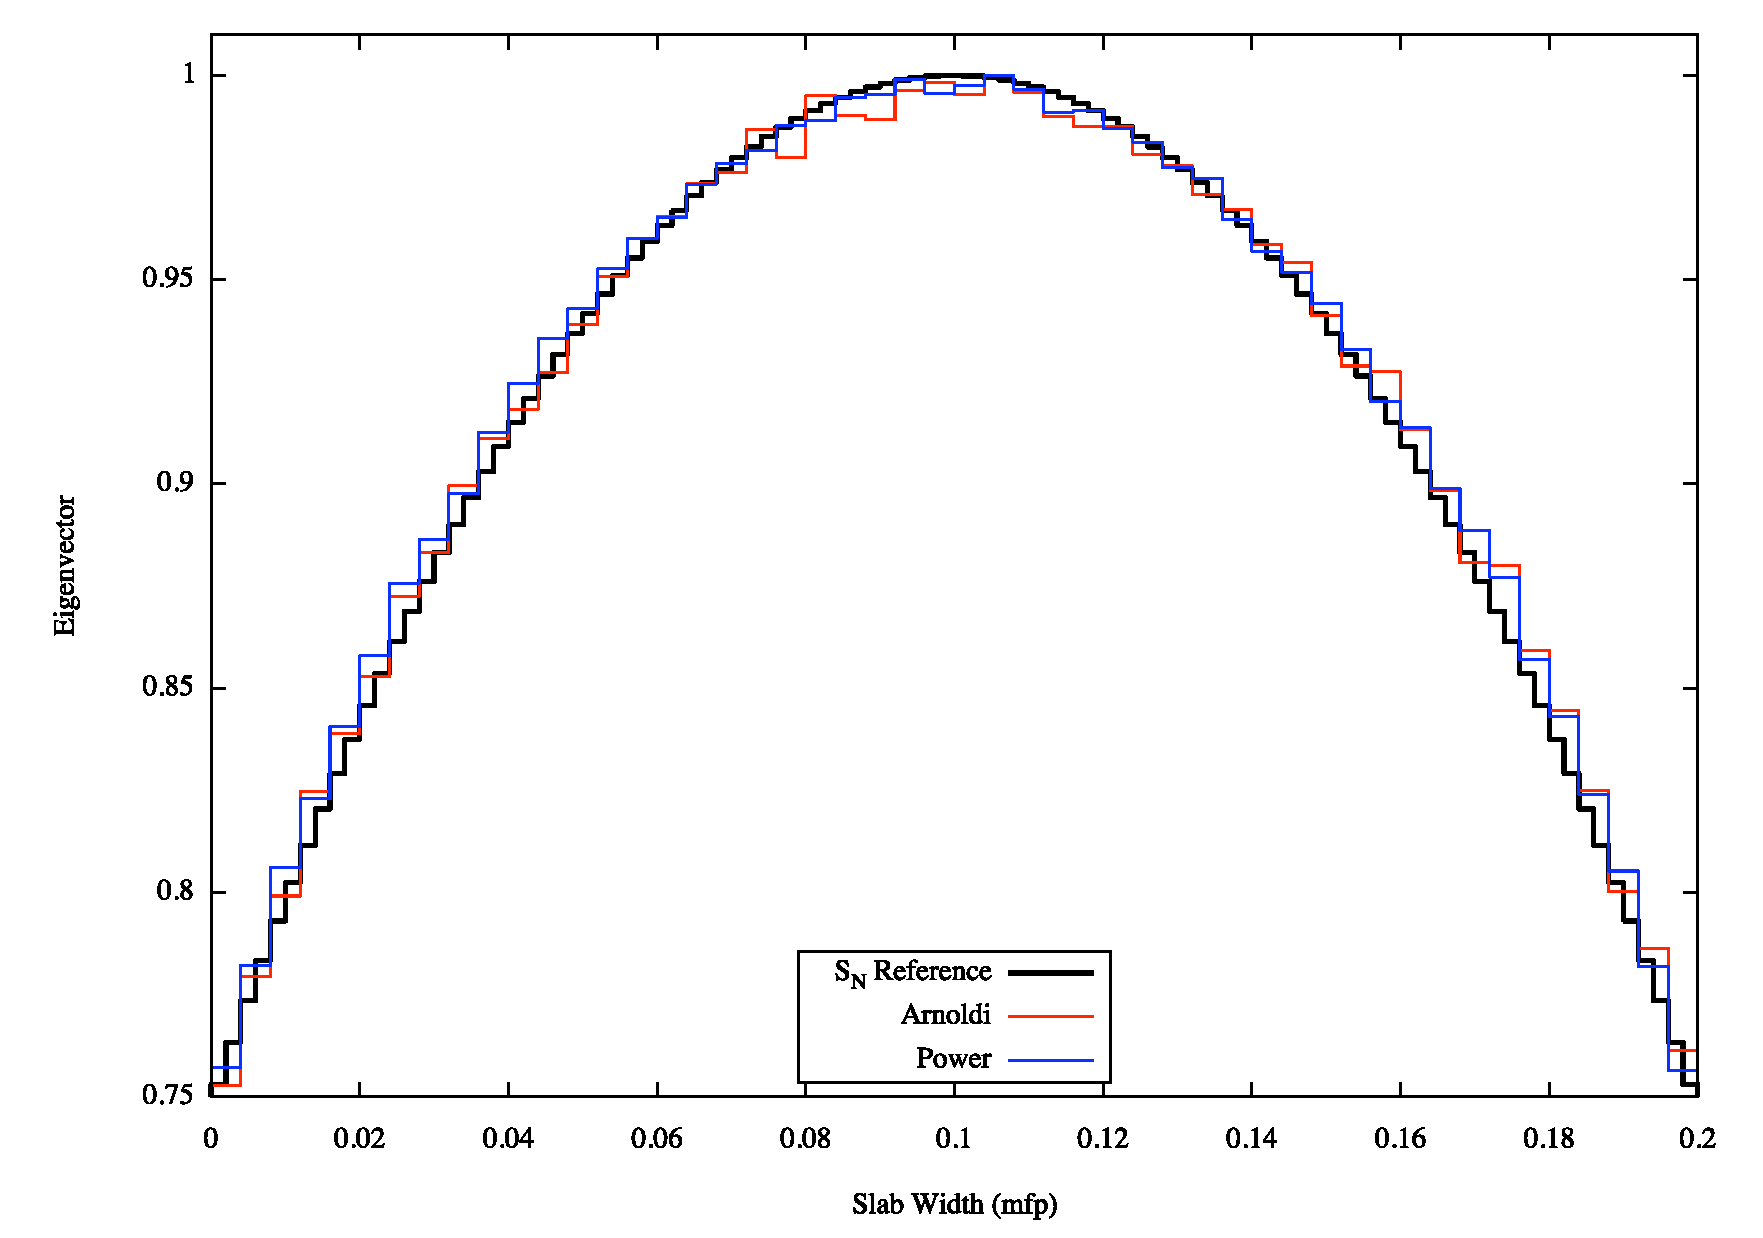
\includegraphics[width=\textwidth, keepaspectratio]{Arnoldi/Data/BasicFundamental-w02}
    % GNUPLOT: LaTeX picture with Postscript
\begingroup%
\makeatletter%
\newcommand{\GNUPLOTspecial}{%
  \@sanitize\catcode`\%=14\relax\special}%
\setlength{\unitlength}{0.0500bp}%
\begin{picture}(12960,8640)(0,0)%
  {\GNUPLOTspecial{"
%!PS-Adobe-2.0 EPSF-2.0
%%Title: BasicFundamental-w0.2.tex
%%Creator: gnuplot 4.3 patchlevel 0
%%CreationDate: Tue Jul 28 13:52:06 2009
%%DocumentFonts: 
%%BoundingBox: 0 0 648 432
%%EndComments
%%BeginProlog
/gnudict 256 dict def
gnudict begin
%
% The following true/false flags may be edited by hand if desired.
% The unit line width and grayscale image gamma correction may also be changed.
%
/Color true def
/Blacktext true def
/Solid true def
/Dashlength 1 def
/Landscape false def
/Level1 false def
/Rounded false def
/ClipToBoundingBox false def
/TransparentPatterns false def
/gnulinewidth 5.000 def
/userlinewidth gnulinewidth def
/Gamma 1.0 def
%
/vshift -66 def
/dl1 {
  10.0 Dashlength mul mul
  Rounded { currentlinewidth 0.75 mul sub dup 0 le { pop 0.01 } if } if
} def
/dl2 {
  10.0 Dashlength mul mul
  Rounded { currentlinewidth 0.75 mul add } if
} def
/hpt_ 31.5 def
/vpt_ 31.5 def
/hpt hpt_ def
/vpt vpt_ def
Level1 {} {
/SDict 10 dict def
systemdict /pdfmark known not {
  userdict /pdfmark systemdict /cleartomark get put
} if
SDict begin [
  /Title (BasicFundamental-w0.2.tex)
  /Subject (gnuplot plot)
  /Creator (gnuplot 4.3 patchlevel 0)
  /Author (Jeremy Conlin)
%  /Producer (gnuplot)
%  /Keywords ()
  /CreationDate (Tue Jul 28 13:52:06 2009)
  /DOCINFO pdfmark
end
} ifelse
/doclip {
  ClipToBoundingBox {
    newpath 0 0 moveto 648 0 lineto 648 432 lineto 0 432 lineto closepath
    clip
  } if
} def
%
% Gnuplot Prolog Version 4.2 (November 2007)
%
/M {moveto} bind def
/L {lineto} bind def
/R {rmoveto} bind def
/V {rlineto} bind def
/N {newpath moveto} bind def
/Z {closepath} bind def
/C {setrgbcolor} bind def
/f {rlineto fill} bind def
/Gshow {show} def   % May be redefined later in the file to support UTF-8
/vpt2 vpt 2 mul def
/hpt2 hpt 2 mul def
/Lshow {currentpoint stroke M 0 vshift R 
	Blacktext {gsave 0 setgray show grestore} {show} ifelse} def
/Rshow {currentpoint stroke M dup stringwidth pop neg vshift R
	Blacktext {gsave 0 setgray show grestore} {show} ifelse} def
/Cshow {currentpoint stroke M dup stringwidth pop -2 div vshift R 
	Blacktext {gsave 0 setgray show grestore} {show} ifelse} def
/UP {dup vpt_ mul /vpt exch def hpt_ mul /hpt exch def
  /hpt2 hpt 2 mul def /vpt2 vpt 2 mul def} def
/DL {Color {setrgbcolor Solid {pop []} if 0 setdash}
 {pop pop pop 0 setgray Solid {pop []} if 0 setdash} ifelse} def
/BL {stroke userlinewidth 2 mul setlinewidth
	Rounded {1 setlinejoin 1 setlinecap} if} def
/AL {stroke userlinewidth 2 div setlinewidth
	Rounded {1 setlinejoin 1 setlinecap} if} def
/UL {dup gnulinewidth mul /userlinewidth exch def
	dup 1 lt {pop 1} if 10 mul /udl exch def} def
/PL {stroke userlinewidth setlinewidth
	Rounded {1 setlinejoin 1 setlinecap} if} def
% Default Line colors
/LCw {1 1 1} def
/LCb {0 0 0} def
/LCa {0 0 0} def
/LC0 {1 0 0} def
/LC1 {0 1 0} def
/LC2 {0 0 1} def
/LC3 {1 0 1} def
/LC4 {0 1 1} def
/LC5 {1 1 0} def
/LC6 {0 0 0} def
/LC7 {1 0.3 0} def
/LC8 {0.5 0.5 0.5} def
% Default Line Types
/LTw {PL [] 1 setgray} def
/LTb {BL [] LCb DL} def
/LTa {AL [1 udl mul 2 udl mul] 0 setdash LCa setrgbcolor} def
/LT0 {PL [] LC0 DL} def
/LT1 {PL [4 dl1 2 dl2] LC1 DL} def
/LT2 {PL [2 dl1 3 dl2] LC2 DL} def
/LT3 {PL [1 dl1 1.5 dl2] LC3 DL} def
/LT4 {PL [6 dl1 2 dl2 1 dl1 2 dl2] LC4 DL} def
/LT5 {PL [3 dl1 3 dl2 1 dl1 3 dl2] LC5 DL} def
/LT6 {PL [2 dl1 2 dl2 2 dl1 6 dl2] LC6 DL} def
/LT7 {PL [1 dl1 2 dl2 6 dl1 2 dl2 1 dl1 2 dl2] LC7 DL} def
/LT8 {PL [2 dl1 2 dl2 2 dl1 2 dl2 2 dl1 2 dl2 2 dl1 4 dl2] LC8 DL} def
/Pnt {stroke [] 0 setdash gsave 1 setlinecap M 0 0 V stroke grestore} def
/Dia {stroke [] 0 setdash 2 copy vpt add M
  hpt neg vpt neg V hpt vpt neg V
  hpt vpt V hpt neg vpt V closepath stroke
  Pnt} def
/Pls {stroke [] 0 setdash vpt sub M 0 vpt2 V
  currentpoint stroke M
  hpt neg vpt neg R hpt2 0 V stroke
 } def
/Box {stroke [] 0 setdash 2 copy exch hpt sub exch vpt add M
  0 vpt2 neg V hpt2 0 V 0 vpt2 V
  hpt2 neg 0 V closepath stroke
  Pnt} def
/Crs {stroke [] 0 setdash exch hpt sub exch vpt add M
  hpt2 vpt2 neg V currentpoint stroke M
  hpt2 neg 0 R hpt2 vpt2 V stroke} def
/TriU {stroke [] 0 setdash 2 copy vpt 1.12 mul add M
  hpt neg vpt -1.62 mul V
  hpt 2 mul 0 V
  hpt neg vpt 1.62 mul V closepath stroke
  Pnt} def
/Star {2 copy Pls Crs} def
/BoxF {stroke [] 0 setdash exch hpt sub exch vpt add M
  0 vpt2 neg V hpt2 0 V 0 vpt2 V
  hpt2 neg 0 V closepath fill} def
/TriUF {stroke [] 0 setdash vpt 1.12 mul add M
  hpt neg vpt -1.62 mul V
  hpt 2 mul 0 V
  hpt neg vpt 1.62 mul V closepath fill} def
/TriD {stroke [] 0 setdash 2 copy vpt 1.12 mul sub M
  hpt neg vpt 1.62 mul V
  hpt 2 mul 0 V
  hpt neg vpt -1.62 mul V closepath stroke
  Pnt} def
/TriDF {stroke [] 0 setdash vpt 1.12 mul sub M
  hpt neg vpt 1.62 mul V
  hpt 2 mul 0 V
  hpt neg vpt -1.62 mul V closepath fill} def
/DiaF {stroke [] 0 setdash vpt add M
  hpt neg vpt neg V hpt vpt neg V
  hpt vpt V hpt neg vpt V closepath fill} def
/Pent {stroke [] 0 setdash 2 copy gsave
  translate 0 hpt M 4 {72 rotate 0 hpt L} repeat
  closepath stroke grestore Pnt} def
/PentF {stroke [] 0 setdash gsave
  translate 0 hpt M 4 {72 rotate 0 hpt L} repeat
  closepath fill grestore} def
/Circle {stroke [] 0 setdash 2 copy
  hpt 0 360 arc stroke Pnt} def
/CircleF {stroke [] 0 setdash hpt 0 360 arc fill} def
/C0 {BL [] 0 setdash 2 copy moveto vpt 90 450 arc} bind def
/C1 {BL [] 0 setdash 2 copy moveto
	2 copy vpt 0 90 arc closepath fill
	vpt 0 360 arc closepath} bind def
/C2 {BL [] 0 setdash 2 copy moveto
	2 copy vpt 90 180 arc closepath fill
	vpt 0 360 arc closepath} bind def
/C3 {BL [] 0 setdash 2 copy moveto
	2 copy vpt 0 180 arc closepath fill
	vpt 0 360 arc closepath} bind def
/C4 {BL [] 0 setdash 2 copy moveto
	2 copy vpt 180 270 arc closepath fill
	vpt 0 360 arc closepath} bind def
/C5 {BL [] 0 setdash 2 copy moveto
	2 copy vpt 0 90 arc
	2 copy moveto
	2 copy vpt 180 270 arc closepath fill
	vpt 0 360 arc} bind def
/C6 {BL [] 0 setdash 2 copy moveto
	2 copy vpt 90 270 arc closepath fill
	vpt 0 360 arc closepath} bind def
/C7 {BL [] 0 setdash 2 copy moveto
	2 copy vpt 0 270 arc closepath fill
	vpt 0 360 arc closepath} bind def
/C8 {BL [] 0 setdash 2 copy moveto
	2 copy vpt 270 360 arc closepath fill
	vpt 0 360 arc closepath} bind def
/C9 {BL [] 0 setdash 2 copy moveto
	2 copy vpt 270 450 arc closepath fill
	vpt 0 360 arc closepath} bind def
/C10 {BL [] 0 setdash 2 copy 2 copy moveto vpt 270 360 arc closepath fill
	2 copy moveto
	2 copy vpt 90 180 arc closepath fill
	vpt 0 360 arc closepath} bind def
/C11 {BL [] 0 setdash 2 copy moveto
	2 copy vpt 0 180 arc closepath fill
	2 copy moveto
	2 copy vpt 270 360 arc closepath fill
	vpt 0 360 arc closepath} bind def
/C12 {BL [] 0 setdash 2 copy moveto
	2 copy vpt 180 360 arc closepath fill
	vpt 0 360 arc closepath} bind def
/C13 {BL [] 0 setdash 2 copy moveto
	2 copy vpt 0 90 arc closepath fill
	2 copy moveto
	2 copy vpt 180 360 arc closepath fill
	vpt 0 360 arc closepath} bind def
/C14 {BL [] 0 setdash 2 copy moveto
	2 copy vpt 90 360 arc closepath fill
	vpt 0 360 arc} bind def
/C15 {BL [] 0 setdash 2 copy vpt 0 360 arc closepath fill
	vpt 0 360 arc closepath} bind def
/Rec {newpath 4 2 roll moveto 1 index 0 rlineto 0 exch rlineto
	neg 0 rlineto closepath} bind def
/Square {dup Rec} bind def
/Bsquare {vpt sub exch vpt sub exch vpt2 Square} bind def
/S0 {BL [] 0 setdash 2 copy moveto 0 vpt rlineto BL Bsquare} bind def
/S1 {BL [] 0 setdash 2 copy vpt Square fill Bsquare} bind def
/S2 {BL [] 0 setdash 2 copy exch vpt sub exch vpt Square fill Bsquare} bind def
/S3 {BL [] 0 setdash 2 copy exch vpt sub exch vpt2 vpt Rec fill Bsquare} bind def
/S4 {BL [] 0 setdash 2 copy exch vpt sub exch vpt sub vpt Square fill Bsquare} bind def
/S5 {BL [] 0 setdash 2 copy 2 copy vpt Square fill
	exch vpt sub exch vpt sub vpt Square fill Bsquare} bind def
/S6 {BL [] 0 setdash 2 copy exch vpt sub exch vpt sub vpt vpt2 Rec fill Bsquare} bind def
/S7 {BL [] 0 setdash 2 copy exch vpt sub exch vpt sub vpt vpt2 Rec fill
	2 copy vpt Square fill Bsquare} bind def
/S8 {BL [] 0 setdash 2 copy vpt sub vpt Square fill Bsquare} bind def
/S9 {BL [] 0 setdash 2 copy vpt sub vpt vpt2 Rec fill Bsquare} bind def
/S10 {BL [] 0 setdash 2 copy vpt sub vpt Square fill 2 copy exch vpt sub exch vpt Square fill
	Bsquare} bind def
/S11 {BL [] 0 setdash 2 copy vpt sub vpt Square fill 2 copy exch vpt sub exch vpt2 vpt Rec fill
	Bsquare} bind def
/S12 {BL [] 0 setdash 2 copy exch vpt sub exch vpt sub vpt2 vpt Rec fill Bsquare} bind def
/S13 {BL [] 0 setdash 2 copy exch vpt sub exch vpt sub vpt2 vpt Rec fill
	2 copy vpt Square fill Bsquare} bind def
/S14 {BL [] 0 setdash 2 copy exch vpt sub exch vpt sub vpt2 vpt Rec fill
	2 copy exch vpt sub exch vpt Square fill Bsquare} bind def
/S15 {BL [] 0 setdash 2 copy Bsquare fill Bsquare} bind def
/D0 {gsave translate 45 rotate 0 0 S0 stroke grestore} bind def
/D1 {gsave translate 45 rotate 0 0 S1 stroke grestore} bind def
/D2 {gsave translate 45 rotate 0 0 S2 stroke grestore} bind def
/D3 {gsave translate 45 rotate 0 0 S3 stroke grestore} bind def
/D4 {gsave translate 45 rotate 0 0 S4 stroke grestore} bind def
/D5 {gsave translate 45 rotate 0 0 S5 stroke grestore} bind def
/D6 {gsave translate 45 rotate 0 0 S6 stroke grestore} bind def
/D7 {gsave translate 45 rotate 0 0 S7 stroke grestore} bind def
/D8 {gsave translate 45 rotate 0 0 S8 stroke grestore} bind def
/D9 {gsave translate 45 rotate 0 0 S9 stroke grestore} bind def
/D10 {gsave translate 45 rotate 0 0 S10 stroke grestore} bind def
/D11 {gsave translate 45 rotate 0 0 S11 stroke grestore} bind def
/D12 {gsave translate 45 rotate 0 0 S12 stroke grestore} bind def
/D13 {gsave translate 45 rotate 0 0 S13 stroke grestore} bind def
/D14 {gsave translate 45 rotate 0 0 S14 stroke grestore} bind def
/D15 {gsave translate 45 rotate 0 0 S15 stroke grestore} bind def
/DiaE {stroke [] 0 setdash vpt add M
  hpt neg vpt neg V hpt vpt neg V
  hpt vpt V hpt neg vpt V closepath stroke} def
/BoxE {stroke [] 0 setdash exch hpt sub exch vpt add M
  0 vpt2 neg V hpt2 0 V 0 vpt2 V
  hpt2 neg 0 V closepath stroke} def
/TriUE {stroke [] 0 setdash vpt 1.12 mul add M
  hpt neg vpt -1.62 mul V
  hpt 2 mul 0 V
  hpt neg vpt 1.62 mul V closepath stroke} def
/TriDE {stroke [] 0 setdash vpt 1.12 mul sub M
  hpt neg vpt 1.62 mul V
  hpt 2 mul 0 V
  hpt neg vpt -1.62 mul V closepath stroke} def
/PentE {stroke [] 0 setdash gsave
  translate 0 hpt M 4 {72 rotate 0 hpt L} repeat
  closepath stroke grestore} def
/CircE {stroke [] 0 setdash 
  hpt 0 360 arc stroke} def
/Opaque {gsave closepath 1 setgray fill grestore 0 setgray closepath} def
/DiaW {stroke [] 0 setdash vpt add M
  hpt neg vpt neg V hpt vpt neg V
  hpt vpt V hpt neg vpt V Opaque stroke} def
/BoxW {stroke [] 0 setdash exch hpt sub exch vpt add M
  0 vpt2 neg V hpt2 0 V 0 vpt2 V
  hpt2 neg 0 V Opaque stroke} def
/TriUW {stroke [] 0 setdash vpt 1.12 mul add M
  hpt neg vpt -1.62 mul V
  hpt 2 mul 0 V
  hpt neg vpt 1.62 mul V Opaque stroke} def
/TriDW {stroke [] 0 setdash vpt 1.12 mul sub M
  hpt neg vpt 1.62 mul V
  hpt 2 mul 0 V
  hpt neg vpt -1.62 mul V Opaque stroke} def
/PentW {stroke [] 0 setdash gsave
  translate 0 hpt M 4 {72 rotate 0 hpt L} repeat
  Opaque stroke grestore} def
/CircW {stroke [] 0 setdash 
  hpt 0 360 arc Opaque stroke} def
/BoxFill {gsave Rec 1 setgray fill grestore} def
/Density {
  /Fillden exch def
  currentrgbcolor
  /ColB exch def /ColG exch def /ColR exch def
  /ColR ColR Fillden mul Fillden sub 1 add def
  /ColG ColG Fillden mul Fillden sub 1 add def
  /ColB ColB Fillden mul Fillden sub 1 add def
  ColR ColG ColB setrgbcolor} def
/BoxColFill {gsave Rec PolyFill} def
/PolyFill {gsave Density fill grestore grestore} def
/h {rlineto rlineto rlineto gsave closepath fill grestore} bind def
%
% PostScript Level 1 Pattern Fill routine for rectangles
% Usage: x y w h s a XX PatternFill
%	x,y = lower left corner of box to be filled
%	w,h = width and height of box
%	  a = angle in degrees between lines and x-axis
%	 XX = 0/1 for no/yes cross-hatch
%
/PatternFill {gsave /PFa [ 9 2 roll ] def
  PFa 0 get PFa 2 get 2 div add PFa 1 get PFa 3 get 2 div add translate
  PFa 2 get -2 div PFa 3 get -2 div PFa 2 get PFa 3 get Rec
  gsave 1 setgray fill grestore clip
  currentlinewidth 0.5 mul setlinewidth
  /PFs PFa 2 get dup mul PFa 3 get dup mul add sqrt def
  0 0 M PFa 5 get rotate PFs -2 div dup translate
  0 1 PFs PFa 4 get div 1 add floor cvi
	{PFa 4 get mul 0 M 0 PFs V} for
  0 PFa 6 get ne {
	0 1 PFs PFa 4 get div 1 add floor cvi
	{PFa 4 get mul 0 2 1 roll M PFs 0 V} for
 } if
  stroke grestore} def
%
/languagelevel where
 {pop languagelevel} {1} ifelse
 2 lt
	{/InterpretLevel1 true def}
	{/InterpretLevel1 Level1 def}
 ifelse
%
% PostScript level 2 pattern fill definitions
%
/Level2PatternFill {
/Tile8x8 {/PaintType 2 /PatternType 1 /TilingType 1 /BBox [0 0 8 8] /XStep 8 /YStep 8}
	bind def
/KeepColor {currentrgbcolor [/Pattern /DeviceRGB] setcolorspace} bind def
<< Tile8x8
 /PaintProc {0.5 setlinewidth pop 0 0 M 8 8 L 0 8 M 8 0 L stroke} 
>> matrix makepattern
/Pat1 exch def
<< Tile8x8
 /PaintProc {0.5 setlinewidth pop 0 0 M 8 8 L 0 8 M 8 0 L stroke
	0 4 M 4 8 L 8 4 L 4 0 L 0 4 L stroke}
>> matrix makepattern
/Pat2 exch def
<< Tile8x8
 /PaintProc {0.5 setlinewidth pop 0 0 M 0 8 L
	8 8 L 8 0 L 0 0 L fill}
>> matrix makepattern
/Pat3 exch def
<< Tile8x8
 /PaintProc {0.5 setlinewidth pop -4 8 M 8 -4 L
	0 12 M 12 0 L stroke}
>> matrix makepattern
/Pat4 exch def
<< Tile8x8
 /PaintProc {0.5 setlinewidth pop -4 0 M 8 12 L
	0 -4 M 12 8 L stroke}
>> matrix makepattern
/Pat5 exch def
<< Tile8x8
 /PaintProc {0.5 setlinewidth pop -2 8 M 4 -4 L
	0 12 M 8 -4 L 4 12 M 10 0 L stroke}
>> matrix makepattern
/Pat6 exch def
<< Tile8x8
 /PaintProc {0.5 setlinewidth pop -2 0 M 4 12 L
	0 -4 M 8 12 L 4 -4 M 10 8 L stroke}
>> matrix makepattern
/Pat7 exch def
<< Tile8x8
 /PaintProc {0.5 setlinewidth pop 8 -2 M -4 4 L
	12 0 M -4 8 L 12 4 M 0 10 L stroke}
>> matrix makepattern
/Pat8 exch def
<< Tile8x8
 /PaintProc {0.5 setlinewidth pop 0 -2 M 12 4 L
	-4 0 M 12 8 L -4 4 M 8 10 L stroke}
>> matrix makepattern
/Pat9 exch def
/Pattern1 {PatternBgnd KeepColor Pat1 setpattern} bind def
/Pattern2 {PatternBgnd KeepColor Pat2 setpattern} bind def
/Pattern3 {PatternBgnd KeepColor Pat3 setpattern} bind def
/Pattern4 {PatternBgnd KeepColor Landscape {Pat5} {Pat4} ifelse setpattern} bind def
/Pattern5 {PatternBgnd KeepColor Landscape {Pat4} {Pat5} ifelse setpattern} bind def
/Pattern6 {PatternBgnd KeepColor Landscape {Pat9} {Pat6} ifelse setpattern} bind def
/Pattern7 {PatternBgnd KeepColor Landscape {Pat8} {Pat7} ifelse setpattern} bind def
} def
%
%
%End of PostScript Level 2 code
%
/PatternBgnd {
  TransparentPatterns {} {gsave 1 setgray fill grestore} ifelse
} def
%
% Substitute for Level 2 pattern fill codes with
% grayscale if Level 2 support is not selected.
%
/Level1PatternFill {
/Pattern1 {0.250 Density} bind def
/Pattern2 {0.500 Density} bind def
/Pattern3 {0.750 Density} bind def
/Pattern4 {0.125 Density} bind def
/Pattern5 {0.375 Density} bind def
/Pattern6 {0.625 Density} bind def
/Pattern7 {0.875 Density} bind def
} def
%
% Now test for support of Level 2 code
%
Level1 {Level1PatternFill} {Level2PatternFill} ifelse
%
/Symbol-Oblique /Symbol findfont [1 0 .167 1 0 0] makefont
dup length dict begin {1 index /FID eq {pop pop} {def} ifelse} forall
currentdict end definefont pop
end
%%EndProlog
gnudict begin
gsave
doclip
0 0 translate
0.050 0.050 scale
0 setgray
newpath
1.000 UL
LTb
1220 640 M
63 0 V
11276 0 R
-63 0 V
1220 2132 M
63 0 V
11276 0 R
-63 0 V
1220 3624 M
63 0 V
11276 0 R
-63 0 V
1220 5116 M
63 0 V
11276 0 R
-63 0 V
1220 6608 M
63 0 V
11276 0 R
-63 0 V
1220 8101 M
63 0 V
11276 0 R
-63 0 V
1220 640 M
0 63 V
0 7696 R
0 -63 V
2354 640 M
0 63 V
0 7696 R
0 -63 V
3488 640 M
0 63 V
0 7696 R
0 -63 V
4622 640 M
0 63 V
0 7696 R
0 -63 V
5756 640 M
0 63 V
0 7696 R
0 -63 V
6890 640 M
0 63 V
0 7696 R
0 -63 V
8023 640 M
0 63 V
0 7696 R
0 -63 V
9157 640 M
0 63 V
0 7696 R
0 -63 V
10291 640 M
0 63 V
0 7696 R
0 -63 V
11425 640 M
0 63 V
0 7696 R
0 -63 V
12559 640 M
0 63 V
0 7696 R
0 -63 V
stroke
1220 8399 N
0 -7759 V
11339 0 V
0 7759 V
-11339 0 V
Z stroke
LCb setrgbcolor
LTb
LCb setrgbcolor
LTb
LCb setrgbcolor
LTb
LCb setrgbcolor
LTb
1.000 UP
1.000 UL
LTb
1.000 UL
LTb
5718 703 N
0 800 V
2342 0 V
0 -800 V
-2342 0 V
Z stroke
5718 1503 M
2342 0 V
stroke
2.000 UL
LTb
LCb setrgbcolor
LTb
7398 1303 M
543 0 V
1220 640 M
0 90 V
113 0 V
0 310 V
114 0 V
0 302 V
113 0 V
0 296 V
114 0 V
0 287 V
113 0 V
0 280 V
113 0 V
0 272 V
114 0 V
0 266 V
113 0 V
0 258 V
114 0 V
0 251 V
113 0 V
0 244 V
113 0 V
0 238 V
114 0 V
0 230 V
113 0 V
0 224 V
113 0 V
0 217 V
114 0 V
0 209 V
113 0 V
0 205 V
114 0 V
0 196 V
113 0 V
0 191 V
113 0 V
0 185 V
114 0 V
0 177 V
113 0 V
0 172 V
114 0 V
0 165 V
113 0 V
0 159 V
113 0 V
0 153 V
114 0 V
0 146 V
113 0 V
0 141 V
114 0 V
0 134 V
113 0 V
0 129 V
113 0 V
0 121 V
114 0 V
0 117 V
113 0 V
0 111 V
113 0 V
0 104 V
114 0 V
0 98 V
113 0 V
0 93 V
114 0 V
0 87 V
113 0 V
0 80 V
113 0 V
0 76 V
114 0 V
0 69 V
113 0 V
0 62 V
114 0 V
0 58 V
113 0 V
0 52 V
113 0 V
0 46 V
114 0 V
0 39 V
113 0 V
0 35 V
114 0 V
0 29 V
113 0 V
0 23 V
113 0 V
0 17 V
114 0 V
0 11 V
113 0 V
0 6 V
170 0 V
0 -6 V
170 0 V
stroke 7116 8095 M
0 -11 V
114 0 V
0 -17 V
113 0 V
0 -23 V
113 0 V
0 -29 V
114 0 V
0 -35 V
113 0 V
0 -39 V
114 0 V
0 -46 V
113 0 V
0 -52 V
113 0 V
0 -58 V
114 0 V
0 -62 V
113 0 V
0 -69 V
114 0 V
0 -76 V
113 0 V
0 -80 V
113 0 V
0 -87 V
114 0 V
0 -93 V
113 0 V
0 -98 V
114 0 V
0 -104 V
113 0 V
0 -111 V
113 0 V
0 -117 V
114 0 V
0 -121 V
113 0 V
0 -129 V
113 0 V
0 -134 V
114 0 V
0 -141 V
113 0 V
0 -146 V
114 0 V
0 -153 V
113 0 V
0 -159 V
113 0 V
0 -165 V
114 0 V
0 -172 V
113 0 V
0 -177 V
114 0 V
0 -185 V
113 0 V
0 -191 V
113 0 V
0 -196 V
114 0 V
0 -205 V
113 0 V
0 -209 V
114 0 V
0 -217 V
113 0 V
0 -224 V
113 0 V
0 -230 V
114 0 V
0 -238 V
113 0 V
0 -244 V
113 0 V
0 -251 V
114 0 V
0 -258 V
113 0 V
0 -266 V
114 0 V
0 -272 V
113 0 V
0 -280 V
113 0 V
0 -287 V
114 0 V
0 -296 V
113 0 V
0 -302 V
114 0 V
0 -310 V
113 0 V
0 -90 V
stroke
1.000 UL
LT0
LCb setrgbcolor
LT0
7398 1103 M
543 0 V
1220 640 M
0 279 V
227 0 V
0 753 V
227 0 V
0 620 V
226 0 V
0 544 V
227 0 V
0 637 V
227 0 V
0 460 V
227 0 V
0 391 V
226 0 V
0 547 V
227 0 V
0 324 V
227 0 V
0 346 V
227 0 V
0 323 V
227 0 V
0 228 V
226 0 V
0 387 V
227 0 V
0 247 V
227 0 V
0 216 V
227 0 V
0 208 V
226 0 V
0 223 V
227 0 V
0 88 V
227 0 V
0 153 V
227 0 V
0 196 V
227 0 V
0 71 V
226 0 V
0 76 V
227 0 V
0 50 V
227 0 V
0 4 V
227 0 V
0 -19 V
226 0 V
0 109 V
227 0 V
0 -97 V
227 0 V
0 15 V
227 0 V
0 -33 V
227 0 V
0 -106 V
226 0 V
0 -85 V
227 0 V
0 -175 V
227 0 V
0 -74 V
227 0 V
0 -175 V
227 0 V
0 -186 V
226 0 V
0 -254 V
227 0 V
0 -268 V
227 0 V
0 -177 V
227 0 V
0 -284 V
226 0 V
0 -341 V
227 0 V
0 -341 V
227 0 V
0 -349 V
227 0 V
0 -394 V
227 0 V
0 -393 V
226 0 V
0 -411 V
227 0 V
0 -505 V
227 0 V
0 -586 V
227 0 V
0 -654 V
226 0 V
0 -550 V
227 0 V
0 -820 V
227 0 V
0 -218 V
stroke
LT2
LCb setrgbcolor
LT2
7398 903 M
543 0 V
1220 640 M
0 7461 V
227 0 V
0 298 V
10885 0 R
0 -161 V
227 0 V
0 -7598 V
stroke
LTb
1220 8399 N
0 -7759 V
11339 0 V
0 7759 V
-11339 0 V
Z stroke
1.000 UP
1.000 UL
LTb
stroke
grestore
end
showpage
  }}%
  \put(7278,903){\makebox(0,0)[r]{\strut{}Arnoldi}}%
  \put(7278,1103){\makebox(0,0)[r]{\strut{}Power}}%
  \put(7278,1303){\makebox(0,0)[r]{\strut{}$S_N$ Reference}}%
  \put(6889,140){\makebox(0,0){\strut{}Slab Width (mfp)}}%
  \put(280,4519){%
  \special{ps: gsave currentpoint currentpoint translate
270 rotate neg exch neg exch translate}%
  \makebox(0,0){\strut{}Eigenvector}%
  \special{ps: currentpoint grestore moveto}%
  }%
  \put(12559,440){\makebox(0,0){\strut{} 0.2}}%
  \put(11425,440){\makebox(0,0){\strut{} 0.18}}%
  \put(10291,440){\makebox(0,0){\strut{} 0.16}}%
  \put(9157,440){\makebox(0,0){\strut{} 0.14}}%
  \put(8023,440){\makebox(0,0){\strut{} 0.12}}%
  \put(6890,440){\makebox(0,0){\strut{} 0.1}}%
  \put(5756,440){\makebox(0,0){\strut{} 0.08}}%
  \put(4622,440){\makebox(0,0){\strut{} 0.06}}%
  \put(3488,440){\makebox(0,0){\strut{} 0.04}}%
  \put(2354,440){\makebox(0,0){\strut{} 0.02}}%
  \put(1220,440){\makebox(0,0){\strut{} 0}}%
  \put(1100,8101){\makebox(0,0)[r]{\strut{} 1}}%
  \put(1100,6608){\makebox(0,0)[r]{\strut{} 0.95}}%
  \put(1100,5116){\makebox(0,0)[r]{\strut{} 0.9}}%
  \put(1100,3624){\makebox(0,0)[r]{\strut{} 0.85}}%
  \put(1100,2132){\makebox(0,0)[r]{\strut{} 0.8}}%
  \put(1100,640){\makebox(0,0)[r]{\strut{} 0.75}}%
\end{picture}%
\endgroup
\endinput

    \caption{Fundamental eigenvector estimates from the power method and Arnoldi's method for the 0.2 mfp wide slab.  The heavy line shows the S$_\mathrm{N}$ solution.}
    \label{fig:BasicFundamentalW02}
\end{sidewaysfigure}
\end{comment}

\begin{figure}\centering
    \subfloat[Eigenvalue estimates]{\label{fig:BasicValuesW2}% GNUPLOT: LaTeX picture with Postscript
\begingroup%
\makeatletter%
\newcommand{\GNUPLOTspecial}{%
  \@sanitize\catcode`\%=14\relax\special}%
\setlength{\unitlength}{0.0500bp}%
\begin{picture}(8640,5760)(0,0)%
  {\GNUPLOTspecial{"
%!PS-Adobe-2.0 EPSF-2.0
%%Title: BasicValues-w2.tex
%%Creator: gnuplot 4.3 patchlevel 0
%%CreationDate: Tue Jul 28 13:52:07 2009
%%DocumentFonts: 
%%BoundingBox: 0 0 432 288
%%EndComments
%%BeginProlog
/gnudict 256 dict def
gnudict begin
%
% The following true/false flags may be edited by hand if desired.
% The unit line width and grayscale image gamma correction may also be changed.
%
/Color true def
/Blacktext true def
/Solid true def
/Dashlength 1 def
/Landscape false def
/Level1 false def
/Rounded false def
/ClipToBoundingBox false def
/TransparentPatterns false def
/gnulinewidth 5.000 def
/userlinewidth gnulinewidth def
/Gamma 1.0 def
%
/vshift -66 def
/dl1 {
  10.0 Dashlength mul mul
  Rounded { currentlinewidth 0.75 mul sub dup 0 le { pop 0.01 } if } if
} def
/dl2 {
  10.0 Dashlength mul mul
  Rounded { currentlinewidth 0.75 mul add } if
} def
/hpt_ 31.5 def
/vpt_ 31.5 def
/hpt hpt_ def
/vpt vpt_ def
Level1 {} {
/SDict 10 dict def
systemdict /pdfmark known not {
  userdict /pdfmark systemdict /cleartomark get put
} if
SDict begin [
  /Title (BasicValues-w2.tex)
  /Subject (gnuplot plot)
  /Creator (gnuplot 4.3 patchlevel 0)
  /Author (Jeremy Conlin)
%  /Producer (gnuplot)
%  /Keywords ()
  /CreationDate (Tue Jul 28 13:52:07 2009)
  /DOCINFO pdfmark
end
} ifelse
/doclip {
  ClipToBoundingBox {
    newpath 0 0 moveto 432 0 lineto 432 288 lineto 0 288 lineto closepath
    clip
  } if
} def
%
% Gnuplot Prolog Version 4.2 (November 2007)
%
/M {moveto} bind def
/L {lineto} bind def
/R {rmoveto} bind def
/V {rlineto} bind def
/N {newpath moveto} bind def
/Z {closepath} bind def
/C {setrgbcolor} bind def
/f {rlineto fill} bind def
/Gshow {show} def   % May be redefined later in the file to support UTF-8
/vpt2 vpt 2 mul def
/hpt2 hpt 2 mul def
/Lshow {currentpoint stroke M 0 vshift R 
	Blacktext {gsave 0 setgray show grestore} {show} ifelse} def
/Rshow {currentpoint stroke M dup stringwidth pop neg vshift R
	Blacktext {gsave 0 setgray show grestore} {show} ifelse} def
/Cshow {currentpoint stroke M dup stringwidth pop -2 div vshift R 
	Blacktext {gsave 0 setgray show grestore} {show} ifelse} def
/UP {dup vpt_ mul /vpt exch def hpt_ mul /hpt exch def
  /hpt2 hpt 2 mul def /vpt2 vpt 2 mul def} def
/DL {Color {setrgbcolor Solid {pop []} if 0 setdash}
 {pop pop pop 0 setgray Solid {pop []} if 0 setdash} ifelse} def
/BL {stroke userlinewidth 2 mul setlinewidth
	Rounded {1 setlinejoin 1 setlinecap} if} def
/AL {stroke userlinewidth 2 div setlinewidth
	Rounded {1 setlinejoin 1 setlinecap} if} def
/UL {dup gnulinewidth mul /userlinewidth exch def
	dup 1 lt {pop 1} if 10 mul /udl exch def} def
/PL {stroke userlinewidth setlinewidth
	Rounded {1 setlinejoin 1 setlinecap} if} def
% Default Line colors
/LCw {1 1 1} def
/LCb {0 0 0} def
/LCa {0 0 0} def
/LC0 {1 0 0} def
/LC1 {0 1 0} def
/LC2 {0 0 1} def
/LC3 {1 0 1} def
/LC4 {0 1 1} def
/LC5 {1 1 0} def
/LC6 {0 0 0} def
/LC7 {1 0.3 0} def
/LC8 {0.5 0.5 0.5} def
% Default Line Types
/LTw {PL [] 1 setgray} def
/LTb {BL [] LCb DL} def
/LTa {AL [1 udl mul 2 udl mul] 0 setdash LCa setrgbcolor} def
/LT0 {PL [] LC0 DL} def
/LT1 {PL [4 dl1 2 dl2] LC1 DL} def
/LT2 {PL [2 dl1 3 dl2] LC2 DL} def
/LT3 {PL [1 dl1 1.5 dl2] LC3 DL} def
/LT4 {PL [6 dl1 2 dl2 1 dl1 2 dl2] LC4 DL} def
/LT5 {PL [3 dl1 3 dl2 1 dl1 3 dl2] LC5 DL} def
/LT6 {PL [2 dl1 2 dl2 2 dl1 6 dl2] LC6 DL} def
/LT7 {PL [1 dl1 2 dl2 6 dl1 2 dl2 1 dl1 2 dl2] LC7 DL} def
/LT8 {PL [2 dl1 2 dl2 2 dl1 2 dl2 2 dl1 2 dl2 2 dl1 4 dl2] LC8 DL} def
/Pnt {stroke [] 0 setdash gsave 1 setlinecap M 0 0 V stroke grestore} def
/Dia {stroke [] 0 setdash 2 copy vpt add M
  hpt neg vpt neg V hpt vpt neg V
  hpt vpt V hpt neg vpt V closepath stroke
  Pnt} def
/Pls {stroke [] 0 setdash vpt sub M 0 vpt2 V
  currentpoint stroke M
  hpt neg vpt neg R hpt2 0 V stroke
 } def
/Box {stroke [] 0 setdash 2 copy exch hpt sub exch vpt add M
  0 vpt2 neg V hpt2 0 V 0 vpt2 V
  hpt2 neg 0 V closepath stroke
  Pnt} def
/Crs {stroke [] 0 setdash exch hpt sub exch vpt add M
  hpt2 vpt2 neg V currentpoint stroke M
  hpt2 neg 0 R hpt2 vpt2 V stroke} def
/TriU {stroke [] 0 setdash 2 copy vpt 1.12 mul add M
  hpt neg vpt -1.62 mul V
  hpt 2 mul 0 V
  hpt neg vpt 1.62 mul V closepath stroke
  Pnt} def
/Star {2 copy Pls Crs} def
/BoxF {stroke [] 0 setdash exch hpt sub exch vpt add M
  0 vpt2 neg V hpt2 0 V 0 vpt2 V
  hpt2 neg 0 V closepath fill} def
/TriUF {stroke [] 0 setdash vpt 1.12 mul add M
  hpt neg vpt -1.62 mul V
  hpt 2 mul 0 V
  hpt neg vpt 1.62 mul V closepath fill} def
/TriD {stroke [] 0 setdash 2 copy vpt 1.12 mul sub M
  hpt neg vpt 1.62 mul V
  hpt 2 mul 0 V
  hpt neg vpt -1.62 mul V closepath stroke
  Pnt} def
/TriDF {stroke [] 0 setdash vpt 1.12 mul sub M
  hpt neg vpt 1.62 mul V
  hpt 2 mul 0 V
  hpt neg vpt -1.62 mul V closepath fill} def
/DiaF {stroke [] 0 setdash vpt add M
  hpt neg vpt neg V hpt vpt neg V
  hpt vpt V hpt neg vpt V closepath fill} def
/Pent {stroke [] 0 setdash 2 copy gsave
  translate 0 hpt M 4 {72 rotate 0 hpt L} repeat
  closepath stroke grestore Pnt} def
/PentF {stroke [] 0 setdash gsave
  translate 0 hpt M 4 {72 rotate 0 hpt L} repeat
  closepath fill grestore} def
/Circle {stroke [] 0 setdash 2 copy
  hpt 0 360 arc stroke Pnt} def
/CircleF {stroke [] 0 setdash hpt 0 360 arc fill} def
/C0 {BL [] 0 setdash 2 copy moveto vpt 90 450 arc} bind def
/C1 {BL [] 0 setdash 2 copy moveto
	2 copy vpt 0 90 arc closepath fill
	vpt 0 360 arc closepath} bind def
/C2 {BL [] 0 setdash 2 copy moveto
	2 copy vpt 90 180 arc closepath fill
	vpt 0 360 arc closepath} bind def
/C3 {BL [] 0 setdash 2 copy moveto
	2 copy vpt 0 180 arc closepath fill
	vpt 0 360 arc closepath} bind def
/C4 {BL [] 0 setdash 2 copy moveto
	2 copy vpt 180 270 arc closepath fill
	vpt 0 360 arc closepath} bind def
/C5 {BL [] 0 setdash 2 copy moveto
	2 copy vpt 0 90 arc
	2 copy moveto
	2 copy vpt 180 270 arc closepath fill
	vpt 0 360 arc} bind def
/C6 {BL [] 0 setdash 2 copy moveto
	2 copy vpt 90 270 arc closepath fill
	vpt 0 360 arc closepath} bind def
/C7 {BL [] 0 setdash 2 copy moveto
	2 copy vpt 0 270 arc closepath fill
	vpt 0 360 arc closepath} bind def
/C8 {BL [] 0 setdash 2 copy moveto
	2 copy vpt 270 360 arc closepath fill
	vpt 0 360 arc closepath} bind def
/C9 {BL [] 0 setdash 2 copy moveto
	2 copy vpt 270 450 arc closepath fill
	vpt 0 360 arc closepath} bind def
/C10 {BL [] 0 setdash 2 copy 2 copy moveto vpt 270 360 arc closepath fill
	2 copy moveto
	2 copy vpt 90 180 arc closepath fill
	vpt 0 360 arc closepath} bind def
/C11 {BL [] 0 setdash 2 copy moveto
	2 copy vpt 0 180 arc closepath fill
	2 copy moveto
	2 copy vpt 270 360 arc closepath fill
	vpt 0 360 arc closepath} bind def
/C12 {BL [] 0 setdash 2 copy moveto
	2 copy vpt 180 360 arc closepath fill
	vpt 0 360 arc closepath} bind def
/C13 {BL [] 0 setdash 2 copy moveto
	2 copy vpt 0 90 arc closepath fill
	2 copy moveto
	2 copy vpt 180 360 arc closepath fill
	vpt 0 360 arc closepath} bind def
/C14 {BL [] 0 setdash 2 copy moveto
	2 copy vpt 90 360 arc closepath fill
	vpt 0 360 arc} bind def
/C15 {BL [] 0 setdash 2 copy vpt 0 360 arc closepath fill
	vpt 0 360 arc closepath} bind def
/Rec {newpath 4 2 roll moveto 1 index 0 rlineto 0 exch rlineto
	neg 0 rlineto closepath} bind def
/Square {dup Rec} bind def
/Bsquare {vpt sub exch vpt sub exch vpt2 Square} bind def
/S0 {BL [] 0 setdash 2 copy moveto 0 vpt rlineto BL Bsquare} bind def
/S1 {BL [] 0 setdash 2 copy vpt Square fill Bsquare} bind def
/S2 {BL [] 0 setdash 2 copy exch vpt sub exch vpt Square fill Bsquare} bind def
/S3 {BL [] 0 setdash 2 copy exch vpt sub exch vpt2 vpt Rec fill Bsquare} bind def
/S4 {BL [] 0 setdash 2 copy exch vpt sub exch vpt sub vpt Square fill Bsquare} bind def
/S5 {BL [] 0 setdash 2 copy 2 copy vpt Square fill
	exch vpt sub exch vpt sub vpt Square fill Bsquare} bind def
/S6 {BL [] 0 setdash 2 copy exch vpt sub exch vpt sub vpt vpt2 Rec fill Bsquare} bind def
/S7 {BL [] 0 setdash 2 copy exch vpt sub exch vpt sub vpt vpt2 Rec fill
	2 copy vpt Square fill Bsquare} bind def
/S8 {BL [] 0 setdash 2 copy vpt sub vpt Square fill Bsquare} bind def
/S9 {BL [] 0 setdash 2 copy vpt sub vpt vpt2 Rec fill Bsquare} bind def
/S10 {BL [] 0 setdash 2 copy vpt sub vpt Square fill 2 copy exch vpt sub exch vpt Square fill
	Bsquare} bind def
/S11 {BL [] 0 setdash 2 copy vpt sub vpt Square fill 2 copy exch vpt sub exch vpt2 vpt Rec fill
	Bsquare} bind def
/S12 {BL [] 0 setdash 2 copy exch vpt sub exch vpt sub vpt2 vpt Rec fill Bsquare} bind def
/S13 {BL [] 0 setdash 2 copy exch vpt sub exch vpt sub vpt2 vpt Rec fill
	2 copy vpt Square fill Bsquare} bind def
/S14 {BL [] 0 setdash 2 copy exch vpt sub exch vpt sub vpt2 vpt Rec fill
	2 copy exch vpt sub exch vpt Square fill Bsquare} bind def
/S15 {BL [] 0 setdash 2 copy Bsquare fill Bsquare} bind def
/D0 {gsave translate 45 rotate 0 0 S0 stroke grestore} bind def
/D1 {gsave translate 45 rotate 0 0 S1 stroke grestore} bind def
/D2 {gsave translate 45 rotate 0 0 S2 stroke grestore} bind def
/D3 {gsave translate 45 rotate 0 0 S3 stroke grestore} bind def
/D4 {gsave translate 45 rotate 0 0 S4 stroke grestore} bind def
/D5 {gsave translate 45 rotate 0 0 S5 stroke grestore} bind def
/D6 {gsave translate 45 rotate 0 0 S6 stroke grestore} bind def
/D7 {gsave translate 45 rotate 0 0 S7 stroke grestore} bind def
/D8 {gsave translate 45 rotate 0 0 S8 stroke grestore} bind def
/D9 {gsave translate 45 rotate 0 0 S9 stroke grestore} bind def
/D10 {gsave translate 45 rotate 0 0 S10 stroke grestore} bind def
/D11 {gsave translate 45 rotate 0 0 S11 stroke grestore} bind def
/D12 {gsave translate 45 rotate 0 0 S12 stroke grestore} bind def
/D13 {gsave translate 45 rotate 0 0 S13 stroke grestore} bind def
/D14 {gsave translate 45 rotate 0 0 S14 stroke grestore} bind def
/D15 {gsave translate 45 rotate 0 0 S15 stroke grestore} bind def
/DiaE {stroke [] 0 setdash vpt add M
  hpt neg vpt neg V hpt vpt neg V
  hpt vpt V hpt neg vpt V closepath stroke} def
/BoxE {stroke [] 0 setdash exch hpt sub exch vpt add M
  0 vpt2 neg V hpt2 0 V 0 vpt2 V
  hpt2 neg 0 V closepath stroke} def
/TriUE {stroke [] 0 setdash vpt 1.12 mul add M
  hpt neg vpt -1.62 mul V
  hpt 2 mul 0 V
  hpt neg vpt 1.62 mul V closepath stroke} def
/TriDE {stroke [] 0 setdash vpt 1.12 mul sub M
  hpt neg vpt 1.62 mul V
  hpt 2 mul 0 V
  hpt neg vpt -1.62 mul V closepath stroke} def
/PentE {stroke [] 0 setdash gsave
  translate 0 hpt M 4 {72 rotate 0 hpt L} repeat
  closepath stroke grestore} def
/CircE {stroke [] 0 setdash 
  hpt 0 360 arc stroke} def
/Opaque {gsave closepath 1 setgray fill grestore 0 setgray closepath} def
/DiaW {stroke [] 0 setdash vpt add M
  hpt neg vpt neg V hpt vpt neg V
  hpt vpt V hpt neg vpt V Opaque stroke} def
/BoxW {stroke [] 0 setdash exch hpt sub exch vpt add M
  0 vpt2 neg V hpt2 0 V 0 vpt2 V
  hpt2 neg 0 V Opaque stroke} def
/TriUW {stroke [] 0 setdash vpt 1.12 mul add M
  hpt neg vpt -1.62 mul V
  hpt 2 mul 0 V
  hpt neg vpt 1.62 mul V Opaque stroke} def
/TriDW {stroke [] 0 setdash vpt 1.12 mul sub M
  hpt neg vpt 1.62 mul V
  hpt 2 mul 0 V
  hpt neg vpt -1.62 mul V Opaque stroke} def
/PentW {stroke [] 0 setdash gsave
  translate 0 hpt M 4 {72 rotate 0 hpt L} repeat
  Opaque stroke grestore} def
/CircW {stroke [] 0 setdash 
  hpt 0 360 arc Opaque stroke} def
/BoxFill {gsave Rec 1 setgray fill grestore} def
/Density {
  /Fillden exch def
  currentrgbcolor
  /ColB exch def /ColG exch def /ColR exch def
  /ColR ColR Fillden mul Fillden sub 1 add def
  /ColG ColG Fillden mul Fillden sub 1 add def
  /ColB ColB Fillden mul Fillden sub 1 add def
  ColR ColG ColB setrgbcolor} def
/BoxColFill {gsave Rec PolyFill} def
/PolyFill {gsave Density fill grestore grestore} def
/h {rlineto rlineto rlineto gsave closepath fill grestore} bind def
%
% PostScript Level 1 Pattern Fill routine for rectangles
% Usage: x y w h s a XX PatternFill
%	x,y = lower left corner of box to be filled
%	w,h = width and height of box
%	  a = angle in degrees between lines and x-axis
%	 XX = 0/1 for no/yes cross-hatch
%
/PatternFill {gsave /PFa [ 9 2 roll ] def
  PFa 0 get PFa 2 get 2 div add PFa 1 get PFa 3 get 2 div add translate
  PFa 2 get -2 div PFa 3 get -2 div PFa 2 get PFa 3 get Rec
  gsave 1 setgray fill grestore clip
  currentlinewidth 0.5 mul setlinewidth
  /PFs PFa 2 get dup mul PFa 3 get dup mul add sqrt def
  0 0 M PFa 5 get rotate PFs -2 div dup translate
  0 1 PFs PFa 4 get div 1 add floor cvi
	{PFa 4 get mul 0 M 0 PFs V} for
  0 PFa 6 get ne {
	0 1 PFs PFa 4 get div 1 add floor cvi
	{PFa 4 get mul 0 2 1 roll M PFs 0 V} for
 } if
  stroke grestore} def
%
/languagelevel where
 {pop languagelevel} {1} ifelse
 2 lt
	{/InterpretLevel1 true def}
	{/InterpretLevel1 Level1 def}
 ifelse
%
% PostScript level 2 pattern fill definitions
%
/Level2PatternFill {
/Tile8x8 {/PaintType 2 /PatternType 1 /TilingType 1 /BBox [0 0 8 8] /XStep 8 /YStep 8}
	bind def
/KeepColor {currentrgbcolor [/Pattern /DeviceRGB] setcolorspace} bind def
<< Tile8x8
 /PaintProc {0.5 setlinewidth pop 0 0 M 8 8 L 0 8 M 8 0 L stroke} 
>> matrix makepattern
/Pat1 exch def
<< Tile8x8
 /PaintProc {0.5 setlinewidth pop 0 0 M 8 8 L 0 8 M 8 0 L stroke
	0 4 M 4 8 L 8 4 L 4 0 L 0 4 L stroke}
>> matrix makepattern
/Pat2 exch def
<< Tile8x8
 /PaintProc {0.5 setlinewidth pop 0 0 M 0 8 L
	8 8 L 8 0 L 0 0 L fill}
>> matrix makepattern
/Pat3 exch def
<< Tile8x8
 /PaintProc {0.5 setlinewidth pop -4 8 M 8 -4 L
	0 12 M 12 0 L stroke}
>> matrix makepattern
/Pat4 exch def
<< Tile8x8
 /PaintProc {0.5 setlinewidth pop -4 0 M 8 12 L
	0 -4 M 12 8 L stroke}
>> matrix makepattern
/Pat5 exch def
<< Tile8x8
 /PaintProc {0.5 setlinewidth pop -2 8 M 4 -4 L
	0 12 M 8 -4 L 4 12 M 10 0 L stroke}
>> matrix makepattern
/Pat6 exch def
<< Tile8x8
 /PaintProc {0.5 setlinewidth pop -2 0 M 4 12 L
	0 -4 M 8 12 L 4 -4 M 10 8 L stroke}
>> matrix makepattern
/Pat7 exch def
<< Tile8x8
 /PaintProc {0.5 setlinewidth pop 8 -2 M -4 4 L
	12 0 M -4 8 L 12 4 M 0 10 L stroke}
>> matrix makepattern
/Pat8 exch def
<< Tile8x8
 /PaintProc {0.5 setlinewidth pop 0 -2 M 12 4 L
	-4 0 M 12 8 L -4 4 M 8 10 L stroke}
>> matrix makepattern
/Pat9 exch def
/Pattern1 {PatternBgnd KeepColor Pat1 setpattern} bind def
/Pattern2 {PatternBgnd KeepColor Pat2 setpattern} bind def
/Pattern3 {PatternBgnd KeepColor Pat3 setpattern} bind def
/Pattern4 {PatternBgnd KeepColor Landscape {Pat5} {Pat4} ifelse setpattern} bind def
/Pattern5 {PatternBgnd KeepColor Landscape {Pat4} {Pat5} ifelse setpattern} bind def
/Pattern6 {PatternBgnd KeepColor Landscape {Pat9} {Pat6} ifelse setpattern} bind def
/Pattern7 {PatternBgnd KeepColor Landscape {Pat8} {Pat7} ifelse setpattern} bind def
} def
%
%
%End of PostScript Level 2 code
%
/PatternBgnd {
  TransparentPatterns {} {gsave 1 setgray fill grestore} ifelse
} def
%
% Substitute for Level 2 pattern fill codes with
% grayscale if Level 2 support is not selected.
%
/Level1PatternFill {
/Pattern1 {0.250 Density} bind def
/Pattern2 {0.500 Density} bind def
/Pattern3 {0.750 Density} bind def
/Pattern4 {0.125 Density} bind def
/Pattern5 {0.375 Density} bind def
/Pattern6 {0.625 Density} bind def
/Pattern7 {0.875 Density} bind def
} def
%
% Now test for support of Level 2 code
%
Level1 {Level1PatternFill} {Level2PatternFill} ifelse
%
/Symbol-Oblique /Symbol findfont [1 0 .167 1 0 0] makefont
dup length dict begin {1 index /FID eq {pop pop} {def} ifelse} forall
currentdict end definefont pop
end
%%EndProlog
gnudict begin
gsave
doclip
0 0 translate
0.050 0.050 scale
0 setgray
newpath
1.000 UL
LTb
1100 640 M
63 0 V
7076 0 R
-63 0 V
1100 1182 M
63 0 V
7076 0 R
-63 0 V
1100 1724 M
63 0 V
7076 0 R
-63 0 V
1100 2266 M
63 0 V
7076 0 R
-63 0 V
1100 2808 M
63 0 V
7076 0 R
-63 0 V
1100 3351 M
63 0 V
7076 0 R
-63 0 V
1100 3893 M
63 0 V
7076 0 R
-63 0 V
1100 4435 M
63 0 V
7076 0 R
-63 0 V
1100 4977 M
63 0 V
7076 0 R
-63 0 V
1100 5519 M
63 0 V
7076 0 R
-63 0 V
1100 640 M
0 63 V
0 4816 R
0 -63 V
2120 640 M
0 63 V
0 4816 R
0 -63 V
3140 640 M
0 63 V
0 4816 R
0 -63 V
4160 640 M
0 63 V
0 4816 R
0 -63 V
5179 640 M
0 63 V
0 4816 R
0 -63 V
6199 640 M
0 63 V
0 4816 R
0 -63 V
7219 640 M
0 63 V
0 4816 R
0 -63 V
8239 640 M
0 63 V
0 4816 R
0 -63 V
stroke
1100 5519 N
0 -4879 V
7139 0 V
0 4879 V
-7139 0 V
Z stroke
LCb setrgbcolor
LTb
LCb setrgbcolor
LTb
LCb setrgbcolor
LTb
LCb setrgbcolor
LTb
1.000 UP
1.000 UL
LTb
1.000 UL
LTb
5776 2579 N
0 1000 V
2343 0 V
0 -1000 V
-2343 0 V
Z stroke
5776 3579 M
2343 0 V
1.000 UP
stroke
LT0
LCb setrgbcolor
LT0
7456 3379 M
543 0 V
-543 31 R
0 -62 V
543 62 R
0 -62 V
1105 2932 M
-31 0 R
62 0 V
-62 0 R
62 0 V
-26 1875 R
-31 0 R
62 0 V
-62 0 R
62 0 V
-26 327 R
-31 0 R
62 0 V
-62 0 R
62 0 V
-26 78 R
-31 0 R
62 0 V
-62 0 R
62 0 V
-26 7 R
-31 0 R
62 0 V
-62 0 R
62 0 V
-25 3 R
-31 0 R
62 0 V
-62 0 R
62 0 V
-26 46 R
-31 0 R
62 0 V
-62 0 R
62 0 V
-26 -40 R
-31 0 R
62 0 V
-62 0 R
62 0 V
-26 -8 R
-31 0 R
62 0 V
-62 0 R
62 0 V
-26 8 R
-31 0 R
62 0 V
-62 0 R
62 0 V
-26 -1 R
-31 0 R
62 0 V
-62 0 R
62 0 V
-26 -11 R
-31 0 R
62 0 V
-62 0 R
62 0 V
-26 14 R
-31 0 R
62 0 V
-62 0 R
62 0 V
-26 51 R
-31 0 R
62 0 V
-62 0 R
62 0 V
-26 -65 R
-31 0 R
62 0 V
-62 0 R
62 0 V
-25 16 R
-31 0 R
62 0 V
-62 0 R
62 0 V
-26 -25 R
-31 0 R
62 0 V
-62 0 R
62 0 V
-26 43 R
-31 0 R
62 0 V
-62 0 R
62 0 V
-26 -20 R
-31 0 R
62 0 V
-62 0 R
62 0 V
-26 4 R
-31 0 R
62 0 V
-62 0 R
62 0 V
stroke 1233 5234 M
-26 -6 R
-31 0 R
62 0 V
-62 0 R
62 0 V
-26 -40 R
-31 0 R
62 0 V
-62 0 R
62 0 V
-26 43 R
-31 0 R
62 0 V
-62 0 R
62 0 V
-26 40 R
-31 0 R
62 0 V
-62 0 R
62 0 V
-26 -54 R
-31 0 R
62 0 V
-62 0 R
62 0 V
-25 41 R
-31 0 R
62 0 V
-62 0 R
62 0 V
-26 -28 R
-31 0 R
62 0 V
-62 0 R
62 0 V
-26 -16 R
-31 0 R
62 0 V
-62 0 R
62 0 V
-26 -4 R
-31 0 R
62 0 V
-62 0 R
62 0 V
-26 -12 R
-31 0 R
62 0 V
-62 0 R
62 0 V
-26 26 R
-31 0 R
62 0 V
-62 0 R
62 0 V
-26 13 R
-31 0 R
62 0 V
-62 0 R
62 0 V
-26 -27 R
-31 0 R
62 0 V
-62 0 R
62 0 V
-26 34 R
-31 0 R
62 0 V
-62 0 R
62 0 V
-26 14 R
-31 0 R
62 0 V
-62 0 R
62 0 V
-25 -46 R
-31 0 R
62 0 V
-62 0 R
62 0 V
-26 63 R
-31 0 R
62 0 V
-62 0 R
62 0 V
-26 -67 R
-31 0 R
62 0 V
-62 0 R
62 0 V
-26 54 R
-31 0 R
62 0 V
-62 0 R
62 0 V
-26 7 R
-31 0 R
62 0 V
-62 0 R
62 0 V
-26 -10 R
-31 0 R
62 0 V
-62 0 R
62 0 V
stroke 1340 5259 M
-26 -27 R
-31 0 R
62 0 V
-62 0 R
62 0 V
-26 19 R
-31 0 R
62 0 V
-62 0 R
62 0 V
-26 -40 R
-31 0 R
62 0 V
-62 0 R
62 0 V
-26 35 R
-31 0 R
62 0 V
-62 0 R
62 0 V
-25 2 R
-31 0 R
62 0 V
-62 0 R
62 0 V
-26 -43 R
-31 0 R
62 0 V
-62 0 R
62 0 V
-26 89 R
-31 0 R
62 0 V
-62 0 R
62 0 V
-26 -68 R
-31 0 R
62 0 V
-62 0 R
62 0 V
-26 19 R
-31 0 R
62 0 V
-62 0 R
62 0 V
-26 8 R
-31 0 R
62 0 V
-62 0 R
62 0 V
-26 -18 R
-31 0 R
62 0 V
-62 0 R
62 0 V
-26 6 R
-31 0 R
62 0 V
-62 0 R
62 0 V
-26 -6 R
-31 0 R
62 0 V
-62 0 R
62 0 V
-26 16 R
-31 0 R
62 0 V
-62 0 R
62 0 V
-25 -41 R
-31 0 R
62 0 V
-62 0 R
62 0 V
-26 35 R
-31 0 R
62 0 V
-62 0 R
62 0 V
-26 -37 R
-31 0 R
62 0 V
-62 0 R
62 0 V
-26 54 R
-31 0 R
62 0 V
-62 0 R
62 0 V
-26 -23 R
-31 0 R
62 0 V
-62 0 R
62 0 V
-26 -3 R
-31 0 R
62 0 V
-62 0 R
62 0 V
-26 -30 R
-31 0 R
62 0 V
-62 0 R
62 0 V
stroke 1447 5206 M
-26 28 R
-31 0 R
62 0 V
-62 0 R
62 0 V
-26 -23 R
-31 0 R
62 0 V
-62 0 R
62 0 V
-26 50 R
-31 0 R
62 0 V
-62 0 R
62 0 V
-25 26 R
-31 0 R
62 0 V
-62 0 R
62 0 V
-26 -56 R
-31 0 R
62 0 V
-62 0 R
62 0 V
-26 21 R
-31 0 R
62 0 V
-62 0 R
62 0 V
-26 -24 R
-31 0 R
62 0 V
-62 0 R
62 0 V
-26 52 R
-31 0 R
62 0 V
-62 0 R
62 0 V
-26 -39 R
-31 0 R
62 0 V
-62 0 R
62 0 V
-26 -8 R
-31 0 R
62 0 V
-62 0 R
62 0 V
-26 14 R
-31 0 R
62 0 V
-62 0 R
62 0 V
-26 -16 R
-31 0 R
62 0 V
-62 0 R
62 0 V
-26 43 R
-31 0 R
62 0 V
-62 0 R
62 0 V
-25 -21 R
-31 0 R
62 0 V
-62 0 R
62 0 V
-26 -52 R
-31 0 R
62 0 V
-62 0 R
62 0 V
-26 57 R
-31 0 R
62 0 V
-62 0 R
62 0 V
-26 -30 R
-31 0 R
62 0 V
-62 0 R
62 0 V
-26 38 R
-31 0 R
62 0 V
-62 0 R
62 0 V
-26 24 R
-31 0 R
62 0 V
-62 0 R
62 0 V
-26 -62 R
-31 0 R
62 0 V
-62 0 R
62 0 V
-26 16 R
-31 0 R
62 0 V
-62 0 R
62 0 V
stroke 1554 5244 M
-26 2 R
-31 0 R
62 0 V
-62 0 R
62 0 V
-26 -29 R
-31 0 R
62 0 V
-62 0 R
62 0 V
-25 22 R
-31 0 R
62 0 V
-62 0 R
62 0 V
-26 6 R
-31 0 R
62 0 V
-62 0 R
62 0 V
-26 -21 R
-31 0 R
62 0 V
-62 0 R
62 0 V
-26 -16 R
-31 0 R
62 0 V
-62 0 R
62 0 V
-26 56 R
-31 0 R
62 0 V
-62 0 R
62 0 V
-26 -56 R
-31 0 R
62 0 V
-62 0 R
62 0 V
-26 32 R
-31 0 R
62 0 V
-62 0 R
62 0 V
-26 -3 R
-31 0 R
62 0 V
-62 0 R
62 0 V
-26 -12 R
-31 0 R
62 0 V
-62 0 R
62 0 V
-26 10 R
-31 0 R
62 0 V
-62 0 R
62 0 V
-25 -9 R
-31 0 R
62 0 V
-62 0 R
62 0 V
-26 2 R
-31 0 R
62 0 V
-62 0 R
62 0 V
-26 19 R
-31 0 R
62 0 V
-62 0 R
62 0 V
-26 3 R
-31 0 R
62 0 V
-62 0 R
62 0 V
-26 -5 R
-31 0 R
62 0 V
-62 0 R
62 0 V
-26 -59 R
-31 0 R
62 0 V
-62 0 R
62 0 V
-26 7 R
-31 0 R
62 0 V
-62 0 R
62 0 V
-26 39 R
-31 0 R
62 0 V
-62 0 R
62 0 V
-26 -42 R
-31 0 R
62 0 V
-62 0 R
62 0 V
stroke 1661 5190 M
-26 69 R
-31 0 R
62 0 V
-62 0 R
62 0 V
-25 3 R
-31 0 R
62 0 V
-62 0 R
62 0 V
-26 -35 R
-31 0 R
62 0 V
-62 0 R
62 0 V
-26 22 R
-31 0 R
62 0 V
-62 0 R
62 0 V
-26 -50 R
-31 0 R
62 0 V
-62 0 R
62 0 V
-26 8 R
-31 0 R
62 0 V
-62 0 R
62 0 V
-26 15 R
-31 0 R
62 0 V
-62 0 R
62 0 V
-26 40 R
-31 0 R
62 0 V
-62 0 R
62 0 V
-26 -13 R
-31 0 R
62 0 V
-62 0 R
62 0 V
-26 -15 R
-31 0 R
62 0 V
-62 0 R
62 0 V
-26 14 R
-31 0 R
62 0 V
-62 0 R
62 0 V
-25 -50 R
-31 0 R
62 0 V
-62 0 R
62 0 V
-26 50 R
-31 0 R
62 0 V
-62 0 R
62 0 V
-26 12 R
-31 0 R
62 0 V
-62 0 R
62 0 V
-26 -21 R
-31 0 R
62 0 V
-62 0 R
62 0 V
-26 -6 R
-31 0 R
62 0 V
-62 0 R
62 0 V
-26 15 R
-31 0 R
62 0 V
-62 0 R
62 0 V
-26 -26 R
-31 0 R
62 0 V
-62 0 R
62 0 V
-26 33 R
-31 0 R
62 0 V
-62 0 R
62 0 V
-26 4 R
-31 0 R
62 0 V
-62 0 R
62 0 V
-26 -13 R
-31 0 R
62 0 V
-62 0 R
62 0 V
stroke 1768 5246 M
-25 -17 R
-31 0 R
62 0 V
-62 0 R
62 0 V
-26 32 R
-31 0 R
62 0 V
-62 0 R
62 0 V
-26 -75 R
-31 0 R
62 0 V
-62 0 R
62 0 V
-26 25 R
-31 0 R
62 0 V
-62 0 R
62 0 V
-26 18 R
-31 0 R
62 0 V
-62 0 R
62 0 V
-26 19 R
-31 0 R
62 0 V
-62 0 R
62 0 V
-26 20 R
-31 0 R
62 0 V
-62 0 R
62 0 V
-26 -17 R
-31 0 R
62 0 V
-62 0 R
62 0 V
-26 -33 R
-31 0 R
62 0 V
-62 0 R
62 0 V
-26 22 R
-31 0 R
62 0 V
-62 0 R
62 0 V
-25 -17 R
-31 0 R
62 0 V
-62 0 R
62 0 V
-26 -13 R
-31 0 R
62 0 V
-62 0 R
62 0 V
-26 26 R
-31 0 R
62 0 V
-62 0 R
62 0 V
-26 -5 R
-31 0 R
62 0 V
-62 0 R
62 0 V
-26 7 R
-31 0 R
62 0 V
-62 0 R
62 0 V
-26 55 R
-31 0 R
62 0 V
-62 0 R
62 0 V
-26 -72 R
-31 0 R
62 0 V
-62 0 R
62 0 V
-26 25 R
-31 0 R
62 0 V
-62 0 R
62 0 V
-26 -12 R
-31 0 R
62 0 V
-62 0 R
62 0 V
-26 23 R
-31 0 R
62 0 V
-62 0 R
62 0 V
-26 -40 R
-31 0 R
62 0 V
-62 0 R
62 0 V
stroke 1875 5217 M
-25 30 R
-31 0 R
62 0 V
-62 0 R
62 0 V
-26 8 R
-31 0 R
62 0 V
-62 0 R
62 0 V
-26 10 R
-31 0 R
62 0 V
-62 0 R
62 0 V
-26 -4 R
-31 0 R
62 0 V
-62 0 R
62 0 V
-26 -19 R
-31 0 R
62 0 V
-62 0 R
62 0 V
-26 -23 R
-31 0 R
62 0 V
-62 0 R
62 0 V
-26 21 R
-31 0 R
62 0 V
-62 0 R
62 0 V
-26 -11 R
-31 0 R
62 0 V
-62 0 R
62 0 V
-26 28 R
-31 0 R
62 0 V
-62 0 R
62 0 V
-26 -19 R
-31 0 R
62 0 V
-62 0 R
62 0 V
-25 7 R
-31 0 R
62 0 V
-62 0 R
62 0 V
-26 -52 R
-31 0 R
62 0 V
-62 0 R
62 0 V
-26 53 R
-31 0 R
62 0 V
-62 0 R
62 0 V
-26 -17 R
-31 0 R
62 0 V
-62 0 R
62 0 V
-26 20 R
-31 0 R
62 0 V
-62 0 R
62 0 V
-26 55 R
-31 0 R
62 0 V
-62 0 R
62 0 V
-26 -38 R
-31 0 R
62 0 V
-62 0 R
62 0 V
-26 -31 R
-31 0 R
62 0 V
-62 0 R
62 0 V
-26 -22 R
-31 0 R
62 0 V
-62 0 R
62 0 V
-26 29 R
-31 0 R
62 0 V
-62 0 R
62 0 V
-25 2 R
-31 0 R
62 0 V
-62 0 R
62 0 V
stroke 1983 5244 M
-26 -18 R
-31 0 R
62 0 V
-62 0 R
62 0 V
-26 41 R
-31 0 R
62 0 V
-62 0 R
62 0 V
-26 -38 R
-31 0 R
62 0 V
-62 0 R
62 0 V
-26 14 R
-31 0 R
62 0 V
-62 0 R
62 0 V
-26 -2 R
-31 0 R
62 0 V
-62 0 R
62 0 V
-26 -20 R
-31 0 R
62 0 V
-62 0 R
62 0 V
-26 5 R
-31 0 R
62 0 V
-62 0 R
62 0 V
-26 23 R
-31 0 R
62 0 V
-62 0 R
62 0 V
-26 -18 R
-31 0 R
62 0 V
-62 0 R
62 0 V
-25 7 R
-31 0 R
62 0 V
-62 0 R
62 0 V
-26 -55 R
-31 0 R
62 0 V
-62 0 R
62 0 V
-26 74 R
-31 0 R
62 0 V
-62 0 R
62 0 V
-26 -28 R
-31 0 R
62 0 V
-62 0 R
62 0 V
-26 -9 R
-31 0 R
62 0 V
-62 0 R
62 0 V
-26 20 R
-31 0 R
62 0 V
-62 0 R
62 0 V
-26 -18 R
-31 0 R
62 0 V
-62 0 R
62 0 V
-26 20 R
-31 0 R
62 0 V
-62 0 R
62 0 V
-26 29 R
-31 0 R
62 0 V
-62 0 R
62 0 V
-26 -34 R
-31 0 R
62 0 V
-62 0 R
62 0 V
-25 -11 R
-31 0 R
62 0 V
-62 0 R
62 0 V
-26 53 R
-31 0 R
62 0 V
-62 0 R
62 0 V
stroke 2090 5279 M
-26 -1 R
-31 0 R
62 0 V
-62 0 R
62 0 V
-26 -10 R
-31 0 R
62 0 V
-62 0 R
62 0 V
-26 -48 R
-31 0 R
62 0 V
-62 0 R
62 0 V
-26 22 R
-31 0 R
62 0 V
-62 0 R
62 0 V
-26 -23 R
-31 0 R
62 0 V
-62 0 R
62 0 V
-26 34 R
-31 0 R
62 0 V
-62 0 R
62 0 V
-26 -40 R
-31 0 R
62 0 V
-62 0 R
62 0 V
-26 -7 R
-31 0 R
62 0 V
-62 0 R
62 0 V
-25 41 R
-31 0 R
62 0 V
-62 0 R
62 0 V
-26 -5 R
-31 0 R
62 0 V
-62 0 R
62 0 V
-26 -5 R
-31 0 R
62 0 V
-62 0 R
62 0 V
-26 29 R
-31 0 R
62 0 V
-62 0 R
62 0 V
-26 -41 R
-31 0 R
62 0 V
-62 0 R
62 0 V
-26 45 R
-31 0 R
62 0 V
-62 0 R
62 0 V
-26 -15 R
-31 0 R
62 0 V
-62 0 R
62 0 V
-26 17 R
-31 0 R
62 0 V
-62 0 R
62 0 V
-26 -66 R
-31 0 R
62 0 V
-62 0 R
62 0 V
-26 18 R
-31 0 R
62 0 V
-62 0 R
62 0 V
-25 18 R
-31 0 R
62 0 V
-62 0 R
62 0 V
-26 -12 R
-31 0 R
62 0 V
-62 0 R
62 0 V
-26 15 R
-31 0 R
62 0 V
-62 0 R
62 0 V
stroke 2197 5245 M
-26 7 R
-31 0 R
62 0 V
-62 0 R
62 0 V
-26 -1 R
-31 0 R
62 0 V
-62 0 R
62 0 V
-26 -13 R
-31 0 R
62 0 V
-62 0 R
62 0 V
-26 22 R
-31 0 R
62 0 V
-62 0 R
62 0 V
-26 -42 R
-31 0 R
62 0 V
-62 0 R
62 0 V
-26 53 R
-31 0 R
62 0 V
-62 0 R
62 0 V
-26 -45 R
-31 0 R
62 0 V
-62 0 R
62 0 V
-25 -15 R
-31 0 R
62 0 V
-62 0 R
62 0 V
-26 12 R
-31 0 R
62 0 V
-62 0 R
62 0 V
-26 -22 R
-31 0 R
62 0 V
-62 0 R
62 0 V
-26 38 R
-31 0 R
62 0 V
-62 0 R
62 0 V
-26 -24 R
-31 0 R
62 0 V
-62 0 R
62 0 V
-26 53 R
-31 0 R
62 0 V
-62 0 R
62 0 V
-26 -33 R
-31 0 R
62 0 V
-62 0 R
62 0 V
-26 31 R
-31 0 R
62 0 V
-62 0 R
62 0 V
-26 -46 R
-31 0 R
62 0 V
-62 0 R
62 0 V
-26 -19 R
-31 0 R
62 0 V
-62 0 R
62 0 V
-25 10 R
-31 0 R
62 0 V
-62 0 R
62 0 V
-26 38 R
-31 0 R
62 0 V
-62 0 R
62 0 V
-26 -53 R
-31 0 R
62 0 V
-62 0 R
62 0 V
-26 25 R
-31 0 R
62 0 V
-62 0 R
62 0 V
stroke 2304 5221 M
-26 10 R
-31 0 R
62 0 V
-62 0 R
62 0 V
-26 5 R
-31 0 R
62 0 V
-62 0 R
62 0 V
-26 19 R
-31 0 R
62 0 V
-62 0 R
62 0 V
-26 -43 R
-31 0 R
62 0 V
-62 0 R
62 0 V
-26 30 R
-31 0 R
62 0 V
-62 0 R
62 0 V
-26 24 R
-31 0 R
62 0 V
-62 0 R
62 0 V
-25 0 R
-31 0 R
62 0 V
-62 0 R
62 0 V
-26 -39 R
-31 0 R
62 0 V
-62 0 R
62 0 V
-26 -8 R
-31 0 R
62 0 V
-62 0 R
62 0 V
-26 7 R
-31 0 R
62 0 V
-62 0 R
62 0 V
-26 26 R
-31 0 R
62 0 V
-62 0 R
62 0 V
-26 -6 R
-31 0 R
62 0 V
-62 0 R
62 0 V
-26 -17 R
-31 0 R
62 0 V
-62 0 R
62 0 V
-26 -21 R
-31 0 R
62 0 V
-62 0 R
62 0 V
-26 58 R
-31 0 R
62 0 V
-62 0 R
62 0 V
-26 -11 R
-31 0 R
62 0 V
-62 0 R
62 0 V
-25 -52 R
-31 0 R
62 0 V
-62 0 R
62 0 V
-26 30 R
-31 0 R
62 0 V
-62 0 R
62 0 V
-26 0 R
-31 0 R
62 0 V
-62 0 R
62 0 V
-26 4 R
-31 0 R
62 0 V
-62 0 R
62 0 V
-26 -13 R
-31 0 R
62 0 V
-62 0 R
62 0 V
stroke 2411 5224 M
-26 3 R
0 16 V
-31 -16 R
62 0 V
-62 16 R
62 0 V
-26 -14 R
0 10 V
-31 -10 R
62 0 V
-62 10 R
62 0 V
-26 -17 R
0 13 V
-31 -13 R
62 0 V
-62 13 R
62 0 V
-26 -10 R
0 11 V
-31 -11 R
62 0 V
-62 11 R
62 0 V
-26 -12 R
0 10 V
-31 -10 R
62 0 V
-62 10 R
62 0 V
-25 -15 R
0 12 V
-31 -12 R
62 0 V
-62 12 R
62 0 V
-26 -7 R
0 18 V
-31 -18 R
62 0 V
-62 18 R
62 0 V
-26 -13 R
0 18 V
-31 -18 R
62 0 V
-62 18 R
62 0 V
-26 -17 R
0 16 V
-31 -16 R
62 0 V
-62 16 R
62 0 V
-26 -15 R
0 15 V
-31 -15 R
62 0 V
-62 15 R
62 0 V
-26 -15 R
0 14 V
-31 -14 R
62 0 V
-62 14 R
62 0 V
-26 -13 R
0 13 V
-31 -13 R
62 0 V
-62 13 R
62 0 V
-26 -12 R
0 12 V
-31 -12 R
62 0 V
-62 12 R
62 0 V
-26 -13 R
0 11 V
-31 -11 R
62 0 V
-62 11 R
62 0 V
-26 -12 R
0 11 V
-31 -11 R
62 0 V
-62 11 R
62 0 V
-25 -10 R
0 10 V
-31 -10 R
62 0 V
-62 10 R
62 0 V
-26 -10 R
0 10 V
-31 -10 R
62 0 V
-62 10 R
62 0 V
-26 -11 R
0 10 V
stroke 2472 5241 M
-31 -10 R
62 0 V
-62 10 R
62 0 V
-26 -11 R
0 9 V
-31 -9 R
62 0 V
-62 9 R
62 0 V
-26 -12 R
0 10 V
-31 -10 R
62 0 V
-62 10 R
62 0 V
-26 -10 R
0 10 V
-31 -10 R
62 0 V
-62 10 R
62 0 V
-26 -10 R
0 9 V
-31 -9 R
62 0 V
-62 9 R
62 0 V
-26 -10 R
0 9 V
-31 -9 R
62 0 V
-62 9 R
62 0 V
-26 -9 R
0 9 V
-31 -9 R
62 0 V
-62 9 R
62 0 V
-26 -9 R
0 9 V
-31 -9 R
62 0 V
-62 9 R
62 0 V
-25 -9 R
0 8 V
-31 -8 R
62 0 V
-62 8 R
62 0 V
-26 -7 R
0 8 V
-31 -8 R
62 0 V
-62 8 R
62 0 V
-26 -9 R
0 8 V
-31 -8 R
62 0 V
-62 8 R
62 0 V
-26 -7 R
0 9 V
-31 -9 R
62 0 V
-62 9 R
62 0 V
-26 -9 R
0 8 V
-31 -8 R
62 0 V
-62 8 R
62 0 V
-26 -9 R
0 8 V
-31 -8 R
62 0 V
-62 8 R
62 0 V
-26 -8 R
0 8 V
-31 -8 R
62 0 V
-62 8 R
62 0 V
-26 -8 R
0 8 V
-31 -8 R
62 0 V
-62 8 R
62 0 V
-26 -7 R
0 8 V
-31 -8 R
62 0 V
-62 8 R
62 0 V
-26 -7 R
0 8 V
-31 -8 R
62 0 V
stroke 2589 5228 M
-62 8 R
62 0 V
-26 -8 R
0 7 V
-31 -7 R
62 0 V
-62 7 R
62 0 V
-25 -6 R
0 7 V
-31 -7 R
62 0 V
-62 7 R
62 0 V
-26 -8 R
0 7 V
-31 -7 R
62 0 V
-62 7 R
62 0 V
-26 -7 R
0 7 V
-31 -7 R
62 0 V
-62 7 R
62 0 V
-26 -6 R
0 7 V
-31 -7 R
62 0 V
-62 7 R
62 0 V
-26 -8 R
0 7 V
-31 -7 R
62 0 V
-62 7 R
62 0 V
-26 -7 R
0 7 V
-31 -7 R
62 0 V
-62 7 R
62 0 V
-26 -6 R
0 6 V
-31 -6 R
62 0 V
-62 6 R
62 0 V
-26 -6 R
0 6 V
-31 -6 R
62 0 V
-62 6 R
62 0 V
-26 -6 R
0 6 V
-31 -6 R
62 0 V
-62 6 R
62 0 V
-26 -6 R
0 6 V
-31 -6 R
62 0 V
-62 6 R
62 0 V
-25 -6 R
0 6 V
-31 -6 R
62 0 V
-62 6 R
62 0 V
-26 -6 R
0 6 V
-31 -6 R
62 0 V
-62 6 R
62 0 V
-26 -6 R
0 6 V
-31 -6 R
62 0 V
-62 6 R
62 0 V
-26 -6 R
0 6 V
-31 -6 R
62 0 V
-62 6 R
62 0 V
-26 -6 R
0 6 V
-31 -6 R
62 0 V
-62 6 R
62 0 V
-26 -6 R
0 6 V
-31 -6 R
62 0 V
-62 6 R
62 0 V
stroke 2676 5235 M
-26 -5 R
0 5 V
-31 -5 R
62 0 V
-62 5 R
62 0 V
-26 -5 R
0 6 V
-31 -6 R
62 0 V
-62 6 R
62 0 V
-26 -5 R
0 5 V
-31 -5 R
62 0 V
-62 5 R
62 0 V
-26 -5 R
0 6 V
-31 -6 R
62 0 V
-62 6 R
62 0 V
-25 -6 R
0 6 V
-31 -6 R
62 0 V
-62 6 R
62 0 V
-26 -6 R
0 6 V
-31 -6 R
62 0 V
-62 6 R
62 0 V
-26 -5 R
0 5 V
-31 -5 R
62 0 V
-62 5 R
62 0 V
-26 -5 R
0 6 V
-31 -6 R
62 0 V
-62 6 R
62 0 V
-26 -5 R
0 5 V
-31 -5 R
62 0 V
-62 5 R
62 0 V
-26 -5 R
0 6 V
-31 -6 R
62 0 V
-62 6 R
62 0 V
-26 -5 R
0 5 V
-31 -5 R
62 0 V
-62 5 R
62 0 V
-26 -6 R
0 6 V
-31 -6 R
62 0 V
-62 6 R
62 0 V
-26 -6 R
0 6 V
-31 -6 R
62 0 V
-62 6 R
62 0 V
-26 -6 R
0 6 V
-31 -6 R
62 0 V
-62 6 R
62 0 V
-25 -5 R
0 5 V
-31 -5 R
62 0 V
-62 5 R
62 0 V
-26 -6 R
0 5 V
-31 -5 R
62 0 V
-62 5 R
62 0 V
-26 -5 R
0 5 V
-31 -5 R
62 0 V
-62 5 R
62 0 V
-26 -4 R
0 5 V
stroke 2737 5239 M
-31 -5 R
62 0 V
-62 5 R
62 0 V
-26 -5 R
0 5 V
-31 -5 R
62 0 V
-62 5 R
62 0 V
-26 -5 R
0 5 V
-31 -5 R
62 0 V
-62 5 R
62 0 V
-26 -5 R
0 5 V
-31 -5 R
62 0 V
-62 5 R
62 0 V
-26 -5 R
0 5 V
-31 -5 R
62 0 V
-62 5 R
62 0 V
-26 -6 R
0 5 V
-31 -5 R
62 0 V
-62 5 R
62 0 V
-26 -4 R
0 5 V
-31 -5 R
62 0 V
-62 5 R
62 0 V
-25 -5 R
0 5 V
-31 -5 R
62 0 V
-62 5 R
62 0 V
-26 -5 R
0 4 V
-31 -4 R
62 0 V
-62 4 R
62 0 V
-26 -4 R
0 4 V
-31 -4 R
62 0 V
-62 4 R
62 0 V
-26 -5 R
0 5 V
-31 -5 R
62 0 V
-62 5 R
62 0 V
-26 -4 R
0 4 V
-31 -4 R
62 0 V
-62 4 R
62 0 V
-26 -4 R
0 4 V
-31 -4 R
62 0 V
-62 4 R
62 0 V
-26 -4 R
0 4 V
-31 -4 R
62 0 V
-62 4 R
62 0 V
-26 -5 R
0 5 V
-31 -5 R
62 0 V
-62 5 R
62 0 V
-26 -4 R
0 5 V
-31 -5 R
62 0 V
-62 5 R
62 0 V
-26 -5 R
0 4 V
-31 -4 R
62 0 V
-62 4 R
62 0 V
-25 -5 R
0 5 V
-31 -5 R
62 0 V
stroke 2855 5233 M
-62 5 R
62 0 V
-26 -5 R
0 5 V
-31 -5 R
62 0 V
-62 5 R
62 0 V
-26 -4 R
0 4 V
-31 -4 R
62 0 V
-62 4 R
62 0 V
-26 -5 R
0 5 V
-31 -5 R
62 0 V
-62 5 R
62 0 V
-26 -5 R
0 5 V
-31 -5 R
62 0 V
-62 5 R
62 0 V
-26 -5 R
0 5 V
-31 -5 R
62 0 V
-62 5 R
62 0 V
-26 -5 R
0 4 V
-31 -4 R
62 0 V
-62 4 R
62 0 V
-26 -5 R
0 5 V
-31 -5 R
62 0 V
-62 5 R
62 0 V
-26 -5 R
0 5 V
-31 -5 R
62 0 V
-62 5 R
62 0 V
-26 -5 R
0 5 V
-31 -5 R
62 0 V
-62 5 R
62 0 V
-25 -5 R
0 5 V
-31 -5 R
62 0 V
-62 5 R
62 0 V
-26 -5 R
0 5 V
-31 -5 R
62 0 V
-62 5 R
62 0 V
-26 -5 R
0 5 V
-31 -5 R
62 0 V
-62 5 R
62 0 V
-26 -5 R
0 4 V
-31 -4 R
62 0 V
-62 4 R
62 0 V
-26 -4 R
0 4 V
-31 -4 R
62 0 V
-62 4 R
62 0 V
-26 -4 R
0 4 V
-31 -4 R
62 0 V
-62 4 R
62 0 V
-26 -4 R
0 5 V
-31 -5 R
62 0 V
-62 5 R
62 0 V
-26 -5 R
0 5 V
-31 -5 R
62 0 V
-62 5 R
62 0 V
stroke 2941 5237 M
-26 -5 R
0 4 V
-31 -4 R
62 0 V
-62 4 R
62 0 V
-26 -4 R
0 5 V
-31 -5 R
62 0 V
-62 5 R
62 0 V
-25 -5 R
0 5 V
-31 -5 R
62 0 V
-62 5 R
62 0 V
-26 -5 R
0 5 V
-31 -5 R
62 0 V
-62 5 R
62 0 V
-26 -5 R
0 5 V
-31 -5 R
62 0 V
-62 5 R
62 0 V
-26 -5 R
0 4 V
-31 -4 R
62 0 V
-62 4 R
62 0 V
-26 -4 R
0 4 V
-31 -4 R
62 0 V
-62 4 R
62 0 V
-26 -4 R
0 4 V
-31 -4 R
62 0 V
-62 4 R
62 0 V
-26 -4 R
0 4 V
-31 -4 R
62 0 V
-62 4 R
62 0 V
-26 -4 R
0 4 V
-31 -4 R
62 0 V
-62 4 R
62 0 V
-26 -4 R
0 4 V
-31 -4 R
62 0 V
-62 4 R
62 0 V
-26 -4 R
0 4 V
-31 -4 R
62 0 V
-62 4 R
62 0 V
-25 -4 R
0 5 V
-31 -5 R
62 0 V
-62 5 R
62 0 V
-26 -4 R
0 4 V
-31 -4 R
62 0 V
-62 4 R
62 0 V
-26 -4 R
0 4 V
-31 -4 R
62 0 V
-62 4 R
62 0 V
-26 -4 R
0 4 V
-31 -4 R
62 0 V
-62 4 R
62 0 V
-26 -4 R
0 4 V
-31 -4 R
62 0 V
-62 4 R
62 0 V
-26 -4 R
0 4 V
stroke 3002 5237 M
-31 -4 R
62 0 V
-62 4 R
62 0 V
-26 -4 R
0 4 V
-31 -4 R
62 0 V
-62 4 R
62 0 V
-26 -4 R
0 4 V
-31 -4 R
62 0 V
-62 4 R
62 0 V
-26 -3 R
0 4 V
-31 -4 R
62 0 V
-62 4 R
62 0 V
-26 -5 R
0 4 V
-31 -4 R
62 0 V
-62 4 R
62 0 V
-25 -4 R
0 4 V
-31 -4 R
62 0 V
-62 4 R
62 0 V
-26 -4 R
0 4 V
-31 -4 R
62 0 V
-62 4 R
62 0 V
-26 -4 R
0 5 V
-31 -5 R
62 0 V
-62 5 R
62 0 V
-26 -5 R
0 4 V
-31 -4 R
62 0 V
-62 4 R
62 0 V
-26 -4 R
0 4 V
-31 -4 R
62 0 V
-62 4 R
62 0 V
-26 -4 R
0 4 V
-31 -4 R
62 0 V
-62 4 R
62 0 V
-26 -4 R
0 4 V
-31 -4 R
62 0 V
-62 4 R
62 0 V
-26 -4 R
0 4 V
-31 -4 R
62 0 V
-62 4 R
62 0 V
-26 -4 R
0 4 V
-31 -4 R
62 0 V
-62 4 R
62 0 V
-26 -4 R
0 4 V
-31 -4 R
62 0 V
-62 4 R
62 0 V
-25 -4 R
0 4 V
-31 -4 R
62 0 V
-62 4 R
62 0 V
-26 -4 R
0 4 V
-31 -4 R
62 0 V
-62 4 R
62 0 V
-26 -4 R
0 4 V
-31 -4 R
62 0 V
stroke 3120 5233 M
-62 4 R
62 0 V
-26 -4 R
0 4 V
-31 -4 R
62 0 V
-62 4 R
62 0 V
-26 -4 R
0 4 V
-31 -4 R
62 0 V
-62 4 R
62 0 V
-26 -4 R
0 4 V
-31 -4 R
62 0 V
-62 4 R
62 0 V
-26 -4 R
0 4 V
-31 -4 R
62 0 V
-62 4 R
62 0 V
-26 -4 R
0 4 V
-31 -4 R
62 0 V
-62 4 R
62 0 V
-26 -4 R
0 4 V
-31 -4 R
62 0 V
-62 4 R
62 0 V
-26 -3 R
0 3 V
-31 -3 R
62 0 V
-62 3 R
62 0 V
-25 -3 R
0 4 V
-31 -4 R
62 0 V
-62 4 R
62 0 V
-26 -4 R
0 4 V
-31 -4 R
62 0 V
-62 4 R
62 0 V
-26 -4 R
0 4 V
-31 -4 R
62 0 V
-62 4 R
62 0 V
-26 -4 R
0 3 V
-31 -3 R
62 0 V
-62 3 R
62 0 V
-26 -3 R
0 4 V
-31 -4 R
62 0 V
-62 4 R
62 0 V
-26 -4 R
0 3 V
-31 -3 R
62 0 V
-62 3 R
62 0 V
-26 -3 R
0 4 V
-31 -4 R
62 0 V
-62 4 R
62 0 V
-26 -4 R
0 3 V
-31 -3 R
62 0 V
-62 3 R
62 0 V
-26 -3 R
0 3 V
-31 -3 R
62 0 V
-62 3 R
62 0 V
-26 -3 R
0 3 V
-31 -3 R
62 0 V
-62 3 R
62 0 V
stroke 3206 5237 M
-25 -3 R
0 3 V
-31 -3 R
62 0 V
-62 3 R
62 0 V
-26 -3 R
0 3 V
-31 -3 R
62 0 V
-62 3 R
62 0 V
-26 -3 R
0 4 V
-31 -4 R
62 0 V
-62 4 R
62 0 V
-26 -4 R
0 4 V
-31 -4 R
62 0 V
-62 4 R
62 0 V
-26 -4 R
0 4 V
-31 -4 R
62 0 V
-62 4 R
62 0 V
-26 -4 R
0 3 V
-31 -3 R
62 0 V
-62 3 R
62 0 V
-26 -3 R
0 3 V
-31 -3 R
62 0 V
-62 3 R
62 0 V
-26 -3 R
0 3 V
-31 -3 R
62 0 V
-62 3 R
62 0 V
-26 -3 R
0 3 V
-31 -3 R
62 0 V
-62 3 R
62 0 V
-26 -3 R
0 3 V
-31 -3 R
62 0 V
-62 3 R
62 0 V
-25 -3 R
0 3 V
-31 -3 R
62 0 V
-62 3 R
62 0 V
-26 -3 R
0 3 V
-31 -3 R
62 0 V
-62 3 R
62 0 V
-26 -4 R
0 4 V
-31 -4 R
62 0 V
-62 4 R
62 0 V
-26 -4 R
0 4 V
-31 -4 R
62 0 V
-62 4 R
62 0 V
-26 -4 R
0 4 V
-31 -4 R
62 0 V
-62 4 R
62 0 V
-26 -4 R
0 4 V
-31 -4 R
62 0 V
-62 4 R
62 0 V
-26 -4 R
0 4 V
-31 -4 R
62 0 V
-62 4 R
62 0 V
-26 -4 R
0 4 V
stroke 3267 5237 M
-31 -4 R
62 0 V
-62 4 R
62 0 V
-26 -4 R
0 4 V
-31 -4 R
62 0 V
-62 4 R
62 0 V
-26 -4 R
0 4 V
-31 -4 R
62 0 V
-62 4 R
62 0 V
-26 -4 R
0 4 V
-31 -4 R
62 0 V
-62 4 R
62 0 V
-25 -3 R
0 3 V
-31 -3 R
62 0 V
-62 3 R
62 0 V
-26 -3 R
0 3 V
-31 -3 R
62 0 V
-62 3 R
62 0 V
-26 -3 R
0 3 V
-31 -3 R
62 0 V
-62 3 R
62 0 V
-26 -3 R
0 3 V
-31 -3 R
62 0 V
-62 3 R
62 0 V
-26 -4 R
0 4 V
-31 -4 R
62 0 V
-62 4 R
62 0 V
-26 -4 R
0 4 V
-31 -4 R
62 0 V
-62 4 R
62 0 V
-26 -4 R
0 4 V
-31 -4 R
62 0 V
-62 4 R
62 0 V
-26 -4 R
0 4 V
-31 -4 R
62 0 V
-62 4 R
62 0 V
-26 -4 R
0 4 V
-31 -4 R
62 0 V
-62 4 R
62 0 V
-26 -4 R
0 4 V
-31 -4 R
62 0 V
-62 4 R
62 0 V
-25 -4 R
0 4 V
-31 -4 R
62 0 V
-62 4 R
62 0 V
-26 -4 R
0 4 V
-31 -4 R
62 0 V
-62 4 R
62 0 V
-26 -4 R
0 4 V
-31 -4 R
62 0 V
-62 4 R
62 0 V
-26 -4 R
0 4 V
-31 -4 R
62 0 V
stroke 3385 5233 M
-62 4 R
62 0 V
-26 -3 R
0 3 V
-31 -3 R
62 0 V
-62 3 R
62 0 V
-26 -4 R
0 4 V
-31 -4 R
62 0 V
-62 4 R
62 0 V
-26 -4 R
0 4 V
-31 -4 R
62 0 V
-62 4 R
62 0 V
-26 -4 R
0 4 V
-31 -4 R
62 0 V
-62 4 R
62 0 V
-26 -4 R
0 4 V
-31 -4 R
62 0 V
-62 4 R
62 0 V
-26 -4 R
0 3 V
-31 -3 R
62 0 V
-62 3 R
62 0 V
-25 -3 R
0 4 V
-31 -4 R
62 0 V
-62 4 R
62 0 V
-26 -4 R
0 3 V
-31 -3 R
62 0 V
-62 3 R
62 0 V
-26 -3 R
0 3 V
-31 -3 R
62 0 V
-62 3 R
62 0 V
-26 -3 R
0 3 V
-31 -3 R
62 0 V
-62 3 R
62 0 V
-26 -3 R
0 3 V
-31 -3 R
62 0 V
-62 3 R
62 0 V
-26 -3 R
0 3 V
-31 -3 R
62 0 V
-62 3 R
62 0 V
-26 -3 R
0 3 V
-31 -3 R
62 0 V
-62 3 R
62 0 V
-26 -3 R
0 3 V
-31 -3 R
62 0 V
-62 3 R
62 0 V
-26 -3 R
0 3 V
-31 -3 R
62 0 V
-62 3 R
62 0 V
-26 -3 R
0 3 V
-31 -3 R
62 0 V
-62 3 R
62 0 V
-25 -3 R
0 3 V
-31 -3 R
62 0 V
-62 3 R
62 0 V
stroke 3472 5236 M
-26 -3 R
0 3 V
-31 -3 R
62 0 V
-62 3 R
62 0 V
-26 -3 R
0 3 V
-31 -3 R
62 0 V
-62 3 R
62 0 V
-26 -3 R
0 3 V
-31 -3 R
62 0 V
-62 3 R
62 0 V
-26 -3 R
0 3 V
-31 -3 R
62 0 V
-62 3 R
62 0 V
-26 -3 R
0 3 V
-31 -3 R
62 0 V
-62 3 R
62 0 V
-26 -3 R
0 3 V
-31 -3 R
62 0 V
-62 3 R
62 0 V
-26 -3 R
0 3 V
-31 -3 R
62 0 V
-62 3 R
62 0 V
-26 -3 R
0 3 V
-31 -3 R
62 0 V
-62 3 R
62 0 V
-26 -3 R
0 3 V
-31 -3 R
62 0 V
-62 3 R
62 0 V
-25 -3 R
0 3 V
-31 -3 R
62 0 V
-62 3 R
62 0 V
-26 -3 R
0 3 V
-31 -3 R
62 0 V
-62 3 R
62 0 V
-26 -3 R
0 3 V
-31 -3 R
62 0 V
-62 3 R
62 0 V
-26 -3 R
0 3 V
-31 -3 R
62 0 V
-62 3 R
62 0 V
-26 -3 R
0 3 V
-31 -3 R
62 0 V
-62 3 R
62 0 V
-26 -3 R
0 3 V
-31 -3 R
62 0 V
-62 3 R
62 0 V
-26 -3 R
0 3 V
-31 -3 R
62 0 V
-62 3 R
62 0 V
-26 -3 R
0 3 V
-31 -3 R
62 0 V
-62 3 R
62 0 V
-26 -3 R
0 3 V
stroke 3532 5236 M
-31 -3 R
62 0 V
-62 3 R
62 0 V
-26 -3 R
0 3 V
-31 -3 R
62 0 V
-62 3 R
62 0 V
-25 -3 R
0 3 V
-31 -3 R
62 0 V
-62 3 R
62 0 V
-26 -3 R
0 3 V
-31 -3 R
62 0 V
-62 3 R
62 0 V
-26 -3 R
0 3 V
-31 -3 R
62 0 V
-62 3 R
62 0 V
-26 -3 R
0 3 V
-31 -3 R
62 0 V
-62 3 R
62 0 V
-26 -3 R
0 3 V
-31 -3 R
62 0 V
-62 3 R
62 0 V
-26 -3 R
0 3 V
-31 -3 R
62 0 V
-62 3 R
62 0 V
-26 -3 R
0 3 V
-31 -3 R
62 0 V
-62 3 R
62 0 V
-26 -3 R
0 3 V
-31 -3 R
62 0 V
-62 3 R
62 0 V
-26 -3 R
0 3 V
-31 -3 R
62 0 V
-62 3 R
62 0 V
-26 -3 R
0 3 V
-31 -3 R
62 0 V
-62 3 R
62 0 V
-25 -3 R
0 3 V
-31 -3 R
62 0 V
-62 3 R
62 0 V
-26 -3 R
0 3 V
-31 -3 R
62 0 V
-62 3 R
62 0 V
-26 -3 R
0 3 V
-31 -3 R
62 0 V
-62 3 R
62 0 V
-26 -3 R
0 3 V
-31 -3 R
62 0 V
-62 3 R
62 0 V
-26 -3 R
0 3 V
-31 -3 R
62 0 V
-62 3 R
62 0 V
-26 -3 R
0 3 V
-31 -3 R
62 0 V
stroke 3650 5233 M
-62 3 R
62 0 V
-26 -3 R
0 3 V
-31 -3 R
62 0 V
-62 3 R
62 0 V
-26 -3 R
0 3 V
-31 -3 R
62 0 V
-62 3 R
62 0 V
-26 -3 R
0 3 V
-31 -3 R
62 0 V
-62 3 R
62 0 V
-26 -3 R
0 3 V
-31 -3 R
62 0 V
-62 3 R
62 0 V
-25 -3 R
0 3 V
-31 -3 R
62 0 V
-62 3 R
62 0 V
-26 -3 R
0 3 V
-31 -3 R
62 0 V
-62 3 R
62 0 V
-26 -3 R
0 3 V
-31 -3 R
62 0 V
-62 3 R
62 0 V
-26 -3 R
0 3 V
-31 -3 R
62 0 V
-62 3 R
62 0 V
-26 -3 R
0 3 V
-31 -3 R
62 0 V
-62 3 R
62 0 V
-26 -3 R
0 3 V
-31 -3 R
62 0 V
-62 3 R
62 0 V
-26 -3 R
0 3 V
-31 -3 R
62 0 V
-62 3 R
62 0 V
-26 -3 R
0 3 V
-31 -3 R
62 0 V
-62 3 R
62 0 V
-26 -3 R
0 3 V
-31 -3 R
62 0 V
-62 3 R
62 0 V
-26 -3 R
0 3 V
-31 -3 R
62 0 V
-62 3 R
62 0 V
-25 -3 R
0 3 V
-31 -3 R
62 0 V
-62 3 R
62 0 V
-26 -3 R
0 2 V
-31 -2 R
62 0 V
-62 2 R
62 0 V
-26 -2 R
0 3 V
-31 -3 R
62 0 V
-62 3 R
62 0 V
stroke 3737 5236 M
-26 -3 R
0 2 V
-31 -2 R
62 0 V
-62 2 R
62 0 V
-26 -2 R
0 2 V
-31 -2 R
62 0 V
-62 2 R
62 0 V
-26 -2 R
0 2 V
-31 -2 R
62 0 V
-62 2 R
62 0 V
-26 -2 R
0 2 V
-31 -2 R
62 0 V
-62 2 R
62 0 V
-26 -2 R
0 3 V
-31 -3 R
62 0 V
-62 3 R
62 0 V
-26 -3 R
0 3 V
-31 -3 R
62 0 V
-62 3 R
62 0 V
-26 -3 R
0 3 V
-31 -3 R
62 0 V
-62 3 R
62 0 V
-25 -3 R
0 3 V
-31 -3 R
62 0 V
-62 3 R
62 0 V
-26 -3 R
0 3 V
-31 -3 R
62 0 V
-62 3 R
62 0 V
-26 -3 R
0 3 V
-31 -3 R
62 0 V
-62 3 R
62 0 V
-26 -3 R
0 3 V
-31 -3 R
62 0 V
-62 3 R
62 0 V
-26 -3 R
0 3 V
-31 -3 R
62 0 V
-62 3 R
62 0 V
-26 -3 R
0 3 V
-31 -3 R
62 0 V
-62 3 R
62 0 V
-26 -3 R
0 3 V
-31 -3 R
62 0 V
-62 3 R
62 0 V
-26 -3 R
0 3 V
-31 -3 R
62 0 V
-62 3 R
62 0 V
-26 -3 R
0 3 V
-31 -3 R
62 0 V
-62 3 R
62 0 V
-26 -3 R
0 3 V
-31 -3 R
62 0 V
-62 3 R
62 0 V
-25 -3 R
0 3 V
stroke 3798 5236 M
-31 -3 R
62 0 V
-62 3 R
62 0 V
-26 -3 R
0 3 V
-31 -3 R
62 0 V
-62 3 R
62 0 V
-26 -3 R
0 3 V
-31 -3 R
62 0 V
-62 3 R
62 0 V
-26 -3 R
0 3 V
-31 -3 R
62 0 V
-62 3 R
62 0 V
-26 -3 R
0 3 V
-31 -3 R
62 0 V
-62 3 R
62 0 V
-26 -3 R
0 3 V
-31 -3 R
62 0 V
-62 3 R
62 0 V
-26 -3 R
0 3 V
-31 -3 R
62 0 V
-62 3 R
62 0 V
-26 -3 R
0 3 V
-31 -3 R
62 0 V
-62 3 R
62 0 V
-26 -3 R
0 3 V
-31 -3 R
62 0 V
-62 3 R
62 0 V
-26 -3 R
0 3 V
-31 -3 R
62 0 V
-62 3 R
62 0 V
-25 -3 R
0 3 V
-31 -3 R
62 0 V
-62 3 R
62 0 V
-26 -3 R
0 3 V
-31 -3 R
62 0 V
-62 3 R
62 0 V
-26 -3 R
0 3 V
-31 -3 R
62 0 V
-62 3 R
62 0 V
-26 -3 R
0 3 V
-31 -3 R
62 0 V
-62 3 R
62 0 V
-26 -3 R
0 3 V
-31 -3 R
62 0 V
-62 3 R
62 0 V
-26 -3 R
0 3 V
-31 -3 R
62 0 V
-62 3 R
62 0 V
-26 -3 R
0 3 V
-31 -3 R
62 0 V
-62 3 R
62 0 V
-26 -3 R
0 3 V
-31 -3 R
62 0 V
stroke 3915 5233 M
-62 3 R
62 0 V
-26 -3 R
0 3 V
-31 -3 R
62 0 V
-62 3 R
62 0 V
-26 -3 R
0 3 V
-31 -3 R
62 0 V
-62 3 R
62 0 V
-25 -3 R
0 3 V
-31 -3 R
62 0 V
-62 3 R
62 0 V
-26 -3 R
0 3 V
-31 -3 R
62 0 V
-62 3 R
62 0 V
-26 -3 R
0 3 V
-31 -3 R
62 0 V
-62 3 R
62 0 V
-26 -3 R
0 3 V
-31 -3 R
62 0 V
-62 3 R
62 0 V
-26 -3 R
0 3 V
-31 -3 R
62 0 V
-62 3 R
62 0 V
-26 -3 R
0 3 V
-31 -3 R
62 0 V
-62 3 R
62 0 V
-26 -3 R
0 3 V
-31 -3 R
62 0 V
-62 3 R
62 0 V
-26 -3 R
0 3 V
-31 -3 R
62 0 V
-62 3 R
62 0 V
-26 -3 R
0 3 V
-31 -3 R
62 0 V
-62 3 R
62 0 V
-26 -3 R
0 3 V
-31 -3 R
62 0 V
-62 3 R
62 0 V
-25 -3 R
0 3 V
-31 -3 R
62 0 V
-62 3 R
62 0 V
-26 -3 R
0 3 V
-31 -3 R
62 0 V
-62 3 R
62 0 V
-26 -2 R
0 2 V
-31 -2 R
62 0 V
-62 2 R
62 0 V
-26 -2 R
0 2 V
-31 -2 R
62 0 V
-62 2 R
62 0 V
-26 -2 R
0 2 V
-31 -2 R
62 0 V
-62 2 R
62 0 V
stroke 4002 5236 M
-26 -2 R
0 2 V
-31 -2 R
62 0 V
-62 2 R
62 0 V
-26 -2 R
0 2 V
-31 -2 R
62 0 V
-62 2 R
62 0 V
-26 -2 R
0 2 V
-31 -2 R
62 0 V
-62 2 R
62 0 V
-26 -2 R
0 2 V
-31 -2 R
62 0 V
-62 2 R
62 0 V
-26 -2 R
0 2 V
-31 -2 R
62 0 V
-62 2 R
62 0 V
-26 -2 R
0 2 V
-31 -2 R
62 0 V
-62 2 R
62 0 V
-25 -2 R
0 2 V
-31 -2 R
62 0 V
-62 2 R
62 0 V
-26 -2 R
0 2 V
-31 -2 R
62 0 V
-62 2 R
62 0 V
-26 -2 R
0 2 V
-31 -2 R
62 0 V
-62 2 R
62 0 V
-26 -2 R
0 2 V
-31 -2 R
62 0 V
-62 2 R
62 0 V
-26 -2 R
0 2 V
-31 -2 R
62 0 V
-62 2 R
62 0 V
-26 -2 R
0 2 V
-31 -2 R
62 0 V
-62 2 R
62 0 V
-26 -2 R
0 2 V
-31 -2 R
62 0 V
-62 2 R
62 0 V
-26 -2 R
0 2 V
-31 -2 R
62 0 V
-62 2 R
62 0 V
-26 -2 R
0 2 V
-31 -2 R
62 0 V
-62 2 R
62 0 V
-26 -2 R
0 2 V
-31 -2 R
62 0 V
-62 2 R
62 0 V
-25 -2 R
0 2 V
-31 -2 R
62 0 V
-62 2 R
62 0 V
-26 -2 R
0 2 V
stroke 4063 5236 M
-31 -2 R
62 0 V
-62 2 R
62 0 V
-26 -2 R
0 2 V
-31 -2 R
62 0 V
-62 2 R
62 0 V
-26 -2 R
0 2 V
-31 -2 R
62 0 V
-62 2 R
62 0 V
-26 -2 R
0 2 V
-31 -2 R
62 0 V
-62 2 R
62 0 V
-26 -2 R
0 2 V
-31 -2 R
62 0 V
-62 2 R
62 0 V
-26 -2 R
0 2 V
-31 -2 R
62 0 V
-62 2 R
62 0 V
-26 -2 R
0 2 V
-31 -2 R
62 0 V
-62 2 R
62 0 V
-26 -2 R
0 3 V
-31 -3 R
62 0 V
-62 3 R
62 0 V
-26 -3 R
0 2 V
-31 -2 R
62 0 V
-62 2 R
62 0 V
-25 -2 R
0 3 V
-31 -3 R
62 0 V
-62 3 R
62 0 V
-26 -3 R
0 3 V
-31 -3 R
62 0 V
-62 3 R
62 0 V
-26 -3 R
0 3 V
-31 -3 R
62 0 V
-62 3 R
62 0 V
-26 -3 R
0 2 V
-31 -2 R
62 0 V
-62 2 R
62 0 V
-26 -2 R
0 2 V
-31 -2 R
62 0 V
-62 2 R
62 0 V
-26 -2 R
0 2 V
-31 -2 R
62 0 V
-62 2 R
62 0 V
-26 -2 R
0 2 V
-31 -2 R
62 0 V
-62 2 R
62 0 V
-26 -2 R
0 3 V
-31 -3 R
62 0 V
-62 3 R
62 0 V
-26 -3 R
0 3 V
-31 -3 R
62 0 V
stroke 4180 5234 M
-62 3 R
62 0 V
-26 -3 R
0 3 V
-31 -3 R
62 0 V
-62 3 R
62 0 V
-25 -3 R
0 3 V
-31 -3 R
62 0 V
-62 3 R
62 0 V
-26 -3 R
0 3 V
-31 -3 R
62 0 V
-62 3 R
62 0 V
-26 -3 R
0 3 V
-31 -3 R
62 0 V
-62 3 R
62 0 V
-26 -3 R
0 3 V
-31 -3 R
62 0 V
-62 3 R
62 0 V
-26 -3 R
0 3 V
-31 -3 R
62 0 V
-62 3 R
62 0 V
-26 -3 R
0 3 V
-31 -3 R
62 0 V
-62 3 R
62 0 V
-26 -3 R
0 3 V
-31 -3 R
62 0 V
-62 3 R
62 0 V
-26 -3 R
0 3 V
-31 -3 R
62 0 V
-62 3 R
62 0 V
-26 -3 R
0 3 V
-31 -3 R
62 0 V
-62 3 R
62 0 V
-26 -3 R
0 3 V
-31 -3 R
62 0 V
-62 3 R
62 0 V
-25 -3 R
0 3 V
-31 -3 R
62 0 V
-62 3 R
62 0 V
-26 -3 R
0 3 V
-31 -3 R
62 0 V
-62 3 R
62 0 V
-26 -3 R
0 3 V
-31 -3 R
62 0 V
-62 3 R
62 0 V
-26 -3 R
0 3 V
-31 -3 R
62 0 V
-62 3 R
62 0 V
-26 -2 R
0 2 V
-31 -2 R
62 0 V
-62 2 R
62 0 V
-26 -2 R
0 2 V
-31 -2 R
62 0 V
-62 2 R
62 0 V
stroke 4267 5237 M
-26 -3 R
0 3 V
-31 -3 R
62 0 V
-62 3 R
62 0 V
-26 -3 R
0 3 V
-31 -3 R
62 0 V
-62 3 R
62 0 V
-26 -3 R
0 3 V
-31 -3 R
62 0 V
-62 3 R
62 0 V
-26 -3 R
0 3 V
-31 -3 R
62 0 V
-62 3 R
62 0 V
-25 -3 R
0 3 V
-31 -3 R
62 0 V
-62 3 R
62 0 V
-26 -3 R
0 3 V
-31 -3 R
62 0 V
-62 3 R
62 0 V
-26 -3 R
0 3 V
-31 -3 R
62 0 V
-62 3 R
62 0 V
-26 -3 R
0 3 V
-31 -3 R
62 0 V
-62 3 R
62 0 V
-26 -3 R
0 3 V
-31 -3 R
62 0 V
-62 3 R
62 0 V
-26 -3 R
0 3 V
-31 -3 R
62 0 V
-62 3 R
62 0 V
-26 -3 R
0 3 V
-31 -3 R
62 0 V
-62 3 R
62 0 V
-26 -3 R
0 3 V
-31 -3 R
62 0 V
-62 3 R
62 0 V
-26 -3 R
0 3 V
-31 -3 R
62 0 V
-62 3 R
62 0 V
-26 -3 R
0 3 V
-31 -3 R
62 0 V
-62 3 R
62 0 V
-25 -3 R
0 3 V
-31 -3 R
62 0 V
-62 3 R
62 0 V
-26 -3 R
0 3 V
-31 -3 R
62 0 V
-62 3 R
62 0 V
-26 -3 R
0 3 V
-31 -3 R
62 0 V
-62 3 R
62 0 V
-26 -3 R
0 3 V
stroke 4328 5237 M
-31 -3 R
62 0 V
-62 3 R
62 0 V
-26 -3 R
0 3 V
-31 -3 R
62 0 V
-62 3 R
62 0 V
-26 -3 R
0 3 V
-31 -3 R
62 0 V
-62 3 R
62 0 V
-26 -3 R
0 3 V
-31 -3 R
62 0 V
-62 3 R
62 0 V
-26 -3 R
0 3 V
-31 -3 R
62 0 V
-62 3 R
62 0 V
-26 -2 R
0 2 V
-31 -2 R
62 0 V
-62 2 R
62 0 V
-26 -2 R
0 2 V
-31 -2 R
62 0 V
-62 2 R
62 0 V
-25 -2 R
0 2 V
-31 -2 R
62 0 V
-62 2 R
62 0 V
-26 -2 R
0 2 V
-31 -2 R
62 0 V
-62 2 R
62 0 V
-26 -2 R
0 2 V
-31 -2 R
62 0 V
-62 2 R
62 0 V
-26 -2 R
0 2 V
-31 -2 R
62 0 V
-62 2 R
62 0 V
-26 -2 R
0 2 V
-31 -2 R
62 0 V
-62 2 R
62 0 V
-26 -2 R
0 2 V
-31 -2 R
62 0 V
-62 2 R
62 0 V
-26 -2 R
0 2 V
-31 -2 R
62 0 V
-62 2 R
62 0 V
-26 -2 R
0 2 V
-31 -2 R
62 0 V
-62 2 R
62 0 V
-26 -2 R
0 2 V
-31 -2 R
62 0 V
-62 2 R
62 0 V
-26 -2 R
0 2 V
-31 -2 R
62 0 V
-62 2 R
62 0 V
-25 -2 R
0 2 V
-31 -2 R
62 0 V
stroke 4446 5235 M
-62 2 R
62 0 V
-26 -2 R
0 2 V
-31 -2 R
62 0 V
-62 2 R
62 0 V
-26 -2 R
0 2 V
-31 -2 R
62 0 V
-62 2 R
62 0 V
-26 -2 R
0 2 V
-31 -2 R
62 0 V
-62 2 R
62 0 V
-26 -2 R
0 2 V
-31 -2 R
62 0 V
-62 2 R
62 0 V
-26 -2 R
0 2 V
-31 -2 R
62 0 V
-62 2 R
62 0 V
-26 -2 R
0 2 V
-31 -2 R
62 0 V
-62 2 R
62 0 V
-26 -2 R
0 2 V
-31 -2 R
62 0 V
-62 2 R
62 0 V
-26 -2 R
0 2 V
-31 -2 R
62 0 V
-62 2 R
62 0 V
-26 -2 R
0 2 V
-31 -2 R
62 0 V
-62 2 R
62 0 V
-25 -2 R
0 2 V
-31 -2 R
62 0 V
-62 2 R
62 0 V
-26 -2 R
0 2 V
-31 -2 R
62 0 V
-62 2 R
62 0 V
-26 -2 R
0 2 V
-31 -2 R
62 0 V
-62 2 R
62 0 V
-26 -2 R
0 2 V
-31 -2 R
62 0 V
-62 2 R
62 0 V
-26 -2 R
0 2 V
-31 -2 R
62 0 V
-62 2 R
62 0 V
-26 -2 R
0 2 V
-31 -2 R
62 0 V
-62 2 R
62 0 V
-26 -2 R
0 2 V
-31 -2 R
62 0 V
-62 2 R
62 0 V
-26 -2 R
0 2 V
-31 -2 R
62 0 V
-62 2 R
62 0 V
stroke 4532 5237 M
-26 -2 R
0 2 V
-31 -2 R
62 0 V
-62 2 R
62 0 V
-26 -2 R
0 2 V
-31 -2 R
62 0 V
-62 2 R
62 0 V
-25 -2 R
0 2 V
-31 -2 R
62 0 V
-62 2 R
62 0 V
-26 -2 R
0 2 V
-31 -2 R
62 0 V
-62 2 R
62 0 V
-26 -2 R
0 2 V
-31 -2 R
62 0 V
-62 2 R
62 0 V
-26 -2 R
0 2 V
-31 -2 R
62 0 V
-62 2 R
62 0 V
-26 -2 R
0 2 V
-31 -2 R
62 0 V
-62 2 R
62 0 V
-26 -2 R
0 2 V
-31 -2 R
62 0 V
-62 2 R
62 0 V
-26 -2 R
0 2 V
-31 -2 R
62 0 V
-62 2 R
62 0 V
-26 -2 R
0 2 V
-31 -2 R
62 0 V
-62 2 R
62 0 V
-26 -2 R
0 2 V
-31 -2 R
62 0 V
-62 2 R
62 0 V
-26 -2 R
0 2 V
-31 -2 R
62 0 V
-62 2 R
62 0 V
-25 -2 R
0 2 V
-31 -2 R
62 0 V
-62 2 R
62 0 V
-26 -2 R
0 2 V
-31 -2 R
62 0 V
-62 2 R
62 0 V
-26 -2 R
0 2 V
-31 -2 R
62 0 V
-62 2 R
62 0 V
-26 -2 R
0 2 V
-31 -2 R
62 0 V
-62 2 R
62 0 V
-26 -3 R
0 3 V
-31 -3 R
62 0 V
-62 3 R
62 0 V
-26 -3 R
0 3 V
stroke 4593 5237 M
-31 -3 R
62 0 V
-62 3 R
62 0 V
-26 -3 R
0 3 V
-31 -3 R
62 0 V
-62 3 R
62 0 V
-26 -3 R
0 3 V
-31 -3 R
62 0 V
-62 3 R
62 0 V
-26 -3 R
0 2 V
-31 -2 R
62 0 V
-62 2 R
62 0 V
-26 -2 R
0 2 V
-31 -2 R
62 0 V
-62 2 R
62 0 V
-25 -2 R
0 2 V
-31 -2 R
62 0 V
-62 2 R
62 0 V
-26 -2 R
0 3 V
-31 -3 R
62 0 V
-62 3 R
62 0 V
-26 -3 R
0 3 V
-31 -3 R
62 0 V
-62 3 R
62 0 V
-26 -3 R
0 3 V
-31 -3 R
62 0 V
-62 3 R
62 0 V
-26 -3 R
0 3 V
-31 -3 R
62 0 V
-62 3 R
62 0 V
-26 -3 R
0 3 V
-31 -3 R
62 0 V
-62 3 R
62 0 V
-26 -3 R
0 3 V
-31 -3 R
62 0 V
-62 3 R
62 0 V
-26 -3 R
0 3 V
-31 -3 R
62 0 V
-62 3 R
62 0 V
-26 -3 R
0 3 V
-31 -3 R
62 0 V
-62 3 R
62 0 V
-26 -3 R
0 2 V
-31 -2 R
62 0 V
-62 2 R
62 0 V
-25 -2 R
0 3 V
-31 -3 R
62 0 V
-62 3 R
62 0 V
-26 -2 R
0 2 V
-31 -2 R
62 0 V
-62 2 R
62 0 V
-26 -2 R
0 2 V
-31 -2 R
62 0 V
stroke 4711 5235 M
-62 2 R
62 0 V
-26 -2 R
0 2 V
-31 -2 R
62 0 V
-62 2 R
62 0 V
-26 -2 R
0 2 V
-31 -2 R
62 0 V
-62 2 R
62 0 V
-26 -2 R
0 2 V
-31 -2 R
62 0 V
-62 2 R
62 0 V
-26 -2 R
0 2 V
-31 -2 R
62 0 V
-62 2 R
62 0 V
-26 -2 R
0 2 V
-31 -2 R
62 0 V
-62 2 R
62 0 V
-26 -2 R
0 2 V
-31 -2 R
62 0 V
-62 2 R
62 0 V
-26 -2 R
0 2 V
-31 -2 R
62 0 V
-62 2 R
62 0 V
-26 -3 R
0 3 V
-31 -3 R
62 0 V
-62 3 R
62 0 V
-25 -3 R
0 3 V
-31 -3 R
62 0 V
-62 3 R
62 0 V
-26 -3 R
0 3 V
-31 -3 R
62 0 V
-62 3 R
62 0 V
-26 -3 R
0 2 V
-31 -2 R
62 0 V
-62 2 R
62 0 V
-26 -2 R
0 3 V
-31 -3 R
62 0 V
-62 3 R
62 0 V
-26 -3 R
0 3 V
-31 -3 R
62 0 V
-62 3 R
62 0 V
-26 -3 R
0 3 V
-31 -3 R
62 0 V
-62 3 R
62 0 V
-26 -2 R
0 2 V
-31 -2 R
62 0 V
-62 2 R
62 0 V
-26 -2 R
0 2 V
-31 -2 R
62 0 V
-62 2 R
62 0 V
-26 -2 R
0 2 V
-31 -2 R
62 0 V
-62 2 R
62 0 V
stroke 4797 5237 M
-26 -2 R
0 2 V
-31 -2 R
62 0 V
-62 2 R
62 0 V
-25 -3 R
0 3 V
-31 -3 R
62 0 V
-62 3 R
62 0 V
-26 -2 R
0 2 V
-31 -2 R
62 0 V
-62 2 R
62 0 V
-26 -2 R
0 2 V
-31 -2 R
62 0 V
-62 2 R
62 0 V
-26 -2 R
0 2 V
-31 -2 R
62 0 V
-62 2 R
62 0 V
-26 -2 R
0 2 V
-31 -2 R
62 0 V
-62 2 R
62 0 V
-26 -2 R
0 2 V
-31 -2 R
62 0 V
-62 2 R
62 0 V
-26 -2 R
0 2 V
-31 -2 R
62 0 V
-62 2 R
62 0 V
-26 -2 R
0 2 V
-31 -2 R
62 0 V
-62 2 R
62 0 V
-26 -2 R
0 2 V
-31 -2 R
62 0 V
-62 2 R
62 0 V
-26 -2 R
0 2 V
-31 -2 R
62 0 V
-62 2 R
62 0 V
-25 -2 R
0 2 V
-31 -2 R
62 0 V
-62 2 R
62 0 V
-26 -2 R
0 2 V
-31 -2 R
62 0 V
-62 2 R
62 0 V
-26 -3 R
0 3 V
-31 -3 R
62 0 V
-62 3 R
62 0 V
-26 -2 R
0 2 V
-31 -2 R
62 0 V
-62 2 R
62 0 V
-26 -2 R
0 2 V
-31 -2 R
62 0 V
-62 2 R
62 0 V
-26 -2 R
0 2 V
-31 -2 R
62 0 V
-62 2 R
62 0 V
-26 -2 R
0 2 V
stroke 4858 5237 M
-31 -2 R
62 0 V
-62 2 R
62 0 V
-26 -2 R
0 2 V
-31 -2 R
62 0 V
-62 2 R
62 0 V
-26 -2 R
0 2 V
-31 -2 R
62 0 V
-62 2 R
62 0 V
-26 -2 R
0 2 V
-31 -2 R
62 0 V
-62 2 R
62 0 V
-25 -2 R
0 2 V
-31 -2 R
62 0 V
-62 2 R
62 0 V
-26 -2 R
0 2 V
-31 -2 R
62 0 V
-62 2 R
62 0 V
-26 -2 R
0 2 V
-31 -2 R
62 0 V
-62 2 R
62 0 V
-26 -2 R
0 2 V
-31 -2 R
62 0 V
-62 2 R
62 0 V
-26 -2 R
0 2 V
-31 -2 R
62 0 V
-62 2 R
62 0 V
-26 -2 R
0 2 V
-31 -2 R
62 0 V
-62 2 R
62 0 V
-26 -2 R
0 2 V
-31 -2 R
62 0 V
-62 2 R
62 0 V
-26 -2 R
0 2 V
-31 -2 R
62 0 V
-62 2 R
62 0 V
-26 -2 R
0 2 V
-31 -2 R
62 0 V
-62 2 R
62 0 V
-26 -2 R
0 2 V
-31 -2 R
62 0 V
-62 2 R
62 0 V
-25 -2 R
0 2 V
-31 -2 R
62 0 V
-62 2 R
62 0 V
-26 -2 R
0 2 V
-31 -2 R
62 0 V
-62 2 R
62 0 V
-26 -2 R
0 2 V
-31 -2 R
62 0 V
-62 2 R
62 0 V
-26 -2 R
0 2 V
-31 -2 R
62 0 V
stroke 4976 5235 M
-62 2 R
62 0 V
-26 -2 R
0 2 V
-31 -2 R
62 0 V
-62 2 R
62 0 V
-26 -2 R
0 2 V
-31 -2 R
62 0 V
-62 2 R
62 0 V
-26 -2 R
0 2 V
-31 -2 R
62 0 V
-62 2 R
62 0 V
-26 -2 R
0 2 V
-31 -2 R
62 0 V
-62 2 R
62 0 V
-26 -2 R
0 2 V
-31 -2 R
62 0 V
-62 2 R
62 0 V
-26 -2 R
0 2 V
-31 -2 R
62 0 V
-62 2 R
62 0 V
-25 -2 R
0 2 V
-31 -2 R
62 0 V
-62 2 R
62 0 V
-26 -2 R
0 2 V
-31 -2 R
62 0 V
-62 2 R
62 0 V
-26 -2 R
0 2 V
-31 -2 R
62 0 V
-62 2 R
62 0 V
-26 -2 R
0 2 V
-31 -2 R
62 0 V
-62 2 R
62 0 V
-26 -2 R
0 2 V
-31 -2 R
62 0 V
-62 2 R
62 0 V
-26 -2 R
0 2 V
-31 -2 R
62 0 V
-62 2 R
62 0 V
-26 -2 R
0 2 V
-31 -2 R
62 0 V
-62 2 R
62 0 V
-26 -2 R
0 2 V
-31 -2 R
62 0 V
-62 2 R
62 0 V
-26 -2 R
0 2 V
-31 -2 R
62 0 V
-62 2 R
62 0 V
-26 -2 R
0 2 V
-31 -2 R
62 0 V
-62 2 R
62 0 V
-25 -2 R
0 2 V
-31 -2 R
62 0 V
-62 2 R
62 0 V
stroke 5063 5237 M
-26 -2 R
0 2 V
-31 -2 R
62 0 V
-62 2 R
62 0 V
-26 -2 R
0 2 V
-31 -2 R
62 0 V
-62 2 R
62 0 V
-26 -2 R
0 2 V
-31 -2 R
62 0 V
-62 2 R
62 0 V
-26 -2 R
0 2 V
-31 -2 R
62 0 V
-62 2 R
62 0 V
-26 -2 R
0 2 V
-31 -2 R
62 0 V
-62 2 R
62 0 V
-26 -2 R
0 2 V
-31 -2 R
62 0 V
-62 2 R
62 0 V
-26 -2 R
0 2 V
-31 -2 R
62 0 V
-62 2 R
62 0 V
-26 -2 R
0 2 V
-31 -2 R
62 0 V
-62 2 R
62 0 V
-26 -2 R
0 2 V
-31 -2 R
62 0 V
-62 2 R
62 0 V
-25 -2 R
0 2 V
-31 -2 R
62 0 V
-62 2 R
62 0 V
-26 -2 R
0 2 V
-31 -2 R
62 0 V
-62 2 R
62 0 V
-26 -2 R
0 2 V
-31 -2 R
62 0 V
-62 2 R
62 0 V
-26 -2 R
0 2 V
-31 -2 R
62 0 V
-62 2 R
62 0 V
-26 -2 R
0 2 V
-31 -2 R
62 0 V
-62 2 R
62 0 V
-26 -2 R
0 2 V
-31 -2 R
62 0 V
-62 2 R
62 0 V
-26 -2 R
0 2 V
-31 -2 R
62 0 V
-62 2 R
62 0 V
-26 -2 R
0 2 V
-31 -2 R
62 0 V
-62 2 R
62 0 V
-26 -2 R
0 2 V
stroke 5123 5237 M
-31 -2 R
62 0 V
-62 2 R
62 0 V
-26 -2 R
0 2 V
-31 -2 R
62 0 V
-62 2 R
62 0 V
-25 -2 R
0 2 V
-31 -2 R
62 0 V
-62 2 R
62 0 V
-26 -2 R
0 2 V
-31 -2 R
62 0 V
-62 2 R
62 0 V
-26 -2 R
0 2 V
-31 -2 R
62 0 V
-62 2 R
62 0 V
-26 -2 R
0 2 V
-31 -2 R
62 0 V
-62 2 R
62 0 V
-26 -2 R
0 2 V
-31 -2 R
62 0 V
-62 2 R
62 0 V
-26 -2 R
0 2 V
-31 -2 R
62 0 V
-62 2 R
62 0 V
-26 -2 R
0 2 V
-31 -2 R
62 0 V
-62 2 R
62 0 V
-26 -2 R
0 2 V
-31 -2 R
62 0 V
-62 2 R
62 0 V
-26 -2 R
0 2 V
-31 -2 R
62 0 V
-62 2 R
62 0 V
-26 -2 R
0 2 V
-31 -2 R
62 0 V
-62 2 R
62 0 V
-25 -2 R
0 2 V
-31 -2 R
62 0 V
-62 2 R
62 0 V
-26 -2 R
0 2 V
-31 -2 R
62 0 V
-62 2 R
62 0 V
-26 -2 R
0 2 V
-31 -2 R
62 0 V
-62 2 R
62 0 V
-26 -2 R
0 2 V
-31 -2 R
62 0 V
-62 2 R
62 0 V
-26 -2 R
0 2 V
-31 -2 R
62 0 V
-62 2 R
62 0 V
-26 -2 R
0 2 V
-31 -2 R
62 0 V
stroke 5241 5235 M
-62 2 R
62 0 V
-26 -2 R
0 2 V
-31 -2 R
62 0 V
-62 2 R
62 0 V
-26 -2 R
0 2 V
-31 -2 R
62 0 V
-62 2 R
62 0 V
-26 -2 R
0 2 V
-31 -2 R
62 0 V
-62 2 R
62 0 V
-26 -2 R
0 2 V
-31 -2 R
62 0 V
-62 2 R
62 0 V
-25 -2 R
0 2 V
-31 -2 R
62 0 V
-62 2 R
62 0 V
-26 -2 R
0 2 V
-31 -2 R
62 0 V
-62 2 R
62 0 V
-26 -2 R
0 2 V
-31 -2 R
62 0 V
-62 2 R
62 0 V
-26 -2 R
0 2 V
-31 -2 R
62 0 V
-62 2 R
62 0 V
-26 -2 R
0 2 V
-31 -2 R
62 0 V
-62 2 R
62 0 V
-26 -2 R
0 2 V
-31 -2 R
62 0 V
-62 2 R
62 0 V
-26 -2 R
0 2 V
-31 -2 R
62 0 V
-62 2 R
62 0 V
-26 -2 R
0 2 V
-31 -2 R
62 0 V
-62 2 R
62 0 V
-26 -2 R
0 2 V
-31 -2 R
62 0 V
-62 2 R
62 0 V
-26 -2 R
0 2 V
-31 -2 R
62 0 V
-62 2 R
62 0 V
-25 -2 R
0 2 V
-31 -2 R
62 0 V
-62 2 R
62 0 V
-26 -2 R
0 2 V
-31 -2 R
62 0 V
-62 2 R
62 0 V
-26 -2 R
0 2 V
-31 -2 R
62 0 V
-62 2 R
62 0 V
stroke 5328 5237 M
-26 -2 R
0 2 V
-31 -2 R
62 0 V
-62 2 R
62 0 V
-26 -2 R
0 2 V
-31 -2 R
62 0 V
-62 2 R
62 0 V
-26 -2 R
0 2 V
-31 -2 R
62 0 V
-62 2 R
62 0 V
-26 -2 R
0 2 V
-31 -2 R
62 0 V
-62 2 R
62 0 V
-26 -2 R
0 2 V
-31 -2 R
62 0 V
-62 2 R
62 0 V
-26 -2 R
0 2 V
-31 -2 R
62 0 V
-62 2 R
62 0 V
-26 -2 R
0 2 V
-31 -2 R
62 0 V
-62 2 R
62 0 V
-25 -2 R
0 2 V
-31 -2 R
62 0 V
-62 2 R
62 0 V
-26 -2 R
0 2 V
-31 -2 R
62 0 V
-62 2 R
62 0 V
-26 -2 R
0 2 V
-31 -2 R
62 0 V
-62 2 R
62 0 V
-26 -2 R
0 2 V
-31 -2 R
62 0 V
-62 2 R
62 0 V
-26 -2 R
0 2 V
-31 -2 R
62 0 V
-62 2 R
62 0 V
-26 -2 R
0 2 V
-31 -2 R
62 0 V
-62 2 R
62 0 V
-26 -2 R
0 2 V
-31 -2 R
62 0 V
-62 2 R
62 0 V
-26 -2 R
0 2 V
-31 -2 R
62 0 V
-62 2 R
62 0 V
-26 -2 R
0 2 V
-31 -2 R
62 0 V
-62 2 R
62 0 V
-26 -2 R
0 2 V
-31 -2 R
62 0 V
-62 2 R
62 0 V
-26 -2 R
0 2 V
stroke 5388 5237 M
-31 -2 R
62 0 V
-62 2 R
62 0 V
-25 -2 R
0 2 V
-31 -2 R
62 0 V
-62 2 R
62 0 V
-26 -2 R
0 2 V
-31 -2 R
62 0 V
-62 2 R
62 0 V
-26 -2 R
0 2 V
-31 -2 R
62 0 V
-62 2 R
62 0 V
-26 -2 R
0 2 V
-31 -2 R
62 0 V
-62 2 R
62 0 V
-26 -2 R
0 2 V
-31 -2 R
62 0 V
-62 2 R
62 0 V
-26 -2 R
0 2 V
-31 -2 R
62 0 V
-62 2 R
62 0 V
-26 -2 R
0 2 V
-31 -2 R
62 0 V
-62 2 R
62 0 V
-26 -2 R
0 2 V
-31 -2 R
62 0 V
-62 2 R
62 0 V
-26 -2 R
0 2 V
-31 -2 R
62 0 V
-62 2 R
62 0 V
-26 -2 R
0 2 V
-31 -2 R
62 0 V
-62 2 R
62 0 V
-25 -2 R
0 2 V
-31 -2 R
62 0 V
-62 2 R
62 0 V
-26 -2 R
0 2 V
-31 -2 R
62 0 V
-62 2 R
62 0 V
-26 -2 R
0 2 V
-31 -2 R
62 0 V
-62 2 R
62 0 V
-26 -2 R
0 2 V
-31 -2 R
62 0 V
-62 2 R
62 0 V
-26 -2 R
0 2 V
-31 -2 R
62 0 V
-62 2 R
62 0 V
-26 -2 R
0 2 V
-31 -2 R
62 0 V
-62 2 R
62 0 V
-26 -2 R
0 2 V
-31 -2 R
62 0 V
stroke 5506 5235 M
-62 2 R
62 0 V
-26 -2 R
0 2 V
-31 -2 R
62 0 V
-62 2 R
62 0 V
-26 -2 R
0 2 V
-31 -2 R
62 0 V
-62 2 R
62 0 V
-26 -2 R
0 2 V
-31 -2 R
62 0 V
-62 2 R
62 0 V
-25 -2 R
0 2 V
-31 -2 R
62 0 V
-62 2 R
62 0 V
-26 -2 R
0 2 V
-31 -2 R
62 0 V
-62 2 R
62 0 V
-26 -2 R
0 2 V
-31 -2 R
62 0 V
-62 2 R
62 0 V
-26 -2 R
0 2 V
-31 -2 R
62 0 V
-62 2 R
62 0 V
-26 -2 R
0 2 V
-31 -2 R
62 0 V
-62 2 R
62 0 V
-26 -2 R
0 2 V
-31 -2 R
62 0 V
-62 2 R
62 0 V
-26 -2 R
0 2 V
-31 -2 R
62 0 V
-62 2 R
62 0 V
-26 -2 R
0 2 V
-31 -2 R
62 0 V
-62 2 R
62 0 V
-26 -2 R
0 2 V
-31 -2 R
62 0 V
-62 2 R
62 0 V
-26 -2 R
0 2 V
-31 -2 R
62 0 V
-62 2 R
62 0 V
-25 -2 R
0 2 V
-31 -2 R
62 0 V
-62 2 R
62 0 V
-26 -2 R
0 2 V
-31 -2 R
62 0 V
-62 2 R
62 0 V
-26 -2 R
0 2 V
-31 -2 R
62 0 V
-62 2 R
62 0 V
-26 -2 R
0 2 V
-31 -2 R
62 0 V
-62 2 R
62 0 V
stroke 5593 5237 M
-26 -2 R
0 2 V
-31 -2 R
62 0 V
-62 2 R
62 0 V
-26 -2 R
0 2 V
-31 -2 R
62 0 V
-62 2 R
62 0 V
-26 -2 R
0 2 V
-31 -2 R
62 0 V
-62 2 R
62 0 V
-26 -2 R
0 2 V
-31 -2 R
62 0 V
-62 2 R
62 0 V
-26 -2 R
0 2 V
-31 -2 R
62 0 V
-62 2 R
62 0 V
-26 -2 R
0 2 V
-31 -2 R
62 0 V
-62 2 R
62 0 V
-25 -2 R
0 2 V
-31 -2 R
62 0 V
-62 2 R
62 0 V
-26 -2 R
0 2 V
-31 -2 R
62 0 V
-62 2 R
62 0 V
-26 -2 R
0 2 V
-31 -2 R
62 0 V
-62 2 R
62 0 V
-26 -2 R
0 2 V
-31 -2 R
62 0 V
-62 2 R
62 0 V
-26 -2 R
0 2 V
-31 -2 R
62 0 V
-62 2 R
62 0 V
-26 -2 R
0 2 V
-31 -2 R
62 0 V
-62 2 R
62 0 V
-26 -2 R
0 2 V
-31 -2 R
62 0 V
-62 2 R
62 0 V
-26 -2 R
0 2 V
-31 -2 R
62 0 V
-62 2 R
62 0 V
-26 -2 R
0 2 V
-31 -2 R
62 0 V
-62 2 R
62 0 V
-26 -2 R
0 2 V
-31 -2 R
62 0 V
-62 2 R
62 0 V
-25 -2 R
0 2 V
-31 -2 R
62 0 V
-62 2 R
62 0 V
-26 -2 R
0 2 V
stroke 5654 5237 M
-31 -2 R
62 0 V
-62 2 R
62 0 V
-26 -2 R
0 2 V
-31 -2 R
62 0 V
-62 2 R
62 0 V
-26 -2 R
0 2 V
-31 -2 R
62 0 V
-62 2 R
62 0 V
-26 -2 R
0 2 V
-31 -2 R
62 0 V
-62 2 R
62 0 V
-26 -2 R
0 2 V
-31 -2 R
62 0 V
-62 2 R
62 0 V
-26 -2 R
0 2 V
-31 -2 R
62 0 V
-62 2 R
62 0 V
-26 -2 R
0 2 V
-31 -2 R
62 0 V
-62 2 R
62 0 V
-26 -2 R
0 2 V
-31 -2 R
62 0 V
-62 2 R
62 0 V
-26 -2 R
0 2 V
-31 -2 R
62 0 V
-62 2 R
62 0 V
-25 -2 R
0 2 V
-31 -2 R
62 0 V
-62 2 R
62 0 V
-26 -2 R
0 2 V
-31 -2 R
62 0 V
-62 2 R
62 0 V
-26 -2 R
0 2 V
-31 -2 R
62 0 V
-62 2 R
62 0 V
-26 -2 R
0 2 V
-31 -2 R
62 0 V
-62 2 R
62 0 V
-26 -2 R
0 2 V
-31 -2 R
62 0 V
-62 2 R
62 0 V
-26 -2 R
0 2 V
-31 -2 R
62 0 V
-62 2 R
62 0 V
-26 -2 R
0 2 V
-31 -2 R
62 0 V
-62 2 R
62 0 V
-26 -2 R
0 2 V
-31 -2 R
62 0 V
-62 2 R
62 0 V
-26 -2 R
0 2 V
-31 -2 R
62 0 V
stroke 5771 5235 M
-62 2 R
62 0 V
-26 -2 R
0 2 V
-31 -2 R
62 0 V
-62 2 R
62 0 V
-25 -2 R
0 2 V
-31 -2 R
62 0 V
-62 2 R
62 0 V
-26 -2 R
0 2 V
-31 -2 R
62 0 V
-62 2 R
62 0 V
-26 -2 R
0 2 V
-31 -2 R
62 0 V
-62 2 R
62 0 V
-26 -2 R
0 2 V
-31 -2 R
62 0 V
-62 2 R
62 0 V
-26 -2 R
0 2 V
-31 -2 R
62 0 V
-62 2 R
62 0 V
-26 -2 R
0 2 V
-31 -2 R
62 0 V
-62 2 R
62 0 V
-26 -2 R
0 2 V
-31 -2 R
62 0 V
-62 2 R
62 0 V
-26 -2 R
0 2 V
-31 -2 R
62 0 V
-62 2 R
62 0 V
-26 -2 R
0 2 V
-31 -2 R
62 0 V
-62 2 R
62 0 V
-26 -2 R
0 2 V
-31 -2 R
62 0 V
-62 2 R
62 0 V
-25 -2 R
0 2 V
-31 -2 R
62 0 V
-62 2 R
62 0 V
-26 -2 R
0 2 V
-31 -2 R
62 0 V
-62 2 R
62 0 V
-26 -2 R
0 2 V
-31 -2 R
62 0 V
-62 2 R
62 0 V
-26 -2 R
0 2 V
-31 -2 R
62 0 V
-62 2 R
62 0 V
-26 -2 R
0 2 V
-31 -2 R
62 0 V
-62 2 R
62 0 V
-26 -2 R
0 2 V
-31 -2 R
62 0 V
-62 2 R
62 0 V
stroke 5858 5237 M
-26 -2 R
0 2 V
-31 -2 R
62 0 V
-62 2 R
62 0 V
-26 -2 R
0 2 V
-31 -2 R
62 0 V
-62 2 R
62 0 V
-26 -2 R
0 2 V
-31 -2 R
62 0 V
-62 2 R
62 0 V
-26 -2 R
0 2 V
-31 -2 R
62 0 V
-62 2 R
62 0 V
-25 -2 R
0 2 V
-31 -2 R
62 0 V
-62 2 R
62 0 V
-26 -2 R
0 2 V
-31 -2 R
62 0 V
-62 2 R
62 0 V
-26 -2 R
0 2 V
-31 -2 R
62 0 V
-62 2 R
62 0 V
-26 -2 R
0 2 V
-31 -2 R
62 0 V
-62 2 R
62 0 V
-26 -2 R
0 2 V
-31 -2 R
62 0 V
-62 2 R
62 0 V
-26 -2 R
0 2 V
-31 -2 R
62 0 V
-62 2 R
62 0 V
-26 -2 R
0 2 V
-31 -2 R
62 0 V
-62 2 R
62 0 V
-26 -2 R
0 2 V
-31 -2 R
62 0 V
-62 2 R
62 0 V
-26 -2 R
0 2 V
-31 -2 R
62 0 V
-62 2 R
62 0 V
-26 -2 R
0 2 V
-31 -2 R
62 0 V
-62 2 R
62 0 V
-25 -2 R
0 2 V
-31 -2 R
62 0 V
-62 2 R
62 0 V
-26 -2 R
0 2 V
-31 -2 R
62 0 V
-62 2 R
62 0 V
-26 -2 R
0 2 V
-31 -2 R
62 0 V
-62 2 R
62 0 V
-26 -2 R
0 2 V
stroke 5919 5237 M
-31 -2 R
62 0 V
-62 2 R
62 0 V
-26 -2 R
0 2 V
-31 -2 R
62 0 V
-62 2 R
62 0 V
-26 -2 R
0 2 V
-31 -2 R
62 0 V
-62 2 R
62 0 V
-26 -2 R
0 2 V
-31 -2 R
62 0 V
-62 2 R
62 0 V
-26 -2 R
0 2 V
-31 -2 R
62 0 V
-62 2 R
62 0 V
-26 -2 R
0 2 V
-31 -2 R
62 0 V
-62 2 R
62 0 V
-26 -2 R
0 2 V
-31 -2 R
62 0 V
-62 2 R
62 0 V
-25 -2 R
0 2 V
-31 -2 R
62 0 V
-62 2 R
62 0 V
-26 -2 R
0 2 V
-31 -2 R
62 0 V
-62 2 R
62 0 V
-26 -2 R
0 2 V
-31 -2 R
62 0 V
-62 2 R
62 0 V
-26 -2 R
0 2 V
-31 -2 R
62 0 V
-62 2 R
62 0 V
-26 -2 R
0 2 V
-31 -2 R
62 0 V
-62 2 R
62 0 V
-26 -2 R
0 2 V
-31 -2 R
62 0 V
-62 2 R
62 0 V
-26 -2 R
0 2 V
-31 -2 R
62 0 V
-62 2 R
62 0 V
-26 -2 R
0 2 V
-31 -2 R
62 0 V
-62 2 R
62 0 V
-26 -2 R
0 2 V
-31 -2 R
62 0 V
-62 2 R
62 0 V
-26 -2 R
0 2 V
-31 -2 R
62 0 V
-62 2 R
62 0 V
-25 -2 R
0 2 V
-31 -2 R
62 0 V
stroke 6037 5235 M
-62 2 R
62 0 V
-26 -2 R
0 2 V
-31 -2 R
62 0 V
-62 2 R
62 0 V
-26 -2 R
0 2 V
-31 -2 R
62 0 V
-62 2 R
62 0 V
-26 -2 R
0 2 V
-31 -2 R
62 0 V
-62 2 R
62 0 V
-26 -2 R
0 2 V
-31 -2 R
62 0 V
-62 2 R
62 0 V
-26 -2 R
0 2 V
-31 -2 R
62 0 V
-62 2 R
62 0 V
-26 -2 R
0 2 V
-31 -2 R
62 0 V
-62 2 R
62 0 V
-26 -2 R
0 2 V
-31 -2 R
62 0 V
-62 2 R
62 0 V
-26 -1 R
0 1 V
-31 -1 R
62 0 V
-62 1 R
62 0 V
-26 -2 R
0 2 V
-31 -2 R
62 0 V
-62 2 R
62 0 V
-25 -2 R
0 2 V
-31 -2 R
62 0 V
-62 2 R
62 0 V
-26 -2 R
0 2 V
-31 -2 R
62 0 V
-62 2 R
62 0 V
-26 -2 R
0 2 V
-31 -2 R
62 0 V
-62 2 R
62 0 V
-26 -2 R
0 2 V
-31 -2 R
62 0 V
-62 2 R
62 0 V
-26 -2 R
0 2 V
-31 -2 R
62 0 V
-62 2 R
62 0 V
-26 -2 R
0 2 V
-31 -2 R
62 0 V
-62 2 R
62 0 V
-26 -2 R
0 2 V
-31 -2 R
62 0 V
-62 2 R
62 0 V
-26 -2 R
0 2 V
-31 -2 R
62 0 V
-62 2 R
62 0 V
stroke 6123 5237 M
-26 -2 R
0 2 V
-31 -2 R
62 0 V
-62 2 R
62 0 V
-26 -2 R
0 2 V
-31 -2 R
62 0 V
-62 2 R
62 0 V
-26 -2 R
0 2 V
-31 -2 R
62 0 V
-62 2 R
62 0 V
-25 -2 R
0 2 V
-31 -2 R
62 0 V
-62 2 R
62 0 V
-26 -2 R
0 2 V
-31 -2 R
62 0 V
-62 2 R
62 0 V
-26 -2 R
0 2 V
-31 -2 R
62 0 V
-62 2 R
62 0 V
-26 -2 R
0 2 V
-31 -2 R
62 0 V
-62 2 R
62 0 V
-26 -2 R
0 2 V
-31 -2 R
62 0 V
-62 2 R
62 0 V
-26 -2 R
0 2 V
-31 -2 R
62 0 V
-62 2 R
62 0 V
-26 -2 R
0 2 V
-31 -2 R
62 0 V
-62 2 R
62 0 V
-26 -2 R
0 2 V
-31 -2 R
62 0 V
-62 2 R
62 0 V
-26 -2 R
0 2 V
-31 -2 R
62 0 V
-62 2 R
62 0 V
-26 -2 R
0 2 V
-31 -2 R
62 0 V
-62 2 R
62 0 V
-25 -2 R
0 2 V
-31 -2 R
62 0 V
-62 2 R
62 0 V
-26 -2 R
0 2 V
-31 -2 R
62 0 V
-62 2 R
62 0 V
-26 -2 R
0 2 V
-31 -2 R
62 0 V
-62 2 R
62 0 V
-26 -1 R
0 1 V
-31 -1 R
62 0 V
-62 1 R
62 0 V
-26 -1 R
0 1 V
stroke 6184 5237 M
-31 -1 R
62 0 V
-62 1 R
62 0 V
-26 -2 R
0 2 V
-31 -2 R
62 0 V
-62 2 R
62 0 V
-26 -2 R
0 2 V
-31 -2 R
62 0 V
-62 2 R
62 0 V
-26 -2 R
0 2 V
-31 -2 R
62 0 V
-62 2 R
62 0 V
-26 -2 R
0 2 V
-31 -2 R
62 0 V
-62 2 R
62 0 V
-26 -2 R
0 2 V
-31 -2 R
62 0 V
-62 2 R
62 0 V
-25 -2 R
0 2 V
-31 -2 R
62 0 V
-62 2 R
62 0 V
-26 -2 R
0 2 V
-31 -2 R
62 0 V
-62 2 R
62 0 V
-26 -2 R
0 2 V
-31 -2 R
62 0 V
-62 2 R
62 0 V
-26 -1 R
0 1 V
-31 -1 R
62 0 V
-62 1 R
62 0 V
-26 -1 R
0 1 V
-31 -1 R
62 0 V
-62 1 R
62 0 V
-26 -1 R
0 1 V
-31 -1 R
62 0 V
-62 1 R
62 0 V
-26 -1 R
0 1 V
-31 -1 R
62 0 V
-62 1 R
62 0 V
-26 -1 R
0 1 V
-31 -1 R
62 0 V
-62 1 R
62 0 V
-26 -1 R
0 1 V
-31 -1 R
62 0 V
-62 1 R
62 0 V
-26 -1 R
0 1 V
-31 -1 R
62 0 V
-62 1 R
62 0 V
-25 -1 R
0 1 V
-31 -1 R
62 0 V
-62 1 R
62 0 V
-26 -1 R
0 1 V
-31 -1 R
62 0 V
stroke 6302 5236 M
-62 1 R
62 0 V
-26 -1 R
0 1 V
-31 -1 R
62 0 V
-62 1 R
62 0 V
-26 -1 R
0 1 V
-31 -1 R
62 0 V
-62 1 R
62 0 V
-26 -2 R
0 2 V
-31 -2 R
62 0 V
-62 2 R
62 0 V
-26 -1 R
0 1 V
-31 -1 R
62 0 V
-62 1 R
62 0 V
-26 -1 R
0 1 V
-31 -1 R
62 0 V
-62 1 R
62 0 V
-26 -1 R
0 1 V
-31 -1 R
62 0 V
-62 1 R
62 0 V
-26 -1 R
0 1 V
-31 -1 R
62 0 V
-62 1 R
62 0 V
-26 -1 R
0 1 V
-31 -1 R
62 0 V
-62 1 R
62 0 V
-25 -1 R
0 1 V
-31 -1 R
62 0 V
-62 1 R
62 0 V
-26 -1 R
0 1 V
-31 -1 R
62 0 V
-62 1 R
62 0 V
-26 -1 R
0 1 V
-31 -1 R
62 0 V
-62 1 R
62 0 V
-26 -1 R
0 1 V
-31 -1 R
62 0 V
-62 1 R
62 0 V
-26 -1 R
0 1 V
-31 -1 R
62 0 V
-62 1 R
62 0 V
-26 -1 R
0 1 V
-31 -1 R
62 0 V
-62 1 R
62 0 V
-26 -1 R
0 1 V
-31 -1 R
62 0 V
-62 1 R
62 0 V
-26 -1 R
0 1 V
-31 -1 R
62 0 V
-62 1 R
62 0 V
-26 -1 R
0 1 V
-31 -1 R
62 0 V
-62 1 R
62 0 V
stroke 6388 5237 M
-26 -1 R
0 1 V
-31 -1 R
62 0 V
-62 1 R
62 0 V
-25 -1 R
0 1 V
-31 -1 R
62 0 V
-62 1 R
62 0 V
-26 -1 R
0 1 V
-31 -1 R
62 0 V
-62 1 R
62 0 V
-26 -1 R
0 2 V
-31 -2 R
62 0 V
-62 2 R
62 0 V
-26 -2 R
0 2 V
-31 -2 R
62 0 V
-62 2 R
62 0 V
-26 -2 R
0 2 V
-31 -2 R
62 0 V
-62 2 R
62 0 V
-26 -2 R
0 2 V
-31 -2 R
62 0 V
-62 2 R
62 0 V
-26 -2 R
0 2 V
-31 -2 R
62 0 V
-62 2 R
62 0 V
-26 -2 R
0 2 V
-31 -2 R
62 0 V
-62 2 R
62 0 V
-26 -2 R
0 2 V
-31 -2 R
62 0 V
-62 2 R
62 0 V
-26 -2 R
0 2 V
-31 -2 R
62 0 V
-62 2 R
62 0 V
-25 -2 R
0 2 V
-31 -2 R
62 0 V
-62 2 R
62 0 V
-26 -2 R
0 2 V
-31 -2 R
62 0 V
-62 2 R
62 0 V
-26 -2 R
0 2 V
-31 -2 R
62 0 V
-62 2 R
62 0 V
-26 -2 R
0 2 V
-31 -2 R
62 0 V
-62 2 R
62 0 V
-26 -2 R
0 2 V
-31 -2 R
62 0 V
-62 2 R
62 0 V
-26 -2 R
0 2 V
-31 -2 R
62 0 V
-62 2 R
62 0 V
-26 -2 R
0 2 V
stroke 6449 5238 M
-31 -2 R
62 0 V
-62 2 R
62 0 V
-26 -2 R
0 2 V
-31 -2 R
62 0 V
-62 2 R
62 0 V
-26 -2 R
0 2 V
-31 -2 R
62 0 V
-62 2 R
62 0 V
-26 -2 R
0 2 V
-31 -2 R
62 0 V
-62 2 R
62 0 V
-25 -2 R
0 2 V
-31 -2 R
62 0 V
-62 2 R
62 0 V
-26 -2 R
0 2 V
-31 -2 R
62 0 V
-62 2 R
62 0 V
-26 -2 R
0 2 V
-31 -2 R
62 0 V
-62 2 R
62 0 V
-26 -2 R
0 2 V
-31 -2 R
62 0 V
-62 2 R
62 0 V
-26 -2 R
0 2 V
-31 -2 R
62 0 V
-62 2 R
62 0 V
-26 -2 R
0 2 V
-31 -2 R
62 0 V
-62 2 R
62 0 V
-26 -2 R
0 2 V
-31 -2 R
62 0 V
-62 2 R
62 0 V
-26 -2 R
0 2 V
-31 -2 R
62 0 V
-62 2 R
62 0 V
-26 -2 R
0 2 V
-31 -2 R
62 0 V
-62 2 R
62 0 V
-26 -2 R
0 2 V
-31 -2 R
62 0 V
-62 2 R
62 0 V
-25 -2 R
0 2 V
-31 -2 R
62 0 V
-62 2 R
62 0 V
-26 -2 R
0 2 V
-31 -2 R
62 0 V
-62 2 R
62 0 V
-26 -2 R
0 2 V
-31 -2 R
62 0 V
-62 2 R
62 0 V
-26 -2 R
0 2 V
-31 -2 R
62 0 V
stroke 6567 5236 M
-62 2 R
62 0 V
-26 -2 R
0 2 V
-31 -2 R
62 0 V
-62 2 R
62 0 V
-26 -2 R
0 2 V
-31 -2 R
62 0 V
-62 2 R
62 0 V
-26 -2 R
0 2 V
-31 -2 R
62 0 V
-62 2 R
62 0 V
-26 -2 R
0 2 V
-31 -2 R
62 0 V
-62 2 R
62 0 V
-26 -2 R
0 2 V
-31 -2 R
62 0 V
-62 2 R
62 0 V
-26 -2 R
0 2 V
-31 -2 R
62 0 V
-62 2 R
62 0 V
-25 -2 R
0 2 V
-31 -2 R
62 0 V
-62 2 R
62 0 V
-26 -2 R
0 2 V
-31 -2 R
62 0 V
-62 2 R
62 0 V
-26 -2 R
0 2 V
-31 -2 R
62 0 V
-62 2 R
62 0 V
-26 -2 R
0 2 V
-31 -2 R
62 0 V
-62 2 R
62 0 V
-26 -2 R
0 2 V
-31 -2 R
62 0 V
-62 2 R
62 0 V
-26 -2 R
0 2 V
-31 -2 R
62 0 V
-62 2 R
62 0 V
-26 -2 R
0 2 V
-31 -2 R
62 0 V
-62 2 R
62 0 V
-26 -2 R
0 2 V
-31 -2 R
62 0 V
-62 2 R
62 0 V
-26 -2 R
0 2 V
-31 -2 R
62 0 V
-62 2 R
62 0 V
-26 -2 R
0 2 V
-31 -2 R
62 0 V
-62 2 R
62 0 V
-25 -2 R
0 2 V
-31 -2 R
62 0 V
-62 2 R
62 0 V
stroke 6654 5238 M
-26 -2 R
0 2 V
-31 -2 R
62 0 V
-62 2 R
62 0 V
-26 -2 R
0 2 V
-31 -2 R
62 0 V
-62 2 R
62 0 V
-26 -2 R
0 2 V
-31 -2 R
62 0 V
-62 2 R
62 0 V
-26 -2 R
0 2 V
-31 -2 R
62 0 V
-62 2 R
62 0 V
-26 -2 R
0 2 V
-31 -2 R
62 0 V
-62 2 R
62 0 V
-26 -2 R
0 2 V
-31 -2 R
62 0 V
-62 2 R
62 0 V
-26 -2 R
0 2 V
-31 -2 R
62 0 V
-62 2 R
62 0 V
-26 -2 R
0 2 V
-31 -2 R
62 0 V
-62 2 R
62 0 V
-26 -2 R
0 2 V
-31 -2 R
62 0 V
-62 2 R
62 0 V
-25 -2 R
0 2 V
-31 -2 R
62 0 V
-62 2 R
62 0 V
-26 -2 R
0 2 V
-31 -2 R
62 0 V
-62 2 R
62 0 V
-26 -2 R
0 2 V
-31 -2 R
62 0 V
-62 2 R
62 0 V
-26 -2 R
0 2 V
-31 -2 R
62 0 V
-62 2 R
62 0 V
-26 -2 R
0 2 V
-31 -2 R
62 0 V
-62 2 R
62 0 V
-26 -2 R
0 2 V
-31 -2 R
62 0 V
-62 2 R
62 0 V
-26 -2 R
0 2 V
-31 -2 R
62 0 V
-62 2 R
62 0 V
-26 -2 R
0 2 V
-31 -2 R
62 0 V
-62 2 R
62 0 V
-26 -2 R
0 2 V
stroke 6714 5238 M
-31 -2 R
62 0 V
-62 2 R
62 0 V
-26 -2 R
0 2 V
-31 -2 R
62 0 V
-62 2 R
62 0 V
-25 -2 R
0 2 V
-31 -2 R
62 0 V
-62 2 R
62 0 V
-26 -2 R
0 2 V
-31 -2 R
62 0 V
-62 2 R
62 0 V
-26 -2 R
0 2 V
-31 -2 R
62 0 V
-62 2 R
62 0 V
-26 -2 R
0 2 V
-31 -2 R
62 0 V
-62 2 R
62 0 V
-26 -2 R
0 2 V
-31 -2 R
62 0 V
-62 2 R
62 0 V
-26 -2 R
0 2 V
-31 -2 R
62 0 V
-62 2 R
62 0 V
-26 -2 R
0 2 V
-31 -2 R
62 0 V
-62 2 R
62 0 V
-26 -2 R
0 2 V
-31 -2 R
62 0 V
-62 2 R
62 0 V
-26 -2 R
0 2 V
-31 -2 R
62 0 V
-62 2 R
62 0 V
-26 -2 R
0 2 V
-31 -2 R
62 0 V
-62 2 R
62 0 V
-25 -2 R
0 2 V
-31 -2 R
62 0 V
-62 2 R
62 0 V
-26 -2 R
0 2 V
-31 -2 R
62 0 V
-62 2 R
62 0 V
-26 -2 R
0 2 V
-31 -2 R
62 0 V
-62 2 R
62 0 V
-26 -2 R
0 2 V
-31 -2 R
62 0 V
-62 2 R
62 0 V
-26 -2 R
0 2 V
-31 -2 R
62 0 V
-62 2 R
62 0 V
-26 -2 R
0 2 V
-31 -2 R
62 0 V
stroke 6832 5236 M
-62 2 R
62 0 V
-26 -2 R
0 2 V
-31 -2 R
62 0 V
-62 2 R
62 0 V
-26 -2 R
0 2 V
-31 -2 R
62 0 V
-62 2 R
62 0 V
-26 -2 R
0 2 V
-31 -2 R
62 0 V
-62 2 R
62 0 V
-26 -2 R
0 2 V
-31 -2 R
62 0 V
-62 2 R
62 0 V
-26 -2 R
0 2 V
-31 -2 R
62 0 V
-62 2 R
62 0 V
-25 -2 R
0 2 V
-31 -2 R
62 0 V
-62 2 R
62 0 V
-26 -2 R
0 2 V
-31 -2 R
62 0 V
-62 2 R
62 0 V
-26 -2 R
0 2 V
-31 -2 R
62 0 V
-62 2 R
62 0 V
-26 -2 R
0 2 V
-31 -2 R
62 0 V
-62 2 R
62 0 V
-26 -2 R
0 2 V
-31 -2 R
62 0 V
-62 2 R
62 0 V
-26 -2 R
0 2 V
-31 -2 R
62 0 V
-62 2 R
62 0 V
-26 -2 R
0 2 V
-31 -2 R
62 0 V
-62 2 R
62 0 V
-26 -2 R
0 2 V
-31 -2 R
62 0 V
-62 2 R
62 0 V
-26 -2 R
0 2 V
-31 -2 R
62 0 V
-62 2 R
62 0 V
-26 -2 R
0 2 V
-31 -2 R
62 0 V
-62 2 R
62 0 V
-25 -2 R
0 2 V
-31 -2 R
62 0 V
-62 2 R
62 0 V
-26 -2 R
0 2 V
-31 -2 R
62 0 V
-62 2 R
62 0 V
stroke 6919 5238 M
-26 -2 R
0 2 V
-31 -2 R
62 0 V
-62 2 R
62 0 V
-26 -2 R
0 2 V
-31 -2 R
62 0 V
-62 2 R
62 0 V
-26 -2 R
0 2 V
-31 -2 R
62 0 V
-62 2 R
62 0 V
-26 -2 R
0 2 V
-31 -2 R
62 0 V
-62 2 R
62 0 V
-26 -2 R
0 2 V
-31 -2 R
62 0 V
-62 2 R
62 0 V
-26 -2 R
0 2 V
-31 -2 R
62 0 V
-62 2 R
62 0 V
-26 -2 R
0 2 V
-31 -2 R
62 0 V
-62 2 R
62 0 V
-26 -2 R
0 2 V
-31 -2 R
62 0 V
-62 2 R
62 0 V
-25 -2 R
0 2 V
-31 -2 R
62 0 V
-62 2 R
62 0 V
-26 -2 R
0 2 V
-31 -2 R
62 0 V
-62 2 R
62 0 V
-26 -2 R
0 2 V
-31 -2 R
62 0 V
-62 2 R
62 0 V
-26 -2 R
0 2 V
-31 -2 R
62 0 V
-62 2 R
62 0 V
-26 -2 R
0 2 V
-31 -2 R
62 0 V
-62 2 R
62 0 V
-26 -2 R
0 2 V
-31 -2 R
62 0 V
-62 2 R
62 0 V
-26 -2 R
0 2 V
-31 -2 R
62 0 V
-62 2 R
62 0 V
-26 -2 R
0 2 V
-31 -2 R
62 0 V
-62 2 R
62 0 V
-26 -2 R
0 2 V
-31 -2 R
62 0 V
-62 2 R
62 0 V
-26 -2 R
0 2 V
stroke 6979 5238 M
-31 -2 R
62 0 V
-62 2 R
62 0 V
-25 -2 R
0 2 V
-31 -2 R
62 0 V
-62 2 R
62 0 V
-26 -2 R
0 2 V
-31 -2 R
62 0 V
-62 2 R
62 0 V
-26 -2 R
0 2 V
-31 -2 R
62 0 V
-62 2 R
62 0 V
-26 -2 R
0 2 V
-31 -2 R
62 0 V
-62 2 R
62 0 V
-26 -2 R
0 2 V
-31 -2 R
62 0 V
-62 2 R
62 0 V
-26 -2 R
0 2 V
-31 -2 R
62 0 V
-62 2 R
62 0 V
-26 -2 R
0 2 V
-31 -2 R
62 0 V
-62 2 R
62 0 V
-26 -2 R
0 2 V
-31 -2 R
62 0 V
-62 2 R
62 0 V
-26 -2 R
0 2 V
-31 -2 R
62 0 V
-62 2 R
62 0 V
-26 -2 R
0 2 V
-31 -2 R
62 0 V
-62 2 R
62 0 V
-25 -2 R
0 2 V
-31 -2 R
62 0 V
-62 2 R
62 0 V
-26 -2 R
0 2 V
-31 -2 R
62 0 V
-62 2 R
62 0 V
-26 -2 R
0 2 V
-31 -2 R
62 0 V
-62 2 R
62 0 V
-26 -2 R
0 2 V
-31 -2 R
62 0 V
-62 2 R
62 0 V
-26 -2 R
0 2 V
-31 -2 R
62 0 V
-62 2 R
62 0 V
-26 -2 R
0 2 V
-31 -2 R
62 0 V
-62 2 R
62 0 V
-26 -2 R
0 2 V
-31 -2 R
62 0 V
stroke 7097 5236 M
-62 2 R
62 0 V
-26 -2 R
0 2 V
-31 -2 R
62 0 V
-62 2 R
62 0 V
-26 -2 R
0 2 V
-31 -2 R
62 0 V
-62 2 R
62 0 V
-26 -2 R
0 2 V
-31 -2 R
62 0 V
-62 2 R
62 0 V
-25 -2 R
0 2 V
-31 -2 R
62 0 V
-62 2 R
62 0 V
-26 -2 R
0 2 V
-31 -2 R
62 0 V
-62 2 R
62 0 V
-26 -2 R
0 2 V
-31 -2 R
62 0 V
-62 2 R
62 0 V
-26 -2 R
0 2 V
-31 -2 R
62 0 V
-62 2 R
62 0 V
-26 -2 R
0 2 V
-31 -2 R
62 0 V
-62 2 R
62 0 V
-26 -2 R
0 2 V
-31 -2 R
62 0 V
-62 2 R
62 0 V
-26 -2 R
0 2 V
-31 -2 R
62 0 V
-62 2 R
62 0 V
-26 -2 R
0 2 V
-31 -2 R
62 0 V
-62 2 R
62 0 V
-26 -2 R
0 2 V
-31 -2 R
62 0 V
-62 2 R
62 0 V
-26 -2 R
0 2 V
-31 -2 R
62 0 V
-62 2 R
62 0 V
-25 -2 R
0 2 V
-31 -2 R
62 0 V
-62 2 R
62 0 V
-26 -2 R
0 2 V
-31 -2 R
62 0 V
-62 2 R
62 0 V
-26 -2 R
0 2 V
-31 -2 R
62 0 V
-62 2 R
62 0 V
-26 -2 R
0 2 V
-31 -2 R
62 0 V
-62 2 R
62 0 V
stroke 7184 5238 M
-26 -2 R
0 2 V
-31 -2 R
62 0 V
-62 2 R
62 0 V
-26 -2 R
0 2 V
-31 -2 R
62 0 V
-62 2 R
62 0 V
-26 -2 R
0 2 V
-31 -2 R
62 0 V
-62 2 R
62 0 V
-26 -2 R
0 2 V
-31 -2 R
62 0 V
-62 2 R
62 0 V
-26 -2 R
0 2 V
-31 -2 R
62 0 V
-62 2 R
62 0 V
-26 -2 R
0 2 V
-31 -2 R
62 0 V
-62 2 R
62 0 V
-25 -2 R
0 2 V
-31 -2 R
62 0 V
-62 2 R
62 0 V
-26 -2 R
0 2 V
-31 -2 R
62 0 V
-62 2 R
62 0 V
-26 -2 R
0 2 V
-31 -2 R
62 0 V
-62 2 R
62 0 V
-26 -2 R
0 2 V
-31 -2 R
62 0 V
-62 2 R
62 0 V
-26 -2 R
0 2 V
-31 -2 R
62 0 V
-62 2 R
62 0 V
-26 -2 R
0 2 V
-31 -2 R
62 0 V
-62 2 R
62 0 V
-26 -2 R
0 2 V
-31 -2 R
62 0 V
-62 2 R
62 0 V
-26 -2 R
0 2 V
-31 -2 R
62 0 V
-62 2 R
62 0 V
-26 -2 R
0 2 V
-31 -2 R
62 0 V
-62 2 R
62 0 V
-26 -2 R
0 2 V
-31 -2 R
62 0 V
-62 2 R
62 0 V
-25 -2 R
0 2 V
-31 -2 R
62 0 V
-62 2 R
62 0 V
-26 -2 R
0 2 V
stroke 7245 5238 M
-31 -2 R
62 0 V
-62 2 R
62 0 V
-26 -2 R
0 2 V
-31 -2 R
62 0 V
-62 2 R
62 0 V
-26 -2 R
0 2 V
-31 -2 R
62 0 V
-62 2 R
62 0 V
-26 -2 R
0 2 V
-31 -2 R
62 0 V
-62 2 R
62 0 V
-26 -2 R
0 2 V
-31 -2 R
62 0 V
-62 2 R
62 0 V
-26 -2 R
0 2 V
-31 -2 R
62 0 V
-62 2 R
62 0 V
-26 -2 R
0 2 V
-31 -2 R
62 0 V
-62 2 R
62 0 V
-26 -2 R
0 2 V
-31 -2 R
62 0 V
-62 2 R
62 0 V
-26 -2 R
0 2 V
-31 -2 R
62 0 V
-62 2 R
62 0 V
-25 -2 R
0 2 V
-31 -2 R
62 0 V
-62 2 R
62 0 V
-26 -2 R
0 2 V
-31 -2 R
62 0 V
-62 2 R
62 0 V
-26 -2 R
0 2 V
-31 -2 R
62 0 V
-62 2 R
62 0 V
-26 -2 R
0 2 V
-31 -2 R
62 0 V
-62 2 R
62 0 V
-26 -2 R
0 2 V
-31 -2 R
62 0 V
-62 2 R
62 0 V
-26 -2 R
0 2 V
-31 -2 R
62 0 V
-62 2 R
62 0 V
-26 -2 R
0 2 V
-31 -2 R
62 0 V
-62 2 R
62 0 V
-26 -2 R
0 2 V
-31 -2 R
62 0 V
-62 2 R
62 0 V
-26 -2 R
0 2 V
-31 -2 R
62 0 V
stroke 7362 5236 M
-62 2 R
62 0 V
-26 -2 R
0 2 V
-31 -2 R
62 0 V
-62 2 R
62 0 V
-25 -2 R
0 2 V
-31 -2 R
62 0 V
-62 2 R
62 0 V
-26 -2 R
0 2 V
-31 -2 R
62 0 V
-62 2 R
62 0 V
-26 -2 R
0 2 V
-31 -2 R
62 0 V
-62 2 R
62 0 V
-26 -2 R
0 2 V
-31 -2 R
62 0 V
-62 2 R
62 0 V
-26 -2 R
0 2 V
-31 -2 R
62 0 V
-62 2 R
62 0 V
-26 -2 R
0 2 V
-31 -2 R
62 0 V
-62 2 R
62 0 V
-26 -2 R
0 2 V
-31 -2 R
62 0 V
-62 2 R
62 0 V
-26 -2 R
0 2 V
-31 -2 R
62 0 V
-62 2 R
62 0 V
-26 -2 R
0 2 V
-31 -2 R
62 0 V
-62 2 R
62 0 V
-26 -2 R
0 2 V
-31 -2 R
62 0 V
-62 2 R
62 0 V
-25 -2 R
0 2 V
-31 -2 R
62 0 V
-62 2 R
62 0 V
-26 -2 R
0 2 V
-31 -2 R
62 0 V
-62 2 R
62 0 V
-26 -2 R
0 2 V
-31 -2 R
62 0 V
-62 2 R
62 0 V
-26 -2 R
0 2 V
-31 -2 R
62 0 V
-62 2 R
62 0 V
-26 -2 R
0 2 V
-31 -2 R
62 0 V
-62 2 R
62 0 V
-26 -2 R
0 2 V
-31 -2 R
62 0 V
-62 2 R
62 0 V
stroke 7449 5238 M
-26 -2 R
0 2 V
-31 -2 R
62 0 V
-62 2 R
62 0 V
-26 -2 R
0 2 V
-31 -2 R
62 0 V
-62 2 R
62 0 V
-26 -2 R
0 2 V
-31 -2 R
62 0 V
-62 2 R
62 0 V
-26 -2 R
0 2 V
-31 -2 R
62 0 V
-62 2 R
62 0 V
-25 -2 R
0 2 V
-31 -2 R
62 0 V
-62 2 R
62 0 V
-26 -2 R
0 2 V
-31 -2 R
62 0 V
-62 2 R
62 0 V
-26 -2 R
0 2 V
-31 -2 R
62 0 V
-62 2 R
62 0 V
-26 -2 R
0 2 V
-31 -2 R
62 0 V
-62 2 R
62 0 V
-26 -2 R
0 2 V
-31 -2 R
62 0 V
-62 2 R
62 0 V
-26 -2 R
0 2 V
-31 -2 R
62 0 V
-62 2 R
62 0 V
-26 -2 R
0 2 V
-31 -2 R
62 0 V
-62 2 R
62 0 V
1105 2932 Pls
1110 4807 Pls
1115 5134 Pls
1120 5212 Pls
1125 5219 Pls
1131 5222 Pls
1136 5268 Pls
1141 5228 Pls
1146 5220 Pls
1151 5228 Pls
1156 5227 Pls
1161 5216 Pls
1166 5230 Pls
1171 5281 Pls
1176 5216 Pls
1182 5232 Pls
1187 5207 Pls
1192 5250 Pls
1197 5230 Pls
1202 5234 Pls
1207 5228 Pls
1212 5188 Pls
1217 5231 Pls
1222 5271 Pls
1227 5217 Pls
1233 5258 Pls
1238 5230 Pls
1243 5214 Pls
1248 5210 Pls
1253 5198 Pls
1258 5224 Pls
1263 5237 Pls
1268 5210 Pls
1273 5244 Pls
1278 5258 Pls
1284 5212 Pls
1289 5275 Pls
1294 5208 Pls
1299 5262 Pls
1304 5269 Pls
1309 5259 Pls
1314 5232 Pls
1319 5251 Pls
1324 5211 Pls
1329 5246 Pls
1335 5248 Pls
1340 5205 Pls
1345 5294 Pls
1350 5226 Pls
1355 5245 Pls
1360 5253 Pls
1365 5235 Pls
1370 5241 Pls
1375 5235 Pls
1380 5251 Pls
1386 5210 Pls
1391 5245 Pls
1396 5208 Pls
1401 5262 Pls
1406 5239 Pls
1411 5236 Pls
1416 5206 Pls
1421 5234 Pls
1426 5211 Pls
1431 5261 Pls
1437 5287 Pls
1442 5231 Pls
1447 5252 Pls
1452 5228 Pls
1457 5280 Pls
1462 5241 Pls
1467 5233 Pls
1472 5247 Pls
1477 5231 Pls
1482 5274 Pls
1488 5253 Pls
1493 5201 Pls
1498 5258 Pls
1503 5228 Pls
1508 5266 Pls
1513 5290 Pls
1518 5228 Pls
1523 5244 Pls
1528 5246 Pls
1533 5217 Pls
1539 5239 Pls
1544 5245 Pls
1549 5224 Pls
1554 5208 Pls
1559 5264 Pls
1564 5208 Pls
1569 5240 Pls
1574 5237 Pls
1579 5225 Pls
1584 5235 Pls
1590 5226 Pls
1595 5228 Pls
1600 5247 Pls
1605 5250 Pls
1610 5245 Pls
1615 5186 Pls
1620 5193 Pls
1625 5232 Pls
1630 5190 Pls
1635 5259 Pls
1641 5262 Pls
1646 5227 Pls
1651 5249 Pls
1656 5199 Pls
1661 5207 Pls
1666 5222 Pls
1671 5262 Pls
1676 5249 Pls
1681 5234 Pls
1686 5248 Pls
1692 5198 Pls
1697 5248 Pls
1702 5260 Pls
1707 5239 Pls
1712 5233 Pls
1717 5248 Pls
1722 5222 Pls
1727 5255 Pls
1732 5259 Pls
1737 5246 Pls
1743 5229 Pls
1748 5261 Pls
1753 5186 Pls
1758 5211 Pls
1763 5229 Pls
1768 5248 Pls
1773 5268 Pls
1778 5251 Pls
1783 5218 Pls
1788 5240 Pls
1794 5223 Pls
1799 5210 Pls
1804 5236 Pls
1809 5231 Pls
1814 5238 Pls
1819 5293 Pls
1824 5221 Pls
1829 5246 Pls
1834 5234 Pls
1839 5257 Pls
1844 5217 Pls
1850 5247 Pls
1855 5255 Pls
1860 5265 Pls
1865 5261 Pls
1870 5242 Pls
1875 5219 Pls
1880 5240 Pls
1885 5229 Pls
1890 5257 Pls
1895 5238 Pls
1901 5245 Pls
1906 5193 Pls
1911 5246 Pls
1916 5229 Pls
1921 5249 Pls
1926 5304 Pls
1931 5266 Pls
1936 5235 Pls
1941 5213 Pls
1946 5242 Pls
1952 5244 Pls
1957 5226 Pls
1962 5267 Pls
1967 5229 Pls
1972 5243 Pls
1977 5241 Pls
1982 5221 Pls
1987 5226 Pls
1992 5249 Pls
1997 5231 Pls
2003 5238 Pls
2008 5183 Pls
2013 5257 Pls
2018 5229 Pls
2023 5220 Pls
2028 5240 Pls
2033 5222 Pls
2038 5242 Pls
2043 5271 Pls
2048 5237 Pls
2054 5226 Pls
2059 5279 Pls
2064 5278 Pls
2069 5268 Pls
2074 5220 Pls
2079 5242 Pls
2084 5219 Pls
2089 5253 Pls
2094 5213 Pls
2099 5206 Pls
2105 5247 Pls
2110 5242 Pls
2115 5237 Pls
2120 5266 Pls
2125 5225 Pls
2130 5270 Pls
2135 5255 Pls
2140 5272 Pls
2145 5206 Pls
2150 5224 Pls
2156 5242 Pls
2161 5230 Pls
2166 5245 Pls
2171 5252 Pls
2176 5251 Pls
2181 5238 Pls
2186 5260 Pls
2191 5218 Pls
2196 5271 Pls
2201 5226 Pls
2207 5211 Pls
2212 5223 Pls
2217 5201 Pls
2222 5239 Pls
2227 5215 Pls
2232 5268 Pls
2237 5235 Pls
2242 5266 Pls
2247 5220 Pls
2252 5201 Pls
2258 5211 Pls
2263 5249 Pls
2268 5196 Pls
2273 5221 Pls
2278 5231 Pls
2283 5236 Pls
2288 5255 Pls
2293 5212 Pls
2298 5242 Pls
2303 5266 Pls
2309 5266 Pls
2314 5227 Pls
2319 5219 Pls
2324 5226 Pls
2329 5252 Pls
2334 5246 Pls
2339 5229 Pls
2344 5208 Pls
2349 5266 Pls
2354 5255 Pls
2360 5203 Pls
2365 5233 Pls
2370 5233 Pls
2375 5237 Pls
2380 5224 Pls
2385 5235 Pls
2390 5234 Pls
2395 5228 Pls
2400 5231 Pls
2405 5229 Pls
2411 5225 Pls
2416 5233 Pls
2421 5238 Pls
2426 5238 Pls
2431 5239 Pls
2436 5238 Pls
2441 5238 Pls
2446 5239 Pls
2451 5238 Pls
2456 5236 Pls
2462 5237 Pls
2467 5237 Pls
2472 5236 Pls
2477 5234 Pls
2482 5232 Pls
2487 5232 Pls
2492 5231 Pls
2497 5230 Pls
2502 5230 Pls
2507 5231 Pls
2513 5230 Pls
2518 5231 Pls
2523 5230 Pls
2528 5231 Pls
2533 5231 Pls
2538 5230 Pls
2543 5230 Pls
2548 5230 Pls
2553 5231 Pls
2558 5232 Pls
2563 5232 Pls
2569 5232 Pls
2574 5232 Pls
2579 5232 Pls
2584 5232 Pls
2589 5232 Pls
2594 5232 Pls
2599 5232 Pls
2604 5232 Pls
2609 5232 Pls
2614 5232 Pls
2620 5232 Pls
2625 5232 Pls
2630 5232 Pls
2635 5232 Pls
2640 5232 Pls
2645 5232 Pls
2650 5232 Pls
2655 5233 Pls
2660 5234 Pls
2665 5234 Pls
2671 5234 Pls
2676 5234 Pls
2681 5235 Pls
2686 5235 Pls
2691 5235 Pls
2696 5236 Pls
2701 5236 Pls
2706 5236 Pls
2711 5236 Pls
2716 5236 Pls
2722 5236 Pls
2727 5236 Pls
2732 5236 Pls
2737 5236 Pls
2742 5236 Pls
2747 5236 Pls
2752 5236 Pls
2757 5236 Pls
2762 5236 Pls
2767 5236 Pls
2773 5236 Pls
2778 5236 Pls
2783 5236 Pls
2788 5236 Pls
2793 5236 Pls
2798 5236 Pls
2803 5236 Pls
2808 5236 Pls
2813 5236 Pls
2818 5236 Pls
2824 5236 Pls
2829 5236 Pls
2834 5236 Pls
2839 5236 Pls
2844 5235 Pls
2849 5235 Pls
2854 5235 Pls
2859 5235 Pls
2864 5235 Pls
2869 5235 Pls
2875 5235 Pls
2880 5234 Pls
2885 5234 Pls
2890 5234 Pls
2895 5234 Pls
2900 5234 Pls
2905 5234 Pls
2910 5235 Pls
2915 5234 Pls
2920 5235 Pls
2926 5235 Pls
2931 5234 Pls
2936 5234 Pls
2941 5234 Pls
2946 5234 Pls
2951 5234 Pls
2956 5234 Pls
2961 5234 Pls
2966 5234 Pls
2971 5234 Pls
2977 5234 Pls
2982 5235 Pls
2987 5235 Pls
2992 5235 Pls
2997 5235 Pls
3002 5235 Pls
3007 5235 Pls
3012 5235 Pls
3017 5236 Pls
3022 5235 Pls
3028 5235 Pls
3033 5235 Pls
3038 5235 Pls
3043 5235 Pls
3048 5235 Pls
3053 5235 Pls
3058 5235 Pls
3063 5235 Pls
3068 5235 Pls
3073 5235 Pls
3079 5235 Pls
3084 5235 Pls
3089 5235 Pls
3094 5235 Pls
3099 5235 Pls
3104 5235 Pls
3109 5235 Pls
3114 5235 Pls
3119 5235 Pls
3124 5236 Pls
3130 5236 Pls
3135 5236 Pls
3140 5236 Pls
3145 5236 Pls
3150 5236 Pls
3155 5236 Pls
3160 5236 Pls
3165 5236 Pls
3170 5235 Pls
3175 5235 Pls
3181 5236 Pls
3186 5236 Pls
3191 5236 Pls
3196 5236 Pls
3201 5236 Pls
3206 5236 Pls
3211 5236 Pls
3216 5235 Pls
3221 5236 Pls
3226 5236 Pls
3232 5235 Pls
3237 5235 Pls
3242 5235 Pls
3247 5235 Pls
3252 5235 Pls
3257 5235 Pls
3262 5235 Pls
3267 5235 Pls
3272 5235 Pls
3277 5235 Pls
3282 5235 Pls
3288 5235 Pls
3293 5235 Pls
3298 5235 Pls
3303 5235 Pls
3308 5235 Pls
3313 5235 Pls
3318 5235 Pls
3323 5235 Pls
3328 5235 Pls
3333 5235 Pls
3339 5235 Pls
3344 5235 Pls
3349 5235 Pls
3354 5235 Pls
3359 5235 Pls
3364 5235 Pls
3369 5235 Pls
3374 5235 Pls
3379 5235 Pls
3384 5235 Pls
3390 5235 Pls
3395 5235 Pls
3400 5235 Pls
3405 5235 Pls
3410 5235 Pls
3415 5234 Pls
3420 5234 Pls
3425 5234 Pls
3430 5235 Pls
3435 5235 Pls
3441 5235 Pls
3446 5234 Pls
3451 5234 Pls
3456 5234 Pls
3461 5234 Pls
3466 5234 Pls
3471 5234 Pls
3476 5235 Pls
3481 5235 Pls
3486 5235 Pls
3492 5235 Pls
3497 5235 Pls
3502 5234 Pls
3507 5234 Pls
3512 5234 Pls
3517 5234 Pls
3522 5235 Pls
3527 5235 Pls
3532 5235 Pls
3537 5235 Pls
3543 5235 Pls
3548 5235 Pls
3553 5235 Pls
3558 5235 Pls
3563 5234 Pls
3568 5234 Pls
3573 5235 Pls
3578 5235 Pls
3583 5234 Pls
3588 5235 Pls
3594 5235 Pls
3599 5234 Pls
3604 5234 Pls
3609 5234 Pls
3614 5234 Pls
3619 5234 Pls
3624 5234 Pls
3629 5234 Pls
3634 5234 Pls
3639 5234 Pls
3645 5234 Pls
3650 5234 Pls
3655 5234 Pls
3660 5234 Pls
3665 5234 Pls
3670 5234 Pls
3675 5234 Pls
3680 5234 Pls
3685 5234 Pls
3690 5234 Pls
3696 5234 Pls
3701 5234 Pls
3706 5234 Pls
3711 5234 Pls
3716 5234 Pls
3721 5234 Pls
3726 5234 Pls
3731 5234 Pls
3736 5234 Pls
3741 5234 Pls
3747 5234 Pls
3752 5234 Pls
3757 5234 Pls
3762 5235 Pls
3767 5234 Pls
3772 5234 Pls
3777 5234 Pls
3782 5234 Pls
3787 5235 Pls
3792 5235 Pls
3798 5235 Pls
3803 5235 Pls
3808 5235 Pls
3813 5235 Pls
3818 5234 Pls
3823 5234 Pls
3828 5234 Pls
3833 5235 Pls
3838 5235 Pls
3843 5235 Pls
3849 5235 Pls
3854 5235 Pls
3859 5235 Pls
3864 5235 Pls
3869 5235 Pls
3874 5235 Pls
3879 5235 Pls
3884 5235 Pls
3889 5234 Pls
3894 5234 Pls
3900 5234 Pls
3905 5234 Pls
3910 5234 Pls
3915 5235 Pls
3920 5235 Pls
3925 5235 Pls
3930 5235 Pls
3935 5235 Pls
3940 5235 Pls
3945 5235 Pls
3951 5235 Pls
3956 5235 Pls
3961 5235 Pls
3966 5235 Pls
3971 5235 Pls
3976 5235 Pls
3981 5235 Pls
3986 5235 Pls
3991 5235 Pls
3996 5235 Pls
4001 5235 Pls
4007 5235 Pls
4012 5235 Pls
4017 5235 Pls
4022 5235 Pls
4027 5235 Pls
4032 5235 Pls
4037 5235 Pls
4042 5235 Pls
4047 5235 Pls
4052 5235 Pls
4058 5235 Pls
4063 5235 Pls
4068 5235 Pls
4073 5235 Pls
4078 5235 Pls
4083 5235 Pls
4088 5235 Pls
4093 5235 Pls
4098 5235 Pls
4103 5235 Pls
4109 5235 Pls
4114 5235 Pls
4119 5235 Pls
4124 5235 Pls
4129 5235 Pls
4134 5235 Pls
4139 5235 Pls
4144 5235 Pls
4149 5235 Pls
4154 5235 Pls
4160 5236 Pls
4165 5235 Pls
4170 5235 Pls
4175 5235 Pls
4180 5235 Pls
4185 5235 Pls
4190 5236 Pls
4195 5236 Pls
4200 5235 Pls
4205 5236 Pls
4211 5236 Pls
4216 5236 Pls
4221 5236 Pls
4226 5236 Pls
4231 5236 Pls
4236 5236 Pls
4241 5236 Pls
4246 5236 Pls
4251 5236 Pls
4256 5236 Pls
4262 5236 Pls
4267 5236 Pls
4272 5235 Pls
4277 5236 Pls
4282 5236 Pls
4287 5236 Pls
4292 5236 Pls
4297 5236 Pls
4302 5236 Pls
4307 5236 Pls
4313 5235 Pls
4318 5235 Pls
4323 5236 Pls
4328 5235 Pls
4333 5235 Pls
4338 5236 Pls
4343 5236 Pls
4348 5236 Pls
4353 5236 Pls
4358 5236 Pls
4364 5236 Pls
4369 5236 Pls
4374 5236 Pls
4379 5236 Pls
4384 5236 Pls
4389 5236 Pls
4394 5236 Pls
4399 5236 Pls
4404 5236 Pls
4409 5236 Pls
4415 5236 Pls
4420 5236 Pls
4425 5236 Pls
4430 5236 Pls
4435 5236 Pls
4440 5236 Pls
4445 5236 Pls
4450 5236 Pls
4455 5236 Pls
4460 5236 Pls
4466 5236 Pls
4471 5236 Pls
4476 5236 Pls
4481 5236 Pls
4486 5236 Pls
4491 5236 Pls
4496 5236 Pls
4501 5236 Pls
4506 5236 Pls
4511 5236 Pls
4517 5236 Pls
4522 5236 Pls
4527 5236 Pls
4532 5236 Pls
4537 5236 Pls
4542 5236 Pls
4547 5236 Pls
4552 5236 Pls
4557 5236 Pls
4562 5236 Pls
4568 5236 Pls
4573 5236 Pls
4578 5236 Pls
4583 5236 Pls
4588 5236 Pls
4593 5236 Pls
4598 5236 Pls
4603 5236 Pls
4608 5235 Pls
4613 5235 Pls
4619 5235 Pls
4624 5235 Pls
4629 5235 Pls
4634 5235 Pls
4639 5236 Pls
4644 5236 Pls
4649 5236 Pls
4654 5235 Pls
4659 5235 Pls
4664 5235 Pls
4670 5236 Pls
4675 5236 Pls
4680 5236 Pls
4685 5236 Pls
4690 5236 Pls
4695 5236 Pls
4700 5236 Pls
4705 5236 Pls
4710 5236 Pls
4715 5236 Pls
4720 5236 Pls
4726 5236 Pls
4731 5235 Pls
4736 5235 Pls
4741 5235 Pls
4746 5235 Pls
4751 5236 Pls
4756 5236 Pls
4761 5236 Pls
4766 5236 Pls
4771 5236 Pls
4777 5236 Pls
4782 5236 Pls
4787 5236 Pls
4792 5236 Pls
4797 5236 Pls
4802 5236 Pls
4807 5236 Pls
4812 5236 Pls
4817 5236 Pls
4822 5236 Pls
4828 5236 Pls
4833 5236 Pls
4838 5236 Pls
4843 5236 Pls
4848 5236 Pls
4853 5236 Pls
4858 5236 Pls
4863 5236 Pls
4868 5236 Pls
4873 5236 Pls
4879 5236 Pls
4884 5236 Pls
4889 5236 Pls
4894 5236 Pls
4899 5236 Pls
4904 5236 Pls
4909 5236 Pls
4914 5236 Pls
4919 5236 Pls
4924 5236 Pls
4930 5236 Pls
4935 5236 Pls
4940 5236 Pls
4945 5236 Pls
4950 5236 Pls
4955 5236 Pls
4960 5236 Pls
4965 5236 Pls
4970 5236 Pls
4975 5236 Pls
4981 5236 Pls
4986 5236 Pls
4991 5236 Pls
4996 5236 Pls
5001 5236 Pls
5006 5236 Pls
5011 5236 Pls
5016 5236 Pls
5021 5236 Pls
5026 5236 Pls
5032 5236 Pls
5037 5236 Pls
5042 5236 Pls
5047 5236 Pls
5052 5236 Pls
5057 5236 Pls
5062 5236 Pls
5067 5236 Pls
5072 5236 Pls
5077 5236 Pls
5083 5236 Pls
5088 5236 Pls
5093 5236 Pls
5098 5236 Pls
5103 5236 Pls
5108 5236 Pls
5113 5236 Pls
5118 5236 Pls
5123 5236 Pls
5128 5236 Pls
5134 5236 Pls
5139 5236 Pls
5144 5236 Pls
5149 5236 Pls
5154 5236 Pls
5159 5236 Pls
5164 5236 Pls
5169 5236 Pls
5174 5236 Pls
5179 5236 Pls
5185 5236 Pls
5190 5236 Pls
5195 5236 Pls
5200 5236 Pls
5205 5236 Pls
5210 5236 Pls
5215 5236 Pls
5220 5236 Pls
5225 5236 Pls
5230 5236 Pls
5236 5236 Pls
5241 5236 Pls
5246 5236 Pls
5251 5236 Pls
5256 5236 Pls
5261 5236 Pls
5266 5236 Pls
5271 5236 Pls
5276 5236 Pls
5281 5236 Pls
5287 5236 Pls
5292 5236 Pls
5297 5236 Pls
5302 5236 Pls
5307 5236 Pls
5312 5236 Pls
5317 5236 Pls
5322 5236 Pls
5327 5236 Pls
5332 5236 Pls
5338 5236 Pls
5343 5236 Pls
5348 5236 Pls
5353 5236 Pls
5358 5236 Pls
5363 5236 Pls
5368 5236 Pls
5373 5236 Pls
5378 5236 Pls
5383 5236 Pls
5388 5236 Pls
5394 5236 Pls
5399 5236 Pls
5404 5236 Pls
5409 5236 Pls
5414 5236 Pls
5419 5236 Pls
5424 5236 Pls
5429 5236 Pls
5434 5236 Pls
5439 5236 Pls
5445 5236 Pls
5450 5236 Pls
5455 5236 Pls
5460 5236 Pls
5465 5236 Pls
5470 5236 Pls
5475 5236 Pls
5480 5236 Pls
5485 5236 Pls
5490 5236 Pls
5496 5236 Pls
5501 5236 Pls
5506 5236 Pls
5511 5236 Pls
5516 5236 Pls
5521 5236 Pls
5526 5236 Pls
5531 5236 Pls
5536 5236 Pls
5541 5236 Pls
5547 5236 Pls
5552 5236 Pls
5557 5236 Pls
5562 5236 Pls
5567 5236 Pls
5572 5236 Pls
5577 5236 Pls
5582 5236 Pls
5587 5236 Pls
5592 5236 Pls
5598 5236 Pls
5603 5236 Pls
5608 5236 Pls
5613 5236 Pls
5618 5236 Pls
5623 5236 Pls
5628 5236 Pls
5633 5236 Pls
5638 5236 Pls
5643 5236 Pls
5649 5236 Pls
5654 5236 Pls
5659 5236 Pls
5664 5236 Pls
5669 5236 Pls
5674 5236 Pls
5679 5236 Pls
5684 5236 Pls
5689 5236 Pls
5694 5236 Pls
5700 5236 Pls
5705 5236 Pls
5710 5236 Pls
5715 5236 Pls
5720 5236 Pls
5725 5236 Pls
5730 5236 Pls
5735 5236 Pls
5740 5236 Pls
5745 5236 Pls
5751 5236 Pls
5756 5236 Pls
5761 5236 Pls
5766 5236 Pls
5771 5236 Pls
5776 5236 Pls
5781 5236 Pls
5786 5236 Pls
5791 5236 Pls
5796 5236 Pls
5802 5236 Pls
5807 5236 Pls
5812 5236 Pls
5817 5236 Pls
5822 5236 Pls
5827 5236 Pls
5832 5236 Pls
5837 5236 Pls
5842 5236 Pls
5847 5236 Pls
5853 5236 Pls
5858 5236 Pls
5863 5236 Pls
5868 5236 Pls
5873 5236 Pls
5878 5236 Pls
5883 5236 Pls
5888 5236 Pls
5893 5236 Pls
5898 5236 Pls
5904 5236 Pls
5909 5236 Pls
5914 5236 Pls
5919 5236 Pls
5924 5236 Pls
5929 5236 Pls
5934 5236 Pls
5939 5236 Pls
5944 5236 Pls
5949 5236 Pls
5955 5236 Pls
5960 5236 Pls
5965 5236 Pls
5970 5236 Pls
5975 5236 Pls
5980 5236 Pls
5985 5236 Pls
5990 5236 Pls
5995 5236 Pls
6000 5236 Pls
6006 5236 Pls
6011 5236 Pls
6016 5236 Pls
6021 5236 Pls
6026 5236 Pls
6031 5236 Pls
6036 5236 Pls
6041 5236 Pls
6046 5236 Pls
6051 5236 Pls
6057 5236 Pls
6062 5236 Pls
6067 5236 Pls
6072 5236 Pls
6077 5236 Pls
6082 5236 Pls
6087 5236 Pls
6092 5236 Pls
6097 5236 Pls
6102 5236 Pls
6107 5236 Pls
6113 5236 Pls
6118 5236 Pls
6123 5236 Pls
6128 5236 Pls
6133 5236 Pls
6138 5236 Pls
6143 5236 Pls
6148 5236 Pls
6153 5236 Pls
6158 5236 Pls
6164 5236 Pls
6169 5236 Pls
6174 5236 Pls
6179 5236 Pls
6184 5236 Pls
6189 5236 Pls
6194 5236 Pls
6199 5236 Pls
6204 5236 Pls
6209 5236 Pls
6215 5236 Pls
6220 5236 Pls
6225 5236 Pls
6230 5236 Pls
6235 5236 Pls
6240 5236 Pls
6245 5236 Pls
6250 5236 Pls
6255 5236 Pls
6260 5236 Pls
6266 5236 Pls
6271 5236 Pls
6276 5236 Pls
6281 5236 Pls
6286 5236 Pls
6291 5236 Pls
6296 5236 Pls
6301 5236 Pls
6306 5236 Pls
6311 5236 Pls
6317 5236 Pls
6322 5236 Pls
6327 5236 Pls
6332 5236 Pls
6337 5237 Pls
6342 5236 Pls
6347 5237 Pls
6352 5237 Pls
6357 5237 Pls
6362 5237 Pls
6368 5237 Pls
6373 5237 Pls
6378 5237 Pls
6383 5237 Pls
6388 5237 Pls
6393 5237 Pls
6398 5237 Pls
6403 5237 Pls
6408 5237 Pls
6413 5237 Pls
6419 5237 Pls
6424 5237 Pls
6429 5237 Pls
6434 5237 Pls
6439 5237 Pls
6444 5237 Pls
6449 5237 Pls
6454 5237 Pls
6459 5237 Pls
6464 5237 Pls
6470 5237 Pls
6475 5237 Pls
6480 5237 Pls
6485 5237 Pls
6490 5237 Pls
6495 5237 Pls
6500 5237 Pls
6505 5237 Pls
6510 5237 Pls
6515 5237 Pls
6521 5237 Pls
6526 5237 Pls
6531 5237 Pls
6536 5237 Pls
6541 5237 Pls
6546 5237 Pls
6551 5237 Pls
6556 5237 Pls
6561 5237 Pls
6566 5237 Pls
6572 5237 Pls
6577 5237 Pls
6582 5237 Pls
6587 5237 Pls
6592 5237 Pls
6597 5237 Pls
6602 5237 Pls
6607 5237 Pls
6612 5237 Pls
6617 5237 Pls
6623 5237 Pls
6628 5237 Pls
6633 5237 Pls
6638 5237 Pls
6643 5237 Pls
6648 5237 Pls
6653 5237 Pls
6658 5237 Pls
6663 5237 Pls
6668 5237 Pls
6674 5237 Pls
6679 5237 Pls
6684 5237 Pls
6689 5237 Pls
6694 5237 Pls
6699 5237 Pls
6704 5237 Pls
6709 5237 Pls
6714 5237 Pls
6719 5237 Pls
6725 5237 Pls
6730 5237 Pls
6735 5237 Pls
6740 5237 Pls
6745 5237 Pls
6750 5237 Pls
6755 5237 Pls
6760 5237 Pls
6765 5237 Pls
6770 5237 Pls
6776 5237 Pls
6781 5237 Pls
6786 5237 Pls
6791 5237 Pls
6796 5237 Pls
6801 5237 Pls
6806 5237 Pls
6811 5237 Pls
6816 5237 Pls
6821 5237 Pls
6826 5237 Pls
6832 5237 Pls
6837 5237 Pls
6842 5237 Pls
6847 5237 Pls
6852 5237 Pls
6857 5237 Pls
6862 5237 Pls
6867 5237 Pls
6872 5237 Pls
6877 5237 Pls
6883 5237 Pls
6888 5237 Pls
6893 5237 Pls
6898 5237 Pls
6903 5237 Pls
6908 5237 Pls
6913 5237 Pls
6918 5237 Pls
6923 5237 Pls
6928 5237 Pls
6934 5237 Pls
6939 5237 Pls
6944 5237 Pls
6949 5237 Pls
6954 5237 Pls
6959 5237 Pls
6964 5237 Pls
6969 5237 Pls
6974 5237 Pls
6979 5237 Pls
6985 5237 Pls
6990 5237 Pls
6995 5237 Pls
7000 5237 Pls
7005 5237 Pls
7010 5237 Pls
7015 5237 Pls
7020 5237 Pls
7025 5237 Pls
7030 5237 Pls
7036 5237 Pls
7041 5237 Pls
7046 5237 Pls
7051 5237 Pls
7056 5237 Pls
7061 5237 Pls
7066 5237 Pls
7071 5237 Pls
7076 5237 Pls
7081 5237 Pls
7087 5237 Pls
7092 5237 Pls
7097 5237 Pls
7102 5237 Pls
7107 5237 Pls
7112 5237 Pls
7117 5237 Pls
7122 5237 Pls
7127 5237 Pls
7132 5237 Pls
7138 5237 Pls
7143 5237 Pls
7148 5237 Pls
7153 5237 Pls
7158 5237 Pls
7163 5237 Pls
7168 5237 Pls
7173 5237 Pls
7178 5237 Pls
7183 5237 Pls
7189 5237 Pls
7194 5237 Pls
7199 5237 Pls
7204 5237 Pls
7209 5237 Pls
7214 5237 Pls
7219 5237 Pls
7224 5237 Pls
7229 5237 Pls
7234 5237 Pls
7240 5237 Pls
7245 5237 Pls
7250 5237 Pls
7255 5237 Pls
7260 5237 Pls
7265 5237 Pls
7270 5237 Pls
7275 5237 Pls
7280 5237 Pls
7285 5237 Pls
7291 5237 Pls
7296 5237 Pls
7301 5237 Pls
7306 5237 Pls
7311 5237 Pls
7316 5237 Pls
7321 5237 Pls
7326 5237 Pls
7331 5237 Pls
7336 5237 Pls
7342 5237 Pls
7347 5237 Pls
7352 5237 Pls
7357 5237 Pls
7362 5237 Pls
7367 5237 Pls
7372 5237 Pls
7377 5237 Pls
7382 5237 Pls
7387 5237 Pls
7393 5237 Pls
7398 5237 Pls
7403 5237 Pls
7408 5237 Pls
7413 5237 Pls
7418 5237 Pls
7423 5237 Pls
7428 5237 Pls
7433 5237 Pls
7438 5237 Pls
7444 5237 Pls
7449 5237 Pls
7454 5237 Pls
7459 5237 Pls
7464 5237 Pls
7469 5237 Pls
7474 5237 Pls
7727 3379 Pls
1.000 UP
1.000 UL
LT2
LCb setrgbcolor
LT2
7456 3179 M
543 0 V
-543 31 R
0 -62 V
543 62 R
0 -62 V
1151 5227 M
-31 0 R
62 0 V
-62 0 R
62 0 V
20 18 R
-31 0 R
62 0 V
-62 0 R
62 0 V
20 1 R
-31 0 R
62 0 V
-62 0 R
62 0 V
20 36 R
-31 0 R
62 0 V
-62 0 R
62 0 V
20 -23 R
-31 0 R
62 0 V
-62 0 R
62 0 V
20 -29 R
-31 0 R
62 0 V
-62 0 R
62 0 V
20 -2 R
-31 0 R
62 0 V
-62 0 R
62 0 V
20 21 R
-31 0 R
62 0 V
-62 0 R
62 0 V
20 -30 R
-31 0 R
62 0 V
-62 0 R
62 0 V
20 -10 R
-31 0 R
62 0 V
-62 0 R
62 0 V
20 34 R
-31 0 R
62 0 V
-62 0 R
62 0 V
20 -1 R
-31 0 R
62 0 V
-62 0 R
62 0 V
20 -16 R
-31 0 R
62 0 V
-62 0 R
62 0 V
20 -6 R
-31 0 R
62 0 V
-62 0 R
62 0 V
20 22 R
-31 0 R
62 0 V
-62 0 R
62 0 V
20 -28 R
-31 0 R
62 0 V
-62 0 R
62 0 V
20 51 R
-31 0 R
62 0 V
-62 0 R
62 0 V
20 -41 R
-31 0 R
62 0 V
-62 0 R
62 0 V
20 -11 R
-31 0 R
62 0 V
-62 0 R
62 0 V
20 -15 R
-31 0 R
62 0 V
-62 0 R
62 0 V
stroke 2151 5198 M
20 35 R
-31 0 R
62 0 V
-62 0 R
62 0 V
20 -8 R
-31 0 R
62 0 V
-62 0 R
62 0 V
20 6 R
-31 0 R
62 0 V
-62 0 R
62 0 V
20 -18 R
-31 0 R
62 0 V
-62 0 R
62 0 V
20 -3 R
-31 0 R
62 0 V
-62 0 R
62 0 V
20 32 R
-31 0 R
62 0 V
-62 0 R
62 0 V
20 -5 R
0 4 V
-31 -4 R
62 0 V
-62 4 R
62 0 V
20 -1 R
0 9 V
-31 -9 R
62 0 V
-62 9 R
62 0 V
20 -8 R
0 7 V
-31 -7 R
62 0 V
-62 7 R
62 0 V
20 -5 R
0 6 V
-31 -6 R
62 0 V
-62 6 R
62 0 V
20 -7 R
0 6 V
-31 -6 R
62 0 V
-62 6 R
62 0 V
20 -6 R
0 4 V
-31 -4 R
62 0 V
-62 4 R
62 0 V
20 -6 R
0 5 V
-31 -5 R
62 0 V
-62 5 R
62 0 V
20 -7 R
0 6 V
-31 -6 R
62 0 V
-62 6 R
62 0 V
20 -4 R
0 7 V
-31 -7 R
62 0 V
-62 7 R
62 0 V
20 -7 R
0 7 V
-31 -7 R
62 0 V
-62 7 R
62 0 V
20 -5 R
0 6 V
-31 -6 R
62 0 V
-62 6 R
62 0 V
20 -11 R
0 9 V
-31 -9 R
62 0 V
-62 9 R
62 0 V
20 -8 R
0 8 V
stroke 3089 5246 M
-31 -8 R
62 0 V
-62 8 R
62 0 V
20 -7 R
0 8 V
-31 -8 R
62 0 V
-62 8 R
62 0 V
20 -8 R
0 8 V
-31 -8 R
62 0 V
-62 8 R
62 0 V
20 -10 R
0 8 V
-31 -8 R
62 0 V
-62 8 R
62 0 V
20 -7 R
0 9 V
-31 -9 R
62 0 V
-62 9 R
62 0 V
20 -8 R
0 8 V
-31 -8 R
62 0 V
-62 8 R
62 0 V
20 -7 R
0 8 V
-31 -8 R
62 0 V
-62 8 R
62 0 V
20 -8 R
0 7 V
-31 -7 R
62 0 V
-62 7 R
62 0 V
20 -8 R
0 7 V
-31 -7 R
62 0 V
-62 7 R
62 0 V
20 -9 R
0 8 V
-31 -8 R
62 0 V
-62 8 R
62 0 V
20 -8 R
0 7 V
-31 -7 R
62 0 V
-62 7 R
62 0 V
20 -8 R
0 8 V
-31 -8 R
62 0 V
-62 8 R
62 0 V
20 -8 R
0 7 V
-31 -7 R
62 0 V
-62 7 R
62 0 V
20 -6 R
0 7 V
-31 -7 R
62 0 V
-62 7 R
62 0 V
20 -7 R
0 6 V
-31 -6 R
62 0 V
-62 6 R
62 0 V
20 -6 R
0 6 V
-31 -6 R
62 0 V
-62 6 R
62 0 V
20 -5 R
0 6 V
-31 -6 R
62 0 V
-62 6 R
62 0 V
20 -7 R
0 6 V
-31 -6 R
62 0 V
stroke 3987 5237 M
-62 6 R
62 0 V
20 -6 R
0 6 V
-31 -6 R
62 0 V
-62 6 R
62 0 V
20 -6 R
0 6 V
-31 -6 R
62 0 V
-62 6 R
62 0 V
20 -6 R
0 6 V
-31 -6 R
62 0 V
-62 6 R
62 0 V
20 -5 R
0 6 V
-31 -6 R
62 0 V
-62 6 R
62 0 V
20 -5 R
0 5 V
-31 -5 R
62 0 V
-62 5 R
62 0 V
20 -5 R
0 5 V
-31 -5 R
62 0 V
-62 5 R
62 0 V
20 -6 R
0 6 V
-31 -6 R
62 0 V
-62 6 R
62 0 V
20 -6 R
0 6 V
-31 -6 R
62 0 V
-62 6 R
62 0 V
20 -5 R
0 5 V
-31 -5 R
62 0 V
-62 5 R
62 0 V
20 -5 R
0 6 V
-31 -6 R
62 0 V
-62 6 R
62 0 V
20 -6 R
0 5 V
-31 -5 R
62 0 V
-62 5 R
62 0 V
20 -4 R
0 5 V
-31 -5 R
62 0 V
-62 5 R
62 0 V
20 -6 R
0 6 V
-31 -6 R
62 0 V
-62 6 R
62 0 V
20 -5 R
0 5 V
-31 -5 R
62 0 V
-62 5 R
62 0 V
19 -6 R
0 5 V
-31 -5 R
62 0 V
-62 5 R
62 0 V
20 -5 R
0 5 V
-31 -5 R
62 0 V
-62 5 R
62 0 V
20 -4 R
0 4 V
-31 -4 R
62 0 V
-62 4 R
62 0 V
stroke 4853 5244 M
20 -6 R
0 6 V
-31 -6 R
62 0 V
-62 6 R
62 0 V
20 -6 R
0 5 V
-31 -5 R
62 0 V
-62 5 R
62 0 V
20 -4 R
0 5 V
-31 -5 R
62 0 V
-62 5 R
62 0 V
20 -5 R
0 5 V
-31 -5 R
62 0 V
-62 5 R
62 0 V
20 -6 R
0 5 V
-31 -5 R
62 0 V
-62 5 R
62 0 V
20 -4 R
0 5 V
-31 -5 R
62 0 V
-62 5 R
62 0 V
20 -5 R
0 5 V
-31 -5 R
62 0 V
-62 5 R
62 0 V
20 -5 R
0 5 V
-31 -5 R
62 0 V
-62 5 R
62 0 V
20 -6 R
0 5 V
-31 -5 R
62 0 V
-62 5 R
62 0 V
20 -4 R
0 5 V
-31 -5 R
62 0 V
-62 5 R
62 0 V
20 -5 R
0 5 V
-31 -5 R
62 0 V
-62 5 R
62 0 V
20 -6 R
0 5 V
-31 -5 R
62 0 V
-62 5 R
62 0 V
20 -5 R
0 5 V
-31 -5 R
62 0 V
-62 5 R
62 0 V
20 -5 R
0 5 V
-31 -5 R
62 0 V
-62 5 R
62 0 V
20 -5 R
0 5 V
-31 -5 R
62 0 V
-62 5 R
62 0 V
20 -5 R
0 5 V
-31 -5 R
62 0 V
-62 5 R
62 0 V
20 -5 R
0 4 V
-31 -4 R
62 0 V
-62 4 R
62 0 V
20 -5 R
0 5 V
stroke 5740 5242 M
-31 -5 R
62 0 V
-62 5 R
62 0 V
20 -5 R
0 5 V
-31 -5 R
62 0 V
-62 5 R
62 0 V
20 -5 R
0 5 V
-31 -5 R
62 0 V
-62 5 R
62 0 V
20 -5 R
0 5 V
-31 -5 R
62 0 V
-62 5 R
62 0 V
20 -5 R
0 5 V
-31 -5 R
62 0 V
-62 5 R
62 0 V
20 -5 R
0 5 V
-31 -5 R
62 0 V
-62 5 R
62 0 V
20 -5 R
0 5 V
-31 -5 R
62 0 V
-62 5 R
62 0 V
20 -4 R
0 4 V
-31 -4 R
62 0 V
-62 4 R
62 0 V
20 -5 R
0 5 V
-31 -5 R
62 0 V
-62 5 R
62 0 V
20 -5 R
0 4 V
-31 -4 R
62 0 V
-62 4 R
62 0 V
20 -4 R
0 4 V
-31 -4 R
62 0 V
-62 4 R
62 0 V
20 -4 R
0 4 V
-31 -4 R
62 0 V
-62 4 R
62 0 V
20 -4 R
0 4 V
-31 -4 R
62 0 V
-62 4 R
62 0 V
20 -4 R
0 4 V
-31 -4 R
62 0 V
-62 4 R
62 0 V
20 -4 R
0 4 V
-31 -4 R
62 0 V
-62 4 R
62 0 V
20 -4 R
0 4 V
-31 -4 R
62 0 V
-62 4 R
62 0 V
20 -4 R
0 4 V
-31 -4 R
62 0 V
-62 4 R
62 0 V
20 -4 R
0 4 V
-31 -4 R
62 0 V
stroke 6638 5237 M
-62 4 R
62 0 V
20 -4 R
0 4 V
-31 -4 R
62 0 V
-62 4 R
62 0 V
20 -4 R
0 4 V
-31 -4 R
62 0 V
-62 4 R
62 0 V
20 -4 R
0 4 V
-31 -4 R
62 0 V
-62 4 R
62 0 V
20 -4 R
0 4 V
-31 -4 R
62 0 V
-62 4 R
62 0 V
20 -4 R
0 4 V
-31 -4 R
62 0 V
-62 4 R
62 0 V
20 -4 R
0 4 V
-31 -4 R
62 0 V
-62 4 R
62 0 V
20 -3 R
0 3 V
-31 -3 R
62 0 V
-62 3 R
62 0 V
20 -4 R
0 4 V
-31 -4 R
62 0 V
-62 4 R
62 0 V
20 -3 R
0 3 V
-31 -3 R
62 0 V
-62 3 R
62 0 V
20 -4 R
0 4 V
-31 -4 R
62 0 V
-62 4 R
62 0 V
20 -5 R
0 4 V
-31 -4 R
62 0 V
-62 4 R
62 0 V
20 -4 R
0 4 V
-31 -4 R
62 0 V
-62 4 R
62 0 V
20 -3 R
0 4 V
-31 -4 R
62 0 V
-62 4 R
62 0 V
20 -4 R
0 3 V
-31 -3 R
62 0 V
-62 3 R
62 0 V
20 -3 R
0 4 V
-31 -4 R
62 0 V
-62 4 R
62 0 V
20 -4 R
0 3 V
-31 -3 R
62 0 V
-62 3 R
62 0 V
20 -3 R
0 3 V
-31 -3 R
62 0 V
-62 3 R
62 0 V
stroke 7505 5240 M
1151 5227 Star
1202 5245 Star
1253 5246 Star
1304 5282 Star
1355 5259 Star
1406 5230 Star
1457 5228 Star
1508 5249 Star
1559 5219 Star
1610 5209 Star
1661 5243 Star
1712 5242 Star
1763 5226 Star
1814 5220 Star
1865 5242 Star
1916 5214 Star
1967 5265 Star
2018 5224 Star
2069 5213 Star
2120 5198 Star
2171 5233 Star
2222 5225 Star
2273 5231 Star
2324 5213 Star
2375 5210 Star
2426 5242 Star
2477 5239 Star
2528 5244 Star
2579 5244 Star
2630 5246 Star
2681 5245 Star
2732 5244 Star
2783 5243 Star
2834 5241 Star
2885 5243 Star
2936 5244 Star
2987 5245 Star
3038 5241 Star
3089 5242 Star
3140 5243 Star
3191 5243 Star
3242 5241 Star
3293 5243 Star
3344 5243 Star
3395 5244 Star
3446 5244 Star
3497 5243 Star
3548 5241 Star
3599 5241 Star
3650 5240 Star
3701 5239 Star
3752 5240 Star
3803 5240 Star
3854 5240 Star
3905 5241 Star
3956 5240 Star
4007 5240 Star
4058 5240 Star
4109 5240 Star
4160 5241 Star
4211 5241 Star
4262 5242 Star
4313 5241 Star
4364 5241 Star
4415 5241 Star
4466 5242 Star
4517 5242 Star
4568 5242 Star
4619 5242 Star
4670 5242 Star
4720 5241 Star
4771 5242 Star
4822 5242 Star
4873 5241 Star
4924 5241 Star
4975 5241 Star
5026 5241 Star
5077 5241 Star
5128 5241 Star
5179 5241 Star
5230 5241 Star
5281 5241 Star
5332 5241 Star
5383 5241 Star
5434 5241 Star
5485 5241 Star
5536 5241 Star
5587 5240 Star
5638 5240 Star
5689 5240 Star
5740 5240 Star
5791 5239 Star
5842 5239 Star
5893 5240 Star
5944 5240 Star
5995 5239 Star
6046 5240 Star
6097 5240 Star
6148 5240 Star
6199 5239 Star
6250 5239 Star
6301 5239 Star
6352 5239 Star
6403 5239 Star
6454 5239 Star
6505 5239 Star
6556 5239 Star
6607 5239 Star
6658 5239 Star
6709 5239 Star
6760 5239 Star
6811 5239 Star
6862 5239 Star
6913 5239 Star
6964 5240 Star
7015 5239 Star
7066 5239 Star
7117 5239 Star
7168 5238 Star
7219 5238 Star
7270 5239 Star
7321 5239 Star
7372 5239 Star
7423 5239 Star
7474 5239 Star
7727 3179 Star
1.000 UP
1.000 UL
LT3
LCb setrgbcolor
LT3
7456 2979 M
543 0 V
-543 31 R
0 -62 V
543 62 R
0 -62 V
1151 1864 M
-31 0 R
62 0 V
-62 0 R
62 0 V
20 -19 R
-31 0 R
62 0 V
-62 0 R
62 0 V
20 -24 R
-31 0 R
62 0 V
-62 0 R
62 0 V
20 11 R
-31 0 R
62 0 V
-62 0 R
62 0 V
20 -12 R
-31 0 R
62 0 V
-62 0 R
62 0 V
20 29 R
-31 0 R
62 0 V
-62 0 R
62 0 V
20 -27 R
-31 0 R
62 0 V
-62 0 R
62 0 V
20 3 R
-31 0 R
62 0 V
-62 0 R
62 0 V
20 10 R
-31 0 R
62 0 V
-62 0 R
62 0 V
20 -16 R
-31 0 R
62 0 V
-62 0 R
62 0 V
20 23 R
-31 0 R
62 0 V
-62 0 R
62 0 V
20 0 R
-31 0 R
62 0 V
-62 0 R
62 0 V
20 7 R
-31 0 R
62 0 V
-62 0 R
62 0 V
20 -8 R
-31 0 R
62 0 V
-62 0 R
62 0 V
20 -1 R
-31 0 R
62 0 V
-62 0 R
62 0 V
20 13 R
-31 0 R
62 0 V
-62 0 R
62 0 V
20 -22 R
-31 0 R
62 0 V
-62 0 R
62 0 V
20 -4 R
-31 0 R
62 0 V
-62 0 R
62 0 V
20 14 R
-31 0 R
62 0 V
-62 0 R
62 0 V
20 -7 R
-31 0 R
62 0 V
-62 0 R
62 0 V
stroke 2151 1834 M
20 6 R
-31 0 R
62 0 V
-62 0 R
62 0 V
20 -3 R
-31 0 R
62 0 V
-62 0 R
62 0 V
20 -17 R
-31 0 R
62 0 V
-62 0 R
62 0 V
20 -6 R
-31 0 R
62 0 V
-62 0 R
62 0 V
20 30 R
-31 0 R
62 0 V
-62 0 R
62 0 V
20 -12 R
-31 0 R
62 0 V
-62 0 R
62 0 V
20 1 R
0 5 V
-31 -5 R
62 0 V
-62 5 R
62 0 V
20 -5 R
0 4 V
-31 -4 R
62 0 V
-62 4 R
62 0 V
20 -9 R
0 7 V
-31 -7 R
62 0 V
-62 7 R
62 0 V
20 -13 R
0 10 V
-31 -10 R
62 0 V
-62 10 R
62 0 V
20 -9 R
0 8 V
-31 -8 R
62 0 V
-62 8 R
62 0 V
20 -6 R
0 7 V
-31 -7 R
62 0 V
-62 7 R
62 0 V
20 -5 R
0 10 V
-31 -10 R
62 0 V
-62 10 R
62 0 V
20 -8 R
0 9 V
-31 -9 R
62 0 V
-62 9 R
62 0 V
20 -11 R
0 9 V
-31 -9 R
62 0 V
-62 9 R
62 0 V
20 -8 R
0 8 V
-31 -8 R
62 0 V
-62 8 R
62 0 V
20 -8 R
0 8 V
-31 -8 R
62 0 V
-62 8 R
62 0 V
20 -6 R
0 7 V
-31 -7 R
62 0 V
-62 7 R
62 0 V
20 -7 R
0 7 V
stroke 3089 1837 M
-31 -7 R
62 0 V
-62 7 R
62 0 V
20 -6 R
0 7 V
-31 -7 R
62 0 V
-62 7 R
62 0 V
20 -6 R
0 7 V
-31 -7 R
62 0 V
-62 7 R
62 0 V
20 -6 R
0 6 V
-31 -6 R
62 0 V
-62 6 R
62 0 V
20 -6 R
0 6 V
-31 -6 R
62 0 V
-62 6 R
62 0 V
20 -7 R
0 6 V
-31 -6 R
62 0 V
-62 6 R
62 0 V
20 -6 R
0 6 V
-31 -6 R
62 0 V
-62 6 R
62 0 V
20 -6 R
0 6 V
-31 -6 R
62 0 V
-62 6 R
62 0 V
20 -5 R
0 6 V
-31 -6 R
62 0 V
-62 6 R
62 0 V
20 -5 R
0 6 V
-31 -6 R
62 0 V
-62 6 R
62 0 V
20 -6 R
0 6 V
-31 -6 R
62 0 V
-62 6 R
62 0 V
20 -5 R
0 5 V
-31 -5 R
62 0 V
-62 5 R
62 0 V
20 -5 R
0 5 V
-31 -5 R
62 0 V
-62 5 R
62 0 V
20 -5 R
0 5 V
-31 -5 R
62 0 V
-62 5 R
62 0 V
20 -5 R
0 5 V
-31 -5 R
62 0 V
-62 5 R
62 0 V
20 -6 R
0 5 V
-31 -5 R
62 0 V
-62 5 R
62 0 V
20 -5 R
0 5 V
-31 -5 R
62 0 V
-62 5 R
62 0 V
20 -4 R
0 5 V
-31 -5 R
62 0 V
stroke 3987 1835 M
-62 5 R
62 0 V
20 -5 R
0 5 V
-31 -5 R
62 0 V
-62 5 R
62 0 V
20 -5 R
0 5 V
-31 -5 R
62 0 V
-62 5 R
62 0 V
20 -4 R
0 5 V
-31 -5 R
62 0 V
-62 5 R
62 0 V
20 -5 R
0 5 V
-31 -5 R
62 0 V
-62 5 R
62 0 V
20 -5 R
0 4 V
-31 -4 R
62 0 V
-62 4 R
62 0 V
20 -4 R
0 5 V
-31 -5 R
62 0 V
-62 5 R
62 0 V
20 -4 R
0 5 V
-31 -5 R
62 0 V
-62 5 R
62 0 V
20 -5 R
0 5 V
-31 -5 R
62 0 V
-62 5 R
62 0 V
20 -5 R
0 5 V
-31 -5 R
62 0 V
-62 5 R
62 0 V
20 -4 R
0 5 V
-31 -5 R
62 0 V
-62 5 R
62 0 V
20 -5 R
0 5 V
-31 -5 R
62 0 V
-62 5 R
62 0 V
20 -5 R
0 4 V
-31 -4 R
62 0 V
-62 4 R
62 0 V
20 -5 R
0 5 V
-31 -5 R
62 0 V
-62 5 R
62 0 V
20 -5 R
0 5 V
-31 -5 R
62 0 V
-62 5 R
62 0 V
19 -4 R
0 4 V
-31 -4 R
62 0 V
-62 4 R
62 0 V
20 -4 R
0 4 V
-31 -4 R
62 0 V
-62 4 R
62 0 V
20 -5 R
0 5 V
-31 -5 R
62 0 V
-62 5 R
62 0 V
stroke 4853 1842 M
20 -5 R
0 5 V
-31 -5 R
62 0 V
-62 5 R
62 0 V
20 -5 R
0 5 V
-31 -5 R
62 0 V
-62 5 R
62 0 V
20 -5 R
0 4 V
-31 -4 R
62 0 V
-62 4 R
62 0 V
20 -5 R
0 5 V
-31 -5 R
62 0 V
-62 5 R
62 0 V
20 -5 R
0 5 V
-31 -5 R
62 0 V
-62 5 R
62 0 V
20 -4 R
0 4 V
-31 -4 R
62 0 V
-62 4 R
62 0 V
20 -5 R
0 4 V
-31 -4 R
62 0 V
-62 4 R
62 0 V
20 -4 R
0 5 V
-31 -5 R
62 0 V
-62 5 R
62 0 V
20 -4 R
0 4 V
-31 -4 R
62 0 V
-62 4 R
62 0 V
20 -4 R
0 4 V
-31 -4 R
62 0 V
-62 4 R
62 0 V
20 -5 R
0 4 V
-31 -4 R
62 0 V
-62 4 R
62 0 V
20 -4 R
0 4 V
-31 -4 R
62 0 V
-62 4 R
62 0 V
20 -3 R
0 4 V
-31 -4 R
62 0 V
-62 4 R
62 0 V
20 -4 R
0 4 V
-31 -4 R
62 0 V
-62 4 R
62 0 V
20 -5 R
0 4 V
-31 -4 R
62 0 V
-62 4 R
62 0 V
20 -3 R
0 3 V
-31 -3 R
62 0 V
-62 3 R
62 0 V
20 -3 R
0 3 V
-31 -3 R
62 0 V
-62 3 R
62 0 V
20 -3 R
0 3 V
stroke 5740 1840 M
-31 -3 R
62 0 V
-62 3 R
62 0 V
20 -3 R
0 3 V
-31 -3 R
62 0 V
-62 3 R
62 0 V
20 -3 R
0 4 V
-31 -4 R
62 0 V
-62 4 R
62 0 V
20 -4 R
0 3 V
-31 -3 R
62 0 V
-62 3 R
62 0 V
20 -3 R
0 4 V
-31 -4 R
62 0 V
-62 4 R
62 0 V
20 -4 R
0 3 V
-31 -3 R
62 0 V
-62 3 R
62 0 V
20 -3 R
0 3 V
-31 -3 R
62 0 V
-62 3 R
62 0 V
20 -3 R
0 3 V
-31 -3 R
62 0 V
-62 3 R
62 0 V
20 -4 R
0 4 V
-31 -4 R
62 0 V
-62 4 R
62 0 V
20 -3 R
0 3 V
-31 -3 R
62 0 V
-62 3 R
62 0 V
20 -3 R
0 3 V
-31 -3 R
62 0 V
-62 3 R
62 0 V
20 -3 R
0 3 V
-31 -3 R
62 0 V
-62 3 R
62 0 V
20 -3 R
0 3 V
-31 -3 R
62 0 V
-62 3 R
62 0 V
20 -3 R
0 3 V
-31 -3 R
62 0 V
-62 3 R
62 0 V
20 -3 R
0 3 V
-31 -3 R
62 0 V
-62 3 R
62 0 V
20 -4 R
0 4 V
-31 -4 R
62 0 V
-62 4 R
62 0 V
20 -4 R
0 4 V
-31 -4 R
62 0 V
-62 4 R
62 0 V
20 -4 R
0 4 V
-31 -4 R
62 0 V
stroke 6638 1836 M
-62 4 R
62 0 V
20 -4 R
0 4 V
-31 -4 R
62 0 V
-62 4 R
62 0 V
20 -4 R
0 4 V
-31 -4 R
62 0 V
-62 4 R
62 0 V
20 -4 R
0 3 V
-31 -3 R
62 0 V
-62 3 R
62 0 V
20 -3 R
0 3 V
-31 -3 R
62 0 V
-62 3 R
62 0 V
20 -3 R
0 3 V
-31 -3 R
62 0 V
-62 3 R
62 0 V
20 -3 R
0 4 V
-31 -4 R
62 0 V
-62 4 R
62 0 V
20 -4 R
0 3 V
-31 -3 R
62 0 V
-62 3 R
62 0 V
20 -3 R
0 3 V
-31 -3 R
62 0 V
-62 3 R
62 0 V
20 -3 R
0 3 V
-31 -3 R
62 0 V
-62 3 R
62 0 V
20 -3 R
0 3 V
-31 -3 R
62 0 V
-62 3 R
62 0 V
20 -3 R
0 3 V
-31 -3 R
62 0 V
-62 3 R
62 0 V
20 -3 R
0 3 V
-31 -3 R
62 0 V
-62 3 R
62 0 V
20 -3 R
0 3 V
-31 -3 R
62 0 V
-62 3 R
62 0 V
20 -3 R
0 3 V
-31 -3 R
62 0 V
-62 3 R
62 0 V
20 -3 R
0 3 V
-31 -3 R
62 0 V
-62 3 R
62 0 V
20 -3 R
0 3 V
-31 -3 R
62 0 V
-62 3 R
62 0 V
20 -3 R
0 3 V
-31 -3 R
62 0 V
-62 3 R
62 0 V
stroke 7505 1839 M
1151 1864 Box
1202 1845 Box
1253 1821 Box
1304 1832 Box
1355 1820 Box
1406 1849 Box
1457 1822 Box
1508 1825 Box
1559 1835 Box
1610 1819 Box
1661 1842 Box
1712 1842 Box
1763 1849 Box
1814 1841 Box
1865 1840 Box
1916 1853 Box
1967 1831 Box
2018 1827 Box
2069 1841 Box
2120 1834 Box
2171 1840 Box
2222 1837 Box
2273 1820 Box
2324 1814 Box
2375 1844 Box
2426 1832 Box
2477 1836 Box
2528 1835 Box
2579 1831 Box
2630 1827 Box
2681 1827 Box
2732 1828 Box
2783 1832 Box
2834 1833 Box
2885 1831 Box
2936 1832 Box
2987 1832 Box
3038 1833 Box
3089 1834 Box
3140 1834 Box
3191 1836 Box
3242 1836 Box
3293 1836 Box
3344 1835 Box
3395 1835 Box
3446 1835 Box
3497 1836 Box
3548 1837 Box
3599 1837 Box
3650 1837 Box
3701 1838 Box
3752 1837 Box
3803 1838 Box
3854 1837 Box
3905 1836 Box
3956 1837 Box
4007 1837 Box
4058 1838 Box
4109 1839 Box
4160 1838 Box
4211 1838 Box
4262 1838 Box
4313 1840 Box
4364 1840 Box
4415 1840 Box
4466 1840 Box
4517 1840 Box
4568 1840 Box
4619 1840 Box
4670 1840 Box
4720 1840 Box
4771 1840 Box
4822 1839 Box
4873 1839 Box
4924 1839 Box
4975 1839 Box
5026 1839 Box
5077 1839 Box
5128 1839 Box
5179 1838 Box
5230 1839 Box
5281 1839 Box
5332 1839 Box
5383 1838 Box
5434 1838 Box
5485 1839 Box
5536 1839 Box
5587 1838 Box
5638 1839 Box
5689 1839 Box
5740 1838 Box
5791 1839 Box
5842 1839 Box
5893 1839 Box
5944 1839 Box
5995 1838 Box
6046 1839 Box
6097 1839 Box
6148 1838 Box
6199 1839 Box
6250 1838 Box
6301 1839 Box
6352 1839 Box
6403 1838 Box
6454 1838 Box
6505 1838 Box
6556 1838 Box
6607 1838 Box
6658 1838 Box
6709 1838 Box
6760 1838 Box
6811 1838 Box
6862 1838 Box
6913 1838 Box
6964 1838 Box
7015 1837 Box
7066 1838 Box
7117 1838 Box
7168 1838 Box
7219 1838 Box
7270 1838 Box
7321 1838 Box
7372 1838 Box
7423 1838 Box
7474 1838 Box
7727 2979 Box
1.000 UP
1.000 UL
LT7
LCb setrgbcolor
LT7
7456 2779 M
543 0 V
-543 31 R
0 -62 V
543 62 R
0 -62 V
1151 879 M
-31 0 R
62 0 V
-62 0 R
62 0 V
20 -16 R
-31 0 R
62 0 V
-62 0 R
62 0 V
20 21 R
-31 0 R
62 0 V
-62 0 R
62 0 V
20 -21 R
-31 0 R
62 0 V
-62 0 R
62 0 V
20 9 R
-31 0 R
62 0 V
-62 0 R
62 0 V
20 3 R
-31 0 R
62 0 V
-62 0 R
62 0 V
20 -21 R
-31 0 R
62 0 V
-62 0 R
62 0 V
20 11 R
-31 0 R
62 0 V
-62 0 R
62 0 V
20 -7 R
-31 0 R
62 0 V
-62 0 R
62 0 V
20 -2 R
-31 0 R
62 0 V
-62 0 R
62 0 V
20 -3 R
-31 0 R
62 0 V
-62 0 R
62 0 V
20 2 R
-31 0 R
62 0 V
-62 0 R
62 0 V
20 -3 R
-31 0 R
62 0 V
-62 0 R
62 0 V
20 16 R
-31 0 R
62 0 V
-62 0 R
62 0 V
20 -3 R
-31 0 R
62 0 V
-62 0 R
62 0 V
20 -6 R
-31 0 R
62 0 V
-62 0 R
62 0 V
20 -8 R
-31 0 R
62 0 V
-62 0 R
62 0 V
20 20 R
-31 0 R
62 0 V
-62 0 R
62 0 V
20 2 R
-31 0 R
62 0 V
-62 0 R
62 0 V
20 -35 R
-31 0 R
62 0 V
-62 0 R
62 0 V
stroke 2151 838 M
20 48 R
-31 0 R
62 0 V
-62 0 R
62 0 V
20 -8 R
-31 0 R
62 0 V
-62 0 R
62 0 V
20 -2 R
-31 0 R
62 0 V
-62 0 R
62 0 V
20 -18 R
-31 0 R
62 0 V
-62 0 R
62 0 V
20 -7 R
-31 0 R
62 0 V
-62 0 R
62 0 V
20 10 R
-31 0 R
62 0 V
-62 0 R
62 0 V
20 1 R
0 8 V
-31 -8 R
62 0 V
-62 8 R
62 0 V
20 -15 R
0 11 V
-31 -11 R
62 0 V
-62 11 R
62 0 V
20 -10 R
0 8 V
-31 -8 R
62 0 V
-62 8 R
62 0 V
20 -13 R
0 10 V
-31 -10 R
62 0 V
-62 10 R
62 0 V
20 -6 R
0 12 V
-31 -12 R
62 0 V
-62 12 R
62 0 V
20 -10 R
0 10 V
-31 -10 R
62 0 V
-62 10 R
62 0 V
20 -10 R
0 9 V
-31 -9 R
62 0 V
-62 9 R
62 0 V
20 -9 R
0 8 V
-31 -8 R
62 0 V
-62 8 R
62 0 V
20 -8 R
0 8 V
-31 -8 R
62 0 V
-62 8 R
62 0 V
20 -8 R
0 7 V
-31 -7 R
62 0 V
-62 7 R
62 0 V
20 -9 R
0 7 V
-31 -7 R
62 0 V
-62 7 R
62 0 V
20 -6 R
0 7 V
-31 -7 R
62 0 V
-62 7 R
62 0 V
20 -6 R
0 7 V
stroke 3089 864 M
-31 -7 R
62 0 V
-62 7 R
62 0 V
20 -8 R
0 7 V
-31 -7 R
62 0 V
-62 7 R
62 0 V
20 -6 R
0 6 V
-31 -6 R
62 0 V
-62 6 R
62 0 V
20 -6 R
0 6 V
-31 -6 R
62 0 V
-62 6 R
62 0 V
20 -5 R
0 6 V
-31 -6 R
62 0 V
-62 6 R
62 0 V
20 -7 R
0 6 V
-31 -6 R
62 0 V
-62 6 R
62 0 V
20 -5 R
0 5 V
-31 -5 R
62 0 V
-62 5 R
62 0 V
20 -5 R
0 6 V
-31 -6 R
62 0 V
-62 6 R
62 0 V
20 -6 R
0 5 V
-31 -5 R
62 0 V
-62 5 R
62 0 V
20 -4 R
0 4 V
-31 -4 R
62 0 V
-62 4 R
62 0 V
20 -4 R
0 5 V
-31 -5 R
62 0 V
-62 5 R
62 0 V
20 -6 R
0 5 V
-31 -5 R
62 0 V
-62 5 R
62 0 V
20 -5 R
0 5 V
-31 -5 R
62 0 V
-62 5 R
62 0 V
20 -4 R
0 5 V
-31 -5 R
62 0 V
-62 5 R
62 0 V
20 -4 R
0 4 V
-31 -4 R
62 0 V
-62 4 R
62 0 V
20 -4 R
0 4 V
-31 -4 R
62 0 V
-62 4 R
62 0 V
20 -5 R
0 4 V
-31 -4 R
62 0 V
-62 4 R
62 0 V
20 -3 R
0 4 V
-31 -4 R
62 0 V
stroke 3987 860 M
-62 4 R
62 0 V
20 -4 R
0 5 V
-31 -5 R
62 0 V
-62 5 R
62 0 V
20 -5 R
0 5 V
-31 -5 R
62 0 V
-62 5 R
62 0 V
20 -4 R
0 4 V
-31 -4 R
62 0 V
-62 4 R
62 0 V
20 -4 R
0 4 V
-31 -4 R
62 0 V
-62 4 R
62 0 V
20 -4 R
0 4 V
-31 -4 R
62 0 V
-62 4 R
62 0 V
20 -4 R
0 4 V
-31 -4 R
62 0 V
-62 4 R
62 0 V
20 -4 R
0 4 V
-31 -4 R
62 0 V
-62 4 R
62 0 V
20 -5 R
0 5 V
-31 -5 R
62 0 V
-62 5 R
62 0 V
20 -5 R
0 5 V
-31 -5 R
62 0 V
-62 5 R
62 0 V
20 -5 R
0 5 V
-31 -5 R
62 0 V
-62 5 R
62 0 V
20 -4 R
0 4 V
-31 -4 R
62 0 V
-62 4 R
62 0 V
20 -5 R
0 4 V
-31 -4 R
62 0 V
-62 4 R
62 0 V
20 -3 R
0 4 V
-31 -4 R
62 0 V
-62 4 R
62 0 V
20 -5 R
0 4 V
-31 -4 R
62 0 V
-62 4 R
62 0 V
19 -3 R
0 3 V
-31 -3 R
62 0 V
-62 3 R
62 0 V
20 -3 R
0 4 V
-31 -4 R
62 0 V
-62 4 R
62 0 V
20 -4 R
0 4 V
-31 -4 R
62 0 V
-62 4 R
62 0 V
stroke 4853 865 M
20 -4 R
0 4 V
-31 -4 R
62 0 V
-62 4 R
62 0 V
20 -3 R
0 3 V
-31 -3 R
62 0 V
-62 3 R
62 0 V
20 -3 R
0 3 V
-31 -3 R
62 0 V
-62 3 R
62 0 V
20 -4 R
0 4 V
-31 -4 R
62 0 V
-62 4 R
62 0 V
20 -3 R
0 3 V
-31 -3 R
62 0 V
-62 3 R
62 0 V
20 -3 R
0 3 V
-31 -3 R
62 0 V
-62 3 R
62 0 V
20 -3 R
0 3 V
-31 -3 R
62 0 V
-62 3 R
62 0 V
20 -4 R
0 4 V
-31 -4 R
62 0 V
-62 4 R
62 0 V
20 -4 R
0 4 V
-31 -4 R
62 0 V
-62 4 R
62 0 V
20 -3 R
0 3 V
-31 -3 R
62 0 V
-62 3 R
62 0 V
20 -3 R
0 3 V
-31 -3 R
62 0 V
-62 3 R
62 0 V
20 -3 R
0 4 V
-31 -4 R
62 0 V
-62 4 R
62 0 V
20 -4 R
0 4 V
-31 -4 R
62 0 V
-62 4 R
62 0 V
20 -4 R
0 3 V
-31 -3 R
62 0 V
-62 3 R
62 0 V
20 -3 R
0 3 V
-31 -3 R
62 0 V
-62 3 R
62 0 V
20 -3 R
0 3 V
-31 -3 R
62 0 V
-62 3 R
62 0 V
20 -3 R
0 3 V
-31 -3 R
62 0 V
-62 3 R
62 0 V
20 -3 R
0 3 V
stroke 5740 865 M
-31 -3 R
62 0 V
-62 3 R
62 0 V
20 -3 R
0 3 V
-31 -3 R
62 0 V
-62 3 R
62 0 V
20 -3 R
0 3 V
-31 -3 R
62 0 V
-62 3 R
62 0 V
20 -3 R
0 3 V
-31 -3 R
62 0 V
-62 3 R
62 0 V
20 -3 R
0 3 V
-31 -3 R
62 0 V
-62 3 R
62 0 V
20 -3 R
0 3 V
-31 -3 R
62 0 V
-62 3 R
62 0 V
20 -2 R
0 2 V
-31 -2 R
62 0 V
-62 2 R
62 0 V
20 -2 R
0 2 V
-31 -2 R
62 0 V
-62 2 R
62 0 V
20 -2 R
0 2 V
-31 -2 R
62 0 V
-62 2 R
62 0 V
20 -2 R
0 2 V
-31 -2 R
62 0 V
-62 2 R
62 0 V
20 -2 R
0 2 V
-31 -2 R
62 0 V
-62 2 R
62 0 V
20 -2 R
0 2 V
-31 -2 R
62 0 V
-62 2 R
62 0 V
20 -2 R
0 2 V
-31 -2 R
62 0 V
-62 2 R
62 0 V
20 -3 R
0 3 V
-31 -3 R
62 0 V
-62 3 R
62 0 V
20 -2 R
0 2 V
-31 -2 R
62 0 V
-62 2 R
62 0 V
20 -2 R
0 3 V
-31 -3 R
62 0 V
-62 3 R
62 0 V
20 -3 R
0 2 V
-31 -2 R
62 0 V
-62 2 R
62 0 V
20 -2 R
0 3 V
-31 -3 R
62 0 V
stroke 6638 863 M
-62 3 R
62 0 V
20 -3 R
0 2 V
-31 -2 R
62 0 V
-62 2 R
62 0 V
20 -2 R
0 2 V
-31 -2 R
62 0 V
-62 2 R
62 0 V
20 -3 R
0 3 V
-31 -3 R
62 0 V
-62 3 R
62 0 V
20 -2 R
0 2 V
-31 -2 R
62 0 V
-62 2 R
62 0 V
20 -3 R
0 3 V
-31 -3 R
62 0 V
-62 3 R
62 0 V
20 -3 R
0 3 V
-31 -3 R
62 0 V
-62 3 R
62 0 V
20 -3 R
0 3 V
-31 -3 R
62 0 V
-62 3 R
62 0 V
20 -3 R
0 3 V
-31 -3 R
62 0 V
-62 3 R
62 0 V
20 -2 R
0 2 V
-31 -2 R
62 0 V
-62 2 R
62 0 V
20 -2 R
0 2 V
-31 -2 R
62 0 V
-62 2 R
62 0 V
20 -2 R
0 2 V
-31 -2 R
62 0 V
-62 2 R
62 0 V
20 -2 R
0 2 V
-31 -2 R
62 0 V
-62 2 R
62 0 V
20 -2 R
0 2 V
-31 -2 R
62 0 V
-62 2 R
62 0 V
20 -2 R
0 2 V
-31 -2 R
62 0 V
-62 2 R
62 0 V
20 -2 R
0 2 V
-31 -2 R
62 0 V
-62 2 R
62 0 V
20 -2 R
0 3 V
-31 -3 R
62 0 V
-62 3 R
62 0 V
20 -3 R
0 3 V
-31 -3 R
62 0 V
-62 3 R
62 0 V
stroke 7505 866 M
1151 879 TriU
1202 863 TriU
1253 884 TriU
1304 863 TriU
1355 872 TriU
1406 875 TriU
1457 854 TriU
1508 865 TriU
1559 858 TriU
1610 856 TriU
1661 853 TriU
1712 855 TriU
1763 852 TriU
1814 868 TriU
1865 865 TriU
1916 859 TriU
1967 851 TriU
2018 871 TriU
2069 873 TriU
2120 838 TriU
2171 886 TriU
2222 878 TriU
2273 876 TriU
2324 858 TriU
2375 851 TriU
2426 861 TriU
2477 866 TriU
2528 861 TriU
2579 860 TriU
2630 856 TriU
2681 861 TriU
2732 862 TriU
2783 862 TriU
2834 861 TriU
2885 861 TriU
2936 861 TriU
2987 858 TriU
3038 860 TriU
3089 861 TriU
3140 860 TriU
3191 860 TriU
3242 860 TriU
3293 861 TriU
3344 860 TriU
3395 861 TriU
3446 861 TriU
3497 861 TriU
3548 861 TriU
3599 861 TriU
3650 861 TriU
3701 861 TriU
3752 862 TriU
3803 862 TriU
3854 862 TriU
3905 861 TriU
3956 862 TriU
4007 863 TriU
4058 863 TriU
4109 863 TriU
4160 863 TriU
4211 863 TriU
4262 863 TriU
4313 863 TriU
4364 862 TriU
4415 862 TriU
4466 862 TriU
4517 863 TriU
4568 862 TriU
4619 863 TriU
4670 862 TriU
4720 863 TriU
4771 863 TriU
4822 863 TriU
4873 863 TriU
4924 863 TriU
4975 863 TriU
5026 863 TriU
5077 863 TriU
5128 863 TriU
5179 863 TriU
5230 863 TriU
5281 863 TriU
5332 863 TriU
5383 864 TriU
5434 864 TriU
5485 864 TriU
5536 864 TriU
5587 864 TriU
5638 864 TriU
5689 864 TriU
5740 864 TriU
5791 864 TriU
5842 863 TriU
5893 864 TriU
5944 864 TriU
5995 864 TriU
6046 864 TriU
6097 864 TriU
6148 864 TriU
6199 864 TriU
6250 864 TriU
6301 864 TriU
6352 864 TriU
6403 864 TriU
6454 864 TriU
6505 864 TriU
6556 864 TriU
6607 864 TriU
6658 864 TriU
6709 864 TriU
6760 864 TriU
6811 864 TriU
6862 864 TriU
6913 864 TriU
6964 864 TriU
7015 863 TriU
7066 864 TriU
7117 864 TriU
7168 864 TriU
7219 864 TriU
7270 864 TriU
7321 864 TriU
7372 864 TriU
7423 864 TriU
7474 864 TriU
7727 2779 TriU
2.000 UL
LTb
1105 5237 M
64 0 V
65 0 V
64 0 V
64 0 V
65 0 V
64 0 V
64 0 V
65 0 V
64 0 V
64 0 V
65 0 V
64 0 V
64 0 V
65 0 V
64 0 V
64 0 V
65 0 V
64 0 V
64 0 V
65 0 V
64 0 V
64 0 V
65 0 V
64 0 V
64 0 V
65 0 V
64 0 V
64 0 V
65 0 V
64 0 V
64 0 V
65 0 V
64 0 V
64 0 V
65 0 V
64 0 V
64 0 V
65 0 V
64 0 V
64 0 V
65 0 V
64 0 V
64 0 V
65 0 V
64 0 V
64 0 V
65 0 V
64 0 V
64 0 V
65 0 V
64 0 V
64 0 V
65 0 V
64 0 V
64 0 V
65 0 V
64 0 V
64 0 V
65 0 V
64 0 V
64 0 V
65 0 V
64 0 V
64 0 V
65 0 V
64 0 V
64 0 V
65 0 V
64 0 V
64 0 V
65 0 V
64 0 V
64 0 V
65 0 V
64 0 V
64 0 V
65 0 V
64 0 V
64 0 V
65 0 V
64 0 V
64 0 V
65 0 V
64 0 V
64 0 V
65 0 V
64 0 V
64 0 V
65 0 V
64 0 V
64 0 V
65 0 V
64 0 V
64 0 V
65 0 V
64 0 V
64 0 V
65 0 V
64 0 V
1105 1837 M
64 0 V
65 0 V
64 0 V
64 0 V
stroke 1362 1837 M
65 0 V
64 0 V
64 0 V
65 0 V
64 0 V
64 0 V
65 0 V
64 0 V
64 0 V
65 0 V
64 0 V
64 0 V
65 0 V
64 0 V
64 0 V
65 0 V
64 0 V
64 0 V
65 0 V
64 0 V
64 0 V
65 0 V
64 0 V
64 0 V
65 0 V
64 0 V
64 0 V
65 0 V
64 0 V
64 0 V
65 0 V
64 0 V
64 0 V
65 0 V
64 0 V
64 0 V
65 0 V
64 0 V
64 0 V
65 0 V
64 0 V
64 0 V
65 0 V
64 0 V
64 0 V
65 0 V
64 0 V
64 0 V
65 0 V
64 0 V
64 0 V
65 0 V
64 0 V
64 0 V
65 0 V
64 0 V
64 0 V
65 0 V
64 0 V
64 0 V
65 0 V
64 0 V
64 0 V
65 0 V
64 0 V
64 0 V
65 0 V
64 0 V
64 0 V
65 0 V
64 0 V
64 0 V
65 0 V
64 0 V
64 0 V
65 0 V
64 0 V
64 0 V
65 0 V
64 0 V
64 0 V
65 0 V
64 0 V
64 0 V
65 0 V
64 0 V
64 0 V
65 0 V
64 0 V
64 0 V
65 0 V
64 0 V
64 0 V
65 0 V
64 0 V
1105 863 M
64 0 V
65 0 V
64 0 V
64 0 V
65 0 V
64 0 V
64 0 V
65 0 V
stroke 1620 863 M
64 0 V
64 0 V
65 0 V
64 0 V
64 0 V
65 0 V
64 0 V
64 0 V
65 0 V
64 0 V
64 0 V
65 0 V
64 0 V
64 0 V
65 0 V
64 0 V
64 0 V
65 0 V
64 0 V
64 0 V
65 0 V
64 0 V
64 0 V
65 0 V
64 0 V
64 0 V
65 0 V
64 0 V
64 0 V
65 0 V
64 0 V
64 0 V
65 0 V
64 0 V
64 0 V
65 0 V
64 0 V
64 0 V
65 0 V
64 0 V
64 0 V
65 0 V
64 0 V
64 0 V
65 0 V
64 0 V
64 0 V
65 0 V
64 0 V
64 0 V
65 0 V
64 0 V
64 0 V
65 0 V
64 0 V
64 0 V
65 0 V
64 0 V
64 0 V
65 0 V
64 0 V
64 0 V
65 0 V
64 0 V
64 0 V
65 0 V
64 0 V
64 0 V
65 0 V
64 0 V
64 0 V
65 0 V
64 0 V
64 0 V
65 0 V
64 0 V
64 0 V
65 0 V
64 0 V
64 0 V
65 0 V
64 0 V
64 0 V
65 0 V
64 0 V
64 0 V
65 0 V
64 0 V
64 0 V
65 0 V
64 0 V
stroke
1.000 UL
LTb
1100 5519 N
0 -4879 V
7139 0 V
0 4879 V
-7139 0 V
Z stroke
1.000 UP
1.000 UL
LTb
stroke
grestore
end
showpage
  }}%
  \put(7336,2779){\makebox(0,0)[r]{\strut{}Arnoldi-$\lambda_2$}}%
  \put(7336,2979){\makebox(0,0)[r]{\strut{}Arnoldi-$\lambda_1$}}%
  \put(7336,3179){\makebox(0,0)[r]{\strut{}Arnoldi-$\lambda_0$}}%
  \put(7336,3379){\makebox(0,0)[r]{\strut{}Power-$\lambda_0$}}%
  \put(4669,140){\makebox(0,0){\strut{}Histories}}%
  \put(280,3079){%
  \special{ps: gsave currentpoint currentpoint translate
270 rotate neg exch neg exch translate}%
  \makebox(0,0){\strut{}Eigenvalue Estimate}%
  \special{ps: currentpoint grestore moveto}%
  }%
  \put(8239,440){\makebox(0,0){\strut{} 1.4e+08}}%
  \put(7219,440){\makebox(0,0){\strut{} 1.2e+08}}%
  \put(6199,440){\makebox(0,0){\strut{} 1e+08}}%
  \put(5179,440){\makebox(0,0){\strut{} 8e+07}}%
  \put(4160,440){\makebox(0,0){\strut{} 6e+07}}%
  \put(3140,440){\makebox(0,0){\strut{} 4e+07}}%
  \put(2120,440){\makebox(0,0){\strut{} 2e+07}}%
  \put(1100,440){\makebox(0,0){\strut{} 0}}%
  \put(980,5519){\makebox(0,0)[r]{\strut{} 2.2}}%
  \put(980,4977){\makebox(0,0)[r]{\strut{} 2}}%
  \put(980,4435){\makebox(0,0)[r]{\strut{} 1.8}}%
  \put(980,3893){\makebox(0,0)[r]{\strut{} 1.6}}%
  \put(980,3351){\makebox(0,0)[r]{\strut{} 1.4}}%
  \put(980,2808){\makebox(0,0)[r]{\strut{} 1.2}}%
  \put(980,2266){\makebox(0,0)[r]{\strut{} 1}}%
  \put(980,1724){\makebox(0,0)[r]{\strut{} 0.8}}%
  \put(980,1182){\makebox(0,0)[r]{\strut{} 0.6}}%
  \put(980,640){\makebox(0,0)[r]{\strut{} 0.4}}%
\end{picture}%
\endgroup
\endinput
}
    
    \subfloat[Eigenvector estimates]{\label{fig:BasicVectorsW2}% GNUPLOT: LaTeX picture with Postscript
\begingroup%
\makeatletter%
\newcommand{\GNUPLOTspecial}{%
  \@sanitize\catcode`\%=14\relax\special}%
\setlength{\unitlength}{0.0500bp}%
\begin{picture}(8640,5760)(0,0)%
  {\GNUPLOTspecial{"
%!PS-Adobe-2.0 EPSF-2.0
%%Title: BasicVectors-w2.tex
%%Creator: gnuplot 4.3 patchlevel 0
%%CreationDate: Tue Jul 28 13:52:07 2009
%%DocumentFonts: 
%%BoundingBox: 0 0 432 288
%%EndComments
%%BeginProlog
/gnudict 256 dict def
gnudict begin
%
% The following true/false flags may be edited by hand if desired.
% The unit line width and grayscale image gamma correction may also be changed.
%
/Color true def
/Blacktext true def
/Solid true def
/Dashlength 1 def
/Landscape false def
/Level1 false def
/Rounded false def
/ClipToBoundingBox false def
/TransparentPatterns false def
/gnulinewidth 5.000 def
/userlinewidth gnulinewidth def
/Gamma 1.0 def
%
/vshift -66 def
/dl1 {
  10.0 Dashlength mul mul
  Rounded { currentlinewidth 0.75 mul sub dup 0 le { pop 0.01 } if } if
} def
/dl2 {
  10.0 Dashlength mul mul
  Rounded { currentlinewidth 0.75 mul add } if
} def
/hpt_ 31.5 def
/vpt_ 31.5 def
/hpt hpt_ def
/vpt vpt_ def
Level1 {} {
/SDict 10 dict def
systemdict /pdfmark known not {
  userdict /pdfmark systemdict /cleartomark get put
} if
SDict begin [
  /Title (BasicVectors-w2.tex)
  /Subject (gnuplot plot)
  /Creator (gnuplot 4.3 patchlevel 0)
  /Author (Jeremy Conlin)
%  /Producer (gnuplot)
%  /Keywords ()
  /CreationDate (Tue Jul 28 13:52:07 2009)
  /DOCINFO pdfmark
end
} ifelse
/doclip {
  ClipToBoundingBox {
    newpath 0 0 moveto 432 0 lineto 432 288 lineto 0 288 lineto closepath
    clip
  } if
} def
%
% Gnuplot Prolog Version 4.2 (November 2007)
%
/M {moveto} bind def
/L {lineto} bind def
/R {rmoveto} bind def
/V {rlineto} bind def
/N {newpath moveto} bind def
/Z {closepath} bind def
/C {setrgbcolor} bind def
/f {rlineto fill} bind def
/Gshow {show} def   % May be redefined later in the file to support UTF-8
/vpt2 vpt 2 mul def
/hpt2 hpt 2 mul def
/Lshow {currentpoint stroke M 0 vshift R 
	Blacktext {gsave 0 setgray show grestore} {show} ifelse} def
/Rshow {currentpoint stroke M dup stringwidth pop neg vshift R
	Blacktext {gsave 0 setgray show grestore} {show} ifelse} def
/Cshow {currentpoint stroke M dup stringwidth pop -2 div vshift R 
	Blacktext {gsave 0 setgray show grestore} {show} ifelse} def
/UP {dup vpt_ mul /vpt exch def hpt_ mul /hpt exch def
  /hpt2 hpt 2 mul def /vpt2 vpt 2 mul def} def
/DL {Color {setrgbcolor Solid {pop []} if 0 setdash}
 {pop pop pop 0 setgray Solid {pop []} if 0 setdash} ifelse} def
/BL {stroke userlinewidth 2 mul setlinewidth
	Rounded {1 setlinejoin 1 setlinecap} if} def
/AL {stroke userlinewidth 2 div setlinewidth
	Rounded {1 setlinejoin 1 setlinecap} if} def
/UL {dup gnulinewidth mul /userlinewidth exch def
	dup 1 lt {pop 1} if 10 mul /udl exch def} def
/PL {stroke userlinewidth setlinewidth
	Rounded {1 setlinejoin 1 setlinecap} if} def
% Default Line colors
/LCw {1 1 1} def
/LCb {0 0 0} def
/LCa {0 0 0} def
/LC0 {1 0 0} def
/LC1 {0 1 0} def
/LC2 {0 0 1} def
/LC3 {1 0 1} def
/LC4 {0 1 1} def
/LC5 {1 1 0} def
/LC6 {0 0 0} def
/LC7 {1 0.3 0} def
/LC8 {0.5 0.5 0.5} def
% Default Line Types
/LTw {PL [] 1 setgray} def
/LTb {BL [] LCb DL} def
/LTa {AL [1 udl mul 2 udl mul] 0 setdash LCa setrgbcolor} def
/LT0 {PL [] LC0 DL} def
/LT1 {PL [4 dl1 2 dl2] LC1 DL} def
/LT2 {PL [2 dl1 3 dl2] LC2 DL} def
/LT3 {PL [1 dl1 1.5 dl2] LC3 DL} def
/LT4 {PL [6 dl1 2 dl2 1 dl1 2 dl2] LC4 DL} def
/LT5 {PL [3 dl1 3 dl2 1 dl1 3 dl2] LC5 DL} def
/LT6 {PL [2 dl1 2 dl2 2 dl1 6 dl2] LC6 DL} def
/LT7 {PL [1 dl1 2 dl2 6 dl1 2 dl2 1 dl1 2 dl2] LC7 DL} def
/LT8 {PL [2 dl1 2 dl2 2 dl1 2 dl2 2 dl1 2 dl2 2 dl1 4 dl2] LC8 DL} def
/Pnt {stroke [] 0 setdash gsave 1 setlinecap M 0 0 V stroke grestore} def
/Dia {stroke [] 0 setdash 2 copy vpt add M
  hpt neg vpt neg V hpt vpt neg V
  hpt vpt V hpt neg vpt V closepath stroke
  Pnt} def
/Pls {stroke [] 0 setdash vpt sub M 0 vpt2 V
  currentpoint stroke M
  hpt neg vpt neg R hpt2 0 V stroke
 } def
/Box {stroke [] 0 setdash 2 copy exch hpt sub exch vpt add M
  0 vpt2 neg V hpt2 0 V 0 vpt2 V
  hpt2 neg 0 V closepath stroke
  Pnt} def
/Crs {stroke [] 0 setdash exch hpt sub exch vpt add M
  hpt2 vpt2 neg V currentpoint stroke M
  hpt2 neg 0 R hpt2 vpt2 V stroke} def
/TriU {stroke [] 0 setdash 2 copy vpt 1.12 mul add M
  hpt neg vpt -1.62 mul V
  hpt 2 mul 0 V
  hpt neg vpt 1.62 mul V closepath stroke
  Pnt} def
/Star {2 copy Pls Crs} def
/BoxF {stroke [] 0 setdash exch hpt sub exch vpt add M
  0 vpt2 neg V hpt2 0 V 0 vpt2 V
  hpt2 neg 0 V closepath fill} def
/TriUF {stroke [] 0 setdash vpt 1.12 mul add M
  hpt neg vpt -1.62 mul V
  hpt 2 mul 0 V
  hpt neg vpt 1.62 mul V closepath fill} def
/TriD {stroke [] 0 setdash 2 copy vpt 1.12 mul sub M
  hpt neg vpt 1.62 mul V
  hpt 2 mul 0 V
  hpt neg vpt -1.62 mul V closepath stroke
  Pnt} def
/TriDF {stroke [] 0 setdash vpt 1.12 mul sub M
  hpt neg vpt 1.62 mul V
  hpt 2 mul 0 V
  hpt neg vpt -1.62 mul V closepath fill} def
/DiaF {stroke [] 0 setdash vpt add M
  hpt neg vpt neg V hpt vpt neg V
  hpt vpt V hpt neg vpt V closepath fill} def
/Pent {stroke [] 0 setdash 2 copy gsave
  translate 0 hpt M 4 {72 rotate 0 hpt L} repeat
  closepath stroke grestore Pnt} def
/PentF {stroke [] 0 setdash gsave
  translate 0 hpt M 4 {72 rotate 0 hpt L} repeat
  closepath fill grestore} def
/Circle {stroke [] 0 setdash 2 copy
  hpt 0 360 arc stroke Pnt} def
/CircleF {stroke [] 0 setdash hpt 0 360 arc fill} def
/C0 {BL [] 0 setdash 2 copy moveto vpt 90 450 arc} bind def
/C1 {BL [] 0 setdash 2 copy moveto
	2 copy vpt 0 90 arc closepath fill
	vpt 0 360 arc closepath} bind def
/C2 {BL [] 0 setdash 2 copy moveto
	2 copy vpt 90 180 arc closepath fill
	vpt 0 360 arc closepath} bind def
/C3 {BL [] 0 setdash 2 copy moveto
	2 copy vpt 0 180 arc closepath fill
	vpt 0 360 arc closepath} bind def
/C4 {BL [] 0 setdash 2 copy moveto
	2 copy vpt 180 270 arc closepath fill
	vpt 0 360 arc closepath} bind def
/C5 {BL [] 0 setdash 2 copy moveto
	2 copy vpt 0 90 arc
	2 copy moveto
	2 copy vpt 180 270 arc closepath fill
	vpt 0 360 arc} bind def
/C6 {BL [] 0 setdash 2 copy moveto
	2 copy vpt 90 270 arc closepath fill
	vpt 0 360 arc closepath} bind def
/C7 {BL [] 0 setdash 2 copy moveto
	2 copy vpt 0 270 arc closepath fill
	vpt 0 360 arc closepath} bind def
/C8 {BL [] 0 setdash 2 copy moveto
	2 copy vpt 270 360 arc closepath fill
	vpt 0 360 arc closepath} bind def
/C9 {BL [] 0 setdash 2 copy moveto
	2 copy vpt 270 450 arc closepath fill
	vpt 0 360 arc closepath} bind def
/C10 {BL [] 0 setdash 2 copy 2 copy moveto vpt 270 360 arc closepath fill
	2 copy moveto
	2 copy vpt 90 180 arc closepath fill
	vpt 0 360 arc closepath} bind def
/C11 {BL [] 0 setdash 2 copy moveto
	2 copy vpt 0 180 arc closepath fill
	2 copy moveto
	2 copy vpt 270 360 arc closepath fill
	vpt 0 360 arc closepath} bind def
/C12 {BL [] 0 setdash 2 copy moveto
	2 copy vpt 180 360 arc closepath fill
	vpt 0 360 arc closepath} bind def
/C13 {BL [] 0 setdash 2 copy moveto
	2 copy vpt 0 90 arc closepath fill
	2 copy moveto
	2 copy vpt 180 360 arc closepath fill
	vpt 0 360 arc closepath} bind def
/C14 {BL [] 0 setdash 2 copy moveto
	2 copy vpt 90 360 arc closepath fill
	vpt 0 360 arc} bind def
/C15 {BL [] 0 setdash 2 copy vpt 0 360 arc closepath fill
	vpt 0 360 arc closepath} bind def
/Rec {newpath 4 2 roll moveto 1 index 0 rlineto 0 exch rlineto
	neg 0 rlineto closepath} bind def
/Square {dup Rec} bind def
/Bsquare {vpt sub exch vpt sub exch vpt2 Square} bind def
/S0 {BL [] 0 setdash 2 copy moveto 0 vpt rlineto BL Bsquare} bind def
/S1 {BL [] 0 setdash 2 copy vpt Square fill Bsquare} bind def
/S2 {BL [] 0 setdash 2 copy exch vpt sub exch vpt Square fill Bsquare} bind def
/S3 {BL [] 0 setdash 2 copy exch vpt sub exch vpt2 vpt Rec fill Bsquare} bind def
/S4 {BL [] 0 setdash 2 copy exch vpt sub exch vpt sub vpt Square fill Bsquare} bind def
/S5 {BL [] 0 setdash 2 copy 2 copy vpt Square fill
	exch vpt sub exch vpt sub vpt Square fill Bsquare} bind def
/S6 {BL [] 0 setdash 2 copy exch vpt sub exch vpt sub vpt vpt2 Rec fill Bsquare} bind def
/S7 {BL [] 0 setdash 2 copy exch vpt sub exch vpt sub vpt vpt2 Rec fill
	2 copy vpt Square fill Bsquare} bind def
/S8 {BL [] 0 setdash 2 copy vpt sub vpt Square fill Bsquare} bind def
/S9 {BL [] 0 setdash 2 copy vpt sub vpt vpt2 Rec fill Bsquare} bind def
/S10 {BL [] 0 setdash 2 copy vpt sub vpt Square fill 2 copy exch vpt sub exch vpt Square fill
	Bsquare} bind def
/S11 {BL [] 0 setdash 2 copy vpt sub vpt Square fill 2 copy exch vpt sub exch vpt2 vpt Rec fill
	Bsquare} bind def
/S12 {BL [] 0 setdash 2 copy exch vpt sub exch vpt sub vpt2 vpt Rec fill Bsquare} bind def
/S13 {BL [] 0 setdash 2 copy exch vpt sub exch vpt sub vpt2 vpt Rec fill
	2 copy vpt Square fill Bsquare} bind def
/S14 {BL [] 0 setdash 2 copy exch vpt sub exch vpt sub vpt2 vpt Rec fill
	2 copy exch vpt sub exch vpt Square fill Bsquare} bind def
/S15 {BL [] 0 setdash 2 copy Bsquare fill Bsquare} bind def
/D0 {gsave translate 45 rotate 0 0 S0 stroke grestore} bind def
/D1 {gsave translate 45 rotate 0 0 S1 stroke grestore} bind def
/D2 {gsave translate 45 rotate 0 0 S2 stroke grestore} bind def
/D3 {gsave translate 45 rotate 0 0 S3 stroke grestore} bind def
/D4 {gsave translate 45 rotate 0 0 S4 stroke grestore} bind def
/D5 {gsave translate 45 rotate 0 0 S5 stroke grestore} bind def
/D6 {gsave translate 45 rotate 0 0 S6 stroke grestore} bind def
/D7 {gsave translate 45 rotate 0 0 S7 stroke grestore} bind def
/D8 {gsave translate 45 rotate 0 0 S8 stroke grestore} bind def
/D9 {gsave translate 45 rotate 0 0 S9 stroke grestore} bind def
/D10 {gsave translate 45 rotate 0 0 S10 stroke grestore} bind def
/D11 {gsave translate 45 rotate 0 0 S11 stroke grestore} bind def
/D12 {gsave translate 45 rotate 0 0 S12 stroke grestore} bind def
/D13 {gsave translate 45 rotate 0 0 S13 stroke grestore} bind def
/D14 {gsave translate 45 rotate 0 0 S14 stroke grestore} bind def
/D15 {gsave translate 45 rotate 0 0 S15 stroke grestore} bind def
/DiaE {stroke [] 0 setdash vpt add M
  hpt neg vpt neg V hpt vpt neg V
  hpt vpt V hpt neg vpt V closepath stroke} def
/BoxE {stroke [] 0 setdash exch hpt sub exch vpt add M
  0 vpt2 neg V hpt2 0 V 0 vpt2 V
  hpt2 neg 0 V closepath stroke} def
/TriUE {stroke [] 0 setdash vpt 1.12 mul add M
  hpt neg vpt -1.62 mul V
  hpt 2 mul 0 V
  hpt neg vpt 1.62 mul V closepath stroke} def
/TriDE {stroke [] 0 setdash vpt 1.12 mul sub M
  hpt neg vpt 1.62 mul V
  hpt 2 mul 0 V
  hpt neg vpt -1.62 mul V closepath stroke} def
/PentE {stroke [] 0 setdash gsave
  translate 0 hpt M 4 {72 rotate 0 hpt L} repeat
  closepath stroke grestore} def
/CircE {stroke [] 0 setdash 
  hpt 0 360 arc stroke} def
/Opaque {gsave closepath 1 setgray fill grestore 0 setgray closepath} def
/DiaW {stroke [] 0 setdash vpt add M
  hpt neg vpt neg V hpt vpt neg V
  hpt vpt V hpt neg vpt V Opaque stroke} def
/BoxW {stroke [] 0 setdash exch hpt sub exch vpt add M
  0 vpt2 neg V hpt2 0 V 0 vpt2 V
  hpt2 neg 0 V Opaque stroke} def
/TriUW {stroke [] 0 setdash vpt 1.12 mul add M
  hpt neg vpt -1.62 mul V
  hpt 2 mul 0 V
  hpt neg vpt 1.62 mul V Opaque stroke} def
/TriDW {stroke [] 0 setdash vpt 1.12 mul sub M
  hpt neg vpt 1.62 mul V
  hpt 2 mul 0 V
  hpt neg vpt -1.62 mul V Opaque stroke} def
/PentW {stroke [] 0 setdash gsave
  translate 0 hpt M 4 {72 rotate 0 hpt L} repeat
  Opaque stroke grestore} def
/CircW {stroke [] 0 setdash 
  hpt 0 360 arc Opaque stroke} def
/BoxFill {gsave Rec 1 setgray fill grestore} def
/Density {
  /Fillden exch def
  currentrgbcolor
  /ColB exch def /ColG exch def /ColR exch def
  /ColR ColR Fillden mul Fillden sub 1 add def
  /ColG ColG Fillden mul Fillden sub 1 add def
  /ColB ColB Fillden mul Fillden sub 1 add def
  ColR ColG ColB setrgbcolor} def
/BoxColFill {gsave Rec PolyFill} def
/PolyFill {gsave Density fill grestore grestore} def
/h {rlineto rlineto rlineto gsave closepath fill grestore} bind def
%
% PostScript Level 1 Pattern Fill routine for rectangles
% Usage: x y w h s a XX PatternFill
%	x,y = lower left corner of box to be filled
%	w,h = width and height of box
%	  a = angle in degrees between lines and x-axis
%	 XX = 0/1 for no/yes cross-hatch
%
/PatternFill {gsave /PFa [ 9 2 roll ] def
  PFa 0 get PFa 2 get 2 div add PFa 1 get PFa 3 get 2 div add translate
  PFa 2 get -2 div PFa 3 get -2 div PFa 2 get PFa 3 get Rec
  gsave 1 setgray fill grestore clip
  currentlinewidth 0.5 mul setlinewidth
  /PFs PFa 2 get dup mul PFa 3 get dup mul add sqrt def
  0 0 M PFa 5 get rotate PFs -2 div dup translate
  0 1 PFs PFa 4 get div 1 add floor cvi
	{PFa 4 get mul 0 M 0 PFs V} for
  0 PFa 6 get ne {
	0 1 PFs PFa 4 get div 1 add floor cvi
	{PFa 4 get mul 0 2 1 roll M PFs 0 V} for
 } if
  stroke grestore} def
%
/languagelevel where
 {pop languagelevel} {1} ifelse
 2 lt
	{/InterpretLevel1 true def}
	{/InterpretLevel1 Level1 def}
 ifelse
%
% PostScript level 2 pattern fill definitions
%
/Level2PatternFill {
/Tile8x8 {/PaintType 2 /PatternType 1 /TilingType 1 /BBox [0 0 8 8] /XStep 8 /YStep 8}
	bind def
/KeepColor {currentrgbcolor [/Pattern /DeviceRGB] setcolorspace} bind def
<< Tile8x8
 /PaintProc {0.5 setlinewidth pop 0 0 M 8 8 L 0 8 M 8 0 L stroke} 
>> matrix makepattern
/Pat1 exch def
<< Tile8x8
 /PaintProc {0.5 setlinewidth pop 0 0 M 8 8 L 0 8 M 8 0 L stroke
	0 4 M 4 8 L 8 4 L 4 0 L 0 4 L stroke}
>> matrix makepattern
/Pat2 exch def
<< Tile8x8
 /PaintProc {0.5 setlinewidth pop 0 0 M 0 8 L
	8 8 L 8 0 L 0 0 L fill}
>> matrix makepattern
/Pat3 exch def
<< Tile8x8
 /PaintProc {0.5 setlinewidth pop -4 8 M 8 -4 L
	0 12 M 12 0 L stroke}
>> matrix makepattern
/Pat4 exch def
<< Tile8x8
 /PaintProc {0.5 setlinewidth pop -4 0 M 8 12 L
	0 -4 M 12 8 L stroke}
>> matrix makepattern
/Pat5 exch def
<< Tile8x8
 /PaintProc {0.5 setlinewidth pop -2 8 M 4 -4 L
	0 12 M 8 -4 L 4 12 M 10 0 L stroke}
>> matrix makepattern
/Pat6 exch def
<< Tile8x8
 /PaintProc {0.5 setlinewidth pop -2 0 M 4 12 L
	0 -4 M 8 12 L 4 -4 M 10 8 L stroke}
>> matrix makepattern
/Pat7 exch def
<< Tile8x8
 /PaintProc {0.5 setlinewidth pop 8 -2 M -4 4 L
	12 0 M -4 8 L 12 4 M 0 10 L stroke}
>> matrix makepattern
/Pat8 exch def
<< Tile8x8
 /PaintProc {0.5 setlinewidth pop 0 -2 M 12 4 L
	-4 0 M 12 8 L -4 4 M 8 10 L stroke}
>> matrix makepattern
/Pat9 exch def
/Pattern1 {PatternBgnd KeepColor Pat1 setpattern} bind def
/Pattern2 {PatternBgnd KeepColor Pat2 setpattern} bind def
/Pattern3 {PatternBgnd KeepColor Pat3 setpattern} bind def
/Pattern4 {PatternBgnd KeepColor Landscape {Pat5} {Pat4} ifelse setpattern} bind def
/Pattern5 {PatternBgnd KeepColor Landscape {Pat4} {Pat5} ifelse setpattern} bind def
/Pattern6 {PatternBgnd KeepColor Landscape {Pat9} {Pat6} ifelse setpattern} bind def
/Pattern7 {PatternBgnd KeepColor Landscape {Pat8} {Pat7} ifelse setpattern} bind def
} def
%
%
%End of PostScript Level 2 code
%
/PatternBgnd {
  TransparentPatterns {} {gsave 1 setgray fill grestore} ifelse
} def
%
% Substitute for Level 2 pattern fill codes with
% grayscale if Level 2 support is not selected.
%
/Level1PatternFill {
/Pattern1 {0.250 Density} bind def
/Pattern2 {0.500 Density} bind def
/Pattern3 {0.750 Density} bind def
/Pattern4 {0.125 Density} bind def
/Pattern5 {0.375 Density} bind def
/Pattern6 {0.625 Density} bind def
/Pattern7 {0.875 Density} bind def
} def
%
% Now test for support of Level 2 code
%
Level1 {Level1PatternFill} {Level2PatternFill} ifelse
%
/Symbol-Oblique /Symbol findfont [1 0 .167 1 0 0] makefont
dup length dict begin {1 index /FID eq {pop pop} {def} ifelse} forall
currentdict end definefont pop
end
%%EndProlog
gnudict begin
gsave
doclip
0 0 translate
0.050 0.050 scale
0 setgray
newpath
1.000 UL
LTb
1100 756 M
63 0 V
7076 0 R
-63 0 V
1100 1918 M
63 0 V
7076 0 R
-63 0 V
1100 3080 M
63 0 V
7076 0 R
-63 0 V
1100 4241 M
63 0 V
7076 0 R
-63 0 V
1100 5403 M
63 0 V
7076 0 R
-63 0 V
1100 640 M
0 63 V
0 4816 R
0 -63 V
1814 640 M
0 63 V
0 4816 R
0 -63 V
2528 640 M
0 63 V
0 4816 R
0 -63 V
3242 640 M
0 63 V
0 4816 R
0 -63 V
3956 640 M
0 63 V
0 4816 R
0 -63 V
4670 640 M
0 63 V
0 4816 R
0 -63 V
5383 640 M
0 63 V
0 4816 R
0 -63 V
6097 640 M
0 63 V
0 4816 R
0 -63 V
6811 640 M
0 63 V
0 4816 R
0 -63 V
7525 640 M
0 63 V
0 4816 R
0 -63 V
8239 640 M
0 63 V
0 4816 R
0 -63 V
stroke
1100 5519 N
0 -4879 V
7139 0 V
0 4879 V
-7139 0 V
Z stroke
LCb setrgbcolor
LTb
LCb setrgbcolor
LTb
LCb setrgbcolor
LTb
LCb setrgbcolor
LTb
1.000 UP
1.000 UL
LTb
1.000 UL
LTb
5776 703 N
0 1200 V
2343 0 V
0 -1200 V
-2343 0 V
Z stroke
5776 1903 M
2343 0 V
stroke
2.000 UL
LTb
LCb setrgbcolor
LTb
7456 1703 M
543 0 V
1100 3080 M
0 1044 V
71 0 V
0 67 V
72 0 V
0 60 V
71 0 V
0 56 V
72 0 V
0 52 V
71 0 V
0 49 V
71 0 V
0 47 V
72 0 V
0 44 V
71 0 V
0 44 V
72 0 V
0 41 V
71 0 V
0 41 V
71 0 V
0 39 V
72 0 V
0 38 V
71 0 V
0 37 V
71 0 V
0 35 V
72 0 V
0 35 V
71 0 V
0 34 V
72 0 V
0 33 V
71 0 V
0 31 V
71 0 V
0 31 V
72 0 V
0 30 V
71 0 V
0 28 V
72 0 V
0 28 V
71 0 V
0 27 V
71 0 V
0 26 V
72 0 V
0 25 V
71 0 V
0 24 V
72 0 V
0 23 V
71 0 V
0 22 V
71 0 V
0 21 V
72 0 V
0 20 V
71 0 V
0 19 V
71 0 V
0 18 V
72 0 V
0 17 V
71 0 V
0 16 V
72 0 V
0 15 V
71 0 V
0 14 V
71 0 V
0 13 V
72 0 V
0 12 V
71 0 V
0 11 V
72 0 V
0 10 V
71 0 V
0 9 V
71 0 V
0 8 V
72 0 V
0 8 V
71 0 V
0 6 V
72 0 V
0 5 V
71 0 V
0 4 V
71 0 V
0 3 V
72 0 V
0 2 V
71 0 V
0 1 V
107 0 V
0 -1 V
107 0 V
stroke 4812 5402 M
0 -2 V
72 0 V
0 -3 V
71 0 V
0 -4 V
71 0 V
0 -5 V
72 0 V
0 -6 V
71 0 V
0 -8 V
72 0 V
0 -8 V
71 0 V
0 -9 V
71 0 V
0 -10 V
72 0 V
0 -11 V
71 0 V
0 -12 V
72 0 V
0 -13 V
71 0 V
0 -14 V
71 0 V
0 -15 V
72 0 V
0 -16 V
71 0 V
0 -17 V
72 0 V
0 -18 V
71 0 V
0 -19 V
71 0 V
0 -20 V
72 0 V
0 -21 V
71 0 V
0 -22 V
71 0 V
0 -23 V
72 0 V
0 -24 V
71 0 V
0 -25 V
72 0 V
0 -26 V
71 0 V
0 -27 V
71 0 V
0 -28 V
72 0 V
0 -28 V
71 0 V
0 -30 V
72 0 V
0 -31 V
71 0 V
0 -31 V
71 0 V
0 -33 V
72 0 V
0 -34 V
71 0 V
0 -35 V
72 0 V
0 -35 V
71 0 V
0 -37 V
71 0 V
0 -38 V
72 0 V
0 -39 V
71 0 V
0 -41 V
71 0 V
0 -41 V
72 0 V
0 -44 V
71 0 V
0 -44 V
72 0 V
0 -47 V
71 0 V
0 -49 V
71 0 V
0 -52 V
72 0 V
0 -56 V
71 0 V
0 -60 V
72 0 V
0 -67 V
71 0 V
0 -1044 V
stroke
1.000 UL
LT0
LCb setrgbcolor
LT0
7456 1503 M
543 0 V
1100 3080 M
0 1061 R
95 0 V
0 87 V
95 0 V
0 72 V
96 0 V
0 66 V
95 0 V
0 64 V
95 0 V
0 60 V
95 0 V
0 63 V
95 0 V
0 53 V
95 0 V
0 51 V
96 0 V
0 52 V
95 0 V
0 50 V
95 0 V
0 42 V
95 0 V
0 49 V
95 0 V
0 42 V
96 0 V
0 42 V
95 0 V
0 38 V
95 0 V
0 42 V
95 0 V
0 34 V
95 0 V
0 35 V
96 0 V
0 33 V
95 0 V
0 27 V
95 0 V
0 33 V
95 0 V
0 26 V
95 0 V
0 26 V
95 0 V
0 22 V
96 0 V
0 28 V
95 0 V
0 17 V
95 0 V
0 19 V
95 0 V
0 15 V
95 0 V
0 18 V
96 0 V
0 15 V
95 0 V
0 12 V
95 0 V
0 9 V
95 0 V
0 10 V
95 0 V
0 6 V
96 0 V
0 1 V
95 0 V
0 2 V
95 0 V
0 1 V
95 0 V
0 -2 V
95 0 V
0 -1 V
95 0 V
0 -4 V
96 0 V
0 -5 V
95 0 V
0 -8 V
95 0 V
0 -12 V
95 0 V
0 -12 V
95 0 V
0 -14 V
96 0 V
0 -13 V
95 0 V
0 -19 V
95 0 V
0 -18 V
95 0 V
0 -22 V
95 0 V
0 -17 V
96 0 V
stroke 5955 5256 M
0 -26 V
95 0 V
0 -26 V
95 0 V
0 -32 V
95 0 V
0 -31 V
95 0 V
0 -25 V
96 0 V
0 -35 V
95 0 V
0 -34 V
95 0 V
0 -35 V
95 0 V
0 -40 V
95 0 V
0 -37 V
95 0 V
0 -41 V
96 0 V
0 -46 V
95 0 V
0 -46 V
95 0 V
0 -44 V
95 0 V
0 -50 V
95 0 V
0 -49 V
95 0 V
0 -54 V
96 0 V
0 -56 V
95 0 V
0 -56 V
95 0 V
0 -59 V
95 0 V
0 -63 V
95 0 V
0 -69 V
96 0 V
0 -76 V
95 0 V
0 -84 V
95 0 V
stroke
LT2
LCb setrgbcolor
LT2
7456 1303 M
543 0 V
1100 3080 M
0 1058 R
95 0 V
0 85 V
95 0 V
0 72 V
96 0 V
0 74 V
95 0 V
0 60 V
95 0 V
0 59 V
95 0 V
0 57 V
95 0 V
0 56 V
95 0 V
0 51 V
96 0 V
0 55 V
95 0 V
0 49 V
95 0 V
0 43 V
95 0 V
0 45 V
95 0 V
0 43 V
96 0 V
0 43 V
95 0 V
0 35 V
95 0 V
0 48 V
95 0 V
0 36 V
95 0 V
0 26 V
96 0 V
0 40 V
95 0 V
0 29 V
95 0 V
0 24 V
95 0 V
0 32 V
95 0 V
0 16 V
95 0 V
0 32 V
96 0 V
0 22 V
95 0 V
0 18 V
95 0 V
0 28 V
95 0 V
0 8 V
95 0 V
0 16 V
96 0 V
0 16 V
95 0 V
0 8 V
95 0 V
0 15 V
95 0 V
95 0 V
0 13 V
96 0 V
0 5 V
95 0 V
0 2 V
95 0 V
0 4 V
95 0 V
0 -4 V
95 0 V
95 0 V
0 -8 V
96 0 V
0 -8 V
95 0 V
0 -4 V
95 0 V
0 -17 V
95 0 V
0 -7 V
95 0 V
0 -13 V
96 0 V
0 -12 V
95 0 V
0 -16 V
95 0 V
0 -25 V
95 0 V
0 -17 V
95 0 V
0 -20 V
96 0 V
0 -25 V
95 0 V
stroke 6050 5227 M
0 -22 V
95 0 V
0 -33 V
95 0 V
0 -33 V
95 0 V
0 -29 V
96 0 V
0 -33 V
95 0 V
0 -40 V
95 0 V
0 -34 V
95 0 V
0 -39 V
95 0 V
0 -32 V
95 0 V
0 -40 V
96 0 V
0 -40 V
95 0 V
0 -56 V
95 0 V
0 -41 V
95 0 V
0 -49 V
95 0 V
0 -51 V
95 0 V
0 -51 V
96 0 V
0 -54 V
95 0 V
0 -61 V
95 0 V
0 -58 V
95 0 V
0 -61 V
95 0 V
0 -67 V
96 0 V
0 -80 V
95 0 V
0 -81 V
95 0 V
stroke
LT3
LCb setrgbcolor
LT3
7456 1103 M
543 0 V
1100 3080 M
0 -1495 R
95 0 V
0 -151 V
95 0 V
0 -112 V
96 0 V
0 -119 V
95 0 V
0 -92 V
95 0 V
0 -97 V
95 0 V
0 -50 V
95 0 V
0 -60 V
95 0 V
0 -53 V
96 0 V
0 -33 V
95 0 V
0 -22 V
95 0 V
0 -14 V
95 0 V
0 -10 V
95 0 V
0 6 V
96 0 V
0 20 V
95 0 V
0 15 V
95 0 V
0 27 V
95 0 V
0 22 V
95 0 V
0 74 V
96 0 V
0 50 V
95 0 V
0 78 V
95 0 V
0 69 V
95 0 V
0 62 V
95 0 V
0 100 V
95 0 V
0 88 V
96 0 V
0 101 V
95 0 V
0 128 V
95 0 V
0 89 V
95 0 V
0 135 V
95 0 V
0 134 V
96 0 V
0 101 V
95 0 V
0 156 V
95 0 V
0 136 V
95 0 V
0 155 V
95 0 V
0 111 V
96 0 V
0 159 V
95 0 V
0 139 V
95 0 V
0 159 V
95 0 V
0 141 V
95 0 V
0 151 V
95 0 V
0 136 V
96 0 V
0 145 V
95 0 V
0 141 V
95 0 V
0 130 V
95 0 V
0 122 V
95 0 V
0 132 V
96 0 V
0 135 V
95 0 V
0 128 V
95 0 V
0 95 V
95 0 V
0 118 V
95 0 V
0 113 V
96 0 V
stroke 5955 4773 M
0 96 V
95 0 V
0 89 V
95 0 V
0 86 V
95 0 V
0 67 V
95 0 V
0 64 V
96 0 V
0 62 V
95 0 V
0 50 V
95 0 V
0 36 V
95 0 V
0 24 V
95 0 V
0 35 V
95 0 V
0 3 V
96 0 V
0 18 V
95 0 V
0 -27 V
95 0 V
0 -13 V
95 0 V
0 -24 V
95 0 V
0 -39 V
95 0 V
0 -42 V
96 0 V
0 -60 V
95 0 V
0 -73 V
95 0 V
0 -93 V
95 0 V
0 -74 V
95 0 V
0 -100 V
96 0 V
0 -130 V
95 0 V
0 -150 V
95 0 V
stroke
LT7
LCb setrgbcolor
LT7
7456 903 M
543 0 V
1100 3080 M
0 1717 R
95 0 V
0 186 V
95 0 V
0 158 V
96 0 V
0 98 V
95 0 V
0 83 V
95 0 V
0 66 V
95 0 V
0 15 V
95 0 V
0 -2 V
95 0 V
0 -31 V
96 0 V
0 -91 V
95 0 V
0 -85 V
95 0 V
0 -67 V
95 0 V
0 -153 V
95 0 V
0 -141 V
96 0 V
0 -178 V
95 0 V
0 -136 V
95 0 V
0 -227 V
95 0 V
0 -216 V
95 0 V
0 -211 V
96 0 V
0 -271 V
95 0 V
0 -211 V
95 0 V
0 -252 V
95 0 V
0 -257 V
95 0 V
0 -219 V
95 0 V
0 -239 V
96 0 V
0 -223 V
95 0 V
0 -221 V
95 0 V
0 -232 V
95 0 V
0 -182 V
95 0 V
0 -207 V
96 0 V
0 -169 V
95 0 V
0 -140 V
95 0 V
0 -133 V
95 0 V
0 -118 V
95 0 V
0 -97 V
96 0 V
0 -50 V
95 0 V
0 -4 V
285 0 R
0 24 V
95 0 V
0 48 V
96 0 V
0 94 V
95 0 V
0 103 V
95 0 V
0 109 V
95 0 V
0 183 V
95 0 V
0 160 V
96 0 V
0 169 V
95 0 V
0 194 V
95 0 V
0 238 V
95 0 V
0 210 V
95 0 V
0 241 V
96 0 V
0 221 V
95 0 V
0 253 V
95 0 V
stroke 6145 2887 M
0 276 V
95 0 V
0 225 V
95 0 V
0 226 V
96 0 V
0 222 V
95 0 V
0 235 V
95 0 V
0 212 V
95 0 V
0 199 V
95 0 V
0 176 V
95 0 V
0 189 V
96 0 V
0 162 V
95 0 V
0 107 V
95 0 V
0 125 V
95 0 V
0 66 V
95 0 V
0 45 V
95 0 V
0 39 V
96 0 V
0 5 V
95 0 V
0 -28 V
95 0 V
0 -40 V
95 0 V
0 -69 V
95 0 V
0 -140 V
96 0 V
0 -127 V
95 0 V
0 -213 V
95 0 V
stroke
LTb
1100 5519 N
0 -4879 V
7139 0 V
0 4879 V
-7139 0 V
Z stroke
1.000 UP
1.000 UL
LTb
stroke
grestore
end
showpage
  }}%
  \put(7336,903){\makebox(0,0)[r]{\strut{}Arnoldi-$\lambda_2$}}%
  \put(7336,1103){\makebox(0,0)[r]{\strut{}Arnoldi-$\lambda_1$}}%
  \put(7336,1303){\makebox(0,0)[r]{\strut{}Arnoldi-$\lambda_0$}}%
  \put(7336,1503){\makebox(0,0)[r]{\strut{}Power}}%
  \put(7336,1703){\makebox(0,0)[r]{\strut{}$S_N$ Reference}}%
  \put(4669,140){\makebox(0,0){\strut{}Slab Width (mfp)}}%
  \put(280,3079){%
  \special{ps: gsave currentpoint currentpoint translate
270 rotate neg exch neg exch translate}%
  \makebox(0,0){\strut{}Eigenvector}%
  \special{ps: currentpoint grestore moveto}%
  }%
  \put(8239,440){\makebox(0,0){\strut{} 2}}%
  \put(7525,440){\makebox(0,0){\strut{} 1.8}}%
  \put(6811,440){\makebox(0,0){\strut{} 1.6}}%
  \put(6097,440){\makebox(0,0){\strut{} 1.4}}%
  \put(5383,440){\makebox(0,0){\strut{} 1.2}}%
  \put(4670,440){\makebox(0,0){\strut{} 1}}%
  \put(3956,440){\makebox(0,0){\strut{} 0.8}}%
  \put(3242,440){\makebox(0,0){\strut{} 0.6}}%
  \put(2528,440){\makebox(0,0){\strut{} 0.4}}%
  \put(1814,440){\makebox(0,0){\strut{} 0.2}}%
  \put(1100,440){\makebox(0,0){\strut{} 0}}%
  \put(980,5403){\makebox(0,0)[r]{\strut{} 1}}%
  \put(980,4241){\makebox(0,0)[r]{\strut{} 0.5}}%
  \put(980,3080){\makebox(0,0)[r]{\strut{} 0}}%
  \put(980,1918){\makebox(0,0)[r]{\strut{}-0.5}}%
  \put(980,756){\makebox(0,0)[r]{\strut{}-1}}%
\end{picture}%
\endgroup
\endinput
}
    \caption{Eigenvalue and eigenvector estimates from power method and Arnoldi's method for the 2.0 mfp thick slab.  Heavy lines show reference solution from \cite{Garis:1991One-s-0} and \cite{Dahl:1979Eigen-0}.}
    
\end{figure}

\begin{comment}
\begin{sidewaysfigure}[hp]\centering
%    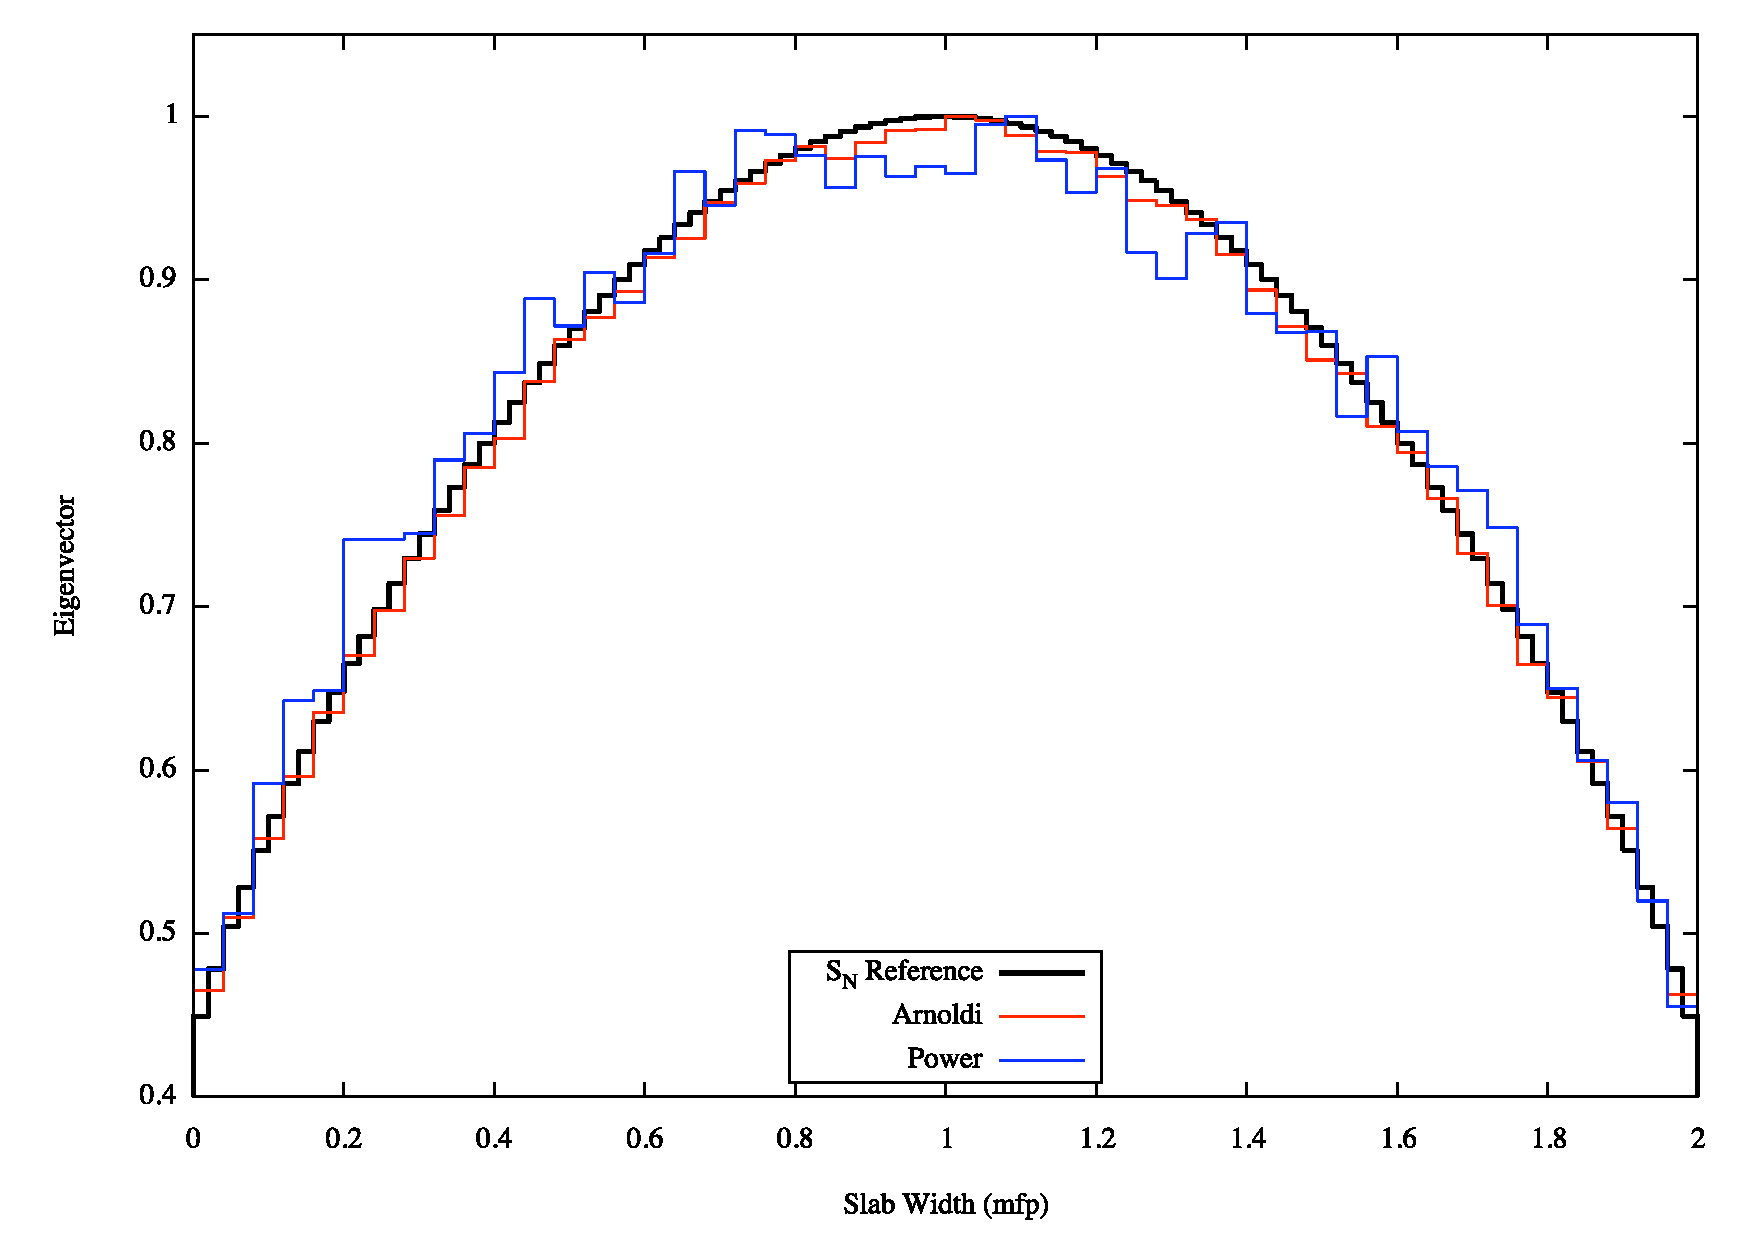
\includegraphics[width=\textwidth, keepaspectratio]{Arnoldi/Data/BasicFundamental-w2}
    % GNUPLOT: LaTeX picture with Postscript
\begingroup%
\makeatletter%
\newcommand{\GNUPLOTspecial}{%
  \@sanitize\catcode`\%=14\relax\special}%
\setlength{\unitlength}{0.0500bp}%
\begin{picture}(12960,8640)(0,0)%
  {\GNUPLOTspecial{"
%!PS-Adobe-2.0 EPSF-2.0
%%Title: BasicFundamental-w2.tex
%%Creator: gnuplot 4.3 patchlevel 0
%%CreationDate: Tue Jul 28 13:52:06 2009
%%DocumentFonts: 
%%BoundingBox: 0 0 648 432
%%EndComments
%%BeginProlog
/gnudict 256 dict def
gnudict begin
%
% The following true/false flags may be edited by hand if desired.
% The unit line width and grayscale image gamma correction may also be changed.
%
/Color true def
/Blacktext true def
/Solid true def
/Dashlength 1 def
/Landscape false def
/Level1 false def
/Rounded false def
/ClipToBoundingBox false def
/TransparentPatterns false def
/gnulinewidth 5.000 def
/userlinewidth gnulinewidth def
/Gamma 1.0 def
%
/vshift -66 def
/dl1 {
  10.0 Dashlength mul mul
  Rounded { currentlinewidth 0.75 mul sub dup 0 le { pop 0.01 } if } if
} def
/dl2 {
  10.0 Dashlength mul mul
  Rounded { currentlinewidth 0.75 mul add } if
} def
/hpt_ 31.5 def
/vpt_ 31.5 def
/hpt hpt_ def
/vpt vpt_ def
Level1 {} {
/SDict 10 dict def
systemdict /pdfmark known not {
  userdict /pdfmark systemdict /cleartomark get put
} if
SDict begin [
  /Title (BasicFundamental-w2.tex)
  /Subject (gnuplot plot)
  /Creator (gnuplot 4.3 patchlevel 0)
  /Author (Jeremy Conlin)
%  /Producer (gnuplot)
%  /Keywords ()
  /CreationDate (Tue Jul 28 13:52:06 2009)
  /DOCINFO pdfmark
end
} ifelse
/doclip {
  ClipToBoundingBox {
    newpath 0 0 moveto 648 0 lineto 648 432 lineto 0 432 lineto closepath
    clip
  } if
} def
%
% Gnuplot Prolog Version 4.2 (November 2007)
%
/M {moveto} bind def
/L {lineto} bind def
/R {rmoveto} bind def
/V {rlineto} bind def
/N {newpath moveto} bind def
/Z {closepath} bind def
/C {setrgbcolor} bind def
/f {rlineto fill} bind def
/Gshow {show} def   % May be redefined later in the file to support UTF-8
/vpt2 vpt 2 mul def
/hpt2 hpt 2 mul def
/Lshow {currentpoint stroke M 0 vshift R 
	Blacktext {gsave 0 setgray show grestore} {show} ifelse} def
/Rshow {currentpoint stroke M dup stringwidth pop neg vshift R
	Blacktext {gsave 0 setgray show grestore} {show} ifelse} def
/Cshow {currentpoint stroke M dup stringwidth pop -2 div vshift R 
	Blacktext {gsave 0 setgray show grestore} {show} ifelse} def
/UP {dup vpt_ mul /vpt exch def hpt_ mul /hpt exch def
  /hpt2 hpt 2 mul def /vpt2 vpt 2 mul def} def
/DL {Color {setrgbcolor Solid {pop []} if 0 setdash}
 {pop pop pop 0 setgray Solid {pop []} if 0 setdash} ifelse} def
/BL {stroke userlinewidth 2 mul setlinewidth
	Rounded {1 setlinejoin 1 setlinecap} if} def
/AL {stroke userlinewidth 2 div setlinewidth
	Rounded {1 setlinejoin 1 setlinecap} if} def
/UL {dup gnulinewidth mul /userlinewidth exch def
	dup 1 lt {pop 1} if 10 mul /udl exch def} def
/PL {stroke userlinewidth setlinewidth
	Rounded {1 setlinejoin 1 setlinecap} if} def
% Default Line colors
/LCw {1 1 1} def
/LCb {0 0 0} def
/LCa {0 0 0} def
/LC0 {1 0 0} def
/LC1 {0 1 0} def
/LC2 {0 0 1} def
/LC3 {1 0 1} def
/LC4 {0 1 1} def
/LC5 {1 1 0} def
/LC6 {0 0 0} def
/LC7 {1 0.3 0} def
/LC8 {0.5 0.5 0.5} def
% Default Line Types
/LTw {PL [] 1 setgray} def
/LTb {BL [] LCb DL} def
/LTa {AL [1 udl mul 2 udl mul] 0 setdash LCa setrgbcolor} def
/LT0 {PL [] LC0 DL} def
/LT1 {PL [4 dl1 2 dl2] LC1 DL} def
/LT2 {PL [2 dl1 3 dl2] LC2 DL} def
/LT3 {PL [1 dl1 1.5 dl2] LC3 DL} def
/LT4 {PL [6 dl1 2 dl2 1 dl1 2 dl2] LC4 DL} def
/LT5 {PL [3 dl1 3 dl2 1 dl1 3 dl2] LC5 DL} def
/LT6 {PL [2 dl1 2 dl2 2 dl1 6 dl2] LC6 DL} def
/LT7 {PL [1 dl1 2 dl2 6 dl1 2 dl2 1 dl1 2 dl2] LC7 DL} def
/LT8 {PL [2 dl1 2 dl2 2 dl1 2 dl2 2 dl1 2 dl2 2 dl1 4 dl2] LC8 DL} def
/Pnt {stroke [] 0 setdash gsave 1 setlinecap M 0 0 V stroke grestore} def
/Dia {stroke [] 0 setdash 2 copy vpt add M
  hpt neg vpt neg V hpt vpt neg V
  hpt vpt V hpt neg vpt V closepath stroke
  Pnt} def
/Pls {stroke [] 0 setdash vpt sub M 0 vpt2 V
  currentpoint stroke M
  hpt neg vpt neg R hpt2 0 V stroke
 } def
/Box {stroke [] 0 setdash 2 copy exch hpt sub exch vpt add M
  0 vpt2 neg V hpt2 0 V 0 vpt2 V
  hpt2 neg 0 V closepath stroke
  Pnt} def
/Crs {stroke [] 0 setdash exch hpt sub exch vpt add M
  hpt2 vpt2 neg V currentpoint stroke M
  hpt2 neg 0 R hpt2 vpt2 V stroke} def
/TriU {stroke [] 0 setdash 2 copy vpt 1.12 mul add M
  hpt neg vpt -1.62 mul V
  hpt 2 mul 0 V
  hpt neg vpt 1.62 mul V closepath stroke
  Pnt} def
/Star {2 copy Pls Crs} def
/BoxF {stroke [] 0 setdash exch hpt sub exch vpt add M
  0 vpt2 neg V hpt2 0 V 0 vpt2 V
  hpt2 neg 0 V closepath fill} def
/TriUF {stroke [] 0 setdash vpt 1.12 mul add M
  hpt neg vpt -1.62 mul V
  hpt 2 mul 0 V
  hpt neg vpt 1.62 mul V closepath fill} def
/TriD {stroke [] 0 setdash 2 copy vpt 1.12 mul sub M
  hpt neg vpt 1.62 mul V
  hpt 2 mul 0 V
  hpt neg vpt -1.62 mul V closepath stroke
  Pnt} def
/TriDF {stroke [] 0 setdash vpt 1.12 mul sub M
  hpt neg vpt 1.62 mul V
  hpt 2 mul 0 V
  hpt neg vpt -1.62 mul V closepath fill} def
/DiaF {stroke [] 0 setdash vpt add M
  hpt neg vpt neg V hpt vpt neg V
  hpt vpt V hpt neg vpt V closepath fill} def
/Pent {stroke [] 0 setdash 2 copy gsave
  translate 0 hpt M 4 {72 rotate 0 hpt L} repeat
  closepath stroke grestore Pnt} def
/PentF {stroke [] 0 setdash gsave
  translate 0 hpt M 4 {72 rotate 0 hpt L} repeat
  closepath fill grestore} def
/Circle {stroke [] 0 setdash 2 copy
  hpt 0 360 arc stroke Pnt} def
/CircleF {stroke [] 0 setdash hpt 0 360 arc fill} def
/C0 {BL [] 0 setdash 2 copy moveto vpt 90 450 arc} bind def
/C1 {BL [] 0 setdash 2 copy moveto
	2 copy vpt 0 90 arc closepath fill
	vpt 0 360 arc closepath} bind def
/C2 {BL [] 0 setdash 2 copy moveto
	2 copy vpt 90 180 arc closepath fill
	vpt 0 360 arc closepath} bind def
/C3 {BL [] 0 setdash 2 copy moveto
	2 copy vpt 0 180 arc closepath fill
	vpt 0 360 arc closepath} bind def
/C4 {BL [] 0 setdash 2 copy moveto
	2 copy vpt 180 270 arc closepath fill
	vpt 0 360 arc closepath} bind def
/C5 {BL [] 0 setdash 2 copy moveto
	2 copy vpt 0 90 arc
	2 copy moveto
	2 copy vpt 180 270 arc closepath fill
	vpt 0 360 arc} bind def
/C6 {BL [] 0 setdash 2 copy moveto
	2 copy vpt 90 270 arc closepath fill
	vpt 0 360 arc closepath} bind def
/C7 {BL [] 0 setdash 2 copy moveto
	2 copy vpt 0 270 arc closepath fill
	vpt 0 360 arc closepath} bind def
/C8 {BL [] 0 setdash 2 copy moveto
	2 copy vpt 270 360 arc closepath fill
	vpt 0 360 arc closepath} bind def
/C9 {BL [] 0 setdash 2 copy moveto
	2 copy vpt 270 450 arc closepath fill
	vpt 0 360 arc closepath} bind def
/C10 {BL [] 0 setdash 2 copy 2 copy moveto vpt 270 360 arc closepath fill
	2 copy moveto
	2 copy vpt 90 180 arc closepath fill
	vpt 0 360 arc closepath} bind def
/C11 {BL [] 0 setdash 2 copy moveto
	2 copy vpt 0 180 arc closepath fill
	2 copy moveto
	2 copy vpt 270 360 arc closepath fill
	vpt 0 360 arc closepath} bind def
/C12 {BL [] 0 setdash 2 copy moveto
	2 copy vpt 180 360 arc closepath fill
	vpt 0 360 arc closepath} bind def
/C13 {BL [] 0 setdash 2 copy moveto
	2 copy vpt 0 90 arc closepath fill
	2 copy moveto
	2 copy vpt 180 360 arc closepath fill
	vpt 0 360 arc closepath} bind def
/C14 {BL [] 0 setdash 2 copy moveto
	2 copy vpt 90 360 arc closepath fill
	vpt 0 360 arc} bind def
/C15 {BL [] 0 setdash 2 copy vpt 0 360 arc closepath fill
	vpt 0 360 arc closepath} bind def
/Rec {newpath 4 2 roll moveto 1 index 0 rlineto 0 exch rlineto
	neg 0 rlineto closepath} bind def
/Square {dup Rec} bind def
/Bsquare {vpt sub exch vpt sub exch vpt2 Square} bind def
/S0 {BL [] 0 setdash 2 copy moveto 0 vpt rlineto BL Bsquare} bind def
/S1 {BL [] 0 setdash 2 copy vpt Square fill Bsquare} bind def
/S2 {BL [] 0 setdash 2 copy exch vpt sub exch vpt Square fill Bsquare} bind def
/S3 {BL [] 0 setdash 2 copy exch vpt sub exch vpt2 vpt Rec fill Bsquare} bind def
/S4 {BL [] 0 setdash 2 copy exch vpt sub exch vpt sub vpt Square fill Bsquare} bind def
/S5 {BL [] 0 setdash 2 copy 2 copy vpt Square fill
	exch vpt sub exch vpt sub vpt Square fill Bsquare} bind def
/S6 {BL [] 0 setdash 2 copy exch vpt sub exch vpt sub vpt vpt2 Rec fill Bsquare} bind def
/S7 {BL [] 0 setdash 2 copy exch vpt sub exch vpt sub vpt vpt2 Rec fill
	2 copy vpt Square fill Bsquare} bind def
/S8 {BL [] 0 setdash 2 copy vpt sub vpt Square fill Bsquare} bind def
/S9 {BL [] 0 setdash 2 copy vpt sub vpt vpt2 Rec fill Bsquare} bind def
/S10 {BL [] 0 setdash 2 copy vpt sub vpt Square fill 2 copy exch vpt sub exch vpt Square fill
	Bsquare} bind def
/S11 {BL [] 0 setdash 2 copy vpt sub vpt Square fill 2 copy exch vpt sub exch vpt2 vpt Rec fill
	Bsquare} bind def
/S12 {BL [] 0 setdash 2 copy exch vpt sub exch vpt sub vpt2 vpt Rec fill Bsquare} bind def
/S13 {BL [] 0 setdash 2 copy exch vpt sub exch vpt sub vpt2 vpt Rec fill
	2 copy vpt Square fill Bsquare} bind def
/S14 {BL [] 0 setdash 2 copy exch vpt sub exch vpt sub vpt2 vpt Rec fill
	2 copy exch vpt sub exch vpt Square fill Bsquare} bind def
/S15 {BL [] 0 setdash 2 copy Bsquare fill Bsquare} bind def
/D0 {gsave translate 45 rotate 0 0 S0 stroke grestore} bind def
/D1 {gsave translate 45 rotate 0 0 S1 stroke grestore} bind def
/D2 {gsave translate 45 rotate 0 0 S2 stroke grestore} bind def
/D3 {gsave translate 45 rotate 0 0 S3 stroke grestore} bind def
/D4 {gsave translate 45 rotate 0 0 S4 stroke grestore} bind def
/D5 {gsave translate 45 rotate 0 0 S5 stroke grestore} bind def
/D6 {gsave translate 45 rotate 0 0 S6 stroke grestore} bind def
/D7 {gsave translate 45 rotate 0 0 S7 stroke grestore} bind def
/D8 {gsave translate 45 rotate 0 0 S8 stroke grestore} bind def
/D9 {gsave translate 45 rotate 0 0 S9 stroke grestore} bind def
/D10 {gsave translate 45 rotate 0 0 S10 stroke grestore} bind def
/D11 {gsave translate 45 rotate 0 0 S11 stroke grestore} bind def
/D12 {gsave translate 45 rotate 0 0 S12 stroke grestore} bind def
/D13 {gsave translate 45 rotate 0 0 S13 stroke grestore} bind def
/D14 {gsave translate 45 rotate 0 0 S14 stroke grestore} bind def
/D15 {gsave translate 45 rotate 0 0 S15 stroke grestore} bind def
/DiaE {stroke [] 0 setdash vpt add M
  hpt neg vpt neg V hpt vpt neg V
  hpt vpt V hpt neg vpt V closepath stroke} def
/BoxE {stroke [] 0 setdash exch hpt sub exch vpt add M
  0 vpt2 neg V hpt2 0 V 0 vpt2 V
  hpt2 neg 0 V closepath stroke} def
/TriUE {stroke [] 0 setdash vpt 1.12 mul add M
  hpt neg vpt -1.62 mul V
  hpt 2 mul 0 V
  hpt neg vpt 1.62 mul V closepath stroke} def
/TriDE {stroke [] 0 setdash vpt 1.12 mul sub M
  hpt neg vpt 1.62 mul V
  hpt 2 mul 0 V
  hpt neg vpt -1.62 mul V closepath stroke} def
/PentE {stroke [] 0 setdash gsave
  translate 0 hpt M 4 {72 rotate 0 hpt L} repeat
  closepath stroke grestore} def
/CircE {stroke [] 0 setdash 
  hpt 0 360 arc stroke} def
/Opaque {gsave closepath 1 setgray fill grestore 0 setgray closepath} def
/DiaW {stroke [] 0 setdash vpt add M
  hpt neg vpt neg V hpt vpt neg V
  hpt vpt V hpt neg vpt V Opaque stroke} def
/BoxW {stroke [] 0 setdash exch hpt sub exch vpt add M
  0 vpt2 neg V hpt2 0 V 0 vpt2 V
  hpt2 neg 0 V Opaque stroke} def
/TriUW {stroke [] 0 setdash vpt 1.12 mul add M
  hpt neg vpt -1.62 mul V
  hpt 2 mul 0 V
  hpt neg vpt 1.62 mul V Opaque stroke} def
/TriDW {stroke [] 0 setdash vpt 1.12 mul sub M
  hpt neg vpt 1.62 mul V
  hpt 2 mul 0 V
  hpt neg vpt -1.62 mul V Opaque stroke} def
/PentW {stroke [] 0 setdash gsave
  translate 0 hpt M 4 {72 rotate 0 hpt L} repeat
  Opaque stroke grestore} def
/CircW {stroke [] 0 setdash 
  hpt 0 360 arc Opaque stroke} def
/BoxFill {gsave Rec 1 setgray fill grestore} def
/Density {
  /Fillden exch def
  currentrgbcolor
  /ColB exch def /ColG exch def /ColR exch def
  /ColR ColR Fillden mul Fillden sub 1 add def
  /ColG ColG Fillden mul Fillden sub 1 add def
  /ColB ColB Fillden mul Fillden sub 1 add def
  ColR ColG ColB setrgbcolor} def
/BoxColFill {gsave Rec PolyFill} def
/PolyFill {gsave Density fill grestore grestore} def
/h {rlineto rlineto rlineto gsave closepath fill grestore} bind def
%
% PostScript Level 1 Pattern Fill routine for rectangles
% Usage: x y w h s a XX PatternFill
%	x,y = lower left corner of box to be filled
%	w,h = width and height of box
%	  a = angle in degrees between lines and x-axis
%	 XX = 0/1 for no/yes cross-hatch
%
/PatternFill {gsave /PFa [ 9 2 roll ] def
  PFa 0 get PFa 2 get 2 div add PFa 1 get PFa 3 get 2 div add translate
  PFa 2 get -2 div PFa 3 get -2 div PFa 2 get PFa 3 get Rec
  gsave 1 setgray fill grestore clip
  currentlinewidth 0.5 mul setlinewidth
  /PFs PFa 2 get dup mul PFa 3 get dup mul add sqrt def
  0 0 M PFa 5 get rotate PFs -2 div dup translate
  0 1 PFs PFa 4 get div 1 add floor cvi
	{PFa 4 get mul 0 M 0 PFs V} for
  0 PFa 6 get ne {
	0 1 PFs PFa 4 get div 1 add floor cvi
	{PFa 4 get mul 0 2 1 roll M PFs 0 V} for
 } if
  stroke grestore} def
%
/languagelevel where
 {pop languagelevel} {1} ifelse
 2 lt
	{/InterpretLevel1 true def}
	{/InterpretLevel1 Level1 def}
 ifelse
%
% PostScript level 2 pattern fill definitions
%
/Level2PatternFill {
/Tile8x8 {/PaintType 2 /PatternType 1 /TilingType 1 /BBox [0 0 8 8] /XStep 8 /YStep 8}
	bind def
/KeepColor {currentrgbcolor [/Pattern /DeviceRGB] setcolorspace} bind def
<< Tile8x8
 /PaintProc {0.5 setlinewidth pop 0 0 M 8 8 L 0 8 M 8 0 L stroke} 
>> matrix makepattern
/Pat1 exch def
<< Tile8x8
 /PaintProc {0.5 setlinewidth pop 0 0 M 8 8 L 0 8 M 8 0 L stroke
	0 4 M 4 8 L 8 4 L 4 0 L 0 4 L stroke}
>> matrix makepattern
/Pat2 exch def
<< Tile8x8
 /PaintProc {0.5 setlinewidth pop 0 0 M 0 8 L
	8 8 L 8 0 L 0 0 L fill}
>> matrix makepattern
/Pat3 exch def
<< Tile8x8
 /PaintProc {0.5 setlinewidth pop -4 8 M 8 -4 L
	0 12 M 12 0 L stroke}
>> matrix makepattern
/Pat4 exch def
<< Tile8x8
 /PaintProc {0.5 setlinewidth pop -4 0 M 8 12 L
	0 -4 M 12 8 L stroke}
>> matrix makepattern
/Pat5 exch def
<< Tile8x8
 /PaintProc {0.5 setlinewidth pop -2 8 M 4 -4 L
	0 12 M 8 -4 L 4 12 M 10 0 L stroke}
>> matrix makepattern
/Pat6 exch def
<< Tile8x8
 /PaintProc {0.5 setlinewidth pop -2 0 M 4 12 L
	0 -4 M 8 12 L 4 -4 M 10 8 L stroke}
>> matrix makepattern
/Pat7 exch def
<< Tile8x8
 /PaintProc {0.5 setlinewidth pop 8 -2 M -4 4 L
	12 0 M -4 8 L 12 4 M 0 10 L stroke}
>> matrix makepattern
/Pat8 exch def
<< Tile8x8
 /PaintProc {0.5 setlinewidth pop 0 -2 M 12 4 L
	-4 0 M 12 8 L -4 4 M 8 10 L stroke}
>> matrix makepattern
/Pat9 exch def
/Pattern1 {PatternBgnd KeepColor Pat1 setpattern} bind def
/Pattern2 {PatternBgnd KeepColor Pat2 setpattern} bind def
/Pattern3 {PatternBgnd KeepColor Pat3 setpattern} bind def
/Pattern4 {PatternBgnd KeepColor Landscape {Pat5} {Pat4} ifelse setpattern} bind def
/Pattern5 {PatternBgnd KeepColor Landscape {Pat4} {Pat5} ifelse setpattern} bind def
/Pattern6 {PatternBgnd KeepColor Landscape {Pat9} {Pat6} ifelse setpattern} bind def
/Pattern7 {PatternBgnd KeepColor Landscape {Pat8} {Pat7} ifelse setpattern} bind def
} def
%
%
%End of PostScript Level 2 code
%
/PatternBgnd {
  TransparentPatterns {} {gsave 1 setgray fill grestore} ifelse
} def
%
% Substitute for Level 2 pattern fill codes with
% grayscale if Level 2 support is not selected.
%
/Level1PatternFill {
/Pattern1 {0.250 Density} bind def
/Pattern2 {0.500 Density} bind def
/Pattern3 {0.750 Density} bind def
/Pattern4 {0.125 Density} bind def
/Pattern5 {0.375 Density} bind def
/Pattern6 {0.625 Density} bind def
/Pattern7 {0.875 Density} bind def
} def
%
% Now test for support of Level 2 code
%
Level1 {Level1PatternFill} {Level2PatternFill} ifelse
%
/Symbol-Oblique /Symbol findfont [1 0 .167 1 0 0] makefont
dup length dict begin {1 index /FID eq {pop pop} {def} ifelse} forall
currentdict end definefont pop
end
%%EndProlog
gnudict begin
gsave
doclip
0 0 translate
0.050 0.050 scale
0 setgray
newpath
1.000 UL
LTb
1100 640 M
63 0 V
11396 0 R
-63 0 V
1100 1834 M
63 0 V
11396 0 R
-63 0 V
1100 3027 M
63 0 V
11396 0 R
-63 0 V
1100 4221 M
63 0 V
11396 0 R
-63 0 V
1100 5415 M
63 0 V
11396 0 R
-63 0 V
1100 6608 M
63 0 V
11396 0 R
-63 0 V
1100 7802 M
63 0 V
11396 0 R
-63 0 V
1100 640 M
0 63 V
0 7696 R
0 -63 V
2246 640 M
0 63 V
0 7696 R
0 -63 V
3392 640 M
0 63 V
0 7696 R
0 -63 V
4538 640 M
0 63 V
0 7696 R
0 -63 V
5684 640 M
0 63 V
0 7696 R
0 -63 V
6830 640 M
0 63 V
0 7696 R
0 -63 V
7975 640 M
0 63 V
0 7696 R
0 -63 V
9121 640 M
0 63 V
0 7696 R
0 -63 V
10267 640 M
0 63 V
0 7696 R
0 -63 V
11413 640 M
0 63 V
0 7696 R
0 -63 V
12559 640 M
0 63 V
0 7696 R
0 -63 V
stroke
1100 8399 N
0 -7759 V
11459 0 V
0 7759 V
-11459 0 V
Z stroke
LCb setrgbcolor
LTb
LCb setrgbcolor
LTb
LCb setrgbcolor
LTb
LCb setrgbcolor
LTb
1.000 UP
1.000 UL
LTb
1.000 UL
LTb
5658 703 N
0 800 V
2342 0 V
0 -800 V
-2342 0 V
Z stroke
5658 1503 M
2342 0 V
stroke
2.000 UL
LTb
LCb setrgbcolor
LTb
7338 1303 M
543 0 V
1100 640 M
0 591 V
115 0 V
0 344 V
114 0 V
0 311 V
115 0 V
0 286 V
114 0 V
0 266 V
115 0 V
0 253 V
115 0 V
0 240 V
114 0 V
0 229 V
115 0 V
0 222 V
114 0 V
0 214 V
115 0 V
0 208 V
114 0 V
0 201 V
115 0 V
0 195 V
115 0 V
0 189 V
114 0 V
0 184 V
115 0 V
0 178 V
114 0 V
0 174 V
115 0 V
0 168 V
115 0 V
0 163 V
114 0 V
0 158 V
115 0 V
0 152 V
114 0 V
0 148 V
115 0 V
0 143 V
115 0 V
0 138 V
114 0 V
0 132 V
115 0 V
0 128 V
114 0 V
0 123 V
115 0 V
0 118 V
115 0 V
0 113 V
114 0 V
0 108 V
115 0 V
0 103 V
114 0 V
0 97 V
115 0 V
0 93 V
114 0 V
0 87 V
115 0 V
0 83 V
115 0 V
0 77 V
114 0 V
0 73 V
115 0 V
0 67 V
114 0 V
0 62 V
115 0 V
0 57 V
115 0 V
0 52 V
114 0 V
0 47 V
115 0 V
0 41 V
114 0 V
0 37 V
115 0 V
0 31 V
115 0 V
0 26 V
114 0 V
0 21 V
115 0 V
0 15 V
114 0 V
0 11 V
115 0 V
0 5 V
172 0 V
0 -5 V
172 0 V
stroke 7059 7797 M
0 -11 V
114 0 V
0 -15 V
115 0 V
0 -21 V
114 0 V
0 -26 V
115 0 V
0 -31 V
115 0 V
0 -37 V
114 0 V
0 -41 V
115 0 V
0 -47 V
114 0 V
0 -52 V
115 0 V
0 -57 V
115 0 V
0 -62 V
114 0 V
0 -67 V
115 0 V
0 -73 V
114 0 V
0 -77 V
115 0 V
0 -83 V
115 0 V
0 -87 V
114 0 V
0 -93 V
115 0 V
0 -97 V
114 0 V
0 -103 V
115 0 V
0 -108 V
114 0 V
0 -113 V
115 0 V
0 -118 V
115 0 V
0 -123 V
114 0 V
0 -128 V
115 0 V
0 -132 V
114 0 V
0 -138 V
115 0 V
0 -143 V
115 0 V
0 -148 V
114 0 V
0 -152 V
115 0 V
0 -158 V
114 0 V
0 -163 V
115 0 V
0 -168 V
115 0 V
0 -174 V
114 0 V
0 -178 V
115 0 V
0 -184 V
114 0 V
0 -189 V
115 0 V
0 -195 V
115 0 V
0 -201 V
114 0 V
0 -208 V
115 0 V
0 -214 V
114 0 V
0 -222 V
115 0 V
0 -229 V
114 0 V
0 -240 V
115 0 V
0 -253 V
115 0 V
0 -266 V
114 0 V
0 -286 V
115 0 V
0 -311 V
114 0 V
0 -344 V
115 0 V
0 -591 V
stroke
1.000 UL
LT0
LCb setrgbcolor
LT0
7338 1103 M
543 0 V
1100 1318 M
153 0 V
0 446 V
153 0 V
0 371 V
152 0 V
0 338 V
153 0 V
0 332 V
153 0 V
0 309 V
153 0 V
0 320 V
152 0 V
0 277 V
153 0 V
0 261 V
153 0 V
0 266 V
153 0 V
0 255 V
153 0 V
0 218 V
152 0 V
0 250 V
153 0 V
0 215 V
153 0 V
0 216 V
153 0 V
0 197 V
153 0 V
0 216 V
152 0 V
0 175 V
153 0 V
0 178 V
153 0 V
0 169 V
153 0 V
0 141 V
153 0 V
0 166 V
152 0 V
0 135 V
153 0 V
0 133 V
153 0 V
0 116 V
153 0 V
0 145 V
152 0 V
0 83 V
153 0 V
0 102 V
153 0 V
0 73 V
153 0 V
0 92 V
153 0 V
0 80 V
152 0 V
0 63 V
153 0 V
0 46 V
153 0 V
0 51 V
153 0 V
0 31 V
153 0 V
0 1 V
152 0 V
0 14 V
153 0 V
0 3 V
153 0 V
0 -7 V
153 0 V
0 -5 V
152 0 V
0 -23 V
153 0 V
0 -25 V
153 0 V
0 -44 V
153 0 V
0 -57 V
153 0 V
0 -65 V
152 0 V
0 -72 V
153 0 V
0 -63 V
153 0 V
0 -102 V
153 0 V
0 -93 V
152 0 V
0 -110 V
153 0 V
0 -90 V
153 0 V
0 -134 V
stroke 8892 6912 M
153 0 V
0 -131 V
153 0 V
0 -163 V
152 0 V
0 -159 V
153 0 V
0 -131 V
153 0 V
0 -180 V
153 0 V
0 -175 V
153 0 V
0 -177 V
153 0 V
0 -206 V
152 0 V
0 -192 V
153 0 V
0 -210 V
153 0 V
0 -234 V
153 0 V
0 -240 V
152 0 V
0 -222 V
153 0 V
0 -261 V
153 0 V
0 -250 V
153 0 V
0 -279 V
153 0 V
0 -289 V
152 0 V
0 -288 V
153 0 V
0 -299 V
153 0 V
0 -326 V
153 0 V
0 -354 V
152 0 V
0 -390 V
153 0 V
0 -431 V
153 0 V
stroke
LT2
LCb setrgbcolor
LT2
7338 903 M
543 0 V
1100 1304 M
153 0 V
0 435 V
153 0 V
0 372 V
152 0 V
0 380 V
153 0 V
0 305 V
153 0 V
0 304 V
153 0 V
0 294 V
152 0 V
0 290 V
153 0 V
0 261 V
153 0 V
0 284 V
153 0 V
0 251 V
153 0 V
0 219 V
152 0 V
0 231 V
153 0 V
0 223 V
153 0 V
0 220 V
153 0 V
0 182 V
153 0 V
0 242 V
152 0 V
0 188 V
153 0 V
0 131 V
153 0 V
0 205 V
153 0 V
0 153 V
153 0 V
0 122 V
152 0 V
0 163 V
153 0 V
0 84 V
153 0 V
0 164 V
153 0 V
0 111 V
152 0 V
0 95 V
153 0 V
0 142 V
153 0 V
0 41 V
153 0 V
0 84 V
153 0 V
0 79 V
152 0 V
0 43 V
153 0 V
0 78 V
153 0 V
0 1 V
153 0 V
0 65 V
153 0 V
0 29 V
152 0 V
0 5 V
153 0 V
0 22 V
153 0 V
0 -19 V
153 0 V
152 0 V
0 -42 V
153 0 V
0 -42 V
153 0 V
0 -19 V
153 0 V
0 -90 V
153 0 V
0 -33 V
152 0 V
0 -66 V
153 0 V
0 -64 V
153 0 V
0 -80 V
153 0 V
0 -132 V
152 0 V
0 -83 V
153 0 V
0 -106 V
153 0 V
0 -127 V
153 0 V
stroke 9045 6899 M
0 -115 V
153 0 V
0 -167 V
152 0 V
0 -170 V
153 0 V
0 -148 V
153 0 V
0 -169 V
153 0 V
0 -208 V
153 0 V
0 -174 V
153 0 V
0 -198 V
152 0 V
0 -165 V
153 0 V
0 -206 V
153 0 V
0 -207 V
153 0 V
0 -287 V
152 0 V
0 -211 V
153 0 V
0 -250 V
153 0 V
0 -264 V
153 0 V
0 -261 V
153 0 V
0 -278 V
152 0 V
0 -313 V
153 0 V
0 -299 V
153 0 V
0 -312 V
153 0 V
0 -347 V
152 0 V
0 -411 V
153 0 V
0 -416 V
153 0 V
stroke
LTb
1100 8399 N
0 -7759 V
11459 0 V
0 7759 V
-11459 0 V
Z stroke
1.000 UP
1.000 UL
LTb
stroke
grestore
end
showpage
  }}%
  \put(7218,903){\makebox(0,0)[r]{\strut{}Arnoldi}}%
  \put(7218,1103){\makebox(0,0)[r]{\strut{}Power}}%
  \put(7218,1303){\makebox(0,0)[r]{\strut{}$S_N$ Reference}}%
  \put(6829,140){\makebox(0,0){\strut{}Slab Width (mfp)}}%
  \put(280,4519){%
  \special{ps: gsave currentpoint currentpoint translate
270 rotate neg exch neg exch translate}%
  \makebox(0,0){\strut{}Eigenvector}%
  \special{ps: currentpoint grestore moveto}%
  }%
  \put(12559,440){\makebox(0,0){\strut{} 2}}%
  \put(11413,440){\makebox(0,0){\strut{} 1.8}}%
  \put(10267,440){\makebox(0,0){\strut{} 1.6}}%
  \put(9121,440){\makebox(0,0){\strut{} 1.4}}%
  \put(7975,440){\makebox(0,0){\strut{} 1.2}}%
  \put(6830,440){\makebox(0,0){\strut{} 1}}%
  \put(5684,440){\makebox(0,0){\strut{} 0.8}}%
  \put(4538,440){\makebox(0,0){\strut{} 0.6}}%
  \put(3392,440){\makebox(0,0){\strut{} 0.4}}%
  \put(2246,440){\makebox(0,0){\strut{} 0.2}}%
  \put(1100,440){\makebox(0,0){\strut{} 0}}%
  \put(980,7802){\makebox(0,0)[r]{\strut{} 1}}%
  \put(980,6608){\makebox(0,0)[r]{\strut{} 0.9}}%
  \put(980,5415){\makebox(0,0)[r]{\strut{} 0.8}}%
  \put(980,4221){\makebox(0,0)[r]{\strut{} 0.7}}%
  \put(980,3027){\makebox(0,0)[r]{\strut{} 0.6}}%
  \put(980,1834){\makebox(0,0)[r]{\strut{} 0.5}}%
  \put(980,640){\makebox(0,0)[r]{\strut{} 0.4}}%
\end{picture}%
\endgroup
\endinput

    \caption{Fundamental eigenvector estimates from the power method and Arnoldi's method for the 2.0 mfp wide slab.  The heavy line shows the S$_\mathrm{N}$ solution.}
    \label{fig:BasicFundamentalW2}
\end{sidewaysfigure}
\end{comment}

\clearpage
\subsection{Discretization Error \label{sec:DiscretizationBias}} 

One of the benefits of Monte Carlo particle transport is the ability to use exact geometry without discretization.  This is true for the transport of particles in the power method, but the fission source must be discretized for tallying.  Arnoldi's method, on the other hand, must have a discretized source  in order to orthogonalize the Arnoldi vectors, as described in \Fref{sec:SpatialDiscretization}.

The discretization of the fission source can lead to an error in the estimated eigenvalue if an insufficient number of spatial bins are used to represent the fission source.  To illustrate this effect a series of simulations is shown using the same slab of multiplying material with varying number of spatial bins.  The slab here is exactly the same as for the 20 mfp problem shown earlier (\mbox{$\nu\Sigma_f = 1.0$}, \mbox{$\Sigma_a = 0.2$}, \mbox{$\Sigma_s = 0.8$} with \mbox{$\Sigma_t = 1.0$}).  This time $10^5$ histories are tracked per iteration with 50 inactive restarts and 500 active restarts.  The increase in the number of histories and restarts is to reduce the statistical uncertainty to ensure the error can be seen outside the noise.  This simulation was performed eleven times varying the number of spatial discretization bins from 10 to 150.  

The results of these simulations are shown in \Fref{tab:Discretization} for the fundamental eigenvalue.  We can see that the uncertainty in the eigenvalue estimate (standard deviation) is relatively independent of the number of spatial bins.  The error in the eigenvalue estimate is the absolute value of the difference between the eigenvalue estimate and the reference solution.  We see that the error in the eigenvalue estimate is larger than the statistical uncertainty for bin widths \mbox{$\leq 0.5$} mfp thick.  For bin widths greater than 0.5 mfp thick the error is less than the statistical uncertainty. 

The data from \Fref{tab:Discretization} is shown graphically in \Fref{fig:BasicBias}.  The error in the eigenvalue estimate for the first two harmonics are also shown in \Fref{fig:BasicBias}.  The error in the eigenvalue estimate is denoted marked as $\mathcal{B}$ for each of the eigenvalue estimates.  Best fit lines are drawn through the points on the graph.  We see that there is a very good linear fit to these data points.  

\begin{table}[h] \centering
    \begin{tabular}{cccccc}
        \toprule
        \# of Bins & Bin Width (mfp) & Eigenvalue & Uncertainty & Error & FOM\\
        \midrule
         10 & 2.00 & 4.8003 & 6.6\e{-4} & 2.7\e{-2} & 831.2 \\
         25 & 0.80 & 4.8224 & 6.8\e{-4} & 5.3\e{-3} & 773.2 \\
         40 & 0.50 & 4.8251 & 6.3\e{-4} & 2.6\e{-3} & 872.0 \\
         50 & 0.40 & 4.8273 & 6.5\e{-4} & 4.2\e{-4} & 829.0 \\
         60 & 0.33 & 4.8258 & 6.9\e{-4} & 2.0\e{-3} & 704.3 \\
         75 & 0.27 & 4.8275 & 6.7\e{-4} & 2.4\e{-4} & 753.0 \\
         90 & 0.22 & 4.8277 & 6.7\e{-4} & 4.2\e{-5} & 746.1 \\
        105 & 0.19 & 4.8277 & 6.9\e{-4} & 5.2\e{-5} & 698.3 \\
        120 & 0.17 & 4.8282 & 6.5\e{-4} & 4.1\e{-4} & 767.8 \\
        135 & 0.15 & 4.8274 & 7.0\e{-4} & 3.1\e{-4} & 656.9 \\
        150 & 0.13 & 4.8285 & 6.4\e{-4} & 7.5\e{-4} & 792.0 \\
        \bottomrule
    \end{tabular}
    \caption{Eigenvalue estimates of the fundamental eigenvalue from Arnoldi's method and the error in the estimate.  The error is the difference between the estimate and the reference value ($\lambda_0 = 4.8278$, see \cite{Garis:1991One-s-0} and \cite{Dahl:1979Eigen-0}).}
    \label{tab:Discretization}
\end{table}

\begin{sidewaysfigure}[h] \centering
    % GNUPLOT: LaTeX picture with Postscript
\begingroup%
\makeatletter%
\newcommand{\GNUPLOTspecial}{%
  \@sanitize\catcode`\%=14\relax\special}%
\setlength{\unitlength}{0.0500bp}%
\begin{picture}(8640,6480)(0,0)%
  {\GNUPLOTspecial{"
%!PS-Adobe-2.0 EPSF-2.0
%%Title: BiasHistogram.tex
%%Creator: gnuplot 4.3 patchlevel 0
%%CreationDate: Wed Aug 12 16:28:22 2009
%%DocumentFonts: 
%%BoundingBox: 0 0 432 324
%%EndComments
%%BeginProlog
/gnudict 256 dict def
gnudict begin
%
% The following true/false flags may be edited by hand if desired.
% The unit line width and grayscale image gamma correction may also be changed.
%
/Color true def
/Blacktext true def
/Solid true def
/Dashlength 1 def
/Landscape false def
/Level1 false def
/Rounded false def
/ClipToBoundingBox false def
/TransparentPatterns false def
/gnulinewidth 5.000 def
/userlinewidth gnulinewidth def
/Gamma 1.0 def
%
/vshift -66 def
/dl1 {
  10.0 Dashlength mul mul
  Rounded { currentlinewidth 0.75 mul sub dup 0 le { pop 0.01 } if } if
} def
/dl2 {
  10.0 Dashlength mul mul
  Rounded { currentlinewidth 0.75 mul add } if
} def
/hpt_ 31.5 def
/vpt_ 31.5 def
/hpt hpt_ def
/vpt vpt_ def
Level1 {} {
/SDict 10 dict def
systemdict /pdfmark known not {
  userdict /pdfmark systemdict /cleartomark get put
} if
SDict begin [
  /Title (BiasHistogram.tex)
  /Subject (gnuplot plot)
  /Creator (gnuplot 4.3 patchlevel 0)
  /Author (Jeremy Conlin)
%  /Producer (gnuplot)
%  /Keywords ()
  /CreationDate (Wed Aug 12 16:28:22 2009)
  /DOCINFO pdfmark
end
} ifelse
/doclip {
  ClipToBoundingBox {
    newpath 0 0 moveto 432 0 lineto 432 324 lineto 0 324 lineto closepath
    clip
  } if
} def
%
% Gnuplot Prolog Version 4.2 (November 2007)
%
/M {moveto} bind def
/L {lineto} bind def
/R {rmoveto} bind def
/V {rlineto} bind def
/N {newpath moveto} bind def
/Z {closepath} bind def
/C {setrgbcolor} bind def
/f {rlineto fill} bind def
/Gshow {show} def   % May be redefined later in the file to support UTF-8
/vpt2 vpt 2 mul def
/hpt2 hpt 2 mul def
/Lshow {currentpoint stroke M 0 vshift R 
	Blacktext {gsave 0 setgray show grestore} {show} ifelse} def
/Rshow {currentpoint stroke M dup stringwidth pop neg vshift R
	Blacktext {gsave 0 setgray show grestore} {show} ifelse} def
/Cshow {currentpoint stroke M dup stringwidth pop -2 div vshift R 
	Blacktext {gsave 0 setgray show grestore} {show} ifelse} def
/UP {dup vpt_ mul /vpt exch def hpt_ mul /hpt exch def
  /hpt2 hpt 2 mul def /vpt2 vpt 2 mul def} def
/DL {Color {setrgbcolor Solid {pop []} if 0 setdash}
 {pop pop pop 0 setgray Solid {pop []} if 0 setdash} ifelse} def
/BL {stroke userlinewidth 2 mul setlinewidth
	Rounded {1 setlinejoin 1 setlinecap} if} def
/AL {stroke userlinewidth 2 div setlinewidth
	Rounded {1 setlinejoin 1 setlinecap} if} def
/UL {dup gnulinewidth mul /userlinewidth exch def
	dup 1 lt {pop 1} if 10 mul /udl exch def} def
/PL {stroke userlinewidth setlinewidth
	Rounded {1 setlinejoin 1 setlinecap} if} def
% Default Line colors
/LCw {1 1 1} def
/LCb {0 0 0} def
/LCa {0 0 0} def
/LC0 {1 0 0} def
/LC1 {0 1 0} def
/LC2 {0 0 1} def
/LC3 {1 0 1} def
/LC4 {0 1 1} def
/LC5 {1 1 0} def
/LC6 {0 0 0} def
/LC7 {1 0.3 0} def
/LC8 {0.5 0.5 0.5} def
% Default Line Types
/LTw {PL [] 1 setgray} def
/LTb {BL [] LCb DL} def
/LTa {AL [1 udl mul 2 udl mul] 0 setdash LCa setrgbcolor} def
/LT0 {PL [] LC0 DL} def
/LT1 {PL [4 dl1 2 dl2] LC1 DL} def
/LT2 {PL [2 dl1 3 dl2] LC2 DL} def
/LT3 {PL [1 dl1 1.5 dl2] LC3 DL} def
/LT4 {PL [6 dl1 2 dl2 1 dl1 2 dl2] LC4 DL} def
/LT5 {PL [3 dl1 3 dl2 1 dl1 3 dl2] LC5 DL} def
/LT6 {PL [2 dl1 2 dl2 2 dl1 6 dl2] LC6 DL} def
/LT7 {PL [1 dl1 2 dl2 6 dl1 2 dl2 1 dl1 2 dl2] LC7 DL} def
/LT8 {PL [2 dl1 2 dl2 2 dl1 2 dl2 2 dl1 2 dl2 2 dl1 4 dl2] LC8 DL} def
/Pnt {stroke [] 0 setdash gsave 1 setlinecap M 0 0 V stroke grestore} def
/Dia {stroke [] 0 setdash 2 copy vpt add M
  hpt neg vpt neg V hpt vpt neg V
  hpt vpt V hpt neg vpt V closepath stroke
  Pnt} def
/Pls {stroke [] 0 setdash vpt sub M 0 vpt2 V
  currentpoint stroke M
  hpt neg vpt neg R hpt2 0 V stroke
 } def
/Box {stroke [] 0 setdash 2 copy exch hpt sub exch vpt add M
  0 vpt2 neg V hpt2 0 V 0 vpt2 V
  hpt2 neg 0 V closepath stroke
  Pnt} def
/Crs {stroke [] 0 setdash exch hpt sub exch vpt add M
  hpt2 vpt2 neg V currentpoint stroke M
  hpt2 neg 0 R hpt2 vpt2 V stroke} def
/TriU {stroke [] 0 setdash 2 copy vpt 1.12 mul add M
  hpt neg vpt -1.62 mul V
  hpt 2 mul 0 V
  hpt neg vpt 1.62 mul V closepath stroke
  Pnt} def
/Star {2 copy Pls Crs} def
/BoxF {stroke [] 0 setdash exch hpt sub exch vpt add M
  0 vpt2 neg V hpt2 0 V 0 vpt2 V
  hpt2 neg 0 V closepath fill} def
/TriUF {stroke [] 0 setdash vpt 1.12 mul add M
  hpt neg vpt -1.62 mul V
  hpt 2 mul 0 V
  hpt neg vpt 1.62 mul V closepath fill} def
/TriD {stroke [] 0 setdash 2 copy vpt 1.12 mul sub M
  hpt neg vpt 1.62 mul V
  hpt 2 mul 0 V
  hpt neg vpt -1.62 mul V closepath stroke
  Pnt} def
/TriDF {stroke [] 0 setdash vpt 1.12 mul sub M
  hpt neg vpt 1.62 mul V
  hpt 2 mul 0 V
  hpt neg vpt -1.62 mul V closepath fill} def
/DiaF {stroke [] 0 setdash vpt add M
  hpt neg vpt neg V hpt vpt neg V
  hpt vpt V hpt neg vpt V closepath fill} def
/Pent {stroke [] 0 setdash 2 copy gsave
  translate 0 hpt M 4 {72 rotate 0 hpt L} repeat
  closepath stroke grestore Pnt} def
/PentF {stroke [] 0 setdash gsave
  translate 0 hpt M 4 {72 rotate 0 hpt L} repeat
  closepath fill grestore} def
/Circle {stroke [] 0 setdash 2 copy
  hpt 0 360 arc stroke Pnt} def
/CircleF {stroke [] 0 setdash hpt 0 360 arc fill} def
/C0 {BL [] 0 setdash 2 copy moveto vpt 90 450 arc} bind def
/C1 {BL [] 0 setdash 2 copy moveto
	2 copy vpt 0 90 arc closepath fill
	vpt 0 360 arc closepath} bind def
/C2 {BL [] 0 setdash 2 copy moveto
	2 copy vpt 90 180 arc closepath fill
	vpt 0 360 arc closepath} bind def
/C3 {BL [] 0 setdash 2 copy moveto
	2 copy vpt 0 180 arc closepath fill
	vpt 0 360 arc closepath} bind def
/C4 {BL [] 0 setdash 2 copy moveto
	2 copy vpt 180 270 arc closepath fill
	vpt 0 360 arc closepath} bind def
/C5 {BL [] 0 setdash 2 copy moveto
	2 copy vpt 0 90 arc
	2 copy moveto
	2 copy vpt 180 270 arc closepath fill
	vpt 0 360 arc} bind def
/C6 {BL [] 0 setdash 2 copy moveto
	2 copy vpt 90 270 arc closepath fill
	vpt 0 360 arc closepath} bind def
/C7 {BL [] 0 setdash 2 copy moveto
	2 copy vpt 0 270 arc closepath fill
	vpt 0 360 arc closepath} bind def
/C8 {BL [] 0 setdash 2 copy moveto
	2 copy vpt 270 360 arc closepath fill
	vpt 0 360 arc closepath} bind def
/C9 {BL [] 0 setdash 2 copy moveto
	2 copy vpt 270 450 arc closepath fill
	vpt 0 360 arc closepath} bind def
/C10 {BL [] 0 setdash 2 copy 2 copy moveto vpt 270 360 arc closepath fill
	2 copy moveto
	2 copy vpt 90 180 arc closepath fill
	vpt 0 360 arc closepath} bind def
/C11 {BL [] 0 setdash 2 copy moveto
	2 copy vpt 0 180 arc closepath fill
	2 copy moveto
	2 copy vpt 270 360 arc closepath fill
	vpt 0 360 arc closepath} bind def
/C12 {BL [] 0 setdash 2 copy moveto
	2 copy vpt 180 360 arc closepath fill
	vpt 0 360 arc closepath} bind def
/C13 {BL [] 0 setdash 2 copy moveto
	2 copy vpt 0 90 arc closepath fill
	2 copy moveto
	2 copy vpt 180 360 arc closepath fill
	vpt 0 360 arc closepath} bind def
/C14 {BL [] 0 setdash 2 copy moveto
	2 copy vpt 90 360 arc closepath fill
	vpt 0 360 arc} bind def
/C15 {BL [] 0 setdash 2 copy vpt 0 360 arc closepath fill
	vpt 0 360 arc closepath} bind def
/Rec {newpath 4 2 roll moveto 1 index 0 rlineto 0 exch rlineto
	neg 0 rlineto closepath} bind def
/Square {dup Rec} bind def
/Bsquare {vpt sub exch vpt sub exch vpt2 Square} bind def
/S0 {BL [] 0 setdash 2 copy moveto 0 vpt rlineto BL Bsquare} bind def
/S1 {BL [] 0 setdash 2 copy vpt Square fill Bsquare} bind def
/S2 {BL [] 0 setdash 2 copy exch vpt sub exch vpt Square fill Bsquare} bind def
/S3 {BL [] 0 setdash 2 copy exch vpt sub exch vpt2 vpt Rec fill Bsquare} bind def
/S4 {BL [] 0 setdash 2 copy exch vpt sub exch vpt sub vpt Square fill Bsquare} bind def
/S5 {BL [] 0 setdash 2 copy 2 copy vpt Square fill
	exch vpt sub exch vpt sub vpt Square fill Bsquare} bind def
/S6 {BL [] 0 setdash 2 copy exch vpt sub exch vpt sub vpt vpt2 Rec fill Bsquare} bind def
/S7 {BL [] 0 setdash 2 copy exch vpt sub exch vpt sub vpt vpt2 Rec fill
	2 copy vpt Square fill Bsquare} bind def
/S8 {BL [] 0 setdash 2 copy vpt sub vpt Square fill Bsquare} bind def
/S9 {BL [] 0 setdash 2 copy vpt sub vpt vpt2 Rec fill Bsquare} bind def
/S10 {BL [] 0 setdash 2 copy vpt sub vpt Square fill 2 copy exch vpt sub exch vpt Square fill
	Bsquare} bind def
/S11 {BL [] 0 setdash 2 copy vpt sub vpt Square fill 2 copy exch vpt sub exch vpt2 vpt Rec fill
	Bsquare} bind def
/S12 {BL [] 0 setdash 2 copy exch vpt sub exch vpt sub vpt2 vpt Rec fill Bsquare} bind def
/S13 {BL [] 0 setdash 2 copy exch vpt sub exch vpt sub vpt2 vpt Rec fill
	2 copy vpt Square fill Bsquare} bind def
/S14 {BL [] 0 setdash 2 copy exch vpt sub exch vpt sub vpt2 vpt Rec fill
	2 copy exch vpt sub exch vpt Square fill Bsquare} bind def
/S15 {BL [] 0 setdash 2 copy Bsquare fill Bsquare} bind def
/D0 {gsave translate 45 rotate 0 0 S0 stroke grestore} bind def
/D1 {gsave translate 45 rotate 0 0 S1 stroke grestore} bind def
/D2 {gsave translate 45 rotate 0 0 S2 stroke grestore} bind def
/D3 {gsave translate 45 rotate 0 0 S3 stroke grestore} bind def
/D4 {gsave translate 45 rotate 0 0 S4 stroke grestore} bind def
/D5 {gsave translate 45 rotate 0 0 S5 stroke grestore} bind def
/D6 {gsave translate 45 rotate 0 0 S6 stroke grestore} bind def
/D7 {gsave translate 45 rotate 0 0 S7 stroke grestore} bind def
/D8 {gsave translate 45 rotate 0 0 S8 stroke grestore} bind def
/D9 {gsave translate 45 rotate 0 0 S9 stroke grestore} bind def
/D10 {gsave translate 45 rotate 0 0 S10 stroke grestore} bind def
/D11 {gsave translate 45 rotate 0 0 S11 stroke grestore} bind def
/D12 {gsave translate 45 rotate 0 0 S12 stroke grestore} bind def
/D13 {gsave translate 45 rotate 0 0 S13 stroke grestore} bind def
/D14 {gsave translate 45 rotate 0 0 S14 stroke grestore} bind def
/D15 {gsave translate 45 rotate 0 0 S15 stroke grestore} bind def
/DiaE {stroke [] 0 setdash vpt add M
  hpt neg vpt neg V hpt vpt neg V
  hpt vpt V hpt neg vpt V closepath stroke} def
/BoxE {stroke [] 0 setdash exch hpt sub exch vpt add M
  0 vpt2 neg V hpt2 0 V 0 vpt2 V
  hpt2 neg 0 V closepath stroke} def
/TriUE {stroke [] 0 setdash vpt 1.12 mul add M
  hpt neg vpt -1.62 mul V
  hpt 2 mul 0 V
  hpt neg vpt 1.62 mul V closepath stroke} def
/TriDE {stroke [] 0 setdash vpt 1.12 mul sub M
  hpt neg vpt 1.62 mul V
  hpt 2 mul 0 V
  hpt neg vpt -1.62 mul V closepath stroke} def
/PentE {stroke [] 0 setdash gsave
  translate 0 hpt M 4 {72 rotate 0 hpt L} repeat
  closepath stroke grestore} def
/CircE {stroke [] 0 setdash 
  hpt 0 360 arc stroke} def
/Opaque {gsave closepath 1 setgray fill grestore 0 setgray closepath} def
/DiaW {stroke [] 0 setdash vpt add M
  hpt neg vpt neg V hpt vpt neg V
  hpt vpt V hpt neg vpt V Opaque stroke} def
/BoxW {stroke [] 0 setdash exch hpt sub exch vpt add M
  0 vpt2 neg V hpt2 0 V 0 vpt2 V
  hpt2 neg 0 V Opaque stroke} def
/TriUW {stroke [] 0 setdash vpt 1.12 mul add M
  hpt neg vpt -1.62 mul V
  hpt 2 mul 0 V
  hpt neg vpt 1.62 mul V Opaque stroke} def
/TriDW {stroke [] 0 setdash vpt 1.12 mul sub M
  hpt neg vpt 1.62 mul V
  hpt 2 mul 0 V
  hpt neg vpt -1.62 mul V Opaque stroke} def
/PentW {stroke [] 0 setdash gsave
  translate 0 hpt M 4 {72 rotate 0 hpt L} repeat
  Opaque stroke grestore} def
/CircW {stroke [] 0 setdash 
  hpt 0 360 arc Opaque stroke} def
/BoxFill {gsave Rec 1 setgray fill grestore} def
/Density {
  /Fillden exch def
  currentrgbcolor
  /ColB exch def /ColG exch def /ColR exch def
  /ColR ColR Fillden mul Fillden sub 1 add def
  /ColG ColG Fillden mul Fillden sub 1 add def
  /ColB ColB Fillden mul Fillden sub 1 add def
  ColR ColG ColB setrgbcolor} def
/BoxColFill {gsave Rec PolyFill} def
/PolyFill {gsave Density fill grestore grestore} def
/h {rlineto rlineto rlineto gsave closepath fill grestore} bind def
%
% PostScript Level 1 Pattern Fill routine for rectangles
% Usage: x y w h s a XX PatternFill
%	x,y = lower left corner of box to be filled
%	w,h = width and height of box
%	  a = angle in degrees between lines and x-axis
%	 XX = 0/1 for no/yes cross-hatch
%
/PatternFill {gsave /PFa [ 9 2 roll ] def
  PFa 0 get PFa 2 get 2 div add PFa 1 get PFa 3 get 2 div add translate
  PFa 2 get -2 div PFa 3 get -2 div PFa 2 get PFa 3 get Rec
  gsave 1 setgray fill grestore clip
  currentlinewidth 0.5 mul setlinewidth
  /PFs PFa 2 get dup mul PFa 3 get dup mul add sqrt def
  0 0 M PFa 5 get rotate PFs -2 div dup translate
  0 1 PFs PFa 4 get div 1 add floor cvi
	{PFa 4 get mul 0 M 0 PFs V} for
  0 PFa 6 get ne {
	0 1 PFs PFa 4 get div 1 add floor cvi
	{PFa 4 get mul 0 2 1 roll M PFs 0 V} for
 } if
  stroke grestore} def
%
/languagelevel where
 {pop languagelevel} {1} ifelse
 2 lt
	{/InterpretLevel1 true def}
	{/InterpretLevel1 Level1 def}
 ifelse
%
% PostScript level 2 pattern fill definitions
%
/Level2PatternFill {
/Tile8x8 {/PaintType 2 /PatternType 1 /TilingType 1 /BBox [0 0 8 8] /XStep 8 /YStep 8}
	bind def
/KeepColor {currentrgbcolor [/Pattern /DeviceRGB] setcolorspace} bind def
<< Tile8x8
 /PaintProc {0.5 setlinewidth pop 0 0 M 8 8 L 0 8 M 8 0 L stroke} 
>> matrix makepattern
/Pat1 exch def
<< Tile8x8
 /PaintProc {0.5 setlinewidth pop 0 0 M 8 8 L 0 8 M 8 0 L stroke
	0 4 M 4 8 L 8 4 L 4 0 L 0 4 L stroke}
>> matrix makepattern
/Pat2 exch def
<< Tile8x8
 /PaintProc {0.5 setlinewidth pop 0 0 M 0 8 L
	8 8 L 8 0 L 0 0 L fill}
>> matrix makepattern
/Pat3 exch def
<< Tile8x8
 /PaintProc {0.5 setlinewidth pop -4 8 M 8 -4 L
	0 12 M 12 0 L stroke}
>> matrix makepattern
/Pat4 exch def
<< Tile8x8
 /PaintProc {0.5 setlinewidth pop -4 0 M 8 12 L
	0 -4 M 12 8 L stroke}
>> matrix makepattern
/Pat5 exch def
<< Tile8x8
 /PaintProc {0.5 setlinewidth pop -2 8 M 4 -4 L
	0 12 M 8 -4 L 4 12 M 10 0 L stroke}
>> matrix makepattern
/Pat6 exch def
<< Tile8x8
 /PaintProc {0.5 setlinewidth pop -2 0 M 4 12 L
	0 -4 M 8 12 L 4 -4 M 10 8 L stroke}
>> matrix makepattern
/Pat7 exch def
<< Tile8x8
 /PaintProc {0.5 setlinewidth pop 8 -2 M -4 4 L
	12 0 M -4 8 L 12 4 M 0 10 L stroke}
>> matrix makepattern
/Pat8 exch def
<< Tile8x8
 /PaintProc {0.5 setlinewidth pop 0 -2 M 12 4 L
	-4 0 M 12 8 L -4 4 M 8 10 L stroke}
>> matrix makepattern
/Pat9 exch def
/Pattern1 {PatternBgnd KeepColor Pat1 setpattern} bind def
/Pattern2 {PatternBgnd KeepColor Pat2 setpattern} bind def
/Pattern3 {PatternBgnd KeepColor Pat3 setpattern} bind def
/Pattern4 {PatternBgnd KeepColor Landscape {Pat5} {Pat4} ifelse setpattern} bind def
/Pattern5 {PatternBgnd KeepColor Landscape {Pat4} {Pat5} ifelse setpattern} bind def
/Pattern6 {PatternBgnd KeepColor Landscape {Pat9} {Pat6} ifelse setpattern} bind def
/Pattern7 {PatternBgnd KeepColor Landscape {Pat8} {Pat7} ifelse setpattern} bind def
} def
%
%
%End of PostScript Level 2 code
%
/PatternBgnd {
  TransparentPatterns {} {gsave 1 setgray fill grestore} ifelse
} def
%
% Substitute for Level 2 pattern fill codes with
% grayscale if Level 2 support is not selected.
%
/Level1PatternFill {
/Pattern1 {0.250 Density} bind def
/Pattern2 {0.500 Density} bind def
/Pattern3 {0.750 Density} bind def
/Pattern4 {0.125 Density} bind def
/Pattern5 {0.375 Density} bind def
/Pattern6 {0.625 Density} bind def
/Pattern7 {0.875 Density} bind def
} def
%
% Now test for support of Level 2 code
%
Level1 {Level1PatternFill} {Level2PatternFill} ifelse
%
/Symbol-Oblique /Symbol findfont [1 0 .167 1 0 0] makefont
dup length dict begin {1 index /FID eq {pop pop} {def} ifelse} forall
currentdict end definefont pop
end
%%EndProlog
gnudict begin
gsave
doclip
0 0 translate
0.050 0.050 scale
0 setgray
newpath
1.000 UL
LTb
1460 640 M
63 0 V
6716 0 R
-63 0 V
1460 977 M
31 0 V
6748 0 R
-31 0 V
1460 1423 M
31 0 V
6748 0 R
-31 0 V
1460 1651 M
31 0 V
6748 0 R
-31 0 V
1460 1760 M
63 0 V
6716 0 R
-63 0 V
1460 2097 M
31 0 V
6748 0 R
-31 0 V
1460 2543 M
31 0 V
6748 0 R
-31 0 V
1460 2771 M
31 0 V
6748 0 R
-31 0 V
1460 2880 M
63 0 V
6716 0 R
-63 0 V
1460 3217 M
31 0 V
6748 0 R
-31 0 V
1460 3662 M
31 0 V
6748 0 R
-31 0 V
1460 3891 M
31 0 V
6748 0 R
-31 0 V
1460 3999 M
63 0 V
6716 0 R
-63 0 V
1460 4336 M
31 0 V
6748 0 R
-31 0 V
1460 4782 M
31 0 V
6748 0 R
-31 0 V
1460 5011 M
31 0 V
6748 0 R
-31 0 V
1460 5119 M
63 0 V
6716 0 R
-63 0 V
1460 5456 M
31 0 V
6748 0 R
-31 0 V
1460 5902 M
31 0 V
6748 0 R
-31 0 V
1460 6130 M
31 0 V
6748 0 R
-31 0 V
1460 6239 M
63 0 V
6716 0 R
-63 0 V
1460 640 M
0 63 V
0 5536 R
0 -63 V
2920 640 M
0 31 V
0 5568 R
0 -31 V
3774 640 M
0 31 V
0 5568 R
0 -31 V
4380 640 M
0 31 V
0 5568 R
0 -31 V
4850 640 M
0 31 V
0 5568 R
0 -31 V
5233 640 M
0 31 V
stroke 5233 671 M
0 5568 R
0 -31 V
5558 640 M
0 31 V
0 5568 R
0 -31 V
5839 640 M
0 31 V
0 5568 R
0 -31 V
6087 640 M
0 31 V
0 5568 R
0 -31 V
6309 640 M
0 63 V
0 5536 R
0 -63 V
7769 640 M
0 31 V
0 5568 R
0 -31 V
stroke
1460 6239 N
0 -5599 V
6779 0 V
0 5599 V
-6779 0 V
Z stroke
LCb setrgbcolor
LTb
LCb setrgbcolor
LTb
LCb setrgbcolor
LTb
LCb setrgbcolor
LTb
0.500 UP
1.000 UL
LTb
1.000 UL
LTb
7008 703 N
0 800 V
1111 0 V
0 -800 V
-1111 0 V
Z stroke
7008 1503 M
1111 0 V
0.500 UP
stroke
LT0
LCb setrgbcolor
LT0
7488 1303 M
511 0 V
-511 31 R
0 -62 V
511 62 R
0 -62 V
7769 4479 M
0 24 V
-31 -24 R
62 0 V
-62 24 R
62 0 V
5839 3628 M
0 124 V
-31 -124 R
62 0 V
-62 124 R
62 0 V
4850 3219 M
0 237 V
-31 -237 R
62 0 V
-62 237 R
62 0 V
4380 640 M
0 2272 V
4349 640 M
62 0 V
-62 2272 R
62 0 V
-415 94 R
0 354 V
-31 -354 R
62 0 V
-62 354 R
62 0 V
3526 640 M
0 2195 V
3495 640 M
62 0 V
-62 2195 R
62 0 V
3142 640 M
0 2076 V
3111 640 M
62 0 V
-62 2076 R
62 0 V
2817 640 M
0 2096 V
2786 640 M
62 0 V
-62 2096 R
62 0 V
2536 640 M
0 2269 V
2505 640 M
62 0 V
-62 2269 R
62 0 V
2288 640 M
0 2247 V
2257 640 M
62 0 V
-62 2247 R
62 0 V
2066 1786 M
0 1254 V
2035 1786 M
62 0 V
-62 1254 R
62 0 V
7769 4491 Pls
5839 3694 Pls
4850 3352 Pls
4380 2460 Pls
3996 3215 Pls
3526 2190 Pls
3142 1338 Pls
2817 1442 Pls
2536 2444 Pls
2288 2313 Pls
2066 2738 Pls
7743 1303 Pls
0.500 UP
1.000 UL
LT1
LCb setrgbcolor
LT1
7488 1103 M
511 0 V
-511 31 R
0 -62 V
511 62 R
0 -62 V
7769 5112 M
0 6 V
-31 -6 R
62 0 V
-62 6 R
62 0 V
5839 4265 M
0 36 V
-31 -36 R
62 0 V
-62 36 R
62 0 V
4850 3832 M
0 78 V
-31 -78 R
62 0 V
-62 78 R
62 0 V
4380 3432 M
0 153 V
-31 -153 R
62 0 V
-62 153 R
62 0 V
3996 3399 M
0 175 V
-31 -175 R
62 0 V
-62 175 R
62 0 V
3526 3169 M
0 259 V
-31 -259 R
62 0 V
-62 259 R
62 0 V
3142 2615 M
0 562 V
-31 -562 R
62 0 V
-62 562 R
62 0 V
-356 25 R
0 244 V
-31 -244 R
62 0 V
-62 244 R
62 0 V
2536 2594 M
0 562 V
-31 -562 R
62 0 V
-62 562 R
62 0 V
-279 -97 R
0 303 V
-31 -303 R
62 0 V
-62 303 R
62 0 V
2066 640 M
0 2252 V
2035 640 M
62 0 V
-62 2252 R
62 0 V
7769 5115 Crs
5839 4283 Crs
4850 3872 Crs
4380 3515 Crs
3996 3495 Crs
3526 3316 Crs
3142 2973 Crs
2817 3339 Crs
2536 2952 Crs
2288 3234 Crs
2066 2423 Crs
7743 1103 Crs
0.500 UP
1.000 UL
LT2
LCb setrgbcolor
LT2
7488 903 M
511 0 V
-511 31 R
0 -62 V
511 62 R
0 -62 V
7769 5418 M
0 3 V
-31 -3 R
62 0 V
-62 3 R
62 0 V
5839 4599 M
0 17 V
-31 -17 R
62 0 V
-62 17 R
62 0 V
4850 4152 M
0 40 V
-31 -40 R
62 0 V
-62 40 R
62 0 V
4380 3876 M
0 67 V
-31 -67 R
62 0 V
-62 67 R
62 0 V
3996 3760 M
0 85 V
-31 -85 R
62 0 V
-62 85 R
62 0 V
3526 3567 M
0 127 V
-31 -127 R
62 0 V
-62 127 R
62 0 V
3142 3162 M
0 231 V
-31 -231 R
62 0 V
-62 231 R
62 0 V
2817 3249 M
0 209 V
-31 -209 R
62 0 V
-62 209 R
62 0 V
2536 640 M
0 2202 V
2505 640 M
62 0 V
-62 2202 R
62 0 V
2288 2225 M
0 810 V
-31 -810 R
62 0 V
-62 810 R
62 0 V
2066 1909 M
0 1121 V
2035 1909 M
62 0 V
-62 1121 R
62 0 V
7769 5419 Star
5839 4607 Star
4850 4173 Star
4380 3910 Star
3996 3805 Star
3526 3634 Star
3142 3291 Star
2817 3364 Star
2536 2368 Star
2288 2782 Star
2066 2739 Star
7743 903 Star
2.000 UL
LT0
2066 2099 M
62 26 V
63 26 V
62 26 V
62 27 V
63 26 V
62 26 V
62 26 V
63 26 V
62 26 V
62 26 V
63 27 V
62 26 V
62 26 V
63 26 V
62 26 V
62 26 V
63 27 V
62 26 V
63 26 V
62 26 V
62 26 V
63 26 V
62 27 V
62 26 V
63 26 V
62 26 V
62 26 V
63 26 V
62 26 V
62 27 V
63 26 V
62 26 V
63 26 V
62 26 V
62 26 V
63 27 V
62 26 V
62 26 V
63 26 V
62 26 V
62 26 V
63 27 V
62 26 V
62 26 V
63 26 V
62 26 V
63 26 V
62 26 V
62 27 V
63 26 V
62 26 V
62 26 V
63 26 V
62 26 V
62 27 V
63 26 V
62 26 V
62 26 V
63 26 V
62 26 V
62 26 V
63 27 V
62 26 V
63 26 V
62 26 V
62 26 V
63 26 V
62 27 V
62 26 V
63 26 V
62 26 V
62 26 V
63 26 V
62 27 V
62 26 V
63 26 V
62 26 V
63 26 V
62 26 V
62 26 V
63 27 V
62 26 V
62 26 V
63 26 V
62 26 V
62 26 V
63 27 V
62 26 V
62 26 V
63 26 V
62 26 V
63 26 V
62 27 V
62 26 V
63 26 V
62 26 V
62 26 V
63 26 V
62 26 V
stroke
3.000 UL
LT1
2066 2650 M
62 26 V
63 27 V
62 27 V
62 27 V
63 27 V
62 27 V
62 27 V
63 27 V
62 27 V
62 27 V
63 27 V
62 27 V
62 27 V
63 27 V
62 27 V
62 27 V
63 27 V
62 27 V
63 27 V
62 27 V
62 27 V
63 27 V
62 27 V
62 27 V
63 26 V
62 27 V
62 27 V
63 27 V
62 27 V
62 27 V
63 27 V
62 27 V
63 27 V
62 27 V
62 27 V
63 27 V
62 27 V
62 27 V
63 27 V
62 27 V
62 27 V
63 27 V
62 27 V
62 27 V
63 27 V
62 27 V
63 27 V
62 26 V
62 27 V
63 27 V
62 27 V
62 27 V
63 27 V
62 27 V
62 27 V
63 27 V
62 27 V
62 27 V
63 27 V
62 27 V
62 27 V
63 27 V
62 27 V
63 27 V
62 27 V
62 27 V
63 27 V
62 27 V
62 27 V
63 27 V
62 26 V
62 27 V
63 27 V
62 27 V
62 27 V
63 27 V
62 27 V
63 27 V
62 27 V
62 27 V
63 27 V
62 27 V
62 27 V
63 27 V
62 27 V
62 27 V
63 27 V
62 27 V
62 27 V
63 27 V
62 27 V
63 27 V
62 27 V
62 27 V
63 26 V
62 27 V
62 27 V
63 27 V
62 27 V
stroke
2.000 UL
LT2
2066 2977 M
62 27 V
63 27 V
62 26 V
62 27 V
63 27 V
62 26 V
62 27 V
63 27 V
62 26 V
62 27 V
63 27 V
62 27 V
62 26 V
63 27 V
62 27 V
62 26 V
63 27 V
62 27 V
63 27 V
62 26 V
62 27 V
63 27 V
62 26 V
62 27 V
63 27 V
62 26 V
62 27 V
63 27 V
62 27 V
62 26 V
63 27 V
62 27 V
63 26 V
62 27 V
62 27 V
63 26 V
62 27 V
62 27 V
63 27 V
62 26 V
62 27 V
63 27 V
62 26 V
62 27 V
63 27 V
62 27 V
63 26 V
62 27 V
62 27 V
63 26 V
62 27 V
62 27 V
63 26 V
62 27 V
62 27 V
63 27 V
62 26 V
62 27 V
63 27 V
62 26 V
62 27 V
63 27 V
62 26 V
63 27 V
62 27 V
62 27 V
63 26 V
62 27 V
62 27 V
63 26 V
62 27 V
62 27 V
63 26 V
62 27 V
62 27 V
63 27 V
62 26 V
63 27 V
62 27 V
62 26 V
63 27 V
62 27 V
62 27 V
63 26 V
62 27 V
62 27 V
63 26 V
62 27 V
62 27 V
63 26 V
62 27 V
63 27 V
62 27 V
62 26 V
63 27 V
62 27 V
62 26 V
63 27 V
62 27 V
stroke
1.000 UL
LTb
1460 6239 N
0 -5599 V
6779 0 V
0 5599 V
-6779 0 V
Z stroke
0.500 UP
LC0 setrgbcolor
LC1 setrgbcolor
LC2 setrgbcolor
1.000 UL
LTb
stroke
grestore
end
showpage
  }}%
  \put(5826,4793){%
  \special{ps: gsave currentpoint currentpoint translate
340 rotate neg exch neg exch translate}%
  \makebox(0,0){\strut{}slope  = 1.85 +- 0.02}%
  \special{ps: currentpoint grestore moveto}%
  }%
  \put(5826,4431){%
  \special{ps: gsave currentpoint currentpoint translate
340 rotate neg exch neg exch translate}%
  \makebox(0,0){\strut{}slope  = 1.87 +- 0.035}%
  \special{ps: currentpoint grestore moveto}%
  }%
  \put(5826,3882){%
  \special{ps: gsave currentpoint currentpoint translate
340 rotate neg exch neg exch translate}%
  \makebox(0,0){\strut{}slope  = 1.82 +- 0.087}%
  \special{ps: currentpoint grestore moveto}%
  }%
  \put(7368,903){\makebox(0,0)[r]{\strut{}$\mathcal{B}_2$}}%
  \put(7368,1103){\makebox(0,0)[r]{\strut{}$\mathcal{B}_1$}}%
  \put(7368,1303){\makebox(0,0)[r]{\strut{}$\mathcal{B}_0$}}%
  \put(4849,140){\makebox(0,0){\strut{}Bin Width (mfp)}}%
  \put(280,3439){%
  \special{ps: gsave currentpoint currentpoint translate
270 rotate neg exch neg exch translate}%
  \makebox(0,0){\strut{}Eigenvalue Estimate Error}%
  \special{ps: currentpoint grestore moveto}%
  }%
  \put(6309,440){\makebox(0,0){\strut{} 1}}%
  \put(1460,440){\makebox(0,0){\strut{} 0.1}}%
  \put(1340,6239){\makebox(0,0)[r]{\strut{} 1}}%
  \put(1340,5119){\makebox(0,0)[r]{\strut{} 0.1}}%
  \put(1340,3999){\makebox(0,0)[r]{\strut{} 0.01}}%
  \put(1340,2880){\makebox(0,0)[r]{\strut{} 0.001}}%
  \put(1340,1760){\makebox(0,0)[r]{\strut{} 0.0001}}%
  \put(1340,640){\makebox(0,0)[r]{\strut{} 1e-05}}%
\end{picture}%
\endgroup
\endinput

# Curve 0 of 1, 11 points
# Curve title: ""BiasHistogram1E6.dat" using 0:($0==1?(xf=$1):$1)"
# x y type
-8.98847e+307  0.30103  o
 0 -0.09691  i
 0.30103 -0.30103  i
 0.477121 -0.39794  o
 0.60206 -0.477126  o
 0.69897 -0.574026  o
 0.778151 -0.653217  o
 0.845098 -0.720151  o
 0.90309 -0.778143  o
 0.954243 -0.829298  o
 1 -0.875072  o


    \caption{Discretization error for Arnoldi's method.  The error is the difference between the eigenvalue estimate from Arnoldi's method and the reference value given in \Fref{tab:BasicResults}.}
    \label{fig:BasicBias}
\end{sidewaysfigure}

\section{Variance}
One of the problems with Monte Carlo particle transport is the underestimation of the variance of the mean eigenvalue estimate.  This topic has received considerable attention lately \cite{Brown:2009A-Rev-0}.  In this section I will investigate how this issue manifests itself in Arnoldi's method.

The process of using the fission source calculated in a previous iteration as the source of neutrons for the current iteration causes the uncertainty in the eigenvalue (or some other tally) to be too small.  The mean $\overline{X}$ and standard deviation $\sigma_{\overline{X}}$ for some tally $X$ are calculated as
\begin{subequations}
    \begin{gather}
        \overline{X} = \frac{1}{N}\sum_{n=1}^N X_n, \label{eq:Mean} \\
        \sigma_{\overline{X}} = \left[\frac{1}{N-1}\left(\frac{1}{N}\sum_{n=1}^NX_n^2\right) - \overline{X}^2\right]^{\sfrac{1}{2}}, \label{eq:StD}
    \end{gather}
    \label{eq:MeanStD}
\end{subequations}
where $X_n$ is one estimate of the tally and $N$ is the number of estimates.  Equations \eqref{eq:MeanStD} assume that each estimate is independent of all the others.  Because of the procedure of using previous sources to generate the next source, the sources are correlated.  \citet{Kiedrowski:1009An-In-0} explain it best, ``If the concentration of fission neutrons at a location within a cycle [iteration] is statistically high, the concentration of fission neutrons in the next cycle is likely to be higher than average as well.  The same applies if the concentration is statistically low.  This implies a positive correlation between the fission source distributions.''

Using \Fref{eq:StD} to estimate the standard deviation with correlated estimates causes the calculated standard deviation to be too small \cite[see][]{Brown:2009A-Rev-0}.  A standard deviation that is too small would give immoderate confidence in the eigenvalue.  

\subsection{Numerical Results}
While there is no immediate way to reduce or eliminate the correlation between iterations, we can calculate the true standard deviation by running many independent, identical simulations and compute the mean and standard deviation of all of these.  This can then be compared to the standard deviation of an individual run.  

For this calculation a 50 mfp thick, homogeneous slab is used with cross sections: \mbox{$\nu\Sigma_f = 1.0$}, \mbox{$\Sigma_a = 0.2$}, and \mbox{$\Sigma_s = 0.8$}; \mbox{$\Sigma_t = 1.0$}.  The fundamental eigenvalue for this geometry is 0.997520.  Both the power method and Arnoldi's method are run so as to compare the results.  In Arnoldi's method, 100 inactive and 100 active restarts are used with 25 iterations per restart.  For the power method 2500 inactive and 2500 active iterations are used.  Both methods track 500,000 particles per iteration.  Each method has 100 independent simulations.

The results of this study are shown in \Fref{tab:TrueVariance}.  I show the mean of the eigenvalue estimate from the 100 simulations, the mean of the standard deviations from the simulations and the true standard deviation.  The true standard deviation is the standard deviation of eigenvalue estimates from all the simulations, while the mean reported standard deviation is the mean of the reported standard deviations from the simulations.
\begin{table}[h]\centering
    \begin{tabular}{ccccc}
        \toprule
        \multirow{2}{*}{Method} & Mean & Mean Reported & True Standard & Percent\\
        & Eigenvalue & Standard Deviation & Deviation & Difference \\
        \midrule
        Power   &  0.99752 & 2.4\e{-5} & 2.7\e{-5} & -11.1 \\
        Arnoldi &  0.9974  & 1.1\e{-4} & 9.7\e{-5} &  13.4 \\
        \bottomrule
    \end{tabular}
    \caption{Mean eigenvalue estimate of fundamental eigenvalue from Arnoldi's method and the power method from 100 independent simulations.  The mean reported standard deviation is the mean of the standard deviation from the 100 independent simulations.  The true standard deviation is the standard deviation of the eigenvalue estimates from the 100 independent simulations.  The difference is (Reported-True)/True.}
    \label{tab:TrueVariance}
\end{table}

We see from these results that both Arnoldi's method and the power method report a standard deviation that is different from the true standard deviation by about 10\%.  The problem is that the power method underpredicts the standard deviation.  For Arnoldi's method we can have confidence that---at least for this problem---the reported standard deviation is larger than true standard deviation.

\section{Summary}
In this chapter the basic explicitly restarted Arnoldi's method for Monte Carlo particle transport has been described.  It has been shown that Monte Carlo Arnoldi's method estimates the fundamental eigenvalue as well as first two higher-order eigenmodes within statistical uncertainty of published results; the eigenvectors are similar to cosine functions as they are expected to be.

Arnoldi's method suffers from two problems; the discretization of the fission source causes an error in the estimate of the eigenvalue, and a smaller figure of merit than the power method.  These issues are addressed in \Fref{ch:SpatialDiscretization} and \Fref{ch:RelaxedArnoldi} respectively.  


%!TEX root = ../Thesis.tex
\chapter{Spatial Discretization \label{ch:SpatialDiscretization}}
In \Fref{ch:ArnoldiMethod} necessity of spatially discretizing the fission source in order to take the inner product was introduced.  The inner product is necessary for orthogonalizing and normalizing the Arnoldi vectors.  The discretization causes an error in the eigenvalue estimate if the discretization is too coarse.  
 
The effect of discretization was demonstrated in \Fref{sec:ArnoldiResults} and in \Fref{fig:BasicBias} the error in the eigenvalue estimate is shown as a function of the spatial bin width.   We see from this figure the importance of having a sufficient number of spatial bins to eliminate discretization errors.  Using a large number of spatial bins will remove the error in the eigenvalue estimate associated with discretization, but can increase the computational expense of sampling from and scoring in a fission source, as well as taking the inner product of two fission sources if too many bins are used.

When sampling from a discretized fission source, or tallying in a discretized fission source, the bin to sample/tally must be determined.  The time required to find the appropriate bin is proportional to the number of spatial bins used, so as the number of spatial bins increases, the time required for sampling or tallying increases and the figure of merit decreases.

When choosing a discretization strategy, it is important to find the smallest number of spatial bins that will reduce the eigenvalue error due to spatial discretization smaller than the statistical uncertainty.  We must be careful not to use too many spatial bins or the efficiency will suffer.

In \Fref{fig:BasicBias} we see that the slopes of the linear best fit approximations have values ranging from 1.8 to 1.9.  This indicates there is a nearly quadratic or second-order relationship between the spatial discretization and the error in the eigenvalue estimate.  In this chapter I will demonstrate a higher order accurate approximation to the spatial discretization and show how it reduces the error caused by the discretization of the fission source.  This idea is based on work performed by \citet{Griesheimer:2005Funct-0} on Functional Expansion Tallies.

\section{Second-Order Accurate Approximation---Linear in Space  \label{sec:LinearSpace}}
The spatial approximation used in \Fref{ch:ArnoldiMethod} is a first-order accurate approximation, i.e. constant in space.  The fission source was approximated as
\begin{equation}
    \vP(x) = \sum_{b=1}^B a_b \Px,
    \label{eq:ApproximatedSource}
\end{equation}
where $B$ is the number of spatial bins and 
\begin{equation}
    \Pi_b(x) = \begin{cases}
        \left(\frac{1}{x_{b+1}-x_b}\right)^{1/2}, & x_b \leq x < x_{b+1} \\
        0, & \mathrm{otherwise}.
    \end{cases}
    \label{eq:FirstOrderApproximation}
\end{equation}
The fission source, $\vP(x)$ is represented in Arnoldi's method as a vector of the form
\begin{equation}
    \vP = \left[a_1, a_2, \ldots, a_B\right]^T.
    \label{eq:ConstantSpaceArnoldiVector}
\end{equation}

A spatial discretization of order 2 is not very different from the first-order accurate approximation given in \Fref{eq:ApproximatedSource} and \Fref{eq:FirstOrderApproximation}.  We approximate the fission source as a linear combination of functions
\begin{equation}
    \vL(x) = \sum_{b=1}^B \Lx,
    \label{eq:LinearSource}
\end{equation}
where $B$ is the number of spatial bins.  The fission source in each bin is approximated by a linear function, \Lx, over the range of the bin:
\begin{equation}
    \Lx = \begin{cases}
        \alpha_b + \beta_b x, & x_b \leq x < x_{b+1} \\
        0, & \mathrm{otherwise}.
    \end{cases}
    \label{eq:SecondOrderApproximation}
\end{equation}
In this second-order accurate approximation the term $\beta_b x$ is included which preserves some of the spatial information ignored in a first-order accurate approximation.  Similarly to the first-order accurate approximation, the Arnoldi vector representation of \vL{} is a vector of the form
\begin{equation}
    \vL = \left[\alpha_1, \beta_1, \alpha_2, \beta_2, \ldots, \alpha_n, \beta_B\right]^T.
    \label{eq:LinearSpaceArnoldiVector}
\end{equation}
The inner product between two piecewise linear in space fission sources is defined to be
\begin{equation}
    \langle \vP^{(j)},\vP^{(k)}\rangle = \sum_{b=1}^B \left(\alpha_b^{(j)}\alpha_b^{(k)} + \beta_b^{(j)}\beta_b^{(k)} \right).
    \label{eq:InnerProductLinearSources}
\end{equation}

\subsection{Sampling} \label{sec:SecondOrderSample}
The integral 
\begin{equation}
    q_b = \int \left|\Lx\right| \dd x 
    \label{eq:IntegratedSourceBin}
\end{equation}
represents the rate of fission neutrons generated in the range $\left[x_b, x_{b+1}\right)$ and its magnitude---relative to the integrals over every other bin---is the probability of sampling a neutron from that bin.  We can create a normalized, discrete distribution $p(x) = \left\{p_b\right\}_{b=1}^B$ where $p_b = q_b/Q$ and $Q = \sum_{b=1}^B q_b$ is the total source strength.  We can sample a bin from $p(x)$ as we did for a first-order fission source.  Once a bin has been chosen, the position of the neutron is sampled from within the bin with the distribution function defined as
\begin{equation}
    p_b(x) = \frac{1}{q_b} \left|\Lx\right|
    \label{eq:BinPDF}
\end{equation}
where $q_b$ is from \Fref{eq:IntegratedSourceBin}.  Once the position of the neutron has been sampled we give it a weight just as in \Fref{sec:NegativeSource}
\begin{equation}
    \omega = \begin{cases}
        1 & v(x_s) > 0 \\
        -1 & v(x_s) < 1.
    \end{cases}
    \label{eq:SecondOrderInitialWeight}
\end{equation}

\subsection{Determining the Expansion Coefficients $\alpha$ and $\beta$}
With the fission source being approximated by the function in \Fref{eq:SecondOrderApproximation} we turn our attention to determining the expansion coefficients $\alpha$ and $\beta$.  To do this we must evaluate two integrals, something that is is well suited for Monte Carlo methods.  We first define the midpoint of bin $b$
\begin{equation}
    \xmid = \frac{x_{b+1}+x_b}{2}.
    \label{eq:xmid}
\end{equation}
Taking the zeroth and first spatial moments over the bin
\begin{subequations}\label{eq:SpatialMoments}\begin{align}
        \int_{x_b}^{x_{b+1}} \Lx \dd x  &= \frac{1}{2}\left(x_{b+1} - x_b\right)\left[2\alpha_b + \beta_b\left(x_{b+1} + x_b\right)\right] \label{eq:ZerothMoment} \\[2ex]
        \int_{x_b}^{x_{b+1}} \left(x-\xmid\right)\Lx \dd x &= \frac{\beta_b}{12}\left(x_{b+1} - x_b\right)^3 \label{eq:FirstMoment}
    \end{align}
\end{subequations}
gives two equations for $\alpha_b$ and $\beta_b$.  The left-hand side of \Fref{eq:SpatialMoments} can be evaluated via Monte Carlo
\begin{subequations}\label{eq:SpatialMomentsMC}\begin{align}
    \int_{x_b}^{x_{b+1}} \Lx \dd x &= \frac{1}{N}\sum_{i=1}^N \omega_i  \label{eq:ZerothMomentMC} \\[2ex]
    \int_{x_b}^{x_{b+1}} \left(x_i-\xmid\right)\Lx \dd x &= \frac{1}{N}\sum_{i=1}^N \left(x-\xmid\right)\omega_i \label{eq:FirstMomentMC}
    \end{align}
\end{subequations}
where $N$ is the number of source particles and $\omega_i$ and $x_i$ are the weight and position of the particle that induces fission in bin $b$.  Note that $\omega_i$ can be negative.  By equating \Fref{eq:ZerothMoment} with \Fref{eq:ZerothMomentMC} and \Fref{eq:FirstMoment} with \Fref{eq:FirstMomentMC} we can obtain expressions for $\alpha_b$ and $\beta_b$
\begin{subequations}
    \begin{align}
        \alpha_b &= \frac{1}{x_{b+1}-x_b}\frac{1}{N} \sum_{i=1}^N \omega_i - \frac{\beta_b}{2}\left(x_{b+1}+x_b\right) \label{eq:alpha_b} \\
        \beta_b &= \frac{12}{\left(x_{b+1}-x_b\right)^3}\frac{1}{N} \sum_{i=1}^N \left(x_i-\xmid\right)\omega_i \label{eq:beta_b}
    \end{align}
    \label{eq:ExpansionCoefficients}
\end{subequations}
For Monte Carlo particle transport this means every time a fission is caused in bin $b$ the tallies $\omega_i$ and  $\left(x_i - \xmid\right)\omega_i$ are recorded.  At the end of the iteration, when the sampling and tallying are finished, the fission source is normalized similarly to the constant in space approximated source (\Fref{eq:SourceScaling})
\begin{equation}
    \vL^{(j+1)}(x) = \A \vL^{(j)}(x) \int |\vL^{(j)}(x)| \dd x.
    \label{eq:SecondOrderSourceScaling}
\end{equation}
Notice the difference between \Fref{eq:SecondOrderSourceScaling} and \Fref{eq:SourceScaling} is the term $1/N$ is missing here.  The source is still scaled by the number of source particles in \Fref{eq:alpha_b} and \Fref{eq:beta_b}.

\section{Numerical Results}
To demonstrate the difference between a first and second-order accurate approximation to the fission source a series of simulations, similar to those given in \Fref{sec:DiscretizationBias} has been performed.  In \Fref{sec:DiscretizationBias} the effect of the coarseness of the spatial discretization on the bias of the eigenvalue estimate was shown by performing the same calculation but varying the number of spatial bins.  Here, the same set of calculations is performed,  a second-order accurate, linear in space approximation is used to the fission source.  The results will be compared with the results from \Fref{sec:DiscretizationBias}.

The problem is a 20 mfp thick semi-infinite homogeneous slab of multiplying material with cross sections \mbox{$\nu\Sigma_f = 1.0$}, \mbox{$\Sigma_a = 0.2$}, and \mbox{$\Sigma_s = 0.8$}; \mbox{$\Sigma_t = 1.0$}.  In each iteration $10^5$ histories are tracked, 10 iterations per restart with 50 inactive restarts and 500 active restarts.  The number of spatial bins range from 10 to 150.  Both first and second order approximations start with a uniform source across the entire slab.  First-order accurate results are denoted with a subscript $\Pi$ and second-order accurate results are denoted with a subscript $\Lin$.

On the following pages I present tables showing the numerical results of the bias and uncertainty of the estimated eigenvalues.  Tables \ref{tab:Bias0Histogram} and \ref{tab:Bias0Linear} show the results for the fundamental eigenvalue for the first and second-order accurate approximations, respectively.  In each of these tables is the eigenvalue estimate ($\lambda$), the standard deviation ($\sigma$), the error in the eigenvalue estimate ($\mathcal{B}$) and the figure of merit (FOM).  The error is the absolute value of the difference between the estimated eigenvalue and the published reference values from \cite{Garis:1991One-s-0} and \cite{Dahl:1979Eigen-0}.

\begin{table} \centering
    \subfloat[First-order accurate ($\Pi$) spatial discretization]{%
    \begin{tabular}{cccccc}
        \toprule
        \# Bins & Bin Width (mfp) & $\lambda_{\Pi}$ & $\sigma_{\Pi}$ & $\mathcal{B}_{\Pi}$ & FOM ($\Pi$) \\
        \midrule
         10 & 2.00 & 4.8003 & 6.6\e{-4} & 2.7\e{-2} & 831.2 \\
         25 & 0.80 & 4.8224 & 6.8\e{-4} & 5.3\e{-3} & 773.2 \\
         40 & 0.50 & 4.8251 & 6.3\e{-4} & 2.6\e{-3} & 872.0 \\
         50 & 0.40 & 4.8273 & 6.5\e{-4} & 4.2\e{-4} & 829.0 \\
         60 & 0.33 & 4.8258 & 6.9\e{-4} & 2.0\e{-3} & 704.3 \\
         75 & 0.27 & 4.8275 & 6.7\e{-4} & 2.4\e{-4} & 753.0 \\
         90 & 0.22 & 4.8277 & 6.7\e{-4} & 4.2\e{-5} & 746.1 \\
        105 & 0.19 & 4.8277 & 6.9\e{-4} & 5.2\e{-5} & 698.3 \\
        120 & 0.17 & 4.8282 & 6.5\e{-4} & 4.1\e{-4} & 767.8 \\
        135 & 0.15 & 4.8274 & 7.0\e{-4} & 3.1\e{-4} & 656.9 \\
        150 & 0.13 & 4.8285 & 6.4\e{-4} & 7.5\e{-4} & 792.0 \\
        \bottomrule
    \end{tabular}
    \label{tab:Bias0Histogram}}

    \subfloat[Second-order accurate ($\Lin$) spatial discretization]{%
    \begin{tabular}{cccccc}
        \toprule
        \# Bins & Bin Width (mfp) & $\lambda_{\Lin}$ & $\sigma_{\Lin}$ & $\mathcal{B}_{\Lin}$ & FOM ($\Lin$) \\
        \midrule
         10 & 2.00 & 4.8302 & 1.2\e{-3} & 2.5\e{-3} & 259.5 \\
         25 & 0.80 & 4.8280 & 4.4\e{-4} & 2.1\e{-4} & 1765.7 \\
         40 & 0.50 & 4.8283 & 4.5\e{-4} & 5.7\e{-4} & 1675.6 \\
         50 & 0.40 & 4.8277 & 4.5\e{-4} & 6.2\e{-5} & 1470.6 \\
         60 & 0.33 & 4.8283 & 3.9\e{-4} & 5.4\e{-4} & 2171.6 \\
         75 & 0.27 & 4.8276 & 4.0\e{-4} & 1.5\e{-4} & 2069.3 \\
         90 & 0.22 & 4.8275 & 3.8\e{-4} & 2.0\e{-4} & 2251.3 \\
        105 & 0.19 & 4.8259 & 5.9\e{-4} & 1.8\e{-3} & 877.1 \\
        120 & 0.17 & 4.8172 & 1.3\e{-3} & 1.1\e{-2} & 189.4 \\
        135 & 0.15 & 4.8110 & 2.1\e{-3} & 1.7\e{-2} & 66.2 \\
        150 & 0.13 & 4.8102 & 2.0\e{-3} & 1.8\e{-2} & 73.0 \\        
        \bottomrule
    \end{tabular}
    \label{tab:Bias0Linear}}
    \caption{Error ($\mathcal{B}$) in the fundamental eigenvalue estimate ($\lambda$) for first-order accurate \subref{tab:Bias0Histogram} and second-order accurate \subref{tab:Bias0Linear} discretization as a function of the bin width.  Figure of merit is also given for first and second-order accurate spatial discretizations.  1E5 particles were tracked in each iteration.}
\end{table}

\begin{comment}
\begin{table}[p] \centering
    \begin{tabular}{cccccc}
        \toprule
        \# Bins & Bin Width (mfp) & $\lambda_{\Pi}$ & $\sigma_{\Pi}$ & $\mathcal{B}_{\Pi}$ & FOM ($\Pi$) \\
        \midrule
         10 & 2.00 & 4.2839 & 6.4\e{-4} & 2.7\e{-2} & 831.2 \\
         25 & 0.80 & 4.3652 & 6.5\e{-4} & 5.3\e{-3} & 773.2 \\
         40 & 0.50 & 4.3754 & 6.1\e{-4} & 2.6\e{-3} & 872.0 \\
         50 & 0.40 & 4.3794 & 5.8\e{-4} & 4.2\e{-4} & 829.0 \\
         60 & 0.33 & 4.3796 & 6.3\e{-4} & 2.0\e{-3} & 704.3 \\
         75 & 0.27 & 4.3807 & 6.4\e{-4} & 2.4\e{-4} & 753.0 \\
         90 & 0.22 & 4.3819 & 6.3\e{-4} & 4.2\e{-5} & 746.1 \\
        105 & 0.19 & 4.3805 & 6.3\e{-4} & 5.2\e{-5} & 698.3 \\
        120 & 0.17 & 4.3819 & 6.1\e{-4} & 4.1\e{-4} & 767.8 \\
        135 & 0.15 & 4.3810 & 6.3\e{-4} & 3.1\e{-4} & 656.9 \\
        150 & 0.13 & 4.3827 & 6.3\e{-4} & 7.5\e{-4} & 792.0 \\
        \bottomrule
    \end{tabular}
    \caption{First higher order eigenvalue bias for first-order accurate ($\Pi$) spatial discretization.  }
    \label{tab:Bias1Histogram}
\end{table}
\begin{table}[p] \centering
    \begin{tabular}{cccccc}
        \toprule
        \# Bins & Bin Width (mfp) & $\lambda_{\Lin}$ & $\sigma_{\Lin}$ & $\mathcal{B}_{\Lin}$ & FOM ($\Lin$) \\
        \midrule
         10 & 2.00 & 4.3867 & 2.3\e{-3} & 2.5\e{-3} & 259.5 \\
         25 & 0.80 & 4.3832 & 6.6\e{-4} & 2.1\e{-4} & 1765.7 \\
         40 & 0.50 & 4.3825 & 6.6\e{-4} & 5.7\e{-4} & 1675.6 \\
         50 & 0.40 & 4.3839 & 6.0\e{-4} & 6.2\e{-5} & 1470.6 \\
         60 & 0.33 & 4.3835 & 6.2\e{-4} & 5.4\e{-4} & 2171.6 \\
         75 & 0.27 & 4.3814 & 8.7\e{-4} & 1.5\e{-4} & 2069.3 \\
         90 & 0.22 & 4.3744 & 2.1\e{-3} & 2.0\e{-4} & 2251.3 \\
        105 & 0.19 & 4.3544 & 1.7\e{-3} & 1.8\e{-3} & 877.1 \\
        120 & 0.17 & 4.2712 & 5.2\e{-3} & 1.1\e{-2} & 189.4 \\
        135 & 0.15 & 4.1913 & 1.0\e{-2} & 1.7\e{-2} & 66.2 \\
        150 & 0.13 & 3.9961 & 1.2\e{-2} & 1.8\e{-2} & 73.0 \\        
        \bottomrule
    \end{tabular}
    \caption{First higher order eigenvalue bias for second-order accurate ($\Lin$) spatial discretization.  }
    \label{tab:Bias1Linear}
\end{table}

\begin{table}[p] \centering
    \begin{tabular}{cccccc}
        \toprule
        \# Bins & Bin Width (mfp) & $\lambda_{\Pi}$ & $\sigma_{\Pi}$ & $\mathcal{B}_{\Pi}$ & FOM ($\Pi$) \\
        \midrule
         10 & 2.00 & 3.6321 & 5.4\e{-4} & 2.7\e{-2} & 831.2 \\
         25 & 0.80 & 3.7826 & 6.2\e{-4} & 5.3\e{-3} & 773.2 \\
         40 & 0.50 & 3.8032 & 5.9\e{-4} & 2.6\e{-3} & 872.0 \\
         50 & 0.40 & 3.8091 & 5.8\e{-4} & 4.2\e{-4} & 829.0 \\
         60 & 0.33 & 3.8108 & 5.9\e{-4} & 2.0\e{-3} & 704.3 \\
         75 & 0.27 & 3.8127 & 6.1\e{-4} & 2.4\e{-4} & 753.0 \\
         90 & 0.22 & 3.8151 & 5.4\e{-4} & 4.2\e{-5} & 746.1 \\
        105 & 0.19 & 3.8148 & 5.7\e{-4} & 5.2\e{-5} & 698.3 \\
        120 & 0.17 & 3.8171 & 5.8\e{-4} & 4.1\e{-4} & 767.8 \\
        135 & 0.15 & 3.8167 & 5.6\e{-4} & 3.1\e{-4} & 656.9 \\
        150 & 0.13 & 3.8167 & 6.1\e{-4} & 7.5\e{-4} & 792.0 \\        
        \bottomrule
    \end{tabular}
    \caption{Second higher order eigenvalue bias for first-order accurate ($\Pi$) spatial discretization.  }
    \label{tab:Bias2Histogram}
\end{table}
\begin{table}[p] \centering
    \begin{tabular}{cccccc}
        \toprule
        \# Bins & Bin Width (mfp) & $\lambda_{\Lin}$ & $\sigma_{\Lin}$ & $\mathcal{B}_{\Lin}$ & FOM ($\Lin$) \\
        \midrule
         10 & 2.00 & 3.8330 & 4.3\e{-3} & 2.5\e{-3} & 259.5 \\
         25 & 0.80 & 3.8192 & 1.0\e{-3} & 2.1\e{-4} & 1765.7 \\
         40 & 0.50 & 3.8157 & 1.0\e{-3} & 5.7\e{-4} & 1675.6 \\
         50 & 0.40 & 3.8155 & 1.1\e{-3} & 6.2\e{-5} & 1470.6 \\
         60 & 0.33 & 3.8162 & 1.2\e{-3} & 5.4\e{-4} & 2171.6 \\
         75 & 0.27 & 3.8089 & 2.0\e{-3} & 1.5\e{-4} & 2069.3 \\
         90 & 0.22 & 3.2808 & 4.6\e{-3} & 2.0\e{-4} & 2251.3 \\
        105 & 0.19 & 3.1759 & 4.3\e{-3} & 1.8\e{-3} & 877.1 \\
        120 & 0.17 & 2.8474 & 1.7\e{-2} & 1.1\e{-2} & 189.4 \\
        135 & 0.15 & 1.7544 & 2.0\e{-2} & 1.7\e{-2} & 66.2 \\
        150 & 0.13 & 1.4275 & 3.6\e{-3} & 1.8\e{-2} & 73.0 \\        
        \bottomrule
    \end{tabular}
    \caption{Second higher order eigenvalue bias for second-order accurate ($\Lin$) spatial discretization.  }
    \label{tab:Bias2Linear}
\end{table}
\end{comment}

The purpose of going to a second-order accurate accurate approximation to the fission source is to reduce the error in the eigenvalue estimate associated with discretizing the fission source.  We can see from tables \ref{tab:Bias0Histogram} and \ref{tab:Bias0Linear} that for bin widths between 0.4 and 2.0 mfp thick the error in the eigenvalue estimate from the second-order accurate approximation is an order of magnitude smaller than the error from the first-order accurate approximation.  Thus, moving to a second-order accurate approximation to the fission source can greatly reduce the error.  

The second-order accurate approximation has a smaller statistical uncertainty than the first-order accurate approximation for bin widths between 0.8 and 0.22 mfp and is fairly independent of the bin width in this range.  The uncertainty for the first-order accurate approximation appears to be independent of the size of the bin width over the whole range of bin widths.  The largest and three smallest bin widths from the second-order accurate approximation however have large errors in the eigenvalue estimate and large statistical uncertainties.  For thin bins, the number of neutrons that are born in those bins is small, causing the Monte Carlo noise to dominate the results.  The behavior of the linear-in-space approximation in the 2 mfp wide bins is a mystery.

The figure of merit is 2-3 times larger for the second-order accurate approximation than the first-order for bin widths between 0.8 and 0.22 mfp.  For very small bin widths or for the largest bin width, the figure of merit is smaller for the second-order accurate approximation than the first-order.  The figure of merit as a function of bin width is shown graphically in \Fref{fig:BiasFOM}.
\begin{sidewaysfigure} \centering
    % GNUPLOT: LaTeX picture with Postscript
\begingroup%
\makeatletter%
\newcommand{\GNUPLOTspecial}{%
  \@sanitize\catcode`\%=14\relax\special}%
\setlength{\unitlength}{0.0500bp}%
\begin{picture}(12960,8640)(0,0)%
  {\GNUPLOTspecial{"
%!PS-Adobe-2.0 EPSF-2.0
%%Title: BiasFOM.tex
%%Creator: gnuplot 4.3 patchlevel 0
%%CreationDate: Wed Aug 12 16:28:22 2009
%%DocumentFonts: 
%%BoundingBox: 0 0 648 432
%%EndComments
%%BeginProlog
/gnudict 256 dict def
gnudict begin
%
% The following true/false flags may be edited by hand if desired.
% The unit line width and grayscale image gamma correction may also be changed.
%
/Color true def
/Blacktext true def
/Solid true def
/Dashlength 1 def
/Landscape false def
/Level1 false def
/Rounded false def
/ClipToBoundingBox false def
/TransparentPatterns false def
/gnulinewidth 5.000 def
/userlinewidth gnulinewidth def
/Gamma 1.0 def
%
/vshift -66 def
/dl1 {
  10.0 Dashlength mul mul
  Rounded { currentlinewidth 0.75 mul sub dup 0 le { pop 0.01 } if } if
} def
/dl2 {
  10.0 Dashlength mul mul
  Rounded { currentlinewidth 0.75 mul add } if
} def
/hpt_ 31.5 def
/vpt_ 31.5 def
/hpt hpt_ def
/vpt vpt_ def
Level1 {} {
/SDict 10 dict def
systemdict /pdfmark known not {
  userdict /pdfmark systemdict /cleartomark get put
} if
SDict begin [
  /Title (BiasFOM.tex)
  /Subject (gnuplot plot)
  /Creator (gnuplot 4.3 patchlevel 0)
  /Author (Jeremy Conlin)
%  /Producer (gnuplot)
%  /Keywords ()
  /CreationDate (Wed Aug 12 16:28:22 2009)
  /DOCINFO pdfmark
end
} ifelse
/doclip {
  ClipToBoundingBox {
    newpath 0 0 moveto 648 0 lineto 648 432 lineto 0 432 lineto closepath
    clip
  } if
} def
%
% Gnuplot Prolog Version 4.2 (November 2007)
%
/M {moveto} bind def
/L {lineto} bind def
/R {rmoveto} bind def
/V {rlineto} bind def
/N {newpath moveto} bind def
/Z {closepath} bind def
/C {setrgbcolor} bind def
/f {rlineto fill} bind def
/Gshow {show} def   % May be redefined later in the file to support UTF-8
/vpt2 vpt 2 mul def
/hpt2 hpt 2 mul def
/Lshow {currentpoint stroke M 0 vshift R 
	Blacktext {gsave 0 setgray show grestore} {show} ifelse} def
/Rshow {currentpoint stroke M dup stringwidth pop neg vshift R
	Blacktext {gsave 0 setgray show grestore} {show} ifelse} def
/Cshow {currentpoint stroke M dup stringwidth pop -2 div vshift R 
	Blacktext {gsave 0 setgray show grestore} {show} ifelse} def
/UP {dup vpt_ mul /vpt exch def hpt_ mul /hpt exch def
  /hpt2 hpt 2 mul def /vpt2 vpt 2 mul def} def
/DL {Color {setrgbcolor Solid {pop []} if 0 setdash}
 {pop pop pop 0 setgray Solid {pop []} if 0 setdash} ifelse} def
/BL {stroke userlinewidth 2 mul setlinewidth
	Rounded {1 setlinejoin 1 setlinecap} if} def
/AL {stroke userlinewidth 2 div setlinewidth
	Rounded {1 setlinejoin 1 setlinecap} if} def
/UL {dup gnulinewidth mul /userlinewidth exch def
	dup 1 lt {pop 1} if 10 mul /udl exch def} def
/PL {stroke userlinewidth setlinewidth
	Rounded {1 setlinejoin 1 setlinecap} if} def
% Default Line colors
/LCw {1 1 1} def
/LCb {0 0 0} def
/LCa {0 0 0} def
/LC0 {1 0 0} def
/LC1 {0 1 0} def
/LC2 {0 0 1} def
/LC3 {1 0 1} def
/LC4 {0 1 1} def
/LC5 {1 1 0} def
/LC6 {0 0 0} def
/LC7 {1 0.3 0} def
/LC8 {0.5 0.5 0.5} def
% Default Line Types
/LTw {PL [] 1 setgray} def
/LTb {BL [] LCb DL} def
/LTa {AL [1 udl mul 2 udl mul] 0 setdash LCa setrgbcolor} def
/LT0 {PL [] LC0 DL} def
/LT1 {PL [4 dl1 2 dl2] LC1 DL} def
/LT2 {PL [2 dl1 3 dl2] LC2 DL} def
/LT3 {PL [1 dl1 1.5 dl2] LC3 DL} def
/LT4 {PL [6 dl1 2 dl2 1 dl1 2 dl2] LC4 DL} def
/LT5 {PL [3 dl1 3 dl2 1 dl1 3 dl2] LC5 DL} def
/LT6 {PL [2 dl1 2 dl2 2 dl1 6 dl2] LC6 DL} def
/LT7 {PL [1 dl1 2 dl2 6 dl1 2 dl2 1 dl1 2 dl2] LC7 DL} def
/LT8 {PL [2 dl1 2 dl2 2 dl1 2 dl2 2 dl1 2 dl2 2 dl1 4 dl2] LC8 DL} def
/Pnt {stroke [] 0 setdash gsave 1 setlinecap M 0 0 V stroke grestore} def
/Dia {stroke [] 0 setdash 2 copy vpt add M
  hpt neg vpt neg V hpt vpt neg V
  hpt vpt V hpt neg vpt V closepath stroke
  Pnt} def
/Pls {stroke [] 0 setdash vpt sub M 0 vpt2 V
  currentpoint stroke M
  hpt neg vpt neg R hpt2 0 V stroke
 } def
/Box {stroke [] 0 setdash 2 copy exch hpt sub exch vpt add M
  0 vpt2 neg V hpt2 0 V 0 vpt2 V
  hpt2 neg 0 V closepath stroke
  Pnt} def
/Crs {stroke [] 0 setdash exch hpt sub exch vpt add M
  hpt2 vpt2 neg V currentpoint stroke M
  hpt2 neg 0 R hpt2 vpt2 V stroke} def
/TriU {stroke [] 0 setdash 2 copy vpt 1.12 mul add M
  hpt neg vpt -1.62 mul V
  hpt 2 mul 0 V
  hpt neg vpt 1.62 mul V closepath stroke
  Pnt} def
/Star {2 copy Pls Crs} def
/BoxF {stroke [] 0 setdash exch hpt sub exch vpt add M
  0 vpt2 neg V hpt2 0 V 0 vpt2 V
  hpt2 neg 0 V closepath fill} def
/TriUF {stroke [] 0 setdash vpt 1.12 mul add M
  hpt neg vpt -1.62 mul V
  hpt 2 mul 0 V
  hpt neg vpt 1.62 mul V closepath fill} def
/TriD {stroke [] 0 setdash 2 copy vpt 1.12 mul sub M
  hpt neg vpt 1.62 mul V
  hpt 2 mul 0 V
  hpt neg vpt -1.62 mul V closepath stroke
  Pnt} def
/TriDF {stroke [] 0 setdash vpt 1.12 mul sub M
  hpt neg vpt 1.62 mul V
  hpt 2 mul 0 V
  hpt neg vpt -1.62 mul V closepath fill} def
/DiaF {stroke [] 0 setdash vpt add M
  hpt neg vpt neg V hpt vpt neg V
  hpt vpt V hpt neg vpt V closepath fill} def
/Pent {stroke [] 0 setdash 2 copy gsave
  translate 0 hpt M 4 {72 rotate 0 hpt L} repeat
  closepath stroke grestore Pnt} def
/PentF {stroke [] 0 setdash gsave
  translate 0 hpt M 4 {72 rotate 0 hpt L} repeat
  closepath fill grestore} def
/Circle {stroke [] 0 setdash 2 copy
  hpt 0 360 arc stroke Pnt} def
/CircleF {stroke [] 0 setdash hpt 0 360 arc fill} def
/C0 {BL [] 0 setdash 2 copy moveto vpt 90 450 arc} bind def
/C1 {BL [] 0 setdash 2 copy moveto
	2 copy vpt 0 90 arc closepath fill
	vpt 0 360 arc closepath} bind def
/C2 {BL [] 0 setdash 2 copy moveto
	2 copy vpt 90 180 arc closepath fill
	vpt 0 360 arc closepath} bind def
/C3 {BL [] 0 setdash 2 copy moveto
	2 copy vpt 0 180 arc closepath fill
	vpt 0 360 arc closepath} bind def
/C4 {BL [] 0 setdash 2 copy moveto
	2 copy vpt 180 270 arc closepath fill
	vpt 0 360 arc closepath} bind def
/C5 {BL [] 0 setdash 2 copy moveto
	2 copy vpt 0 90 arc
	2 copy moveto
	2 copy vpt 180 270 arc closepath fill
	vpt 0 360 arc} bind def
/C6 {BL [] 0 setdash 2 copy moveto
	2 copy vpt 90 270 arc closepath fill
	vpt 0 360 arc closepath} bind def
/C7 {BL [] 0 setdash 2 copy moveto
	2 copy vpt 0 270 arc closepath fill
	vpt 0 360 arc closepath} bind def
/C8 {BL [] 0 setdash 2 copy moveto
	2 copy vpt 270 360 arc closepath fill
	vpt 0 360 arc closepath} bind def
/C9 {BL [] 0 setdash 2 copy moveto
	2 copy vpt 270 450 arc closepath fill
	vpt 0 360 arc closepath} bind def
/C10 {BL [] 0 setdash 2 copy 2 copy moveto vpt 270 360 arc closepath fill
	2 copy moveto
	2 copy vpt 90 180 arc closepath fill
	vpt 0 360 arc closepath} bind def
/C11 {BL [] 0 setdash 2 copy moveto
	2 copy vpt 0 180 arc closepath fill
	2 copy moveto
	2 copy vpt 270 360 arc closepath fill
	vpt 0 360 arc closepath} bind def
/C12 {BL [] 0 setdash 2 copy moveto
	2 copy vpt 180 360 arc closepath fill
	vpt 0 360 arc closepath} bind def
/C13 {BL [] 0 setdash 2 copy moveto
	2 copy vpt 0 90 arc closepath fill
	2 copy moveto
	2 copy vpt 180 360 arc closepath fill
	vpt 0 360 arc closepath} bind def
/C14 {BL [] 0 setdash 2 copy moveto
	2 copy vpt 90 360 arc closepath fill
	vpt 0 360 arc} bind def
/C15 {BL [] 0 setdash 2 copy vpt 0 360 arc closepath fill
	vpt 0 360 arc closepath} bind def
/Rec {newpath 4 2 roll moveto 1 index 0 rlineto 0 exch rlineto
	neg 0 rlineto closepath} bind def
/Square {dup Rec} bind def
/Bsquare {vpt sub exch vpt sub exch vpt2 Square} bind def
/S0 {BL [] 0 setdash 2 copy moveto 0 vpt rlineto BL Bsquare} bind def
/S1 {BL [] 0 setdash 2 copy vpt Square fill Bsquare} bind def
/S2 {BL [] 0 setdash 2 copy exch vpt sub exch vpt Square fill Bsquare} bind def
/S3 {BL [] 0 setdash 2 copy exch vpt sub exch vpt2 vpt Rec fill Bsquare} bind def
/S4 {BL [] 0 setdash 2 copy exch vpt sub exch vpt sub vpt Square fill Bsquare} bind def
/S5 {BL [] 0 setdash 2 copy 2 copy vpt Square fill
	exch vpt sub exch vpt sub vpt Square fill Bsquare} bind def
/S6 {BL [] 0 setdash 2 copy exch vpt sub exch vpt sub vpt vpt2 Rec fill Bsquare} bind def
/S7 {BL [] 0 setdash 2 copy exch vpt sub exch vpt sub vpt vpt2 Rec fill
	2 copy vpt Square fill Bsquare} bind def
/S8 {BL [] 0 setdash 2 copy vpt sub vpt Square fill Bsquare} bind def
/S9 {BL [] 0 setdash 2 copy vpt sub vpt vpt2 Rec fill Bsquare} bind def
/S10 {BL [] 0 setdash 2 copy vpt sub vpt Square fill 2 copy exch vpt sub exch vpt Square fill
	Bsquare} bind def
/S11 {BL [] 0 setdash 2 copy vpt sub vpt Square fill 2 copy exch vpt sub exch vpt2 vpt Rec fill
	Bsquare} bind def
/S12 {BL [] 0 setdash 2 copy exch vpt sub exch vpt sub vpt2 vpt Rec fill Bsquare} bind def
/S13 {BL [] 0 setdash 2 copy exch vpt sub exch vpt sub vpt2 vpt Rec fill
	2 copy vpt Square fill Bsquare} bind def
/S14 {BL [] 0 setdash 2 copy exch vpt sub exch vpt sub vpt2 vpt Rec fill
	2 copy exch vpt sub exch vpt Square fill Bsquare} bind def
/S15 {BL [] 0 setdash 2 copy Bsquare fill Bsquare} bind def
/D0 {gsave translate 45 rotate 0 0 S0 stroke grestore} bind def
/D1 {gsave translate 45 rotate 0 0 S1 stroke grestore} bind def
/D2 {gsave translate 45 rotate 0 0 S2 stroke grestore} bind def
/D3 {gsave translate 45 rotate 0 0 S3 stroke grestore} bind def
/D4 {gsave translate 45 rotate 0 0 S4 stroke grestore} bind def
/D5 {gsave translate 45 rotate 0 0 S5 stroke grestore} bind def
/D6 {gsave translate 45 rotate 0 0 S6 stroke grestore} bind def
/D7 {gsave translate 45 rotate 0 0 S7 stroke grestore} bind def
/D8 {gsave translate 45 rotate 0 0 S8 stroke grestore} bind def
/D9 {gsave translate 45 rotate 0 0 S9 stroke grestore} bind def
/D10 {gsave translate 45 rotate 0 0 S10 stroke grestore} bind def
/D11 {gsave translate 45 rotate 0 0 S11 stroke grestore} bind def
/D12 {gsave translate 45 rotate 0 0 S12 stroke grestore} bind def
/D13 {gsave translate 45 rotate 0 0 S13 stroke grestore} bind def
/D14 {gsave translate 45 rotate 0 0 S14 stroke grestore} bind def
/D15 {gsave translate 45 rotate 0 0 S15 stroke grestore} bind def
/DiaE {stroke [] 0 setdash vpt add M
  hpt neg vpt neg V hpt vpt neg V
  hpt vpt V hpt neg vpt V closepath stroke} def
/BoxE {stroke [] 0 setdash exch hpt sub exch vpt add M
  0 vpt2 neg V hpt2 0 V 0 vpt2 V
  hpt2 neg 0 V closepath stroke} def
/TriUE {stroke [] 0 setdash vpt 1.12 mul add M
  hpt neg vpt -1.62 mul V
  hpt 2 mul 0 V
  hpt neg vpt 1.62 mul V closepath stroke} def
/TriDE {stroke [] 0 setdash vpt 1.12 mul sub M
  hpt neg vpt 1.62 mul V
  hpt 2 mul 0 V
  hpt neg vpt -1.62 mul V closepath stroke} def
/PentE {stroke [] 0 setdash gsave
  translate 0 hpt M 4 {72 rotate 0 hpt L} repeat
  closepath stroke grestore} def
/CircE {stroke [] 0 setdash 
  hpt 0 360 arc stroke} def
/Opaque {gsave closepath 1 setgray fill grestore 0 setgray closepath} def
/DiaW {stroke [] 0 setdash vpt add M
  hpt neg vpt neg V hpt vpt neg V
  hpt vpt V hpt neg vpt V Opaque stroke} def
/BoxW {stroke [] 0 setdash exch hpt sub exch vpt add M
  0 vpt2 neg V hpt2 0 V 0 vpt2 V
  hpt2 neg 0 V Opaque stroke} def
/TriUW {stroke [] 0 setdash vpt 1.12 mul add M
  hpt neg vpt -1.62 mul V
  hpt 2 mul 0 V
  hpt neg vpt 1.62 mul V Opaque stroke} def
/TriDW {stroke [] 0 setdash vpt 1.12 mul sub M
  hpt neg vpt 1.62 mul V
  hpt 2 mul 0 V
  hpt neg vpt -1.62 mul V Opaque stroke} def
/PentW {stroke [] 0 setdash gsave
  translate 0 hpt M 4 {72 rotate 0 hpt L} repeat
  Opaque stroke grestore} def
/CircW {stroke [] 0 setdash 
  hpt 0 360 arc Opaque stroke} def
/BoxFill {gsave Rec 1 setgray fill grestore} def
/Density {
  /Fillden exch def
  currentrgbcolor
  /ColB exch def /ColG exch def /ColR exch def
  /ColR ColR Fillden mul Fillden sub 1 add def
  /ColG ColG Fillden mul Fillden sub 1 add def
  /ColB ColB Fillden mul Fillden sub 1 add def
  ColR ColG ColB setrgbcolor} def
/BoxColFill {gsave Rec PolyFill} def
/PolyFill {gsave Density fill grestore grestore} def
/h {rlineto rlineto rlineto gsave closepath fill grestore} bind def
%
% PostScript Level 1 Pattern Fill routine for rectangles
% Usage: x y w h s a XX PatternFill
%	x,y = lower left corner of box to be filled
%	w,h = width and height of box
%	  a = angle in degrees between lines and x-axis
%	 XX = 0/1 for no/yes cross-hatch
%
/PatternFill {gsave /PFa [ 9 2 roll ] def
  PFa 0 get PFa 2 get 2 div add PFa 1 get PFa 3 get 2 div add translate
  PFa 2 get -2 div PFa 3 get -2 div PFa 2 get PFa 3 get Rec
  gsave 1 setgray fill grestore clip
  currentlinewidth 0.5 mul setlinewidth
  /PFs PFa 2 get dup mul PFa 3 get dup mul add sqrt def
  0 0 M PFa 5 get rotate PFs -2 div dup translate
  0 1 PFs PFa 4 get div 1 add floor cvi
	{PFa 4 get mul 0 M 0 PFs V} for
  0 PFa 6 get ne {
	0 1 PFs PFa 4 get div 1 add floor cvi
	{PFa 4 get mul 0 2 1 roll M PFs 0 V} for
 } if
  stroke grestore} def
%
/languagelevel where
 {pop languagelevel} {1} ifelse
 2 lt
	{/InterpretLevel1 true def}
	{/InterpretLevel1 Level1 def}
 ifelse
%
% PostScript level 2 pattern fill definitions
%
/Level2PatternFill {
/Tile8x8 {/PaintType 2 /PatternType 1 /TilingType 1 /BBox [0 0 8 8] /XStep 8 /YStep 8}
	bind def
/KeepColor {currentrgbcolor [/Pattern /DeviceRGB] setcolorspace} bind def
<< Tile8x8
 /PaintProc {0.5 setlinewidth pop 0 0 M 8 8 L 0 8 M 8 0 L stroke} 
>> matrix makepattern
/Pat1 exch def
<< Tile8x8
 /PaintProc {0.5 setlinewidth pop 0 0 M 8 8 L 0 8 M 8 0 L stroke
	0 4 M 4 8 L 8 4 L 4 0 L 0 4 L stroke}
>> matrix makepattern
/Pat2 exch def
<< Tile8x8
 /PaintProc {0.5 setlinewidth pop 0 0 M 0 8 L
	8 8 L 8 0 L 0 0 L fill}
>> matrix makepattern
/Pat3 exch def
<< Tile8x8
 /PaintProc {0.5 setlinewidth pop -4 8 M 8 -4 L
	0 12 M 12 0 L stroke}
>> matrix makepattern
/Pat4 exch def
<< Tile8x8
 /PaintProc {0.5 setlinewidth pop -4 0 M 8 12 L
	0 -4 M 12 8 L stroke}
>> matrix makepattern
/Pat5 exch def
<< Tile8x8
 /PaintProc {0.5 setlinewidth pop -2 8 M 4 -4 L
	0 12 M 8 -4 L 4 12 M 10 0 L stroke}
>> matrix makepattern
/Pat6 exch def
<< Tile8x8
 /PaintProc {0.5 setlinewidth pop -2 0 M 4 12 L
	0 -4 M 8 12 L 4 -4 M 10 8 L stroke}
>> matrix makepattern
/Pat7 exch def
<< Tile8x8
 /PaintProc {0.5 setlinewidth pop 8 -2 M -4 4 L
	12 0 M -4 8 L 12 4 M 0 10 L stroke}
>> matrix makepattern
/Pat8 exch def
<< Tile8x8
 /PaintProc {0.5 setlinewidth pop 0 -2 M 12 4 L
	-4 0 M 12 8 L -4 4 M 8 10 L stroke}
>> matrix makepattern
/Pat9 exch def
/Pattern1 {PatternBgnd KeepColor Pat1 setpattern} bind def
/Pattern2 {PatternBgnd KeepColor Pat2 setpattern} bind def
/Pattern3 {PatternBgnd KeepColor Pat3 setpattern} bind def
/Pattern4 {PatternBgnd KeepColor Landscape {Pat5} {Pat4} ifelse setpattern} bind def
/Pattern5 {PatternBgnd KeepColor Landscape {Pat4} {Pat5} ifelse setpattern} bind def
/Pattern6 {PatternBgnd KeepColor Landscape {Pat9} {Pat6} ifelse setpattern} bind def
/Pattern7 {PatternBgnd KeepColor Landscape {Pat8} {Pat7} ifelse setpattern} bind def
} def
%
%
%End of PostScript Level 2 code
%
/PatternBgnd {
  TransparentPatterns {} {gsave 1 setgray fill grestore} ifelse
} def
%
% Substitute for Level 2 pattern fill codes with
% grayscale if Level 2 support is not selected.
%
/Level1PatternFill {
/Pattern1 {0.250 Density} bind def
/Pattern2 {0.500 Density} bind def
/Pattern3 {0.750 Density} bind def
/Pattern4 {0.125 Density} bind def
/Pattern5 {0.375 Density} bind def
/Pattern6 {0.625 Density} bind def
/Pattern7 {0.875 Density} bind def
} def
%
% Now test for support of Level 2 code
%
Level1 {Level1PatternFill} {Level2PatternFill} ifelse
%
/Symbol-Oblique /Symbol findfont [1 0 .167 1 0 0] makefont
dup length dict begin {1 index /FID eq {pop pop} {def} ifelse} forall
currentdict end definefont pop
end
%%EndProlog
gnudict begin
gsave
doclip
0 0 translate
0.050 0.050 scale
0 setgray
newpath
1.000 UL
LTb
1220 640 M
63 0 V
11276 0 R
-63 0 V
1220 2192 M
63 0 V
11276 0 R
-63 0 V
1220 3744 M
63 0 V
11276 0 R
-63 0 V
1220 5295 M
63 0 V
11276 0 R
-63 0 V
1220 6847 M
63 0 V
11276 0 R
-63 0 V
1220 8399 M
63 0 V
11276 0 R
-63 0 V
1220 640 M
0 63 V
0 7696 R
0 -63 V
3797 640 M
0 63 V
0 7696 R
0 -63 V
6374 640 M
0 63 V
0 7696 R
0 -63 V
8951 640 M
0 63 V
0 7696 R
0 -63 V
11528 640 M
0 63 V
0 7696 R
0 -63 V
stroke
1220 8399 N
0 -7759 V
11339 0 V
0 7759 V
-11339 0 V
Z stroke
LCb setrgbcolor
LTb
LCb setrgbcolor
LTb
LCb setrgbcolor
LTb
LCb setrgbcolor
LTb
1.500 UP
1.000 UL
LTb
1.000 UL
LTb
11265 7736 N
0 600 V
1174 0 V
0 -600 V
-1174 0 V
Z stroke
11265 8336 M
1174 0 V
1.500 UP
stroke
LT0
LCb setrgbcolor
LT0
11745 8136 M
574 0 V
11528 3220 M
5343 3040 L
3797 3346 L
3282 3213 L
2938 2826 L
-344 151 V
-229 -21 V
2202 2807 L
-123 216 V
-95 -344 V
-77 419 V
11528 3220 Pls
5343 3040 Pls
3797 3346 Pls
3282 3213 Pls
2938 2826 Pls
2594 2977 Pls
2365 2956 Pls
2202 2807 Pls
2079 3023 Pls
1984 2679 Pls
1907 3098 Pls
12032 8136 Pls
1.500 UP
1.000 UL
LT2
LCb setrgbcolor
LT2
11745 7936 M
574 0 V
11528 1445 M
5343 6120 L
3797 5840 L
3282 5204 L
2938 7380 L
2594 7062 L
-229 565 V
2202 3362 L
2079 1228 L
1984 846 L
-77 20 V
11528 1445 Star
5343 6120 Star
3797 5840 Star
3282 5204 Star
2938 7380 Star
2594 7062 Star
2365 7627 Star
2202 3362 Star
2079 1228 Star
1984 846 Star
1907 866 Star
12032 7936 Star
1.000 UL
LTb
1220 8399 N
0 -7759 V
11339 0 V
0 7759 V
-11339 0 V
Z stroke
1.500 UP
1.000 UL
LTb
stroke
grestore
end
showpage
  }}%
  \put(11625,7936){\makebox(0,0)[r]{\strut{}$\Lin$}}%
  \put(11625,8136){\makebox(0,0)[r]{\strut{}$\Pi$}}%
  \put(6889,140){\makebox(0,0){\strut{}Bin Width (mfp)}}%
  \put(280,4519){%
  \special{ps: gsave currentpoint currentpoint translate
630 rotate neg exch neg exch translate}%
  \makebox(0,0){\strut{}FOM $1/\sigma^2T$}%
  \special{ps: currentpoint grestore moveto}%
  }%
  \put(11528,440){\makebox(0,0){\strut{} 2}}%
  \put(8951,440){\makebox(0,0){\strut{} 1.5}}%
  \put(6374,440){\makebox(0,0){\strut{} 1}}%
  \put(3797,440){\makebox(0,0){\strut{} 0.5}}%
  \put(1220,440){\makebox(0,0){\strut{} 0}}%
  \put(1100,8399){\makebox(0,0)[r]{\strut{} 2500}}%
  \put(1100,6847){\makebox(0,0)[r]{\strut{} 2000}}%
  \put(1100,5295){\makebox(0,0)[r]{\strut{} 1500}}%
  \put(1100,3744){\makebox(0,0)[r]{\strut{} 1000}}%
  \put(1100,2192){\makebox(0,0)[r]{\strut{} 500}}%
  \put(1100,640){\makebox(0,0)[r]{\strut{} 0}}%
\end{picture}%
\endgroup
\endinput

    \caption{Figure of merit as a function of bin width for a slab of width 20 mfp and tracking 1E5 particles per iteration.  Included are results from a first-order ($\Pi$) and second-order ($\Lin$) approximation to the fission source.}
    \label{fig:BiasFOM}
\end{sidewaysfigure}

In the first-order accurate approximation, the shape of the eigenvectors were limited by the flat approximation in each bin.  Since the second-order accurate approximation is a linear approximation in each bin, we expect the second-order accurate approximation to have an improved eigenvector than the first-order accurate approximation.  In \Fref{fig:LinearVectors} the eigenvectors from the second-order accurate approximation with 60 spatial bins are shown.  In \Fref{fig:SpatialDiscretizationVectors}, the same eigenvectors are plotted along with the eigenvectors from the first-order accurate approximation to show they have the same shape.  From these figures we see that the second-order accurate approximation is a smooth approximation to the fission source and appears continuous across the bin boundaries.
\begin{sidewaysfigure} \centering
    % GNUPLOT: LaTeX picture with Postscript
\begingroup%
\makeatletter%
\newcommand{\GNUPLOTspecial}{%
  \@sanitize\catcode`\%=14\relax\special}%
\setlength{\unitlength}{0.0500bp}%
\begin{picture}(12960,8640)(0,0)%
  {\GNUPLOTspecial{"
%!PS-Adobe-2.0 EPSF-2.0
%%Title: LinearVectors.tex
%%Creator: gnuplot 4.3 patchlevel 0
%%CreationDate: Wed Aug 12 16:28:22 2009
%%DocumentFonts: 
%%BoundingBox: 0 0 648 432
%%EndComments
%%BeginProlog
/gnudict 256 dict def
gnudict begin
%
% The following true/false flags may be edited by hand if desired.
% The unit line width and grayscale image gamma correction may also be changed.
%
/Color true def
/Blacktext true def
/Solid true def
/Dashlength 1 def
/Landscape false def
/Level1 false def
/Rounded false def
/ClipToBoundingBox false def
/TransparentPatterns false def
/gnulinewidth 5.000 def
/userlinewidth gnulinewidth def
/Gamma 1.0 def
%
/vshift -66 def
/dl1 {
  10.0 Dashlength mul mul
  Rounded { currentlinewidth 0.75 mul sub dup 0 le { pop 0.01 } if } if
} def
/dl2 {
  10.0 Dashlength mul mul
  Rounded { currentlinewidth 0.75 mul add } if
} def
/hpt_ 31.5 def
/vpt_ 31.5 def
/hpt hpt_ def
/vpt vpt_ def
Level1 {} {
/SDict 10 dict def
systemdict /pdfmark known not {
  userdict /pdfmark systemdict /cleartomark get put
} if
SDict begin [
  /Title (LinearVectors.tex)
  /Subject (gnuplot plot)
  /Creator (gnuplot 4.3 patchlevel 0)
  /Author (Jeremy Conlin)
%  /Producer (gnuplot)
%  /Keywords ()
  /CreationDate (Wed Aug 12 16:28:22 2009)
  /DOCINFO pdfmark
end
} ifelse
/doclip {
  ClipToBoundingBox {
    newpath 0 0 moveto 648 0 lineto 648 432 lineto 0 432 lineto closepath
    clip
  } if
} def
%
% Gnuplot Prolog Version 4.2 (November 2007)
%
/M {moveto} bind def
/L {lineto} bind def
/R {rmoveto} bind def
/V {rlineto} bind def
/N {newpath moveto} bind def
/Z {closepath} bind def
/C {setrgbcolor} bind def
/f {rlineto fill} bind def
/Gshow {show} def   % May be redefined later in the file to support UTF-8
/vpt2 vpt 2 mul def
/hpt2 hpt 2 mul def
/Lshow {currentpoint stroke M 0 vshift R 
	Blacktext {gsave 0 setgray show grestore} {show} ifelse} def
/Rshow {currentpoint stroke M dup stringwidth pop neg vshift R
	Blacktext {gsave 0 setgray show grestore} {show} ifelse} def
/Cshow {currentpoint stroke M dup stringwidth pop -2 div vshift R 
	Blacktext {gsave 0 setgray show grestore} {show} ifelse} def
/UP {dup vpt_ mul /vpt exch def hpt_ mul /hpt exch def
  /hpt2 hpt 2 mul def /vpt2 vpt 2 mul def} def
/DL {Color {setrgbcolor Solid {pop []} if 0 setdash}
 {pop pop pop 0 setgray Solid {pop []} if 0 setdash} ifelse} def
/BL {stroke userlinewidth 2 mul setlinewidth
	Rounded {1 setlinejoin 1 setlinecap} if} def
/AL {stroke userlinewidth 2 div setlinewidth
	Rounded {1 setlinejoin 1 setlinecap} if} def
/UL {dup gnulinewidth mul /userlinewidth exch def
	dup 1 lt {pop 1} if 10 mul /udl exch def} def
/PL {stroke userlinewidth setlinewidth
	Rounded {1 setlinejoin 1 setlinecap} if} def
% Default Line colors
/LCw {1 1 1} def
/LCb {0 0 0} def
/LCa {0 0 0} def
/LC0 {1 0 0} def
/LC1 {0 1 0} def
/LC2 {0 0 1} def
/LC3 {1 0 1} def
/LC4 {0 1 1} def
/LC5 {1 1 0} def
/LC6 {0 0 0} def
/LC7 {1 0.3 0} def
/LC8 {0.5 0.5 0.5} def
% Default Line Types
/LTw {PL [] 1 setgray} def
/LTb {BL [] LCb DL} def
/LTa {AL [1 udl mul 2 udl mul] 0 setdash LCa setrgbcolor} def
/LT0 {PL [] LC0 DL} def
/LT1 {PL [4 dl1 2 dl2] LC1 DL} def
/LT2 {PL [2 dl1 3 dl2] LC2 DL} def
/LT3 {PL [1 dl1 1.5 dl2] LC3 DL} def
/LT4 {PL [6 dl1 2 dl2 1 dl1 2 dl2] LC4 DL} def
/LT5 {PL [3 dl1 3 dl2 1 dl1 3 dl2] LC5 DL} def
/LT6 {PL [2 dl1 2 dl2 2 dl1 6 dl2] LC6 DL} def
/LT7 {PL [1 dl1 2 dl2 6 dl1 2 dl2 1 dl1 2 dl2] LC7 DL} def
/LT8 {PL [2 dl1 2 dl2 2 dl1 2 dl2 2 dl1 2 dl2 2 dl1 4 dl2] LC8 DL} def
/Pnt {stroke [] 0 setdash gsave 1 setlinecap M 0 0 V stroke grestore} def
/Dia {stroke [] 0 setdash 2 copy vpt add M
  hpt neg vpt neg V hpt vpt neg V
  hpt vpt V hpt neg vpt V closepath stroke
  Pnt} def
/Pls {stroke [] 0 setdash vpt sub M 0 vpt2 V
  currentpoint stroke M
  hpt neg vpt neg R hpt2 0 V stroke
 } def
/Box {stroke [] 0 setdash 2 copy exch hpt sub exch vpt add M
  0 vpt2 neg V hpt2 0 V 0 vpt2 V
  hpt2 neg 0 V closepath stroke
  Pnt} def
/Crs {stroke [] 0 setdash exch hpt sub exch vpt add M
  hpt2 vpt2 neg V currentpoint stroke M
  hpt2 neg 0 R hpt2 vpt2 V stroke} def
/TriU {stroke [] 0 setdash 2 copy vpt 1.12 mul add M
  hpt neg vpt -1.62 mul V
  hpt 2 mul 0 V
  hpt neg vpt 1.62 mul V closepath stroke
  Pnt} def
/Star {2 copy Pls Crs} def
/BoxF {stroke [] 0 setdash exch hpt sub exch vpt add M
  0 vpt2 neg V hpt2 0 V 0 vpt2 V
  hpt2 neg 0 V closepath fill} def
/TriUF {stroke [] 0 setdash vpt 1.12 mul add M
  hpt neg vpt -1.62 mul V
  hpt 2 mul 0 V
  hpt neg vpt 1.62 mul V closepath fill} def
/TriD {stroke [] 0 setdash 2 copy vpt 1.12 mul sub M
  hpt neg vpt 1.62 mul V
  hpt 2 mul 0 V
  hpt neg vpt -1.62 mul V closepath stroke
  Pnt} def
/TriDF {stroke [] 0 setdash vpt 1.12 mul sub M
  hpt neg vpt 1.62 mul V
  hpt 2 mul 0 V
  hpt neg vpt -1.62 mul V closepath fill} def
/DiaF {stroke [] 0 setdash vpt add M
  hpt neg vpt neg V hpt vpt neg V
  hpt vpt V hpt neg vpt V closepath fill} def
/Pent {stroke [] 0 setdash 2 copy gsave
  translate 0 hpt M 4 {72 rotate 0 hpt L} repeat
  closepath stroke grestore Pnt} def
/PentF {stroke [] 0 setdash gsave
  translate 0 hpt M 4 {72 rotate 0 hpt L} repeat
  closepath fill grestore} def
/Circle {stroke [] 0 setdash 2 copy
  hpt 0 360 arc stroke Pnt} def
/CircleF {stroke [] 0 setdash hpt 0 360 arc fill} def
/C0 {BL [] 0 setdash 2 copy moveto vpt 90 450 arc} bind def
/C1 {BL [] 0 setdash 2 copy moveto
	2 copy vpt 0 90 arc closepath fill
	vpt 0 360 arc closepath} bind def
/C2 {BL [] 0 setdash 2 copy moveto
	2 copy vpt 90 180 arc closepath fill
	vpt 0 360 arc closepath} bind def
/C3 {BL [] 0 setdash 2 copy moveto
	2 copy vpt 0 180 arc closepath fill
	vpt 0 360 arc closepath} bind def
/C4 {BL [] 0 setdash 2 copy moveto
	2 copy vpt 180 270 arc closepath fill
	vpt 0 360 arc closepath} bind def
/C5 {BL [] 0 setdash 2 copy moveto
	2 copy vpt 0 90 arc
	2 copy moveto
	2 copy vpt 180 270 arc closepath fill
	vpt 0 360 arc} bind def
/C6 {BL [] 0 setdash 2 copy moveto
	2 copy vpt 90 270 arc closepath fill
	vpt 0 360 arc closepath} bind def
/C7 {BL [] 0 setdash 2 copy moveto
	2 copy vpt 0 270 arc closepath fill
	vpt 0 360 arc closepath} bind def
/C8 {BL [] 0 setdash 2 copy moveto
	2 copy vpt 270 360 arc closepath fill
	vpt 0 360 arc closepath} bind def
/C9 {BL [] 0 setdash 2 copy moveto
	2 copy vpt 270 450 arc closepath fill
	vpt 0 360 arc closepath} bind def
/C10 {BL [] 0 setdash 2 copy 2 copy moveto vpt 270 360 arc closepath fill
	2 copy moveto
	2 copy vpt 90 180 arc closepath fill
	vpt 0 360 arc closepath} bind def
/C11 {BL [] 0 setdash 2 copy moveto
	2 copy vpt 0 180 arc closepath fill
	2 copy moveto
	2 copy vpt 270 360 arc closepath fill
	vpt 0 360 arc closepath} bind def
/C12 {BL [] 0 setdash 2 copy moveto
	2 copy vpt 180 360 arc closepath fill
	vpt 0 360 arc closepath} bind def
/C13 {BL [] 0 setdash 2 copy moveto
	2 copy vpt 0 90 arc closepath fill
	2 copy moveto
	2 copy vpt 180 360 arc closepath fill
	vpt 0 360 arc closepath} bind def
/C14 {BL [] 0 setdash 2 copy moveto
	2 copy vpt 90 360 arc closepath fill
	vpt 0 360 arc} bind def
/C15 {BL [] 0 setdash 2 copy vpt 0 360 arc closepath fill
	vpt 0 360 arc closepath} bind def
/Rec {newpath 4 2 roll moveto 1 index 0 rlineto 0 exch rlineto
	neg 0 rlineto closepath} bind def
/Square {dup Rec} bind def
/Bsquare {vpt sub exch vpt sub exch vpt2 Square} bind def
/S0 {BL [] 0 setdash 2 copy moveto 0 vpt rlineto BL Bsquare} bind def
/S1 {BL [] 0 setdash 2 copy vpt Square fill Bsquare} bind def
/S2 {BL [] 0 setdash 2 copy exch vpt sub exch vpt Square fill Bsquare} bind def
/S3 {BL [] 0 setdash 2 copy exch vpt sub exch vpt2 vpt Rec fill Bsquare} bind def
/S4 {BL [] 0 setdash 2 copy exch vpt sub exch vpt sub vpt Square fill Bsquare} bind def
/S5 {BL [] 0 setdash 2 copy 2 copy vpt Square fill
	exch vpt sub exch vpt sub vpt Square fill Bsquare} bind def
/S6 {BL [] 0 setdash 2 copy exch vpt sub exch vpt sub vpt vpt2 Rec fill Bsquare} bind def
/S7 {BL [] 0 setdash 2 copy exch vpt sub exch vpt sub vpt vpt2 Rec fill
	2 copy vpt Square fill Bsquare} bind def
/S8 {BL [] 0 setdash 2 copy vpt sub vpt Square fill Bsquare} bind def
/S9 {BL [] 0 setdash 2 copy vpt sub vpt vpt2 Rec fill Bsquare} bind def
/S10 {BL [] 0 setdash 2 copy vpt sub vpt Square fill 2 copy exch vpt sub exch vpt Square fill
	Bsquare} bind def
/S11 {BL [] 0 setdash 2 copy vpt sub vpt Square fill 2 copy exch vpt sub exch vpt2 vpt Rec fill
	Bsquare} bind def
/S12 {BL [] 0 setdash 2 copy exch vpt sub exch vpt sub vpt2 vpt Rec fill Bsquare} bind def
/S13 {BL [] 0 setdash 2 copy exch vpt sub exch vpt sub vpt2 vpt Rec fill
	2 copy vpt Square fill Bsquare} bind def
/S14 {BL [] 0 setdash 2 copy exch vpt sub exch vpt sub vpt2 vpt Rec fill
	2 copy exch vpt sub exch vpt Square fill Bsquare} bind def
/S15 {BL [] 0 setdash 2 copy Bsquare fill Bsquare} bind def
/D0 {gsave translate 45 rotate 0 0 S0 stroke grestore} bind def
/D1 {gsave translate 45 rotate 0 0 S1 stroke grestore} bind def
/D2 {gsave translate 45 rotate 0 0 S2 stroke grestore} bind def
/D3 {gsave translate 45 rotate 0 0 S3 stroke grestore} bind def
/D4 {gsave translate 45 rotate 0 0 S4 stroke grestore} bind def
/D5 {gsave translate 45 rotate 0 0 S5 stroke grestore} bind def
/D6 {gsave translate 45 rotate 0 0 S6 stroke grestore} bind def
/D7 {gsave translate 45 rotate 0 0 S7 stroke grestore} bind def
/D8 {gsave translate 45 rotate 0 0 S8 stroke grestore} bind def
/D9 {gsave translate 45 rotate 0 0 S9 stroke grestore} bind def
/D10 {gsave translate 45 rotate 0 0 S10 stroke grestore} bind def
/D11 {gsave translate 45 rotate 0 0 S11 stroke grestore} bind def
/D12 {gsave translate 45 rotate 0 0 S12 stroke grestore} bind def
/D13 {gsave translate 45 rotate 0 0 S13 stroke grestore} bind def
/D14 {gsave translate 45 rotate 0 0 S14 stroke grestore} bind def
/D15 {gsave translate 45 rotate 0 0 S15 stroke grestore} bind def
/DiaE {stroke [] 0 setdash vpt add M
  hpt neg vpt neg V hpt vpt neg V
  hpt vpt V hpt neg vpt V closepath stroke} def
/BoxE {stroke [] 0 setdash exch hpt sub exch vpt add M
  0 vpt2 neg V hpt2 0 V 0 vpt2 V
  hpt2 neg 0 V closepath stroke} def
/TriUE {stroke [] 0 setdash vpt 1.12 mul add M
  hpt neg vpt -1.62 mul V
  hpt 2 mul 0 V
  hpt neg vpt 1.62 mul V closepath stroke} def
/TriDE {stroke [] 0 setdash vpt 1.12 mul sub M
  hpt neg vpt 1.62 mul V
  hpt 2 mul 0 V
  hpt neg vpt -1.62 mul V closepath stroke} def
/PentE {stroke [] 0 setdash gsave
  translate 0 hpt M 4 {72 rotate 0 hpt L} repeat
  closepath stroke grestore} def
/CircE {stroke [] 0 setdash 
  hpt 0 360 arc stroke} def
/Opaque {gsave closepath 1 setgray fill grestore 0 setgray closepath} def
/DiaW {stroke [] 0 setdash vpt add M
  hpt neg vpt neg V hpt vpt neg V
  hpt vpt V hpt neg vpt V Opaque stroke} def
/BoxW {stroke [] 0 setdash exch hpt sub exch vpt add M
  0 vpt2 neg V hpt2 0 V 0 vpt2 V
  hpt2 neg 0 V Opaque stroke} def
/TriUW {stroke [] 0 setdash vpt 1.12 mul add M
  hpt neg vpt -1.62 mul V
  hpt 2 mul 0 V
  hpt neg vpt 1.62 mul V Opaque stroke} def
/TriDW {stroke [] 0 setdash vpt 1.12 mul sub M
  hpt neg vpt 1.62 mul V
  hpt 2 mul 0 V
  hpt neg vpt -1.62 mul V Opaque stroke} def
/PentW {stroke [] 0 setdash gsave
  translate 0 hpt M 4 {72 rotate 0 hpt L} repeat
  Opaque stroke grestore} def
/CircW {stroke [] 0 setdash 
  hpt 0 360 arc Opaque stroke} def
/BoxFill {gsave Rec 1 setgray fill grestore} def
/Density {
  /Fillden exch def
  currentrgbcolor
  /ColB exch def /ColG exch def /ColR exch def
  /ColR ColR Fillden mul Fillden sub 1 add def
  /ColG ColG Fillden mul Fillden sub 1 add def
  /ColB ColB Fillden mul Fillden sub 1 add def
  ColR ColG ColB setrgbcolor} def
/BoxColFill {gsave Rec PolyFill} def
/PolyFill {gsave Density fill grestore grestore} def
/h {rlineto rlineto rlineto gsave closepath fill grestore} bind def
%
% PostScript Level 1 Pattern Fill routine for rectangles
% Usage: x y w h s a XX PatternFill
%	x,y = lower left corner of box to be filled
%	w,h = width and height of box
%	  a = angle in degrees between lines and x-axis
%	 XX = 0/1 for no/yes cross-hatch
%
/PatternFill {gsave /PFa [ 9 2 roll ] def
  PFa 0 get PFa 2 get 2 div add PFa 1 get PFa 3 get 2 div add translate
  PFa 2 get -2 div PFa 3 get -2 div PFa 2 get PFa 3 get Rec
  gsave 1 setgray fill grestore clip
  currentlinewidth 0.5 mul setlinewidth
  /PFs PFa 2 get dup mul PFa 3 get dup mul add sqrt def
  0 0 M PFa 5 get rotate PFs -2 div dup translate
  0 1 PFs PFa 4 get div 1 add floor cvi
	{PFa 4 get mul 0 M 0 PFs V} for
  0 PFa 6 get ne {
	0 1 PFs PFa 4 get div 1 add floor cvi
	{PFa 4 get mul 0 2 1 roll M PFs 0 V} for
 } if
  stroke grestore} def
%
/languagelevel where
 {pop languagelevel} {1} ifelse
 2 lt
	{/InterpretLevel1 true def}
	{/InterpretLevel1 Level1 def}
 ifelse
%
% PostScript level 2 pattern fill definitions
%
/Level2PatternFill {
/Tile8x8 {/PaintType 2 /PatternType 1 /TilingType 1 /BBox [0 0 8 8] /XStep 8 /YStep 8}
	bind def
/KeepColor {currentrgbcolor [/Pattern /DeviceRGB] setcolorspace} bind def
<< Tile8x8
 /PaintProc {0.5 setlinewidth pop 0 0 M 8 8 L 0 8 M 8 0 L stroke} 
>> matrix makepattern
/Pat1 exch def
<< Tile8x8
 /PaintProc {0.5 setlinewidth pop 0 0 M 8 8 L 0 8 M 8 0 L stroke
	0 4 M 4 8 L 8 4 L 4 0 L 0 4 L stroke}
>> matrix makepattern
/Pat2 exch def
<< Tile8x8
 /PaintProc {0.5 setlinewidth pop 0 0 M 0 8 L
	8 8 L 8 0 L 0 0 L fill}
>> matrix makepattern
/Pat3 exch def
<< Tile8x8
 /PaintProc {0.5 setlinewidth pop -4 8 M 8 -4 L
	0 12 M 12 0 L stroke}
>> matrix makepattern
/Pat4 exch def
<< Tile8x8
 /PaintProc {0.5 setlinewidth pop -4 0 M 8 12 L
	0 -4 M 12 8 L stroke}
>> matrix makepattern
/Pat5 exch def
<< Tile8x8
 /PaintProc {0.5 setlinewidth pop -2 8 M 4 -4 L
	0 12 M 8 -4 L 4 12 M 10 0 L stroke}
>> matrix makepattern
/Pat6 exch def
<< Tile8x8
 /PaintProc {0.5 setlinewidth pop -2 0 M 4 12 L
	0 -4 M 8 12 L 4 -4 M 10 8 L stroke}
>> matrix makepattern
/Pat7 exch def
<< Tile8x8
 /PaintProc {0.5 setlinewidth pop 8 -2 M -4 4 L
	12 0 M -4 8 L 12 4 M 0 10 L stroke}
>> matrix makepattern
/Pat8 exch def
<< Tile8x8
 /PaintProc {0.5 setlinewidth pop 0 -2 M 12 4 L
	-4 0 M 12 8 L -4 4 M 8 10 L stroke}
>> matrix makepattern
/Pat9 exch def
/Pattern1 {PatternBgnd KeepColor Pat1 setpattern} bind def
/Pattern2 {PatternBgnd KeepColor Pat2 setpattern} bind def
/Pattern3 {PatternBgnd KeepColor Pat3 setpattern} bind def
/Pattern4 {PatternBgnd KeepColor Landscape {Pat5} {Pat4} ifelse setpattern} bind def
/Pattern5 {PatternBgnd KeepColor Landscape {Pat4} {Pat5} ifelse setpattern} bind def
/Pattern6 {PatternBgnd KeepColor Landscape {Pat9} {Pat6} ifelse setpattern} bind def
/Pattern7 {PatternBgnd KeepColor Landscape {Pat8} {Pat7} ifelse setpattern} bind def
} def
%
%
%End of PostScript Level 2 code
%
/PatternBgnd {
  TransparentPatterns {} {gsave 1 setgray fill grestore} ifelse
} def
%
% Substitute for Level 2 pattern fill codes with
% grayscale if Level 2 support is not selected.
%
/Level1PatternFill {
/Pattern1 {0.250 Density} bind def
/Pattern2 {0.500 Density} bind def
/Pattern3 {0.750 Density} bind def
/Pattern4 {0.125 Density} bind def
/Pattern5 {0.375 Density} bind def
/Pattern6 {0.625 Density} bind def
/Pattern7 {0.875 Density} bind def
} def
%
% Now test for support of Level 2 code
%
Level1 {Level1PatternFill} {Level2PatternFill} ifelse
%
/Symbol-Oblique /Symbol findfont [1 0 .167 1 0 0] makefont
dup length dict begin {1 index /FID eq {pop pop} {def} ifelse} forall
currentdict end definefont pop
end
%%EndProlog
gnudict begin
gsave
doclip
0 0 translate
0.050 0.050 scale
0 setgray
newpath
1.000 UL
LTb
1100 640 M
63 0 V
11396 0 R
-63 0 V
1100 1553 M
63 0 V
11396 0 R
-63 0 V
1100 2466 M
63 0 V
11396 0 R
-63 0 V
1100 3378 M
63 0 V
11396 0 R
-63 0 V
1100 4291 M
63 0 V
11396 0 R
-63 0 V
1100 5204 M
63 0 V
11396 0 R
-63 0 V
1100 6117 M
63 0 V
11396 0 R
-63 0 V
1100 7030 M
63 0 V
11396 0 R
-63 0 V
1100 7943 M
63 0 V
11396 0 R
-63 0 V
1100 640 M
0 63 V
0 7696 R
0 -63 V
3965 640 M
0 63 V
0 7696 R
0 -63 V
6830 640 M
0 63 V
0 7696 R
0 -63 V
9694 640 M
0 63 V
0 7696 R
0 -63 V
12559 640 M
0 63 V
0 7696 R
0 -63 V
stroke
1100 8399 N
0 -7759 V
11459 0 V
0 7759 V
-11459 0 V
Z stroke
LCb setrgbcolor
LTb
LCb setrgbcolor
LTb
LCb setrgbcolor
LTb
LCb setrgbcolor
LTb
1.000 UP
1.000 UL
LTb
1.000 UL
LTb
11296 703 N
0 800 V
1143 0 V
0 -800 V
-1143 0 V
Z stroke
11296 1503 M
1143 0 V
stroke
LT0
LCb setrgbcolor
LT0
11776 1303 M
543 0 V
1100 3779 M
191 269 V
0 -5 V
191 236 V
0 -4 V
191 228 V
0 -1 V
191 217 V
0 1 V
191 214 V
0 -2 V
191 217 V
0 -5 V
191 205 V
0 1 V
191 198 V
0 1 V
191 195 V
0 -4 V
191 191 V
191 178 V
0 4 V
191 171 V
0 -2 V
191 175 V
0 4 V
191 156 V
0 -1 V
191 154 V
0 1 V
191 141 V
0 4 V
191 132 V
0 2 V
191 131 V
0 1 V
191 115 V
0 4 V
191 103 V
0 5 V
191 94 V
0 3 V
191 88 V
0 3 V
191 77 V
191 72 V
0 -2 V
191 59 V
0 2 V
191 49 V
0 -1 V
191 37 V
191 31 V
0 5 V
191 10 V
0 2 V
191 5 V
0 -4 V
190 -1 V
0 -2 V
192 -14 V
0 4 V
190 -30 V
191 -38 V
192 -47 V
0 -3 V
190 -55 V
0 -1 V
191 -71 V
0 -2 V
192 -83 V
0 5 V
190 -92 V
0 -1 V
191 -100 V
192 -106 V
0 -1 V
190 -122 V
0 -1 V
191 -125 V
0 -1 V
191 -134 V
191 -145 V
0 1 V
191 -156 V
0 2 V
191 -160 V
0 -3 V
191 -166 V
0 1 V
191 -177 V
191 -183 V
191 -187 V
0 -1 V
191 -195 V
191 -198 V
0 -1 V
191 -205 V
0 1 V
191 -209 V
191 -215 V
0 -2 V
191 -213 V
stroke 11986 4507 M
0 -3 V
191 -226 V
0 2 V
191 -235 V
0 4 V
191 -272 V
stroke
LC1 setrgbcolor
LCb setrgbcolor
LT0
LC1 setrgbcolor
11776 1103 M
543 0 V
1100 2990 M
191 -267 V
0 4 V
191 -223 V
191 -209 V
0 2 V
191 -195 V
0 2 V
191 -183 V
0 -1 V
191 -165 V
0 2 V
191 -151 V
0 -1 V
191 -132 V
0 -1 V
191 -110 V
0 -5 V
191 -91 V
0 -4 V
191 -73 V
0 -1 V
191 -52 V
0 -2 V
191 -33 V
0 2 V
191 -11 V
191 13 V
191 34 V
191 59 V
0 -2 V
191 81 V
0 -3 V
191 93 V
0 2 V
191 111 V
0 5 V
191 128 V
0 6 V
191 147 V
0 2 V
191 165 V
0 -1 V
191 183 V
0 -2 V
191 196 V
0 -2 V
191 201 V
0 1 V
191 208 V
0 4 V
191 214 V
0 7 V
191 212 V
191 222 V
0 3 V
190 219 V
0 1 V
192 224 V
0 -2 V
190 218 V
191 211 V
0 -1 V
192 202 V
0 3 V
190 185 V
0 5 V
191 180 V
0 -1 V
192 166 V
0 -1 V
190 151 V
0 -1 V
191 133 V
0 1 V
192 116 V
0 -1 V
190 93 V
191 78 V
191 53 V
0 1 V
191 34 V
0 2 V
191 8 V
0 5 V
191 -11 V
0 -3 V
191 -30 V
0 3 V
191 -57 V
0 2 V
191 -76 V
0 -1 V
191 -92 V
0 -2 V
191 -112 V
0 -3 V
191 -129 V
0 -1 V
191 -148 V
191 -165 V
0 1 V
191 -181 V
stroke 11795 4656 M
0 2 V
191 -196 V
0 -3 V
191 -205 V
191 -224 V
0 5 V
191 -267 V
stroke
LT0
LC2 setrgbcolor
LCb setrgbcolor
LT0
LC2 setrgbcolor
11776 903 M
543 0 V
1100 3935 M
191 381 V
0 -7 V
191 309 V
0 -2 V
191 270 V
0 2 V
191 228 V
0 5 V
191 190 V
0 2 V
191 153 V
0 1 V
191 108 V
0 -5 V
191 60 V
0 -2 V
191 17 V
0 -10 V
191 -38 V
0 -2 V
191 -90 V
0 3 V
191 -135 V
0 2 V
191 -174 V
0 -3 V
191 -219 V
0 3 V
191 -251 V
0 2 V
191 -280 V
0 -10 V
191 -289 V
0 1 V
191 -325 V
0 -1 V
191 -330 V
0 -4 V
191 -334 V
0 1 V
191 -329 V
0 6 V
191 -318 V
0 -1 V
191 -298 V
0 3 V
191 -274 V
0 -3 V
191 -233 V
0 1 V
191 -218 V
191 -159 V
0 -5 V
191 -121 V
0 8 V
191 -86 V
0 3 V
191 -33 V
0 4 V
190 18 V
0 1 V
192 78 V
0 -11 V
190 126 V
0 1 V
191 166 V
0 -8 V
192 211 V
0 5 V
190 227 V
0 2 V
191 281 V
0 -3 V
192 298 V
0 1 V
190 316 V
0 3 V
191 324 V
0 8 V
192 329 V
0 3 V
190 332 V
191 321 V
0 3 V
191 308 V
0 -2 V
191 285 V
0 4 V
191 251 V
0 4 V
191 214 V
0 4 V
191 177 V
0 7 V
191 128 V
0 5 V
191 90 V
0 1 V
191 44 V
0 -2 V
191 -2 V
0 -2 V
stroke 11031 5655 M
191 -53 V
0 -4 V
191 -102 V
0 -4 V
191 -148 V
0 2 V
191 -198 V
0 -1 V
191 -234 V
0 -4 V
191 -274 V
0 2 V
191 -314 V
0 7 V
191 -386 V
stroke
LTb
1100 8399 N
0 -7759 V
11459 0 V
0 7759 V
-11459 0 V
Z stroke
1.000 UP
1.000 UL
LTb
stroke
grestore
end
showpage
  }}%
  \put(11656,903){\makebox(0,0)[r]{\strut{}$\lambda_2$}}%
  \put(11656,1103){\makebox(0,0)[r]{\strut{}$\lambda_1$}}%
  \put(11656,1303){\makebox(0,0)[r]{\strut{}$\lambda_0$}}%
  \put(6829,140){\makebox(0,0){\strut{}Slab width (mfp)}}%
  \put(280,4519){%
  \special{ps: gsave currentpoint currentpoint translate
630 rotate neg exch neg exch translate}%
  \makebox(0,0){\strut{}Eigenvector}%
  \special{ps: currentpoint grestore moveto}%
  }%
  \put(12559,440){\makebox(0,0){\strut{} 20}}%
  \put(9694,440){\makebox(0,0){\strut{} 15}}%
  \put(6830,440){\makebox(0,0){\strut{} 10}}%
  \put(3965,440){\makebox(0,0){\strut{} 5}}%
  \put(1100,440){\makebox(0,0){\strut{} 0}}%
  \put(980,7943){\makebox(0,0)[r]{\strut{} 1}}%
  \put(980,7030){\makebox(0,0)[r]{\strut{} 0.8}}%
  \put(980,6117){\makebox(0,0)[r]{\strut{} 0.6}}%
  \put(980,5204){\makebox(0,0)[r]{\strut{} 0.4}}%
  \put(980,4291){\makebox(0,0)[r]{\strut{} 0.2}}%
  \put(980,3378){\makebox(0,0)[r]{\strut{} 0}}%
  \put(980,2466){\makebox(0,0)[r]{\strut{}-0.2}}%
  \put(980,1553){\makebox(0,0)[r]{\strut{}-0.4}}%
  \put(980,640){\makebox(0,0)[r]{\strut{}-0.6}}%
\end{picture}%
\endgroup
\endinput

    \caption{Estimates of the fundamental and first two harmonic eigenvectors, tracking 1E5 particles per iteration and, using 60 spatial bins with a second-order accurate approximation to the fission source.}
    \label{fig:LinearVectors}
\end{sidewaysfigure}

\begin{sidewaysfigure} \centering
    % GNUPLOT: LaTeX picture with Postscript
\begingroup%
\makeatletter%
\newcommand{\GNUPLOTspecial}{%
  \@sanitize\catcode`\%=14\relax\special}%
\setlength{\unitlength}{0.0500bp}%
\begin{picture}(12960,8640)(0,0)%
  {\GNUPLOTspecial{"
%!PS-Adobe-2.0 EPSF-2.0
%%Title: Vectors.tex
%%Creator: gnuplot 4.3 patchlevel 0
%%CreationDate: Wed Aug 12 16:28:22 2009
%%DocumentFonts: 
%%BoundingBox: 0 0 648 432
%%EndComments
%%BeginProlog
/gnudict 256 dict def
gnudict begin
%
% The following true/false flags may be edited by hand if desired.
% The unit line width and grayscale image gamma correction may also be changed.
%
/Color true def
/Blacktext true def
/Solid true def
/Dashlength 1 def
/Landscape false def
/Level1 false def
/Rounded false def
/ClipToBoundingBox false def
/TransparentPatterns false def
/gnulinewidth 5.000 def
/userlinewidth gnulinewidth def
/Gamma 1.0 def
%
/vshift -66 def
/dl1 {
  10.0 Dashlength mul mul
  Rounded { currentlinewidth 0.75 mul sub dup 0 le { pop 0.01 } if } if
} def
/dl2 {
  10.0 Dashlength mul mul
  Rounded { currentlinewidth 0.75 mul add } if
} def
/hpt_ 31.5 def
/vpt_ 31.5 def
/hpt hpt_ def
/vpt vpt_ def
Level1 {} {
/SDict 10 dict def
systemdict /pdfmark known not {
  userdict /pdfmark systemdict /cleartomark get put
} if
SDict begin [
  /Title (Vectors.tex)
  /Subject (gnuplot plot)
  /Creator (gnuplot 4.3 patchlevel 0)
  /Author (Jeremy Conlin)
%  /Producer (gnuplot)
%  /Keywords ()
  /CreationDate (Wed Aug 12 16:28:22 2009)
  /DOCINFO pdfmark
end
} ifelse
/doclip {
  ClipToBoundingBox {
    newpath 0 0 moveto 648 0 lineto 648 432 lineto 0 432 lineto closepath
    clip
  } if
} def
%
% Gnuplot Prolog Version 4.2 (November 2007)
%
/M {moveto} bind def
/L {lineto} bind def
/R {rmoveto} bind def
/V {rlineto} bind def
/N {newpath moveto} bind def
/Z {closepath} bind def
/C {setrgbcolor} bind def
/f {rlineto fill} bind def
/Gshow {show} def   % May be redefined later in the file to support UTF-8
/vpt2 vpt 2 mul def
/hpt2 hpt 2 mul def
/Lshow {currentpoint stroke M 0 vshift R 
	Blacktext {gsave 0 setgray show grestore} {show} ifelse} def
/Rshow {currentpoint stroke M dup stringwidth pop neg vshift R
	Blacktext {gsave 0 setgray show grestore} {show} ifelse} def
/Cshow {currentpoint stroke M dup stringwidth pop -2 div vshift R 
	Blacktext {gsave 0 setgray show grestore} {show} ifelse} def
/UP {dup vpt_ mul /vpt exch def hpt_ mul /hpt exch def
  /hpt2 hpt 2 mul def /vpt2 vpt 2 mul def} def
/DL {Color {setrgbcolor Solid {pop []} if 0 setdash}
 {pop pop pop 0 setgray Solid {pop []} if 0 setdash} ifelse} def
/BL {stroke userlinewidth 2 mul setlinewidth
	Rounded {1 setlinejoin 1 setlinecap} if} def
/AL {stroke userlinewidth 2 div setlinewidth
	Rounded {1 setlinejoin 1 setlinecap} if} def
/UL {dup gnulinewidth mul /userlinewidth exch def
	dup 1 lt {pop 1} if 10 mul /udl exch def} def
/PL {stroke userlinewidth setlinewidth
	Rounded {1 setlinejoin 1 setlinecap} if} def
% Default Line colors
/LCw {1 1 1} def
/LCb {0 0 0} def
/LCa {0 0 0} def
/LC0 {1 0 0} def
/LC1 {0 1 0} def
/LC2 {0 0 1} def
/LC3 {1 0 1} def
/LC4 {0 1 1} def
/LC5 {1 1 0} def
/LC6 {0 0 0} def
/LC7 {1 0.3 0} def
/LC8 {0.5 0.5 0.5} def
% Default Line Types
/LTw {PL [] 1 setgray} def
/LTb {BL [] LCb DL} def
/LTa {AL [1 udl mul 2 udl mul] 0 setdash LCa setrgbcolor} def
/LT0 {PL [] LC0 DL} def
/LT1 {PL [4 dl1 2 dl2] LC1 DL} def
/LT2 {PL [2 dl1 3 dl2] LC2 DL} def
/LT3 {PL [1 dl1 1.5 dl2] LC3 DL} def
/LT4 {PL [6 dl1 2 dl2 1 dl1 2 dl2] LC4 DL} def
/LT5 {PL [3 dl1 3 dl2 1 dl1 3 dl2] LC5 DL} def
/LT6 {PL [2 dl1 2 dl2 2 dl1 6 dl2] LC6 DL} def
/LT7 {PL [1 dl1 2 dl2 6 dl1 2 dl2 1 dl1 2 dl2] LC7 DL} def
/LT8 {PL [2 dl1 2 dl2 2 dl1 2 dl2 2 dl1 2 dl2 2 dl1 4 dl2] LC8 DL} def
/Pnt {stroke [] 0 setdash gsave 1 setlinecap M 0 0 V stroke grestore} def
/Dia {stroke [] 0 setdash 2 copy vpt add M
  hpt neg vpt neg V hpt vpt neg V
  hpt vpt V hpt neg vpt V closepath stroke
  Pnt} def
/Pls {stroke [] 0 setdash vpt sub M 0 vpt2 V
  currentpoint stroke M
  hpt neg vpt neg R hpt2 0 V stroke
 } def
/Box {stroke [] 0 setdash 2 copy exch hpt sub exch vpt add M
  0 vpt2 neg V hpt2 0 V 0 vpt2 V
  hpt2 neg 0 V closepath stroke
  Pnt} def
/Crs {stroke [] 0 setdash exch hpt sub exch vpt add M
  hpt2 vpt2 neg V currentpoint stroke M
  hpt2 neg 0 R hpt2 vpt2 V stroke} def
/TriU {stroke [] 0 setdash 2 copy vpt 1.12 mul add M
  hpt neg vpt -1.62 mul V
  hpt 2 mul 0 V
  hpt neg vpt 1.62 mul V closepath stroke
  Pnt} def
/Star {2 copy Pls Crs} def
/BoxF {stroke [] 0 setdash exch hpt sub exch vpt add M
  0 vpt2 neg V hpt2 0 V 0 vpt2 V
  hpt2 neg 0 V closepath fill} def
/TriUF {stroke [] 0 setdash vpt 1.12 mul add M
  hpt neg vpt -1.62 mul V
  hpt 2 mul 0 V
  hpt neg vpt 1.62 mul V closepath fill} def
/TriD {stroke [] 0 setdash 2 copy vpt 1.12 mul sub M
  hpt neg vpt 1.62 mul V
  hpt 2 mul 0 V
  hpt neg vpt -1.62 mul V closepath stroke
  Pnt} def
/TriDF {stroke [] 0 setdash vpt 1.12 mul sub M
  hpt neg vpt 1.62 mul V
  hpt 2 mul 0 V
  hpt neg vpt -1.62 mul V closepath fill} def
/DiaF {stroke [] 0 setdash vpt add M
  hpt neg vpt neg V hpt vpt neg V
  hpt vpt V hpt neg vpt V closepath fill} def
/Pent {stroke [] 0 setdash 2 copy gsave
  translate 0 hpt M 4 {72 rotate 0 hpt L} repeat
  closepath stroke grestore Pnt} def
/PentF {stroke [] 0 setdash gsave
  translate 0 hpt M 4 {72 rotate 0 hpt L} repeat
  closepath fill grestore} def
/Circle {stroke [] 0 setdash 2 copy
  hpt 0 360 arc stroke Pnt} def
/CircleF {stroke [] 0 setdash hpt 0 360 arc fill} def
/C0 {BL [] 0 setdash 2 copy moveto vpt 90 450 arc} bind def
/C1 {BL [] 0 setdash 2 copy moveto
	2 copy vpt 0 90 arc closepath fill
	vpt 0 360 arc closepath} bind def
/C2 {BL [] 0 setdash 2 copy moveto
	2 copy vpt 90 180 arc closepath fill
	vpt 0 360 arc closepath} bind def
/C3 {BL [] 0 setdash 2 copy moveto
	2 copy vpt 0 180 arc closepath fill
	vpt 0 360 arc closepath} bind def
/C4 {BL [] 0 setdash 2 copy moveto
	2 copy vpt 180 270 arc closepath fill
	vpt 0 360 arc closepath} bind def
/C5 {BL [] 0 setdash 2 copy moveto
	2 copy vpt 0 90 arc
	2 copy moveto
	2 copy vpt 180 270 arc closepath fill
	vpt 0 360 arc} bind def
/C6 {BL [] 0 setdash 2 copy moveto
	2 copy vpt 90 270 arc closepath fill
	vpt 0 360 arc closepath} bind def
/C7 {BL [] 0 setdash 2 copy moveto
	2 copy vpt 0 270 arc closepath fill
	vpt 0 360 arc closepath} bind def
/C8 {BL [] 0 setdash 2 copy moveto
	2 copy vpt 270 360 arc closepath fill
	vpt 0 360 arc closepath} bind def
/C9 {BL [] 0 setdash 2 copy moveto
	2 copy vpt 270 450 arc closepath fill
	vpt 0 360 arc closepath} bind def
/C10 {BL [] 0 setdash 2 copy 2 copy moveto vpt 270 360 arc closepath fill
	2 copy moveto
	2 copy vpt 90 180 arc closepath fill
	vpt 0 360 arc closepath} bind def
/C11 {BL [] 0 setdash 2 copy moveto
	2 copy vpt 0 180 arc closepath fill
	2 copy moveto
	2 copy vpt 270 360 arc closepath fill
	vpt 0 360 arc closepath} bind def
/C12 {BL [] 0 setdash 2 copy moveto
	2 copy vpt 180 360 arc closepath fill
	vpt 0 360 arc closepath} bind def
/C13 {BL [] 0 setdash 2 copy moveto
	2 copy vpt 0 90 arc closepath fill
	2 copy moveto
	2 copy vpt 180 360 arc closepath fill
	vpt 0 360 arc closepath} bind def
/C14 {BL [] 0 setdash 2 copy moveto
	2 copy vpt 90 360 arc closepath fill
	vpt 0 360 arc} bind def
/C15 {BL [] 0 setdash 2 copy vpt 0 360 arc closepath fill
	vpt 0 360 arc closepath} bind def
/Rec {newpath 4 2 roll moveto 1 index 0 rlineto 0 exch rlineto
	neg 0 rlineto closepath} bind def
/Square {dup Rec} bind def
/Bsquare {vpt sub exch vpt sub exch vpt2 Square} bind def
/S0 {BL [] 0 setdash 2 copy moveto 0 vpt rlineto BL Bsquare} bind def
/S1 {BL [] 0 setdash 2 copy vpt Square fill Bsquare} bind def
/S2 {BL [] 0 setdash 2 copy exch vpt sub exch vpt Square fill Bsquare} bind def
/S3 {BL [] 0 setdash 2 copy exch vpt sub exch vpt2 vpt Rec fill Bsquare} bind def
/S4 {BL [] 0 setdash 2 copy exch vpt sub exch vpt sub vpt Square fill Bsquare} bind def
/S5 {BL [] 0 setdash 2 copy 2 copy vpt Square fill
	exch vpt sub exch vpt sub vpt Square fill Bsquare} bind def
/S6 {BL [] 0 setdash 2 copy exch vpt sub exch vpt sub vpt vpt2 Rec fill Bsquare} bind def
/S7 {BL [] 0 setdash 2 copy exch vpt sub exch vpt sub vpt vpt2 Rec fill
	2 copy vpt Square fill Bsquare} bind def
/S8 {BL [] 0 setdash 2 copy vpt sub vpt Square fill Bsquare} bind def
/S9 {BL [] 0 setdash 2 copy vpt sub vpt vpt2 Rec fill Bsquare} bind def
/S10 {BL [] 0 setdash 2 copy vpt sub vpt Square fill 2 copy exch vpt sub exch vpt Square fill
	Bsquare} bind def
/S11 {BL [] 0 setdash 2 copy vpt sub vpt Square fill 2 copy exch vpt sub exch vpt2 vpt Rec fill
	Bsquare} bind def
/S12 {BL [] 0 setdash 2 copy exch vpt sub exch vpt sub vpt2 vpt Rec fill Bsquare} bind def
/S13 {BL [] 0 setdash 2 copy exch vpt sub exch vpt sub vpt2 vpt Rec fill
	2 copy vpt Square fill Bsquare} bind def
/S14 {BL [] 0 setdash 2 copy exch vpt sub exch vpt sub vpt2 vpt Rec fill
	2 copy exch vpt sub exch vpt Square fill Bsquare} bind def
/S15 {BL [] 0 setdash 2 copy Bsquare fill Bsquare} bind def
/D0 {gsave translate 45 rotate 0 0 S0 stroke grestore} bind def
/D1 {gsave translate 45 rotate 0 0 S1 stroke grestore} bind def
/D2 {gsave translate 45 rotate 0 0 S2 stroke grestore} bind def
/D3 {gsave translate 45 rotate 0 0 S3 stroke grestore} bind def
/D4 {gsave translate 45 rotate 0 0 S4 stroke grestore} bind def
/D5 {gsave translate 45 rotate 0 0 S5 stroke grestore} bind def
/D6 {gsave translate 45 rotate 0 0 S6 stroke grestore} bind def
/D7 {gsave translate 45 rotate 0 0 S7 stroke grestore} bind def
/D8 {gsave translate 45 rotate 0 0 S8 stroke grestore} bind def
/D9 {gsave translate 45 rotate 0 0 S9 stroke grestore} bind def
/D10 {gsave translate 45 rotate 0 0 S10 stroke grestore} bind def
/D11 {gsave translate 45 rotate 0 0 S11 stroke grestore} bind def
/D12 {gsave translate 45 rotate 0 0 S12 stroke grestore} bind def
/D13 {gsave translate 45 rotate 0 0 S13 stroke grestore} bind def
/D14 {gsave translate 45 rotate 0 0 S14 stroke grestore} bind def
/D15 {gsave translate 45 rotate 0 0 S15 stroke grestore} bind def
/DiaE {stroke [] 0 setdash vpt add M
  hpt neg vpt neg V hpt vpt neg V
  hpt vpt V hpt neg vpt V closepath stroke} def
/BoxE {stroke [] 0 setdash exch hpt sub exch vpt add M
  0 vpt2 neg V hpt2 0 V 0 vpt2 V
  hpt2 neg 0 V closepath stroke} def
/TriUE {stroke [] 0 setdash vpt 1.12 mul add M
  hpt neg vpt -1.62 mul V
  hpt 2 mul 0 V
  hpt neg vpt 1.62 mul V closepath stroke} def
/TriDE {stroke [] 0 setdash vpt 1.12 mul sub M
  hpt neg vpt 1.62 mul V
  hpt 2 mul 0 V
  hpt neg vpt -1.62 mul V closepath stroke} def
/PentE {stroke [] 0 setdash gsave
  translate 0 hpt M 4 {72 rotate 0 hpt L} repeat
  closepath stroke grestore} def
/CircE {stroke [] 0 setdash 
  hpt 0 360 arc stroke} def
/Opaque {gsave closepath 1 setgray fill grestore 0 setgray closepath} def
/DiaW {stroke [] 0 setdash vpt add M
  hpt neg vpt neg V hpt vpt neg V
  hpt vpt V hpt neg vpt V Opaque stroke} def
/BoxW {stroke [] 0 setdash exch hpt sub exch vpt add M
  0 vpt2 neg V hpt2 0 V 0 vpt2 V
  hpt2 neg 0 V Opaque stroke} def
/TriUW {stroke [] 0 setdash vpt 1.12 mul add M
  hpt neg vpt -1.62 mul V
  hpt 2 mul 0 V
  hpt neg vpt 1.62 mul V Opaque stroke} def
/TriDW {stroke [] 0 setdash vpt 1.12 mul sub M
  hpt neg vpt 1.62 mul V
  hpt 2 mul 0 V
  hpt neg vpt -1.62 mul V Opaque stroke} def
/PentW {stroke [] 0 setdash gsave
  translate 0 hpt M 4 {72 rotate 0 hpt L} repeat
  Opaque stroke grestore} def
/CircW {stroke [] 0 setdash 
  hpt 0 360 arc Opaque stroke} def
/BoxFill {gsave Rec 1 setgray fill grestore} def
/Density {
  /Fillden exch def
  currentrgbcolor
  /ColB exch def /ColG exch def /ColR exch def
  /ColR ColR Fillden mul Fillden sub 1 add def
  /ColG ColG Fillden mul Fillden sub 1 add def
  /ColB ColB Fillden mul Fillden sub 1 add def
  ColR ColG ColB setrgbcolor} def
/BoxColFill {gsave Rec PolyFill} def
/PolyFill {gsave Density fill grestore grestore} def
/h {rlineto rlineto rlineto gsave closepath fill grestore} bind def
%
% PostScript Level 1 Pattern Fill routine for rectangles
% Usage: x y w h s a XX PatternFill
%	x,y = lower left corner of box to be filled
%	w,h = width and height of box
%	  a = angle in degrees between lines and x-axis
%	 XX = 0/1 for no/yes cross-hatch
%
/PatternFill {gsave /PFa [ 9 2 roll ] def
  PFa 0 get PFa 2 get 2 div add PFa 1 get PFa 3 get 2 div add translate
  PFa 2 get -2 div PFa 3 get -2 div PFa 2 get PFa 3 get Rec
  gsave 1 setgray fill grestore clip
  currentlinewidth 0.5 mul setlinewidth
  /PFs PFa 2 get dup mul PFa 3 get dup mul add sqrt def
  0 0 M PFa 5 get rotate PFs -2 div dup translate
  0 1 PFs PFa 4 get div 1 add floor cvi
	{PFa 4 get mul 0 M 0 PFs V} for
  0 PFa 6 get ne {
	0 1 PFs PFa 4 get div 1 add floor cvi
	{PFa 4 get mul 0 2 1 roll M PFs 0 V} for
 } if
  stroke grestore} def
%
/languagelevel where
 {pop languagelevel} {1} ifelse
 2 lt
	{/InterpretLevel1 true def}
	{/InterpretLevel1 Level1 def}
 ifelse
%
% PostScript level 2 pattern fill definitions
%
/Level2PatternFill {
/Tile8x8 {/PaintType 2 /PatternType 1 /TilingType 1 /BBox [0 0 8 8] /XStep 8 /YStep 8}
	bind def
/KeepColor {currentrgbcolor [/Pattern /DeviceRGB] setcolorspace} bind def
<< Tile8x8
 /PaintProc {0.5 setlinewidth pop 0 0 M 8 8 L 0 8 M 8 0 L stroke} 
>> matrix makepattern
/Pat1 exch def
<< Tile8x8
 /PaintProc {0.5 setlinewidth pop 0 0 M 8 8 L 0 8 M 8 0 L stroke
	0 4 M 4 8 L 8 4 L 4 0 L 0 4 L stroke}
>> matrix makepattern
/Pat2 exch def
<< Tile8x8
 /PaintProc {0.5 setlinewidth pop 0 0 M 0 8 L
	8 8 L 8 0 L 0 0 L fill}
>> matrix makepattern
/Pat3 exch def
<< Tile8x8
 /PaintProc {0.5 setlinewidth pop -4 8 M 8 -4 L
	0 12 M 12 0 L stroke}
>> matrix makepattern
/Pat4 exch def
<< Tile8x8
 /PaintProc {0.5 setlinewidth pop -4 0 M 8 12 L
	0 -4 M 12 8 L stroke}
>> matrix makepattern
/Pat5 exch def
<< Tile8x8
 /PaintProc {0.5 setlinewidth pop -2 8 M 4 -4 L
	0 12 M 8 -4 L 4 12 M 10 0 L stroke}
>> matrix makepattern
/Pat6 exch def
<< Tile8x8
 /PaintProc {0.5 setlinewidth pop -2 0 M 4 12 L
	0 -4 M 8 12 L 4 -4 M 10 8 L stroke}
>> matrix makepattern
/Pat7 exch def
<< Tile8x8
 /PaintProc {0.5 setlinewidth pop 8 -2 M -4 4 L
	12 0 M -4 8 L 12 4 M 0 10 L stroke}
>> matrix makepattern
/Pat8 exch def
<< Tile8x8
 /PaintProc {0.5 setlinewidth pop 0 -2 M 12 4 L
	-4 0 M 12 8 L -4 4 M 8 10 L stroke}
>> matrix makepattern
/Pat9 exch def
/Pattern1 {PatternBgnd KeepColor Pat1 setpattern} bind def
/Pattern2 {PatternBgnd KeepColor Pat2 setpattern} bind def
/Pattern3 {PatternBgnd KeepColor Pat3 setpattern} bind def
/Pattern4 {PatternBgnd KeepColor Landscape {Pat5} {Pat4} ifelse setpattern} bind def
/Pattern5 {PatternBgnd KeepColor Landscape {Pat4} {Pat5} ifelse setpattern} bind def
/Pattern6 {PatternBgnd KeepColor Landscape {Pat9} {Pat6} ifelse setpattern} bind def
/Pattern7 {PatternBgnd KeepColor Landscape {Pat8} {Pat7} ifelse setpattern} bind def
} def
%
%
%End of PostScript Level 2 code
%
/PatternBgnd {
  TransparentPatterns {} {gsave 1 setgray fill grestore} ifelse
} def
%
% Substitute for Level 2 pattern fill codes with
% grayscale if Level 2 support is not selected.
%
/Level1PatternFill {
/Pattern1 {0.250 Density} bind def
/Pattern2 {0.500 Density} bind def
/Pattern3 {0.750 Density} bind def
/Pattern4 {0.125 Density} bind def
/Pattern5 {0.375 Density} bind def
/Pattern6 {0.625 Density} bind def
/Pattern7 {0.875 Density} bind def
} def
%
% Now test for support of Level 2 code
%
Level1 {Level1PatternFill} {Level2PatternFill} ifelse
%
/Symbol-Oblique /Symbol findfont [1 0 .167 1 0 0] makefont
dup length dict begin {1 index /FID eq {pop pop} {def} ifelse} forall
currentdict end definefont pop
end
%%EndProlog
gnudict begin
gsave
doclip
0 0 translate
0.050 0.050 scale
0 setgray
newpath
1.000 UL
LTb
1100 640 M
63 0 V
11396 0 R
-63 0 V
1100 1553 M
63 0 V
11396 0 R
-63 0 V
1100 2466 M
63 0 V
11396 0 R
-63 0 V
1100 3378 M
63 0 V
11396 0 R
-63 0 V
1100 4291 M
63 0 V
11396 0 R
-63 0 V
1100 5204 M
63 0 V
11396 0 R
-63 0 V
1100 6117 M
63 0 V
11396 0 R
-63 0 V
1100 7030 M
63 0 V
11396 0 R
-63 0 V
1100 7943 M
63 0 V
11396 0 R
-63 0 V
1100 640 M
0 63 V
0 7696 R
0 -63 V
3965 640 M
0 63 V
0 7696 R
0 -63 V
6830 640 M
0 63 V
0 7696 R
0 -63 V
9694 640 M
0 63 V
0 7696 R
0 -63 V
12559 640 M
0 63 V
0 7696 R
0 -63 V
stroke
1100 8399 N
0 -7759 V
11459 0 V
0 7759 V
-11459 0 V
Z stroke
LCb setrgbcolor
LTb
LCb setrgbcolor
LTb
LCb setrgbcolor
LTb
LCb setrgbcolor
LTb
1.000 UP
1.000 UL
LTb
1.000 UL
LTb
11296 703 N
0 800 V
1143 0 V
0 -800 V
-1143 0 V
Z stroke
11296 1503 M
1143 0 V
stroke
LT0
LCb setrgbcolor
LT0
11776 1303 M
543 0 V
1100 3779 M
191 269 V
0 -5 V
191 236 V
0 -4 V
191 228 V
0 -1 V
191 217 V
0 1 V
191 214 V
0 -2 V
191 217 V
0 -5 V
191 205 V
0 1 V
191 198 V
0 1 V
191 195 V
0 -4 V
191 191 V
191 178 V
0 4 V
191 171 V
0 -2 V
191 175 V
0 4 V
191 156 V
0 -1 V
191 154 V
0 1 V
191 141 V
0 4 V
191 132 V
0 2 V
191 131 V
0 1 V
191 115 V
0 4 V
191 103 V
0 5 V
191 94 V
0 3 V
191 88 V
0 3 V
191 77 V
191 72 V
0 -2 V
191 59 V
0 2 V
191 49 V
0 -1 V
191 37 V
191 31 V
0 5 V
191 10 V
0 2 V
191 5 V
0 -4 V
190 -1 V
0 -2 V
192 -14 V
0 4 V
190 -30 V
191 -38 V
192 -47 V
0 -3 V
190 -55 V
0 -1 V
191 -71 V
0 -2 V
192 -83 V
0 5 V
190 -92 V
0 -1 V
191 -100 V
192 -106 V
0 -1 V
190 -122 V
0 -1 V
191 -125 V
0 -1 V
191 -134 V
191 -145 V
0 1 V
191 -156 V
0 2 V
191 -160 V
0 -3 V
191 -166 V
0 1 V
191 -177 V
191 -183 V
191 -187 V
0 -1 V
191 -195 V
191 -198 V
0 -1 V
191 -205 V
0 1 V
191 -209 V
191 -215 V
0 -2 V
191 -213 V
stroke 11986 4507 M
0 -3 V
191 -226 V
0 2 V
191 -235 V
0 4 V
191 -272 V
stroke
LC1 setrgbcolor
LCb setrgbcolor
LT0
LC1 setrgbcolor
11776 1103 M
543 0 V
1100 2990 M
191 -267 V
0 4 V
191 -223 V
191 -209 V
0 2 V
191 -195 V
0 2 V
191 -183 V
0 -1 V
191 -165 V
0 2 V
191 -151 V
0 -1 V
191 -132 V
0 -1 V
191 -110 V
0 -5 V
191 -91 V
0 -4 V
191 -73 V
0 -1 V
191 -52 V
0 -2 V
191 -33 V
0 2 V
191 -11 V
191 13 V
191 34 V
191 59 V
0 -2 V
191 81 V
0 -3 V
191 93 V
0 2 V
191 111 V
0 5 V
191 128 V
0 6 V
191 147 V
0 2 V
191 165 V
0 -1 V
191 183 V
0 -2 V
191 196 V
0 -2 V
191 201 V
0 1 V
191 208 V
0 4 V
191 214 V
0 7 V
191 212 V
191 222 V
0 3 V
190 219 V
0 1 V
192 224 V
0 -2 V
190 218 V
191 211 V
0 -1 V
192 202 V
0 3 V
190 185 V
0 5 V
191 180 V
0 -1 V
192 166 V
0 -1 V
190 151 V
0 -1 V
191 133 V
0 1 V
192 116 V
0 -1 V
190 93 V
191 78 V
191 53 V
0 1 V
191 34 V
0 2 V
191 8 V
0 5 V
191 -11 V
0 -3 V
191 -30 V
0 3 V
191 -57 V
0 2 V
191 -76 V
0 -1 V
191 -92 V
0 -2 V
191 -112 V
0 -3 V
191 -129 V
0 -1 V
191 -148 V
191 -165 V
0 1 V
191 -181 V
stroke 11795 4656 M
0 2 V
191 -196 V
0 -3 V
191 -205 V
191 -224 V
0 5 V
191 -267 V
stroke
LT0
LC2 setrgbcolor
LCb setrgbcolor
LT0
LC2 setrgbcolor
11776 903 M
543 0 V
1100 3935 M
191 381 V
0 -7 V
191 309 V
0 -2 V
191 270 V
0 2 V
191 228 V
0 5 V
191 190 V
0 2 V
191 153 V
0 1 V
191 108 V
0 -5 V
191 60 V
0 -2 V
191 17 V
0 -10 V
191 -38 V
0 -2 V
191 -90 V
0 3 V
191 -135 V
0 2 V
191 -174 V
0 -3 V
191 -219 V
0 3 V
191 -251 V
0 2 V
191 -280 V
0 -10 V
191 -289 V
0 1 V
191 -325 V
0 -1 V
191 -330 V
0 -4 V
191 -334 V
0 1 V
191 -329 V
0 6 V
191 -318 V
0 -1 V
191 -298 V
0 3 V
191 -274 V
0 -3 V
191 -233 V
0 1 V
191 -218 V
191 -159 V
0 -5 V
191 -121 V
0 8 V
191 -86 V
0 3 V
191 -33 V
0 4 V
190 18 V
0 1 V
192 78 V
0 -11 V
190 126 V
0 1 V
191 166 V
0 -8 V
192 211 V
0 5 V
190 227 V
0 2 V
191 281 V
0 -3 V
192 298 V
0 1 V
190 316 V
0 3 V
191 324 V
0 8 V
192 329 V
0 3 V
190 332 V
191 321 V
0 3 V
191 308 V
0 -2 V
191 285 V
0 4 V
191 251 V
0 4 V
191 214 V
0 4 V
191 177 V
0 7 V
191 128 V
0 5 V
191 90 V
0 1 V
191 44 V
0 -2 V
191 -2 V
0 -2 V
stroke 11031 5655 M
191 -53 V
0 -4 V
191 -102 V
0 -4 V
191 -148 V
0 2 V
191 -198 V
0 -1 V
191 -234 V
0 -4 V
191 -274 V
0 2 V
191 -314 V
0 7 V
191 -386 V
stroke
LT0
1100 3378 M
0 539 V
191 0 V
0 249 V
191 0 V
0 228 V
191 0 V
0 223 V
191 0 V
0 215 V
191 0 V
0 207 V
191 0 V
0 210 V
191 0 V
0 198 V
191 0 V
0 199 V
191 0 V
0 189 V
191 0 V
0 187 V
191 0 V
0 179 V
191 0 V
0 171 V
191 0 V
0 167 V
191 0 V
0 158 V
191 0 V
0 149 V
191 0 V
0 143 V
191 0 V
0 134 V
191 0 V
0 122 V
191 0 V
0 113 V
191 0 V
0 102 V
191 0 V
0 91 V
191 0 V
0 90 V
191 0 V
0 74 V
191 0 V
0 63 V
191 0 V
0 55 V
191 0 V
0 45 V
191 0 V
0 35 V
191 0 V
0 18 V
191 0 V
0 10 V
191 0 V
0 2 V
191 0 V
0 -10 V
190 0 V
0 -25 V
191 0 V
0 -28 V
192 0 V
0 -42 V
190 0 V
0 -53 V
191 0 V
0 -68 V
191 0 V
0 -73 V
191 0 V
0 -86 V
191 0 V
0 -94 V
191 0 V
0 -108 V
191 0 V
0 -115 V
191 0 V
0 -123 V
191 0 V
0 -134 V
191 0 V
0 -143 V
191 0 V
0 -151 V
191 0 V
0 -159 V
191 0 V
0 -166 V
191 0 V
0 -169 V
191 0 V
0 -181 V
191 0 V
0 -190 V
191 0 V
0 -185 V
191 0 V
stroke 11031 5640 M
0 -195 V
191 0 V
0 -202 V
191 0 V
0 -208 V
191 0 V
0 -209 V
191 0 V
0 -217 V
191 0 V
0 -219 V
191 0 V
0 -228 V
191 0 V
0 -247 V
191 0 V
0 -537 V
stroke
LC1 setrgbcolor
1100 3378 M
0 -523 V
191 0 V
0 -239 V
191 0 V
0 -216 V
191 0 V
0 -202 V
191 0 V
0 -186 V
191 0 V
0 -170 V
191 0 V
0 -160 V
191 0 V
0 -138 V
191 0 V
0 -122 V
191 0 V
0 -105 V
191 0 V
0 -84 V
191 0 V
0 -66 V
191 0 V
0 -44 V
191 0 V
0 -20 V
191 0 V
191 0 V
0 24 V
191 0 V
0 43 V
191 0 V
0 65 V
191 0 V
0 85 V
191 0 V
0 105 V
191 0 V
0 123 V
191 0 V
0 143 V
191 0 V
0 156 V
191 0 V
0 171 V
191 0 V
0 188 V
191 0 V
0 197 V
191 0 V
0 207 V
191 0 V
0 214 V
191 0 V
0 219 V
191 0 V
0 223 V
191 0 V
0 224 V
191 0 V
0 224 V
190 0 V
0 218 V
191 0 V
0 212 V
192 0 V
0 207 V
190 0 V
0 197 V
191 0 V
0 186 V
191 0 V
0 173 V
191 0 V
0 156 V
191 0 V
0 145 V
191 0 V
0 126 V
191 0 V
0 107 V
191 0 V
0 85 V
191 0 V
0 65 V
191 0 V
0 44 V
191 0 V
0 25 V
191 0 V
0 1 V
191 0 V
0 -22 V
191 0 V
0 -41 V
191 0 V
0 -64 V
191 0 V
0 -84 V
191 0 V
0 -105 V
191 0 V
0 -123 V
stroke 11031 5222 M
191 0 V
0 -141 V
191 0 V
0 -160 V
191 0 V
0 -172 V
191 0 V
0 -190 V
191 0 V
0 -198 V
191 0 V
0 -216 V
191 0 V
0 -240 V
191 0 V
0 -527 V
stroke
LT0
LC2 setrgbcolor
1100 3378 M
0 757 V
191 0 V
0 342 V
191 0 V
0 290 V
191 0 V
0 255 V
191 0 V
0 215 V
191 0 V
0 171 V
191 0 V
0 132 V
191 0 V
0 82 V
191 0 V
0 35 V
191 0 V
0 -20 V
191 0 V
0 -64 V
191 0 V
0 -113 V
191 0 V
0 -156 V
191 0 V
0 -197 V
191 0 V
0 -239 V
191 0 V
0 -269 V
191 0 V
0 -295 V
191 0 V
0 -314 V
191 0 V
0 -328 V
191 0 V
0 -337 V
191 0 V
0 -334 V
191 0 V
0 -326 V
191 0 V
0 -308 V
191 0 V
0 -287 V
191 0 V
0 -258 V
191 0 V
0 -227 V
191 0 V
0 -188 V
191 0 V
0 -146 V
191 0 V
0 -96 V
191 0 V
0 -50 V
191 0 V
0 -2 V
191 0 V
0 49 V
190 0 V
0 100 V
191 0 V
0 143 V
192 0 V
0 186 V
190 0 V
0 224 V
191 0 V
0 261 V
191 0 V
0 288 V
191 0 V
0 309 V
191 0 V
0 325 V
191 0 V
0 334 V
191 0 V
0 334 V
191 0 V
0 330 V
191 0 V
0 316 V
191 0 V
0 298 V
191 0 V
0 266 V
191 0 V
0 238 V
191 0 V
0 200 V
191 0 V
0 161 V
191 0 V
0 111 V
191 0 V
0 64 V
191 0 V
0 21 V
191 0 V
stroke 11031 5661 M
0 -33 V
191 0 V
0 -80 V
191 0 V
0 -130 V
191 0 V
0 -171 V
191 0 V
0 -218 V
191 0 V
0 -254 V
191 0 V
0 -294 V
191 0 V
0 -342 V
191 0 V
0 -761 V
stroke
LTb
1100 8399 N
0 -7759 V
11459 0 V
0 7759 V
-11459 0 V
Z stroke
1.000 UP
1.000 UL
LTb
stroke
grestore
end
showpage
  }}%
  \put(11656,903){\makebox(0,0)[r]{\strut{}$\lambda_2$}}%
  \put(11656,1103){\makebox(0,0)[r]{\strut{}$\lambda_1$}}%
  \put(11656,1303){\makebox(0,0)[r]{\strut{}$\lambda_0$}}%
  \put(6829,140){\makebox(0,0){\strut{}Slab width (mfp)}}%
  \put(280,4519){%
  \special{ps: gsave currentpoint currentpoint translate
630 rotate neg exch neg exch translate}%
  \makebox(0,0){\strut{}Eigenvector}%
  \special{ps: currentpoint grestore moveto}%
  }%
  \put(12559,440){\makebox(0,0){\strut{} 20}}%
  \put(9694,440){\makebox(0,0){\strut{} 15}}%
  \put(6830,440){\makebox(0,0){\strut{} 10}}%
  \put(3965,440){\makebox(0,0){\strut{} 5}}%
  \put(1100,440){\makebox(0,0){\strut{} 0}}%
  \put(980,7943){\makebox(0,0)[r]{\strut{} 1}}%
  \put(980,7030){\makebox(0,0)[r]{\strut{} 0.8}}%
  \put(980,6117){\makebox(0,0)[r]{\strut{} 0.6}}%
  \put(980,5204){\makebox(0,0)[r]{\strut{} 0.4}}%
  \put(980,4291){\makebox(0,0)[r]{\strut{} 0.2}}%
  \put(980,3378){\makebox(0,0)[r]{\strut{} 0}}%
  \put(980,2466){\makebox(0,0)[r]{\strut{}-0.2}}%
  \put(980,1553){\makebox(0,0)[r]{\strut{}-0.4}}%
  \put(980,640){\makebox(0,0)[r]{\strut{}-0.6}}%
\end{picture}%
\endgroup
\endinput

    \caption{Estimates of the fundamental and first two harmonic eigenvectors tracking 1E5 particles per iteration and using 60 spatial bins.  The sawtooth shaped curves use a  first-order accurate approximation while the smooth curves use a second-order accurate approximation to the fission source.}
    \label{fig:SpatialDiscretizationVectors}
\end{sidewaysfigure}

For small bin widths the second-order accurate approximation seems to have difficulties due to too few particles scoring in a bin.  If more particles were tracked in an iteration we expect more particles to score in each bin and the statistical uncertainty to improve.  The above simulations have been repeated, but have tracked 1E6 particles in each iteration---ten times more particles---to improve the statistics in each simulation.  The results for the first-order accurate approximation are given in \Fref{tab:Bias0Histogram1E6} and the results for the second-order accurate approximation  are given in \Fref{tab:Bias0Linear1E6}.

Tracking more particles in an iteration seems to have made a big improvement for the second-order accurate approximation with very small bin widths.  Now all the results, except the large bin width of 2 mfp, estimates the fundamental eigenvalue within statistical uncertainty.  Tracking ten times more particles per iteration has improved the poor results from the simulation with small bins and has reduced the standard deviation by approximately one-third, as we expect for the second-order accurate approximation.  The standard deviation was also reduced for the first-order accurate approximation simulations.  The error in the eigenvalue estimate is also significantly smaller for the second-order accurate approximation but remains essentially unchanged for the first-order accurate approximation.

In \Fref{fig:BiasFOM1E6} the figure of merit is shown for the first and second-order spatial approximations, where 1 million particles are tracked for each iteration.  We see that when tracking more particles in an iteration, the figure of merit improves for second-order accurate approximations with small bin widths.  This is because now we have an accurate estimate of the eigenvalue as well as a reduced standard deviation.  With the exception of simulations with very large bin widths, the figure of merit for second-order accurate approximations are two times larger than that for first-order accurate approximations.  It should be noted that the linear-in-space approximation is not only more efficient than the power method, but it is in fact computing 3 eigenpairs compared to the power methods single eigenvector. 

The anomaly in these results is the second-order accurate approximation with a bin width of 2.0 mfp.  The error in the eigenvalue estimate is smaller than the error for the same problem but with a first-order accurate approximation, but the eigenvalue estimate is not within statistical uncertainty regardless of the number of particles tracked.  In addition, the error in the eigenvalue estimate is larger than for any other bin width.

\begin{comment}
\begin{sidewaysfigure} \centering
    % GNUPLOT: LaTeX picture with Postscript
\begingroup%
\makeatletter%
\newcommand{\GNUPLOTspecial}{%
  \@sanitize\catcode`\%=14\relax\special}%
\setlength{\unitlength}{0.0500bp}%
\begin{picture}(12960,8640)(0,0)%
  {\GNUPLOTspecial{"
%!PS-Adobe-2.0 EPSF-2.0
%%Title: BiasLinear1E6.tex
%%Creator: gnuplot 4.3 patchlevel 0
%%CreationDate: Wed Aug 12 16:28:22 2009
%%DocumentFonts: 
%%BoundingBox: 0 0 648 432
%%EndComments
%%BeginProlog
/gnudict 256 dict def
gnudict begin
%
% The following true/false flags may be edited by hand if desired.
% The unit line width and grayscale image gamma correction may also be changed.
%
/Color true def
/Blacktext true def
/Solid true def
/Dashlength 1 def
/Landscape false def
/Level1 false def
/Rounded false def
/ClipToBoundingBox false def
/TransparentPatterns false def
/gnulinewidth 5.000 def
/userlinewidth gnulinewidth def
/Gamma 1.0 def
%
/vshift -66 def
/dl1 {
  10.0 Dashlength mul mul
  Rounded { currentlinewidth 0.75 mul sub dup 0 le { pop 0.01 } if } if
} def
/dl2 {
  10.0 Dashlength mul mul
  Rounded { currentlinewidth 0.75 mul add } if
} def
/hpt_ 31.5 def
/vpt_ 31.5 def
/hpt hpt_ def
/vpt vpt_ def
Level1 {} {
/SDict 10 dict def
systemdict /pdfmark known not {
  userdict /pdfmark systemdict /cleartomark get put
} if
SDict begin [
  /Title (BiasLinear1E6.tex)
  /Subject (gnuplot plot)
  /Creator (gnuplot 4.3 patchlevel 0)
  /Author (Jeremy Conlin)
%  /Producer (gnuplot)
%  /Keywords ()
  /CreationDate (Wed Aug 12 16:28:22 2009)
  /DOCINFO pdfmark
end
} ifelse
/doclip {
  ClipToBoundingBox {
    newpath 0 0 moveto 648 0 lineto 648 432 lineto 0 432 lineto closepath
    clip
  } if
} def
%
% Gnuplot Prolog Version 4.2 (November 2007)
%
/M {moveto} bind def
/L {lineto} bind def
/R {rmoveto} bind def
/V {rlineto} bind def
/N {newpath moveto} bind def
/Z {closepath} bind def
/C {setrgbcolor} bind def
/f {rlineto fill} bind def
/Gshow {show} def   % May be redefined later in the file to support UTF-8
/vpt2 vpt 2 mul def
/hpt2 hpt 2 mul def
/Lshow {currentpoint stroke M 0 vshift R 
	Blacktext {gsave 0 setgray show grestore} {show} ifelse} def
/Rshow {currentpoint stroke M dup stringwidth pop neg vshift R
	Blacktext {gsave 0 setgray show grestore} {show} ifelse} def
/Cshow {currentpoint stroke M dup stringwidth pop -2 div vshift R 
	Blacktext {gsave 0 setgray show grestore} {show} ifelse} def
/UP {dup vpt_ mul /vpt exch def hpt_ mul /hpt exch def
  /hpt2 hpt 2 mul def /vpt2 vpt 2 mul def} def
/DL {Color {setrgbcolor Solid {pop []} if 0 setdash}
 {pop pop pop 0 setgray Solid {pop []} if 0 setdash} ifelse} def
/BL {stroke userlinewidth 2 mul setlinewidth
	Rounded {1 setlinejoin 1 setlinecap} if} def
/AL {stroke userlinewidth 2 div setlinewidth
	Rounded {1 setlinejoin 1 setlinecap} if} def
/UL {dup gnulinewidth mul /userlinewidth exch def
	dup 1 lt {pop 1} if 10 mul /udl exch def} def
/PL {stroke userlinewidth setlinewidth
	Rounded {1 setlinejoin 1 setlinecap} if} def
% Default Line colors
/LCw {1 1 1} def
/LCb {0 0 0} def
/LCa {0 0 0} def
/LC0 {1 0 0} def
/LC1 {0 1 0} def
/LC2 {0 0 1} def
/LC3 {1 0 1} def
/LC4 {0 1 1} def
/LC5 {1 1 0} def
/LC6 {0 0 0} def
/LC7 {1 0.3 0} def
/LC8 {0.5 0.5 0.5} def
% Default Line Types
/LTw {PL [] 1 setgray} def
/LTb {BL [] LCb DL} def
/LTa {AL [1 udl mul 2 udl mul] 0 setdash LCa setrgbcolor} def
/LT0 {PL [] LC0 DL} def
/LT1 {PL [4 dl1 2 dl2] LC1 DL} def
/LT2 {PL [2 dl1 3 dl2] LC2 DL} def
/LT3 {PL [1 dl1 1.5 dl2] LC3 DL} def
/LT4 {PL [6 dl1 2 dl2 1 dl1 2 dl2] LC4 DL} def
/LT5 {PL [3 dl1 3 dl2 1 dl1 3 dl2] LC5 DL} def
/LT6 {PL [2 dl1 2 dl2 2 dl1 6 dl2] LC6 DL} def
/LT7 {PL [1 dl1 2 dl2 6 dl1 2 dl2 1 dl1 2 dl2] LC7 DL} def
/LT8 {PL [2 dl1 2 dl2 2 dl1 2 dl2 2 dl1 2 dl2 2 dl1 4 dl2] LC8 DL} def
/Pnt {stroke [] 0 setdash gsave 1 setlinecap M 0 0 V stroke grestore} def
/Dia {stroke [] 0 setdash 2 copy vpt add M
  hpt neg vpt neg V hpt vpt neg V
  hpt vpt V hpt neg vpt V closepath stroke
  Pnt} def
/Pls {stroke [] 0 setdash vpt sub M 0 vpt2 V
  currentpoint stroke M
  hpt neg vpt neg R hpt2 0 V stroke
 } def
/Box {stroke [] 0 setdash 2 copy exch hpt sub exch vpt add M
  0 vpt2 neg V hpt2 0 V 0 vpt2 V
  hpt2 neg 0 V closepath stroke
  Pnt} def
/Crs {stroke [] 0 setdash exch hpt sub exch vpt add M
  hpt2 vpt2 neg V currentpoint stroke M
  hpt2 neg 0 R hpt2 vpt2 V stroke} def
/TriU {stroke [] 0 setdash 2 copy vpt 1.12 mul add M
  hpt neg vpt -1.62 mul V
  hpt 2 mul 0 V
  hpt neg vpt 1.62 mul V closepath stroke
  Pnt} def
/Star {2 copy Pls Crs} def
/BoxF {stroke [] 0 setdash exch hpt sub exch vpt add M
  0 vpt2 neg V hpt2 0 V 0 vpt2 V
  hpt2 neg 0 V closepath fill} def
/TriUF {stroke [] 0 setdash vpt 1.12 mul add M
  hpt neg vpt -1.62 mul V
  hpt 2 mul 0 V
  hpt neg vpt 1.62 mul V closepath fill} def
/TriD {stroke [] 0 setdash 2 copy vpt 1.12 mul sub M
  hpt neg vpt 1.62 mul V
  hpt 2 mul 0 V
  hpt neg vpt -1.62 mul V closepath stroke
  Pnt} def
/TriDF {stroke [] 0 setdash vpt 1.12 mul sub M
  hpt neg vpt 1.62 mul V
  hpt 2 mul 0 V
  hpt neg vpt -1.62 mul V closepath fill} def
/DiaF {stroke [] 0 setdash vpt add M
  hpt neg vpt neg V hpt vpt neg V
  hpt vpt V hpt neg vpt V closepath fill} def
/Pent {stroke [] 0 setdash 2 copy gsave
  translate 0 hpt M 4 {72 rotate 0 hpt L} repeat
  closepath stroke grestore Pnt} def
/PentF {stroke [] 0 setdash gsave
  translate 0 hpt M 4 {72 rotate 0 hpt L} repeat
  closepath fill grestore} def
/Circle {stroke [] 0 setdash 2 copy
  hpt 0 360 arc stroke Pnt} def
/CircleF {stroke [] 0 setdash hpt 0 360 arc fill} def
/C0 {BL [] 0 setdash 2 copy moveto vpt 90 450 arc} bind def
/C1 {BL [] 0 setdash 2 copy moveto
	2 copy vpt 0 90 arc closepath fill
	vpt 0 360 arc closepath} bind def
/C2 {BL [] 0 setdash 2 copy moveto
	2 copy vpt 90 180 arc closepath fill
	vpt 0 360 arc closepath} bind def
/C3 {BL [] 0 setdash 2 copy moveto
	2 copy vpt 0 180 arc closepath fill
	vpt 0 360 arc closepath} bind def
/C4 {BL [] 0 setdash 2 copy moveto
	2 copy vpt 180 270 arc closepath fill
	vpt 0 360 arc closepath} bind def
/C5 {BL [] 0 setdash 2 copy moveto
	2 copy vpt 0 90 arc
	2 copy moveto
	2 copy vpt 180 270 arc closepath fill
	vpt 0 360 arc} bind def
/C6 {BL [] 0 setdash 2 copy moveto
	2 copy vpt 90 270 arc closepath fill
	vpt 0 360 arc closepath} bind def
/C7 {BL [] 0 setdash 2 copy moveto
	2 copy vpt 0 270 arc closepath fill
	vpt 0 360 arc closepath} bind def
/C8 {BL [] 0 setdash 2 copy moveto
	2 copy vpt 270 360 arc closepath fill
	vpt 0 360 arc closepath} bind def
/C9 {BL [] 0 setdash 2 copy moveto
	2 copy vpt 270 450 arc closepath fill
	vpt 0 360 arc closepath} bind def
/C10 {BL [] 0 setdash 2 copy 2 copy moveto vpt 270 360 arc closepath fill
	2 copy moveto
	2 copy vpt 90 180 arc closepath fill
	vpt 0 360 arc closepath} bind def
/C11 {BL [] 0 setdash 2 copy moveto
	2 copy vpt 0 180 arc closepath fill
	2 copy moveto
	2 copy vpt 270 360 arc closepath fill
	vpt 0 360 arc closepath} bind def
/C12 {BL [] 0 setdash 2 copy moveto
	2 copy vpt 180 360 arc closepath fill
	vpt 0 360 arc closepath} bind def
/C13 {BL [] 0 setdash 2 copy moveto
	2 copy vpt 0 90 arc closepath fill
	2 copy moveto
	2 copy vpt 180 360 arc closepath fill
	vpt 0 360 arc closepath} bind def
/C14 {BL [] 0 setdash 2 copy moveto
	2 copy vpt 90 360 arc closepath fill
	vpt 0 360 arc} bind def
/C15 {BL [] 0 setdash 2 copy vpt 0 360 arc closepath fill
	vpt 0 360 arc closepath} bind def
/Rec {newpath 4 2 roll moveto 1 index 0 rlineto 0 exch rlineto
	neg 0 rlineto closepath} bind def
/Square {dup Rec} bind def
/Bsquare {vpt sub exch vpt sub exch vpt2 Square} bind def
/S0 {BL [] 0 setdash 2 copy moveto 0 vpt rlineto BL Bsquare} bind def
/S1 {BL [] 0 setdash 2 copy vpt Square fill Bsquare} bind def
/S2 {BL [] 0 setdash 2 copy exch vpt sub exch vpt Square fill Bsquare} bind def
/S3 {BL [] 0 setdash 2 copy exch vpt sub exch vpt2 vpt Rec fill Bsquare} bind def
/S4 {BL [] 0 setdash 2 copy exch vpt sub exch vpt sub vpt Square fill Bsquare} bind def
/S5 {BL [] 0 setdash 2 copy 2 copy vpt Square fill
	exch vpt sub exch vpt sub vpt Square fill Bsquare} bind def
/S6 {BL [] 0 setdash 2 copy exch vpt sub exch vpt sub vpt vpt2 Rec fill Bsquare} bind def
/S7 {BL [] 0 setdash 2 copy exch vpt sub exch vpt sub vpt vpt2 Rec fill
	2 copy vpt Square fill Bsquare} bind def
/S8 {BL [] 0 setdash 2 copy vpt sub vpt Square fill Bsquare} bind def
/S9 {BL [] 0 setdash 2 copy vpt sub vpt vpt2 Rec fill Bsquare} bind def
/S10 {BL [] 0 setdash 2 copy vpt sub vpt Square fill 2 copy exch vpt sub exch vpt Square fill
	Bsquare} bind def
/S11 {BL [] 0 setdash 2 copy vpt sub vpt Square fill 2 copy exch vpt sub exch vpt2 vpt Rec fill
	Bsquare} bind def
/S12 {BL [] 0 setdash 2 copy exch vpt sub exch vpt sub vpt2 vpt Rec fill Bsquare} bind def
/S13 {BL [] 0 setdash 2 copy exch vpt sub exch vpt sub vpt2 vpt Rec fill
	2 copy vpt Square fill Bsquare} bind def
/S14 {BL [] 0 setdash 2 copy exch vpt sub exch vpt sub vpt2 vpt Rec fill
	2 copy exch vpt sub exch vpt Square fill Bsquare} bind def
/S15 {BL [] 0 setdash 2 copy Bsquare fill Bsquare} bind def
/D0 {gsave translate 45 rotate 0 0 S0 stroke grestore} bind def
/D1 {gsave translate 45 rotate 0 0 S1 stroke grestore} bind def
/D2 {gsave translate 45 rotate 0 0 S2 stroke grestore} bind def
/D3 {gsave translate 45 rotate 0 0 S3 stroke grestore} bind def
/D4 {gsave translate 45 rotate 0 0 S4 stroke grestore} bind def
/D5 {gsave translate 45 rotate 0 0 S5 stroke grestore} bind def
/D6 {gsave translate 45 rotate 0 0 S6 stroke grestore} bind def
/D7 {gsave translate 45 rotate 0 0 S7 stroke grestore} bind def
/D8 {gsave translate 45 rotate 0 0 S8 stroke grestore} bind def
/D9 {gsave translate 45 rotate 0 0 S9 stroke grestore} bind def
/D10 {gsave translate 45 rotate 0 0 S10 stroke grestore} bind def
/D11 {gsave translate 45 rotate 0 0 S11 stroke grestore} bind def
/D12 {gsave translate 45 rotate 0 0 S12 stroke grestore} bind def
/D13 {gsave translate 45 rotate 0 0 S13 stroke grestore} bind def
/D14 {gsave translate 45 rotate 0 0 S14 stroke grestore} bind def
/D15 {gsave translate 45 rotate 0 0 S15 stroke grestore} bind def
/DiaE {stroke [] 0 setdash vpt add M
  hpt neg vpt neg V hpt vpt neg V
  hpt vpt V hpt neg vpt V closepath stroke} def
/BoxE {stroke [] 0 setdash exch hpt sub exch vpt add M
  0 vpt2 neg V hpt2 0 V 0 vpt2 V
  hpt2 neg 0 V closepath stroke} def
/TriUE {stroke [] 0 setdash vpt 1.12 mul add M
  hpt neg vpt -1.62 mul V
  hpt 2 mul 0 V
  hpt neg vpt 1.62 mul V closepath stroke} def
/TriDE {stroke [] 0 setdash vpt 1.12 mul sub M
  hpt neg vpt 1.62 mul V
  hpt 2 mul 0 V
  hpt neg vpt -1.62 mul V closepath stroke} def
/PentE {stroke [] 0 setdash gsave
  translate 0 hpt M 4 {72 rotate 0 hpt L} repeat
  closepath stroke grestore} def
/CircE {stroke [] 0 setdash 
  hpt 0 360 arc stroke} def
/Opaque {gsave closepath 1 setgray fill grestore 0 setgray closepath} def
/DiaW {stroke [] 0 setdash vpt add M
  hpt neg vpt neg V hpt vpt neg V
  hpt vpt V hpt neg vpt V Opaque stroke} def
/BoxW {stroke [] 0 setdash exch hpt sub exch vpt add M
  0 vpt2 neg V hpt2 0 V 0 vpt2 V
  hpt2 neg 0 V Opaque stroke} def
/TriUW {stroke [] 0 setdash vpt 1.12 mul add M
  hpt neg vpt -1.62 mul V
  hpt 2 mul 0 V
  hpt neg vpt 1.62 mul V Opaque stroke} def
/TriDW {stroke [] 0 setdash vpt 1.12 mul sub M
  hpt neg vpt 1.62 mul V
  hpt 2 mul 0 V
  hpt neg vpt -1.62 mul V Opaque stroke} def
/PentW {stroke [] 0 setdash gsave
  translate 0 hpt M 4 {72 rotate 0 hpt L} repeat
  Opaque stroke grestore} def
/CircW {stroke [] 0 setdash 
  hpt 0 360 arc Opaque stroke} def
/BoxFill {gsave Rec 1 setgray fill grestore} def
/Density {
  /Fillden exch def
  currentrgbcolor
  /ColB exch def /ColG exch def /ColR exch def
  /ColR ColR Fillden mul Fillden sub 1 add def
  /ColG ColG Fillden mul Fillden sub 1 add def
  /ColB ColB Fillden mul Fillden sub 1 add def
  ColR ColG ColB setrgbcolor} def
/BoxColFill {gsave Rec PolyFill} def
/PolyFill {gsave Density fill grestore grestore} def
/h {rlineto rlineto rlineto gsave closepath fill grestore} bind def
%
% PostScript Level 1 Pattern Fill routine for rectangles
% Usage: x y w h s a XX PatternFill
%	x,y = lower left corner of box to be filled
%	w,h = width and height of box
%	  a = angle in degrees between lines and x-axis
%	 XX = 0/1 for no/yes cross-hatch
%
/PatternFill {gsave /PFa [ 9 2 roll ] def
  PFa 0 get PFa 2 get 2 div add PFa 1 get PFa 3 get 2 div add translate
  PFa 2 get -2 div PFa 3 get -2 div PFa 2 get PFa 3 get Rec
  gsave 1 setgray fill grestore clip
  currentlinewidth 0.5 mul setlinewidth
  /PFs PFa 2 get dup mul PFa 3 get dup mul add sqrt def
  0 0 M PFa 5 get rotate PFs -2 div dup translate
  0 1 PFs PFa 4 get div 1 add floor cvi
	{PFa 4 get mul 0 M 0 PFs V} for
  0 PFa 6 get ne {
	0 1 PFs PFa 4 get div 1 add floor cvi
	{PFa 4 get mul 0 2 1 roll M PFs 0 V} for
 } if
  stroke grestore} def
%
/languagelevel where
 {pop languagelevel} {1} ifelse
 2 lt
	{/InterpretLevel1 true def}
	{/InterpretLevel1 Level1 def}
 ifelse
%
% PostScript level 2 pattern fill definitions
%
/Level2PatternFill {
/Tile8x8 {/PaintType 2 /PatternType 1 /TilingType 1 /BBox [0 0 8 8] /XStep 8 /YStep 8}
	bind def
/KeepColor {currentrgbcolor [/Pattern /DeviceRGB] setcolorspace} bind def
<< Tile8x8
 /PaintProc {0.5 setlinewidth pop 0 0 M 8 8 L 0 8 M 8 0 L stroke} 
>> matrix makepattern
/Pat1 exch def
<< Tile8x8
 /PaintProc {0.5 setlinewidth pop 0 0 M 8 8 L 0 8 M 8 0 L stroke
	0 4 M 4 8 L 8 4 L 4 0 L 0 4 L stroke}
>> matrix makepattern
/Pat2 exch def
<< Tile8x8
 /PaintProc {0.5 setlinewidth pop 0 0 M 0 8 L
	8 8 L 8 0 L 0 0 L fill}
>> matrix makepattern
/Pat3 exch def
<< Tile8x8
 /PaintProc {0.5 setlinewidth pop -4 8 M 8 -4 L
	0 12 M 12 0 L stroke}
>> matrix makepattern
/Pat4 exch def
<< Tile8x8
 /PaintProc {0.5 setlinewidth pop -4 0 M 8 12 L
	0 -4 M 12 8 L stroke}
>> matrix makepattern
/Pat5 exch def
<< Tile8x8
 /PaintProc {0.5 setlinewidth pop -2 8 M 4 -4 L
	0 12 M 8 -4 L 4 12 M 10 0 L stroke}
>> matrix makepattern
/Pat6 exch def
<< Tile8x8
 /PaintProc {0.5 setlinewidth pop -2 0 M 4 12 L
	0 -4 M 8 12 L 4 -4 M 10 8 L stroke}
>> matrix makepattern
/Pat7 exch def
<< Tile8x8
 /PaintProc {0.5 setlinewidth pop 8 -2 M -4 4 L
	12 0 M -4 8 L 12 4 M 0 10 L stroke}
>> matrix makepattern
/Pat8 exch def
<< Tile8x8
 /PaintProc {0.5 setlinewidth pop 0 -2 M 12 4 L
	-4 0 M 12 8 L -4 4 M 8 10 L stroke}
>> matrix makepattern
/Pat9 exch def
/Pattern1 {PatternBgnd KeepColor Pat1 setpattern} bind def
/Pattern2 {PatternBgnd KeepColor Pat2 setpattern} bind def
/Pattern3 {PatternBgnd KeepColor Pat3 setpattern} bind def
/Pattern4 {PatternBgnd KeepColor Landscape {Pat5} {Pat4} ifelse setpattern} bind def
/Pattern5 {PatternBgnd KeepColor Landscape {Pat4} {Pat5} ifelse setpattern} bind def
/Pattern6 {PatternBgnd KeepColor Landscape {Pat9} {Pat6} ifelse setpattern} bind def
/Pattern7 {PatternBgnd KeepColor Landscape {Pat8} {Pat7} ifelse setpattern} bind def
} def
%
%
%End of PostScript Level 2 code
%
/PatternBgnd {
  TransparentPatterns {} {gsave 1 setgray fill grestore} ifelse
} def
%
% Substitute for Level 2 pattern fill codes with
% grayscale if Level 2 support is not selected.
%
/Level1PatternFill {
/Pattern1 {0.250 Density} bind def
/Pattern2 {0.500 Density} bind def
/Pattern3 {0.750 Density} bind def
/Pattern4 {0.125 Density} bind def
/Pattern5 {0.375 Density} bind def
/Pattern6 {0.625 Density} bind def
/Pattern7 {0.875 Density} bind def
} def
%
% Now test for support of Level 2 code
%
Level1 {Level1PatternFill} {Level2PatternFill} ifelse
%
/Symbol-Oblique /Symbol findfont [1 0 .167 1 0 0] makefont
dup length dict begin {1 index /FID eq {pop pop} {def} ifelse} forall
currentdict end definefont pop
end
%%EndProlog
gnudict begin
gsave
doclip
0 0 translate
0.050 0.050 scale
0 setgray
newpath
1.000 UL
LTb
1460 640 M
63 0 V
11036 0 R
-63 0 V
1460 1419 M
31 0 V
11068 0 R
-31 0 V
1460 1874 M
31 0 V
11068 0 R
-31 0 V
1460 2197 M
31 0 V
11068 0 R
-31 0 V
1460 2448 M
31 0 V
11068 0 R
-31 0 V
1460 2653 M
31 0 V
11068 0 R
-31 0 V
1460 2826 M
31 0 V
11068 0 R
-31 0 V
1460 2976 M
31 0 V
11068 0 R
-31 0 V
1460 3108 M
31 0 V
11068 0 R
-31 0 V
1460 3226 M
63 0 V
11036 0 R
-63 0 V
1460 4005 M
31 0 V
11068 0 R
-31 0 V
1460 4460 M
31 0 V
11068 0 R
-31 0 V
1460 4783 M
31 0 V
11068 0 R
-31 0 V
1460 5034 M
31 0 V
11068 0 R
-31 0 V
1460 5239 M
31 0 V
11068 0 R
-31 0 V
1460 5412 M
31 0 V
11068 0 R
-31 0 V
1460 5562 M
31 0 V
11068 0 R
-31 0 V
1460 5694 M
31 0 V
11068 0 R
-31 0 V
1460 5813 M
63 0 V
11036 0 R
-63 0 V
1460 6591 M
31 0 V
11068 0 R
-31 0 V
1460 7047 M
31 0 V
11068 0 R
-31 0 V
1460 7370 M
31 0 V
11068 0 R
-31 0 V
1460 7620 M
31 0 V
11068 0 R
-31 0 V
1460 7825 M
31 0 V
11068 0 R
-31 0 V
1460 7998 M
31 0 V
11068 0 R
-31 0 V
1460 8148 M
31 0 V
11068 0 R
-31 0 V
1460 8281 M
31 0 V
stroke 1491 8281 M
11068 0 R
-31 0 V
1460 8399 M
63 0 V
11036 0 R
-63 0 V
1460 640 M
0 63 V
0 7696 R
0 -63 V
3850 640 M
0 31 V
0 7728 R
0 -31 V
5248 640 M
0 31 V
0 7728 R
0 -31 V
6240 640 M
0 31 V
0 7728 R
0 -31 V
7010 640 M
0 31 V
0 7728 R
0 -31 V
7638 640 M
0 31 V
0 7728 R
0 -31 V
8170 640 M
0 31 V
0 7728 R
0 -31 V
8630 640 M
0 31 V
0 7728 R
0 -31 V
9036 640 M
0 31 V
0 7728 R
0 -31 V
9400 640 M
0 63 V
0 7696 R
0 -63 V
11790 640 M
0 31 V
0 7728 R
0 -31 V
stroke
1460 8399 N
0 -7759 V
11099 0 V
0 7759 V
-11099 0 V
Z stroke
LCb setrgbcolor
LTb
LCb setrgbcolor
LTb
LCb setrgbcolor
LTb
LCb setrgbcolor
LTb
0.500 UP
1.000 UL
LTb
1.000 UL
LTb
11328 703 N
0 800 V
1111 0 V
0 -800 V
-1111 0 V
Z stroke
11328 1503 M
1111 0 V
0.500 UP
stroke
LT0
LCb setrgbcolor
LT0
11808 1303 M
511 0 V
-511 31 R
0 -62 V
511 62 R
0 -62 V
-529 4523 R
0 2514 V
-31 -2514 R
62 0 V
-62 2514 R
62 0 V
8630 3794 M
0 1142 V
8599 3794 M
62 0 V
-62 1142 R
62 0 V
7010 640 M
0 3404 V
6979 640 M
62 0 V
-62 3404 R
62 0 V
6240 1590 M
0 2945 V
6209 1590 M
62 0 V
-62 2945 R
62 0 V
5611 640 M
0 3599 V
5580 640 M
62 0 V
-62 3599 R
62 0 V
4842 640 M
0 3310 V
4811 640 M
62 0 V
-62 3310 R
62 0 V
4213 640 M
0 3443 V
4182 640 M
62 0 V
-62 3443 R
62 0 V
3682 640 M
0 3594 V
3651 640 M
62 0 V
-62 3594 R
62 0 V
3221 640 M
0 3211 V
3190 640 M
62 0 V
-62 3211 R
62 0 V
2815 2561 M
0 1974 V
2784 2561 M
62 0 V
-62 1974 R
62 0 V
2452 640 M
0 3280 V
2421 640 M
62 0 V
-62 3280 R
62 0 V
11790 7644 Pls
8630 4504 Pls
7010 2793 Pls
6240 3835 Pls
5611 3354 Pls
4842 2492 Pls
4213 2947 Pls
3682 3313 Pls
3221 2402 Pls
2815 3935 Pls
2452 2689 Pls
12063 1303 Pls
0.500 UP
1.000 UL
LT1
LCb setrgbcolor
LT1
11808 1103 M
511 0 V
-511 31 R
0 -62 V
511 62 R
0 -62 V
-529 4333 R
0 1931 V
-31 -1931 R
62 0 V
-62 1931 R
62 0 V
8630 640 M
0 4016 V
8599 640 M
62 0 V
-62 4016 R
62 0 V
7010 3214 M
0 1862 V
6979 3214 M
62 0 V
-62 1862 R
62 0 V
6240 2459 M
0 2460 V
6209 2459 M
62 0 V
-62 2460 R
62 0 V
5611 640 M
0 3800 V
5580 640 M
62 0 V
-62 3800 R
62 0 V
4842 640 M
0 3675 V
4811 640 M
62 0 V
-62 3675 R
62 0 V
4213 1588 M
0 3289 V
4182 1588 M
62 0 V
-62 3289 R
62 0 V
3682 640 M
0 3758 V
3651 640 M
62 0 V
-62 3758 R
62 0 V
3221 3342 M
0 1717 V
3190 3342 M
62 0 V
-62 1717 R
62 0 V
2815 640 M
0 3919 V
2784 640 M
62 0 V
-62 3919 R
62 0 V
2452 640 M
0 4092 V
2421 640 M
62 0 V
-62 4092 R
62 0 V
11790 6743 Crs
8630 3689 Crs
7010 4494 Crs
6240 4260 Crs
5611 2990 Crs
4842 2225 Crs
4213 4157 Crs
3682 2842 Crs
3221 4501 Crs
2815 3422 Crs
2452 3512 Crs
12063 1103 Crs
0.500 UP
1.000 UL
LT2
LCb setrgbcolor
LT2
11808 903 M
511 0 V
-511 31 R
0 -62 V
511 62 R
0 -62 V
-529 6071 R
0 1341 V
-31 -1341 R
62 0 V
-62 1341 R
62 0 V
8630 2702 M
0 2702 V
8599 2702 M
62 0 V
-62 2702 R
62 0 V
7010 640 M
0 4567 V
6979 640 M
62 0 V
-62 4567 R
62 0 V
6240 640 M
0 4198 V
6209 640 M
62 0 V
-62 4198 R
62 0 V
5611 4368 M
0 1353 V
5580 4368 M
62 0 V
-62 1353 R
62 0 V
4842 4483 M
0 1274 V
4811 4483 M
62 0 V
-62 1274 R
62 0 V
4213 640 M
0 4241 V
4182 640 M
62 0 V
-62 4241 R
62 0 V
3682 3569 M
0 2002 V
3651 3569 M
62 0 V
-62 2002 R
62 0 V
3221 640 M
0 4723 V
3190 640 M
62 0 V
-62 4723 R
62 0 V
2815 640 M
0 4810 V
2784 640 M
62 0 V
-62 4810 R
62 0 V
2452 4599 M
0 1668 V
2421 4599 M
62 0 V
-62 1668 R
62 0 V
11790 7803 Star
8630 4723 Star
7010 4346 Star
6240 3323 Star
5611 5237 Star
4842 5292 Star
4213 3215 Star
3682 4967 Star
3221 4457 Star
2815 4464 Star
2452 5718 Star
12063 903 Star
1.000 UL
LTb
1460 8399 N
0 -7759 V
11099 0 V
0 7759 V
-11099 0 V
Z stroke
0.500 UP
1.000 UL
LTb
stroke
grestore
end
showpage
  }}%
  \put(11688,903){\makebox(0,0)[r]{\strut{}$\mathcal{B}_2$}}%
  \put(11688,1103){\makebox(0,0)[r]{\strut{}$\mathcal{B}_1$}}%
  \put(11688,1303){\makebox(0,0)[r]{\strut{}$\mathcal{B}_0$}}%
  \put(7009,140){\makebox(0,0){\strut{}Bin Width (mfp)}}%
  \put(280,4519){%
  \special{ps: gsave currentpoint currentpoint translate
270 rotate neg exch neg exch translate}%
  \makebox(0,0){\strut{}Eigenvalue Bias}%
  \special{ps: currentpoint grestore moveto}%
  }%
  \put(9400,440){\makebox(0,0){\strut{} 1}}%
  \put(1460,440){\makebox(0,0){\strut{} 0.1}}%
  \put(1340,8399){\makebox(0,0)[r]{\strut{} 0.01}}%
  \put(1340,5813){\makebox(0,0)[r]{\strut{} 0.001}}%
  \put(1340,3226){\makebox(0,0)[r]{\strut{} 0.0001}}%
  \put(1340,640){\makebox(0,0)[r]{\strut{} 1e-05}}%
\end{picture}%
\endgroup
\endinput

    \caption{Eigenvalue bias for second-order spatial discretization with 1 million particles tracked.}
    \label{fig:BiasSecondOrder1E6}
\end{sidewaysfigure}
\end{comment}

\begin{table}[p] \centering
    \subfloat[First-order ($\Pi$) spatial discretization]{%
    \begin{tabular}{cccccc}
        \toprule
        \# Bins & Bin Width (mfp) & $\lambda_{\Pi}$ & $\sigma_{\Pi}$ & $\mathcal{B}_{\Pi}$ & FOM ($\Pi$) \\
        \midrule
         10 & 2.00 & 4.8003 & 2.1\e{-4} & 2.7\e{-2} & 838.5 \\
         25 & 0.80 & 4.8232 & 2.2\e{-4} & 4.5\e{-3} & 751.1 \\
         40 & 0.50 & 4.8258 & 2.1\e{-4} & 1.9\e{-3} & 832.9 \\
         50 & 0.40 & 4.8267 & 2.1\e{-4} & 1.1\e{-3} & 796.1 \\
         60 & 0.33 & 4.8270 & 2.1\e{-4} & 7.3\e{-4} & 751.0 \\
         75 & 0.27 & 4.8269 & 2.1\e{-4} & 8.3\e{-4} & 787.5 \\
         90 & 0.22 & 4.8275 & 2.2\e{-4} & 2.7\e{-4} & 694.3 \\
        105 & 0.19 & 4.8274 & 2.1\e{-4} & 3.4\e{-4} & 768.8 \\
        120 & 0.17 & 4.8276 & 2.0\e{-4} & 1.6\e{-4} & 846.8 \\
        135 & 0.15 & 4.8275 & 2.0\e{-4} & 2.6\e{-4} & 793.9 \\
        150 & 0.13 & 4.8280 & 2.1\e{-4} & 2.7\e{-4} & 746.8 \\        
        \bottomrule
    \end{tabular}
    \label{tab:Bias0Histogram1E6} }

    \subfloat[Second-order ($\Lin$) spatial discretization]{%
    \begin{tabular}{cccccc}
        \toprule
        \# Bins & Bin Width (mfp) & $\lambda_{\Lin}$ & $\sigma_{\Lin}$ & $\mathcal{B}_{\Lin}$ & FOM ($\Lin$) \\
        \midrule
         10 & 2.00 & 4.8329 & 4.1\e{-3} & 5.1\e{-3} & 2.0 \\
         25 & 0.80 & 4.8274 & 1.5\e{-4} & 3.1\e{-4} & 1607.8 \\
         40 & 0.50 & 4.8278 & 1.4\e{-4} & 6.8\e{-5} & 1742.0 \\
         50 & 0.40 & 4.8276 & 1.5\e{-4} & 1.7\e{-4} & 1512.8 \\
         60 & 0.33 & 4.8276 & 1.3\e{-4} & 1.1\e{-4} & 1832.8 \\
         75 & 0.27 & 4.8277 & 1.4\e{-4} & 5.2\e{-5} & 1692.6 \\
         90 & 0.22 & 4.8278 & 1.4\e{-4} & 7.8\e{-5} & 1730.6 \\
        105 & 0.19 & 4.8279 & 1.4\e{-4} & 1.1\e{-4} & 1701.9 \\
        120 & 0.17 & 4.8278 & 1.3\e{-4} & 4.8\e{-5} & 1985.2 \\
        135 & 0.15 & 4.8279 & 1.3\e{-4} & 1.9\e{-4} & 1757.3 \\
        150 & 0.13 & 4.8277 & 1.2\e{-4} & 6.2\e{-5} & 2015.0 \\        
        \bottomrule
    \end{tabular}
    \label{tab:Bias0Linear1E6} }
    \caption{Error ($\mathcal{B}$) in the fundamental eigenvalue estimate ($\lambda$) for first-order \subref{tab:Bias0Histogram} and second-order \subref{tab:Bias0Linear} discretization as a function of the bin width.  Figure of merit is also given for first and second-order spatial discretizations.  1E6 particles were tracked in each iteration.}
\end{table}

\begin{comment}
\begin{table}[ht] \centering
    \begin{tabular}{cccccc}
        \toprule
        \# Bins & Bin Width (mfp) & $\lambda_{\Pi}$ & $\sigma_{\Pi}$ & $\mathcal{B}_{\Pi}$ & FOM ($\Pi$) \\
        \midrule
         10 & 2.00 & 4.2853 & 2.0\e{-4} & 2.7\e{-2} & 838.5 \\
         25 & 0.80 & 4.3658 & 1.9\e{-4} & 4.5\e{-3} & 751.1 \\
         40 & 0.50 & 4.3758 & 1.9\e{-4} & 1.9\e{-3} & 832.9 \\
         50 & 0.40 & 4.3784 & 1.9\e{-4} & 1.1\e{-3} & 796.1 \\
         60 & 0.33 & 4.3802 & 2.0\e{-4} & 7.3\e{-4} & 751.0 \\
         75 & 0.27 & 4.3811 & 2.1\e{-4} & 8.3\e{-4} & 787.5 \\
         90 & 0.22 & 4.3818 & 1.9\e{-4} & 2.7\e{-4} & 694.3 \\
        105 & 0.19 & 4.3820 & 2.1\e{-4} & 3.4\e{-4} & 768.8 \\
        120 & 0.17 & 4.3821 & 2.0\e{-4} & 1.6\e{-4} & 846.8 \\
        135 & 0.15 & 4.3823 & 2.0\e{-4} & 2.6\e{-4} & 793.9 \\
        150 & 0.13 & 4.3824 & 2.0\e{-4} & 2.7\e{-4} & 746.8 \\        
        \bottomrule
    \end{tabular}
    \caption{First higher order eigenvalue bias for first-order ($\Pi$) spatial discretization with 1 million particles tracked.  }
    \label{tab:Bias1Histogram1E6}
\end{table}
\begin{table}[hb] \centering
    \begin{tabular}{cccccc}
        \toprule
        \# Bins & Bin Width (mfp) & $\lambda_{\Lin}$ & $\sigma_{\Lin}$ & $\mathcal{B}_{\Lin}$ & FOM ($\Lin$) \\
        \midrule
         10 & 2.00 & 4.3854 & 1.6\e{-3} & 5.1\e{-3} & 2.0 \\
         25 & 0.80 & 4.3830 & 2.1\e{-4} & 3.1\e{-4} & 1607.8 \\
         40 & 0.50 & 4.3834 & 2.1\e{-4} & 6.8\e{-5} & 1742.0 \\
         50 & 0.40 & 4.3829 & 2.0\e{-4} & 1.7\e{-4} & 1512.8 \\
         60 & 0.33 & 4.3830 & 2.1\e{-4} & 1.1\e{-4} & 1832.8 \\
         75 & 0.27 & 4.3831 & 2.2\e{-4} & 5.2\e{-5} & 1692.6 \\
         90 & 0.22 & 4.3833 & 2.1\e{-4} & 7.8\e{-5} & 1730.6 \\
        105 & 0.19 & 4.3830 & 2.1\e{-4} & 1.1\e{-4} & 1701.9 \\
        120 & 0.17 & 4.3828 & 2.0\e{-4} & 4.8\e{-5} & 1985.2 \\
        135 & 0.15 & 4.3832 & 2.1\e{-4} & 1.9\e{-4} & 1757.3 \\
        150 & 0.13 & 4.3832 & 2.5\e{-4} & 6.2\e{-5} & 2015.0 \\        
        \bottomrule
    \end{tabular}
    \caption{First higher order eigenvalue bias for second-order ($\Lin$) spatial discretization with 1 million particles tracked.  }
    \label{tab:Bias1Linear1E6}
\end{table}

\begin{table}[ht] \centering
    \begin{tabular}{cccccc}
        \toprule
        \# Bins & Bin Width (mfp) & $\lambda_{\Pi}$ & $\sigma_{\Pi}$ & $\mathcal{B}_{\Pi}$ & FOM ($\Pi$) \\
        \midrule
         10 & 2.00 & 3.6321 & 1.7\e{-4} & 2.7\e{-2} & 838.5 \\
         25 & 0.80 & 3.7830 & 1.8\e{-4} & 4.5\e{-3} & 751.1 \\
         40 & 0.50 & 3.8037 & 1.8\e{-4} & 1.9\e{-3} & 832.9 \\
         50 & 0.40 & 3.8081 & 1.8\e{-4} & 1.1\e{-3} & 796.1 \\
         60 & 0.33 & 3.8111 & 1.9\e{-4} & 7.3\e{-4} & 751.0 \\
         75 & 0.27 & 3.8133 & 1.9\e{-4} & 8.3\e{-4} & 787.5 \\
         90 & 0.22 & 3.8148 & 1.9\e{-4} & 2.7\e{-4} & 694.3 \\
        105 & 0.19 & 3.8151 & 1.9\e{-4} & 3.4\e{-4} & 768.8 \\
        120 & 0.17 & 3.8159 & 1.8\e{-4} & 1.6\e{-4} & 846.8 \\
        135 & 0.15 & 3.8164 & 1.8\e{-4} & 2.6\e{-4} & 793.9 \\
        150 & 0.13 & 3.8166 & 1.9\e{-4} & 2.7\e{-4} & 746.8 \\        
        \bottomrule
    \end{tabular}
    \caption{Second higher order eigenvalue bias for first-order ($\Pi$) spatial discretization with 1 million particles tracked.  }
    \label{tab:Bias2Histogram1E6}
\end{table}
\begin{table}[hb] \centering
    \begin{tabular}{cccccc}
        \toprule
        \# Bins & Bin Width (mfp) & $\lambda_{\Lin}$ & $\sigma_{\Lin}$ & $\mathcal{B}_{\Lin}$ & FOM ($\Lin$) \\
        \midrule
         10 & 2.00 & 3.8234 & 3.1\e{-3} & 5.1\e{-3} & 2.0 \\
         25 & 0.80 & 3.8171 & 3.2\e{-4} & 3.1\e{-4} & 1607.8 \\
         40 & 0.50 & 3.8177 & 3.1\e{-4} & 6.8\e{-5} & 1742.0 \\
         50 & 0.40 & 3.8174 & 3.1\e{-4} & 1.7\e{-4} & 1512.8 \\
         60 & 0.33 & 3.8169 & 3.2\e{-4} & 1.1\e{-4} & 1832.8 \\
         75 & 0.27 & 3.8168 & 3.2\e{-4} & 5.2\e{-5} & 1692.6 \\
         90 & 0.22 & 3.8174 & 3.4\e{-4} & 7.8\e{-5} & 1730.6 \\
        105 & 0.19 & 3.8179 & 3.4\e{-4} & 1.1\e{-4} & 1701.9 \\
        120 & 0.17 & 3.8172 & 3.7\e{-4} & 4.8\e{-5} & 1985.2 \\
        135 & 0.15 & 3.8178 & 4.2\e{-4} & 1.9\e{-4} & 1757.3 \\
        150 & 0.13 & 3.8165 & 5.8\e{-4} & 6.2\e{-5} & 2015.0 \\        
        \bottomrule
    \end{tabular}
    \caption{Second higher order eigenvalue bias for second-order ($\Lin$) spatial discretization with 1 million particles tracked.  }
    \label{tab:Bias2Linear1E6}
\end{table}
\end{comment}

\begin{sidewaysfigure} \centering
    % GNUPLOT: LaTeX picture with Postscript
\begingroup%
\makeatletter%
\newcommand{\GNUPLOTspecial}{%
  \@sanitize\catcode`\%=14\relax\special}%
\setlength{\unitlength}{0.0500bp}%
\begin{picture}(12960,8640)(0,0)%
  {\GNUPLOTspecial{"
%!PS-Adobe-2.0 EPSF-2.0
%%Title: BiasFOM1E6.tex
%%Creator: gnuplot 4.3 patchlevel 0
%%CreationDate: Wed Aug 12 16:28:22 2009
%%DocumentFonts: 
%%BoundingBox: 0 0 648 432
%%EndComments
%%BeginProlog
/gnudict 256 dict def
gnudict begin
%
% The following true/false flags may be edited by hand if desired.
% The unit line width and grayscale image gamma correction may also be changed.
%
/Color true def
/Blacktext true def
/Solid true def
/Dashlength 1 def
/Landscape false def
/Level1 false def
/Rounded false def
/ClipToBoundingBox false def
/TransparentPatterns false def
/gnulinewidth 5.000 def
/userlinewidth gnulinewidth def
/Gamma 1.0 def
%
/vshift -66 def
/dl1 {
  10.0 Dashlength mul mul
  Rounded { currentlinewidth 0.75 mul sub dup 0 le { pop 0.01 } if } if
} def
/dl2 {
  10.0 Dashlength mul mul
  Rounded { currentlinewidth 0.75 mul add } if
} def
/hpt_ 31.5 def
/vpt_ 31.5 def
/hpt hpt_ def
/vpt vpt_ def
Level1 {} {
/SDict 10 dict def
systemdict /pdfmark known not {
  userdict /pdfmark systemdict /cleartomark get put
} if
SDict begin [
  /Title (BiasFOM1E6.tex)
  /Subject (gnuplot plot)
  /Creator (gnuplot 4.3 patchlevel 0)
  /Author (Jeremy Conlin)
%  /Producer (gnuplot)
%  /Keywords ()
  /CreationDate (Wed Aug 12 16:28:22 2009)
  /DOCINFO pdfmark
end
} ifelse
/doclip {
  ClipToBoundingBox {
    newpath 0 0 moveto 648 0 lineto 648 432 lineto 0 432 lineto closepath
    clip
  } if
} def
%
% Gnuplot Prolog Version 4.2 (November 2007)
%
/M {moveto} bind def
/L {lineto} bind def
/R {rmoveto} bind def
/V {rlineto} bind def
/N {newpath moveto} bind def
/Z {closepath} bind def
/C {setrgbcolor} bind def
/f {rlineto fill} bind def
/Gshow {show} def   % May be redefined later in the file to support UTF-8
/vpt2 vpt 2 mul def
/hpt2 hpt 2 mul def
/Lshow {currentpoint stroke M 0 vshift R 
	Blacktext {gsave 0 setgray show grestore} {show} ifelse} def
/Rshow {currentpoint stroke M dup stringwidth pop neg vshift R
	Blacktext {gsave 0 setgray show grestore} {show} ifelse} def
/Cshow {currentpoint stroke M dup stringwidth pop -2 div vshift R 
	Blacktext {gsave 0 setgray show grestore} {show} ifelse} def
/UP {dup vpt_ mul /vpt exch def hpt_ mul /hpt exch def
  /hpt2 hpt 2 mul def /vpt2 vpt 2 mul def} def
/DL {Color {setrgbcolor Solid {pop []} if 0 setdash}
 {pop pop pop 0 setgray Solid {pop []} if 0 setdash} ifelse} def
/BL {stroke userlinewidth 2 mul setlinewidth
	Rounded {1 setlinejoin 1 setlinecap} if} def
/AL {stroke userlinewidth 2 div setlinewidth
	Rounded {1 setlinejoin 1 setlinecap} if} def
/UL {dup gnulinewidth mul /userlinewidth exch def
	dup 1 lt {pop 1} if 10 mul /udl exch def} def
/PL {stroke userlinewidth setlinewidth
	Rounded {1 setlinejoin 1 setlinecap} if} def
% Default Line colors
/LCw {1 1 1} def
/LCb {0 0 0} def
/LCa {0 0 0} def
/LC0 {1 0 0} def
/LC1 {0 1 0} def
/LC2 {0 0 1} def
/LC3 {1 0 1} def
/LC4 {0 1 1} def
/LC5 {1 1 0} def
/LC6 {0 0 0} def
/LC7 {1 0.3 0} def
/LC8 {0.5 0.5 0.5} def
% Default Line Types
/LTw {PL [] 1 setgray} def
/LTb {BL [] LCb DL} def
/LTa {AL [1 udl mul 2 udl mul] 0 setdash LCa setrgbcolor} def
/LT0 {PL [] LC0 DL} def
/LT1 {PL [4 dl1 2 dl2] LC1 DL} def
/LT2 {PL [2 dl1 3 dl2] LC2 DL} def
/LT3 {PL [1 dl1 1.5 dl2] LC3 DL} def
/LT4 {PL [6 dl1 2 dl2 1 dl1 2 dl2] LC4 DL} def
/LT5 {PL [3 dl1 3 dl2 1 dl1 3 dl2] LC5 DL} def
/LT6 {PL [2 dl1 2 dl2 2 dl1 6 dl2] LC6 DL} def
/LT7 {PL [1 dl1 2 dl2 6 dl1 2 dl2 1 dl1 2 dl2] LC7 DL} def
/LT8 {PL [2 dl1 2 dl2 2 dl1 2 dl2 2 dl1 2 dl2 2 dl1 4 dl2] LC8 DL} def
/Pnt {stroke [] 0 setdash gsave 1 setlinecap M 0 0 V stroke grestore} def
/Dia {stroke [] 0 setdash 2 copy vpt add M
  hpt neg vpt neg V hpt vpt neg V
  hpt vpt V hpt neg vpt V closepath stroke
  Pnt} def
/Pls {stroke [] 0 setdash vpt sub M 0 vpt2 V
  currentpoint stroke M
  hpt neg vpt neg R hpt2 0 V stroke
 } def
/Box {stroke [] 0 setdash 2 copy exch hpt sub exch vpt add M
  0 vpt2 neg V hpt2 0 V 0 vpt2 V
  hpt2 neg 0 V closepath stroke
  Pnt} def
/Crs {stroke [] 0 setdash exch hpt sub exch vpt add M
  hpt2 vpt2 neg V currentpoint stroke M
  hpt2 neg 0 R hpt2 vpt2 V stroke} def
/TriU {stroke [] 0 setdash 2 copy vpt 1.12 mul add M
  hpt neg vpt -1.62 mul V
  hpt 2 mul 0 V
  hpt neg vpt 1.62 mul V closepath stroke
  Pnt} def
/Star {2 copy Pls Crs} def
/BoxF {stroke [] 0 setdash exch hpt sub exch vpt add M
  0 vpt2 neg V hpt2 0 V 0 vpt2 V
  hpt2 neg 0 V closepath fill} def
/TriUF {stroke [] 0 setdash vpt 1.12 mul add M
  hpt neg vpt -1.62 mul V
  hpt 2 mul 0 V
  hpt neg vpt 1.62 mul V closepath fill} def
/TriD {stroke [] 0 setdash 2 copy vpt 1.12 mul sub M
  hpt neg vpt 1.62 mul V
  hpt 2 mul 0 V
  hpt neg vpt -1.62 mul V closepath stroke
  Pnt} def
/TriDF {stroke [] 0 setdash vpt 1.12 mul sub M
  hpt neg vpt 1.62 mul V
  hpt 2 mul 0 V
  hpt neg vpt -1.62 mul V closepath fill} def
/DiaF {stroke [] 0 setdash vpt add M
  hpt neg vpt neg V hpt vpt neg V
  hpt vpt V hpt neg vpt V closepath fill} def
/Pent {stroke [] 0 setdash 2 copy gsave
  translate 0 hpt M 4 {72 rotate 0 hpt L} repeat
  closepath stroke grestore Pnt} def
/PentF {stroke [] 0 setdash gsave
  translate 0 hpt M 4 {72 rotate 0 hpt L} repeat
  closepath fill grestore} def
/Circle {stroke [] 0 setdash 2 copy
  hpt 0 360 arc stroke Pnt} def
/CircleF {stroke [] 0 setdash hpt 0 360 arc fill} def
/C0 {BL [] 0 setdash 2 copy moveto vpt 90 450 arc} bind def
/C1 {BL [] 0 setdash 2 copy moveto
	2 copy vpt 0 90 arc closepath fill
	vpt 0 360 arc closepath} bind def
/C2 {BL [] 0 setdash 2 copy moveto
	2 copy vpt 90 180 arc closepath fill
	vpt 0 360 arc closepath} bind def
/C3 {BL [] 0 setdash 2 copy moveto
	2 copy vpt 0 180 arc closepath fill
	vpt 0 360 arc closepath} bind def
/C4 {BL [] 0 setdash 2 copy moveto
	2 copy vpt 180 270 arc closepath fill
	vpt 0 360 arc closepath} bind def
/C5 {BL [] 0 setdash 2 copy moveto
	2 copy vpt 0 90 arc
	2 copy moveto
	2 copy vpt 180 270 arc closepath fill
	vpt 0 360 arc} bind def
/C6 {BL [] 0 setdash 2 copy moveto
	2 copy vpt 90 270 arc closepath fill
	vpt 0 360 arc closepath} bind def
/C7 {BL [] 0 setdash 2 copy moveto
	2 copy vpt 0 270 arc closepath fill
	vpt 0 360 arc closepath} bind def
/C8 {BL [] 0 setdash 2 copy moveto
	2 copy vpt 270 360 arc closepath fill
	vpt 0 360 arc closepath} bind def
/C9 {BL [] 0 setdash 2 copy moveto
	2 copy vpt 270 450 arc closepath fill
	vpt 0 360 arc closepath} bind def
/C10 {BL [] 0 setdash 2 copy 2 copy moveto vpt 270 360 arc closepath fill
	2 copy moveto
	2 copy vpt 90 180 arc closepath fill
	vpt 0 360 arc closepath} bind def
/C11 {BL [] 0 setdash 2 copy moveto
	2 copy vpt 0 180 arc closepath fill
	2 copy moveto
	2 copy vpt 270 360 arc closepath fill
	vpt 0 360 arc closepath} bind def
/C12 {BL [] 0 setdash 2 copy moveto
	2 copy vpt 180 360 arc closepath fill
	vpt 0 360 arc closepath} bind def
/C13 {BL [] 0 setdash 2 copy moveto
	2 copy vpt 0 90 arc closepath fill
	2 copy moveto
	2 copy vpt 180 360 arc closepath fill
	vpt 0 360 arc closepath} bind def
/C14 {BL [] 0 setdash 2 copy moveto
	2 copy vpt 90 360 arc closepath fill
	vpt 0 360 arc} bind def
/C15 {BL [] 0 setdash 2 copy vpt 0 360 arc closepath fill
	vpt 0 360 arc closepath} bind def
/Rec {newpath 4 2 roll moveto 1 index 0 rlineto 0 exch rlineto
	neg 0 rlineto closepath} bind def
/Square {dup Rec} bind def
/Bsquare {vpt sub exch vpt sub exch vpt2 Square} bind def
/S0 {BL [] 0 setdash 2 copy moveto 0 vpt rlineto BL Bsquare} bind def
/S1 {BL [] 0 setdash 2 copy vpt Square fill Bsquare} bind def
/S2 {BL [] 0 setdash 2 copy exch vpt sub exch vpt Square fill Bsquare} bind def
/S3 {BL [] 0 setdash 2 copy exch vpt sub exch vpt2 vpt Rec fill Bsquare} bind def
/S4 {BL [] 0 setdash 2 copy exch vpt sub exch vpt sub vpt Square fill Bsquare} bind def
/S5 {BL [] 0 setdash 2 copy 2 copy vpt Square fill
	exch vpt sub exch vpt sub vpt Square fill Bsquare} bind def
/S6 {BL [] 0 setdash 2 copy exch vpt sub exch vpt sub vpt vpt2 Rec fill Bsquare} bind def
/S7 {BL [] 0 setdash 2 copy exch vpt sub exch vpt sub vpt vpt2 Rec fill
	2 copy vpt Square fill Bsquare} bind def
/S8 {BL [] 0 setdash 2 copy vpt sub vpt Square fill Bsquare} bind def
/S9 {BL [] 0 setdash 2 copy vpt sub vpt vpt2 Rec fill Bsquare} bind def
/S10 {BL [] 0 setdash 2 copy vpt sub vpt Square fill 2 copy exch vpt sub exch vpt Square fill
	Bsquare} bind def
/S11 {BL [] 0 setdash 2 copy vpt sub vpt Square fill 2 copy exch vpt sub exch vpt2 vpt Rec fill
	Bsquare} bind def
/S12 {BL [] 0 setdash 2 copy exch vpt sub exch vpt sub vpt2 vpt Rec fill Bsquare} bind def
/S13 {BL [] 0 setdash 2 copy exch vpt sub exch vpt sub vpt2 vpt Rec fill
	2 copy vpt Square fill Bsquare} bind def
/S14 {BL [] 0 setdash 2 copy exch vpt sub exch vpt sub vpt2 vpt Rec fill
	2 copy exch vpt sub exch vpt Square fill Bsquare} bind def
/S15 {BL [] 0 setdash 2 copy Bsquare fill Bsquare} bind def
/D0 {gsave translate 45 rotate 0 0 S0 stroke grestore} bind def
/D1 {gsave translate 45 rotate 0 0 S1 stroke grestore} bind def
/D2 {gsave translate 45 rotate 0 0 S2 stroke grestore} bind def
/D3 {gsave translate 45 rotate 0 0 S3 stroke grestore} bind def
/D4 {gsave translate 45 rotate 0 0 S4 stroke grestore} bind def
/D5 {gsave translate 45 rotate 0 0 S5 stroke grestore} bind def
/D6 {gsave translate 45 rotate 0 0 S6 stroke grestore} bind def
/D7 {gsave translate 45 rotate 0 0 S7 stroke grestore} bind def
/D8 {gsave translate 45 rotate 0 0 S8 stroke grestore} bind def
/D9 {gsave translate 45 rotate 0 0 S9 stroke grestore} bind def
/D10 {gsave translate 45 rotate 0 0 S10 stroke grestore} bind def
/D11 {gsave translate 45 rotate 0 0 S11 stroke grestore} bind def
/D12 {gsave translate 45 rotate 0 0 S12 stroke grestore} bind def
/D13 {gsave translate 45 rotate 0 0 S13 stroke grestore} bind def
/D14 {gsave translate 45 rotate 0 0 S14 stroke grestore} bind def
/D15 {gsave translate 45 rotate 0 0 S15 stroke grestore} bind def
/DiaE {stroke [] 0 setdash vpt add M
  hpt neg vpt neg V hpt vpt neg V
  hpt vpt V hpt neg vpt V closepath stroke} def
/BoxE {stroke [] 0 setdash exch hpt sub exch vpt add M
  0 vpt2 neg V hpt2 0 V 0 vpt2 V
  hpt2 neg 0 V closepath stroke} def
/TriUE {stroke [] 0 setdash vpt 1.12 mul add M
  hpt neg vpt -1.62 mul V
  hpt 2 mul 0 V
  hpt neg vpt 1.62 mul V closepath stroke} def
/TriDE {stroke [] 0 setdash vpt 1.12 mul sub M
  hpt neg vpt 1.62 mul V
  hpt 2 mul 0 V
  hpt neg vpt -1.62 mul V closepath stroke} def
/PentE {stroke [] 0 setdash gsave
  translate 0 hpt M 4 {72 rotate 0 hpt L} repeat
  closepath stroke grestore} def
/CircE {stroke [] 0 setdash 
  hpt 0 360 arc stroke} def
/Opaque {gsave closepath 1 setgray fill grestore 0 setgray closepath} def
/DiaW {stroke [] 0 setdash vpt add M
  hpt neg vpt neg V hpt vpt neg V
  hpt vpt V hpt neg vpt V Opaque stroke} def
/BoxW {stroke [] 0 setdash exch hpt sub exch vpt add M
  0 vpt2 neg V hpt2 0 V 0 vpt2 V
  hpt2 neg 0 V Opaque stroke} def
/TriUW {stroke [] 0 setdash vpt 1.12 mul add M
  hpt neg vpt -1.62 mul V
  hpt 2 mul 0 V
  hpt neg vpt 1.62 mul V Opaque stroke} def
/TriDW {stroke [] 0 setdash vpt 1.12 mul sub M
  hpt neg vpt 1.62 mul V
  hpt 2 mul 0 V
  hpt neg vpt -1.62 mul V Opaque stroke} def
/PentW {stroke [] 0 setdash gsave
  translate 0 hpt M 4 {72 rotate 0 hpt L} repeat
  Opaque stroke grestore} def
/CircW {stroke [] 0 setdash 
  hpt 0 360 arc Opaque stroke} def
/BoxFill {gsave Rec 1 setgray fill grestore} def
/Density {
  /Fillden exch def
  currentrgbcolor
  /ColB exch def /ColG exch def /ColR exch def
  /ColR ColR Fillden mul Fillden sub 1 add def
  /ColG ColG Fillden mul Fillden sub 1 add def
  /ColB ColB Fillden mul Fillden sub 1 add def
  ColR ColG ColB setrgbcolor} def
/BoxColFill {gsave Rec PolyFill} def
/PolyFill {gsave Density fill grestore grestore} def
/h {rlineto rlineto rlineto gsave closepath fill grestore} bind def
%
% PostScript Level 1 Pattern Fill routine for rectangles
% Usage: x y w h s a XX PatternFill
%	x,y = lower left corner of box to be filled
%	w,h = width and height of box
%	  a = angle in degrees between lines and x-axis
%	 XX = 0/1 for no/yes cross-hatch
%
/PatternFill {gsave /PFa [ 9 2 roll ] def
  PFa 0 get PFa 2 get 2 div add PFa 1 get PFa 3 get 2 div add translate
  PFa 2 get -2 div PFa 3 get -2 div PFa 2 get PFa 3 get Rec
  gsave 1 setgray fill grestore clip
  currentlinewidth 0.5 mul setlinewidth
  /PFs PFa 2 get dup mul PFa 3 get dup mul add sqrt def
  0 0 M PFa 5 get rotate PFs -2 div dup translate
  0 1 PFs PFa 4 get div 1 add floor cvi
	{PFa 4 get mul 0 M 0 PFs V} for
  0 PFa 6 get ne {
	0 1 PFs PFa 4 get div 1 add floor cvi
	{PFa 4 get mul 0 2 1 roll M PFs 0 V} for
 } if
  stroke grestore} def
%
/languagelevel where
 {pop languagelevel} {1} ifelse
 2 lt
	{/InterpretLevel1 true def}
	{/InterpretLevel1 Level1 def}
 ifelse
%
% PostScript level 2 pattern fill definitions
%
/Level2PatternFill {
/Tile8x8 {/PaintType 2 /PatternType 1 /TilingType 1 /BBox [0 0 8 8] /XStep 8 /YStep 8}
	bind def
/KeepColor {currentrgbcolor [/Pattern /DeviceRGB] setcolorspace} bind def
<< Tile8x8
 /PaintProc {0.5 setlinewidth pop 0 0 M 8 8 L 0 8 M 8 0 L stroke} 
>> matrix makepattern
/Pat1 exch def
<< Tile8x8
 /PaintProc {0.5 setlinewidth pop 0 0 M 8 8 L 0 8 M 8 0 L stroke
	0 4 M 4 8 L 8 4 L 4 0 L 0 4 L stroke}
>> matrix makepattern
/Pat2 exch def
<< Tile8x8
 /PaintProc {0.5 setlinewidth pop 0 0 M 0 8 L
	8 8 L 8 0 L 0 0 L fill}
>> matrix makepattern
/Pat3 exch def
<< Tile8x8
 /PaintProc {0.5 setlinewidth pop -4 8 M 8 -4 L
	0 12 M 12 0 L stroke}
>> matrix makepattern
/Pat4 exch def
<< Tile8x8
 /PaintProc {0.5 setlinewidth pop -4 0 M 8 12 L
	0 -4 M 12 8 L stroke}
>> matrix makepattern
/Pat5 exch def
<< Tile8x8
 /PaintProc {0.5 setlinewidth pop -2 8 M 4 -4 L
	0 12 M 8 -4 L 4 12 M 10 0 L stroke}
>> matrix makepattern
/Pat6 exch def
<< Tile8x8
 /PaintProc {0.5 setlinewidth pop -2 0 M 4 12 L
	0 -4 M 8 12 L 4 -4 M 10 8 L stroke}
>> matrix makepattern
/Pat7 exch def
<< Tile8x8
 /PaintProc {0.5 setlinewidth pop 8 -2 M -4 4 L
	12 0 M -4 8 L 12 4 M 0 10 L stroke}
>> matrix makepattern
/Pat8 exch def
<< Tile8x8
 /PaintProc {0.5 setlinewidth pop 0 -2 M 12 4 L
	-4 0 M 12 8 L -4 4 M 8 10 L stroke}
>> matrix makepattern
/Pat9 exch def
/Pattern1 {PatternBgnd KeepColor Pat1 setpattern} bind def
/Pattern2 {PatternBgnd KeepColor Pat2 setpattern} bind def
/Pattern3 {PatternBgnd KeepColor Pat3 setpattern} bind def
/Pattern4 {PatternBgnd KeepColor Landscape {Pat5} {Pat4} ifelse setpattern} bind def
/Pattern5 {PatternBgnd KeepColor Landscape {Pat4} {Pat5} ifelse setpattern} bind def
/Pattern6 {PatternBgnd KeepColor Landscape {Pat9} {Pat6} ifelse setpattern} bind def
/Pattern7 {PatternBgnd KeepColor Landscape {Pat8} {Pat7} ifelse setpattern} bind def
} def
%
%
%End of PostScript Level 2 code
%
/PatternBgnd {
  TransparentPatterns {} {gsave 1 setgray fill grestore} ifelse
} def
%
% Substitute for Level 2 pattern fill codes with
% grayscale if Level 2 support is not selected.
%
/Level1PatternFill {
/Pattern1 {0.250 Density} bind def
/Pattern2 {0.500 Density} bind def
/Pattern3 {0.750 Density} bind def
/Pattern4 {0.125 Density} bind def
/Pattern5 {0.375 Density} bind def
/Pattern6 {0.625 Density} bind def
/Pattern7 {0.875 Density} bind def
} def
%
% Now test for support of Level 2 code
%
Level1 {Level1PatternFill} {Level2PatternFill} ifelse
%
/Symbol-Oblique /Symbol findfont [1 0 .167 1 0 0] makefont
dup length dict begin {1 index /FID eq {pop pop} {def} ifelse} forall
currentdict end definefont pop
end
%%EndProlog
gnudict begin
gsave
doclip
0 0 translate
0.050 0.050 scale
0 setgray
newpath
1.000 UL
LTb
1220 640 M
63 0 V
11276 0 R
-63 0 V
1220 2192 M
63 0 V
11276 0 R
-63 0 V
1220 3744 M
63 0 V
11276 0 R
-63 0 V
1220 5295 M
63 0 V
11276 0 R
-63 0 V
1220 6847 M
63 0 V
11276 0 R
-63 0 V
1220 8399 M
63 0 V
11276 0 R
-63 0 V
1220 640 M
0 63 V
0 7696 R
0 -63 V
3797 640 M
0 63 V
0 7696 R
0 -63 V
6374 640 M
0 63 V
0 7696 R
0 -63 V
8951 640 M
0 63 V
0 7696 R
0 -63 V
11528 640 M
0 63 V
0 7696 R
0 -63 V
stroke
1220 8399 N
0 -7759 V
11339 0 V
0 7759 V
-11339 0 V
Z stroke
LCb setrgbcolor
LTb
LCb setrgbcolor
LTb
LCb setrgbcolor
LTb
LCb setrgbcolor
LTb
1.500 UP
1.000 UL
LTb
1.000 UL
LTb
11265 7736 N
0 600 V
1174 0 V
0 -600 V
-1174 0 V
Z stroke
11265 8336 M
1174 0 V
1.500 UP
stroke
LT0
LCb setrgbcolor
LT0
11745 8136 M
574 0 V
11528 3242 M
5343 2971 L
3797 3225 L
3282 3111 L
2938 2971 L
-344 113 V
2365 2795 L
-163 231 V
-123 242 V
-95 -164 V
-77 -146 V
11528 3242 Pls
5343 2971 Pls
3797 3225 Pls
3282 3111 Pls
2938 2971 Pls
2594 3084 Pls
2365 2795 Pls
2202 3026 Pls
2079 3268 Pls
1984 3104 Pls
1907 2958 Pls
12032 8136 Pls
1.500 UP
1.000 UL
LT2
LCb setrgbcolor
LT2
11745 7936 M
574 0 V
11528 646 M
5343 5630 L
3797 6046 L
3282 5335 L
-344 993 V
2594 5893 L
-229 118 V
-163 -89 V
-123 879 V
-95 -707 V
-77 800 V
11528 646 Star
5343 5630 Star
3797 6046 Star
3282 5335 Star
2938 6328 Star
2594 5893 Star
2365 6011 Star
2202 5922 Star
2079 6801 Star
1984 6094 Star
1907 6894 Star
12032 7936 Star
1.000 UL
LTb
1220 8399 N
0 -7759 V
11339 0 V
0 7759 V
-11339 0 V
Z stroke
1.500 UP
1.000 UL
LTb
stroke
grestore
end
showpage
  }}%
  \put(11625,7936){\makebox(0,0)[r]{\strut{}$\Lin$}}%
  \put(11625,8136){\makebox(0,0)[r]{\strut{}$\Pi$}}%
  \put(6889,140){\makebox(0,0){\strut{}Bin Width (mfp)}}%
  \put(280,4519){%
  \special{ps: gsave currentpoint currentpoint translate
630 rotate neg exch neg exch translate}%
  \makebox(0,0){\strut{}FOM $1/\sigma^2T$}%
  \special{ps: currentpoint grestore moveto}%
  }%
  \put(11528,440){\makebox(0,0){\strut{} 2}}%
  \put(8951,440){\makebox(0,0){\strut{} 1.5}}%
  \put(6374,440){\makebox(0,0){\strut{} 1}}%
  \put(3797,440){\makebox(0,0){\strut{} 0.5}}%
  \put(1220,440){\makebox(0,0){\strut{} 0}}%
  \put(1100,8399){\makebox(0,0)[r]{\strut{} 2500}}%
  \put(1100,6847){\makebox(0,0)[r]{\strut{} 2000}}%
  \put(1100,5295){\makebox(0,0)[r]{\strut{} 1500}}%
  \put(1100,3744){\makebox(0,0)[r]{\strut{} 1000}}%
  \put(1100,2192){\makebox(0,0)[r]{\strut{} 500}}%
  \put(1100,640){\makebox(0,0)[r]{\strut{} 0}}%
\end{picture}%
\endgroup
\endinput

    \caption{Figure of merit as a function of bin width for a slab of width 20 mfp and tracking 1E6 particles per iteration.  Included are results from a first-order ($\Pi$) and second-order ($\Lin$) approximation to the fission source.}
    \label{fig:BiasFOM1E6}
\end{sidewaysfigure}

\section{Summary} \label{sec:SpatialDiscretizationSummary}
In this chapter first and second-order accurate approximations to the fission source have been investigated.  These were demonstrated on a semi-infinite, homogeneous slab of multiplying material of width 20 mfp.  Both techniques have an error associated with the discretization.  The power method does not suffer from this kind of error.  It has been shown that for a sufficient number of spatial bins the error in the eigenvalue estimate is smaller than the standard deviation of the eigenvalue estimates.  

Using a second-order accurate approximation for the fission source is a significant improvement over the first-order accurate approximation; the standard deviation is smaller and the error in the eigenvalue estimate is an order of magnitude smaller when a sufficient number of particles is used.  The standard deviation becomes smaller for both first and second-order accurate approximations as the number of particles tracked in an iteration increases.  The error in the eigenvalue estimate is not significantly improved for the first-order accurate approximation as the number of particles tracked increases, while the error decreases for the second-order accurate approximation.

The second-order accurate approximation has much better approximation to the eigenvectors.  Because the approximation is linear in space, the eigenvector approximation is smoother in the second-order accurate approximation than in the first-order accurate approximation.  The results shown in this chapter show that the eigenvectors are nearly continuous across bin boundaries for the second-order accurate approximation.

Both the first and second-order accurate approximations have errors in the eigenvalue estimate that are less than the statistical uncertainty for bin widths in the 0.5--0.2 mfp range.  If the spatial discretization is too coarse, too much information is lost; if the discretization is too fine, the Monte Carlo transport is too noisy within each bin to give good results.  In both extreme cases an error eigenvalue estimates arises.  In the second-order accurate approximation, the figure of merit significantly decreases in these extreme case because the variance of the mean of the eigenvalue estimates is larger.  

Using a moderate number of spatial bins can give excellent results.  When tracking more particles per iteration, a finer discretization can be used.  Further work needs to be performed to identify---if possible---a general rule for the granularity of the discretization.  



%!TEX root = ../Thesis.tex

\chapter{Relaxed Arnoldi \label{ch:RelaxedArnoldi}}
In Monte Carlo particle transport the figure of merit (FOM) is a measure of efficiency of a particular algorithm or simulation.  FOM was given in \Fref{eq:FOM} and again here for clarity
\begin{equation}
    \mathrm{FOM} \equiv \frac{1}{\sigma_{\lambda}^2T}.
    \label{eq:FOMRelaxed}
\end{equation}
The variance of an estimated eigenvalue $\lambda$ in a Monte Carlo approach is
\begin{equation}
    \sigma_{\lambda}^2 = \frac{1}{N}\sigma^2,
    \label{eq:SampleVariance}
\end{equation}
where $N$ is the number of estimates of the eigenvalue and $\sigma^2$ is the variance of the distribution of the estimates.  A larger FOM indicates a more efficient calculation, i.e. the variance is smaller for a given amount of computer time or number of particles tracked.  To increase the FOM, one must increase $N$ while keeping $T$ as small as possible which, in turn, will decrease $\sigma$.

In this thesis the focus has been on estimating the eigenvalues of the fission-transport operator \A. In \Fref{ch:ArnoldiMethod}, I compared the figure of merit for Arnoldi's method to that produced by the power method for estimating the fundamental eigenvalue.  The power method had a FOM that was much larger than that of Arnoldi's method, even though both methods tracked the same number of particles in each iteration.  

The power method calculates an estimate of the fundamental eigenvalues at the end of every iteration, while in Arnoldi's method it was chosen to calculate an eigenvalue estimate at the end of an Arnoldi restart.  The simulations used in \Fref{ch:ArnoldiMethod} had ten iterations in each Arnoldi restart.  Even though the power method and Arnoldi's method used the same number of particles to apply the linear operator at each iteration, the power method had ten times more eigenvalue estimates than Arnoldi's method---for the same number of particles tracked.  The FOM shown in \Fref{tab:BasicResults} is nearly exactly ten times larger for the power method than for Arnoldi's method.  This indicates that the variance is driven primarily by the number of eigenvalue estimates.  

\section{Relaxed Arnoldi's Method}
Recently \cite{Eshof:2004Inexa-0,Sleijpen:2005Resta-0,Simoncini:2003Theor-0,Freitag:2007Inner-0} there has been some interest in Krylov subspace methods where the application of the linear operator is performed inexactly; for example when the application of the operator \A{} is an iterative process and the iterations are terminated before the calculation converges. By terminating early, computation time is saved at the expense of the precision of the application of \A{}.

A group of researchers \citep{Bouras:2000A-rel-1} discovered experimentally that under certain circumstances the inexact application of the linear operator has little or no effect upon the convergence of the eigenpair calculation. They discovered that, as Arnoldi's method proceeds and the size of the Krylov subspace increases, the precision to which the matrix-vector product is calculated can be decreased, or relaxed.  Their results have been further investigated leading to more formal theories and proofs (see \cite{Bouras:2005Inexa-0} and \cite{Simoncini:2005Varia-0}).

When a linear operator is applied inexactly  we can obtain the inexact vector $\hat{v}_k$ by computing
\begin{equation}
    \hat{v}_k = \left(\A + \DA_k\right)\hat{v}_{k-1}, 
    \label{eq:InexactApplication}
\end{equation}
where $\DA_k$ is some perturbation matrix.  Of course, when the linear operator is applied inexactly, we are no longer forming a true Krylov subspace as shown in \Fref{eq:KrylovSubspace} but have rather
\begin{equation}
    \hat{\mathcal{K}} = \mathspan\left\{v_0, \hat{v}_1, \hat{v}_2, \ldots, \hat{v}_{m-1}\right\},
    \label{eq:RelaxedKrylovVectors}
\end{equation}
where $\hat{v}_k$ is given in \Fref{eq:InexactApplication} and is orthogonalized against the previously calculated Arnoldi vectors $\hat{V}_k = \left[v_0\, \hat{v}_1\, \ldots\, \hat{v}_{k-1}\right]$.

The basic idea presented by Bouras and Frayss\'{e} is to reduce the precision to which the linear operator is applied in an iteration of Arnoldi's method, but limit the size of $\DA_k$ to some fraction of \A.  To show how this is done, let $\eta$ be the final tolerance required and let $\alpha_k$ be a scalar defined by
\begin{equation}
    \alpha_k = \frac{1}{\min\left(\left\|r_{k-1}\right\|,1\right)},
    \label{eq:RelaxedAlpha}
\end{equation}
where $\left\|r_{k-1}\right\|$ is the magnitude of the residual as given in \Fref{eq:Residual}.  The limit to $\DA_k$'s size is defined as
\begin{gather}
    \left\|\DA_k\right\| = \varepsilon_k\left\|\A\right\| \label{eq:PerturbationMatrix}
    \intertext{where}
    \varepsilon_k = \min\left(\alpha_k\eta, 1\right). \label{eq:RelaxedEpsilon}
\end{gather}.

If we put together \Fref{eq:RelaxedAlpha}, \Fref{eq:PerturbationMatrix}, and \Fref{eq:RelaxedEpsilon} we see that as the residual decreases the size of $\DA_k$ is allowed to become larger---the precision to which the linear operator \A{} is applied is \emph{relaxed}.

\subsubsection{Relaxed Monte Carlo Application of Fission-Transport Operator}
In Monte Carlo particle transport the magnitude of the perturbation matrix, $\left\|\DA\right\|$ is proportional to $1/\sqrt{N}$ where $N$ is the number of particles tracked when applying the fission-transport operator.  Relaxing the application of the fission-transport operator means simply reducing the number of particles used in applying the operator
\begin{equation}
    N_k = f\left(\left\|r_{k-1}\right\|\right) N_0,
    \label{eq:RelaxedN}
\end{equation}
where $N_k$ is the number of particles to be used in iteration $k$ and $N_0$ is the number of particles tracked when not relaxed.  The scalar \mbox{$f\left(\left\|r_{k-1}\right\|\right)$} is the fraction of the number of particles $N_0$ that should be tracked in iteration $k$.  

In Monte Carlo particle transport the parameter $\eta < 1$ is some input value defining when relaxing can occur.  We want to relax the application of \A{} when the residual is smaller than $\eta$ and to track $N_0$ particles when the residual is larger than $\eta$.  To do this we define 
\begin{equation}
    \varepsilon_k = \begin{cases}
        \eta/\left\|r_{k-1}\right\| & \left\|r_{k-1}\right\| < \eta \\
        1 & \left\|r_{k-1}\right\| \geq \eta.
    \end{cases}
    \label{eq:epsilonMC}
\end{equation}
and insert into \Fref{eq:PerturbationMatrix}.  We note that \[\left\|\DA\right\| = \frac{\bm{C}}{\sqrt{N_k}}\] where $\bm{C}$ is just some constant of proportionality, we can obtain an equation for $N_k$,
\begin{equation}
    N_k = \frac{1}{\varepsilon_k^2}\left(\frac{\bm{C}}{\left\|\A\right\|}\right)^2.
    \label{eq:Nk}
\end{equation}

To determine the fraction of particles to be tracked in iteration $k$ we equate the right-hand sides of \Fref{eq:Nk} and \Fref{eq:RelaxedN}, 
\begin{equation}
    f\left(\left\|r_{k-1}\right\|\right) N_0 = \frac{1}{\varepsilon_k^2} \left(\frac{\bm{C}}{\left\|\A\right\|}\right)^2 .
\end{equation}
The term $\left(\sfrac{\bm{C}}{\left\|\A\right\|}\right)^2$ is just some constant which we conveniently choose to be $N_0$.  Therefore the fraction we are seeking must be
\begin{equation}
    f\left(\left\|r_{k-1}\right\|\right) = \frac{1}{\varepsilon_k^2} = 
    \begin{cases}
        \left(\left\|r_{k-1}\right\|/\eta\right)^2 & \left\|r_{k-1}\right\| < \eta \\
        1 & \left\|r_{k-1}\right\| \geq \eta.
    \end{cases}
    \label{eq:NFraction}
\end{equation}
So if the residual is less than $\eta$ the number of particles tracked in an iteration is reduced, but the number of particles tracked in an iteration will never be more than $N_0$.  From \Fref{eq:RelaxedN} we then have
\begin{equation}
    N_k = 
    \begin{cases}
        \left(\left\|r_{k-1}\right\|/\eta\right)^2N_0 & \left\|r_{k-1}\right\| < \eta \\
        N_0 & \left\|r_{k-1}\right\| \geq \eta.
    \end{cases}
    \label{eq:NkFinal}
\end{equation}

This method of relaxation is not the only strategy that can be used.  Here we have a quadratic function.  A less aggressive strategy would be a linear function where
\begin{equation}
    f\left(\left\|r_{k-1}\right\|\right) = \frac{1}{\varepsilon_k} = 
    \begin{cases}
        \left\|r_{k-1}\right\|/\eta & \left\|r_{k-1}\right\| < \eta \\
        1 & \left\|r_{k-1}\right\| \geq \eta.
    \end{cases}
    \label{eq:NkFinalLessAggressive}
\end{equation}
What is important is that as the residual decreases, relaxation increases and fewer particles are tracked in that iteration.  

With the number of particles used in an iteration defined by \Fref{eq:NkFinal} we have a procedure for relaxing the precision to which the fission-transport operator is applied; as the residual decreases---the estimate of the eigenvalue improves---fewer particles are tracked in an iteration.  We expect this relaxation to have no negative effect on the convergence of the eigenvalue estimate and therefore have a positive effect on the figure of merit as the computational expense required to apply the linear operator is decreased with the decrease in the number of particles tracked.

\section{Numerical Results} \label{sec:RelaxedNumericalResults}
To demonstrate the effect of relaxing Arnoldi's method, a similar problem to those already displayed in this thesis is shown.  I will keep the same cross sections (\mbox{$\nu\Sigma_f = 1.0$}, \mbox{$\Sigma_a = 0.2$}, and \mbox{$\Sigma_s = 0.8$}; \mbox{$\Sigma_t = 1.0$}) but the width of the slab will be 50 mfp.  This is a more difficult problem than the thinner slabs because the dominance ratio is 0.9924, which is larger than for the thinner geometries previously used.  

For these simulations the more aggressive relaxation shown in \Fref{eq:NkFinal}  is used and the  relaxation parameter, $\eta$, is varied from 1E-8 to 1.0.  As $\eta$ increases, the number of particles tracked in an iteration/restart decreases.  To keep the total number of particles the same among all simulations, the number of active restarts was increased when necessary.  (The number of inactive restarts is 100 for all the simulations.  Relaxation is done during inactive restarts as well as active restarts.)  This means that for larger values of $\eta$ there will be more eigenvalue estimates and a lower uncertainty in the eigenvalue estimate.  When the uncertainty decreases the figure of merit increases.  

\begin{sidewaysfigure}\centering
    % GNUPLOT: LaTeX picture with Postscript
\begingroup%
\makeatletter%
\newcommand{\GNUPLOTspecial}{%
  \@sanitize\catcode`\%=14\relax\special}%
\setlength{\unitlength}{0.0500bp}%
\begin{picture}(12960,8640)(0,0)%
  {\GNUPLOTspecial{"
%!PS-Adobe-2.0 EPSF-2.0
%%Title: Relaxed.tex
%%Creator: gnuplot 4.3 patchlevel 0
%%CreationDate: Sat Jul 18 21:07:56 2009
%%DocumentFonts: 
%%BoundingBox: 0 0 648 432
%%EndComments
%%BeginProlog
/gnudict 256 dict def
gnudict begin
%
% The following true/false flags may be edited by hand if desired.
% The unit line width and grayscale image gamma correction may also be changed.
%
/Color true def
/Blacktext true def
/Solid false def
/Dashlength 1 def
/Landscape false def
/Level1 false def
/Rounded false def
/ClipToBoundingBox false def
/TransparentPatterns false def
/gnulinewidth 5.000 def
/userlinewidth gnulinewidth def
/Gamma 1.0 def
%
/vshift -66 def
/dl1 {
  10.0 Dashlength mul mul
  Rounded { currentlinewidth 0.75 mul sub dup 0 le { pop 0.01 } if } if
} def
/dl2 {
  10.0 Dashlength mul mul
  Rounded { currentlinewidth 0.75 mul add } if
} def
/hpt_ 31.5 def
/vpt_ 31.5 def
/hpt hpt_ def
/vpt vpt_ def
Level1 {} {
/SDict 10 dict def
systemdict /pdfmark known not {
  userdict /pdfmark systemdict /cleartomark get put
} if
SDict begin [
  /Title (Relaxed.tex)
  /Subject (gnuplot plot)
  /Creator (gnuplot 4.3 patchlevel 0)
  /Author (Jeremy Conlin)
%  /Producer (gnuplot)
%  /Keywords ()
  /CreationDate (Sat Jul 18 21:07:56 2009)
  /DOCINFO pdfmark
end
} ifelse
/doclip {
  ClipToBoundingBox {
    newpath 0 0 moveto 648 0 lineto 648 432 lineto 0 432 lineto closepath
    clip
  } if
} def
%
% Gnuplot Prolog Version 4.2 (November 2007)
%
/M {moveto} bind def
/L {lineto} bind def
/R {rmoveto} bind def
/V {rlineto} bind def
/N {newpath moveto} bind def
/Z {closepath} bind def
/C {setrgbcolor} bind def
/f {rlineto fill} bind def
/Gshow {show} def   % May be redefined later in the file to support UTF-8
/vpt2 vpt 2 mul def
/hpt2 hpt 2 mul def
/Lshow {currentpoint stroke M 0 vshift R 
	Blacktext {gsave 0 setgray show grestore} {show} ifelse} def
/Rshow {currentpoint stroke M dup stringwidth pop neg vshift R
	Blacktext {gsave 0 setgray show grestore} {show} ifelse} def
/Cshow {currentpoint stroke M dup stringwidth pop -2 div vshift R 
	Blacktext {gsave 0 setgray show grestore} {show} ifelse} def
/UP {dup vpt_ mul /vpt exch def hpt_ mul /hpt exch def
  /hpt2 hpt 2 mul def /vpt2 vpt 2 mul def} def
/DL {Color {setrgbcolor Solid {pop []} if 0 setdash}
 {pop pop pop 0 setgray Solid {pop []} if 0 setdash} ifelse} def
/BL {stroke userlinewidth 2 mul setlinewidth
	Rounded {1 setlinejoin 1 setlinecap} if} def
/AL {stroke userlinewidth 2 div setlinewidth
	Rounded {1 setlinejoin 1 setlinecap} if} def
/UL {dup gnulinewidth mul /userlinewidth exch def
	dup 1 lt {pop 1} if 10 mul /udl exch def} def
/PL {stroke userlinewidth setlinewidth
	Rounded {1 setlinejoin 1 setlinecap} if} def
% Default Line colors
/LCw {1 1 1} def
/LCb {0 0 0} def
/LCa {0 0 0} def
/LC0 {1 0 0} def
/LC1 {0 1 0} def
/LC2 {0 0 1} def
/LC3 {1 0 1} def
/LC4 {0 1 1} def
/LC5 {1 1 0} def
/LC6 {0 0 0} def
/LC7 {1 0.3 0} def
/LC8 {0.5 0.5 0.5} def
% Default Line Types
/LTw {PL [] 1 setgray} def
/LTb {BL [] LCb DL} def
/LTa {AL [1 udl mul 2 udl mul] 0 setdash LCa setrgbcolor} def
/LT0 {PL [] LC0 DL} def
/LT1 {PL [4 dl1 2 dl2] LC1 DL} def
/LT2 {PL [2 dl1 3 dl2] LC2 DL} def
/LT3 {PL [1 dl1 1.5 dl2] LC3 DL} def
/LT4 {PL [6 dl1 2 dl2 1 dl1 2 dl2] LC4 DL} def
/LT5 {PL [3 dl1 3 dl2 1 dl1 3 dl2] LC5 DL} def
/LT6 {PL [2 dl1 2 dl2 2 dl1 6 dl2] LC6 DL} def
/LT7 {PL [1 dl1 2 dl2 6 dl1 2 dl2 1 dl1 2 dl2] LC7 DL} def
/LT8 {PL [2 dl1 2 dl2 2 dl1 2 dl2 2 dl1 2 dl2 2 dl1 4 dl2] LC8 DL} def
/Pnt {stroke [] 0 setdash gsave 1 setlinecap M 0 0 V stroke grestore} def
/Dia {stroke [] 0 setdash 2 copy vpt add M
  hpt neg vpt neg V hpt vpt neg V
  hpt vpt V hpt neg vpt V closepath stroke
  Pnt} def
/Pls {stroke [] 0 setdash vpt sub M 0 vpt2 V
  currentpoint stroke M
  hpt neg vpt neg R hpt2 0 V stroke
 } def
/Box {stroke [] 0 setdash 2 copy exch hpt sub exch vpt add M
  0 vpt2 neg V hpt2 0 V 0 vpt2 V
  hpt2 neg 0 V closepath stroke
  Pnt} def
/Crs {stroke [] 0 setdash exch hpt sub exch vpt add M
  hpt2 vpt2 neg V currentpoint stroke M
  hpt2 neg 0 R hpt2 vpt2 V stroke} def
/TriU {stroke [] 0 setdash 2 copy vpt 1.12 mul add M
  hpt neg vpt -1.62 mul V
  hpt 2 mul 0 V
  hpt neg vpt 1.62 mul V closepath stroke
  Pnt} def
/Star {2 copy Pls Crs} def
/BoxF {stroke [] 0 setdash exch hpt sub exch vpt add M
  0 vpt2 neg V hpt2 0 V 0 vpt2 V
  hpt2 neg 0 V closepath fill} def
/TriUF {stroke [] 0 setdash vpt 1.12 mul add M
  hpt neg vpt -1.62 mul V
  hpt 2 mul 0 V
  hpt neg vpt 1.62 mul V closepath fill} def
/TriD {stroke [] 0 setdash 2 copy vpt 1.12 mul sub M
  hpt neg vpt 1.62 mul V
  hpt 2 mul 0 V
  hpt neg vpt -1.62 mul V closepath stroke
  Pnt} def
/TriDF {stroke [] 0 setdash vpt 1.12 mul sub M
  hpt neg vpt 1.62 mul V
  hpt 2 mul 0 V
  hpt neg vpt -1.62 mul V closepath fill} def
/DiaF {stroke [] 0 setdash vpt add M
  hpt neg vpt neg V hpt vpt neg V
  hpt vpt V hpt neg vpt V closepath fill} def
/Pent {stroke [] 0 setdash 2 copy gsave
  translate 0 hpt M 4 {72 rotate 0 hpt L} repeat
  closepath stroke grestore Pnt} def
/PentF {stroke [] 0 setdash gsave
  translate 0 hpt M 4 {72 rotate 0 hpt L} repeat
  closepath fill grestore} def
/Circle {stroke [] 0 setdash 2 copy
  hpt 0 360 arc stroke Pnt} def
/CircleF {stroke [] 0 setdash hpt 0 360 arc fill} def
/C0 {BL [] 0 setdash 2 copy moveto vpt 90 450 arc} bind def
/C1 {BL [] 0 setdash 2 copy moveto
	2 copy vpt 0 90 arc closepath fill
	vpt 0 360 arc closepath} bind def
/C2 {BL [] 0 setdash 2 copy moveto
	2 copy vpt 90 180 arc closepath fill
	vpt 0 360 arc closepath} bind def
/C3 {BL [] 0 setdash 2 copy moveto
	2 copy vpt 0 180 arc closepath fill
	vpt 0 360 arc closepath} bind def
/C4 {BL [] 0 setdash 2 copy moveto
	2 copy vpt 180 270 arc closepath fill
	vpt 0 360 arc closepath} bind def
/C5 {BL [] 0 setdash 2 copy moveto
	2 copy vpt 0 90 arc
	2 copy moveto
	2 copy vpt 180 270 arc closepath fill
	vpt 0 360 arc} bind def
/C6 {BL [] 0 setdash 2 copy moveto
	2 copy vpt 90 270 arc closepath fill
	vpt 0 360 arc closepath} bind def
/C7 {BL [] 0 setdash 2 copy moveto
	2 copy vpt 0 270 arc closepath fill
	vpt 0 360 arc closepath} bind def
/C8 {BL [] 0 setdash 2 copy moveto
	2 copy vpt 270 360 arc closepath fill
	vpt 0 360 arc closepath} bind def
/C9 {BL [] 0 setdash 2 copy moveto
	2 copy vpt 270 450 arc closepath fill
	vpt 0 360 arc closepath} bind def
/C10 {BL [] 0 setdash 2 copy 2 copy moveto vpt 270 360 arc closepath fill
	2 copy moveto
	2 copy vpt 90 180 arc closepath fill
	vpt 0 360 arc closepath} bind def
/C11 {BL [] 0 setdash 2 copy moveto
	2 copy vpt 0 180 arc closepath fill
	2 copy moveto
	2 copy vpt 270 360 arc closepath fill
	vpt 0 360 arc closepath} bind def
/C12 {BL [] 0 setdash 2 copy moveto
	2 copy vpt 180 360 arc closepath fill
	vpt 0 360 arc closepath} bind def
/C13 {BL [] 0 setdash 2 copy moveto
	2 copy vpt 0 90 arc closepath fill
	2 copy moveto
	2 copy vpt 180 360 arc closepath fill
	vpt 0 360 arc closepath} bind def
/C14 {BL [] 0 setdash 2 copy moveto
	2 copy vpt 90 360 arc closepath fill
	vpt 0 360 arc} bind def
/C15 {BL [] 0 setdash 2 copy vpt 0 360 arc closepath fill
	vpt 0 360 arc closepath} bind def
/Rec {newpath 4 2 roll moveto 1 index 0 rlineto 0 exch rlineto
	neg 0 rlineto closepath} bind def
/Square {dup Rec} bind def
/Bsquare {vpt sub exch vpt sub exch vpt2 Square} bind def
/S0 {BL [] 0 setdash 2 copy moveto 0 vpt rlineto BL Bsquare} bind def
/S1 {BL [] 0 setdash 2 copy vpt Square fill Bsquare} bind def
/S2 {BL [] 0 setdash 2 copy exch vpt sub exch vpt Square fill Bsquare} bind def
/S3 {BL [] 0 setdash 2 copy exch vpt sub exch vpt2 vpt Rec fill Bsquare} bind def
/S4 {BL [] 0 setdash 2 copy exch vpt sub exch vpt sub vpt Square fill Bsquare} bind def
/S5 {BL [] 0 setdash 2 copy 2 copy vpt Square fill
	exch vpt sub exch vpt sub vpt Square fill Bsquare} bind def
/S6 {BL [] 0 setdash 2 copy exch vpt sub exch vpt sub vpt vpt2 Rec fill Bsquare} bind def
/S7 {BL [] 0 setdash 2 copy exch vpt sub exch vpt sub vpt vpt2 Rec fill
	2 copy vpt Square fill Bsquare} bind def
/S8 {BL [] 0 setdash 2 copy vpt sub vpt Square fill Bsquare} bind def
/S9 {BL [] 0 setdash 2 copy vpt sub vpt vpt2 Rec fill Bsquare} bind def
/S10 {BL [] 0 setdash 2 copy vpt sub vpt Square fill 2 copy exch vpt sub exch vpt Square fill
	Bsquare} bind def
/S11 {BL [] 0 setdash 2 copy vpt sub vpt Square fill 2 copy exch vpt sub exch vpt2 vpt Rec fill
	Bsquare} bind def
/S12 {BL [] 0 setdash 2 copy exch vpt sub exch vpt sub vpt2 vpt Rec fill Bsquare} bind def
/S13 {BL [] 0 setdash 2 copy exch vpt sub exch vpt sub vpt2 vpt Rec fill
	2 copy vpt Square fill Bsquare} bind def
/S14 {BL [] 0 setdash 2 copy exch vpt sub exch vpt sub vpt2 vpt Rec fill
	2 copy exch vpt sub exch vpt Square fill Bsquare} bind def
/S15 {BL [] 0 setdash 2 copy Bsquare fill Bsquare} bind def
/D0 {gsave translate 45 rotate 0 0 S0 stroke grestore} bind def
/D1 {gsave translate 45 rotate 0 0 S1 stroke grestore} bind def
/D2 {gsave translate 45 rotate 0 0 S2 stroke grestore} bind def
/D3 {gsave translate 45 rotate 0 0 S3 stroke grestore} bind def
/D4 {gsave translate 45 rotate 0 0 S4 stroke grestore} bind def
/D5 {gsave translate 45 rotate 0 0 S5 stroke grestore} bind def
/D6 {gsave translate 45 rotate 0 0 S6 stroke grestore} bind def
/D7 {gsave translate 45 rotate 0 0 S7 stroke grestore} bind def
/D8 {gsave translate 45 rotate 0 0 S8 stroke grestore} bind def
/D9 {gsave translate 45 rotate 0 0 S9 stroke grestore} bind def
/D10 {gsave translate 45 rotate 0 0 S10 stroke grestore} bind def
/D11 {gsave translate 45 rotate 0 0 S11 stroke grestore} bind def
/D12 {gsave translate 45 rotate 0 0 S12 stroke grestore} bind def
/D13 {gsave translate 45 rotate 0 0 S13 stroke grestore} bind def
/D14 {gsave translate 45 rotate 0 0 S14 stroke grestore} bind def
/D15 {gsave translate 45 rotate 0 0 S15 stroke grestore} bind def
/DiaE {stroke [] 0 setdash vpt add M
  hpt neg vpt neg V hpt vpt neg V
  hpt vpt V hpt neg vpt V closepath stroke} def
/BoxE {stroke [] 0 setdash exch hpt sub exch vpt add M
  0 vpt2 neg V hpt2 0 V 0 vpt2 V
  hpt2 neg 0 V closepath stroke} def
/TriUE {stroke [] 0 setdash vpt 1.12 mul add M
  hpt neg vpt -1.62 mul V
  hpt 2 mul 0 V
  hpt neg vpt 1.62 mul V closepath stroke} def
/TriDE {stroke [] 0 setdash vpt 1.12 mul sub M
  hpt neg vpt 1.62 mul V
  hpt 2 mul 0 V
  hpt neg vpt -1.62 mul V closepath stroke} def
/PentE {stroke [] 0 setdash gsave
  translate 0 hpt M 4 {72 rotate 0 hpt L} repeat
  closepath stroke grestore} def
/CircE {stroke [] 0 setdash 
  hpt 0 360 arc stroke} def
/Opaque {gsave closepath 1 setgray fill grestore 0 setgray closepath} def
/DiaW {stroke [] 0 setdash vpt add M
  hpt neg vpt neg V hpt vpt neg V
  hpt vpt V hpt neg vpt V Opaque stroke} def
/BoxW {stroke [] 0 setdash exch hpt sub exch vpt add M
  0 vpt2 neg V hpt2 0 V 0 vpt2 V
  hpt2 neg 0 V Opaque stroke} def
/TriUW {stroke [] 0 setdash vpt 1.12 mul add M
  hpt neg vpt -1.62 mul V
  hpt 2 mul 0 V
  hpt neg vpt 1.62 mul V Opaque stroke} def
/TriDW {stroke [] 0 setdash vpt 1.12 mul sub M
  hpt neg vpt 1.62 mul V
  hpt 2 mul 0 V
  hpt neg vpt -1.62 mul V Opaque stroke} def
/PentW {stroke [] 0 setdash gsave
  translate 0 hpt M 4 {72 rotate 0 hpt L} repeat
  Opaque stroke grestore} def
/CircW {stroke [] 0 setdash 
  hpt 0 360 arc Opaque stroke} def
/BoxFill {gsave Rec 1 setgray fill grestore} def
/Density {
  /Fillden exch def
  currentrgbcolor
  /ColB exch def /ColG exch def /ColR exch def
  /ColR ColR Fillden mul Fillden sub 1 add def
  /ColG ColG Fillden mul Fillden sub 1 add def
  /ColB ColB Fillden mul Fillden sub 1 add def
  ColR ColG ColB setrgbcolor} def
/BoxColFill {gsave Rec PolyFill} def
/PolyFill {gsave Density fill grestore grestore} def
/h {rlineto rlineto rlineto gsave closepath fill grestore} bind def
%
% PostScript Level 1 Pattern Fill routine for rectangles
% Usage: x y w h s a XX PatternFill
%	x,y = lower left corner of box to be filled
%	w,h = width and height of box
%	  a = angle in degrees between lines and x-axis
%	 XX = 0/1 for no/yes cross-hatch
%
/PatternFill {gsave /PFa [ 9 2 roll ] def
  PFa 0 get PFa 2 get 2 div add PFa 1 get PFa 3 get 2 div add translate
  PFa 2 get -2 div PFa 3 get -2 div PFa 2 get PFa 3 get Rec
  gsave 1 setgray fill grestore clip
  currentlinewidth 0.5 mul setlinewidth
  /PFs PFa 2 get dup mul PFa 3 get dup mul add sqrt def
  0 0 M PFa 5 get rotate PFs -2 div dup translate
  0 1 PFs PFa 4 get div 1 add floor cvi
	{PFa 4 get mul 0 M 0 PFs V} for
  0 PFa 6 get ne {
	0 1 PFs PFa 4 get div 1 add floor cvi
	{PFa 4 get mul 0 2 1 roll M PFs 0 V} for
 } if
  stroke grestore} def
%
/languagelevel where
 {pop languagelevel} {1} ifelse
 2 lt
	{/InterpretLevel1 true def}
	{/InterpretLevel1 Level1 def}
 ifelse
%
% PostScript level 2 pattern fill definitions
%
/Level2PatternFill {
/Tile8x8 {/PaintType 2 /PatternType 1 /TilingType 1 /BBox [0 0 8 8] /XStep 8 /YStep 8}
	bind def
/KeepColor {currentrgbcolor [/Pattern /DeviceRGB] setcolorspace} bind def
<< Tile8x8
 /PaintProc {0.5 setlinewidth pop 0 0 M 8 8 L 0 8 M 8 0 L stroke} 
>> matrix makepattern
/Pat1 exch def
<< Tile8x8
 /PaintProc {0.5 setlinewidth pop 0 0 M 8 8 L 0 8 M 8 0 L stroke
	0 4 M 4 8 L 8 4 L 4 0 L 0 4 L stroke}
>> matrix makepattern
/Pat2 exch def
<< Tile8x8
 /PaintProc {0.5 setlinewidth pop 0 0 M 0 8 L
	8 8 L 8 0 L 0 0 L fill}
>> matrix makepattern
/Pat3 exch def
<< Tile8x8
 /PaintProc {0.5 setlinewidth pop -4 8 M 8 -4 L
	0 12 M 12 0 L stroke}
>> matrix makepattern
/Pat4 exch def
<< Tile8x8
 /PaintProc {0.5 setlinewidth pop -4 0 M 8 12 L
	0 -4 M 12 8 L stroke}
>> matrix makepattern
/Pat5 exch def
<< Tile8x8
 /PaintProc {0.5 setlinewidth pop -2 8 M 4 -4 L
	0 12 M 8 -4 L 4 12 M 10 0 L stroke}
>> matrix makepattern
/Pat6 exch def
<< Tile8x8
 /PaintProc {0.5 setlinewidth pop -2 0 M 4 12 L
	0 -4 M 8 12 L 4 -4 M 10 8 L stroke}
>> matrix makepattern
/Pat7 exch def
<< Tile8x8
 /PaintProc {0.5 setlinewidth pop 8 -2 M -4 4 L
	12 0 M -4 8 L 12 4 M 0 10 L stroke}
>> matrix makepattern
/Pat8 exch def
<< Tile8x8
 /PaintProc {0.5 setlinewidth pop 0 -2 M 12 4 L
	-4 0 M 12 8 L -4 4 M 8 10 L stroke}
>> matrix makepattern
/Pat9 exch def
/Pattern1 {PatternBgnd KeepColor Pat1 setpattern} bind def
/Pattern2 {PatternBgnd KeepColor Pat2 setpattern} bind def
/Pattern3 {PatternBgnd KeepColor Pat3 setpattern} bind def
/Pattern4 {PatternBgnd KeepColor Landscape {Pat5} {Pat4} ifelse setpattern} bind def
/Pattern5 {PatternBgnd KeepColor Landscape {Pat4} {Pat5} ifelse setpattern} bind def
/Pattern6 {PatternBgnd KeepColor Landscape {Pat9} {Pat6} ifelse setpattern} bind def
/Pattern7 {PatternBgnd KeepColor Landscape {Pat8} {Pat7} ifelse setpattern} bind def
} def
%
%
%End of PostScript Level 2 code
%
/PatternBgnd {
  TransparentPatterns {} {gsave 1 setgray fill grestore} ifelse
} def
%
% Substitute for Level 2 pattern fill codes with
% grayscale if Level 2 support is not selected.
%
/Level1PatternFill {
/Pattern1 {0.250 Density} bind def
/Pattern2 {0.500 Density} bind def
/Pattern3 {0.750 Density} bind def
/Pattern4 {0.125 Density} bind def
/Pattern5 {0.375 Density} bind def
/Pattern6 {0.625 Density} bind def
/Pattern7 {0.875 Density} bind def
} def
%
% Now test for support of Level 2 code
%
Level1 {Level1PatternFill} {Level2PatternFill} ifelse
%
/Symbol-Oblique /Symbol findfont [1 0 .167 1 0 0] makefont
dup length dict begin {1 index /FID eq {pop pop} {def} ifelse} forall
currentdict end definefont pop
end
%%EndProlog
gnudict begin
gsave
doclip
0 0 translate
0.050 0.050 scale
0 setgray
newpath
1.000 UL
LTb
1220 640 M
63 0 V
11276 0 R
-63 0 V
1220 1610 M
63 0 V
11276 0 R
-63 0 V
1220 2580 M
63 0 V
11276 0 R
-63 0 V
1220 3550 M
63 0 V
11276 0 R
-63 0 V
1220 4520 M
63 0 V
11276 0 R
-63 0 V
1220 5489 M
63 0 V
11276 0 R
-63 0 V
1220 6459 M
63 0 V
11276 0 R
-63 0 V
1220 7429 M
63 0 V
11276 0 R
-63 0 V
1220 8399 M
63 0 V
11276 0 R
-63 0 V
1220 640 M
0 63 V
0 7696 R
0 -63 V
1641 640 M
0 31 V
0 7728 R
0 -31 V
2197 640 M
0 31 V
0 7728 R
0 -31 V
2482 640 M
0 31 V
0 7728 R
0 -31 V
2617 640 M
0 63 V
0 7696 R
0 -63 V
3038 640 M
0 31 V
0 7728 R
0 -31 V
3594 640 M
0 31 V
0 7728 R
0 -31 V
3880 640 M
0 31 V
0 7728 R
0 -31 V
4015 640 M
0 63 V
0 7696 R
0 -63 V
4436 640 M
0 31 V
0 7728 R
0 -31 V
4992 640 M
0 31 V
0 7728 R
0 -31 V
5277 640 M
0 31 V
0 7728 R
0 -31 V
5412 640 M
0 63 V
0 7696 R
0 -63 V
5833 640 M
0 31 V
0 7728 R
0 -31 V
6389 640 M
0 31 V
0 7728 R
0 -31 V
6674 640 M
0 31 V
0 7728 R
0 -31 V
6810 640 M
0 63 V
0 7696 R
0 -63 V
7231 640 M
0 31 V
stroke 7231 671 M
0 7728 R
0 -31 V
7787 640 M
0 31 V
0 7728 R
0 -31 V
8072 640 M
0 31 V
0 7728 R
0 -31 V
8207 640 M
0 63 V
0 7696 R
0 -63 V
8628 640 M
0 31 V
0 7728 R
0 -31 V
9184 640 M
0 31 V
0 7728 R
0 -31 V
9469 640 M
0 31 V
0 7728 R
0 -31 V
9605 640 M
0 63 V
0 7696 R
0 -63 V
10026 640 M
0 31 V
0 7728 R
0 -31 V
10582 640 M
0 31 V
0 7728 R
0 -31 V
10867 640 M
0 31 V
0 7728 R
0 -31 V
11002 640 M
0 63 V
0 7696 R
0 -63 V
11423 640 M
0 31 V
0 7728 R
0 -31 V
11979 640 M
0 31 V
0 7728 R
0 -31 V
12264 640 M
0 31 V
0 7728 R
0 -31 V
12400 640 M
0 63 V
0 7696 R
0 -63 V
stroke
1220 8399 N
0 -7759 V
11339 0 V
0 7759 V
-11339 0 V
Z stroke
LCb setrgbcolor
LTb
LCb setrgbcolor
LTb
LCb setrgbcolor
LTb
LCb setrgbcolor
LTb
1.000 UP
1.000 UL
LTb
1.000 UL
LTb
1340 7416 N
0 920 V
1383 0 V
0 -920 V
-1383 0 V
Z stroke
1340 8336 M
1383 0 V
1.000 UP
stroke
LT0
LCb setrgbcolor
LT0
2060 8116 M
543 0 V
-543 31 R
0 -62 V
543 62 R
0 -62 V
1220 3298 M
556 -2 V
421 1 V
246 -4 V
174 3 V
557 13 V
420 -9 V
246 -5 V
731 5 V
667 -6 V
174 10 V
557 3 V
420 -19 V
246 -8 V
175 12 V
556 0 V
421 4 V
246 -10 V
174 7 V
556 -2 V
421 45 V
246 15 V
175 32 V
977 438 V
420 543 V
977 1911 V
421 1736 V
1220 3289 M
0 19 V
-31 -19 R
62 0 V
-62 19 R
62 0 V
525 -24 R
0 25 V
-31 -25 R
62 0 V
-62 25 R
62 0 V
390 -23 R
0 22 V
-31 -22 R
62 0 V
-62 22 R
62 0 V
215 -25 R
0 20 V
-31 -20 R
62 0 V
-62 20 R
62 0 V
143 -17 R
0 19 V
-31 -19 R
62 0 V
-62 19 R
62 0 V
526 -6 R
0 20 V
-31 -20 R
62 0 V
-62 20 R
62 0 V
389 -29 R
0 21 V
-31 -21 R
62 0 V
-62 21 R
62 0 V
215 -26 R
0 19 V
-31 -19 R
62 0 V
-62 19 R
62 0 V
700 -14 R
0 20 V
-31 -20 R
62 0 V
-62 20 R
62 0 V
636 -26 R
0 19 V
-31 -19 R
62 0 V
-62 19 R
62 0 V
143 -10 R
0 22 V
-31 -22 R
62 0 V
-62 22 R
62 0 V
526 -18 R
0 21 V
-31 -21 R
62 0 V
-62 21 R
62 0 V
stroke 6000 3318 M
389 -38 R
0 16 V
-31 -16 R
62 0 V
-62 16 R
62 0 V
215 -26 R
0 20 V
-31 -20 R
62 0 V
-62 20 R
62 0 V
144 -9 R
0 21 V
-31 -21 R
62 0 V
-62 21 R
62 0 V
525 -18 R
0 16 V
-31 -16 R
62 0 V
-62 16 R
62 0 V
390 -14 R
0 19 V
-31 -19 R
62 0 V
-62 19 R
62 0 V
215 -28 R
0 17 V
-31 -17 R
62 0 V
-62 17 R
62 0 V
143 -9 R
0 15 V
-31 -15 R
62 0 V
-62 15 R
62 0 V
525 -17 R
0 15 V
-31 -15 R
62 0 V
-62 15 R
62 0 V
390 5 R
0 67 V
-31 -67 R
62 0 V
-62 67 R
62 0 V
215 -41 R
0 44 V
-31 -44 R
62 0 V
-62 44 R
62 0 V
144 -25 R
0 70 V
-31 -70 R
62 0 V
-62 70 R
62 0 V
946 369 R
0 68 V
-31 -68 R
62 0 V
-62 68 R
62 0 V
389 472 R
0 75 V
-31 -75 R
62 0 V
-62 75 R
62 0 V
946 1832 R
0 82 V
-31 -82 R
62 0 V
-62 82 R
62 0 V
390 1654 R
0 82 V
-31 -82 R
62 0 V
-62 82 R
62 0 V
1220 3298 Pls
1776 3296 Pls
2197 3297 Pls
2443 3293 Pls
2617 3296 Pls
3174 3309 Pls
3594 3300 Pls
3840 3295 Pls
4571 3300 Pls
5238 3294 Pls
5412 3304 Pls
5969 3307 Pls
6389 3288 Pls
6635 3280 Pls
6810 3292 Pls
7366 3292 Pls
7787 3296 Pls
8033 3286 Pls
8207 3293 Pls
8763 3291 Pls
9184 3336 Pls
9430 3351 Pls
9605 3383 Pls
10582 3821 Pls
11002 4364 Pls
11979 6275 Pls
12400 8011 Pls
2331 8116 Pls
1.000 UP
1.000 UL
LT0
LC1 setrgbcolor
LCb setrgbcolor
LT0
LC1 setrgbcolor
2060 7876 M
543 0 V
-543 31 R
0 -62 V
543 62 R
0 -62 V
1220 2562 M
556 -7 V
421 1 V
246 -15 V
174 15 V
557 -4 V
420 3 V
246 -12 V
731 -8 V
667 -9 V
174 28 V
557 6 V
420 -9 V
246 19 V
175 -25 V
556 15 V
421 -19 V
246 13 V
174 -12 V
556 9 V
421 8 V
246 5 V
175 31 V
977 186 V
420 207 V
977 1221 V
421 1135 V
1220 2552 M
0 20 V
-31 -20 R
62 0 V
-62 20 R
62 0 V
525 -28 R
0 21 V
-31 -21 R
62 0 V
-62 21 R
62 0 V
390 -18 R
0 17 V
-31 -17 R
62 0 V
-62 17 R
62 0 V
215 -33 R
0 20 V
-31 -20 R
62 0 V
-62 20 R
62 0 V
143 -5 R
0 19 V
-31 -19 R
62 0 V
-62 19 R
62 0 V
526 -24 R
0 21 V
-31 -21 R
62 0 V
-62 21 R
62 0 V
389 -18 R
0 21 V
-31 -21 R
62 0 V
-62 21 R
62 0 V
215 -33 R
0 22 V
-31 -22 R
62 0 V
-62 22 R
62 0 V
700 -30 R
0 22 V
-31 -22 R
62 0 V
-62 22 R
62 0 V
636 -29 R
0 19 V
-31 -19 R
62 0 V
-62 19 R
62 0 V
143 6 R
0 23 V
-31 -23 R
62 0 V
-62 23 R
62 0 V
526 -15 R
0 21 V
-31 -21 R
62 0 V
-62 21 R
62 0 V
stroke 6000 2571 M
389 -30 R
0 19 V
-31 -19 R
62 0 V
-62 19 R
62 0 V
215 0 R
0 21 V
-31 -21 R
62 0 V
-62 21 R
62 0 V
144 -46 R
0 20 V
-31 -20 R
62 0 V
-62 20 R
62 0 V
525 -5 R
0 20 V
-31 -20 R
62 0 V
-62 20 R
62 0 V
390 -39 R
0 20 V
-31 -20 R
62 0 V
-62 20 R
62 0 V
215 -6 R
0 17 V
-31 -17 R
62 0 V
-62 17 R
62 0 V
143 -28 R
0 16 V
-31 -16 R
62 0 V
-62 16 R
62 0 V
525 -8 R
0 18 V
-31 -18 R
62 0 V
-62 18 R
62 0 V
390 -11 R
0 21 V
-31 -21 R
62 0 V
-62 21 R
62 0 V
215 -22 R
0 32 V
-31 -32 R
62 0 V
-62 32 R
62 0 V
144 2 R
0 27 V
-31 -27 R
62 0 V
-62 27 R
62 0 V
946 163 R
0 17 V
-31 -17 R
62 0 V
-62 17 R
62 0 V
389 192 R
0 14 V
-31 -14 R
62 0 V
-62 14 R
62 0 V
946 1203 R
0 22 V
-31 -22 R
62 0 V
-62 22 R
62 0 V
390 1106 R
0 36 V
-31 -36 R
62 0 V
-62 36 R
62 0 V
1220 2562 Crs
1776 2555 Crs
2197 2556 Crs
2443 2541 Crs
2617 2556 Crs
3174 2552 Crs
3594 2555 Crs
3840 2543 Crs
4571 2535 Crs
5238 2526 Crs
5412 2554 Crs
5969 2560 Crs
6389 2551 Crs
6635 2570 Crs
6810 2545 Crs
7366 2560 Crs
7787 2541 Crs
8033 2554 Crs
8207 2542 Crs
8763 2551 Crs
9184 2559 Crs
9430 2564 Crs
9605 2595 Crs
10582 2781 Crs
11002 2988 Crs
11979 4209 Crs
12400 5344 Crs
2331 7876 Crs
1.000 UP
1.000 UL
LT0
LC2 setrgbcolor
LCb setrgbcolor
LT0
LC2 setrgbcolor
2060 7636 M
543 0 V
-543 31 R
0 -62 V
543 62 R
0 -62 V
1220 1340 M
556 -2 V
421 -6 V
246 7 V
174 -7 V
557 7 V
420 -14 V
246 21 V
731 -13 V
667 -3 V
174 18 V
557 -39 V
420 33 V
246 -8 V
175 10 V
556 -1 V
421 -8 V
246 8 V
174 -11 V
556 13 V
421 16 V
246 46 V
175 9 V
977 66 V
420 98 V
977 817 V
421 733 V
1220 1332 M
0 17 V
-31 -17 R
62 0 V
-62 17 R
62 0 V
525 -20 R
0 18 V
-31 -18 R
62 0 V
-62 18 R
62 0 V
390 -24 R
0 19 V
-31 -19 R
62 0 V
-62 19 R
62 0 V
215 -13 R
0 20 V
-31 -20 R
62 0 V
-62 20 R
62 0 V
143 -27 R
0 19 V
-31 -19 R
62 0 V
-62 19 R
62 0 V
526 -12 R
0 20 V
-31 -20 R
62 0 V
-62 20 R
62 0 V
389 -35 R
0 22 V
-31 -22 R
62 0 V
-62 22 R
62 0 V
215 1 R
0 19 V
-31 -19 R
62 0 V
-62 19 R
62 0 V
700 -34 R
0 23 V
-31 -23 R
62 0 V
-62 23 R
62 0 V
636 -24 R
0 17 V
-31 -17 R
62 0 V
-62 17 R
62 0 V
143 0 R
0 20 V
-31 -20 R
62 0 V
-62 20 R
62 0 V
526 -58 R
0 19 V
-31 -19 R
62 0 V
-62 19 R
62 0 V
stroke 6000 1319 M
389 13 R
0 20 V
-31 -20 R
62 0 V
-62 20 R
62 0 V
215 -27 R
0 19 V
-31 -19 R
62 0 V
-62 19 R
62 0 V
144 -8 R
0 16 V
-31 -16 R
62 0 V
-62 16 R
62 0 V
525 -19 R
0 20 V
-31 -20 R
62 0 V
-62 20 R
62 0 V
390 -30 R
0 24 V
-31 -24 R
62 0 V
-62 24 R
62 0 V
215 -12 R
0 16 V
-31 -16 R
62 0 V
-62 16 R
62 0 V
143 -26 R
0 15 V
-31 -15 R
62 0 V
-62 15 R
62 0 V
525 -5 R
0 20 V
-31 -20 R
62 0 V
-62 20 R
62 0 V
390 -11 R
0 33 V
-31 -33 R
62 0 V
-62 33 R
62 0 V
215 11 R
0 38 V
-31 -38 R
62 0 V
-62 38 R
62 0 V
144 -30 R
0 40 V
-31 -40 R
62 0 V
-62 40 R
62 0 V
946 36 R
0 20 V
-31 -20 R
62 0 V
-62 20 R
62 0 V
389 75 R
0 26 V
-31 -26 R
62 0 V
-62 26 R
62 0 V
946 790 R
0 29 V
-31 -29 R
62 0 V
-62 29 R
62 0 V
390 704 R
0 28 V
-31 -28 R
62 0 V
-62 28 R
62 0 V
1220 1340 Star
1776 1338 Star
2197 1332 Star
2443 1339 Star
2617 1332 Star
3174 1339 Star
3594 1325 Star
3840 1346 Star
4571 1333 Star
5238 1330 Star
5412 1348 Star
5969 1309 Star
6389 1342 Star
6635 1334 Star
6810 1344 Star
7366 1343 Star
7787 1335 Star
8033 1343 Star
8207 1332 Star
8763 1345 Star
9184 1361 Star
9430 1407 Star
9605 1416 Star
10582 1482 Star
11002 1580 Star
11979 2397 Star
12400 3130 Star
2331 7636 Star
2.000 UL
LTb
1220 3298 M
115 0 V
114 0 V
115 0 V
114 0 V
115 0 V
114 0 V
115 0 V
114 0 V
115 0 V
114 0 V
115 0 V
114 0 V
115 0 V
114 0 V
115 0 V
115 0 V
114 0 V
115 0 V
114 0 V
115 0 V
114 0 V
115 0 V
114 0 V
115 0 V
114 0 V
115 0 V
114 0 V
115 0 V
115 0 V
114 0 V
115 0 V
114 0 V
115 0 V
114 0 V
115 0 V
114 0 V
115 0 V
114 0 V
115 0 V
114 0 V
115 0 V
114 0 V
115 0 V
115 0 V
114 0 V
115 0 V
114 0 V
115 0 V
114 0 V
115 0 V
114 0 V
115 0 V
114 0 V
115 0 V
114 0 V
115 0 V
115 0 V
114 0 V
115 0 V
114 0 V
115 0 V
114 0 V
115 0 V
114 0 V
115 0 V
114 0 V
115 0 V
114 0 V
115 0 V
114 0 V
115 0 V
115 0 V
114 0 V
115 0 V
114 0 V
115 0 V
114 0 V
115 0 V
114 0 V
115 0 V
114 0 V
115 0 V
114 0 V
115 0 V
115 0 V
114 0 V
115 0 V
114 0 V
115 0 V
114 0 V
115 0 V
114 0 V
115 0 V
114 0 V
115 0 V
114 0 V
115 0 V
114 0 V
115 0 V
1220 2562 M
115 0 V
114 0 V
115 0 V
114 0 V
stroke 1678 2562 M
115 0 V
114 0 V
115 0 V
114 0 V
115 0 V
114 0 V
115 0 V
114 0 V
115 0 V
114 0 V
115 0 V
115 0 V
114 0 V
115 0 V
114 0 V
115 0 V
114 0 V
115 0 V
114 0 V
115 0 V
114 0 V
115 0 V
114 0 V
115 0 V
115 0 V
114 0 V
115 0 V
114 0 V
115 0 V
114 0 V
115 0 V
114 0 V
115 0 V
114 0 V
115 0 V
114 0 V
115 0 V
114 0 V
115 0 V
115 0 V
114 0 V
115 0 V
114 0 V
115 0 V
114 0 V
115 0 V
114 0 V
115 0 V
114 0 V
115 0 V
114 0 V
115 0 V
115 0 V
114 0 V
115 0 V
114 0 V
115 0 V
114 0 V
115 0 V
114 0 V
115 0 V
114 0 V
115 0 V
114 0 V
115 0 V
114 0 V
115 0 V
115 0 V
114 0 V
115 0 V
114 0 V
115 0 V
114 0 V
115 0 V
114 0 V
115 0 V
114 0 V
115 0 V
114 0 V
115 0 V
115 0 V
114 0 V
115 0 V
114 0 V
115 0 V
114 0 V
115 0 V
114 0 V
115 0 V
114 0 V
115 0 V
114 0 V
115 0 V
114 0 V
115 0 V
1220 1340 M
115 0 V
114 0 V
115 0 V
114 0 V
115 0 V
114 0 V
115 0 V
114 0 V
stroke 2136 1340 M
115 0 V
114 0 V
115 0 V
114 0 V
115 0 V
114 0 V
115 0 V
115 0 V
114 0 V
115 0 V
114 0 V
115 0 V
114 0 V
115 0 V
114 0 V
115 0 V
114 0 V
115 0 V
114 0 V
115 0 V
115 0 V
114 0 V
115 0 V
114 0 V
115 0 V
114 0 V
115 0 V
114 0 V
115 0 V
114 0 V
115 0 V
114 0 V
115 0 V
114 0 V
115 0 V
115 0 V
114 0 V
115 0 V
114 0 V
115 0 V
114 0 V
115 0 V
114 0 V
115 0 V
114 0 V
115 0 V
114 0 V
115 0 V
115 0 V
114 0 V
115 0 V
114 0 V
115 0 V
114 0 V
115 0 V
114 0 V
115 0 V
114 0 V
115 0 V
114 0 V
115 0 V
114 0 V
115 0 V
115 0 V
114 0 V
115 0 V
114 0 V
115 0 V
114 0 V
115 0 V
114 0 V
115 0 V
114 0 V
115 0 V
114 0 V
115 0 V
115 0 V
114 0 V
115 0 V
114 0 V
115 0 V
114 0 V
115 0 V
114 0 V
115 0 V
114 0 V
115 0 V
114 0 V
115 0 V
114 0 V
115 0 V
stroke
1.000 UL
LTb
1220 8399 N
0 -7759 V
11339 0 V
0 7759 V
-11339 0 V
Z stroke
1.000 UP
1.000 UL
LTb
stroke
grestore
end
showpage
  }}%
  \put(1940,7636){\makebox(0,0)[r]{\strut{}$\lambda_2$}}%
  \put(1940,7876){\makebox(0,0)[r]{\strut{}$\lambda_1$}}%
  \put(1940,8116){\makebox(0,0)[r]{\strut{}$\lambda_0$}}%
  \put(6889,140){\makebox(0,0){\strut{}Relaxation Parameter $\eta$}}%
  \put(280,4519){%
  \special{ps: gsave currentpoint currentpoint translate
630 rotate neg exch neg exch translate}%
  \makebox(0,0){\strut{}Eigenvalue Estimate}%
  \special{ps: currentpoint grestore moveto}%
  }%
  \put(12400,440){\makebox(0,0){\strut{} 1}}%
  \put(11002,440){\makebox(0,0){\strut{} 0.1}}%
  \put(9605,440){\makebox(0,0){\strut{} 0.01}}%
  \put(8207,440){\makebox(0,0){\strut{} 0.001}}%
  \put(6810,440){\makebox(0,0){\strut{} 0.0001}}%
  \put(5412,440){\makebox(0,0){\strut{} 1e-05}}%
  \put(4015,440){\makebox(0,0){\strut{} 1e-06}}%
  \put(2617,440){\makebox(0,0){\strut{} 1e-07}}%
  \put(1220,440){\makebox(0,0){\strut{} 1e-08}}%
  \put(1100,8399){\makebox(0,0)[r]{\strut{} 1.05}}%
  \put(1100,7429){\makebox(0,0)[r]{\strut{} 1.04}}%
  \put(1100,6459){\makebox(0,0)[r]{\strut{} 1.03}}%
  \put(1100,5489){\makebox(0,0)[r]{\strut{} 1.02}}%
  \put(1100,4520){\makebox(0,0)[r]{\strut{} 1.01}}%
  \put(1100,3550){\makebox(0,0)[r]{\strut{} 1}}%
  \put(1100,2580){\makebox(0,0)[r]{\strut{} 0.99}}%
  \put(1100,1610){\makebox(0,0)[r]{\strut{} 0.98}}%
  \put(1100,640){\makebox(0,0)[r]{\strut{} 0.97}}%
\end{picture}%
\endgroup
\endinput

    \caption{Eigenvalue estimates for the fundamental and first two harmonics for varying values of the relaxation parameter $\eta$.  The number of particles tracked in a non-relaxed iteration is 5E5.  The heavy lines are the reference eigenvalues from \cite{Garis:1991One-s-0} and \cite{Dahl:1979Eigen-0}.}
    \label{fig:RelaxedArnoldi}
\end{sidewaysfigure}

If what Bouras and Frayss\'{e} suggest for relaxed Arnoldi is valid for Monte Carlo criticality calculations, we expect to see the estimates of the eigenvalue unaffected by relaxation.  In addition, we expect the figure of merit to increase when relaxation increases (i.e. $\eta$ becomes larger) because fewer particles are being tracked in an iteration and therefore less time required to calculate an eigenvalue estimate.  This doesn't hold for every value of $\eta$; eventually it will become so large the application of \A{} is so imprecise---too relaxed---the eigenvalue estimate is just wrong.  

The eigenvalue estimates as a function of relaxation parameter are graphed in \Fref{fig:RelaxedArnoldi}.  The heavy lines are the eigenvalue estimates when no relaxation is used.    We see that the eigenvalue estimates all fall within one standard deviation of the estimate calculated without any relaxation (shown in the dark heavy lines) until the relaxation becomes too great at around \mbox{$\eta = 0.005$}.  

In \Fref{fig:MoreAggFOM} the fundamental eigenvalue estimates are plotted along with the FOM for varying values of $\eta$.  The dashed line in the \Fref{fig:MoreAggFOM} is the figure of merit when Arnoldi's method is not relaxed.  It appears that no relaxation ($\eta = 0.0$) is better than a little bit of relaxation ($\eta = $ small).  There are a few values for $\eta$ which show about a 50\% increase in the figure of merit.  However the range of $\eta$ where there is an improvement over no relaxation is small.  Also, at the same value of $\eta$ where the eigenvalue estimate starts to diverge from the true value we see the figure of merit decrease by 1--2 orders of magnitude.  
\begin{sidewaysfigure}\centering
    % GNUPLOT: LaTeX picture with Postscript
\begingroup%
\makeatletter%
\newcommand{\GNUPLOTspecial}{%
  \@sanitize\catcode`\%=14\relax\special}%
\setlength{\unitlength}{0.0500bp}%
\begin{picture}(12960,8640)(0,0)%
  {\GNUPLOTspecial{"
%!PS-Adobe-2.0 EPSF-2.0
%%Title: MoreAggFOM.tex
%%Creator: gnuplot 4.3 patchlevel 0
%%CreationDate: Wed Aug 12 17:35:08 2009
%%DocumentFonts: 
%%BoundingBox: 0 0 648 432
%%EndComments
%%BeginProlog
/gnudict 256 dict def
gnudict begin
%
% The following true/false flags may be edited by hand if desired.
% The unit line width and grayscale image gamma correction may also be changed.
%
/Color true def
/Blacktext true def
/Solid false def
/Dashlength 1 def
/Landscape false def
/Level1 false def
/Rounded false def
/ClipToBoundingBox false def
/TransparentPatterns false def
/gnulinewidth 5.000 def
/userlinewidth gnulinewidth def
/Gamma 1.0 def
%
/vshift -66 def
/dl1 {
  10.0 Dashlength mul mul
  Rounded { currentlinewidth 0.75 mul sub dup 0 le { pop 0.01 } if } if
} def
/dl2 {
  10.0 Dashlength mul mul
  Rounded { currentlinewidth 0.75 mul add } if
} def
/hpt_ 31.5 def
/vpt_ 31.5 def
/hpt hpt_ def
/vpt vpt_ def
Level1 {} {
/SDict 10 dict def
systemdict /pdfmark known not {
  userdict /pdfmark systemdict /cleartomark get put
} if
SDict begin [
  /Title (MoreAggFOM.tex)
  /Subject (gnuplot plot)
  /Creator (gnuplot 4.3 patchlevel 0)
  /Author (Jeremy Conlin)
%  /Producer (gnuplot)
%  /Keywords ()
  /CreationDate (Wed Aug 12 17:35:08 2009)
  /DOCINFO pdfmark
end
} ifelse
/doclip {
  ClipToBoundingBox {
    newpath 0 0 moveto 648 0 lineto 648 432 lineto 0 432 lineto closepath
    clip
  } if
} def
%
% Gnuplot Prolog Version 4.2 (November 2007)
%
/M {moveto} bind def
/L {lineto} bind def
/R {rmoveto} bind def
/V {rlineto} bind def
/N {newpath moveto} bind def
/Z {closepath} bind def
/C {setrgbcolor} bind def
/f {rlineto fill} bind def
/Gshow {show} def   % May be redefined later in the file to support UTF-8
/vpt2 vpt 2 mul def
/hpt2 hpt 2 mul def
/Lshow {currentpoint stroke M 0 vshift R 
	Blacktext {gsave 0 setgray show grestore} {show} ifelse} def
/Rshow {currentpoint stroke M dup stringwidth pop neg vshift R
	Blacktext {gsave 0 setgray show grestore} {show} ifelse} def
/Cshow {currentpoint stroke M dup stringwidth pop -2 div vshift R 
	Blacktext {gsave 0 setgray show grestore} {show} ifelse} def
/UP {dup vpt_ mul /vpt exch def hpt_ mul /hpt exch def
  /hpt2 hpt 2 mul def /vpt2 vpt 2 mul def} def
/DL {Color {setrgbcolor Solid {pop []} if 0 setdash}
 {pop pop pop 0 setgray Solid {pop []} if 0 setdash} ifelse} def
/BL {stroke userlinewidth 2 mul setlinewidth
	Rounded {1 setlinejoin 1 setlinecap} if} def
/AL {stroke userlinewidth 2 div setlinewidth
	Rounded {1 setlinejoin 1 setlinecap} if} def
/UL {dup gnulinewidth mul /userlinewidth exch def
	dup 1 lt {pop 1} if 10 mul /udl exch def} def
/PL {stroke userlinewidth setlinewidth
	Rounded {1 setlinejoin 1 setlinecap} if} def
% Default Line colors
/LCw {1 1 1} def
/LCb {0 0 0} def
/LCa {0 0 0} def
/LC0 {1 0 0} def
/LC1 {0 1 0} def
/LC2 {0 0 1} def
/LC3 {1 0 1} def
/LC4 {0 1 1} def
/LC5 {1 1 0} def
/LC6 {0 0 0} def
/LC7 {1 0.3 0} def
/LC8 {0.5 0.5 0.5} def
% Default Line Types
/LTw {PL [] 1 setgray} def
/LTb {BL [] LCb DL} def
/LTa {AL [1 udl mul 2 udl mul] 0 setdash LCa setrgbcolor} def
/LT0 {PL [] LC0 DL} def
/LT1 {PL [4 dl1 2 dl2] LC1 DL} def
/LT2 {PL [2 dl1 3 dl2] LC2 DL} def
/LT3 {PL [1 dl1 1.5 dl2] LC3 DL} def
/LT4 {PL [6 dl1 2 dl2 1 dl1 2 dl2] LC4 DL} def
/LT5 {PL [3 dl1 3 dl2 1 dl1 3 dl2] LC5 DL} def
/LT6 {PL [2 dl1 2 dl2 2 dl1 6 dl2] LC6 DL} def
/LT7 {PL [1 dl1 2 dl2 6 dl1 2 dl2 1 dl1 2 dl2] LC7 DL} def
/LT8 {PL [2 dl1 2 dl2 2 dl1 2 dl2 2 dl1 2 dl2 2 dl1 4 dl2] LC8 DL} def
/Pnt {stroke [] 0 setdash gsave 1 setlinecap M 0 0 V stroke grestore} def
/Dia {stroke [] 0 setdash 2 copy vpt add M
  hpt neg vpt neg V hpt vpt neg V
  hpt vpt V hpt neg vpt V closepath stroke
  Pnt} def
/Pls {stroke [] 0 setdash vpt sub M 0 vpt2 V
  currentpoint stroke M
  hpt neg vpt neg R hpt2 0 V stroke
 } def
/Box {stroke [] 0 setdash 2 copy exch hpt sub exch vpt add M
  0 vpt2 neg V hpt2 0 V 0 vpt2 V
  hpt2 neg 0 V closepath stroke
  Pnt} def
/Crs {stroke [] 0 setdash exch hpt sub exch vpt add M
  hpt2 vpt2 neg V currentpoint stroke M
  hpt2 neg 0 R hpt2 vpt2 V stroke} def
/TriU {stroke [] 0 setdash 2 copy vpt 1.12 mul add M
  hpt neg vpt -1.62 mul V
  hpt 2 mul 0 V
  hpt neg vpt 1.62 mul V closepath stroke
  Pnt} def
/Star {2 copy Pls Crs} def
/BoxF {stroke [] 0 setdash exch hpt sub exch vpt add M
  0 vpt2 neg V hpt2 0 V 0 vpt2 V
  hpt2 neg 0 V closepath fill} def
/TriUF {stroke [] 0 setdash vpt 1.12 mul add M
  hpt neg vpt -1.62 mul V
  hpt 2 mul 0 V
  hpt neg vpt 1.62 mul V closepath fill} def
/TriD {stroke [] 0 setdash 2 copy vpt 1.12 mul sub M
  hpt neg vpt 1.62 mul V
  hpt 2 mul 0 V
  hpt neg vpt -1.62 mul V closepath stroke
  Pnt} def
/TriDF {stroke [] 0 setdash vpt 1.12 mul sub M
  hpt neg vpt 1.62 mul V
  hpt 2 mul 0 V
  hpt neg vpt -1.62 mul V closepath fill} def
/DiaF {stroke [] 0 setdash vpt add M
  hpt neg vpt neg V hpt vpt neg V
  hpt vpt V hpt neg vpt V closepath fill} def
/Pent {stroke [] 0 setdash 2 copy gsave
  translate 0 hpt M 4 {72 rotate 0 hpt L} repeat
  closepath stroke grestore Pnt} def
/PentF {stroke [] 0 setdash gsave
  translate 0 hpt M 4 {72 rotate 0 hpt L} repeat
  closepath fill grestore} def
/Circle {stroke [] 0 setdash 2 copy
  hpt 0 360 arc stroke Pnt} def
/CircleF {stroke [] 0 setdash hpt 0 360 arc fill} def
/C0 {BL [] 0 setdash 2 copy moveto vpt 90 450 arc} bind def
/C1 {BL [] 0 setdash 2 copy moveto
	2 copy vpt 0 90 arc closepath fill
	vpt 0 360 arc closepath} bind def
/C2 {BL [] 0 setdash 2 copy moveto
	2 copy vpt 90 180 arc closepath fill
	vpt 0 360 arc closepath} bind def
/C3 {BL [] 0 setdash 2 copy moveto
	2 copy vpt 0 180 arc closepath fill
	vpt 0 360 arc closepath} bind def
/C4 {BL [] 0 setdash 2 copy moveto
	2 copy vpt 180 270 arc closepath fill
	vpt 0 360 arc closepath} bind def
/C5 {BL [] 0 setdash 2 copy moveto
	2 copy vpt 0 90 arc
	2 copy moveto
	2 copy vpt 180 270 arc closepath fill
	vpt 0 360 arc} bind def
/C6 {BL [] 0 setdash 2 copy moveto
	2 copy vpt 90 270 arc closepath fill
	vpt 0 360 arc closepath} bind def
/C7 {BL [] 0 setdash 2 copy moveto
	2 copy vpt 0 270 arc closepath fill
	vpt 0 360 arc closepath} bind def
/C8 {BL [] 0 setdash 2 copy moveto
	2 copy vpt 270 360 arc closepath fill
	vpt 0 360 arc closepath} bind def
/C9 {BL [] 0 setdash 2 copy moveto
	2 copy vpt 270 450 arc closepath fill
	vpt 0 360 arc closepath} bind def
/C10 {BL [] 0 setdash 2 copy 2 copy moveto vpt 270 360 arc closepath fill
	2 copy moveto
	2 copy vpt 90 180 arc closepath fill
	vpt 0 360 arc closepath} bind def
/C11 {BL [] 0 setdash 2 copy moveto
	2 copy vpt 0 180 arc closepath fill
	2 copy moveto
	2 copy vpt 270 360 arc closepath fill
	vpt 0 360 arc closepath} bind def
/C12 {BL [] 0 setdash 2 copy moveto
	2 copy vpt 180 360 arc closepath fill
	vpt 0 360 arc closepath} bind def
/C13 {BL [] 0 setdash 2 copy moveto
	2 copy vpt 0 90 arc closepath fill
	2 copy moveto
	2 copy vpt 180 360 arc closepath fill
	vpt 0 360 arc closepath} bind def
/C14 {BL [] 0 setdash 2 copy moveto
	2 copy vpt 90 360 arc closepath fill
	vpt 0 360 arc} bind def
/C15 {BL [] 0 setdash 2 copy vpt 0 360 arc closepath fill
	vpt 0 360 arc closepath} bind def
/Rec {newpath 4 2 roll moveto 1 index 0 rlineto 0 exch rlineto
	neg 0 rlineto closepath} bind def
/Square {dup Rec} bind def
/Bsquare {vpt sub exch vpt sub exch vpt2 Square} bind def
/S0 {BL [] 0 setdash 2 copy moveto 0 vpt rlineto BL Bsquare} bind def
/S1 {BL [] 0 setdash 2 copy vpt Square fill Bsquare} bind def
/S2 {BL [] 0 setdash 2 copy exch vpt sub exch vpt Square fill Bsquare} bind def
/S3 {BL [] 0 setdash 2 copy exch vpt sub exch vpt2 vpt Rec fill Bsquare} bind def
/S4 {BL [] 0 setdash 2 copy exch vpt sub exch vpt sub vpt Square fill Bsquare} bind def
/S5 {BL [] 0 setdash 2 copy 2 copy vpt Square fill
	exch vpt sub exch vpt sub vpt Square fill Bsquare} bind def
/S6 {BL [] 0 setdash 2 copy exch vpt sub exch vpt sub vpt vpt2 Rec fill Bsquare} bind def
/S7 {BL [] 0 setdash 2 copy exch vpt sub exch vpt sub vpt vpt2 Rec fill
	2 copy vpt Square fill Bsquare} bind def
/S8 {BL [] 0 setdash 2 copy vpt sub vpt Square fill Bsquare} bind def
/S9 {BL [] 0 setdash 2 copy vpt sub vpt vpt2 Rec fill Bsquare} bind def
/S10 {BL [] 0 setdash 2 copy vpt sub vpt Square fill 2 copy exch vpt sub exch vpt Square fill
	Bsquare} bind def
/S11 {BL [] 0 setdash 2 copy vpt sub vpt Square fill 2 copy exch vpt sub exch vpt2 vpt Rec fill
	Bsquare} bind def
/S12 {BL [] 0 setdash 2 copy exch vpt sub exch vpt sub vpt2 vpt Rec fill Bsquare} bind def
/S13 {BL [] 0 setdash 2 copy exch vpt sub exch vpt sub vpt2 vpt Rec fill
	2 copy vpt Square fill Bsquare} bind def
/S14 {BL [] 0 setdash 2 copy exch vpt sub exch vpt sub vpt2 vpt Rec fill
	2 copy exch vpt sub exch vpt Square fill Bsquare} bind def
/S15 {BL [] 0 setdash 2 copy Bsquare fill Bsquare} bind def
/D0 {gsave translate 45 rotate 0 0 S0 stroke grestore} bind def
/D1 {gsave translate 45 rotate 0 0 S1 stroke grestore} bind def
/D2 {gsave translate 45 rotate 0 0 S2 stroke grestore} bind def
/D3 {gsave translate 45 rotate 0 0 S3 stroke grestore} bind def
/D4 {gsave translate 45 rotate 0 0 S4 stroke grestore} bind def
/D5 {gsave translate 45 rotate 0 0 S5 stroke grestore} bind def
/D6 {gsave translate 45 rotate 0 0 S6 stroke grestore} bind def
/D7 {gsave translate 45 rotate 0 0 S7 stroke grestore} bind def
/D8 {gsave translate 45 rotate 0 0 S8 stroke grestore} bind def
/D9 {gsave translate 45 rotate 0 0 S9 stroke grestore} bind def
/D10 {gsave translate 45 rotate 0 0 S10 stroke grestore} bind def
/D11 {gsave translate 45 rotate 0 0 S11 stroke grestore} bind def
/D12 {gsave translate 45 rotate 0 0 S12 stroke grestore} bind def
/D13 {gsave translate 45 rotate 0 0 S13 stroke grestore} bind def
/D14 {gsave translate 45 rotate 0 0 S14 stroke grestore} bind def
/D15 {gsave translate 45 rotate 0 0 S15 stroke grestore} bind def
/DiaE {stroke [] 0 setdash vpt add M
  hpt neg vpt neg V hpt vpt neg V
  hpt vpt V hpt neg vpt V closepath stroke} def
/BoxE {stroke [] 0 setdash exch hpt sub exch vpt add M
  0 vpt2 neg V hpt2 0 V 0 vpt2 V
  hpt2 neg 0 V closepath stroke} def
/TriUE {stroke [] 0 setdash vpt 1.12 mul add M
  hpt neg vpt -1.62 mul V
  hpt 2 mul 0 V
  hpt neg vpt 1.62 mul V closepath stroke} def
/TriDE {stroke [] 0 setdash vpt 1.12 mul sub M
  hpt neg vpt 1.62 mul V
  hpt 2 mul 0 V
  hpt neg vpt -1.62 mul V closepath stroke} def
/PentE {stroke [] 0 setdash gsave
  translate 0 hpt M 4 {72 rotate 0 hpt L} repeat
  closepath stroke grestore} def
/CircE {stroke [] 0 setdash 
  hpt 0 360 arc stroke} def
/Opaque {gsave closepath 1 setgray fill grestore 0 setgray closepath} def
/DiaW {stroke [] 0 setdash vpt add M
  hpt neg vpt neg V hpt vpt neg V
  hpt vpt V hpt neg vpt V Opaque stroke} def
/BoxW {stroke [] 0 setdash exch hpt sub exch vpt add M
  0 vpt2 neg V hpt2 0 V 0 vpt2 V
  hpt2 neg 0 V Opaque stroke} def
/TriUW {stroke [] 0 setdash vpt 1.12 mul add M
  hpt neg vpt -1.62 mul V
  hpt 2 mul 0 V
  hpt neg vpt 1.62 mul V Opaque stroke} def
/TriDW {stroke [] 0 setdash vpt 1.12 mul sub M
  hpt neg vpt 1.62 mul V
  hpt 2 mul 0 V
  hpt neg vpt -1.62 mul V Opaque stroke} def
/PentW {stroke [] 0 setdash gsave
  translate 0 hpt M 4 {72 rotate 0 hpt L} repeat
  Opaque stroke grestore} def
/CircW {stroke [] 0 setdash 
  hpt 0 360 arc Opaque stroke} def
/BoxFill {gsave Rec 1 setgray fill grestore} def
/Density {
  /Fillden exch def
  currentrgbcolor
  /ColB exch def /ColG exch def /ColR exch def
  /ColR ColR Fillden mul Fillden sub 1 add def
  /ColG ColG Fillden mul Fillden sub 1 add def
  /ColB ColB Fillden mul Fillden sub 1 add def
  ColR ColG ColB setrgbcolor} def
/BoxColFill {gsave Rec PolyFill} def
/PolyFill {gsave Density fill grestore grestore} def
/h {rlineto rlineto rlineto gsave closepath fill grestore} bind def
%
% PostScript Level 1 Pattern Fill routine for rectangles
% Usage: x y w h s a XX PatternFill
%	x,y = lower left corner of box to be filled
%	w,h = width and height of box
%	  a = angle in degrees between lines and x-axis
%	 XX = 0/1 for no/yes cross-hatch
%
/PatternFill {gsave /PFa [ 9 2 roll ] def
  PFa 0 get PFa 2 get 2 div add PFa 1 get PFa 3 get 2 div add translate
  PFa 2 get -2 div PFa 3 get -2 div PFa 2 get PFa 3 get Rec
  gsave 1 setgray fill grestore clip
  currentlinewidth 0.5 mul setlinewidth
  /PFs PFa 2 get dup mul PFa 3 get dup mul add sqrt def
  0 0 M PFa 5 get rotate PFs -2 div dup translate
  0 1 PFs PFa 4 get div 1 add floor cvi
	{PFa 4 get mul 0 M 0 PFs V} for
  0 PFa 6 get ne {
	0 1 PFs PFa 4 get div 1 add floor cvi
	{PFa 4 get mul 0 2 1 roll M PFs 0 V} for
 } if
  stroke grestore} def
%
/languagelevel where
 {pop languagelevel} {1} ifelse
 2 lt
	{/InterpretLevel1 true def}
	{/InterpretLevel1 Level1 def}
 ifelse
%
% PostScript level 2 pattern fill definitions
%
/Level2PatternFill {
/Tile8x8 {/PaintType 2 /PatternType 1 /TilingType 1 /BBox [0 0 8 8] /XStep 8 /YStep 8}
	bind def
/KeepColor {currentrgbcolor [/Pattern /DeviceRGB] setcolorspace} bind def
<< Tile8x8
 /PaintProc {0.5 setlinewidth pop 0 0 M 8 8 L 0 8 M 8 0 L stroke} 
>> matrix makepattern
/Pat1 exch def
<< Tile8x8
 /PaintProc {0.5 setlinewidth pop 0 0 M 8 8 L 0 8 M 8 0 L stroke
	0 4 M 4 8 L 8 4 L 4 0 L 0 4 L stroke}
>> matrix makepattern
/Pat2 exch def
<< Tile8x8
 /PaintProc {0.5 setlinewidth pop 0 0 M 0 8 L
	8 8 L 8 0 L 0 0 L fill}
>> matrix makepattern
/Pat3 exch def
<< Tile8x8
 /PaintProc {0.5 setlinewidth pop -4 8 M 8 -4 L
	0 12 M 12 0 L stroke}
>> matrix makepattern
/Pat4 exch def
<< Tile8x8
 /PaintProc {0.5 setlinewidth pop -4 0 M 8 12 L
	0 -4 M 12 8 L stroke}
>> matrix makepattern
/Pat5 exch def
<< Tile8x8
 /PaintProc {0.5 setlinewidth pop -2 8 M 4 -4 L
	0 12 M 8 -4 L 4 12 M 10 0 L stroke}
>> matrix makepattern
/Pat6 exch def
<< Tile8x8
 /PaintProc {0.5 setlinewidth pop -2 0 M 4 12 L
	0 -4 M 8 12 L 4 -4 M 10 8 L stroke}
>> matrix makepattern
/Pat7 exch def
<< Tile8x8
 /PaintProc {0.5 setlinewidth pop 8 -2 M -4 4 L
	12 0 M -4 8 L 12 4 M 0 10 L stroke}
>> matrix makepattern
/Pat8 exch def
<< Tile8x8
 /PaintProc {0.5 setlinewidth pop 0 -2 M 12 4 L
	-4 0 M 12 8 L -4 4 M 8 10 L stroke}
>> matrix makepattern
/Pat9 exch def
/Pattern1 {PatternBgnd KeepColor Pat1 setpattern} bind def
/Pattern2 {PatternBgnd KeepColor Pat2 setpattern} bind def
/Pattern3 {PatternBgnd KeepColor Pat3 setpattern} bind def
/Pattern4 {PatternBgnd KeepColor Landscape {Pat5} {Pat4} ifelse setpattern} bind def
/Pattern5 {PatternBgnd KeepColor Landscape {Pat4} {Pat5} ifelse setpattern} bind def
/Pattern6 {PatternBgnd KeepColor Landscape {Pat9} {Pat6} ifelse setpattern} bind def
/Pattern7 {PatternBgnd KeepColor Landscape {Pat8} {Pat7} ifelse setpattern} bind def
} def
%
%
%End of PostScript Level 2 code
%
/PatternBgnd {
  TransparentPatterns {} {gsave 1 setgray fill grestore} ifelse
} def
%
% Substitute for Level 2 pattern fill codes with
% grayscale if Level 2 support is not selected.
%
/Level1PatternFill {
/Pattern1 {0.250 Density} bind def
/Pattern2 {0.500 Density} bind def
/Pattern3 {0.750 Density} bind def
/Pattern4 {0.125 Density} bind def
/Pattern5 {0.375 Density} bind def
/Pattern6 {0.625 Density} bind def
/Pattern7 {0.875 Density} bind def
} def
%
% Now test for support of Level 2 code
%
Level1 {Level1PatternFill} {Level2PatternFill} ifelse
%
/Symbol-Oblique /Symbol findfont [1 0 .167 1 0 0] makefont
dup length dict begin {1 index /FID eq {pop pop} {def} ifelse} forall
currentdict end definefont pop
end
%%EndProlog
gnudict begin
gsave
doclip
0 0 translate
0.050 0.050 scale
0 setgray
newpath
1.000 UL
LTb
1340 640 M
63 0 V
-63 705 R
63 0 V
-63 706 R
63 0 V
-63 705 R
63 0 V
-63 705 R
63 0 V
-63 706 R
63 0 V
-63 705 R
63 0 V
-63 706 R
63 0 V
-63 705 R
63 0 V
-63 705 R
63 0 V
-63 706 R
63 0 V
-63 705 R
63 0 V
1340 640 M
0 63 V
0 7696 R
0 -63 V
1717 640 M
0 31 V
0 7728 R
0 -31 V
2215 640 M
0 31 V
0 7728 R
0 -31 V
2471 640 M
0 31 V
0 7728 R
0 -31 V
2592 640 M
0 63 V
0 7696 R
0 -63 V
2969 640 M
0 31 V
0 7728 R
0 -31 V
3467 640 M
0 31 V
0 7728 R
0 -31 V
3723 640 M
0 31 V
0 7728 R
0 -31 V
3844 640 M
0 63 V
0 7696 R
0 -63 V
4221 640 M
0 31 V
0 7728 R
0 -31 V
4719 640 M
0 31 V
0 7728 R
0 -31 V
4975 640 M
0 31 V
0 7728 R
0 -31 V
5096 640 M
0 63 V
0 7696 R
0 -63 V
5473 640 M
0 31 V
0 7728 R
0 -31 V
5971 640 M
0 31 V
0 7728 R
0 -31 V
6227 640 M
0 31 V
0 7728 R
0 -31 V
6348 640 M
0 63 V
0 7696 R
0 -63 V
6725 640 M
0 31 V
0 7728 R
0 -31 V
7223 640 M
0 31 V
0 7728 R
0 -31 V
7479 640 M
0 31 V
0 7728 R
0 -31 V
7600 640 M
0 63 V
stroke 7600 703 M
0 7696 R
0 -63 V
7977 640 M
0 31 V
0 7728 R
0 -31 V
8475 640 M
0 31 V
0 7728 R
0 -31 V
8731 640 M
0 31 V
0 7728 R
0 -31 V
8852 640 M
0 63 V
0 7696 R
0 -63 V
9229 640 M
0 31 V
0 7728 R
0 -31 V
9727 640 M
0 31 V
0 7728 R
0 -31 V
9983 640 M
0 31 V
0 7728 R
0 -31 V
10104 640 M
0 63 V
0 7696 R
0 -63 V
10481 640 M
0 31 V
0 7728 R
0 -31 V
10979 640 M
0 31 V
0 7728 R
0 -31 V
11235 640 M
0 31 V
0 7728 R
0 -31 V
11356 640 M
0 63 V
0 7696 R
0 -63 V
11499 640 M
-63 0 V
63 1552 R
-63 0 V
63 1552 R
-63 0 V
63 1551 R
-63 0 V
63 1552 R
-63 0 V
63 1552 R
-63 0 V
stroke
1340 8399 N
0 -7759 V
10159 0 V
0 7759 V
-10159 0 V
Z stroke
LCb setrgbcolor
LTb
LCb setrgbcolor
LTb
LCb setrgbcolor
LTb
LCb setrgbcolor
LTb
1.000 UP
1.000 UL
LTb
1.000 UL
LTb
1460 7656 N
0 680 V
1383 0 V
0 -680 V
-1383 0 V
Z stroke
1460 8336 M
1383 0 V
1.000 UP
stroke
LT0
LCb setrgbcolor
LT0
2180 8116 M
543 0 V
-543 31 R
0 -62 V
543 62 R
0 -62 V
1340 980 M
498 -3 V
377 2 V
221 -7 V
156 4 V
498 20 V
377 -13 V
221 -9 V
654 9 V
598 -10 V
156 15 V
498 5 V
377 -29 V
221 -11 V
156 17 V
498 0 V
377 6 V
221 -14 V
156 10 V
498 -3 V
377 66 V
221 21 V
156 47 V
875 637 V
377 790 V
875 2780 V
377 2525 V
1340 966 M
0 28 V
-31 -28 R
62 0 V
-62 28 R
62 0 V
467 -34 R
0 35 V
-31 -35 R
62 0 V
-62 35 R
62 0 V
346 -32 R
0 32 V
-31 -32 R
62 0 V
-62 32 R
62 0 V
190 -38 R
0 29 V
-31 -29 R
62 0 V
-62 29 R
62 0 V
125 -25 R
0 29 V
-31 -29 R
62 0 V
-62 29 R
62 0 V
467 -10 R
0 31 V
-31 -31 R
62 0 V
-62 31 R
62 0 V
346 -43 R
0 30 V
-31 -30 R
62 0 V
-62 30 R
62 0 V
190 -38 R
0 28 V
-31 -28 R
62 0 V
-62 28 R
62 0 V
623 -20 R
0 29 V
-31 -29 R
62 0 V
-62 29 R
62 0 V
567 -37 R
0 26 V
-31 -26 R
62 0 V
-62 26 R
62 0 V
125 -13 R
0 31 V
-31 -31 R
62 0 V
-62 31 R
62 0 V
467 -27 R
0 31 V
-31 -31 R
62 0 V
-62 31 R
62 0 V
stroke 5625 1008 M
346 -55 R
0 23 V
-31 -23 R
62 0 V
-62 23 R
62 0 V
190 -37 R
0 28 V
-31 -28 R
62 0 V
-62 28 R
62 0 V
125 -12 R
0 30 V
-31 -30 R
62 0 V
-62 30 R
62 0 V
467 -26 R
0 23 V
-31 -23 R
62 0 V
-62 23 R
62 0 V
346 -20 R
0 28 V
-31 -28 R
62 0 V
-62 28 R
62 0 V
190 -41 R
0 25 V
-31 -25 R
62 0 V
-62 25 R
62 0 V
125 -14 R
0 23 V
-31 -23 R
62 0 V
-62 23 R
62 0 V
467 -25 R
0 22 V
-31 -22 R
62 0 V
-62 22 R
62 0 V
346 6 R
0 98 V
-31 -98 R
62 0 V
-62 98 R
62 0 V
190 -60 R
0 64 V
-31 -64 R
62 0 V
-62 64 R
62 0 V
125 -37 R
0 103 V
-31 -103 R
62 0 V
-62 103 R
62 0 V
844 537 R
0 99 V
-31 -99 R
62 0 V
-62 99 R
62 0 V
346 686 R
0 109 V
-31 -109 R
62 0 V
-62 109 R
62 0 V
844 2665 R
0 119 V
-31 -119 R
62 0 V
-62 119 R
62 0 V
346 2406 R
0 120 V
-31 -120 R
62 0 V
-62 120 R
62 0 V
1340 980 Pls
1838 977 Pls
2215 979 Pls
2436 972 Pls
2592 976 Pls
3090 996 Pls
3467 983 Pls
3688 974 Pls
4342 983 Pls
4940 973 Pls
5096 988 Pls
5594 993 Pls
5971 964 Pls
6192 953 Pls
6348 970 Pls
6846 970 Pls
7223 976 Pls
7444 962 Pls
7600 972 Pls
8098 969 Pls
8475 1035 Pls
8696 1056 Pls
8852 1103 Pls
9727 1740 Pls
10104 2530 Pls
10979 5310 Pls
11356 7835 Pls
2451 8116 Pls
1.000 UL
LT0
LC2 setrgbcolor
LCb setrgbcolor
LT0
LC2 setrgbcolor
2180 7876 M
543 0 V
1340 4632 M
1838 3238 L
377 528 V
221 553 V
156 123 V
498 -315 V
377 -35 V
221 651 V
654 -252 V
598 533 V
5096 3877 L
498 22 V
377 2446 V
6192 4502 L
156 -361 V
498 2418 V
7223 4499 L
221 1069 V
156 974 V
498 750 V
8475 972 L
221 424 V
8852 939 L
875 25 V
377 -60 V
875 -43 V
377 -1 V
stroke
LT1
LC2 setrgbcolor
1340 4497 M
103 0 V
102 0 V
103 0 V
102 0 V
103 0 V
103 0 V
102 0 V
103 0 V
103 0 V
102 0 V
103 0 V
102 0 V
103 0 V
103 0 V
102 0 V
103 0 V
102 0 V
103 0 V
103 0 V
102 0 V
103 0 V
103 0 V
102 0 V
103 0 V
102 0 V
103 0 V
103 0 V
102 0 V
103 0 V
102 0 V
103 0 V
103 0 V
102 0 V
103 0 V
103 0 V
102 0 V
103 0 V
102 0 V
103 0 V
103 0 V
102 0 V
103 0 V
102 0 V
103 0 V
103 0 V
102 0 V
103 0 V
103 0 V
102 0 V
103 0 V
102 0 V
103 0 V
103 0 V
102 0 V
103 0 V
103 0 V
102 0 V
103 0 V
102 0 V
103 0 V
103 0 V
102 0 V
103 0 V
102 0 V
103 0 V
103 0 V
102 0 V
103 0 V
103 0 V
102 0 V
103 0 V
102 0 V
103 0 V
103 0 V
102 0 V
103 0 V
102 0 V
103 0 V
103 0 V
102 0 V
103 0 V
103 0 V
102 0 V
103 0 V
102 0 V
103 0 V
103 0 V
102 0 V
103 0 V
102 0 V
103 0 V
103 0 V
102 0 V
103 0 V
103 0 V
102 0 V
103 0 V
102 0 V
103 0 V
stroke
LTb
1340 8399 N
0 -7759 V
10159 0 V
0 7759 V
-10159 0 V
Z stroke
1.000 UP
1.000 UL
LTb
stroke
grestore
end
showpage
  }}%
  \put(2060,7876){\makebox(0,0)[r]{\strut{}FOM}}%
  \put(2060,8116){\makebox(0,0)[r]{\strut{}$\lambda_0$}}%
  \put(6419,140){\makebox(0,0){\strut{}Relaxation Parameter $\eta$}}%
  \put(12558,4519){%
  \special{ps: gsave currentpoint currentpoint translate
630 rotate neg exch neg exch translate}%
  \makebox(0,0){\strut{}FOM $\left(1/\sigma^2T\right)$}%
  \special{ps: currentpoint grestore moveto}%
  }%
  \put(280,4519){%
  \special{ps: gsave currentpoint currentpoint translate
630 rotate neg exch neg exch translate}%
  \makebox(0,0){\strut{}Eigenvalue Estimate}%
  \special{ps: currentpoint grestore moveto}%
  }%
  \put(11619,8399){\makebox(0,0)[l]{\strut{} 25000}}%
  \put(11619,6847){\makebox(0,0)[l]{\strut{} 20000}}%
  \put(11619,5295){\makebox(0,0)[l]{\strut{} 15000}}%
  \put(11619,3744){\makebox(0,0)[l]{\strut{} 10000}}%
  \put(11619,2192){\makebox(0,0)[l]{\strut{} 5000}}%
  \put(11619,640){\makebox(0,0)[l]{\strut{} 0}}%
  \put(11356,440){\makebox(0,0){\strut{} 1}}%
  \put(10104,440){\makebox(0,0){\strut{} 0.1}}%
  \put(8852,440){\makebox(0,0){\strut{} 0.01}}%
  \put(7600,440){\makebox(0,0){\strut{} 0.001}}%
  \put(6348,440){\makebox(0,0){\strut{} 0.0001}}%
  \put(5096,440){\makebox(0,0){\strut{} 1e-05}}%
  \put(3844,440){\makebox(0,0){\strut{} 1e-06}}%
  \put(2592,440){\makebox(0,0){\strut{} 1e-07}}%
  \put(1340,440){\makebox(0,0){\strut{} 1e-08}}%
  \put(1220,8399){\makebox(0,0)[r]{\strut{} 1.05}}%
  \put(1220,7694){\makebox(0,0)[r]{\strut{} 1.045}}%
  \put(1220,6988){\makebox(0,0)[r]{\strut{} 1.04}}%
  \put(1220,6283){\makebox(0,0)[r]{\strut{} 1.035}}%
  \put(1220,5578){\makebox(0,0)[r]{\strut{} 1.03}}%
  \put(1220,4872){\makebox(0,0)[r]{\strut{} 1.025}}%
  \put(1220,4167){\makebox(0,0)[r]{\strut{} 1.02}}%
  \put(1220,3461){\makebox(0,0)[r]{\strut{} 1.015}}%
  \put(1220,2756){\makebox(0,0)[r]{\strut{} 1.01}}%
  \put(1220,2051){\makebox(0,0)[r]{\strut{} 1.005}}%
  \put(1220,1345){\makebox(0,0)[r]{\strut{} 1}}%
  \put(1220,640){\makebox(0,0)[r]{\strut{} 0.995}}%
\end{picture}%
\endgroup
\endinput

    \caption{Fundamental eigenvalue estimate and figure of merit for varying values of the relaxation parameter $\eta$.  The dashed line is the value of the figure of merit when there is no relaxation.  The number of particles tracked in a non-relaxed iteration is 5E5.}
    \label{fig:MoreAggFOM}
\end{sidewaysfigure}

In \Fref{tab:Relaxed0} the eigenvalue estimates, standard deviation and the figure of merit are shown for these simulations.  For \mbox{$\eta \leq 0.0025$} the standard deviation is constant, \mbox{$\sim 1\e{-4}$}.  When \mbox{$\eta > 0.0025$} the eigenvalue estimates diverge and the standard deviation increases.  This is what causes the figure of merit to drop.  

% More aggressive
\begin{table}\centering
    \begin{tabular}{ccccrr}
        \toprule
        \multirow{2}{*}{$\eta$} & Active & Total \# & \multirow{2}{*}{$\lambda$} & \multicolumn{1}{c}{\multirow{2}{*}{FOM}} & \multicolumn{1}{c}{Time} \\
        & Restarts & Particles & & & \multicolumn{1}{c}{(s)} \\
        \midrule
               0 &   100 & 2.500e+09 & 0.9973 $\pm$  1.0\e{-4} &  12427.9 & 7776.7 \\
           1E-08 &   100 & 2.500e+09 & 0.9974 $\pm$  1.0\e{-4} &  12861.4 & 7741.5 \\
         2.5E-08 &   100 & 2.500e+09 & 0.9974 $\pm$  1.2\e{-4} &   8371.5 & 7732.8 \\
           5E-08 &   100 & 2.500e+09 & 0.9974 $\pm$  1.1\e{-4} &  10072.6 & 7734.8 \\
         7.5E-08 &   100 & 2.500e+09 & 0.9974 $\pm$  1.0\e{-4} &  11854.2 & 7809.2 \\
           1E-07 &   100 & 2.500e+09 & 0.9974 $\pm$  1.0\e{-4} &  12249.2 & 7727.9 \\
         2.5E-07 &   100 & 2.500e+09 & 0.9975 $\pm$  1.1\e{-4} &  11235.8 & 7734.2 \\
           5E-07 &   100 & 2.500e+09 & 0.9974 $\pm$  1.1\e{-4} &  11123.8 & 7757.4 \\
         7.5E-07 &   100 & 2.500e+09 & 0.9974 $\pm$  9.8\e{-5} &  13221.0 & 7835.0 \\
         2.5E-06 &   100 & 2.500e+09 & 0.9974 $\pm$  1.0\e{-4} &  12407.1 & 7753.4 \\
         7.5E-06 &   100 & 2.499e+09 & 0.9974 $\pm$  9.5\e{-5} &  14125.4 & 7817.1 \\
           1E-05 &   100 & 2.500e+09 & 0.9975 $\pm$  1.1\e{-4} &  10430.4 & 7741.5 \\
         2.5E-05 &   105 & 2.555e+09 & 0.9975 $\pm$  1.1\e{-4} &  10501.4 & 7910.3 \\
           5E-05 &   112 & 2.621e+09 & 0.9973 $\pm$  8.2\e{-5} &  18382.2 & 8122.4 \\
         7.5E-05 &   109 & 2.565e+09 & 0.9972 $\pm$  1.0\e{-4} &  12444.6 & 8006.8 \\
          0.0001 &   110 & 2.544e+09 & 0.9973 $\pm$  1.1\e{-4} &  11280.2 & 7871.7 \\
         0.00025 &   124 & 2.541e+09 & 0.9973 $\pm$  8.2\e{-5} &  19072.5 & 7853.4 \\
          0.0005 &   140 & 2.554e+09 & 0.9974 $\pm$  1.0\e{-4} &  12433.1 & 7909.4 \\
         0.00075 &   150 & 2.562e+09 & 0.9973 $\pm$  8.9\e{-5} &  15879.3 & 7945.2 \\
           0.001 &   160 & 2.585e+09 & 0.9973 $\pm$  8.1\e{-5} &  19017.0 & 8010.1 \\
          0.0025 &   187 & 2.551e+09 & 0.9973 $\pm$  7.7\e{-5} &  21433.5 & 7899.2 \\
           0.005 &   220 & 2.498e+09 & 0.9978 $\pm$  3.5\e{-4} &   1069.1 & 7754.7 \\
          0.0075 &   270 & 2.559e+09 & 0.9980 $\pm$  2.3\e{-4} &   2437.4 & 7938.2 \\
            0.01 &   316 & 2.537e+09 & 0.9983 $\pm$  3.6\e{-4} &    962.5 & 7879.3 \\
            0.05 &  1250 & 2.476e+09 & 1.0028 $\pm$  3.5\e{-4} &   1042.8 & 7724.8 \\
             0.1 &  1800 & 2.520e+09 & 1.0084 $\pm$  3.9\e{-4} &    851.8 & 7872.8 \\
             0.5 &  2300 & 2.506e+09 & 1.0281 $\pm$  4.2\e{-4} &    710.5 & 7854.4 \\
       1 &  2350 & 2.502e+09 & 1.0460 $\pm$  4.2\e{-4} &    710.3 & 7824.0 \\
                \bottomrule
    \end{tabular}
    \caption{Eigenvalue estimates for fundamental eigenvalue, figure of merit, and time for a relaxed Arnoldi simulation of a 20mfp thick slab.  Also shown is the number of  active restarts and the total number of particles tracked in the simulation.  5E5 particles were tracked in each non-relaxed iteration.}
    \label{tab:Relaxed0}
\end{table}

% Harmonics
\begin{comment}
\begin{table}[ht]\centering
    \begin{tabular}{ccccrr}
        \toprule
        \multirow{2}{*}{$\eta$} & Active & Total \# & \multirow{2}{*}{$\lambda$} & \multicolumn{1}{c}{\multirow{2}{*}{FOM}} & \multicolumn{1}{c}{Time} \\
        & Restarts & Particles & & & \multicolumn{1}{c}{(s)} \\
        \midrule
               0 &   100 & 2.500e+09 & 0.9899 $\pm$  1.0\e{-4} &  11703.7 & 7776.7 \\
           1E-08 &   100 & 2.500e+09 & 0.9898 $\pm$  1.0\e{-4} &  11769.3 & 7741.5 \\
         2.5E-08 &   100 & 2.500e+09 & 0.9897 $\pm$  1.0\e{-4} &  11864.9 & 7732.8 \\
           5E-08 &   100 & 2.500e+09 & 0.9898 $\pm$  9.1\e{-5} &  15485.8 & 7734.8 \\
         7.5E-08 &   100 & 2.500e+09 & 0.9896 $\pm$  1.0\e{-4} &  11768.9 & 7809.2 \\
           1E-07 &   100 & 2.500e+09 & 0.9898 $\pm$  9.9\e{-5} &  13117.8 & 7727.9 \\
         2.5E-07 &   100 & 2.500e+09 & 0.9897 $\pm$  1.1\e{-4} &  11301.2 & 7734.2 \\
           5E-07 &   100 & 2.500e+09 & 0.9897 $\pm$  1.1\e{-4} &  10732.1 & 7757.4 \\
         7.5E-07 &   100 & 2.500e+09 & 0.9896 $\pm$  1.2\e{-4} &   9545.0 & 7835.0 \\
         2.5E-06 &   100 & 2.500e+09 & 0.9895 $\pm$  1.1\e{-4} &  10118.3 & 7753.4 \\
         7.5E-06 &   100 & 2.499e+09 & 0.9895 $\pm$  9.9\e{-5} &  12927.3 & 7817.1 \\
           1E-05 &   100 & 2.500e+09 & 0.9897 $\pm$  1.2\e{-4} &   9526.8 & 7741.5 \\
         2.5E-05 &   105 & 2.555e+09 & 0.9898 $\pm$  1.1\e{-4} &  11105.9 & 7910.3 \\
           5E-05 &   112 & 2.621e+09 & 0.9897 $\pm$  1.0\e{-4} &  12146.8 & 8122.4 \\
         7.5E-05 &   109 & 2.565e+09 & 0.9899 $\pm$  1.1\e{-4} &  10722.2 & 8006.8 \\
          0.0001 &   110 & 2.544e+09 & 0.9896 $\pm$  1.0\e{-4} &  11645.9 & 7871.7 \\
         0.00025 &   124 & 2.541e+09 & 0.9898 $\pm$  1.0\e{-4} &  11710.7 & 7853.4 \\
          0.0005 &   140 & 2.554e+09 & 0.9896 $\pm$  1.0\e{-4} &  12022.0 & 7909.4 \\
         0.00075 &   150 & 2.562e+09 & 0.9897 $\pm$  9.2\e{-5} &  14981.4 & 7945.2 \\
           0.001 &   160 & 2.585e+09 & 0.9896 $\pm$  7.9\e{-5} &  20123.4 & 8010.1 \\
          0.0025 &   187 & 2.551e+09 & 0.9897 $\pm$  9.4\e{-5} &  14469.3 & 7899.2 \\
           0.005 &   220 & 2.498e+09 & 0.9898 $\pm$  1.1\e{-4} &  10404.2 & 7754.7 \\
          0.0075 &   270 & 2.559e+09 & 0.9898 $\pm$  1.7\e{-4} &   4557.0 & 7938.2 \\
            0.01 &   316 & 2.537e+09 & 0.9902 $\pm$  1.4\e{-4} &   6526.0 & 7879.3 \\
            0.05 &  1250 & 2.476e+09 & 0.9921 $\pm$  8.5\e{-5} &  18012.3 & 7724.8 \\
             0.1 &  1800 & 2.520e+09 & 0.9942 $\pm$  7.6\e{-5} &  21848.3 & 7872.8 \\
             0.5 &  2300 & 2.506e+09 & 1.0068 $\pm$  1.1\e{-4} &  10089.1 & 7854.4 \\
       1 &  2350 & 2.502e+09 & 1.0185 $\pm$  1.9\e{-4} &   3714.0 & 7824.0 \\
        \bottomrule
    \end{tabular}
    \caption{First higher order eigenvalue estimates with relaxation.}
    \label{tab:Relaxed1}
\end{table}

\begin{table}[ht]\centering
    \begin{tabular}{ccccrr}
        \toprule
        \multirow{2}{*}{$\eta$} & Active & Total \# & \multirow{2}{*}{$\lambda$} & \multicolumn{1}{c}{\multirow{2}{*}{FOM}} & \multicolumn{1}{c}{Time} \\
        & Restarts & Particles & & & \multicolumn{1}{c}{(s)} \\
        \midrule
               0 &   100 & 2.500e+09 & 0.9773 $\pm$  1.1\e{-4} &  10398.5 & 7776.7 \\
           1E-08 &   100 & 2.500e+09 & 0.9772 $\pm$  9.0\e{-5} &  15897.9 & 7741.5 \\
         2.5E-08 &   100 & 2.500e+09 & 0.9772 $\pm$  9.4\e{-5} &  14496.4 & 7732.8 \\
           5E-08 &   100 & 2.500e+09 & 0.9771 $\pm$  1.0\e{-4} &  12311.8 & 7734.8 \\
         7.5E-08 &   100 & 2.500e+09 & 0.9772 $\pm$  1.1\e{-4} &  11541.0 & 7809.2 \\
           1E-07 &   100 & 2.500e+09 & 0.9771 $\pm$  9.7\e{-5} &  13886.4 & 7727.9 \\
         2.5E-07 &   100 & 2.500e+09 & 0.9772 $\pm$  1.0\e{-4} &  12340.2 & 7734.2 \\
           5E-07 &   100 & 2.500e+09 & 0.9771 $\pm$  1.1\e{-4} &  10260.1 & 7757.4 \\
         7.5E-07 &   100 & 2.500e+09 & 0.9773 $\pm$  9.8\e{-5} &  13304.6 & 7835.0 \\
         2.5E-06 &   100 & 2.500e+09 & 0.9771 $\pm$  1.2\e{-4} &   9143.5 & 7753.4 \\
         7.5E-06 &   100 & 2.499e+09 & 0.9771 $\pm$  8.8\e{-5} &  16636.0 & 7817.1 \\
           1E-05 &   100 & 2.500e+09 & 0.9773 $\pm$  1.0\e{-4} &  12113.0 & 7741.5 \\
         2.5E-05 &   105 & 2.555e+09 & 0.9769 $\pm$  9.7\e{-5} &  13327.1 & 7910.3 \\
           5E-05 &   112 & 2.621e+09 & 0.9772 $\pm$  1.0\e{-4} &  11808.5 & 8122.4 \\
         7.5E-05 &   109 & 2.565e+09 & 0.9772 $\pm$  9.5\e{-5} &  13856.7 & 8006.8 \\
          0.0001 &   110 & 2.544e+09 & 0.9773 $\pm$  7.9\e{-5} &  20303.5 & 7871.7 \\
         0.00025 &   124 & 2.541e+09 & 0.9772 $\pm$  1.1\e{-4} &  11242.6 & 7853.4 \\
          0.0005 &   140 & 2.554e+09 & 0.9772 $\pm$  1.2\e{-4} &   8134.5 & 7909.4 \\
         0.00075 &   150 & 2.562e+09 & 0.9773 $\pm$  8.5\e{-5} &  17608.8 & 7945.2 \\
           0.001 &   160 & 2.585e+09 & 0.9771 $\pm$  8.0\e{-5} &  19293.4 & 8010.1 \\
          0.0025 &   187 & 2.551e+09 & 0.9773 $\pm$  1.0\e{-4} &  12740.4 & 7899.2 \\
           0.005 &   220 & 2.498e+09 & 0.9774 $\pm$  1.7\e{-4} &   4415.6 & 7754.7 \\
          0.0075 &   270 & 2.559e+09 & 0.9779 $\pm$  1.9\e{-4} &   3350.6 & 7938.2 \\
            0.01 &   316 & 2.537e+09 & 0.9780 $\pm$  2.0\e{-4} &   3050.0 & 7879.3 \\
            0.05 &  1250 & 2.476e+09 & 0.9787 $\pm$  1.1\e{-4} &  11365.8 & 7724.8 \\
             0.1 &  1800 & 2.520e+09 & 0.9797 $\pm$  1.3\e{-4} &   7252.4 & 7872.8 \\
             0.5 &  2300 & 2.506e+09 & 0.9881 $\pm$  1.5\e{-4} &   5872.1 & 7854.4 \\
               1 &  2350 & 2.502e+09 & 0.9957 $\pm$  1.4\e{-4} &   6202.1 & 7824.0 \\
        \bottomrule
    \end{tabular}
    \caption{Second higher order eigenvalue estimates with relaxation.}
    \label{tab:Relaxed2}
\end{table}
\end{comment}

\citet{Bouras:2000A-rel-1} suggest that the first few Arnoldi vectors need to be known with ``full accuracy'' and that Arnoldi vectors calculated in later iterations can be relaxed.  Given that Monte Carlo Arnoldi can never really apply \A{} with full precision it is important to know how accurately the first Arnoldi vectors really need to be applied.  In the next set of results, an attempt to come closer to full accuracy for the initial applications of the fission-transport operator by repeating the simulations but increasing the number of particles tracked in a non-relaxed iteration to 5E6---ten times more than in the previous simulations.

In \Fref{fig:RelaxedArnoldi5E6} and in \Fref{tab:Relaxed5E60} the results of these simulations are shown.  We see a similar pattern for these as we did with the simulations tracking 5E5 particles per iteration; the eigenvalue estimates are unaffected by relaxation until the relaxation parameter becomes too large at which point the eigenvalue estimate diverges.  

\begin{sidewaysfigure}\centering
    % GNUPLOT: LaTeX picture with Postscript
\begingroup%
\makeatletter%
\newcommand{\GNUPLOTspecial}{%
  \@sanitize\catcode`\%=14\relax\special}%
\setlength{\unitlength}{0.0500bp}%
\begin{picture}(12960,8640)(0,0)%
  {\GNUPLOTspecial{"
%!PS-Adobe-2.0 EPSF-2.0
%%Title: Relaxed5E6.tex
%%Creator: gnuplot 4.3 patchlevel 0
%%CreationDate: Sat Jul 18 21:07:56 2009
%%DocumentFonts: 
%%BoundingBox: 0 0 648 432
%%EndComments
%%BeginProlog
/gnudict 256 dict def
gnudict begin
%
% The following true/false flags may be edited by hand if desired.
% The unit line width and grayscale image gamma correction may also be changed.
%
/Color true def
/Blacktext true def
/Solid false def
/Dashlength 1 def
/Landscape false def
/Level1 false def
/Rounded false def
/ClipToBoundingBox false def
/TransparentPatterns false def
/gnulinewidth 5.000 def
/userlinewidth gnulinewidth def
/Gamma 1.0 def
%
/vshift -66 def
/dl1 {
  10.0 Dashlength mul mul
  Rounded { currentlinewidth 0.75 mul sub dup 0 le { pop 0.01 } if } if
} def
/dl2 {
  10.0 Dashlength mul mul
  Rounded { currentlinewidth 0.75 mul add } if
} def
/hpt_ 31.5 def
/vpt_ 31.5 def
/hpt hpt_ def
/vpt vpt_ def
Level1 {} {
/SDict 10 dict def
systemdict /pdfmark known not {
  userdict /pdfmark systemdict /cleartomark get put
} if
SDict begin [
  /Title (Relaxed5E6.tex)
  /Subject (gnuplot plot)
  /Creator (gnuplot 4.3 patchlevel 0)
  /Author (Jeremy Conlin)
%  /Producer (gnuplot)
%  /Keywords ()
  /CreationDate (Sat Jul 18 21:07:56 2009)
  /DOCINFO pdfmark
end
} ifelse
/doclip {
  ClipToBoundingBox {
    newpath 0 0 moveto 648 0 lineto 648 432 lineto 0 432 lineto closepath
    clip
  } if
} def
%
% Gnuplot Prolog Version 4.2 (November 2007)
%
/M {moveto} bind def
/L {lineto} bind def
/R {rmoveto} bind def
/V {rlineto} bind def
/N {newpath moveto} bind def
/Z {closepath} bind def
/C {setrgbcolor} bind def
/f {rlineto fill} bind def
/Gshow {show} def   % May be redefined later in the file to support UTF-8
/vpt2 vpt 2 mul def
/hpt2 hpt 2 mul def
/Lshow {currentpoint stroke M 0 vshift R 
	Blacktext {gsave 0 setgray show grestore} {show} ifelse} def
/Rshow {currentpoint stroke M dup stringwidth pop neg vshift R
	Blacktext {gsave 0 setgray show grestore} {show} ifelse} def
/Cshow {currentpoint stroke M dup stringwidth pop -2 div vshift R 
	Blacktext {gsave 0 setgray show grestore} {show} ifelse} def
/UP {dup vpt_ mul /vpt exch def hpt_ mul /hpt exch def
  /hpt2 hpt 2 mul def /vpt2 vpt 2 mul def} def
/DL {Color {setrgbcolor Solid {pop []} if 0 setdash}
 {pop pop pop 0 setgray Solid {pop []} if 0 setdash} ifelse} def
/BL {stroke userlinewidth 2 mul setlinewidth
	Rounded {1 setlinejoin 1 setlinecap} if} def
/AL {stroke userlinewidth 2 div setlinewidth
	Rounded {1 setlinejoin 1 setlinecap} if} def
/UL {dup gnulinewidth mul /userlinewidth exch def
	dup 1 lt {pop 1} if 10 mul /udl exch def} def
/PL {stroke userlinewidth setlinewidth
	Rounded {1 setlinejoin 1 setlinecap} if} def
% Default Line colors
/LCw {1 1 1} def
/LCb {0 0 0} def
/LCa {0 0 0} def
/LC0 {1 0 0} def
/LC1 {0 1 0} def
/LC2 {0 0 1} def
/LC3 {1 0 1} def
/LC4 {0 1 1} def
/LC5 {1 1 0} def
/LC6 {0 0 0} def
/LC7 {1 0.3 0} def
/LC8 {0.5 0.5 0.5} def
% Default Line Types
/LTw {PL [] 1 setgray} def
/LTb {BL [] LCb DL} def
/LTa {AL [1 udl mul 2 udl mul] 0 setdash LCa setrgbcolor} def
/LT0 {PL [] LC0 DL} def
/LT1 {PL [4 dl1 2 dl2] LC1 DL} def
/LT2 {PL [2 dl1 3 dl2] LC2 DL} def
/LT3 {PL [1 dl1 1.5 dl2] LC3 DL} def
/LT4 {PL [6 dl1 2 dl2 1 dl1 2 dl2] LC4 DL} def
/LT5 {PL [3 dl1 3 dl2 1 dl1 3 dl2] LC5 DL} def
/LT6 {PL [2 dl1 2 dl2 2 dl1 6 dl2] LC6 DL} def
/LT7 {PL [1 dl1 2 dl2 6 dl1 2 dl2 1 dl1 2 dl2] LC7 DL} def
/LT8 {PL [2 dl1 2 dl2 2 dl1 2 dl2 2 dl1 2 dl2 2 dl1 4 dl2] LC8 DL} def
/Pnt {stroke [] 0 setdash gsave 1 setlinecap M 0 0 V stroke grestore} def
/Dia {stroke [] 0 setdash 2 copy vpt add M
  hpt neg vpt neg V hpt vpt neg V
  hpt vpt V hpt neg vpt V closepath stroke
  Pnt} def
/Pls {stroke [] 0 setdash vpt sub M 0 vpt2 V
  currentpoint stroke M
  hpt neg vpt neg R hpt2 0 V stroke
 } def
/Box {stroke [] 0 setdash 2 copy exch hpt sub exch vpt add M
  0 vpt2 neg V hpt2 0 V 0 vpt2 V
  hpt2 neg 0 V closepath stroke
  Pnt} def
/Crs {stroke [] 0 setdash exch hpt sub exch vpt add M
  hpt2 vpt2 neg V currentpoint stroke M
  hpt2 neg 0 R hpt2 vpt2 V stroke} def
/TriU {stroke [] 0 setdash 2 copy vpt 1.12 mul add M
  hpt neg vpt -1.62 mul V
  hpt 2 mul 0 V
  hpt neg vpt 1.62 mul V closepath stroke
  Pnt} def
/Star {2 copy Pls Crs} def
/BoxF {stroke [] 0 setdash exch hpt sub exch vpt add M
  0 vpt2 neg V hpt2 0 V 0 vpt2 V
  hpt2 neg 0 V closepath fill} def
/TriUF {stroke [] 0 setdash vpt 1.12 mul add M
  hpt neg vpt -1.62 mul V
  hpt 2 mul 0 V
  hpt neg vpt 1.62 mul V closepath fill} def
/TriD {stroke [] 0 setdash 2 copy vpt 1.12 mul sub M
  hpt neg vpt 1.62 mul V
  hpt 2 mul 0 V
  hpt neg vpt -1.62 mul V closepath stroke
  Pnt} def
/TriDF {stroke [] 0 setdash vpt 1.12 mul sub M
  hpt neg vpt 1.62 mul V
  hpt 2 mul 0 V
  hpt neg vpt -1.62 mul V closepath fill} def
/DiaF {stroke [] 0 setdash vpt add M
  hpt neg vpt neg V hpt vpt neg V
  hpt vpt V hpt neg vpt V closepath fill} def
/Pent {stroke [] 0 setdash 2 copy gsave
  translate 0 hpt M 4 {72 rotate 0 hpt L} repeat
  closepath stroke grestore Pnt} def
/PentF {stroke [] 0 setdash gsave
  translate 0 hpt M 4 {72 rotate 0 hpt L} repeat
  closepath fill grestore} def
/Circle {stroke [] 0 setdash 2 copy
  hpt 0 360 arc stroke Pnt} def
/CircleF {stroke [] 0 setdash hpt 0 360 arc fill} def
/C0 {BL [] 0 setdash 2 copy moveto vpt 90 450 arc} bind def
/C1 {BL [] 0 setdash 2 copy moveto
	2 copy vpt 0 90 arc closepath fill
	vpt 0 360 arc closepath} bind def
/C2 {BL [] 0 setdash 2 copy moveto
	2 copy vpt 90 180 arc closepath fill
	vpt 0 360 arc closepath} bind def
/C3 {BL [] 0 setdash 2 copy moveto
	2 copy vpt 0 180 arc closepath fill
	vpt 0 360 arc closepath} bind def
/C4 {BL [] 0 setdash 2 copy moveto
	2 copy vpt 180 270 arc closepath fill
	vpt 0 360 arc closepath} bind def
/C5 {BL [] 0 setdash 2 copy moveto
	2 copy vpt 0 90 arc
	2 copy moveto
	2 copy vpt 180 270 arc closepath fill
	vpt 0 360 arc} bind def
/C6 {BL [] 0 setdash 2 copy moveto
	2 copy vpt 90 270 arc closepath fill
	vpt 0 360 arc closepath} bind def
/C7 {BL [] 0 setdash 2 copy moveto
	2 copy vpt 0 270 arc closepath fill
	vpt 0 360 arc closepath} bind def
/C8 {BL [] 0 setdash 2 copy moveto
	2 copy vpt 270 360 arc closepath fill
	vpt 0 360 arc closepath} bind def
/C9 {BL [] 0 setdash 2 copy moveto
	2 copy vpt 270 450 arc closepath fill
	vpt 0 360 arc closepath} bind def
/C10 {BL [] 0 setdash 2 copy 2 copy moveto vpt 270 360 arc closepath fill
	2 copy moveto
	2 copy vpt 90 180 arc closepath fill
	vpt 0 360 arc closepath} bind def
/C11 {BL [] 0 setdash 2 copy moveto
	2 copy vpt 0 180 arc closepath fill
	2 copy moveto
	2 copy vpt 270 360 arc closepath fill
	vpt 0 360 arc closepath} bind def
/C12 {BL [] 0 setdash 2 copy moveto
	2 copy vpt 180 360 arc closepath fill
	vpt 0 360 arc closepath} bind def
/C13 {BL [] 0 setdash 2 copy moveto
	2 copy vpt 0 90 arc closepath fill
	2 copy moveto
	2 copy vpt 180 360 arc closepath fill
	vpt 0 360 arc closepath} bind def
/C14 {BL [] 0 setdash 2 copy moveto
	2 copy vpt 90 360 arc closepath fill
	vpt 0 360 arc} bind def
/C15 {BL [] 0 setdash 2 copy vpt 0 360 arc closepath fill
	vpt 0 360 arc closepath} bind def
/Rec {newpath 4 2 roll moveto 1 index 0 rlineto 0 exch rlineto
	neg 0 rlineto closepath} bind def
/Square {dup Rec} bind def
/Bsquare {vpt sub exch vpt sub exch vpt2 Square} bind def
/S0 {BL [] 0 setdash 2 copy moveto 0 vpt rlineto BL Bsquare} bind def
/S1 {BL [] 0 setdash 2 copy vpt Square fill Bsquare} bind def
/S2 {BL [] 0 setdash 2 copy exch vpt sub exch vpt Square fill Bsquare} bind def
/S3 {BL [] 0 setdash 2 copy exch vpt sub exch vpt2 vpt Rec fill Bsquare} bind def
/S4 {BL [] 0 setdash 2 copy exch vpt sub exch vpt sub vpt Square fill Bsquare} bind def
/S5 {BL [] 0 setdash 2 copy 2 copy vpt Square fill
	exch vpt sub exch vpt sub vpt Square fill Bsquare} bind def
/S6 {BL [] 0 setdash 2 copy exch vpt sub exch vpt sub vpt vpt2 Rec fill Bsquare} bind def
/S7 {BL [] 0 setdash 2 copy exch vpt sub exch vpt sub vpt vpt2 Rec fill
	2 copy vpt Square fill Bsquare} bind def
/S8 {BL [] 0 setdash 2 copy vpt sub vpt Square fill Bsquare} bind def
/S9 {BL [] 0 setdash 2 copy vpt sub vpt vpt2 Rec fill Bsquare} bind def
/S10 {BL [] 0 setdash 2 copy vpt sub vpt Square fill 2 copy exch vpt sub exch vpt Square fill
	Bsquare} bind def
/S11 {BL [] 0 setdash 2 copy vpt sub vpt Square fill 2 copy exch vpt sub exch vpt2 vpt Rec fill
	Bsquare} bind def
/S12 {BL [] 0 setdash 2 copy exch vpt sub exch vpt sub vpt2 vpt Rec fill Bsquare} bind def
/S13 {BL [] 0 setdash 2 copy exch vpt sub exch vpt sub vpt2 vpt Rec fill
	2 copy vpt Square fill Bsquare} bind def
/S14 {BL [] 0 setdash 2 copy exch vpt sub exch vpt sub vpt2 vpt Rec fill
	2 copy exch vpt sub exch vpt Square fill Bsquare} bind def
/S15 {BL [] 0 setdash 2 copy Bsquare fill Bsquare} bind def
/D0 {gsave translate 45 rotate 0 0 S0 stroke grestore} bind def
/D1 {gsave translate 45 rotate 0 0 S1 stroke grestore} bind def
/D2 {gsave translate 45 rotate 0 0 S2 stroke grestore} bind def
/D3 {gsave translate 45 rotate 0 0 S3 stroke grestore} bind def
/D4 {gsave translate 45 rotate 0 0 S4 stroke grestore} bind def
/D5 {gsave translate 45 rotate 0 0 S5 stroke grestore} bind def
/D6 {gsave translate 45 rotate 0 0 S6 stroke grestore} bind def
/D7 {gsave translate 45 rotate 0 0 S7 stroke grestore} bind def
/D8 {gsave translate 45 rotate 0 0 S8 stroke grestore} bind def
/D9 {gsave translate 45 rotate 0 0 S9 stroke grestore} bind def
/D10 {gsave translate 45 rotate 0 0 S10 stroke grestore} bind def
/D11 {gsave translate 45 rotate 0 0 S11 stroke grestore} bind def
/D12 {gsave translate 45 rotate 0 0 S12 stroke grestore} bind def
/D13 {gsave translate 45 rotate 0 0 S13 stroke grestore} bind def
/D14 {gsave translate 45 rotate 0 0 S14 stroke grestore} bind def
/D15 {gsave translate 45 rotate 0 0 S15 stroke grestore} bind def
/DiaE {stroke [] 0 setdash vpt add M
  hpt neg vpt neg V hpt vpt neg V
  hpt vpt V hpt neg vpt V closepath stroke} def
/BoxE {stroke [] 0 setdash exch hpt sub exch vpt add M
  0 vpt2 neg V hpt2 0 V 0 vpt2 V
  hpt2 neg 0 V closepath stroke} def
/TriUE {stroke [] 0 setdash vpt 1.12 mul add M
  hpt neg vpt -1.62 mul V
  hpt 2 mul 0 V
  hpt neg vpt 1.62 mul V closepath stroke} def
/TriDE {stroke [] 0 setdash vpt 1.12 mul sub M
  hpt neg vpt 1.62 mul V
  hpt 2 mul 0 V
  hpt neg vpt -1.62 mul V closepath stroke} def
/PentE {stroke [] 0 setdash gsave
  translate 0 hpt M 4 {72 rotate 0 hpt L} repeat
  closepath stroke grestore} def
/CircE {stroke [] 0 setdash 
  hpt 0 360 arc stroke} def
/Opaque {gsave closepath 1 setgray fill grestore 0 setgray closepath} def
/DiaW {stroke [] 0 setdash vpt add M
  hpt neg vpt neg V hpt vpt neg V
  hpt vpt V hpt neg vpt V Opaque stroke} def
/BoxW {stroke [] 0 setdash exch hpt sub exch vpt add M
  0 vpt2 neg V hpt2 0 V 0 vpt2 V
  hpt2 neg 0 V Opaque stroke} def
/TriUW {stroke [] 0 setdash vpt 1.12 mul add M
  hpt neg vpt -1.62 mul V
  hpt 2 mul 0 V
  hpt neg vpt 1.62 mul V Opaque stroke} def
/TriDW {stroke [] 0 setdash vpt 1.12 mul sub M
  hpt neg vpt 1.62 mul V
  hpt 2 mul 0 V
  hpt neg vpt -1.62 mul V Opaque stroke} def
/PentW {stroke [] 0 setdash gsave
  translate 0 hpt M 4 {72 rotate 0 hpt L} repeat
  Opaque stroke grestore} def
/CircW {stroke [] 0 setdash 
  hpt 0 360 arc Opaque stroke} def
/BoxFill {gsave Rec 1 setgray fill grestore} def
/Density {
  /Fillden exch def
  currentrgbcolor
  /ColB exch def /ColG exch def /ColR exch def
  /ColR ColR Fillden mul Fillden sub 1 add def
  /ColG ColG Fillden mul Fillden sub 1 add def
  /ColB ColB Fillden mul Fillden sub 1 add def
  ColR ColG ColB setrgbcolor} def
/BoxColFill {gsave Rec PolyFill} def
/PolyFill {gsave Density fill grestore grestore} def
/h {rlineto rlineto rlineto gsave closepath fill grestore} bind def
%
% PostScript Level 1 Pattern Fill routine for rectangles
% Usage: x y w h s a XX PatternFill
%	x,y = lower left corner of box to be filled
%	w,h = width and height of box
%	  a = angle in degrees between lines and x-axis
%	 XX = 0/1 for no/yes cross-hatch
%
/PatternFill {gsave /PFa [ 9 2 roll ] def
  PFa 0 get PFa 2 get 2 div add PFa 1 get PFa 3 get 2 div add translate
  PFa 2 get -2 div PFa 3 get -2 div PFa 2 get PFa 3 get Rec
  gsave 1 setgray fill grestore clip
  currentlinewidth 0.5 mul setlinewidth
  /PFs PFa 2 get dup mul PFa 3 get dup mul add sqrt def
  0 0 M PFa 5 get rotate PFs -2 div dup translate
  0 1 PFs PFa 4 get div 1 add floor cvi
	{PFa 4 get mul 0 M 0 PFs V} for
  0 PFa 6 get ne {
	0 1 PFs PFa 4 get div 1 add floor cvi
	{PFa 4 get mul 0 2 1 roll M PFs 0 V} for
 } if
  stroke grestore} def
%
/languagelevel where
 {pop languagelevel} {1} ifelse
 2 lt
	{/InterpretLevel1 true def}
	{/InterpretLevel1 Level1 def}
 ifelse
%
% PostScript level 2 pattern fill definitions
%
/Level2PatternFill {
/Tile8x8 {/PaintType 2 /PatternType 1 /TilingType 1 /BBox [0 0 8 8] /XStep 8 /YStep 8}
	bind def
/KeepColor {currentrgbcolor [/Pattern /DeviceRGB] setcolorspace} bind def
<< Tile8x8
 /PaintProc {0.5 setlinewidth pop 0 0 M 8 8 L 0 8 M 8 0 L stroke} 
>> matrix makepattern
/Pat1 exch def
<< Tile8x8
 /PaintProc {0.5 setlinewidth pop 0 0 M 8 8 L 0 8 M 8 0 L stroke
	0 4 M 4 8 L 8 4 L 4 0 L 0 4 L stroke}
>> matrix makepattern
/Pat2 exch def
<< Tile8x8
 /PaintProc {0.5 setlinewidth pop 0 0 M 0 8 L
	8 8 L 8 0 L 0 0 L fill}
>> matrix makepattern
/Pat3 exch def
<< Tile8x8
 /PaintProc {0.5 setlinewidth pop -4 8 M 8 -4 L
	0 12 M 12 0 L stroke}
>> matrix makepattern
/Pat4 exch def
<< Tile8x8
 /PaintProc {0.5 setlinewidth pop -4 0 M 8 12 L
	0 -4 M 12 8 L stroke}
>> matrix makepattern
/Pat5 exch def
<< Tile8x8
 /PaintProc {0.5 setlinewidth pop -2 8 M 4 -4 L
	0 12 M 8 -4 L 4 12 M 10 0 L stroke}
>> matrix makepattern
/Pat6 exch def
<< Tile8x8
 /PaintProc {0.5 setlinewidth pop -2 0 M 4 12 L
	0 -4 M 8 12 L 4 -4 M 10 8 L stroke}
>> matrix makepattern
/Pat7 exch def
<< Tile8x8
 /PaintProc {0.5 setlinewidth pop 8 -2 M -4 4 L
	12 0 M -4 8 L 12 4 M 0 10 L stroke}
>> matrix makepattern
/Pat8 exch def
<< Tile8x8
 /PaintProc {0.5 setlinewidth pop 0 -2 M 12 4 L
	-4 0 M 12 8 L -4 4 M 8 10 L stroke}
>> matrix makepattern
/Pat9 exch def
/Pattern1 {PatternBgnd KeepColor Pat1 setpattern} bind def
/Pattern2 {PatternBgnd KeepColor Pat2 setpattern} bind def
/Pattern3 {PatternBgnd KeepColor Pat3 setpattern} bind def
/Pattern4 {PatternBgnd KeepColor Landscape {Pat5} {Pat4} ifelse setpattern} bind def
/Pattern5 {PatternBgnd KeepColor Landscape {Pat4} {Pat5} ifelse setpattern} bind def
/Pattern6 {PatternBgnd KeepColor Landscape {Pat9} {Pat6} ifelse setpattern} bind def
/Pattern7 {PatternBgnd KeepColor Landscape {Pat8} {Pat7} ifelse setpattern} bind def
} def
%
%
%End of PostScript Level 2 code
%
/PatternBgnd {
  TransparentPatterns {} {gsave 1 setgray fill grestore} ifelse
} def
%
% Substitute for Level 2 pattern fill codes with
% grayscale if Level 2 support is not selected.
%
/Level1PatternFill {
/Pattern1 {0.250 Density} bind def
/Pattern2 {0.500 Density} bind def
/Pattern3 {0.750 Density} bind def
/Pattern4 {0.125 Density} bind def
/Pattern5 {0.375 Density} bind def
/Pattern6 {0.625 Density} bind def
/Pattern7 {0.875 Density} bind def
} def
%
% Now test for support of Level 2 code
%
Level1 {Level1PatternFill} {Level2PatternFill} ifelse
%
/Symbol-Oblique /Symbol findfont [1 0 .167 1 0 0] makefont
dup length dict begin {1 index /FID eq {pop pop} {def} ifelse} forall
currentdict end definefont pop
end
%%EndProlog
gnudict begin
gsave
doclip
0 0 translate
0.050 0.050 scale
0 setgray
newpath
1.000 UL
LTb
1340 640 M
63 0 V
11156 0 R
-63 0 V
1340 1416 M
63 0 V
11156 0 R
-63 0 V
1340 2192 M
63 0 V
11156 0 R
-63 0 V
1340 2968 M
63 0 V
11156 0 R
-63 0 V
1340 3744 M
63 0 V
11156 0 R
-63 0 V
1340 4520 M
63 0 V
11156 0 R
-63 0 V
1340 5295 M
63 0 V
11156 0 R
-63 0 V
1340 6071 M
63 0 V
11156 0 R
-63 0 V
1340 6847 M
63 0 V
11156 0 R
-63 0 V
1340 7623 M
63 0 V
11156 0 R
-63 0 V
1340 8399 M
63 0 V
11156 0 R
-63 0 V
1340 640 M
0 63 V
0 7696 R
0 -63 V
1756 640 M
0 31 V
0 7728 R
0 -31 V
2306 640 M
0 31 V
0 7728 R
0 -31 V
2589 640 M
0 31 V
0 7728 R
0 -31 V
2723 640 M
0 63 V
0 7696 R
0 -63 V
3139 640 M
0 31 V
0 7728 R
0 -31 V
3689 640 M
0 31 V
0 7728 R
0 -31 V
3971 640 M
0 31 V
0 7728 R
0 -31 V
4105 640 M
0 63 V
0 7696 R
0 -63 V
4522 640 M
0 31 V
0 7728 R
0 -31 V
5072 640 M
0 31 V
0 7728 R
0 -31 V
5354 640 M
0 31 V
0 7728 R
0 -31 V
5488 640 M
0 63 V
0 7696 R
0 -63 V
5904 640 M
0 31 V
0 7728 R
0 -31 V
6454 640 M
0 31 V
0 7728 R
0 -31 V
6737 640 M
0 31 V
stroke 6737 671 M
0 7728 R
0 -31 V
6871 640 M
0 63 V
0 7696 R
0 -63 V
7287 640 M
0 31 V
0 7728 R
0 -31 V
7837 640 M
0 31 V
0 7728 R
0 -31 V
8119 640 M
0 31 V
0 7728 R
0 -31 V
8253 640 M
0 63 V
0 7696 R
0 -63 V
8670 640 M
0 31 V
0 7728 R
0 -31 V
9220 640 M
0 31 V
0 7728 R
0 -31 V
9502 640 M
0 31 V
0 7728 R
0 -31 V
9636 640 M
0 63 V
0 7696 R
0 -63 V
10052 640 M
0 31 V
0 7728 R
0 -31 V
10603 640 M
0 31 V
0 7728 R
0 -31 V
10885 640 M
0 31 V
0 7728 R
0 -31 V
11019 640 M
0 63 V
0 7696 R
0 -63 V
11435 640 M
0 31 V
0 7728 R
0 -31 V
11985 640 M
0 31 V
0 7728 R
0 -31 V
12267 640 M
0 31 V
0 7728 R
0 -31 V
12401 640 M
0 63 V
0 7696 R
0 -63 V
stroke
1340 8399 N
0 -7759 V
11219 0 V
0 7759 V
-11219 0 V
Z stroke
LCb setrgbcolor
LTb
LCb setrgbcolor
LTb
LCb setrgbcolor
LTb
LCb setrgbcolor
LTb
1.000 UP
1.000 UL
LTb
1.000 UL
LTb
1460 7416 N
0 920 V
1383 0 V
0 -920 V
-1383 0 V
Z stroke
1460 8336 M
1383 0 V
1.000 UP
stroke
LT0
LCb setrgbcolor
LT0
2180 8116 M
543 0 V
-543 31 R
0 -62 V
543 62 R
0 -62 V
1340 4110 M
550 3 V
416 3 V
244 -5 V
173 0 V
550 7 V
416 -2 V
244 0 V
723 -2 V
659 11 V
173 -18 V
550 11 V
416 6 V
244 0 V
173 -6 V
550 -2 V
416 -2 V
244 8 V
172 -3 V
551 -8 V
416 67 V
243 -45 V
173 23 V
967 218 V
416 332 V
550 822 V
416 900 V
244 652 V
172 559 V
1340 4104 M
0 11 V
-31 -11 R
62 0 V
-62 11 R
62 0 V
519 -7 R
0 10 V
-31 -10 R
62 0 V
-62 10 R
62 0 V
385 -7 R
0 10 V
-31 -10 R
62 0 V
-62 10 R
62 0 V
213 -14 R
0 9 V
-31 -9 R
62 0 V
-62 9 R
62 0 V
142 -9 R
0 9 V
-31 -9 R
62 0 V
-62 9 R
62 0 V
519 -3 R
0 9 V
-31 -9 R
62 0 V
-62 9 R
62 0 V
385 -11 R
0 10 V
-31 -10 R
62 0 V
-62 10 R
62 0 V
213 -11 R
0 12 V
-31 -12 R
62 0 V
-62 12 R
62 0 V
692 -13 R
0 11 V
-31 -11 R
62 0 V
-62 11 R
62 0 V
628 1 R
0 9 V
-31 -9 R
62 0 V
-62 9 R
62 0 V
142 -28 R
0 10 V
-31 -10 R
62 0 V
-62 10 R
62 0 V
519 1 R
0 10 V
-31 -10 R
62 0 V
stroke 6069 4113 M
-62 10 R
62 0 V
385 -3 R
0 8 V
-31 -8 R
62 0 V
-62 8 R
62 0 V
213 -9 R
0 10 V
-31 -10 R
62 0 V
-62 10 R
62 0 V
142 -16 R
0 9 V
-31 -9 R
62 0 V
-62 9 R
62 0 V
519 -10 R
0 8 V
-31 -8 R
62 0 V
-62 8 R
62 0 V
385 -10 R
0 8 V
-31 -8 R
62 0 V
-62 8 R
62 0 V
213 1 R
0 7 V
-31 -7 R
62 0 V
-62 7 R
62 0 V
141 -10 R
0 6 V
-31 -6 R
62 0 V
-62 6 R
62 0 V
520 -14 R
0 6 V
-31 -6 R
62 0 V
-62 6 R
62 0 V
385 14 R
0 100 V
-31 -100 R
62 0 V
-62 100 R
62 0 V
212 -108 R
0 26 V
-31 -26 R
62 0 V
-62 26 R
62 0 V
142 -10 R
0 40 V
-31 -40 R
62 0 V
-62 40 R
62 0 V
936 164 R
0 68 V
-31 -68 R
62 0 V
-62 68 R
62 0 V
385 269 R
0 57 V
-31 -57 R
62 0 V
-62 57 R
62 0 V
519 742 R
0 104 V
-31 -104 R
62 0 V
-62 104 R
62 0 V
385 800 R
0 96 V
-31 -96 R
62 0 V
-62 96 R
62 0 V
213 562 R
0 84 V
-31 -84 R
62 0 V
-62 84 R
62 0 V
141 455 R
0 123 V
-31 -123 R
62 0 V
-62 123 R
62 0 V
stroke 12432 7700 M
1340 4110 Pls
1890 4113 Pls
2306 4116 Pls
2550 4111 Pls
2723 4111 Pls
3273 4118 Pls
3689 4116 Pls
3933 4116 Pls
4656 4114 Pls
5315 4125 Pls
5488 4107 Pls
6038 4118 Pls
6454 4124 Pls
6698 4124 Pls
6871 4118 Pls
7421 4116 Pls
7837 4114 Pls
8081 4122 Pls
8253 4119 Pls
8804 4111 Pls
9220 4178 Pls
9463 4133 Pls
9636 4156 Pls
10603 4374 Pls
11019 4706 Pls
11569 5528 Pls
11985 6428 Pls
12229 7080 Pls
12401 7639 Pls
2451 8116 Pls
1.000 UP
1.000 UL
LT0
LC1 setrgbcolor
LCb setrgbcolor
LT0
LC1 setrgbcolor
2180 7876 M
543 0 V
-543 31 R
0 -62 V
543 62 R
0 -62 V
1340 2915 M
550 5 V
416 0 V
244 4 V
173 -3 V
550 -11 V
416 8 V
244 5 V
723 -7 V
659 11 V
173 -7 V
550 3 V
416 -7 V
244 5 V
173 -6 V
550 9 V
416 -12 V
244 9 V
172 -1 V
551 3 V
416 15 V
243 -9 V
173 8 V
967 128 V
416 106 V
550 307 V
416 488 V
244 375 V
172 334 V
1340 2909 M
0 11 V
-31 -11 R
62 0 V
-62 11 R
62 0 V
519 -6 R
0 11 V
-31 -11 R
62 0 V
-62 11 R
62 0 V
385 -11 R
0 11 V
-31 -11 R
62 0 V
-62 11 R
62 0 V
213 -6 R
0 10 V
-31 -10 R
62 0 V
-62 10 R
62 0 V
142 -13 R
0 10 V
-31 -10 R
62 0 V
-62 10 R
62 0 V
519 -21 R
0 10 V
-31 -10 R
62 0 V
-62 10 R
62 0 V
385 -2 R
0 10 V
-31 -10 R
62 0 V
-62 10 R
62 0 V
213 -6 R
0 11 V
-31 -11 R
62 0 V
-62 11 R
62 0 V
692 -17 R
0 11 V
-31 -11 R
62 0 V
-62 11 R
62 0 V
628 0 R
0 11 V
-31 -11 R
62 0 V
-62 11 R
62 0 V
142 -19 R
0 11 V
-31 -11 R
62 0 V
-62 11 R
62 0 V
519 -7 R
0 10 V
-31 -10 R
62 0 V
stroke 6069 2918 M
-62 10 R
62 0 V
385 -16 R
0 9 V
-31 -9 R
62 0 V
-62 9 R
62 0 V
213 -4 R
0 8 V
-31 -8 R
62 0 V
-62 8 R
62 0 V
142 -14 R
0 8 V
-31 -8 R
62 0 V
-62 8 R
62 0 V
519 1 R
0 8 V
-31 -8 R
62 0 V
-62 8 R
62 0 V
385 -20 R
0 8 V
-31 -8 R
62 0 V
-62 8 R
62 0 V
213 2 R
0 7 V
-31 -7 R
62 0 V
-62 7 R
62 0 V
141 -9 R
0 7 V
-31 -7 R
62 0 V
-62 7 R
62 0 V
520 -4 R
0 7 V
-31 -7 R
62 0 V
-62 7 R
62 0 V
385 2 R
0 20 V
-31 -20 R
62 0 V
-62 20 R
62 0 V
212 -26 R
0 14 V
-31 -14 R
62 0 V
-62 14 R
62 0 V
142 -9 R
0 19 V
-31 -19 R
62 0 V
-62 19 R
62 0 V
936 106 R
0 27 V
-31 -27 R
62 0 V
-62 27 R
62 0 V
385 84 R
0 16 V
-31 -16 R
62 0 V
-62 16 R
62 0 V
519 289 R
0 21 V
-31 -21 R
62 0 V
-62 21 R
62 0 V
385 467 R
0 19 V
-31 -19 R
62 0 V
-62 19 R
62 0 V
213 354 R
0 24 V
-31 -24 R
62 0 V
-62 24 R
62 0 V
141 308 R
0 27 V
-31 -27 R
62 0 V
-62 27 R
62 0 V
stroke 12432 4688 M
1340 2915 Crs
1890 2920 Crs
2306 2920 Crs
2550 2924 Crs
2723 2921 Crs
3273 2910 Crs
3689 2918 Crs
3933 2923 Crs
4656 2916 Crs
5315 2927 Crs
5488 2920 Crs
6038 2923 Crs
6454 2916 Crs
6698 2921 Crs
6871 2915 Crs
7421 2924 Crs
7837 2912 Crs
8081 2921 Crs
8253 2920 Crs
8804 2923 Crs
9220 2938 Crs
9463 2929 Crs
9636 2937 Crs
10603 3065 Crs
11019 3171 Crs
11569 3478 Crs
11985 3966 Crs
12229 4341 Crs
12401 4675 Crs
2451 7876 Crs
1.000 UP
1.000 UL
LT0
LC2 setrgbcolor
LCb setrgbcolor
LT0
LC2 setrgbcolor
2180 7636 M
543 0 V
-543 31 R
0 -62 V
543 62 R
0 -62 V
1340 975 M
550 2 V
416 4 V
244 -3 V
173 0 V
550 0 V
416 -6 V
244 0 V
723 5 V
659 1 V
173 -1 V
550 -5 V
416 6 V
244 -3 V
173 6 V
550 -3 V
416 5 V
244 -5 V
172 0 V
551 10 V
416 52 V
243 27 V
173 -5 V
967 68 V
416 33 V
550 169 V
416 379 V
244 184 V
172 287 V
1340 970 M
0 10 V
-31 -10 R
62 0 V
-62 10 R
62 0 V
519 -7 R
0 8 V
-31 -8 R
62 0 V
-62 8 R
62 0 V
385 -4 R
0 9 V
-31 -9 R
62 0 V
-62 9 R
62 0 V
213 -12 R
0 8 V
-31 -8 R
62 0 V
-62 8 R
62 0 V
142 -8 R
0 9 V
-31 -9 R
62 0 V
-62 9 R
62 0 V
519 -10 R
0 10 V
-31 -10 R
62 0 V
-62 10 R
62 0 V
385 -15 R
0 8 V
-31 -8 R
62 0 V
-62 8 R
62 0 V
213 -9 R
0 10 V
-31 -10 R
62 0 V
-62 10 R
62 0 V
692 -5 R
0 9 V
-31 -9 R
62 0 V
-62 9 R
62 0 V
628 -7 R
0 9 V
-31 -9 R
62 0 V
-62 9 R
62 0 V
142 -11 R
0 9 V
-31 -9 R
62 0 V
-62 9 R
62 0 V
519 -14 R
0 10 V
-31 -10 R
62 0 V
stroke 6069 967 M
-62 10 R
62 0 V
385 -3 R
0 8 V
-31 -8 R
62 0 V
-62 8 R
62 0 V
213 -11 R
0 8 V
-31 -8 R
62 0 V
-62 8 R
62 0 V
142 -2 R
0 8 V
-31 -8 R
62 0 V
-62 8 R
62 0 V
519 -11 R
0 8 V
-31 -8 R
62 0 V
-62 8 R
62 0 V
385 -3 R
0 8 V
-31 -8 R
62 0 V
-62 8 R
62 0 V
213 -12 R
0 7 V
-31 -7 R
62 0 V
-62 7 R
62 0 V
141 -7 R
0 7 V
-31 -7 R
62 0 V
-62 7 R
62 0 V
520 -4 R
0 19 V
-31 -19 R
62 0 V
-62 19 R
62 0 V
385 24 R
0 39 V
-31 -39 R
62 0 V
-62 39 R
62 0 V
212 -15 R
0 43 V
-31 -43 R
62 0 V
-62 43 R
62 0 V
142 -47 R
0 42 V
-31 -42 R
62 0 V
-62 42 R
62 0 V
936 31 R
0 33 V
-31 -33 R
62 0 V
-62 33 R
62 0 V
385 6 R
0 19 V
-31 -19 R
62 0 V
-62 19 R
62 0 V
519 146 R
0 29 V
-31 -29 R
62 0 V
-62 29 R
62 0 V
385 344 R
0 39 V
-31 -39 R
62 0 V
-62 39 R
62 0 V
213 146 R
0 39 V
-31 -39 R
62 0 V
-62 39 R
62 0 V
141 248 R
0 39 V
-31 -39 R
62 0 V
-62 39 R
62 0 V
stroke 12432 2202 M
1340 975 Star
1890 977 Star
2306 981 Star
2550 978 Star
2723 978 Star
3273 978 Star
3689 972 Star
3933 972 Star
4656 977 Star
5315 978 Star
5488 977 Star
6038 972 Star
6454 978 Star
6698 975 Star
6871 981 Star
7421 978 Star
7837 983 Star
8081 978 Star
8253 978 Star
8804 988 Star
9220 1040 Star
9463 1067 Star
9636 1062 Star
10603 1130 Star
11019 1163 Star
11569 1332 Star
11985 1711 Star
12229 1895 Star
12401 2182 Star
2451 7636 Star
2.000 UL
LTb
1340 4110 M
113 0 V
114 0 V
113 0 V
113 0 V
114 0 V
113 0 V
113 0 V
114 0 V
113 0 V
113 0 V
114 0 V
113 0 V
113 0 V
114 0 V
113 0 V
113 0 V
113 0 V
114 0 V
113 0 V
113 0 V
114 0 V
113 0 V
113 0 V
114 0 V
113 0 V
113 0 V
114 0 V
113 0 V
113 0 V
114 0 V
113 0 V
113 0 V
114 0 V
113 0 V
113 0 V
114 0 V
113 0 V
113 0 V
114 0 V
113 0 V
113 0 V
114 0 V
113 0 V
113 0 V
114 0 V
113 0 V
113 0 V
114 0 V
113 0 V
113 0 V
113 0 V
114 0 V
113 0 V
113 0 V
114 0 V
113 0 V
113 0 V
114 0 V
113 0 V
113 0 V
114 0 V
113 0 V
113 0 V
114 0 V
113 0 V
113 0 V
114 0 V
113 0 V
113 0 V
114 0 V
113 0 V
113 0 V
114 0 V
113 0 V
113 0 V
114 0 V
113 0 V
113 0 V
114 0 V
113 0 V
113 0 V
114 0 V
113 0 V
113 0 V
113 0 V
114 0 V
113 0 V
113 0 V
114 0 V
113 0 V
113 0 V
114 0 V
113 0 V
113 0 V
114 0 V
113 0 V
113 0 V
114 0 V
113 0 V
1340 2915 M
113 0 V
114 0 V
113 0 V
113 0 V
stroke 1793 2915 M
114 0 V
113 0 V
113 0 V
114 0 V
113 0 V
113 0 V
114 0 V
113 0 V
113 0 V
114 0 V
113 0 V
113 0 V
113 0 V
114 0 V
113 0 V
113 0 V
114 0 V
113 0 V
113 0 V
114 0 V
113 0 V
113 0 V
114 0 V
113 0 V
113 0 V
114 0 V
113 0 V
113 0 V
114 0 V
113 0 V
113 0 V
114 0 V
113 0 V
113 0 V
114 0 V
113 0 V
113 0 V
114 0 V
113 0 V
113 0 V
114 0 V
113 0 V
113 0 V
114 0 V
113 0 V
113 0 V
113 0 V
114 0 V
113 0 V
113 0 V
114 0 V
113 0 V
113 0 V
114 0 V
113 0 V
113 0 V
114 0 V
113 0 V
113 0 V
114 0 V
113 0 V
113 0 V
114 0 V
113 0 V
113 0 V
114 0 V
113 0 V
113 0 V
114 0 V
113 0 V
113 0 V
114 0 V
113 0 V
113 0 V
114 0 V
113 0 V
113 0 V
114 0 V
113 0 V
113 0 V
113 0 V
114 0 V
113 0 V
113 0 V
114 0 V
113 0 V
113 0 V
114 0 V
113 0 V
113 0 V
114 0 V
113 0 V
113 0 V
114 0 V
113 0 V
1340 975 M
113 0 V
114 0 V
113 0 V
113 0 V
114 0 V
113 0 V
113 0 V
114 0 V
stroke 2247 975 M
113 0 V
113 0 V
114 0 V
113 0 V
113 0 V
114 0 V
113 0 V
113 0 V
113 0 V
114 0 V
113 0 V
113 0 V
114 0 V
113 0 V
113 0 V
114 0 V
113 0 V
113 0 V
114 0 V
113 0 V
113 0 V
114 0 V
113 0 V
113 0 V
114 0 V
113 0 V
113 0 V
114 0 V
113 0 V
113 0 V
114 0 V
113 0 V
113 0 V
114 0 V
113 0 V
113 0 V
114 0 V
113 0 V
113 0 V
114 0 V
113 0 V
113 0 V
113 0 V
114 0 V
113 0 V
113 0 V
114 0 V
113 0 V
113 0 V
114 0 V
113 0 V
113 0 V
114 0 V
113 0 V
113 0 V
114 0 V
113 0 V
113 0 V
114 0 V
113 0 V
113 0 V
114 0 V
113 0 V
113 0 V
114 0 V
113 0 V
113 0 V
114 0 V
113 0 V
113 0 V
114 0 V
113 0 V
113 0 V
114 0 V
113 0 V
113 0 V
113 0 V
114 0 V
113 0 V
113 0 V
114 0 V
113 0 V
113 0 V
114 0 V
113 0 V
113 0 V
114 0 V
113 0 V
113 0 V
114 0 V
113 0 V
stroke
1.000 UL
LTb
1340 8399 N
0 -7759 V
11219 0 V
0 7759 V
-11219 0 V
Z stroke
1.000 UP
1.000 UL
LTb
stroke
grestore
end
showpage
  }}%
  \put(2060,7636){\makebox(0,0)[r]{\strut{}$\lambda_2$}}%
  \put(2060,7876){\makebox(0,0)[r]{\strut{}$\lambda_1$}}%
  \put(2060,8116){\makebox(0,0)[r]{\strut{}$\lambda_0$}}%
  \put(6949,140){\makebox(0,0){\strut{}Relaxation Parameter $\eta$}}%
  \put(280,4519){%
  \special{ps: gsave currentpoint currentpoint translate
630 rotate neg exch neg exch translate}%
  \makebox(0,0){\strut{}Eigenvalue Estimate}%
  \special{ps: currentpoint grestore moveto}%
  }%
  \put(12401,440){\makebox(0,0){\strut{} 1}}%
  \put(11019,440){\makebox(0,0){\strut{} 0.1}}%
  \put(9636,440){\makebox(0,0){\strut{} 0.01}}%
  \put(8253,440){\makebox(0,0){\strut{} 0.001}}%
  \put(6871,440){\makebox(0,0){\strut{} 0.0001}}%
  \put(5488,440){\makebox(0,0){\strut{} 1e-05}}%
  \put(4105,440){\makebox(0,0){\strut{} 1e-06}}%
  \put(2723,440){\makebox(0,0){\strut{} 1e-07}}%
  \put(1340,440){\makebox(0,0){\strut{} 1e-08}}%
  \put(1220,8399){\makebox(0,0)[r]{\strut{} 1.025}}%
  \put(1220,7623){\makebox(0,0)[r]{\strut{} 1.02}}%
  \put(1220,6847){\makebox(0,0)[r]{\strut{} 1.015}}%
  \put(1220,6071){\makebox(0,0)[r]{\strut{} 1.01}}%
  \put(1220,5295){\makebox(0,0)[r]{\strut{} 1.005}}%
  \put(1220,4520){\makebox(0,0)[r]{\strut{} 1}}%
  \put(1220,3744){\makebox(0,0)[r]{\strut{} 0.995}}%
  \put(1220,2968){\makebox(0,0)[r]{\strut{} 0.99}}%
  \put(1220,2192){\makebox(0,0)[r]{\strut{} 0.985}}%
  \put(1220,1416){\makebox(0,0)[r]{\strut{} 0.98}}%
  \put(1220,640){\makebox(0,0)[r]{\strut{} 0.975}}%
\end{picture}%
\endgroup
\endinput

    \caption{Eigenvalue estimates for the fundamental and first two harmonics for varying values of the relaxation parameter $\eta$.  The number of particles tracked in a non-relaxed iteration is 5E6.  The heavy lines are the reference eigenvalues from \cite{Garis:1991One-s-0} and \cite{Dahl:1979Eigen-0}.}
    \label{fig:RelaxedArnoldi5E6}
\end{sidewaysfigure}

\begin{sidewaysfigure}\centering
    % GNUPLOT: LaTeX picture with Postscript
\begingroup%
\makeatletter%
\newcommand{\GNUPLOTspecial}{%
  \@sanitize\catcode`\%=14\relax\special}%
\setlength{\unitlength}{0.0500bp}%
\begin{picture}(12960,8640)(0,0)%
  {\GNUPLOTspecial{"
%!PS-Adobe-2.0 EPSF-2.0
%%Title: MoreAggFOM5E6.tex
%%Creator: gnuplot 4.3 patchlevel 0
%%CreationDate: Sat Jul 18 21:07:54 2009
%%DocumentFonts: 
%%BoundingBox: 0 0 648 432
%%EndComments
%%BeginProlog
/gnudict 256 dict def
gnudict begin
%
% The following true/false flags may be edited by hand if desired.
% The unit line width and grayscale image gamma correction may also be changed.
%
/Color true def
/Blacktext true def
/Solid false def
/Dashlength 1 def
/Landscape false def
/Level1 false def
/Rounded false def
/ClipToBoundingBox false def
/TransparentPatterns false def
/gnulinewidth 5.000 def
/userlinewidth gnulinewidth def
/Gamma 1.0 def
%
/vshift -66 def
/dl1 {
  10.0 Dashlength mul mul
  Rounded { currentlinewidth 0.75 mul sub dup 0 le { pop 0.01 } if } if
} def
/dl2 {
  10.0 Dashlength mul mul
  Rounded { currentlinewidth 0.75 mul add } if
} def
/hpt_ 31.5 def
/vpt_ 31.5 def
/hpt hpt_ def
/vpt vpt_ def
Level1 {} {
/SDict 10 dict def
systemdict /pdfmark known not {
  userdict /pdfmark systemdict /cleartomark get put
} if
SDict begin [
  /Title (MoreAggFOM5E6.tex)
  /Subject (gnuplot plot)
  /Creator (gnuplot 4.3 patchlevel 0)
  /Author (Jeremy Conlin)
%  /Producer (gnuplot)
%  /Keywords ()
  /CreationDate (Sat Jul 18 21:07:54 2009)
  /DOCINFO pdfmark
end
} ifelse
/doclip {
  ClipToBoundingBox {
    newpath 0 0 moveto 648 0 lineto 648 432 lineto 0 432 lineto closepath
    clip
  } if
} def
%
% Gnuplot Prolog Version 4.2 (November 2007)
%
/M {moveto} bind def
/L {lineto} bind def
/R {rmoveto} bind def
/V {rlineto} bind def
/N {newpath moveto} bind def
/Z {closepath} bind def
/C {setrgbcolor} bind def
/f {rlineto fill} bind def
/Gshow {show} def   % May be redefined later in the file to support UTF-8
/vpt2 vpt 2 mul def
/hpt2 hpt 2 mul def
/Lshow {currentpoint stroke M 0 vshift R 
	Blacktext {gsave 0 setgray show grestore} {show} ifelse} def
/Rshow {currentpoint stroke M dup stringwidth pop neg vshift R
	Blacktext {gsave 0 setgray show grestore} {show} ifelse} def
/Cshow {currentpoint stroke M dup stringwidth pop -2 div vshift R 
	Blacktext {gsave 0 setgray show grestore} {show} ifelse} def
/UP {dup vpt_ mul /vpt exch def hpt_ mul /hpt exch def
  /hpt2 hpt 2 mul def /vpt2 vpt 2 mul def} def
/DL {Color {setrgbcolor Solid {pop []} if 0 setdash}
 {pop pop pop 0 setgray Solid {pop []} if 0 setdash} ifelse} def
/BL {stroke userlinewidth 2 mul setlinewidth
	Rounded {1 setlinejoin 1 setlinecap} if} def
/AL {stroke userlinewidth 2 div setlinewidth
	Rounded {1 setlinejoin 1 setlinecap} if} def
/UL {dup gnulinewidth mul /userlinewidth exch def
	dup 1 lt {pop 1} if 10 mul /udl exch def} def
/PL {stroke userlinewidth setlinewidth
	Rounded {1 setlinejoin 1 setlinecap} if} def
% Default Line colors
/LCw {1 1 1} def
/LCb {0 0 0} def
/LCa {0 0 0} def
/LC0 {1 0 0} def
/LC1 {0 1 0} def
/LC2 {0 0 1} def
/LC3 {1 0 1} def
/LC4 {0 1 1} def
/LC5 {1 1 0} def
/LC6 {0 0 0} def
/LC7 {1 0.3 0} def
/LC8 {0.5 0.5 0.5} def
% Default Line Types
/LTw {PL [] 1 setgray} def
/LTb {BL [] LCb DL} def
/LTa {AL [1 udl mul 2 udl mul] 0 setdash LCa setrgbcolor} def
/LT0 {PL [] LC0 DL} def
/LT1 {PL [4 dl1 2 dl2] LC1 DL} def
/LT2 {PL [2 dl1 3 dl2] LC2 DL} def
/LT3 {PL [1 dl1 1.5 dl2] LC3 DL} def
/LT4 {PL [6 dl1 2 dl2 1 dl1 2 dl2] LC4 DL} def
/LT5 {PL [3 dl1 3 dl2 1 dl1 3 dl2] LC5 DL} def
/LT6 {PL [2 dl1 2 dl2 2 dl1 6 dl2] LC6 DL} def
/LT7 {PL [1 dl1 2 dl2 6 dl1 2 dl2 1 dl1 2 dl2] LC7 DL} def
/LT8 {PL [2 dl1 2 dl2 2 dl1 2 dl2 2 dl1 2 dl2 2 dl1 4 dl2] LC8 DL} def
/Pnt {stroke [] 0 setdash gsave 1 setlinecap M 0 0 V stroke grestore} def
/Dia {stroke [] 0 setdash 2 copy vpt add M
  hpt neg vpt neg V hpt vpt neg V
  hpt vpt V hpt neg vpt V closepath stroke
  Pnt} def
/Pls {stroke [] 0 setdash vpt sub M 0 vpt2 V
  currentpoint stroke M
  hpt neg vpt neg R hpt2 0 V stroke
 } def
/Box {stroke [] 0 setdash 2 copy exch hpt sub exch vpt add M
  0 vpt2 neg V hpt2 0 V 0 vpt2 V
  hpt2 neg 0 V closepath stroke
  Pnt} def
/Crs {stroke [] 0 setdash exch hpt sub exch vpt add M
  hpt2 vpt2 neg V currentpoint stroke M
  hpt2 neg 0 R hpt2 vpt2 V stroke} def
/TriU {stroke [] 0 setdash 2 copy vpt 1.12 mul add M
  hpt neg vpt -1.62 mul V
  hpt 2 mul 0 V
  hpt neg vpt 1.62 mul V closepath stroke
  Pnt} def
/Star {2 copy Pls Crs} def
/BoxF {stroke [] 0 setdash exch hpt sub exch vpt add M
  0 vpt2 neg V hpt2 0 V 0 vpt2 V
  hpt2 neg 0 V closepath fill} def
/TriUF {stroke [] 0 setdash vpt 1.12 mul add M
  hpt neg vpt -1.62 mul V
  hpt 2 mul 0 V
  hpt neg vpt 1.62 mul V closepath fill} def
/TriD {stroke [] 0 setdash 2 copy vpt 1.12 mul sub M
  hpt neg vpt 1.62 mul V
  hpt 2 mul 0 V
  hpt neg vpt -1.62 mul V closepath stroke
  Pnt} def
/TriDF {stroke [] 0 setdash vpt 1.12 mul sub M
  hpt neg vpt 1.62 mul V
  hpt 2 mul 0 V
  hpt neg vpt -1.62 mul V closepath fill} def
/DiaF {stroke [] 0 setdash vpt add M
  hpt neg vpt neg V hpt vpt neg V
  hpt vpt V hpt neg vpt V closepath fill} def
/Pent {stroke [] 0 setdash 2 copy gsave
  translate 0 hpt M 4 {72 rotate 0 hpt L} repeat
  closepath stroke grestore Pnt} def
/PentF {stroke [] 0 setdash gsave
  translate 0 hpt M 4 {72 rotate 0 hpt L} repeat
  closepath fill grestore} def
/Circle {stroke [] 0 setdash 2 copy
  hpt 0 360 arc stroke Pnt} def
/CircleF {stroke [] 0 setdash hpt 0 360 arc fill} def
/C0 {BL [] 0 setdash 2 copy moveto vpt 90 450 arc} bind def
/C1 {BL [] 0 setdash 2 copy moveto
	2 copy vpt 0 90 arc closepath fill
	vpt 0 360 arc closepath} bind def
/C2 {BL [] 0 setdash 2 copy moveto
	2 copy vpt 90 180 arc closepath fill
	vpt 0 360 arc closepath} bind def
/C3 {BL [] 0 setdash 2 copy moveto
	2 copy vpt 0 180 arc closepath fill
	vpt 0 360 arc closepath} bind def
/C4 {BL [] 0 setdash 2 copy moveto
	2 copy vpt 180 270 arc closepath fill
	vpt 0 360 arc closepath} bind def
/C5 {BL [] 0 setdash 2 copy moveto
	2 copy vpt 0 90 arc
	2 copy moveto
	2 copy vpt 180 270 arc closepath fill
	vpt 0 360 arc} bind def
/C6 {BL [] 0 setdash 2 copy moveto
	2 copy vpt 90 270 arc closepath fill
	vpt 0 360 arc closepath} bind def
/C7 {BL [] 0 setdash 2 copy moveto
	2 copy vpt 0 270 arc closepath fill
	vpt 0 360 arc closepath} bind def
/C8 {BL [] 0 setdash 2 copy moveto
	2 copy vpt 270 360 arc closepath fill
	vpt 0 360 arc closepath} bind def
/C9 {BL [] 0 setdash 2 copy moveto
	2 copy vpt 270 450 arc closepath fill
	vpt 0 360 arc closepath} bind def
/C10 {BL [] 0 setdash 2 copy 2 copy moveto vpt 270 360 arc closepath fill
	2 copy moveto
	2 copy vpt 90 180 arc closepath fill
	vpt 0 360 arc closepath} bind def
/C11 {BL [] 0 setdash 2 copy moveto
	2 copy vpt 0 180 arc closepath fill
	2 copy moveto
	2 copy vpt 270 360 arc closepath fill
	vpt 0 360 arc closepath} bind def
/C12 {BL [] 0 setdash 2 copy moveto
	2 copy vpt 180 360 arc closepath fill
	vpt 0 360 arc closepath} bind def
/C13 {BL [] 0 setdash 2 copy moveto
	2 copy vpt 0 90 arc closepath fill
	2 copy moveto
	2 copy vpt 180 360 arc closepath fill
	vpt 0 360 arc closepath} bind def
/C14 {BL [] 0 setdash 2 copy moveto
	2 copy vpt 90 360 arc closepath fill
	vpt 0 360 arc} bind def
/C15 {BL [] 0 setdash 2 copy vpt 0 360 arc closepath fill
	vpt 0 360 arc closepath} bind def
/Rec {newpath 4 2 roll moveto 1 index 0 rlineto 0 exch rlineto
	neg 0 rlineto closepath} bind def
/Square {dup Rec} bind def
/Bsquare {vpt sub exch vpt sub exch vpt2 Square} bind def
/S0 {BL [] 0 setdash 2 copy moveto 0 vpt rlineto BL Bsquare} bind def
/S1 {BL [] 0 setdash 2 copy vpt Square fill Bsquare} bind def
/S2 {BL [] 0 setdash 2 copy exch vpt sub exch vpt Square fill Bsquare} bind def
/S3 {BL [] 0 setdash 2 copy exch vpt sub exch vpt2 vpt Rec fill Bsquare} bind def
/S4 {BL [] 0 setdash 2 copy exch vpt sub exch vpt sub vpt Square fill Bsquare} bind def
/S5 {BL [] 0 setdash 2 copy 2 copy vpt Square fill
	exch vpt sub exch vpt sub vpt Square fill Bsquare} bind def
/S6 {BL [] 0 setdash 2 copy exch vpt sub exch vpt sub vpt vpt2 Rec fill Bsquare} bind def
/S7 {BL [] 0 setdash 2 copy exch vpt sub exch vpt sub vpt vpt2 Rec fill
	2 copy vpt Square fill Bsquare} bind def
/S8 {BL [] 0 setdash 2 copy vpt sub vpt Square fill Bsquare} bind def
/S9 {BL [] 0 setdash 2 copy vpt sub vpt vpt2 Rec fill Bsquare} bind def
/S10 {BL [] 0 setdash 2 copy vpt sub vpt Square fill 2 copy exch vpt sub exch vpt Square fill
	Bsquare} bind def
/S11 {BL [] 0 setdash 2 copy vpt sub vpt Square fill 2 copy exch vpt sub exch vpt2 vpt Rec fill
	Bsquare} bind def
/S12 {BL [] 0 setdash 2 copy exch vpt sub exch vpt sub vpt2 vpt Rec fill Bsquare} bind def
/S13 {BL [] 0 setdash 2 copy exch vpt sub exch vpt sub vpt2 vpt Rec fill
	2 copy vpt Square fill Bsquare} bind def
/S14 {BL [] 0 setdash 2 copy exch vpt sub exch vpt sub vpt2 vpt Rec fill
	2 copy exch vpt sub exch vpt Square fill Bsquare} bind def
/S15 {BL [] 0 setdash 2 copy Bsquare fill Bsquare} bind def
/D0 {gsave translate 45 rotate 0 0 S0 stroke grestore} bind def
/D1 {gsave translate 45 rotate 0 0 S1 stroke grestore} bind def
/D2 {gsave translate 45 rotate 0 0 S2 stroke grestore} bind def
/D3 {gsave translate 45 rotate 0 0 S3 stroke grestore} bind def
/D4 {gsave translate 45 rotate 0 0 S4 stroke grestore} bind def
/D5 {gsave translate 45 rotate 0 0 S5 stroke grestore} bind def
/D6 {gsave translate 45 rotate 0 0 S6 stroke grestore} bind def
/D7 {gsave translate 45 rotate 0 0 S7 stroke grestore} bind def
/D8 {gsave translate 45 rotate 0 0 S8 stroke grestore} bind def
/D9 {gsave translate 45 rotate 0 0 S9 stroke grestore} bind def
/D10 {gsave translate 45 rotate 0 0 S10 stroke grestore} bind def
/D11 {gsave translate 45 rotate 0 0 S11 stroke grestore} bind def
/D12 {gsave translate 45 rotate 0 0 S12 stroke grestore} bind def
/D13 {gsave translate 45 rotate 0 0 S13 stroke grestore} bind def
/D14 {gsave translate 45 rotate 0 0 S14 stroke grestore} bind def
/D15 {gsave translate 45 rotate 0 0 S15 stroke grestore} bind def
/DiaE {stroke [] 0 setdash vpt add M
  hpt neg vpt neg V hpt vpt neg V
  hpt vpt V hpt neg vpt V closepath stroke} def
/BoxE {stroke [] 0 setdash exch hpt sub exch vpt add M
  0 vpt2 neg V hpt2 0 V 0 vpt2 V
  hpt2 neg 0 V closepath stroke} def
/TriUE {stroke [] 0 setdash vpt 1.12 mul add M
  hpt neg vpt -1.62 mul V
  hpt 2 mul 0 V
  hpt neg vpt 1.62 mul V closepath stroke} def
/TriDE {stroke [] 0 setdash vpt 1.12 mul sub M
  hpt neg vpt 1.62 mul V
  hpt 2 mul 0 V
  hpt neg vpt -1.62 mul V closepath stroke} def
/PentE {stroke [] 0 setdash gsave
  translate 0 hpt M 4 {72 rotate 0 hpt L} repeat
  closepath stroke grestore} def
/CircE {stroke [] 0 setdash 
  hpt 0 360 arc stroke} def
/Opaque {gsave closepath 1 setgray fill grestore 0 setgray closepath} def
/DiaW {stroke [] 0 setdash vpt add M
  hpt neg vpt neg V hpt vpt neg V
  hpt vpt V hpt neg vpt V Opaque stroke} def
/BoxW {stroke [] 0 setdash exch hpt sub exch vpt add M
  0 vpt2 neg V hpt2 0 V 0 vpt2 V
  hpt2 neg 0 V Opaque stroke} def
/TriUW {stroke [] 0 setdash vpt 1.12 mul add M
  hpt neg vpt -1.62 mul V
  hpt 2 mul 0 V
  hpt neg vpt 1.62 mul V Opaque stroke} def
/TriDW {stroke [] 0 setdash vpt 1.12 mul sub M
  hpt neg vpt 1.62 mul V
  hpt 2 mul 0 V
  hpt neg vpt -1.62 mul V Opaque stroke} def
/PentW {stroke [] 0 setdash gsave
  translate 0 hpt M 4 {72 rotate 0 hpt L} repeat
  Opaque stroke grestore} def
/CircW {stroke [] 0 setdash 
  hpt 0 360 arc Opaque stroke} def
/BoxFill {gsave Rec 1 setgray fill grestore} def
/Density {
  /Fillden exch def
  currentrgbcolor
  /ColB exch def /ColG exch def /ColR exch def
  /ColR ColR Fillden mul Fillden sub 1 add def
  /ColG ColG Fillden mul Fillden sub 1 add def
  /ColB ColB Fillden mul Fillden sub 1 add def
  ColR ColG ColB setrgbcolor} def
/BoxColFill {gsave Rec PolyFill} def
/PolyFill {gsave Density fill grestore grestore} def
/h {rlineto rlineto rlineto gsave closepath fill grestore} bind def
%
% PostScript Level 1 Pattern Fill routine for rectangles
% Usage: x y w h s a XX PatternFill
%	x,y = lower left corner of box to be filled
%	w,h = width and height of box
%	  a = angle in degrees between lines and x-axis
%	 XX = 0/1 for no/yes cross-hatch
%
/PatternFill {gsave /PFa [ 9 2 roll ] def
  PFa 0 get PFa 2 get 2 div add PFa 1 get PFa 3 get 2 div add translate
  PFa 2 get -2 div PFa 3 get -2 div PFa 2 get PFa 3 get Rec
  gsave 1 setgray fill grestore clip
  currentlinewidth 0.5 mul setlinewidth
  /PFs PFa 2 get dup mul PFa 3 get dup mul add sqrt def
  0 0 M PFa 5 get rotate PFs -2 div dup translate
  0 1 PFs PFa 4 get div 1 add floor cvi
	{PFa 4 get mul 0 M 0 PFs V} for
  0 PFa 6 get ne {
	0 1 PFs PFa 4 get div 1 add floor cvi
	{PFa 4 get mul 0 2 1 roll M PFs 0 V} for
 } if
  stroke grestore} def
%
/languagelevel where
 {pop languagelevel} {1} ifelse
 2 lt
	{/InterpretLevel1 true def}
	{/InterpretLevel1 Level1 def}
 ifelse
%
% PostScript level 2 pattern fill definitions
%
/Level2PatternFill {
/Tile8x8 {/PaintType 2 /PatternType 1 /TilingType 1 /BBox [0 0 8 8] /XStep 8 /YStep 8}
	bind def
/KeepColor {currentrgbcolor [/Pattern /DeviceRGB] setcolorspace} bind def
<< Tile8x8
 /PaintProc {0.5 setlinewidth pop 0 0 M 8 8 L 0 8 M 8 0 L stroke} 
>> matrix makepattern
/Pat1 exch def
<< Tile8x8
 /PaintProc {0.5 setlinewidth pop 0 0 M 8 8 L 0 8 M 8 0 L stroke
	0 4 M 4 8 L 8 4 L 4 0 L 0 4 L stroke}
>> matrix makepattern
/Pat2 exch def
<< Tile8x8
 /PaintProc {0.5 setlinewidth pop 0 0 M 0 8 L
	8 8 L 8 0 L 0 0 L fill}
>> matrix makepattern
/Pat3 exch def
<< Tile8x8
 /PaintProc {0.5 setlinewidth pop -4 8 M 8 -4 L
	0 12 M 12 0 L stroke}
>> matrix makepattern
/Pat4 exch def
<< Tile8x8
 /PaintProc {0.5 setlinewidth pop -4 0 M 8 12 L
	0 -4 M 12 8 L stroke}
>> matrix makepattern
/Pat5 exch def
<< Tile8x8
 /PaintProc {0.5 setlinewidth pop -2 8 M 4 -4 L
	0 12 M 8 -4 L 4 12 M 10 0 L stroke}
>> matrix makepattern
/Pat6 exch def
<< Tile8x8
 /PaintProc {0.5 setlinewidth pop -2 0 M 4 12 L
	0 -4 M 8 12 L 4 -4 M 10 8 L stroke}
>> matrix makepattern
/Pat7 exch def
<< Tile8x8
 /PaintProc {0.5 setlinewidth pop 8 -2 M -4 4 L
	12 0 M -4 8 L 12 4 M 0 10 L stroke}
>> matrix makepattern
/Pat8 exch def
<< Tile8x8
 /PaintProc {0.5 setlinewidth pop 0 -2 M 12 4 L
	-4 0 M 12 8 L -4 4 M 8 10 L stroke}
>> matrix makepattern
/Pat9 exch def
/Pattern1 {PatternBgnd KeepColor Pat1 setpattern} bind def
/Pattern2 {PatternBgnd KeepColor Pat2 setpattern} bind def
/Pattern3 {PatternBgnd KeepColor Pat3 setpattern} bind def
/Pattern4 {PatternBgnd KeepColor Landscape {Pat5} {Pat4} ifelse setpattern} bind def
/Pattern5 {PatternBgnd KeepColor Landscape {Pat4} {Pat5} ifelse setpattern} bind def
/Pattern6 {PatternBgnd KeepColor Landscape {Pat9} {Pat6} ifelse setpattern} bind def
/Pattern7 {PatternBgnd KeepColor Landscape {Pat8} {Pat7} ifelse setpattern} bind def
} def
%
%
%End of PostScript Level 2 code
%
/PatternBgnd {
  TransparentPatterns {} {gsave 1 setgray fill grestore} ifelse
} def
%
% Substitute for Level 2 pattern fill codes with
% grayscale if Level 2 support is not selected.
%
/Level1PatternFill {
/Pattern1 {0.250 Density} bind def
/Pattern2 {0.500 Density} bind def
/Pattern3 {0.750 Density} bind def
/Pattern4 {0.125 Density} bind def
/Pattern5 {0.375 Density} bind def
/Pattern6 {0.625 Density} bind def
/Pattern7 {0.875 Density} bind def
} def
%
% Now test for support of Level 2 code
%
Level1 {Level1PatternFill} {Level2PatternFill} ifelse
%
/Symbol-Oblique /Symbol findfont [1 0 .167 1 0 0] makefont
dup length dict begin {1 index /FID eq {pop pop} {def} ifelse} forall
currentdict end definefont pop
end
%%EndProlog
gnudict begin
gsave
doclip
0 0 translate
0.050 0.050 scale
0 setgray
newpath
1.000 UL
LTb
1340 640 M
63 0 V
-63 1293 R
63 0 V
-63 1293 R
63 0 V
-63 1293 R
63 0 V
-63 1294 R
63 0 V
-63 1293 R
63 0 V
-63 1293 R
63 0 V
1340 640 M
0 63 V
0 7696 R
0 -63 V
1717 640 M
0 31 V
0 7728 R
0 -31 V
2215 640 M
0 31 V
0 7728 R
0 -31 V
2471 640 M
0 31 V
0 7728 R
0 -31 V
2592 640 M
0 63 V
0 7696 R
0 -63 V
2969 640 M
0 31 V
0 7728 R
0 -31 V
3467 640 M
0 31 V
0 7728 R
0 -31 V
3723 640 M
0 31 V
0 7728 R
0 -31 V
3844 640 M
0 63 V
0 7696 R
0 -63 V
4221 640 M
0 31 V
0 7728 R
0 -31 V
4719 640 M
0 31 V
0 7728 R
0 -31 V
4975 640 M
0 31 V
0 7728 R
0 -31 V
5096 640 M
0 63 V
0 7696 R
0 -63 V
5473 640 M
0 31 V
0 7728 R
0 -31 V
5971 640 M
0 31 V
0 7728 R
0 -31 V
6227 640 M
0 31 V
0 7728 R
0 -31 V
6348 640 M
0 63 V
0 7696 R
0 -63 V
6725 640 M
0 31 V
0 7728 R
0 -31 V
7223 640 M
0 31 V
0 7728 R
0 -31 V
7479 640 M
0 31 V
0 7728 R
0 -31 V
7600 640 M
0 63 V
0 7696 R
0 -63 V
7977 640 M
0 31 V
0 7728 R
0 -31 V
8475 640 M
0 31 V
0 7728 R
0 -31 V
stroke 8475 8368 M
8731 640 M
0 31 V
0 7728 R
0 -31 V
8852 640 M
0 63 V
0 7696 R
0 -63 V
9229 640 M
0 31 V
0 7728 R
0 -31 V
9727 640 M
0 31 V
0 7728 R
0 -31 V
9983 640 M
0 31 V
0 7728 R
0 -31 V
10104 640 M
0 63 V
0 7696 R
0 -63 V
10481 640 M
0 31 V
0 7728 R
0 -31 V
10979 640 M
0 31 V
0 7728 R
0 -31 V
11235 640 M
0 31 V
0 7728 R
0 -31 V
11356 640 M
0 63 V
0 7696 R
0 -63 V
11499 640 M
-63 0 V
63 1108 R
-63 0 V
63 1109 R
-63 0 V
63 1108 R
-63 0 V
63 1109 R
-63 0 V
63 1108 R
-63 0 V
63 1109 R
-63 0 V
63 1108 R
-63 0 V
stroke
1340 8399 N
0 -7759 V
10159 0 V
0 7759 V
-10159 0 V
Z stroke
LCb setrgbcolor
LTb
LCb setrgbcolor
LTb
LCb setrgbcolor
LTb
LCb setrgbcolor
LTb
1.000 UP
1.000 UL
LTb
1.000 UL
LTb
1460 7656 N
0 680 V
1383 0 V
0 -680 V
-1383 0 V
Z stroke
1460 8336 M
1383 0 V
1.000 UP
stroke
LT0
LCb setrgbcolor
LT0
2180 8116 M
543 0 V
-543 31 R
0 -62 V
543 62 R
0 -62 V
1340 1250 M
498 6 V
377 5 V
221 -8 V
156 0 V
498 10 V
377 -2 V
221 0 V
654 -3 V
598 18 V
156 -31 V
498 18 V
377 11 V
221 0 V
156 -11 V
498 -2 V
377 -3 V
221 13 V
156 -5 V
498 -13 V
377 111 V
221 -75 V
156 39 V
875 362 V
377 554 V
499 1370 V
376 1500 V
221 1087 V
156 931 V
1340 1241 M
0 18 V
-31 -18 R
62 0 V
-62 18 R
62 0 V
467 -11 R
0 16 V
-31 -16 R
62 0 V
-62 16 R
62 0 V
346 -12 R
0 17 V
-31 -17 R
62 0 V
-62 17 R
62 0 V
190 -24 R
0 16 V
-31 -16 R
62 0 V
-62 16 R
62 0 V
125 -16 R
0 16 V
-31 -16 R
62 0 V
-62 16 R
62 0 V
467 -6 R
0 16 V
-31 -16 R
62 0 V
-62 16 R
62 0 V
346 -18 R
0 16 V
-31 -16 R
62 0 V
-62 16 R
62 0 V
190 -18 R
0 20 V
-31 -20 R
62 0 V
-62 20 R
62 0 V
623 -21 R
0 17 V
-31 -17 R
62 0 V
-62 17 R
62 0 V
567 1 R
0 16 V
-31 -16 R
62 0 V
-62 16 R
62 0 V
125 -47 R
0 16 V
-31 -16 R
62 0 V
-62 16 R
62 0 V
467 2 R
0 17 V
-31 -17 R
62 0 V
stroke 5625 1255 M
-62 17 R
62 0 V
346 -5 R
0 14 V
-31 -14 R
62 0 V
-62 14 R
62 0 V
190 -15 R
0 16 V
-31 -16 R
62 0 V
-62 16 R
62 0 V
125 -26 R
0 15 V
-31 -15 R
62 0 V
-62 15 R
62 0 V
467 -16 R
0 12 V
-31 -12 R
62 0 V
-62 12 R
62 0 V
346 -16 R
0 14 V
-31 -14 R
62 0 V
-62 14 R
62 0 V
190 0 R
0 12 V
-31 -12 R
62 0 V
-62 12 R
62 0 V
125 -17 R
0 11 V
-31 -11 R
62 0 V
-62 11 R
62 0 V
467 -23 R
0 10 V
-31 -10 R
62 0 V
-62 10 R
62 0 V
346 22 R
0 168 V
-31 -168 R
62 0 V
-62 168 R
62 0 V
190 -180 R
0 43 V
-31 -43 R
62 0 V
-62 43 R
62 0 V
125 -17 R
0 67 V
-31 -67 R
62 0 V
-62 67 R
62 0 V
844 272 R
0 114 V
-31 -114 R
62 0 V
-62 114 R
62 0 V
346 449 R
0 95 V
-31 -95 R
62 0 V
-62 95 R
62 0 V
468 1237 R
0 173 V
-31 -173 R
62 0 V
-62 173 R
62 0 V
345 1333 R
0 161 V
-31 -161 R
62 0 V
-62 161 R
62 0 V
190 936 R
0 139 V
-31 -139 R
62 0 V
-62 139 R
62 0 V
125 760 R
0 204 V
-31 -204 R
62 0 V
-62 204 R
62 0 V
stroke 11387 7234 M
1340 1250 Pls
1838 1256 Pls
2215 1261 Pls
2436 1253 Pls
2592 1253 Pls
3090 1263 Pls
3467 1261 Pls
3688 1261 Pls
4342 1258 Pls
4940 1276 Pls
5096 1245 Pls
5594 1263 Pls
5971 1274 Pls
6192 1274 Pls
6348 1263 Pls
6846 1261 Pls
7223 1258 Pls
7444 1271 Pls
7600 1266 Pls
8098 1253 Pls
8475 1364 Pls
8696 1289 Pls
8852 1328 Pls
9727 1690 Pls
10104 2244 Pls
10603 3614 Pls
10979 5114 Pls
11200 6201 Pls
11356 7132 Pls
2451 8116 Pls
1.000 UL
LT0
LC2 setrgbcolor
LCb setrgbcolor
LT0
LC2 setrgbcolor
2180 7876 M
543 0 V
1340 2957 M
498 669 V
377 -191 V
221 120 V
156 106 V
498 -158 V
377 -20 V
221 -882 V
654 668 V
598 462 V
156 -135 V
498 -165 V
377 861 V
221 -833 V
156 632 V
498 1882 V
7223 4856 L
221 725 V
156 1335 V
498 1175 V
8475 667 L
221 396 V
8852 808 L
9727 697 L
377 29 V
499 -61 V
376 4 V
221 10 V
156 -21 V
stroke
LT1
LC2 setrgbcolor
1340 3233 M
103 0 V
102 0 V
103 0 V
102 0 V
103 0 V
103 0 V
102 0 V
103 0 V
103 0 V
102 0 V
103 0 V
102 0 V
103 0 V
103 0 V
102 0 V
103 0 V
102 0 V
103 0 V
103 0 V
102 0 V
103 0 V
103 0 V
102 0 V
103 0 V
102 0 V
103 0 V
103 0 V
102 0 V
103 0 V
102 0 V
103 0 V
103 0 V
102 0 V
103 0 V
103 0 V
102 0 V
103 0 V
102 0 V
103 0 V
103 0 V
102 0 V
103 0 V
102 0 V
103 0 V
103 0 V
102 0 V
103 0 V
103 0 V
102 0 V
103 0 V
102 0 V
103 0 V
103 0 V
102 0 V
103 0 V
103 0 V
102 0 V
103 0 V
102 0 V
103 0 V
103 0 V
102 0 V
103 0 V
102 0 V
103 0 V
103 0 V
102 0 V
103 0 V
103 0 V
102 0 V
103 0 V
102 0 V
103 0 V
103 0 V
102 0 V
103 0 V
102 0 V
103 0 V
103 0 V
102 0 V
103 0 V
103 0 V
102 0 V
103 0 V
102 0 V
103 0 V
103 0 V
102 0 V
103 0 V
102 0 V
103 0 V
103 0 V
102 0 V
103 0 V
103 0 V
102 0 V
103 0 V
102 0 V
103 0 V
stroke
LTb
1340 8399 N
0 -7759 V
10159 0 V
0 7759 V
-10159 0 V
Z stroke
1.000 UP
1.000 UL
LTb
stroke
grestore
end
showpage
  }}%
  \put(2060,7876){\makebox(0,0)[r]{\strut{}FOM}}%
  \put(2060,8116){\makebox(0,0)[r]{\strut{}$\lambda_0$}}%
  \put(6419,140){\makebox(0,0){\strut{}Relaxation Parameter $\eta$}}%
  \put(12558,4519){%
  \special{ps: gsave currentpoint currentpoint translate
630 rotate neg exch neg exch translate}%
  \makebox(0,0){\strut{}FOM $\left(1/\sigma^2T\right)$}%
  \special{ps: currentpoint grestore moveto}%
  }%
  \put(280,4519){%
  \special{ps: gsave currentpoint currentpoint translate
630 rotate neg exch neg exch translate}%
  \makebox(0,0){\strut{}Eigenvalue Estimate}%
  \special{ps: currentpoint grestore moveto}%
  }%
  \put(11619,8399){\makebox(0,0)[l]{\strut{} 35000}}%
  \put(11619,7291){\makebox(0,0)[l]{\strut{} 30000}}%
  \put(11619,6182){\makebox(0,0)[l]{\strut{} 25000}}%
  \put(11619,5074){\makebox(0,0)[l]{\strut{} 20000}}%
  \put(11619,3965){\makebox(0,0)[l]{\strut{} 15000}}%
  \put(11619,2857){\makebox(0,0)[l]{\strut{} 10000}}%
  \put(11619,1748){\makebox(0,0)[l]{\strut{} 5000}}%
  \put(11619,640){\makebox(0,0)[l]{\strut{} 0}}%
  \put(11356,440){\makebox(0,0){\strut{} 1}}%
  \put(10104,440){\makebox(0,0){\strut{} 0.1}}%
  \put(8852,440){\makebox(0,0){\strut{} 0.01}}%
  \put(7600,440){\makebox(0,0){\strut{} 0.001}}%
  \put(6348,440){\makebox(0,0){\strut{} 0.0001}}%
  \put(5096,440){\makebox(0,0){\strut{} 1e-05}}%
  \put(3844,440){\makebox(0,0){\strut{} 1e-06}}%
  \put(2592,440){\makebox(0,0){\strut{} 1e-07}}%
  \put(1340,440){\makebox(0,0){\strut{} 1e-08}}%
  \put(1220,8399){\makebox(0,0)[r]{\strut{} 1.025}}%
  \put(1220,7106){\makebox(0,0)[r]{\strut{} 1.02}}%
  \put(1220,5813){\makebox(0,0)[r]{\strut{} 1.015}}%
  \put(1220,4519){\makebox(0,0)[r]{\strut{} 1.01}}%
  \put(1220,3226){\makebox(0,0)[r]{\strut{} 1.005}}%
  \put(1220,1933){\makebox(0,0)[r]{\strut{} 1}}%
  \put(1220,640){\makebox(0,0)[r]{\strut{} 0.995}}%
\end{picture}%
\endgroup
\endinput

    \caption{Fundamental eigenvalue estimate and figure of merit for varying values of the relaxation parameter $\eta$.  The dashed line is the value of the figure of merit when there is no relaxation.  The number of particles tracked in a non-relaxed iteration is 5E6.}
    \label{fig:MoreAggFOM5E6}
\end{sidewaysfigure}

% More aggressive
\begin{table}\centering
    \begin{tabular}{ccccrr}
        \toprule
        \multirow{2}{*}{$\eta$} & Active & Total \# & \multirow{2}{*}{$\lambda$} & \multicolumn{1}{c}{\multirow{2}{*}{FOM}} & \multicolumn{1}{c}{Time} \\
        & Restarts & Particles & & & \multicolumn{1}{c}{(s)} \\
        \midrule
               0 &   100 & 2.500e+10 & 0.9974 $\pm$  3.3\e{-5} &  11697.8 & 78476.2 \\
           1E-08 &   100 & 2.500e+10 & 0.9974 $\pm$  3.5\e{-5} &  10452.8 & 78779.5 \\
         2.5E-08 &   100 & 2.500e+10 & 0.9974 $\pm$  3.1\e{-5} &  13470.2 & 78307.7 \\
           5E-08 &   100 & 2.500e+10 & 0.9974 $\pm$  3.2\e{-5} &  12606.0 & 77916.5 \\
         7.5E-08 &   100 & 2.500e+10 & 0.9974 $\pm$  3.1\e{-5} &  13150.2 & 78104.0 \\
           1E-07 &   100 & 2.500e+10 & 0.9974 $\pm$  3.1\e{-5} &  13628.3 & 78784.8 \\
         2.5E-07 &   100 & 2.500e+10 & 0.9974 $\pm$  3.1\e{-5} &  12913.8 & 78219.4 \\
           5E-07 &   100 & 2.500e+10 & 0.9974 $\pm$  3.2\e{-5} &  12823.6 & 77835.0 \\
         7.5E-07 &   100 & 2.500e+10 & 0.9974 $\pm$  3.8\e{-5} &   8847.1 & 78099.9 \\
         2.5E-06 &   100 & 2.500e+10 & 0.9974 $\pm$  3.3\e{-5} &  11857.0 & 78717.5 \\
         7.5E-06 &   100 & 2.497e+10 & 0.9975 $\pm$  3.0\e{-5} &  13944.0 & 78135.7 \\
           1E-05 &   100 & 2.492e+10 & 0.9973 $\pm$  3.1\e{-5} &  13334.8 & 77898.4 \\
         2.5E-05 &   100 & 2.452e+10 & 0.9974 $\pm$  3.2\e{-5} &  12592.5 & 76967.0 \\
           5E-05 &   118 & 2.544e+10 & 0.9975 $\pm$  2.8\e{-5} &  16472.7 & 79677.3 \\
         7.5E-05 &   125 & 2.550e+10 & 0.9974 $\pm$  3.1\e{-5} &  12717.2 & 79890.8 \\
          0.0001 &   129 & 2.544e+10 & 0.9974 $\pm$  2.9\e{-5} &  15565.5 & 78825.1 \\
         0.00025 &   153 & 2.560e+10 & 0.9974 $\pm$  2.3\e{-5} &  24056.5 & 79514.8 \\
          0.0005 &   172 & 2.556e+10 & 0.9974 $\pm$  2.6\e{-5} &  19015.5 & 79022.0 \\
         0.00075 &   186 & 2.548e+10 & 0.9974 $\pm$  2.4\e{-5} &  22290.5 & 78981.0 \\
           0.001 &   194 & 2.515e+10 & 0.9974 $\pm$  2.1\e{-5} &  28311.4 & 78137.4 \\
          0.0025 &   237 & 2.523e+10 & 0.9974 $\pm$  2.0\e{-5} &  33610.1 & 77832.7 \\
           0.005 &   272 & 2.534e+10 & 0.9978 $\pm$  3.2\e{-4} &    121.7 & 78369.7 \\
          0.0075 &   307 & 2.470e+10 & 0.9975 $\pm$  8.3\e{-5} &   1906.6 & 76614.9 \\
            0.01 &   395 & 2.525e+10 & 0.9977 $\pm$  1.3\e{-4} &    758.7 & 78486.7 \\
            0.05 &  1571 & 2.515e+10 & 0.9991 $\pm$  2.2\e{-4} &    256.2 & 81338.9 \\
             0.1 &  2024 & 2.487e+10 & 1.0012 $\pm$  1.8\e{-4} &    389.9 & 77344.4 \\
            0.25 &  2291 & 2.497e+10 & 1.0065 $\pm$  3.3\e{-4} &    113.5 & 78881.1 \\
             0.5 &  2361 & 2.504e+10 & 1.0123 $\pm$  3.1\e{-4} &    132.7 & 78254.0 \\
            0.75 &  2377 & 2.503e+10 & 1.0165 $\pm$  2.7\e{-4} &    175.2 & 78251.1 \\
               1 &  2385 & 2.503e+10 & 1.0201 $\pm$  3.9\e{-4} &     81.1 & 79328.2 \\
        \bottomrule
    \end{tabular}
    \caption{Eigenvalue estimates for fundamental eigenvalue, figure of merit, and time for a relaxed Arnoldi simulation of a 20mfp thick slab.  Also shown is the number of  active restarts and the total number of particles tracked in the simulation.  In non-relaxed iterations, 5E6 particles were tracked.}
    \label{tab:Relaxed5E60}
\end{table}

% Harmonics 5E6
\begin{comment}
\begin{table}[ht]\centering
    \begin{tabular}{ccccrr}
        \toprule
        \multirow{2}{*}{$\eta$} & Active & Total \# & \multirow{2}{*}{$\lambda$} & \multicolumn{1}{c}{\multirow{2}{*}{FOM}} & \multicolumn{1}{c}{Time} \\
        & Restarts & Particles & & & \multicolumn{1}{c}{(s)} \\
        \midrule
               0 &   100 & 2.500e+10 & 0.9897 $\pm$  3.5\e{-5} &  10203.7 & 78476.2 \\
           1E-08 &   100 & 2.500e+10 & 0.9897 $\pm$  3.6\e{-5} &   9928.0 & 78779.5 \\
         2.5E-08 &   100 & 2.500e+10 & 0.9897 $\pm$  3.5\e{-5} &  10709.4 & 78307.7 \\
           5E-08 &   100 & 2.500e+10 & 0.9897 $\pm$  3.3\e{-5} &  11706.9 & 77916.5 \\
         7.5E-08 &   100 & 2.500e+10 & 0.9897 $\pm$  3.3\e{-5} &  12000.6 & 78104.0 \\
           1E-07 &   100 & 2.500e+10 & 0.9897 $\pm$  3.2\e{-5} &  12430.3 & 78784.8 \\
         2.5E-07 &   100 & 2.500e+10 & 0.9896 $\pm$  3.1\e{-5} &  13423.0 & 78219.4 \\
           5E-07 &   100 & 2.500e+10 & 0.9897 $\pm$  3.3\e{-5} &  11913.4 & 77835.0 \\
         7.5E-07 &   100 & 2.500e+10 & 0.9897 $\pm$  3.4\e{-5} &  10990.8 & 78099.9 \\
         2.5E-06 &   100 & 2.500e+10 & 0.9897 $\pm$  3.5\e{-5} &  10623.5 & 78717.5 \\
         7.5E-06 &   100 & 2.497e+10 & 0.9897 $\pm$  3.6\e{-5} &  10132.8 & 78135.7 \\
           1E-05 &   100 & 2.492e+10 & 0.9897 $\pm$  3.6\e{-5} &   9673.3 & 77898.4 \\
         2.5E-05 &   100 & 2.452e+10 & 0.9897 $\pm$  3.3\e{-5} &  11754.6 & 76967.0 \\
           5E-05 &   118 & 2.544e+10 & 0.9897 $\pm$  3.0\e{-5} &  13696.3 & 79677.3 \\
         7.5E-05 &   125 & 2.550e+10 & 0.9897 $\pm$  2.7\e{-5} &  16722.2 & 79890.8 \\
          0.0001 &   129 & 2.544e+10 & 0.9897 $\pm$  2.8\e{-5} &  16545.6 & 78825.1 \\
         0.00025 &   153 & 2.560e+10 & 0.9897 $\pm$  2.5\e{-5} &  20918.1 & 79514.8 \\
          0.0005 &   172 & 2.556e+10 & 0.9896 $\pm$  2.5\e{-5} &  19990.5 & 79022.0 \\
         0.00075 &   186 & 2.548e+10 & 0.9897 $\pm$  2.3\e{-5} &  23668.1 & 78981.0 \\
           0.001 &   194 & 2.515e+10 & 0.9897 $\pm$  2.3\e{-5} &  23767.6 & 78137.4 \\
          0.0025 &   237 & 2.523e+10 & 0.9897 $\pm$  2.3\e{-5} &  24527.5 & 77832.7 \\
           0.005 &   272 & 2.534e+10 & 0.9898 $\pm$  6.5\e{-5} &   2990.9 & 78369.7 \\
          0.0075 &   307 & 2.470e+10 & 0.9897 $\pm$  4.6\e{-5} &   6096.3 & 76614.9 \\
            0.01 &   395 & 2.525e+10 & 0.9898 $\pm$  6.1\e{-5} &   3402.1 & 78486.7 \\
            0.05 &  1571 & 2.515e+10 & 0.9906 $\pm$  8.8\e{-5} &   1600.9 & 81338.9 \\
             0.1 &  2024 & 2.487e+10 & 0.9913 $\pm$  5.2\e{-5} &   4872.7 & 77344.4 \\
            0.25 &  2291 & 2.497e+10 & 0.9933 $\pm$  6.8\e{-5} &   2758.2 & 78881.1 \\
             0.5 &  2361 & 2.504e+10 & 0.9964 $\pm$  6.3\e{-5} &   3196.7 & 78254.0 \\
            0.75 &  2377 & 2.503e+10 & 0.9989 $\pm$  8.0\e{-5} &   2001.2 & 78251.1 \\
               1 &  2385 & 2.503e+10 & 1.0010 $\pm$  8.6\e{-5} &   1698.6 & 79328.2 \\
        \bottomrule
    \end{tabular}
    \caption{First higher order eigenvalue estimates with relaxation tracking 5E6 particles.}
    \label{tab:Relaxed5E61}
\end{table}

\begin{table}[ht]\centering
    \begin{tabular}{ccccrr}
        \toprule
        \multirow{2}{*}{$\eta$} & Active & Total \# & \multirow{2}{*}{$\lambda$} & \multicolumn{1}{c}{\multirow{2}{*}{FOM}} & \multicolumn{1}{c}{Time} \\
        & Restarts & Particles & & & \multicolumn{1}{c}{(s)} \\
        \midrule
           0 &   100 & 2.500e+10 & 0.9772 $\pm$  3.0\e{-5} &  13952.9 & 78476.2 \\
       1E-08 &   100 & 2.500e+10 & 0.9772 $\pm$  3.2\e{-5} &  12249.8 & 78779.5 \\
     2.5E-08 &   100 & 2.500e+10 & 0.9772 $\pm$  2.7\e{-5} &  17217.9 & 78307.7 \\
       5E-08 &   100 & 2.500e+10 & 0.9772 $\pm$  2.9\e{-5} &  15078.3 & 77916.5 \\
     7.5E-08 &   100 & 2.500e+10 & 0.9772 $\pm$  2.7\e{-5} &  18139.6 & 78104.0 \\
       1E-07 &   100 & 2.500e+10 & 0.9772 $\pm$  3.0\e{-5} &  14585.1 & 78784.8 \\
     2.5E-07 &   100 & 2.500e+10 & 0.9772 $\pm$  3.1\e{-5} &  13397.8 & 78219.4 \\
       5E-07 &   100 & 2.500e+10 & 0.9771 $\pm$  2.6\e{-5} &  19720.2 & 77835.0 \\
     7.5E-07 &   100 & 2.500e+10 & 0.9771 $\pm$  3.1\e{-5} &  13764.1 & 78099.9 \\
     2.5E-06 &   100 & 2.500e+10 & 0.9772 $\pm$  2.9\e{-5} &  15404.6 & 78717.5 \\
     7.5E-06 &   100 & 2.497e+10 & 0.9772 $\pm$  2.8\e{-5} &  16578.1 & 78135.7 \\
       1E-05 &   100 & 2.492e+10 & 0.9772 $\pm$  3.0\e{-5} &  14525.6 & 77898.4 \\
     2.5E-05 &   100 & 2.452e+10 & 0.9771 $\pm$  3.1\e{-5} &  13807.7 & 76967.0 \\
       5E-05 &   118 & 2.544e+10 & 0.9772 $\pm$  2.6\e{-5} &  18452.0 & 79677.3 \\
     7.5E-05 &   125 & 2.550e+10 & 0.9772 $\pm$  2.4\e{-5} &  20911.3 & 79890.8 \\
      0.0001 &   129 & 2.544e+10 & 0.9772 $\pm$  2.6\e{-5} &  18588.6 & 78825.1 \\
     0.00025 &   153 & 2.560e+10 & 0.9772 $\pm$  2.5\e{-5} &  19495.1 & 79514.8 \\
      0.0005 &   172 & 2.556e+10 & 0.9772 $\pm$  2.4\e{-5} &  22469.2 & 79022.0 \\
     0.00075 &   186 & 2.548e+10 & 0.9772 $\pm$  2.4\e{-5} &  21277.2 & 78981.0 \\
       0.001 &   194 & 2.515e+10 & 0.9772 $\pm$  2.1\e{-5} &  27720.5 & 78137.4 \\
      0.0025 &   237 & 2.523e+10 & 0.9772 $\pm$  6.1\e{-5} &   3404.0 & 77832.7 \\
       0.005 &   272 & 2.534e+10 & 0.9776 $\pm$  1.3\e{-4} &    786.0 & 78369.7 \\
      0.0075 &   307 & 2.470e+10 & 0.9778 $\pm$  1.4\e{-4} &    681.0 & 76614.9 \\
        0.01 &   395 & 2.525e+10 & 0.9777 $\pm$  1.3\e{-4} &    707.5 & 78486.7 \\
        0.05 &  1571 & 2.515e+10 & 0.9782 $\pm$  1.0\e{-4} &   1122.4 & 81338.9 \\
         0.1 &  2024 & 2.487e+10 & 0.9784 $\pm$  6.1\e{-5} &   3467.4 & 77344.4 \\
        0.25 &  2291 & 2.497e+10 & 0.9795 $\pm$  9.3\e{-5} &   1461.2 & 78881.1 \\
         0.5 &  2361 & 2.504e+10 & 0.9819 $\pm$  1.2\e{-4} &    818.2 & 78254.0 \\
        0.75 &  2377 & 2.503e+10 & 0.9831 $\pm$  1.3\e{-4} &    792.8 & 78251.1 \\
           1 &  2385 & 2.503e+10 & 0.9849 $\pm$  1.3\e{-4} &    765.6 & 79328.2 \\
        \bottomrule
    \end{tabular}
    \caption{Second higher order eigenvalue estimates with relaxation tracking 5E6 particles.}
    \label{tab:Relaxed5E62}
\end{table}
\end{comment}

\begin{comment}     % Less aggressive
\begin{table}[ht]\centering
    \begin{tabular}{ccccrr}
        \toprule
        \multirow{2}{*}{$\eta$} & Active & Total \# & \multirow{2}{*}{$\lambda$} & \multicolumn{1}{c}{\multirow{2}{*}{FOM}} & \multicolumn{1}{c}{Time} \\
        & Restarts & Particles & & & \multicolumn{1}{c}{(s)} \\
        \midrule
               0 &   100 & 2.500e+10 & 0.9974 $\pm$  2.9\e{-5} &  14588.8 & 81199.5 \\
           1E-08 &   100 & 2.500e+10 & 0.9974 $\pm$  3.3\e{-5} &  11793.6 & 78304.7 \\
         2.5E-08 &   100 & 2.500e+10 & 0.9974 $\pm$  2.9\e{-5} &  14992.3 & 78540.6 \\
           5E-08 &   100 & 2.500e+10 & 0.9975 $\pm$  3.2\e{-5} &  12544.8 & 78433.4 \\
         7.5E-08 &   100 & 2.500e+10 & 0.9973 $\pm$  3.5\e{-5} &  10337.1 & 78848.5 \\
           1E-07 &   100 & 2.500e+10 & 0.9974 $\pm$  2.9\e{-5} &  14828.1 & 78526.8 \\
         2.5E-07 &   100 & 2.500e+10 & 0.9974 $\pm$  3.2\e{-5} &  12258.9 & 78066.4 \\
           5E-07 &   100 & 2.500e+10 & 0.9974 $\pm$  3.3\e{-5} &  12228.5 & 77405.3 \\
         7.5E-07 &   100 & 2.500e+10 & 0.9974 $\pm$  3.1\e{-5} &  13344.0 & 79346.7 \\
         2.5E-06 &   100 & 2.500e+10 & 0.9974 $\pm$  3.2\e{-5} &  12278.4 & 78020.9 \\
         7.5E-06 &   100 & 2.496e+10 & 0.9974 $\pm$  3.2\e{-5} &  12790.1 & 78677.4 \\
           1E-05 &   100 & 2.495e+10 & 0.9974 $\pm$  3.3\e{-5} &  11382.5 & 78321.1 \\
         2.5E-05 &   100 & 2.464e+10 & 0.9974 $\pm$  3.3\e{-5} &  12069.1 & 77446.8 \\
           5E-05 &   100 & 2.390e+10 & 0.9974 $\pm$  3.5\e{-5} &  11043.7 & 75064.0 \\
         7.5E-05 &   114 & 2.490e+10 & 0.9974 $\pm$  3.1\e{-5} &  13771.0 & 77773.5 \\
          0.0001 &   118 & 2.498e+10 & 0.9974 $\pm$  3.0\e{-5} &  14004.8 & 77735.2 \\
         0.00025 &   135 & 2.485e+10 & 0.9974 $\pm$  3.0\e{-5} &  14748.3 & 77769.5 \\
          0.0005 &   152 & 2.487e+10 & 0.9974 $\pm$  2.4\e{-5} &  22222.6 & 77335.2 \\
         0.00075 &   163 & 2.478e+10 & 0.9974 $\pm$  2.2\e{-5} &  26096.1 & 77428.2 \\
           0.001 &   172 & 2.481e+10 & 0.9974 $\pm$  2.4\e{-5} &  20251.0 & 83281.9 \\
          0.0025 &   209 & 2.496e+10 & 0.9974 $\pm$  2.2\e{-5} &  26145.8 & 77802.5 \\
           0.005 &   246 & 2.519e+10 & 0.9974 $\pm$  2.0\e{-5} &  30368.7 & 78527.0 \\
          0.0075 &   277 & 2.493e+10 & 0.9974 $\pm$  1.9\e{-5} &  32501.4 & 83692.5 \\
            0.01 &   326 & 2.486e+10 & 0.9974 $\pm$  1.9\e{-5} &  36465.4 & 77694.0 \\
            0.05 &   940 & 2.484e+10 & 0.9974 $\pm$  1.9\e{-5} &  35696.0 & 77564.5 \\
             0.1 &  1348 & 2.511e+10 & 0.9974 $\pm$  2.2\e{-5} &  26515.8 & 78792.5 \\
            0.25 &  1793 & 2.498e+10 & 0.9974 $\pm$  3.2\e{-5} &  12268.6 & 78116.6 \\
             0.5 &  2022 & 2.484e+10 & 0.9975 $\pm$  4.9\e{-5} &   5406.4 & 77177.2 \\
            0.75 &  2124 & 2.489e+10 & 0.9976 $\pm$  6.1\e{-5} &   3466.4 & 77363.6 \\
               1 &  2190 & 2.503e+10 & 0.9978 $\pm$  8.2\e{-5} &   1817.0 & 82681.7 \\
        \bottomrule
    \end{tabular}
    \caption{Fundamental eigenvalue estimates with relaxation tracking 5E6 particles.}
    \label{tab:Relaxed5E60}
\end{table}

\begin{table}[ht]\centering
    \begin{tabular}{ccccrr}
        \toprule
        \multirow{2}{*}{$\eta$} & Active & Total \# & \multirow{2}{*}{$\lambda$} & \multicolumn{1}{c}{\multirow{2}{*}{FOM}} & \multicolumn{1}{c}{Time} \\
        & Restarts & Particles & & & \multicolumn{1}{c}{(s)} \\
        \midrule
               0 &   100 & 2.500e+10 & 0.9897 $\pm$  3.5\e{-5} &   9805.6 & 81199.5 \\
           1E-08 &   100 & 2.500e+10 & 0.9897 $\pm$  3.1\e{-5} &  13352.1 & 78304.7 \\
         2.5E-08 &   100 & 2.500e+10 & 0.9897 $\pm$  2.9\e{-5} &  15343.7 & 78540.6 \\
           5E-08 &   100 & 2.500e+10 & 0.9897 $\pm$  3.0\e{-5} &  13708.2 & 78433.4 \\
         7.5E-08 &   100 & 2.500e+10 & 0.9897 $\pm$  3.3\e{-5} &  11648.9 & 78848.5 \\
           1E-07 &   100 & 2.500e+10 & 0.9897 $\pm$  3.2\e{-5} &  12170.2 & 78526.8 \\
         2.5E-07 &   100 & 2.500e+10 & 0.9897 $\pm$  3.3\e{-5} &  12015.4 & 78066.4 \\
           5E-07 &   100 & 2.500e+10 & 0.9897 $\pm$  3.3\e{-5} &  11598.0 & 77405.3 \\
         7.5E-07 &   100 & 2.500e+10 & 0.9897 $\pm$  3.4\e{-5} &  10670.7 & 79346.7 \\
         2.5E-06 &   100 & 2.500e+10 & 0.9897 $\pm$  3.6\e{-5} &  10124.9 & 78020.9 \\
         7.5E-06 &   100 & 2.496e+10 & 0.9897 $\pm$  3.3\e{-5} &  11831.9 & 78677.4 \\
           1E-05 &   100 & 2.495e+10 & 0.9897 $\pm$  3.2\e{-5} &  12677.8 & 78321.1 \\
         2.5E-05 &   100 & 2.464e+10 & 0.9896 $\pm$  2.9\e{-5} &  15304.8 & 77446.8 \\
           5E-05 &   100 & 2.390e+10 & 0.9897 $\pm$  3.0\e{-5} &  14510.2 & 75064.0 \\
         7.5E-05 &   114 & 2.490e+10 & 0.9897 $\pm$  2.8\e{-5} &  16190.9 & 77773.5 \\
          0.0001 &   118 & 2.498e+10 & 0.9897 $\pm$  3.1\e{-5} &  13036.2 & 77735.2 \\
         0.00025 &   135 & 2.485e+10 & 0.9897 $\pm$  2.8\e{-5} &  16892.1 & 77769.5 \\
          0.0005 &   152 & 2.487e+10 & 0.9897 $\pm$  2.6\e{-5} &  19591.2 & 77335.2 \\
         0.00075 &   163 & 2.478e+10 & 0.9896 $\pm$  2.4\e{-5} &  22133.0 & 77428.2 \\
           0.001 &   172 & 2.481e+10 & 0.9897 $\pm$  2.6\e{-5} &  17426.9 & 83281.9 \\
          0.0025 &   209 & 2.496e+10 & 0.9897 $\pm$  2.3\e{-5} &  24879.5 & 77802.5 \\
           0.005 &   246 & 2.519e+10 & 0.9897 $\pm$  1.9\e{-5} &  34125.2 & 78527.0 \\
          0.0075 &   277 & 2.493e+10 & 0.9897 $\pm$  2.2\e{-5} &  25467.6 & 83692.5 \\
            0.01 &   326 & 2.486e+10 & 0.9897 $\pm$  2.1\e{-5} &  29011.9 & 77694.0 \\
            0.05 &   940 & 2.484e+10 & 0.9897 $\pm$  2.6\e{-5} &  19482.0 & 77564.5 \\
             0.1 &  1348 & 2.511e+10 & 0.9896 $\pm$  3.0\e{-5} &  14078.9 & 78792.5 \\
            0.25 &  1793 & 2.498e+10 & 0.9897 $\pm$  4.8\e{-5} &   5589.8 & 78116.6 \\
             0.5 &  2022 & 2.484e+10 & 0.9897 $\pm$  7.5\e{-5} &   2333.8 & 77177.2 \\
            0.75 &  2124 & 2.489e+10 & 0.9897 $\pm$  8.5\e{-5} &   1776.0 & 77363.6 \\
               1 &  2190 & 2.503e+10 & 0.9896 $\pm$  9.1\e{-5} &   1464.7 & 82681.7 \\
        \bottomrule
    \end{tabular}
    \caption{First higher order eigenvalue estimates with relaxation tracking 5E6 particles.}
    \label{tab:Relaxed5E61}
\end{table}

\begin{table}[ht]\centering
    \begin{tabular}{ccccrr}
        \toprule
        \multirow{2}{*}{$\eta$} & Active & Total \# & \multirow{2}{*}{$\lambda$} & \multicolumn{1}{c}{\multirow{2}{*}{FOM}} & \multicolumn{1}{c}{Time} \\
        & Restarts & Particles & & & \multicolumn{1}{c}{(s)} \\
        \midrule
               0 &   100 & 2.500e+10 & 0.9772 $\pm$  2.9\e{-5} &  14528.6 & 81199.5 \\
           1E-08 &   100 & 2.500e+10 & 0.9772 $\pm$  2.8\e{-5} &  15915.5 & 78304.7 \\
         2.5E-08 &   100 & 2.500e+10 & 0.9771 $\pm$  2.9\e{-5} &  14812.2 & 78540.6 \\
           5E-08 &   100 & 2.500e+10 & 0.9771 $\pm$  3.3\e{-5} &  11756.7 & 78433.4 \\
         7.5E-08 &   100 & 2.500e+10 & 0.9772 $\pm$  3.1\e{-5} &  13367.4 & 78848.5 \\
           1E-07 &   100 & 2.500e+10 & 0.9772 $\pm$  2.6\e{-5} &  19080.7 & 78526.8 \\
         2.5E-07 &   100 & 2.500e+10 & 0.9772 $\pm$  2.8\e{-5} &  16309.2 & 78066.4 \\
           5E-07 &   100 & 2.500e+10 & 0.9772 $\pm$  3.2\e{-5} &  12518.9 & 77405.3 \\
         7.5E-07 &   100 & 2.500e+10 & 0.9772 $\pm$  2.9\e{-5} &  15143.0 & 79346.7 \\
         2.5E-06 &   100 & 2.500e+10 & 0.9771 $\pm$  3.0\e{-5} &  14608.4 & 78020.9 \\
         7.5E-06 &   100 & 2.496e+10 & 0.9772 $\pm$  3.0\e{-5} &  14007.1 & 78677.4 \\
           1E-05 &   100 & 2.495e+10 & 0.9772 $\pm$  2.7\e{-5} &  16977.8 & 78321.1 \\
         2.5E-05 &   100 & 2.464e+10 & 0.9772 $\pm$  2.9\e{-5} &  14846.6 & 77446.8 \\
           5E-05 &   100 & 2.390e+10 & 0.9772 $\pm$  2.5\e{-5} &  21554.5 & 75064.0 \\
         7.5E-05 &   114 & 2.490e+10 & 0.9772 $\pm$  3.0\e{-5} &  13981.5 & 77773.5 \\
          0.0001 &   118 & 2.498e+10 & 0.9772 $\pm$  2.6\e{-5} &  19106.1 & 77735.2 \\
         0.00025 &   135 & 2.485e+10 & 0.9772 $\pm$  2.7\e{-5} &  17691.3 & 77769.5 \\
          0.0005 &   152 & 2.487e+10 & 0.9772 $\pm$  2.4\e{-5} &  21919.0 & 77335.2 \\
         0.00075 &   163 & 2.478e+10 & 0.9772 $\pm$  2.5\e{-5} &  21508.5 & 77428.2 \\
           0.001 &   172 & 2.481e+10 & 0.9772 $\pm$  2.2\e{-5} &  25879.4 & 83281.9 \\
          0.0025 &   209 & 2.496e+10 & 0.9772 $\pm$  1.9\e{-5} &  34091.5 & 77802.5 \\
           0.005 &   246 & 2.519e+10 & 0.9772 $\pm$  2.0\e{-5} &  31219.7 & 78527.0 \\
          0.0075 &   277 & 2.493e+10 & 0.9772 $\pm$  1.8\e{-5} &  36500.0 & 83692.5 \\
            0.01 &   326 & 2.486e+10 & 0.9772 $\pm$  1.7\e{-5} &  43478.8 & 77694.0 \\
            0.05 &   940 & 2.484e+10 & 0.9772 $\pm$  1.7\e{-5} &  45754.9 & 77564.5 \\
             0.1 &  1348 & 2.511e+10 & 0.9772 $\pm$  2.2\e{-5} &  27421.1 & 78792.5 \\
            0.25 &  1793 & 2.498e+10 & 0.9773 $\pm$  3.7\e{-5} &   9560.7 & 78116.6 \\
             0.5 &  2022 & 2.484e+10 & 0.9772 $\pm$  5.5\e{-5} &   4217.4 & 77177.2 \\
            0.75 &  2124 & 2.489e+10 & 0.9769 $\pm$  7.1\e{-5} &   2596.2 & 77363.6 \\
               1 &  2190 & 2.503e+10 & 0.9768 $\pm$  9.0\e{-5} &   1495.3 & 82681.7 \\
        \bottomrule
    \end{tabular}
    \caption{Second higher order eigenvalue estimates with relaxation tracking 5E6 particles.}
    \label{tab:Relaxed5E62}
\end{table}
\end{comment}

These simulations have been repeated using 1E5 and 5E4 particles per iteration.  The data is not given here in tables, but it has been plotted.  In \Fref{fig:RelaxedArnoldiComboValues} I show the effect of relaxation on the eigenvalue estimates similar to \Fref{fig:RelaxedArnoldi} and \Fref{fig:RelaxedArnoldi5E6}, but have plotted for the different numbers of particles per iteration each with a different line dashing.  Plotting these together helps to identify the effect of running more or fewer particles per iteration.  We see that all cases can accurately estimate the eigenvalues for small values of $\eta$, but as $\eta$ becomes large the eigenvalue estimate will diverge.  The value of $\eta$ at the point where the eigenvalue estimate diverges ($\eta \approx 0.005$) depends upon the number of particles tracked in an iteration; the greater the number of particles tracked, the larger $\eta$ can be and still obtain a good estimate of the eigenvalue.  

In \Fref{fig:RelaxedArnoldiComboFOM} the figures of merit for calculating the fundamental eigenvalue for the four cases of different particles tracked per iteration have been plotted.  We see what we have already seen previously, that at roughly the same value of $\eta$ where the eigenvalue estimate begins to diverge, the figure of merit becomes small.  The highest figure of merit occurs for values of $\eta$ just smaller than that for which the eigenvalue estimate diverges.  This is not too surprising; as $\eta$ increases, the number of particles tracked in an iteration decreases and the computational time decreases.  Eventually the increase in variance due to poor estimates of the eigenvalue become the dominate factor in the figure of merit.  

\begin{sidewaysfigure}\centering
    % GNUPLOT: LaTeX picture with Postscript
\begingroup%
\makeatletter%
\newcommand{\GNUPLOTspecial}{%
  \@sanitize\catcode`\%=14\relax\special}%
\setlength{\unitlength}{0.0500bp}%
\begin{picture}(12960,8640)(0,0)%
  {\GNUPLOTspecial{"
%!PS-Adobe-2.0 EPSF-2.0
%%Title: RelaxedComboValues.tex
%%Creator: gnuplot 4.3 patchlevel 0
%%CreationDate: Wed Aug 12 17:50:54 2009
%%DocumentFonts: 
%%BoundingBox: 0 0 648 432
%%EndComments
%%BeginProlog
/gnudict 256 dict def
gnudict begin
%
% The following true/false flags may be edited by hand if desired.
% The unit line width and grayscale image gamma correction may also be changed.
%
/Color true def
/Blacktext true def
/Solid false def
/Dashlength 1 def
/Landscape false def
/Level1 false def
/Rounded false def
/ClipToBoundingBox false def
/TransparentPatterns false def
/gnulinewidth 5.000 def
/userlinewidth gnulinewidth def
/Gamma 1.0 def
%
/vshift -66 def
/dl1 {
  10.0 Dashlength mul mul
  Rounded { currentlinewidth 0.75 mul sub dup 0 le { pop 0.01 } if } if
} def
/dl2 {
  10.0 Dashlength mul mul
  Rounded { currentlinewidth 0.75 mul add } if
} def
/hpt_ 31.5 def
/vpt_ 31.5 def
/hpt hpt_ def
/vpt vpt_ def
Level1 {} {
/SDict 10 dict def
systemdict /pdfmark known not {
  userdict /pdfmark systemdict /cleartomark get put
} if
SDict begin [
  /Title (RelaxedComboValues.tex)
  /Subject (gnuplot plot)
  /Creator (gnuplot 4.3 patchlevel 0)
  /Author (Jeremy Conlin)
%  /Producer (gnuplot)
%  /Keywords ()
  /CreationDate (Wed Aug 12 17:50:54 2009)
  /DOCINFO pdfmark
end
} ifelse
/doclip {
  ClipToBoundingBox {
    newpath 0 0 moveto 648 0 lineto 648 432 lineto 0 432 lineto closepath
    clip
  } if
} def
%
% Gnuplot Prolog Version 4.2 (November 2007)
%
/M {moveto} bind def
/L {lineto} bind def
/R {rmoveto} bind def
/V {rlineto} bind def
/N {newpath moveto} bind def
/Z {closepath} bind def
/C {setrgbcolor} bind def
/f {rlineto fill} bind def
/Gshow {show} def   % May be redefined later in the file to support UTF-8
/vpt2 vpt 2 mul def
/hpt2 hpt 2 mul def
/Lshow {currentpoint stroke M 0 vshift R 
	Blacktext {gsave 0 setgray show grestore} {show} ifelse} def
/Rshow {currentpoint stroke M dup stringwidth pop neg vshift R
	Blacktext {gsave 0 setgray show grestore} {show} ifelse} def
/Cshow {currentpoint stroke M dup stringwidth pop -2 div vshift R 
	Blacktext {gsave 0 setgray show grestore} {show} ifelse} def
/UP {dup vpt_ mul /vpt exch def hpt_ mul /hpt exch def
  /hpt2 hpt 2 mul def /vpt2 vpt 2 mul def} def
/DL {Color {setrgbcolor Solid {pop []} if 0 setdash}
 {pop pop pop 0 setgray Solid {pop []} if 0 setdash} ifelse} def
/BL {stroke userlinewidth 2 mul setlinewidth
	Rounded {1 setlinejoin 1 setlinecap} if} def
/AL {stroke userlinewidth 2 div setlinewidth
	Rounded {1 setlinejoin 1 setlinecap} if} def
/UL {dup gnulinewidth mul /userlinewidth exch def
	dup 1 lt {pop 1} if 10 mul /udl exch def} def
/PL {stroke userlinewidth setlinewidth
	Rounded {1 setlinejoin 1 setlinecap} if} def
% Default Line colors
/LCw {1 1 1} def
/LCb {0 0 0} def
/LCa {0 0 0} def
/LC0 {1 0 0} def
/LC1 {0 1 0} def
/LC2 {0 0 1} def
/LC3 {1 0 1} def
/LC4 {0 1 1} def
/LC5 {1 1 0} def
/LC6 {0 0 0} def
/LC7 {1 0.3 0} def
/LC8 {0.5 0.5 0.5} def
% Default Line Types
/LTw {PL [] 1 setgray} def
/LTb {BL [] LCb DL} def
/LTa {AL [1 udl mul 2 udl mul] 0 setdash LCa setrgbcolor} def
/LT0 {PL [] LC0 DL} def
/LT1 {PL [4 dl1 2 dl2] LC1 DL} def
/LT2 {PL [2 dl1 3 dl2] LC2 DL} def
/LT3 {PL [1 dl1 1.5 dl2] LC3 DL} def
/LT4 {PL [6 dl1 2 dl2 1 dl1 2 dl2] LC4 DL} def
/LT5 {PL [3 dl1 3 dl2 1 dl1 3 dl2] LC5 DL} def
/LT6 {PL [2 dl1 2 dl2 2 dl1 6 dl2] LC6 DL} def
/LT7 {PL [1 dl1 2 dl2 6 dl1 2 dl2 1 dl1 2 dl2] LC7 DL} def
/LT8 {PL [2 dl1 2 dl2 2 dl1 2 dl2 2 dl1 2 dl2 2 dl1 4 dl2] LC8 DL} def
/Pnt {stroke [] 0 setdash gsave 1 setlinecap M 0 0 V stroke grestore} def
/Dia {stroke [] 0 setdash 2 copy vpt add M
  hpt neg vpt neg V hpt vpt neg V
  hpt vpt V hpt neg vpt V closepath stroke
  Pnt} def
/Pls {stroke [] 0 setdash vpt sub M 0 vpt2 V
  currentpoint stroke M
  hpt neg vpt neg R hpt2 0 V stroke
 } def
/Box {stroke [] 0 setdash 2 copy exch hpt sub exch vpt add M
  0 vpt2 neg V hpt2 0 V 0 vpt2 V
  hpt2 neg 0 V closepath stroke
  Pnt} def
/Crs {stroke [] 0 setdash exch hpt sub exch vpt add M
  hpt2 vpt2 neg V currentpoint stroke M
  hpt2 neg 0 R hpt2 vpt2 V stroke} def
/TriU {stroke [] 0 setdash 2 copy vpt 1.12 mul add M
  hpt neg vpt -1.62 mul V
  hpt 2 mul 0 V
  hpt neg vpt 1.62 mul V closepath stroke
  Pnt} def
/Star {2 copy Pls Crs} def
/BoxF {stroke [] 0 setdash exch hpt sub exch vpt add M
  0 vpt2 neg V hpt2 0 V 0 vpt2 V
  hpt2 neg 0 V closepath fill} def
/TriUF {stroke [] 0 setdash vpt 1.12 mul add M
  hpt neg vpt -1.62 mul V
  hpt 2 mul 0 V
  hpt neg vpt 1.62 mul V closepath fill} def
/TriD {stroke [] 0 setdash 2 copy vpt 1.12 mul sub M
  hpt neg vpt 1.62 mul V
  hpt 2 mul 0 V
  hpt neg vpt -1.62 mul V closepath stroke
  Pnt} def
/TriDF {stroke [] 0 setdash vpt 1.12 mul sub M
  hpt neg vpt 1.62 mul V
  hpt 2 mul 0 V
  hpt neg vpt -1.62 mul V closepath fill} def
/DiaF {stroke [] 0 setdash vpt add M
  hpt neg vpt neg V hpt vpt neg V
  hpt vpt V hpt neg vpt V closepath fill} def
/Pent {stroke [] 0 setdash 2 copy gsave
  translate 0 hpt M 4 {72 rotate 0 hpt L} repeat
  closepath stroke grestore Pnt} def
/PentF {stroke [] 0 setdash gsave
  translate 0 hpt M 4 {72 rotate 0 hpt L} repeat
  closepath fill grestore} def
/Circle {stroke [] 0 setdash 2 copy
  hpt 0 360 arc stroke Pnt} def
/CircleF {stroke [] 0 setdash hpt 0 360 arc fill} def
/C0 {BL [] 0 setdash 2 copy moveto vpt 90 450 arc} bind def
/C1 {BL [] 0 setdash 2 copy moveto
	2 copy vpt 0 90 arc closepath fill
	vpt 0 360 arc closepath} bind def
/C2 {BL [] 0 setdash 2 copy moveto
	2 copy vpt 90 180 arc closepath fill
	vpt 0 360 arc closepath} bind def
/C3 {BL [] 0 setdash 2 copy moveto
	2 copy vpt 0 180 arc closepath fill
	vpt 0 360 arc closepath} bind def
/C4 {BL [] 0 setdash 2 copy moveto
	2 copy vpt 180 270 arc closepath fill
	vpt 0 360 arc closepath} bind def
/C5 {BL [] 0 setdash 2 copy moveto
	2 copy vpt 0 90 arc
	2 copy moveto
	2 copy vpt 180 270 arc closepath fill
	vpt 0 360 arc} bind def
/C6 {BL [] 0 setdash 2 copy moveto
	2 copy vpt 90 270 arc closepath fill
	vpt 0 360 arc closepath} bind def
/C7 {BL [] 0 setdash 2 copy moveto
	2 copy vpt 0 270 arc closepath fill
	vpt 0 360 arc closepath} bind def
/C8 {BL [] 0 setdash 2 copy moveto
	2 copy vpt 270 360 arc closepath fill
	vpt 0 360 arc closepath} bind def
/C9 {BL [] 0 setdash 2 copy moveto
	2 copy vpt 270 450 arc closepath fill
	vpt 0 360 arc closepath} bind def
/C10 {BL [] 0 setdash 2 copy 2 copy moveto vpt 270 360 arc closepath fill
	2 copy moveto
	2 copy vpt 90 180 arc closepath fill
	vpt 0 360 arc closepath} bind def
/C11 {BL [] 0 setdash 2 copy moveto
	2 copy vpt 0 180 arc closepath fill
	2 copy moveto
	2 copy vpt 270 360 arc closepath fill
	vpt 0 360 arc closepath} bind def
/C12 {BL [] 0 setdash 2 copy moveto
	2 copy vpt 180 360 arc closepath fill
	vpt 0 360 arc closepath} bind def
/C13 {BL [] 0 setdash 2 copy moveto
	2 copy vpt 0 90 arc closepath fill
	2 copy moveto
	2 copy vpt 180 360 arc closepath fill
	vpt 0 360 arc closepath} bind def
/C14 {BL [] 0 setdash 2 copy moveto
	2 copy vpt 90 360 arc closepath fill
	vpt 0 360 arc} bind def
/C15 {BL [] 0 setdash 2 copy vpt 0 360 arc closepath fill
	vpt 0 360 arc closepath} bind def
/Rec {newpath 4 2 roll moveto 1 index 0 rlineto 0 exch rlineto
	neg 0 rlineto closepath} bind def
/Square {dup Rec} bind def
/Bsquare {vpt sub exch vpt sub exch vpt2 Square} bind def
/S0 {BL [] 0 setdash 2 copy moveto 0 vpt rlineto BL Bsquare} bind def
/S1 {BL [] 0 setdash 2 copy vpt Square fill Bsquare} bind def
/S2 {BL [] 0 setdash 2 copy exch vpt sub exch vpt Square fill Bsquare} bind def
/S3 {BL [] 0 setdash 2 copy exch vpt sub exch vpt2 vpt Rec fill Bsquare} bind def
/S4 {BL [] 0 setdash 2 copy exch vpt sub exch vpt sub vpt Square fill Bsquare} bind def
/S5 {BL [] 0 setdash 2 copy 2 copy vpt Square fill
	exch vpt sub exch vpt sub vpt Square fill Bsquare} bind def
/S6 {BL [] 0 setdash 2 copy exch vpt sub exch vpt sub vpt vpt2 Rec fill Bsquare} bind def
/S7 {BL [] 0 setdash 2 copy exch vpt sub exch vpt sub vpt vpt2 Rec fill
	2 copy vpt Square fill Bsquare} bind def
/S8 {BL [] 0 setdash 2 copy vpt sub vpt Square fill Bsquare} bind def
/S9 {BL [] 0 setdash 2 copy vpt sub vpt vpt2 Rec fill Bsquare} bind def
/S10 {BL [] 0 setdash 2 copy vpt sub vpt Square fill 2 copy exch vpt sub exch vpt Square fill
	Bsquare} bind def
/S11 {BL [] 0 setdash 2 copy vpt sub vpt Square fill 2 copy exch vpt sub exch vpt2 vpt Rec fill
	Bsquare} bind def
/S12 {BL [] 0 setdash 2 copy exch vpt sub exch vpt sub vpt2 vpt Rec fill Bsquare} bind def
/S13 {BL [] 0 setdash 2 copy exch vpt sub exch vpt sub vpt2 vpt Rec fill
	2 copy vpt Square fill Bsquare} bind def
/S14 {BL [] 0 setdash 2 copy exch vpt sub exch vpt sub vpt2 vpt Rec fill
	2 copy exch vpt sub exch vpt Square fill Bsquare} bind def
/S15 {BL [] 0 setdash 2 copy Bsquare fill Bsquare} bind def
/D0 {gsave translate 45 rotate 0 0 S0 stroke grestore} bind def
/D1 {gsave translate 45 rotate 0 0 S1 stroke grestore} bind def
/D2 {gsave translate 45 rotate 0 0 S2 stroke grestore} bind def
/D3 {gsave translate 45 rotate 0 0 S3 stroke grestore} bind def
/D4 {gsave translate 45 rotate 0 0 S4 stroke grestore} bind def
/D5 {gsave translate 45 rotate 0 0 S5 stroke grestore} bind def
/D6 {gsave translate 45 rotate 0 0 S6 stroke grestore} bind def
/D7 {gsave translate 45 rotate 0 0 S7 stroke grestore} bind def
/D8 {gsave translate 45 rotate 0 0 S8 stroke grestore} bind def
/D9 {gsave translate 45 rotate 0 0 S9 stroke grestore} bind def
/D10 {gsave translate 45 rotate 0 0 S10 stroke grestore} bind def
/D11 {gsave translate 45 rotate 0 0 S11 stroke grestore} bind def
/D12 {gsave translate 45 rotate 0 0 S12 stroke grestore} bind def
/D13 {gsave translate 45 rotate 0 0 S13 stroke grestore} bind def
/D14 {gsave translate 45 rotate 0 0 S14 stroke grestore} bind def
/D15 {gsave translate 45 rotate 0 0 S15 stroke grestore} bind def
/DiaE {stroke [] 0 setdash vpt add M
  hpt neg vpt neg V hpt vpt neg V
  hpt vpt V hpt neg vpt V closepath stroke} def
/BoxE {stroke [] 0 setdash exch hpt sub exch vpt add M
  0 vpt2 neg V hpt2 0 V 0 vpt2 V
  hpt2 neg 0 V closepath stroke} def
/TriUE {stroke [] 0 setdash vpt 1.12 mul add M
  hpt neg vpt -1.62 mul V
  hpt 2 mul 0 V
  hpt neg vpt 1.62 mul V closepath stroke} def
/TriDE {stroke [] 0 setdash vpt 1.12 mul sub M
  hpt neg vpt 1.62 mul V
  hpt 2 mul 0 V
  hpt neg vpt -1.62 mul V closepath stroke} def
/PentE {stroke [] 0 setdash gsave
  translate 0 hpt M 4 {72 rotate 0 hpt L} repeat
  closepath stroke grestore} def
/CircE {stroke [] 0 setdash 
  hpt 0 360 arc stroke} def
/Opaque {gsave closepath 1 setgray fill grestore 0 setgray closepath} def
/DiaW {stroke [] 0 setdash vpt add M
  hpt neg vpt neg V hpt vpt neg V
  hpt vpt V hpt neg vpt V Opaque stroke} def
/BoxW {stroke [] 0 setdash exch hpt sub exch vpt add M
  0 vpt2 neg V hpt2 0 V 0 vpt2 V
  hpt2 neg 0 V Opaque stroke} def
/TriUW {stroke [] 0 setdash vpt 1.12 mul add M
  hpt neg vpt -1.62 mul V
  hpt 2 mul 0 V
  hpt neg vpt 1.62 mul V Opaque stroke} def
/TriDW {stroke [] 0 setdash vpt 1.12 mul sub M
  hpt neg vpt 1.62 mul V
  hpt 2 mul 0 V
  hpt neg vpt -1.62 mul V Opaque stroke} def
/PentW {stroke [] 0 setdash gsave
  translate 0 hpt M 4 {72 rotate 0 hpt L} repeat
  Opaque stroke grestore} def
/CircW {stroke [] 0 setdash 
  hpt 0 360 arc Opaque stroke} def
/BoxFill {gsave Rec 1 setgray fill grestore} def
/Density {
  /Fillden exch def
  currentrgbcolor
  /ColB exch def /ColG exch def /ColR exch def
  /ColR ColR Fillden mul Fillden sub 1 add def
  /ColG ColG Fillden mul Fillden sub 1 add def
  /ColB ColB Fillden mul Fillden sub 1 add def
  ColR ColG ColB setrgbcolor} def
/BoxColFill {gsave Rec PolyFill} def
/PolyFill {gsave Density fill grestore grestore} def
/h {rlineto rlineto rlineto gsave closepath fill grestore} bind def
%
% PostScript Level 1 Pattern Fill routine for rectangles
% Usage: x y w h s a XX PatternFill
%	x,y = lower left corner of box to be filled
%	w,h = width and height of box
%	  a = angle in degrees between lines and x-axis
%	 XX = 0/1 for no/yes cross-hatch
%
/PatternFill {gsave /PFa [ 9 2 roll ] def
  PFa 0 get PFa 2 get 2 div add PFa 1 get PFa 3 get 2 div add translate
  PFa 2 get -2 div PFa 3 get -2 div PFa 2 get PFa 3 get Rec
  gsave 1 setgray fill grestore clip
  currentlinewidth 0.5 mul setlinewidth
  /PFs PFa 2 get dup mul PFa 3 get dup mul add sqrt def
  0 0 M PFa 5 get rotate PFs -2 div dup translate
  0 1 PFs PFa 4 get div 1 add floor cvi
	{PFa 4 get mul 0 M 0 PFs V} for
  0 PFa 6 get ne {
	0 1 PFs PFa 4 get div 1 add floor cvi
	{PFa 4 get mul 0 2 1 roll M PFs 0 V} for
 } if
  stroke grestore} def
%
/languagelevel where
 {pop languagelevel} {1} ifelse
 2 lt
	{/InterpretLevel1 true def}
	{/InterpretLevel1 Level1 def}
 ifelse
%
% PostScript level 2 pattern fill definitions
%
/Level2PatternFill {
/Tile8x8 {/PaintType 2 /PatternType 1 /TilingType 1 /BBox [0 0 8 8] /XStep 8 /YStep 8}
	bind def
/KeepColor {currentrgbcolor [/Pattern /DeviceRGB] setcolorspace} bind def
<< Tile8x8
 /PaintProc {0.5 setlinewidth pop 0 0 M 8 8 L 0 8 M 8 0 L stroke} 
>> matrix makepattern
/Pat1 exch def
<< Tile8x8
 /PaintProc {0.5 setlinewidth pop 0 0 M 8 8 L 0 8 M 8 0 L stroke
	0 4 M 4 8 L 8 4 L 4 0 L 0 4 L stroke}
>> matrix makepattern
/Pat2 exch def
<< Tile8x8
 /PaintProc {0.5 setlinewidth pop 0 0 M 0 8 L
	8 8 L 8 0 L 0 0 L fill}
>> matrix makepattern
/Pat3 exch def
<< Tile8x8
 /PaintProc {0.5 setlinewidth pop -4 8 M 8 -4 L
	0 12 M 12 0 L stroke}
>> matrix makepattern
/Pat4 exch def
<< Tile8x8
 /PaintProc {0.5 setlinewidth pop -4 0 M 8 12 L
	0 -4 M 12 8 L stroke}
>> matrix makepattern
/Pat5 exch def
<< Tile8x8
 /PaintProc {0.5 setlinewidth pop -2 8 M 4 -4 L
	0 12 M 8 -4 L 4 12 M 10 0 L stroke}
>> matrix makepattern
/Pat6 exch def
<< Tile8x8
 /PaintProc {0.5 setlinewidth pop -2 0 M 4 12 L
	0 -4 M 8 12 L 4 -4 M 10 8 L stroke}
>> matrix makepattern
/Pat7 exch def
<< Tile8x8
 /PaintProc {0.5 setlinewidth pop 8 -2 M -4 4 L
	12 0 M -4 8 L 12 4 M 0 10 L stroke}
>> matrix makepattern
/Pat8 exch def
<< Tile8x8
 /PaintProc {0.5 setlinewidth pop 0 -2 M 12 4 L
	-4 0 M 12 8 L -4 4 M 8 10 L stroke}
>> matrix makepattern
/Pat9 exch def
/Pattern1 {PatternBgnd KeepColor Pat1 setpattern} bind def
/Pattern2 {PatternBgnd KeepColor Pat2 setpattern} bind def
/Pattern3 {PatternBgnd KeepColor Pat3 setpattern} bind def
/Pattern4 {PatternBgnd KeepColor Landscape {Pat5} {Pat4} ifelse setpattern} bind def
/Pattern5 {PatternBgnd KeepColor Landscape {Pat4} {Pat5} ifelse setpattern} bind def
/Pattern6 {PatternBgnd KeepColor Landscape {Pat9} {Pat6} ifelse setpattern} bind def
/Pattern7 {PatternBgnd KeepColor Landscape {Pat8} {Pat7} ifelse setpattern} bind def
} def
%
%
%End of PostScript Level 2 code
%
/PatternBgnd {
  TransparentPatterns {} {gsave 1 setgray fill grestore} ifelse
} def
%
% Substitute for Level 2 pattern fill codes with
% grayscale if Level 2 support is not selected.
%
/Level1PatternFill {
/Pattern1 {0.250 Density} bind def
/Pattern2 {0.500 Density} bind def
/Pattern3 {0.750 Density} bind def
/Pattern4 {0.125 Density} bind def
/Pattern5 {0.375 Density} bind def
/Pattern6 {0.625 Density} bind def
/Pattern7 {0.875 Density} bind def
} def
%
% Now test for support of Level 2 code
%
Level1 {Level1PatternFill} {Level2PatternFill} ifelse
%
/Symbol-Oblique /Symbol findfont [1 0 .167 1 0 0] makefont
dup length dict begin {1 index /FID eq {pop pop} {def} ifelse} forall
currentdict end definefont pop
end
%%EndProlog
gnudict begin
gsave
doclip
0 0 translate
0.050 0.050 scale
0 setgray
newpath
1.000 UL
LTb
1220 640 M
63 0 V
11276 0 R
-63 0 V
1220 1748 M
63 0 V
11276 0 R
-63 0 V
1220 2857 M
63 0 V
11276 0 R
-63 0 V
1220 3965 M
63 0 V
11276 0 R
-63 0 V
1220 5074 M
63 0 V
11276 0 R
-63 0 V
1220 6182 M
63 0 V
11276 0 R
-63 0 V
1220 7291 M
63 0 V
11276 0 R
-63 0 V
1220 8399 M
63 0 V
11276 0 R
-63 0 V
1220 640 M
0 63 V
0 7696 R
0 -63 V
1641 640 M
0 31 V
0 7728 R
0 -31 V
2197 640 M
0 31 V
0 7728 R
0 -31 V
2482 640 M
0 31 V
0 7728 R
0 -31 V
2617 640 M
0 63 V
0 7696 R
0 -63 V
3038 640 M
0 31 V
0 7728 R
0 -31 V
3594 640 M
0 31 V
0 7728 R
0 -31 V
3880 640 M
0 31 V
0 7728 R
0 -31 V
4015 640 M
0 63 V
0 7696 R
0 -63 V
4436 640 M
0 31 V
0 7728 R
0 -31 V
4992 640 M
0 31 V
0 7728 R
0 -31 V
5277 640 M
0 31 V
0 7728 R
0 -31 V
5412 640 M
0 63 V
0 7696 R
0 -63 V
5833 640 M
0 31 V
0 7728 R
0 -31 V
6389 640 M
0 31 V
0 7728 R
0 -31 V
6674 640 M
0 31 V
0 7728 R
0 -31 V
6810 640 M
0 63 V
0 7696 R
0 -63 V
7231 640 M
0 31 V
0 7728 R
0 -31 V
7787 640 M
0 31 V
stroke 7787 671 M
0 7728 R
0 -31 V
8072 640 M
0 31 V
0 7728 R
0 -31 V
8207 640 M
0 63 V
0 7696 R
0 -63 V
8628 640 M
0 31 V
0 7728 R
0 -31 V
9184 640 M
0 31 V
0 7728 R
0 -31 V
9469 640 M
0 31 V
0 7728 R
0 -31 V
9605 640 M
0 63 V
0 7696 R
0 -63 V
10026 640 M
0 31 V
0 7728 R
0 -31 V
10582 640 M
0 31 V
0 7728 R
0 -31 V
10867 640 M
0 31 V
0 7728 R
0 -31 V
11002 640 M
0 63 V
0 7696 R
0 -63 V
11423 640 M
0 31 V
0 7728 R
0 -31 V
11979 640 M
0 31 V
0 7728 R
0 -31 V
12264 640 M
0 31 V
0 7728 R
0 -31 V
12400 640 M
0 63 V
0 7696 R
0 -63 V
stroke
1220 8399 N
0 -7759 V
11339 0 V
0 7759 V
-11339 0 V
Z stroke
LCb setrgbcolor
LTb
LCb setrgbcolor
LTb
LCb setrgbcolor
LTb
LCb setrgbcolor
LTb
1.000 UP
1.000 UL
LTb
1.000 UL
LTb
1340 7336 N
0 1000 V
1263 0 V
0 -1000 V
-1263 0 V
Z stroke
1340 8336 M
1263 0 V
stroke
LT0
LC0 setrgbcolor
LCb setrgbcolor
LT0
LC0 setrgbcolor
1940 8136 M
543 0 V
1220 2711 M
556 1 V
421 1 V
246 -2 V
174 0 V
557 2 V
420 0 V
246 0 V
731 -1 V
667 4 V
174 -7 V
557 4 V
420 3 V
246 0 V
175 -3 V
556 0 V
421 -1 V
246 3 V
174 -1 V
556 -3 V
421 24 V
246 -16 V
175 8 V
977 78 V
420 118 V
556 294 V
421 322 V
246 232 V
175 200 V
stroke
LT7
LC0 setrgbcolor
LCb setrgbcolor
LT7
LC0 setrgbcolor
1940 7936 M
543 0 V
1220 2713 M
556 -1 V
421 1 V
246 -3 V
174 2 V
557 7 V
420 -5 V
246 -3 V
731 3 V
667 -3 V
174 6 V
557 1 V
420 -11 V
246 -4 V
175 6 V
556 0 V
421 3 V
246 -6 V
174 4 V
556 -1 V
421 26 V
246 8 V
175 19 V
977 250 V
420 310 V
977 1092 V
421 992 V
stroke
LT2
LC0 setrgbcolor
LCb setrgbcolor
LT2
LC0 setrgbcolor
1940 7736 M
543 0 V
1220 2729 M
556 -2 V
421 -26 V
246 -5 V
174 7 V
557 -2 V
420 18 V
246 -6 V
731 -15 V
667 22 V
174 -30 V
557 -7 V
420 33 V
246 -15 V
175 -8 V
556 14 V
421 33 V
246 -34 V
174 -24 V
556 56 V
421 58 V
246 22 V
175 89 V
977 382 V
420 410 V
556 887 V
421 1031 V
246 787 V
175 759 V
stroke
LT4
LC0 setrgbcolor
LCb setrgbcolor
LT4
LC0 setrgbcolor
1940 7536 M
543 0 V
1220 2720 M
556 -14 V
421 -2 V
246 16 V
174 -8 V
557 16 V
420 6 V
246 -36 V
731 -30 V
667 65 V
174 -42 V
557 20 V
420 6 V
246 -5 V
175 13 V
556 -11 V
421 13 V
246 -2 V
174 -17 V
556 87 V
421 -16 V
246 56 V
175 133 V
977 576 V
420 455 V
556 1053 V
421 1202 V
246 1037 V
175 947 V
stroke
LT0
LC1 setrgbcolor
1220 2284 M
556 1 V
421 0 V
246 2 V
174 -1 V
557 -4 V
420 3 V
246 2 V
731 -3 V
667 4 V
174 -3 V
557 2 V
420 -3 V
246 2 V
175 -2 V
556 3 V
421 -4 V
246 3 V
174 -1 V
556 2 V
421 5 V
246 -3 V
175 3 V
977 46 V
420 37 V
556 110 V
421 174 V
246 134 V
175 119 V
stroke
LT7
LC1 setrgbcolor
1220 2293 M
556 -5 V
421 1 V
246 -9 V
174 9 V
557 -2 V
420 1 V
246 -6 V
731 -5 V
667 -5 V
174 16 V
557 4 V
420 -6 V
246 11 V
175 -14 V
556 9 V
421 -12 V
246 8 V
174 -7 V
556 5 V
421 5 V
246 3 V
175 18 V
977 105 V
420 119 V
977 698 V
421 648 V
stroke
LT2
LC1 setrgbcolor
1220 2261 M
556 31 V
421 -3 V
246 -9 V
174 2 V
557 -16 V
420 1 V
246 -3 V
731 1 V
667 30 V
174 6 V
557 -22 V
420 3 V
246 -13 V
175 0 V
556 4 V
421 9 V
246 3 V
174 -1 V
556 8 V
421 6 V
246 4 V
175 88 V
977 141 V
420 235 V
556 573 V
421 671 V
246 665 V
175 565 V
stroke
LT4
LC1 setrgbcolor
1220 2260 M
556 14 V
421 -2 V
246 9 V
174 23 V
557 -9 V
420 -16 V
246 -28 V
731 3 V
667 -29 V
174 10 V
557 26 V
420 34 V
246 -58 V
175 41 V
556 0 V
421 32 V
246 -55 V
174 23 V
556 46 V
421 -16 V
246 59 V
175 25 V
977 253 V
420 273 V
556 687 V
421 920 V
246 920 V
175 737 V
stroke
LT0
LC2 setrgbcolor
1220 1591 M
556 1 V
421 1 V
246 -1 V
174 0 V
557 0 V
420 -2 V
246 0 V
731 2 V
667 0 V
174 0 V
557 -2 V
420 2 V
246 -1 V
175 2 V
556 -1 V
421 2 V
246 -2 V
174 0 V
556 3 V
421 19 V
246 10 V
175 -2 V
977 24 V
420 12 V
556 61 V
421 135 V
246 66 V
175 102 V
stroke
LT7
LC2 setrgbcolor
1220 1594 M
556 -1 V
421 -3 V
246 4 V
174 -5 V
557 5 V
420 -9 V
246 13 V
731 -8 V
667 -2 V
174 11 V
557 -22 V
420 18 V
246 -4 V
175 6 V
556 -1 V
421 -4 V
246 4 V
174 -6 V
556 7 V
421 9 V
246 27 V
175 5 V
977 37 V
420 56 V
977 467 V
421 419 V
stroke
LT2
LC2 setrgbcolor
1220 1619 M
556 -53 V
421 20 V
246 17 V
174 -6 V
557 3 V
420 -13 V
246 24 V
731 -4 V
667 -20 V
174 9 V
557 -24 V
420 12 V
246 13 V
175 -32 V
556 14 V
421 -12 V
246 23 V
174 19 V
556 -32 V
421 2 V
246 50 V
175 -17 V
977 159 V
420 113 V
556 393 V
421 424 V
246 533 V
175 316 V
stroke
LT4
LC2 setrgbcolor
1220 1581 M
556 -4 V
421 -12 V
246 4 V
174 22 V
557 -26 V
420 45 V
246 -32 V
731 51 V
667 -27 V
174 -30 V
557 -1 V
420 -28 V
246 20 V
175 -11 V
556 47 V
421 -7 V
246 -20 V
174 4 V
556 16 V
421 36 V
246 -5 V
175 41 V
977 193 V
420 144 V
556 435 V
421 698 V
246 571 V
175 598 V
stroke
LTb
1220 8399 N
0 -7759 V
11339 0 V
0 7759 V
-11339 0 V
Z stroke
1.000 UP
1.000 UL
LTb
stroke
grestore
end
showpage
  }}%
  \put(1820,7536){\makebox(0,0)[r]{\strut{}5E4}}%
  \put(1820,7736){\makebox(0,0)[r]{\strut{}1E5}}%
  \put(1820,7936){\makebox(0,0)[r]{\strut{}5E5}}%
  \put(1820,8136){\makebox(0,0)[r]{\strut{}5E6}}%
  \put(6889,140){\makebox(0,0){\strut{}Relaxation Parameter $\eta$}}%
  \put(280,4519){%
  \special{ps: gsave currentpoint currentpoint translate
630 rotate neg exch neg exch translate}%
  \makebox(0,0){\strut{}Eigenvalue Estimate}%
  \special{ps: currentpoint grestore moveto}%
  }%
  \put(12400,440){\makebox(0,0){\strut{} 1}}%
  \put(11002,440){\makebox(0,0){\strut{} 0.1}}%
  \put(9605,440){\makebox(0,0){\strut{} 0.01}}%
  \put(8207,440){\makebox(0,0){\strut{} 0.001}}%
  \put(6810,440){\makebox(0,0){\strut{} 0.0001}}%
  \put(5412,440){\makebox(0,0){\strut{} 1e-05}}%
  \put(4015,440){\makebox(0,0){\strut{} 1e-06}}%
  \put(2617,440){\makebox(0,0){\strut{} 1e-07}}%
  \put(1220,440){\makebox(0,0){\strut{} 1e-08}}%
  \put(1100,8399){\makebox(0,0)[r]{\strut{} 1.1}}%
  \put(1100,7291){\makebox(0,0)[r]{\strut{} 1.08}}%
  \put(1100,6182){\makebox(0,0)[r]{\strut{} 1.06}}%
  \put(1100,5074){\makebox(0,0)[r]{\strut{} 1.04}}%
  \put(1100,3965){\makebox(0,0)[r]{\strut{} 1.02}}%
  \put(1100,2857){\makebox(0,0)[r]{\strut{} 1}}%
  \put(1100,1748){\makebox(0,0)[r]{\strut{} 0.98}}%
  \put(1100,640){\makebox(0,0)[r]{\strut{} 0.96}}%
\end{picture}%
\endgroup
\endinput

    \caption{Eigenvalue estimates for the fundamental and first two harmonics for varying values of the relaxation parameter $\eta$.  The different curves indicate the number of particles tracked in a non-relaxed iteration.}
    \label{fig:RelaxedArnoldiComboValues}
\end{sidewaysfigure}

\begin{sidewaysfigure}\centering
    % GNUPLOT: LaTeX picture with Postscript
\begingroup%
\makeatletter%
\newcommand{\GNUPLOTspecial}{%
  \@sanitize\catcode`\%=14\relax\special}%
\setlength{\unitlength}{0.0500bp}%
\begin{picture}(12960,8640)(0,0)%
  {\GNUPLOTspecial{"
%!PS-Adobe-2.0 EPSF-2.0
%%Title: RelaxedComboFOM.tex
%%Creator: gnuplot 4.3 patchlevel 0
%%CreationDate: Sat Jul 18 21:07:56 2009
%%DocumentFonts: 
%%BoundingBox: 0 0 648 432
%%EndComments
%%BeginProlog
/gnudict 256 dict def
gnudict begin
%
% The following true/false flags may be edited by hand if desired.
% The unit line width and grayscale image gamma correction may also be changed.
%
/Color true def
/Blacktext true def
/Solid false def
/Dashlength 1 def
/Landscape false def
/Level1 false def
/Rounded false def
/ClipToBoundingBox false def
/TransparentPatterns false def
/gnulinewidth 5.000 def
/userlinewidth gnulinewidth def
/Gamma 1.0 def
%
/vshift -66 def
/dl1 {
  10.0 Dashlength mul mul
  Rounded { currentlinewidth 0.75 mul sub dup 0 le { pop 0.01 } if } if
} def
/dl2 {
  10.0 Dashlength mul mul
  Rounded { currentlinewidth 0.75 mul add } if
} def
/hpt_ 31.5 def
/vpt_ 31.5 def
/hpt hpt_ def
/vpt vpt_ def
Level1 {} {
/SDict 10 dict def
systemdict /pdfmark known not {
  userdict /pdfmark systemdict /cleartomark get put
} if
SDict begin [
  /Title (RelaxedComboFOM.tex)
  /Subject (gnuplot plot)
  /Creator (gnuplot 4.3 patchlevel 0)
  /Author (Jeremy Conlin)
%  /Producer (gnuplot)
%  /Keywords ()
  /CreationDate (Sat Jul 18 21:07:56 2009)
  /DOCINFO pdfmark
end
} ifelse
/doclip {
  ClipToBoundingBox {
    newpath 0 0 moveto 648 0 lineto 648 432 lineto 0 432 lineto closepath
    clip
  } if
} def
%
% Gnuplot Prolog Version 4.2 (November 2007)
%
/M {moveto} bind def
/L {lineto} bind def
/R {rmoveto} bind def
/V {rlineto} bind def
/N {newpath moveto} bind def
/Z {closepath} bind def
/C {setrgbcolor} bind def
/f {rlineto fill} bind def
/Gshow {show} def   % May be redefined later in the file to support UTF-8
/vpt2 vpt 2 mul def
/hpt2 hpt 2 mul def
/Lshow {currentpoint stroke M 0 vshift R 
	Blacktext {gsave 0 setgray show grestore} {show} ifelse} def
/Rshow {currentpoint stroke M dup stringwidth pop neg vshift R
	Blacktext {gsave 0 setgray show grestore} {show} ifelse} def
/Cshow {currentpoint stroke M dup stringwidth pop -2 div vshift R 
	Blacktext {gsave 0 setgray show grestore} {show} ifelse} def
/UP {dup vpt_ mul /vpt exch def hpt_ mul /hpt exch def
  /hpt2 hpt 2 mul def /vpt2 vpt 2 mul def} def
/DL {Color {setrgbcolor Solid {pop []} if 0 setdash}
 {pop pop pop 0 setgray Solid {pop []} if 0 setdash} ifelse} def
/BL {stroke userlinewidth 2 mul setlinewidth
	Rounded {1 setlinejoin 1 setlinecap} if} def
/AL {stroke userlinewidth 2 div setlinewidth
	Rounded {1 setlinejoin 1 setlinecap} if} def
/UL {dup gnulinewidth mul /userlinewidth exch def
	dup 1 lt {pop 1} if 10 mul /udl exch def} def
/PL {stroke userlinewidth setlinewidth
	Rounded {1 setlinejoin 1 setlinecap} if} def
% Default Line colors
/LCw {1 1 1} def
/LCb {0 0 0} def
/LCa {0 0 0} def
/LC0 {1 0 0} def
/LC1 {0 1 0} def
/LC2 {0 0 1} def
/LC3 {1 0 1} def
/LC4 {0 1 1} def
/LC5 {1 1 0} def
/LC6 {0 0 0} def
/LC7 {1 0.3 0} def
/LC8 {0.5 0.5 0.5} def
% Default Line Types
/LTw {PL [] 1 setgray} def
/LTb {BL [] LCb DL} def
/LTa {AL [1 udl mul 2 udl mul] 0 setdash LCa setrgbcolor} def
/LT0 {PL [] LC0 DL} def
/LT1 {PL [4 dl1 2 dl2] LC1 DL} def
/LT2 {PL [2 dl1 3 dl2] LC2 DL} def
/LT3 {PL [1 dl1 1.5 dl2] LC3 DL} def
/LT4 {PL [6 dl1 2 dl2 1 dl1 2 dl2] LC4 DL} def
/LT5 {PL [3 dl1 3 dl2 1 dl1 3 dl2] LC5 DL} def
/LT6 {PL [2 dl1 2 dl2 2 dl1 6 dl2] LC6 DL} def
/LT7 {PL [1 dl1 2 dl2 6 dl1 2 dl2 1 dl1 2 dl2] LC7 DL} def
/LT8 {PL [2 dl1 2 dl2 2 dl1 2 dl2 2 dl1 2 dl2 2 dl1 4 dl2] LC8 DL} def
/Pnt {stroke [] 0 setdash gsave 1 setlinecap M 0 0 V stroke grestore} def
/Dia {stroke [] 0 setdash 2 copy vpt add M
  hpt neg vpt neg V hpt vpt neg V
  hpt vpt V hpt neg vpt V closepath stroke
  Pnt} def
/Pls {stroke [] 0 setdash vpt sub M 0 vpt2 V
  currentpoint stroke M
  hpt neg vpt neg R hpt2 0 V stroke
 } def
/Box {stroke [] 0 setdash 2 copy exch hpt sub exch vpt add M
  0 vpt2 neg V hpt2 0 V 0 vpt2 V
  hpt2 neg 0 V closepath stroke
  Pnt} def
/Crs {stroke [] 0 setdash exch hpt sub exch vpt add M
  hpt2 vpt2 neg V currentpoint stroke M
  hpt2 neg 0 R hpt2 vpt2 V stroke} def
/TriU {stroke [] 0 setdash 2 copy vpt 1.12 mul add M
  hpt neg vpt -1.62 mul V
  hpt 2 mul 0 V
  hpt neg vpt 1.62 mul V closepath stroke
  Pnt} def
/Star {2 copy Pls Crs} def
/BoxF {stroke [] 0 setdash exch hpt sub exch vpt add M
  0 vpt2 neg V hpt2 0 V 0 vpt2 V
  hpt2 neg 0 V closepath fill} def
/TriUF {stroke [] 0 setdash vpt 1.12 mul add M
  hpt neg vpt -1.62 mul V
  hpt 2 mul 0 V
  hpt neg vpt 1.62 mul V closepath fill} def
/TriD {stroke [] 0 setdash 2 copy vpt 1.12 mul sub M
  hpt neg vpt 1.62 mul V
  hpt 2 mul 0 V
  hpt neg vpt -1.62 mul V closepath stroke
  Pnt} def
/TriDF {stroke [] 0 setdash vpt 1.12 mul sub M
  hpt neg vpt 1.62 mul V
  hpt 2 mul 0 V
  hpt neg vpt -1.62 mul V closepath fill} def
/DiaF {stroke [] 0 setdash vpt add M
  hpt neg vpt neg V hpt vpt neg V
  hpt vpt V hpt neg vpt V closepath fill} def
/Pent {stroke [] 0 setdash 2 copy gsave
  translate 0 hpt M 4 {72 rotate 0 hpt L} repeat
  closepath stroke grestore Pnt} def
/PentF {stroke [] 0 setdash gsave
  translate 0 hpt M 4 {72 rotate 0 hpt L} repeat
  closepath fill grestore} def
/Circle {stroke [] 0 setdash 2 copy
  hpt 0 360 arc stroke Pnt} def
/CircleF {stroke [] 0 setdash hpt 0 360 arc fill} def
/C0 {BL [] 0 setdash 2 copy moveto vpt 90 450 arc} bind def
/C1 {BL [] 0 setdash 2 copy moveto
	2 copy vpt 0 90 arc closepath fill
	vpt 0 360 arc closepath} bind def
/C2 {BL [] 0 setdash 2 copy moveto
	2 copy vpt 90 180 arc closepath fill
	vpt 0 360 arc closepath} bind def
/C3 {BL [] 0 setdash 2 copy moveto
	2 copy vpt 0 180 arc closepath fill
	vpt 0 360 arc closepath} bind def
/C4 {BL [] 0 setdash 2 copy moveto
	2 copy vpt 180 270 arc closepath fill
	vpt 0 360 arc closepath} bind def
/C5 {BL [] 0 setdash 2 copy moveto
	2 copy vpt 0 90 arc
	2 copy moveto
	2 copy vpt 180 270 arc closepath fill
	vpt 0 360 arc} bind def
/C6 {BL [] 0 setdash 2 copy moveto
	2 copy vpt 90 270 arc closepath fill
	vpt 0 360 arc closepath} bind def
/C7 {BL [] 0 setdash 2 copy moveto
	2 copy vpt 0 270 arc closepath fill
	vpt 0 360 arc closepath} bind def
/C8 {BL [] 0 setdash 2 copy moveto
	2 copy vpt 270 360 arc closepath fill
	vpt 0 360 arc closepath} bind def
/C9 {BL [] 0 setdash 2 copy moveto
	2 copy vpt 270 450 arc closepath fill
	vpt 0 360 arc closepath} bind def
/C10 {BL [] 0 setdash 2 copy 2 copy moveto vpt 270 360 arc closepath fill
	2 copy moveto
	2 copy vpt 90 180 arc closepath fill
	vpt 0 360 arc closepath} bind def
/C11 {BL [] 0 setdash 2 copy moveto
	2 copy vpt 0 180 arc closepath fill
	2 copy moveto
	2 copy vpt 270 360 arc closepath fill
	vpt 0 360 arc closepath} bind def
/C12 {BL [] 0 setdash 2 copy moveto
	2 copy vpt 180 360 arc closepath fill
	vpt 0 360 arc closepath} bind def
/C13 {BL [] 0 setdash 2 copy moveto
	2 copy vpt 0 90 arc closepath fill
	2 copy moveto
	2 copy vpt 180 360 arc closepath fill
	vpt 0 360 arc closepath} bind def
/C14 {BL [] 0 setdash 2 copy moveto
	2 copy vpt 90 360 arc closepath fill
	vpt 0 360 arc} bind def
/C15 {BL [] 0 setdash 2 copy vpt 0 360 arc closepath fill
	vpt 0 360 arc closepath} bind def
/Rec {newpath 4 2 roll moveto 1 index 0 rlineto 0 exch rlineto
	neg 0 rlineto closepath} bind def
/Square {dup Rec} bind def
/Bsquare {vpt sub exch vpt sub exch vpt2 Square} bind def
/S0 {BL [] 0 setdash 2 copy moveto 0 vpt rlineto BL Bsquare} bind def
/S1 {BL [] 0 setdash 2 copy vpt Square fill Bsquare} bind def
/S2 {BL [] 0 setdash 2 copy exch vpt sub exch vpt Square fill Bsquare} bind def
/S3 {BL [] 0 setdash 2 copy exch vpt sub exch vpt2 vpt Rec fill Bsquare} bind def
/S4 {BL [] 0 setdash 2 copy exch vpt sub exch vpt sub vpt Square fill Bsquare} bind def
/S5 {BL [] 0 setdash 2 copy 2 copy vpt Square fill
	exch vpt sub exch vpt sub vpt Square fill Bsquare} bind def
/S6 {BL [] 0 setdash 2 copy exch vpt sub exch vpt sub vpt vpt2 Rec fill Bsquare} bind def
/S7 {BL [] 0 setdash 2 copy exch vpt sub exch vpt sub vpt vpt2 Rec fill
	2 copy vpt Square fill Bsquare} bind def
/S8 {BL [] 0 setdash 2 copy vpt sub vpt Square fill Bsquare} bind def
/S9 {BL [] 0 setdash 2 copy vpt sub vpt vpt2 Rec fill Bsquare} bind def
/S10 {BL [] 0 setdash 2 copy vpt sub vpt Square fill 2 copy exch vpt sub exch vpt Square fill
	Bsquare} bind def
/S11 {BL [] 0 setdash 2 copy vpt sub vpt Square fill 2 copy exch vpt sub exch vpt2 vpt Rec fill
	Bsquare} bind def
/S12 {BL [] 0 setdash 2 copy exch vpt sub exch vpt sub vpt2 vpt Rec fill Bsquare} bind def
/S13 {BL [] 0 setdash 2 copy exch vpt sub exch vpt sub vpt2 vpt Rec fill
	2 copy vpt Square fill Bsquare} bind def
/S14 {BL [] 0 setdash 2 copy exch vpt sub exch vpt sub vpt2 vpt Rec fill
	2 copy exch vpt sub exch vpt Square fill Bsquare} bind def
/S15 {BL [] 0 setdash 2 copy Bsquare fill Bsquare} bind def
/D0 {gsave translate 45 rotate 0 0 S0 stroke grestore} bind def
/D1 {gsave translate 45 rotate 0 0 S1 stroke grestore} bind def
/D2 {gsave translate 45 rotate 0 0 S2 stroke grestore} bind def
/D3 {gsave translate 45 rotate 0 0 S3 stroke grestore} bind def
/D4 {gsave translate 45 rotate 0 0 S4 stroke grestore} bind def
/D5 {gsave translate 45 rotate 0 0 S5 stroke grestore} bind def
/D6 {gsave translate 45 rotate 0 0 S6 stroke grestore} bind def
/D7 {gsave translate 45 rotate 0 0 S7 stroke grestore} bind def
/D8 {gsave translate 45 rotate 0 0 S8 stroke grestore} bind def
/D9 {gsave translate 45 rotate 0 0 S9 stroke grestore} bind def
/D10 {gsave translate 45 rotate 0 0 S10 stroke grestore} bind def
/D11 {gsave translate 45 rotate 0 0 S11 stroke grestore} bind def
/D12 {gsave translate 45 rotate 0 0 S12 stroke grestore} bind def
/D13 {gsave translate 45 rotate 0 0 S13 stroke grestore} bind def
/D14 {gsave translate 45 rotate 0 0 S14 stroke grestore} bind def
/D15 {gsave translate 45 rotate 0 0 S15 stroke grestore} bind def
/DiaE {stroke [] 0 setdash vpt add M
  hpt neg vpt neg V hpt vpt neg V
  hpt vpt V hpt neg vpt V closepath stroke} def
/BoxE {stroke [] 0 setdash exch hpt sub exch vpt add M
  0 vpt2 neg V hpt2 0 V 0 vpt2 V
  hpt2 neg 0 V closepath stroke} def
/TriUE {stroke [] 0 setdash vpt 1.12 mul add M
  hpt neg vpt -1.62 mul V
  hpt 2 mul 0 V
  hpt neg vpt 1.62 mul V closepath stroke} def
/TriDE {stroke [] 0 setdash vpt 1.12 mul sub M
  hpt neg vpt 1.62 mul V
  hpt 2 mul 0 V
  hpt neg vpt -1.62 mul V closepath stroke} def
/PentE {stroke [] 0 setdash gsave
  translate 0 hpt M 4 {72 rotate 0 hpt L} repeat
  closepath stroke grestore} def
/CircE {stroke [] 0 setdash 
  hpt 0 360 arc stroke} def
/Opaque {gsave closepath 1 setgray fill grestore 0 setgray closepath} def
/DiaW {stroke [] 0 setdash vpt add M
  hpt neg vpt neg V hpt vpt neg V
  hpt vpt V hpt neg vpt V Opaque stroke} def
/BoxW {stroke [] 0 setdash exch hpt sub exch vpt add M
  0 vpt2 neg V hpt2 0 V 0 vpt2 V
  hpt2 neg 0 V Opaque stroke} def
/TriUW {stroke [] 0 setdash vpt 1.12 mul add M
  hpt neg vpt -1.62 mul V
  hpt 2 mul 0 V
  hpt neg vpt 1.62 mul V Opaque stroke} def
/TriDW {stroke [] 0 setdash vpt 1.12 mul sub M
  hpt neg vpt 1.62 mul V
  hpt 2 mul 0 V
  hpt neg vpt -1.62 mul V Opaque stroke} def
/PentW {stroke [] 0 setdash gsave
  translate 0 hpt M 4 {72 rotate 0 hpt L} repeat
  Opaque stroke grestore} def
/CircW {stroke [] 0 setdash 
  hpt 0 360 arc Opaque stroke} def
/BoxFill {gsave Rec 1 setgray fill grestore} def
/Density {
  /Fillden exch def
  currentrgbcolor
  /ColB exch def /ColG exch def /ColR exch def
  /ColR ColR Fillden mul Fillden sub 1 add def
  /ColG ColG Fillden mul Fillden sub 1 add def
  /ColB ColB Fillden mul Fillden sub 1 add def
  ColR ColG ColB setrgbcolor} def
/BoxColFill {gsave Rec PolyFill} def
/PolyFill {gsave Density fill grestore grestore} def
/h {rlineto rlineto rlineto gsave closepath fill grestore} bind def
%
% PostScript Level 1 Pattern Fill routine for rectangles
% Usage: x y w h s a XX PatternFill
%	x,y = lower left corner of box to be filled
%	w,h = width and height of box
%	  a = angle in degrees between lines and x-axis
%	 XX = 0/1 for no/yes cross-hatch
%
/PatternFill {gsave /PFa [ 9 2 roll ] def
  PFa 0 get PFa 2 get 2 div add PFa 1 get PFa 3 get 2 div add translate
  PFa 2 get -2 div PFa 3 get -2 div PFa 2 get PFa 3 get Rec
  gsave 1 setgray fill grestore clip
  currentlinewidth 0.5 mul setlinewidth
  /PFs PFa 2 get dup mul PFa 3 get dup mul add sqrt def
  0 0 M PFa 5 get rotate PFs -2 div dup translate
  0 1 PFs PFa 4 get div 1 add floor cvi
	{PFa 4 get mul 0 M 0 PFs V} for
  0 PFa 6 get ne {
	0 1 PFs PFa 4 get div 1 add floor cvi
	{PFa 4 get mul 0 2 1 roll M PFs 0 V} for
 } if
  stroke grestore} def
%
/languagelevel where
 {pop languagelevel} {1} ifelse
 2 lt
	{/InterpretLevel1 true def}
	{/InterpretLevel1 Level1 def}
 ifelse
%
% PostScript level 2 pattern fill definitions
%
/Level2PatternFill {
/Tile8x8 {/PaintType 2 /PatternType 1 /TilingType 1 /BBox [0 0 8 8] /XStep 8 /YStep 8}
	bind def
/KeepColor {currentrgbcolor [/Pattern /DeviceRGB] setcolorspace} bind def
<< Tile8x8
 /PaintProc {0.5 setlinewidth pop 0 0 M 8 8 L 0 8 M 8 0 L stroke} 
>> matrix makepattern
/Pat1 exch def
<< Tile8x8
 /PaintProc {0.5 setlinewidth pop 0 0 M 8 8 L 0 8 M 8 0 L stroke
	0 4 M 4 8 L 8 4 L 4 0 L 0 4 L stroke}
>> matrix makepattern
/Pat2 exch def
<< Tile8x8
 /PaintProc {0.5 setlinewidth pop 0 0 M 0 8 L
	8 8 L 8 0 L 0 0 L fill}
>> matrix makepattern
/Pat3 exch def
<< Tile8x8
 /PaintProc {0.5 setlinewidth pop -4 8 M 8 -4 L
	0 12 M 12 0 L stroke}
>> matrix makepattern
/Pat4 exch def
<< Tile8x8
 /PaintProc {0.5 setlinewidth pop -4 0 M 8 12 L
	0 -4 M 12 8 L stroke}
>> matrix makepattern
/Pat5 exch def
<< Tile8x8
 /PaintProc {0.5 setlinewidth pop -2 8 M 4 -4 L
	0 12 M 8 -4 L 4 12 M 10 0 L stroke}
>> matrix makepattern
/Pat6 exch def
<< Tile8x8
 /PaintProc {0.5 setlinewidth pop -2 0 M 4 12 L
	0 -4 M 8 12 L 4 -4 M 10 8 L stroke}
>> matrix makepattern
/Pat7 exch def
<< Tile8x8
 /PaintProc {0.5 setlinewidth pop 8 -2 M -4 4 L
	12 0 M -4 8 L 12 4 M 0 10 L stroke}
>> matrix makepattern
/Pat8 exch def
<< Tile8x8
 /PaintProc {0.5 setlinewidth pop 0 -2 M 12 4 L
	-4 0 M 12 8 L -4 4 M 8 10 L stroke}
>> matrix makepattern
/Pat9 exch def
/Pattern1 {PatternBgnd KeepColor Pat1 setpattern} bind def
/Pattern2 {PatternBgnd KeepColor Pat2 setpattern} bind def
/Pattern3 {PatternBgnd KeepColor Pat3 setpattern} bind def
/Pattern4 {PatternBgnd KeepColor Landscape {Pat5} {Pat4} ifelse setpattern} bind def
/Pattern5 {PatternBgnd KeepColor Landscape {Pat4} {Pat5} ifelse setpattern} bind def
/Pattern6 {PatternBgnd KeepColor Landscape {Pat9} {Pat6} ifelse setpattern} bind def
/Pattern7 {PatternBgnd KeepColor Landscape {Pat8} {Pat7} ifelse setpattern} bind def
} def
%
%
%End of PostScript Level 2 code
%
/PatternBgnd {
  TransparentPatterns {} {gsave 1 setgray fill grestore} ifelse
} def
%
% Substitute for Level 2 pattern fill codes with
% grayscale if Level 2 support is not selected.
%
/Level1PatternFill {
/Pattern1 {0.250 Density} bind def
/Pattern2 {0.500 Density} bind def
/Pattern3 {0.750 Density} bind def
/Pattern4 {0.125 Density} bind def
/Pattern5 {0.375 Density} bind def
/Pattern6 {0.625 Density} bind def
/Pattern7 {0.875 Density} bind def
} def
%
% Now test for support of Level 2 code
%
Level1 {Level1PatternFill} {Level2PatternFill} ifelse
%
/Symbol-Oblique /Symbol findfont [1 0 .167 1 0 0] makefont
dup length dict begin {1 index /FID eq {pop pop} {def} ifelse} forall
currentdict end definefont pop
end
%%EndProlog
gnudict begin
gsave
doclip
0 0 translate
0.050 0.050 scale
0 setgray
newpath
1.000 UL
LTb
1340 640 M
63 0 V
11156 0 R
-63 0 V
1340 1748 M
63 0 V
11156 0 R
-63 0 V
1340 2857 M
63 0 V
11156 0 R
-63 0 V
1340 3965 M
63 0 V
11156 0 R
-63 0 V
1340 5074 M
63 0 V
11156 0 R
-63 0 V
1340 6182 M
63 0 V
11156 0 R
-63 0 V
1340 7291 M
63 0 V
11156 0 R
-63 0 V
1340 8399 M
63 0 V
11156 0 R
-63 0 V
1340 640 M
0 63 V
0 7696 R
0 -63 V
1756 640 M
0 31 V
0 7728 R
0 -31 V
2306 640 M
0 31 V
0 7728 R
0 -31 V
2589 640 M
0 31 V
0 7728 R
0 -31 V
2723 640 M
0 63 V
0 7696 R
0 -63 V
3139 640 M
0 31 V
0 7728 R
0 -31 V
3689 640 M
0 31 V
0 7728 R
0 -31 V
3971 640 M
0 31 V
0 7728 R
0 -31 V
4105 640 M
0 63 V
0 7696 R
0 -63 V
4522 640 M
0 31 V
0 7728 R
0 -31 V
5072 640 M
0 31 V
0 7728 R
0 -31 V
5354 640 M
0 31 V
0 7728 R
0 -31 V
5488 640 M
0 63 V
0 7696 R
0 -63 V
5904 640 M
0 31 V
0 7728 R
0 -31 V
6454 640 M
0 31 V
0 7728 R
0 -31 V
6737 640 M
0 31 V
0 7728 R
0 -31 V
6871 640 M
0 63 V
0 7696 R
0 -63 V
7287 640 M
0 31 V
0 7728 R
0 -31 V
7837 640 M
0 31 V
stroke 7837 671 M
0 7728 R
0 -31 V
8119 640 M
0 31 V
0 7728 R
0 -31 V
8253 640 M
0 63 V
0 7696 R
0 -63 V
8670 640 M
0 31 V
0 7728 R
0 -31 V
9220 640 M
0 31 V
0 7728 R
0 -31 V
9502 640 M
0 31 V
0 7728 R
0 -31 V
9636 640 M
0 63 V
0 7696 R
0 -63 V
10052 640 M
0 31 V
0 7728 R
0 -31 V
10603 640 M
0 31 V
0 7728 R
0 -31 V
10885 640 M
0 31 V
0 7728 R
0 -31 V
11019 640 M
0 63 V
0 7696 R
0 -63 V
11435 640 M
0 31 V
0 7728 R
0 -31 V
11985 640 M
0 31 V
0 7728 R
0 -31 V
12267 640 M
0 31 V
0 7728 R
0 -31 V
12401 640 M
0 63 V
0 7696 R
0 -63 V
stroke
1340 8399 N
0 -7759 V
11219 0 V
0 7759 V
-11219 0 V
Z stroke
LCb setrgbcolor
LTb
LCb setrgbcolor
LTb
LCb setrgbcolor
LTb
LCb setrgbcolor
LTb
1.000 UP
1.000 UL
LTb
1.000 UL
LTb
1460 7336 N
0 1000 V
1263 0 V
0 -1000 V
-1263 0 V
Z stroke
1460 8336 M
1263 0 V
stroke
LT0
LC2 setrgbcolor
LCb setrgbcolor
LT0
LC2 setrgbcolor
2060 8136 M
543 0 V
1340 2957 M
550 669 V
416 -191 V
244 120 V
173 106 V
550 -158 V
416 -20 V
244 -882 V
723 668 V
659 462 V
173 -135 V
550 -165 V
416 861 V
244 -833 V
173 632 V
550 1882 V
7837 4856 L
244 725 V
172 1335 V
551 1175 V
9220 667 L
243 396 V
9636 808 L
967 -111 V
416 29 V
550 -61 V
416 4 V
244 10 V
172 -21 V
stroke
LT7
LC2 setrgbcolor
LCb setrgbcolor
LT7
LC2 setrgbcolor
2060 7936 M
543 0 V
1340 3491 M
550 -995 V
416 377 V
244 395 V
173 87 V
550 -224 V
416 -25 V
244 465 V
723 -181 V
659 381 V
173 -819 V
550 16 V
416 1747 V
6698 3399 L
173 -258 V
550 1727 V
7837 3396 L
244 764 V
172 696 V
551 536 V
9220 877 L
243 303 V
9636 853 L
967 18 V
416 -42 V
966 -31 V
416 -1 V
stroke
LT2
LC2 setrgbcolor
LCb setrgbcolor
LT2
LC2 setrgbcolor
2060 7736 M
543 0 V
1340 2400 M
550 222 V
416 469 V
244 227 V
173 -82 V
550 -461 V
416 538 V
244 -58 V
723 -254 V
659 1158 V
173 -963 V
550 -110 V
416 430 V
244 -368 V
173 167 V
550 149 V
416 -353 V
244 674 V
172 173 V
8804 2167 L
9220 1125 L
243 -22 V
173 -62 V
967 877 V
416 -664 V
550 589 V
416 -433 V
244 -263 V
172 9 V
stroke
LT4
LC2 setrgbcolor
LCb setrgbcolor
LT4
LC2 setrgbcolor
2060 7536 M
543 0 V
1340 2789 M
550 658 V
416 -260 V
244 694 V
173 -495 V
550 -567 V
416 242 V
244 228 V
723 -373 V
659 -371 V
173 868 V
550 -604 V
416 1278 V
6698 2876 L
173 1351 V
7421 2850 L
416 366 V
244 -577 V
172 672 V
8804 1378 L
416 21 V
243 -212 V
173 -26 V
967 81 V
416 551 V
550 267 V
416 166 V
244 314 V
172 -697 V
stroke
LTb
1340 8399 N
0 -7759 V
11219 0 V
0 7759 V
-11219 0 V
Z stroke
1.000 UP
1.000 UL
LTb
stroke
grestore
end
showpage
  }}%
  \put(1940,7536){\makebox(0,0)[r]{\strut{}5E4}}%
  \put(1940,7736){\makebox(0,0)[r]{\strut{}1E5}}%
  \put(1940,7936){\makebox(0,0)[r]{\strut{}5E5}}%
  \put(1940,8136){\makebox(0,0)[r]{\strut{}5E6}}%
  \put(6949,140){\makebox(0,0){\strut{}Relaxation Parameter $\eta$}}%
  \put(280,4519){%
  \special{ps: gsave currentpoint currentpoint translate
630 rotate neg exch neg exch translate}%
  \makebox(0,0){\strut{}FOM $\left(1/\sigma^2T\right)$}%
  \special{ps: currentpoint grestore moveto}%
  }%
  \put(12401,440){\makebox(0,0){\strut{} 1}}%
  \put(11019,440){\makebox(0,0){\strut{} 0.1}}%
  \put(9636,440){\makebox(0,0){\strut{} 0.01}}%
  \put(8253,440){\makebox(0,0){\strut{} 0.001}}%
  \put(6871,440){\makebox(0,0){\strut{} 0.0001}}%
  \put(5488,440){\makebox(0,0){\strut{} 1e-05}}%
  \put(4105,440){\makebox(0,0){\strut{} 1e-06}}%
  \put(2723,440){\makebox(0,0){\strut{} 1e-07}}%
  \put(1340,440){\makebox(0,0){\strut{} 1e-08}}%
  \put(1220,8399){\makebox(0,0)[r]{\strut{} 35000}}%
  \put(1220,7291){\makebox(0,0)[r]{\strut{} 30000}}%
  \put(1220,6182){\makebox(0,0)[r]{\strut{} 25000}}%
  \put(1220,5074){\makebox(0,0)[r]{\strut{} 20000}}%
  \put(1220,3965){\makebox(0,0)[r]{\strut{} 15000}}%
  \put(1220,2857){\makebox(0,0)[r]{\strut{} 10000}}%
  \put(1220,1748){\makebox(0,0)[r]{\strut{} 5000}}%
  \put(1220,640){\makebox(0,0)[r]{\strut{} 0}}%
\end{picture}%
\endgroup
\endinput

    \caption{Figure of merit for varying values of the relaxation parameter $\eta$.  The different curves indicate the number of particles tracked in a non-relaxed iteration.}
    \label{fig:RelaxedArnoldiComboFOM}
\end{sidewaysfigure}

\clearpage
\subsection{Linear relaxation \label{sec:LinearRelaxation} }
With \Fref{eq:NkFinalLessAggressive} it was mentioned that different relaxation strategies could be employed.  All the results shown so far have used a quadratic relaxation as given in \Fref{eq:NkFinal}.  To demonstrate the effect using a different relaxation strategy, I have performed simulations using a linear relaxation strategy for the same problems that have already been shown using the quadratic relaxation.  (See also \citet{Conlin:2009Relax-0}.)  In this section is shown the results of this strategy and a brief comparison between the two methods.  

Any relaxation strategy begins to relax at the same time, whenever the residual is less than $\eta$.  A quadratic strategy will reduce the number of particles tracked in an iteration more aggressively than will a linear strategy.  \Fref{fig:MoreandLessValue} shows the eigenvalue estimates for both linear and quadratic relaxation strategies.  (The data for the linear strategy is given in \Fref{tab:Linear0}.)  The quadratic results are shown with the solid, colored lines while the linear results used the dashed lines.  We see that for the quadratic strategy for relaxation the eigenvalue estimates begin to diverge from the true eigenvalue for smaller values of $\eta$ as compared to the linear strategy.  
\begin{sidewaysfigure}\centering
    % GNUPLOT: LaTeX picture with Postscript
\begingroup%
\makeatletter%
\newcommand{\GNUPLOTspecial}{%
  \@sanitize\catcode`\%=14\relax\special}%
\setlength{\unitlength}{0.0500bp}%
\begin{picture}(12960,8640)(0,0)%
  {\GNUPLOTspecial{"
%!PS-Adobe-2.0 EPSF-2.0
%%Title: MoreandLessValue.tex
%%Creator: gnuplot 4.3 patchlevel 0
%%CreationDate: Sat Jul 18 21:07:55 2009
%%DocumentFonts: 
%%BoundingBox: 0 0 648 432
%%EndComments
%%BeginProlog
/gnudict 256 dict def
gnudict begin
%
% The following true/false flags may be edited by hand if desired.
% The unit line width and grayscale image gamma correction may also be changed.
%
/Color true def
/Blacktext true def
/Solid false def
/Dashlength 1 def
/Landscape false def
/Level1 false def
/Rounded false def
/ClipToBoundingBox false def
/TransparentPatterns false def
/gnulinewidth 5.000 def
/userlinewidth gnulinewidth def
/Gamma 1.0 def
%
/vshift -66 def
/dl1 {
  10.0 Dashlength mul mul
  Rounded { currentlinewidth 0.75 mul sub dup 0 le { pop 0.01 } if } if
} def
/dl2 {
  10.0 Dashlength mul mul
  Rounded { currentlinewidth 0.75 mul add } if
} def
/hpt_ 31.5 def
/vpt_ 31.5 def
/hpt hpt_ def
/vpt vpt_ def
Level1 {} {
/SDict 10 dict def
systemdict /pdfmark known not {
  userdict /pdfmark systemdict /cleartomark get put
} if
SDict begin [
  /Title (MoreandLessValue.tex)
  /Subject (gnuplot plot)
  /Creator (gnuplot 4.3 patchlevel 0)
  /Author (Jeremy Conlin)
%  /Producer (gnuplot)
%  /Keywords ()
  /CreationDate (Sat Jul 18 21:07:55 2009)
  /DOCINFO pdfmark
end
} ifelse
/doclip {
  ClipToBoundingBox {
    newpath 0 0 moveto 648 0 lineto 648 432 lineto 0 432 lineto closepath
    clip
  } if
} def
%
% Gnuplot Prolog Version 4.2 (November 2007)
%
/M {moveto} bind def
/L {lineto} bind def
/R {rmoveto} bind def
/V {rlineto} bind def
/N {newpath moveto} bind def
/Z {closepath} bind def
/C {setrgbcolor} bind def
/f {rlineto fill} bind def
/Gshow {show} def   % May be redefined later in the file to support UTF-8
/vpt2 vpt 2 mul def
/hpt2 hpt 2 mul def
/Lshow {currentpoint stroke M 0 vshift R 
	Blacktext {gsave 0 setgray show grestore} {show} ifelse} def
/Rshow {currentpoint stroke M dup stringwidth pop neg vshift R
	Blacktext {gsave 0 setgray show grestore} {show} ifelse} def
/Cshow {currentpoint stroke M dup stringwidth pop -2 div vshift R 
	Blacktext {gsave 0 setgray show grestore} {show} ifelse} def
/UP {dup vpt_ mul /vpt exch def hpt_ mul /hpt exch def
  /hpt2 hpt 2 mul def /vpt2 vpt 2 mul def} def
/DL {Color {setrgbcolor Solid {pop []} if 0 setdash}
 {pop pop pop 0 setgray Solid {pop []} if 0 setdash} ifelse} def
/BL {stroke userlinewidth 2 mul setlinewidth
	Rounded {1 setlinejoin 1 setlinecap} if} def
/AL {stroke userlinewidth 2 div setlinewidth
	Rounded {1 setlinejoin 1 setlinecap} if} def
/UL {dup gnulinewidth mul /userlinewidth exch def
	dup 1 lt {pop 1} if 10 mul /udl exch def} def
/PL {stroke userlinewidth setlinewidth
	Rounded {1 setlinejoin 1 setlinecap} if} def
% Default Line colors
/LCw {1 1 1} def
/LCb {0 0 0} def
/LCa {0 0 0} def
/LC0 {1 0 0} def
/LC1 {0 1 0} def
/LC2 {0 0 1} def
/LC3 {1 0 1} def
/LC4 {0 1 1} def
/LC5 {1 1 0} def
/LC6 {0 0 0} def
/LC7 {1 0.3 0} def
/LC8 {0.5 0.5 0.5} def
% Default Line Types
/LTw {PL [] 1 setgray} def
/LTb {BL [] LCb DL} def
/LTa {AL [1 udl mul 2 udl mul] 0 setdash LCa setrgbcolor} def
/LT0 {PL [] LC0 DL} def
/LT1 {PL [4 dl1 2 dl2] LC1 DL} def
/LT2 {PL [2 dl1 3 dl2] LC2 DL} def
/LT3 {PL [1 dl1 1.5 dl2] LC3 DL} def
/LT4 {PL [6 dl1 2 dl2 1 dl1 2 dl2] LC4 DL} def
/LT5 {PL [3 dl1 3 dl2 1 dl1 3 dl2] LC5 DL} def
/LT6 {PL [2 dl1 2 dl2 2 dl1 6 dl2] LC6 DL} def
/LT7 {PL [1 dl1 2 dl2 6 dl1 2 dl2 1 dl1 2 dl2] LC7 DL} def
/LT8 {PL [2 dl1 2 dl2 2 dl1 2 dl2 2 dl1 2 dl2 2 dl1 4 dl2] LC8 DL} def
/Pnt {stroke [] 0 setdash gsave 1 setlinecap M 0 0 V stroke grestore} def
/Dia {stroke [] 0 setdash 2 copy vpt add M
  hpt neg vpt neg V hpt vpt neg V
  hpt vpt V hpt neg vpt V closepath stroke
  Pnt} def
/Pls {stroke [] 0 setdash vpt sub M 0 vpt2 V
  currentpoint stroke M
  hpt neg vpt neg R hpt2 0 V stroke
 } def
/Box {stroke [] 0 setdash 2 copy exch hpt sub exch vpt add M
  0 vpt2 neg V hpt2 0 V 0 vpt2 V
  hpt2 neg 0 V closepath stroke
  Pnt} def
/Crs {stroke [] 0 setdash exch hpt sub exch vpt add M
  hpt2 vpt2 neg V currentpoint stroke M
  hpt2 neg 0 R hpt2 vpt2 V stroke} def
/TriU {stroke [] 0 setdash 2 copy vpt 1.12 mul add M
  hpt neg vpt -1.62 mul V
  hpt 2 mul 0 V
  hpt neg vpt 1.62 mul V closepath stroke
  Pnt} def
/Star {2 copy Pls Crs} def
/BoxF {stroke [] 0 setdash exch hpt sub exch vpt add M
  0 vpt2 neg V hpt2 0 V 0 vpt2 V
  hpt2 neg 0 V closepath fill} def
/TriUF {stroke [] 0 setdash vpt 1.12 mul add M
  hpt neg vpt -1.62 mul V
  hpt 2 mul 0 V
  hpt neg vpt 1.62 mul V closepath fill} def
/TriD {stroke [] 0 setdash 2 copy vpt 1.12 mul sub M
  hpt neg vpt 1.62 mul V
  hpt 2 mul 0 V
  hpt neg vpt -1.62 mul V closepath stroke
  Pnt} def
/TriDF {stroke [] 0 setdash vpt 1.12 mul sub M
  hpt neg vpt 1.62 mul V
  hpt 2 mul 0 V
  hpt neg vpt -1.62 mul V closepath fill} def
/DiaF {stroke [] 0 setdash vpt add M
  hpt neg vpt neg V hpt vpt neg V
  hpt vpt V hpt neg vpt V closepath fill} def
/Pent {stroke [] 0 setdash 2 copy gsave
  translate 0 hpt M 4 {72 rotate 0 hpt L} repeat
  closepath stroke grestore Pnt} def
/PentF {stroke [] 0 setdash gsave
  translate 0 hpt M 4 {72 rotate 0 hpt L} repeat
  closepath fill grestore} def
/Circle {stroke [] 0 setdash 2 copy
  hpt 0 360 arc stroke Pnt} def
/CircleF {stroke [] 0 setdash hpt 0 360 arc fill} def
/C0 {BL [] 0 setdash 2 copy moveto vpt 90 450 arc} bind def
/C1 {BL [] 0 setdash 2 copy moveto
	2 copy vpt 0 90 arc closepath fill
	vpt 0 360 arc closepath} bind def
/C2 {BL [] 0 setdash 2 copy moveto
	2 copy vpt 90 180 arc closepath fill
	vpt 0 360 arc closepath} bind def
/C3 {BL [] 0 setdash 2 copy moveto
	2 copy vpt 0 180 arc closepath fill
	vpt 0 360 arc closepath} bind def
/C4 {BL [] 0 setdash 2 copy moveto
	2 copy vpt 180 270 arc closepath fill
	vpt 0 360 arc closepath} bind def
/C5 {BL [] 0 setdash 2 copy moveto
	2 copy vpt 0 90 arc
	2 copy moveto
	2 copy vpt 180 270 arc closepath fill
	vpt 0 360 arc} bind def
/C6 {BL [] 0 setdash 2 copy moveto
	2 copy vpt 90 270 arc closepath fill
	vpt 0 360 arc closepath} bind def
/C7 {BL [] 0 setdash 2 copy moveto
	2 copy vpt 0 270 arc closepath fill
	vpt 0 360 arc closepath} bind def
/C8 {BL [] 0 setdash 2 copy moveto
	2 copy vpt 270 360 arc closepath fill
	vpt 0 360 arc closepath} bind def
/C9 {BL [] 0 setdash 2 copy moveto
	2 copy vpt 270 450 arc closepath fill
	vpt 0 360 arc closepath} bind def
/C10 {BL [] 0 setdash 2 copy 2 copy moveto vpt 270 360 arc closepath fill
	2 copy moveto
	2 copy vpt 90 180 arc closepath fill
	vpt 0 360 arc closepath} bind def
/C11 {BL [] 0 setdash 2 copy moveto
	2 copy vpt 0 180 arc closepath fill
	2 copy moveto
	2 copy vpt 270 360 arc closepath fill
	vpt 0 360 arc closepath} bind def
/C12 {BL [] 0 setdash 2 copy moveto
	2 copy vpt 180 360 arc closepath fill
	vpt 0 360 arc closepath} bind def
/C13 {BL [] 0 setdash 2 copy moveto
	2 copy vpt 0 90 arc closepath fill
	2 copy moveto
	2 copy vpt 180 360 arc closepath fill
	vpt 0 360 arc closepath} bind def
/C14 {BL [] 0 setdash 2 copy moveto
	2 copy vpt 90 360 arc closepath fill
	vpt 0 360 arc} bind def
/C15 {BL [] 0 setdash 2 copy vpt 0 360 arc closepath fill
	vpt 0 360 arc closepath} bind def
/Rec {newpath 4 2 roll moveto 1 index 0 rlineto 0 exch rlineto
	neg 0 rlineto closepath} bind def
/Square {dup Rec} bind def
/Bsquare {vpt sub exch vpt sub exch vpt2 Square} bind def
/S0 {BL [] 0 setdash 2 copy moveto 0 vpt rlineto BL Bsquare} bind def
/S1 {BL [] 0 setdash 2 copy vpt Square fill Bsquare} bind def
/S2 {BL [] 0 setdash 2 copy exch vpt sub exch vpt Square fill Bsquare} bind def
/S3 {BL [] 0 setdash 2 copy exch vpt sub exch vpt2 vpt Rec fill Bsquare} bind def
/S4 {BL [] 0 setdash 2 copy exch vpt sub exch vpt sub vpt Square fill Bsquare} bind def
/S5 {BL [] 0 setdash 2 copy 2 copy vpt Square fill
	exch vpt sub exch vpt sub vpt Square fill Bsquare} bind def
/S6 {BL [] 0 setdash 2 copy exch vpt sub exch vpt sub vpt vpt2 Rec fill Bsquare} bind def
/S7 {BL [] 0 setdash 2 copy exch vpt sub exch vpt sub vpt vpt2 Rec fill
	2 copy vpt Square fill Bsquare} bind def
/S8 {BL [] 0 setdash 2 copy vpt sub vpt Square fill Bsquare} bind def
/S9 {BL [] 0 setdash 2 copy vpt sub vpt vpt2 Rec fill Bsquare} bind def
/S10 {BL [] 0 setdash 2 copy vpt sub vpt Square fill 2 copy exch vpt sub exch vpt Square fill
	Bsquare} bind def
/S11 {BL [] 0 setdash 2 copy vpt sub vpt Square fill 2 copy exch vpt sub exch vpt2 vpt Rec fill
	Bsquare} bind def
/S12 {BL [] 0 setdash 2 copy exch vpt sub exch vpt sub vpt2 vpt Rec fill Bsquare} bind def
/S13 {BL [] 0 setdash 2 copy exch vpt sub exch vpt sub vpt2 vpt Rec fill
	2 copy vpt Square fill Bsquare} bind def
/S14 {BL [] 0 setdash 2 copy exch vpt sub exch vpt sub vpt2 vpt Rec fill
	2 copy exch vpt sub exch vpt Square fill Bsquare} bind def
/S15 {BL [] 0 setdash 2 copy Bsquare fill Bsquare} bind def
/D0 {gsave translate 45 rotate 0 0 S0 stroke grestore} bind def
/D1 {gsave translate 45 rotate 0 0 S1 stroke grestore} bind def
/D2 {gsave translate 45 rotate 0 0 S2 stroke grestore} bind def
/D3 {gsave translate 45 rotate 0 0 S3 stroke grestore} bind def
/D4 {gsave translate 45 rotate 0 0 S4 stroke grestore} bind def
/D5 {gsave translate 45 rotate 0 0 S5 stroke grestore} bind def
/D6 {gsave translate 45 rotate 0 0 S6 stroke grestore} bind def
/D7 {gsave translate 45 rotate 0 0 S7 stroke grestore} bind def
/D8 {gsave translate 45 rotate 0 0 S8 stroke grestore} bind def
/D9 {gsave translate 45 rotate 0 0 S9 stroke grestore} bind def
/D10 {gsave translate 45 rotate 0 0 S10 stroke grestore} bind def
/D11 {gsave translate 45 rotate 0 0 S11 stroke grestore} bind def
/D12 {gsave translate 45 rotate 0 0 S12 stroke grestore} bind def
/D13 {gsave translate 45 rotate 0 0 S13 stroke grestore} bind def
/D14 {gsave translate 45 rotate 0 0 S14 stroke grestore} bind def
/D15 {gsave translate 45 rotate 0 0 S15 stroke grestore} bind def
/DiaE {stroke [] 0 setdash vpt add M
  hpt neg vpt neg V hpt vpt neg V
  hpt vpt V hpt neg vpt V closepath stroke} def
/BoxE {stroke [] 0 setdash exch hpt sub exch vpt add M
  0 vpt2 neg V hpt2 0 V 0 vpt2 V
  hpt2 neg 0 V closepath stroke} def
/TriUE {stroke [] 0 setdash vpt 1.12 mul add M
  hpt neg vpt -1.62 mul V
  hpt 2 mul 0 V
  hpt neg vpt 1.62 mul V closepath stroke} def
/TriDE {stroke [] 0 setdash vpt 1.12 mul sub M
  hpt neg vpt 1.62 mul V
  hpt 2 mul 0 V
  hpt neg vpt -1.62 mul V closepath stroke} def
/PentE {stroke [] 0 setdash gsave
  translate 0 hpt M 4 {72 rotate 0 hpt L} repeat
  closepath stroke grestore} def
/CircE {stroke [] 0 setdash 
  hpt 0 360 arc stroke} def
/Opaque {gsave closepath 1 setgray fill grestore 0 setgray closepath} def
/DiaW {stroke [] 0 setdash vpt add M
  hpt neg vpt neg V hpt vpt neg V
  hpt vpt V hpt neg vpt V Opaque stroke} def
/BoxW {stroke [] 0 setdash exch hpt sub exch vpt add M
  0 vpt2 neg V hpt2 0 V 0 vpt2 V
  hpt2 neg 0 V Opaque stroke} def
/TriUW {stroke [] 0 setdash vpt 1.12 mul add M
  hpt neg vpt -1.62 mul V
  hpt 2 mul 0 V
  hpt neg vpt 1.62 mul V Opaque stroke} def
/TriDW {stroke [] 0 setdash vpt 1.12 mul sub M
  hpt neg vpt 1.62 mul V
  hpt 2 mul 0 V
  hpt neg vpt -1.62 mul V Opaque stroke} def
/PentW {stroke [] 0 setdash gsave
  translate 0 hpt M 4 {72 rotate 0 hpt L} repeat
  Opaque stroke grestore} def
/CircW {stroke [] 0 setdash 
  hpt 0 360 arc Opaque stroke} def
/BoxFill {gsave Rec 1 setgray fill grestore} def
/Density {
  /Fillden exch def
  currentrgbcolor
  /ColB exch def /ColG exch def /ColR exch def
  /ColR ColR Fillden mul Fillden sub 1 add def
  /ColG ColG Fillden mul Fillden sub 1 add def
  /ColB ColB Fillden mul Fillden sub 1 add def
  ColR ColG ColB setrgbcolor} def
/BoxColFill {gsave Rec PolyFill} def
/PolyFill {gsave Density fill grestore grestore} def
/h {rlineto rlineto rlineto gsave closepath fill grestore} bind def
%
% PostScript Level 1 Pattern Fill routine for rectangles
% Usage: x y w h s a XX PatternFill
%	x,y = lower left corner of box to be filled
%	w,h = width and height of box
%	  a = angle in degrees between lines and x-axis
%	 XX = 0/1 for no/yes cross-hatch
%
/PatternFill {gsave /PFa [ 9 2 roll ] def
  PFa 0 get PFa 2 get 2 div add PFa 1 get PFa 3 get 2 div add translate
  PFa 2 get -2 div PFa 3 get -2 div PFa 2 get PFa 3 get Rec
  gsave 1 setgray fill grestore clip
  currentlinewidth 0.5 mul setlinewidth
  /PFs PFa 2 get dup mul PFa 3 get dup mul add sqrt def
  0 0 M PFa 5 get rotate PFs -2 div dup translate
  0 1 PFs PFa 4 get div 1 add floor cvi
	{PFa 4 get mul 0 M 0 PFs V} for
  0 PFa 6 get ne {
	0 1 PFs PFa 4 get div 1 add floor cvi
	{PFa 4 get mul 0 2 1 roll M PFs 0 V} for
 } if
  stroke grestore} def
%
/languagelevel where
 {pop languagelevel} {1} ifelse
 2 lt
	{/InterpretLevel1 true def}
	{/InterpretLevel1 Level1 def}
 ifelse
%
% PostScript level 2 pattern fill definitions
%
/Level2PatternFill {
/Tile8x8 {/PaintType 2 /PatternType 1 /TilingType 1 /BBox [0 0 8 8] /XStep 8 /YStep 8}
	bind def
/KeepColor {currentrgbcolor [/Pattern /DeviceRGB] setcolorspace} bind def
<< Tile8x8
 /PaintProc {0.5 setlinewidth pop 0 0 M 8 8 L 0 8 M 8 0 L stroke} 
>> matrix makepattern
/Pat1 exch def
<< Tile8x8
 /PaintProc {0.5 setlinewidth pop 0 0 M 8 8 L 0 8 M 8 0 L stroke
	0 4 M 4 8 L 8 4 L 4 0 L 0 4 L stroke}
>> matrix makepattern
/Pat2 exch def
<< Tile8x8
 /PaintProc {0.5 setlinewidth pop 0 0 M 0 8 L
	8 8 L 8 0 L 0 0 L fill}
>> matrix makepattern
/Pat3 exch def
<< Tile8x8
 /PaintProc {0.5 setlinewidth pop -4 8 M 8 -4 L
	0 12 M 12 0 L stroke}
>> matrix makepattern
/Pat4 exch def
<< Tile8x8
 /PaintProc {0.5 setlinewidth pop -4 0 M 8 12 L
	0 -4 M 12 8 L stroke}
>> matrix makepattern
/Pat5 exch def
<< Tile8x8
 /PaintProc {0.5 setlinewidth pop -2 8 M 4 -4 L
	0 12 M 8 -4 L 4 12 M 10 0 L stroke}
>> matrix makepattern
/Pat6 exch def
<< Tile8x8
 /PaintProc {0.5 setlinewidth pop -2 0 M 4 12 L
	0 -4 M 8 12 L 4 -4 M 10 8 L stroke}
>> matrix makepattern
/Pat7 exch def
<< Tile8x8
 /PaintProc {0.5 setlinewidth pop 8 -2 M -4 4 L
	12 0 M -4 8 L 12 4 M 0 10 L stroke}
>> matrix makepattern
/Pat8 exch def
<< Tile8x8
 /PaintProc {0.5 setlinewidth pop 0 -2 M 12 4 L
	-4 0 M 12 8 L -4 4 M 8 10 L stroke}
>> matrix makepattern
/Pat9 exch def
/Pattern1 {PatternBgnd KeepColor Pat1 setpattern} bind def
/Pattern2 {PatternBgnd KeepColor Pat2 setpattern} bind def
/Pattern3 {PatternBgnd KeepColor Pat3 setpattern} bind def
/Pattern4 {PatternBgnd KeepColor Landscape {Pat5} {Pat4} ifelse setpattern} bind def
/Pattern5 {PatternBgnd KeepColor Landscape {Pat4} {Pat5} ifelse setpattern} bind def
/Pattern6 {PatternBgnd KeepColor Landscape {Pat9} {Pat6} ifelse setpattern} bind def
/Pattern7 {PatternBgnd KeepColor Landscape {Pat8} {Pat7} ifelse setpattern} bind def
} def
%
%
%End of PostScript Level 2 code
%
/PatternBgnd {
  TransparentPatterns {} {gsave 1 setgray fill grestore} ifelse
} def
%
% Substitute for Level 2 pattern fill codes with
% grayscale if Level 2 support is not selected.
%
/Level1PatternFill {
/Pattern1 {0.250 Density} bind def
/Pattern2 {0.500 Density} bind def
/Pattern3 {0.750 Density} bind def
/Pattern4 {0.125 Density} bind def
/Pattern5 {0.375 Density} bind def
/Pattern6 {0.625 Density} bind def
/Pattern7 {0.875 Density} bind def
} def
%
% Now test for support of Level 2 code
%
Level1 {Level1PatternFill} {Level2PatternFill} ifelse
%
/Symbol-Oblique /Symbol findfont [1 0 .167 1 0 0] makefont
dup length dict begin {1 index /FID eq {pop pop} {def} ifelse} forall
currentdict end definefont pop
end
%%EndProlog
gnudict begin
gsave
doclip
0 0 translate
0.050 0.050 scale
0 setgray
newpath
1.000 UL
LTb
1220 640 M
63 0 V
11276 0 R
-63 0 V
1220 1610 M
63 0 V
11276 0 R
-63 0 V
1220 2580 M
63 0 V
11276 0 R
-63 0 V
1220 3550 M
63 0 V
11276 0 R
-63 0 V
1220 4520 M
63 0 V
11276 0 R
-63 0 V
1220 5489 M
63 0 V
11276 0 R
-63 0 V
1220 6459 M
63 0 V
11276 0 R
-63 0 V
1220 7429 M
63 0 V
11276 0 R
-63 0 V
1220 8399 M
63 0 V
11276 0 R
-63 0 V
1220 640 M
0 63 V
0 7696 R
0 -63 V
1641 640 M
0 31 V
0 7728 R
0 -31 V
2197 640 M
0 31 V
0 7728 R
0 -31 V
2482 640 M
0 31 V
0 7728 R
0 -31 V
2617 640 M
0 63 V
0 7696 R
0 -63 V
3038 640 M
0 31 V
0 7728 R
0 -31 V
3594 640 M
0 31 V
0 7728 R
0 -31 V
3880 640 M
0 31 V
0 7728 R
0 -31 V
4015 640 M
0 63 V
0 7696 R
0 -63 V
4436 640 M
0 31 V
0 7728 R
0 -31 V
4992 640 M
0 31 V
0 7728 R
0 -31 V
5277 640 M
0 31 V
0 7728 R
0 -31 V
5412 640 M
0 63 V
0 7696 R
0 -63 V
5833 640 M
0 31 V
0 7728 R
0 -31 V
6389 640 M
0 31 V
0 7728 R
0 -31 V
6674 640 M
0 31 V
0 7728 R
0 -31 V
6810 640 M
0 63 V
0 7696 R
0 -63 V
7231 640 M
0 31 V
stroke 7231 671 M
0 7728 R
0 -31 V
7787 640 M
0 31 V
0 7728 R
0 -31 V
8072 640 M
0 31 V
0 7728 R
0 -31 V
8207 640 M
0 63 V
0 7696 R
0 -63 V
8628 640 M
0 31 V
0 7728 R
0 -31 V
9184 640 M
0 31 V
0 7728 R
0 -31 V
9469 640 M
0 31 V
0 7728 R
0 -31 V
9605 640 M
0 63 V
0 7696 R
0 -63 V
10026 640 M
0 31 V
0 7728 R
0 -31 V
10582 640 M
0 31 V
0 7728 R
0 -31 V
10867 640 M
0 31 V
0 7728 R
0 -31 V
11002 640 M
0 63 V
0 7696 R
0 -63 V
11423 640 M
0 31 V
0 7728 R
0 -31 V
11979 640 M
0 31 V
0 7728 R
0 -31 V
12264 640 M
0 31 V
0 7728 R
0 -31 V
12400 640 M
0 63 V
0 7696 R
0 -63 V
stroke
1220 8399 N
0 -7759 V
11339 0 V
0 7759 V
-11339 0 V
Z stroke
LCb setrgbcolor
LTb
LCb setrgbcolor
LTb
LCb setrgbcolor
LTb
LCb setrgbcolor
LTb
1.000 UP
1.000 UL
LTb
1.000 UL
LTb
1340 7656 N
0 680 V
1863 0 V
0 -680 V
-1863 0 V
Z stroke
1340 8336 M
1863 0 V
1.000 UP
stroke
LT0
LCb setrgbcolor
LT0
2540 8116 M
543 0 V
-543 31 R
0 -62 V
543 62 R
0 -62 V
1220 3298 M
556 -2 V
421 1 V
246 -4 V
174 3 V
557 13 V
420 -9 V
246 -5 V
731 5 V
667 -6 V
174 10 V
557 3 V
420 -19 V
246 -8 V
175 12 V
556 0 V
421 4 V
246 -10 V
174 7 V
556 -2 V
421 45 V
246 15 V
175 32 V
977 438 V
420 543 V
977 1911 V
421 1736 V
1220 3289 M
0 19 V
-31 -19 R
62 0 V
-62 19 R
62 0 V
525 -24 R
0 25 V
-31 -25 R
62 0 V
-62 25 R
62 0 V
390 -23 R
0 22 V
-31 -22 R
62 0 V
-62 22 R
62 0 V
215 -25 R
0 20 V
-31 -20 R
62 0 V
-62 20 R
62 0 V
143 -17 R
0 19 V
-31 -19 R
62 0 V
-62 19 R
62 0 V
526 -6 R
0 20 V
-31 -20 R
62 0 V
-62 20 R
62 0 V
389 -29 R
0 21 V
-31 -21 R
62 0 V
-62 21 R
62 0 V
215 -26 R
0 19 V
-31 -19 R
62 0 V
-62 19 R
62 0 V
700 -14 R
0 20 V
-31 -20 R
62 0 V
-62 20 R
62 0 V
636 -26 R
0 19 V
-31 -19 R
62 0 V
-62 19 R
62 0 V
143 -10 R
0 22 V
-31 -22 R
62 0 V
-62 22 R
62 0 V
526 -18 R
0 21 V
-31 -21 R
62 0 V
-62 21 R
62 0 V
stroke 6000 3318 M
389 -38 R
0 16 V
-31 -16 R
62 0 V
-62 16 R
62 0 V
215 -26 R
0 20 V
-31 -20 R
62 0 V
-62 20 R
62 0 V
144 -9 R
0 21 V
-31 -21 R
62 0 V
-62 21 R
62 0 V
525 -18 R
0 16 V
-31 -16 R
62 0 V
-62 16 R
62 0 V
390 -14 R
0 19 V
-31 -19 R
62 0 V
-62 19 R
62 0 V
215 -28 R
0 17 V
-31 -17 R
62 0 V
-62 17 R
62 0 V
143 -9 R
0 15 V
-31 -15 R
62 0 V
-62 15 R
62 0 V
525 -17 R
0 15 V
-31 -15 R
62 0 V
-62 15 R
62 0 V
390 5 R
0 67 V
-31 -67 R
62 0 V
-62 67 R
62 0 V
215 -41 R
0 44 V
-31 -44 R
62 0 V
-62 44 R
62 0 V
144 -25 R
0 70 V
-31 -70 R
62 0 V
-62 70 R
62 0 V
946 369 R
0 68 V
-31 -68 R
62 0 V
-62 68 R
62 0 V
389 472 R
0 75 V
-31 -75 R
62 0 V
-62 75 R
62 0 V
946 1832 R
0 82 V
-31 -82 R
62 0 V
-62 82 R
62 0 V
390 1654 R
0 82 V
-31 -82 R
62 0 V
-62 82 R
62 0 V
1220 3298 Pls
1776 3296 Pls
2197 3297 Pls
2443 3293 Pls
2617 3296 Pls
3174 3309 Pls
3594 3300 Pls
3840 3295 Pls
4571 3300 Pls
5238 3294 Pls
5412 3304 Pls
5969 3307 Pls
6389 3288 Pls
6635 3280 Pls
6810 3292 Pls
7366 3292 Pls
7787 3296 Pls
8033 3286 Pls
8207 3293 Pls
8763 3291 Pls
9184 3336 Pls
9430 3351 Pls
9605 3383 Pls
10582 3821 Pls
11002 4364 Pls
11979 6275 Pls
12400 8011 Pls
2811 8116 Pls
1.000 UP
1.000 UL
LT0
LC1 setrgbcolor
1220 2562 M
556 -7 V
421 1 V
246 -15 V
174 15 V
557 -4 V
420 3 V
246 -12 V
731 -8 V
667 -9 V
174 28 V
557 6 V
420 -9 V
246 19 V
175 -25 V
556 15 V
421 -19 V
246 13 V
174 -12 V
556 9 V
421 8 V
246 5 V
175 31 V
977 186 V
420 207 V
977 1221 V
421 1135 V
1220 2552 M
0 20 V
-31 -20 R
62 0 V
-62 20 R
62 0 V
525 -28 R
0 21 V
-31 -21 R
62 0 V
-62 21 R
62 0 V
390 -18 R
0 17 V
-31 -17 R
62 0 V
-62 17 R
62 0 V
215 -33 R
0 20 V
-31 -20 R
62 0 V
-62 20 R
62 0 V
143 -5 R
0 19 V
-31 -19 R
62 0 V
-62 19 R
62 0 V
526 -24 R
0 21 V
-31 -21 R
62 0 V
-62 21 R
62 0 V
389 -18 R
0 21 V
-31 -21 R
62 0 V
-62 21 R
62 0 V
215 -33 R
0 22 V
-31 -22 R
62 0 V
-62 22 R
62 0 V
700 -30 R
0 22 V
-31 -22 R
62 0 V
-62 22 R
62 0 V
636 -29 R
0 19 V
-31 -19 R
62 0 V
-62 19 R
62 0 V
143 6 R
0 23 V
-31 -23 R
62 0 V
-62 23 R
62 0 V
526 -15 R
0 21 V
-31 -21 R
62 0 V
-62 21 R
62 0 V
389 -30 R
0 19 V
-31 -19 R
62 0 V
-62 19 R
62 0 V
stroke 6420 2560 M
215 0 R
0 21 V
-31 -21 R
62 0 V
-62 21 R
62 0 V
144 -46 R
0 20 V
-31 -20 R
62 0 V
-62 20 R
62 0 V
525 -5 R
0 20 V
-31 -20 R
62 0 V
-62 20 R
62 0 V
390 -39 R
0 20 V
-31 -20 R
62 0 V
-62 20 R
62 0 V
215 -6 R
0 17 V
-31 -17 R
62 0 V
-62 17 R
62 0 V
143 -28 R
0 16 V
-31 -16 R
62 0 V
-62 16 R
62 0 V
525 -8 R
0 18 V
-31 -18 R
62 0 V
-62 18 R
62 0 V
390 -11 R
0 21 V
-31 -21 R
62 0 V
-62 21 R
62 0 V
215 -22 R
0 32 V
-31 -32 R
62 0 V
-62 32 R
62 0 V
144 2 R
0 27 V
-31 -27 R
62 0 V
-62 27 R
62 0 V
946 163 R
0 17 V
-31 -17 R
62 0 V
-62 17 R
62 0 V
389 192 R
0 14 V
-31 -14 R
62 0 V
-62 14 R
62 0 V
946 1203 R
0 22 V
-31 -22 R
62 0 V
-62 22 R
62 0 V
390 1106 R
0 36 V
-31 -36 R
62 0 V
-62 36 R
62 0 V
1220 2562 Crs
1776 2555 Crs
2197 2556 Crs
2443 2541 Crs
2617 2556 Crs
3174 2552 Crs
3594 2555 Crs
3840 2543 Crs
4571 2535 Crs
5238 2526 Crs
5412 2554 Crs
5969 2560 Crs
6389 2551 Crs
6635 2570 Crs
6810 2545 Crs
7366 2560 Crs
7787 2541 Crs
8033 2554 Crs
8207 2542 Crs
8763 2551 Crs
9184 2559 Crs
9430 2564 Crs
9605 2595 Crs
10582 2781 Crs
11002 2988 Crs
11979 4209 Crs
12400 5344 Crs
1.000 UP
1.000 UL
LT0
LC2 setrgbcolor
1220 1340 M
556 -2 V
421 -6 V
246 7 V
174 -7 V
557 7 V
420 -14 V
246 21 V
731 -13 V
667 -3 V
174 18 V
557 -39 V
420 33 V
246 -8 V
175 10 V
556 -1 V
421 -8 V
246 8 V
174 -11 V
556 13 V
421 16 V
246 46 V
175 9 V
977 66 V
420 98 V
977 817 V
421 733 V
1220 1332 M
0 17 V
-31 -17 R
62 0 V
-62 17 R
62 0 V
525 -20 R
0 18 V
-31 -18 R
62 0 V
-62 18 R
62 0 V
390 -24 R
0 19 V
-31 -19 R
62 0 V
-62 19 R
62 0 V
215 -13 R
0 20 V
-31 -20 R
62 0 V
-62 20 R
62 0 V
143 -27 R
0 19 V
-31 -19 R
62 0 V
-62 19 R
62 0 V
526 -12 R
0 20 V
-31 -20 R
62 0 V
-62 20 R
62 0 V
389 -35 R
0 22 V
-31 -22 R
62 0 V
-62 22 R
62 0 V
215 1 R
0 19 V
-31 -19 R
62 0 V
-62 19 R
62 0 V
700 -34 R
0 23 V
-31 -23 R
62 0 V
-62 23 R
62 0 V
636 -24 R
0 17 V
-31 -17 R
62 0 V
-62 17 R
62 0 V
143 0 R
0 20 V
-31 -20 R
62 0 V
-62 20 R
62 0 V
526 -58 R
0 19 V
-31 -19 R
62 0 V
-62 19 R
62 0 V
389 13 R
0 20 V
-31 -20 R
62 0 V
-62 20 R
62 0 V
stroke 6420 1352 M
215 -27 R
0 19 V
-31 -19 R
62 0 V
-62 19 R
62 0 V
144 -8 R
0 16 V
-31 -16 R
62 0 V
-62 16 R
62 0 V
525 -19 R
0 20 V
-31 -20 R
62 0 V
-62 20 R
62 0 V
390 -30 R
0 24 V
-31 -24 R
62 0 V
-62 24 R
62 0 V
215 -12 R
0 16 V
-31 -16 R
62 0 V
-62 16 R
62 0 V
143 -26 R
0 15 V
-31 -15 R
62 0 V
-62 15 R
62 0 V
525 -5 R
0 20 V
-31 -20 R
62 0 V
-62 20 R
62 0 V
390 -11 R
0 33 V
-31 -33 R
62 0 V
-62 33 R
62 0 V
215 11 R
0 38 V
-31 -38 R
62 0 V
-62 38 R
62 0 V
144 -30 R
0 40 V
-31 -40 R
62 0 V
-62 40 R
62 0 V
946 36 R
0 20 V
-31 -20 R
62 0 V
-62 20 R
62 0 V
389 75 R
0 26 V
-31 -26 R
62 0 V
-62 26 R
62 0 V
946 790 R
0 29 V
-31 -29 R
62 0 V
-62 29 R
62 0 V
390 704 R
0 28 V
-31 -28 R
62 0 V
-62 28 R
62 0 V
1220 1340 Star
1776 1338 Star
2197 1332 Star
2443 1339 Star
2617 1332 Star
3174 1339 Star
3594 1325 Star
3840 1346 Star
4571 1333 Star
5238 1330 Star
5412 1348 Star
5969 1309 Star
6389 1342 Star
6635 1334 Star
6810 1344 Star
7366 1343 Star
7787 1335 Star
8033 1343 Star
8207 1332 Star
8763 1345 Star
9184 1361 Star
9430 1407 Star
9605 1416 Star
10582 1482 Star
11002 1580 Star
11979 2397 Star
12400 3130 Star
1.000 UL
LT0
LCb setrgbcolor
1220 3298 M
115 0 V
114 0 V
115 0 V
114 0 V
115 0 V
114 0 V
115 0 V
114 0 V
115 0 V
114 0 V
115 0 V
114 0 V
115 0 V
114 0 V
115 0 V
115 0 V
114 0 V
115 0 V
114 0 V
115 0 V
114 0 V
115 0 V
114 0 V
115 0 V
114 0 V
115 0 V
114 0 V
115 0 V
115 0 V
114 0 V
115 0 V
114 0 V
115 0 V
114 0 V
115 0 V
114 0 V
115 0 V
114 0 V
115 0 V
114 0 V
115 0 V
114 0 V
115 0 V
115 0 V
114 0 V
115 0 V
114 0 V
115 0 V
114 0 V
115 0 V
114 0 V
115 0 V
114 0 V
115 0 V
114 0 V
115 0 V
115 0 V
114 0 V
115 0 V
114 0 V
115 0 V
114 0 V
115 0 V
114 0 V
115 0 V
114 0 V
115 0 V
114 0 V
115 0 V
114 0 V
115 0 V
115 0 V
114 0 V
115 0 V
114 0 V
115 0 V
114 0 V
115 0 V
114 0 V
115 0 V
114 0 V
115 0 V
114 0 V
115 0 V
115 0 V
114 0 V
115 0 V
114 0 V
115 0 V
114 0 V
115 0 V
114 0 V
115 0 V
114 0 V
115 0 V
114 0 V
115 0 V
114 0 V
115 0 V
stroke
LT0
LCb setrgbcolor
1220 2562 M
115 0 V
114 0 V
115 0 V
114 0 V
115 0 V
114 0 V
115 0 V
114 0 V
115 0 V
114 0 V
115 0 V
114 0 V
115 0 V
114 0 V
115 0 V
115 0 V
114 0 V
115 0 V
114 0 V
115 0 V
114 0 V
115 0 V
114 0 V
115 0 V
114 0 V
115 0 V
114 0 V
115 0 V
115 0 V
114 0 V
115 0 V
114 0 V
115 0 V
114 0 V
115 0 V
114 0 V
115 0 V
114 0 V
115 0 V
114 0 V
115 0 V
114 0 V
115 0 V
115 0 V
114 0 V
115 0 V
114 0 V
115 0 V
114 0 V
115 0 V
114 0 V
115 0 V
114 0 V
115 0 V
114 0 V
115 0 V
115 0 V
114 0 V
115 0 V
114 0 V
115 0 V
114 0 V
115 0 V
114 0 V
115 0 V
114 0 V
115 0 V
114 0 V
115 0 V
114 0 V
115 0 V
115 0 V
114 0 V
115 0 V
114 0 V
115 0 V
114 0 V
115 0 V
114 0 V
115 0 V
114 0 V
115 0 V
114 0 V
115 0 V
115 0 V
114 0 V
115 0 V
114 0 V
115 0 V
114 0 V
115 0 V
114 0 V
115 0 V
114 0 V
115 0 V
114 0 V
115 0 V
114 0 V
115 0 V
stroke
LT0
LCb setrgbcolor
1220 1340 M
115 0 V
114 0 V
115 0 V
114 0 V
115 0 V
114 0 V
115 0 V
114 0 V
115 0 V
114 0 V
115 0 V
114 0 V
115 0 V
114 0 V
115 0 V
115 0 V
114 0 V
115 0 V
114 0 V
115 0 V
114 0 V
115 0 V
114 0 V
115 0 V
114 0 V
115 0 V
114 0 V
115 0 V
115 0 V
114 0 V
115 0 V
114 0 V
115 0 V
114 0 V
115 0 V
114 0 V
115 0 V
114 0 V
115 0 V
114 0 V
115 0 V
114 0 V
115 0 V
115 0 V
114 0 V
115 0 V
114 0 V
115 0 V
114 0 V
115 0 V
114 0 V
115 0 V
114 0 V
115 0 V
114 0 V
115 0 V
115 0 V
114 0 V
115 0 V
114 0 V
115 0 V
114 0 V
115 0 V
114 0 V
115 0 V
114 0 V
115 0 V
114 0 V
115 0 V
114 0 V
115 0 V
115 0 V
114 0 V
115 0 V
114 0 V
115 0 V
114 0 V
115 0 V
114 0 V
115 0 V
114 0 V
115 0 V
114 0 V
115 0 V
115 0 V
114 0 V
115 0 V
114 0 V
115 0 V
114 0 V
115 0 V
114 0 V
115 0 V
114 0 V
115 0 V
114 0 V
115 0 V
114 0 V
115 0 V
1.000 UP
stroke
LT1
LC0 setrgbcolor
LCb setrgbcolor
LT1
LC0 setrgbcolor
2540 7876 M
543 0 V
-543 31 R
0 -62 V
543 62 R
0 -62 V
1220 3295 M
556 -8 V
421 8 V
246 7 V
174 -1 V
557 3 V
420 -20 V
246 2 V
731 12 V
667 -3 V
174 -6 V
557 10 V
420 -21 V
246 2 V
175 25 V
556 11 V
421 -22 V
246 2 V
174 -5 V
556 6 V
421 2 V
246 -3 V
175 9 V
977 6 V
420 38 V
556 126 V
421 113 V
246 117 V
175 116 V
1220 3284 M
0 21 V
-31 -21 R
62 0 V
-62 21 R
62 0 V
525 -29 R
0 21 V
-31 -21 R
62 0 V
-62 21 R
62 0 V
390 -14 R
0 23 V
-31 -23 R
62 0 V
-62 23 R
62 0 V
215 -13 R
0 19 V
-31 -19 R
62 0 V
-62 19 R
62 0 V
143 -21 R
0 21 V
-31 -21 R
62 0 V
-62 21 R
62 0 V
526 -18 R
0 21 V
-31 -21 R
62 0 V
-62 21 R
62 0 V
389 -42 R
0 22 V
-31 -22 R
62 0 V
-62 22 R
62 0 V
215 -19 R
0 20 V
-31 -20 R
62 0 V
-62 20 R
62 0 V
700 -9 R
0 23 V
-31 -23 R
62 0 V
-62 23 R
62 0 V
636 -27 R
0 23 V
-31 -23 R
62 0 V
-62 23 R
62 0 V
143 -30 R
0 25 V
-31 -25 R
62 0 V
-62 25 R
62 0 V
526 -11 R
0 19 V
-31 -19 R
62 0 V
stroke 6000 3290 M
-62 19 R
62 0 V
389 -42 R
0 23 V
-31 -23 R
62 0 V
-62 23 R
62 0 V
215 -21 R
0 22 V
-31 -22 R
62 0 V
-62 22 R
62 0 V
144 3 R
0 23 V
-31 -23 R
62 0 V
-62 23 R
62 0 V
525 -10 R
0 18 V
-31 -18 R
62 0 V
-62 18 R
62 0 V
390 -40 R
0 18 V
-31 -18 R
62 0 V
-62 18 R
62 0 V
215 -16 R
0 17 V
-31 -17 R
62 0 V
-62 17 R
62 0 V
143 -22 R
0 17 V
-31 -17 R
62 0 V
-62 17 R
62 0 V
525 -9 R
0 15 V
-31 -15 R
62 0 V
-62 15 R
62 0 V
390 -13 R
0 15 V
-31 -15 R
62 0 V
-62 15 R
62 0 V
215 -19 R
0 15 V
-31 -15 R
62 0 V
-62 15 R
62 0 V
144 -5 R
0 15 V
-31 -15 R
62 0 V
-62 15 R
62 0 V
946 -11 R
0 18 V
-31 -18 R
62 0 V
-62 18 R
62 0 V
389 18 R
0 22 V
-31 -22 R
62 0 V
-62 22 R
62 0 V
525 100 R
0 30 V
-31 -30 R
62 0 V
-62 30 R
62 0 V
390 82 R
0 33 V
-31 -33 R
62 0 V
-62 33 R
62 0 V
215 80 R
0 39 V
-31 -39 R
62 0 V
-62 39 R
62 0 V
144 76 R
0 42 V
-31 -42 R
62 0 V
-62 42 R
62 0 V
stroke 12431 3842 M
1220 3295 Crs
1776 3287 Crs
2197 3295 Crs
2443 3302 Crs
2617 3301 Crs
3174 3304 Crs
3594 3284 Crs
3840 3286 Crs
4571 3298 Crs
5238 3295 Crs
5412 3289 Crs
5969 3299 Crs
6389 3278 Crs
6635 3280 Crs
6810 3305 Crs
7366 3316 Crs
7787 3294 Crs
8033 3296 Crs
8207 3291 Crs
8763 3297 Crs
9184 3299 Crs
9430 3296 Crs
9605 3305 Crs
10582 3311 Crs
11002 3349 Crs
11558 3475 Crs
11979 3588 Crs
12225 3705 Crs
12400 3821 Crs
2811 7876 Crs
1.000 UP
1.000 UL
LT1
LC1 setrgbcolor
1220 2573 M
556 -8 V
421 -16 V
246 7 V
174 -1 V
557 -2 V
420 0 V
246 4 V
731 -19 V
667 18 V
174 12 V
557 4 V
420 -3 V
246 -12 V
175 -16 V
556 -3 V
421 24 V
246 -30 V
174 13 V
556 -12 V
421 13 V
246 3 V
175 -6 V
977 -1 V
420 -19 V
556 59 V
421 46 V
246 53 V
175 53 V
1220 2563 M
0 19 V
-31 -19 R
62 0 V
-62 19 R
62 0 V
525 -28 R
0 22 V
-31 -22 R
62 0 V
-62 22 R
62 0 V
390 -38 R
0 21 V
-31 -21 R
62 0 V
-62 21 R
62 0 V
215 -12 R
0 19 V
-31 -19 R
62 0 V
-62 19 R
62 0 V
143 -21 R
0 19 V
-31 -19 R
62 0 V
-62 19 R
62 0 V
526 -22 R
0 22 V
-31 -22 R
62 0 V
-62 22 R
62 0 V
389 -21 R
0 19 V
-31 -19 R
62 0 V
-62 19 R
62 0 V
215 -15 R
0 21 V
-31 -21 R
62 0 V
-62 21 R
62 0 V
700 -40 R
0 20 V
-31 -20 R
62 0 V
-62 20 R
62 0 V
636 -2 R
0 19 V
-31 -19 R
62 0 V
-62 19 R
62 0 V
143 -7 R
0 20 V
-31 -20 R
62 0 V
-62 20 R
62 0 V
526 -15 R
0 18 V
-31 -18 R
62 0 V
-62 18 R
62 0 V
389 -22 R
0 20 V
-31 -20 R
62 0 V
stroke 6420 2559 M
-62 20 R
62 0 V
215 -31 R
0 19 V
-31 -19 R
62 0 V
-62 19 R
62 0 V
144 -37 R
0 22 V
-31 -22 R
62 0 V
-62 22 R
62 0 V
525 -24 R
0 20 V
-31 -20 R
62 0 V
-62 20 R
62 0 V
390 5 R
0 18 V
-31 -18 R
62 0 V
-62 18 R
62 0 V
215 -48 R
0 18 V
-31 -18 R
62 0 V
-62 18 R
62 0 V
143 -5 R
0 18 V
-31 -18 R
62 0 V
-62 18 R
62 0 V
525 -31 R
0 21 V
-31 -21 R
62 0 V
-62 21 R
62 0 V
390 -6 R
0 16 V
-31 -16 R
62 0 V
-62 16 R
62 0 V
215 -14 R
0 17 V
-31 -17 R
62 0 V
-62 17 R
62 0 V
144 -22 R
0 16 V
-31 -16 R
62 0 V
-62 16 R
62 0 V
946 -21 R
0 24 V
-31 -24 R
62 0 V
-62 24 R
62 0 V
389 -44 R
0 25 V
-31 -25 R
62 0 V
-62 25 R
62 0 V
525 35 R
0 23 V
-31 -23 R
62 0 V
-62 23 R
62 0 V
390 24 R
0 22 V
-31 -22 R
62 0 V
-62 22 R
62 0 V
215 30 R
0 23 V
-31 -23 R
62 0 V
-62 23 R
62 0 V
144 32 R
0 20 V
-31 -20 R
62 0 V
-62 20 R
62 0 V
1220 2573 Crs
1776 2565 Crs
2197 2549 Crs
2443 2556 Crs
2617 2555 Crs
3174 2553 Crs
3594 2553 Crs
3840 2557 Crs
4571 2538 Crs
5238 2556 Crs
5412 2568 Crs
5969 2572 Crs
6389 2569 Crs
6635 2557 Crs
6810 2541 Crs
7366 2538 Crs
7787 2562 Crs
8033 2532 Crs
8207 2545 Crs
8763 2533 Crs
9184 2546 Crs
9430 2549 Crs
9605 2543 Crs
10582 2542 Crs
11002 2523 Crs
11558 2582 Crs
11979 2628 Crs
12225 2681 Crs
12400 2734 Crs
1.000 UP
1.000 UL
LT1
LC2 setrgbcolor
1220 1328 M
556 -12 V
421 25 V
246 5 V
174 -21 V
557 14 V
420 -6 V
246 7 V
731 -3 V
667 -1 V
174 -1 V
557 -3 V
420 2 V
246 -2 V
175 -11 V
556 17 V
421 -6 V
246 17 V
174 -10 V
556 1 V
421 -15 V
246 18 V
175 -9 V
977 -4 V
420 -27 V
556 -21 V
421 -2 V
246 2 V
175 5 V
1220 1319 M
0 17 V
-31 -17 R
62 0 V
-62 17 R
62 0 V
525 -30 R
0 20 V
-31 -20 R
62 0 V
-62 20 R
62 0 V
390 5 R
0 20 V
-31 -20 R
62 0 V
-62 20 R
62 0 V
215 -16 R
0 22 V
-31 -22 R
62 0 V
-62 22 R
62 0 V
143 -42 R
0 19 V
-31 -19 R
62 0 V
-62 19 R
62 0 V
526 -5 R
0 21 V
-31 -21 R
62 0 V
-62 21 R
62 0 V
389 -28 R
0 22 V
-31 -22 R
62 0 V
-62 22 R
62 0 V
215 -15 R
0 23 V
-31 -23 R
62 0 V
-62 23 R
62 0 V
700 -25 R
0 21 V
-31 -21 R
62 0 V
-62 21 R
62 0 V
636 -22 R
0 20 V
-31 -20 R
62 0 V
-62 20 R
62 0 V
143 -21 R
0 21 V
-31 -21 R
62 0 V
-62 21 R
62 0 V
526 -23 R
0 19 V
-31 -19 R
62 0 V
-62 19 R
62 0 V
389 -17 R
0 19 V
-31 -19 R
62 0 V
stroke 6420 1325 M
-62 19 R
62 0 V
215 -22 R
0 21 V
-31 -21 R
62 0 V
-62 21 R
62 0 V
144 -32 R
0 20 V
-31 -20 R
62 0 V
-62 20 R
62 0 V
525 -3 R
0 20 V
-31 -20 R
62 0 V
-62 20 R
62 0 V
390 -26 R
0 19 V
-31 -19 R
62 0 V
-62 19 R
62 0 V
215 0 R
0 16 V
-31 -16 R
62 0 V
-62 16 R
62 0 V
143 -26 R
0 16 V
-31 -16 R
62 0 V
-62 16 R
62 0 V
525 -14 R
0 15 V
-31 -15 R
62 0 V
-62 15 R
62 0 V
390 -30 R
0 14 V
-31 -14 R
62 0 V
-62 14 R
62 0 V
215 4 R
0 14 V
-31 -14 R
62 0 V
-62 14 R
62 0 V
144 -22 R
0 13 V
-31 -13 R
62 0 V
-62 13 R
62 0 V
946 -21 R
0 20 V
-31 -20 R
62 0 V
-62 20 R
62 0 V
389 -49 R
0 25 V
-31 -25 R
62 0 V
-62 25 R
62 0 V
525 -48 R
0 28 V
-31 -28 R
62 0 V
-62 28 R
62 0 V
390 -30 R
0 28 V
-31 -28 R
62 0 V
-62 28 R
62 0 V
215 -27 R
0 30 V
-31 -30 R
62 0 V
-62 30 R
62 0 V
144 -25 R
0 30 V
-31 -30 R
62 0 V
-62 30 R
62 0 V
1220 1328 Crs
1776 1316 Crs
2197 1341 Crs
2443 1346 Crs
2617 1325 Crs
3174 1339 Crs
3594 1333 Crs
3840 1340 Crs
4571 1337 Crs
5238 1336 Crs
5412 1335 Crs
5969 1332 Crs
6389 1334 Crs
6635 1332 Crs
6810 1321 Crs
7366 1338 Crs
7787 1332 Crs
8033 1349 Crs
8207 1339 Crs
8763 1340 Crs
9184 1325 Crs
9430 1343 Crs
9605 1334 Crs
10582 1330 Crs
11002 1303 Crs
11558 1282 Crs
11979 1280 Crs
12225 1282 Crs
12400 1287 Crs
1.000 UL
LTb
1220 8399 N
0 -7759 V
11339 0 V
0 7759 V
-11339 0 V
Z stroke
1.000 UP
1.000 UL
LTb
stroke
grestore
end
showpage
  }}%
  \put(2420,7876){\makebox(0,0)[r]{\strut{}Linear}}%
  \put(2420,8116){\makebox(0,0)[r]{\strut{}Quadratic}}%
  \put(6889,140){\makebox(0,0){\strut{}Relaxation Parameter $\eta$}}%
  \put(280,4519){%
  \special{ps: gsave currentpoint currentpoint translate
630 rotate neg exch neg exch translate}%
  \makebox(0,0){\strut{}Eigenvalue Estimate}%
  \special{ps: currentpoint grestore moveto}%
  }%
  \put(12400,440){\makebox(0,0){\strut{} 1}}%
  \put(11002,440){\makebox(0,0){\strut{} 0.1}}%
  \put(9605,440){\makebox(0,0){\strut{} 0.01}}%
  \put(8207,440){\makebox(0,0){\strut{} 0.001}}%
  \put(6810,440){\makebox(0,0){\strut{} 0.0001}}%
  \put(5412,440){\makebox(0,0){\strut{} 1e-05}}%
  \put(4015,440){\makebox(0,0){\strut{} 1e-06}}%
  \put(2617,440){\makebox(0,0){\strut{} 1e-07}}%
  \put(1220,440){\makebox(0,0){\strut{} 1e-08}}%
  \put(1100,8399){\makebox(0,0)[r]{\strut{} 1.05}}%
  \put(1100,7429){\makebox(0,0)[r]{\strut{} 1.04}}%
  \put(1100,6459){\makebox(0,0)[r]{\strut{} 1.03}}%
  \put(1100,5489){\makebox(0,0)[r]{\strut{} 1.02}}%
  \put(1100,4520){\makebox(0,0)[r]{\strut{} 1.01}}%
  \put(1100,3550){\makebox(0,0)[r]{\strut{} 1}}%
  \put(1100,2580){\makebox(0,0)[r]{\strut{} 0.99}}%
  \put(1100,1610){\makebox(0,0)[r]{\strut{} 0.98}}%
  \put(1100,640){\makebox(0,0)[r]{\strut{} 0.97}}%
\end{picture}%
\endgroup
\endinput

    \caption{Eigenvalue estimates for the fundamental and first two harmonics for varying values of the relaxation parameter $\eta$.  The number of particles tracked in a non-relaxed iteration is 5E5.  The solid lines show a quadratic approach to relaxing and the dashed lines show a linear approach.  The black lines are the reference eigenvalues from \cite{Garis:1991One-s-0} and \cite{Dahl:1979Eigen-0}.}
    \label{fig:MoreandLessValue}
\end{sidewaysfigure}

\Fref{fig:MoreandLessFOM} shows the figure of merit for both strategies.  The dashed lines show the figure of merit for an Arnoldi calculation with no relaxation.  Both strategies demonstrate similar behavior in that a small amount of relaxation is actually worse than no relaxation at all.  The range of values of $\eta$ for which relaxation may benefit the calculation is larger for the linear strategy.  


\begin{sidewaysfigure}\centering
    % GNUPLOT: LaTeX picture with Postscript
\begingroup%
\makeatletter%
\newcommand{\GNUPLOTspecial}{%
  \@sanitize\catcode`\%=14\relax\special}%
\setlength{\unitlength}{0.0500bp}%
\begin{picture}(12960,8640)(0,0)%
  {\GNUPLOTspecial{"
%!PS-Adobe-2.0 EPSF-2.0
%%Title: MoreandLessFOM.tex
%%Creator: gnuplot 4.3 patchlevel 0
%%CreationDate: Sat Jul 18 21:07:55 2009
%%DocumentFonts: 
%%BoundingBox: 0 0 648 432
%%EndComments
%%BeginProlog
/gnudict 256 dict def
gnudict begin
%
% The following true/false flags may be edited by hand if desired.
% The unit line width and grayscale image gamma correction may also be changed.
%
/Color true def
/Blacktext true def
/Solid false def
/Dashlength 1 def
/Landscape false def
/Level1 false def
/Rounded false def
/ClipToBoundingBox false def
/TransparentPatterns false def
/gnulinewidth 5.000 def
/userlinewidth gnulinewidth def
/Gamma 1.0 def
%
/vshift -66 def
/dl1 {
  10.0 Dashlength mul mul
  Rounded { currentlinewidth 0.75 mul sub dup 0 le { pop 0.01 } if } if
} def
/dl2 {
  10.0 Dashlength mul mul
  Rounded { currentlinewidth 0.75 mul add } if
} def
/hpt_ 31.5 def
/vpt_ 31.5 def
/hpt hpt_ def
/vpt vpt_ def
Level1 {} {
/SDict 10 dict def
systemdict /pdfmark known not {
  userdict /pdfmark systemdict /cleartomark get put
} if
SDict begin [
  /Title (MoreandLessFOM.tex)
  /Subject (gnuplot plot)
  /Creator (gnuplot 4.3 patchlevel 0)
  /Author (Jeremy Conlin)
%  /Producer (gnuplot)
%  /Keywords ()
  /CreationDate (Sat Jul 18 21:07:55 2009)
  /DOCINFO pdfmark
end
} ifelse
/doclip {
  ClipToBoundingBox {
    newpath 0 0 moveto 648 0 lineto 648 432 lineto 0 432 lineto closepath
    clip
  } if
} def
%
% Gnuplot Prolog Version 4.2 (November 2007)
%
/M {moveto} bind def
/L {lineto} bind def
/R {rmoveto} bind def
/V {rlineto} bind def
/N {newpath moveto} bind def
/Z {closepath} bind def
/C {setrgbcolor} bind def
/f {rlineto fill} bind def
/Gshow {show} def   % May be redefined later in the file to support UTF-8
/vpt2 vpt 2 mul def
/hpt2 hpt 2 mul def
/Lshow {currentpoint stroke M 0 vshift R 
	Blacktext {gsave 0 setgray show grestore} {show} ifelse} def
/Rshow {currentpoint stroke M dup stringwidth pop neg vshift R
	Blacktext {gsave 0 setgray show grestore} {show} ifelse} def
/Cshow {currentpoint stroke M dup stringwidth pop -2 div vshift R 
	Blacktext {gsave 0 setgray show grestore} {show} ifelse} def
/UP {dup vpt_ mul /vpt exch def hpt_ mul /hpt exch def
  /hpt2 hpt 2 mul def /vpt2 vpt 2 mul def} def
/DL {Color {setrgbcolor Solid {pop []} if 0 setdash}
 {pop pop pop 0 setgray Solid {pop []} if 0 setdash} ifelse} def
/BL {stroke userlinewidth 2 mul setlinewidth
	Rounded {1 setlinejoin 1 setlinecap} if} def
/AL {stroke userlinewidth 2 div setlinewidth
	Rounded {1 setlinejoin 1 setlinecap} if} def
/UL {dup gnulinewidth mul /userlinewidth exch def
	dup 1 lt {pop 1} if 10 mul /udl exch def} def
/PL {stroke userlinewidth setlinewidth
	Rounded {1 setlinejoin 1 setlinecap} if} def
% Default Line colors
/LCw {1 1 1} def
/LCb {0 0 0} def
/LCa {0 0 0} def
/LC0 {1 0 0} def
/LC1 {0 1 0} def
/LC2 {0 0 1} def
/LC3 {1 0 1} def
/LC4 {0 1 1} def
/LC5 {1 1 0} def
/LC6 {0 0 0} def
/LC7 {1 0.3 0} def
/LC8 {0.5 0.5 0.5} def
% Default Line Types
/LTw {PL [] 1 setgray} def
/LTb {BL [] LCb DL} def
/LTa {AL [1 udl mul 2 udl mul] 0 setdash LCa setrgbcolor} def
/LT0 {PL [] LC0 DL} def
/LT1 {PL [4 dl1 2 dl2] LC1 DL} def
/LT2 {PL [2 dl1 3 dl2] LC2 DL} def
/LT3 {PL [1 dl1 1.5 dl2] LC3 DL} def
/LT4 {PL [6 dl1 2 dl2 1 dl1 2 dl2] LC4 DL} def
/LT5 {PL [3 dl1 3 dl2 1 dl1 3 dl2] LC5 DL} def
/LT6 {PL [2 dl1 2 dl2 2 dl1 6 dl2] LC6 DL} def
/LT7 {PL [1 dl1 2 dl2 6 dl1 2 dl2 1 dl1 2 dl2] LC7 DL} def
/LT8 {PL [2 dl1 2 dl2 2 dl1 2 dl2 2 dl1 2 dl2 2 dl1 4 dl2] LC8 DL} def
/Pnt {stroke [] 0 setdash gsave 1 setlinecap M 0 0 V stroke grestore} def
/Dia {stroke [] 0 setdash 2 copy vpt add M
  hpt neg vpt neg V hpt vpt neg V
  hpt vpt V hpt neg vpt V closepath stroke
  Pnt} def
/Pls {stroke [] 0 setdash vpt sub M 0 vpt2 V
  currentpoint stroke M
  hpt neg vpt neg R hpt2 0 V stroke
 } def
/Box {stroke [] 0 setdash 2 copy exch hpt sub exch vpt add M
  0 vpt2 neg V hpt2 0 V 0 vpt2 V
  hpt2 neg 0 V closepath stroke
  Pnt} def
/Crs {stroke [] 0 setdash exch hpt sub exch vpt add M
  hpt2 vpt2 neg V currentpoint stroke M
  hpt2 neg 0 R hpt2 vpt2 V stroke} def
/TriU {stroke [] 0 setdash 2 copy vpt 1.12 mul add M
  hpt neg vpt -1.62 mul V
  hpt 2 mul 0 V
  hpt neg vpt 1.62 mul V closepath stroke
  Pnt} def
/Star {2 copy Pls Crs} def
/BoxF {stroke [] 0 setdash exch hpt sub exch vpt add M
  0 vpt2 neg V hpt2 0 V 0 vpt2 V
  hpt2 neg 0 V closepath fill} def
/TriUF {stroke [] 0 setdash vpt 1.12 mul add M
  hpt neg vpt -1.62 mul V
  hpt 2 mul 0 V
  hpt neg vpt 1.62 mul V closepath fill} def
/TriD {stroke [] 0 setdash 2 copy vpt 1.12 mul sub M
  hpt neg vpt 1.62 mul V
  hpt 2 mul 0 V
  hpt neg vpt -1.62 mul V closepath stroke
  Pnt} def
/TriDF {stroke [] 0 setdash vpt 1.12 mul sub M
  hpt neg vpt 1.62 mul V
  hpt 2 mul 0 V
  hpt neg vpt -1.62 mul V closepath fill} def
/DiaF {stroke [] 0 setdash vpt add M
  hpt neg vpt neg V hpt vpt neg V
  hpt vpt V hpt neg vpt V closepath fill} def
/Pent {stroke [] 0 setdash 2 copy gsave
  translate 0 hpt M 4 {72 rotate 0 hpt L} repeat
  closepath stroke grestore Pnt} def
/PentF {stroke [] 0 setdash gsave
  translate 0 hpt M 4 {72 rotate 0 hpt L} repeat
  closepath fill grestore} def
/Circle {stroke [] 0 setdash 2 copy
  hpt 0 360 arc stroke Pnt} def
/CircleF {stroke [] 0 setdash hpt 0 360 arc fill} def
/C0 {BL [] 0 setdash 2 copy moveto vpt 90 450 arc} bind def
/C1 {BL [] 0 setdash 2 copy moveto
	2 copy vpt 0 90 arc closepath fill
	vpt 0 360 arc closepath} bind def
/C2 {BL [] 0 setdash 2 copy moveto
	2 copy vpt 90 180 arc closepath fill
	vpt 0 360 arc closepath} bind def
/C3 {BL [] 0 setdash 2 copy moveto
	2 copy vpt 0 180 arc closepath fill
	vpt 0 360 arc closepath} bind def
/C4 {BL [] 0 setdash 2 copy moveto
	2 copy vpt 180 270 arc closepath fill
	vpt 0 360 arc closepath} bind def
/C5 {BL [] 0 setdash 2 copy moveto
	2 copy vpt 0 90 arc
	2 copy moveto
	2 copy vpt 180 270 arc closepath fill
	vpt 0 360 arc} bind def
/C6 {BL [] 0 setdash 2 copy moveto
	2 copy vpt 90 270 arc closepath fill
	vpt 0 360 arc closepath} bind def
/C7 {BL [] 0 setdash 2 copy moveto
	2 copy vpt 0 270 arc closepath fill
	vpt 0 360 arc closepath} bind def
/C8 {BL [] 0 setdash 2 copy moveto
	2 copy vpt 270 360 arc closepath fill
	vpt 0 360 arc closepath} bind def
/C9 {BL [] 0 setdash 2 copy moveto
	2 copy vpt 270 450 arc closepath fill
	vpt 0 360 arc closepath} bind def
/C10 {BL [] 0 setdash 2 copy 2 copy moveto vpt 270 360 arc closepath fill
	2 copy moveto
	2 copy vpt 90 180 arc closepath fill
	vpt 0 360 arc closepath} bind def
/C11 {BL [] 0 setdash 2 copy moveto
	2 copy vpt 0 180 arc closepath fill
	2 copy moveto
	2 copy vpt 270 360 arc closepath fill
	vpt 0 360 arc closepath} bind def
/C12 {BL [] 0 setdash 2 copy moveto
	2 copy vpt 180 360 arc closepath fill
	vpt 0 360 arc closepath} bind def
/C13 {BL [] 0 setdash 2 copy moveto
	2 copy vpt 0 90 arc closepath fill
	2 copy moveto
	2 copy vpt 180 360 arc closepath fill
	vpt 0 360 arc closepath} bind def
/C14 {BL [] 0 setdash 2 copy moveto
	2 copy vpt 90 360 arc closepath fill
	vpt 0 360 arc} bind def
/C15 {BL [] 0 setdash 2 copy vpt 0 360 arc closepath fill
	vpt 0 360 arc closepath} bind def
/Rec {newpath 4 2 roll moveto 1 index 0 rlineto 0 exch rlineto
	neg 0 rlineto closepath} bind def
/Square {dup Rec} bind def
/Bsquare {vpt sub exch vpt sub exch vpt2 Square} bind def
/S0 {BL [] 0 setdash 2 copy moveto 0 vpt rlineto BL Bsquare} bind def
/S1 {BL [] 0 setdash 2 copy vpt Square fill Bsquare} bind def
/S2 {BL [] 0 setdash 2 copy exch vpt sub exch vpt Square fill Bsquare} bind def
/S3 {BL [] 0 setdash 2 copy exch vpt sub exch vpt2 vpt Rec fill Bsquare} bind def
/S4 {BL [] 0 setdash 2 copy exch vpt sub exch vpt sub vpt Square fill Bsquare} bind def
/S5 {BL [] 0 setdash 2 copy 2 copy vpt Square fill
	exch vpt sub exch vpt sub vpt Square fill Bsquare} bind def
/S6 {BL [] 0 setdash 2 copy exch vpt sub exch vpt sub vpt vpt2 Rec fill Bsquare} bind def
/S7 {BL [] 0 setdash 2 copy exch vpt sub exch vpt sub vpt vpt2 Rec fill
	2 copy vpt Square fill Bsquare} bind def
/S8 {BL [] 0 setdash 2 copy vpt sub vpt Square fill Bsquare} bind def
/S9 {BL [] 0 setdash 2 copy vpt sub vpt vpt2 Rec fill Bsquare} bind def
/S10 {BL [] 0 setdash 2 copy vpt sub vpt Square fill 2 copy exch vpt sub exch vpt Square fill
	Bsquare} bind def
/S11 {BL [] 0 setdash 2 copy vpt sub vpt Square fill 2 copy exch vpt sub exch vpt2 vpt Rec fill
	Bsquare} bind def
/S12 {BL [] 0 setdash 2 copy exch vpt sub exch vpt sub vpt2 vpt Rec fill Bsquare} bind def
/S13 {BL [] 0 setdash 2 copy exch vpt sub exch vpt sub vpt2 vpt Rec fill
	2 copy vpt Square fill Bsquare} bind def
/S14 {BL [] 0 setdash 2 copy exch vpt sub exch vpt sub vpt2 vpt Rec fill
	2 copy exch vpt sub exch vpt Square fill Bsquare} bind def
/S15 {BL [] 0 setdash 2 copy Bsquare fill Bsquare} bind def
/D0 {gsave translate 45 rotate 0 0 S0 stroke grestore} bind def
/D1 {gsave translate 45 rotate 0 0 S1 stroke grestore} bind def
/D2 {gsave translate 45 rotate 0 0 S2 stroke grestore} bind def
/D3 {gsave translate 45 rotate 0 0 S3 stroke grestore} bind def
/D4 {gsave translate 45 rotate 0 0 S4 stroke grestore} bind def
/D5 {gsave translate 45 rotate 0 0 S5 stroke grestore} bind def
/D6 {gsave translate 45 rotate 0 0 S6 stroke grestore} bind def
/D7 {gsave translate 45 rotate 0 0 S7 stroke grestore} bind def
/D8 {gsave translate 45 rotate 0 0 S8 stroke grestore} bind def
/D9 {gsave translate 45 rotate 0 0 S9 stroke grestore} bind def
/D10 {gsave translate 45 rotate 0 0 S10 stroke grestore} bind def
/D11 {gsave translate 45 rotate 0 0 S11 stroke grestore} bind def
/D12 {gsave translate 45 rotate 0 0 S12 stroke grestore} bind def
/D13 {gsave translate 45 rotate 0 0 S13 stroke grestore} bind def
/D14 {gsave translate 45 rotate 0 0 S14 stroke grestore} bind def
/D15 {gsave translate 45 rotate 0 0 S15 stroke grestore} bind def
/DiaE {stroke [] 0 setdash vpt add M
  hpt neg vpt neg V hpt vpt neg V
  hpt vpt V hpt neg vpt V closepath stroke} def
/BoxE {stroke [] 0 setdash exch hpt sub exch vpt add M
  0 vpt2 neg V hpt2 0 V 0 vpt2 V
  hpt2 neg 0 V closepath stroke} def
/TriUE {stroke [] 0 setdash vpt 1.12 mul add M
  hpt neg vpt -1.62 mul V
  hpt 2 mul 0 V
  hpt neg vpt 1.62 mul V closepath stroke} def
/TriDE {stroke [] 0 setdash vpt 1.12 mul sub M
  hpt neg vpt 1.62 mul V
  hpt 2 mul 0 V
  hpt neg vpt -1.62 mul V closepath stroke} def
/PentE {stroke [] 0 setdash gsave
  translate 0 hpt M 4 {72 rotate 0 hpt L} repeat
  closepath stroke grestore} def
/CircE {stroke [] 0 setdash 
  hpt 0 360 arc stroke} def
/Opaque {gsave closepath 1 setgray fill grestore 0 setgray closepath} def
/DiaW {stroke [] 0 setdash vpt add M
  hpt neg vpt neg V hpt vpt neg V
  hpt vpt V hpt neg vpt V Opaque stroke} def
/BoxW {stroke [] 0 setdash exch hpt sub exch vpt add M
  0 vpt2 neg V hpt2 0 V 0 vpt2 V
  hpt2 neg 0 V Opaque stroke} def
/TriUW {stroke [] 0 setdash vpt 1.12 mul add M
  hpt neg vpt -1.62 mul V
  hpt 2 mul 0 V
  hpt neg vpt 1.62 mul V Opaque stroke} def
/TriDW {stroke [] 0 setdash vpt 1.12 mul sub M
  hpt neg vpt 1.62 mul V
  hpt 2 mul 0 V
  hpt neg vpt -1.62 mul V Opaque stroke} def
/PentW {stroke [] 0 setdash gsave
  translate 0 hpt M 4 {72 rotate 0 hpt L} repeat
  Opaque stroke grestore} def
/CircW {stroke [] 0 setdash 
  hpt 0 360 arc Opaque stroke} def
/BoxFill {gsave Rec 1 setgray fill grestore} def
/Density {
  /Fillden exch def
  currentrgbcolor
  /ColB exch def /ColG exch def /ColR exch def
  /ColR ColR Fillden mul Fillden sub 1 add def
  /ColG ColG Fillden mul Fillden sub 1 add def
  /ColB ColB Fillden mul Fillden sub 1 add def
  ColR ColG ColB setrgbcolor} def
/BoxColFill {gsave Rec PolyFill} def
/PolyFill {gsave Density fill grestore grestore} def
/h {rlineto rlineto rlineto gsave closepath fill grestore} bind def
%
% PostScript Level 1 Pattern Fill routine for rectangles
% Usage: x y w h s a XX PatternFill
%	x,y = lower left corner of box to be filled
%	w,h = width and height of box
%	  a = angle in degrees between lines and x-axis
%	 XX = 0/1 for no/yes cross-hatch
%
/PatternFill {gsave /PFa [ 9 2 roll ] def
  PFa 0 get PFa 2 get 2 div add PFa 1 get PFa 3 get 2 div add translate
  PFa 2 get -2 div PFa 3 get -2 div PFa 2 get PFa 3 get Rec
  gsave 1 setgray fill grestore clip
  currentlinewidth 0.5 mul setlinewidth
  /PFs PFa 2 get dup mul PFa 3 get dup mul add sqrt def
  0 0 M PFa 5 get rotate PFs -2 div dup translate
  0 1 PFs PFa 4 get div 1 add floor cvi
	{PFa 4 get mul 0 M 0 PFs V} for
  0 PFa 6 get ne {
	0 1 PFs PFa 4 get div 1 add floor cvi
	{PFa 4 get mul 0 2 1 roll M PFs 0 V} for
 } if
  stroke grestore} def
%
/languagelevel where
 {pop languagelevel} {1} ifelse
 2 lt
	{/InterpretLevel1 true def}
	{/InterpretLevel1 Level1 def}
 ifelse
%
% PostScript level 2 pattern fill definitions
%
/Level2PatternFill {
/Tile8x8 {/PaintType 2 /PatternType 1 /TilingType 1 /BBox [0 0 8 8] /XStep 8 /YStep 8}
	bind def
/KeepColor {currentrgbcolor [/Pattern /DeviceRGB] setcolorspace} bind def
<< Tile8x8
 /PaintProc {0.5 setlinewidth pop 0 0 M 8 8 L 0 8 M 8 0 L stroke} 
>> matrix makepattern
/Pat1 exch def
<< Tile8x8
 /PaintProc {0.5 setlinewidth pop 0 0 M 8 8 L 0 8 M 8 0 L stroke
	0 4 M 4 8 L 8 4 L 4 0 L 0 4 L stroke}
>> matrix makepattern
/Pat2 exch def
<< Tile8x8
 /PaintProc {0.5 setlinewidth pop 0 0 M 0 8 L
	8 8 L 8 0 L 0 0 L fill}
>> matrix makepattern
/Pat3 exch def
<< Tile8x8
 /PaintProc {0.5 setlinewidth pop -4 8 M 8 -4 L
	0 12 M 12 0 L stroke}
>> matrix makepattern
/Pat4 exch def
<< Tile8x8
 /PaintProc {0.5 setlinewidth pop -4 0 M 8 12 L
	0 -4 M 12 8 L stroke}
>> matrix makepattern
/Pat5 exch def
<< Tile8x8
 /PaintProc {0.5 setlinewidth pop -2 8 M 4 -4 L
	0 12 M 8 -4 L 4 12 M 10 0 L stroke}
>> matrix makepattern
/Pat6 exch def
<< Tile8x8
 /PaintProc {0.5 setlinewidth pop -2 0 M 4 12 L
	0 -4 M 8 12 L 4 -4 M 10 8 L stroke}
>> matrix makepattern
/Pat7 exch def
<< Tile8x8
 /PaintProc {0.5 setlinewidth pop 8 -2 M -4 4 L
	12 0 M -4 8 L 12 4 M 0 10 L stroke}
>> matrix makepattern
/Pat8 exch def
<< Tile8x8
 /PaintProc {0.5 setlinewidth pop 0 -2 M 12 4 L
	-4 0 M 12 8 L -4 4 M 8 10 L stroke}
>> matrix makepattern
/Pat9 exch def
/Pattern1 {PatternBgnd KeepColor Pat1 setpattern} bind def
/Pattern2 {PatternBgnd KeepColor Pat2 setpattern} bind def
/Pattern3 {PatternBgnd KeepColor Pat3 setpattern} bind def
/Pattern4 {PatternBgnd KeepColor Landscape {Pat5} {Pat4} ifelse setpattern} bind def
/Pattern5 {PatternBgnd KeepColor Landscape {Pat4} {Pat5} ifelse setpattern} bind def
/Pattern6 {PatternBgnd KeepColor Landscape {Pat9} {Pat6} ifelse setpattern} bind def
/Pattern7 {PatternBgnd KeepColor Landscape {Pat8} {Pat7} ifelse setpattern} bind def
} def
%
%
%End of PostScript Level 2 code
%
/PatternBgnd {
  TransparentPatterns {} {gsave 1 setgray fill grestore} ifelse
} def
%
% Substitute for Level 2 pattern fill codes with
% grayscale if Level 2 support is not selected.
%
/Level1PatternFill {
/Pattern1 {0.250 Density} bind def
/Pattern2 {0.500 Density} bind def
/Pattern3 {0.750 Density} bind def
/Pattern4 {0.125 Density} bind def
/Pattern5 {0.375 Density} bind def
/Pattern6 {0.625 Density} bind def
/Pattern7 {0.875 Density} bind def
} def
%
% Now test for support of Level 2 code
%
Level1 {Level1PatternFill} {Level2PatternFill} ifelse
%
/Symbol-Oblique /Symbol findfont [1 0 .167 1 0 0] makefont
dup length dict begin {1 index /FID eq {pop pop} {def} ifelse} forall
currentdict end definefont pop
end
%%EndProlog
gnudict begin
gsave
doclip
0 0 translate
0.050 0.050 scale
0 setgray
newpath
1.000 UL
LTb
1340 640 M
63 0 V
-63 1552 R
63 0 V
-63 1552 R
63 0 V
-63 1551 R
63 0 V
-63 1552 R
63 0 V
-63 1552 R
63 0 V
1340 640 M
0 63 V
0 7696 R
0 -63 V
1724 640 M
0 31 V
0 7728 R
0 -31 V
2232 640 M
0 31 V
0 7728 R
0 -31 V
2493 640 M
0 31 V
0 7728 R
0 -31 V
2617 640 M
0 63 V
0 7696 R
0 -63 V
3001 640 M
0 31 V
0 7728 R
0 -31 V
3509 640 M
0 31 V
0 7728 R
0 -31 V
3770 640 M
0 31 V
0 7728 R
0 -31 V
3893 640 M
0 63 V
0 7696 R
0 -63 V
4278 640 M
0 31 V
0 7728 R
0 -31 V
4786 640 M
0 31 V
0 7728 R
0 -31 V
5046 640 M
0 31 V
0 7728 R
0 -31 V
5170 640 M
0 63 V
0 7696 R
0 -63 V
5554 640 M
0 31 V
0 7728 R
0 -31 V
6062 640 M
0 31 V
0 7728 R
0 -31 V
6323 640 M
0 31 V
0 7728 R
0 -31 V
6447 640 M
0 63 V
0 7696 R
0 -63 V
6831 640 M
0 31 V
0 7728 R
0 -31 V
7339 640 M
0 31 V
0 7728 R
0 -31 V
7600 640 M
0 31 V
0 7728 R
0 -31 V
7723 640 M
0 63 V
0 7696 R
0 -63 V
8108 640 M
0 31 V
0 7728 R
0 -31 V
8616 640 M
0 31 V
0 7728 R
0 -31 V
8876 640 M
0 31 V
stroke 8876 671 M
0 7728 R
0 -31 V
9000 640 M
0 63 V
0 7696 R
0 -63 V
9384 640 M
0 31 V
0 7728 R
0 -31 V
9893 640 M
0 31 V
0 7728 R
0 -31 V
10153 640 M
0 31 V
0 7728 R
0 -31 V
10277 640 M
0 63 V
0 7696 R
0 -63 V
10661 640 M
0 31 V
0 7728 R
0 -31 V
11169 640 M
0 31 V
0 7728 R
0 -31 V
11430 640 M
0 31 V
0 7728 R
0 -31 V
11554 640 M
0 63 V
0 7696 R
0 -63 V
11699 640 M
-63 0 V
63 1552 R
-63 0 V
63 1552 R
-63 0 V
63 1551 R
-63 0 V
63 1552 R
-63 0 V
63 1552 R
-63 0 V
stroke
1340 8399 N
0 -7759 V
10359 0 V
0 7759 V
-10359 0 V
Z stroke
LCb setrgbcolor
LTb
LCb setrgbcolor
LTb
LCb setrgbcolor
LTb
LCb setrgbcolor
LTb
1.000 UP
1.000 UL
LTb
1.000 UL
LTb
1460 7656 N
0 680 V
1863 0 V
0 -680 V
-1863 0 V
Z stroke
1460 8336 M
1863 0 V
stroke
LT0
LC0 setrgbcolor
LCb setrgbcolor
LT0
LC0 setrgbcolor
2660 8116 M
543 0 V
1340 4632 M
1848 3238 L
384 528 V
225 553 V
160 123 V
508 -315 V
384 -35 V
225 651 V
667 -252 V
610 533 V
5170 3877 L
508 22 V
384 2446 V
6287 4502 L
160 -361 V
508 2418 V
7339 4499 L
225 1069 V
159 974 V
509 750 V
8616 972 L
225 424 V
9000 939 L
893 25 V
384 -60 V
892 -43 V
385 -1 V
stroke
LT1
LC0 setrgbcolor
1340 4497 M
105 0 V
104 0 V
105 0 V
105 0 V
104 0 V
105 0 V
104 0 V
105 0 V
105 0 V
104 0 V
105 0 V
105 0 V
104 0 V
105 0 V
105 0 V
104 0 V
105 0 V
104 0 V
105 0 V
105 0 V
104 0 V
105 0 V
105 0 V
104 0 V
105 0 V
105 0 V
104 0 V
105 0 V
104 0 V
105 0 V
105 0 V
104 0 V
105 0 V
105 0 V
104 0 V
105 0 V
105 0 V
104 0 V
105 0 V
104 0 V
105 0 V
105 0 V
104 0 V
105 0 V
105 0 V
104 0 V
105 0 V
105 0 V
104 0 V
105 0 V
104 0 V
105 0 V
105 0 V
104 0 V
105 0 V
105 0 V
104 0 V
105 0 V
105 0 V
104 0 V
105 0 V
104 0 V
105 0 V
105 0 V
104 0 V
105 0 V
105 0 V
104 0 V
105 0 V
105 0 V
104 0 V
105 0 V
104 0 V
105 0 V
105 0 V
104 0 V
105 0 V
105 0 V
104 0 V
105 0 V
105 0 V
104 0 V
105 0 V
104 0 V
105 0 V
105 0 V
104 0 V
105 0 V
105 0 V
104 0 V
105 0 V
105 0 V
104 0 V
105 0 V
104 0 V
105 0 V
105 0 V
104 0 V
105 0 V
stroke
LT0
LC2 setrgbcolor
LCb setrgbcolor
LT0
LC2 setrgbcolor
2660 7876 M
543 0 V
1340 4317 M
508 -324 V
384 -375 V
225 1167 V
160 -851 V
508 5 V
384 -7 V
225 533 V
667 -925 V
610 -204 V
159 -204 V
508 1620 V
6062 3458 L
225 426 V
160 -357 V
508 1780 V
384 -13 V
225 218 V
159 -47 V
509 1397 V
384 -14 V
225 878 V
159 -217 V
9893 5166 L
384 -1329 V
508 -1577 V
384 -213 V
225 -431 V
160 -166 V
stroke
LT1
LC2 setrgbcolor
1340 4302 M
105 0 V
104 0 V
105 0 V
105 0 V
104 0 V
105 0 V
104 0 V
105 0 V
105 0 V
104 0 V
105 0 V
105 0 V
104 0 V
105 0 V
105 0 V
104 0 V
105 0 V
104 0 V
105 0 V
105 0 V
104 0 V
105 0 V
105 0 V
104 0 V
105 0 V
105 0 V
104 0 V
105 0 V
104 0 V
105 0 V
105 0 V
104 0 V
105 0 V
105 0 V
104 0 V
105 0 V
105 0 V
104 0 V
105 0 V
104 0 V
105 0 V
105 0 V
104 0 V
105 0 V
105 0 V
104 0 V
105 0 V
105 0 V
104 0 V
105 0 V
104 0 V
105 0 V
105 0 V
104 0 V
105 0 V
105 0 V
104 0 V
105 0 V
105 0 V
104 0 V
105 0 V
104 0 V
105 0 V
105 0 V
104 0 V
105 0 V
105 0 V
104 0 V
105 0 V
105 0 V
104 0 V
105 0 V
104 0 V
105 0 V
105 0 V
104 0 V
105 0 V
105 0 V
104 0 V
105 0 V
105 0 V
104 0 V
105 0 V
104 0 V
105 0 V
105 0 V
104 0 V
105 0 V
105 0 V
104 0 V
105 0 V
105 0 V
104 0 V
105 0 V
104 0 V
105 0 V
105 0 V
104 0 V
105 0 V
stroke
LTb
1340 8399 N
0 -7759 V
10359 0 V
0 7759 V
-10359 0 V
Z stroke
1.000 UP
1.000 UL
LTb
stroke
grestore
end
showpage
  }}%
  \put(2540,7876){\makebox(0,0)[r]{\strut{}Linear}}%
  \put(2540,8116){\makebox(0,0)[r]{\strut{}Quadratic}}%
  \put(6519,140){\makebox(0,0){\strut{}Relaxation Parameter $\eta$}}%
  \put(280,4519){%
  \special{ps: gsave currentpoint currentpoint translate
630 rotate neg exch neg exch translate}%
  \makebox(0,0){\strut{}FOM $\left(1/\sigma^2T\right)$}%
  \special{ps: currentpoint grestore moveto}%
  }%
  \put(11819,8399){\makebox(0,0)[l]{\strut{} 25000}}%
  \put(11819,6847){\makebox(0,0)[l]{\strut{} 20000}}%
  \put(11819,5295){\makebox(0,0)[l]{\strut{} 15000}}%
  \put(11819,3744){\makebox(0,0)[l]{\strut{} 10000}}%
  \put(11819,2192){\makebox(0,0)[l]{\strut{} 5000}}%
  \put(11819,640){\makebox(0,0)[l]{\strut{} 0}}%
  \put(11554,440){\makebox(0,0){\strut{} 1}}%
  \put(10277,440){\makebox(0,0){\strut{} 0.1}}%
  \put(9000,440){\makebox(0,0){\strut{} 0.01}}%
  \put(7723,440){\makebox(0,0){\strut{} 0.001}}%
  \put(6447,440){\makebox(0,0){\strut{} 0.0001}}%
  \put(5170,440){\makebox(0,0){\strut{} 1e-05}}%
  \put(3893,440){\makebox(0,0){\strut{} 1e-06}}%
  \put(2617,440){\makebox(0,0){\strut{} 1e-07}}%
  \put(1340,440){\makebox(0,0){\strut{} 1e-08}}%
  \put(1220,8399){\makebox(0,0)[r]{\strut{} 25000}}%
  \put(1220,6847){\makebox(0,0)[r]{\strut{} 20000}}%
  \put(1220,5295){\makebox(0,0)[r]{\strut{} 15000}}%
  \put(1220,3744){\makebox(0,0)[r]{\strut{} 10000}}%
  \put(1220,2192){\makebox(0,0)[r]{\strut{} 5000}}%
  \put(1220,640){\makebox(0,0)[r]{\strut{} 0}}%
\end{picture}%
\endgroup
\endinput

    \caption{Fundamental eigenvalue estimate and figure of merit for varying values of the relaxation parameter $\eta$.  The red lines show a quadratic approach to relaxing and the blue lines show a linear approach.  The dashed lines is the value of the figure of merit when there is no relaxation.  The number of particles tracked in a non-relaxed iteration is 5E5.}
    \label{fig:MoreandLessFOM}
\end{sidewaysfigure}

% Less aggressive
\begin{table}\centering
    \begin{tabular}{ccccrr}
        \toprule
        \multirow{2}{*}{$\eta$} & Active & Total \# & \multirow{2}{*}{$\lambda$} & \multicolumn{1}{c}{\multirow{2}{*}{FOM}} & \multicolumn{1}{c}{Time} \\
        & Restarts & Particles & & & \multicolumn{1}{c}{(s)} \\
        \midrule
               0 &   100 & 2.500e+09 & 0.9975 $\pm$  1.0\e{-4} &  11799.5 & 7806.2 \\
           1E-08 &   100 & 2.500e+09 & 0.9974 $\pm$  1.0\e{-4} &  11845.8 & 7795.1 \\
         2.5E-08 &   100 & 2.500e+09 & 0.9973 $\pm$  1.1\e{-4} &  10801.6 & 7812.4 \\
           5E-08 &   100 & 2.500e+09 & 0.9974 $\pm$  1.2\e{-4} &   9595.2 & 7817.4 \\
         7.5E-08 &   100 & 2.500e+09 & 0.9974 $\pm$  9.8\e{-5} &  13357.0 & 7790.3 \\
           1E-07 &   100 & 2.500e+09 & 0.9974 $\pm$  1.1\e{-4} &  10614.9 & 7796.8 \\
         2.5E-07 &   100 & 2.500e+09 & 0.9975 $\pm$  1.1\e{-4} &  10629.2 & 7793.8 \\
           5E-07 &   100 & 2.500e+09 & 0.9973 $\pm$  1.1\e{-4} &  10606.7 & 7818.0 \\
         7.5E-07 &   100 & 2.500e+09 & 0.9973 $\pm$  1.0\e{-4} &  12324.6 & 7917.3 \\
         2.5E-06 &   100 & 2.500e+09 & 0.9974 $\pm$  1.2\e{-4} &   9345.4 & 7809.8 \\
         7.5E-06 &   100 & 2.500e+09 & 0.9974 $\pm$  1.2\e{-4} &   8686.7 & 7801.4 \\
           1E-05 &   100 & 2.500e+09 & 0.9973 $\pm$  1.3\e{-4} &   8029.7 & 7803.3 \\
         2.5E-05 &   100 & 2.497e+09 & 0.9974 $\pm$  9.8\e{-5} &  13247.9 & 7800.2 \\
           5E-05 &   100 & 2.484e+09 & 0.9972 $\pm$  1.2\e{-4} &   9080.7 & 7764.0 \\
         7.5E-05 &   100 & 2.471e+09 & 0.9972 $\pm$  1.1\e{-4} &  10451.4 & 7706.1 \\
          0.0001 &   100 & 2.437e+09 & 0.9975 $\pm$  1.2\e{-4} &   9302.1 & 7596.6 \\
         0.00025 &   114 & 2.493e+09 & 0.9976 $\pm$  9.2\e{-5} &  15038.1 & 7785.9 \\
          0.0005 &   124 & 2.481e+09 & 0.9974 $\pm$  9.3\e{-5} &  14997.3 & 7766.4 \\
         0.00075 &   133 & 2.505e+09 & 0.9974 $\pm$  9.0\e{-5} &  15698.0 & 7889.1 \\
           0.001 &   140 & 2.491e+09 & 0.9973 $\pm$  9.1\e{-5} &  15544.8 & 7781.8 \\
          0.0025 &   166 & 2.492e+09 & 0.9974 $\pm$  8.0\e{-5} &  20047.8 & 7783.3 \\
           0.005 &   194 & 2.472e+09 & 0.9974 $\pm$  8.0\e{-5} &  20003.4 & 7728.1 \\
          0.0075 &   224 & 2.475e+09 & 0.9974 $\pm$  7.5\e{-5} &  22830.9 & 7746.0 \\
            0.01 &   262 & 2.501e+09 & 0.9975 $\pm$  7.6\e{-5} &  22131.4 & 7840.6 \\
            0.05 &   817 & 2.520e+09 & 0.9975 $\pm$  9.3\e{-5} &  14582.1 & 7871.5 \\
             0.1 &  1173 & 2.483e+09 & 0.9979 $\pm$  1.1\e{-4} &  10302.1 & 7832.0 \\
            0.25 &  1649 & 2.503e+09 & 0.9992 $\pm$  1.6\e{-4} &   5219.9 & 7918.0 \\
             0.5 &  1917 & 2.506e+09 & 1.0004 $\pm$  1.7\e{-4} &   4533.4 & 7921.6 \\
            0.75 &  2037 & 2.515e+09 & 1.0016 $\pm$  2.0\e{-4} &   3143.8 & 7944.6 \\
               1 &  2090 & 2.496e+09 & 1.0028 $\pm$  2.2\e{-4} &   2609.6 & 7953.4 \\
        \bottomrule
    \end{tabular}
    \caption{Eigenvalue estimates for fundamental eigenvalue, figure of merit, and time for a relaxed Arnoldi simulation of a 20mfp thick slab.  The relaxation for this simulation is linear.  Also shown is the number of  active restarts and the total number of particles tracked in the simulation.  5E5 particles were tracked in each non-relaxed iteration.}
    \label{tab:Linear0}
\end{table}

% Harmonics
\begin{comment}
\begin{table}[ht]\centering
    \begin{tabular}{ccccrr}
        \toprule
        \multirow{2}{*}{$\eta$} & Active & Total \# & \multirow{2}{*}{$\lambda$} & \multicolumn{1}{c}{\multirow{2}{*}{FOM}} & \multicolumn{1}{c}{Time} \\
        & Restarts & Particles & & & \multicolumn{1}{c}{(s)} \\
        \midrule
               0 &   100 & 2.500e+09 & 0.9897 $\pm$  1.1\e{-4} &  11271.5 & 7806.2 \\
           1E-08 &   100 & 2.500e+09 & 0.9899 $\pm$  9.8\e{-5} &  13455.9 & 7795.1 \\
         2.5E-08 &   100 & 2.500e+09 & 0.9899 $\pm$  1.1\e{-4} &   9879.8 & 7812.4 \\
           5E-08 &   100 & 2.500e+09 & 0.9897 $\pm$  1.1\e{-4} &  10855.8 & 7817.4 \\
         7.5E-08 &   100 & 2.500e+09 & 0.9898 $\pm$  9.7\e{-5} &  13556.7 & 7790.3 \\
           1E-07 &   100 & 2.500e+09 & 0.9897 $\pm$  1.0\e{-4} &  12269.7 & 7796.8 \\
         2.5E-07 &   100 & 2.500e+09 & 0.9897 $\pm$  1.1\e{-4} &  10059.1 & 7793.8 \\
           5E-07 &   100 & 2.500e+09 & 0.9897 $\pm$  9.6\e{-5} &  13919.7 & 7818.0 \\
         7.5E-07 &   100 & 2.500e+09 & 0.9898 $\pm$  1.1\e{-4} &  10784.9 & 7917.3 \\
         2.5E-06 &   100 & 2.500e+09 & 0.9896 $\pm$  1.1\e{-4} &  11422.1 & 7809.8 \\
         7.5E-06 &   100 & 2.500e+09 & 0.9897 $\pm$  1.0\e{-4} &  12867.6 & 7801.4 \\
           1E-05 &   100 & 2.500e+09 & 0.9899 $\pm$  1.0\e{-4} &  12645.4 & 7803.3 \\
         2.5E-05 &   100 & 2.497e+09 & 0.9899 $\pm$  9.4\e{-5} &  14554.0 & 7800.2 \\
           5E-05 &   100 & 2.484e+09 & 0.9899 $\pm$  1.1\e{-4} &  11227.4 & 7764.0 \\
         7.5E-05 &   100 & 2.471e+09 & 0.9898 $\pm$  9.8\e{-5} &  13498.3 & 7706.1 \\
          0.0001 &   100 & 2.437e+09 & 0.9896 $\pm$  1.1\e{-4} &  10791.6 & 7596.6 \\
         0.00025 &   114 & 2.493e+09 & 0.9896 $\pm$  1.0\e{-4} &  12260.7 & 7785.9 \\
          0.0005 &   124 & 2.481e+09 & 0.9898 $\pm$  9.2\e{-5} &  15349.2 & 7766.4 \\
         0.00075 &   133 & 2.505e+09 & 0.9895 $\pm$  9.1\e{-5} &  15449.2 & 7889.1 \\
           0.001 &   140 & 2.491e+09 & 0.9896 $\pm$  9.3\e{-5} &  15006.1 & 7781.8 \\
          0.0025 &   166 & 2.492e+09 & 0.9895 $\pm$  1.1\e{-4} &  10929.5 & 7783.3 \\
           0.005 &   194 & 2.472e+09 & 0.9897 $\pm$  8.4\e{-5} &  18344.5 & 7728.1 \\
          0.0075 &   224 & 2.475e+09 & 0.9897 $\pm$  8.8\e{-5} &  16614.6 & 7746.0 \\
            0.01 &   262 & 2.501e+09 & 0.9896 $\pm$  8.2\e{-5} &  18759.5 & 7840.6 \\
            0.05 &   817 & 2.520e+09 & 0.9896 $\pm$  1.2\e{-4} &   8864.6 & 7871.5 \\
             0.1 &  1173 & 2.483e+09 & 0.9894 $\pm$  1.3\e{-4} &   7807.2 & 7832.0 \\
            0.25 &  1649 & 2.503e+09 & 0.9900 $\pm$  1.2\e{-4} &   9157.9 & 7918.0 \\
             0.5 &  1917 & 2.506e+09 & 0.9905 $\pm$  1.1\e{-4} &   9889.5 & 7921.6 \\
            0.75 &  2037 & 2.515e+09 & 0.9910 $\pm$  1.2\e{-4} &   9284.7 & 7944.6 \\
               1 &  2090 & 2.496e+09 & 0.9916 $\pm$  1.1\e{-4} &  10935.1 & 7953.4 \\
        \bottomrule
    \end{tabular}
    \caption{First higher order eigenvalue estimates with relaxation.}
    \label{tab:Linear1}
\end{table}

\begin{table}[ht]\centering
    \begin{tabular}{ccccrr}
        \toprule
        \multirow{2}{*}{$\eta$} & Active & Total \# & \multirow{2}{*}{$\lambda$} & \multicolumn{1}{c}{\multirow{2}{*}{FOM}} & \multicolumn{1}{c}{Time} \\
        & Restarts & Particles & & & \multicolumn{1}{c}{(s)} \\
        \midrule
               0 &   100 & 2.500e+09 & 0.9770 $\pm$  1.0\e{-4} &  12926.0 & 7806.2 \\
           1E-08 &   100 & 2.500e+09 & 0.9771 $\pm$  9.1\e{-5} &  15488.9 & 7795.1 \\
         2.5E-08 &   100 & 2.500e+09 & 0.9770 $\pm$  1.1\e{-4} &  11117.8 & 7812.4 \\
           5E-08 &   100 & 2.500e+09 & 0.9772 $\pm$  1.1\e{-4} &  11558.2 & 7817.4 \\
         7.5E-08 &   100 & 2.500e+09 & 0.9773 $\pm$  1.1\e{-4} &  10344.3 & 7790.3 \\
           1E-07 &   100 & 2.500e+09 & 0.9771 $\pm$  9.9\e{-5} &  13189.6 & 7796.8 \\
         2.5E-07 &   100 & 2.500e+09 & 0.9772 $\pm$  1.1\e{-4} &  10406.1 & 7793.8 \\
           5E-07 &   100 & 2.500e+09 & 0.9771 $\pm$  1.1\e{-4} &   9930.0 & 7818.0 \\
         7.5E-07 &   100 & 2.500e+09 & 0.9772 $\pm$  1.2\e{-4} &   9142.7 & 7917.3 \\
         2.5E-06 &   100 & 2.500e+09 & 0.9772 $\pm$  1.1\e{-4} &  11393.0 & 7809.8 \\
         7.5E-06 &   100 & 2.500e+09 & 0.9772 $\pm$  1.0\e{-4} &  11976.8 & 7801.4 \\
           1E-05 &   100 & 2.500e+09 & 0.9772 $\pm$  1.0\e{-4} &  11704.1 & 7803.3 \\
         2.5E-05 &   100 & 2.497e+09 & 0.9771 $\pm$  1.0\e{-4} &  12906.4 & 7800.2 \\
           5E-05 &   100 & 2.484e+09 & 0.9772 $\pm$  9.9\e{-5} &  13101.2 & 7764.0 \\
         7.5E-05 &   100 & 2.471e+09 & 0.9771 $\pm$  1.1\e{-4} &  10422.3 & 7706.1 \\
          0.0001 &   100 & 2.437e+09 & 0.9770 $\pm$  1.1\e{-4} &  11902.0 & 7596.6 \\
         0.00025 &   114 & 2.493e+09 & 0.9772 $\pm$  1.0\e{-4} &  11887.8 & 7785.9 \\
          0.0005 &   124 & 2.481e+09 & 0.9771 $\pm$  9.8\e{-5} &  13476.7 & 7766.4 \\
         0.00075 &   133 & 2.505e+09 & 0.9773 $\pm$  8.0\e{-5} &  19901.5 & 7889.1 \\
           0.001 &   140 & 2.491e+09 & 0.9772 $\pm$  8.3\e{-5} &  18802.3 & 7781.8 \\
          0.0025 &   166 & 2.492e+09 & 0.9772 $\pm$  7.9\e{-5} &  20801.4 & 7783.3 \\
           0.005 &   194 & 2.472e+09 & 0.9771 $\pm$  7.1\e{-5} &  25648.4 & 7728.1 \\
          0.0075 &   224 & 2.475e+09 & 0.9772 $\pm$  7.5\e{-5} &  23183.8 & 7746.0 \\
            0.01 &   262 & 2.501e+09 & 0.9772 $\pm$  6.8\e{-5} &  27836.6 & 7840.6 \\
            0.05 &   817 & 2.520e+09 & 0.9771 $\pm$  1.0\e{-4} &  11794.3 & 7871.5 \\
             0.1 &  1173 & 2.483e+09 & 0.9768 $\pm$  1.3\e{-4} &   7982.5 & 7832.0 \\
            0.25 &  1649 & 2.503e+09 & 0.9766 $\pm$  1.5\e{-4} &   6002.6 & 7918.0 \\
             0.5 &  1917 & 2.506e+09 & 0.9766 $\pm$  1.5\e{-4} &   5904.3 & 7921.6 \\
            0.75 &  2037 & 2.515e+09 & 0.9766 $\pm$  1.5\e{-4} &   5354.7 & 7944.6 \\
               1 &  2090 & 2.496e+09 & 0.9767 $\pm$  1.5\e{-4} &   5320.2 & 7953.4 \\
        \bottomrule
    \end{tabular}
    \caption{Second higher order eigenvalue estimates with relaxation.}
    \label{tab:Linear2}
\end{table}
\end{comment}

\section{Summary}
Relaxing the precision to which a linear operator is applied to a vector is an interesting topic.  Bouras and Frayss\`{e} have shown---as well as many others citing their work---that relaxing Arnoldi's method can reduce the computational expense of Arnoldi's method while maintaining the convergence properties.  

We have also seen that relaxation can reduce computational expense for Monte Carlo Arnoldi's method.  This allows us to perform more restarts and calculate more eigenvalue estimates for a relaxed Arnoldi's method in the same amount of time required for a non-relaxed Arnoldi's method.  The problem however is that it can be difficult to determine the optimal value for the relaxation parameter $\eta$.  For the problems shown here, the range of values that gives better results than a non-relaxed Arnoldi calculation is small.  If a poor value of $\eta$ is chosen, it can cause the calculation to be slow or even wrong.

We have seen that for a variety of particles tracked in an iteration, the eigenvalue estimate still diverges and the figure of merit plummets when $\eta$ becomes too large, but with more particles tracked $\eta$ can be larger than with fewer particles tracked without any problems in calculating the eigenvalue estimate.  The figure of merit can be larger when tracking more particles.  Even so the range of good values of $\eta$ is relatively small.  


%!TEX root = ../Thesis.tex
\chapter{Fission Source Convergence \label{ch:AdvancedArnoldi}}
Monte Carlo criticality calculations have come a long way since their beginning in the 1950s.  Along with the increase in the speed and complexity of computers the problems for which Monte Carlo techniques have been used have increased.  Problems that were prohibitively expensive in the past have now become routine.  Some problems still remain, however,  with Monte Carlo criticality calculations.  Two of those problems are fission source convergence and the underestimation of the variance of the mean eigenvalue \citep[see][]{Brown:2009A-Rev-0}.  In this chapter we will discuss how a Monte Carlo application of Arnoldi's method improves the source convergence as compared with the traditional power method.

\section{Shannon Entropy and Fission Source Convergence \label{sec:Entropy} }
In \Fref{sec:PowerMethod} it was observed that a Monte Carlo code must discard initial iterations as the eigenvalue estimate converges to the fundamental eigenmode.  The number of iterations required for convergence of the power method to the fundamental depends on the dominance ratio ($\lambda_1/\lambda_0$) for the problem.  Also of concern is the convergence of the fission source.  To obtain good estimates of the fission source---or eigenfunction of the fission-transport operator---the fission source should be converged before tallying begins.

Knowing how many cycles to discard can be a challenge.  One could monitor the eigenvalue estimates to see if they have converged and begin active cycles once convergence has been achieved.  \citet{Brown:2009A-Rev-0} suggests that when the dominance ratio is close to 1, the fundamental eigenvalue will converge sooner than the fission source distribution.  We must, therefore, monitor \emph{both} the convergence of the eigenvalue as well as the convergence of the fission source.  It is clear that convergence in fewer iterations is desired because fewer iterations will have to be discarded and tallying can begin sooner.  

One problem for which source convergence in the power method is problematic is a geometry with multiplying regions separated by large region of a highly-absorbing material.  This is because of the particles born in one multiplying region only a few, rare, neutrons would ever transport through the absorbing region to cause fission in the other multiplying region.  In the power method, the only way in which particles can move from the initial source to a new location is through the scattering that occurs in the application of the fission-transport operator.  The fission source for the next iteration contains only the points at which neutrons induced fission in the previous iteration.

When restarting, Arnoldi's method uses all of the available information about the operator applied to a source to estimate an eigenvector; the power method only uses information from the latest application of the operator to estimate the fundamental eigenvector.  Using all available information makes it possible for the fission source to be converged more quickly.  

To monitor the convergence of the fission source \citet{Ueki:2003Infor-0} have used information theory to calculate the Shannon entropy, $H$, of the fission source.   The Shannon entropy of a spatially discretized fission source $S(x)$ is defined as
\begin{equation}
    H(S(x)) \equiv -\sum_{b=1}^B S_b\log(S_b),
    \label{eq:ShannonEntropy}
\end{equation}
where $B$ is the number of spatial bins and $S_b$ is the number of fission neutrons in bin $b$.  As the calculation proceeds, the Shannon entropy will converge to some value.  The actual value of the Shannon entropy is not important in determining the fission source convergence.  What is important is that it converges to some value.

To calculate the Shannon entropy when using the power method the fission source must be discretized.  This discretization is most easily performed using a first order---or histogram---approximation as described in Equations \eqref{eq:ApproximatedSource}, \eqref{eq:FirstOrderApproximation} and \eqref{eq:ConstantSpaceArnoldiVector}.  The discretization of the fission source will not bias the estimate of the eigenvalue in the power method as it does for Arnoldi's method.  The power method samples from the non-discretized source and only uses the discretized fission source for tallying bins and calculating the Shannon entropy.

In Arnoldi's method, we can't calculate the Shannon entropy of the Arnoldi vectors.  We must, therefore, calculate the Ritz vectors of \A{} and use the fundamental Ritz vector as $S(x)$ in \Fref{eq:ShannonEntropy}.  With the first order approximation to the fission source 
\begin{equation}
	S_b = \int_{x_b}^{x_{b+1}} \left|\Px\right| \dd x.
	\label{eq:SbFirstOrder}
\end{equation}
This is equivalent to calculating the Shannon entropy for the Power method.  When using a second order approximation, 
\begin{equation}
	S_b = \int_{x_b}^{x_{b+1}} \left|\Lx\right| \dd x.
	\label{eq:SbSecondOrder}
\end{equation}
In both \Fref{eq:SbFirstOrder} and \Fref{eq:SbSecondOrder} $S_b$ is the number of neutrons that have tallied in bin $b$.


\section{Numerical Results}
\subsubsection{Homogeneous Slab}
To demonstrate the eigenvalue and fission source convergence both the power method and Arnoldi's method have been run on a homogeneous slab, 50 mfp thick with \mbox{$\nu\Sigma_f = 1.0$}, \mbox{$\Sigma_a = 0.2$}, and \mbox{$\Sigma_s = 0.8$}; \mbox{$\Sigma_t = 1.0$}.  This geometry is the same as in \Fref{ch:RelaxedArnoldi}.  Arnoldi's method has 25 iterations per restart and both methods track 5E5 particles per iteration.  The dominance ratio for this problem as estimated by Arnoldi's method is 0.992201.  For this problem I have used a second order approximation to the fission source as described in \Fref{ch:SpatialDiscretization}.

In \Fref{fig:50mfpPower} I show the eigenvalue estimates (red) and Shannon entropy convergence (blue) from the power method.  The solid black line shows the reference value of 0.997520 from a deterministic S$32$ code with 200 equally-spaced regions. The dashed black line shows the entropy at the end of the simulation.  \Fref{fig:50mfpArnoldi} shows the eigenvalue estimate and Shannon entropy convergence as calculated by Arnoldi's method.  In this figure, the dashed black line is the mean value of the Shannon entropy.  

From \Fref{fig:50mfpPower} and \Fref{fig:50mfpArnoldi}, we see that Arnoldi's method converges immediately for both the eigenvalue estimate and the fission source.  The power method, however, requires approximately 250 iterations to converge.  We do see something different in these figures that we did not see before.  In Figures \ref{fig:SymmetricPower}--\ref{fig:AsymmetricArnoldi}, it appears that the spread in the eigenvalue estimates was approximately the same between Arnoldi's method and the power method.  For the homogeneous slab, however, the spread in the eigenvalue estimates from the power method is 0.00052 while the spread from Arnoldi's method is approximately 0.0012---the eigenvalue estimates from Arnoldi's method are less noisy than the estimates from the power method.

Thus we see that Arnoldi's method is superior to the power method for eigenvalue and fission source convergence, both converge immediately.  The eigenvalue estimates from Arnoldi's method are also less noisy that those from the power method.

\begin{figure}[p]\centering
    \subfloat[Power method.]{\label{fig:50mfpPower}% GNUPLOT: LaTeX picture with Postscript
\begingroup%
\makeatletter%
\newcommand{\GNUPLOTspecial}{%
  \@sanitize\catcode`\%=14\relax\special}%
\setlength{\unitlength}{0.0500bp}%
\begin{picture}(8640,5760)(0,0)%
  {\GNUPLOTspecial{"
%!PS-Adobe-2.0 EPSF-2.0
%%Title: 50mfpPower.tex
%%Creator: gnuplot 4.3 patchlevel 0
%%CreationDate: Sat Aug  1 02:43:44 2009
%%DocumentFonts: 
%%BoundingBox: 0 0 432 288
%%EndComments
%%BeginProlog
/gnudict 256 dict def
gnudict begin
%
% The following true/false flags may be edited by hand if desired.
% The unit line width and grayscale image gamma correction may also be changed.
%
/Color true def
/Blacktext true def
/Solid false def
/Dashlength 1 def
/Landscape false def
/Level1 false def
/Rounded false def
/ClipToBoundingBox false def
/TransparentPatterns false def
/gnulinewidth 5.000 def
/userlinewidth gnulinewidth def
/Gamma 1.0 def
%
/vshift -66 def
/dl1 {
  10.0 Dashlength mul mul
  Rounded { currentlinewidth 0.75 mul sub dup 0 le { pop 0.01 } if } if
} def
/dl2 {
  10.0 Dashlength mul mul
  Rounded { currentlinewidth 0.75 mul add } if
} def
/hpt_ 31.5 def
/vpt_ 31.5 def
/hpt hpt_ def
/vpt vpt_ def
Level1 {} {
/SDict 10 dict def
systemdict /pdfmark known not {
  userdict /pdfmark systemdict /cleartomark get put
} if
SDict begin [
  /Title (50mfpPower.tex)
  /Subject (gnuplot plot)
  /Creator (gnuplot 4.3 patchlevel 0)
  /Author (Jeremy Conlin)
%  /Producer (gnuplot)
%  /Keywords ()
  /CreationDate (Sat Aug  1 02:43:44 2009)
  /DOCINFO pdfmark
end
} ifelse
/doclip {
  ClipToBoundingBox {
    newpath 0 0 moveto 432 0 lineto 432 288 lineto 0 288 lineto closepath
    clip
  } if
} def
%
% Gnuplot Prolog Version 4.2 (November 2007)
%
/M {moveto} bind def
/L {lineto} bind def
/R {rmoveto} bind def
/V {rlineto} bind def
/N {newpath moveto} bind def
/Z {closepath} bind def
/C {setrgbcolor} bind def
/f {rlineto fill} bind def
/Gshow {show} def   % May be redefined later in the file to support UTF-8
/vpt2 vpt 2 mul def
/hpt2 hpt 2 mul def
/Lshow {currentpoint stroke M 0 vshift R 
	Blacktext {gsave 0 setgray show grestore} {show} ifelse} def
/Rshow {currentpoint stroke M dup stringwidth pop neg vshift R
	Blacktext {gsave 0 setgray show grestore} {show} ifelse} def
/Cshow {currentpoint stroke M dup stringwidth pop -2 div vshift R 
	Blacktext {gsave 0 setgray show grestore} {show} ifelse} def
/UP {dup vpt_ mul /vpt exch def hpt_ mul /hpt exch def
  /hpt2 hpt 2 mul def /vpt2 vpt 2 mul def} def
/DL {Color {setrgbcolor Solid {pop []} if 0 setdash}
 {pop pop pop 0 setgray Solid {pop []} if 0 setdash} ifelse} def
/BL {stroke userlinewidth 2 mul setlinewidth
	Rounded {1 setlinejoin 1 setlinecap} if} def
/AL {stroke userlinewidth 2 div setlinewidth
	Rounded {1 setlinejoin 1 setlinecap} if} def
/UL {dup gnulinewidth mul /userlinewidth exch def
	dup 1 lt {pop 1} if 10 mul /udl exch def} def
/PL {stroke userlinewidth setlinewidth
	Rounded {1 setlinejoin 1 setlinecap} if} def
% Default Line colors
/LCw {1 1 1} def
/LCb {0 0 0} def
/LCa {0 0 0} def
/LC0 {1 0 0} def
/LC1 {0 1 0} def
/LC2 {0 0 1} def
/LC3 {1 0 1} def
/LC4 {0 1 1} def
/LC5 {1 1 0} def
/LC6 {0 0 0} def
/LC7 {1 0.3 0} def
/LC8 {0.5 0.5 0.5} def
% Default Line Types
/LTw {PL [] 1 setgray} def
/LTb {BL [] LCb DL} def
/LTa {AL [1 udl mul 2 udl mul] 0 setdash LCa setrgbcolor} def
/LT0 {PL [] LC0 DL} def
/LT1 {PL [4 dl1 2 dl2] LC1 DL} def
/LT2 {PL [2 dl1 3 dl2] LC2 DL} def
/LT3 {PL [1 dl1 1.5 dl2] LC3 DL} def
/LT4 {PL [6 dl1 2 dl2 1 dl1 2 dl2] LC4 DL} def
/LT5 {PL [3 dl1 3 dl2 1 dl1 3 dl2] LC5 DL} def
/LT6 {PL [2 dl1 2 dl2 2 dl1 6 dl2] LC6 DL} def
/LT7 {PL [1 dl1 2 dl2 6 dl1 2 dl2 1 dl1 2 dl2] LC7 DL} def
/LT8 {PL [2 dl1 2 dl2 2 dl1 2 dl2 2 dl1 2 dl2 2 dl1 4 dl2] LC8 DL} def
/Pnt {stroke [] 0 setdash gsave 1 setlinecap M 0 0 V stroke grestore} def
/Dia {stroke [] 0 setdash 2 copy vpt add M
  hpt neg vpt neg V hpt vpt neg V
  hpt vpt V hpt neg vpt V closepath stroke
  Pnt} def
/Pls {stroke [] 0 setdash vpt sub M 0 vpt2 V
  currentpoint stroke M
  hpt neg vpt neg R hpt2 0 V stroke
 } def
/Box {stroke [] 0 setdash 2 copy exch hpt sub exch vpt add M
  0 vpt2 neg V hpt2 0 V 0 vpt2 V
  hpt2 neg 0 V closepath stroke
  Pnt} def
/Crs {stroke [] 0 setdash exch hpt sub exch vpt add M
  hpt2 vpt2 neg V currentpoint stroke M
  hpt2 neg 0 R hpt2 vpt2 V stroke} def
/TriU {stroke [] 0 setdash 2 copy vpt 1.12 mul add M
  hpt neg vpt -1.62 mul V
  hpt 2 mul 0 V
  hpt neg vpt 1.62 mul V closepath stroke
  Pnt} def
/Star {2 copy Pls Crs} def
/BoxF {stroke [] 0 setdash exch hpt sub exch vpt add M
  0 vpt2 neg V hpt2 0 V 0 vpt2 V
  hpt2 neg 0 V closepath fill} def
/TriUF {stroke [] 0 setdash vpt 1.12 mul add M
  hpt neg vpt -1.62 mul V
  hpt 2 mul 0 V
  hpt neg vpt 1.62 mul V closepath fill} def
/TriD {stroke [] 0 setdash 2 copy vpt 1.12 mul sub M
  hpt neg vpt 1.62 mul V
  hpt 2 mul 0 V
  hpt neg vpt -1.62 mul V closepath stroke
  Pnt} def
/TriDF {stroke [] 0 setdash vpt 1.12 mul sub M
  hpt neg vpt 1.62 mul V
  hpt 2 mul 0 V
  hpt neg vpt -1.62 mul V closepath fill} def
/DiaF {stroke [] 0 setdash vpt add M
  hpt neg vpt neg V hpt vpt neg V
  hpt vpt V hpt neg vpt V closepath fill} def
/Pent {stroke [] 0 setdash 2 copy gsave
  translate 0 hpt M 4 {72 rotate 0 hpt L} repeat
  closepath stroke grestore Pnt} def
/PentF {stroke [] 0 setdash gsave
  translate 0 hpt M 4 {72 rotate 0 hpt L} repeat
  closepath fill grestore} def
/Circle {stroke [] 0 setdash 2 copy
  hpt 0 360 arc stroke Pnt} def
/CircleF {stroke [] 0 setdash hpt 0 360 arc fill} def
/C0 {BL [] 0 setdash 2 copy moveto vpt 90 450 arc} bind def
/C1 {BL [] 0 setdash 2 copy moveto
	2 copy vpt 0 90 arc closepath fill
	vpt 0 360 arc closepath} bind def
/C2 {BL [] 0 setdash 2 copy moveto
	2 copy vpt 90 180 arc closepath fill
	vpt 0 360 arc closepath} bind def
/C3 {BL [] 0 setdash 2 copy moveto
	2 copy vpt 0 180 arc closepath fill
	vpt 0 360 arc closepath} bind def
/C4 {BL [] 0 setdash 2 copy moveto
	2 copy vpt 180 270 arc closepath fill
	vpt 0 360 arc closepath} bind def
/C5 {BL [] 0 setdash 2 copy moveto
	2 copy vpt 0 90 arc
	2 copy moveto
	2 copy vpt 180 270 arc closepath fill
	vpt 0 360 arc} bind def
/C6 {BL [] 0 setdash 2 copy moveto
	2 copy vpt 90 270 arc closepath fill
	vpt 0 360 arc closepath} bind def
/C7 {BL [] 0 setdash 2 copy moveto
	2 copy vpt 0 270 arc closepath fill
	vpt 0 360 arc closepath} bind def
/C8 {BL [] 0 setdash 2 copy moveto
	2 copy vpt 270 360 arc closepath fill
	vpt 0 360 arc closepath} bind def
/C9 {BL [] 0 setdash 2 copy moveto
	2 copy vpt 270 450 arc closepath fill
	vpt 0 360 arc closepath} bind def
/C10 {BL [] 0 setdash 2 copy 2 copy moveto vpt 270 360 arc closepath fill
	2 copy moveto
	2 copy vpt 90 180 arc closepath fill
	vpt 0 360 arc closepath} bind def
/C11 {BL [] 0 setdash 2 copy moveto
	2 copy vpt 0 180 arc closepath fill
	2 copy moveto
	2 copy vpt 270 360 arc closepath fill
	vpt 0 360 arc closepath} bind def
/C12 {BL [] 0 setdash 2 copy moveto
	2 copy vpt 180 360 arc closepath fill
	vpt 0 360 arc closepath} bind def
/C13 {BL [] 0 setdash 2 copy moveto
	2 copy vpt 0 90 arc closepath fill
	2 copy moveto
	2 copy vpt 180 360 arc closepath fill
	vpt 0 360 arc closepath} bind def
/C14 {BL [] 0 setdash 2 copy moveto
	2 copy vpt 90 360 arc closepath fill
	vpt 0 360 arc} bind def
/C15 {BL [] 0 setdash 2 copy vpt 0 360 arc closepath fill
	vpt 0 360 arc closepath} bind def
/Rec {newpath 4 2 roll moveto 1 index 0 rlineto 0 exch rlineto
	neg 0 rlineto closepath} bind def
/Square {dup Rec} bind def
/Bsquare {vpt sub exch vpt sub exch vpt2 Square} bind def
/S0 {BL [] 0 setdash 2 copy moveto 0 vpt rlineto BL Bsquare} bind def
/S1 {BL [] 0 setdash 2 copy vpt Square fill Bsquare} bind def
/S2 {BL [] 0 setdash 2 copy exch vpt sub exch vpt Square fill Bsquare} bind def
/S3 {BL [] 0 setdash 2 copy exch vpt sub exch vpt2 vpt Rec fill Bsquare} bind def
/S4 {BL [] 0 setdash 2 copy exch vpt sub exch vpt sub vpt Square fill Bsquare} bind def
/S5 {BL [] 0 setdash 2 copy 2 copy vpt Square fill
	exch vpt sub exch vpt sub vpt Square fill Bsquare} bind def
/S6 {BL [] 0 setdash 2 copy exch vpt sub exch vpt sub vpt vpt2 Rec fill Bsquare} bind def
/S7 {BL [] 0 setdash 2 copy exch vpt sub exch vpt sub vpt vpt2 Rec fill
	2 copy vpt Square fill Bsquare} bind def
/S8 {BL [] 0 setdash 2 copy vpt sub vpt Square fill Bsquare} bind def
/S9 {BL [] 0 setdash 2 copy vpt sub vpt vpt2 Rec fill Bsquare} bind def
/S10 {BL [] 0 setdash 2 copy vpt sub vpt Square fill 2 copy exch vpt sub exch vpt Square fill
	Bsquare} bind def
/S11 {BL [] 0 setdash 2 copy vpt sub vpt Square fill 2 copy exch vpt sub exch vpt2 vpt Rec fill
	Bsquare} bind def
/S12 {BL [] 0 setdash 2 copy exch vpt sub exch vpt sub vpt2 vpt Rec fill Bsquare} bind def
/S13 {BL [] 0 setdash 2 copy exch vpt sub exch vpt sub vpt2 vpt Rec fill
	2 copy vpt Square fill Bsquare} bind def
/S14 {BL [] 0 setdash 2 copy exch vpt sub exch vpt sub vpt2 vpt Rec fill
	2 copy exch vpt sub exch vpt Square fill Bsquare} bind def
/S15 {BL [] 0 setdash 2 copy Bsquare fill Bsquare} bind def
/D0 {gsave translate 45 rotate 0 0 S0 stroke grestore} bind def
/D1 {gsave translate 45 rotate 0 0 S1 stroke grestore} bind def
/D2 {gsave translate 45 rotate 0 0 S2 stroke grestore} bind def
/D3 {gsave translate 45 rotate 0 0 S3 stroke grestore} bind def
/D4 {gsave translate 45 rotate 0 0 S4 stroke grestore} bind def
/D5 {gsave translate 45 rotate 0 0 S5 stroke grestore} bind def
/D6 {gsave translate 45 rotate 0 0 S6 stroke grestore} bind def
/D7 {gsave translate 45 rotate 0 0 S7 stroke grestore} bind def
/D8 {gsave translate 45 rotate 0 0 S8 stroke grestore} bind def
/D9 {gsave translate 45 rotate 0 0 S9 stroke grestore} bind def
/D10 {gsave translate 45 rotate 0 0 S10 stroke grestore} bind def
/D11 {gsave translate 45 rotate 0 0 S11 stroke grestore} bind def
/D12 {gsave translate 45 rotate 0 0 S12 stroke grestore} bind def
/D13 {gsave translate 45 rotate 0 0 S13 stroke grestore} bind def
/D14 {gsave translate 45 rotate 0 0 S14 stroke grestore} bind def
/D15 {gsave translate 45 rotate 0 0 S15 stroke grestore} bind def
/DiaE {stroke [] 0 setdash vpt add M
  hpt neg vpt neg V hpt vpt neg V
  hpt vpt V hpt neg vpt V closepath stroke} def
/BoxE {stroke [] 0 setdash exch hpt sub exch vpt add M
  0 vpt2 neg V hpt2 0 V 0 vpt2 V
  hpt2 neg 0 V closepath stroke} def
/TriUE {stroke [] 0 setdash vpt 1.12 mul add M
  hpt neg vpt -1.62 mul V
  hpt 2 mul 0 V
  hpt neg vpt 1.62 mul V closepath stroke} def
/TriDE {stroke [] 0 setdash vpt 1.12 mul sub M
  hpt neg vpt 1.62 mul V
  hpt 2 mul 0 V
  hpt neg vpt -1.62 mul V closepath stroke} def
/PentE {stroke [] 0 setdash gsave
  translate 0 hpt M 4 {72 rotate 0 hpt L} repeat
  closepath stroke grestore} def
/CircE {stroke [] 0 setdash 
  hpt 0 360 arc stroke} def
/Opaque {gsave closepath 1 setgray fill grestore 0 setgray closepath} def
/DiaW {stroke [] 0 setdash vpt add M
  hpt neg vpt neg V hpt vpt neg V
  hpt vpt V hpt neg vpt V Opaque stroke} def
/BoxW {stroke [] 0 setdash exch hpt sub exch vpt add M
  0 vpt2 neg V hpt2 0 V 0 vpt2 V
  hpt2 neg 0 V Opaque stroke} def
/TriUW {stroke [] 0 setdash vpt 1.12 mul add M
  hpt neg vpt -1.62 mul V
  hpt 2 mul 0 V
  hpt neg vpt 1.62 mul V Opaque stroke} def
/TriDW {stroke [] 0 setdash vpt 1.12 mul sub M
  hpt neg vpt 1.62 mul V
  hpt 2 mul 0 V
  hpt neg vpt -1.62 mul V Opaque stroke} def
/PentW {stroke [] 0 setdash gsave
  translate 0 hpt M 4 {72 rotate 0 hpt L} repeat
  Opaque stroke grestore} def
/CircW {stroke [] 0 setdash 
  hpt 0 360 arc Opaque stroke} def
/BoxFill {gsave Rec 1 setgray fill grestore} def
/Density {
  /Fillden exch def
  currentrgbcolor
  /ColB exch def /ColG exch def /ColR exch def
  /ColR ColR Fillden mul Fillden sub 1 add def
  /ColG ColG Fillden mul Fillden sub 1 add def
  /ColB ColB Fillden mul Fillden sub 1 add def
  ColR ColG ColB setrgbcolor} def
/BoxColFill {gsave Rec PolyFill} def
/PolyFill {gsave Density fill grestore grestore} def
/h {rlineto rlineto rlineto gsave closepath fill grestore} bind def
%
% PostScript Level 1 Pattern Fill routine for rectangles
% Usage: x y w h s a XX PatternFill
%	x,y = lower left corner of box to be filled
%	w,h = width and height of box
%	  a = angle in degrees between lines and x-axis
%	 XX = 0/1 for no/yes cross-hatch
%
/PatternFill {gsave /PFa [ 9 2 roll ] def
  PFa 0 get PFa 2 get 2 div add PFa 1 get PFa 3 get 2 div add translate
  PFa 2 get -2 div PFa 3 get -2 div PFa 2 get PFa 3 get Rec
  gsave 1 setgray fill grestore clip
  currentlinewidth 0.5 mul setlinewidth
  /PFs PFa 2 get dup mul PFa 3 get dup mul add sqrt def
  0 0 M PFa 5 get rotate PFs -2 div dup translate
  0 1 PFs PFa 4 get div 1 add floor cvi
	{PFa 4 get mul 0 M 0 PFs V} for
  0 PFa 6 get ne {
	0 1 PFs PFa 4 get div 1 add floor cvi
	{PFa 4 get mul 0 2 1 roll M PFs 0 V} for
 } if
  stroke grestore} def
%
/languagelevel where
 {pop languagelevel} {1} ifelse
 2 lt
	{/InterpretLevel1 true def}
	{/InterpretLevel1 Level1 def}
 ifelse
%
% PostScript level 2 pattern fill definitions
%
/Level2PatternFill {
/Tile8x8 {/PaintType 2 /PatternType 1 /TilingType 1 /BBox [0 0 8 8] /XStep 8 /YStep 8}
	bind def
/KeepColor {currentrgbcolor [/Pattern /DeviceRGB] setcolorspace} bind def
<< Tile8x8
 /PaintProc {0.5 setlinewidth pop 0 0 M 8 8 L 0 8 M 8 0 L stroke} 
>> matrix makepattern
/Pat1 exch def
<< Tile8x8
 /PaintProc {0.5 setlinewidth pop 0 0 M 8 8 L 0 8 M 8 0 L stroke
	0 4 M 4 8 L 8 4 L 4 0 L 0 4 L stroke}
>> matrix makepattern
/Pat2 exch def
<< Tile8x8
 /PaintProc {0.5 setlinewidth pop 0 0 M 0 8 L
	8 8 L 8 0 L 0 0 L fill}
>> matrix makepattern
/Pat3 exch def
<< Tile8x8
 /PaintProc {0.5 setlinewidth pop -4 8 M 8 -4 L
	0 12 M 12 0 L stroke}
>> matrix makepattern
/Pat4 exch def
<< Tile8x8
 /PaintProc {0.5 setlinewidth pop -4 0 M 8 12 L
	0 -4 M 12 8 L stroke}
>> matrix makepattern
/Pat5 exch def
<< Tile8x8
 /PaintProc {0.5 setlinewidth pop -2 8 M 4 -4 L
	0 12 M 8 -4 L 4 12 M 10 0 L stroke}
>> matrix makepattern
/Pat6 exch def
<< Tile8x8
 /PaintProc {0.5 setlinewidth pop -2 0 M 4 12 L
	0 -4 M 8 12 L 4 -4 M 10 8 L stroke}
>> matrix makepattern
/Pat7 exch def
<< Tile8x8
 /PaintProc {0.5 setlinewidth pop 8 -2 M -4 4 L
	12 0 M -4 8 L 12 4 M 0 10 L stroke}
>> matrix makepattern
/Pat8 exch def
<< Tile8x8
 /PaintProc {0.5 setlinewidth pop 0 -2 M 12 4 L
	-4 0 M 12 8 L -4 4 M 8 10 L stroke}
>> matrix makepattern
/Pat9 exch def
/Pattern1 {PatternBgnd KeepColor Pat1 setpattern} bind def
/Pattern2 {PatternBgnd KeepColor Pat2 setpattern} bind def
/Pattern3 {PatternBgnd KeepColor Pat3 setpattern} bind def
/Pattern4 {PatternBgnd KeepColor Landscape {Pat5} {Pat4} ifelse setpattern} bind def
/Pattern5 {PatternBgnd KeepColor Landscape {Pat4} {Pat5} ifelse setpattern} bind def
/Pattern6 {PatternBgnd KeepColor Landscape {Pat9} {Pat6} ifelse setpattern} bind def
/Pattern7 {PatternBgnd KeepColor Landscape {Pat8} {Pat7} ifelse setpattern} bind def
} def
%
%
%End of PostScript Level 2 code
%
/PatternBgnd {
  TransparentPatterns {} {gsave 1 setgray fill grestore} ifelse
} def
%
% Substitute for Level 2 pattern fill codes with
% grayscale if Level 2 support is not selected.
%
/Level1PatternFill {
/Pattern1 {0.250 Density} bind def
/Pattern2 {0.500 Density} bind def
/Pattern3 {0.750 Density} bind def
/Pattern4 {0.125 Density} bind def
/Pattern5 {0.375 Density} bind def
/Pattern6 {0.625 Density} bind def
/Pattern7 {0.875 Density} bind def
} def
%
% Now test for support of Level 2 code
%
Level1 {Level1PatternFill} {Level2PatternFill} ifelse
%
/Symbol-Oblique /Symbol findfont [1 0 .167 1 0 0] makefont
dup length dict begin {1 index /FID eq {pop pop} {def} ifelse} forall
currentdict end definefont pop
end
%%EndProlog
gnudict begin
gsave
doclip
0 0 translate
0.050 0.050 scale
0 setgray
newpath
1.000 UL
LTb
1340 640 M
63 0 V
-63 697 R
63 0 V
-63 697 R
63 0 V
-63 697 R
63 0 V
-63 697 R
63 0 V
-63 697 R
63 0 V
-63 697 R
63 0 V
-63 697 R
63 0 V
1340 640 M
0 63 V
0 4816 R
0 -63 V
1948 640 M
0 63 V
0 4816 R
0 -63 V
2556 640 M
0 63 V
0 4816 R
0 -63 V
3164 640 M
0 63 V
0 4816 R
0 -63 V
3772 640 M
0 63 V
0 4816 R
0 -63 V
4380 640 M
0 63 V
0 4816 R
0 -63 V
4987 640 M
0 63 V
0 4816 R
0 -63 V
5595 640 M
0 63 V
0 4816 R
0 -63 V
6203 640 M
0 63 V
0 4816 R
0 -63 V
6811 640 M
0 63 V
0 4816 R
0 -63 V
7419 640 M
0 63 V
0 4816 R
0 -63 V
0 -4816 R
-63 0 V
63 813 R
-63 0 V
63 813 R
-63 0 V
63 814 R
-63 0 V
63 813 R
-63 0 V
63 813 R
-63 0 V
63 813 R
-63 0 V
stroke
1340 5519 N
0 -4879 V
6079 0 V
0 4879 V
-6079 0 V
Z stroke
LCb setrgbcolor
LTb
LCb setrgbcolor
LTb
LCb setrgbcolor
LTb
LCb setrgbcolor
LTb
1.000 UP
1.000 UL
LTb
1.000 UL
LTb
5193 4106 N
0 600 V
1983 0 V
0 -600 V
-1983 0 V
Z stroke
5193 4706 M
1983 0 V
stroke
LT0
LCb setrgbcolor
LT0
6513 4506 M
543 0 V
1340 4209 M
2 -1008 V
3 450 V
2 -38 V
3 742 V
2 -1003 V
3 -153 V
2 1651 V
2 -1575 V
3 505 V
2 -717 V
3 337 V
2 505 V
3 25 V
2 -583 V
2 147 V
3 -448 V
2 1278 V
3 -1012 V
2 -36 V
3 -13 V
2 -481 V
2 859 V
3 160 V
2 436 V
3 -607 V
2 488 V
3 -355 V
2 -161 V
3 -266 V
2 643 V
2 -11 V
3 -481 V
2 35 V
3 126 V
2 372 V
3 -257 V
2 3 V
2 -355 V
3 -94 V
2 -490 V
3 1249 V
2 -719 V
3 -29 V
2 -260 V
2 163 V
3 417 V
2 -605 V
3 573 V
2 -928 V
3 1294 V
2 -1026 V
2 688 V
3 -508 V
2 808 V
3 -1711 V
2 510 V
3 -378 V
2 476 V
2 1127 V
3 -878 V
2 -490 V
3 573 V
2 -229 V
3 669 V
2 -623 V
2 -111 V
3 1040 V
2 -104 V
3 -733 V
2 199 V
3 -313 V
2 -284 V
3 1176 V
2 -553 V
2 177 V
3 498 V
2 -1061 V
3 150 V
2 5 V
3 -69 V
2 -107 V
2 870 V
3 -522 V
2 -271 V
3 493 V
2 -385 V
3 -667 V
2 25 V
2 -139 V
3 1208 V
2 -74 V
3 -802 V
2 -71 V
3 298 V
2 177 V
2 -149 V
3 809 V
2 -1178 V
3 418 V
2 676 V
3 -1035 V
2 783 V
stroke 1588 3364 M
2 -159 V
3 -63 V
2 -534 V
3 51 V
2 306 V
3 -550 V
2 1013 V
2 52 V
3 -728 V
2 763 V
3 -321 V
2 -247 V
3 -237 V
2 -176 V
2 -452 V
3 1095 V
2 -463 V
3 284 V
2 -590 V
3 -264 V
2 664 V
3 -48 V
2 -546 V
2 1152 V
3 -732 V
2 584 V
3 -650 V
2 241 V
3 -117 V
2 -114 V
2 196 V
3 -225 V
2 38 V
3 126 V
2 231 V
3 -669 V
2 -14 V
2 -322 V
3 718 V
2 117 V
3 -430 V
2 -433 V
3 596 V
2 126 V
2 -257 V
3 1240 V
2 -1467 V
3 443 V
2 -105 V
3 673 V
2 -321 V
2 -309 V
3 58 V
2 33 V
3 -684 V
2 -179 V
3 68 V
2 1256 V
2 -505 V
3 -14 V
2 154 V
3 -63 V
2 -620 V
3 411 V
2 371 V
3 -174 V
2 188 V
2 145 V
3 342 V
2 -563 V
3 664 V
2 -1206 V
3 262 V
2 553 V
2 -446 V
3 614 V
2 94 V
3 -765 V
2 -1051 V
3 1599 V
2 -886 V
2 22 V
3 426 V
2 198 V
3 -689 V
2 917 V
3 734 V
2 -558 V
2 -740 V
3 519 V
2 -1011 V
3 106 V
2 588 V
3 436 V
2 -566 V
2 461 V
3 -397 V
2 -28 V
3 149 V
2 -204 V
3 122 V
2 277 V
2 -659 V
3 1133 V
stroke 1841 3422 M
2 -1219 V
3 326 V
2 201 V
3 478 V
2 -174 V
2 -153 V
3 366 V
2 98 V
3 -240 V
2 -759 V
3 48 V
2 -281 V
3 542 V
2 783 V
2 -608 V
3 11 V
2 -689 V
3 1208 V
2 -925 V
3 968 V
2 -889 V
2 88 V
3 -21 V
2 -230 V
3 -79 V
2 400 V
3 -113 V
2 760 V
2 95 V
3 -789 V
2 908 V
3 -1301 V
2 299 V
3 -289 V
2 450 V
2 -85 V
3 -581 V
2 304 V
3 365 V
2 89 V
3 246 V
2 303 V
2 -362 V
3 -470 V
2 -229 V
3 261 V
2 4 V
3 -255 V
2 885 V
2 60 V
3 -856 V
2 757 V
3 -951 V
2 10 V
3 727 V
2 461 V
3 -589 V
2 438 V
2 -327 V
3 -426 V
2 -377 V
3 369 V
2 599 V
3 -466 V
2 -243 V
2 447 V
3 -459 V
2 1017 V
3 -1226 V
2 412 V
3 -673 V
2 852 V
2 362 V
3 -240 V
2 -27 V
3 -335 V
2 687 V
3 478 V
2 -801 V
2 -554 V
3 265 V
2 -7 V
3 1107 V
2 -70 V
3 -692 V
2 -1400 V
2 1013 V
3 -195 V
2 -18 V
3 501 V
2 -250 V
3 -163 V
2 -321 V
2 299 V
3 114 V
2 926 V
3 -154 V
2 -309 V
3 -309 V
2 -229 V
3 -575 V
2 862 V
2 530 V
3 -656 V
stroke 2094 2562 M
2 329 V
3 -541 V
2 396 V
3 -475 V
2 -5 V
2 647 V
3 -313 V
2 304 V
3 -360 V
2 -140 V
3 214 V
2 -271 V
2 428 V
3 -250 V
2 157 V
3 -417 V
2 539 V
3 -505 V
2 491 V
2 579 V
3 -1876 V
2 1095 V
3 348 V
2 -81 V
3 107 V
2 -286 V
2 -595 V
3 360 V
2 -324 V
3 202 V
2 -446 V
3 684 V
2 -17 V
2 35 V
3 73 V
2 116 V
3 -835 V
2 1085 V
3 -679 V
2 380 V
2 -791 V
3 952 V
2 -372 V
3 671 V
2 -181 V
3 -645 V
2 15 V
3 104 V
2 -90 V
2 460 V
3 -845 V
2 542 V
3 193 V
2 -172 V
3 274 V
2 -275 V
2 79 V
3 551 V
2 -167 V
3 -781 V
2 599 V
3 -80 V
2 -16 V
2 153 V
3 -276 V
2 -253 V
3 152 V
2 -97 V
3 113 V
2 668 V
2 -1136 V
3 411 V
2 98 V
3 -256 V
2 -69 V
3 1049 V
2 -1120 V
2 413 V
3 83 V
2 -783 V
3 735 V
2 141 V
3 231 V
2 -765 V
2 806 V
3 -308 V
2 -915 V
3 1176 V
2 -419 V
3 -275 V
2 971 V
3 -544 V
2 -576 V
2 1104 V
3 -278 V
2 -814 V
3 -355 V
2 1238 V
3 -650 V
2 -220 V
2 433 V
3 -343 V
2 25 V
3 465 V
stroke 2347 2753 M
2 -352 V
3 115 V
2 -93 V
2 -183 V
3 433 V
2 -527 V
3 309 V
2 -358 V
3 1256 V
2 -935 V
2 284 V
3 -498 V
2 290 V
3 -455 V
2 262 V
3 728 V
2 -125 V
2 -119 V
3 -454 V
2 -181 V
3 31 V
2 480 V
3 -361 V
2 306 V
2 240 V
3 -238 V
2 -126 V
3 -43 V
2 447 V
3 570 V
2 -944 V
2 -228 V
3 635 V
2 -30 V
3 -413 V
2 4 V
3 341 V
2 -286 V
3 464 V
2 -912 V
2 1411 V
3 -1176 V
2 772 V
3 -418 V
2 239 V
3 -237 V
2 -583 V
2 414 V
3 -181 V
2 -116 V
3 424 V
2 -196 V
3 72 V
2 542 V
2 -209 V
3 -578 V
2 196 V
3 752 V
2 -264 V
3 -948 V
2 422 V
2 211 V
3 -673 V
2 1143 V
3 -1353 V
2 670 V
3 275 V
2 -135 V
2 682 V
3 -1649 V
2 329 V
3 977 V
2 -533 V
3 936 V
2 -1377 V
2 524 V
3 387 V
2 -501 V
3 -157 V
2 1554 V
3 -767 V
2 25 V
3 -749 V
2 -91 V
2 963 V
3 -543 V
2 -559 V
3 279 V
2 205 V
3 268 V
2 -968 V
2 655 V
3 809 V
2 -1181 V
3 281 V
2 1129 V
3 -1339 V
2 390 V
2 -339 V
3 285 V
2 -629 V
3 816 V
2 -213 V
3 263 V
stroke 2600 2725 M
2 -338 V
2 267 V
3 138 V
2 139 V
3 -833 V
2 1069 V
3 -334 V
2 -694 V
2 1070 V
3 -1414 V
2 781 V
3 -694 V
2 582 V
3 408 V
2 -823 V
2 652 V
3 13 V
2 -695 V
3 102 V
2 -266 V
3 386 V
2 596 V
2 -412 V
3 207 V
2 331 V
3 266 V
2 -956 V
3 -39 V
2 561 V
3 -790 V
2 440 V
2 751 V
3 -526 V
2 410 V
3 -42 V
2 -714 V
3 644 V
2 -389 V
2 -476 V
3 371 V
2 -470 V
3 293 V
2 446 V
3 -40 V
2 -333 V
2 167 V
3 -82 V
2 363 V
3 -419 V
2 20 V
3 491 V
2 -238 V
2 -268 V
3 -679 V
2 -27 V
3 1224 V
2 -388 V
3 144 V
2 559 V
2 -434 V
3 291 V
2 491 V
3 -1283 V
2 21 V
3 457 V
2 -16 V
2 -119 V
3 -710 V
2 584 V
3 -57 V
2 713 V
3 -635 V
2 13 V
3 771 V
2 -920 V
2 -138 V
3 713 V
2 -1142 V
3 466 V
2 342 V
3 -117 V
2 -218 V
2 -13 V
3 -398 V
2 870 V
3 229 V
2 -101 V
3 -28 V
2 84 V
2 98 V
3 -296 V
2 -463 V
3 341 V
2 85 V
3 -314 V
2 -559 V
2 1067 V
3 -904 V
2 274 V
3 731 V
2 -752 V
3 -52 V
2 209 V
2 137 V
stroke 2852 2555 M
3 301 V
2 -801 V
3 520 V
2 -109 V
3 -283 V
2 747 V
2 -344 V
3 -172 V
2 353 V
3 -284 V
2 -9 V
3 564 V
2 -625 V
2 -32 V
3 594 V
2 -1436 V
3 875 V
2 85 V
3 80 V
2 404 V
3 170 V
2 -734 V
2 483 V
3 -54 V
2 -109 V
3 -181 V
2 374 V
3 -638 V
2 -70 V
2 186 V
3 -282 V
2 -6 V
3 715 V
2 -264 V
3 692 V
2 -367 V
2 -120 V
3 -569 V
2 231 V
3 290 V
2 -599 V
3 348 V
2 -27 V
2 -216 V
3 973 V
2 -950 V
3 381 V
2 212 V
3 -924 V
2 275 V
2 619 V
3 -564 V
2 400 V
3 -79 V
2 -381 V
3 -45 V
2 983 V
2 -1094 V
3 604 V
2 -619 V
3 817 V
2 -171 V
3 -642 V
2 865 V
3 -104 V
2 -433 V
2 -43 V
3 507 V
2 531 V
3 -1415 V
2 721 V
3 -690 V
2 610 V
2 -387 V
3 403 V
2 -327 V
3 468 V
2 -82 V
3 -739 V
2 110 V
2 901 V
3 -371 V
2 463 V
3 -650 V
2 330 V
3 32 V
2 -169 V
2 205 V
3 390 V
2 -1095 V
3 471 V
2 205 V
3 -145 V
2 541 V
2 95 V
3 -967 V
2 -252 V
3 9 V
2 505 V
3 165 V
2 -667 V
2 340 V
3 966 V
2 -1451 V
stroke 3105 1877 M
3 1100 V
2 94 V
3 -203 V
2 -336 V
2 -221 V
3 864 V
2 -733 V
3 -516 V
2 724 V
3 -210 V
2 -298 V
3 436 V
2 -104 V
2 3 V
3 137 V
2 -634 V
3 867 V
2 131 V
3 -765 V
2 397 V
2 -340 V
3 258 V
2 -174 V
3 700 V
2 -923 V
3 188 V
2 110 V
2 -347 V
3 125 V
2 655 V
3 -638 V
2 -11 V
3 353 V
2 336 V
2 295 V
3 -151 V
2 -797 V
3 552 V
2 -136 V
3 530 V
2 -637 V
2 477 V
3 -265 V
2 -241 V
3 235 V
2 -405 V
3 635 V
2 115 V
2 -711 V
3 -316 V
2 516 V
3 -54 V
2 -636 V
3 717 V
2 -539 V
3 671 V
2 -112 V
2 290 V
3 -293 V
2 766 V
3 -1353 V
2 803 V
3 147 V
2 -279 V
2 -854 V
3 900 V
2 -536 V
3 519 V
2 -586 V
3 534 V
2 330 V
2 -526 V
3 434 V
2 -670 V
3 131 V
2 452 V
3 -234 V
2 -1024 V
2 -166 V
3 1155 V
2 -6 V
3 -371 V
2 9 V
3 235 V
2 -28 V
2 -245 V
3 876 V
2 -610 V
3 417 V
2 -281 V
3 108 V
2 354 V
2 -809 V
3 571 V
2 -209 V
3 582 V
2 -626 V
3 -113 V
2 546 V
3 -27 V
2 -188 V
2 295 V
3 -888 V
2 437 V
stroke 3358 2614 M
3 16 V
2 189 V
3 -172 V
2 -84 V
2 272 V
3 19 V
2 -112 V
3 -347 V
2 438 V
3 -393 V
2 745 V
2 -791 V
3 535 V
2 -179 V
3 -316 V
2 -15 V
3 78 V
2 43 V
2 -188 V
3 233 V
2 -885 V
3 1671 V
2 -1097 V
3 13 V
2 -20 V
2 362 V
3 -312 V
2 63 V
3 228 V
2 447 V
3 23 V
2 -156 V
2 -1097 V
3 1181 V
2 -384 V
3 573 V
2 -423 V
3 -193 V
2 -92 V
2 -190 V
3 249 V
2 264 V
3 -156 V
2 353 V
3 -780 V
2 -95 V
3 918 V
2 -188 V
2 -620 V
3 294 V
2 -91 V
3 -104 V
2 21 V
3 760 V
2 -1392 V
2 517 V
3 -30 V
2 490 V
3 -413 V
2 463 V
3 -746 V
2 472 V
2 224 V
3 83 V
2 370 V
3 -373 V
2 -312 V
3 57 V
2 -295 V
2 960 V
3 -1004 V
2 367 V
3 -579 V
2 239 V
3 21 V
2 592 V
2 205 V
3 -101 V
2 -857 V
3 998 V
2 42 V
3 -882 V
2 -68 V
2 1004 V
3 -973 V
2 -15 V
3 567 V
2 -174 V
3 -46 V
2 580 V
3 -137 V
2 -252 V
2 -25 V
3 -217 V
2 391 V
3 -832 V
2 284 V
3 -519 V
2 1307 V
2 -550 V
3 -635 V
2 -48 V
3 528 V
2 -13 V
stroke 3611 2395 M
3 651 V
2 -84 V
2 -505 V
3 -148 V
2 548 V
3 88 V
2 -217 V
3 169 V
2 -765 V
2 618 V
3 244 V
2 -723 V
3 386 V
2 -516 V
3 196 V
2 931 V
2 -1268 V
3 342 V
2 395 V
3 -240 V
2 467 V
3 -623 V
2 157 V
2 -155 V
3 -161 V
2 543 V
3 188 V
2 -173 V
3 655 V
2 -962 V
2 365 V
3 -258 V
2 -149 V
3 -294 V
2 289 V
3 228 V
2 669 V
3 -1133 V
2 486 V
2 -150 V
3 -38 V
2 594 V
3 -694 V
2 401 V
3 226 V
2 -231 V
2 -782 V
3 1360 V
2 -596 V
3 622 V
2 -1296 V
3 970 V
2 -975 V
2 53 V
3 493 V
2 -439 V
3 217 V
2 114 V
3 115 V
2 -521 V
2 164 V
3 153 V
2 -91 V
3 -397 V
2 1038 V
3 -472 V
2 781 V
2 53 V
3 -689 V
2 703 V
3 -233 V
2 -214 V
3 -100 V
2 280 V
2 261 V
3 -1196 V
2 -267 V
3 911 V
2 -622 V
3 480 V
2 1074 V
3 -1056 V
2 -96 V
2 -247 V
3 -323 V
2 357 V
3 684 V
2 -440 V
3 368 V
2 -346 V
2 299 V
3 -764 V
2 404 V
3 173 V
2 60 V
3 -141 V
2 -265 V
2 1044 V
3 -742 V
2 41 V
3 393 V
2 -416 V
3 -148 V
2 -555 V
stroke 3864 1980 M
2 129 V
3 32 V
2 334 V
3 -136 V
2 113 V
3 437 V
2 -890 V
2 -411 V
3 596 V
2 799 V
3 120 V
2 -523 V
3 -577 V
2 692 V
2 109 V
3 -217 V
2 243 V
3 368 V
2 -283 V
3 -284 V
2 275 V
2 -224 V
3 6 V
2 -1025 V
3 614 V
2 1235 V
3 -933 V
2 143 V
3 -14 V
2 -307 V
2 458 V
3 -849 V
2 658 V
3 -348 V
2 362 V
3 -222 V
2 469 V
2 203 V
3 -536 V
2 -637 V
3 841 V
2 359 V
3 -591 V
2 -498 V
2 833 V
3 -669 V
2 304 V
3 -63 V
2 483 V
3 -406 V
2 -421 V
2 -118 V
3 210 V
2 92 V
3 461 V
2 -132 V
3 -338 V
2 1178 V
2 -1057 V
3 661 V
2 -620 V
3 154 V
2 281 V
3 218 V
2 -58 V
2 -596 V
3 39 V
2 69 V
3 363 V
2 -438 V
3 547 V
2 -803 V
3 901 V
2 -597 V
2 -477 V
3 857 V
2 -1004 V
3 303 V
2 57 V
3 148 V
2 -74 V
2 160 V
3 -668 V
2 1157 V
3 -566 V
2 118 V
3 -416 V
2 559 V
2 359 V
3 -543 V
2 748 V
3 -964 V
2 22 V
3 498 V
2 513 V
2 -167 V
3 -1208 V
2 318 V
3 493 V
2 213 V
3 -339 V
2 -38 V
2 -70 V
3 221 V
stroke 4117 2758 M
2 -517 V
3 832 V
2 23 V
3 -852 V
2 97 V
2 -684 V
3 1066 V
2 196 V
3 -1568 V
2 241 V
3 1057 V
2 -633 V
2 740 V
3 -25 V
2 -273 V
3 46 V
2 42 V
3 333 V
2 -140 V
3 -207 V
2 530 V
2 -1056 V
3 432 V
2 -332 V
3 -226 V
2 810 V
3 -404 V
2 607 V
2 -931 V
3 742 V
2 -479 V
3 359 V
2 -131 V
3 25 V
2 334 V
2 159 V
3 155 V
2 -470 V
3 -416 V
2 703 V
3 -297 V
2 -82 V
2 265 V
3 -731 V
2 -27 V
3 369 V
2 633 V
3 -169 V
2 -317 V
2 -60 V
3 -771 V
2 181 V
3 539 V
2 -663 V
3 974 V
2 -169 V
2 306 V
3 -16 V
2 -590 V
3 257 V
2 -284 V
3 465 V
2 138 V
3 -24 V
2 -88 V
2 -403 V
3 -53 V
2 289 V
3 -416 V
2 269 V
3 345 V
2 -229 V
2 -397 V
3 121 V
2 -286 V
3 686 V
2 -325 V
3 875 V
2 -573 V
2 -704 V
3 315 V
2 1156 V
3 -1443 V
2 157 V
3 466 V
2 -14 V
2 74 V
3 -714 V
2 1321 V
3 -950 V
2 814 V
3 -94 V
2 93 V
2 -983 V
3 707 V
2 -159 V
3 223 V
2 343 V
3 -448 V
2 -42 V
2 -720 V
3 1083 V
2 -772 V
3 114 V
stroke 4370 2508 M
2 -571 V
3 720 V
2 258 V
3 -767 V
2 -133 V
2 777 V
3 218 V
2 180 V
3 -411 V
2 -323 V
3 166 V
2 -1009 V
2 1002 V
3 371 V
2 -752 V
3 708 V
2 -54 V
3 -8 V
2 -811 V
2 215 V
3 778 V
2 -736 V
3 475 V
2 -81 V
3 18 V
2 -60 V
2 -689 V
3 969 V
2 281 V
3 213 V
2 -891 V
3 -445 V
2 620 V
2 -107 V
3 -702 V
2 1256 V
3 -445 V
2 -971 V
3 1290 V
2 318 V
2 -1077 V
3 308 V
2 -436 V
3 -598 V
2 -167 V
3 418 V
2 1086 V
2 -19 V
3 -152 V
2 -793 V
3 1173 V
2 -1119 V
3 1017 V
2 -1 V
3 -69 V
2 -697 V
2 211 V
3 262 V
2 373 V
3 -897 V
2 -46 V
3 136 V
2 519 V
2 348 V
3 -1310 V
2 484 V
3 -29 V
2 536 V
3 89 V
2 80 V
2 -865 V
3 -565 V
2 528 V
3 980 V
2 -312 V
3 -342 V
2 -270 V
2 636 V
3 -145 V
2 -309 V
3 291 V
2 21 V
3 -170 V
2 416 V
2 -921 V
3 669 V
2 237 V
3 -449 V
2 141 V
3 -285 V
2 1336 V
2 -946 V
3 -362 V
2 502 V
3 -468 V
2 592 V
3 221 V
2 -685 V
3 -75 V
2 -344 V
2 356 V
3 -411 V
2 946 V
3 22 V
stroke 4623 2975 M
2 -391 V
3 605 V
2 -477 V
2 -838 V
3 105 V
2 1122 V
3 -660 V
2 -159 V
3 -49 V
2 1089 V
2 -1321 V
3 -43 V
2 708 V
3 41 V
2 -115 V
3 65 V
2 32 V
2 -321 V
3 1262 V
2 -1401 V
3 681 V
2 -794 V
3 145 V
2 488 V
2 -1033 V
3 579 V
2 -429 V
3 620 V
2 -345 V
3 197 V
2 -84 V
2 316 V
3 63 V
2 -623 V
3 244 V
2 615 V
3 98 V
2 768 V
2 -1633 V
3 612 V
2 37 V
3 -19 V
2 66 V
3 -863 V
2 481 V
3 507 V
2 -13 V
2 181 V
3 -791 V
2 621 V
3 524 V
2 -761 V
3 -227 V
2 -377 V
2 130 V
3 301 V
2 184 V
3 -22 V
2 -43 V
3 341 V
2 -1066 V
2 505 V
3 -354 V
2 812 V
3 -403 V
2 156 V
3 -225 V
2 -24 V
2 -403 V
3 722 V
2 -18 V
3 -143 V
2 114 V
3 43 V
2 -731 V
2 69 V
3 811 V
2 -395 V
3 -70 V
2 -83 V
3 283 V
2 678 V
2 -806 V
3 500 V
2 -558 V
3 517 V
2 -187 V
3 -236 V
2 1109 V
3 -1027 V
2 386 V
2 134 V
3 -448 V
2 -366 V
3 95 V
2 138 V
3 336 V
2 -52 V
2 487 V
3 -577 V
2 -501 V
3 -151 V
2 721 V
3 -795 V
stroke 4876 1968 M
2 1175 V
2 -351 V
3 -405 V
2 280 V
3 742 V
2 -691 V
3 -244 V
2 40 V
2 271 V
3 -232 V
2 -168 V
3 97 V
2 429 V
3 -474 V
2 135 V
2 -498 V
3 -98 V
2 1391 V
3 -1170 V
2 241 V
3 551 V
2 -144 V
2 106 V
3 272 V
2 127 V
3 -703 V
2 42 V
3 -1151 V
2 1002 V
2 226 V
3 -262 V
2 158 V
3 639 V
2 -626 V
3 -76 V
2 14 V
3 -405 V
2 473 V
2 33 V
3 50 V
2 -384 V
3 400 V
2 -824 V
3 1330 V
2 -854 V
2 -225 V
3 588 V
2 -276 V
3 -241 V
2 766 V
3 -823 V
2 -74 V
2 764 V
3 -74 V
2 -442 V
3 -11 V
2 -71 V
3 628 V
2 -646 V
2 753 V
3 -1541 V
2 382 V
3 972 V
2 3 V
3 -80 V
2 260 V
2 -606 V
3 -132 V
2 265 V
3 319 V
2 -859 V
3 533 V
2 -473 V
2 349 V
3 -234 V
2 572 V
3 -545 V
2 -130 V
3 -498 V
2 880 V
3 234 V
2 -97 V
2 -521 V
3 636 V
2 -153 V
3 -25 V
2 107 V
3 -497 V
2 293 V
2 370 V
3 -216 V
2 -138 V
3 1041 V
2 -1180 V
3 -185 V
2 1156 V
2 -694 V
3 242 V
2 -600 V
3 -152 V
2 479 V
3 -566 V
2 906 V
2 -758 V
stroke 5128 2167 M
3 1285 V
2 -1395 V
3 311 V
2 29 V
3 23 V
2 -544 V
2 864 V
3 -5 V
2 496 V
3 -41 V
2 -189 V
3 338 V
2 -1521 V
2 760 V
3 -233 V
2 -269 V
3 480 V
2 -683 V
3 547 V
2 610 V
2 -879 V
3 765 V
2 -418 V
3 466 V
2 -164 V
3 64 V
2 -478 V
3 84 V
2 450 V
2 -425 V
3 789 V
2 -236 V
3 -302 V
2 -73 V
3 309 V
2 86 V
2 -1239 V
3 510 V
2 -449 V
3 1491 V
2 -550 V
3 -116 V
2 -635 V
2 388 V
3 808 V
2 -1060 V
3 372 V
2 487 V
3 -1015 V
2 78 V
2 755 V
3 172 V
2 -770 V
3 206 V
2 217 V
3 332 V
2 -1183 V
2 769 V
3 -401 V
2 818 V
3 -223 V
2 34 V
3 -325 V
2 -246 V
2 630 V
3 -264 V
2 -270 V
3 381 V
2 296 V
3 -137 V
2 -170 V
3 231 V
2 80 V
2 -918 V
3 137 V
2 8 V
3 -441 V
2 434 V
3 -583 V
2 926 V
2 -568 V
3 1203 V
2 -760 V
3 136 V
2 -7 V
3 -294 V
2 488 V
2 -139 V
3 -47 V
2 -4 V
3 552 V
2 -909 V
3 398 V
2 427 V
2 -76 V
3 -701 V
2 -223 V
3 70 V
2 -37 V
3 590 V
2 -1175 V
2 854 V
3 401 V
2 -71 V
stroke 5381 2741 M
3 65 V
2 -624 V
3 -35 V
2 394 V
2 -3 V
3 153 V
2 1068 V
3 -1223 V
2 -508 V
3 447 V
2 -188 V
2 429 V
3 -427 V
2 -492 V
3 59 V
2 1034 V
3 -156 V
2 -592 V
3 523 V
2 -1 V
2 151 V
3 -445 V
2 118 V
3 -502 V
2 627 V
3 157 V
2 -183 V
2 -181 V
3 47 V
2 34 V
3 262 V
2 426 V
3 -509 V
2 -642 V
2 8 V
3 709 V
2 -310 V
3 69 V
2 329 V
3 -548 V
2 466 V
2 -551 V
3 138 V
2 290 V
3 -114 V
2 -106 V
3 -845 V
2 1374 V
2 -556 V
3 -358 V
2 480 V
3 -39 V
2 178 V
3 362 V
2 -1225 V
2 -148 V
3 1317 V
2 -474 V
3 -96 V
2 709 V
3 -1026 V
2 668 V
3 -471 V
2 327 V
2 -64 V
3 252 V
2 -448 V
3 431 V
2 -246 V
3 -210 V
2 1275 V
2 -1188 V
3 271 V
2 205 V
3 -376 V
2 129 V
3 -606 V
2 921 V
2 -823 V
3 1226 V
2 -564 V
3 -294 V
2 28 V
3 -86 V
2 85 V
2 285 V
3 -268 V
2 46 V
3 115 V
2 -201 V
3 531 V
2 672 V
2 -1910 V
3 -132 V
2 722 V
3 -534 V
2 1084 V
3 -153 V
2 -393 V
2 401 V
3 -27 V
2 92 V
3 132 V
2 -1205 V
stroke 5634 1756 M
3 -78 V
2 2454 V
3 -1322 V
2 -344 V
2 -128 V
3 -642 V
2 1416 V
3 -654 V
2 112 V
3 425 V
2 -733 V
2 -104 V
3 276 V
2 51 V
3 -565 V
2 857 V
3 -474 V
2 659 V
2 -527 V
3 329 V
2 -471 V
3 -550 V
2 186 V
3 618 V
2 417 V
2 -482 V
3 217 V
2 -550 V
3 557 V
2 -689 V
3 772 V
2 213 V
2 -695 V
3 -306 V
2 737 V
3 167 V
2 80 V
3 -133 V
2 -992 V
2 241 V
3 -226 V
2 1089 V
3 -893 V
2 479 V
3 649 V
2 -254 V
2 -1255 V
3 725 V
2 -1122 V
3 1355 V
2 78 V
3 8 V
2 270 V
3 -525 V
2 -905 V
2 891 V
3 497 V
2 -308 V
3 372 V
2 -168 V
3 -60 V
2 -1096 V
2 957 V
3 146 V
2 422 V
3 30 V
2 -876 V
3 67 V
2 -56 V
2 391 V
3 -332 V
2 -57 V
3 -642 V
2 294 V
3 785 V
2 -424 V
2 310 V
3 15 V
2 -389 V
3 -63 V
2 -112 V
3 -183 V
2 511 V
2 196 V
3 290 V
2 30 V
3 -413 V
2 273 V
3 53 V
2 -1023 V
2 733 V
3 -68 V
2 -818 V
3 735 V
2 -384 V
3 735 V
2 -237 V
3 18 V
2 353 V
2 162 V
3 56 V
2 -553 V
3 416 V
2 -794 V
stroke 5887 2256 M
3 143 V
2 -560 V
2 439 V
3 304 V
2 -179 V
3 205 V
2 -49 V
3 82 V
2 -455 V
2 399 V
3 -504 V
2 -39 V
3 527 V
2 -30 V
3 384 V
2 -849 V
2 42 V
3 -185 V
2 1057 V
3 -444 V
2 -10 V
3 524 V
2 -689 V
2 20 V
3 31 V
2 79 V
3 -402 V
2 791 V
3 -316 V
2 208 V
2 74 V
3 -916 V
2 607 V
3 119 V
2 -581 V
3 522 V
2 -735 V
2 1273 V
3 -1188 V
2 1217 V
3 -501 V
2 792 V
3 -1241 V
2 442 V
3 6 V
2 -689 V
2 1176 V
3 -23 V
2 -314 V
3 -555 V
2 979 V
3 -208 V
2 -843 V
2 -93 V
3 306 V
2 322 V
3 -370 V
2 -81 V
3 0 V
2 479 V
2 -487 V
3 1021 V
2 -534 V
3 -546 V
2 -190 V
3 294 V
2 358 V
2 154 V
3 -491 V
2 -1 V
3 1136 V
2 -1111 V
3 372 V
2 81 V
2 -159 V
3 -274 V
2 98 V
3 -17 V
2 475 V
3 89 V
2 123 V
2 -533 V
3 395 V
2 -366 V
3 -860 V
2 943 V
3 246 V
2 -1045 V
3 156 V
2 1123 V
2 -434 V
3 -340 V
2 13 V
3 241 V
2 -703 V
3 919 V
2 -868 V
2 146 V
3 309 V
2 -722 V
3 1234 V
2 -1033 V
3 691 V
2 -672 V
stroke 6140 1987 M
2 1178 V
3 -1019 V
2 978 V
3 -1359 V
2 1134 V
3 -1042 V
2 356 V
2 126 V
3 -4 V
2 -363 V
3 962 V
2 -409 V
3 66 V
2 363 V
2 -202 V
3 -170 V
2 56 V
3 -576 V
2 753 V
3 18 V
2 -687 V
2 233 V
3 282 V
2 -509 V
3 -322 V
2 1179 V
3 -479 V
2 241 V
2 -445 V
3 -137 V
2 755 V
3 -46 V
2 -456 V
3 437 V
2 -486 V
3 443 V
2 -356 V
2 43 V
3 -261 V
2 -92 V
3 773 V
2 -1118 V
3 -323 V
2 630 V
2 1051 V
3 -887 V
2 61 V
3 728 V
2 -1497 V
3 1754 V
2 -167 V
2 -612 V
3 -170 V
2 -13 V
3 263 V
2 271 V
3 195 V
2 -1007 V
2 329 V
3 588 V
2 -458 V
3 287 V
2 22 V
3 -208 V
2 -573 V
2 294 V
3 395 V
2 -377 V
3 213 V
2 -808 V
3 -259 V
2 121 V
2 683 V
3 814 V
2 -626 V
3 -164 V
2 -886 V
3 1421 V
2 -426 V
3 -3 V
2 64 V
2 314 V
3 -126 V
2 -1149 V
3 733 V
2 850 V
3 -478 V
2 100 V
2 -1028 V
3 792 V
2 22 V
3 339 V
2 329 V
3 -62 V
2 -453 V
2 -128 V
3 94 V
2 22 V
3 184 V
2 -14 V
3 -668 V
2 -176 V
2 952 V
3 -1305 V
stroke 6393 1689 M
2 807 V
3 133 V
2 -164 V
3 -70 V
2 388 V
2 300 V
3 -754 V
2 -637 V
3 245 V
2 576 V
3 -3 V
2 -738 V
2 1247 V
3 37 V
2 -343 V
3 -140 V
2 320 V
3 14 V
2 -107 V
2 -229 V
3 500 V
2 -544 V
3 -279 V
2 -92 V
3 -160 V
2 593 V
3 277 V
2 -393 V
2 -1 V
3 228 V
2 -165 V
3 -8 V
2 589 V
3 -540 V
2 422 V
2 -409 V
3 46 V
2 42 V
3 -271 V
2 545 V
3 -208 V
2 -753 V
2 1501 V
3 -911 V
2 296 V
3 61 V
2 -593 V
3 1083 V
2 -290 V
2 -1150 V
3 534 V
2 -290 V
3 1392 V
2 -1092 V
3 435 V
2 -881 V
2 192 V
3 365 V
2 -85 V
3 -170 V
2 -298 V
3 129 V
2 -611 V
2 992 V
3 -125 V
2 117 V
3 -329 V
2 -380 V
3 923 V
2 -53 V
3 465 V
2 -268 V
2 324 V
3 -190 V
2 -769 V
3 578 V
2 -1244 V
3 812 V
2 18 V
2 -304 V
3 614 V
2 538 V
3 -864 V
2 -128 V
3 428 V
2 -531 V
2 180 V
3 -56 V
2 136 V
3 847 V
2 -812 V
3 -675 V
2 941 V
2 -349 V
3 67 V
2 388 V
3 -338 V
2 -118 V
3 596 V
2 -446 V
2 -1098 V
3 718 V
2 182 V
3 608 V
stroke 6646 3002 M
2 -702 V
3 45 V
2 501 V
2 -734 V
3 972 V
2 -316 V
3 -437 V
2 644 V
3 -818 V
2 229 V
2 43 V
3 847 V
2 -432 V
3 -556 V
2 712 V
3 -715 V
2 121 V
3 209 V
2 -746 V
2 78 V
3 -57 V
2 1037 V
3 -297 V
2 -290 V
3 424 V
2 112 V
2 9 V
3 -432 V
2 87 V
3 551 V
2 -791 V
3 -133 V
2 132 V
2 462 V
3 -239 V
2 -580 V
3 -4 V
2 400 V
3 -92 V
2 373 V
2 -454 V
3 760 V
2 152 V
3 -637 V
2 467 V
3 -365 V
2 155 V
2 -414 V
3 714 V
2 -248 V
3 -399 V
2 428 V
3 -331 V
2 507 V
2 -623 V
3 444 V
2 -353 V
3 -412 V
2 9 V
3 191 V
2 1004 V
3 -1279 V
2 958 V
2 -8 V
3 71 V
2 -655 V
3 76 V
2 394 V
3 -58 V
2 -448 V
2 -293 V
3 270 V
2 477 V
3 101 V
2 -128 V
3 -619 V
2 -184 V
2 151 V
3 747 V
2 197 V
3 -898 V
2 -161 V
3 53 V
2 1012 V
2 -361 V
3 -701 V
2 193 V
3 498 V
2 224 V
3 -432 V
2 333 V
2 -234 V
3 -387 V
2 661 V
3 -549 V
2 411 V
3 101 V
2 -53 V
2 -150 V
3 22 V
2 -27 V
3 603 V
2 57 V
3 -412 V
stroke 6899 2787 M
2 -482 V
3 102 V
2 83 V
2 441 V
3 -159 V
2 624 V
3 -704 V
2 -43 V
3 -375 V
2 -20 V
2 392 V
3 -836 V
2 662 V
3 -255 V
2 512 V
3 -919 V
2 847 V
2 -202 V
3 782 V
2 -1582 V
3 905 V
2 -334 V
3 803 V
2 -659 V
2 111 V
3 -86 V
2 1068 V
3 -690 V
2 187 V
3 -834 V
2 1933 V
2 -1138 V
3 -624 V
2 -275 V
3 412 V
2 76 V
3 -492 V
2 229 V
2 -414 V
3 878 V
2 -818 V
3 1112 V
2 -258 V
3 -2 V
2 -815 V
2 346 V
3 250 V
2 172 V
3 -475 V
2 79 V
3 -147 V
2 494 V
3 -961 V
2 1157 V
2 -28 V
3 -794 V
2 361 V
3 321 V
2 -445 V
3 -721 V
2 1704 V
2 -234 V
3 -402 V
2 -52 V
3 -142 V
2 -129 V
3 71 V
2 370 V
2 -491 V
3 590 V
2 -755 V
3 100 V
2 685 V
3 -559 V
2 275 V
2 -1686 V
3 1890 V
2 -317 V
3 216 V
2 -349 V
3 93 V
2 253 V
2 362 V
3 66 V
2 -1263 V
3 620 V
2 859 V
3 -599 V
2 -92 V
2 -402 V
3 113 V
2 476 V
3 -326 V
2 -741 V
3 -45 V
2 1109 V
3 26 V
2 -185 V
2 -53 V
3 -241 V
2 473 V
3 -666 V
2 -140 V
3 884 V
stroke 7152 2905 M
2 -118 V
2 33 V
3 -500 V
2 554 V
3 -618 V
2 -123 V
3 409 V
2 1165 V
2 -776 V
3 -768 V
2 328 V
3 182 V
2 272 V
3 182 V
2 -1265 V
2 417 V
3 438 V
2 -132 V
3 -374 V
2 859 V
3 -710 V
2 504 V
2 -1176 V
3 673 V
2 182 V
3 154 V
2 -669 V
3 846 V
2 -357 V
2 776 V
3 -258 V
2 -355 V
3 -370 V
2 451 V
3 -223 V
2 -308 V
2 88 V
3 860 V
2 -1126 V
3 706 V
2 347 V
3 -775 V
2 578 V
3 -615 V
2 530 V
2 -501 V
3 696 V
2 -841 V
3 460 V
2 75 V
3 553 V
2 -1393 V
2 83 V
3 201 V
2 756 V
3 -109 V
2 563 V
3 -152 V
2 -1076 V
2 345 V
3 607 V
2 -1101 V
3 604 V
2 404 V
3 -154 V
2 -188 V
2 18 V
3 -123 V
2 181 V
3 -197 V
2 -612 V
3 682 V
2 -324 V
2 893 V
3 -975 V
2 101 V
3 -194 V
2 81 V
3 64 V
2 -525 V
2 414 V
3 -186 V
2 903 V
3 -184 V
2 97 V
3 24 V
2 -788 V
3 -63 V
2 782 V
2 -124 V
3 290 V
2 -343 V
3 -107 V
2 112 V
3 85 V
2 -377 V
2 335 V
3 -1115 V
2 525 V
3 861 V
2 297 V
3 -938 V
2 237 V
2 727 V
stroke 7404 3189 M
3 -1028 V
2 582 V
3 -347 V
2 529 V
3 -416 V
2 -56 V
stroke
LTb
1340 2564 M
61 0 V
62 0 V
61 0 V
62 0 V
61 0 V
61 0 V
62 0 V
61 0 V
62 0 V
61 0 V
61 0 V
62 0 V
61 0 V
62 0 V
61 0 V
61 0 V
62 0 V
61 0 V
62 0 V
61 0 V
61 0 V
62 0 V
61 0 V
62 0 V
61 0 V
62 0 V
61 0 V
61 0 V
62 0 V
61 0 V
62 0 V
61 0 V
61 0 V
62 0 V
61 0 V
62 0 V
61 0 V
61 0 V
62 0 V
61 0 V
62 0 V
61 0 V
61 0 V
62 0 V
61 0 V
62 0 V
61 0 V
61 0 V
62 0 V
61 0 V
62 0 V
61 0 V
61 0 V
62 0 V
61 0 V
62 0 V
61 0 V
61 0 V
62 0 V
61 0 V
62 0 V
61 0 V
61 0 V
62 0 V
61 0 V
62 0 V
61 0 V
61 0 V
62 0 V
61 0 V
62 0 V
61 0 V
61 0 V
62 0 V
61 0 V
62 0 V
61 0 V
62 0 V
61 0 V
61 0 V
62 0 V
61 0 V
62 0 V
61 0 V
61 0 V
62 0 V
61 0 V
62 0 V
61 0 V
61 0 V
62 0 V
61 0 V
62 0 V
61 0 V
61 0 V
62 0 V
61 0 V
62 0 V
61 0 V
stroke
LT0
LC2 setrgbcolor
LCb setrgbcolor
LT0
LC2 setrgbcolor
6513 4306 M
543 0 V
1340 961 M
2 808 V
3 407 V
2 270 V
3 203 V
2 160 V
3 139 V
2 120 V
2 97 V
3 90 V
2 77 V
3 73 V
2 68 V
3 61 V
2 55 V
2 54 V
3 45 V
2 45 V
3 43 V
2 46 V
3 40 V
2 33 V
2 36 V
3 37 V
2 32 V
3 34 V
2 30 V
3 29 V
2 30 V
3 26 V
2 27 V
2 28 V
3 27 V
2 25 V
3 26 V
2 25 V
3 18 V
2 21 V
2 20 V
3 18 V
2 17 V
3 18 V
2 17 V
3 15 V
2 17 V
2 15 V
3 15 V
2 14 V
3 13 V
2 16 V
3 15 V
2 14 V
2 13 V
3 13 V
2 12 V
3 12 V
2 9 V
3 11 V
2 8 V
2 10 V
3 10 V
2 10 V
3 6 V
2 9 V
3 12 V
2 9 V
2 4 V
3 8 V
2 7 V
3 6 V
2 8 V
3 7 V
2 6 V
3 4 V
2 7 V
2 4 V
3 8 V
2 8 V
3 7 V
2 6 V
3 4 V
2 5 V
2 4 V
3 2 V
2 5 V
3 7 V
2 2 V
3 4 V
2 7 V
2 7 V
3 5 V
2 3 V
3 2 V
2 0 V
3 5 V
2 6 V
2 4 V
3 3 V
2 3 V
3 6 V
2 3 V
3 6 V
2 2 V
stroke 1588 4899 M
2 3 V
3 5 V
2 3 V
3 2 V
2 1 V
3 3 V
2 1 V
2 5 V
3 2 V
2 0 V
3 2 V
2 2 V
3 4 V
2 4 V
2 3 V
3 1 V
2 3 V
3 2 V
2 5 V
3 1 V
2 2 V
3 2 V
2 1 V
2 0 V
3 4 V
2 1 V
3 4 V
2 0 V
3 3 V
2 -2 V
2 0 V
3 3 V
2 0 V
3 0 V
2 1 V
3 -1 V
2 2 V
2 -2 V
3 2 V
2 0 V
3 1 V
2 0 V
3 1 V
2 2 V
2 2 V
3 -1 V
2 3 V
3 3 V
2 2 V
3 1 V
2 0 V
2 4 V
3 0 V
2 -2 V
3 -2 V
2 0 V
3 2 V
2 -2 V
2 -1 V
3 4 V
2 -1 V
3 -1 V
2 2 V
3 1 V
2 -1 V
3 0 V
2 1 V
2 2 V
3 1 V
2 0 V
3 0 V
2 1 V
3 -1 V
2 -1 V
2 1 V
3 3 V
2 2 V
3 0 V
2 -2 V
3 0 V
2 -2 V
2 0 V
3 -2 V
2 1 V
3 1 V
2 2 V
3 0 V
2 1 V
2 -1 V
3 -1 V
2 2 V
3 1 V
2 -1 V
3 0 V
2 1 V
2 2 V
3 0 V
2 3 V
3 1 V
2 0 V
3 2 V
2 -1 V
2 -1 V
3 2 V
stroke 1841 5005 M
2 1 V
3 -2 V
2 0 V
3 -2 V
2 3 V
2 2 V
3 0 V
2 1 V
3 2 V
2 -1 V
3 2 V
2 -1 V
3 1 V
2 -1 V
2 -1 V
3 1 V
2 1 V
3 -2 V
2 2 V
3 -1 V
2 1 V
2 1 V
3 -2 V
2 1 V
3 -1 V
2 0 V
3 -3 V
2 1 V
2 1 V
3 -1 V
2 -1 V
3 1 V
2 1 V
3 0 V
2 3 V
2 -1 V
3 1 V
2 -1 V
3 -1 V
2 1 V
3 0 V
2 0 V
2 -1 V
3 0 V
2 1 V
3 3 V
2 -2 V
3 -1 V
2 0 V
2 1 V
3 0 V
2 0 V
3 0 V
2 1 V
3 -1 V
2 -2 V
3 -2 V
2 3 V
2 -1 V
3 -1 V
2 2 V
3 -1 V
2 1 V
3 0 V
2 -1 V
2 3 V
3 0 V
2 2 V
3 1 V
2 -2 V
3 -1 V
2 1 V
2 1 V
3 2 V
2 0 V
3 2 V
2 2 V
3 0 V
2 2 V
2 0 V
3 -3 V
2 -1 V
3 -2 V
2 1 V
3 0 V
2 -2 V
2 1 V
3 1 V
2 1 V
3 1 V
2 0 V
3 2 V
2 0 V
2 -1 V
3 1 V
2 0 V
3 -1 V
2 -1 V
3 -1 V
2 1 V
3 0 V
2 0 V
2 -1 V
3 1 V
stroke 2094 5020 M
2 2 V
3 0 V
2 0 V
3 -1 V
2 2 V
2 -1 V
3 -2 V
2 0 V
3 -2 V
2 1 V
3 0 V
2 -2 V
2 3 V
3 1 V
2 -1 V
3 1 V
2 0 V
3 -3 V
2 3 V
2 -1 V
3 3 V
2 1 V
3 -1 V
2 -2 V
3 -1 V
2 0 V
2 0 V
3 0 V
2 1 V
3 2 V
2 1 V
3 0 V
2 1 V
2 -1 V
3 2 V
2 -2 V
3 1 V
2 2 V
3 -3 V
2 2 V
2 -1 V
3 2 V
2 -2 V
3 -3 V
2 1 V
3 0 V
2 -1 V
3 -1 V
2 -2 V
2 1 V
3 0 V
2 4 V
3 0 V
2 0 V
3 -1 V
2 2 V
2 0 V
3 1 V
2 1 V
3 1 V
2 -2 V
3 -2 V
2 0 V
2 1 V
3 1 V
2 1 V
3 -1 V
2 0 V
3 -1 V
2 -1 V
2 0 V
3 -1 V
2 2 V
3 -1 V
2 0 V
3 -2 V
2 0 V
2 -1 V
3 -1 V
2 -1 V
3 -2 V
2 0 V
3 1 V
2 -1 V
2 0 V
3 0 V
2 1 V
3 1 V
2 0 V
3 1 V
2 -2 V
3 -1 V
2 0 V
2 0 V
3 -1 V
2 1 V
3 3 V
2 2 V
3 -2 V
2 -1 V
2 1 V
3 2 V
2 -3 V
3 4 V
stroke 2347 5023 M
2 -1 V
3 1 V
2 0 V
2 -1 V
3 1 V
2 1 V
3 1 V
2 -1 V
3 0 V
2 0 V
2 0 V
3 -2 V
2 1 V
3 1 V
2 -1 V
3 1 V
2 -1 V
2 -1 V
3 -2 V
2 3 V
3 1 V
2 1 V
3 1 V
2 2 V
2 -2 V
3 2 V
2 1 V
3 0 V
2 -2 V
3 -1 V
2 0 V
2 0 V
3 1 V
2 1 V
3 0 V
2 -3 V
3 0 V
2 0 V
3 0 V
2 0 V
2 -1 V
3 1 V
2 0 V
3 0 V
2 -1 V
3 0 V
2 1 V
2 1 V
3 -1 V
2 1 V
3 -1 V
2 1 V
3 -2 V
2 -1 V
2 -1 V
3 1 V
2 -1 V
3 -1 V
2 0 V
3 1 V
2 -1 V
2 0 V
3 0 V
2 0 V
3 -1 V
2 0 V
3 -2 V
2 0 V
2 -1 V
3 1 V
2 -1 V
3 -1 V
2 0 V
3 1 V
2 -2 V
2 2 V
3 -1 V
2 0 V
3 1 V
2 0 V
3 1 V
2 -1 V
3 0 V
2 -1 V
2 0 V
3 -1 V
2 -2 V
3 1 V
2 -1 V
3 0 V
2 -1 V
2 -1 V
3 -1 V
2 0 V
3 0 V
2 0 V
3 1 V
2 -1 V
2 1 V
3 0 V
2 1 V
3 -2 V
2 0 V
3 1 V
stroke 2600 5011 M
2 1 V
2 -1 V
3 2 V
2 2 V
3 -2 V
2 -1 V
3 2 V
2 2 V
2 1 V
3 0 V
2 1 V
3 3 V
2 0 V
3 0 V
2 0 V
2 2 V
3 0 V
2 -1 V
3 0 V
2 0 V
3 0 V
2 -1 V
2 -1 V
3 -2 V
2 0 V
3 -3 V
2 3 V
3 3 V
2 -1 V
3 1 V
2 -2 V
2 -2 V
3 -1 V
2 3 V
3 2 V
2 1 V
3 -1 V
2 1 V
2 0 V
3 3 V
2 -1 V
3 -1 V
2 0 V
3 3 V
2 0 V
2 -1 V
3 0 V
2 1 V
3 1 V
2 -1 V
3 0 V
2 -1 V
2 -1 V
3 1 V
2 0 V
3 -1 V
2 -1 V
3 0 V
2 -2 V
2 -3 V
3 2 V
2 1 V
3 1 V
2 0 V
3 1 V
2 0 V
2 3 V
3 2 V
2 0 V
3 0 V
2 -1 V
3 0 V
2 0 V
3 0 V
2 -2 V
2 -1 V
3 -2 V
2 -2 V
3 1 V
2 -1 V
3 0 V
2 -1 V
2 0 V
3 0 V
2 0 V
3 0 V
2 1 V
3 3 V
2 0 V
2 1 V
3 2 V
2 0 V
3 0 V
2 3 V
3 -1 V
2 -1 V
2 2 V
3 -1 V
2 -1 V
3 -1 V
2 -1 V
3 3 V
2 0 V
2 2 V
stroke 2852 5030 M
3 -1 V
2 0 V
3 0 V
2 -1 V
3 1 V
2 1 V
2 1 V
3 0 V
2 2 V
3 0 V
2 -2 V
3 0 V
2 -1 V
2 1 V
3 1 V
2 1 V
3 -1 V
2 -1 V
3 0 V
2 -3 V
3 3 V
2 0 V
2 0 V
3 -2 V
2 -1 V
3 0 V
2 -2 V
3 -1 V
2 1 V
2 0 V
3 0 V
2 -1 V
3 -1 V
2 -2 V
3 1 V
2 -2 V
2 0 V
3 0 V
2 0 V
3 0 V
2 -2 V
3 1 V
2 -1 V
2 0 V
3 4 V
2 1 V
3 -1 V
2 0 V
3 0 V
2 0 V
2 -1 V
3 -1 V
2 2 V
3 0 V
2 -2 V
3 1 V
2 2 V
2 -1 V
3 1 V
2 0 V
3 -1 V
2 2 V
3 -1 V
2 0 V
3 0 V
2 0 V
2 -2 V
3 -2 V
2 1 V
3 -1 V
2 0 V
3 -1 V
2 1 V
2 0 V
3 0 V
2 1 V
3 1 V
2 -1 V
3 -2 V
2 -2 V
2 1 V
3 1 V
2 -1 V
3 0 V
2 1 V
3 -1 V
2 0 V
2 0 V
3 1 V
2 0 V
3 -1 V
2 -2 V
3 1 V
2 -1 V
2 -1 V
3 0 V
2 1 V
3 -1 V
2 0 V
3 1 V
2 1 V
2 0 V
3 1 V
2 1 V
stroke 3105 5019 M
3 -1 V
2 1 V
3 0 V
2 3 V
2 -2 V
3 0 V
2 -1 V
3 0 V
2 0 V
3 1 V
2 -3 V
3 0 V
2 -2 V
2 0 V
3 -1 V
2 0 V
3 0 V
2 0 V
3 0 V
2 -1 V
2 0 V
3 0 V
2 0 V
3 0 V
2 -1 V
3 0 V
2 0 V
2 0 V
3 -1 V
2 1 V
3 -2 V
2 1 V
3 2 V
2 -2 V
2 1 V
3 -3 V
2 3 V
3 0 V
2 2 V
3 0 V
2 -1 V
2 1 V
3 0 V
2 0 V
3 1 V
2 1 V
3 3 V
2 -1 V
2 2 V
3 1 V
2 -1 V
3 -1 V
2 -1 V
3 -1 V
2 1 V
3 1 V
2 -2 V
2 -2 V
3 1 V
2 0 V
3 1 V
2 0 V
3 0 V
2 2 V
2 0 V
3 1 V
2 1 V
3 1 V
2 2 V
3 0 V
2 -1 V
2 -1 V
3 -1 V
2 1 V
3 1 V
2 0 V
3 0 V
2 2 V
2 0 V
3 1 V
2 -2 V
3 1 V
2 0 V
3 0 V
2 2 V
2 0 V
3 0 V
2 1 V
3 -1 V
2 -1 V
3 1 V
2 -1 V
2 0 V
3 -1 V
2 1 V
3 2 V
2 -1 V
3 0 V
2 0 V
3 -3 V
2 0 V
2 -1 V
3 3 V
2 0 V
stroke 3358 5026 M
3 -1 V
2 -2 V
3 2 V
2 0 V
2 -2 V
3 0 V
2 0 V
3 0 V
2 0 V
3 1 V
2 3 V
2 0 V
3 0 V
2 -1 V
3 1 V
2 2 V
3 0 V
2 -1 V
2 -1 V
3 3 V
2 1 V
3 -1 V
2 -1 V
3 -1 V
2 1 V
2 -1 V
3 -1 V
2 1 V
3 -1 V
2 0 V
3 0 V
2 1 V
2 1 V
3 1 V
2 2 V
3 0 V
2 1 V
3 -1 V
2 0 V
2 -1 V
3 0 V
2 3 V
3 -3 V
2 -1 V
3 0 V
2 0 V
3 0 V
2 1 V
2 -2 V
3 -1 V
2 0 V
3 -1 V
2 2 V
3 0 V
2 1 V
2 0 V
3 -1 V
2 -3 V
3 -1 V
2 -1 V
3 2 V
2 -1 V
2 -1 V
3 2 V
2 0 V
3 0 V
2 1 V
3 -1 V
2 1 V
2 0 V
3 0 V
2 -3 V
3 1 V
2 3 V
3 1 V
2 0 V
2 -2 V
3 1 V
2 1 V
3 0 V
2 1 V
3 1 V
2 -1 V
2 -1 V
3 2 V
2 -1 V
3 2 V
2 1 V
3 -2 V
2 0 V
3 0 V
2 3 V
2 -2 V
3 1 V
2 -1 V
3 1 V
2 2 V
3 -1 V
2 0 V
2 0 V
3 0 V
2 0 V
3 1 V
2 0 V
stroke 3611 5035 M
3 0 V
2 -3 V
2 0 V
3 0 V
2 0 V
3 -2 V
2 0 V
3 0 V
2 1 V
2 0 V
3 0 V
2 0 V
3 -3 V
2 2 V
3 0 V
2 0 V
2 2 V
3 -2 V
2 0 V
3 -1 V
2 0 V
3 0 V
2 0 V
2 1 V
3 2 V
2 -2 V
3 0 V
2 0 V
3 0 V
2 0 V
2 0 V
3 0 V
2 -2 V
3 0 V
2 3 V
3 -1 V
2 -1 V
3 1 V
2 -2 V
2 1 V
3 -1 V
2 0 V
3 1 V
2 0 V
3 1 V
2 1 V
2 -1 V
3 -3 V
2 2 V
3 -2 V
2 -1 V
3 1 V
2 1 V
2 2 V
3 -2 V
2 0 V
3 1 V
2 0 V
3 2 V
2 -1 V
2 1 V
3 -2 V
2 1 V
3 -2 V
2 3 V
3 -1 V
2 1 V
2 -1 V
3 1 V
2 -1 V
3 4 V
2 0 V
3 -1 V
2 2 V
2 -1 V
3 0 V
2 -1 V
3 -1 V
2 -3 V
3 1 V
2 1 V
3 1 V
2 1 V
2 0 V
3 -1 V
2 0 V
3 -1 V
2 -1 V
3 0 V
2 1 V
2 0 V
3 -1 V
2 1 V
3 -2 V
2 -1 V
3 1 V
2 -1 V
2 -1 V
3 -2 V
2 -2 V
3 0 V
2 -1 V
3 -1 V
2 0 V
stroke 3864 5021 M
2 0 V
3 1 V
2 0 V
3 0 V
2 -2 V
3 0 V
2 0 V
2 0 V
3 0 V
2 0 V
3 1 V
2 -2 V
3 1 V
2 2 V
2 0 V
3 -1 V
2 3 V
3 -2 V
2 0 V
3 2 V
2 0 V
2 -2 V
3 2 V
2 0 V
3 1 V
2 3 V
3 1 V
2 -2 V
3 1 V
2 0 V
2 3 V
3 -1 V
2 0 V
3 0 V
2 -1 V
3 1 V
2 2 V
2 -1 V
3 -1 V
2 -2 V
3 4 V
2 -1 V
3 1 V
2 0 V
2 -1 V
3 1 V
2 0 V
3 -2 V
2 0 V
3 -1 V
2 -2 V
2 0 V
3 0 V
2 -1 V
3 0 V
2 -1 V
3 1 V
2 -1 V
2 2 V
3 1 V
2 0 V
3 1 V
2 0 V
3 1 V
2 -1 V
2 1 V
3 -2 V
2 2 V
3 1 V
2 3 V
3 -1 V
2 1 V
3 0 V
2 0 V
2 -1 V
3 0 V
2 -4 V
3 -1 V
2 -1 V
3 1 V
2 0 V
2 -2 V
3 1 V
2 0 V
3 -1 V
2 -2 V
3 0 V
2 3 V
2 1 V
3 0 V
2 -1 V
3 2 V
2 -3 V
3 -2 V
2 2 V
2 -1 V
3 -1 V
2 -1 V
3 0 V
2 0 V
3 -1 V
2 -1 V
2 2 V
3 -2 V
stroke 4117 5021 M
2 0 V
3 0 V
2 -1 V
3 -3 V
2 2 V
2 1 V
3 0 V
2 3 V
3 1 V
2 -2 V
3 1 V
2 2 V
2 0 V
3 2 V
2 -1 V
3 0 V
2 -1 V
3 1 V
2 0 V
3 0 V
2 -2 V
2 0 V
3 -3 V
2 -1 V
3 -3 V
2 0 V
3 1 V
2 3 V
2 0 V
3 2 V
2 0 V
3 0 V
2 1 V
3 -1 V
2 -1 V
2 2 V
3 1 V
2 0 V
3 1 V
2 2 V
3 -1 V
2 -1 V
2 0 V
3 0 V
2 0 V
3 0 V
2 2 V
3 -1 V
2 0 V
2 -3 V
3 -2 V
2 -1 V
3 1 V
2 2 V
3 1 V
2 0 V
2 1 V
3 -2 V
2 -1 V
3 -2 V
2 -2 V
3 -1 V
2 -1 V
3 0 V
2 1 V
2 -1 V
3 1 V
2 0 V
3 -1 V
2 0 V
3 1 V
2 -1 V
2 2 V
3 5 V
2 -2 V
3 0 V
2 1 V
3 -1 V
2 2 V
2 1 V
3 2 V
2 -4 V
3 1 V
2 1 V
3 1 V
2 0 V
2 1 V
3 -3 V
2 0 V
3 0 V
2 0 V
3 1 V
2 0 V
2 -3 V
3 -1 V
2 2 V
3 1 V
2 0 V
3 0 V
2 -2 V
2 1 V
3 2 V
2 1 V
3 1 V
stroke 4370 5027 M
2 0 V
3 -2 V
2 1 V
3 1 V
2 -2 V
2 -1 V
3 -3 V
2 -1 V
3 1 V
2 1 V
3 2 V
2 -1 V
2 1 V
3 -3 V
2 1 V
3 2 V
2 -1 V
3 0 V
2 2 V
2 0 V
3 1 V
2 2 V
3 -1 V
2 1 V
3 -1 V
2 1 V
2 0 V
3 0 V
2 -1 V
3 0 V
2 0 V
3 0 V
2 1 V
2 1 V
3 -1 V
2 2 V
3 -2 V
2 0 V
3 -3 V
2 -2 V
2 -1 V
3 1 V
2 -1 V
3 -1 V
2 3 V
3 0 V
2 1 V
2 0 V
3 -1 V
2 0 V
3 1 V
2 0 V
3 0 V
2 0 V
3 -1 V
2 -3 V
2 0 V
3 0 V
2 1 V
3 -1 V
2 0 V
3 1 V
2 3 V
2 -2 V
3 0 V
2 -3 V
3 0 V
2 2 V
3 1 V
2 -1 V
2 -1 V
3 0 V
2 -2 V
3 -1 V
2 4 V
3 -1 V
2 0 V
2 1 V
3 1 V
2 -1 V
3 0 V
2 -2 V
3 -1 V
2 1 V
2 0 V
3 0 V
2 0 V
3 0 V
2 0 V
3 2 V
2 1 V
2 -1 V
3 1 V
2 0 V
3 1 V
2 3 V
3 1 V
2 1 V
3 1 V
2 -1 V
2 0 V
3 0 V
2 1 V
3 1 V
stroke 4623 5031 M
2 0 V
3 0 V
2 1 V
2 0 V
3 1 V
2 0 V
3 -2 V
2 0 V
3 -2 V
2 -1 V
2 0 V
3 -1 V
2 0 V
3 2 V
2 2 V
3 -1 V
2 -3 V
2 0 V
3 0 V
2 1 V
3 0 V
2 -1 V
3 -3 V
2 -1 V
2 0 V
3 0 V
2 -1 V
3 -1 V
2 0 V
3 -1 V
2 0 V
2 1 V
3 0 V
2 1 V
3 -2 V
2 -1 V
3 1 V
2 1 V
2 -2 V
3 -1 V
2 1 V
3 0 V
2 1 V
3 3 V
2 1 V
3 0 V
2 2 V
2 -3 V
3 1 V
2 -2 V
3 2 V
2 2 V
3 0 V
2 -1 V
2 0 V
3 0 V
2 -1 V
3 2 V
2 -1 V
3 -1 V
2 -1 V
2 2 V
3 0 V
2 -2 V
3 -1 V
2 -2 V
3 1 V
2 1 V
2 0 V
3 -1 V
2 0 V
3 2 V
2 0 V
3 1 V
2 2 V
2 1 V
3 1 V
2 0 V
3 -2 V
2 0 V
3 1 V
2 -2 V
2 1 V
3 -1 V
2 0 V
3 2 V
2 1 V
3 0 V
2 1 V
3 -2 V
2 1 V
2 0 V
3 0 V
2 -1 V
3 -1 V
2 2 V
3 -1 V
2 1 V
2 -2 V
3 2 V
2 2 V
3 0 V
2 2 V
3 -2 V
stroke 4876 5030 M
2 1 V
2 2 V
3 -1 V
2 4 V
3 1 V
2 0 V
3 -3 V
2 -1 V
2 0 V
3 0 V
2 -2 V
3 -2 V
2 0 V
3 -2 V
2 0 V
2 -1 V
3 2 V
2 1 V
3 0 V
2 1 V
3 1 V
2 -3 V
2 2 V
3 -2 V
2 -1 V
3 -1 V
2 0 V
3 -1 V
2 1 V
2 -2 V
3 1 V
2 -1 V
3 1 V
2 1 V
3 -2 V
2 0 V
3 1 V
2 1 V
2 1 V
3 1 V
2 -1 V
3 1 V
2 -1 V
3 1 V
2 0 V
2 0 V
3 -1 V
2 -1 V
3 0 V
2 -3 V
3 0 V
2 2 V
2 -1 V
3 2 V
2 1 V
3 2 V
2 0 V
3 -1 V
2 0 V
2 0 V
3 1 V
2 0 V
3 1 V
2 -2 V
3 2 V
2 -1 V
2 1 V
3 -1 V
2 0 V
3 -1 V
2 1 V
3 -1 V
2 -1 V
2 0 V
3 0 V
2 1 V
3 0 V
2 2 V
3 1 V
2 1 V
3 0 V
2 0 V
2 1 V
3 -1 V
2 1 V
3 1 V
2 0 V
3 0 V
2 1 V
2 -2 V
3 0 V
2 1 V
3 -1 V
2 0 V
3 -2 V
2 -1 V
2 0 V
3 0 V
2 -1 V
3 -1 V
2 -1 V
3 -3 V
2 -1 V
2 -1 V
stroke 5128 5022 M
3 0 V
2 0 V
3 0 V
2 0 V
3 0 V
2 2 V
2 1 V
3 2 V
2 0 V
3 -1 V
2 -2 V
3 0 V
2 -2 V
2 2 V
3 1 V
2 0 V
3 -1 V
2 2 V
3 1 V
2 0 V
2 0 V
3 -1 V
2 2 V
3 0 V
2 -1 V
3 1 V
2 -1 V
3 -2 V
2 1 V
2 -2 V
3 -2 V
2 -1 V
3 -2 V
2 -1 V
3 0 V
2 1 V
2 -2 V
3 1 V
2 1 V
3 1 V
2 -2 V
3 3 V
2 0 V
2 2 V
3 -2 V
2 0 V
3 2 V
2 -2 V
3 -2 V
2 1 V
2 0 V
3 1 V
2 0 V
3 2 V
2 0 V
3 2 V
2 0 V
2 0 V
3 0 V
2 0 V
3 -1 V
2 2 V
3 0 V
2 -1 V
2 -1 V
3 0 V
2 -1 V
3 0 V
2 0 V
3 0 V
2 0 V
3 2 V
2 0 V
2 -1 V
3 0 V
2 1 V
3 1 V
2 -1 V
3 1 V
2 -1 V
2 0 V
3 0 V
2 -1 V
3 0 V
2 1 V
3 2 V
2 0 V
2 0 V
3 1 V
2 0 V
3 1 V
2 1 V
3 -1 V
2 3 V
2 1 V
3 2 V
2 2 V
3 -1 V
2 -1 V
3 0 V
2 0 V
2 1 V
3 0 V
2 -1 V
stroke 5381 5035 M
3 0 V
2 0 V
3 1 V
2 1 V
2 -1 V
3 -3 V
2 -2 V
3 -1 V
2 0 V
3 -1 V
2 0 V
2 1 V
3 -1 V
2 0 V
3 -2 V
2 -1 V
3 -1 V
2 -1 V
3 1 V
2 1 V
2 1 V
3 0 V
2 1 V
3 -2 V
2 -2 V
3 0 V
2 2 V
2 1 V
3 -1 V
2 2 V
3 0 V
2 -1 V
3 0 V
2 -1 V
2 2 V
3 -2 V
2 0 V
3 1 V
2 0 V
3 1 V
2 3 V
2 0 V
3 2 V
2 1 V
3 0 V
2 0 V
3 -1 V
2 0 V
2 -4 V
3 -1 V
2 -1 V
3 1 V
2 -1 V
3 0 V
2 -1 V
2 0 V
3 1 V
2 -1 V
3 0 V
2 2 V
3 -2 V
2 0 V
3 -1 V
2 0 V
2 1 V
3 0 V
2 0 V
3 1 V
2 0 V
3 2 V
2 0 V
2 1 V
3 1 V
2 -1 V
3 1 V
2 0 V
3 -1 V
2 -1 V
2 0 V
3 1 V
2 0 V
3 2 V
2 0 V
3 -1 V
2 -1 V
2 2 V
3 -1 V
2 3 V
3 -2 V
2 1 V
3 1 V
2 -1 V
2 3 V
3 0 V
2 -1 V
3 0 V
2 1 V
3 -1 V
2 -1 V
2 -3 V
3 1 V
2 -1 V
3 3 V
2 -3 V
stroke 5634 5031 M
3 1 V
2 2 V
3 0 V
2 0 V
2 0 V
3 -3 V
2 -1 V
3 0 V
2 -1 V
3 0 V
2 3 V
2 0 V
3 3 V
2 1 V
3 -2 V
2 1 V
3 1 V
2 2 V
2 0 V
3 -1 V
2 -1 V
3 -1 V
2 1 V
3 -1 V
2 1 V
2 -3 V
3 1 V
2 -2 V
3 -1 V
2 -2 V
3 -2 V
2 0 V
2 0 V
3 1 V
2 -1 V
3 -4 V
2 -1 V
3 3 V
2 -1 V
2 1 V
3 -1 V
2 -1 V
3 -1 V
2 2 V
3 1 V
2 -1 V
2 1 V
3 0 V
2 2 V
3 3 V
2 -2 V
3 -1 V
2 0 V
3 1 V
2 1 V
2 -1 V
3 -1 V
2 1 V
3 -1 V
2 0 V
3 0 V
2 1 V
2 1 V
3 1 V
2 2 V
3 0 V
2 5 V
3 2 V
2 0 V
2 -1 V
3 0 V
2 1 V
3 0 V
2 0 V
3 1 V
2 1 V
2 -1 V
3 -3 V
2 2 V
3 0 V
2 -2 V
3 -1 V
2 1 V
2 -1 V
3 0 V
2 -1 V
3 -1 V
2 0 V
3 1 V
2 0 V
2 0 V
3 -1 V
2 1 V
3 -1 V
2 1 V
3 -2 V
2 1 V
3 0 V
2 3 V
2 -1 V
3 0 V
2 -1 V
3 -2 V
2 -1 V
stroke 5887 5032 M
3 0 V
2 -1 V
2 2 V
3 -2 V
2 1 V
3 -1 V
2 0 V
3 1 V
2 0 V
2 -1 V
3 0 V
2 2 V
3 -1 V
2 -2 V
3 1 V
2 0 V
2 -2 V
3 -2 V
2 1 V
3 -2 V
2 1 V
3 0 V
2 -1 V
2 0 V
3 2 V
2 -2 V
3 0 V
2 1 V
3 1 V
2 -1 V
2 -1 V
3 -1 V
2 -2 V
3 3 V
2 -1 V
3 0 V
2 1 V
2 2 V
3 0 V
2 1 V
3 -2 V
2 1 V
3 1 V
2 1 V
3 1 V
2 -2 V
2 0 V
3 0 V
2 1 V
3 -2 V
2 -1 V
3 -1 V
2 1 V
2 2 V
3 -1 V
2 -1 V
3 -2 V
2 -1 V
3 -3 V
2 0 V
2 0 V
3 1 V
2 2 V
3 1 V
2 0 V
3 0 V
2 -1 V
2 0 V
3 -1 V
2 1 V
3 0 V
2 1 V
3 0 V
2 1 V
2 1 V
3 0 V
2 0 V
3 0 V
2 0 V
3 0 V
2 2 V
2 -1 V
3 0 V
2 -1 V
3 0 V
2 3 V
3 0 V
2 0 V
3 1 V
2 -1 V
2 1 V
3 1 V
2 2 V
3 0 V
2 -1 V
3 -3 V
2 -1 V
2 -1 V
3 -1 V
2 -2 V
3 4 V
2 1 V
3 -1 V
2 -1 V
stroke 6140 5028 M
2 1 V
3 0 V
2 1 V
3 -1 V
2 -2 V
3 1 V
2 -2 V
2 1 V
3 2 V
2 0 V
3 -1 V
2 3 V
3 -2 V
2 1 V
2 -1 V
3 0 V
2 -1 V
3 0 V
2 1 V
3 1 V
2 -3 V
2 0 V
3 0 V
2 0 V
3 2 V
2 1 V
3 1 V
2 1 V
2 0 V
3 -1 V
2 -2 V
3 -1 V
2 -1 V
3 1 V
2 0 V
3 0 V
2 0 V
2 -1 V
3 0 V
2 0 V
3 0 V
2 0 V
3 0 V
2 -1 V
2 0 V
3 -1 V
2 -1 V
3 0 V
2 1 V
3 -1 V
2 2 V
2 2 V
3 1 V
2 0 V
3 1 V
2 -2 V
3 0 V
2 2 V
2 -1 V
3 0 V
2 -1 V
3 -1 V
2 -2 V
3 4 V
2 1 V
2 0 V
3 -2 V
2 0 V
3 0 V
2 1 V
3 2 V
2 1 V
2 -2 V
3 2 V
2 1 V
3 -1 V
2 1 V
3 0 V
2 1 V
3 -2 V
2 -1 V
2 -1 V
3 -2 V
2 3 V
3 -1 V
2 3 V
3 -1 V
2 0 V
2 -2 V
3 0 V
2 -1 V
3 -1 V
2 -1 V
3 1 V
2 1 V
2 1 V
3 1 V
2 -2 V
3 -2 V
2 0 V
3 1 V
2 -2 V
2 0 V
3 0 V
stroke 6393 5026 M
2 -2 V
3 0 V
2 1 V
3 2 V
2 0 V
2 0 V
3 1 V
2 -1 V
3 0 V
2 -1 V
3 -1 V
2 -1 V
2 0 V
3 -1 V
2 -1 V
3 -2 V
2 0 V
3 0 V
2 1 V
2 -1 V
3 0 V
2 0 V
3 1 V
2 0 V
3 0 V
2 1 V
3 0 V
2 0 V
2 1 V
3 0 V
2 0 V
3 -1 V
2 1 V
3 0 V
2 -1 V
2 1 V
3 0 V
2 2 V
3 0 V
2 0 V
3 0 V
2 1 V
2 0 V
3 -1 V
2 -1 V
3 1 V
2 -3 V
3 0 V
2 -1 V
2 3 V
3 3 V
2 -2 V
3 -1 V
2 1 V
3 0 V
2 -1 V
2 -1 V
3 -1 V
2 0 V
3 0 V
2 0 V
3 0 V
2 -2 V
2 0 V
3 -1 V
2 2 V
3 0 V
2 -2 V
3 1 V
2 1 V
3 1 V
2 -2 V
2 1 V
3 -2 V
2 -1 V
3 -1 V
2 1 V
3 0 V
2 -1 V
2 0 V
3 0 V
2 0 V
3 0 V
2 -2 V
3 4 V
2 1 V
2 0 V
3 1 V
2 2 V
3 -2 V
2 -1 V
3 2 V
2 1 V
2 1 V
3 0 V
2 2 V
3 -1 V
2 1 V
3 -2 V
2 -1 V
2 2 V
3 -3 V
2 3 V
3 1 V
stroke 6646 5026 M
2 0 V
3 0 V
2 0 V
2 -2 V
3 2 V
2 0 V
3 -1 V
2 1 V
3 -1 V
2 0 V
2 -1 V
3 -2 V
2 2 V
3 0 V
2 -1 V
3 1 V
2 1 V
3 -2 V
2 1 V
2 0 V
3 0 V
2 0 V
3 0 V
2 -1 V
3 3 V
2 1 V
2 0 V
3 1 V
2 0 V
3 0 V
2 1 V
3 0 V
2 2 V
2 0 V
3 1 V
2 0 V
3 0 V
2 -1 V
3 0 V
2 2 V
2 -1 V
3 0 V
2 0 V
3 1 V
2 -2 V
3 1 V
2 1 V
2 0 V
3 -1 V
2 -2 V
3 1 V
2 -1 V
3 -1 V
2 1 V
2 2 V
3 1 V
2 0 V
3 1 V
2 0 V
3 2 V
2 1 V
3 -3 V
2 2 V
2 -1 V
3 1 V
2 -2 V
3 1 V
2 -1 V
3 -1 V
2 1 V
2 -3 V
3 -1 V
2 0 V
3 2 V
2 -1 V
3 0 V
2 1 V
2 0 V
3 0 V
2 -2 V
3 -1 V
2 -1 V
3 0 V
2 3 V
2 2 V
3 0 V
2 1 V
3 -3 V
2 2 V
3 -2 V
2 0 V
2 0 V
3 -1 V
2 0 V
3 -1 V
2 0 V
3 0 V
2 0 V
2 -3 V
3 1 V
2 -1 V
3 2 V
2 0 V
3 1 V
stroke 6899 5029 M
2 1 V
3 -3 V
2 0 V
2 -2 V
3 2 V
2 -3 V
3 1 V
2 0 V
3 0 V
2 1 V
2 0 V
3 1 V
2 2 V
3 0 V
2 0 V
3 3 V
2 0 V
2 -1 V
3 1 V
2 0 V
3 0 V
2 -2 V
3 0 V
2 1 V
2 -2 V
3 0 V
2 -3 V
3 0 V
2 0 V
3 2 V
2 -2 V
2 1 V
3 -1 V
2 3 V
3 -1 V
2 -1 V
3 0 V
2 0 V
2 0 V
3 1 V
2 1 V
3 2 V
2 -1 V
3 -1 V
2 3 V
2 0 V
3 0 V
2 1 V
3 0 V
2 1 V
3 -2 V
2 0 V
3 1 V
2 1 V
2 0 V
3 -1 V
2 1 V
3 -2 V
2 -1 V
3 1 V
2 0 V
2 0 V
3 0 V
2 1 V
3 -3 V
2 1 V
3 0 V
2 -1 V
2 1 V
3 0 V
2 0 V
3 2 V
2 -1 V
3 1 V
2 1 V
2 -3 V
3 1 V
2 0 V
3 -1 V
2 -1 V
3 -1 V
2 -2 V
2 -1 V
3 1 V
2 0 V
3 3 V
2 -2 V
3 1 V
2 1 V
2 0 V
3 0 V
2 -1 V
3 2 V
2 -1 V
3 -1 V
2 -1 V
3 -1 V
2 0 V
2 1 V
3 -3 V
2 -1 V
3 1 V
2 0 V
3 2 V
stroke 7152 5027 M
2 -1 V
2 1 V
3 0 V
2 -1 V
3 -1 V
2 -2 V
3 -1 V
2 3 V
2 1 V
3 1 V
2 0 V
3 -2 V
2 0 V
3 -2 V
2 -2 V
2 2 V
3 2 V
2 -2 V
3 -1 V
2 -2 V
3 1 V
2 2 V
2 0 V
3 1 V
2 1 V
3 2 V
2 0 V
3 0 V
2 0 V
2 2 V
3 2 V
2 -1 V
3 2 V
2 1 V
3 3 V
2 -3 V
2 1 V
3 -2 V
2 0 V
3 1 V
2 0 V
3 1 V
2 1 V
3 1 V
2 0 V
2 -1 V
3 -4 V
2 1 V
3 -1 V
2 -1 V
3 0 V
2 -1 V
2 0 V
3 0 V
2 -1 V
3 -1 V
2 2 V
3 0 V
2 -2 V
2 2 V
3 -1 V
2 0 V
3 2 V
2 3 V
3 -1 V
2 1 V
2 0 V
3 -1 V
2 -1 V
3 -2 V
2 -1 V
3 0 V
2 3 V
2 1 V
3 1 V
2 0 V
3 2 V
2 2 V
3 -2 V
2 0 V
2 1 V
3 -2 V
2 2 V
3 -2 V
2 2 V
3 0 V
2 -2 V
3 1 V
2 -1 V
2 -1 V
3 1 V
2 -1 V
3 0 V
2 1 V
3 -2 V
2 0 V
2 -2 V
3 1 V
2 0 V
3 0 V
2 0 V
3 -1 V
2 1 V
2 -1 V
stroke 7404 5030 M
3 -2 V
2 1 V
3 -3 V
2 0 V
3 1 V
2 0 V
stroke
LT1
LCb setrgbcolor
1340 5016 M
61 0 V
62 0 V
61 0 V
62 0 V
61 0 V
61 0 V
62 0 V
61 0 V
62 0 V
61 0 V
61 0 V
62 0 V
61 0 V
62 0 V
61 0 V
61 0 V
62 0 V
61 0 V
62 0 V
61 0 V
61 0 V
62 0 V
61 0 V
62 0 V
61 0 V
62 0 V
61 0 V
61 0 V
62 0 V
61 0 V
62 0 V
61 0 V
61 0 V
62 0 V
61 0 V
62 0 V
61 0 V
61 0 V
62 0 V
61 0 V
62 0 V
61 0 V
61 0 V
62 0 V
61 0 V
62 0 V
61 0 V
61 0 V
62 0 V
61 0 V
62 0 V
61 0 V
61 0 V
62 0 V
61 0 V
62 0 V
61 0 V
61 0 V
62 0 V
61 0 V
62 0 V
61 0 V
61 0 V
62 0 V
61 0 V
62 0 V
61 0 V
61 0 V
62 0 V
61 0 V
62 0 V
61 0 V
61 0 V
62 0 V
61 0 V
62 0 V
61 0 V
62 0 V
61 0 V
61 0 V
62 0 V
61 0 V
62 0 V
61 0 V
61 0 V
62 0 V
61 0 V
62 0 V
61 0 V
61 0 V
62 0 V
61 0 V
62 0 V
61 0 V
61 0 V
62 0 V
61 0 V
62 0 V
61 0 V
stroke
LTb
1340 5519 N
0 -4879 V
6079 0 V
0 4879 V
-6079 0 V
Z stroke
1.000 UP
1.000 UL
LTb
stroke
grestore
end
showpage
  }}%
  \put(6393,4306){\makebox(0,0)[r]{\strut{}Entropy}}%
  \put(6393,4506){\makebox(0,0)[r]{\strut{}Eigenvalue}}%
  \put(4379,140){\makebox(0,0){\strut{}Iterations}}%
  \put(8238,3079){%
  \special{ps: gsave currentpoint currentpoint translate
630 rotate neg exch neg exch translate}%
  \makebox(0,0){\strut{}Shannon Entropy}%
  \special{ps: currentpoint grestore moveto}%
  }%
  \put(280,3079){%
  \special{ps: gsave currentpoint currentpoint translate
630 rotate neg exch neg exch translate}%
  \makebox(0,0){\strut{}Eigenvalue Estimate}%
  \special{ps: currentpoint grestore moveto}%
  }%
  \put(7539,5519){\makebox(0,0)[l]{\strut{} 4.5}}%
  \put(7539,4706){\makebox(0,0)[l]{\strut{} 4}}%
  \put(7539,3893){\makebox(0,0)[l]{\strut{} 3.5}}%
  \put(7539,3080){\makebox(0,0)[l]{\strut{} 3}}%
  \put(7539,2266){\makebox(0,0)[l]{\strut{} 2.5}}%
  \put(7539,1453){\makebox(0,0)[l]{\strut{} 2}}%
  \put(7539,640){\makebox(0,0)[l]{\strut{} 1.5}}%
  \put(7419,440){\makebox(0,0){\strut{} 2500}}%
  \put(6811,440){\makebox(0,0){\strut{} 2250}}%
  \put(6203,440){\makebox(0,0){\strut{} 2000}}%
  \put(5595,440){\makebox(0,0){\strut{} 1750}}%
  \put(4987,440){\makebox(0,0){\strut{} 1500}}%
  \put(4380,440){\makebox(0,0){\strut{} 1250}}%
  \put(3772,440){\makebox(0,0){\strut{} 1000}}%
  \put(3164,440){\makebox(0,0){\strut{} 750}}%
  \put(2556,440){\makebox(0,0){\strut{} 500}}%
  \put(1948,440){\makebox(0,0){\strut{} 250}}%
  \put(1340,440){\makebox(0,0){\strut{} 0}}%
  \put(1220,5519){\makebox(0,0)[r]{\strut{} 1.006}}%
  \put(1220,4822){\makebox(0,0)[r]{\strut{} 1.004}}%
  \put(1220,4125){\makebox(0,0)[r]{\strut{} 1.002}}%
  \put(1220,3428){\makebox(0,0)[r]{\strut{} 1}}%
  \put(1220,2731){\makebox(0,0)[r]{\strut{} 0.998}}%
  \put(1220,2034){\makebox(0,0)[r]{\strut{} 0.996}}%
  \put(1220,1337){\makebox(0,0)[r]{\strut{} 0.994}}%
  \put(1220,640){\makebox(0,0)[r]{\strut{} 0.992}}%
\end{picture}%
\endgroup
\endinput
 }

    \subfloat[Arnoldi's method.]{\label{fig:50mfpArnoldi}% GNUPLOT: LaTeX picture with Postscript
\begingroup%
\makeatletter%
\newcommand{\GNUPLOTspecial}{%
  \@sanitize\catcode`\%=14\relax\special}%
\setlength{\unitlength}{0.0500bp}%
\begin{picture}(8640,5760)(0,0)%
  {\GNUPLOTspecial{"
%!PS-Adobe-2.0 EPSF-2.0
%%Title: 50mfpArnoldi.tex
%%Creator: gnuplot 4.3 patchlevel 0
%%CreationDate: Sat Aug  1 02:43:44 2009
%%DocumentFonts: 
%%BoundingBox: 0 0 432 288
%%EndComments
%%BeginProlog
/gnudict 256 dict def
gnudict begin
%
% The following true/false flags may be edited by hand if desired.
% The unit line width and grayscale image gamma correction may also be changed.
%
/Color true def
/Blacktext true def
/Solid false def
/Dashlength 1 def
/Landscape false def
/Level1 false def
/Rounded false def
/ClipToBoundingBox false def
/TransparentPatterns false def
/gnulinewidth 5.000 def
/userlinewidth gnulinewidth def
/Gamma 1.0 def
%
/vshift -66 def
/dl1 {
  10.0 Dashlength mul mul
  Rounded { currentlinewidth 0.75 mul sub dup 0 le { pop 0.01 } if } if
} def
/dl2 {
  10.0 Dashlength mul mul
  Rounded { currentlinewidth 0.75 mul add } if
} def
/hpt_ 31.5 def
/vpt_ 31.5 def
/hpt hpt_ def
/vpt vpt_ def
Level1 {} {
/SDict 10 dict def
systemdict /pdfmark known not {
  userdict /pdfmark systemdict /cleartomark get put
} if
SDict begin [
  /Title (50mfpArnoldi.tex)
  /Subject (gnuplot plot)
  /Creator (gnuplot 4.3 patchlevel 0)
  /Author (Jeremy Conlin)
%  /Producer (gnuplot)
%  /Keywords ()
  /CreationDate (Sat Aug  1 02:43:44 2009)
  /DOCINFO pdfmark
end
} ifelse
/doclip {
  ClipToBoundingBox {
    newpath 0 0 moveto 432 0 lineto 432 288 lineto 0 288 lineto closepath
    clip
  } if
} def
%
% Gnuplot Prolog Version 4.2 (November 2007)
%
/M {moveto} bind def
/L {lineto} bind def
/R {rmoveto} bind def
/V {rlineto} bind def
/N {newpath moveto} bind def
/Z {closepath} bind def
/C {setrgbcolor} bind def
/f {rlineto fill} bind def
/Gshow {show} def   % May be redefined later in the file to support UTF-8
/vpt2 vpt 2 mul def
/hpt2 hpt 2 mul def
/Lshow {currentpoint stroke M 0 vshift R 
	Blacktext {gsave 0 setgray show grestore} {show} ifelse} def
/Rshow {currentpoint stroke M dup stringwidth pop neg vshift R
	Blacktext {gsave 0 setgray show grestore} {show} ifelse} def
/Cshow {currentpoint stroke M dup stringwidth pop -2 div vshift R 
	Blacktext {gsave 0 setgray show grestore} {show} ifelse} def
/UP {dup vpt_ mul /vpt exch def hpt_ mul /hpt exch def
  /hpt2 hpt 2 mul def /vpt2 vpt 2 mul def} def
/DL {Color {setrgbcolor Solid {pop []} if 0 setdash}
 {pop pop pop 0 setgray Solid {pop []} if 0 setdash} ifelse} def
/BL {stroke userlinewidth 2 mul setlinewidth
	Rounded {1 setlinejoin 1 setlinecap} if} def
/AL {stroke userlinewidth 2 div setlinewidth
	Rounded {1 setlinejoin 1 setlinecap} if} def
/UL {dup gnulinewidth mul /userlinewidth exch def
	dup 1 lt {pop 1} if 10 mul /udl exch def} def
/PL {stroke userlinewidth setlinewidth
	Rounded {1 setlinejoin 1 setlinecap} if} def
% Default Line colors
/LCw {1 1 1} def
/LCb {0 0 0} def
/LCa {0 0 0} def
/LC0 {1 0 0} def
/LC1 {0 1 0} def
/LC2 {0 0 1} def
/LC3 {1 0 1} def
/LC4 {0 1 1} def
/LC5 {1 1 0} def
/LC6 {0 0 0} def
/LC7 {1 0.3 0} def
/LC8 {0.5 0.5 0.5} def
% Default Line Types
/LTw {PL [] 1 setgray} def
/LTb {BL [] LCb DL} def
/LTa {AL [1 udl mul 2 udl mul] 0 setdash LCa setrgbcolor} def
/LT0 {PL [] LC0 DL} def
/LT1 {PL [4 dl1 2 dl2] LC1 DL} def
/LT2 {PL [2 dl1 3 dl2] LC2 DL} def
/LT3 {PL [1 dl1 1.5 dl2] LC3 DL} def
/LT4 {PL [6 dl1 2 dl2 1 dl1 2 dl2] LC4 DL} def
/LT5 {PL [3 dl1 3 dl2 1 dl1 3 dl2] LC5 DL} def
/LT6 {PL [2 dl1 2 dl2 2 dl1 6 dl2] LC6 DL} def
/LT7 {PL [1 dl1 2 dl2 6 dl1 2 dl2 1 dl1 2 dl2] LC7 DL} def
/LT8 {PL [2 dl1 2 dl2 2 dl1 2 dl2 2 dl1 2 dl2 2 dl1 4 dl2] LC8 DL} def
/Pnt {stroke [] 0 setdash gsave 1 setlinecap M 0 0 V stroke grestore} def
/Dia {stroke [] 0 setdash 2 copy vpt add M
  hpt neg vpt neg V hpt vpt neg V
  hpt vpt V hpt neg vpt V closepath stroke
  Pnt} def
/Pls {stroke [] 0 setdash vpt sub M 0 vpt2 V
  currentpoint stroke M
  hpt neg vpt neg R hpt2 0 V stroke
 } def
/Box {stroke [] 0 setdash 2 copy exch hpt sub exch vpt add M
  0 vpt2 neg V hpt2 0 V 0 vpt2 V
  hpt2 neg 0 V closepath stroke
  Pnt} def
/Crs {stroke [] 0 setdash exch hpt sub exch vpt add M
  hpt2 vpt2 neg V currentpoint stroke M
  hpt2 neg 0 R hpt2 vpt2 V stroke} def
/TriU {stroke [] 0 setdash 2 copy vpt 1.12 mul add M
  hpt neg vpt -1.62 mul V
  hpt 2 mul 0 V
  hpt neg vpt 1.62 mul V closepath stroke
  Pnt} def
/Star {2 copy Pls Crs} def
/BoxF {stroke [] 0 setdash exch hpt sub exch vpt add M
  0 vpt2 neg V hpt2 0 V 0 vpt2 V
  hpt2 neg 0 V closepath fill} def
/TriUF {stroke [] 0 setdash vpt 1.12 mul add M
  hpt neg vpt -1.62 mul V
  hpt 2 mul 0 V
  hpt neg vpt 1.62 mul V closepath fill} def
/TriD {stroke [] 0 setdash 2 copy vpt 1.12 mul sub M
  hpt neg vpt 1.62 mul V
  hpt 2 mul 0 V
  hpt neg vpt -1.62 mul V closepath stroke
  Pnt} def
/TriDF {stroke [] 0 setdash vpt 1.12 mul sub M
  hpt neg vpt 1.62 mul V
  hpt 2 mul 0 V
  hpt neg vpt -1.62 mul V closepath fill} def
/DiaF {stroke [] 0 setdash vpt add M
  hpt neg vpt neg V hpt vpt neg V
  hpt vpt V hpt neg vpt V closepath fill} def
/Pent {stroke [] 0 setdash 2 copy gsave
  translate 0 hpt M 4 {72 rotate 0 hpt L} repeat
  closepath stroke grestore Pnt} def
/PentF {stroke [] 0 setdash gsave
  translate 0 hpt M 4 {72 rotate 0 hpt L} repeat
  closepath fill grestore} def
/Circle {stroke [] 0 setdash 2 copy
  hpt 0 360 arc stroke Pnt} def
/CircleF {stroke [] 0 setdash hpt 0 360 arc fill} def
/C0 {BL [] 0 setdash 2 copy moveto vpt 90 450 arc} bind def
/C1 {BL [] 0 setdash 2 copy moveto
	2 copy vpt 0 90 arc closepath fill
	vpt 0 360 arc closepath} bind def
/C2 {BL [] 0 setdash 2 copy moveto
	2 copy vpt 90 180 arc closepath fill
	vpt 0 360 arc closepath} bind def
/C3 {BL [] 0 setdash 2 copy moveto
	2 copy vpt 0 180 arc closepath fill
	vpt 0 360 arc closepath} bind def
/C4 {BL [] 0 setdash 2 copy moveto
	2 copy vpt 180 270 arc closepath fill
	vpt 0 360 arc closepath} bind def
/C5 {BL [] 0 setdash 2 copy moveto
	2 copy vpt 0 90 arc
	2 copy moveto
	2 copy vpt 180 270 arc closepath fill
	vpt 0 360 arc} bind def
/C6 {BL [] 0 setdash 2 copy moveto
	2 copy vpt 90 270 arc closepath fill
	vpt 0 360 arc closepath} bind def
/C7 {BL [] 0 setdash 2 copy moveto
	2 copy vpt 0 270 arc closepath fill
	vpt 0 360 arc closepath} bind def
/C8 {BL [] 0 setdash 2 copy moveto
	2 copy vpt 270 360 arc closepath fill
	vpt 0 360 arc closepath} bind def
/C9 {BL [] 0 setdash 2 copy moveto
	2 copy vpt 270 450 arc closepath fill
	vpt 0 360 arc closepath} bind def
/C10 {BL [] 0 setdash 2 copy 2 copy moveto vpt 270 360 arc closepath fill
	2 copy moveto
	2 copy vpt 90 180 arc closepath fill
	vpt 0 360 arc closepath} bind def
/C11 {BL [] 0 setdash 2 copy moveto
	2 copy vpt 0 180 arc closepath fill
	2 copy moveto
	2 copy vpt 270 360 arc closepath fill
	vpt 0 360 arc closepath} bind def
/C12 {BL [] 0 setdash 2 copy moveto
	2 copy vpt 180 360 arc closepath fill
	vpt 0 360 arc closepath} bind def
/C13 {BL [] 0 setdash 2 copy moveto
	2 copy vpt 0 90 arc closepath fill
	2 copy moveto
	2 copy vpt 180 360 arc closepath fill
	vpt 0 360 arc closepath} bind def
/C14 {BL [] 0 setdash 2 copy moveto
	2 copy vpt 90 360 arc closepath fill
	vpt 0 360 arc} bind def
/C15 {BL [] 0 setdash 2 copy vpt 0 360 arc closepath fill
	vpt 0 360 arc closepath} bind def
/Rec {newpath 4 2 roll moveto 1 index 0 rlineto 0 exch rlineto
	neg 0 rlineto closepath} bind def
/Square {dup Rec} bind def
/Bsquare {vpt sub exch vpt sub exch vpt2 Square} bind def
/S0 {BL [] 0 setdash 2 copy moveto 0 vpt rlineto BL Bsquare} bind def
/S1 {BL [] 0 setdash 2 copy vpt Square fill Bsquare} bind def
/S2 {BL [] 0 setdash 2 copy exch vpt sub exch vpt Square fill Bsquare} bind def
/S3 {BL [] 0 setdash 2 copy exch vpt sub exch vpt2 vpt Rec fill Bsquare} bind def
/S4 {BL [] 0 setdash 2 copy exch vpt sub exch vpt sub vpt Square fill Bsquare} bind def
/S5 {BL [] 0 setdash 2 copy 2 copy vpt Square fill
	exch vpt sub exch vpt sub vpt Square fill Bsquare} bind def
/S6 {BL [] 0 setdash 2 copy exch vpt sub exch vpt sub vpt vpt2 Rec fill Bsquare} bind def
/S7 {BL [] 0 setdash 2 copy exch vpt sub exch vpt sub vpt vpt2 Rec fill
	2 copy vpt Square fill Bsquare} bind def
/S8 {BL [] 0 setdash 2 copy vpt sub vpt Square fill Bsquare} bind def
/S9 {BL [] 0 setdash 2 copy vpt sub vpt vpt2 Rec fill Bsquare} bind def
/S10 {BL [] 0 setdash 2 copy vpt sub vpt Square fill 2 copy exch vpt sub exch vpt Square fill
	Bsquare} bind def
/S11 {BL [] 0 setdash 2 copy vpt sub vpt Square fill 2 copy exch vpt sub exch vpt2 vpt Rec fill
	Bsquare} bind def
/S12 {BL [] 0 setdash 2 copy exch vpt sub exch vpt sub vpt2 vpt Rec fill Bsquare} bind def
/S13 {BL [] 0 setdash 2 copy exch vpt sub exch vpt sub vpt2 vpt Rec fill
	2 copy vpt Square fill Bsquare} bind def
/S14 {BL [] 0 setdash 2 copy exch vpt sub exch vpt sub vpt2 vpt Rec fill
	2 copy exch vpt sub exch vpt Square fill Bsquare} bind def
/S15 {BL [] 0 setdash 2 copy Bsquare fill Bsquare} bind def
/D0 {gsave translate 45 rotate 0 0 S0 stroke grestore} bind def
/D1 {gsave translate 45 rotate 0 0 S1 stroke grestore} bind def
/D2 {gsave translate 45 rotate 0 0 S2 stroke grestore} bind def
/D3 {gsave translate 45 rotate 0 0 S3 stroke grestore} bind def
/D4 {gsave translate 45 rotate 0 0 S4 stroke grestore} bind def
/D5 {gsave translate 45 rotate 0 0 S5 stroke grestore} bind def
/D6 {gsave translate 45 rotate 0 0 S6 stroke grestore} bind def
/D7 {gsave translate 45 rotate 0 0 S7 stroke grestore} bind def
/D8 {gsave translate 45 rotate 0 0 S8 stroke grestore} bind def
/D9 {gsave translate 45 rotate 0 0 S9 stroke grestore} bind def
/D10 {gsave translate 45 rotate 0 0 S10 stroke grestore} bind def
/D11 {gsave translate 45 rotate 0 0 S11 stroke grestore} bind def
/D12 {gsave translate 45 rotate 0 0 S12 stroke grestore} bind def
/D13 {gsave translate 45 rotate 0 0 S13 stroke grestore} bind def
/D14 {gsave translate 45 rotate 0 0 S14 stroke grestore} bind def
/D15 {gsave translate 45 rotate 0 0 S15 stroke grestore} bind def
/DiaE {stroke [] 0 setdash vpt add M
  hpt neg vpt neg V hpt vpt neg V
  hpt vpt V hpt neg vpt V closepath stroke} def
/BoxE {stroke [] 0 setdash exch hpt sub exch vpt add M
  0 vpt2 neg V hpt2 0 V 0 vpt2 V
  hpt2 neg 0 V closepath stroke} def
/TriUE {stroke [] 0 setdash vpt 1.12 mul add M
  hpt neg vpt -1.62 mul V
  hpt 2 mul 0 V
  hpt neg vpt 1.62 mul V closepath stroke} def
/TriDE {stroke [] 0 setdash vpt 1.12 mul sub M
  hpt neg vpt 1.62 mul V
  hpt 2 mul 0 V
  hpt neg vpt -1.62 mul V closepath stroke} def
/PentE {stroke [] 0 setdash gsave
  translate 0 hpt M 4 {72 rotate 0 hpt L} repeat
  closepath stroke grestore} def
/CircE {stroke [] 0 setdash 
  hpt 0 360 arc stroke} def
/Opaque {gsave closepath 1 setgray fill grestore 0 setgray closepath} def
/DiaW {stroke [] 0 setdash vpt add M
  hpt neg vpt neg V hpt vpt neg V
  hpt vpt V hpt neg vpt V Opaque stroke} def
/BoxW {stroke [] 0 setdash exch hpt sub exch vpt add M
  0 vpt2 neg V hpt2 0 V 0 vpt2 V
  hpt2 neg 0 V Opaque stroke} def
/TriUW {stroke [] 0 setdash vpt 1.12 mul add M
  hpt neg vpt -1.62 mul V
  hpt 2 mul 0 V
  hpt neg vpt 1.62 mul V Opaque stroke} def
/TriDW {stroke [] 0 setdash vpt 1.12 mul sub M
  hpt neg vpt 1.62 mul V
  hpt 2 mul 0 V
  hpt neg vpt -1.62 mul V Opaque stroke} def
/PentW {stroke [] 0 setdash gsave
  translate 0 hpt M 4 {72 rotate 0 hpt L} repeat
  Opaque stroke grestore} def
/CircW {stroke [] 0 setdash 
  hpt 0 360 arc Opaque stroke} def
/BoxFill {gsave Rec 1 setgray fill grestore} def
/Density {
  /Fillden exch def
  currentrgbcolor
  /ColB exch def /ColG exch def /ColR exch def
  /ColR ColR Fillden mul Fillden sub 1 add def
  /ColG ColG Fillden mul Fillden sub 1 add def
  /ColB ColB Fillden mul Fillden sub 1 add def
  ColR ColG ColB setrgbcolor} def
/BoxColFill {gsave Rec PolyFill} def
/PolyFill {gsave Density fill grestore grestore} def
/h {rlineto rlineto rlineto gsave closepath fill grestore} bind def
%
% PostScript Level 1 Pattern Fill routine for rectangles
% Usage: x y w h s a XX PatternFill
%	x,y = lower left corner of box to be filled
%	w,h = width and height of box
%	  a = angle in degrees between lines and x-axis
%	 XX = 0/1 for no/yes cross-hatch
%
/PatternFill {gsave /PFa [ 9 2 roll ] def
  PFa 0 get PFa 2 get 2 div add PFa 1 get PFa 3 get 2 div add translate
  PFa 2 get -2 div PFa 3 get -2 div PFa 2 get PFa 3 get Rec
  gsave 1 setgray fill grestore clip
  currentlinewidth 0.5 mul setlinewidth
  /PFs PFa 2 get dup mul PFa 3 get dup mul add sqrt def
  0 0 M PFa 5 get rotate PFs -2 div dup translate
  0 1 PFs PFa 4 get div 1 add floor cvi
	{PFa 4 get mul 0 M 0 PFs V} for
  0 PFa 6 get ne {
	0 1 PFs PFa 4 get div 1 add floor cvi
	{PFa 4 get mul 0 2 1 roll M PFs 0 V} for
 } if
  stroke grestore} def
%
/languagelevel where
 {pop languagelevel} {1} ifelse
 2 lt
	{/InterpretLevel1 true def}
	{/InterpretLevel1 Level1 def}
 ifelse
%
% PostScript level 2 pattern fill definitions
%
/Level2PatternFill {
/Tile8x8 {/PaintType 2 /PatternType 1 /TilingType 1 /BBox [0 0 8 8] /XStep 8 /YStep 8}
	bind def
/KeepColor {currentrgbcolor [/Pattern /DeviceRGB] setcolorspace} bind def
<< Tile8x8
 /PaintProc {0.5 setlinewidth pop 0 0 M 8 8 L 0 8 M 8 0 L stroke} 
>> matrix makepattern
/Pat1 exch def
<< Tile8x8
 /PaintProc {0.5 setlinewidth pop 0 0 M 8 8 L 0 8 M 8 0 L stroke
	0 4 M 4 8 L 8 4 L 4 0 L 0 4 L stroke}
>> matrix makepattern
/Pat2 exch def
<< Tile8x8
 /PaintProc {0.5 setlinewidth pop 0 0 M 0 8 L
	8 8 L 8 0 L 0 0 L fill}
>> matrix makepattern
/Pat3 exch def
<< Tile8x8
 /PaintProc {0.5 setlinewidth pop -4 8 M 8 -4 L
	0 12 M 12 0 L stroke}
>> matrix makepattern
/Pat4 exch def
<< Tile8x8
 /PaintProc {0.5 setlinewidth pop -4 0 M 8 12 L
	0 -4 M 12 8 L stroke}
>> matrix makepattern
/Pat5 exch def
<< Tile8x8
 /PaintProc {0.5 setlinewidth pop -2 8 M 4 -4 L
	0 12 M 8 -4 L 4 12 M 10 0 L stroke}
>> matrix makepattern
/Pat6 exch def
<< Tile8x8
 /PaintProc {0.5 setlinewidth pop -2 0 M 4 12 L
	0 -4 M 8 12 L 4 -4 M 10 8 L stroke}
>> matrix makepattern
/Pat7 exch def
<< Tile8x8
 /PaintProc {0.5 setlinewidth pop 8 -2 M -4 4 L
	12 0 M -4 8 L 12 4 M 0 10 L stroke}
>> matrix makepattern
/Pat8 exch def
<< Tile8x8
 /PaintProc {0.5 setlinewidth pop 0 -2 M 12 4 L
	-4 0 M 12 8 L -4 4 M 8 10 L stroke}
>> matrix makepattern
/Pat9 exch def
/Pattern1 {PatternBgnd KeepColor Pat1 setpattern} bind def
/Pattern2 {PatternBgnd KeepColor Pat2 setpattern} bind def
/Pattern3 {PatternBgnd KeepColor Pat3 setpattern} bind def
/Pattern4 {PatternBgnd KeepColor Landscape {Pat5} {Pat4} ifelse setpattern} bind def
/Pattern5 {PatternBgnd KeepColor Landscape {Pat4} {Pat5} ifelse setpattern} bind def
/Pattern6 {PatternBgnd KeepColor Landscape {Pat9} {Pat6} ifelse setpattern} bind def
/Pattern7 {PatternBgnd KeepColor Landscape {Pat8} {Pat7} ifelse setpattern} bind def
} def
%
%
%End of PostScript Level 2 code
%
/PatternBgnd {
  TransparentPatterns {} {gsave 1 setgray fill grestore} ifelse
} def
%
% Substitute for Level 2 pattern fill codes with
% grayscale if Level 2 support is not selected.
%
/Level1PatternFill {
/Pattern1 {0.250 Density} bind def
/Pattern2 {0.500 Density} bind def
/Pattern3 {0.750 Density} bind def
/Pattern4 {0.125 Density} bind def
/Pattern5 {0.375 Density} bind def
/Pattern6 {0.625 Density} bind def
/Pattern7 {0.875 Density} bind def
} def
%
% Now test for support of Level 2 code
%
Level1 {Level1PatternFill} {Level2PatternFill} ifelse
%
/Symbol-Oblique /Symbol findfont [1 0 .167 1 0 0] makefont
dup length dict begin {1 index /FID eq {pop pop} {def} ifelse} forall
currentdict end definefont pop
end
%%EndProlog
gnudict begin
gsave
doclip
0 0 translate
0.050 0.050 scale
0 setgray
newpath
1.000 UL
LTb
1340 640 M
63 0 V
-63 697 R
63 0 V
-63 697 R
63 0 V
-63 697 R
63 0 V
-63 697 R
63 0 V
-63 697 R
63 0 V
-63 697 R
63 0 V
-63 697 R
63 0 V
1340 640 M
0 63 V
0 4816 R
0 -63 V
1948 640 M
0 63 V
0 4816 R
0 -63 V
2556 640 M
0 63 V
0 4816 R
0 -63 V
3164 640 M
0 63 V
0 4816 R
0 -63 V
3772 640 M
0 63 V
0 4816 R
0 -63 V
4380 640 M
0 63 V
0 4816 R
0 -63 V
4987 640 M
0 63 V
0 4816 R
0 -63 V
5595 640 M
0 63 V
0 4816 R
0 -63 V
6203 640 M
0 63 V
0 4816 R
0 -63 V
6811 640 M
0 63 V
0 4816 R
0 -63 V
7419 640 M
0 63 V
0 4816 R
0 -63 V
0 -4816 R
-63 0 V
63 813 R
-63 0 V
63 813 R
-63 0 V
63 814 R
-63 0 V
63 813 R
-63 0 V
63 813 R
-63 0 V
63 813 R
-63 0 V
stroke
1340 5519 N
0 -4879 V
6079 0 V
0 4879 V
-6079 0 V
Z stroke
LCb setrgbcolor
LTb
LCb setrgbcolor
LTb
LCb setrgbcolor
LTb
LCb setrgbcolor
LTb
1.000 UP
1.000 UL
LTb
1.000 UL
LTb
5193 3699 N
0 600 V
1983 0 V
0 -600 V
-1983 0 V
Z stroke
5193 4299 M
1983 0 V
stroke
LT0
LCb setrgbcolor
LT0
6513 4099 M
543 0 V
1340 2565 M
61 39 V
61 65 V
60 -15 V
61 -450 V
61 80 V
61 382 V
61 -142 V
60 -1197 V
61 1365 V
61 -48 V
61 -135 V
60 -29 V
61 181 V
61 8 V
61 42 V
61 -128 V
60 -114 V
61 332 V
61 -35 V
61 -163 V
61 -204 V
60 183 V
61 -15 V
61 -99 V
61 51 V
61 134 V
60 -197 V
61 122 V
61 132 V
61 -194 V
60 -39 V
61 -231 V
61 358 V
61 143 V
61 -59 V
60 -70 V
61 -153 V
61 229 V
61 -157 V
61 25 V
60 445 V
61 -535 V
61 38 V
61 180 V
61 52 V
60 -132 V
61 17 V
61 276 V
61 -371 V
61 172 V
60 -201 V
61 85 V
61 -34 V
61 128 V
60 -131 V
61 158 V
61 -237 V
61 61 V
61 76 V
60 -79 V
61 -82 V
61 314 V
61 228 V
61 -682 V
60 95 V
61 367 V
61 -352 V
61 276 V
61 -40 V
60 -135 V
61 94 V
61 288 V
61 -485 V
60 -27 V
61 379 V
61 -136 V
61 -381 V
61 579 V
60 -149 V
61 -173 V
61 -139 V
61 119 V
61 -101 V
60 454 V
61 -343 V
61 -85 V
61 272 V
61 -94 V
60 -97 V
61 -303 V
61 304 V
61 88 V
60 -279 V
61 80 V
61 18 V
61 126 V
61 -540 V
60 825 V
61 -382 V
61 41 V
stroke
LTb
1340 2564 M
61 0 V
62 0 V
61 0 V
62 0 V
61 0 V
61 0 V
62 0 V
61 0 V
62 0 V
61 0 V
61 0 V
62 0 V
61 0 V
62 0 V
61 0 V
61 0 V
62 0 V
61 0 V
62 0 V
61 0 V
61 0 V
62 0 V
61 0 V
62 0 V
61 0 V
62 0 V
61 0 V
61 0 V
62 0 V
61 0 V
62 0 V
61 0 V
61 0 V
62 0 V
61 0 V
62 0 V
61 0 V
61 0 V
62 0 V
61 0 V
62 0 V
61 0 V
61 0 V
62 0 V
61 0 V
62 0 V
61 0 V
61 0 V
62 0 V
61 0 V
62 0 V
61 0 V
61 0 V
62 0 V
61 0 V
62 0 V
61 0 V
61 0 V
62 0 V
61 0 V
62 0 V
61 0 V
61 0 V
62 0 V
61 0 V
62 0 V
61 0 V
61 0 V
62 0 V
61 0 V
62 0 V
61 0 V
61 0 V
62 0 V
61 0 V
62 0 V
61 0 V
62 0 V
61 0 V
61 0 V
62 0 V
61 0 V
62 0 V
61 0 V
61 0 V
62 0 V
61 0 V
62 0 V
61 0 V
61 0 V
62 0 V
61 0 V
62 0 V
61 0 V
61 0 V
62 0 V
61 0 V
62 0 V
61 0 V
stroke
LT0
LC2 setrgbcolor
LCb setrgbcolor
LT0
LC2 setrgbcolor
6513 3899 M
543 0 V
1340 4780 M
61 -79 V
61 236 V
60 -33 V
61 -81 V
61 63 V
61 46 V
61 -9 V
60 9 V
61 -301 V
61 98 V
61 -254 V
60 297 V
61 132 V
61 -205 V
61 34 V
61 -58 V
60 155 V
61 -33 V
61 27 V
61 140 V
61 -50 V
60 -173 V
61 -48 V
61 -72 V
61 317 V
61 -95 V
60 -30 V
61 -53 V
61 187 V
61 -157 V
60 125 V
61 20 V
61 -83 V
61 163 V
61 -335 V
60 126 V
61 44 V
61 122 V
61 -242 V
61 273 V
60 -209 V
61 46 V
61 -111 V
61 -119 V
61 188 V
60 124 V
61 -158 V
61 44 V
61 -94 V
61 80 V
60 4 V
61 -61 V
61 13 V
61 140 V
60 -176 V
61 -10 V
61 131 V
61 -38 V
61 233 V
60 -135 V
61 -62 V
61 51 V
61 -235 V
61 211 V
60 26 V
61 -24 V
61 -106 V
61 42 V
61 -45 V
60 -34 V
61 214 V
61 -145 V
61 138 V
60 -175 V
61 88 V
61 76 V
61 -80 V
61 -118 V
60 196 V
61 -58 V
61 83 V
61 -124 V
61 -162 V
60 95 V
61 -3 V
61 112 V
61 -77 V
61 98 V
60 102 V
61 -151 V
61 3 V
61 134 V
60 -164 V
61 7 V
61 119 V
61 -79 V
61 44 V
60 7 V
61 86 V
61 -146 V
stroke
LT1
LCb setrgbcolor
1340 4823 M
61 0 V
62 0 V
61 0 V
62 0 V
61 0 V
61 0 V
62 0 V
61 0 V
62 0 V
61 0 V
61 0 V
62 0 V
61 0 V
62 0 V
61 0 V
61 0 V
62 0 V
61 0 V
62 0 V
61 0 V
61 0 V
62 0 V
61 0 V
62 0 V
61 0 V
62 0 V
61 0 V
61 0 V
62 0 V
61 0 V
62 0 V
61 0 V
61 0 V
62 0 V
61 0 V
62 0 V
61 0 V
61 0 V
62 0 V
61 0 V
62 0 V
61 0 V
61 0 V
62 0 V
61 0 V
62 0 V
61 0 V
61 0 V
62 0 V
61 0 V
62 0 V
61 0 V
61 0 V
62 0 V
61 0 V
62 0 V
61 0 V
61 0 V
62 0 V
61 0 V
62 0 V
61 0 V
61 0 V
62 0 V
61 0 V
62 0 V
61 0 V
61 0 V
62 0 V
61 0 V
62 0 V
61 0 V
61 0 V
62 0 V
61 0 V
62 0 V
61 0 V
62 0 V
61 0 V
61 0 V
62 0 V
61 0 V
62 0 V
61 0 V
61 0 V
62 0 V
61 0 V
62 0 V
61 0 V
61 0 V
62 0 V
61 0 V
62 0 V
61 0 V
61 0 V
62 0 V
61 0 V
62 0 V
61 0 V
stroke
LTb
1340 5519 N
0 -4879 V
6079 0 V
0 4879 V
-6079 0 V
Z stroke
1.000 UP
1.000 UL
LTb
stroke
grestore
end
showpage
  }}%
  \put(6393,3899){\makebox(0,0)[r]{\strut{}Entropy}}%
  \put(6393,4099){\makebox(0,0)[r]{\strut{}Eigenvalue}}%
  \put(4379,140){\makebox(0,0){\strut{}Iterations}}%
  \put(8238,3079){%
  \special{ps: gsave currentpoint currentpoint translate
630 rotate neg exch neg exch translate}%
  \makebox(0,0){\strut{}Shannon Entropy}%
  \special{ps: currentpoint grestore moveto}%
  }%
  \put(280,3079){%
  \special{ps: gsave currentpoint currentpoint translate
630 rotate neg exch neg exch translate}%
  \makebox(0,0){\strut{}Eigenvalue Estimate}%
  \special{ps: currentpoint grestore moveto}%
  }%
  \put(7539,5519){\makebox(0,0)[l]{\strut{} 4.5}}%
  \put(7539,4706){\makebox(0,0)[l]{\strut{} 4}}%
  \put(7539,3893){\makebox(0,0)[l]{\strut{} 3.5}}%
  \put(7539,3080){\makebox(0,0)[l]{\strut{} 3}}%
  \put(7539,2266){\makebox(0,0)[l]{\strut{} 2.5}}%
  \put(7539,1453){\makebox(0,0)[l]{\strut{} 2}}%
  \put(7539,640){\makebox(0,0)[l]{\strut{} 1.5}}%
  \put(7419,440){\makebox(0,0){\strut{} 2500}}%
  \put(6811,440){\makebox(0,0){\strut{} 2250}}%
  \put(6203,440){\makebox(0,0){\strut{} 2000}}%
  \put(5595,440){\makebox(0,0){\strut{} 1750}}%
  \put(4987,440){\makebox(0,0){\strut{} 1500}}%
  \put(4380,440){\makebox(0,0){\strut{} 1250}}%
  \put(3772,440){\makebox(0,0){\strut{} 1000}}%
  \put(3164,440){\makebox(0,0){\strut{} 750}}%
  \put(2556,440){\makebox(0,0){\strut{} 500}}%
  \put(1948,440){\makebox(0,0){\strut{} 250}}%
  \put(1340,440){\makebox(0,0){\strut{} 0}}%
  \put(1220,5519){\makebox(0,0)[r]{\strut{} 1.006}}%
  \put(1220,4822){\makebox(0,0)[r]{\strut{} 1.004}}%
  \put(1220,4125){\makebox(0,0)[r]{\strut{} 1.002}}%
  \put(1220,3428){\makebox(0,0)[r]{\strut{} 1}}%
  \put(1220,2731){\makebox(0,0)[r]{\strut{} 0.998}}%
  \put(1220,2034){\makebox(0,0)[r]{\strut{} 0.996}}%
  \put(1220,1337){\makebox(0,0)[r]{\strut{} 0.994}}%
  \put(1220,640){\makebox(0,0)[r]{\strut{} 0.992}}%
\end{picture}%
\endgroup
\endinput

# Curve 0 of 1, 5000 points
# Curve title: ""50mfp.Power.dat" using (H=$7)"
# x y type
 0  1.69753  i
 1  2.19431  i
 2  2.44451  i
 3  2.61021  i
 4  2.73535  i
 5  2.83372  i
 6  2.9194  i
 7  2.99272  i
 8  3.05237  i
 9  3.10764  i
 10  3.15537  i
 11  3.19997  i
 12  3.24207  i
 13  3.2792  i
 14  3.31327  i
 15  3.3464  i
 16  3.37405  i
 17  3.40152  i
 18  3.4285  i
 19  3.45635  i
 20  3.48095  i
 21  3.50126  i
 22  3.52328  i
 23  3.54631  i
 24  3.56589  i
 25  3.5869  i
 26  3.60507  i
 27  3.6231  i
 28  3.64184  i
 29  3.65736  i
 30  3.67391  i
 31  3.69116  i
 32  3.70816  i
 33  3.72323  i
 34  3.73922  i
 35  3.75447  i
 36  3.7657  i
 37  3.77861  i
 38  3.79094  i
 39  3.80213  i
 40  3.81257  i
 41  3.82389  i
 42  3.83431  i
 43  3.84339  i
 44  3.85351  i
 45  3.86286  i
 46  3.87198  i
 47  3.88053  i
 48  3.8891  i
 49  3.89849  i
 50  3.90775  i
 51  3.91653  i
 52  3.92439  i
 53  3.93277  i
 54  3.93998  i
 55  3.94733  i
 56  3.95303  i
 57  3.95923  i
 58  3.96417  i
 59  3.97035  i
 60  3.97651  i
 61  3.9827  i
 62  3.98634  i
 63  3.99205  i
 64  3.9992  i
 65  4.0053  i
 66  4.00725  i
 67  4.01243  i
 68  4.01647  i
 69  4.02036  i
 70  4.0253  i
 71  4.02952  i
 72  4.03338  i
 73  4.03575  i
 74  4.03986  i
 75  4.04229  i
 76  4.04738  i
 77  4.05222  i
 78  4.05644  i
 79  4.06033  i
 80  4.06276  i
 81  4.06583  i
 82  4.06844  i
 83  4.06975  i
 84  4.07296  i
 85  4.07688  i
 86  4.07811  i
 87  4.0805  i
 88  4.08479  i
 89  4.08908  i
 90  4.09253  i
 91  4.0941  i
 92  4.09551  i
 93  4.09544  i
 94  4.09851  i
 95  4.10194  i
 96  4.10457  i
 97  4.10674  i
 98  4.10853  i
 99  4.11215  i
 100  4.11393  i
 101  4.11729  i
 102  4.11868  i
 103  4.12073  i
 104  4.1234  i
 105  4.12555  i
 106  4.12664  i
 107  4.12714  i
 108  4.12909  i
 109  4.12962  i
 110  4.1329  i
 111  4.13434  i
 112  4.13403  i
 113  4.13567  i
 114  4.13675  i
 115  4.13902  i
 116  4.1417  i
 117  4.14309  i
 118  4.14386  i
 119  4.14565  i
 120  4.14702  i
 121  4.1502  i
 122  4.15095  i
 123  4.15196  i
 124  4.15326  i
 125  4.15379  i
 126  4.15401  i
 127  4.15647  i
 128  4.15707  i
 129  4.15923  i
 130  4.15925  i
 131  4.16111  i
 132  4.15986  i
 133  4.16023  i
 134  4.16161  i
 135  4.16177  i
 136  4.16202  i
 137  4.16219  i
 138  4.16192  i
 139  4.16304  i
 140  4.1621  i
 141  4.16297  i
 142  4.16274  i
 143  4.16347  i
 144  4.16379  i
 145  4.16454  i
 146  4.16581  i
 147  4.16695  i
 148  4.16642  i
 149  4.16783  i
 150  4.1697  i
 151  4.17082  i
 152  4.17185  i
 153  4.17193  i
 154  4.17393  i
 155  4.17437  i
 156  4.17309  i
 157  4.17142  i
 158  4.17183  i
 159  4.17292  i
 160  4.17136  i
 161  4.17132  i
 162  4.1732  i
 163  4.17286  i
 164  4.17225  i
 165  4.1734  i
 166  4.1742  i
 167  4.17359  i
 168  4.17353  i
 169  4.17439  i
 170  4.17531  i
 171  4.17594  i
 172  4.17596  i
 173  4.17587  i
 174  4.17629  i
 175  4.17585  i
 176  4.17515  i
 177  4.17614  i
 178  4.17767  i
 179  4.17884  i
 180  4.17922  i
 181  4.17795  i
 182  4.17758  i
 183  4.17682  i
 184  4.17628  i
 185  4.17547  i
 186  4.17616  i
 187  4.17642  i
 188  4.1775  i
 189  4.1778  i
 190  4.17822  i
 191  4.17796  i
 192  4.1773  i
 193  4.17815  i
 194  4.17907  i
 195  4.17822  i
 196  4.17837  i
 197  4.17919  i
 198  4.18  i
 199  4.18055  i
 200  4.18233  i
 201  4.18253  i
 202  4.18277  i
 203  4.18368  i
 204  4.1831  i
 205  4.18291  i
 206  4.18416  i
 207  4.18451  i
 208  4.18358  i
 209  4.18329  i
 210  4.18207  i
 211  4.18397  i
 212  4.18535  i
 213  4.18502  i
 214  4.18584  i
 215  4.18674  i
 216  4.18651  i
 217  4.18752  i
 218  4.18732  i
 219  4.18769  i
 220  4.18693  i
 221  4.18651  i
 222  4.18711  i
 223  4.18788  i
 224  4.18645  i
 225  4.1876  i
 226  4.18728  i
 227  4.18741  i
 228  4.18826  i
 229  4.18715  i
 230  4.18748  i
 231  4.18672  i
 232  4.18673  i
 233  4.18506  i
 234  4.18563  i
 235  4.1864  i
 236  4.18572  i
 237  4.18513  i
 238  4.1859  i
 239  4.18617  i
 240  4.18663  i
 241  4.18824  i
 242  4.18741  i
 243  4.18809  i
 244  4.18757  i
 245  4.18712  i
 246  4.18751  i
 247  4.18782  i
 248  4.18744  i
 249  4.18718  i
 250  4.18725  i
 251  4.18791  i
 252  4.18931  i
 253  4.18855  i
 254  4.18782  i
 255  4.18794  i
 256  4.18843  i
 257  4.18823  i
 258  4.18851  i
 259  4.18811  i
 260  4.18878  i
 261  4.18836  i
 262  4.18708  i
 263  4.18606  i
 264  4.18757  i
 265  4.18701  i
 266  4.18667  i
 267  4.18782  i
 268  4.18717  i
 269  4.18753  i
 270  4.18735  i
 271  4.18732  i
 272  4.18869  i
 273  4.18879  i
 274  4.19005  i
 275  4.19087  i
 276  4.18975  i
 277  4.18883  i
 278  4.18939  i
 279  4.1904  i
 280  4.19142  i
 281  4.19146  i
 282  4.19281  i
 283  4.19377  i
 284  4.19401  i
 285  4.19474  i
 286  4.19474  i
 287  4.19339  i
 288  4.19235  i
 289  4.19142  i
 290  4.19178  i
 291  4.19223  i
 292  4.19092  i
 293  4.19133  i
 294  4.19191  i
 295  4.19243  i
 296  4.19312  i
 297  4.19348  i
 298  4.19428  i
 299  4.19452  i
 300  4.19379  i
 301  4.19444  i
 302  4.19439  i
 303  4.19401  i
 304  4.19295  i
 305  4.19263  i
 306  4.19314  i
 307  4.19334  i
 308  4.19298  i
 309  4.19238  i
 310  4.19318  i
 311  4.19459  i
 312  4.19461  i
 313  4.19434  i
 314  4.19358  i
 315  4.19477  i
 316  4.19415  i
 317  4.19315  i
 318  4.19319  i
 319  4.19204  i
 320  4.19234  i
 321  4.19241  i
 322  4.19147  i
 323  4.19326  i
 324  4.19396  i
 325  4.19345  i
 326  4.19359  i
 327  4.19397  i
 328  4.19223  i
 329  4.19359  i
 330  4.19338  i
 331  4.19489  i
 332  4.1959  i
 333  4.19492  i
 334  4.19374  i
 335  4.19326  i
 336  4.19321  i
 337  4.1933  i
 338  4.19308  i
 339  4.19366  i
 340  4.19503  i
 341  4.1957  i
 342  4.19543  i
 343  4.19641  i
 344  4.19534  i
 345  4.19689  i
 346  4.19549  i
 347  4.19612  i
 348  4.1973  i
 349  4.1959  i
 350  4.19672  i
 351  4.19624  i
 352  4.19718  i
 353  4.1964  i
 354  4.19453  i
 355  4.19487  i
 356  4.19496  i
 357  4.19418  i
 358  4.19386  i
 359  4.19235  i
 360  4.19297  i
 361  4.1933  i
 362  4.19569  i
 363  4.19559  i
 364  4.19548  i
 365  4.19513  i
 366  4.19599  i
 367  4.19641  i
 368  4.19685  i
 369  4.1977  i
 370  4.19788  i
 371  4.19695  i
 372  4.19546  i
 373  4.1956  i
 374  4.19597  i
 375  4.19692  i
 376  4.19742  i
 377  4.19679  i
 378  4.19709  i
 379  4.19651  i
 380  4.1957  i
 381  4.19545  i
 382  4.19525  i
 383  4.19599  i
 384  4.1958  i
 385  4.19539  i
 386  4.19419  i
 387  4.19426  i
 388  4.19401  i
 389  4.19316  i
 390  4.19236  i
 391  4.19116  i
 392  4.19145  i
 393  4.19208  i
 394  4.19135  i
 395  4.1913  i
 396  4.19141  i
 397  4.19208  i
 398  4.19273  i
 399  4.1923  i
 400  4.19331  i
 401  4.19209  i
 402  4.19138  i
 403  4.19113  i
 404  4.19156  i
 405  4.19101  i
 406  4.19125  i
 407  4.19338  i
 408  4.19463  i
 409  4.19341  i
 410  4.19232  i
 411  4.1929  i
 412  4.19418  i
 413  4.19282  i
 414  4.19476  i
 415  4.19424  i
 416  4.19495  i
 417  4.19524  i
 418  4.19419  i
 419  4.19498  i
 420  4.1958  i
 421  4.19597  i
 422  4.19587  i
 423  4.19533  i
 424  4.19548  i
 425  4.19542  i
 426  4.19452  i
 427  4.19499  i
 428  4.19537  i
 429  4.19532  i
 430  4.19541  i
 431  4.19479  i
 432  4.19412  i
 433  4.19345  i
 434  4.1952  i
 435  4.19561  i
 436  4.19631  i
 437  4.19682  i
 438  4.19812  i
 439  4.19688  i
 440  4.19828  i
 441  4.19883  i
 442  4.19854  i
 443  4.19758  i
 444  4.19704  i
 445  4.19716  i
 446  4.19665  i
 447  4.19725  i
 448  4.1978  i
 449  4.19784  i
 450  4.19601  i
 451  4.19618  i
 452  4.19609  i
 453  4.19613  i
 454  4.19653  i
 455  4.19557  i
 456  4.1965  i
 457  4.19598  i
 458  4.19616  i
 459  4.19546  i
 460  4.19575  i
 461  4.19623  i
 462  4.19698  i
 463  4.19623  i
 464  4.19665  i
 465  4.19639  i
 466  4.19705  i
 467  4.19549  i
 468  4.19529  i
 469  4.19428  i
 470  4.19493  i
 471  4.19437  i
 472  4.19364  i
 473  4.19389  i
 474  4.1942  i
 475  4.19393  i
 476  4.19386  i
 477  4.19372  i
 478  4.19377  i
 479  4.19328  i
 480  4.19314  i
 481  4.19225  i
 482  4.19185  i
 483  4.19112  i
 484  4.19176  i
 485  4.19108  i
 486  4.19072  i
 487  4.19068  i
 488  4.19118  i
 489  4.19015  i
 490  4.19112  i
 491  4.19084  i
 492  4.19093  i
 493  4.19116  i
 494  4.19159  i
 495  4.19178  i
 496  4.19147  i
 497  4.19126  i
 498  4.19091  i
 499  4.19056  i
 500  4.19003  i
 501  4.18863  i
 502  4.18964  i
 503  4.18889  i
 504  4.18882  i
 505  4.18797  i
 506  4.18771  i
 507  4.18724  i
 508  4.18675  i
 509  4.18684  i
 510  4.18719  i
 511  4.18747  i
 512  4.18673  i
 513  4.18748  i
 514  4.18744  i
 515  4.18797  i
 516  4.18716  i
 517  4.18676  i
 518  4.1876  i
 519  4.1881  i
 520  4.18769  i
 521  4.18908  i
 522  4.19018  i
 523  4.18915  i
 524  4.18825  i
 525  4.18957  i
 526  4.19073  i
 527  4.19132  i
 528  4.19163  i
 529  4.19176  i
 530  4.19369  i
 531  4.19356  i
 532  4.19354  i
 533  4.19396  i
 534  4.19495  i
 535  4.19516  i
 536  4.19442  i
 537  4.19469  i
 538  4.1943  i
 539  4.19467  i
 540  4.19371  i
 541  4.19307  i
 542  4.19197  i
 543  4.19213  i
 544  4.19034  i
 545  4.19203  i
 546  4.19352  i
 547  4.19296  i
 548  4.19352  i
 549  4.19268  i
 550  4.19145  i
 551  4.19094  i
 552  4.19276  i
 553  4.19399  i
 554  4.19415  i
 555  4.19402  i
 556  4.19447  i
 557  4.19427  i
 558  4.196  i
 559  4.19583  i
 560  4.19521  i
 561  4.19519  i
 562  4.19679  i
 563  4.19688  i
 564  4.19636  i
 565  4.1963  i
 566  4.19676  i
 567  4.19733  i
 568  4.1968  i
 569  4.19689  i
 570  4.19615  i
 571  4.19545  i
 572  4.19636  i
 573  4.19654  i
 574  4.19537  i
 575  4.19497  i
 576  4.19505  i
 577  4.1937  i
 578  4.19184  i
 579  4.19332  i
 580  4.19393  i
 581  4.19468  i
 582  4.19431  i
 583  4.19524  i
 584  4.19514  i
 585  4.19685  i
 586  4.19806  i
 587  4.19818  i
 588  4.19812  i
 589  4.1972  i
 590  4.19745  i
 591  4.19757  i
 592  4.19766  i
 593  4.19624  i
 594  4.19549  i
 595  4.1947  i
 596  4.19337  i
 597  4.19352  i
 598  4.19317  i
 599  4.19299  i
 600  4.19243  i
 601  4.19229  i
 602  4.19261  i
 603  4.19281  i
 604  4.19272  i
 605  4.1932  i
 606  4.19507  i
 607  4.19488  i
 608  4.19549  i
 609  4.1971  i
 610  4.19707  i
 611  4.19705  i
 612  4.19882  i
 613  4.19798  i
 614  4.19753  i
 615  4.19854  i
 616  4.19825  i
 617  4.19722  i
 618  4.19673  i
 619  4.19633  i
 620  4.19802  i
 621  4.19837  i
 622  4.19913  i
 623  4.19863  i
 624  4.1988  i
 625  4.19842  i
 626  4.19836  i
 627  4.19901  i
 628  4.19921  i
 629  4.19965  i
 630  4.20002  i
 631  4.20089  i
 632  4.20098  i
 633  4.20001  i
 634  4.19982  i
 635  4.19942  i
 636  4.19987  i
 637  4.20077  i
 638  4.20095  i
 639  4.20055  i
 640  4.20021  i
 641  4.19968  i
 642  4.19813  i
 643  4.19981  i
 644  4.19968  i
 645  4.20006  i
 646  4.19881  i
 647  4.19807  i
 648  4.19837  i
 649  4.19669  i
 650  4.19635  i
 651  4.1968  i
 652  4.19693  i
 653  4.1967  i
 654  4.19604  i
 655  4.19569  i
 656  4.19446  i
 657  4.19524  i
 658  4.19389  i
 659  4.19391  i
 660  4.19354  i
 661  4.19397  i
 662  4.19405  i
 663  4.19283  i
 664  4.19297  i
 665  4.19273  i
 666  4.19275  i
 667  4.19475  i
 668  4.19557  i
 669  4.19484  i
 670  4.19479  i
 671  4.19523  i
 672  4.19493  i
 673  4.19439  i
 674  4.19391  i
 675  4.19488  i
 676  4.19503  i
 677  4.19406  i
 678  4.19452  i
 679  4.19583  i
 680  4.19487  i
 681  4.19592  i
 682  4.19593  i
 683  4.19515  i
 684  4.19619  i
 685  4.19538  i
 686  4.19554  i
 687  4.1955  i
 688  4.1957  i
 689  4.19462  i
 690  4.19345  i
 691  4.1939  i
 692  4.19338  i
 693  4.19342  i
 694  4.19281  i
 695  4.19312  i
 696  4.19303  i
 697  4.19335  i
 698  4.19349  i
 699  4.19454  i
 700  4.19349  i
 701  4.19256  i
 702  4.19138  i
 703  4.19218  i
 704  4.19255  i
 705  4.19167  i
 706  4.19225  i
 707  4.19252  i
 708  4.19192  i
 709  4.19203  i
 710  4.19174  i
 711  4.19273  i
 712  4.19268  i
 713  4.19201  i
 714  4.19091  i
 715  4.19154  i
 716  4.19047  i
 717  4.19016  i
 718  4.1904  i
 719  4.19096  i
 720  4.19017  i
 721  4.19  i
 722  4.19065  i
 723  4.19132  i
 724  4.19159  i
 725  4.19192  i
 726  4.19233  i
 727  4.1919  i
 728  4.19266  i
 729  4.19244  i
 730  4.19446  i
 731  4.19331  i
 732  4.19329  i
 733  4.19268  i
 734  4.19284  i
 735  4.19236  i
 736  4.1929  i
 737  4.19106  i
 738  4.19104  i
 739  4.18988  i
 740  4.18998  i
 741  4.18945  i
 742  4.18931  i
 743  4.18922  i
 744  4.18953  i
 745  4.18972  i
 746  4.18883  i
 747  4.18871  i
 748  4.18873  i
 749  4.18889  i
 750  4.18912  i
 751  4.18826  i
 752  4.18803  i
 753  4.18801  i
 754  4.18811  i
 755  4.18787  i
 756  4.18825  i
 757  4.18716  i
 758  4.18767  i
 759  4.18904  i
 760  4.18761  i
 761  4.18835  i
 762  4.18621  i
 763  4.18847  i
 764  4.18832  i
 765  4.18922  i
 766  4.18936  i
 767  4.18905  i
 768  4.18956  i
 769  4.18943  i
 770  4.18978  i
 771  4.19029  i
 772  4.19067  i
 773  4.19242  i
 774  4.19208  i
 775  4.19329  i
 776  4.19371  i
 777  4.19337  i
 778  4.19283  i
 779  4.19207  i
 780  4.19162  i
 781  4.19223  i
 782  4.19234  i
 783  4.19108  i
 784  4.19028  i
 785  4.19055  i
 786  4.19059  i
 787  4.1915  i
 788  4.1916  i
 789  4.19115  i
 790  4.19227  i
 791  4.19255  i
 792  4.19321  i
 793  4.19375  i
 794  4.19443  i
 795  4.19556  i
 796  4.19572  i
 797  4.19499  i
 798  4.19421  i
 799  4.19369  i
 800  4.19462  i
 801  4.19503  i
 802  4.19531  i
 803  4.19514  i
 804  4.19651  i
 805  4.19617  i
 806  4.19697  i
 807  4.19555  i
 808  4.19626  i
 809  4.19616  i
 810  4.19599  i
 811  4.19718  i
 812  4.19722  i
 813  4.19754  i
 814  4.19811  i
 815  4.19764  i
 816  4.19693  i
 817  4.19738  i
 818  4.19695  i
 819  4.19671  i
 820  4.19643  i
 821  4.19663  i
 822  4.19781  i
 823  4.19765  i
 824  4.19778  i
 825  4.19736  i
 826  4.19591  i
 827  4.1958  i
 828  4.19493  i
 829  4.19705  i
 830  4.19681  i
 831  4.19655  i
 832  4.1951  i
 833  4.19626  i
 834  4.196  i
 835  4.19484  i
 836  4.19472  i
 837  4.195  i
 838  4.19475  i
 839  4.19507  i
 840  4.19576  i
 841  4.19722  i
 842  4.19746  i
 843  4.19771  i
 844  4.19666  i
 845  4.19757  i
 846  4.19878  i
 847  4.19873  i
 848  4.19833  i
 849  4.19775  i
 850  4.19909  i
 851  4.19997  i
 852  4.19961  i
 853  4.19901  i
 854  4.19801  i
 855  4.19884  i
 856  4.19792  i
 857  4.1977  i
 858  4.19787  i
 859  4.19759  i
 860  4.19777  i
 861  4.19759  i
 862  4.19795  i
 863  4.19893  i
 864  4.19954  i
 865  4.20081  i
 866  4.20069  i
 867  4.20096  i
 868  4.20064  i
 869  4.20042  i
 870  4.20016  i
 871  4.19979  i
 872  4.20159  i
 873  4.20011  i
 874  4.19939  i
 875  4.19921  i
 876  4.1995  i
 877  4.19952  i
 878  4.19972  i
 879  4.19849  i
 880  4.19793  i
 881  4.1979  i
 882  4.1973  i
 883  4.19842  i
 884  4.19871  i
 885  4.19922  i
 886  4.19902  i
 887  4.19852  i
 888  4.19707  i
 889  4.19648  i
 890  4.19576  i
 891  4.19664  i
 892  4.19633  i
 893  4.1957  i
 894  4.19706  i
 895  4.19678  i
 896  4.19684  i
 897  4.1972  i
 898  4.19706  i
 899  4.19721  i
 900  4.19744  i
 901  4.19726  i
 902  4.19588  i
 903  4.19629  i
 904  4.19779  i
 905  4.19844  i
 906  4.19849  i
 907  4.19776  i
 908  4.19805  i
 909  4.19894  i
 910  4.19865  i
 911  4.19962  i
 912  4.19981  i
 913  4.19914  i
 914  4.19897  i
 915  4.19967  i
 916  4.19921  i
 917  4.20063  i
 918  4.20098  i
 919  4.19987  i
 920  4.19991  i
 921  4.20003  i
 922  4.2018  i
 923  4.20045  i
 924  4.20115  i
 925  4.20084  i
 926  4.20143  i
 927  4.2021  i
 928  4.20205  i
 929  4.2018  i
 930  4.20204  i
 931  4.20207  i
 932  4.20203  i
 933  4.20262  i
 934  4.20262  i
 935  4.2021  i
 936  4.20044  i
 937  4.20042  i
 938  4.20071  i
 939  4.20031  i
 940  4.19919  i
 941  4.19923  i
 942  4.19924  i
 943  4.19989  i
 944  4.19978  i
 945  4.20004  i
 946  4.19969  i
 947  4.19798  i
 948  4.19922  i
 949  4.1993  i
 950  4.19916  i
 951  4.20043  i
 952  4.19924  i
 953  4.19952  i
 954  4.19891  i
 955  4.19863  i
 956  4.19892  i
 957  4.19854  i
 958  4.19935  i
 959  4.20027  i
 960  4.19932  i
 961  4.19954  i
 962  4.19956  i
 963  4.19941  i
 964  4.19928  i
 965  4.19926  i
 966  4.19911  i
 967  4.19819  i
 968  4.19804  i
 969  4.19993  i
 970  4.19902  i
 971  4.19887  i
 972  4.19918  i
 973  4.19814  i
 974  4.19877  i
 975  4.19819  i
 976  4.19821  i
 977  4.19863  i
 978  4.19855  i
 979  4.19947  i
 980  4.19982  i
 981  4.19929  i
 982  4.1976  i
 983  4.1985  i
 984  4.19728  i
 985  4.19697  i
 986  4.19744  i
 987  4.1979  i
 988  4.19903  i
 989  4.19821  i
 990  4.19823  i
 991  4.19868  i
 992  4.19872  i
 993  4.19975  i
 994  4.19955  i
 995  4.19965  i
 996  4.19878  i
 997  4.19914  i
 998  4.19816  i
 999  4.19975  i
 1000  4.19923  i
 1001  4.19967  i
 1002  4.19958  i
 1003  4.2  i
 1004  4.1995  i
 1005  4.20164  i
 1006  4.20184  i
 1007  4.20126  i
 1008  4.20248  i
 1009  4.20167  i
 1010  4.2018  i
 1011  4.20087  i
 1012  4.20042  i
 1013  4.19859  i
 1014  4.19956  i
 1015  4.19983  i
 1016  4.20067  i
 1017  4.20105  i
 1018  4.20111  i
 1019  4.20079  i
 1020  4.20055  i
 1021  4.20011  i
 1022  4.19939  i
 1023  4.19944  i
 1024  4.19981  i
 1025  4.19993  i
 1026  4.19904  i
 1027  4.19976  i
 1028  4.19893  i
 1029  4.19836  i
 1030  4.19869  i
 1031  4.19791  i
 1032  4.19753  i
 1033  4.19633  i
 1034  4.19506  i
 1035  4.19477  i
 1036  4.19428  i
 1037  4.19382  i
 1038  4.19407  i
 1039  4.19399  i
 1040  4.19424  i
 1041  4.19471  i
 1042  4.19461  i
 1043  4.19341  i
 1044  4.19319  i
 1045  4.1933  i
 1046  4.19289  i
 1047  4.19317  i
 1048  4.1932  i
 1049  4.19355  i
 1050  4.19284  i
 1051  4.19333  i
 1052  4.19428  i
 1053  4.19451  i
 1054  4.19405  i
 1055  4.19564  i
 1056  4.19465  i
 1057  4.19458  i
 1058  4.1957  i
 1059  4.19568  i
 1060  4.19456  i
 1061  4.19565  i
 1062  4.19587  i
 1063  4.19645  i
 1064  4.19802  i
 1065  4.1986  i
 1066  4.19777  i
 1067  4.19801  i
 1068  4.19781  i
 1069  4.19979  i
 1070  4.19923  i
 1071  4.19904  i
 1072  4.19947  i
 1073  4.1989  i
 1074  4.19962  i
 1075  4.20025  i
 1076  4.20013  i
 1077  4.19909  i
 1078  4.19797  i
 1079  4.2005  i
 1080  4.19984  i
 1081  4.20039  i
 1082  4.20068  i
 1083  4.20012  i
 1084  4.20069  i
 1085  4.20026  i
 1086  4.1996  i
 1087  4.19931  i
 1088  4.19861  i
 1089  4.19732  i
 1090  4.1972  i
 1091  4.19724  i
 1092  4.19717  i
 1093  4.19692  i
 1094  4.19636  i
 1095  4.19674  i
 1096  4.19599  i
 1097  4.19757  i
 1098  4.19788  i
 1099  4.19814  i
 1100  4.19857  i
 1101  4.19877  i
 1102  4.19909  i
 1103  4.19852  i
 1104  4.19919  i
 1105  4.1984  i
 1106  4.19938  i
 1107  4.20017  i
 1108  4.20154  i
 1109  4.20112  i
 1110  4.20152  i
 1111  4.20179  i
 1112  4.2016  i
 1113  4.20111  i
 1114  4.20098  i
 1115  4.19895  i
 1116  4.19839  i
 1117  4.19766  i
 1118  4.19782  i
 1119  4.19838  i
 1120  4.19707  i
 1121  4.19756  i
 1122  4.19724  i
 1123  4.19701  i
 1124  4.19582  i
 1125  4.19593  i
 1126  4.19719  i
 1127  4.19789  i
 1128  4.19782  i
 1129  4.19772  i
 1130  4.19868  i
 1131  4.19707  i
 1132  4.19577  i
 1133  4.19663  i
 1134  4.19606  i
 1135  4.19591  i
 1136  4.19515  i
 1137  4.19493  i
 1138  4.1948  i
 1139  4.19414  i
 1140  4.19379  i
 1141  4.19479  i
 1142  4.19367  i
 1143  4.19383  i
 1144  4.19392  i
 1145  4.1929  i
 1146  4.19123  i
 1147  4.19281  i
 1148  4.1933  i
 1149  4.19292  i
 1150  4.19474  i
 1151  4.19592  i
 1152  4.19455  i
 1153  4.1951  i
 1154  4.19607  i
 1155  4.19643  i
 1156  4.19734  i
 1157  4.19701  i
 1158  4.19705  i
 1159  4.19638  i
 1160  4.19713  i
 1161  4.19697  i
 1162  4.19674  i
 1163  4.19565  i
 1164  4.19579  i
 1165  4.19406  i
 1166  4.1932  i
 1167  4.19156  i
 1168  4.19124  i
 1169  4.19217  i
 1170  4.19399  i
 1171  4.19379  i
 1172  4.19472  i
 1173  4.1948  i
 1174  4.19489  i
 1175  4.19547  i
 1176  4.1953  i
 1177  4.19426  i
 1178  4.19585  i
 1179  4.19641  i
 1180  4.19622  i
 1181  4.19659  i
 1182  4.19808  i
 1183  4.19726  i
 1184  4.19699  i
 1185  4.1969  i
 1186  4.19676  i
 1187  4.19714  i
 1188  4.19676  i
 1189  4.1978  i
 1190  4.19748  i
 1191  4.19725  i
 1192  4.19594  i
 1193  4.19453  i
 1194  4.19392  i
 1195  4.19433  i
 1196  4.19547  i
 1197  4.19611  i
 1198  4.19637  i
 1199  4.19694  i
 1200  4.1958  i
 1201  4.19506  i
 1202  4.1936  i
 1203  4.19248  i
 1204  4.1917  i
 1205  4.19105  i
 1206  4.19155  i
 1207  4.19186  i
 1208  4.19129  i
 1209  4.19211  i
 1210  4.19177  i
 1211  4.1916  i
 1212  4.19138  i
 1213  4.19196  i
 1214  4.19138  i
 1215  4.19262  i
 1216  4.19584  i
 1217  4.19463  i
 1218  4.19422  i
 1219  4.19487  i
 1220  4.19438  i
 1221  4.19569  i
 1222  4.19607  i
 1223  4.19723  i
 1224  4.19519  i
 1225  4.19583  i
 1226  4.19655  i
 1227  4.19669  i
 1228  4.19698  i
 1229  4.19731  i
 1230  4.19561  i
 1231  4.1957  i
 1232  4.19569  i
 1233  4.19587  i
 1234  4.19605  i
 1235  4.19615  i
 1236  4.19446  i
 1237  4.19401  i
 1238  4.19523  i
 1239  4.19554  i
 1240  4.19594  i
 1241  4.19536  i
 1242  4.19448  i
 1243  4.19524  i
 1244  4.1963  i
 1245  4.19661  i
 1246  4.19749  i
 1247  4.19736  i
 1248  4.19653  i
 1249  4.19678  i
 1250  4.19757  i
 1251  4.19623  i
 1252  4.19549  i
 1253  4.1935  i
 1254  4.19331  i
 1255  4.1937  i
 1256  4.19441  i
 1257  4.19543  i
 1258  4.19523  i
 1259  4.19594  i
 1260  4.19389  i
 1261  4.19453  i
 1262  4.19546  i
 1263  4.19487  i
 1264  4.19527  i
 1265  4.196  i
 1266  4.19631  i
 1267  4.19671  i
 1268  4.19811  i
 1269  4.19735  i
 1270  4.19782  i
 1271  4.19753  i
 1272  4.19793  i
 1273  4.19784  i
 1274  4.19806  i
 1275  4.19776  i
 1276  4.19776  i
 1277  4.19741  i
 1278  4.19774  i
 1279  4.19791  i
 1280  4.19848  i
 1281  4.19813  i
 1282  4.19922  i
 1283  4.19809  i
 1284  4.19828  i
 1285  4.19639  i
 1286  4.19492  i
 1287  4.19458  i
 1288  4.19479  i
 1289  4.19445  i
 1290  4.19406  i
 1291  4.19554  i
 1292  4.19556  i
 1293  4.1963  i
 1294  4.19621  i
 1295  4.19583  i
 1296  4.19533  i
 1297  4.19621  i
 1298  4.19597  i
 1299  4.19648  i
 1300  4.19611  i
 1301  4.19565  i
 1302  4.19391  i
 1303  4.19389  i
 1304  4.19366  i
 1305  4.19442  i
 1306  4.19399  i
 1307  4.19394  i
 1308  4.19437  i
 1309  4.19643  i
 1310  4.19518  i
 1311  4.19516  i
 1312  4.19348  i
 1313  4.19333  i
 1314  4.1946  i
 1315  4.19527  i
 1316  4.1943  i
 1317  4.19374  i
 1318  4.19355  i
 1319  4.19249  i
 1320  4.19221  i
 1321  4.19443  i
 1322  4.1939  i
 1323  4.19385  i
 1324  4.1943  i
 1325  4.19504  i
 1326  4.19452  i
 1327  4.1941  i
 1328  4.1934  i
 1329  4.19236  i
 1330  4.19301  i
 1331  4.19327  i
 1332  4.19323  i
 1333  4.19324  i
 1334  4.19345  i
 1335  4.19347  i
 1336  4.19437  i
 1337  4.19487  i
 1338  4.19422  i
 1339  4.19485  i
 1340  4.19476  i
 1341  4.19577  i
 1342  4.19737  i
 1343  4.198  i
 1344  4.1985  i
 1345  4.19929  i
 1346  4.19854  i
 1347  4.19879  i
 1348  4.19895  i
 1349  4.19904  i
 1350  4.19973  i
 1351  4.19999  i
 1352  4.19993  i
 1353  4.20042  i
 1354  4.20054  i
 1355  4.20094  i
 1356  4.20103  i
 1357  4.19996  i
 1358  4.2001  i
 1359  4.19885  i
 1360  4.19819  i
 1361  4.19797  i
 1362  4.19737  i
 1363  4.19742  i
 1364  4.19849  i
 1365  4.19975  i
 1366  4.19941  i
 1367  4.19749  i
 1368  4.19774  i
 1369  4.19776  i
 1370  4.19795  i
 1371  4.19829  i
 1372  4.19754  i
 1373  4.19546  i
 1374  4.19514  i
 1375  4.19518  i
 1376  4.19527  i
 1377  4.19458  i
 1378  4.19364  i
 1379  4.19376  i
 1380  4.19288  i
 1381  4.19346  i
 1382  4.19355  i
 1383  4.19352  i
 1384  4.19444  i
 1385  4.19326  i
 1386  4.19246  i
 1387  4.19313  i
 1388  4.19371  i
 1389  4.19246  i
 1390  4.19167  i
 1391  4.19241  i
 1392  4.19254  i
 1393  4.19318  i
 1394  4.19526  i
 1395  4.19568  i
 1396  4.19587  i
 1397  4.19683  i
 1398  4.19502  i
 1399  4.19539  i
 1400  4.1946  i
 1401  4.19549  i
 1402  4.19694  i
 1403  4.19689  i
 1404  4.19644  i
 1405  4.1962  i
 1406  4.19596  i
 1407  4.19549  i
 1408  4.19701  i
 1409  4.19634  i
 1410  4.19557  i
 1411  4.19516  i
 1412  4.19636  i
 1413  4.19603  i
 1414  4.19514  i
 1415  4.19433  i
 1416  4.19326  i
 1417  4.19368  i
 1418  4.19421  i
 1419  4.19411  i
 1420  4.19392  i
 1421  4.19384  i
 1422  4.19514  i
 1423  4.19522  i
 1424  4.19569  i
 1425  4.19676  i
 1426  4.19771  i
 1427  4.19791  i
 1428  4.19779  i
 1429  4.19684  i
 1430  4.19664  i
 1431  4.19736  i
 1432  4.19616  i
 1433  4.19692  i
 1434  4.19633  i
 1435  4.19647  i
 1436  4.19747  i
 1437  4.19787  i
 1438  4.19802  i
 1439  4.19842  i
 1440  4.19763  i
 1441  4.19792  i
 1442  4.19824  i
 1443  4.19816  i
 1444  4.19751  i
 1445  4.19679  i
 1446  4.19828  i
 1447  4.1974  i
 1448  4.19823  i
 1449  4.19706  i
 1450  4.19797  i
 1451  4.1993  i
 1452  4.19932  i
 1453  4.20036  i
 1454  4.19948  i
 1455  4.19996  i
 1456  4.2009  i
 1457  4.20077  i
 1458  4.2031  i
 1459  4.20372  i
 1460  4.20346  i
 1461  4.20181  i
 1462  4.20102  i
 1463  4.20106  i
 1464  4.20125  i
 1465  4.20017  i
 1466  4.19873  i
 1467  4.19842  i
 1468  4.19752  i
 1469  4.19723  i
 1470  4.19697  i
 1471  4.19817  i
 1472  4.19878  i
 1473  4.19895  i
 1474  4.19942  i
 1475  4.19983  i
 1476  4.19834  i
 1477  4.19904  i
 1478  4.19785  i
 1479  4.19718  i
 1480  4.19698  i
 1481  4.19678  i
 1482  4.19613  i
 1483  4.19701  i
 1484  4.19575  i
 1485  4.19596  i
 1486  4.19556  i
 1487  4.1965  i
 1488  4.1969  i
 1489  4.19565  i
 1490  4.19556  i
 1491  4.19618  i
 1492  4.19669  i
 1493  4.19752  i
 1494  4.19793  i
 1495  4.19777  i
 1496  4.19784  i
 1497  4.19731  i
 1498  4.19835  i
 1499  4.19805  i
 1500  4.19786  i
 1501  4.19765  i
 1502  4.19698  i
 1503  4.19658  i
 1504  4.19523  i
 1505  4.19524  i
 1506  4.19619  i
 1507  4.1954  i
 1508  4.19708  i
 1509  4.19773  i
 1510  4.19852  i
 1511  4.19862  i
 1512  4.1983  i
 1513  4.19811  i
 1514  4.1981  i
 1515  4.19885  i
 1516  4.19886  i
 1517  4.19906  i
 1518  4.19798  i
 1519  4.19904  i
 1520  4.19851  i
 1521  4.1993  i
 1522  4.19864  i
 1523  4.19888  i
 1524  4.19816  i
 1525  4.19899  i
 1526  4.19815  i
 1527  4.19775  i
 1528  4.1975  i
 1529  4.19728  i
 1530  4.19796  i
 1531  4.19792  i
 1532  4.19926  i
 1533  4.19967  i
 1534  4.20051  i
 1535  4.20084  i
 1536  4.20069  i
 1537  4.20098  i
 1538  4.20062  i
 1539  4.20131  i
 1540  4.20193  i
 1541  4.20149  i
 1542  4.20202  i
 1543  4.20214  i
 1544  4.20131  i
 1545  4.20117  i
 1546  4.20172  i
 1547  4.20109  i
 1548  4.20114  i
 1549  4.19973  i
 1550  4.19916  i
 1551  4.19922  i
 1552  4.19956  i
 1553  4.19873  i
 1554  4.19785  i
 1555  4.19729  i
 1556  4.1958  i
 1557  4.19509  i
 1558  4.19454  i
 1559  4.1944  i
 1560  4.19442  i
 1561  4.19446  i
 1562  4.19442  i
 1563  4.19468  i
 1564  4.19575  i
 1565  4.19599  i
 1566  4.19752  i
 1567  4.19723  i
 1568  4.19679  i
 1569  4.19568  i
 1570  4.1955  i
 1571  4.19459  i
 1572  4.1958  i
 1573  4.19631  i
 1574  4.19598  i
 1575  4.19585  i
 1576  4.19685  i
 1577  4.19733  i
 1578  4.19757  i
 1579  4.19744  i
 1580  4.19677  i
 1581  4.19812  i
 1582  4.19817  i
 1583  4.19775  i
 1584  4.19796  i
 1585  4.19732  i
 1586  4.19624  i
 1587  4.19672  i
 1588  4.19572  i
 1589  4.19416  i
 1590  4.19352  i
 1591  4.19238  i
 1592  4.19219  i
 1593  4.19204  i
 1594  4.1928  i
 1595  4.19161  i
 1596  4.19183  i
 1597  4.19236  i
 1598  4.19299  i
 1599  4.19208  i
 1600  4.19366  i
 1601  4.19355  i
 1602  4.19489  i
 1603  4.1936  i
 1604  4.1939  i
 1605  4.19493  i
 1606  4.19389  i
 1607  4.19261  i
 1608  4.19311  i
 1609  4.19333  i
 1610  4.19376  i
 1611  4.19401  i
 1612  4.19514  i
 1613  4.19531  i
 1614  4.19622  i
 1615  4.19615  i
 1616  4.19606  i
 1617  4.19642  i
 1618  4.19635  i
 1619  4.19579  i
 1620  4.19698  i
 1621  4.1969  i
 1622  4.19617  i
 1623  4.19577  i
 1624  4.19536  i
 1625  4.19488  i
 1626  4.1949  i
 1627  4.19515  i
 1628  4.19509  i
 1629  4.19515  i
 1630  4.19651  i
 1631  4.19624  i
 1632  4.19566  i
 1633  4.19537  i
 1634  4.19606  i
 1635  4.19662  i
 1636  4.19643  i
 1637  4.19656  i
 1638  4.19636  i
 1639  4.19654  i
 1640  4.19622  i
 1641  4.19568  i
 1642  4.1956  i
 1643  4.19629  i
 1644  4.19752  i
 1645  4.19735  i
 1646  4.19753  i
 1647  4.19803  i
 1648  4.19802  i
 1649  4.19899  i
 1650  4.19912  i
 1651  4.19864  i
 1652  4.20028  i
 1653  4.20132  i
 1654  4.20247  i
 1655  4.20363  i
 1656  4.20277  i
 1657  4.20221  i
 1658  4.20242  i
 1659  4.20212  i
 1660  4.20288  i
 1661  4.20275  i
 1662  4.20214  i
 1663  4.2026  i
 1664  4.20253  i
 1665  4.20284  i
 1666  4.20336  i
 1667  4.20275  i
 1668  4.20104  i
 1669  4.19992  i
 1670  4.1995  i
 1671  4.19938  i
 1672  4.19901  i
 1673  4.19894  i
 1674  4.19922  i
 1675  4.19868  i
 1676  4.19886  i
 1677  4.1972  i
 1678  4.19688  i
 1679  4.19595  i
 1680  4.19565  i
 1681  4.19638  i
 1682  4.19702  i
 1683  4.19739  i
 1684  4.19774  i
 1685  4.19797  i
 1686  4.19674  i
 1687  4.19546  i
 1688  4.19583  i
 1689  4.19677  i
 1690  4.1973  i
 1691  4.19681  i
 1692  4.19797  i
 1693  4.19832  i
 1694  4.19763  i
 1695  4.19724  i
 1696  4.19696  i
 1697  4.19817  i
 1698  4.19659  i
 1699  4.19702  i
 1700  4.19748  i
 1701  4.19763  i
 1702  4.19819  i
 1703  4.19989  i
 1704  4.19984  i
 1705  4.2013  i
 1706  4.20155  i
 1707  4.20151  i
 1708  4.20174  i
 1709  4.20096  i
 1710  4.20099  i
 1711  4.1986  i
 1712  4.19806  i
 1713  4.19727  i
 1714  4.19819  i
 1715  4.1974  i
 1716  4.19718  i
 1717  4.19691  i
 1718  4.19664  i
 1719  4.19752  i
 1720  4.19717  i
 1721  4.19713  i
 1722  4.198  i
 1723  4.19717  i
 1724  4.19701  i
 1725  4.1965  i
 1726  4.196  i
 1727  4.1968  i
 1728  4.19657  i
 1729  4.19712  i
 1730  4.1976  i
 1731  4.19747  i
 1732  4.1985  i
 1733  4.19848  i
 1734  4.19938  i
 1735  4.19971  i
 1736  4.19939  i
 1737  4.19998  i
 1738  4.19998  i
 1739  4.19912  i
 1740  4.19875  i
 1741  4.19882  i
 1742  4.19954  i
 1743  4.19956  i
 1744  4.20042  i
 1745  4.20035  i
 1746  4.19972  i
 1747  4.19951  i
 1748  4.20032  i
 1749  4.20001  i
 1750  4.20176  i
 1751  4.20085  i
 1752  4.20102  i
 1753  4.20166  i
 1754  4.2012  i
 1755  4.2029  i
 1756  4.20314  i
 1757  4.20225  i
 1758  4.20231  i
 1759  4.20276  i
 1760  4.20265  i
 1761  4.2016  i
 1762  4.19989  i
 1763  4.20073  i
 1764  4.20023  i
 1765  4.2019  i
 1766  4.20014  i
 1767  4.20082  i
 1768  4.2019  i
 1769  4.20161  i
 1770  4.20183  i
 1771  4.2018  i
 1772  4.20021  i
 1773  4.19948  i
 1774  4.19933  i
 1775  4.19876  i
 1776  4.19894  i
 1777  4.20085  i
 1778  4.20044  i
 1779  4.20233  i
 1780  4.20287  i
 1781  4.20206  i
 1782  4.2024  i
 1783  4.20293  i
 1784  4.20437  i
 1785  4.20401  i
 1786  4.20343  i
 1787  4.20287  i
 1788  4.20254  i
 1789  4.20303  i
 1790  4.20247  i
 1791  4.20283  i
 1792  4.20142  i
 1793  4.20148  i
 1794  4.20084  i
 1795  4.19996  i
 1796  4.19893  i
 1797  4.19767  i
 1798  4.19741  i
 1799  4.19727  i
 1800  4.19792  i
 1801  4.19735  i
 1802  4.19521  i
 1803  4.19444  i
 1804  4.19616  i
 1805  4.19572  i
 1806  4.19616  i
 1807  4.19565  i
 1808  4.19529  i
 1809  4.19454  i
 1810  4.19554  i
 1811  4.19597  i
 1812  4.19586  i
 1813  4.19607  i
 1814  4.19651  i
 1815  4.19761  i
 1816  4.19931  i
 1817  4.19809  i
 1818  4.19758  i
 1819  4.19734  i
 1820  4.19829  i
 1821  4.19869  i
 1822  4.19785  i
 1823  4.19731  i
 1824  4.19808  i
 1825  4.19735  i
 1826  4.19733  i
 1827  4.19775  i
 1828  4.19796  i
 1829  4.19861  i
 1830  4.19955  i
 1831  4.20041  i
 1832  4.20053  i
 1833  4.20364  i
 1834  4.20466  i
 1835  4.20466  i
 1836  4.20455  i
 1837  4.20449  i
 1838  4.20471  i
 1839  4.20497  i
 1840  4.20492  i
 1841  4.2054  i
 1842  4.20626  i
 1843  4.20523  i
 1844  4.20383  i
 1845  4.20463  i
 1846  4.20499  i
 1847  4.20348  i
 1848  4.20314  i
 1849  4.20362  i
 1850  4.20317  i
 1851  4.20298  i
 1852  4.20231  i
 1853  4.20196  i
 1854  4.20167  i
 1855  4.20239  i
 1856  4.20222  i
 1857  4.20232  i
 1858  4.20202  i
 1859  4.20232  i
 1860  4.20168  i
 1861  4.20261  i
 1862  4.20107  i
 1863  4.20187  i
 1864  4.20161  i
 1865  4.20334  i
 1866  4.20288  i
 1867  4.20272  i
 1868  4.20218  i
 1869  4.20103  i
 1870  4.20084  i
 1871  4.20082  i
 1872  4.20019  i
 1873  4.20118  i
 1874  4.20004  i
 1875  4.20039  i
 1876  4.20008  i
 1877  4.19971  i
 1878  4.20059  i
 1879  4.20043  i
 1880  4.20016  i
 1881  4.19966  i
 1882  4.201  i
 1883  4.20066  i
 1884  4.19946  i
 1885  4.19994  i
 1886  4.19986  i
 1887  4.19843  i
 1888  4.19764  i
 1889  4.19828  i
 1890  4.19702  i
 1891  4.19762  i
 1892  4.19743  i
 1893  4.19673  i
 1894  4.19692  i
 1895  4.19782  i
 1896  4.19681  i
 1897  4.19673  i
 1898  4.19767  i
 1899  4.19822  i
 1900  4.19763  i
 1901  4.19666  i
 1902  4.19601  i
 1903  4.19501  i
 1904  4.19698  i
 1905  4.19649  i
 1906  4.19654  i
 1907  4.19665  i
 1908  4.1982  i
 1909  4.19796  i
 1910  4.19866  i
 1911  4.19773  i
 1912  4.19826  i
 1913  4.19889  i
 1914  4.19947  i
 1915  4.19978  i
 1916  4.19891  i
 1917  4.19884  i
 1918  4.19893  i
 1919  4.19909  i
 1920  4.19831  i
 1921  4.19718  i
 1922  4.19683  i
 1923  4.19757  i
 1924  4.19889  i
 1925  4.19817  i
 1926  4.1975  i
 1927  4.19631  i
 1928  4.19543  i
 1929  4.19392  i
 1930  4.19394  i
 1931  4.19382  i
 1932  4.1947  i
 1933  4.19569  i
 1934  4.1961  i
 1935  4.19617  i
 1936  4.1962  i
 1937  4.19579  i
 1938  4.19552  i
 1939  4.19527  i
 1940  4.19545  i
 1941  4.19578  i
 1942  4.19651  i
 1943  4.19646  i
 1944  4.19701  i
 1945  4.19722  i
 1946  4.19726  i
 1947  4.19726  i
 1948  4.19749  i
 1949  4.19746  i
 1950  4.19747  i
 1951  4.19842  i
 1952  4.19809  i
 1953  4.19782  i
 1954  4.19738  i
 1955  4.19769  i
 1956  4.19938  i
 1957  4.19921  i
 1958  4.19927  i
 1959  4.19967  i
 1960  4.19903  i
 1961  4.20001  i
 1962  4.20039  i
 1963  4.20175  i
 1964  4.2018  i
 1965  4.20088  i
 1966  4.19937  i
 1967  4.19889  i
 1968  4.19815  i
 1969  4.19738  i
 1970  4.1964  i
 1971  4.19846  i
 1972  4.19921  i
 1973  4.19853  i
 1974  4.19821  i
 1975  4.19858  i
 1976  4.19889  i
 1977  4.19919  i
 1978  4.19861  i
 1979  4.19742  i
 1980  4.19781  i
 1981  4.19659  i
 1982  4.19718  i
 1983  4.19886  i
 1984  4.19853  i
 1985  4.19837  i
 1986  4.19965  i
 1987  4.19882  i
 1988  4.19917  i
 1989  4.19899  i
 1990  4.19854  i
 1991  4.19825  i
 1992  4.1979  i
 1993  4.19862  i
 1994  4.19921  i
 1995  4.19752  i
 1996  4.19778  i
 1997  4.19744  i
 1998  4.19775  i
 1999  4.19889  i
 2000  4.19945  i
 2001  4.19994  i
 2002  4.20032  i
 2003  4.20035  i
 2004  4.19972  i
 2005  4.19874  i
 2006  4.19799  i
 2007  4.19728  i
 2008  4.19791  i
 2009  4.19788  i
 2010  4.19796  i
 2011  4.19784  i
 2012  4.19745  i
 2013  4.19752  i
 2014  4.19727  i
 2015  4.19753  i
 2016  4.19733  i
 2017  4.19737  i
 2018  4.19671  i
 2019  4.19713  i
 2020  4.1965  i
 2021  4.1954  i
 2022  4.19535  i
 2023  4.19604  i
 2024  4.19591  i
 2025  4.197  i
 2026  4.19788  i
 2027  4.19863  i
 2028  4.1988  i
 2029  4.19906  i
 2030  4.19814  i
 2031  4.19827  i
 2032  4.19934  i
 2033  4.1985  i
 2034  4.19892  i
 2035  4.19833  i
 2036  4.19774  i
 2037  4.19638  i
 2038  4.19897  i
 2039  4.1993  i
 2040  4.19918  i
 2041  4.19804  i
 2042  4.19803  i
 2043  4.19796  i
 2044  4.19887  i
 2045  4.19981  i
 2046  4.20043  i
 2047  4.19923  i
 2048  4.20063  i
 2049  4.20091  i
 2050  4.20069  i
 2051  4.20137  i
 2052  4.20147  i
 2053  4.20169  i
 2054  4.20072  i
 2055  4.19974  i
 2056  4.19916  i
 2057  4.19823  i
 2058  4.19982  i
 2059  4.19961  i
 2060  4.20094  i
 2061  4.20064  i
 2062  4.20044  i
 2063  4.19942  i
 2064  4.19959  i
 2065  4.19882  i
 2066  4.19819  i
 2067  4.19763  i
 2068  4.19795  i
 2069  4.19852  i
 2070  4.19932  i
 2071  4.19972  i
 2072  4.19874  i
 2073  4.19758  i
 2074  4.19737  i
 2075  4.1979  i
 2076  4.1966  i
 2077  4.19695  i
 2078  4.19693  i
 2079  4.19585  i
 2080  4.19587  i
 2081  4.19635  i
 2082  4.19718  i
 2083  4.19744  i
 2084  4.19761  i
 2085  4.19835  i
 2086  4.1974  i
 2087  4.19761  i
 2088  4.19663  i
 2089  4.19621  i
 2090  4.19563  i
 2091  4.19571  i
 2092  4.19485  i
 2093  4.19428  i
 2094  4.19345  i
 2095  4.19338  i
 2096  4.19317  i
 2097  4.19403  i
 2098  4.19328  i
 2099  4.1933  i
 2100  4.19312  i
 2101  4.19363  i
 2102  4.19405  i
 2103  4.19378  i
 2104  4.19414  i
 2105  4.19419  i
 2106  4.19431  i
 2107  4.19479  i
 2108  4.19479  i
 2109  4.19473  i
 2110  4.19411  i
 2111  4.195  i
 2112  4.19483  i
 2113  4.19422  i
 2114  4.19507  i
 2115  4.19526  i
 2116  4.19625  i
 2117  4.19604  i
 2118  4.19597  i
 2119  4.19639  i
 2120  4.19679  i
 2121  4.19693  i
 2122  4.19646  i
 2123  4.19581  i
 2124  4.19633  i
 2125  4.19431  i
 2126  4.19434  i
 2127  4.19402  i
 2128  4.19576  i
 2129  4.19775  i
 2130  4.19636  i
 2131  4.19583  i
 2132  4.19648  i
 2133  4.19608  i
 2134  4.19567  i
 2135  4.19515  i
 2136  4.19437  i
 2137  4.19434  i
 2138  4.19431  i
 2139  4.19467  i
 2140  4.19466  i
 2141  4.19301  i
 2142  4.1934  i
 2143  4.19268  i
 2144  4.19392  i
 2145  4.19386  i
 2146  4.19274  i
 2147  4.19308  i
 2148  4.19365  i
 2149  4.19423  i
 2150  4.1932  i
 2151  4.19374  i
 2152  4.19261  i
 2153  4.19219  i
 2154  4.1913  i
 2155  4.19168  i
 2156  4.19196  i
 2157  4.19163  i
 2158  4.19126  i
 2159  4.19129  i
 2160  4.19117  i
 2161  4.19129  i
 2162  4.1904  i
 2163  4.19258  i
 2164  4.19342  i
 2165  4.19337  i
 2166  4.19364  i
 2167  4.1948  i
 2168  4.19389  i
 2169  4.1934  i
 2170  4.1942  i
 2171  4.19527  i
 2172  4.1954  i
 2173  4.19583  i
 2174  4.19716  i
 2175  4.196  i
 2176  4.19658  i
 2177  4.19556  i
 2178  4.19472  i
 2179  4.19601  i
 2180  4.19426  i
 2181  4.19608  i
 2182  4.19677  i
 2183  4.19708  i
 2184  4.1968  i
 2185  4.19667  i
 2186  4.19569  i
 2187  4.19711  i
 2188  4.19679  i
 2189  4.1965  i
 2190  4.19674  i
 2191  4.19608  i
 2192  4.19653  i
 2193  4.19544  i
 2194  4.19455  i
 2195  4.19571  i
 2196  4.19555  i
 2197  4.19531  i
 2198  4.19584  i
 2199  4.19643  i
 2200  4.19516  i
 2201  4.19536  i
 2202  4.19541  i
 2203  4.19571  i
 2204  4.19593  i
 2205  4.19554  i
 2206  4.19528  i
 2207  4.19671  i
 2208  4.19759  i
 2209  4.19775  i
 2210  4.19821  i
 2211  4.19819  i
 2212  4.19825  i
 2213  4.19891  i
 2214  4.19874  i
 2215  4.19997  i
 2216  4.19985  i
 2217  4.20051  i
 2218  4.20058  i
 2219  4.20069  i
 2220  4.2001  i
 2221  4.20018  i
 2222  4.20114  i
 2223  4.20043  i
 2224  4.20048  i
 2225  4.20059  i
 2226  4.201  i
 2227  4.20014  i
 2228  4.20036  i
 2229  4.20119  i
 2230  4.20102  i
 2231  4.2007  i
 2232  4.19961  i
 2233  4.20018  i
 2234  4.19935  i
 2235  4.19885  i
 2236  4.19931  i
 2237  4.20033  i
 2238  4.20088  i
 2239  4.20145  i
 2240  4.20184  i
 2241  4.20208  i
 2242  4.20298  i
 2243  4.20333  i
 2244  4.20205  i
 2245  4.20301  i
 2246  4.20243  i
 2247  4.20291  i
 2248  4.202  i
 2249  4.20264  i
 2250  4.20166  i
 2251  4.20104  i
 2252  4.20162  i
 2253  4.20002  i
 2254  4.19932  i
 2255  4.19929  i
 2256  4.20041  i
 2257  4.19978  i
 2258  4.19971  i
 2259  4.20068  i
 2260  4.20061  i
 2261  4.20057  i
 2262  4.19923  i
 2263  4.19889  i
 2264  4.19795  i
 2265  4.19821  i
 2266  4.19988  i
 2267  4.20102  i
 2268  4.20113  i
 2269  4.20162  i
 2270  4.19991  i
 2271  4.20102  i
 2272  4.20011  i
 2273  4.20001  i
 2274  4.19989  i
 2275  4.19963  i
 2276  4.19917  i
 2277  4.19849  i
 2278  4.19864  i
 2279  4.19846  i
 2280  4.19894  i
 2281  4.19666  i
 2282  4.19724  i
 2283  4.1967  i
 2284  4.19789  i
 2285  4.19816  i
 2286  4.19892  i
 2287  4.19922  i
 2288  4.19769  i
 2289  4.19725  i
 2290  4.196  i
 2291  4.19744  i
 2292  4.19552  i
 2293  4.19632  i
 2294  4.196  i
 2295  4.19621  i
 2296  4.19707  i
 2297  4.19692  i
 2298  4.19756  i
 2299  4.19842  i
 2300  4.19854  i
 2301  4.19869  i
 2302  4.20039  i
 2303  4.20049  i
 2304  4.19985  i
 2305  4.20083  i
 2306  4.20054  i
 2307  4.20028  i
 2308  4.19956  i
 2309  4.19944  i
 2310  4.19974  i
 2311  4.19879  i
 2312  4.19855  i
 2313  4.19708  i
 2314  4.19682  i
 2315  4.19697  i
 2316  4.19792  i
 2317  4.19694  i
 2318  4.19722  i
 2319  4.19701  i
 2320  4.19864  i
 2321  4.19784  i
 2322  4.19734  i
 2323  4.19738  i
 2324  4.19763  i
 2325  4.19753  i
 2326  4.19801  i
 2327  4.1985  i
 2328  4.19988  i
 2329  4.19961  i
 2330  4.19885  i
 2331  4.20044  i
 2332  4.20063  i
 2333  4.20062  i
 2334  4.20125  i
 2335  4.20119  i
 2336  4.20188  i
 2337  4.20072  i
 2338  4.20054  i
 2339  4.20103  i
 2340  4.20171  i
 2341  4.2016  i
 2342  4.20114  i
 2343  4.202  i
 2344  4.20074  i
 2345  4.2001  i
 2346  4.20049  i
 2347  4.20058  i
 2348  4.20036  i
 2349  4.20047  i
 2350  4.20099  i
 2351  4.1996  i
 2352  4.19995  i
 2353  4.19972  i
 2354  4.19925  i
 2355  4.19999  i
 2356  4.19981  i
 2357  4.19991  i
 2358  4.20099  i
 2359  4.20032  i
 2360  4.20127  i
 2361  4.20169  i
 2362  4.20016  i
 2363  4.20062  i
 2364  4.20079  i
 2365  4.20008  i
 2366  4.19915  i
 2367  4.19844  i
 2368  4.19726  i
 2369  4.19693  i
 2370  4.19758  i
 2371  4.19772  i
 2372  4.19927  i
 2373  4.19806  i
 2374  4.19865  i
 2375  4.19954  i
 2376  4.19904  i
 2377  4.19928  i
 2378  4.19899  i
 2379  4.20003  i
 2380  4.1993  i
 2381  4.19886  i
 2382  4.19799  i
 2383  4.19726  i
 2384  4.1973  i
 2385  4.19807  i
 2386  4.19639  i
 2387  4.19544  i
 2388  4.19619  i
 2389  4.19624  i
 2390  4.19718  i
 2391  4.1969  i
 2392  4.19757  i
 2393  4.19751  i
 2394  4.1968  i
 2395  4.19611  i
 2396  4.19497  i
 2397  4.19419  i
 2398  4.19633  i
 2399  4.19658  i
 2400  4.19727  i
 2401  4.19718  i
 2402  4.19652  i
 2403  4.19652  i
 2404  4.19518  i
 2405  4.19389  i
 2406  4.19492  i
 2407  4.19626  i
 2408  4.19518  i
 2409  4.19448  i
 2410  4.19344  i
 2411  4.19375  i
 2412  4.19486  i
 2413  4.19483  i
 2414  4.19575  i
 2415  4.19632  i
 2416  4.19765  i
 2417  4.19726  i
 2418  4.1975  i
 2419  4.19751  i
 2420  4.19875  i
 2421  4.19964  i
 2422  4.19961  i
 2423  4.2004  i
 2424  4.20122  i
 2425  4.20291  i
 2426  4.20136  i
 2427  4.20185  i
 2428  4.20086  i
 2429  4.20077  i
 2430  4.20144  i
 2431  4.20143  i
 2432  4.202  i
 2433  4.20228  i
 2434  4.20282  i
 2435  4.20277  i
 2436  4.20238  i
 2437  4.20021  i
 2438  4.20083  i
 2439  4.19978  i
 2440  4.19938  i
 2441  4.19921  i
 2442  4.19893  i
 2443  4.19895  i
 2444  4.19873  i
 2445  4.19798  i
 2446  4.19746  i
 2447  4.19856  i
 2448  4.19875  i
 2449  4.19751  i
 2450  4.19851  i
 2451  4.19814  i
 2452  4.19797  i
 2453  4.19957  i
 2454  4.20109  i
 2455  4.20041  i
 2456  4.20092  i
 2457  4.20088  i
 2458  4.20033  i
 2459  4.19975  i
 2460  4.19847  i
 2461  4.19816  i
 2462  4.19793  i
 2463  4.19974  i
 2464  4.20064  i
 2465  4.20114  i
 2466  4.20137  i
 2467  4.20225  i
 2468  4.20354  i
 2469  4.2025  i
 2470  4.2021  i
 2471  4.20279  i
 2472  4.20191  i
 2473  4.20278  i
 2474  4.20191  i
 2475  4.20318  i
 2476  4.20271  i
 2477  4.20203  i
 2478  4.20221  i
 2479  4.20184  i
 2480  4.20128  i
 2481  4.20172  i
 2482  4.20122  i
 2483  4.20114  i
 2484  4.20166  i
 2485  4.2007  i
 2486  4.20068  i
 2487  4.19948  i
 2488  4.1998  i
 2489  4.19999  i
 2490  4.20006  i
 2491  4.19978  i
 2492  4.19928  i
 2493  4.19964  i
 2494  4.19952  i
 2495  4.19794  i
 2496  4.19901  i
 2497  4.19684  i
 2498  4.19659  i
 2499  4.19749  i
 2500  4.19731  i
 2501  4.1972  o
 2502  4.19765  o
 2503  4.1961  o
 2504  4.19621  o
 2505  4.19527  o
 2506  4.19556  o
 2507  4.19551  o
 2508  4.1961  o
 2509  4.19487  o
 2510  4.19552  o
 2511  4.19593  o
 2512  4.1951  o
 2513  4.19485  o
 2514  4.19534  o
 2515  4.19549  o
 2516  4.19447  o
 2517  4.19543  o
 2518  4.19735  o
 2519  4.19768  o
 2520  4.19634  o
 2521  4.19672  o
 2522  4.19618  o
 2523  4.19566  o
 2524  4.1956  o
 2525  4.19444  o
 2526  4.19414  o
 2527  4.19406  o
 2528  4.19467  o
 2529  4.19421  o
 2530  4.19431  o
 2531  4.19441  o
 2532  4.19496  o
 2533  4.19417  o
 2534  4.19442  o
 2535  4.19495  o
 2536  4.19395  o
 2537  4.19571  o
 2538  4.19602  o
 2539  4.19627  o
 2540  4.19529  o
 2541  4.1959  o
 2542  4.19678  o
 2543  4.19524  o
 2544  4.19544  o
 2545  4.19465  o
 2546  4.19457  o
 2547  4.1944  o
 2548  4.19371  o
 2549  4.1941  o
 2550  4.19429  o
 2551  4.19334  o
 2552  4.19319  o
 2553  4.19373  o
 2554  4.1935  o
 2555  4.19333  o
 2556  4.19387  o
 2557  4.19413  o
 2558  4.19311  o
 2559  4.19309  o
 2560  4.19425  o
 2561  4.19368  o
 2562  4.19316  o
 2563  4.19334  o
 2564  4.19338  o
 2565  4.19179  o
 2566  4.19122  o
 2567  4.19075  o
 2568  4.18966  o
 2569  4.19014  o
 2570  4.19133  o
 2571  4.1916  o
 2572  4.19254  o
 2573  4.19261  o
 2574  4.19341  o
 2575  4.19284  o
 2576  4.1913  o
 2577  4.19053  o
 2578  4.18931  o
 2579  4.18827  o
 2580  4.18778  o
 2581  4.18683  o
 2582  4.18683  o
 2583  4.18717  o
 2584  4.18716  o
 2585  4.18713  o
 2586  4.18608  o
 2587  4.18721  o
 2588  4.1872  o
 2589  4.18707  o
 2590  4.18666  o
 2591  4.18689  o
 2592  4.1874  o
 2593  4.18775  o
 2594  4.18802  o
 2595  4.18827  o
 2596  4.18957  o
 2597  4.18916  o
 2598  4.19013  o
 2599  4.19063  o
 2600  4.18989  o
 2601  4.19054  o
 2602  4.19022  o
 2603  4.18926  o
 2604  4.19022  o
 2605  4.19043  o
 2606  4.19102  o
 2607  4.19162  o
 2608  4.19223  o
 2609  4.19063  o
 2610  4.19079  o
 2611  4.19152  o
 2612  4.19275  o
 2613  4.19225  o
 2614  4.19094  o
 2615  4.19101  o
 2616  4.19113  o
 2617  4.19095  o
 2618  4.19123  o
 2619  4.1914  o
 2620  4.19139  o
 2621  4.19123  o
 2622  4.19115  o
 2623  4.19266  o
 2624  4.19297  o
 2625  4.19347  o
 2626  4.19431  o
 2627  4.19376  o
 2628  4.19358  o
 2629  4.19419  o
 2630  4.19493  o
 2631  4.19482  o
 2632  4.19431  o
 2633  4.19448  o
 2634  4.19319  o
 2635  4.19376  o
 2636  4.19417  o
 2637  4.19339  o
 2638  4.19326  o
 2639  4.19351  o
 2640  4.19371  o
 2641  4.19511  o
 2642  4.19585  o
 2643  4.19605  o
 2644  4.19634  o
 2645  4.19617  o
 2646  4.19655  o
 2647  4.1965  o
 2648  4.19818  o
 2649  4.19719  o
 2650  4.19763  o
 2651  4.19743  o
 2652  4.19637  o
 2653  4.19788  o
 2654  4.19658  o
 2655  4.19654  o
 2656  4.19761  o
 2657  4.19787  o
 2658  4.19737  o
 2659  4.19599  o
 2660  4.19481  o
 2661  4.19569  o
 2662  4.1954  o
 2663  4.19535  o
 2664  4.19586  o
 2665  4.19547  o
 2666  4.19509  o
 2667  4.19523  o
 2668  4.19476  o
 2669  4.19527  o
 2670  4.19532  o
 2671  4.19641  o
 2672  4.19678  o
 2673  4.19642  o
 2674  4.19679  o
 2675  4.19686  o
 2676  4.19688  o
 2677  4.1967  o
 2678  4.19764  o
 2679  4.19775  o
 2680  4.19792  o
 2681  4.19647  o
 2682  4.19632  o
 2683  4.19631  o
 2684  4.19728  o
 2685  4.19637  o
 2686  4.19634  o
 2687  4.19625  o
 2688  4.19649  o
 2689  4.19555  o
 2690  4.19428  o
 2691  4.19491  o
 2692  4.1943  o
 2693  4.19453  o
 2694  4.19642  o
 2695  4.19581  o
 2696  4.19584  o
 2697  4.19596  o
 2698  4.19696  o
 2699  4.19611  o
 2700  4.19584  o
 2701  4.19573  o
 2702  4.1952  o
 2703  4.19604  o
 2704  4.19629  o
 2705  4.19759  o
 2706  4.19644  o
 2707  4.19614  o
 2708  4.19614  o
 2709  4.19656  o
 2710  4.19654  o
 2711  4.19631  o
 2712  4.19557  o
 2713  4.19577  o
 2714  4.19459  o
 2715  4.19504  o
 2716  4.1929  o
 2717  4.19329  o
 2718  4.19317  o
 2719  4.19293  o
 2720  4.19175  o
 2721  4.19116  o
 2722  4.1931  o
 2723  4.19237  o
 2724  4.1916  o
 2725  4.19113  o
 2726  4.19197  o
 2727  4.19286  o
 2728  4.19307  o
 2729  4.19367  o
 2730  4.19346  o
 2731  4.19339  o
 2732  4.19493  o
 2733  4.19395  o
 2734  4.1933  o
 2735  4.19487  o
 2736  4.19344  o
 2737  4.19306  o
 2738  4.19229  o
 2739  4.19172  o
 2740  4.19096  o
 2741  4.19107  o
 2742  4.19142  o
 2743  4.19166  o
 2744  4.19185  o
 2745  4.19323  o
 2746  4.1938  o
 2747  4.19452  o
 2748  4.19439  o
 2749  4.19354  o
 2750  4.19242  o
 2751  4.19234  o
 2752  4.19255  o
 2753  4.19152  o
 2754  4.19124  o
 2755  4.19053  o
 2756  4.18983  o
 2757  4.19022  o
 2758  4.18941  o
 2759  4.19026  o
 2760  4.18939  o
 2761  4.18903  o
 2762  4.1884  o
 2763  4.18897  o
 2764  4.18928  o
 2765  4.18873  o
 2766  4.18787  o
 2767  4.18906  o
 2768  4.19036  o
 2769  4.18989  o
 2770  4.19175  o
 2771  4.19265  o
 2772  4.19175  o
 2773  4.19224  o
 2774  4.19228  o
 2775  4.19303  o
 2776  4.19268  o
 2777  4.192  o
 2778  4.19305  o
 2779  4.19323  o
 2780  4.19288  o
 2781  4.19275  o
 2782  4.19299  o
 2783  4.19243  o
 2784  4.1933  o
 2785  4.19229  o
 2786  4.19165  o
 2787  4.19181  o
 2788  4.19196  o
 2789  4.19203  o
 2790  4.19215  o
 2791  4.19251  o
 2792  4.19336  o
 2793  4.19187  o
 2794  4.19287  o
 2795  4.19376  o
 2796  4.1936  o
 2797  4.19207  o
 2798  4.1914  o
 2799  4.19128  o
 2800  4.19165  o
 2801  4.19254  o
 2802  4.19183  o
 2803  4.19228  o
 2804  4.19094  o
 2805  4.19117  o
 2806  4.19205  o
 2807  4.19246  o
 2808  4.19184  o
 2809  4.19088  o
 2810  4.19036  o
 2811  4.1918  o
 2812  4.19138  o
 2813  4.19074  o
 2814  4.19064  o
 2815  4.19009  o
 2816  4.18952  o
 2817  4.18941  o
 2818  4.18988  o
 2819  4.19035  o
 2820  4.19014  o
 2821  4.19121  o
 2822  4.19081  o
 2823  4.19072  o
 2824  4.19179  o
 2825  4.19283  o
 2826  4.19208  o
 2827  4.19244  o
 2828  4.19308  o
 2829  4.19369  o
 2830  4.19393  o
 2831  4.19273  o
 2832  4.19278  o
 2833  4.19198  o
 2834  4.19123  o
 2835  4.19103  o
 2836  4.19247  o
 2837  4.1931  o
 2838  4.19303  o
 2839  4.19485  o
 2840  4.19488  o
 2841  4.1957  o
 2842  4.19682  o
 2843  4.19579  o
 2844  4.19693  o
 2845  4.1966  o
 2846  4.19632  o
 2847  4.1963  o
 2848  4.19489  o
 2849  4.1946  o
 2850  4.19291  o
 2851  4.19298  o
 2852  4.19237  o
 2853  4.19114  o
 2854  4.19135  o
 2855  4.19102  o
 2856  4.19179  o
 2857  4.19091  o
 2858  4.19143  o
 2859  4.19064  o
 2860  4.18961  o
 2861  4.18951  o
 2862  4.18887  o
 2863  4.18887  o
 2864  4.18904  o
 2865  4.18938  o
 2866  4.19025  o
 2867  4.19055  o
 2868  4.1909  o
 2869  4.1915  o
 2870  4.19137  o
 2871  4.19321  o
 2872  4.19328  o
 2873  4.19279  o
 2874  4.19319  o
 2875  4.19312  o
 2876  4.1927  o
 2877  4.19174  o
 2878  4.19208  o
 2879  4.19362  o
 2880  4.19432  o
 2881  4.19361  o
 2882  4.19352  o
 2883  4.19401  o
 2884  4.19385  o
 2885  4.19246  o
 2886  4.1923  o
 2887  4.19289  o
 2888  4.19292  o
 2889  4.19312  o
 2890  4.19285  o
 2891  4.19367  o
 2892  4.19393  o
 2893  4.19476  o
 2894  4.19442  o
 2895  4.19467  o
 2896  4.19668  o
 2897  4.19734  o
 2898  4.19765  o
 2899  4.19774  o
 2900  4.19982  o
 2901  4.20013  o
 2902  4.19992  o
 2903  4.19936  o
 2904  4.19899  o
 2905  4.20049  o
 2906  4.20027  o
 2907  4.20044  o
 2908  4.20095  o
 2909  4.20013  o
 2910  4.20047  o
 2911  4.20055  o
 2912  4.20083  o
 2913  4.20061  o
 2914  4.2013  o
 2915  4.20065  o
 2916  4.20113  o
 2917  4.20218  o
 2918  4.20215  o
 2919  4.20283  o
 2920  4.20291  o
 2921  4.20394  o
 2922  4.20392  o
 2923  4.20243  o
 2924  4.20315  o
 2925  4.20354  o
 2926  4.20242  o
 2927  4.20309  o
 2928  4.20245  o
 2929  4.20174  o
 2930  4.20103  o
 2931  4.20133  o
 2932  4.20023  o
 2933  4.20014  o
 2934  4.20044  o
 2935  4.20123  o
 2936  4.20011  o
 2937  4.19946  o
 2938  4.19951  o
 2939  4.19933  o
 2940  4.19922  o
 2941  4.19954  o
 2942  4.19968  o
 2943  4.19977  o
 2944  4.19832  o
 2945  4.19712  o
 2946  4.19731  o
 2947  4.19562  o
 2948  4.19828  o
 2949  4.19781  o
 2950  4.19935  o
 2951  4.19964  o
 2952  4.19999  o
 2953  4.19946  o
 2954  4.19929  o
 2955  4.19868  o
 2956  4.19791  o
 2957  4.19799  o
 2958  4.19806  o
 2959  4.19857  o
 2960  4.19841  o
 2961  4.19872  o
 2962  4.19829  o
 2963  4.1974  o
 2964  4.19909  o
 2965  4.19923  o
 2966  4.19818  o
 2967  4.19709  o
 2968  4.19547  o
 2969  4.19577  o
 2970  4.19478  o
 2971  4.19467  o
 2972  4.19501  o
 2973  4.19515  o
 2974  4.19528  o
 2975  4.19495  o
 2976  4.19318  o
 2977  4.19241  o
 2978  4.1929  o
 2979  4.19369  o
 2980  4.19339  o
 2981  4.19448  o
 2982  4.19584  o
 2983  4.1972  o
 2984  4.19704  o
 2985  4.19723  o
 2986  4.19684  o
 2987  4.19652  o
 2988  4.19615  o
 2989  4.19691  o
 2990  4.19677  o
 2991  4.19793  o
 2992  4.19862  o
 2993  4.19858  o
 2994  4.1987  o
 2995  4.19725  o
 2996  4.19843  o
 2997  4.19912  o
 2998  4.19881  o
 2999  4.19835  o
 3000  4.19952  o
 3001  4.20064  o
 3002  4.20061  o
 3003  4.20011  o
 3004  4.19916  o
 3005  4.19952  o
 3006  4.19904  o
 3007  4.19787  o
 3008  4.19823  o
 3009  4.19855  o
 3010  4.19839  o
 3011  4.19732  o
 3012  4.19769  o
 3013  4.19753  o
 3014  4.19743  o
 3015  4.19775  o
 3016  4.197  o
 3017  4.19774  o
 3018  4.19751  o
 3019  4.19855  o
 3020  4.19725  o
 3021  4.19754  o
 3022  4.19743  o
 3023  4.19788  o
 3024  4.20005  o
 3025  4.20064  o
 3026  4.19963  o
 3027  4.19934  o
 3028  4.19771  o
 3029  4.19829  o
 3030  4.19762  o
 3031  4.19822  o
 3032  4.19801  o
 3033  4.19948  o
 3034  4.19911  o
 3035  4.19901  o
 3036  4.19918  o
 3037  4.19943  o
 3038  4.20009  o
 3039  4.19977  o
 3040  4.19886  o
 3041  4.19816  o
 3042  4.19667  o
 3043  4.19725  o
 3044  4.19625  o
 3045  4.1965  o
 3046  4.19567  o
 3047  4.19661  o
 3048  4.19652  o
 3049  4.19619  o
 3050  4.19443  o
 3051  4.19408  o
 3052  4.19449  o
 3053  4.19424  o
 3054  4.19395  o
 3055  4.19401  o
 3056  4.19403  o
 3057  4.19445  o
 3058  4.19457  o
 3059  4.19472  o
 3060  4.19488  o
 3061  4.19536  o
 3062  4.19567  o
 3063  4.19549  o
 3064  4.19509  o
 3065  4.19492  o
 3066  4.19438  o
 3067  4.19473  o
 3068  4.19442  o
 3069  4.19539  o
 3070  4.19557  o
 3071  4.19669  o
 3072  4.19851  o
 3073  4.19679  o
 3074  4.19558  o
 3075  4.19608  o
 3076  4.19613  o
 3077  4.19526  o
 3078  4.19517  o
 3079  4.19375  o
 3080  4.19415  o
 3081  4.19435  o
 3082  4.19584  o
 3083  4.19692  o
 3084  4.19672  o
 3085  4.197  o
 3086  4.19678  o
 3087  4.19728  o
 3088  4.19698  o
 3089  4.19616  o
 3090  4.19512  o
 3091  4.19481  o
 3092  4.19538  o
 3093  4.1951  o
 3094  4.19593  o
 3095  4.19606  o
 3096  4.19619  o
 3097  4.19631  o
 3098  4.19712  o
 3099  4.19749  o
 3100  4.19708  o
 3101  4.19511  o
 3102  4.19525  o
 3103  4.19636  o
 3104  4.1963  o
 3105  4.19601  o
 3106  4.19618  o
 3107  4.19581  o
 3108  4.19686  o
 3109  4.19655  o
 3110  4.1965  o
 3111  4.19736  o
 3112  4.19636  o
 3113  4.19641  o
 3114  4.19593  o
 3115  4.19685  o
 3116  4.19507  o
 3117  4.19547  o
 3118  4.19601  o
 3119  4.19614  o
 3120  4.1976  o
 3121  4.19869  o
 3122  4.19981  o
 3123  4.19993  o
 3124  4.19973  o
 3125  4.19947  o
 3126  4.19896  o
 3127  4.19957  o
 3128  4.20016  o
 3129  4.1999  o
 3130  4.20016  o
 3131  4.19939  o
 3132  4.20034  o
 3133  4.19988  o
 3134  4.1994  o
 3135  4.19948  o
 3136  4.1998  o
 3137  4.20093  o
 3138  4.2005  o
 3139  4.20105  o
 3140  4.20189  o
 3141  4.202  o
 3142  4.20165  o
 3143  4.2016  o
 3144  4.2017  o
 3145  4.20102  o
 3146  4.20172  o
 3147  4.20102  o
 3148  4.20027  o
 3149  4.19958  o
 3150  4.20075  o
 3151  4.20045  o
 3152  4.19964  o
 3153  4.1981  o
 3154  4.19861  o
 3155  4.19925  o
 3156  4.19938  o
 3157  4.19941  o
 3158  4.20041  o
 3159  4.20016  o
 3160  4.20035  o
 3161  4.20024  o
 3162  4.19959  o
 3163  4.19922  o
 3164  4.19885  o
 3165  4.20018  o
 3166  4.19956  o
 3167  4.1997  o
 3168  4.19964  o
 3169  4.19917  o
 3170  4.19811  o
 3171  4.19764  o
 3172  4.19743  o
 3173  4.19814  o
 3174  4.19811  o
 3175  4.19696  o
 3176  4.19678  o
 3177  4.1961  o
 3178  4.19693  o
 3179  4.19676  o
 3180  4.19577  o
 3181  4.19851  o
 3182  4.19765  o
 3183  4.19645  o
 3184  4.19643  o
 3185  4.19666  o
 3186  4.19734  o
 3187  4.19646  o
 3188  4.1969  o
 3189  4.19786  o
 3190  4.19763  o
 3191  4.19802  o
 3192  4.19785  o
 3193  4.19703  o
 3194  4.19783  o
 3195  4.19773  o
 3196  4.19873  o
 3197  4.19701  o
 3198  4.19596  o
 3199  4.19616  o
 3200  4.19638  o
 3201  4.19643  o
 3202  4.19604  o
 3203  4.19799  o
 3204  4.19764  o
 3205  4.19702  o
 3206  4.19697  o
 3207  4.19718  o
 3208  4.19697  o
 3209  4.19752  o
 3210  4.19696  o
 3211  4.19882  o
 3212  4.19896  o
 3213  4.19813  o
 3214  4.19834  o
 3215  4.19715  o
 3216  4.19746  o
 3217  4.19727  o
 3218  4.1975  o
 3219  4.19715  o
 3220  4.19716  o
 3221  4.19803  o
 3222  4.19776  o
 3223  4.19707  o
 3224  4.19675  o
 3225  4.197  o
 3226  4.19769  o
 3227  4.19643  o
 3228  4.19625  o
 3229  4.19654  o
 3230  4.19772  o
 3231  4.19813  o
 3232  4.19869  o
 3233  4.19831  o
 3234  4.19674  o
 3235  4.19737  o
 3236  4.19744  o
 3237  4.19647  o
 3238  4.19666  o
 3239  4.19566  o
 3240  4.1967  o
 3241  4.19736  o
 3242  4.19716  o
 3243  4.19789  o
 3244  4.19862  o
 3245  4.19737  o
 3246  4.19843  o
 3247  4.19831  o
 3248  4.1988  o
 3249  4.19846  o
 3250  4.19875  o
 3251  4.19768  o
 3252  4.19785  o
 3253  4.19744  o
 3254  4.1969  o
 3255  4.19675  o
 3256  4.19672  o
 3257  4.19704  o
 3258  4.19764  o
 3259  4.19804  o
 3260  4.19833  o
 3261  4.19817  o
 3262  4.19846  o
 3263  4.19737  o
 3264  4.19794  o
 3265  4.19737  o
 3266  4.19654  o
 3267  4.19872  o
 3268  4.19738  o
 3269  4.19668  o
 3270  4.19561  o
 3271  4.19545  o
 3272  4.1955  o
 3273  4.19597  o
 3274  4.19617  o
 3275  4.19725  o
 3276  4.19733  o
 3277  4.19602  o
 3278  4.19606  o
 3279  4.19535  o
 3280  4.19484  o
 3281  4.19496  o
 3282  4.19605  o
 3283  4.19536  o
 3284  4.19533  o
 3285  4.19553  o
 3286  4.19623  o
 3287  4.19617  o
 3288  4.19535  o
 3289  4.19461  o
 3290  4.19419  o
 3291  4.19396  o
 3292  4.19368  o
 3293  4.19324  o
 3294  4.19376  o
 3295  4.19468  o
 3296  4.19407  o
 3297  4.1942  o
 3298  4.19519  o
 3299  4.19423  o
 3300  4.1946  o
 3301  4.1941  o
 3302  4.19406  o
 3303  4.1948  o
 3304  4.19522  o
 3305  4.19516  o
 3306  4.19571  o
 3307  4.19577  o
 3308  4.19558  o
 3309  4.1951  o
 3310  4.19631  o
 3311  4.19562  o
 3312  4.19549  o
 3313  4.1955  o
 3314  4.19602  o
 3315  4.1962  o
 3316  4.19562  o
 3317  4.19646  o
 3318  4.19664  o
 3319  4.19802  o
 3320  4.19743  o
 3321  4.19913  o
 3322  4.19897  o
 3323  4.19951  o
 3324  4.19853  o
 3325  4.19838  o
 3326  4.19826  o
 3327  4.1976  o
 3328  4.19878  o
 3329  4.19841  o
 3330  4.19899  o
 3331  4.19876  o
 3332  4.19844  o
 3333  4.19874  o
 3334  4.1993  o
 3335  4.1984  o
 3336  4.19895  o
 3337  4.19861  o
 3338  4.19728  o
 3339  4.19659  o
 3340  4.19612  o
 3341  4.19542  o
 3342  4.19716  o
 3343  4.19698  o
 3344  4.19604  o
 3345  4.19598  o
 3346  4.19755  o
 3347  4.19802  o
 3348  4.20057  o
 3349  4.19992  o
 3350  4.19863  o
 3351  4.19827  o
 3352  4.19811  o
 3353  4.19721  o
 3354  4.19799  o
 3355  4.19702  o
 3356  4.19708  o
 3357  4.1973  o
 3358  4.19726  o
 3359  4.19846  o
 3360  4.19804  o
 3361  4.19765  o
 3362  4.19543  o
 3363  4.19499  o
 3364  4.19571  o
 3365  4.19535  o
 3366  4.19458  o
 3367  4.19208  o
 3368  4.19104  o
 3369  4.19228  o
 3370  4.19186  o
 3371  4.19223  o
 3372  4.19177  o
 3373  4.19298  o
 3374  4.19155  o
 3375  4.19272  o
 3376  4.19209  o
 3377  4.19182  o
 3378  4.19087  o
 3379  4.18969  o
 3380  4.19042  o
 3381  4.19157  o
 3382  4.19245  o
 3383  4.19165  o
 3384  4.19307  o
 3385  4.1925  o
 3386  4.19181  o
 3387  4.19061  o
 3388  4.19028  o
 3389  4.19023  o
 3390  4.19057  o
 3391  4.19155  o
 3392  4.19281  o
 3393  4.19269  o
 3394  4.1924  o
 3395  4.19243  o
 3396  4.1918  o
 3397  4.19191  o
 3398  4.19299  o
 3399  4.19182  o
 3400  4.19199  o
 3401  4.19314  o
 3402  4.19202  o
 3403  4.19283  o
 3404  4.19235  o
 3405  4.19318  o
 3406  4.19189  o
 3407  4.1919  o
 3408  4.19219  o
 3409  4.19254  o
 3410  4.19148  o
 3411  4.1903  o
 3412  4.18911  o
 3413  4.18892  o
 3414  4.18916  o
 3415  4.18937  o
 3416  4.1903  o
 3417  4.18945  o
 3418  4.18899  o
 3419  4.18882  o
 3420  4.18847  o
 3421  4.18918  o
 3422  4.19022  o
 3423  4.18925  o
 3424  4.18833  o
 3425  4.18819  o
 3426  4.18999  o
 3427  4.18958  o
 3428  4.19056  o
 3429  4.19136  o
 3430  4.19236  o
 3431  4.19251  o
 3432  4.19348  o
 3433  4.19283  o
 3434  4.19205  o
 3435  4.19119  o
 3436  4.1908  o
 3437  4.19235  o
 3438  4.19151  o
 3439  4.19042  o
 3440  4.18989  o
 3441  4.18995  o
 3442  4.19174  o
 3443  4.19154  o
 3444  4.19157  o
 3445  4.19037  o
 3446  4.18941  o
 3447  4.18956  o
 3448  4.18829  o
 3449  4.18832  o
 3450  4.18711  o
 3451  4.18853  o
 3452  4.18794  o
 3453  4.18758  o
 3454  4.18772  o
 3455  4.18743  o
 3456  4.18797  o
 3457  4.18835  o
 3458  4.18864  o
 3459  4.18757  o
 3460  4.18735  o
 3461  4.18625  o
 3462  4.18618  o
 3463  4.18704  o
 3464  4.18731  o
 3465  4.18854  o
 3466  4.18933  o
 3467  4.18912  o
 3468  4.18883  o
 3469  4.18981  o
 3470  4.19013  o
 3471  4.19153  o
 3472  4.1924  o
 3473  4.1912  o
 3474  4.19326  o
 3475  4.19331  o
 3476  4.19279  o
 3477  4.193  o
 3478  4.19266  o
 3479  4.19252  o
 3480  4.19344  o
 3481  4.19295  o
 3482  4.19372  o
 3483  4.19388  o
 3484  4.19366  o
 3485  4.19265  o
 3486  4.19431  o
 3487  4.19223  o
 3488  4.19255  o
 3489  4.19268  o
 3490  4.19233  o
 3491  4.19338  o
 3492  4.1929  o
 3493  4.19268  o
 3494  4.19206  o
 3495  4.19128  o
 3496  4.19089  o
 3497  4.19069  o
 3498  4.19157  o
 3499  4.19292  o
 3500  4.19286  o
 3501  4.19204  o
 3502  4.1915  o
 3503  4.19183  o
 3504  4.191  o
 3505  4.19018  o
 3506  4.18897  o
 3507  4.18888  o
 3508  4.18782  o
 3509  4.1877  o
 3510  4.18837  o
 3511  4.18979  o
 3512  4.18958  o
 3513  4.19044  o
 3514  4.1893  o
 3515  4.19  o
 3516  4.19051  o
 3517  4.19113  o
 3518  4.19028  o
 3519  4.19056  o
 3520  4.19178  o
 3521  4.19165  o
 3522  4.19174  o
 3523  4.19249  o
 3524  4.19144  o
 3525  4.19028  o
 3526  4.18943  o
 3527  4.18944  o
 3528  4.18953  o
 3529  4.19024  o
 3530  4.1917  o
 3531  4.1924  o
 3532  4.19329  o
 3533  4.19262  o
 3534  4.19202  o
 3535  4.19225  o
 3536  4.19066  o
 3537  4.19077  o
 3538  4.19155  o
 3539  4.19218  o
 3540  4.19221  o
 3541  4.19182  o
 3542  4.192  o
 3543  4.19232  o
 3544  4.19055  o
 3545  4.19035  o
 3546  4.19109  o
 3547  4.19344  o
 3548  4.19396  o
 3549  4.19226  o
 3550  4.19215  o
 3551  4.19232  o
 3552  4.19204  o
 3553  4.19213  o
 3554  4.19166  o
 3555  4.19239  o
 3556  4.19119  o
 3557  4.19344  o
 3558  4.19373  o
 3559  4.19475  o
 3560  4.19301  o
 3561  4.19252  o
 3562  4.1942  o
 3563  4.19451  o
 3564  4.19434  o
 3565  4.19433  o
 3566  4.19442  o
 3567  4.1938  o
 3568  4.19585  o
 3569  4.19555  o
 3570  4.19605  o
 3571  4.19522  o
 3572  4.19528  o
 3573  4.19469  o
 3574  4.1938  o
 3575  4.19615  o
 3576  4.19676  o
 3577  4.19751  o
 3578  4.19721  o
 3579  4.1976  o
 3580  4.19855  o
 3581  4.19731  o
 3582  4.19684  o
 3583  4.19682  o
 3584  4.19579  o
 3585  4.1951  o
 3586  4.19456  o
 3587  4.19518  o
 3588  4.1945  o
 3589  4.19429  o
 3590  4.19348  o
 3591  4.19252  o
 3592  4.19393  o
 3593  4.19437  o
 3594  4.19479  o
 3595  4.19449  o
 3596  4.19393  o
 3597  4.19283  o
 3598  4.19211  o
 3599  4.19251  o
 3600  4.19232  o
 3601  4.19243  o
 3602  4.1924  o
 3603  4.19346  o
 3604  4.19304  o
 3605  4.19366  o
 3606  4.19368  o
 3607  4.19469  o
 3608  4.19492  o
 3609  4.19523  o
 3610  4.19482  o
 3611  4.19483  o
 3612  4.19564  o
 3613  4.19546  o
 3614  4.1944  o
 3615  4.19409  o
 3616  4.19499  o
 3617  4.1963  o
 3618  4.19628  o
 3619  4.1972  o
 3620  4.19663  o
 3621  4.19643  o
 3622  4.19491  o
 3623  4.19516  o
 3624  4.19495  o
 3625  4.19456  o
 3626  4.19414  o
 3627  4.19298  o
 3628  4.19247  o
 3629  4.19242  o
 3630  4.19151  o
 3631  4.19211  o
 3632  4.19308  o
 3633  4.19317  o
 3634  4.19301  o
 3635  4.19376  o
 3636  4.1928  o
 3637  4.19431  o
 3638  4.19394  o
 3639  4.19492  o
 3640  4.19437  o
 3641  4.19432  o
 3642  4.19388  o
 3643  4.19336  o
 3644  4.19168  o
 3645  4.19199  o
 3646  4.19134  o
 3647  4.1921  o
 3648  4.19175  o
 3649  4.19221  o
 3650  4.19149  o
 3651  4.19236  o
 3652  4.19141  o
 3653  4.19194  o
 3654  4.19147  o
 3655  4.19184  o
 3656  4.19308  o
 3657  4.19335  o
 3658  4.1943  o
 3659  4.19336  o
 3660  4.19388  o
 3661  4.19221  o
 3662  4.19217  o
 3663  4.19199  o
 3664  4.19369  o
 3665  4.19334  o
 3666  4.19281  o
 3667  4.19323  o
 3668  4.19251  o
 3669  4.19265  o
 3670  4.19183  o
 3671  4.1916  o
 3672  4.19167  o
 3673  4.19188  o
 3674  4.19125  o
 3675  4.19062  o
 3676  4.19157  o
 3677  4.18995  o
 3678  4.19051  o
 3679  4.18908  o
 3680  4.18881  o
 3681  4.18726  o
 3682  4.18757  o
 3683  4.18813  o
 3684  4.18825  o
 3685  4.1887  o
 3686  4.18878  o
 3687  4.18911  o
 3688  4.18985  o
 3689  4.19061  o
 3690  4.19032  o
 3691  4.18993  o
 3692  4.1901  o
 3693  4.19086  o
 3694  4.19171  o
 3695  4.19251  o
 3696  4.19381  o
 3697  4.19345  o
 3698  4.19272  o
 3699  4.19187  o
 3700  4.19097  o
 3701  4.18925  o
 3702  4.1895  o
 3703  4.18871  o
 3704  4.18919  o
 3705  4.18915  o
 3706  4.18965  o
 3707  4.18858  o
 3708  4.1874  o
 3709  4.18681  o
 3710  4.18568  o
 3711  4.1867  o
 3712  4.18558  o
 3713  4.18367  o
 3714  4.18394  o
 3715  4.18388  o
 3716  4.1842  o
 3717  4.18619  o
 3718  4.18508  o
 3719  4.18534  o
 3720  4.18438  o
 3721  4.1859  o
 3722  4.18525  o
 3723  4.18545  o
 3724  4.1857  o
 3725  4.18686  o
 3726  4.18679  o
 3727  4.18622  o
 3728  4.18781  o
 3729  4.18766  o
 3730  4.18738  o
 3731  4.1862  o
 3732  4.18647  o
 3733  4.18874  o
 3734  4.19015  o
 3735  4.19002  o
 3736  4.18917  o
 3737  4.18865  o
 3738  4.18949  o
 3739  4.1906  o
 3740  4.19011  o
 3741  4.19095  o
 3742  4.19067  o
 3743  4.18933  o
 3744  4.19061  o
 3745  4.1909  o
 3746  4.19067  o
 3747  4.19163  o
 3748  4.19167  o
 3749  4.19254  o
 3750  4.19374  o
 3751  4.19441  o
 3752  4.19459  o
 3753  4.19603  o
 3754  4.19532  o
 3755  4.19526  o
 3756  4.19464  o
 3757  4.1955  o
 3758  4.19574  o
 3759  4.19493  o
 3760  4.1947  o
 3761  4.1951  o
 3762  4.19396  o
 3763  4.19395  o
 3764  4.19508  o
 3765  4.19555  o
 3766  4.19521  o
 3767  4.19444  o
 3768  4.19335  o
 3769  4.19326  o
 3770  4.19308  o
 3771  4.1944  o
 3772  4.19519  o
 3773  4.19608  o
 3774  4.19542  o
 3775  4.19622  o
 3776  4.19587  o
 3777  4.19671  o
 3778  4.1969  o
 3779  4.19863  o
 3780  4.19931  o
 3781  4.19988  o
 3782  4.20093  o
 3783  4.20121  o
 3784  4.20186  o
 3785  4.20145  o
 3786  4.20148  o
 3787  4.20062  o
 3788  4.20186  o
 3789  4.20224  o
 3790  4.20143  o
 3791  4.20259  o
 3792  4.20096  o
 3793  4.20033  o
 3794  4.19972  o
 3795  4.19957  o
 3796  4.20011  o
 3797  4.20016  o
 3798  4.19951  o
 3799  4.19838  o
 3800  4.19987  o
 3801  4.19938  o
 3802  4.19949  o
 3803  4.20008  o
 3804  4.19971  o
 3805  4.19884  o
 3806  4.19926  o
 3807  4.19941  o
 3808  4.19769  o
 3809  4.19769  o
 3810  4.19673  o
 3811  4.19573  o
 3812  4.19665  o
 3813  4.19635  o
 3814  4.19627  o
 3815  4.19649  o
 3816  4.19603  o
 3817  4.19609  o
 3818  4.19455  o
 3819  4.19407  o
 3820  4.194  o
 3821  4.19457  o
 3822  4.19475  o
 3823  4.19546  o
 3824  4.19549  o
 3825  4.19411  o
 3826  4.19318  o
 3827  4.19324  o
 3828  4.19382  o
 3829  4.19428  o
 3830  4.19547  o
 3831  4.19501  o
 3832  4.19518  o
 3833  4.19571  o
 3834  4.19597  o
 3835  4.19596  o
 3836  4.19562  o
 3837  4.19595  o
 3838  4.19731  o
 3839  4.19829  o
 3840  4.19803  o
 3841  4.19823  o
 3842  4.19866  o
 3843  4.19938  o
 3844  4.19829  o
 3845  4.19782  o
 3846  4.19856  o
 3847  4.19798  o
 3848  4.19746  o
 3849  4.19724  o
 3850  4.19635  o
 3851  4.19746  o
 3852  4.19739  o
 3853  4.19775  o
 3854  4.19792  o
 3855  4.19832  o
 3856  4.1982  o
 3857  4.19795  o
 3858  4.19706  o
 3859  4.19719  o
 3860  4.19746  o
 3861  4.197  o
 3862  4.19531  o
 3863  4.19419  o
 3864  4.1944  o
 3865  4.19412  o
 3866  4.19289  o
 3867  4.19195  o
 3868  4.19235  o
 3869  4.1921  o
 3870  4.19262  o
 3871  4.19422  o
 3872  4.19396  o
 3873  4.19367  o
 3874  4.19474  o
 3875  4.19448  o
 3876  4.19475  o
 3877  4.19418  o
 3878  4.19426  o
 3879  4.19512  o
 3880  4.1955  o
 3881  4.19524  o
 3882  4.19524  o
 3883  4.19606  o
 3884  4.19693  o
 3885  4.19801  o
 3886  4.19665  o
 3887  4.19735  o
 3888  4.19707  o
 3889  4.19642  o
 3890  4.19698  o
 3891  4.19545  o
 3892  4.19694  o
 3893  4.19703  o
 3894  4.19729  o
 3895  4.19793  o
 3896  4.19868  o
 3897  4.19785  o
 3898  4.19737  o
 3899  4.19664  o
 3900  4.19672  o
 3901  4.19877  o
 3902  4.19977  o
 3903  4.19972  o
 3904  4.19969  o
 3905  4.19971  o
 3906  4.20067  o
 3907  4.20098  o
 3908  4.20061  o
 3909  4.20011  o
 3910  4.1993  o
 3911  4.19913  o
 3912  4.19886  o
 3913  4.19883  o
 3914  4.19838  o
 3915  4.19882  o
 3916  4.19941  o
 3917  4.19932  o
 3918  4.1988  o
 3919  4.1994  o
 3920  4.1989  o
 3921  4.19857  o
 3922  4.1996  o
 3923  4.20067  o
 3924  4.2002  o
 3925  4.20175  o
 3926  4.20024  o
 3927  4.20127  o
 3928  4.20162  o
 3929  4.20291  o
 3930  4.20373  o
 3931  4.20316  o
 3932  4.20333  o
 3933  4.20421  o
 3934  4.2039  o
 3935  4.20422  o
 3936  4.20408  o
 3937  4.20346  o
 3938  4.20321  o
 3939  4.2032  o
 3940  4.203  o
 3941  4.20344  o
 3942  4.20404  o
 3943  4.20411  o
 3944  4.20365  o
 3945  4.20232  o
 3946  4.20146  o
 3947  4.20291  o
 3948  4.20217  o
 3949  4.20245  o
 3950  4.20308  o
 3951  4.20192  o
 3952  4.20166  o
 3953  4.20173  o
 3954  4.20123  o
 3955  4.20114  o
 3956  4.20193  o
 3957  4.20151  o
 3958  4.20177  o
 3959  4.20034  o
 3960  4.20015  o
 3961  4.20043  o
 3962  4.20033  o
 3963  4.20033  o
 3964  4.19978  o
 3965  4.19809  o
 3966  4.19899  o
 3967  4.19883  o
 3968  4.19821  o
 3969  4.19892  o
 3970  4.19805  o
 3971  4.19799  o
 3972  4.199  o
 3973  4.19847  o
 3974  4.1987  o
 3975  4.20015  o
 3976  4.20001  o
 3977  4.201  o
 3978  4.20035  o
 3979  4.19956  o
 3980  4.2003  o
 3981  4.19995  o
 3982  4.19962  o
 3983  4.19816  o
 3984  4.19746  o
 3985  4.19773  o
 3986  4.19734  o
 3987  4.19854  o
 3988  4.19671  o
 3989  4.19607  o
 3990  4.19591  o
 3991  4.19689  o
 3992  4.19723  o
 3993  4.1975  o
 3994  4.19759  o
 3995  4.19724  o
 3996  4.1971  o
 3997  4.19754  o
 3998  4.19652  o
 3999  4.19587  o
 4000  4.19739  o
 4001  4.19661  o
 4002  4.19575  o
 4003  4.19472  o
 4004  4.19493  o
 4005  4.1951  o
 4006  4.19491  o
 4007  4.19505  o
 4008  4.19601  o
 4009  4.19601  o
 4010  4.19732  o
 4011  4.19515  o
 4012  4.19493  o
 4013  4.19438  o
 4014  4.1951  o
 4015  4.19687  o
 4016  4.19732  o
 4017  4.19763  o
 4018  4.19719  o
 4019  4.19721  o
 4020  4.19684  o
 4021  4.19675  o
 4022  4.19644  o
 4023  4.19604  o
 4024  4.19356  o
 4025  4.19335  o
 4026  4.19314  o
 4027  4.19364  o
 4028  4.1937  o
 4029  4.19316  o
 4030  4.19413  o
 4031  4.19415  o
 4032  4.19298  o
 4033  4.19386  o
 4034  4.19383  o
 4035  4.19358  o
 4036  4.19453  o
 4037  4.19508  o
 4038  4.19495  o
 4039  4.19528  o
 4040  4.19556  o
 4041  4.19608  o
 4042  4.19649  o
 4043  4.19702  o
 4044  4.19726  o
 4045  4.19733  o
 4046  4.1967  o
 4047  4.19642  o
 4048  4.19676  o
 4049  4.19633  o
 4050  4.19682  o
 4051  4.19601  o
 4052  4.19618  o
 4053  4.19643  o
 4054  4.19544  o
 4055  4.19565  o
 4056  4.19606  o
 4057  4.19727  o
 4058  4.19646  o
 4059  4.19751  o
 4060  4.19734  o
 4061  4.1971  o
 4062  4.19673  o
 4063  4.19734  o
 4064  4.19734  o
 4065  4.19694  o
 4066  4.1959  o
 4067  4.19687  o
 4068  4.19788  o
 4069  4.19894  o
 4070  4.19815  o
 4071  4.19694  o
 4072  4.19751  o
 4073  4.19779  o
 4074  4.19746  o
 4075  4.19842  o
 4076  4.19917  o
 4077  4.19879  o
 4078  4.19853  o
 4079  4.19917  o
 4080  4.20016  o
 4081  4.19971  o
 4082  4.19965  o
 4083  4.20028  o
 4084  4.19972  o
 4085  4.19937  o
 4086  4.19833  o
 4087  4.19801  o
 4088  4.19813  o
 4089  4.19947  o
 4090  4.19876  o
 4091  4.19999  o
 4092  4.19997  o
 4093  4.20103  o
 4094  4.20119  o
 4095  4.20157  o
 4096  4.20131  o
 4097  4.20148  o
 4098  4.20225  o
 4099  4.20118  o
 4100  4.20135  o
 4101  4.20068  o
 4102  4.19994  o
 4103  4.19977  o
 4104  4.20107  o
 4105  4.20176  o
 4106  4.20288  o
 4107  4.20229  o
 4108  4.20338  o
 4109  4.20313  o
 4110  4.20466  o
 4111  4.20491  o
 4112  4.20452  o
 4113  4.20314  o
 4114  4.20231  o
 4115  4.20047  o
 4116  4.19864  o
 4117  4.1985  o
 4118  4.1981  o
 4119  4.19764  o
 4120  4.1979  o
 4121  4.19722  o
 4122  4.19738  o
 4123  4.19668  o
 4124  4.1966  o
 4125  4.19682  o
 4126  4.19685  o
 4127  4.19761  o
 4128  4.19668  o
 4129  4.19754  o
 4130  4.19784  o
 4131  4.19714  o
 4132  4.1971  o
 4133  4.19693  o
 4134  4.19741  o
 4135  4.19645  o
 4136  4.19806  o
 4137  4.19719  o
 4138  4.19748  o
 4139  4.19692  o
 4140  4.1961  o
 4141  4.19639  o
 4142  4.19723  o
 4143  4.19796  o
 4144  4.19928  o
 4145  4.19903  o
 4146  4.19987  o
 4147  4.19987  o
 4148  4.19854  o
 4149  4.19819  o
 4150  4.19851  o
 4151  4.19831  o
 4152  4.19807  o
 4153  4.19801  o
 4154  4.19763  o
 4155  4.1985  o
 4156  4.19713  o
 4157  4.19744  o
 4158  4.19754  o
 4159  4.19664  o
 4160  4.19622  o
 4161  4.19483  o
 4162  4.19465  o
 4163  4.19393  o
 4164  4.19368  o
 4165  4.19308  o
 4166  4.19194  o
 4167  4.19234  o
 4168  4.19188  o
 4169  4.1922  o
 4170  4.19178  o
 4171  4.19292  o
 4172  4.19362  o
 4173  4.19447  o
 4174  4.1947  o
 4175  4.19416  o
 4176  4.19489  o
 4177  4.19482  o
 4178  4.19374  o
 4179  4.19475  o
 4180  4.1937  o
 4181  4.19414  o
 4182  4.19416  o
 4183  4.1938  o
 4184  4.19247  o
 4185  4.19247  o
 4186  4.19271  o
 4187  4.19288  o
 4188  4.19305  o
 4189  4.1934  o
 4190  4.19443  o
 4191  4.1939  o
 4192  4.1933  o
 4193  4.19373  o
 4194  4.19458  o
 4195  4.19419  o
 4196  4.19338  o
 4197  4.1932  o
 4198  4.19423  o
 4199  4.19431  o
 4200  4.19444  o
 4201  4.19487  o
 4202  4.19299  o
 4203  4.1927  o
 4204  4.19152  o
 4205  4.19193  o
 4206  4.19118  o
 4207  4.19023  o
 4208  4.19143  o
 4209  4.19216  o
 4210  4.1913  o
 4211  4.19153  o
 4212  4.19367  o
 4213  4.19319  o
 4214  4.19322  o
 4215  4.19364  o
 4216  4.19403  o
 4217  4.19366  o
 4218  4.1947  o
 4219  4.1951  o
 4220  4.19485  o
 4221  4.19524  o
 4222  4.19691  o
 4223  4.19576  o
 4224  4.19731  o
 4225  4.19688  o
 4226  4.19725  o
 4227  4.19655  o
 4228  4.19695  o
 4229  4.19797  o
 4230  4.197  o
 4231  4.19722  o
 4232  4.19609  o
 4233  4.19548  o
 4234  4.19544  o
 4235  4.19454  o
 4236  4.19538  o
 4237  4.19504  o
 4238  4.19592  o
 4239  4.19676  o
 4240  4.1959  o
 4241  4.19585  o
 4242  4.19569  o
 4243  4.19613  o
 4244  4.19601  o
 4245  4.19613  o
 4246  4.1961  o
 4247  4.19439  o
 4248  4.19474  o
 4249  4.19386  o
 4250  4.19543  o
 4251  4.19504  o
 4252  4.19433  o
 4253  4.19341  o
 4254  4.19169  o
 4255  4.19106  o
 4256  4.19063  o
 4257  4.19171  o
 4258  4.19176  o
 4259  4.19148  o
 4260  4.19118  o
 4261  4.19191  o
 4262  4.19238  o
 4263  4.19314  o
 4264  4.19362  o
 4265  4.19377  o
 4266  4.19368  o
 4267  4.19409  o
 4268  4.19418  o
 4269  4.1951  o
 4270  4.19441  o
 4271  4.19505  o
 4272  4.19425  o
 4273  4.19549  o
 4274  4.19659  o
 4275  4.1961  o
 4276  4.19645  o
 4277  4.19643  o
 4278  4.19622  o
 4279  4.19656  o
 4280  4.19691  o
 4281  4.19797  o
 4282  4.19808  o
 4283  4.19714  o
 4284  4.19902  o
 4285  4.19847  o
 4286  4.19894  o
 4287  4.19925  o
 4288  4.19826  o
 4289  4.19862  o
 4290  4.19734  o
 4291  4.19673  o
 4292  4.19639  o
 4293  4.19658  o
 4294  4.19676  o
 4295  4.19641  o
 4296  4.1955  o
 4297  4.19488  o
 4298  4.19378  o
 4299  4.1948  o
 4300  4.19475  o
 4301  4.19497  o
 4302  4.19566  o
 4303  4.19573  o
 4304  4.19651  o
 4305  4.19591  o
 4306  4.19761  o
 4307  4.19794  o
 4308  4.19876  o
 4309  4.19763  o
 4310  4.19875  o
 4311  4.19702  o
 4312  4.19695  o
 4313  4.19735  o
 4314  4.19895  o
 4315  4.19864  o
 4316  4.19986  o
 4317  4.19998  o
 4318  4.19976  o
 4319  4.20026  o
 4320  4.19955  o
 4321  4.19926  o
 4322  4.19865  o
 4323  4.20034  o
 4324  4.19962  o
 4325  4.19967  o
 4326  4.19964  o
 4327  4.19899  o
 4328  4.1993  o
 4329  4.19995  o
 4330  4.19959  o
 4331  4.19856  o
 4332  4.19919  o
 4333  4.19897  o
 4334  4.20012  o
 4335  4.19971  o
 4336  4.1993  o
 4337  4.19816  o
 4338  4.19694  o
 4339  4.1982  o
 4340  4.19618  o
 4341  4.19725  o
 4342  4.1977  o
 4343  4.19867  o
 4344  4.19765  o
 4345  4.19869  o
 4346  4.19868  o
 4347  4.19826  o
 4348  4.19704  o
 4349  4.19752  o
 4350  4.19652  o
 4351  4.19774  o
 4352  4.19724  o
 4353  4.19605  o
 4354  4.19533  o
 4355  4.19548  o
 4356  4.19552  o
 4357  4.19537  o
 4358  4.19524  o
 4359  4.195  o
 4360  4.19643  o
 4361  4.19627  o
 4362  4.19641  o
 4363  4.19683  o
 4364  4.19647  o
 4365  4.19672  o
 4366  4.19586  o
 4367  4.19653  o
 4368  4.19581  o
 4369  4.19563  o
 4370  4.19552  o
 4371  4.19556  o
 4372  4.19397  o
 4373  4.19284  o
 4374  4.19343  o
 4375  4.19408  o
 4376  4.19268  o
 4377  4.19157  o
 4378  4.19226  o
 4379  4.19171  o
 4380  4.19185  o
 4381  4.19298  o
 4382  4.1931  o
 4383  4.19176  o
 4384  4.1909  o
 4385  4.19124  o
 4386  4.19082  o
 4387  4.19103  o
 4388  4.19171  o
 4389  4.19017  o
 4390  4.19024  o
 4391  4.18937  o
 4392  4.18915  o
 4393  4.18907  o
 4394  4.1882  o
 4395  4.18844  o
 4396  4.18814  o
 4397  4.18814  o
 4398  4.18742  o
 4399  4.18753  o
 4400  4.18725  o
 4401  4.18888  o
 4402  4.18899  o
 4403  4.18922  o
 4404  4.18996  o
 4405  4.18889  o
 4406  4.18846  o
 4407  4.18873  o
 4408  4.18926  o
 4409  4.18801  o
 4410  4.18854  o
 4411  4.18805  o
 4412  4.18775  o
 4413  4.18668  o
 4414  4.18656  o
 4415  4.18772  o
 4416  4.188  o
 4417  4.1867  o
 4418  4.18719  o
 4419  4.1877  o
 4420  4.18883  o
 4421  4.18859  o
 4422  4.18982  o
 4423  4.18877  o
 4424  4.18842  o
 4425  4.18756  o
 4426  4.1888  o
 4427  4.18851  o
 4428  4.18877  o
 4429  4.18852  o
 4430  4.18998  o
 4431  4.18998  o
 4432  4.18888  o
 4433  4.18866  o
 4434  4.18929  o
 4435  4.18869  o
 4436  4.18812  o
 4437  4.18884  o
 4438  4.18789  o
 4439  4.18836  o
 4440  4.1893  o
 4441  4.1904  o
 4442  4.19063  o
 4443  4.18946  o
 4444  4.19093  o
 4445  4.19145  o
 4446  4.19142  o
 4447  4.19172  o
 4448  4.19182  o
 4449  4.19119  o
 4450  4.19102  o
 4451  4.19092  o
 4452  4.18952  o
 4453  4.18978  o
 4454  4.18939  o
 4455  4.18924  o
 4456  4.19025  o
 4457  4.18939  o
 4458  4.18729  o
 4459  4.18781  o
 4460  4.18935  o
 4461  4.18977  o
 4462  4.18929  o
 4463  4.18932  o
 4464  4.19091  o
 4465  4.19037  o
 4466  4.19147  o
 4467  4.1913  o
 4468  4.1913  o
 4469  4.18998  o
 4470  4.18976  o
 4471  4.18968  o
 4472  4.18898  o
 4473  4.18894  o
 4474  4.18882  o
 4475  4.18887  o
 4476  4.1875  o
 4477  4.18927  o
 4478  4.19005  o
 4479  4.19124  o
 4480  4.19141  o
 4481  4.19193  o
 4482  4.19222  o
 4483  4.19232  o
 4484  4.19157  o
 4485  4.19199  o
 4486  4.19144  o
 4487  4.1916  o
 4488  4.19158  o
 4489  4.19258  o
 4490  4.19348  o
 4491  4.1931  o
 4492  4.1939  o
 4493  4.19256  o
 4494  4.19362  o
 4495  4.19384  o
 4496  4.19344  o
 4497  4.19388  o
 4498  4.1929  o
 4499  4.19278  o
 4500  4.19275  o
 4501  4.19181  o
 4502  4.19106  o
 4503  4.19129  o
 4504  4.18959  o
 4505  4.1902  o
 4506  4.19106  o
 4507  4.18998  o
 4508  4.18998  o
 4509  4.19087  o
 4510  4.18939  o
 4511  4.18924  o
 4512  4.18957  o
 4513  4.18824  o
 4514  4.18878  o
 4515  4.18831  o
 4516  4.18825  o
 4517  4.18906  o
 4518  4.19047  o
 4519  4.19045  o
 4520  4.1897  o
 4521  4.19044  o
 4522  4.19036  o
 4523  4.19146  o
 4524  4.19141  o
 4525  4.19172  o
 4526  4.19292  o
 4527  4.19355  o
 4528  4.19482  o
 4529  4.19392  o
 4530  4.19332  o
 4531  4.193  o
 4532  4.19274  o
 4533  4.19324  o
 4534  4.1941  o
 4535  4.19334  o
 4536  4.19275  o
 4537  4.19235  o
 4538  4.19299  o
 4539  4.19234  o
 4540  4.19231  o
 4541  4.19185  o
 4542  4.19078  o
 4543  4.19041  o
 4544  4.19113  o
 4545  4.19245  o
 4546  4.19185  o
 4547  4.19289  o
 4548  4.1932  o
 4549  4.19326  o
 4550  4.19382  o
 4551  4.19357  o
 4552  4.19541  o
 4553  4.19536  o
 4554  4.19536  o
 4555  4.19575  o
 4556  4.19519  o
 4557  4.1959  o
 4558  4.19495  o
 4559  4.19456  o
 4560  4.19351  o
 4561  4.19308  o
 4562  4.19396  o
 4563  4.19329  o
 4564  4.19411  o
 4565  4.19354  o
 4566  4.19348  o
 4567  4.19362  o
 4568  4.19267  o
 4569  4.19283  o
 4570  4.19292  o
 4571  4.19214  o
 4572  4.19292  o
 4573  4.19368  o
 4574  4.1935  o
 4575  4.19355  o
 4576  4.19351  o
 4577  4.19334  o
 4578  4.19261  o
 4579  4.1939  o
 4580  4.19429  o
 4581  4.19375  o
 4582  4.19343  o
 4583  4.19396  o
 4584  4.1939  o
 4585  4.19454  o
 4586  4.19541  o
 4587  4.19559  o
 4588  4.19584  o
 4589  4.19757  o
 4590  4.19904  o
 4591  4.19885  o
 4592  4.19755  o
 4593  4.19731  o
 4594  4.1975  o
 4595  4.19894  o
 4596  4.19933  o
 4597  4.19965  o
 4598  4.19963  o
 4599  4.19922  o
 4600  4.19831  o
 4601  4.19927  o
 4602  4.20069  o
 4603  4.19988  o
 4604  4.19924  o
 4605  4.19898  o
 4606  4.19989  o
 4607  4.19905  o
 4608  4.19871  o
 4609  4.19939  o
 4610  4.20027  o
 4611  4.2006  o
 4612  4.19984  o
 4613  4.19927  o
 4614  4.20012  o
 4615  4.20049  o
 4616  4.20036  o
 4617  4.19952  o
 4618  4.19999  o
 4619  4.20074  o
 4620  4.20195  o
 4621  4.20158  o
 4622  4.20061  o
 4623  4.2013  o
 4624  4.20113  o
 4625  4.20026  o
 4626  4.20112  o
 4627  4.20033  o
 4628  4.20123  o
 4629  4.19924  o
 4630  4.19894  o
 4631  4.19878  o
 4632  4.1995  o
 4633  4.19995  o
 4634  4.19995  o
 4635  4.19959  o
 4636  4.19945  o
 4637  4.1995  o
 4638  4.19914  o
 4639  4.20098  o
 4640  4.19999  o
 4641  4.20097  o
 4642  4.20326  o
 4643  4.20242  o
 4644  4.20287  o
 4645  4.20361  o
 4646  4.20236  o
 4647  4.2019  o
 4648  4.20251  o
 4649  4.20252  o
 4650  4.20338  o
 4651  4.2038  o
 4652  4.20441  o
 4653  4.20474  o
 4654  4.20406  o
 4655  4.20507  o
 4656  4.20502  o
 4657  4.20392  o
 4658  4.20368  o
 4659  4.20478  o
 4660  4.20467  o
 4661  4.20492  o
 4662  4.2045  o
 4663  4.20376  o
 4664  4.20418  o
 4665  4.20413  o
 4666  4.20381  o
 4667  4.20378  o
 4668  4.20276  o
 4669  4.20236  o
 4670  4.2034  o
 4671  4.20173  o
 4672  4.20275  o
 4673  4.20286  o
 4674  4.20388  o
 4675  4.20273  o
 4676  4.20349  o
 4677  4.20326  o
 4678  4.20249  o
 4679  4.20357  o
 4680  4.20306  o
 4681  4.20388  o
 4682  4.20456  o
 4683  4.20568  o
 4684  4.20483  o
 4685  4.2035  o
 4686  4.2035  o
 4687  4.20506  o
 4688  4.20494  o
 4689  4.20514  o
 4690  4.20539  o
 4691  4.20576  o
 4692  4.20541  o
 4693  4.20552  o
 4694  4.20487  o
 4695  4.20649  o
 4696  4.2059  o
 4697  4.20544  o
 4698  4.20613  o
 4699  4.20593  o
 4700  4.20608  o
 4701  4.20488  o
 4702  4.20418  o
 4703  4.20285  o
 4704  4.20299  o
 4705  4.20315  o
 4706  4.20301  o
 4707  4.20335  o
 4708  4.20192  o
 4709  4.2022  o
 4710  4.20168  o
 4711  4.20154  o
 4712  4.20183  o
 4713  4.20165  o
 4714  4.20139  o
 4715  4.19961  o
 4716  4.20013  o
 4717  4.2006  o
 4718  4.2002  o
 4719  4.19859  o
 4720  4.19714  o
 4721  4.1975  o
 4722  4.1963  o
 4723  4.19662  o
 4724  4.19662  o
 4725  4.19699  o
 4726  4.19727  o
 4727  4.19846  o
 4728  4.19756  o
 4729  4.19706  o
 4730  4.19681  o
 4731  4.19689  o
 4732  4.19748  o
 4733  4.19853  o
 4734  4.19912  o
 4735  4.19948  o
 4736  4.20008  o
 4737  4.201  o
 4738  4.1996  o
 4739  4.19932  o
 4740  4.19983  o
 4741  4.19996  o
 4742  4.19864  o
 4743  4.19775  o
 4744  4.19713  o
 4745  4.19695  o
 4746  4.1961  o
 4747  4.19668  o
 4748  4.19631  o
 4749  4.19631  o
 4750  4.19601  o
 4751  4.19578  o
 4752  4.19607  o
 4753  4.19629  o
 4754  4.19551  o
 4755  4.19509  o
 4756  4.1945  o
 4757  4.1955  o
 4758  4.19621  o
 4759  4.1964  o
 4760  4.1952  o
 4761  4.19553  o
 4762  4.19334  o
 4763  4.19358  o
 4764  4.19484  o
 4765  4.19339  o
 4766  4.19327  o
 4767  4.1933  o
 4768  4.19419  o
 4769  4.19476  o
 4770  4.19422  o
 4771  4.19451  o
 4772  4.19492  o
 4773  4.1956  o
 4774  4.19493  o
 4775  4.19498  o
 4776  4.19505  o
 4777  4.19635  o
 4778  4.19538  o
 4779  4.19502  o
 4780  4.19471  o
 4781  4.19465  o
 4782  4.19543  o
 4783  4.19605  o
 4784  4.1958  o
 4785  4.19696  o
 4786  4.19619  o
 4787  4.19519  o
 4788  4.19517  o
 4789  4.1947  o
 4790  4.19537  o
 4791  4.19389  o
 4792  4.19378  o
 4793  4.1944  o
 4794  4.19448  o
 4795  4.19476  o
 4796  4.19566  o
 4797  4.19696  o
 4798  4.19552  o
 4799  4.19617  o
 4800  4.19647  o
 4801  4.1972  o
 4802  4.19593  o
 4803  4.19703  o
 4804  4.19646  o
 4805  4.19675  o
 4806  4.19786  o
 4807  4.19795  o
 4808  4.1973  o
 4809  4.19687  o
 4810  4.19746  o
 4811  4.19655  o
 4812  4.19614  o
 4813  4.19394  o
 4814  4.19445  o
 4815  4.1949  o
 4816  4.19345  o
 4817  4.19387  o
 4818  4.19443  o
 4819  4.19358  o
 4820  4.19321  o
 4821  4.19295  o
 4822  4.19256  o
 4823  4.19228  o
 4824  4.19279  o
 4825  4.19339  o
 4826  4.1938  o
 4827  4.19429  o
 4828  4.19601  o
 4829  4.19556  o
 4830  4.19774  o
 4831  4.19742  o
 4832  4.19711  o
 4833  4.19633  o
 4834  4.19682  o
 4835  4.19759  o
 4836  4.19706  o
 4837  4.19665  o
 4838  4.19707  o
 4839  4.19741  o
 4840  4.19751  o
 4841  4.19719  o
 4842  4.1975  o
 4843  4.19786  o
 4844  4.19925  o
 4845  4.19855  o
 4846  4.1979  o
 4847  4.1966  o
 4848  4.1962  o
 4849  4.19811  o
 4850  4.2  o
 4851  4.20003  o
 4852  4.19996  o
 4853  4.19895  o
 4854  4.19839  o
 4855  4.19795  o
 4856  4.19782  o
 4857  4.19966  o
 4858  4.19829  o
 4859  4.19715  o
 4860  4.19696  o
 4861  4.19742  o
 4862  4.1966  o
 4863  4.19725  o
 4864  4.19592  o
 4865  4.19596  o
 4866  4.1959  o
 4867  4.19654  o
 4868  4.1963  o
 4869  4.19783  o
 4870  4.19629  o
 4871  4.19742  o
 4872  4.19765  o
 4873  4.1985  o
 4874  4.19889  o
 4875  4.19874  o
 4876  4.19893  o
 4877  4.1986  o
 4878  4.19952  o
 4879  4.19947  o
 4880  4.19813  o
 4881  4.19763  o
 4882  4.19691  o
 4883  4.19649  o
 4884  4.19667  o
 4885  4.19552  o
 4886  4.19494  o
 4887  4.1958  o
 4888  4.19601  o
 4889  4.19601  o
 4890  4.19669  o
 4891  4.19661  o
 4892  4.19795  o
 4893  4.1975  o
 4894  4.198  o
 4895  4.19757  o
 4896  4.19777  o
 4897  4.19865  o
 4898  4.19882  o
 4899  4.19912  o
 4900  4.19939  o
 4901  4.19816  o
 4902  4.19762  o
 4903  4.19743  o
 4904  4.19832  o
 4905  4.19946  o
 4906  4.19914  o
 4907  4.19947  o
 4908  4.20025  o
 4909  4.20072  o
 4910  4.20125  o
 4911  4.2023  o
 4912  4.20174  o
 4913  4.20051  o
 4914  4.20043  o
 4915  4.19917  o
 4916  4.20026  o
 4917  4.2006  o
 4918  4.20033  o
 4919  4.19928  o
 4920  4.199  o
 4921  4.1999  o
 4922  4.20025  o
 4923  4.19965  o
 4924  4.19877  o
 4925  4.19866  o
 4926  4.19721  o
 4927  4.19598  o
 4928  4.19565  o
 4929  4.19547  o
 4930  4.19411  o
 4931  4.19461  o
 4932  4.195  o
 4933  4.19367  o
 4934  4.19305  o
 4935  4.19263  o
 4936  4.19251  o
 4937  4.19324  o
 4938  4.19407  o
 4939  4.19523  o
 4940  4.19539  o
 4941  4.19498  o
 4942  4.19453  o
 4943  4.19345  o
 4944  4.19447  o
 4945  4.19563  o
 4946  4.19422  o
 4947  4.19341  o
 4948  4.19346  o
 4949  4.193  o
 4950  4.19339  o
 4951  4.19401  o
 4952  4.19494  o
 4953  4.19462  o
 4954  4.19466  o
 4955  4.19437  o
 4956  4.19525  o
 4957  4.19383  o
 4958  4.19307  o
 4959  4.19311  o
 4960  4.19293  o
 4961  4.19207  o
 4962  4.1928  o
 4963  4.19201  o
 4964  4.1921  o
 4965  4.19007  o
 4966  4.18919  o
 4967  4.18983  o
 4968  4.19036  o
 4969  4.1908  o
 4970  4.19062  o
 4971  4.19193  o
 4972  4.19271  o
 4973  4.19202  o
 4974  4.19258  o
 4975  4.19169  o
 4976  4.19149  o
 4977  4.19163  o
 4978  4.19137  o
 4979  4.1911  o
 4980  4.19179  o
 4981  4.19183  o
 4982  4.19214  o
 4983  4.19176  o
 4984  4.19165  o
 4985  4.19144  o
 4986  4.19098  o
 4987  4.1903  o
 4988  4.18969  o
 4989  4.19014  o
 4990  4.19033  o
 4991  4.18991  o
 4992  4.19044  o
 4993  4.18931  o
 4994  4.18942  o
 4995  4.19024  o
 4996  4.18998  o
 4997  4.19067  o
 4998  4.19057  o
 4999  4.19095  o

 }
    \caption{Convergence of eigenvalue estimate and Shannon entropy for 50mfp thick, homogeneous slab.  Solid black line is the S$_{\mathrm{N}}$ eigenvalue solution for the fundamental eigenvalue ($\lambda_0 = 0.997520$).}
\end{figure}

\subsubsection{Heterogeneous Slab}
We now turn to a heterogeneous geometry used in \citet{Kornreich:2002Semi--0} and \citet{Ueki:2005Stati-0}.  Two problems are studied in these papers.  The first problem is a symmetrical, five-region slab with vacuum boundary conditions.  The slab widths (left-to-right) are 1.0, 1.0, 5.0,1.0, 1.0 cm thick.  The second problem is identical except the right most fuel slab has a width of 1.01 cm.  The materials are of three types (left-to-right): fuel, scatterer, absorber, scatterer, fuel.   The cross sections for these materials are
\begin{description}
    \item[Fuel] $\Sigma_t = 1.0$, $\Sigma_s = 0.8$, $\Sigma_{\gamma} = 0.1$, $\Sigma_f = 0.1$, $\nu = 3.0$,
    \item[Scatterer] $\Sigma_t = 1.0$, $\Sigma_s = 0.8$, $\Sigma_a = 0.2$,
    \item[Absorber] $\Sigma_t = 1.0$, $\Sigma_s = 0.1$, $\Sigma_a = 0.9$.
\end{description}
A graphical description of this geometry is shown in \Fref{fig:HeteroGeometry}.

\begin{figure}[ht]\centering
    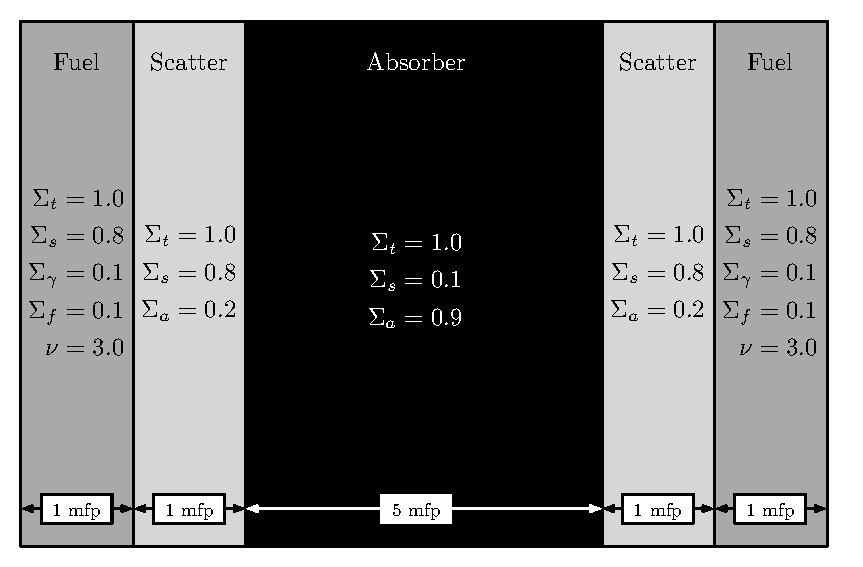
\includegraphics{EntropyandVariance/Data/MultimediaCartoon}
    \caption{Diagram of heterogeneous slab geometry.}
    \label{fig:HeteroGeometry}
\end{figure}

This geometry is particularly difficult for source convergence.  The initial source for this problem lies entirely in the leftmost bin.  With a large highly absorbing slab in the center, it is difficult to move particles from the left to the right side and therefore it will take many histories for the fission source to converge.  The dominance ratio for the symmetric problem is 0.999566 and it is 0.992504 for the asymmetric problem.  For these simulations, 1E5 particles are tracked in each iteration; Arnoldi's method uses 10 iterations per restart and calculated 2 eigenvalues.

The results for the asymmetric problem will be shown first; with a smaller dominance ratio it should be easier to converge the fission source and eigenvalue.  \Fref{fig:AsymmetricPower} shows the convergence of the eigenvalue estimates and fission source as calculated by the power method.  In \Fref{fig:AsymmetricArnoldi} are shown the eigenvalue estimates and fission source convergence for Arnoldi's method.  The solid black line again shows the reference eigenvalue from \citet{Kornreich:2002Semi--0} which is 0.427425.  The dashed line shows the Shannon entropy at the end of the simulation for the power method and the mean of the Shannon entropy for Arnoldi's method.  

The differences in convergence between Arnoldi's method and the power method are easy to see by comparing \Fref{fig:AsymmetricPower} and \Fref{fig:AsymmetricArnoldi}.  We see that Arnoldi's method has converged both the eigenvalue and fission source almost immediately, just like with the homogeneous slab.  The power method however requires 800--900 iterations before the eigenvalue estimates have converged and approximately 1200 iterations before the fission source converges.

\begin{figure}[p]\centering
    \subfloat[Power method.]{\label{fig:AsymmetricPower}% GNUPLOT: LaTeX picture with Postscript
\begingroup%
\makeatletter%
\newcommand{\GNUPLOTspecial}{%
  \@sanitize\catcode`\%=14\relax\special}%
\setlength{\unitlength}{0.0500bp}%
\begin{picture}(8640,5760)(0,0)%
  {\GNUPLOTspecial{"
%!PS-Adobe-2.0 EPSF-2.0
%%Title: AsymmetricPower.tex
%%Creator: gnuplot 4.3 patchlevel 0
%%CreationDate: Sat Aug  1 02:45:15 2009
%%DocumentFonts: 
%%BoundingBox: 0 0 432 288
%%EndComments
%%BeginProlog
/gnudict 256 dict def
gnudict begin
%
% The following true/false flags may be edited by hand if desired.
% The unit line width and grayscale image gamma correction may also be changed.
%
/Color true def
/Blacktext true def
/Solid false def
/Dashlength 1 def
/Landscape false def
/Level1 false def
/Rounded false def
/ClipToBoundingBox false def
/TransparentPatterns false def
/gnulinewidth 5.000 def
/userlinewidth gnulinewidth def
/Gamma 1.0 def
%
/vshift -66 def
/dl1 {
  10.0 Dashlength mul mul
  Rounded { currentlinewidth 0.75 mul sub dup 0 le { pop 0.01 } if } if
} def
/dl2 {
  10.0 Dashlength mul mul
  Rounded { currentlinewidth 0.75 mul add } if
} def
/hpt_ 31.5 def
/vpt_ 31.5 def
/hpt hpt_ def
/vpt vpt_ def
Level1 {} {
/SDict 10 dict def
systemdict /pdfmark known not {
  userdict /pdfmark systemdict /cleartomark get put
} if
SDict begin [
  /Title (AsymmetricPower.tex)
  /Subject (gnuplot plot)
  /Creator (gnuplot 4.3 patchlevel 0)
  /Author (Jeremy Conlin)
%  /Producer (gnuplot)
%  /Keywords ()
  /CreationDate (Sat Aug  1 02:45:15 2009)
  /DOCINFO pdfmark
end
} ifelse
/doclip {
  ClipToBoundingBox {
    newpath 0 0 moveto 432 0 lineto 432 288 lineto 0 288 lineto closepath
    clip
  } if
} def
%
% Gnuplot Prolog Version 4.2 (November 2007)
%
/M {moveto} bind def
/L {lineto} bind def
/R {rmoveto} bind def
/V {rlineto} bind def
/N {newpath moveto} bind def
/Z {closepath} bind def
/C {setrgbcolor} bind def
/f {rlineto fill} bind def
/Gshow {show} def   % May be redefined later in the file to support UTF-8
/vpt2 vpt 2 mul def
/hpt2 hpt 2 mul def
/Lshow {currentpoint stroke M 0 vshift R 
	Blacktext {gsave 0 setgray show grestore} {show} ifelse} def
/Rshow {currentpoint stroke M dup stringwidth pop neg vshift R
	Blacktext {gsave 0 setgray show grestore} {show} ifelse} def
/Cshow {currentpoint stroke M dup stringwidth pop -2 div vshift R 
	Blacktext {gsave 0 setgray show grestore} {show} ifelse} def
/UP {dup vpt_ mul /vpt exch def hpt_ mul /hpt exch def
  /hpt2 hpt 2 mul def /vpt2 vpt 2 mul def} def
/DL {Color {setrgbcolor Solid {pop []} if 0 setdash}
 {pop pop pop 0 setgray Solid {pop []} if 0 setdash} ifelse} def
/BL {stroke userlinewidth 2 mul setlinewidth
	Rounded {1 setlinejoin 1 setlinecap} if} def
/AL {stroke userlinewidth 2 div setlinewidth
	Rounded {1 setlinejoin 1 setlinecap} if} def
/UL {dup gnulinewidth mul /userlinewidth exch def
	dup 1 lt {pop 1} if 10 mul /udl exch def} def
/PL {stroke userlinewidth setlinewidth
	Rounded {1 setlinejoin 1 setlinecap} if} def
% Default Line colors
/LCw {1 1 1} def
/LCb {0 0 0} def
/LCa {0 0 0} def
/LC0 {1 0 0} def
/LC1 {0 1 0} def
/LC2 {0 0 1} def
/LC3 {1 0 1} def
/LC4 {0 1 1} def
/LC5 {1 1 0} def
/LC6 {0 0 0} def
/LC7 {1 0.3 0} def
/LC8 {0.5 0.5 0.5} def
% Default Line Types
/LTw {PL [] 1 setgray} def
/LTb {BL [] LCb DL} def
/LTa {AL [1 udl mul 2 udl mul] 0 setdash LCa setrgbcolor} def
/LT0 {PL [] LC0 DL} def
/LT1 {PL [4 dl1 2 dl2] LC1 DL} def
/LT2 {PL [2 dl1 3 dl2] LC2 DL} def
/LT3 {PL [1 dl1 1.5 dl2] LC3 DL} def
/LT4 {PL [6 dl1 2 dl2 1 dl1 2 dl2] LC4 DL} def
/LT5 {PL [3 dl1 3 dl2 1 dl1 3 dl2] LC5 DL} def
/LT6 {PL [2 dl1 2 dl2 2 dl1 6 dl2] LC6 DL} def
/LT7 {PL [1 dl1 2 dl2 6 dl1 2 dl2 1 dl1 2 dl2] LC7 DL} def
/LT8 {PL [2 dl1 2 dl2 2 dl1 2 dl2 2 dl1 2 dl2 2 dl1 4 dl2] LC8 DL} def
/Pnt {stroke [] 0 setdash gsave 1 setlinecap M 0 0 V stroke grestore} def
/Dia {stroke [] 0 setdash 2 copy vpt add M
  hpt neg vpt neg V hpt vpt neg V
  hpt vpt V hpt neg vpt V closepath stroke
  Pnt} def
/Pls {stroke [] 0 setdash vpt sub M 0 vpt2 V
  currentpoint stroke M
  hpt neg vpt neg R hpt2 0 V stroke
 } def
/Box {stroke [] 0 setdash 2 copy exch hpt sub exch vpt add M
  0 vpt2 neg V hpt2 0 V 0 vpt2 V
  hpt2 neg 0 V closepath stroke
  Pnt} def
/Crs {stroke [] 0 setdash exch hpt sub exch vpt add M
  hpt2 vpt2 neg V currentpoint stroke M
  hpt2 neg 0 R hpt2 vpt2 V stroke} def
/TriU {stroke [] 0 setdash 2 copy vpt 1.12 mul add M
  hpt neg vpt -1.62 mul V
  hpt 2 mul 0 V
  hpt neg vpt 1.62 mul V closepath stroke
  Pnt} def
/Star {2 copy Pls Crs} def
/BoxF {stroke [] 0 setdash exch hpt sub exch vpt add M
  0 vpt2 neg V hpt2 0 V 0 vpt2 V
  hpt2 neg 0 V closepath fill} def
/TriUF {stroke [] 0 setdash vpt 1.12 mul add M
  hpt neg vpt -1.62 mul V
  hpt 2 mul 0 V
  hpt neg vpt 1.62 mul V closepath fill} def
/TriD {stroke [] 0 setdash 2 copy vpt 1.12 mul sub M
  hpt neg vpt 1.62 mul V
  hpt 2 mul 0 V
  hpt neg vpt -1.62 mul V closepath stroke
  Pnt} def
/TriDF {stroke [] 0 setdash vpt 1.12 mul sub M
  hpt neg vpt 1.62 mul V
  hpt 2 mul 0 V
  hpt neg vpt -1.62 mul V closepath fill} def
/DiaF {stroke [] 0 setdash vpt add M
  hpt neg vpt neg V hpt vpt neg V
  hpt vpt V hpt neg vpt V closepath fill} def
/Pent {stroke [] 0 setdash 2 copy gsave
  translate 0 hpt M 4 {72 rotate 0 hpt L} repeat
  closepath stroke grestore Pnt} def
/PentF {stroke [] 0 setdash gsave
  translate 0 hpt M 4 {72 rotate 0 hpt L} repeat
  closepath fill grestore} def
/Circle {stroke [] 0 setdash 2 copy
  hpt 0 360 arc stroke Pnt} def
/CircleF {stroke [] 0 setdash hpt 0 360 arc fill} def
/C0 {BL [] 0 setdash 2 copy moveto vpt 90 450 arc} bind def
/C1 {BL [] 0 setdash 2 copy moveto
	2 copy vpt 0 90 arc closepath fill
	vpt 0 360 arc closepath} bind def
/C2 {BL [] 0 setdash 2 copy moveto
	2 copy vpt 90 180 arc closepath fill
	vpt 0 360 arc closepath} bind def
/C3 {BL [] 0 setdash 2 copy moveto
	2 copy vpt 0 180 arc closepath fill
	vpt 0 360 arc closepath} bind def
/C4 {BL [] 0 setdash 2 copy moveto
	2 copy vpt 180 270 arc closepath fill
	vpt 0 360 arc closepath} bind def
/C5 {BL [] 0 setdash 2 copy moveto
	2 copy vpt 0 90 arc
	2 copy moveto
	2 copy vpt 180 270 arc closepath fill
	vpt 0 360 arc} bind def
/C6 {BL [] 0 setdash 2 copy moveto
	2 copy vpt 90 270 arc closepath fill
	vpt 0 360 arc closepath} bind def
/C7 {BL [] 0 setdash 2 copy moveto
	2 copy vpt 0 270 arc closepath fill
	vpt 0 360 arc closepath} bind def
/C8 {BL [] 0 setdash 2 copy moveto
	2 copy vpt 270 360 arc closepath fill
	vpt 0 360 arc closepath} bind def
/C9 {BL [] 0 setdash 2 copy moveto
	2 copy vpt 270 450 arc closepath fill
	vpt 0 360 arc closepath} bind def
/C10 {BL [] 0 setdash 2 copy 2 copy moveto vpt 270 360 arc closepath fill
	2 copy moveto
	2 copy vpt 90 180 arc closepath fill
	vpt 0 360 arc closepath} bind def
/C11 {BL [] 0 setdash 2 copy moveto
	2 copy vpt 0 180 arc closepath fill
	2 copy moveto
	2 copy vpt 270 360 arc closepath fill
	vpt 0 360 arc closepath} bind def
/C12 {BL [] 0 setdash 2 copy moveto
	2 copy vpt 180 360 arc closepath fill
	vpt 0 360 arc closepath} bind def
/C13 {BL [] 0 setdash 2 copy moveto
	2 copy vpt 0 90 arc closepath fill
	2 copy moveto
	2 copy vpt 180 360 arc closepath fill
	vpt 0 360 arc closepath} bind def
/C14 {BL [] 0 setdash 2 copy moveto
	2 copy vpt 90 360 arc closepath fill
	vpt 0 360 arc} bind def
/C15 {BL [] 0 setdash 2 copy vpt 0 360 arc closepath fill
	vpt 0 360 arc closepath} bind def
/Rec {newpath 4 2 roll moveto 1 index 0 rlineto 0 exch rlineto
	neg 0 rlineto closepath} bind def
/Square {dup Rec} bind def
/Bsquare {vpt sub exch vpt sub exch vpt2 Square} bind def
/S0 {BL [] 0 setdash 2 copy moveto 0 vpt rlineto BL Bsquare} bind def
/S1 {BL [] 0 setdash 2 copy vpt Square fill Bsquare} bind def
/S2 {BL [] 0 setdash 2 copy exch vpt sub exch vpt Square fill Bsquare} bind def
/S3 {BL [] 0 setdash 2 copy exch vpt sub exch vpt2 vpt Rec fill Bsquare} bind def
/S4 {BL [] 0 setdash 2 copy exch vpt sub exch vpt sub vpt Square fill Bsquare} bind def
/S5 {BL [] 0 setdash 2 copy 2 copy vpt Square fill
	exch vpt sub exch vpt sub vpt Square fill Bsquare} bind def
/S6 {BL [] 0 setdash 2 copy exch vpt sub exch vpt sub vpt vpt2 Rec fill Bsquare} bind def
/S7 {BL [] 0 setdash 2 copy exch vpt sub exch vpt sub vpt vpt2 Rec fill
	2 copy vpt Square fill Bsquare} bind def
/S8 {BL [] 0 setdash 2 copy vpt sub vpt Square fill Bsquare} bind def
/S9 {BL [] 0 setdash 2 copy vpt sub vpt vpt2 Rec fill Bsquare} bind def
/S10 {BL [] 0 setdash 2 copy vpt sub vpt Square fill 2 copy exch vpt sub exch vpt Square fill
	Bsquare} bind def
/S11 {BL [] 0 setdash 2 copy vpt sub vpt Square fill 2 copy exch vpt sub exch vpt2 vpt Rec fill
	Bsquare} bind def
/S12 {BL [] 0 setdash 2 copy exch vpt sub exch vpt sub vpt2 vpt Rec fill Bsquare} bind def
/S13 {BL [] 0 setdash 2 copy exch vpt sub exch vpt sub vpt2 vpt Rec fill
	2 copy vpt Square fill Bsquare} bind def
/S14 {BL [] 0 setdash 2 copy exch vpt sub exch vpt sub vpt2 vpt Rec fill
	2 copy exch vpt sub exch vpt Square fill Bsquare} bind def
/S15 {BL [] 0 setdash 2 copy Bsquare fill Bsquare} bind def
/D0 {gsave translate 45 rotate 0 0 S0 stroke grestore} bind def
/D1 {gsave translate 45 rotate 0 0 S1 stroke grestore} bind def
/D2 {gsave translate 45 rotate 0 0 S2 stroke grestore} bind def
/D3 {gsave translate 45 rotate 0 0 S3 stroke grestore} bind def
/D4 {gsave translate 45 rotate 0 0 S4 stroke grestore} bind def
/D5 {gsave translate 45 rotate 0 0 S5 stroke grestore} bind def
/D6 {gsave translate 45 rotate 0 0 S6 stroke grestore} bind def
/D7 {gsave translate 45 rotate 0 0 S7 stroke grestore} bind def
/D8 {gsave translate 45 rotate 0 0 S8 stroke grestore} bind def
/D9 {gsave translate 45 rotate 0 0 S9 stroke grestore} bind def
/D10 {gsave translate 45 rotate 0 0 S10 stroke grestore} bind def
/D11 {gsave translate 45 rotate 0 0 S11 stroke grestore} bind def
/D12 {gsave translate 45 rotate 0 0 S12 stroke grestore} bind def
/D13 {gsave translate 45 rotate 0 0 S13 stroke grestore} bind def
/D14 {gsave translate 45 rotate 0 0 S14 stroke grestore} bind def
/D15 {gsave translate 45 rotate 0 0 S15 stroke grestore} bind def
/DiaE {stroke [] 0 setdash vpt add M
  hpt neg vpt neg V hpt vpt neg V
  hpt vpt V hpt neg vpt V closepath stroke} def
/BoxE {stroke [] 0 setdash exch hpt sub exch vpt add M
  0 vpt2 neg V hpt2 0 V 0 vpt2 V
  hpt2 neg 0 V closepath stroke} def
/TriUE {stroke [] 0 setdash vpt 1.12 mul add M
  hpt neg vpt -1.62 mul V
  hpt 2 mul 0 V
  hpt neg vpt 1.62 mul V closepath stroke} def
/TriDE {stroke [] 0 setdash vpt 1.12 mul sub M
  hpt neg vpt 1.62 mul V
  hpt 2 mul 0 V
  hpt neg vpt -1.62 mul V closepath stroke} def
/PentE {stroke [] 0 setdash gsave
  translate 0 hpt M 4 {72 rotate 0 hpt L} repeat
  closepath stroke grestore} def
/CircE {stroke [] 0 setdash 
  hpt 0 360 arc stroke} def
/Opaque {gsave closepath 1 setgray fill grestore 0 setgray closepath} def
/DiaW {stroke [] 0 setdash vpt add M
  hpt neg vpt neg V hpt vpt neg V
  hpt vpt V hpt neg vpt V Opaque stroke} def
/BoxW {stroke [] 0 setdash exch hpt sub exch vpt add M
  0 vpt2 neg V hpt2 0 V 0 vpt2 V
  hpt2 neg 0 V Opaque stroke} def
/TriUW {stroke [] 0 setdash vpt 1.12 mul add M
  hpt neg vpt -1.62 mul V
  hpt 2 mul 0 V
  hpt neg vpt 1.62 mul V Opaque stroke} def
/TriDW {stroke [] 0 setdash vpt 1.12 mul sub M
  hpt neg vpt 1.62 mul V
  hpt 2 mul 0 V
  hpt neg vpt -1.62 mul V Opaque stroke} def
/PentW {stroke [] 0 setdash gsave
  translate 0 hpt M 4 {72 rotate 0 hpt L} repeat
  Opaque stroke grestore} def
/CircW {stroke [] 0 setdash 
  hpt 0 360 arc Opaque stroke} def
/BoxFill {gsave Rec 1 setgray fill grestore} def
/Density {
  /Fillden exch def
  currentrgbcolor
  /ColB exch def /ColG exch def /ColR exch def
  /ColR ColR Fillden mul Fillden sub 1 add def
  /ColG ColG Fillden mul Fillden sub 1 add def
  /ColB ColB Fillden mul Fillden sub 1 add def
  ColR ColG ColB setrgbcolor} def
/BoxColFill {gsave Rec PolyFill} def
/PolyFill {gsave Density fill grestore grestore} def
/h {rlineto rlineto rlineto gsave closepath fill grestore} bind def
%
% PostScript Level 1 Pattern Fill routine for rectangles
% Usage: x y w h s a XX PatternFill
%	x,y = lower left corner of box to be filled
%	w,h = width and height of box
%	  a = angle in degrees between lines and x-axis
%	 XX = 0/1 for no/yes cross-hatch
%
/PatternFill {gsave /PFa [ 9 2 roll ] def
  PFa 0 get PFa 2 get 2 div add PFa 1 get PFa 3 get 2 div add translate
  PFa 2 get -2 div PFa 3 get -2 div PFa 2 get PFa 3 get Rec
  gsave 1 setgray fill grestore clip
  currentlinewidth 0.5 mul setlinewidth
  /PFs PFa 2 get dup mul PFa 3 get dup mul add sqrt def
  0 0 M PFa 5 get rotate PFs -2 div dup translate
  0 1 PFs PFa 4 get div 1 add floor cvi
	{PFa 4 get mul 0 M 0 PFs V} for
  0 PFa 6 get ne {
	0 1 PFs PFa 4 get div 1 add floor cvi
	{PFa 4 get mul 0 2 1 roll M PFs 0 V} for
 } if
  stroke grestore} def
%
/languagelevel where
 {pop languagelevel} {1} ifelse
 2 lt
	{/InterpretLevel1 true def}
	{/InterpretLevel1 Level1 def}
 ifelse
%
% PostScript level 2 pattern fill definitions
%
/Level2PatternFill {
/Tile8x8 {/PaintType 2 /PatternType 1 /TilingType 1 /BBox [0 0 8 8] /XStep 8 /YStep 8}
	bind def
/KeepColor {currentrgbcolor [/Pattern /DeviceRGB] setcolorspace} bind def
<< Tile8x8
 /PaintProc {0.5 setlinewidth pop 0 0 M 8 8 L 0 8 M 8 0 L stroke} 
>> matrix makepattern
/Pat1 exch def
<< Tile8x8
 /PaintProc {0.5 setlinewidth pop 0 0 M 8 8 L 0 8 M 8 0 L stroke
	0 4 M 4 8 L 8 4 L 4 0 L 0 4 L stroke}
>> matrix makepattern
/Pat2 exch def
<< Tile8x8
 /PaintProc {0.5 setlinewidth pop 0 0 M 0 8 L
	8 8 L 8 0 L 0 0 L fill}
>> matrix makepattern
/Pat3 exch def
<< Tile8x8
 /PaintProc {0.5 setlinewidth pop -4 8 M 8 -4 L
	0 12 M 12 0 L stroke}
>> matrix makepattern
/Pat4 exch def
<< Tile8x8
 /PaintProc {0.5 setlinewidth pop -4 0 M 8 12 L
	0 -4 M 12 8 L stroke}
>> matrix makepattern
/Pat5 exch def
<< Tile8x8
 /PaintProc {0.5 setlinewidth pop -2 8 M 4 -4 L
	0 12 M 8 -4 L 4 12 M 10 0 L stroke}
>> matrix makepattern
/Pat6 exch def
<< Tile8x8
 /PaintProc {0.5 setlinewidth pop -2 0 M 4 12 L
	0 -4 M 8 12 L 4 -4 M 10 8 L stroke}
>> matrix makepattern
/Pat7 exch def
<< Tile8x8
 /PaintProc {0.5 setlinewidth pop 8 -2 M -4 4 L
	12 0 M -4 8 L 12 4 M 0 10 L stroke}
>> matrix makepattern
/Pat8 exch def
<< Tile8x8
 /PaintProc {0.5 setlinewidth pop 0 -2 M 12 4 L
	-4 0 M 12 8 L -4 4 M 8 10 L stroke}
>> matrix makepattern
/Pat9 exch def
/Pattern1 {PatternBgnd KeepColor Pat1 setpattern} bind def
/Pattern2 {PatternBgnd KeepColor Pat2 setpattern} bind def
/Pattern3 {PatternBgnd KeepColor Pat3 setpattern} bind def
/Pattern4 {PatternBgnd KeepColor Landscape {Pat5} {Pat4} ifelse setpattern} bind def
/Pattern5 {PatternBgnd KeepColor Landscape {Pat4} {Pat5} ifelse setpattern} bind def
/Pattern6 {PatternBgnd KeepColor Landscape {Pat9} {Pat6} ifelse setpattern} bind def
/Pattern7 {PatternBgnd KeepColor Landscape {Pat8} {Pat7} ifelse setpattern} bind def
} def
%
%
%End of PostScript Level 2 code
%
/PatternBgnd {
  TransparentPatterns {} {gsave 1 setgray fill grestore} ifelse
} def
%
% Substitute for Level 2 pattern fill codes with
% grayscale if Level 2 support is not selected.
%
/Level1PatternFill {
/Pattern1 {0.250 Density} bind def
/Pattern2 {0.500 Density} bind def
/Pattern3 {0.750 Density} bind def
/Pattern4 {0.125 Density} bind def
/Pattern5 {0.375 Density} bind def
/Pattern6 {0.625 Density} bind def
/Pattern7 {0.875 Density} bind def
} def
%
% Now test for support of Level 2 code
%
Level1 {Level1PatternFill} {Level2PatternFill} ifelse
%
/Symbol-Oblique /Symbol findfont [1 0 .167 1 0 0] makefont
dup length dict begin {1 index /FID eq {pop pop} {def} ifelse} forall
currentdict end definefont pop
end
%%EndProlog
gnudict begin
gsave
doclip
0 0 translate
0.050 0.050 scale
0 setgray
newpath
1.000 UL
LTb
1340 640 M
63 0 V
-63 813 R
63 0 V
-63 813 R
63 0 V
-63 814 R
63 0 V
-63 813 R
63 0 V
-63 813 R
63 0 V
-63 813 R
63 0 V
1340 640 M
0 63 V
0 4816 R
0 -63 V
1948 640 M
0 63 V
0 4816 R
0 -63 V
2556 640 M
0 63 V
0 4816 R
0 -63 V
3164 640 M
0 63 V
0 4816 R
0 -63 V
3772 640 M
0 63 V
0 4816 R
0 -63 V
4380 640 M
0 63 V
0 4816 R
0 -63 V
4987 640 M
0 63 V
0 4816 R
0 -63 V
5595 640 M
0 63 V
0 4816 R
0 -63 V
6203 640 M
0 63 V
0 4816 R
0 -63 V
6811 640 M
0 63 V
0 4816 R
0 -63 V
7419 640 M
0 63 V
0 4816 R
0 -63 V
0 -4816 R
-63 0 V
63 542 R
-63 0 V
63 542 R
-63 0 V
63 542 R
-63 0 V
63 542 R
-63 0 V
63 543 R
-63 0 V
63 542 R
-63 0 V
63 542 R
-63 0 V
63 542 R
-63 0 V
63 542 R
-63 0 V
stroke
1340 5519 N
0 -4879 V
6079 0 V
0 4879 V
-6079 0 V
Z stroke
LCb setrgbcolor
LTb
LCb setrgbcolor
LTb
LCb setrgbcolor
LTb
LCb setrgbcolor
LTb
1.000 UP
1.000 UL
LTb
1.000 UL
LTb
5316 703 N
0 600 V
1983 0 V
0 -600 V
-1983 0 V
Z stroke
5316 1303 M
1983 0 V
stroke
LT0
LCb setrgbcolor
LT0
6636 1103 M
543 0 V
1342 640 M
3 3116 V
2 678 V
3 139 V
2 -58 V
3 -171 V
2 474 V
2 -313 V
3 131 V
2 -18 V
3 83 V
2 -31 V
3 -48 V
2 19 V
2 65 V
3 -31 V
2 -16 V
3 -164 V
2 98 V
3 51 V
2 50 V
2 -7 V
3 -43 V
2 -31 V
3 -102 V
2 65 V
3 121 V
2 -290 V
3 47 V
2 138 V
2 52 V
3 9 V
2 3 V
3 -175 V
2 22 V
3 125 V
2 8 V
2 17 V
3 -215 V
2 243 V
3 124 V
2 -296 V
3 153 V
2 29 V
2 -30 V
3 -78 V
2 67 V
3 -209 V
2 38 V
3 221 V
2 22 V
2 -89 V
3 -173 V
2 236 V
3 -20 V
2 -276 V
3 191 V
2 17 V
2 11 V
3 -121 V
2 64 V
3 181 V
2 -106 V
3 15 V
2 -136 V
2 -28 V
3 185 V
2 -231 V
3 184 V
2 49 V
3 -272 V
2 12 V
3 161 V
2 11 V
2 6 V
3 17 V
2 -100 V
3 120 V
2 -63 V
3 20 V
2 146 V
2 -128 V
3 -11 V
2 22 V
3 -127 V
2 336 V
3 -213 V
2 -7 V
2 -41 V
3 100 V
2 -217 V
3 257 V
2 -146 V
3 -70 V
2 226 V
2 -65 V
3 126 V
2 -217 V
3 219 V
2 -14 V
3 -123 V
2 -236 V
2 198 V
stroke 1590 4602 M
3 -32 V
2 133 V
3 -73 V
2 -54 V
3 -1 V
2 15 V
2 -28 V
3 117 V
2 25 V
3 -41 V
2 -95 V
3 137 V
2 11 V
2 -35 V
3 17 V
2 -52 V
3 137 V
2 -6 V
3 -56 V
2 -59 V
3 110 V
2 -98 V
2 5 V
3 -35 V
2 75 V
3 -266 V
2 157 V
3 6 V
2 -49 V
2 -70 V
3 24 V
2 182 V
3 -259 V
2 96 V
3 60 V
2 23 V
2 -74 V
3 194 V
2 -96 V
3 46 V
2 -196 V
3 141 V
2 -240 V
2 170 V
3 193 V
2 -54 V
3 -130 V
2 -21 V
3 239 V
2 -186 V
2 -10 V
3 87 V
2 14 V
3 -198 V
2 129 V
3 -12 V
2 115 V
2 -49 V
3 -123 V
2 21 V
3 -47 V
2 82 V
3 -69 V
2 27 V
3 47 V
2 0 V
2 169 V
3 -83 V
2 9 V
3 -212 V
2 8 V
3 78 V
2 49 V
2 -134 V
3 268 V
2 -80 V
3 -152 V
2 150 V
3 -235 V
2 356 V
2 -51 V
3 -197 V
2 57 V
3 -78 V
2 214 V
3 -320 V
2 184 V
2 108 V
3 -237 V
2 170 V
3 22 V
2 -56 V
3 68 V
2 26 V
2 -86 V
3 -13 V
2 -126 V
3 102 V
2 101 V
3 42 V
2 -234 V
2 356 V
3 -268 V
2 116 V
stroke 1843 4714 M
3 -93 V
2 -91 V
3 159 V
2 66 V
2 -184 V
3 139 V
2 -204 V
3 218 V
2 67 V
3 -204 V
2 47 V
3 -58 V
2 14 V
2 68 V
3 78 V
2 -83 V
3 -3 V
2 -53 V
3 43 V
2 34 V
2 -9 V
3 -48 V
2 -33 V
3 -9 V
2 205 V
3 -195 V
2 22 V
2 -78 V
3 173 V
2 63 V
3 35 V
2 -287 V
3 63 V
2 38 V
2 46 V
3 -61 V
2 -59 V
3 53 V
2 11 V
3 82 V
2 23 V
2 -28 V
3 53 V
2 -24 V
3 -74 V
2 24 V
3 0 V
2 -1 V
2 -117 V
3 152 V
2 -79 V
3 138 V
2 -181 V
3 128 V
2 -90 V
3 51 V
2 -113 V
2 127 V
3 68 V
2 85 V
3 -134 V
2 57 V
3 -154 V
2 121 V
2 -47 V
3 -37 V
2 133 V
3 -11 V
2 -64 V
3 -75 V
2 1 V
2 140 V
3 15 V
2 -65 V
3 -102 V
2 265 V
3 -307 V
2 171 V
2 51 V
3 -91 V
2 -15 V
3 -74 V
2 120 V
3 8 V
2 -89 V
2 194 V
3 23 V
2 -126 V
3 27 V
2 -136 V
3 126 V
2 -60 V
2 -162 V
3 83 V
2 105 V
3 -265 V
2 234 V
3 5 V
2 -26 V
3 101 V
2 -81 V
2 -108 V
3 12 V
2 -69 V
stroke 2096 4522 M
3 346 V
2 -200 V
3 85 V
2 -33 V
2 79 V
3 -101 V
2 -112 V
3 150 V
2 59 V
3 -158 V
2 -32 V
2 204 V
3 -35 V
2 12 V
3 -143 V
2 -29 V
3 193 V
2 -68 V
2 63 V
3 -116 V
2 -98 V
3 32 V
2 220 V
3 -120 V
2 43 V
2 81 V
3 -78 V
2 23 V
3 -55 V
2 36 V
3 15 V
2 -27 V
2 -3 V
3 -158 V
2 191 V
3 -36 V
2 -59 V
3 -38 V
2 39 V
2 -29 V
3 11 V
2 31 V
3 78 V
2 -87 V
3 -7 V
2 108 V
3 -55 V
2 13 V
2 11 V
3 -49 V
2 106 V
3 -140 V
2 -60 V
3 144 V
2 -18 V
2 58 V
3 21 V
2 -158 V
3 123 V
2 7 V
3 -150 V
2 142 V
2 -78 V
3 83 V
2 -89 V
3 31 V
2 -124 V
3 173 V
2 -110 V
2 17 V
3 -37 V
2 103 V
3 6 V
2 34 V
3 18 V
2 -34 V
2 -99 V
3 50 V
2 44 V
3 -33 V
2 28 V
3 54 V
2 70 V
2 -67 V
3 -227 V
2 210 V
3 8 V
2 -8 V
3 -18 V
2 -175 V
3 161 V
2 118 V
2 -81 V
3 26 V
2 -205 V
3 77 V
2 -69 V
3 61 V
2 116 V
2 -21 V
3 -97 V
2 88 V
3 -32 V
2 31 V
stroke 2349 4797 M
3 -134 V
2 203 V
2 -152 V
3 72 V
2 -28 V
3 99 V
2 -99 V
3 142 V
2 -148 V
2 -23 V
3 -95 V
2 193 V
3 -126 V
2 110 V
3 19 V
2 -99 V
2 75 V
3 -35 V
2 -77 V
3 149 V
2 -4 V
3 -246 V
2 255 V
2 -194 V
3 123 V
2 102 V
3 -92 V
2 47 V
3 -38 V
2 -43 V
2 -162 V
3 88 V
2 184 V
3 -140 V
2 93 V
3 19 V
2 28 V
3 7 V
2 -187 V
2 254 V
3 -135 V
2 -91 V
3 146 V
2 -82 V
3 71 V
2 -84 V
2 125 V
3 -108 V
2 -189 V
3 222 V
2 10 V
3 -148 V
2 49 V
2 149 V
3 -81 V
2 158 V
3 -217 V
2 146 V
3 -158 V
2 196 V
2 -123 V
3 -77 V
2 -81 V
3 267 V
2 -138 V
3 -18 V
2 143 V
2 -78 V
3 43 V
2 -53 V
3 125 V
2 -170 V
3 77 V
2 -94 V
2 71 V
3 -71 V
2 308 V
3 -261 V
2 24 V
3 -17 V
2 73 V
3 90 V
2 -80 V
2 -177 V
3 152 V
2 -97 V
3 111 V
2 49 V
3 -132 V
2 125 V
2 31 V
3 -81 V
2 -57 V
3 150 V
2 -5 V
3 -91 V
2 -54 V
2 -192 V
3 318 V
2 -56 V
3 -97 V
2 212 V
3 -114 V
2 -111 V
stroke 2602 4760 M
2 44 V
3 -33 V
2 147 V
3 10 V
2 -49 V
3 83 V
2 -143 V
2 88 V
3 -31 V
2 58 V
3 10 V
2 -174 V
3 83 V
2 34 V
2 -161 V
3 81 V
2 20 V
3 -132 V
2 141 V
3 39 V
2 73 V
2 -121 V
3 90 V
2 66 V
3 14 V
2 -86 V
3 150 V
2 -22 V
3 -125 V
2 70 V
2 -20 V
3 -68 V
2 21 V
3 -6 V
2 -98 V
3 183 V
2 -62 V
2 -47 V
3 143 V
2 3 V
3 -144 V
2 -180 V
3 323 V
2 -31 V
2 -97 V
3 9 V
2 -11 V
3 19 V
2 -61 V
3 28 V
2 -1 V
2 -28 V
3 -5 V
2 82 V
3 39 V
2 32 V
3 38 V
2 -5 V
2 -145 V
3 -187 V
2 281 V
3 -8 V
2 -10 V
3 -17 V
2 73 V
2 -301 V
3 218 V
2 115 V
3 -70 V
2 -52 V
3 33 V
2 19 V
3 -75 V
2 85 V
2 -245 V
3 144 V
2 160 V
3 -117 V
2 -30 V
3 -90 V
2 -19 V
2 230 V
3 -249 V
2 53 V
3 207 V
2 34 V
3 -188 V
2 97 V
2 135 V
3 -269 V
2 184 V
3 -155 V
2 51 V
3 17 V
2 -27 V
2 59 V
3 188 V
2 -378 V
3 50 V
2 -23 V
3 83 V
2 139 V
2 71 V
3 -134 V
stroke 2855 4977 M
2 121 V
3 -258 V
2 213 V
3 46 V
2 5 V
2 -196 V
3 -104 V
2 252 V
3 -255 V
2 55 V
3 307 V
2 -173 V
2 -3 V
3 88 V
2 -86 V
3 -4 V
2 123 V
3 -60 V
2 -34 V
3 -46 V
2 126 V
2 7 V
3 -138 V
2 87 V
3 -32 V
2 -278 V
3 232 V
2 -157 V
2 357 V
3 -43 V
2 -161 V
3 100 V
2 -259 V
3 175 V
2 194 V
2 -323 V
3 39 V
2 -9 V
3 306 V
2 -153 V
3 -8 V
2 -56 V
2 -114 V
3 288 V
2 -224 V
3 64 V
2 -3 V
3 -97 V
2 39 V
2 61 V
3 -4 V
2 134 V
3 -189 V
2 88 V
3 -91 V
2 56 V
2 137 V
3 -79 V
2 86 V
3 -69 V
2 -106 V
3 100 V
2 115 V
3 -93 V
2 -59 V
2 -33 V
3 -26 V
2 184 V
3 -212 V
2 -27 V
3 133 V
2 223 V
2 -335 V
3 292 V
2 -67 V
3 -183 V
2 37 V
3 -63 V
2 176 V
2 -228 V
3 186 V
2 -250 V
3 306 V
2 -129 V
3 -40 V
2 -9 V
2 -9 V
3 21 V
2 56 V
3 -18 V
2 -113 V
3 108 V
2 -162 V
2 195 V
3 264 V
2 -318 V
3 28 V
2 36 V
3 -112 V
2 11 V
2 93 V
3 167 V
2 -110 V
3 -100 V
stroke 3108 4986 M
2 38 V
3 -2 V
2 -37 V
2 9 V
3 -29 V
2 177 V
3 -88 V
2 36 V
3 -74 V
2 -148 V
3 97 V
2 143 V
2 -151 V
3 147 V
2 -179 V
3 69 V
2 245 V
3 -115 V
2 -157 V
2 38 V
3 -115 V
2 45 V
3 109 V
2 89 V
3 -221 V
2 123 V
2 -197 V
3 11 V
2 223 V
3 -243 V
2 133 V
3 -11 V
2 71 V
2 -62 V
3 -107 V
2 192 V
3 -45 V
2 32 V
3 37 V
2 -129 V
2 78 V
3 210 V
2 -153 V
3 -75 V
2 -32 V
3 332 V
2 -210 V
2 -60 V
3 120 V
2 -60 V
3 88 V
2 -123 V
3 57 V
2 -108 V
3 237 V
2 -97 V
2 -23 V
3 106 V
2 -131 V
3 -4 V
2 22 V
3 2 V
2 -67 V
2 64 V
3 59 V
2 -194 V
3 55 V
2 -108 V
3 100 V
2 -4 V
2 23 V
3 70 V
2 -74 V
3 15 V
2 -117 V
3 -27 V
2 153 V
2 -36 V
3 194 V
2 -181 V
3 -100 V
2 230 V
3 -143 V
2 -88 V
2 -13 V
3 142 V
2 30 V
3 -29 V
2 -189 V
3 33 V
2 230 V
2 61 V
3 -134 V
2 16 V
3 -31 V
2 -44 V
3 36 V
2 -87 V
3 33 V
2 91 V
2 139 V
3 -190 V
2 9 V
3 3 V
stroke 3361 5046 M
2 42 V
3 121 V
2 -105 V
2 -117 V
3 8 V
2 161 V
3 -138 V
2 101 V
3 -58 V
2 5 V
2 57 V
3 -127 V
2 150 V
3 -64 V
2 -137 V
3 -62 V
2 212 V
2 50 V
3 -100 V
2 156 V
3 -37 V
2 97 V
3 -186 V
2 -100 V
2 -46 V
3 48 V
2 143 V
3 -79 V
2 -12 V
3 -81 V
2 145 V
2 81 V
3 -141 V
2 81 V
3 -4 V
2 106 V
3 -119 V
2 -12 V
2 -88 V
3 108 V
2 -29 V
3 -96 V
2 156 V
3 66 V
2 -40 V
3 -117 V
2 29 V
2 7 V
3 -88 V
2 6 V
3 15 V
2 80 V
3 -56 V
2 -16 V
2 2 V
3 -42 V
2 13 V
3 101 V
2 -42 V
3 -146 V
2 211 V
2 32 V
3 -281 V
2 128 V
3 234 V
2 -321 V
3 166 V
2 66 V
2 -175 V
3 213 V
2 -5 V
3 -53 V
2 -50 V
3 -14 V
2 72 V
2 -143 V
3 103 V
2 -86 V
3 52 V
2 137 V
3 -83 V
2 -37 V
2 220 V
3 -84 V
2 -15 V
3 -161 V
2 5 V
3 3 V
2 -40 V
3 194 V
2 -11 V
2 -52 V
3 -76 V
2 228 V
3 -93 V
2 -85 V
3 -62 V
2 -22 V
2 153 V
3 -178 V
2 197 V
3 -184 V
2 84 V
3 59 V
stroke 3614 5154 M
2 26 V
2 -161 V
3 -29 V
2 96 V
3 57 V
2 -110 V
3 -189 V
2 220 V
2 48 V
3 -111 V
2 61 V
3 27 V
2 55 V
3 -30 V
2 -44 V
2 138 V
3 21 V
2 -190 V
3 114 V
2 114 V
3 -189 V
2 -72 V
2 246 V
3 -85 V
2 38 V
3 -128 V
2 142 V
3 -76 V
2 42 V
2 -157 V
3 153 V
2 -88 V
3 -173 V
2 85 V
3 84 V
2 -28 V
3 263 V
2 -120 V
2 -98 V
3 -85 V
2 327 V
3 -195 V
2 -119 V
3 168 V
2 80 V
2 -232 V
3 -33 V
2 -97 V
3 87 V
2 144 V
3 -124 V
2 83 V
2 136 V
3 -164 V
2 -115 V
3 -44 V
2 249 V
3 -83 V
2 58 V
2 -127 V
3 147 V
2 -28 V
3 156 V
2 -244 V
3 -30 V
2 13 V
2 48 V
3 8 V
2 -31 V
3 -38 V
2 129 V
3 -67 V
2 -85 V
2 97 V
3 -11 V
2 -57 V
3 -8 V
2 195 V
3 -100 V
2 -130 V
3 8 V
2 22 V
2 224 V
3 -177 V
2 56 V
3 -34 V
2 38 V
3 -95 V
2 202 V
2 -71 V
3 -8 V
2 -95 V
3 5 V
2 44 V
3 14 V
2 61 V
2 81 V
3 -236 V
2 181 V
3 -89 V
2 122 V
3 -256 V
2 275 V
2 -70 V
stroke 3866 5186 M
3 -147 V
2 96 V
3 55 V
2 -55 V
3 -28 V
2 -78 V
2 -18 V
3 158 V
2 -61 V
3 -14 V
2 -11 V
3 32 V
2 51 V
2 -42 V
3 -25 V
2 61 V
3 -226 V
2 167 V
3 113 V
2 -152 V
2 -173 V
3 186 V
2 81 V
3 -44 V
2 -44 V
3 188 V
2 -397 V
3 357 V
2 -79 V
2 -99 V
3 -16 V
2 -5 V
3 -8 V
2 94 V
3 -53 V
2 204 V
2 -158 V
3 -77 V
2 91 V
3 -61 V
2 102 V
3 92 V
2 1 V
2 -153 V
3 95 V
2 -108 V
3 31 V
2 245 V
3 -195 V
2 -169 V
2 154 V
3 15 V
2 60 V
3 -65 V
2 -34 V
3 -94 V
2 49 V
2 33 V
3 -142 V
2 151 V
3 -100 V
2 117 V
3 -74 V
2 -129 V
2 103 V
3 113 V
2 -99 V
3 -35 V
2 139 V
3 -240 V
2 163 V
3 121 V
2 -128 V
2 61 V
3 3 V
2 36 V
3 -68 V
2 -166 V
3 159 V
2 73 V
2 40 V
3 -80 V
2 -29 V
3 -62 V
2 117 V
3 -49 V
2 9 V
2 -138 V
3 5 V
2 149 V
3 -102 V
2 113 V
3 -24 V
2 41 V
2 -116 V
3 -50 V
2 37 V
3 45 V
2 -27 V
3 88 V
2 92 V
2 -58 V
3 -142 V
2 115 V
stroke 4119 5140 M
3 -5 V
2 36 V
3 -16 V
2 -5 V
2 70 V
3 75 V
2 -289 V
3 287 V
2 -247 V
3 49 V
2 -34 V
2 8 V
3 -102 V
2 169 V
3 -14 V
2 -121 V
3 20 V
2 29 V
3 128 V
2 -147 V
2 70 V
3 -59 V
2 30 V
3 -64 V
2 18 V
3 125 V
2 -128 V
2 73 V
3 -94 V
2 48 V
3 85 V
2 123 V
3 -145 V
2 -127 V
2 254 V
3 -48 V
2 -272 V
3 97 V
2 5 V
3 159 V
2 -113 V
2 -15 V
3 18 V
2 113 V
3 -36 V
2 -110 V
3 222 V
2 -131 V
2 -13 V
3 7 V
2 15 V
3 -81 V
2 112 V
3 -154 V
2 -51 V
2 113 V
3 -83 V
2 246 V
3 -150 V
2 26 V
3 -80 V
2 189 V
3 -245 V
2 68 V
2 -100 V
3 280 V
2 -33 V
3 -63 V
2 -39 V
3 -34 V
2 -95 V
2 189 V
3 161 V
2 -97 V
3 -74 V
2 -122 V
3 195 V
2 -103 V
2 19 V
3 -100 V
2 35 V
3 139 V
2 -11 V
3 -70 V
2 -162 V
2 182 V
3 -111 V
2 106 V
3 -77 V
2 -59 V
3 126 V
2 -1 V
2 196 V
3 -223 V
2 -156 V
3 188 V
2 -203 V
3 234 V
2 -12 V
2 -27 V
3 -172 V
2 176 V
3 7 V
2 -84 V
stroke 4372 5053 M
3 45 V
2 -33 V
3 -87 V
2 175 V
2 -40 V
3 -41 V
2 -41 V
3 -39 V
2 122 V
3 32 V
2 -97 V
2 -12 V
3 -3 V
2 -28 V
3 43 V
2 -2 V
3 -24 V
2 -24 V
2 -37 V
3 113 V
2 -90 V
3 243 V
2 -172 V
3 73 V
2 118 V
2 -126 V
3 -96 V
2 -52 V
3 112 V
2 19 V
3 51 V
2 -177 V
2 307 V
3 -160 V
2 48 V
3 46 V
2 -35 V
3 104 V
2 -324 V
2 239 V
3 -190 V
2 51 V
3 105 V
2 -243 V
3 229 V
2 -52 V
2 -10 V
3 -152 V
2 168 V
3 34 V
2 -113 V
3 204 V
2 -232 V
3 65 V
2 -59 V
2 231 V
3 -174 V
2 25 V
3 42 V
2 98 V
3 -74 V
2 -86 V
2 171 V
3 13 V
2 -95 V
3 -40 V
2 -125 V
3 125 V
2 30 V
2 36 V
3 -231 V
2 24 V
3 83 V
2 60 V
3 91 V
2 -242 V
2 89 V
3 -44 V
2 -90 V
3 315 V
2 -33 V
3 0 V
2 -254 V
2 96 V
3 114 V
2 3 V
3 -40 V
2 -103 V
3 -22 V
2 236 V
2 -119 V
3 -21 V
2 62 V
3 -53 V
2 -7 V
3 93 V
2 -121 V
3 -44 V
2 102 V
2 79 V
3 -146 V
2 45 V
3 147 V
2 -227 V
stroke 4625 5027 M
3 -10 V
2 47 V
2 -94 V
3 164 V
2 -81 V
3 17 V
2 -51 V
3 39 V
2 -20 V
2 -26 V
3 119 V
2 68 V
3 49 V
2 -191 V
3 155 V
2 -118 V
2 70 V
3 -99 V
2 -34 V
3 254 V
2 -252 V
3 133 V
2 -113 V
2 149 V
3 120 V
2 -260 V
3 -46 V
2 -4 V
3 177 V
2 31 V
2 -27 V
3 -14 V
2 -112 V
3 31 V
2 8 V
3 -71 V
2 189 V
2 -95 V
3 -13 V
2 107 V
3 -86 V
2 -41 V
3 -54 V
2 178 V
3 -187 V
2 80 V
2 -58 V
3 -83 V
2 156 V
3 -41 V
2 97 V
3 -325 V
2 290 V
2 -27 V
3 -138 V
2 127 V
3 48 V
2 -19 V
3 -166 V
2 14 V
2 213 V
3 -70 V
2 -132 V
3 116 V
2 -46 V
3 14 V
2 169 V
2 -254 V
3 42 V
2 10 V
3 -74 V
2 16 V
3 57 V
2 -111 V
2 80 V
3 51 V
2 -50 V
3 -5 V
2 117 V
3 -173 V
2 195 V
2 -144 V
3 14 V
2 214 V
3 -137 V
2 -39 V
3 -16 V
2 -109 V
3 39 V
2 178 V
2 -20 V
3 20 V
2 -52 V
3 23 V
2 37 V
3 -173 V
2 -48 V
2 137 V
3 143 V
2 -97 V
3 -10 V
2 -55 V
3 98 V
2 -173 V
stroke 4878 4983 M
2 145 V
3 -80 V
2 50 V
3 94 V
2 -89 V
3 75 V
2 -132 V
2 68 V
3 -28 V
2 1 V
3 -36 V
2 146 V
3 -156 V
2 104 V
2 12 V
3 -77 V
2 133 V
3 -91 V
2 0 V
3 3 V
2 225 V
2 -137 V
3 -122 V
2 -49 V
3 -16 V
2 -33 V
3 166 V
2 -167 V
2 180 V
3 -91 V
2 86 V
3 -53 V
2 127 V
3 -154 V
2 49 V
3 5 V
2 -149 V
2 194 V
3 -28 V
2 -74 V
3 -46 V
2 213 V
3 -166 V
2 150 V
2 -233 V
3 52 V
2 -8 V
3 48 V
2 11 V
3 -84 V
2 137 V
2 -157 V
3 157 V
2 -36 V
3 26 V
2 -108 V
3 96 V
2 -14 V
2 46 V
3 -99 V
2 174 V
3 239 V
2 -425 V
3 -88 V
2 38 V
2 -77 V
3 122 V
2 42 V
3 -29 V
2 209 V
3 -136 V
2 -145 V
2 51 V
3 6 V
2 154 V
3 -138 V
2 -38 V
3 40 V
2 20 V
3 171 V
2 -47 V
2 26 V
3 -346 V
2 174 V
3 88 V
2 -47 V
3 97 V
2 -172 V
2 48 V
3 158 V
2 -112 V
3 23 V
2 -45 V
3 129 V
2 -115 V
2 -6 V
3 93 V
2 -20 V
3 -3 V
2 -182 V
3 139 V
2 -70 V
2 123 V
3 -166 V
stroke 5131 5026 M
2 91 V
3 -170 V
2 145 V
3 -70 V
2 -7 V
2 287 V
3 -213 V
2 51 V
3 -74 V
2 -123 V
3 24 V
2 118 V
2 -19 V
3 81 V
2 56 V
3 -317 V
2 334 V
3 -50 V
2 79 V
2 -162 V
3 -45 V
2 113 V
3 35 V
2 -90 V
3 -114 V
2 94 V
3 132 V
2 -305 V
2 98 V
3 -16 V
2 153 V
3 -107 V
2 114 V
3 15 V
2 -217 V
2 172 V
3 100 V
2 -92 V
3 31 V
2 -91 V
3 131 V
2 -129 V
2 200 V
3 -174 V
2 59 V
3 -11 V
2 -85 V
3 128 V
2 -198 V
2 -55 V
3 141 V
2 -88 V
3 57 V
2 -94 V
3 88 V
2 -13 V
2 39 V
3 187 V
2 -145 V
3 -122 V
2 -92 V
3 218 V
2 29 V
2 -76 V
3 56 V
2 -21 V
3 25 V
2 52 V
3 -119 V
2 74 V
3 231 V
2 -401 V
2 262 V
3 27 V
2 -181 V
3 82 V
2 9 V
3 -56 V
2 -140 V
2 147 V
3 -22 V
2 82 V
3 -38 V
2 -31 V
3 -39 V
2 195 V
2 -277 V
3 106 V
2 101 V
3 -32 V
2 -93 V
3 -41 V
2 34 V
2 71 V
3 78 V
2 -62 V
3 -119 V
2 -24 V
3 203 V
2 -170 V
2 35 V
3 -35 V
2 49 V
3 -111 V
stroke 5384 4969 M
2 104 V
3 83 V
2 -141 V
2 107 V
3 -66 V
2 16 V
3 -66 V
2 76 V
3 -71 V
2 20 V
2 0 V
3 89 V
2 -106 V
3 -131 V
2 169 V
3 214 V
2 -196 V
3 -156 V
2 314 V
2 -98 V
3 167 V
2 -213 V
3 82 V
2 7 V
3 -57 V
2 33 V
2 0 V
3 -49 V
2 22 V
3 -4 V
2 -38 V
3 41 V
2 -97 V
2 91 V
3 -172 V
2 207 V
3 -130 V
2 75 V
3 205 V
2 -195 V
2 128 V
3 -163 V
2 87 V
3 -143 V
2 100 V
3 -29 V
2 115 V
2 -64 V
3 -183 V
2 202 V
3 -46 V
2 71 V
3 11 V
2 -256 V
2 167 V
3 184 V
2 -291 V
3 316 V
2 -319 V
3 -21 V
2 91 V
3 -54 V
2 249 V
2 2 V
3 -145 V
2 32 V
3 79 V
2 15 V
3 -84 V
2 51 V
2 24 V
3 -86 V
2 99 V
3 -127 V
2 27 V
3 -80 V
2 185 V
2 -219 V
3 -45 V
2 137 V
3 155 V
2 -31 V
3 -141 V
2 32 V
2 -36 V
3 -89 V
2 150 V
3 137 V
2 -159 V
3 -146 V
2 136 V
2 -6 V
3 14 V
2 -66 V
3 -144 V
2 216 V
3 -34 V
2 6 V
2 34 V
3 -6 V
2 -112 V
3 65 V
2 131 V
3 84 V
stroke 5637 5312 M
2 -210 V
3 0 V
2 -84 V
2 251 V
3 -221 V
2 73 V
3 -98 V
2 99 V
3 -111 V
2 18 V
2 72 V
3 85 V
2 -107 V
3 77 V
2 -4 V
3 98 V
2 -238 V
2 -136 V
3 219 V
2 141 V
3 -134 V
2 -8 V
3 -69 V
2 -39 V
2 -52 V
3 279 V
2 -117 V
3 -126 V
2 52 V
3 72 V
2 73 V
2 -21 V
3 -54 V
2 -11 V
3 46 V
2 -95 V
3 147 V
2 36 V
2 -6 V
3 -181 V
2 32 V
3 -16 V
2 121 V
3 71 V
2 -148 V
2 18 V
3 -122 V
2 75 V
3 12 V
2 189 V
3 -129 V
2 -64 V
3 79 V
2 -66 V
2 -51 V
3 84 V
2 -168 V
3 133 V
2 92 V
3 26 V
2 -196 V
2 123 V
3 -73 V
2 243 V
3 -136 V
2 36 V
3 -308 V
2 187 V
2 -96 V
3 146 V
2 -40 V
3 165 V
2 -153 V
3 43 V
2 -105 V
2 59 V
3 109 V
2 -190 V
3 193 V
2 -61 V
3 -77 V
2 -17 V
2 30 V
3 205 V
2 -26 V
3 -162 V
2 -100 V
3 -10 V
2 -26 V
2 5 V
3 199 V
2 -137 V
3 162 V
2 -106 V
3 80 V
2 -147 V
3 151 V
2 -16 V
2 -68 V
3 0 V
2 40 V
3 -202 V
2 286 V
3 -90 V
stroke 5890 5116 M
2 -53 V
2 108 V
3 -107 V
2 135 V
3 -136 V
2 58 V
3 -4 V
2 82 V
2 -50 V
3 -93 V
2 89 V
3 -123 V
2 123 V
3 -116 V
2 58 V
2 33 V
3 -2 V
2 -51 V
3 124 V
2 -84 V
3 -59 V
2 -49 V
2 -9 V
3 127 V
2 4 V
3 22 V
2 70 V
3 -52 V
2 -52 V
2 91 V
3 -138 V
2 125 V
3 -52 V
2 -10 V
3 -132 V
2 98 V
2 24 V
3 -36 V
2 86 V
3 -63 V
2 104 V
3 -106 V
2 -75 V
3 -7 V
2 19 V
2 13 V
3 -15 V
2 -102 V
3 149 V
2 14 V
3 70 V
2 -169 V
2 45 V
3 86 V
2 -87 V
3 -6 V
2 62 V
3 103 V
2 -173 V
2 108 V
3 -216 V
2 173 V
3 -79 V
2 125 V
3 -80 V
2 77 V
2 -150 V
3 73 V
2 -16 V
3 87 V
2 -106 V
3 35 V
2 7 V
2 40 V
3 -4 V
2 149 V
3 -233 V
2 159 V
3 -39 V
2 -38 V
2 -30 V
3 -77 V
2 284 V
3 -319 V
2 127 V
3 8 V
2 -13 V
3 -33 V
2 101 V
2 -24 V
3 17 V
2 -14 V
3 -60 V
2 151 V
3 68 V
2 -245 V
2 88 V
3 20 V
2 -123 V
3 124 V
2 -105 V
3 21 V
2 93 V
2 -287 V
stroke 6142 4871 M
3 183 V
2 185 V
3 -83 V
2 -76 V
3 196 V
2 -85 V
2 -213 V
3 139 V
2 93 V
3 -58 V
2 -147 V
3 196 V
2 -100 V
2 94 V
3 -153 V
2 132 V
3 -190 V
2 57 V
3 31 V
2 6 V
2 -75 V
3 10 V
2 92 V
3 -136 V
2 -24 V
3 79 V
2 51 V
2 -63 V
3 -15 V
2 144 V
3 -177 V
2 284 V
3 -142 V
2 84 V
3 -89 V
2 191 V
2 -186 V
3 -19 V
2 9 V
3 135 V
2 -91 V
3 -10 V
2 -15 V
2 15 V
3 -249 V
2 155 V
3 -12 V
2 15 V
3 -60 V
2 116 V
2 8 V
3 -141 V
2 141 V
3 -166 V
2 121 V
3 125 V
2 -175 V
2 152 V
3 5 V
2 2 V
3 -20 V
2 -89 V
3 -4 V
2 93 V
2 151 V
3 -303 V
2 68 V
3 -45 V
2 -23 V
3 171 V
2 75 V
2 36 V
3 -135 V
2 -132 V
3 49 V
2 168 V
3 -128 V
2 132 V
3 -117 V
2 26 V
2 104 V
3 -81 V
2 -4 V
3 -169 V
2 42 V
3 41 V
2 179 V
2 -285 V
3 166 V
2 -113 V
3 110 V
2 -96 V
3 69 V
2 -44 V
2 131 V
3 2 V
2 -178 V
3 49 V
2 7 V
3 -77 V
2 128 V
2 -266 V
3 237 V
2 -193 V
stroke 6395 4899 M
3 201 V
2 -53 V
3 82 V
2 123 V
2 -232 V
3 217 V
2 3 V
3 -113 V
2 -30 V
3 -40 V
2 261 V
2 -156 V
3 -115 V
2 97 V
3 -250 V
2 270 V
3 -21 V
2 -82 V
2 31 V
3 45 V
2 -31 V
3 124 V
2 -191 V
3 84 V
2 26 V
3 -22 V
2 -107 V
2 176 V
3 -11 V
2 -103 V
3 -48 V
2 92 V
3 -21 V
2 -2 V
2 21 V
3 -60 V
2 -22 V
3 59 V
2 -180 V
3 119 V
2 -43 V
2 142 V
3 -47 V
2 -53 V
3 48 V
2 -82 V
3 -87 V
2 44 V
2 243 V
3 -36 V
2 -127 V
3 37 V
2 70 V
3 -104 V
2 145 V
2 -154 V
3 50 V
2 -62 V
3 56 V
2 108 V
3 -72 V
2 -70 V
2 59 V
3 23 V
2 5 V
3 -16 V
2 43 V
3 42 V
2 -58 V
3 118 V
2 -99 V
2 -117 V
3 -79 V
2 56 V
3 142 V
2 -42 V
3 111 V
2 -148 V
2 6 V
3 -96 V
2 87 V
3 -78 V
2 -19 V
3 175 V
2 -24 V
2 -164 V
3 136 V
2 151 V
3 -125 V
2 -157 V
3 121 V
2 -180 V
2 312 V
3 -122 V
2 -53 V
3 -58 V
2 168 V
3 -19 V
2 -29 V
2 142 V
3 -294 V
2 228 V
3 -15 V
2 -68 V
stroke 6648 5111 M
3 99 V
2 11 V
2 -168 V
3 58 V
2 -25 V
3 -83 V
2 -11 V
3 -139 V
2 328 V
2 97 V
3 -261 V
2 73 V
3 186 V
2 -300 V
3 83 V
2 97 V
3 -136 V
2 -114 V
2 143 V
3 171 V
2 -199 V
3 -21 V
2 152 V
3 25 V
2 -149 V
2 -76 V
3 53 V
2 261 V
3 -50 V
2 -142 V
3 94 V
2 -44 V
2 -125 V
3 83 V
2 142 V
3 -150 V
2 123 V
3 -101 V
2 93 V
2 -31 V
3 -119 V
2 -8 V
3 78 V
2 -50 V
3 68 V
2 -27 V
2 -136 V
3 114 V
2 82 V
3 49 V
2 -115 V
3 -147 V
2 252 V
2 -63 V
3 -111 V
2 -115 V
3 233 V
2 -59 V
3 28 V
2 -28 V
3 6 V
2 -104 V
2 210 V
3 -117 V
2 -103 V
3 67 V
2 155 V
3 -110 V
2 140 V
2 -245 V
3 4 V
2 103 V
3 3 V
2 37 V
3 -3 V
2 -35 V
2 -102 V
3 248 V
2 -69 V
3 -130 V
2 -113 V
3 220 V
2 0 V
2 -111 V
3 27 V
2 17 V
3 105 V
2 2 V
3 -201 V
2 168 V
2 106 V
3 -174 V
2 62 V
3 17 V
2 -143 V
3 134 V
2 140 V
2 -322 V
3 149 V
2 -66 V
3 185 V
2 -28 V
3 -92 V
2 53 V
stroke 6901 5174 M
3 -145 V
2 52 V
2 32 V
3 67 V
2 -170 V
3 170 V
2 -83 V
3 111 V
2 -94 V
2 -119 V
3 82 V
2 -11 V
3 68 V
2 -11 V
3 -146 V
2 15 V
2 167 V
3 -83 V
2 52 V
3 11 V
2 -14 V
3 99 V
2 -259 V
2 80 V
3 -39 V
2 259 V
3 -297 V
2 31 V
3 128 V
2 -85 V
2 -107 V
3 193 V
2 81 V
3 -73 V
2 63 V
3 -146 V
2 123 V
2 -154 V
3 46 V
2 91 V
3 81 V
2 -351 V
3 135 V
2 101 V
2 116 V
3 -243 V
2 53 V
3 83 V
2 48 V
3 12 V
2 -126 V
3 -127 V
2 -1 V
2 140 V
3 -37 V
2 2 V
3 7 V
2 37 V
3 87 V
2 -203 V
2 258 V
3 -246 V
2 96 V
3 2 V
2 192 V
3 -78 V
2 69 V
2 -345 V
3 68 V
2 131 V
3 -118 V
2 147 V
3 -11 V
2 -51 V
2 -56 V
3 154 V
2 -312 V
3 180 V
2 -33 V
3 176 V
2 -29 V
2 -240 V
3 229 V
2 -176 V
3 118 V
2 -19 V
3 34 V
2 80 V
2 -144 V
3 36 V
2 38 V
3 2 V
2 52 V
3 95 V
2 -315 V
3 70 V
2 -62 V
2 111 V
3 92 V
2 3 V
3 36 V
2 -260 V
3 143 V
2 10 V
stroke 7154 5100 M
2 -72 V
3 22 V
2 56 V
3 -141 V
2 97 V
3 -54 V
2 4 V
2 76 V
3 -127 V
2 269 V
3 -205 V
2 193 V
3 -190 V
2 4 V
2 103 V
3 34 V
2 -39 V
3 -50 V
2 63 V
3 -116 V
2 41 V
2 89 V
3 16 V
2 34 V
3 -103 V
2 -71 V
3 112 V
2 -183 V
2 29 V
3 -45 V
2 223 V
3 47 V
2 -308 V
3 249 V
2 9 V
2 -74 V
3 -85 V
2 253 V
3 -150 V
2 -67 V
3 98 V
2 -16 V
3 -14 V
2 22 V
2 30 V
3 -31 V
2 -174 V
3 -29 V
2 -18 V
3 187 V
2 20 V
2 115 V
3 -147 V
2 169 V
3 -179 V
2 58 V
3 90 V
2 -39 V
2 -199 V
3 62 V
2 72 V
3 7 V
2 9 V
3 -140 V
2 118 V
2 51 V
3 -71 V
2 80 V
3 -73 V
2 -30 V
3 227 V
2 -90 V
2 -32 V
3 -131 V
2 66 V
3 -135 V
2 60 V
3 138 V
2 -127 V
2 81 V
3 -52 V
2 -80 V
3 12 V
2 136 V
3 -43 V
2 46 V
3 -18 V
2 -60 V
2 59 V
3 -16 V
2 63 V
3 -90 V
2 -52 V
3 -108 V
2 30 V
2 167 V
3 -25 V
2 -25 V
3 -78 V
2 106 V
3 -39 V
2 83 V
2 -92 V
3 22 V
stroke 7407 5074 M
2 132 V
3 -310 V
2 166 V
3 122 V
stroke
2.000 UL
LTb
1340 5100 M
61 0 V
62 0 V
61 0 V
62 0 V
61 0 V
61 0 V
62 0 V
61 0 V
61 0 V
62 0 V
61 0 V
62 0 V
61 0 V
61 0 V
62 0 V
61 0 V
61 0 V
62 0 V
61 0 V
62 0 V
61 0 V
61 0 V
62 0 V
61 0 V
61 0 V
62 0 V
61 0 V
62 0 V
61 0 V
61 0 V
62 0 V
61 0 V
62 0 V
61 0 V
61 0 V
62 0 V
61 0 V
61 0 V
62 0 V
61 0 V
62 0 V
61 0 V
61 0 V
62 0 V
61 0 V
61 0 V
62 0 V
61 0 V
62 0 V
61 0 V
61 0 V
62 0 V
61 0 V
61 0 V
62 0 V
61 0 V
62 0 V
61 0 V
61 0 V
62 0 V
61 0 V
62 0 V
61 0 V
61 0 V
62 0 V
61 0 V
61 0 V
62 0 V
61 0 V
62 0 V
61 0 V
61 0 V
62 0 V
61 0 V
61 0 V
62 0 V
61 0 V
62 0 V
61 0 V
61 0 V
62 0 V
61 0 V
61 0 V
62 0 V
61 0 V
62 0 V
61 0 V
61 0 V
62 0 V
61 0 V
62 0 V
61 0 V
61 0 V
62 0 V
61 0 V
61 0 V
62 0 V
61 0 V
62 0 V
stroke
1.000 UL
LT0
LC2 setrgbcolor
LCb setrgbcolor
LT0
LC2 setrgbcolor
6636 903 M
543 0 V
1340 650 M
2 591 V
3 12 V
2 -4 V
3 7 V
2 10 V
3 10 V
2 7 V
2 10 V
3 8 V
2 10 V
3 14 V
2 4 V
3 -1 V
2 11 V
2 8 V
3 8 V
2 3 V
3 8 V
2 9 V
3 11 V
2 -2 V
2 12 V
3 4 V
2 12 V
3 9 V
2 9 V
3 14 V
2 8 V
3 9 V
2 1 V
2 3 V
3 2 V
2 8 V
3 8 V
2 12 V
3 3 V
2 2 V
2 10 V
3 9 V
2 2 V
3 13 V
2 8 V
3 0 V
2 11 V
2 10 V
3 5 V
2 10 V
3 2 V
2 3 V
3 5 V
2 10 V
2 -1 V
3 10 V
2 6 V
3 -3 V
2 2 V
3 10 V
2 1 V
2 5 V
3 13 V
2 9 V
3 10 V
2 9 V
3 7 V
2 10 V
2 8 V
3 2 V
2 12 V
3 5 V
2 14 V
3 10 V
2 6 V
3 9 V
2 12 V
2 8 V
3 19 V
2 8 V
3 3 V
2 12 V
3 7 V
2 10 V
2 9 V
3 7 V
2 8 V
3 4 V
2 7 V
3 5 V
2 2 V
2 12 V
3 13 V
2 3 V
3 17 V
2 -1 V
3 6 V
2 4 V
2 3 V
3 3 V
2 5 V
3 11 V
2 5 V
3 7 V
2 12 V
stroke 1588 1973 M
2 11 V
3 18 V
2 -4 V
3 8 V
2 13 V
3 7 V
2 -5 V
2 17 V
3 12 V
2 4 V
3 8 V
2 4 V
3 8 V
2 13 V
2 2 V
3 13 V
2 10 V
3 8 V
2 4 V
3 14 V
2 14 V
3 6 V
2 -8 V
2 17 V
3 10 V
2 12 V
3 21 V
2 14 V
3 9 V
2 6 V
2 0 V
3 12 V
2 0 V
3 5 V
2 5 V
3 14 V
2 10 V
2 7 V
3 0 V
2 9 V
3 6 V
2 7 V
3 7 V
2 -4 V
2 0 V
3 -2 V
2 8 V
3 15 V
2 2 V
3 9 V
2 2 V
2 12 V
3 9 V
2 21 V
3 1 V
2 13 V
3 7 V
2 12 V
2 8 V
3 5 V
2 6 V
3 17 V
2 -4 V
3 -8 V
2 17 V
3 12 V
2 5 V
2 11 V
3 14 V
2 6 V
3 7 V
2 12 V
3 -3 V
2 7 V
2 9 V
3 5 V
2 12 V
3 4 V
2 7 V
3 23 V
2 11 V
2 9 V
3 17 V
2 6 V
3 19 V
2 12 V
3 9 V
2 17 V
2 11 V
3 15 V
2 11 V
3 13 V
2 13 V
3 6 V
2 12 V
2 6 V
3 -1 V
2 25 V
3 5 V
2 12 V
3 6 V
2 -2 V
2 1 V
3 8 V
stroke 1841 2839 M
2 1 V
3 8 V
2 3 V
3 15 V
2 10 V
2 7 V
3 5 V
2 7 V
3 11 V
2 13 V
3 19 V
2 8 V
3 12 V
2 15 V
2 8 V
3 9 V
2 23 V
3 4 V
2 19 V
3 8 V
2 9 V
2 2 V
3 9 V
2 14 V
3 19 V
2 2 V
3 13 V
2 20 V
2 10 V
3 5 V
2 18 V
3 4 V
2 7 V
3 6 V
2 9 V
2 6 V
3 7 V
2 12 V
3 14 V
2 6 V
3 19 V
2 6 V
2 9 V
3 1 V
2 1 V
3 15 V
2 12 V
3 11 V
2 6 V
2 16 V
3 7 V
2 9 V
3 8 V
2 5 V
3 8 V
2 8 V
3 3 V
2 16 V
2 7 V
3 8 V
2 9 V
3 6 V
2 12 V
3 11 V
2 9 V
2 18 V
3 4 V
2 2 V
3 -1 V
2 16 V
3 13 V
2 11 V
2 15 V
3 13 V
2 7 V
3 17 V
2 19 V
3 11 V
2 13 V
2 -3 V
3 15 V
2 11 V
3 9 V
2 6 V
3 9 V
2 12 V
2 4 V
3 15 V
2 13 V
3 3 V
2 16 V
3 13 V
2 11 V
2 7 V
3 11 V
2 9 V
3 15 V
2 20 V
3 7 V
2 8 V
3 9 V
2 15 V
2 4 V
3 15 V
stroke 2094 3870 M
2 13 V
3 13 V
2 8 V
3 9 V
2 9 V
2 12 V
3 13 V
2 11 V
3 12 V
2 18 V
3 9 V
2 6 V
2 8 V
3 9 V
2 13 V
3 10 V
2 16 V
3 5 V
2 -3 V
2 13 V
3 10 V
2 10 V
3 3 V
2 9 V
3 11 V
2 10 V
2 7 V
3 14 V
2 11 V
3 9 V
2 9 V
3 11 V
2 11 V
2 3 V
3 0 V
2 10 V
3 12 V
2 2 V
3 8 V
2 13 V
2 8 V
3 11 V
2 7 V
3 7 V
2 13 V
3 15 V
2 6 V
3 6 V
2 2 V
2 1 V
3 10 V
2 14 V
3 17 V
2 13 V
3 10 V
2 9 V
2 12 V
3 7 V
2 10 V
3 6 V
2 6 V
3 9 V
2 11 V
2 5 V
3 3 V
2 10 V
3 7 V
2 13 V
3 2 V
2 10 V
2 3 V
3 9 V
2 12 V
3 5 V
2 7 V
3 8 V
2 2 V
2 10 V
3 8 V
2 3 V
3 8 V
2 9 V
3 5 V
2 1 V
2 12 V
3 4 V
2 6 V
3 9 V
2 6 V
3 6 V
2 8 V
3 14 V
2 3 V
2 8 V
3 1 V
2 9 V
3 9 V
2 6 V
3 9 V
2 7 V
2 4 V
3 3 V
2 13 V
3 -1 V
stroke 2347 4733 M
2 7 V
3 6 V
2 7 V
2 5 V
3 4 V
2 8 V
3 9 V
2 8 V
3 6 V
2 -1 V
2 7 V
3 1 V
2 6 V
3 -2 V
2 4 V
3 7 V
2 3 V
2 5 V
3 5 V
2 8 V
3 4 V
2 9 V
3 3 V
2 0 V
2 8 V
3 4 V
2 4 V
3 7 V
2 0 V
3 6 V
2 2 V
2 4 V
3 5 V
2 4 V
3 0 V
2 4 V
3 0 V
2 7 V
3 4 V
2 3 V
2 3 V
3 5 V
2 2 V
3 4 V
2 4 V
3 2 V
2 5 V
2 3 V
3 2 V
2 3 V
3 0 V
2 1 V
3 6 V
2 -1 V
2 3 V
3 4 V
2 2 V
3 2 V
2 3 V
3 2 V
2 0 V
2 3 V
3 1 V
2 5 V
3 0 V
2 -1 V
3 3 V
2 -1 V
2 0 V
3 4 V
2 1 V
3 2 V
2 1 V
3 0 V
2 0 V
2 -2 V
3 4 V
2 -1 V
3 2 V
2 0 V
3 0 V
2 0 V
3 2 V
2 -1 V
2 0 V
3 1 V
2 -4 V
3 2 V
2 0 V
3 1 V
2 0 V
2 -1 V
3 -2 V
2 -1 V
3 -1 V
2 1 V
3 -1 V
2 0 V
2 -2 V
3 0 V
2 -2 V
3 -1 V
2 -2 V
3 1 V
stroke 2600 4980 M
2 -1 V
2 -1 V
3 -1 V
2 -4 V
3 -3 V
2 -2 V
3 0 V
2 -1 V
2 -4 V
3 -2 V
2 -5 V
3 -3 V
2 -2 V
3 -2 V
2 -3 V
2 -3 V
3 -2 V
2 -1 V
3 -6 V
2 -2 V
3 0 V
2 -3 V
2 -3 V
3 -4 V
2 -2 V
3 0 V
2 -6 V
3 -6 V
2 -2 V
3 -3 V
2 -1 V
2 0 V
3 -5 V
2 -1 V
3 -3 V
2 -5 V
3 -5 V
2 -2 V
2 -2 V
3 -4 V
2 -9 V
3 1 V
2 -5 V
3 -1 V
2 -6 V
2 -7 V
3 -3 V
2 -3 V
3 -2 V
2 -6 V
3 -5 V
2 -6 V
2 -5 V
3 -6 V
2 -8 V
3 -9 V
2 -4 V
3 -2 V
2 -3 V
2 -1 V
3 -7 V
2 -5 V
3 -3 V
2 -6 V
3 -6 V
2 -7 V
2 -1 V
3 -9 V
2 -10 V
3 0 V
2 1 V
3 -7 V
2 -5 V
3 -5 V
2 -7 V
2 -5 V
3 -5 V
2 -5 V
3 -12 V
2 -3 V
3 -5 V
2 -7 V
2 -6 V
3 -3 V
2 -9 V
3 -7 V
2 -7 V
3 -8 V
2 -6 V
2 -14 V
3 -10 V
2 -9 V
3 -1 V
2 -12 V
3 -6 V
2 -14 V
2 -3 V
3 -10 V
2 -4 V
3 -4 V
2 -4 V
3 -11 V
2 -4 V
2 -8 V
stroke 2852 4506 M
3 -7 V
2 -6 V
3 -12 V
2 -2 V
3 -12 V
2 -3 V
2 -4 V
3 -9 V
2 -7 V
3 0 V
2 -13 V
3 -8 V
2 -9 V
2 -5 V
3 -10 V
2 -6 V
3 -4 V
2 -10 V
3 -7 V
2 -10 V
3 -12 V
2 -6 V
2 -1 V
3 1 V
2 -4 V
3 -3 V
2 -3 V
3 -4 V
2 -9 V
2 -13 V
3 -13 V
2 -5 V
3 -15 V
2 -5 V
3 -5 V
2 -7 V
2 -9 V
3 -15 V
2 -1 V
3 -10 V
2 -11 V
3 -3 V
2 -4 V
2 -7 V
3 -1 V
2 -10 V
3 -4 V
2 -5 V
3 -6 V
2 -6 V
2 -12 V
3 -5 V
2 -14 V
3 -7 V
2 -1 V
3 -9 V
2 -11 V
2 -7 V
3 -11 V
2 -3 V
3 -9 V
2 -6 V
3 -11 V
2 -12 V
3 -5 V
2 -15 V
2 -3 V
3 -11 V
2 -2 V
3 -12 V
2 -12 V
3 -11 V
2 -12 V
2 -9 V
3 -8 V
2 -13 V
3 -16 V
2 -2 V
3 0 V
2 0 V
2 -9 V
3 -2 V
2 -2 V
3 -15 V
2 -18 V
3 -2 V
2 -5 V
2 -14 V
3 -7 V
2 -18 V
3 -10 V
2 -10 V
3 -5 V
2 -12 V
2 -8 V
3 -7 V
2 -14 V
3 -7 V
2 -10 V
3 -13 V
2 -5 V
2 -3 V
3 -6 V
2 -14 V
stroke 3105 3701 M
3 9 V
2 -9 V
3 -12 V
2 -7 V
2 -17 V
3 -3 V
2 -8 V
3 -8 V
2 -10 V
3 -7 V
2 -16 V
3 -6 V
2 4 V
2 -10 V
3 -12 V
2 -3 V
3 -7 V
2 -7 V
3 -4 V
2 -6 V
2 -6 V
3 -13 V
2 -3 V
3 0 V
2 -10 V
3 -6 V
2 -5 V
2 -7 V
3 -11 V
2 -11 V
3 -23 V
2 -8 V
3 -11 V
2 -11 V
2 -1 V
3 -11 V
2 -18 V
3 2 V
2 -5 V
3 -2 V
2 -14 V
2 -5 V
3 -3 V
2 -5 V
3 -9 V
2 -8 V
3 -6 V
2 -8 V
2 -9 V
3 -11 V
2 6 V
3 -8 V
2 -1 V
3 -1 V
2 -1 V
3 0 V
2 -13 V
2 -9 V
3 2 V
2 -12 V
3 -11 V
2 -17 V
3 -2 V
2 -6 V
2 -9 V
3 -10 V
2 1 V
3 -9 V
2 -14 V
3 -12 V
2 2 V
2 -1 V
3 -7 V
2 -10 V
3 -5 V
2 -2 V
3 2 V
2 -12 V
2 -8 V
3 -1 V
2 -6 V
3 -12 V
2 -1 V
3 -2 V
2 -9 V
2 10 V
3 -6 V
2 -6 V
3 -17 V
2 -10 V
3 -3 V
2 -12 V
2 -13 V
3 -6 V
2 -7 V
3 -7 V
2 -14 V
3 -9 V
2 1 V
3 -2 V
2 -12 V
2 -14 V
3 -15 V
2 3 V
stroke 3358 2987 M
3 -6 V
2 -11 V
3 -14 V
2 -6 V
2 -5 V
3 -7 V
2 -13 V
3 2 V
2 -9 V
3 0 V
2 -4 V
2 -10 V
3 7 V
2 -2 V
3 -9 V
2 -8 V
3 -3 V
2 0 V
2 -12 V
3 -2 V
2 -5 V
3 -13 V
2 -3 V
3 -2 V
2 -10 V
2 1 V
3 2 V
2 -12 V
3 -4 V
2 -11 V
3 -2 V
2 -8 V
2 0 V
3 -12 V
2 -1 V
3 -8 V
2 3 V
3 4 V
2 -10 V
2 3 V
3 -6 V
2 -13 V
3 -8 V
2 -6 V
3 -11 V
2 0 V
3 -11 V
2 -8 V
2 6 V
3 -3 V
2 -6 V
3 -19 V
2 -5 V
3 -1 V
2 -8 V
2 -8 V
3 -8 V
2 -7 V
3 -4 V
2 0 V
3 0 V
2 -6 V
2 1 V
3 -8 V
2 -3 V
3 4 V
2 3 V
3 -21 V
2 -17 V
2 -4 V
3 -6 V
2 8 V
3 7 V
2 -1 V
3 -7 V
2 -5 V
2 -5 V
3 -8 V
2 -1 V
3 -4 V
2 -4 V
3 -7 V
2 -6 V
2 -11 V
3 -6 V
2 -8 V
3 -3 V
2 -2 V
3 0 V
2 6 V
3 -4 V
2 -8 V
2 1 V
3 -5 V
2 -7 V
3 1 V
2 -8 V
3 5 V
2 -4 V
2 -9 V
3 -15 V
2 -9 V
3 -2 V
2 -11 V
stroke 3611 2472 M
3 -1 V
2 5 V
2 -9 V
3 4 V
2 -6 V
3 -1 V
2 -14 V
3 -5 V
2 -9 V
2 -3 V
3 -7 V
2 -7 V
3 6 V
2 -2 V
3 1 V
2 -11 V
2 -5 V
3 -3 V
2 -3 V
3 -10 V
2 -8 V
3 6 V
2 -13 V
2 9 V
3 -5 V
2 -3 V
3 7 V
2 -5 V
3 0 V
2 0 V
2 -10 V
3 -8 V
2 9 V
3 -12 V
2 0 V
3 -8 V
2 -2 V
3 3 V
2 -15 V
2 5 V
3 -5 V
2 1 V
3 -11 V
2 0 V
3 6 V
2 9 V
2 -7 V
3 1 V
2 1 V
3 -4 V
2 5 V
3 5 V
2 -5 V
2 -5 V
3 2 V
2 -2 V
3 1 V
2 0 V
3 -13 V
2 3 V
2 -5 V
3 4 V
2 -1 V
3 4 V
2 -2 V
3 -5 V
2 3 V
2 -13 V
3 -3 V
2 2 V
3 -9 V
2 0 V
3 -10 V
2 -3 V
2 1 V
3 -5 V
2 -3 V
3 -5 V
2 3 V
3 -3 V
2 -2 V
3 -7 V
2 4 V
2 -6 V
3 -4 V
2 -10 V
3 -2 V
2 -4 V
3 -6 V
2 -7 V
2 5 V
3 -3 V
2 1 V
3 -12 V
2 1 V
3 -14 V
2 -6 V
2 10 V
3 9 V
2 -2 V
3 -4 V
2 -4 V
3 -9 V
2 0 V
stroke 3864 2202 M
2 -9 V
3 -7 V
2 -8 V
3 -9 V
2 4 V
3 -1 V
2 -7 V
2 4 V
3 -5 V
2 -1 V
3 2 V
2 3 V
3 7 V
2 -4 V
2 8 V
3 9 V
2 -6 V
3 -6 V
2 -12 V
3 -3 V
2 -3 V
2 -8 V
3 2 V
2 -13 V
3 2 V
2 -3 V
3 1 V
2 1 V
3 -3 V
2 -5 V
2 -1 V
3 4 V
2 -9 V
3 -9 V
2 1 V
3 6 V
2 -1 V
2 -2 V
3 -10 V
2 1 V
3 -3 V
2 1 V
3 -1 V
2 2 V
2 -10 V
3 8 V
2 -1 V
3 -3 V
2 -11 V
3 -5 V
2 -14 V
2 -10 V
3 2 V
2 1 V
3 -1 V
2 -2 V
3 -3 V
2 -1 V
2 0 V
3 2 V
2 -6 V
3 -4 V
2 -2 V
3 2 V
2 -8 V
2 -12 V
3 -1 V
2 6 V
3 -2 V
2 -4 V
3 -3 V
2 -3 V
3 -9 V
2 -8 V
2 2 V
3 -4 V
2 -9 V
3 1 V
2 3 V
3 4 V
2 0 V
2 -3 V
3 -13 V
2 1 V
3 5 V
2 11 V
3 -13 V
2 -4 V
2 -7 V
3 4 V
2 7 V
3 -9 V
2 -4 V
3 -1 V
2 -4 V
2 12 V
3 -7 V
2 -3 V
3 4 V
2 2 V
3 5 V
2 6 V
2 -8 V
3 -3 V
stroke 4117 1984 M
2 -1 V
3 11 V
2 6 V
3 -4 V
2 6 V
2 1 V
3 1 V
2 -5 V
3 -7 V
2 7 V
3 -12 V
2 5 V
2 5 V
3 -1 V
2 -3 V
3 -2 V
2 -6 V
3 -2 V
2 2 V
3 1 V
2 -9 V
2 -2 V
3 -6 V
2 4 V
3 -1 V
2 0 V
3 6 V
2 -2 V
2 3 V
3 -2 V
2 -1 V
3 0 V
2 5 V
3 6 V
2 6 V
2 7 V
3 -1 V
2 -6 V
3 -1 V
2 0 V
3 -7 V
2 -6 V
2 -8 V
3 -9 V
2 0 V
3 -10 V
2 -8 V
3 -7 V
2 7 V
2 -4 V
3 0 V
2 13 V
3 -7 V
2 -3 V
3 3 V
2 5 V
2 0 V
3 2 V
2 2 V
3 -5 V
2 -2 V
3 0 V
2 -8 V
3 8 V
2 1 V
2 -7 V
3 -1 V
2 -2 V
3 2 V
2 8 V
3 -7 V
2 -2 V
2 6 V
3 -2 V
2 -2 V
3 -4 V
2 -3 V
3 1 V
2 -8 V
2 8 V
3 0 V
2 -5 V
3 3 V
2 7 V
3 -12 V
2 -2 V
2 6 V
3 -2 V
2 5 V
3 8 V
2 6 V
3 3 V
2 -4 V
2 6 V
3 -1 V
2 1 V
3 2 V
2 -3 V
3 -3 V
2 -6 V
2 10 V
3 3 V
2 6 V
3 0 V
stroke 4370 1964 M
2 -4 V
3 11 V
2 -6 V
3 -2 V
2 0 V
2 3 V
3 -9 V
2 -2 V
3 -2 V
2 2 V
3 1 V
2 3 V
2 -8 V
3 5 V
2 0 V
3 4 V
2 8 V
3 -8 V
2 4 V
2 4 V
3 -4 V
2 3 V
3 -7 V
2 -1 V
3 3 V
2 -12 V
2 -7 V
3 6 V
2 -7 V
3 2 V
2 3 V
3 10 V
2 4 V
2 10 V
3 -7 V
2 -3 V
3 0 V
2 -2 V
3 1 V
2 -1 V
2 9 V
3 4 V
2 -2 V
3 4 V
2 7 V
3 -4 V
2 7 V
2 -1 V
3 6 V
2 -5 V
3 3 V
2 5 V
3 -7 V
2 0 V
3 11 V
2 -4 V
2 -6 V
3 7 V
2 5 V
3 -6 V
2 -8 V
3 1 V
2 -2 V
2 11 V
3 2 V
2 3 V
3 7 V
2 5 V
3 5 V
2 5 V
2 0 V
3 1 V
2 8 V
3 -1 V
2 -7 V
3 3 V
2 5 V
2 -2 V
3 -2 V
2 1 V
3 1 V
2 -9 V
3 -1 V
2 3 V
2 -4 V
3 4 V
2 -3 V
3 -11 V
2 -15 V
3 4 V
2 -4 V
2 -6 V
3 -7 V
2 -5 V
3 -2 V
2 -6 V
3 7 V
2 6 V
3 3 V
2 0 V
2 -2 V
3 -9 V
2 9 V
3 1 V
stroke 4623 1981 M
2 0 V
3 12 V
2 9 V
2 -9 V
3 -11 V
2 2 V
3 -2 V
2 -4 V
3 -3 V
2 4 V
2 0 V
3 0 V
2 -6 V
3 -7 V
2 -2 V
3 0 V
2 -8 V
2 4 V
3 10 V
2 -2 V
3 11 V
2 -4 V
3 -2 V
2 8 V
2 -3 V
3 -1 V
2 -2 V
3 -7 V
2 -2 V
3 -4 V
2 5 V
2 -3 V
3 -6 V
2 -6 V
3 -10 V
2 -5 V
3 7 V
2 -7 V
2 -1 V
3 1 V
2 -4 V
3 1 V
2 -2 V
3 -3 V
2 7 V
3 -3 V
2 -6 V
2 2 V
3 -5 V
2 2 V
3 1 V
2 2 V
3 6 V
2 -5 V
2 -4 V
3 3 V
2 4 V
3 -10 V
2 6 V
3 -5 V
2 1 V
2 4 V
3 -7 V
2 0 V
3 -8 V
2 4 V
3 -2 V
2 -3 V
2 -1 V
3 7 V
2 1 V
3 1 V
2 -3 V
3 6 V
2 -4 V
2 3 V
3 -8 V
2 9 V
3 0 V
2 -1 V
3 -2 V
2 9 V
2 1 V
3 7 V
2 0 V
3 -1 V
2 0 V
3 7 V
2 -2 V
3 1 V
2 -1 V
2 -7 V
3 -3 V
2 1 V
3 1 V
2 -6 V
3 -1 V
2 11 V
2 2 V
3 4 V
2 2 V
3 -6 V
2 -1 V
3 -4 V
stroke 4876 1935 M
2 3 V
2 4 V
3 2 V
2 10 V
3 5 V
2 -2 V
3 1 V
2 1 V
2 -7 V
3 -1 V
2 0 V
3 0 V
2 6 V
3 -4 V
2 -2 V
2 7 V
3 3 V
2 0 V
3 -1 V
2 -3 V
3 -2 V
2 -6 V
2 0 V
3 -5 V
2 -3 V
3 -1 V
2 -1 V
3 -10 V
2 6 V
2 -4 V
3 2 V
2 -4 V
3 3 V
2 3 V
3 2 V
2 -4 V
3 14 V
2 0 V
2 -4 V
3 -4 V
2 -2 V
3 -3 V
2 1 V
3 -3 V
2 1 V
2 8 V
3 3 V
2 4 V
3 1 V
2 -5 V
3 2 V
2 4 V
2 -2 V
3 -6 V
2 6 V
3 -1 V
2 -6 V
3 -4 V
2 -1 V
2 3 V
3 5 V
2 -12 V
3 6 V
2 -5 V
3 0 V
2 -1 V
2 4 V
3 1 V
2 0 V
3 -1 V
2 -6 V
3 -1 V
2 2 V
2 -4 V
3 -12 V
2 1 V
3 2 V
2 6 V
3 6 V
2 2 V
3 -5 V
2 7 V
2 5 V
3 -7 V
2 -2 V
3 -3 V
2 -10 V
3 -2 V
2 9 V
2 -3 V
3 6 V
2 -6 V
3 -3 V
2 5 V
3 1 V
2 6 V
2 -9 V
3 -18 V
2 6 V
3 9 V
2 -2 V
3 -6 V
2 3 V
2 -2 V
stroke 5128 1911 M
3 4 V
2 8 V
3 2 V
2 -6 V
3 0 V
2 5 V
2 0 V
3 -1 V
2 -1 V
3 2 V
2 8 V
3 12 V
2 7 V
2 -3 V
3 7 V
2 -2 V
3 -3 V
2 -8 V
3 6 V
2 -1 V
2 2 V
3 -4 V
2 0 V
3 6 V
2 -4 V
3 4 V
2 -6 V
3 14 V
2 2 V
2 -2 V
3 7 V
2 0 V
3 -4 V
2 2 V
3 -7 V
2 3 V
2 -3 V
3 1 V
2 -11 V
3 3 V
2 0 V
3 0 V
2 -6 V
2 0 V
3 8 V
2 5 V
3 -2 V
2 -2 V
3 4 V
2 6 V
2 -1 V
3 3 V
2 -5 V
3 -1 V
2 -4 V
3 4 V
2 8 V
2 5 V
3 -12 V
2 1 V
3 -1 V
2 -6 V
3 -6 V
2 -11 V
2 8 V
3 12 V
2 -5 V
3 9 V
2 -6 V
3 -2 V
2 -2 V
3 5 V
2 -1 V
2 -5 V
3 0 V
2 0 V
3 1 V
2 -3 V
3 3 V
2 7 V
2 -1 V
3 -1 V
2 -10 V
3 -2 V
2 8 V
3 0 V
2 5 V
2 -3 V
3 6 V
2 -5 V
3 -1 V
2 -6 V
3 -8 V
2 -9 V
2 6 V
3 -6 V
2 -8 V
3 5 V
2 0 V
3 -3 V
2 -14 V
2 -2 V
3 2 V
2 3 V
stroke 5381 1914 M
3 -1 V
2 1 V
3 6 V
2 -5 V
2 -2 V
3 -4 V
2 15 V
3 3 V
2 -14 V
3 -14 V
2 4 V
2 6 V
3 3 V
2 -7 V
3 2 V
2 -11 V
3 2 V
2 5 V
3 -7 V
2 -3 V
2 1 V
3 0 V
2 -6 V
3 0 V
2 3 V
3 2 V
2 -2 V
2 -7 V
3 11 V
2 -3 V
3 0 V
2 5 V
3 -1 V
2 2 V
2 3 V
3 -4 V
2 0 V
3 -1 V
2 -2 V
3 0 V
2 -3 V
2 -4 V
3 3 V
2 2 V
3 2 V
2 -9 V
3 3 V
2 -3 V
2 4 V
3 -4 V
2 3 V
3 -1 V
2 3 V
3 -8 V
2 -3 V
2 -2 V
3 -7 V
2 13 V
3 4 V
2 -6 V
3 -1 V
2 3 V
3 -3 V
2 2 V
2 2 V
3 4 V
2 -3 V
3 -2 V
2 12 V
3 4 V
2 -1 V
2 -10 V
3 9 V
2 4 V
3 1 V
2 -1 V
3 2 V
2 -3 V
2 9 V
3 0 V
2 -6 V
3 2 V
2 -4 V
3 3 V
2 9 V
2 -1 V
3 -12 V
2 -2 V
3 6 V
2 0 V
3 7 V
2 6 V
2 -3 V
3 -5 V
2 3 V
3 -6 V
2 -5 V
3 -2 V
2 -1 V
2 10 V
3 -2 V
2 2 V
3 -9 V
2 -8 V
stroke 5634 1891 M
3 2 V
2 -1 V
3 0 V
2 -4 V
2 9 V
3 -2 V
2 1 V
3 1 V
2 2 V
3 13 V
2 -9 V
2 2 V
3 -1 V
2 11 V
3 9 V
2 -1 V
3 1 V
2 -7 V
2 0 V
3 0 V
2 2 V
3 -6 V
2 0 V
3 4 V
2 4 V
2 -2 V
3 2 V
2 -6 V
3 -5 V
2 1 V
3 2 V
2 -6 V
2 -2 V
3 2 V
2 -4 V
3 -2 V
2 -4 V
3 -3 V
2 -6 V
2 -5 V
3 -3 V
2 -2 V
3 -8 V
2 2 V
3 3 V
2 -6 V
2 9 V
3 5 V
2 3 V
3 9 V
2 1 V
3 5 V
2 1 V
3 6 V
2 -2 V
2 6 V
3 0 V
2 -6 V
3 4 V
2 0 V
3 5 V
2 -2 V
2 2 V
3 -4 V
2 0 V
3 0 V
2 -4 V
3 -4 V
2 -5 V
2 -6 V
3 0 V
2 -4 V
3 -8 V
2 7 V
3 -8 V
2 2 V
2 -5 V
3 -6 V
2 8 V
3 -1 V
2 2 V
3 3 V
2 -2 V
2 7 V
3 -2 V
2 0 V
3 3 V
2 -3 V
3 -10 V
2 6 V
2 -5 V
3 -10 V
2 -10 V
3 5 V
2 -5 V
3 -6 V
2 -6 V
3 4 V
2 3 V
2 4 V
3 -1 V
2 5 V
3 -8 V
2 3 V
stroke 5887 1854 M
3 11 V
2 -5 V
2 9 V
3 -4 V
2 2 V
3 -10 V
2 -7 V
3 4 V
2 3 V
2 11 V
3 -3 V
2 3 V
3 3 V
2 -2 V
3 -1 V
2 -8 V
2 -4 V
3 8 V
2 7 V
3 5 V
2 8 V
3 -3 V
2 -5 V
2 -2 V
3 7 V
2 -2 V
3 -4 V
2 -1 V
3 0 V
2 -7 V
2 3 V
3 5 V
2 1 V
3 22 V
2 8 V
3 -7 V
2 -2 V
2 5 V
3 0 V
2 -5 V
3 1 V
2 -1 V
3 2 V
2 -5 V
3 1 V
2 1 V
2 -1 V
3 0 V
2 -5 V
3 -4 V
2 1 V
3 1 V
2 1 V
2 9 V
3 2 V
2 7 V
3 8 V
2 2 V
3 -6 V
2 3 V
2 4 V
3 2 V
2 -2 V
3 -1 V
2 -5 V
3 -1 V
2 -2 V
2 -3 V
3 4 V
2 -7 V
3 10 V
2 4 V
3 -9 V
2 -3 V
2 7 V
3 7 V
2 5 V
3 -2 V
2 2 V
3 -6 V
2 3 V
2 -7 V
3 2 V
2 0 V
3 -10 V
2 -6 V
3 5 V
2 1 V
3 1 V
2 0 V
2 4 V
3 -8 V
2 2 V
3 1 V
2 0 V
3 2 V
2 -2 V
2 7 V
3 4 V
2 -8 V
3 0 V
2 3 V
3 -9 V
2 3 V
stroke 6140 1906 M
2 1 V
3 -5 V
2 0 V
3 3 V
2 1 V
3 6 V
2 -2 V
2 1 V
3 -6 V
2 -8 V
3 11 V
2 -3 V
3 -4 V
2 -2 V
2 2 V
3 5 V
2 5 V
3 7 V
2 8 V
3 6 V
2 0 V
2 0 V
3 8 V
2 4 V
3 2 V
2 -6 V
3 14 V
2 3 V
2 -5 V
3 -5 V
2 3 V
3 -4 V
2 1 V
3 -1 V
2 -2 V
3 1 V
2 2 V
2 0 V
3 13 V
2 1 V
3 2 V
2 -9 V
3 -2 V
2 0 V
2 -3 V
3 4 V
2 1 V
3 -4 V
2 -6 V
3 -4 V
2 -5 V
2 4 V
3 -4 V
2 0 V
3 7 V
2 7 V
3 2 V
2 6 V
2 5 V
3 4 V
2 -4 V
3 2 V
2 3 V
3 2 V
2 1 V
2 2 V
3 1 V
2 2 V
3 9 V
2 1 V
3 6 V
2 -2 V
2 5 V
3 0 V
2 -4 V
3 -2 V
2 -9 V
3 5 V
2 0 V
3 6 V
2 -12 V
2 -7 V
3 -7 V
2 7 V
3 2 V
2 -1 V
3 -3 V
2 -7 V
2 -3 V
3 -4 V
2 -2 V
3 2 V
2 3 V
3 2 V
2 8 V
2 3 V
3 -9 V
2 -1 V
3 11 V
2 -4 V
3 3 V
2 3 V
2 -3 V
3 -8 V
stroke 6393 1963 M
2 -8 V
3 1 V
2 -12 V
3 12 V
2 -1 V
2 6 V
3 4 V
2 1 V
3 -7 V
2 0 V
3 -2 V
2 12 V
2 4 V
3 10 V
2 0 V
3 -7 V
2 -4 V
3 5 V
2 4 V
2 4 V
3 -3 V
2 -9 V
3 3 V
2 10 V
3 11 V
2 -1 V
3 -4 V
2 9 V
2 -6 V
3 5 V
2 2 V
3 4 V
2 4 V
3 1 V
2 8 V
2 9 V
3 1 V
2 1 V
3 -8 V
2 10 V
3 -2 V
2 -7 V
2 -5 V
3 -8 V
2 -2 V
3 -5 V
2 -6 V
3 -5 V
2 10 V
2 6 V
3 -2 V
2 -10 V
3 3 V
2 -13 V
3 2 V
2 1 V
2 -2 V
3 3 V
2 5 V
3 3 V
2 -10 V
3 2 V
2 2 V
2 -1 V
3 -5 V
2 9 V
3 -2 V
2 -5 V
3 -5 V
2 0 V
3 3 V
2 0 V
2 1 V
3 6 V
2 9 V
3 -5 V
2 -6 V
3 10 V
2 -2 V
2 3 V
3 -6 V
2 -10 V
3 6 V
2 0 V
3 -2 V
2 0 V
2 -5 V
3 6 V
2 -5 V
3 -1 V
2 5 V
3 7 V
2 6 V
2 -5 V
3 -1 V
2 -11 V
3 4 V
2 -7 V
3 7 V
2 -7 V
2 -4 V
3 4 V
2 -5 V
3 0 V
stroke 6646 1978 M
2 1 V
3 -9 V
2 2 V
2 -4 V
3 0 V
2 -6 V
3 2 V
2 -4 V
3 -1 V
2 3 V
2 3 V
3 5 V
2 2 V
3 -1 V
2 -2 V
3 6 V
2 -9 V
3 -4 V
2 11 V
2 0 V
3 -1 V
2 6 V
3 -3 V
2 2 V
3 3 V
2 -2 V
2 8 V
3 0 V
2 1 V
3 0 V
2 4 V
3 1 V
2 -4 V
2 -11 V
3 7 V
2 -2 V
3 -4 V
2 3 V
3 -3 V
2 -3 V
2 -1 V
3 2 V
2 0 V
3 4 V
2 7 V
3 -6 V
2 11 V
2 5 V
3 -2 V
2 -4 V
3 2 V
2 6 V
3 -3 V
2 -3 V
2 5 V
3 -2 V
2 -5 V
3 -3 V
2 5 V
3 -8 V
2 0 V
3 3 V
2 2 V
2 -2 V
3 -4 V
2 1 V
3 3 V
2 9 V
3 0 V
2 -9 V
2 9 V
3 -4 V
2 -4 V
3 0 V
2 -4 V
3 7 V
2 6 V
2 -2 V
3 10 V
2 3 V
3 -1 V
2 1 V
3 3 V
2 -2 V
2 10 V
3 7 V
2 1 V
3 2 V
2 4 V
3 -1 V
2 9 V
2 9 V
3 0 V
2 9 V
3 -1 V
2 0 V
3 -1 V
2 2 V
2 -7 V
3 6 V
2 13 V
3 -1 V
2 3 V
3 -5 V
stroke 6899 2069 M
2 8 V
3 -8 V
2 1 V
2 -9 V
3 -2 V
2 -11 V
3 -4 V
2 7 V
3 -3 V
2 -12 V
2 0 V
3 -10 V
2 -1 V
3 4 V
2 3 V
3 -7 V
2 -3 V
2 11 V
3 8 V
2 -2 V
3 2 V
2 -6 V
3 -5 V
2 -13 V
2 1 V
3 -7 V
2 3 V
3 0 V
2 1 V
3 1 V
2 -5 V
2 2 V
3 -4 V
2 -4 V
3 3 V
2 -6 V
3 5 V
2 -9 V
2 7 V
3 -8 V
2 9 V
3 -2 V
2 -9 V
3 2 V
2 -7 V
2 1 V
3 -1 V
2 -17 V
3 15 V
2 -8 V
3 -5 V
2 -5 V
3 -12 V
2 -13 V
2 -1 V
3 -3 V
2 3 V
3 9 V
2 -1 V
3 6 V
2 -5 V
2 2 V
3 11 V
2 -8 V
3 1 V
2 -3 V
3 7 V
2 -2 V
2 6 V
3 1 V
2 -3 V
3 -4 V
2 1 V
3 -8 V
2 -5 V
2 1 V
3 -5 V
2 2 V
3 -9 V
2 1 V
3 1 V
2 -1 V
2 3 V
3 7 V
2 3 V
3 -2 V
2 -8 V
3 2 V
2 -4 V
2 2 V
3 -8 V
2 2 V
3 3 V
2 -8 V
3 14 V
2 1 V
3 -3 V
2 3 V
2 -8 V
3 7 V
2 16 V
3 5 V
2 9 V
3 -5 V
stroke 7152 1970 M
2 1 V
2 4 V
3 3 V
2 10 V
3 2 V
2 -12 V
3 4 V
2 0 V
2 -2 V
3 -4 V
2 -4 V
3 8 V
2 0 V
3 2 V
2 4 V
2 1 V
3 -6 V
2 -4 V
3 2 V
2 0 V
3 3 V
2 -1 V
2 -9 V
3 1 V
2 -5 V
3 -9 V
2 -3 V
3 -2 V
2 -5 V
2 -2 V
3 8 V
2 7 V
3 -5 V
2 1 V
3 5 V
2 1 V
2 -4 V
3 1 V
2 -3 V
3 -1 V
2 10 V
3 -6 V
2 -2 V
3 -11 V
2 -1 V
2 -5 V
3 4 V
2 11 V
3 0 V
2 3 V
3 2 V
2 -3 V
2 4 V
3 -4 V
2 -2 V
3 0 V
2 -3 V
3 -4 V
2 5 V
2 -1 V
3 2 V
2 -6 V
3 2 V
2 -10 V
3 -2 V
2 -1 V
2 6 V
3 5 V
2 -5 V
3 -2 V
2 3 V
3 -5 V
2 -3 V
2 7 V
3 -5 V
2 7 V
3 1 V
2 2 V
3 0 V
2 -1 V
2 -7 V
3 8 V
2 0 V
3 8 V
2 -3 V
3 -2 V
2 1 V
3 -3 V
2 -5 V
2 0 V
3 9 V
2 -3 V
3 6 V
2 -3 V
3 -3 V
2 -10 V
2 -6 V
3 0 V
2 5 V
3 4 V
2 8 V
3 5 V
2 6 V
2 8 V
stroke 7404 1972 M
3 8 V
2 3 V
3 0 V
2 1 V
3 -17 V
stroke
2.000 UL
LT1
LCb setrgbcolor
1340 1967 M
61 0 V
62 0 V
61 0 V
62 0 V
61 0 V
61 0 V
62 0 V
61 0 V
61 0 V
62 0 V
61 0 V
62 0 V
61 0 V
61 0 V
62 0 V
61 0 V
61 0 V
62 0 V
61 0 V
62 0 V
61 0 V
61 0 V
62 0 V
61 0 V
61 0 V
62 0 V
61 0 V
62 0 V
61 0 V
61 0 V
62 0 V
61 0 V
62 0 V
61 0 V
61 0 V
62 0 V
61 0 V
61 0 V
62 0 V
61 0 V
62 0 V
61 0 V
61 0 V
62 0 V
61 0 V
61 0 V
62 0 V
61 0 V
62 0 V
61 0 V
61 0 V
62 0 V
61 0 V
61 0 V
62 0 V
61 0 V
62 0 V
61 0 V
61 0 V
62 0 V
61 0 V
62 0 V
61 0 V
61 0 V
62 0 V
61 0 V
61 0 V
62 0 V
61 0 V
62 0 V
61 0 V
61 0 V
62 0 V
61 0 V
61 0 V
62 0 V
61 0 V
62 0 V
61 0 V
61 0 V
62 0 V
61 0 V
61 0 V
62 0 V
61 0 V
62 0 V
61 0 V
61 0 V
62 0 V
61 0 V
62 0 V
61 0 V
61 0 V
62 0 V
61 0 V
61 0 V
62 0 V
61 0 V
62 0 V
stroke
1.000 UL
LTb
1340 5519 N
0 -4879 V
6079 0 V
0 4879 V
-6079 0 V
Z stroke
1.000 UP
1.000 UL
LTb
stroke
grestore
end
showpage
  }}%
  \put(6516,903){\makebox(0,0)[r]{\strut{}Entropy}}%
  \put(6516,1103){\makebox(0,0)[r]{\strut{}Eigenvalue}}%
  \put(4379,140){\makebox(0,0){\strut{}Iteration}}%
  \put(8238,3079){%
  \special{ps: gsave currentpoint currentpoint translate
630 rotate neg exch neg exch translate}%
  \makebox(0,0){\strut{}Shannon Entropy}%
  \special{ps: currentpoint grestore moveto}%
  }%
  \put(280,3079){%
  \special{ps: gsave currentpoint currentpoint translate
630 rotate neg exch neg exch translate}%
  \makebox(0,0){\strut{}Eigenvalue Estimate}%
  \special{ps: currentpoint grestore moveto}%
  }%
  \put(7539,5519){\makebox(0,0)[l]{\strut{} 4.3}}%
  \put(7539,4977){\makebox(0,0)[l]{\strut{} 4.2}}%
  \put(7539,4435){\makebox(0,0)[l]{\strut{} 4.1}}%
  \put(7539,3893){\makebox(0,0)[l]{\strut{} 4}}%
  \put(7539,3351){\makebox(0,0)[l]{\strut{} 3.9}}%
  \put(7539,2808){\makebox(0,0)[l]{\strut{} 3.8}}%
  \put(7539,2266){\makebox(0,0)[l]{\strut{} 3.7}}%
  \put(7539,1724){\makebox(0,0)[l]{\strut{} 3.6}}%
  \put(7539,1182){\makebox(0,0)[l]{\strut{} 3.5}}%
  \put(7539,640){\makebox(0,0)[l]{\strut{} 3.4}}%
  \put(7419,440){\makebox(0,0){\strut{} 2500}}%
  \put(6811,440){\makebox(0,0){\strut{} 2250}}%
  \put(6203,440){\makebox(0,0){\strut{} 2000}}%
  \put(5595,440){\makebox(0,0){\strut{} 1750}}%
  \put(4987,440){\makebox(0,0){\strut{} 1500}}%
  \put(4380,440){\makebox(0,0){\strut{} 1250}}%
  \put(3772,440){\makebox(0,0){\strut{} 1000}}%
  \put(3164,440){\makebox(0,0){\strut{} 750}}%
  \put(2556,440){\makebox(0,0){\strut{} 500}}%
  \put(1948,440){\makebox(0,0){\strut{} 250}}%
  \put(1340,440){\makebox(0,0){\strut{} 0}}%
  \put(1220,5519){\makebox(0,0)[r]{\strut{} 0.43}}%
  \put(1220,4706){\makebox(0,0)[r]{\strut{} 0.425}}%
  \put(1220,3893){\makebox(0,0)[r]{\strut{} 0.42}}%
  \put(1220,3080){\makebox(0,0)[r]{\strut{} 0.415}}%
  \put(1220,2266){\makebox(0,0)[r]{\strut{} 0.41}}%
  \put(1220,1453){\makebox(0,0)[r]{\strut{} 0.405}}%
  \put(1220,640){\makebox(0,0)[r]{\strut{} 0.4}}%
\end{picture}%
\endgroup
\endinput
}

    \subfloat[Arnoldi's method.]{\label{fig:AsymmetricArnoldi}% GNUPLOT: LaTeX picture with Postscript
\begingroup%
\makeatletter%
\newcommand{\GNUPLOTspecial}{%
  \@sanitize\catcode`\%=14\relax\special}%
\setlength{\unitlength}{0.0500bp}%
\begin{picture}(8640,5760)(0,0)%
  {\GNUPLOTspecial{"
%!PS-Adobe-2.0 EPSF-2.0
%%Title: AsymmetricArnoldi.tex
%%Creator: gnuplot 4.3 patchlevel 0
%%CreationDate: Sat Aug  1 02:43:44 2009
%%DocumentFonts: 
%%BoundingBox: 0 0 432 288
%%EndComments
%%BeginProlog
/gnudict 256 dict def
gnudict begin
%
% The following true/false flags may be edited by hand if desired.
% The unit line width and grayscale image gamma correction may also be changed.
%
/Color true def
/Blacktext true def
/Solid false def
/Dashlength 1 def
/Landscape false def
/Level1 false def
/Rounded false def
/ClipToBoundingBox false def
/TransparentPatterns false def
/gnulinewidth 5.000 def
/userlinewidth gnulinewidth def
/Gamma 1.0 def
%
/vshift -66 def
/dl1 {
  10.0 Dashlength mul mul
  Rounded { currentlinewidth 0.75 mul sub dup 0 le { pop 0.01 } if } if
} def
/dl2 {
  10.0 Dashlength mul mul
  Rounded { currentlinewidth 0.75 mul add } if
} def
/hpt_ 31.5 def
/vpt_ 31.5 def
/hpt hpt_ def
/vpt vpt_ def
Level1 {} {
/SDict 10 dict def
systemdict /pdfmark known not {
  userdict /pdfmark systemdict /cleartomark get put
} if
SDict begin [
  /Title (AsymmetricArnoldi.tex)
  /Subject (gnuplot plot)
  /Creator (gnuplot 4.3 patchlevel 0)
  /Author (Jeremy Conlin)
%  /Producer (gnuplot)
%  /Keywords ()
  /CreationDate (Sat Aug  1 02:43:44 2009)
  /DOCINFO pdfmark
end
} ifelse
/doclip {
  ClipToBoundingBox {
    newpath 0 0 moveto 432 0 lineto 432 288 lineto 0 288 lineto closepath
    clip
  } if
} def
%
% Gnuplot Prolog Version 4.2 (November 2007)
%
/M {moveto} bind def
/L {lineto} bind def
/R {rmoveto} bind def
/V {rlineto} bind def
/N {newpath moveto} bind def
/Z {closepath} bind def
/C {setrgbcolor} bind def
/f {rlineto fill} bind def
/Gshow {show} def   % May be redefined later in the file to support UTF-8
/vpt2 vpt 2 mul def
/hpt2 hpt 2 mul def
/Lshow {currentpoint stroke M 0 vshift R 
	Blacktext {gsave 0 setgray show grestore} {show} ifelse} def
/Rshow {currentpoint stroke M dup stringwidth pop neg vshift R
	Blacktext {gsave 0 setgray show grestore} {show} ifelse} def
/Cshow {currentpoint stroke M dup stringwidth pop -2 div vshift R 
	Blacktext {gsave 0 setgray show grestore} {show} ifelse} def
/UP {dup vpt_ mul /vpt exch def hpt_ mul /hpt exch def
  /hpt2 hpt 2 mul def /vpt2 vpt 2 mul def} def
/DL {Color {setrgbcolor Solid {pop []} if 0 setdash}
 {pop pop pop 0 setgray Solid {pop []} if 0 setdash} ifelse} def
/BL {stroke userlinewidth 2 mul setlinewidth
	Rounded {1 setlinejoin 1 setlinecap} if} def
/AL {stroke userlinewidth 2 div setlinewidth
	Rounded {1 setlinejoin 1 setlinecap} if} def
/UL {dup gnulinewidth mul /userlinewidth exch def
	dup 1 lt {pop 1} if 10 mul /udl exch def} def
/PL {stroke userlinewidth setlinewidth
	Rounded {1 setlinejoin 1 setlinecap} if} def
% Default Line colors
/LCw {1 1 1} def
/LCb {0 0 0} def
/LCa {0 0 0} def
/LC0 {1 0 0} def
/LC1 {0 1 0} def
/LC2 {0 0 1} def
/LC3 {1 0 1} def
/LC4 {0 1 1} def
/LC5 {1 1 0} def
/LC6 {0 0 0} def
/LC7 {1 0.3 0} def
/LC8 {0.5 0.5 0.5} def
% Default Line Types
/LTw {PL [] 1 setgray} def
/LTb {BL [] LCb DL} def
/LTa {AL [1 udl mul 2 udl mul] 0 setdash LCa setrgbcolor} def
/LT0 {PL [] LC0 DL} def
/LT1 {PL [4 dl1 2 dl2] LC1 DL} def
/LT2 {PL [2 dl1 3 dl2] LC2 DL} def
/LT3 {PL [1 dl1 1.5 dl2] LC3 DL} def
/LT4 {PL [6 dl1 2 dl2 1 dl1 2 dl2] LC4 DL} def
/LT5 {PL [3 dl1 3 dl2 1 dl1 3 dl2] LC5 DL} def
/LT6 {PL [2 dl1 2 dl2 2 dl1 6 dl2] LC6 DL} def
/LT7 {PL [1 dl1 2 dl2 6 dl1 2 dl2 1 dl1 2 dl2] LC7 DL} def
/LT8 {PL [2 dl1 2 dl2 2 dl1 2 dl2 2 dl1 2 dl2 2 dl1 4 dl2] LC8 DL} def
/Pnt {stroke [] 0 setdash gsave 1 setlinecap M 0 0 V stroke grestore} def
/Dia {stroke [] 0 setdash 2 copy vpt add M
  hpt neg vpt neg V hpt vpt neg V
  hpt vpt V hpt neg vpt V closepath stroke
  Pnt} def
/Pls {stroke [] 0 setdash vpt sub M 0 vpt2 V
  currentpoint stroke M
  hpt neg vpt neg R hpt2 0 V stroke
 } def
/Box {stroke [] 0 setdash 2 copy exch hpt sub exch vpt add M
  0 vpt2 neg V hpt2 0 V 0 vpt2 V
  hpt2 neg 0 V closepath stroke
  Pnt} def
/Crs {stroke [] 0 setdash exch hpt sub exch vpt add M
  hpt2 vpt2 neg V currentpoint stroke M
  hpt2 neg 0 R hpt2 vpt2 V stroke} def
/TriU {stroke [] 0 setdash 2 copy vpt 1.12 mul add M
  hpt neg vpt -1.62 mul V
  hpt 2 mul 0 V
  hpt neg vpt 1.62 mul V closepath stroke
  Pnt} def
/Star {2 copy Pls Crs} def
/BoxF {stroke [] 0 setdash exch hpt sub exch vpt add M
  0 vpt2 neg V hpt2 0 V 0 vpt2 V
  hpt2 neg 0 V closepath fill} def
/TriUF {stroke [] 0 setdash vpt 1.12 mul add M
  hpt neg vpt -1.62 mul V
  hpt 2 mul 0 V
  hpt neg vpt 1.62 mul V closepath fill} def
/TriD {stroke [] 0 setdash 2 copy vpt 1.12 mul sub M
  hpt neg vpt 1.62 mul V
  hpt 2 mul 0 V
  hpt neg vpt -1.62 mul V closepath stroke
  Pnt} def
/TriDF {stroke [] 0 setdash vpt 1.12 mul sub M
  hpt neg vpt 1.62 mul V
  hpt 2 mul 0 V
  hpt neg vpt -1.62 mul V closepath fill} def
/DiaF {stroke [] 0 setdash vpt add M
  hpt neg vpt neg V hpt vpt neg V
  hpt vpt V hpt neg vpt V closepath fill} def
/Pent {stroke [] 0 setdash 2 copy gsave
  translate 0 hpt M 4 {72 rotate 0 hpt L} repeat
  closepath stroke grestore Pnt} def
/PentF {stroke [] 0 setdash gsave
  translate 0 hpt M 4 {72 rotate 0 hpt L} repeat
  closepath fill grestore} def
/Circle {stroke [] 0 setdash 2 copy
  hpt 0 360 arc stroke Pnt} def
/CircleF {stroke [] 0 setdash hpt 0 360 arc fill} def
/C0 {BL [] 0 setdash 2 copy moveto vpt 90 450 arc} bind def
/C1 {BL [] 0 setdash 2 copy moveto
	2 copy vpt 0 90 arc closepath fill
	vpt 0 360 arc closepath} bind def
/C2 {BL [] 0 setdash 2 copy moveto
	2 copy vpt 90 180 arc closepath fill
	vpt 0 360 arc closepath} bind def
/C3 {BL [] 0 setdash 2 copy moveto
	2 copy vpt 0 180 arc closepath fill
	vpt 0 360 arc closepath} bind def
/C4 {BL [] 0 setdash 2 copy moveto
	2 copy vpt 180 270 arc closepath fill
	vpt 0 360 arc closepath} bind def
/C5 {BL [] 0 setdash 2 copy moveto
	2 copy vpt 0 90 arc
	2 copy moveto
	2 copy vpt 180 270 arc closepath fill
	vpt 0 360 arc} bind def
/C6 {BL [] 0 setdash 2 copy moveto
	2 copy vpt 90 270 arc closepath fill
	vpt 0 360 arc closepath} bind def
/C7 {BL [] 0 setdash 2 copy moveto
	2 copy vpt 0 270 arc closepath fill
	vpt 0 360 arc closepath} bind def
/C8 {BL [] 0 setdash 2 copy moveto
	2 copy vpt 270 360 arc closepath fill
	vpt 0 360 arc closepath} bind def
/C9 {BL [] 0 setdash 2 copy moveto
	2 copy vpt 270 450 arc closepath fill
	vpt 0 360 arc closepath} bind def
/C10 {BL [] 0 setdash 2 copy 2 copy moveto vpt 270 360 arc closepath fill
	2 copy moveto
	2 copy vpt 90 180 arc closepath fill
	vpt 0 360 arc closepath} bind def
/C11 {BL [] 0 setdash 2 copy moveto
	2 copy vpt 0 180 arc closepath fill
	2 copy moveto
	2 copy vpt 270 360 arc closepath fill
	vpt 0 360 arc closepath} bind def
/C12 {BL [] 0 setdash 2 copy moveto
	2 copy vpt 180 360 arc closepath fill
	vpt 0 360 arc closepath} bind def
/C13 {BL [] 0 setdash 2 copy moveto
	2 copy vpt 0 90 arc closepath fill
	2 copy moveto
	2 copy vpt 180 360 arc closepath fill
	vpt 0 360 arc closepath} bind def
/C14 {BL [] 0 setdash 2 copy moveto
	2 copy vpt 90 360 arc closepath fill
	vpt 0 360 arc} bind def
/C15 {BL [] 0 setdash 2 copy vpt 0 360 arc closepath fill
	vpt 0 360 arc closepath} bind def
/Rec {newpath 4 2 roll moveto 1 index 0 rlineto 0 exch rlineto
	neg 0 rlineto closepath} bind def
/Square {dup Rec} bind def
/Bsquare {vpt sub exch vpt sub exch vpt2 Square} bind def
/S0 {BL [] 0 setdash 2 copy moveto 0 vpt rlineto BL Bsquare} bind def
/S1 {BL [] 0 setdash 2 copy vpt Square fill Bsquare} bind def
/S2 {BL [] 0 setdash 2 copy exch vpt sub exch vpt Square fill Bsquare} bind def
/S3 {BL [] 0 setdash 2 copy exch vpt sub exch vpt2 vpt Rec fill Bsquare} bind def
/S4 {BL [] 0 setdash 2 copy exch vpt sub exch vpt sub vpt Square fill Bsquare} bind def
/S5 {BL [] 0 setdash 2 copy 2 copy vpt Square fill
	exch vpt sub exch vpt sub vpt Square fill Bsquare} bind def
/S6 {BL [] 0 setdash 2 copy exch vpt sub exch vpt sub vpt vpt2 Rec fill Bsquare} bind def
/S7 {BL [] 0 setdash 2 copy exch vpt sub exch vpt sub vpt vpt2 Rec fill
	2 copy vpt Square fill Bsquare} bind def
/S8 {BL [] 0 setdash 2 copy vpt sub vpt Square fill Bsquare} bind def
/S9 {BL [] 0 setdash 2 copy vpt sub vpt vpt2 Rec fill Bsquare} bind def
/S10 {BL [] 0 setdash 2 copy vpt sub vpt Square fill 2 copy exch vpt sub exch vpt Square fill
	Bsquare} bind def
/S11 {BL [] 0 setdash 2 copy vpt sub vpt Square fill 2 copy exch vpt sub exch vpt2 vpt Rec fill
	Bsquare} bind def
/S12 {BL [] 0 setdash 2 copy exch vpt sub exch vpt sub vpt2 vpt Rec fill Bsquare} bind def
/S13 {BL [] 0 setdash 2 copy exch vpt sub exch vpt sub vpt2 vpt Rec fill
	2 copy vpt Square fill Bsquare} bind def
/S14 {BL [] 0 setdash 2 copy exch vpt sub exch vpt sub vpt2 vpt Rec fill
	2 copy exch vpt sub exch vpt Square fill Bsquare} bind def
/S15 {BL [] 0 setdash 2 copy Bsquare fill Bsquare} bind def
/D0 {gsave translate 45 rotate 0 0 S0 stroke grestore} bind def
/D1 {gsave translate 45 rotate 0 0 S1 stroke grestore} bind def
/D2 {gsave translate 45 rotate 0 0 S2 stroke grestore} bind def
/D3 {gsave translate 45 rotate 0 0 S3 stroke grestore} bind def
/D4 {gsave translate 45 rotate 0 0 S4 stroke grestore} bind def
/D5 {gsave translate 45 rotate 0 0 S5 stroke grestore} bind def
/D6 {gsave translate 45 rotate 0 0 S6 stroke grestore} bind def
/D7 {gsave translate 45 rotate 0 0 S7 stroke grestore} bind def
/D8 {gsave translate 45 rotate 0 0 S8 stroke grestore} bind def
/D9 {gsave translate 45 rotate 0 0 S9 stroke grestore} bind def
/D10 {gsave translate 45 rotate 0 0 S10 stroke grestore} bind def
/D11 {gsave translate 45 rotate 0 0 S11 stroke grestore} bind def
/D12 {gsave translate 45 rotate 0 0 S12 stroke grestore} bind def
/D13 {gsave translate 45 rotate 0 0 S13 stroke grestore} bind def
/D14 {gsave translate 45 rotate 0 0 S14 stroke grestore} bind def
/D15 {gsave translate 45 rotate 0 0 S15 stroke grestore} bind def
/DiaE {stroke [] 0 setdash vpt add M
  hpt neg vpt neg V hpt vpt neg V
  hpt vpt V hpt neg vpt V closepath stroke} def
/BoxE {stroke [] 0 setdash exch hpt sub exch vpt add M
  0 vpt2 neg V hpt2 0 V 0 vpt2 V
  hpt2 neg 0 V closepath stroke} def
/TriUE {stroke [] 0 setdash vpt 1.12 mul add M
  hpt neg vpt -1.62 mul V
  hpt 2 mul 0 V
  hpt neg vpt 1.62 mul V closepath stroke} def
/TriDE {stroke [] 0 setdash vpt 1.12 mul sub M
  hpt neg vpt 1.62 mul V
  hpt 2 mul 0 V
  hpt neg vpt -1.62 mul V closepath stroke} def
/PentE {stroke [] 0 setdash gsave
  translate 0 hpt M 4 {72 rotate 0 hpt L} repeat
  closepath stroke grestore} def
/CircE {stroke [] 0 setdash 
  hpt 0 360 arc stroke} def
/Opaque {gsave closepath 1 setgray fill grestore 0 setgray closepath} def
/DiaW {stroke [] 0 setdash vpt add M
  hpt neg vpt neg V hpt vpt neg V
  hpt vpt V hpt neg vpt V Opaque stroke} def
/BoxW {stroke [] 0 setdash exch hpt sub exch vpt add M
  0 vpt2 neg V hpt2 0 V 0 vpt2 V
  hpt2 neg 0 V Opaque stroke} def
/TriUW {stroke [] 0 setdash vpt 1.12 mul add M
  hpt neg vpt -1.62 mul V
  hpt 2 mul 0 V
  hpt neg vpt 1.62 mul V Opaque stroke} def
/TriDW {stroke [] 0 setdash vpt 1.12 mul sub M
  hpt neg vpt 1.62 mul V
  hpt 2 mul 0 V
  hpt neg vpt -1.62 mul V Opaque stroke} def
/PentW {stroke [] 0 setdash gsave
  translate 0 hpt M 4 {72 rotate 0 hpt L} repeat
  Opaque stroke grestore} def
/CircW {stroke [] 0 setdash 
  hpt 0 360 arc Opaque stroke} def
/BoxFill {gsave Rec 1 setgray fill grestore} def
/Density {
  /Fillden exch def
  currentrgbcolor
  /ColB exch def /ColG exch def /ColR exch def
  /ColR ColR Fillden mul Fillden sub 1 add def
  /ColG ColG Fillden mul Fillden sub 1 add def
  /ColB ColB Fillden mul Fillden sub 1 add def
  ColR ColG ColB setrgbcolor} def
/BoxColFill {gsave Rec PolyFill} def
/PolyFill {gsave Density fill grestore grestore} def
/h {rlineto rlineto rlineto gsave closepath fill grestore} bind def
%
% PostScript Level 1 Pattern Fill routine for rectangles
% Usage: x y w h s a XX PatternFill
%	x,y = lower left corner of box to be filled
%	w,h = width and height of box
%	  a = angle in degrees between lines and x-axis
%	 XX = 0/1 for no/yes cross-hatch
%
/PatternFill {gsave /PFa [ 9 2 roll ] def
  PFa 0 get PFa 2 get 2 div add PFa 1 get PFa 3 get 2 div add translate
  PFa 2 get -2 div PFa 3 get -2 div PFa 2 get PFa 3 get Rec
  gsave 1 setgray fill grestore clip
  currentlinewidth 0.5 mul setlinewidth
  /PFs PFa 2 get dup mul PFa 3 get dup mul add sqrt def
  0 0 M PFa 5 get rotate PFs -2 div dup translate
  0 1 PFs PFa 4 get div 1 add floor cvi
	{PFa 4 get mul 0 M 0 PFs V} for
  0 PFa 6 get ne {
	0 1 PFs PFa 4 get div 1 add floor cvi
	{PFa 4 get mul 0 2 1 roll M PFs 0 V} for
 } if
  stroke grestore} def
%
/languagelevel where
 {pop languagelevel} {1} ifelse
 2 lt
	{/InterpretLevel1 true def}
	{/InterpretLevel1 Level1 def}
 ifelse
%
% PostScript level 2 pattern fill definitions
%
/Level2PatternFill {
/Tile8x8 {/PaintType 2 /PatternType 1 /TilingType 1 /BBox [0 0 8 8] /XStep 8 /YStep 8}
	bind def
/KeepColor {currentrgbcolor [/Pattern /DeviceRGB] setcolorspace} bind def
<< Tile8x8
 /PaintProc {0.5 setlinewidth pop 0 0 M 8 8 L 0 8 M 8 0 L stroke} 
>> matrix makepattern
/Pat1 exch def
<< Tile8x8
 /PaintProc {0.5 setlinewidth pop 0 0 M 8 8 L 0 8 M 8 0 L stroke
	0 4 M 4 8 L 8 4 L 4 0 L 0 4 L stroke}
>> matrix makepattern
/Pat2 exch def
<< Tile8x8
 /PaintProc {0.5 setlinewidth pop 0 0 M 0 8 L
	8 8 L 8 0 L 0 0 L fill}
>> matrix makepattern
/Pat3 exch def
<< Tile8x8
 /PaintProc {0.5 setlinewidth pop -4 8 M 8 -4 L
	0 12 M 12 0 L stroke}
>> matrix makepattern
/Pat4 exch def
<< Tile8x8
 /PaintProc {0.5 setlinewidth pop -4 0 M 8 12 L
	0 -4 M 12 8 L stroke}
>> matrix makepattern
/Pat5 exch def
<< Tile8x8
 /PaintProc {0.5 setlinewidth pop -2 8 M 4 -4 L
	0 12 M 8 -4 L 4 12 M 10 0 L stroke}
>> matrix makepattern
/Pat6 exch def
<< Tile8x8
 /PaintProc {0.5 setlinewidth pop -2 0 M 4 12 L
	0 -4 M 8 12 L 4 -4 M 10 8 L stroke}
>> matrix makepattern
/Pat7 exch def
<< Tile8x8
 /PaintProc {0.5 setlinewidth pop 8 -2 M -4 4 L
	12 0 M -4 8 L 12 4 M 0 10 L stroke}
>> matrix makepattern
/Pat8 exch def
<< Tile8x8
 /PaintProc {0.5 setlinewidth pop 0 -2 M 12 4 L
	-4 0 M 12 8 L -4 4 M 8 10 L stroke}
>> matrix makepattern
/Pat9 exch def
/Pattern1 {PatternBgnd KeepColor Pat1 setpattern} bind def
/Pattern2 {PatternBgnd KeepColor Pat2 setpattern} bind def
/Pattern3 {PatternBgnd KeepColor Pat3 setpattern} bind def
/Pattern4 {PatternBgnd KeepColor Landscape {Pat5} {Pat4} ifelse setpattern} bind def
/Pattern5 {PatternBgnd KeepColor Landscape {Pat4} {Pat5} ifelse setpattern} bind def
/Pattern6 {PatternBgnd KeepColor Landscape {Pat9} {Pat6} ifelse setpattern} bind def
/Pattern7 {PatternBgnd KeepColor Landscape {Pat8} {Pat7} ifelse setpattern} bind def
} def
%
%
%End of PostScript Level 2 code
%
/PatternBgnd {
  TransparentPatterns {} {gsave 1 setgray fill grestore} ifelse
} def
%
% Substitute for Level 2 pattern fill codes with
% grayscale if Level 2 support is not selected.
%
/Level1PatternFill {
/Pattern1 {0.250 Density} bind def
/Pattern2 {0.500 Density} bind def
/Pattern3 {0.750 Density} bind def
/Pattern4 {0.125 Density} bind def
/Pattern5 {0.375 Density} bind def
/Pattern6 {0.625 Density} bind def
/Pattern7 {0.875 Density} bind def
} def
%
% Now test for support of Level 2 code
%
Level1 {Level1PatternFill} {Level2PatternFill} ifelse
%
/Symbol-Oblique /Symbol findfont [1 0 .167 1 0 0] makefont
dup length dict begin {1 index /FID eq {pop pop} {def} ifelse} forall
currentdict end definefont pop
end
%%EndProlog
gnudict begin
gsave
doclip
0 0 translate
0.050 0.050 scale
0 setgray
newpath
1.000 UL
LTb
1340 640 M
63 0 V
-63 813 R
63 0 V
-63 813 R
63 0 V
-63 814 R
63 0 V
-63 813 R
63 0 V
-63 813 R
63 0 V
-63 813 R
63 0 V
1340 640 M
0 63 V
0 4816 R
0 -63 V
1948 640 M
0 63 V
0 4816 R
0 -63 V
2556 640 M
0 63 V
0 4816 R
0 -63 V
3164 640 M
0 63 V
0 4816 R
0 -63 V
3772 640 M
0 63 V
0 4816 R
0 -63 V
4380 640 M
0 63 V
0 4816 R
0 -63 V
4987 640 M
0 63 V
0 4816 R
0 -63 V
5595 640 M
0 63 V
0 4816 R
0 -63 V
6203 640 M
0 63 V
0 4816 R
0 -63 V
6811 640 M
0 63 V
0 4816 R
0 -63 V
7419 640 M
0 63 V
0 4816 R
0 -63 V
0 -4816 R
-63 0 V
63 542 R
-63 0 V
63 542 R
-63 0 V
63 542 R
-63 0 V
63 542 R
-63 0 V
63 543 R
-63 0 V
63 542 R
-63 0 V
63 542 R
-63 0 V
63 542 R
-63 0 V
63 542 R
-63 0 V
stroke
1340 5519 N
0 -4879 V
6079 0 V
0 4879 V
-6079 0 V
Z stroke
LCb setrgbcolor
LTb
LCb setrgbcolor
LTb
LCb setrgbcolor
LTb
LCb setrgbcolor
LTb
1.000 UP
1.000 UL
LTb
1.000 UL
LTb
5316 703 N
0 600 V
1983 0 V
0 -600 V
-1983 0 V
Z stroke
5316 1303 M
1983 0 V
stroke
LT0
LCb setrgbcolor
LT0
6636 1103 M
543 0 V
1340 5099 M
24 -121 V
25 47 V
24 -69 V
24 119 V
25 -12 V
24 -110 V
24 158 V
25 42 V
24 -131 V
24 191 V
24 -143 V
25 -94 V
24 86 V
24 -48 V
25 100 V
24 -23 V
24 -57 V
25 118 V
24 -9 V
24 -73 V
25 83 V
24 -42 V
24 49 V
25 -23 V
24 -78 V
24 -39 V
25 -99 V
24 74 V
24 1 V
24 57 V
25 -42 V
24 -41 V
24 78 V
25 147 V
24 110 V
24 -134 V
25 -167 V
24 -1 V
24 74 V
25 150 V
24 3 V
24 -211 V
25 97 V
24 8 V
24 -155 V
25 73 V
24 180 V
24 -284 V
24 199 V
25 -26 V
24 -182 V
24 8 V
25 48 V
24 -20 V
24 163 V
25 -114 V
24 95 V
24 4 V
25 -186 V
24 121 V
24 65 V
25 177 V
24 -212 V
24 135 V
25 -152 V
24 -53 V
24 56 V
24 62 V
25 -33 V
24 125 V
24 -202 V
25 95 V
24 19 V
24 -162 V
25 187 V
24 -36 V
24 -16 V
25 -83 V
24 22 V
24 -24 V
25 269 V
24 -326 V
24 147 V
25 38 V
24 -90 V
24 247 V
24 -337 V
25 10 V
24 24 V
24 221 V
25 -248 V
24 52 V
24 -27 V
25 31 V
24 240 V
24 -208 V
25 67 V
24 -21 V
24 102 V
25 10 V
24 -145 V
24 6 V
stroke 3820 5080 M
25 -40 V
24 43 V
24 37 V
24 -221 V
25 296 V
24 -42 V
24 -92 V
25 -51 V
24 -88 V
24 266 V
25 30 V
24 -20 V
24 -95 V
25 -59 V
24 38 V
24 -22 V
25 10 V
24 -94 V
24 -8 V
25 230 V
24 -181 V
24 55 V
25 262 V
24 -309 V
24 93 V
24 -44 V
25 4 V
24 -175 V
24 159 V
25 -245 V
24 341 V
24 -32 V
25 -112 V
24 -44 V
24 269 V
25 -81 V
24 -130 V
24 36 V
25 -87 V
24 116 V
24 -35 V
25 -47 V
24 -33 V
24 116 V
24 3 V
25 -58 V
24 95 V
24 -60 V
25 157 V
24 -130 V
24 -128 V
25 69 V
24 -9 V
24 127 V
25 -106 V
24 6 V
24 -94 V
25 182 V
24 -129 V
24 -96 V
25 179 V
24 17 V
24 -53 V
24 147 V
25 -226 V
24 152 V
24 -133 V
25 -120 V
24 33 V
24 218 V
25 -73 V
24 -110 V
24 -23 V
25 155 V
24 166 V
24 -147 V
25 -146 V
24 237 V
24 -237 V
25 54 V
24 142 V
24 -27 V
24 -88 V
25 12 V
24 130 V
24 -95 V
25 -10 V
24 -265 V
24 247 V
25 107 V
24 -183 V
24 66 V
25 58 V
24 50 V
24 -146 V
25 -141 V
24 163 V
24 2 V
25 39 V
24 134 V
24 -72 V
24 -259 V
25 108 V
24 133 V
stroke 6349 5118 M
24 125 V
25 -319 V
24 96 V
24 45 V
25 -107 V
24 -47 V
24 224 V
25 -38 V
24 -45 V
24 119 V
25 -98 V
24 39 V
24 30 V
25 -158 V
24 -58 V
24 118 V
24 28 V
25 16 V
24 90 V
24 -205 V
25 34 V
24 184 V
24 -33 V
25 -169 V
24 190 V
24 -235 V
25 209 V
24 -13 V
24 -195 V
25 148 V
24 58 V
24 -147 V
25 4 V
24 -16 V
24 101 V
24 48 V
25 -268 V
24 257 V
24 -22 V
25 3 V
24 147 V
24 -183 V
25 -108 V
stroke
2.000 UL
LTb
1340 5100 M
61 0 V
61 0 V
61 0 V
62 0 V
61 0 V
61 0 V
61 0 V
61 0 V
61 0 V
62 0 V
61 0 V
61 0 V
61 0 V
61 0 V
61 0 V
62 0 V
61 0 V
61 0 V
61 0 V
61 0 V
61 0 V
61 0 V
62 0 V
61 0 V
61 0 V
61 0 V
61 0 V
61 0 V
62 0 V
61 0 V
61 0 V
61 0 V
61 0 V
61 0 V
62 0 V
61 0 V
61 0 V
61 0 V
61 0 V
61 0 V
61 0 V
62 0 V
61 0 V
61 0 V
61 0 V
61 0 V
61 0 V
62 0 V
61 0 V
61 0 V
61 0 V
61 0 V
61 0 V
62 0 V
61 0 V
61 0 V
61 0 V
61 0 V
61 0 V
62 0 V
61 0 V
61 0 V
61 0 V
61 0 V
61 0 V
61 0 V
62 0 V
61 0 V
61 0 V
61 0 V
61 0 V
61 0 V
62 0 V
61 0 V
61 0 V
61 0 V
61 0 V
61 0 V
62 0 V
61 0 V
61 0 V
61 0 V
61 0 V
61 0 V
61 0 V
62 0 V
61 0 V
61 0 V
61 0 V
61 0 V
61 0 V
62 0 V
61 0 V
61 0 V
61 0 V
61 0 V
61 0 V
62 0 V
61 0 V
stroke
1.000 UL
LT0
LC2 setrgbcolor
LCb setrgbcolor
LT0
LC2 setrgbcolor
6636 903 M
543 0 V
1343 640 M
21 3019 V
25 286 V
24 -12 V
24 -44 V
25 -255 V
24 -207 V
24 111 V
25 -158 V
24 -192 V
24 593 V
24 -704 V
25 223 V
24 315 V
24 649 V
25 -267 V
24 -64 V
24 -329 V
25 -43 V
24 -12 V
24 206 V
25 -205 V
24 78 V
24 170 V
25 -355 V
24 308 V
24 -48 V
25 -41 V
24 -389 V
24 236 V
24 -175 V
25 306 V
24 -361 V
24 -405 V
25 782 V
24 47 V
24 -24 V
25 146 V
24 -16 V
24 -660 V
25 439 V
24 182 V
24 -148 V
25 -112 V
24 78 V
24 -313 V
25 772 V
24 -1022 V
24 621 V
24 -302 V
25 164 V
24 -313 V
24 698 V
25 -131 V
24 -625 V
24 630 V
25 130 V
24 -376 V
24 84 V
25 120 V
24 -596 V
24 645 V
25 -74 V
24 125 V
24 75 V
25 -382 V
24 -201 V
24 338 V
24 -8 V
25 -208 V
24 367 V
24 454 V
25 -445 V
24 -206 V
24 -596 V
25 314 V
24 402 V
24 107 V
25 156 V
24 -395 V
24 212 V
25 -445 V
24 349 V
24 -473 V
25 -120 V
24 696 V
24 -443 V
24 -630 V
25 623 V
24 -133 V
24 509 V
25 -95 V
24 -308 V
24 365 V
25 113 V
24 -120 V
24 -474 V
25 -562 V
24 687 V
24 243 V
25 -276 V
24 277 V
24 -76 V
stroke 3820 3516 M
25 -333 V
24 131 V
24 513 V
24 9 V
25 -247 V
24 -47 V
24 98 V
25 -444 V
24 642 V
24 138 V
25 -262 V
24 65 V
24 65 V
25 -111 V
24 74 V
24 -132 V
25 -295 V
24 303 V
24 111 V
25 -174 V
24 -456 V
24 493 V
25 -302 V
24 344 V
24 -369 V
24 392 V
25 -228 V
24 -367 V
24 54 V
25 113 V
24 656 V
24 -453 V
25 -110 V
24 471 V
24 -997 V
25 234 V
24 518 V
24 -353 V
25 428 V
24 -125 V
24 -283 V
25 764 V
24 -553 V
24 306 V
24 2 V
25 -655 V
24 99 V
24 411 V
25 -209 V
24 263 V
24 298 V
25 202 V
24 -910 V
24 -539 V
25 971 V
24 93 V
24 -413 V
25 263 V
24 -30 V
24 469 V
25 -522 V
24 -57 V
24 309 V
24 -223 V
25 -502 V
24 370 V
24 -562 V
25 376 V
24 474 V
24 -31 V
25 -161 V
24 -61 V
24 -617 V
25 340 V
24 324 V
24 -307 V
25 -88 V
24 381 V
24 102 V
25 -223 V
24 579 V
24 -268 V
24 -195 V
25 69 V
24 148 V
24 -249 V
25 127 V
24 -599 V
24 148 V
25 207 V
24 77 V
24 36 V
25 -43 V
24 -504 V
24 607 V
25 249 V
24 34 V
24 160 V
25 -498 V
24 -100 V
24 85 V
24 135 V
25 290 V
24 -469 V
stroke 6349 3460 M
24 -50 V
25 81 V
24 -383 V
24 753 V
25 -170 V
24 -179 V
24 259 V
25 -153 V
24 -187 V
24 -232 V
25 67 V
24 87 V
24 319 V
25 99 V
24 -150 V
24 71 V
24 90 V
25 38 V
24 -930 V
24 837 V
25 163 V
24 -925 V
24 969 V
25 -413 V
24 -42 V
24 306 V
25 -416 V
24 157 V
24 116 V
25 149 V
24 -260 V
24 -308 V
25 90 V
24 14 V
24 33 V
24 310 V
25 -47 V
24 -153 V
24 -167 V
25 677 V
24 -254 V
24 64 V
25 -465 V
stroke
2.000 UL
LT1
LCb setrgbcolor
1340 3538 M
61 0 V
61 0 V
61 0 V
62 0 V
61 0 V
61 0 V
61 0 V
61 0 V
61 0 V
62 0 V
61 0 V
61 0 V
61 0 V
61 0 V
61 0 V
62 0 V
61 0 V
61 0 V
61 0 V
61 0 V
61 0 V
61 0 V
62 0 V
61 0 V
61 0 V
61 0 V
61 0 V
61 0 V
62 0 V
61 0 V
61 0 V
61 0 V
61 0 V
61 0 V
62 0 V
61 0 V
61 0 V
61 0 V
61 0 V
61 0 V
61 0 V
62 0 V
61 0 V
61 0 V
61 0 V
61 0 V
61 0 V
62 0 V
61 0 V
61 0 V
61 0 V
61 0 V
61 0 V
62 0 V
61 0 V
61 0 V
61 0 V
61 0 V
61 0 V
62 0 V
61 0 V
61 0 V
61 0 V
61 0 V
61 0 V
61 0 V
62 0 V
61 0 V
61 0 V
61 0 V
61 0 V
61 0 V
62 0 V
61 0 V
61 0 V
61 0 V
61 0 V
61 0 V
62 0 V
61 0 V
61 0 V
61 0 V
61 0 V
61 0 V
61 0 V
62 0 V
61 0 V
61 0 V
61 0 V
61 0 V
61 0 V
62 0 V
61 0 V
61 0 V
61 0 V
61 0 V
61 0 V
62 0 V
61 0 V
stroke
1.000 UL
LTb
1340 5519 N
0 -4879 V
6079 0 V
0 4879 V
-6079 0 V
Z stroke
1.000 UP
1.000 UL
LTb
stroke
grestore
end
showpage
  }}%
  \put(6516,903){\makebox(0,0)[r]{\strut{}Entropy}}%
  \put(6516,1103){\makebox(0,0)[r]{\strut{}Eigenvalue}}%
  \put(4379,140){\makebox(0,0){\strut{}Iteration}}%
  \put(8238,3079){%
  \special{ps: gsave currentpoint currentpoint translate
630 rotate neg exch neg exch translate}%
  \makebox(0,0){\strut{}Shannon Entropy}%
  \special{ps: currentpoint grestore moveto}%
  }%
  \put(280,3079){%
  \special{ps: gsave currentpoint currentpoint translate
630 rotate neg exch neg exch translate}%
  \makebox(0,0){\strut{}Eigenvalue Estimate}%
  \special{ps: currentpoint grestore moveto}%
  }%
  \put(7539,5519){\makebox(0,0)[l]{\strut{} 4.3}}%
  \put(7539,4977){\makebox(0,0)[l]{\strut{} 4.2}}%
  \put(7539,4435){\makebox(0,0)[l]{\strut{} 4.1}}%
  \put(7539,3893){\makebox(0,0)[l]{\strut{} 4}}%
  \put(7539,3351){\makebox(0,0)[l]{\strut{} 3.9}}%
  \put(7539,2808){\makebox(0,0)[l]{\strut{} 3.8}}%
  \put(7539,2266){\makebox(0,0)[l]{\strut{} 3.7}}%
  \put(7539,1724){\makebox(0,0)[l]{\strut{} 3.6}}%
  \put(7539,1182){\makebox(0,0)[l]{\strut{} 3.5}}%
  \put(7539,640){\makebox(0,0)[l]{\strut{} 3.4}}%
  \put(7419,440){\makebox(0,0){\strut{} 2500}}%
  \put(6811,440){\makebox(0,0){\strut{} 2250}}%
  \put(6203,440){\makebox(0,0){\strut{} 2000}}%
  \put(5595,440){\makebox(0,0){\strut{} 1750}}%
  \put(4987,440){\makebox(0,0){\strut{} 1500}}%
  \put(4380,440){\makebox(0,0){\strut{} 1250}}%
  \put(3772,440){\makebox(0,0){\strut{} 1000}}%
  \put(3164,440){\makebox(0,0){\strut{} 750}}%
  \put(2556,440){\makebox(0,0){\strut{} 500}}%
  \put(1948,440){\makebox(0,0){\strut{} 250}}%
  \put(1340,440){\makebox(0,0){\strut{} 0}}%
  \put(1220,5519){\makebox(0,0)[r]{\strut{} 0.43}}%
  \put(1220,4706){\makebox(0,0)[r]{\strut{} 0.425}}%
  \put(1220,3893){\makebox(0,0)[r]{\strut{} 0.42}}%
  \put(1220,3080){\makebox(0,0)[r]{\strut{} 0.415}}%
  \put(1220,2266){\makebox(0,0)[r]{\strut{} 0.41}}%
  \put(1220,1453){\makebox(0,0)[r]{\strut{} 0.405}}%
  \put(1220,640){\makebox(0,0)[r]{\strut{} 0.4}}%
\end{picture}%
\endgroup
\endinput
}
    \caption{Convergence of eigenvalue estimate and Shannon entropy for asymmetric geometry.  Solid black line is the fundamental eigenvalue ($\lambda_0 = 0.427425$ \cite{Kornreich:2002Semi--0}); dashed black line is the entropy at the end of the simulation for the power method and mean entropy for Arnoldi's method.}
\end{figure}

The symmetric problem shows a different convergence for the power method as displayed in \Fref{fig:SymmetricPower}.  \Fref{fig:SymmetricArnoldi} shows convergence of the eigenvalue estimates and fission source as calculated by Arnoldi's method.  The solid black lines show the published eigenvalue \cite{Kornreich:2002Semi--0}, 0.424316.  The dashed black line for the power method shows the final value of the Shannon entropy.  The dashed black line for Arnoldi's method shows the mean value of the Shannon entropy.

In the power method we see that the eigenvalue estimate has converged almost immediately, but the fission source takes much longer to converge.  The power method ran for an extra 2000 iterations and it looks like the fission source might be converged after 4500 iterations, but it looks like the Shannon entropy may still be trending upwards and therefore still has not converged.  In Arnoldi's method both the eigenvalue estimate and the fission source from Arnoldi's method have converged almost immediately.

\begin{figure}[p]\centering
    \subfloat[Power Method]{\label{fig:SymmetricPower}% GNUPLOT: LaTeX picture with Postscript
\begingroup%
\makeatletter%
\newcommand{\GNUPLOTspecial}{%
  \@sanitize\catcode`\%=14\relax\special}%
\setlength{\unitlength}{0.0500bp}%
\begin{picture}(8640,5760)(0,0)%
  {\GNUPLOTspecial{"
%!PS-Adobe-2.0 EPSF-2.0
%%Title: SymmetricPower.tex
%%Creator: gnuplot 4.3 patchlevel 0
%%CreationDate: Sat Aug  1 02:56:23 2009
%%DocumentFonts: 
%%BoundingBox: 0 0 432 288
%%EndComments
%%BeginProlog
/gnudict 256 dict def
gnudict begin
%
% The following true/false flags may be edited by hand if desired.
% The unit line width and grayscale image gamma correction may also be changed.
%
/Color true def
/Blacktext true def
/Solid false def
/Dashlength 1 def
/Landscape false def
/Level1 false def
/Rounded false def
/ClipToBoundingBox false def
/TransparentPatterns false def
/gnulinewidth 5.000 def
/userlinewidth gnulinewidth def
/Gamma 1.0 def
%
/vshift -66 def
/dl1 {
  10.0 Dashlength mul mul
  Rounded { currentlinewidth 0.75 mul sub dup 0 le { pop 0.01 } if } if
} def
/dl2 {
  10.0 Dashlength mul mul
  Rounded { currentlinewidth 0.75 mul add } if
} def
/hpt_ 31.5 def
/vpt_ 31.5 def
/hpt hpt_ def
/vpt vpt_ def
Level1 {} {
/SDict 10 dict def
systemdict /pdfmark known not {
  userdict /pdfmark systemdict /cleartomark get put
} if
SDict begin [
  /Title (SymmetricPower.tex)
  /Subject (gnuplot plot)
  /Creator (gnuplot 4.3 patchlevel 0)
  /Author (Jeremy Conlin)
%  /Producer (gnuplot)
%  /Keywords ()
  /CreationDate (Sat Aug  1 02:56:23 2009)
  /DOCINFO pdfmark
end
} ifelse
/doclip {
  ClipToBoundingBox {
    newpath 0 0 moveto 432 0 lineto 432 288 lineto 0 288 lineto closepath
    clip
  } if
} def
%
% Gnuplot Prolog Version 4.2 (November 2007)
%
/M {moveto} bind def
/L {lineto} bind def
/R {rmoveto} bind def
/V {rlineto} bind def
/N {newpath moveto} bind def
/Z {closepath} bind def
/C {setrgbcolor} bind def
/f {rlineto fill} bind def
/Gshow {show} def   % May be redefined later in the file to support UTF-8
/vpt2 vpt 2 mul def
/hpt2 hpt 2 mul def
/Lshow {currentpoint stroke M 0 vshift R 
	Blacktext {gsave 0 setgray show grestore} {show} ifelse} def
/Rshow {currentpoint stroke M dup stringwidth pop neg vshift R
	Blacktext {gsave 0 setgray show grestore} {show} ifelse} def
/Cshow {currentpoint stroke M dup stringwidth pop -2 div vshift R 
	Blacktext {gsave 0 setgray show grestore} {show} ifelse} def
/UP {dup vpt_ mul /vpt exch def hpt_ mul /hpt exch def
  /hpt2 hpt 2 mul def /vpt2 vpt 2 mul def} def
/DL {Color {setrgbcolor Solid {pop []} if 0 setdash}
 {pop pop pop 0 setgray Solid {pop []} if 0 setdash} ifelse} def
/BL {stroke userlinewidth 2 mul setlinewidth
	Rounded {1 setlinejoin 1 setlinecap} if} def
/AL {stroke userlinewidth 2 div setlinewidth
	Rounded {1 setlinejoin 1 setlinecap} if} def
/UL {dup gnulinewidth mul /userlinewidth exch def
	dup 1 lt {pop 1} if 10 mul /udl exch def} def
/PL {stroke userlinewidth setlinewidth
	Rounded {1 setlinejoin 1 setlinecap} if} def
% Default Line colors
/LCw {1 1 1} def
/LCb {0 0 0} def
/LCa {0 0 0} def
/LC0 {1 0 0} def
/LC1 {0 1 0} def
/LC2 {0 0 1} def
/LC3 {1 0 1} def
/LC4 {0 1 1} def
/LC5 {1 1 0} def
/LC6 {0 0 0} def
/LC7 {1 0.3 0} def
/LC8 {0.5 0.5 0.5} def
% Default Line Types
/LTw {PL [] 1 setgray} def
/LTb {BL [] LCb DL} def
/LTa {AL [1 udl mul 2 udl mul] 0 setdash LCa setrgbcolor} def
/LT0 {PL [] LC0 DL} def
/LT1 {PL [4 dl1 2 dl2] LC1 DL} def
/LT2 {PL [2 dl1 3 dl2] LC2 DL} def
/LT3 {PL [1 dl1 1.5 dl2] LC3 DL} def
/LT4 {PL [6 dl1 2 dl2 1 dl1 2 dl2] LC4 DL} def
/LT5 {PL [3 dl1 3 dl2 1 dl1 3 dl2] LC5 DL} def
/LT6 {PL [2 dl1 2 dl2 2 dl1 6 dl2] LC6 DL} def
/LT7 {PL [1 dl1 2 dl2 6 dl1 2 dl2 1 dl1 2 dl2] LC7 DL} def
/LT8 {PL [2 dl1 2 dl2 2 dl1 2 dl2 2 dl1 2 dl2 2 dl1 4 dl2] LC8 DL} def
/Pnt {stroke [] 0 setdash gsave 1 setlinecap M 0 0 V stroke grestore} def
/Dia {stroke [] 0 setdash 2 copy vpt add M
  hpt neg vpt neg V hpt vpt neg V
  hpt vpt V hpt neg vpt V closepath stroke
  Pnt} def
/Pls {stroke [] 0 setdash vpt sub M 0 vpt2 V
  currentpoint stroke M
  hpt neg vpt neg R hpt2 0 V stroke
 } def
/Box {stroke [] 0 setdash 2 copy exch hpt sub exch vpt add M
  0 vpt2 neg V hpt2 0 V 0 vpt2 V
  hpt2 neg 0 V closepath stroke
  Pnt} def
/Crs {stroke [] 0 setdash exch hpt sub exch vpt add M
  hpt2 vpt2 neg V currentpoint stroke M
  hpt2 neg 0 R hpt2 vpt2 V stroke} def
/TriU {stroke [] 0 setdash 2 copy vpt 1.12 mul add M
  hpt neg vpt -1.62 mul V
  hpt 2 mul 0 V
  hpt neg vpt 1.62 mul V closepath stroke
  Pnt} def
/Star {2 copy Pls Crs} def
/BoxF {stroke [] 0 setdash exch hpt sub exch vpt add M
  0 vpt2 neg V hpt2 0 V 0 vpt2 V
  hpt2 neg 0 V closepath fill} def
/TriUF {stroke [] 0 setdash vpt 1.12 mul add M
  hpt neg vpt -1.62 mul V
  hpt 2 mul 0 V
  hpt neg vpt 1.62 mul V closepath fill} def
/TriD {stroke [] 0 setdash 2 copy vpt 1.12 mul sub M
  hpt neg vpt 1.62 mul V
  hpt 2 mul 0 V
  hpt neg vpt -1.62 mul V closepath stroke
  Pnt} def
/TriDF {stroke [] 0 setdash vpt 1.12 mul sub M
  hpt neg vpt 1.62 mul V
  hpt 2 mul 0 V
  hpt neg vpt -1.62 mul V closepath fill} def
/DiaF {stroke [] 0 setdash vpt add M
  hpt neg vpt neg V hpt vpt neg V
  hpt vpt V hpt neg vpt V closepath fill} def
/Pent {stroke [] 0 setdash 2 copy gsave
  translate 0 hpt M 4 {72 rotate 0 hpt L} repeat
  closepath stroke grestore Pnt} def
/PentF {stroke [] 0 setdash gsave
  translate 0 hpt M 4 {72 rotate 0 hpt L} repeat
  closepath fill grestore} def
/Circle {stroke [] 0 setdash 2 copy
  hpt 0 360 arc stroke Pnt} def
/CircleF {stroke [] 0 setdash hpt 0 360 arc fill} def
/C0 {BL [] 0 setdash 2 copy moveto vpt 90 450 arc} bind def
/C1 {BL [] 0 setdash 2 copy moveto
	2 copy vpt 0 90 arc closepath fill
	vpt 0 360 arc closepath} bind def
/C2 {BL [] 0 setdash 2 copy moveto
	2 copy vpt 90 180 arc closepath fill
	vpt 0 360 arc closepath} bind def
/C3 {BL [] 0 setdash 2 copy moveto
	2 copy vpt 0 180 arc closepath fill
	vpt 0 360 arc closepath} bind def
/C4 {BL [] 0 setdash 2 copy moveto
	2 copy vpt 180 270 arc closepath fill
	vpt 0 360 arc closepath} bind def
/C5 {BL [] 0 setdash 2 copy moveto
	2 copy vpt 0 90 arc
	2 copy moveto
	2 copy vpt 180 270 arc closepath fill
	vpt 0 360 arc} bind def
/C6 {BL [] 0 setdash 2 copy moveto
	2 copy vpt 90 270 arc closepath fill
	vpt 0 360 arc closepath} bind def
/C7 {BL [] 0 setdash 2 copy moveto
	2 copy vpt 0 270 arc closepath fill
	vpt 0 360 arc closepath} bind def
/C8 {BL [] 0 setdash 2 copy moveto
	2 copy vpt 270 360 arc closepath fill
	vpt 0 360 arc closepath} bind def
/C9 {BL [] 0 setdash 2 copy moveto
	2 copy vpt 270 450 arc closepath fill
	vpt 0 360 arc closepath} bind def
/C10 {BL [] 0 setdash 2 copy 2 copy moveto vpt 270 360 arc closepath fill
	2 copy moveto
	2 copy vpt 90 180 arc closepath fill
	vpt 0 360 arc closepath} bind def
/C11 {BL [] 0 setdash 2 copy moveto
	2 copy vpt 0 180 arc closepath fill
	2 copy moveto
	2 copy vpt 270 360 arc closepath fill
	vpt 0 360 arc closepath} bind def
/C12 {BL [] 0 setdash 2 copy moveto
	2 copy vpt 180 360 arc closepath fill
	vpt 0 360 arc closepath} bind def
/C13 {BL [] 0 setdash 2 copy moveto
	2 copy vpt 0 90 arc closepath fill
	2 copy moveto
	2 copy vpt 180 360 arc closepath fill
	vpt 0 360 arc closepath} bind def
/C14 {BL [] 0 setdash 2 copy moveto
	2 copy vpt 90 360 arc closepath fill
	vpt 0 360 arc} bind def
/C15 {BL [] 0 setdash 2 copy vpt 0 360 arc closepath fill
	vpt 0 360 arc closepath} bind def
/Rec {newpath 4 2 roll moveto 1 index 0 rlineto 0 exch rlineto
	neg 0 rlineto closepath} bind def
/Square {dup Rec} bind def
/Bsquare {vpt sub exch vpt sub exch vpt2 Square} bind def
/S0 {BL [] 0 setdash 2 copy moveto 0 vpt rlineto BL Bsquare} bind def
/S1 {BL [] 0 setdash 2 copy vpt Square fill Bsquare} bind def
/S2 {BL [] 0 setdash 2 copy exch vpt sub exch vpt Square fill Bsquare} bind def
/S3 {BL [] 0 setdash 2 copy exch vpt sub exch vpt2 vpt Rec fill Bsquare} bind def
/S4 {BL [] 0 setdash 2 copy exch vpt sub exch vpt sub vpt Square fill Bsquare} bind def
/S5 {BL [] 0 setdash 2 copy 2 copy vpt Square fill
	exch vpt sub exch vpt sub vpt Square fill Bsquare} bind def
/S6 {BL [] 0 setdash 2 copy exch vpt sub exch vpt sub vpt vpt2 Rec fill Bsquare} bind def
/S7 {BL [] 0 setdash 2 copy exch vpt sub exch vpt sub vpt vpt2 Rec fill
	2 copy vpt Square fill Bsquare} bind def
/S8 {BL [] 0 setdash 2 copy vpt sub vpt Square fill Bsquare} bind def
/S9 {BL [] 0 setdash 2 copy vpt sub vpt vpt2 Rec fill Bsquare} bind def
/S10 {BL [] 0 setdash 2 copy vpt sub vpt Square fill 2 copy exch vpt sub exch vpt Square fill
	Bsquare} bind def
/S11 {BL [] 0 setdash 2 copy vpt sub vpt Square fill 2 copy exch vpt sub exch vpt2 vpt Rec fill
	Bsquare} bind def
/S12 {BL [] 0 setdash 2 copy exch vpt sub exch vpt sub vpt2 vpt Rec fill Bsquare} bind def
/S13 {BL [] 0 setdash 2 copy exch vpt sub exch vpt sub vpt2 vpt Rec fill
	2 copy vpt Square fill Bsquare} bind def
/S14 {BL [] 0 setdash 2 copy exch vpt sub exch vpt sub vpt2 vpt Rec fill
	2 copy exch vpt sub exch vpt Square fill Bsquare} bind def
/S15 {BL [] 0 setdash 2 copy Bsquare fill Bsquare} bind def
/D0 {gsave translate 45 rotate 0 0 S0 stroke grestore} bind def
/D1 {gsave translate 45 rotate 0 0 S1 stroke grestore} bind def
/D2 {gsave translate 45 rotate 0 0 S2 stroke grestore} bind def
/D3 {gsave translate 45 rotate 0 0 S3 stroke grestore} bind def
/D4 {gsave translate 45 rotate 0 0 S4 stroke grestore} bind def
/D5 {gsave translate 45 rotate 0 0 S5 stroke grestore} bind def
/D6 {gsave translate 45 rotate 0 0 S6 stroke grestore} bind def
/D7 {gsave translate 45 rotate 0 0 S7 stroke grestore} bind def
/D8 {gsave translate 45 rotate 0 0 S8 stroke grestore} bind def
/D9 {gsave translate 45 rotate 0 0 S9 stroke grestore} bind def
/D10 {gsave translate 45 rotate 0 0 S10 stroke grestore} bind def
/D11 {gsave translate 45 rotate 0 0 S11 stroke grestore} bind def
/D12 {gsave translate 45 rotate 0 0 S12 stroke grestore} bind def
/D13 {gsave translate 45 rotate 0 0 S13 stroke grestore} bind def
/D14 {gsave translate 45 rotate 0 0 S14 stroke grestore} bind def
/D15 {gsave translate 45 rotate 0 0 S15 stroke grestore} bind def
/DiaE {stroke [] 0 setdash vpt add M
  hpt neg vpt neg V hpt vpt neg V
  hpt vpt V hpt neg vpt V closepath stroke} def
/BoxE {stroke [] 0 setdash exch hpt sub exch vpt add M
  0 vpt2 neg V hpt2 0 V 0 vpt2 V
  hpt2 neg 0 V closepath stroke} def
/TriUE {stroke [] 0 setdash vpt 1.12 mul add M
  hpt neg vpt -1.62 mul V
  hpt 2 mul 0 V
  hpt neg vpt 1.62 mul V closepath stroke} def
/TriDE {stroke [] 0 setdash vpt 1.12 mul sub M
  hpt neg vpt 1.62 mul V
  hpt 2 mul 0 V
  hpt neg vpt -1.62 mul V closepath stroke} def
/PentE {stroke [] 0 setdash gsave
  translate 0 hpt M 4 {72 rotate 0 hpt L} repeat
  closepath stroke grestore} def
/CircE {stroke [] 0 setdash 
  hpt 0 360 arc stroke} def
/Opaque {gsave closepath 1 setgray fill grestore 0 setgray closepath} def
/DiaW {stroke [] 0 setdash vpt add M
  hpt neg vpt neg V hpt vpt neg V
  hpt vpt V hpt neg vpt V Opaque stroke} def
/BoxW {stroke [] 0 setdash exch hpt sub exch vpt add M
  0 vpt2 neg V hpt2 0 V 0 vpt2 V
  hpt2 neg 0 V Opaque stroke} def
/TriUW {stroke [] 0 setdash vpt 1.12 mul add M
  hpt neg vpt -1.62 mul V
  hpt 2 mul 0 V
  hpt neg vpt 1.62 mul V Opaque stroke} def
/TriDW {stroke [] 0 setdash vpt 1.12 mul sub M
  hpt neg vpt 1.62 mul V
  hpt 2 mul 0 V
  hpt neg vpt -1.62 mul V Opaque stroke} def
/PentW {stroke [] 0 setdash gsave
  translate 0 hpt M 4 {72 rotate 0 hpt L} repeat
  Opaque stroke grestore} def
/CircW {stroke [] 0 setdash 
  hpt 0 360 arc Opaque stroke} def
/BoxFill {gsave Rec 1 setgray fill grestore} def
/Density {
  /Fillden exch def
  currentrgbcolor
  /ColB exch def /ColG exch def /ColR exch def
  /ColR ColR Fillden mul Fillden sub 1 add def
  /ColG ColG Fillden mul Fillden sub 1 add def
  /ColB ColB Fillden mul Fillden sub 1 add def
  ColR ColG ColB setrgbcolor} def
/BoxColFill {gsave Rec PolyFill} def
/PolyFill {gsave Density fill grestore grestore} def
/h {rlineto rlineto rlineto gsave closepath fill grestore} bind def
%
% PostScript Level 1 Pattern Fill routine for rectangles
% Usage: x y w h s a XX PatternFill
%	x,y = lower left corner of box to be filled
%	w,h = width and height of box
%	  a = angle in degrees between lines and x-axis
%	 XX = 0/1 for no/yes cross-hatch
%
/PatternFill {gsave /PFa [ 9 2 roll ] def
  PFa 0 get PFa 2 get 2 div add PFa 1 get PFa 3 get 2 div add translate
  PFa 2 get -2 div PFa 3 get -2 div PFa 2 get PFa 3 get Rec
  gsave 1 setgray fill grestore clip
  currentlinewidth 0.5 mul setlinewidth
  /PFs PFa 2 get dup mul PFa 3 get dup mul add sqrt def
  0 0 M PFa 5 get rotate PFs -2 div dup translate
  0 1 PFs PFa 4 get div 1 add floor cvi
	{PFa 4 get mul 0 M 0 PFs V} for
  0 PFa 6 get ne {
	0 1 PFs PFa 4 get div 1 add floor cvi
	{PFa 4 get mul 0 2 1 roll M PFs 0 V} for
 } if
  stroke grestore} def
%
/languagelevel where
 {pop languagelevel} {1} ifelse
 2 lt
	{/InterpretLevel1 true def}
	{/InterpretLevel1 Level1 def}
 ifelse
%
% PostScript level 2 pattern fill definitions
%
/Level2PatternFill {
/Tile8x8 {/PaintType 2 /PatternType 1 /TilingType 1 /BBox [0 0 8 8] /XStep 8 /YStep 8}
	bind def
/KeepColor {currentrgbcolor [/Pattern /DeviceRGB] setcolorspace} bind def
<< Tile8x8
 /PaintProc {0.5 setlinewidth pop 0 0 M 8 8 L 0 8 M 8 0 L stroke} 
>> matrix makepattern
/Pat1 exch def
<< Tile8x8
 /PaintProc {0.5 setlinewidth pop 0 0 M 8 8 L 0 8 M 8 0 L stroke
	0 4 M 4 8 L 8 4 L 4 0 L 0 4 L stroke}
>> matrix makepattern
/Pat2 exch def
<< Tile8x8
 /PaintProc {0.5 setlinewidth pop 0 0 M 0 8 L
	8 8 L 8 0 L 0 0 L fill}
>> matrix makepattern
/Pat3 exch def
<< Tile8x8
 /PaintProc {0.5 setlinewidth pop -4 8 M 8 -4 L
	0 12 M 12 0 L stroke}
>> matrix makepattern
/Pat4 exch def
<< Tile8x8
 /PaintProc {0.5 setlinewidth pop -4 0 M 8 12 L
	0 -4 M 12 8 L stroke}
>> matrix makepattern
/Pat5 exch def
<< Tile8x8
 /PaintProc {0.5 setlinewidth pop -2 8 M 4 -4 L
	0 12 M 8 -4 L 4 12 M 10 0 L stroke}
>> matrix makepattern
/Pat6 exch def
<< Tile8x8
 /PaintProc {0.5 setlinewidth pop -2 0 M 4 12 L
	0 -4 M 8 12 L 4 -4 M 10 8 L stroke}
>> matrix makepattern
/Pat7 exch def
<< Tile8x8
 /PaintProc {0.5 setlinewidth pop 8 -2 M -4 4 L
	12 0 M -4 8 L 12 4 M 0 10 L stroke}
>> matrix makepattern
/Pat8 exch def
<< Tile8x8
 /PaintProc {0.5 setlinewidth pop 0 -2 M 12 4 L
	-4 0 M 12 8 L -4 4 M 8 10 L stroke}
>> matrix makepattern
/Pat9 exch def
/Pattern1 {PatternBgnd KeepColor Pat1 setpattern} bind def
/Pattern2 {PatternBgnd KeepColor Pat2 setpattern} bind def
/Pattern3 {PatternBgnd KeepColor Pat3 setpattern} bind def
/Pattern4 {PatternBgnd KeepColor Landscape {Pat5} {Pat4} ifelse setpattern} bind def
/Pattern5 {PatternBgnd KeepColor Landscape {Pat4} {Pat5} ifelse setpattern} bind def
/Pattern6 {PatternBgnd KeepColor Landscape {Pat9} {Pat6} ifelse setpattern} bind def
/Pattern7 {PatternBgnd KeepColor Landscape {Pat8} {Pat7} ifelse setpattern} bind def
} def
%
%
%End of PostScript Level 2 code
%
/PatternBgnd {
  TransparentPatterns {} {gsave 1 setgray fill grestore} ifelse
} def
%
% Substitute for Level 2 pattern fill codes with
% grayscale if Level 2 support is not selected.
%
/Level1PatternFill {
/Pattern1 {0.250 Density} bind def
/Pattern2 {0.500 Density} bind def
/Pattern3 {0.750 Density} bind def
/Pattern4 {0.125 Density} bind def
/Pattern5 {0.375 Density} bind def
/Pattern6 {0.625 Density} bind def
/Pattern7 {0.875 Density} bind def
} def
%
% Now test for support of Level 2 code
%
Level1 {Level1PatternFill} {Level2PatternFill} ifelse
%
/Symbol-Oblique /Symbol findfont [1 0 .167 1 0 0] makefont
dup length dict begin {1 index /FID eq {pop pop} {def} ifelse} forall
currentdict end definefont pop
end
%%EndProlog
gnudict begin
gsave
doclip
0 0 translate
0.050 0.050 scale
0 setgray
newpath
1.000 UL
LTb
1340 640 M
63 0 V
-63 813 R
63 0 V
-63 813 R
63 0 V
-63 814 R
63 0 V
-63 813 R
63 0 V
-63 813 R
63 0 V
-63 813 R
63 0 V
1340 640 M
0 63 V
0 4816 R
0 -63 V
2015 640 M
0 63 V
0 4816 R
0 -63 V
2691 640 M
0 63 V
0 4816 R
0 -63 V
3366 640 M
0 63 V
0 4816 R
0 -63 V
4042 640 M
0 63 V
0 4816 R
0 -63 V
4717 640 M
0 63 V
0 4816 R
0 -63 V
5393 640 M
0 63 V
0 4816 R
0 -63 V
6068 640 M
0 63 V
0 4816 R
0 -63 V
6744 640 M
0 63 V
0 4816 R
0 -63 V
7419 640 M
0 63 V
0 4816 R
0 -63 V
0 -4816 R
-63 0 V
63 574 R
-63 0 V
63 574 R
-63 0 V
63 574 R
-63 0 V
63 574 R
-63 0 V
63 574 R
-63 0 V
63 574 R
-63 0 V
63 574 R
-63 0 V
63 574 R
-63 0 V
stroke
1340 5519 N
0 -4879 V
6079 0 V
0 4879 V
-6079 0 V
Z stroke
LCb setrgbcolor
LTb
LCb setrgbcolor
LTb
LCb setrgbcolor
LTb
LCb setrgbcolor
LTb
1.000 UP
1.000 UL
LTb
1.000 UL
LTb
5316 703 N
0 600 V
1983 0 V
0 -600 V
-1983 0 V
Z stroke
5316 1303 M
1983 0 V
stroke
LT0
LCb setrgbcolor
LT0
6636 1103 M
543 0 V
1341 640 M
0 13 V
2 3207 V
1 560 V
1 175 V
2 -23 V
1 -128 V
1 112 V
2 -126 V
1 265 V
2 -223 V
1 81 V
1 -16 V
2 41 V
1 -143 V
1 178 V
2 101 V
1 -137 V
1 10 V
2 -13 V
1 -72 V
1 168 V
2 -25 V
1 69 V
1 56 V
2 -69 V
1 -119 V
1 -58 V
2 45 V
1 12 V
2 -232 V
1 211 V
1 38 V
2 41 V
1 -111 V
1 109 V
2 70 V
1 -153 V
1 61 V
2 56 V
1 -168 V
1 41 V
2 37 V
1 128 V
1 -76 V
2 -21 V
1 27 V
1 -40 V
2 85 V
1 -25 V
2 -126 V
1 85 V
1 -9 V
2 152 V
1 -172 V
1 -131 V
2 138 V
1 107 V
1 -136 V
2 -2 V
1 58 V
1 -43 V
2 -50 V
1 -151 V
1 197 V
2 73 V
1 -89 V
2 -16 V
1 -3 V
1 -190 V
2 185 V
1 215 V
1 -163 V
2 49 V
1 101 V
1 -141 V
2 137 V
1 -114 V
1 0 V
2 -133 V
1 163 V
1 -171 V
2 275 V
1 -117 V
1 -185 V
2 -15 V
1 134 V
2 62 V
1 -107 V
1 -19 V
2 70 V
1 38 V
1 -118 V
2 251 V
1 -278 V
1 43 V
2 181 V
1 -107 V
1 -105 V
2 -34 V
1 243 V
1 99 V
2 -233 V
stroke 1478 4557 M
1 118 V
1 -13 V
2 -78 V
1 -116 V
2 -9 V
1 191 V
1 -48 V
2 -77 V
1 92 V
1 -3 V
2 -75 V
1 -50 V
1 202 V
2 -61 V
1 -135 V
1 106 V
2 90 V
1 -1 V
1 -134 V
2 12 V
1 -47 V
2 152 V
1 -134 V
1 -49 V
2 202 V
1 -208 V
1 113 V
2 -1 V
1 -73 V
1 -56 V
2 189 V
1 -256 V
1 156 V
2 20 V
1 18 V
1 60 V
2 -150 V
1 125 V
1 -123 V
2 86 V
1 -22 V
2 79 V
1 -93 V
1 -51 V
2 159 V
1 -288 V
1 109 V
2 218 V
1 -4 V
1 -101 V
2 62 V
1 -93 V
1 -94 V
2 128 V
1 150 V
1 -186 V
2 121 V
1 -208 V
1 -30 V
2 270 V
1 -163 V
2 35 V
1 -87 V
1 -4 V
2 51 V
1 163 V
1 -221 V
2 49 V
1 30 V
1 -13 V
2 -31 V
1 85 V
1 -42 V
2 -94 V
1 218 V
1 -133 V
2 -112 V
1 31 V
2 185 V
1 -54 V
1 -118 V
2 102 V
1 -43 V
1 -49 V
2 152 V
1 122 V
1 -208 V
2 -16 V
1 51 V
1 -5 V
2 58 V
1 77 V
1 -277 V
2 128 V
1 70 V
1 -71 V
2 117 V
1 -73 V
2 -66 V
1 -77 V
1 -52 V
2 142 V
1 -130 V
1 189 V
stroke 1618 4634 M
2 122 V
1 -100 V
1 -219 V
2 215 V
1 5 V
1 -90 V
2 17 V
1 23 V
1 -77 V
2 98 V
1 -17 V
1 1 V
2 -7 V
1 -105 V
2 109 V
1 33 V
1 -8 V
2 32 V
1 -74 V
1 -177 V
2 113 V
1 52 V
1 -212 V
2 -9 V
1 218 V
1 -49 V
2 49 V
1 0 V
1 37 V
2 -36 V
1 7 V
2 2 V
1 18 V
1 5 V
2 49 V
1 -20 V
1 76 V
2 -133 V
1 103 V
1 -56 V
2 -119 V
1 88 V
1 -8 V
2 -24 V
1 170 V
1 -49 V
2 -144 V
1 87 V
1 -23 V
2 -106 V
1 132 V
2 96 V
1 -358 V
1 382 V
2 -107 V
1 -110 V
1 67 V
2 -12 V
1 -25 V
1 -83 V
2 98 V
1 -5 V
1 -57 V
2 126 V
1 -62 V
1 -72 V
2 109 V
1 -120 V
1 67 V
2 -35 V
1 68 V
2 -72 V
1 -16 V
1 -21 V
2 51 V
1 99 V
1 -38 V
2 -32 V
1 81 V
1 30 V
2 -76 V
1 -21 V
1 1 V
2 61 V
1 -139 V
1 139 V
2 -190 V
1 321 V
2 -256 V
1 21 V
1 -28 V
2 43 V
1 42 V
1 152 V
2 -108 V
1 -115 V
1 24 V
2 -15 V
1 215 V
1 127 V
2 -235 V
1 -89 V
1 -110 V
2 101 V
stroke 1759 4547 M
1 190 V
1 -6 V
2 -214 V
1 103 V
2 151 V
1 -213 V
1 -102 V
2 92 V
1 193 V
1 -226 V
2 137 V
1 -226 V
1 52 V
2 90 V
1 57 V
1 88 V
2 -33 V
1 -64 V
1 47 V
2 -218 V
1 147 V
1 -42 V
2 56 V
1 -245 V
2 382 V
1 -172 V
1 70 V
2 -128 V
1 181 V
1 -189 V
2 124 V
1 49 V
1 -111 V
2 -29 V
1 -3 V
1 29 V
2 101 V
1 -22 V
1 83 V
2 -108 V
1 -60 V
2 31 V
1 -22 V
1 -92 V
2 16 V
1 26 V
1 232 V
2 -174 V
1 89 V
1 -43 V
2 -125 V
1 -35 V
1 131 V
2 67 V
1 -52 V
1 -2 V
2 18 V
1 -37 V
1 144 V
2 89 V
1 -139 V
2 -211 V
1 70 V
1 -28 V
2 -24 V
1 -87 V
1 153 V
2 -90 V
1 150 V
1 -138 V
2 169 V
1 48 V
1 -104 V
2 1 V
1 12 V
1 -85 V
2 73 V
1 -124 V
1 -65 V
2 271 V
1 -47 V
2 79 V
1 13 V
1 -62 V
2 8 V
1 61 V
1 -159 V
2 -3 V
1 229 V
1 -218 V
2 132 V
1 -63 V
1 -68 V
2 210 V
1 -136 V
1 -205 V
2 63 V
1 120 V
2 -117 V
1 101 V
1 -180 V
2 107 V
1 -34 V
1 41 V
stroke 1899 4543 M
2 12 V
1 148 V
1 -157 V
2 2 V
1 84 V
1 -67 V
2 23 V
1 -40 V
1 144 V
2 -124 V
1 -22 V
1 112 V
2 27 V
1 -240 V
2 185 V
1 20 V
1 -138 V
2 88 V
1 -22 V
1 -62 V
2 121 V
1 -71 V
1 -63 V
2 112 V
1 -20 V
1 -53 V
2 79 V
1 78 V
1 -124 V
2 145 V
1 -9 V
1 -144 V
2 118 V
1 -269 V
2 227 V
1 5 V
1 39 V
2 -183 V
1 125 V
1 -5 V
2 -101 V
1 74 V
1 113 V
2 -158 V
1 134 V
1 -257 V
2 167 V
1 80 V
1 -11 V
2 48 V
1 2 V
2 36 V
1 -217 V
1 154 V
2 -44 V
1 -125 V
1 129 V
2 -100 V
1 -21 V
1 38 V
2 67 V
1 56 V
1 -43 V
2 -137 V
1 157 V
1 -155 V
2 245 V
1 -104 V
1 117 V
2 -109 V
1 -154 V
2 28 V
1 125 V
1 100 V
2 -240 V
1 -6 V
1 46 V
2 55 V
1 -51 V
1 60 V
2 74 V
1 -118 V
1 26 V
2 123 V
1 58 V
1 -342 V
2 150 V
1 32 V
1 -31 V
2 -61 V
1 111 V
2 -70 V
1 20 V
1 -71 V
2 131 V
1 -116 V
1 133 V
2 -35 V
1 -47 V
1 -147 V
2 158 V
1 -79 V
1 45 V
2 -39 V
stroke 2040 4527 M
1 -25 V
1 231 V
2 -349 V
1 254 V
2 -40 V
1 120 V
1 -197 V
2 -49 V
1 164 V
1 6 V
2 -84 V
1 16 V
1 172 V
2 -117 V
1 -140 V
1 88 V
2 -41 V
1 137 V
1 -124 V
2 66 V
1 33 V
1 -121 V
2 60 V
1 -74 V
2 97 V
1 -51 V
1 -36 V
2 250 V
1 -322 V
1 170 V
2 -112 V
1 -20 V
1 42 V
2 34 V
1 53 V
1 -91 V
2 71 V
1 -49 V
1 86 V
2 -130 V
1 141 V
1 -102 V
2 21 V
1 -102 V
2 24 V
1 -37 V
1 162 V
2 52 V
1 68 V
1 11 V
2 -162 V
1 112 V
1 66 V
2 -18 V
1 -131 V
1 -79 V
2 138 V
1 -111 V
1 42 V
2 -97 V
1 174 V
2 -65 V
1 67 V
1 42 V
2 89 V
1 -189 V
1 4 V
2 27 V
1 -221 V
1 240 V
2 -162 V
1 111 V
1 -18 V
2 -78 V
1 34 V
1 153 V
2 -36 V
1 -59 V
1 -179 V
2 178 V
1 -18 V
2 91 V
1 -116 V
1 177 V
2 -204 V
1 149 V
1 -106 V
2 -65 V
1 100 V
1 -23 V
2 -74 V
1 113 V
1 -20 V
2 71 V
1 -216 V
1 -3 V
2 -28 V
1 264 V
1 -199 V
2 141 V
1 49 V
2 -225 V
1 326 V
1 -225 V
stroke 2180 4574 M
2 37 V
1 -26 V
1 -53 V
2 -119 V
1 224 V
1 57 V
2 -5 V
1 -95 V
1 -117 V
2 185 V
1 64 V
1 -68 V
2 -16 V
1 -72 V
2 165 V
1 -298 V
1 194 V
2 -174 V
1 109 V
1 6 V
2 -58 V
1 82 V
1 31 V
2 -7 V
1 71 V
1 -185 V
2 69 V
1 160 V
1 -65 V
2 -124 V
1 56 V
1 -31 V
2 -4 V
1 -11 V
2 4 V
1 -238 V
1 145 V
2 299 V
1 -112 V
1 -88 V
2 -78 V
1 157 V
1 88 V
2 -132 V
1 82 V
1 -166 V
2 86 V
1 -51 V
1 2 V
2 -68 V
1 89 V
1 69 V
2 -6 V
1 78 V
2 -72 V
1 62 V
1 -175 V
2 163 V
1 49 V
1 -314 V
2 154 V
1 107 V
1 -113 V
2 38 V
1 120 V
1 -225 V
2 192 V
1 56 V
1 -105 V
2 -111 V
1 23 V
2 -27 V
1 154 V
1 45 V
2 -131 V
1 -99 V
1 26 V
2 105 V
1 -122 V
1 73 V
2 -8 V
1 -137 V
1 219 V
2 -69 V
1 63 V
1 -70 V
2 85 V
1 -93 V
1 -195 V
2 42 V
1 6 V
2 151 V
1 31 V
1 -127 V
2 144 V
1 -42 V
1 -31 V
2 -13 V
1 137 V
1 87 V
2 -68 V
1 -193 V
1 57 V
2 -23 V
stroke 2321 4542 M
1 40 V
1 192 V
2 -180 V
1 -21 V
1 112 V
2 -24 V
1 -22 V
2 -28 V
1 -86 V
1 140 V
2 -222 V
1 205 V
1 -61 V
2 -63 V
1 52 V
1 129 V
2 -233 V
1 275 V
1 -325 V
2 175 V
1 -92 V
1 104 V
2 106 V
1 -57 V
2 -229 V
1 145 V
1 85 V
2 -63 V
1 -125 V
1 56 V
2 90 V
1 -149 V
1 201 V
2 -61 V
1 -134 V
1 271 V
2 15 V
1 -59 V
1 -132 V
2 -47 V
1 -4 V
1 187 V
2 -76 V
1 -7 V
2 123 V
1 -139 V
1 -91 V
2 19 V
1 261 V
1 -363 V
2 115 V
1 5 V
1 126 V
2 59 V
1 -136 V
1 -93 V
2 81 V
1 -12 V
1 99 V
2 -177 V
1 134 V
2 97 V
1 -30 V
1 -109 V
2 14 V
1 -299 V
1 257 V
2 -59 V
1 89 V
1 86 V
2 -108 V
1 55 V
1 -3 V
2 41 V
1 -285 V
1 158 V
2 -104 V
1 150 V
1 157 V
2 -56 V
1 -115 V
2 -40 V
1 31 V
1 72 V
2 -130 V
1 105 V
1 -187 V
2 207 V
1 -54 V
1 -32 V
2 26 V
1 -51 V
1 -125 V
2 138 V
1 103 V
1 -56 V
2 -44 V
1 138 V
1 -107 V
2 85 V
1 -1 V
2 -149 V
1 259 V
1 -142 V
stroke 2461 4615 M
2 -56 V
1 28 V
1 -188 V
2 97 V
1 108 V
1 -33 V
2 37 V
1 186 V
1 -174 V
2 154 V
1 -174 V
1 -38 V
2 -70 V
1 4 V
2 24 V
1 -86 V
1 137 V
2 -34 V
1 4 V
1 131 V
2 48 V
1 -281 V
1 176 V
2 -48 V
1 217 V
1 -213 V
2 68 V
1 26 V
1 -253 V
2 114 V
1 73 V
1 197 V
2 -256 V
1 87 V
2 102 V
1 22 V
1 -294 V
2 197 V
1 -69 V
1 77 V
2 -74 V
1 -57 V
1 23 V
2 -82 V
1 140 V
1 -18 V
2 -9 V
1 64 V
1 -101 V
2 -20 V
1 -53 V
1 263 V
2 -81 V
1 -95 V
2 88 V
1 49 V
1 -66 V
2 107 V
1 -345 V
1 226 V
2 147 V
1 -84 V
1 -141 V
2 -92 V
1 194 V
1 -174 V
2 125 V
1 2 V
1 20 V
2 153 V
1 -147 V
2 -101 V
1 2 V
1 50 V
2 -96 V
1 219 V
1 73 V
2 -226 V
1 165 V
1 -306 V
2 242 V
1 -41 V
1 -17 V
2 -122 V
1 191 V
1 26 V
2 -199 V
1 188 V
1 -28 V
2 -157 V
1 187 V
2 -203 V
1 178 V
1 16 V
2 -77 V
1 -144 V
1 198 V
2 -67 V
1 163 V
1 -74 V
2 -27 V
1 -108 V
1 47 V
2 79 V
stroke 2602 4655 M
1 -58 V
1 -37 V
2 63 V
1 17 V
1 -42 V
2 -78 V
1 183 V
2 -75 V
1 170 V
1 -129 V
2 40 V
1 -127 V
1 -127 V
2 106 V
1 147 V
1 33 V
2 -126 V
1 -31 V
1 -134 V
2 261 V
1 -187 V
1 -6 V
2 36 V
1 -106 V
2 211 V
1 -42 V
1 -35 V
2 -38 V
1 57 V
1 137 V
2 -146 V
1 70 V
1 -103 V
2 88 V
1 160 V
1 -191 V
2 125 V
1 -85 V
1 -21 V
2 -193 V
1 220 V
1 -98 V
2 35 V
1 61 V
2 -77 V
1 62 V
1 -76 V
2 -161 V
1 224 V
1 5 V
2 -216 V
1 313 V
1 -294 V
2 167 V
1 -49 V
1 -105 V
2 6 V
1 212 V
1 -102 V
2 -13 V
1 86 V
1 -38 V
2 52 V
1 -215 V
2 95 V
1 -4 V
1 144 V
2 -11 V
1 -158 V
1 118 V
2 -103 V
1 85 V
1 -123 V
2 -29 V
1 67 V
1 -7 V
2 142 V
1 -109 V
1 -45 V
2 26 V
1 115 V
2 -41 V
1 -187 V
1 205 V
2 -15 V
1 -197 V
1 113 V
2 43 V
1 80 V
1 -226 V
2 150 V
1 96 V
1 -7 V
2 -90 V
1 110 V
1 118 V
2 -154 V
1 -36 V
1 90 V
2 -143 V
1 20 V
2 146 V
1 -88 V
1 -128 V
stroke 2742 4503 M
2 228 V
1 -2 V
1 -226 V
2 129 V
1 50 V
1 -111 V
2 -80 V
1 205 V
1 -1 V
2 -336 V
1 213 V
1 71 V
2 -116 V
1 146 V
1 84 V
2 -257 V
1 44 V
2 52 V
1 2 V
1 256 V
2 -244 V
1 10 V
1 -119 V
2 259 V
1 -177 V
1 -72 V
2 -13 V
1 159 V
1 -141 V
2 115 V
1 -20 V
1 -46 V
2 114 V
1 -174 V
2 -5 V
1 114 V
1 -67 V
2 -106 V
1 137 V
1 126 V
2 -86 V
1 -67 V
1 114 V
2 -142 V
1 48 V
1 93 V
2 -1 V
1 -247 V
1 259 V
2 -108 V
1 101 V
1 -69 V
2 3 V
1 -33 V
2 -35 V
1 -71 V
1 110 V
2 -184 V
1 253 V
1 -91 V
2 16 V
1 208 V
1 -235 V
2 179 V
1 -201 V
1 104 V
2 -69 V
1 -18 V
1 78 V
2 4 V
1 98 V
1 -189 V
2 16 V
1 -3 V
2 -76 V
1 188 V
1 91 V
2 -121 V
1 3 V
1 -56 V
2 -55 V
1 223 V
1 -128 V
2 76 V
1 -37 V
1 -87 V
2 122 V
1 -50 V
1 -47 V
2 51 V
1 -94 V
2 99 V
1 -69 V
1 -63 V
2 236 V
1 -153 V
1 -40 V
2 77 V
1 185 V
1 -164 V
2 -40 V
1 169 V
1 -89 V
2 114 V
stroke 2883 4804 M
1 -175 V
1 -37 V
2 96 V
1 -77 V
1 -46 V
2 194 V
1 -4 V
2 -180 V
1 13 V
1 3 V
2 135 V
1 -10 V
1 17 V
2 -154 V
1 119 V
1 -61 V
2 -114 V
1 15 V
1 28 V
2 -116 V
1 296 V
1 -198 V
2 -77 V
1 -25 V
1 122 V
2 31 V
1 27 V
2 109 V
1 -139 V
1 -52 V
2 236 V
1 -137 V
1 -168 V
2 174 V
1 -90 V
1 74 V
2 -52 V
1 73 V
1 -104 V
2 42 V
1 223 V
1 -343 V
2 207 V
1 -179 V
2 -161 V
1 357 V
1 -113 V
2 80 V
1 8 V
1 -7 V
2 -125 V
1 47 V
1 150 V
2 -234 V
1 97 V
1 -52 V
2 75 V
1 -109 V
1 106 V
2 156 V
1 -239 V
1 151 V
2 -3 V
1 -90 V
2 28 V
1 -130 V
1 152 V
2 -56 V
1 -99 V
1 92 V
2 111 V
1 -110 V
1 40 V
2 -84 V
1 6 V
1 56 V
2 -147 V
1 -38 V
1 32 V
2 85 V
1 100 V
1 25 V
2 55 V
1 -52 V
2 -34 V
1 -148 V
1 140 V
2 154 V
1 -168 V
1 40 V
2 -35 V
1 -112 V
1 66 V
2 100 V
1 -11 V
1 11 V
2 -42 V
1 133 V
1 -151 V
2 72 V
1 -20 V
2 -71 V
1 -14 V
1 90 V
stroke 3023 4660 M
2 28 V
1 -247 V
1 170 V
2 -105 V
1 -1 V
1 125 V
2 -27 V
1 153 V
1 -58 V
2 -206 V
1 43 V
1 223 V
2 -204 V
1 27 V
1 -143 V
2 332 V
1 -187 V
2 -64 V
1 40 V
1 -56 V
2 40 V
1 143 V
1 -124 V
2 26 V
1 -66 V
1 109 V
2 52 V
1 -187 V
1 371 V
2 -244 V
1 -27 V
1 -52 V
2 22 V
1 -46 V
1 135 V
2 243 V
1 -298 V
2 26 V
1 -74 V
1 19 V
2 158 V
1 -143 V
1 36 V
2 10 V
1 93 V
1 -220 V
2 87 V
1 -71 V
1 50 V
2 18 V
1 121 V
1 -51 V
2 -31 V
1 -135 V
2 -59 V
1 58 V
1 218 V
2 -111 V
1 119 V
1 -91 V
2 18 V
1 66 V
1 -143 V
2 188 V
1 -149 V
1 -71 V
2 76 V
1 33 V
1 -166 V
2 138 V
1 108 V
1 -190 V
2 105 V
1 11 V
2 -260 V
1 296 V
1 13 V
2 -126 V
1 -84 V
1 -21 V
2 118 V
1 110 V
1 -88 V
2 -45 V
1 -2 V
1 114 V
2 43 V
1 13 V
1 -132 V
2 19 V
1 0 V
1 -184 V
2 96 V
1 157 V
2 -239 V
1 114 V
1 108 V
2 15 V
1 -196 V
1 124 V
2 188 V
1 -212 V
1 -47 V
2 73 V
stroke 3164 4616 M
1 -96 V
1 -119 V
2 350 V
1 -223 V
1 185 V
2 -101 V
1 -30 V
2 -36 V
1 127 V
1 -43 V
2 -27 V
1 156 V
1 -114 V
2 -72 V
1 145 V
1 -129 V
2 -73 V
1 115 V
1 -44 V
2 23 V
1 -88 V
1 176 V
2 -254 V
1 161 V
1 -69 V
2 107 V
1 -11 V
2 63 V
1 -184 V
1 89 V
2 -82 V
1 35 V
1 33 V
2 -54 V
1 154 V
1 -117 V
2 70 V
1 -163 V
1 225 V
2 -174 V
1 167 V
1 -68 V
2 -74 V
1 257 V
1 24 V
2 -357 V
1 266 V
2 -71 V
1 -141 V
1 -40 V
2 98 V
1 64 V
1 -92 V
2 42 V
1 103 V
1 -212 V
2 201 V
1 -50 V
1 120 V
2 -154 V
1 -114 V
1 56 V
2 3 V
1 55 V
2 22 V
1 51 V
1 -213 V
2 -31 V
1 174 V
1 19 V
2 -13 V
1 129 V
1 -251 V
2 235 V
1 -71 V
1 25 V
2 -156 V
1 135 V
1 -152 V
2 72 V
1 94 V
1 -277 V
2 243 V
1 -100 V
2 -36 V
1 -21 V
1 -45 V
2 341 V
1 -139 V
1 147 V
2 -321 V
1 77 V
1 -126 V
2 251 V
1 -62 V
1 16 V
2 -76 V
1 265 V
1 -367 V
2 139 V
1 -96 V
1 114 V
2 73 V
1 -66 V
stroke 3304 4613 M
2 59 V
1 -31 V
1 -12 V
2 -86 V
1 37 V
1 -175 V
2 242 V
1 -183 V
1 129 V
2 107 V
1 51 V
1 -35 V
2 -105 V
1 142 V
1 -90 V
2 -124 V
1 62 V
2 -56 V
1 -83 V
1 128 V
2 -45 V
1 -103 V
1 99 V
2 61 V
1 -80 V
1 18 V
2 129 V
1 -171 V
1 116 V
2 -61 V
1 -48 V
1 83 V
2 -2 V
1 -15 V
1 57 V
2 39 V
1 0 V
2 -150 V
1 175 V
1 -118 V
2 -99 V
1 249 V
1 33 V
2 -130 V
1 -33 V
1 -59 V
2 17 V
1 219 V
1 -88 V
2 13 V
1 -181 V
1 99 V
2 66 V
1 -176 V
1 139 V
2 -43 V
1 -46 V
2 93 V
1 -102 V
1 58 V
2 -93 V
1 19 V
1 53 V
2 -61 V
1 70 V
1 -105 V
2 265 V
1 -129 V
1 52 V
2 7 V
1 -111 V
1 -68 V
2 114 V
1 -54 V
2 -5 V
1 119 V
1 -18 V
2 -115 V
1 38 V
1 40 V
2 27 V
1 65 V
1 -138 V
2 -7 V
1 -82 V
1 48 V
2 -33 V
1 187 V
1 -159 V
2 -65 V
1 116 V
1 72 V
2 152 V
1 -226 V
2 -4 V
1 -28 V
1 -78 V
2 104 V
1 143 V
1 -199 V
2 113 V
1 113 V
1 -105 V
2 -299 V
stroke 3445 4338 M
1 136 V
1 81 V
2 105 V
1 -14 V
1 59 V
2 23 V
1 -138 V
1 63 V
2 -41 V
1 90 V
2 -2 V
1 -182 V
1 62 V
2 30 V
1 8 V
1 -188 V
2 226 V
1 -87 V
1 40 V
2 131 V
1 -183 V
1 -55 V
2 59 V
1 129 V
1 -6 V
2 179 V
1 -224 V
2 -125 V
1 44 V
1 198 V
2 -54 V
1 -116 V
1 58 V
2 -42 V
1 -17 V
1 180 V
2 -269 V
1 108 V
1 95 V
2 -109 V
1 -121 V
1 164 V
2 13 V
1 39 V
1 -218 V
2 257 V
1 -174 V
2 36 V
1 -82 V
1 161 V
2 20 V
1 -262 V
1 186 V
2 -97 V
1 137 V
1 -132 V
2 24 V
1 40 V
1 -156 V
2 111 V
1 -81 V
1 -41 V
2 109 V
1 139 V
1 33 V
2 -187 V
1 13 V
2 139 V
1 -86 V
1 186 V
2 -240 V
1 175 V
1 -39 V
2 -56 V
1 -182 V
1 63 V
2 100 V
1 140 V
1 -133 V
2 -23 V
1 -3 V
1 81 V
2 -96 V
1 61 V
2 23 V
1 8 V
1 12 V
2 95 V
1 -84 V
1 -48 V
2 -119 V
1 144 V
1 -137 V
2 121 V
1 77 V
1 62 V
2 -154 V
1 34 V
1 -24 V
2 146 V
1 -245 V
1 128 V
2 -19 V
1 51 V
stroke 3585 4679 M
2 22 V
1 -114 V
1 -135 V
2 94 V
1 77 V
1 15 V
2 85 V
1 -254 V
1 210 V
2 -167 V
1 291 V
1 -210 V
2 -77 V
1 -25 V
1 92 V
2 -2 V
1 88 V
1 -100 V
2 -46 V
1 138 V
2 -39 V
1 -124 V
1 279 V
2 -235 V
1 12 V
1 235 V
2 -291 V
1 103 V
1 -29 V
2 25 V
1 23 V
1 -87 V
2 -19 V
1 138 V
1 -218 V
2 140 V
1 0 V
2 49 V
1 22 V
1 -21 V
2 80 V
1 -84 V
1 -114 V
2 -49 V
1 65 V
1 -12 V
2 2 V
1 35 V
1 23 V
2 19 V
1 70 V
1 -8 V
2 -48 V
1 -1 V
1 -28 V
2 33 V
1 -32 V
2 60 V
1 42 V
1 -52 V
2 -7 V
1 -14 V
1 70 V
2 -97 V
1 -11 V
1 100 V
2 -159 V
1 109 V
1 -222 V
2 247 V
1 -62 V
1 113 V
2 -134 V
1 -5 V
1 -49 V
2 -52 V
1 261 V
2 -32 V
1 -78 V
1 -88 V
2 240 V
1 -141 V
1 13 V
2 -49 V
1 32 V
1 150 V
2 -277 V
1 -85 V
1 78 V
2 67 V
1 36 V
1 -137 V
2 109 V
1 64 V
2 -131 V
1 248 V
1 -206 V
2 116 V
1 -145 V
1 138 V
2 -92 V
1 77 V
1 -22 V
2 -46 V
stroke 3726 4552 M
1 49 V
1 -102 V
2 -52 V
1 67 V
1 36 V
2 3 V
1 106 V
1 -208 V
2 233 V
1 -1 V
2 -30 V
1 -49 V
1 162 V
2 -211 V
1 35 V
1 39 V
2 -17 V
1 -147 V
1 274 V
2 -259 V
1 -31 V
1 237 V
2 -204 V
1 25 V
1 -1 V
2 -46 V
1 123 V
1 18 V
2 -112 V
1 67 V
2 73 V
1 -25 V
1 -140 V
2 115 V
1 -177 V
1 151 V
2 18 V
1 -18 V
1 129 V
2 145 V
1 -249 V
1 -42 V
2 26 V
1 170 V
1 -48 V
2 -24 V
1 41 V
2 -258 V
1 179 V
1 -98 V
2 -21 V
1 54 V
1 102 V
2 -57 V
1 132 V
1 -82 V
2 -24 V
1 -53 V
1 188 V
2 -109 V
1 -71 V
1 -3 V
2 3 V
1 5 V
1 106 V
2 -10 V
1 -47 V
2 -138 V
1 96 V
1 -93 V
2 95 V
1 -21 V
1 56 V
2 41 V
1 -93 V
1 9 V
2 -69 V
1 25 V
1 44 V
2 68 V
1 -104 V
1 -31 V
2 115 V
1 -132 V
1 106 V
2 -110 V
1 18 V
2 282 V
1 -193 V
1 -26 V
2 -123 V
1 249 V
1 -126 V
2 14 V
1 -115 V
1 -105 V
2 171 V
1 -8 V
1 199 V
2 -166 V
1 -58 V
1 137 V
2 -63 V
1 -7 V
stroke 3866 4581 M
2 -43 V
1 159 V
1 -43 V
2 -88 V
1 121 V
1 -86 V
2 63 V
1 -2 V
1 -131 V
2 173 V
1 72 V
1 -198 V
2 -1 V
1 -54 V
1 -16 V
2 111 V
1 -12 V
1 60 V
2 -51 V
1 37 V
2 -121 V
1 58 V
1 -50 V
2 140 V
1 -96 V
1 -3 V
2 -105 V
1 10 V
1 110 V
2 146 V
1 -245 V
1 140 V
2 17 V
1 -184 V
1 104 V
2 67 V
1 -160 V
1 237 V
2 -58 V
1 -38 V
2 -121 V
1 138 V
1 -50 V
2 -49 V
1 86 V
1 -71 V
2 178 V
1 -109 V
1 8 V
2 1 V
1 67 V
1 -172 V
2 -113 V
1 156 V
1 145 V
2 -83 V
1 91 V
2 -107 V
1 -62 V
1 -44 V
2 73 V
1 -134 V
1 36 V
2 159 V
1 -174 V
1 213 V
2 -5 V
1 27 V
1 -108 V
2 184 V
1 -248 V
1 37 V
2 9 V
1 17 V
1 8 V
2 54 V
1 -59 V
2 -61 V
1 124 V
1 -23 V
2 6 V
1 68 V
1 -170 V
2 -69 V
1 0 V
1 2 V
2 81 V
1 44 V
1 -122 V
2 214 V
1 67 V
1 -179 V
2 -66 V
1 51 V
1 115 V
2 20 V
1 -153 V
2 22 V
1 64 V
1 -108 V
2 22 V
1 -26 V
1 -23 V
2 20 V
stroke 4007 4519 M
1 38 V
1 141 V
2 -77 V
1 -16 V
1 -115 V
2 115 V
1 -156 V
1 158 V
2 87 V
1 40 V
2 -61 V
1 -186 V
1 205 V
2 -127 V
1 -218 V
1 156 V
2 152 V
1 -99 V
1 43 V
2 64 V
1 -81 V
1 50 V
2 -92 V
1 169 V
1 -93 V
2 -117 V
1 203 V
1 -89 V
2 -119 V
1 -68 V
2 81 V
1 28 V
1 152 V
2 -46 V
1 -60 V
1 -7 V
2 105 V
1 -233 V
1 176 V
2 -165 V
1 17 V
1 74 V
2 142 V
1 146 V
1 -133 V
2 90 V
1 -239 V
1 70 V
2 35 V
1 -72 V
2 105 V
1 -10 V
1 -188 V
2 169 V
1 -1 V
1 -6 V
2 -136 V
1 125 V
1 -3 V
2 -110 V
1 183 V
1 -103 V
2 -3 V
1 -75 V
1 25 V
2 -115 V
1 16 V
2 106 V
1 -15 V
1 41 V
2 57 V
1 -165 V
1 179 V
2 -24 V
1 -104 V
1 240 V
2 -79 V
1 -84 V
1 8 V
2 75 V
1 -49 V
1 3 V
2 -106 V
1 47 V
1 -174 V
2 213 V
1 -36 V
2 129 V
1 -62 V
1 -146 V
2 -24 V
1 238 V
1 -260 V
2 8 V
1 13 V
1 0 V
2 85 V
1 30 V
1 63 V
2 -3 V
1 89 V
1 -226 V
2 152 V
1 -83 V
stroke 4147 4596 M
1 -58 V
2 -55 V
1 212 V
2 -102 V
1 11 V
1 -85 V
2 108 V
1 34 V
1 -58 V
2 -37 V
1 100 V
1 40 V
2 -17 V
1 -154 V
1 80 V
2 -50 V
1 82 V
1 20 V
2 -151 V
1 -169 V
2 349 V
1 -168 V
1 -89 V
2 316 V
1 -233 V
1 70 V
2 -80 V
1 8 V
1 172 V
2 -138 V
1 116 V
1 10 V
2 -299 V
1 237 V
1 32 V
2 -182 V
1 101 V
1 116 V
2 -26 V
1 -155 V
2 98 V
1 112 V
1 -40 V
2 -75 V
1 115 V
1 -54 V
2 -195 V
1 195 V
1 126 V
2 -92 V
1 -163 V
1 -10 V
2 183 V
1 -172 V
1 37 V
2 116 V
1 75 V
1 -175 V
2 274 V
1 -302 V
2 192 V
1 -10 V
1 -147 V
2 -117 V
1 38 V
1 14 V
2 107 V
1 -10 V
1 64 V
2 39 V
1 -78 V
1 -28 V
2 11 V
1 35 V
1 -96 V
2 20 V
1 3 V
2 25 V
1 99 V
1 -75 V
2 40 V
1 -155 V
1 178 V
2 -109 V
1 8 V
1 -70 V
2 131 V
1 4 V
1 -134 V
2 50 V
1 20 V
1 -35 V
2 174 V
1 -116 V
1 29 V
2 -34 V
1 -1 V
2 157 V
1 -203 V
1 62 V
2 17 V
1 -101 V
1 -89 V
2 118 V
stroke 4288 4584 M
1 23 V
1 -9 V
2 89 V
1 -64 V
1 -33 V
2 -82 V
1 0 V
1 127 V
2 29 V
1 -150 V
1 47 V
2 76 V
1 69 V
2 143 V
1 -222 V
1 102 V
2 -184 V
1 98 V
1 4 V
2 7 V
1 19 V
1 -93 V
2 40 V
1 9 V
1 -104 V
2 46 V
1 112 V
1 -55 V
2 52 V
1 -130 V
2 44 V
1 9 V
1 -179 V
2 249 V
1 -30 V
1 -111 V
2 255 V
1 -215 V
1 -72 V
2 -22 V
1 80 V
1 188 V
2 -113 V
1 -131 V
1 197 V
2 -270 V
1 121 V
1 63 V
2 -1 V
1 -101 V
2 55 V
1 -74 V
1 -18 V
2 128 V
1 -15 V
1 22 V
2 -150 V
1 76 V
1 80 V
2 151 V
1 -131 V
1 -54 V
2 -49 V
1 187 V
1 -139 V
2 -10 V
1 66 V
2 -76 V
1 55 V
1 75 V
2 -55 V
1 -24 V
1 108 V
2 -278 V
1 47 V
1 207 V
2 7 V
1 -137 V
1 49 V
2 -61 V
1 128 V
1 -179 V
2 197 V
1 -104 V
1 55 V
2 -110 V
1 127 V
2 -209 V
1 47 V
1 80 V
2 11 V
1 51 V
1 -32 V
2 12 V
1 94 V
1 -96 V
2 7 V
1 -73 V
1 -50 V
2 -45 V
1 106 V
1 -43 V
2 264 V
1 -128 V
stroke 4428 4663 M
1 63 V
2 -121 V
1 -3 V
2 27 V
1 105 V
1 -3 V
2 -101 V
1 -82 V
1 154 V
2 -265 V
1 56 V
1 79 V
2 113 V
1 -251 V
1 174 V
2 -83 V
1 148 V
1 -138 V
2 75 V
1 -50 V
2 46 V
1 -60 V
1 34 V
2 163 V
1 -199 V
1 133 V
2 -122 V
1 58 V
1 -85 V
2 76 V
1 -27 V
1 65 V
2 -87 V
1 -13 V
1 175 V
2 -56 V
1 -158 V
1 56 V
2 -106 V
1 231 V
2 -325 V
1 210 V
1 23 V
2 137 V
1 -28 V
1 -230 V
2 24 V
1 207 V
1 -32 V
2 -62 V
1 38 V
1 -19 V
2 -91 V
1 68 V
1 23 V
2 120 V
1 -49 V
1 -27 V
2 4 V
1 -148 V
2 64 V
1 80 V
1 -20 V
2 -95 V
1 41 V
1 -18 V
2 -15 V
1 12 V
1 19 V
2 11 V
1 119 V
1 -199 V
2 11 V
1 59 V
1 -14 V
2 -141 V
1 71 V
2 37 V
1 -19 V
1 50 V
2 -20 V
1 -40 V
1 110 V
2 -197 V
1 302 V
1 -238 V
2 91 V
1 6 V
1 -103 V
2 84 V
1 62 V
1 -79 V
2 202 V
1 -147 V
1 59 V
2 -69 V
1 -29 V
2 -64 V
1 -53 V
1 123 V
2 61 V
1 54 V
1 -224 V
2 122 V
stroke 4569 4593 M
1 -123 V
1 175 V
2 -7 V
1 -163 V
1 104 V
2 -49 V
1 172 V
1 -222 V
2 176 V
1 -179 V
1 139 V
2 126 V
1 -129 V
2 -139 V
1 96 V
1 112 V
2 -63 V
1 -124 V
1 162 V
2 -241 V
1 226 V
1 -92 V
2 13 V
1 -30 V
1 -47 V
2 17 V
1 156 V
1 -57 V
2 16 V
1 -62 V
2 -29 V
1 -64 V
1 152 V
2 93 V
1 -92 V
1 -75 V
2 51 V
1 -44 V
1 -30 V
2 26 V
1 83 V
1 -5 V
2 -93 V
1 129 V
1 -157 V
2 -133 V
1 173 V
1 201 V
2 -141 V
1 -30 V
2 -58 V
1 -50 V
1 126 V
2 -64 V
1 -42 V
1 38 V
2 97 V
1 27 V
1 -96 V
2 -27 V
1 124 V
1 11 V
2 -32 V
1 48 V
1 -62 V
2 66 V
1 32 V
1 -117 V
2 -73 V
1 -35 V
2 134 V
1 -204 V
1 50 V
2 241 V
1 25 V
1 -211 V
2 111 V
1 -76 V
1 40 V
2 -23 V
1 -38 V
1 -12 V
2 90 V
1 -36 V
1 55 V
2 14 V
1 -120 V
2 29 V
1 41 V
1 -63 V
2 71 V
1 27 V
1 145 V
2 -204 V
1 31 V
1 -57 V
2 124 V
1 -67 V
1 -40 V
2 92 V
1 8 V
1 -4 V
2 -93 V
1 115 V
stroke 4709 4679 M
1 -253 V
2 135 V
1 124 V
2 42 V
1 -88 V
1 -25 V
2 90 V
1 -171 V
1 11 V
2 42 V
1 -133 V
1 154 V
2 -84 V
1 -103 V
1 235 V
2 -78 V
1 147 V
1 -248 V
2 206 V
1 -113 V
1 -7 V
2 -120 V
1 150 V
2 -73 V
1 146 V
1 -59 V
2 -22 V
1 5 V
1 -265 V
2 294 V
1 -30 V
1 -27 V
2 32 V
1 8 V
1 22 V
2 -90 V
1 27 V
1 49 V
2 87 V
1 -81 V
2 166 V
1 -336 V
1 11 V
2 -60 V
1 177 V
1 23 V
2 166 V
1 -97 V
1 -186 V
2 54 V
1 271 V
1 -255 V
2 40 V
1 191 V
1 -110 V
2 -152 V
1 102 V
1 77 V
2 -52 V
1 -85 V
2 30 V
1 -48 V
1 -33 V
2 39 V
1 186 V
1 -79 V
2 -68 V
1 -41 V
1 -59 V
2 180 V
1 -203 V
1 3 V
2 229 V
1 -182 V
1 14 V
2 -10 V
1 269 V
1 -135 V
2 66 V
1 -68 V
2 -34 V
1 -130 V
1 49 V
2 -153 V
1 145 V
1 -65 V
2 -67 V
1 238 V
1 79 V
2 -302 V
1 150 V
1 -101 V
2 64 V
1 -9 V
1 67 V
2 17 V
1 -92 V
2 21 V
1 71 V
1 -151 V
2 131 V
1 63 V
1 14 V
2 -82 V
stroke 4850 4573 M
1 1 V
1 105 V
2 -156 V
1 91 V
1 -203 V
2 234 V
1 15 V
1 -147 V
2 63 V
1 129 V
1 -310 V
2 320 V
1 -71 V
2 60 V
1 7 V
1 -217 V
2 14 V
1 60 V
1 78 V
2 32 V
1 -25 V
1 39 V
2 -89 V
1 -16 V
1 -108 V
2 36 V
1 -88 V
1 189 V
2 -31 V
1 -60 V
1 162 V
2 -32 V
1 90 V
2 -148 V
1 -124 V
1 89 V
2 195 V
1 -268 V
1 4 V
2 285 V
1 -294 V
1 94 V
2 57 V
1 -136 V
1 100 V
2 18 V
1 47 V
1 -209 V
2 201 V
1 -70 V
2 -169 V
1 127 V
1 122 V
2 -79 V
1 -13 V
1 -33 V
2 28 V
1 -79 V
1 146 V
2 -176 V
1 140 V
1 111 V
2 -242 V
1 93 V
1 28 V
2 38 V
1 -32 V
1 42 V
2 -62 V
1 50 V
2 -47 V
1 -94 V
1 31 V
2 -35 V
1 5 V
1 156 V
2 -86 V
1 48 V
1 127 V
2 -122 V
1 24 V
1 -240 V
2 206 V
1 16 V
1 -52 V
2 -33 V
1 -39 V
1 55 V
2 104 V
1 110 V
2 -199 V
1 11 V
1 119 V
2 55 V
1 -256 V
1 105 V
2 61 V
1 -90 V
1 40 V
2 -100 V
1 98 V
1 94 V
2 -205 V
1 -43 V
stroke 4990 4450 M
1 121 V
2 53 V
1 -10 V
2 -26 V
1 257 V
1 -286 V
2 134 V
1 -144 V
1 -112 V
2 118 V
1 45 V
1 -125 V
2 13 V
1 71 V
1 128 V
2 -191 V
1 166 V
1 -70 V
2 18 V
1 -74 V
1 145 V
2 -224 V
1 41 V
2 101 V
1 -97 V
1 153 V
2 82 V
1 -44 V
1 -249 V
2 271 V
1 -87 V
1 -150 V
2 126 V
1 -81 V
1 49 V
2 23 V
1 -98 V
1 124 V
2 -214 V
1 266 V
1 -100 V
2 287 V
1 -211 V
2 -128 V
1 25 V
1 121 V
2 -49 V
1 54 V
1 -181 V
2 112 V
1 137 V
1 -166 V
2 29 V
1 96 V
1 -169 V
2 35 V
1 -10 V
1 -30 V
2 129 V
1 -41 V
2 -45 V
1 33 V
1 -32 V
2 -112 V
1 64 V
1 -206 V
2 195 V
1 128 V
1 -23 V
2 20 V
1 -39 V
1 8 V
2 -58 V
1 49 V
1 20 V
2 -63 V
1 181 V
1 -141 V
2 27 V
1 90 V
2 -150 V
1 186 V
1 -215 V
2 58 V
1 -25 V
1 72 V
2 -67 V
1 95 V
1 -147 V
2 -34 V
1 169 V
1 -147 V
2 245 V
1 -138 V
1 -43 V
2 64 V
1 -65 V
1 -5 V
2 -55 V
1 118 V
2 5 V
1 -69 V
1 -68 V
2 140 V
stroke 5131 4633 M
1 -23 V
1 1 V
2 -30 V
1 177 V
1 -214 V
2 90 V
1 62 V
1 -144 V
2 81 V
1 -45 V
1 -98 V
2 105 V
1 -38 V
2 15 V
1 -15 V
1 67 V
2 -18 V
1 -23 V
1 -19 V
2 -95 V
1 158 V
1 46 V
2 20 V
1 -105 V
1 -79 V
2 20 V
1 8 V
1 121 V
2 -180 V
1 226 V
1 8 V
2 -168 V
1 75 V
2 -17 V
1 -75 V
1 108 V
2 12 V
1 8 V
1 -79 V
2 -98 V
1 81 V
1 -27 V
2 -11 V
1 -45 V
1 164 V
2 80 V
1 -213 V
1 229 V
2 -292 V
1 -15 V
1 194 V
2 -11 V
1 160 V
2 -181 V
1 143 V
1 -189 V
2 159 V
1 -195 V
1 102 V
2 1 V
1 8 V
1 -22 V
2 -82 V
1 26 V
1 47 V
2 42 V
1 34 V
1 -87 V
2 -96 V
1 71 V
2 -16 V
1 120 V
1 86 V
2 -186 V
1 26 V
1 29 V
2 21 V
1 -63 V
1 -111 V
2 28 V
1 133 V
1 -62 V
2 2 V
1 43 V
1 4 V
2 114 V
1 -115 V
1 84 V
2 -22 V
1 -159 V
2 -19 V
1 204 V
1 -203 V
2 127 V
1 -38 V
1 -62 V
2 122 V
1 -22 V
1 -155 V
2 72 V
1 56 V
1 91 V
2 -44 V
1 -64 V
stroke 5271 4574 M
1 -133 V
2 131 V
1 108 V
1 -158 V
2 156 V
1 -103 V
2 -3 V
1 36 V
1 -15 V
2 19 V
1 -96 V
1 -32 V
2 117 V
1 27 V
1 -62 V
2 66 V
1 -204 V
1 328 V
2 -140 V
1 144 V
1 -178 V
2 89 V
1 81 V
2 -9 V
1 -149 V
1 32 V
2 -61 V
1 94 V
1 -107 V
2 42 V
1 -181 V
1 141 V
2 -28 V
1 41 V
1 -122 V
2 125 V
1 52 V
1 -30 V
2 -43 V
1 54 V
1 -57 V
2 102 V
1 165 V
2 -317 V
1 141 V
1 163 V
2 -432 V
1 158 V
1 93 V
2 75 V
1 -335 V
1 236 V
2 -62 V
1 262 V
1 -153 V
2 34 V
1 -39 V
1 -58 V
2 19 V
1 179 V
1 -134 V
2 -33 V
1 173 V
2 -130 V
1 31 V
1 7 V
2 -79 V
1 -201 V
1 140 V
2 103 V
1 -66 V
1 123 V
2 -181 V
1 -24 V
1 107 V
2 -5 V
1 -82 V
1 104 V
2 -40 V
1 -67 V
2 83 V
1 19 V
1 -53 V
2 -47 V
1 235 V
1 -274 V
2 -21 V
1 -16 V
1 3 V
2 47 V
1 156 V
1 21 V
2 -170 V
1 94 V
1 26 V
2 -24 V
1 -113 V
1 72 V
2 -23 V
1 -18 V
2 -11 V
1 155 V
1 -113 V
2 23 V
stroke 5412 4574 M
1 31 V
1 -187 V
2 151 V
1 16 V
1 58 V
2 -17 V
1 -20 V
1 -162 V
2 109 V
1 -71 V
1 281 V
2 -169 V
1 -27 V
1 60 V
2 -67 V
1 -69 V
2 116 V
1 -6 V
1 105 V
2 5 V
1 -79 V
1 -101 V
2 52 V
1 -72 V
1 92 V
2 -210 V
1 252 V
1 -161 V
2 260 V
1 -34 V
1 -22 V
2 -60 V
1 -68 V
2 94 V
1 -33 V
1 102 V
2 -191 V
1 24 V
1 97 V
2 -110 V
1 -37 V
1 152 V
2 -18 V
1 29 V
1 -200 V
2 230 V
1 -219 V
1 23 V
2 -16 V
1 117 V
1 -4 V
2 111 V
1 -130 V
2 -37 V
1 57 V
1 -46 V
2 -17 V
1 112 V
1 -128 V
2 92 V
1 28 V
1 -259 V
2 189 V
1 -121 V
1 141 V
2 24 V
1 36 V
1 -25 V
2 18 V
1 -93 V
1 4 V
2 -43 V
1 69 V
2 174 V
1 -315 V
1 68 V
2 64 V
1 53 V
1 -94 V
2 129 V
1 -88 V
1 -12 V
2 111 V
1 -23 V
1 -162 V
2 242 V
1 -193 V
1 130 V
2 -35 V
1 25 V
2 -222 V
1 10 V
1 120 V
2 -51 V
1 208 V
1 -22 V
2 -106 V
1 46 V
1 -168 V
2 258 V
1 -17 V
1 -84 V
2 -33 V
1 1 V
stroke 5552 4596 M
1 -41 V
2 -23 V
1 311 V
1 -135 V
2 -230 V
1 102 V
2 -13 V
1 43 V
1 -170 V
2 73 V
1 155 V
1 -51 V
2 -33 V
1 -18 V
1 62 V
2 -20 V
1 18 V
1 -3 V
2 16 V
1 38 V
1 -81 V
2 104 V
1 -105 V
1 53 V
2 -93 V
1 -33 V
2 60 V
1 29 V
1 24 V
2 -154 V
1 25 V
1 -20 V
2 41 V
1 297 V
1 -227 V
2 24 V
1 -6 V
1 -140 V
2 -27 V
1 10 V
1 95 V
2 1 V
1 27 V
2 96 V
1 -6 V
1 -135 V
2 98 V
1 81 V
1 -102 V
2 167 V
1 -235 V
1 -32 V
2 272 V
1 -60 V
1 -88 V
2 75 V
1 -91 V
1 -55 V
2 102 V
1 -92 V
1 103 V
2 -29 V
1 -138 V
2 116 V
1 145 V
1 -307 V
2 331 V
1 -208 V
1 108 V
2 -171 V
1 72 V
1 -35 V
2 -32 V
1 32 V
1 144 V
2 -84 V
1 -44 V
1 121 V
2 -64 V
1 -47 V
1 16 V
2 179 V
1 -224 V
2 98 V
1 -164 V
1 157 V
2 -157 V
1 118 V
1 -18 V
2 76 V
1 -178 V
1 -88 V
2 277 V
1 -152 V
1 84 V
2 37 V
1 9 V
1 18 V
2 -170 V
1 79 V
2 -147 V
1 113 V
1 51 V
2 -52 V
stroke 5693 4551 M
1 35 V
1 -97 V
2 184 V
1 -12 V
1 -17 V
2 40 V
1 5 V
1 -228 V
2 212 V
1 -123 V
1 97 V
2 -241 V
1 20 V
1 169 V
2 81 V
1 -108 V
2 8 V
1 127 V
1 -241 V
2 129 V
1 4 V
1 70 V
2 -37 V
1 84 V
1 18 V
2 -34 V
1 -142 V
1 -86 V
2 163 V
1 -85 V
1 95 V
2 25 V
1 25 V
1 -44 V
2 -25 V
1 -93 V
2 -19 V
1 198 V
1 -133 V
2 31 V
1 52 V
1 -109 V
2 103 V
1 -17 V
1 -121 V
2 130 V
1 17 V
1 -180 V
2 109 V
1 98 V
1 -173 V
2 -22 V
1 31 V
2 -146 V
1 302 V
1 -94 V
2 16 V
1 31 V
1 -256 V
2 392 V
1 -197 V
1 125 V
2 -94 V
1 106 V
1 -187 V
2 136 V
1 -169 V
1 284 V
2 -181 V
1 40 V
1 -82 V
2 173 V
1 -89 V
2 83 V
1 -218 V
1 159 V
2 26 V
1 -96 V
1 -231 V
2 108 V
1 225 V
1 -106 V
2 -64 V
1 72 V
1 81 V
2 -164 V
1 22 V
1 -31 V
2 84 V
1 44 V
1 12 V
2 -193 V
1 59 V
2 -25 V
1 130 V
1 -181 V
2 330 V
1 -94 V
1 -10 V
2 0 V
1 -78 V
1 -72 V
2 153 V
1 -15 V
stroke 5833 4644 M
1 -76 V
2 -99 V
1 125 V
1 26 V
2 -36 V
1 164 V
2 -195 V
1 169 V
1 -73 V
2 -79 V
1 63 V
1 53 V
2 -58 V
1 10 V
1 -107 V
2 -29 V
1 64 V
1 84 V
2 59 V
1 -155 V
1 75 V
2 -54 V
1 -74 V
1 -20 V
2 43 V
1 175 V
2 -148 V
1 -76 V
1 113 V
2 188 V
1 -323 V
1 307 V
2 -106 V
1 75 V
1 -186 V
2 145 V
1 -208 V
1 137 V
2 35 V
1 21 V
1 -59 V
2 -61 V
1 -107 V
1 146 V
2 -19 V
1 -37 V
2 64 V
1 15 V
1 -144 V
2 220 V
1 -176 V
1 -37 V
2 -63 V
1 183 V
1 69 V
2 60 V
1 -213 V
1 75 V
2 21 V
1 88 V
1 -54 V
2 -92 V
1 67 V
2 2 V
1 -101 V
1 221 V
2 -165 V
1 58 V
1 2 V
2 47 V
1 -190 V
1 96 V
2 182 V
1 -238 V
1 11 V
2 74 V
1 -99 V
1 182 V
2 -154 V
1 54 V
1 77 V
2 -162 V
1 137 V
2 -55 V
1 49 V
1 -159 V
2 74 V
1 0 V
1 34 V
2 17 V
1 -193 V
1 176 V
2 95 V
1 -125 V
1 194 V
2 -141 V
1 -162 V
1 85 V
2 -147 V
1 298 V
1 -166 V
2 129 V
1 -99 V
2 124 V
stroke 5974 4681 M
1 -82 V
1 -75 V
2 -43 V
1 133 V
1 8 V
2 -44 V
1 -38 V
1 55 V
2 8 V
1 -62 V
1 199 V
2 -210 V
1 153 V
1 8 V
2 -102 V
1 96 V
2 -136 V
1 -12 V
1 76 V
2 17 V
1 9 V
1 -217 V
2 190 V
1 -71 V
1 116 V
2 -94 V
1 123 V
1 -198 V
2 152 V
1 81 V
1 -115 V
2 3 V
1 -232 V
1 43 V
2 219 V
1 4 V
2 -23 V
1 -40 V
1 63 V
2 -111 V
1 190 V
1 -171 V
2 82 V
1 -9 V
1 100 V
2 -207 V
1 116 V
1 -37 V
2 -23 V
1 -103 V
1 117 V
2 207 V
1 -226 V
1 77 V
2 -63 V
1 164 V
2 -85 V
1 -2 V
1 -62 V
2 -205 V
1 163 V
1 6 V
2 111 V
1 -19 V
1 -56 V
2 67 V
1 -66 V
1 -7 V
2 -49 V
1 117 V
1 -97 V
2 20 V
1 -13 V
2 -23 V
1 -15 V
1 101 V
2 191 V
1 -220 V
1 -112 V
2 140 V
1 -17 V
1 48 V
2 -13 V
1 -131 V
1 162 V
2 51 V
1 -166 V
1 9 V
2 -18 V
1 75 V
1 -53 V
2 -92 V
1 112 V
2 -38 V
1 121 V
1 13 V
2 -131 V
1 121 V
1 10 V
2 -165 V
1 178 V
1 -241 V
2 141 V
1 14 V
stroke 6114 4621 M
1 -124 V
2 206 V
1 -300 V
1 149 V
2 -33 V
1 -7 V
1 149 V
2 -113 V
1 214 V
2 -105 V
1 -8 V
1 61 V
2 -88 V
1 -25 V
1 -57 V
2 131 V
1 -137 V
1 122 V
2 -64 V
1 -70 V
1 95 V
2 52 V
1 -34 V
1 -91 V
2 -60 V
1 8 V
2 229 V
1 -82 V
1 -9 V
2 50 V
1 0 V
1 -219 V
2 151 V
1 22 V
1 -86 V
2 85 V
1 51 V
1 -151 V
2 46 V
1 70 V
1 -170 V
2 -53 V
1 87 V
1 65 V
2 -28 V
1 87 V
2 9 V
1 84 V
1 -96 V
2 69 V
1 -83 V
1 -43 V
2 -132 V
1 146 V
1 55 V
2 -32 V
1 -165 V
1 64 V
2 279 V
1 -146 V
1 -90 V
2 -119 V
1 194 V
1 -50 V
2 -1 V
1 121 V
2 -82 V
1 -43 V
1 69 V
2 23 V
1 -150 V
1 177 V
2 33 V
1 -78 V
1 52 V
2 -144 V
1 91 V
1 17 V
2 -71 V
1 22 V
1 24 V
2 36 V
1 -100 V
2 -57 V
1 92 V
1 -67 V
2 7 V
1 269 V
1 -166 V
2 -98 V
1 164 V
1 -41 V
2 105 V
1 -176 V
1 -60 V
2 109 V
1 30 V
1 -237 V
2 78 V
1 153 V
1 -48 V
2 80 V
1 -144 V
2 101 V
stroke 6255 4671 M
1 -120 V
1 -43 V
2 29 V
1 121 V
1 -43 V
2 -86 V
1 172 V
1 -104 V
2 -1 V
1 -27 V
1 -18 V
2 -50 V
1 -49 V
1 149 V
2 22 V
1 20 V
1 95 V
2 -106 V
1 -87 V
2 36 V
1 27 V
1 -9 V
2 -86 V
1 67 V
1 -13 V
2 -82 V
1 92 V
1 122 V
2 -20 V
1 -37 V
1 24 V
2 -87 V
1 -77 V
1 113 V
2 44 V
1 -6 V
2 -99 V
1 105 V
1 -118 V
2 -6 V
1 170 V
1 -33 V
2 -291 V
1 409 V
1 -59 V
2 -90 V
1 81 V
1 -19 V
2 -27 V
1 -184 V
1 0 V
2 60 V
1 196 V
1 -196 V
2 -125 V
1 200 V
2 53 V
1 33 V
1 -96 V
2 181 V
1 -125 V
1 -196 V
2 -43 V
1 109 V
1 139 V
2 43 V
1 -173 V
1 20 V
2 63 V
1 -104 V
1 56 V
2 -36 V
1 191 V
1 -223 V
2 36 V
1 -16 V
2 111 V
1 14 V
1 -127 V
2 -18 V
1 -66 V
1 155 V
2 35 V
1 -129 V
1 -93 V
2 120 V
1 -23 V
1 100 V
2 -58 V
1 -9 V
1 -7 V
2 29 V
1 50 V
2 -66 V
1 -7 V
1 55 V
2 28 V
1 -12 V
1 -201 V
2 171 V
1 -78 V
1 63 V
2 -29 V
1 184 V
stroke 6395 4731 M
1 -182 V
2 3 V
1 185 V
1 -108 V
2 -14 V
1 -81 V
1 96 V
2 101 V
1 -85 V
2 -159 V
1 151 V
1 6 V
2 33 V
1 -15 V
1 -34 V
2 -159 V
1 133 V
1 -3 V
2 48 V
1 -55 V
1 -81 V
2 107 V
1 -28 V
1 -31 V
2 -55 V
1 125 V
2 -102 V
1 36 V
1 71 V
2 -165 V
1 95 V
1 -3 V
2 47 V
1 -172 V
1 68 V
2 52 V
1 146 V
1 -51 V
2 3 V
1 54 V
1 27 V
2 -87 V
1 65 V
1 -109 V
2 -84 V
1 -62 V
2 167 V
1 -132 V
1 145 V
2 -94 V
1 11 V
1 65 V
2 -61 V
1 -45 V
1 149 V
2 2 V
1 18 V
1 -201 V
2 224 V
1 44 V
1 -116 V
2 -89 V
1 -29 V
1 203 V
2 -63 V
1 -153 V
2 210 V
1 -174 V
1 -2 V
2 90 V
1 -40 V
1 38 V
2 -21 V
1 -39 V
1 138 V
2 -13 V
1 -158 V
1 96 V
2 69 V
1 -183 V
1 156 V
2 -180 V
1 14 V
2 72 V
1 -18 V
1 -56 V
2 295 V
1 -281 V
1 100 V
2 -124 V
1 140 V
1 -159 V
2 250 V
1 -184 V
1 30 V
2 12 V
1 -30 V
1 117 V
2 -40 V
1 -84 V
1 20 V
2 -87 V
1 0 V
2 -61 V
stroke 6536 4416 M
1 -56 V
1 263 V
2 -198 V
1 181 V
1 124 V
2 -195 V
1 -75 V
1 223 V
2 -115 V
1 64 V
1 128 V
2 -108 V
1 -73 V
1 114 V
2 -220 V
1 182 V
1 -64 V
2 -25 V
1 -70 V
2 220 V
1 -116 V
1 -115 V
2 246 V
1 10 V
1 -121 V
2 -81 V
1 10 V
1 -66 V
2 143 V
1 68 V
1 -142 V
2 185 V
1 -157 V
1 35 V
2 31 V
1 -65 V
2 -107 V
1 154 V
1 97 V
2 -242 V
1 45 V
1 178 V
2 -117 V
1 -37 V
1 -9 V
2 57 V
1 -40 V
1 68 V
2 -228 V
1 238 V
1 39 V
2 -7 V
1 -71 V
1 17 V
2 137 V
1 -277 V
2 44 V
1 -1 V
1 37 V
2 -69 V
1 -7 V
1 106 V
2 -76 V
1 74 V
1 -113 V
2 173 V
1 1 V
1 20 V
2 -66 V
1 -32 V
1 116 V
2 -8 V
1 -63 V
1 91 V
2 30 V
1 -24 V
2 -121 V
1 36 V
1 80 V
2 -129 V
1 32 V
1 45 V
2 -101 V
1 -38 V
1 58 V
2 65 V
1 -99 V
1 150 V
2 -67 V
1 7 V
1 -24 V
2 -131 V
1 144 V
2 22 V
1 -89 V
1 113 V
2 -99 V
1 -5 V
1 255 V
2 -230 V
1 21 V
1 -157 V
2 111 V
1 -39 V
stroke 6676 4519 M
1 112 V
2 -95 V
1 -10 V
1 22 V
2 22 V
1 -13 V
1 31 V
2 23 V
1 177 V
2 -329 V
1 58 V
1 -100 V
2 58 V
1 117 V
1 193 V
2 -56 V
1 -119 V
1 -109 V
2 187 V
1 27 V
1 81 V
2 -202 V
1 24 V
1 62 V
2 -117 V
1 82 V
1 -131 V
2 236 V
1 -64 V
2 -179 V
1 93 V
1 -140 V
2 150 V
1 156 V
1 -196 V
2 22 V
1 94 V
1 -135 V
2 137 V
1 -19 V
1 -28 V
2 18 V
1 -44 V
1 27 V
2 84 V
1 -246 V
2 16 V
1 50 V
1 21 V
2 60 V
1 -21 V
1 -49 V
2 239 V
1 -133 V
1 -13 V
2 96 V
1 -230 V
1 -29 V
2 71 V
1 24 V
1 -144 V
2 229 V
1 108 V
1 -168 V
2 45 V
1 -98 V
2 -37 V
1 168 V
1 -62 V
2 -18 V
1 -65 V
1 109 V
2 51 V
1 -23 V
1 -16 V
2 12 V
1 -143 V
1 105 V
2 4 V
1 -168 V
1 15 V
2 145 V
1 124 V
1 -219 V
2 142 V
1 -64 V
2 -171 V
1 329 V
1 -175 V
2 92 V
1 -123 V
1 -16 V
2 27 V
1 40 V
1 69 V
2 -29 V
1 35 V
1 -78 V
2 -98 V
1 91 V
1 -74 V
2 115 V
1 -211 V
2 252 V
stroke 6817 4689 M
1 26 V
1 -3 V
2 -61 V
1 -170 V
1 124 V
2 -146 V
1 145 V
1 36 V
2 -118 V
1 50 V
1 84 V
2 -102 V
1 -1 V
1 51 V
2 -129 V
1 80 V
1 -85 V
2 115 V
1 57 V
2 -134 V
1 17 V
1 -7 V
2 79 V
1 60 V
1 -65 V
2 34 V
1 49 V
1 -221 V
2 96 V
1 24 V
1 11 V
2 -91 V
1 102 V
1 83 V
2 -126 V
1 78 V
1 -64 V
2 119 V
1 -283 V
2 33 V
1 270 V
1 -38 V
2 -49 V
1 -70 V
1 62 V
2 124 V
1 -283 V
1 46 V
2 65 V
1 -102 V
1 164 V
2 -127 V
1 83 V
1 8 V
2 76 V
1 -108 V
2 11 V
1 -28 V
1 142 V
2 -3 V
1 -154 V
1 10 V
2 92 V
1 40 V
1 -247 V
2 187 V
1 58 V
1 10 V
2 -50 V
1 -90 V
1 -201 V
2 223 V
1 6 V
1 65 V
2 -153 V
1 208 V
2 -134 V
1 60 V
1 -135 V
2 -45 V
1 61 V
1 234 V
2 -215 V
1 100 V
1 -214 V
2 166 V
1 -68 V
1 -56 V
2 222 V
1 -151 V
1 126 V
2 -41 V
1 -21 V
1 96 V
2 -96 V
1 12 V
2 -9 V
1 13 V
1 73 V
2 29 V
1 -53 V
1 -90 V
2 82 V
1 -84 V
stroke 6957 4545 M
1 -64 V
2 71 V
1 19 V
1 4 V
2 84 V
1 -198 V
1 116 V
2 -28 V
1 -18 V
2 47 V
1 102 V
1 -165 V
2 227 V
1 -127 V
1 -75 V
2 182 V
1 -104 V
1 98 V
2 -144 V
1 -47 V
1 23 V
2 94 V
1 28 V
1 -142 V
2 174 V
1 -219 V
1 149 V
2 16 V
1 -192 V
2 118 V
1 34 V
1 12 V
2 45 V
1 17 V
1 -212 V
2 163 V
1 168 V
1 -88 V
2 -93 V
1 -22 V
1 82 V
2 -119 V
1 129 V
1 -19 V
2 0 V
1 -275 V
1 126 V
2 113 V
1 24 V
2 -45 V
1 68 V
1 -134 V
2 91 V
1 64 V
1 -159 V
2 -104 V
1 139 V
1 -64 V
2 -34 V
1 -39 V
1 228 V
2 -186 V
1 118 V
1 -50 V
2 91 V
1 -198 V
2 191 V
1 -19 V
1 14 V
2 94 V
1 -104 V
1 -71 V
2 85 V
1 78 V
1 -173 V
2 260 V
1 -105 V
1 -71 V
2 -68 V
1 -159 V
1 191 V
2 31 V
1 -46 V
1 85 V
2 -20 V
1 -71 V
2 110 V
1 -23 V
1 -129 V
2 99 V
1 -153 V
1 166 V
2 15 V
1 244 V
1 -235 V
2 -230 V
1 -60 V
1 165 V
2 193 V
1 -144 V
1 202 V
2 -259 V
1 171 V
1 -235 V
stroke 7097 4464 M
2 94 V
1 71 V
2 -92 V
1 112 V
1 75 V
2 -79 V
1 -64 V
1 164 V
2 -219 V
1 121 V
1 -80 V
2 76 V
1 -203 V
1 -42 V
2 250 V
1 -179 V
1 40 V
2 42 V
1 -67 V
2 101 V
1 -26 V
1 24 V
2 -123 V
1 187 V
1 -31 V
2 94 V
1 -96 V
1 26 V
2 52 V
1 167 V
1 -153 V
2 -128 V
1 -57 V
1 177 V
2 -24 V
1 -131 V
1 92 V
2 -22 V
1 9 V
2 -32 V
1 -78 V
1 7 V
2 159 V
1 -100 V
1 -32 V
2 -60 V
1 50 V
1 -2 V
2 -108 V
1 328 V
1 -134 V
2 28 V
1 -168 V
1 176 V
2 -12 V
1 -176 V
1 53 V
2 -250 V
1 296 V
2 -118 V
1 280 V
1 -206 V
2 148 V
1 -138 V
1 74 V
2 -47 V
1 -124 V
1 130 V
2 20 V
1 98 V
1 -97 V
2 -161 V
1 29 V
1 120 V
2 83 V
1 -99 V
2 -76 V
1 193 V
1 46 V
2 8 V
1 -84 V
1 -70 V
2 -210 V
1 192 V
1 98 V
2 -193 V
1 53 V
1 49 V
2 7 V
1 -66 V
1 246 V
2 -103 V
1 68 V
1 -112 V
2 66 V
1 -24 V
2 137 V
1 -4 V
1 -103 V
2 -80 V
1 99 V
1 -140 V
2 35 V
1 -121 V
stroke 7238 4470 M
1 51 V
2 14 V
1 223 V
1 -154 V
2 -57 V
1 92 V
1 -96 V
2 132 V
1 -86 V
1 101 V
2 -30 V
1 -129 V
2 -3 V
1 145 V
1 -140 V
2 167 V
1 -110 V
1 -4 V
2 -48 V
1 52 V
1 -18 V
2 166 V
1 -285 V
1 49 V
2 136 V
1 -131 V
1 101 V
2 -202 V
1 109 V
2 141 V
1 -175 V
1 258 V
2 -226 V
1 167 V
1 -90 V
2 36 V
1 -67 V
1 162 V
2 11 V
1 -129 V
1 -45 V
2 77 V
1 -35 V
1 -122 V
2 175 V
1 -47 V
1 -77 V
2 12 V
1 -40 V
2 308 V
1 -206 V
1 89 V
2 -122 V
1 13 V
1 -29 V
2 133 V
1 -254 V
1 27 V
2 51 V
1 14 V
1 52 V
2 71 V
1 -82 V
1 -59 V
2 107 V
1 -55 V
1 67 V
2 22 V
1 35 V
2 -120 V
1 62 V
1 -7 V
2 6 V
1 -35 V
1 60 V
2 34 V
1 -151 V
1 129 V
2 -107 V
1 99 V
1 -49 V
2 -46 V
1 23 V
1 99 V
2 -168 V
1 -36 V
2 37 V
1 -14 V
1 -81 V
2 155 V
1 63 V
1 -106 V
2 84 V
1 -64 V
1 -18 V
2 -52 V
1 199 V
1 6 V
2 -17 V
1 5 V
1 -43 V
2 -219 V
1 115 V
1 28 V
stroke 7378 4554 M
2 87 V
1 -86 V
2 -101 V
1 115 V
1 -17 V
2 65 V
1 -137 V
1 172 V
2 -152 V
1 91 V
1 -11 V
2 -48 V
1 37 V
1 -54 V
2 126 V
1 -108 V
1 95 V
2 76 V
1 -137 V
1 55 V
2 128 V
1 -105 V
2 -74 V
1 -16 V
1 -133 V
2 130 V
1 -70 V
1 65 V
2 40 V
stroke
2.000 UL
LTb
1340 4595 M
61 0 V
62 0 V
61 0 V
62 0 V
61 0 V
61 0 V
62 0 V
61 0 V
62 0 V
61 0 V
61 0 V
62 0 V
61 0 V
61 0 V
62 0 V
61 0 V
62 0 V
61 0 V
61 0 V
62 0 V
61 0 V
62 0 V
61 0 V
61 0 V
62 0 V
61 0 V
62 0 V
61 0 V
61 0 V
62 0 V
61 0 V
61 0 V
62 0 V
61 0 V
62 0 V
61 0 V
61 0 V
62 0 V
61 0 V
62 0 V
61 0 V
61 0 V
62 0 V
61 0 V
62 0 V
61 0 V
61 0 V
62 0 V
61 0 V
62 0 V
61 0 V
61 0 V
62 0 V
61 0 V
61 0 V
62 0 V
61 0 V
62 0 V
61 0 V
61 0 V
62 0 V
61 0 V
62 0 V
61 0 V
61 0 V
62 0 V
61 0 V
62 0 V
61 0 V
61 0 V
62 0 V
61 0 V
61 0 V
62 0 V
61 0 V
62 0 V
61 0 V
61 0 V
62 0 V
61 0 V
62 0 V
61 0 V
61 0 V
62 0 V
61 0 V
62 0 V
61 0 V
61 0 V
62 0 V
61 0 V
62 0 V
61 0 V
61 0 V
62 0 V
61 0 V
61 0 V
62 0 V
61 0 V
62 0 V
stroke
1.000 UL
LT0
LC2 setrgbcolor
LCb setrgbcolor
LT0
LC2 setrgbcolor
6636 903 M
543 0 V
1340 648 M
1 634 V
2 10 V
1 2 V
1 5 V
2 7 V
1 10 V
1 8 V
2 5 V
1 5 V
2 5 V
1 8 V
1 11 V
2 5 V
1 9 V
1 8 V
2 5 V
1 14 V
1 5 V
2 10 V
1 8 V
1 6 V
2 6 V
1 1 V
1 8 V
2 5 V
1 11 V
1 5 V
2 6 V
1 8 V
2 5 V
1 9 V
1 11 V
2 12 V
1 8 V
1 5 V
2 7 V
1 11 V
1 -3 V
2 8 V
1 10 V
1 11 V
2 8 V
1 5 V
1 9 V
2 -7 V
1 5 V
1 7 V
2 14 V
1 5 V
2 6 V
1 2 V
1 -1 V
2 11 V
1 1 V
1 7 V
2 12 V
1 3 V
1 6 V
2 14 V
1 -1 V
1 -3 V
2 -1 V
1 7 V
1 1 V
2 10 V
1 4 V
2 1 V
1 9 V
1 4 V
2 1 V
1 2 V
1 2 V
2 2 V
1 0 V
1 8 V
2 3 V
1 9 V
1 5 V
2 0 V
1 10 V
1 0 V
2 4 V
1 4 V
1 11 V
2 4 V
1 4 V
2 5 V
1 9 V
1 3 V
2 11 V
1 6 V
1 -3 V
2 4 V
1 0 V
1 3 V
2 2 V
1 12 V
1 -5 V
2 14 V
1 2 V
1 7 V
2 -2 V
stroke 1478 1847 M
1 12 V
1 -2 V
2 7 V
1 6 V
2 13 V
1 2 V
1 -5 V
2 6 V
1 3 V
1 6 V
2 -3 V
1 12 V
1 6 V
2 5 V
1 3 V
1 -4 V
2 4 V
1 -4 V
1 5 V
2 2 V
1 6 V
2 11 V
1 8 V
1 -2 V
2 9 V
1 -7 V
1 4 V
2 7 V
1 2 V
1 0 V
2 4 V
1 -5 V
1 6 V
2 5 V
1 8 V
1 8 V
2 3 V
1 1 V
1 0 V
2 14 V
1 -5 V
2 -7 V
1 5 V
1 0 V
2 2 V
1 4 V
1 1 V
2 0 V
1 5 V
1 8 V
2 17 V
1 8 V
1 8 V
2 -4 V
1 1 V
1 10 V
2 0 V
1 5 V
1 -1 V
2 4 V
1 16 V
2 12 V
1 16 V
1 9 V
2 -8 V
1 -9 V
1 7 V
2 3 V
1 8 V
1 7 V
2 4 V
1 8 V
1 -1 V
2 -4 V
1 8 V
1 14 V
2 6 V
1 22 V
2 16 V
1 -2 V
1 6 V
2 7 V
1 4 V
1 8 V
2 16 V
1 5 V
1 2 V
2 12 V
1 5 V
1 14 V
2 -3 V
1 22 V
1 3 V
2 2 V
1 10 V
1 -1 V
2 4 V
1 13 V
2 6 V
1 7 V
1 13 V
2 6 V
1 1 V
1 4 V
stroke 1618 2362 M
2 14 V
1 1 V
1 -6 V
2 3 V
1 15 V
1 1 V
2 8 V
1 -2 V
1 5 V
2 7 V
1 4 V
1 8 V
2 9 V
1 -1 V
2 5 V
1 6 V
1 4 V
2 -2 V
1 0 V
1 8 V
2 -1 V
1 6 V
1 -3 V
2 2 V
1 14 V
1 8 V
2 3 V
1 6 V
1 -1 V
2 1 V
1 10 V
2 10 V
1 9 V
1 8 V
2 -3 V
1 3 V
1 5 V
2 -3 V
1 12 V
1 7 V
2 -3 V
1 9 V
1 5 V
2 -3 V
1 6 V
1 -17 V
2 5 V
1 4 V
1 0 V
2 10 V
1 2 V
2 17 V
1 0 V
1 9 V
2 6 V
1 -11 V
1 2 V
2 7 V
1 -3 V
1 3 V
2 -4 V
1 -6 V
1 10 V
2 4 V
1 7 V
1 7 V
2 5 V
1 7 V
1 10 V
2 3 V
1 8 V
2 8 V
1 -2 V
1 5 V
2 -7 V
1 11 V
1 6 V
2 -8 V
1 3 V
1 8 V
2 4 V
1 -10 V
1 1 V
2 8 V
1 10 V
1 -5 V
2 -5 V
1 0 V
2 8 V
1 12 V
1 6 V
2 3 V
1 0 V
1 3 V
2 4 V
1 5 V
1 9 V
2 -2 V
1 -5 V
1 10 V
2 -2 V
1 -3 V
1 4 V
2 6 V
stroke 1759 2726 M
1 8 V
1 -3 V
2 8 V
1 9 V
2 3 V
1 3 V
1 9 V
2 -1 V
1 -7 V
1 10 V
2 4 V
1 1 V
1 7 V
2 -1 V
1 -3 V
1 -1 V
2 -1 V
1 4 V
1 5 V
2 6 V
1 10 V
1 -2 V
2 2 V
1 1 V
2 -2 V
1 2 V
1 17 V
2 -1 V
1 5 V
1 -4 V
2 2 V
1 11 V
1 6 V
2 -1 V
1 4 V
1 -2 V
2 11 V
1 9 V
1 -2 V
2 12 V
1 0 V
2 -8 V
1 -5 V
1 -2 V
2 4 V
1 -7 V
1 12 V
2 0 V
1 8 V
1 5 V
2 2 V
1 15 V
1 -7 V
2 -6 V
1 1 V
1 0 V
2 11 V
1 -5 V
1 10 V
2 1 V
1 3 V
2 7 V
1 8 V
1 0 V
2 -1 V
1 14 V
1 -3 V
2 -1 V
1 0 V
1 9 V
2 -15 V
1 3 V
1 0 V
2 4 V
1 1 V
1 0 V
2 -5 V
1 3 V
1 6 V
2 -2 V
1 -3 V
2 -2 V
1 3 V
1 10 V
2 1 V
1 -2 V
1 13 V
2 10 V
1 15 V
1 -2 V
2 2 V
1 7 V
1 0 V
2 5 V
1 4 V
1 -5 V
2 1 V
1 3 V
2 2 V
1 1 V
1 0 V
2 -2 V
1 0 V
1 4 V
stroke 1899 2989 M
2 -4 V
1 -3 V
1 6 V
2 0 V
1 8 V
1 -4 V
2 -2 V
1 5 V
1 10 V
2 9 V
1 3 V
1 3 V
2 -2 V
1 0 V
2 5 V
1 5 V
1 1 V
2 0 V
1 -1 V
1 8 V
2 6 V
1 -8 V
1 -2 V
2 2 V
1 8 V
1 -3 V
2 1 V
1 -10 V
1 10 V
2 13 V
1 2 V
1 -1 V
2 3 V
1 4 V
2 1 V
1 -4 V
1 -8 V
2 8 V
1 6 V
1 -1 V
2 -5 V
1 -2 V
1 8 V
2 2 V
1 1 V
1 12 V
2 2 V
1 3 V
1 -4 V
2 4 V
1 5 V
2 3 V
1 2 V
1 -8 V
2 0 V
1 3 V
1 3 V
2 -2 V
1 1 V
1 3 V
2 5 V
1 6 V
1 16 V
2 10 V
1 2 V
1 -1 V
2 -10 V
1 -7 V
1 10 V
2 1 V
1 -3 V
2 3 V
1 0 V
1 -6 V
2 -3 V
1 0 V
1 -1 V
2 -7 V
1 -5 V
1 1 V
2 0 V
1 -6 V
1 3 V
2 -2 V
1 2 V
1 -2 V
2 -1 V
1 11 V
1 7 V
2 -12 V
1 2 V
2 1 V
1 9 V
1 -4 V
2 7 V
1 -3 V
1 -3 V
2 16 V
1 6 V
1 -1 V
2 14 V
1 12 V
1 -2 V
2 -1 V
stroke 2040 3158 M
1 5 V
1 -1 V
2 11 V
1 1 V
2 5 V
1 -5 V
1 -1 V
2 0 V
1 6 V
1 7 V
2 -4 V
1 -4 V
1 -2 V
2 1 V
1 7 V
1 -9 V
2 6 V
1 -1 V
1 9 V
2 -6 V
1 13 V
1 -4 V
2 -6 V
1 -3 V
2 11 V
1 0 V
1 4 V
2 2 V
1 3 V
1 -1 V
2 16 V
1 -7 V
1 -5 V
2 15 V
1 -5 V
1 15 V
2 -8 V
1 13 V
1 8 V
2 8 V
1 -1 V
1 2 V
2 -11 V
1 7 V
2 2 V
1 1 V
1 6 V
2 4 V
1 -8 V
1 -1 V
2 -2 V
1 -3 V
1 -4 V
2 -5 V
1 4 V
1 7 V
2 3 V
1 0 V
1 -8 V
2 10 V
1 8 V
2 1 V
1 -9 V
1 7 V
2 -11 V
1 -4 V
1 2 V
2 -1 V
1 -3 V
1 0 V
2 9 V
1 1 V
1 3 V
2 -2 V
1 5 V
1 -14 V
2 6 V
1 -5 V
1 2 V
2 -6 V
1 3 V
2 -8 V
1 6 V
1 4 V
2 1 V
1 8 V
1 0 V
2 9 V
1 9 V
1 7 V
2 -2 V
1 15 V
1 -3 V
2 0 V
1 4 V
1 -11 V
2 4 V
1 11 V
1 11 V
2 0 V
1 -1 V
2 -1 V
1 -4 V
1 7 V
stroke 2180 3313 M
2 -2 V
1 2 V
1 0 V
2 3 V
1 8 V
1 -3 V
2 2 V
1 -5 V
1 0 V
2 3 V
1 1 V
1 -11 V
2 6 V
1 2 V
2 -9 V
1 4 V
1 -2 V
2 3 V
1 4 V
1 7 V
2 13 V
1 4 V
1 -5 V
2 0 V
1 6 V
1 2 V
2 0 V
1 15 V
1 -3 V
2 -11 V
1 -7 V
1 11 V
2 1 V
1 4 V
2 -6 V
1 1 V
1 8 V
2 -6 V
1 7 V
1 3 V
2 -1 V
1 4 V
1 -11 V
2 11 V
1 -8 V
1 -6 V
2 1 V
1 -2 V
1 4 V
2 1 V
1 -6 V
1 -9 V
2 -11 V
1 5 V
2 -12 V
1 4 V
1 8 V
2 8 V
1 -2 V
1 10 V
2 4 V
1 -1 V
1 0 V
2 0 V
1 8 V
1 -2 V
2 3 V
1 7 V
1 4 V
2 13 V
1 1 V
2 2 V
1 10 V
1 0 V
2 5 V
1 16 V
1 15 V
2 2 V
1 -6 V
1 8 V
2 -7 V
1 6 V
1 -7 V
2 -2 V
1 -4 V
1 8 V
2 6 V
1 9 V
1 -1 V
2 1 V
1 0 V
2 -3 V
1 -6 V
1 9 V
2 -3 V
1 -1 V
1 -13 V
2 5 V
1 11 V
1 2 V
2 -4 V
1 -1 V
1 8 V
2 -8 V
stroke 2321 3445 M
1 -7 V
1 0 V
2 -6 V
1 6 V
1 -12 V
2 -3 V
1 0 V
2 -7 V
1 1 V
1 -10 V
2 2 V
1 6 V
1 -8 V
2 5 V
1 -7 V
1 7 V
2 4 V
1 10 V
1 1 V
2 18 V
1 7 V
1 3 V
2 0 V
1 11 V
2 -2 V
1 -4 V
1 9 V
2 -3 V
1 1 V
1 1 V
2 -14 V
1 8 V
1 -11 V
2 -1 V
1 5 V
1 9 V
2 9 V
1 4 V
1 -8 V
2 -6 V
1 0 V
1 1 V
2 -2 V
1 -6 V
2 5 V
1 8 V
1 4 V
2 7 V
1 3 V
1 -5 V
2 5 V
1 -2 V
1 6 V
2 5 V
1 2 V
1 0 V
2 4 V
1 -8 V
1 3 V
2 3 V
1 0 V
2 -3 V
1 -7 V
1 17 V
2 13 V
1 13 V
1 5 V
2 1 V
1 -5 V
1 -10 V
2 -3 V
1 0 V
1 -2 V
2 -2 V
1 6 V
1 -1 V
2 4 V
1 1 V
1 4 V
2 -2 V
1 2 V
2 -3 V
1 -6 V
1 2 V
2 6 V
1 2 V
1 1 V
2 -13 V
1 -3 V
1 -11 V
2 -6 V
1 3 V
1 9 V
2 5 V
1 1 V
1 -5 V
2 -1 V
1 -8 V
1 3 V
2 9 V
1 11 V
2 2 V
1 10 V
1 5 V
stroke 2461 3540 M
2 -3 V
1 3 V
1 4 V
2 2 V
1 -4 V
1 -8 V
2 5 V
1 1 V
1 -10 V
2 11 V
1 1 V
1 -7 V
2 7 V
1 -3 V
2 -1 V
1 -5 V
1 2 V
2 8 V
1 7 V
1 3 V
2 12 V
1 0 V
1 -1 V
2 -1 V
1 2 V
1 9 V
2 10 V
1 10 V
1 -5 V
2 7 V
1 -4 V
1 -5 V
2 2 V
1 5 V
2 2 V
1 4 V
1 4 V
2 6 V
1 -6 V
1 -5 V
2 4 V
1 -1 V
1 -4 V
2 8 V
1 -4 V
1 6 V
2 9 V
1 7 V
1 -4 V
2 8 V
1 4 V
1 -2 V
2 0 V
1 -1 V
2 0 V
1 1 V
1 -1 V
2 7 V
1 -1 V
1 -6 V
2 10 V
1 0 V
1 3 V
2 2 V
1 2 V
1 7 V
2 2 V
1 5 V
1 8 V
2 -4 V
1 -1 V
2 11 V
1 1 V
1 10 V
2 -3 V
1 5 V
1 -2 V
2 -8 V
1 3 V
1 5 V
2 -9 V
1 6 V
1 2 V
2 4 V
1 1 V
1 1 V
2 9 V
1 -2 V
1 2 V
2 11 V
1 4 V
2 6 V
1 -3 V
1 6 V
2 2 V
1 3 V
1 -1 V
2 -10 V
1 -8 V
1 8 V
2 9 V
1 3 V
1 5 V
2 9 V
stroke 2602 3743 M
1 -2 V
1 -7 V
2 4 V
1 12 V
1 6 V
2 0 V
1 6 V
2 5 V
1 -7 V
1 2 V
2 0 V
1 -9 V
1 7 V
2 2 V
1 8 V
1 4 V
2 0 V
1 2 V
1 1 V
2 -5 V
1 -2 V
1 2 V
2 2 V
1 4 V
2 15 V
1 -1 V
1 -11 V
2 -7 V
1 3 V
1 -7 V
2 12 V
1 1 V
1 4 V
2 -6 V
1 5 V
1 -6 V
2 8 V
1 7 V
1 12 V
2 4 V
1 1 V
1 -8 V
2 3 V
1 3 V
2 -7 V
1 1 V
1 -1 V
2 5 V
1 1 V
1 -2 V
2 9 V
1 8 V
1 2 V
2 2 V
1 -1 V
1 -1 V
2 -2 V
1 -2 V
1 8 V
2 4 V
1 2 V
1 2 V
2 -4 V
1 13 V
2 4 V
1 5 V
1 7 V
2 9 V
1 11 V
1 7 V
2 4 V
1 -6 V
1 -1 V
2 -7 V
1 8 V
1 3 V
2 2 V
1 7 V
1 2 V
2 4 V
1 7 V
2 5 V
1 -2 V
1 6 V
2 9 V
1 6 V
1 0 V
2 -2 V
1 -3 V
1 -3 V
2 5 V
1 1 V
1 -3 V
2 -2 V
1 -1 V
1 -3 V
2 -3 V
1 -4 V
1 -9 V
2 5 V
1 2 V
2 8 V
1 -1 V
1 9 V
stroke 2742 3933 M
2 -10 V
1 5 V
1 1 V
2 -4 V
1 0 V
1 6 V
2 -7 V
1 4 V
1 0 V
2 4 V
1 11 V
1 9 V
2 6 V
1 -1 V
1 6 V
2 0 V
1 3 V
2 1 V
1 -2 V
1 0 V
2 -10 V
1 -11 V
1 -5 V
2 1 V
1 1 V
1 9 V
2 0 V
1 1 V
1 -4 V
2 1 V
1 -9 V
1 5 V
2 9 V
1 4 V
2 4 V
1 10 V
1 5 V
2 0 V
1 3 V
1 -4 V
2 -2 V
1 2 V
1 1 V
2 2 V
1 5 V
1 8 V
2 -10 V
1 4 V
1 9 V
2 -8 V
1 9 V
1 -2 V
2 6 V
1 9 V
2 2 V
1 13 V
1 8 V
2 8 V
1 9 V
1 11 V
2 -10 V
1 -2 V
1 -7 V
2 4 V
1 -5 V
1 4 V
2 -2 V
1 -4 V
1 2 V
2 3 V
1 -6 V
1 0 V
2 2 V
1 -1 V
2 0 V
1 9 V
1 -3 V
2 3 V
1 4 V
1 6 V
2 11 V
1 0 V
1 6 V
2 6 V
1 6 V
1 -3 V
2 0 V
1 1 V
1 2 V
2 4 V
1 -7 V
2 1 V
1 2 V
1 -1 V
2 -10 V
1 9 V
1 6 V
2 3 V
1 5 V
1 7 V
2 3 V
1 -8 V
1 4 V
2 1 V
stroke 2883 4104 M
1 5 V
1 1 V
2 12 V
1 1 V
1 6 V
2 10 V
1 5 V
2 -9 V
1 5 V
1 -2 V
2 -5 V
1 -9 V
1 1 V
2 7 V
1 -9 V
1 1 V
2 -4 V
1 4 V
1 -2 V
2 0 V
1 5 V
1 0 V
2 -2 V
1 15 V
1 -1 V
2 1 V
1 8 V
2 0 V
1 3 V
1 9 V
2 8 V
1 5 V
1 -1 V
2 -6 V
1 2 V
1 7 V
2 8 V
1 3 V
1 4 V
2 4 V
1 -3 V
1 1 V
2 -2 V
1 3 V
2 2 V
1 -1 V
1 -2 V
2 5 V
1 5 V
1 10 V
2 -9 V
1 -5 V
1 3 V
2 2 V
1 -2 V
1 -4 V
2 -4 V
1 2 V
1 0 V
2 -1 V
1 0 V
1 2 V
2 3 V
1 4 V
2 3 V
1 3 V
1 4 V
2 8 V
1 3 V
1 3 V
2 3 V
1 4 V
1 0 V
2 -2 V
1 -4 V
1 -5 V
2 0 V
1 0 V
1 4 V
2 -3 V
1 1 V
1 -2 V
2 9 V
1 -3 V
2 3 V
1 1 V
1 0 V
2 -3 V
1 4 V
1 -4 V
2 9 V
1 -4 V
1 1 V
2 -5 V
1 -4 V
1 -6 V
2 -3 V
1 -2 V
1 -3 V
2 1 V
1 2 V
2 -3 V
1 -1 V
1 -1 V
stroke 3023 4211 M
2 -5 V
1 12 V
1 3 V
2 -1 V
1 -3 V
1 -7 V
2 4 V
1 1 V
1 5 V
2 -6 V
1 -4 V
1 1 V
2 -2 V
1 3 V
1 1 V
2 -1 V
1 0 V
2 -8 V
1 2 V
1 4 V
2 6 V
1 -5 V
1 -1 V
2 2 V
1 -4 V
1 3 V
2 9 V
1 -4 V
1 2 V
2 -6 V
1 0 V
1 3 V
2 14 V
1 -7 V
1 2 V
2 0 V
1 7 V
2 -6 V
1 -2 V
1 -6 V
2 8 V
1 2 V
1 -3 V
2 -1 V
1 0 V
1 -3 V
2 7 V
1 -2 V
1 7 V
2 -5 V
1 2 V
1 3 V
2 6 V
1 0 V
2 3 V
1 10 V
1 -8 V
2 4 V
1 4 V
1 1 V
2 -5 V
1 6 V
1 3 V
2 9 V
1 0 V
1 11 V
2 8 V
1 0 V
1 -2 V
2 -4 V
1 -6 V
1 4 V
2 -2 V
1 0 V
2 -7 V
1 -3 V
1 9 V
2 -1 V
1 8 V
1 5 V
2 5 V
1 1 V
1 -1 V
2 6 V
1 -6 V
1 -5 V
2 7 V
1 3 V
1 5 V
2 6 V
1 1 V
1 6 V
2 3 V
1 4 V
2 -2 V
1 -2 V
1 2 V
2 4 V
1 1 V
1 -5 V
2 -2 V
1 7 V
1 0 V
2 -13 V
stroke 3164 4310 M
1 14 V
1 4 V
2 -1 V
1 5 V
1 -1 V
2 3 V
1 2 V
2 -1 V
1 8 V
1 -5 V
2 -3 V
1 -6 V
1 0 V
2 3 V
1 3 V
1 6 V
2 -11 V
1 5 V
1 6 V
2 -3 V
1 8 V
1 1 V
2 0 V
1 3 V
1 10 V
2 -2 V
1 -2 V
2 4 V
1 -9 V
1 5 V
2 -4 V
1 0 V
1 2 V
2 0 V
1 -2 V
1 1 V
2 1 V
1 9 V
1 -1 V
2 0 V
1 0 V
1 -2 V
2 -2 V
1 0 V
1 2 V
2 2 V
1 1 V
2 1 V
1 -5 V
1 -3 V
2 -5 V
1 9 V
1 -2 V
2 -3 V
1 -5 V
1 3 V
2 -11 V
1 5 V
1 -4 V
2 3 V
1 -3 V
1 0 V
2 0 V
1 3 V
2 3 V
1 2 V
1 -2 V
2 -4 V
1 2 V
1 4 V
2 1 V
1 3 V
1 -3 V
2 -11 V
1 1 V
1 8 V
2 -2 V
1 -4 V
1 3 V
2 6 V
1 10 V
1 1 V
2 -3 V
1 -5 V
2 -2 V
1 2 V
1 -2 V
2 0 V
1 -2 V
1 10 V
2 14 V
1 6 V
1 11 V
2 7 V
1 -6 V
1 4 V
2 4 V
1 -4 V
1 -1 V
2 5 V
1 -4 V
1 6 V
2 -1 V
1 2 V
stroke 3304 4405 M
2 -1 V
1 10 V
1 0 V
2 -4 V
1 -1 V
1 -1 V
2 -4 V
1 1 V
1 -1 V
2 7 V
1 3 V
1 -2 V
2 6 V
1 3 V
1 -3 V
2 0 V
1 -9 V
2 1 V
1 4 V
1 5 V
2 3 V
1 -2 V
1 10 V
2 4 V
1 1 V
1 3 V
2 4 V
1 6 V
1 0 V
2 8 V
1 -3 V
1 3 V
2 3 V
1 5 V
1 0 V
2 7 V
1 -9 V
2 -5 V
1 -1 V
1 -1 V
2 5 V
1 0 V
1 -3 V
2 -4 V
1 5 V
1 0 V
2 4 V
1 2 V
1 5 V
2 -2 V
1 7 V
1 -3 V
2 7 V
1 1 V
1 6 V
2 0 V
1 -3 V
2 6 V
1 0 V
1 4 V
2 -6 V
1 4 V
1 -3 V
2 0 V
1 6 V
1 5 V
2 -6 V
1 1 V
1 -2 V
2 -1 V
1 -2 V
1 3 V
2 2 V
1 -1 V
2 1 V
1 -2 V
1 -6 V
2 -5 V
1 4 V
1 1 V
2 6 V
1 0 V
1 -1 V
2 -5 V
1 -1 V
1 3 V
2 4 V
1 5 V
1 -4 V
2 8 V
1 2 V
1 0 V
2 4 V
1 -1 V
2 1 V
1 9 V
1 -5 V
2 2 V
1 -9 V
1 -3 V
2 -3 V
1 0 V
1 -5 V
2 1 V
stroke 3445 4493 M
1 7 V
1 -5 V
2 -1 V
1 -10 V
1 1 V
2 -4 V
1 1 V
1 1 V
2 6 V
1 -1 V
2 0 V
1 3 V
1 7 V
2 -6 V
1 -4 V
1 -3 V
2 -7 V
1 2 V
1 -8 V
2 -1 V
1 -2 V
1 -2 V
2 -4 V
1 -5 V
1 -3 V
2 8 V
1 8 V
2 2 V
1 -3 V
1 6 V
2 5 V
1 -5 V
1 9 V
2 4 V
1 -3 V
1 -1 V
2 12 V
1 -3 V
1 -4 V
2 3 V
1 10 V
1 6 V
2 -3 V
1 4 V
1 -3 V
2 -4 V
1 9 V
2 0 V
1 2 V
1 -1 V
2 5 V
1 6 V
1 1 V
2 3 V
1 6 V
1 -9 V
2 -4 V
1 -7 V
1 -4 V
2 4 V
1 5 V
1 1 V
2 3 V
1 -4 V
1 -2 V
2 4 V
1 2 V
2 11 V
1 -1 V
1 6 V
2 1 V
1 -6 V
1 1 V
2 -2 V
1 -5 V
1 2 V
2 2 V
1 7 V
1 5 V
2 -7 V
1 10 V
1 9 V
2 1 V
1 -2 V
2 4 V
1 11 V
1 -6 V
2 3 V
1 0 V
1 -3 V
2 -2 V
1 5 V
1 6 V
2 -2 V
1 -2 V
1 1 V
2 2 V
1 1 V
1 7 V
2 2 V
1 5 V
1 -10 V
2 7 V
1 5 V
stroke 3585 4589 M
2 -6 V
1 5 V
1 3 V
2 -2 V
1 0 V
1 -6 V
2 9 V
1 6 V
1 -2 V
2 5 V
1 2 V
1 -3 V
2 5 V
1 7 V
1 8 V
2 4 V
1 -2 V
1 -3 V
2 6 V
1 -2 V
2 0 V
1 -2 V
1 -2 V
2 -3 V
1 -8 V
1 0 V
2 5 V
1 -2 V
1 11 V
2 -4 V
1 0 V
1 -1 V
2 7 V
1 -4 V
1 0 V
2 -1 V
1 2 V
2 8 V
1 4 V
1 8 V
2 6 V
1 -1 V
1 -3 V
2 -10 V
1 -1 V
1 2 V
2 -3 V
1 -5 V
1 7 V
2 4 V
1 2 V
1 -4 V
2 5 V
1 2 V
1 8 V
2 2 V
1 -5 V
2 7 V
1 3 V
1 -1 V
2 8 V
1 -7 V
1 0 V
2 3 V
1 10 V
1 0 V
2 -3 V
1 -1 V
1 3 V
2 -7 V
1 5 V
1 1 V
2 9 V
1 0 V
1 4 V
2 -1 V
1 2 V
2 1 V
1 2 V
1 -5 V
2 3 V
1 -1 V
1 1 V
2 9 V
1 1 V
1 -1 V
2 -7 V
1 2 V
1 2 V
2 0 V
1 -2 V
1 0 V
2 3 V
1 9 V
2 -13 V
1 -2 V
1 -5 V
2 -4 V
1 -2 V
1 -1 V
2 -3 V
1 -2 V
1 1 V
2 -1 V
stroke 3726 4667 M
1 -4 V
1 0 V
2 -2 V
1 -3 V
1 1 V
2 5 V
1 5 V
1 2 V
2 4 V
1 1 V
2 2 V
1 3 V
1 -5 V
2 -4 V
1 2 V
1 0 V
2 -5 V
1 2 V
1 10 V
2 -6 V
1 -2 V
1 -6 V
2 6 V
1 4 V
1 3 V
2 -2 V
1 -5 V
1 -1 V
2 1 V
1 -2 V
2 5 V
1 5 V
1 0 V
2 0 V
1 -3 V
1 0 V
2 4 V
1 4 V
1 5 V
2 1 V
1 5 V
1 -6 V
2 6 V
1 2 V
1 -4 V
2 3 V
1 -1 V
2 -6 V
1 2 V
1 -1 V
2 -1 V
1 -1 V
1 3 V
2 2 V
1 9 V
1 0 V
2 0 V
1 3 V
1 4 V
2 2 V
1 0 V
1 -2 V
2 4 V
1 2 V
1 -5 V
2 -2 V
1 -3 V
2 -4 V
1 -5 V
1 0 V
2 -1 V
1 1 V
1 6 V
2 -9 V
1 1 V
1 0 V
2 -5 V
1 -9 V
1 3 V
2 6 V
1 2 V
1 -12 V
2 3 V
1 2 V
1 8 V
2 2 V
1 -2 V
2 6 V
1 13 V
1 2 V
2 -4 V
1 0 V
1 2 V
2 7 V
1 0 V
1 -1 V
2 -1 V
1 -2 V
1 -5 V
2 -5 V
1 -3 V
1 3 V
2 3 V
1 1 V
stroke 3866 4710 M
2 -5 V
1 3 V
1 -2 V
2 4 V
1 1 V
1 -4 V
2 3 V
1 -1 V
1 5 V
2 -3 V
1 -4 V
1 -3 V
2 2 V
1 1 V
1 0 V
2 -1 V
1 -3 V
1 -8 V
2 5 V
1 2 V
2 -2 V
1 1 V
1 0 V
2 3 V
1 6 V
1 -7 V
2 -4 V
1 -1 V
1 -3 V
2 -2 V
1 -1 V
1 5 V
2 -4 V
1 0 V
1 -4 V
2 1 V
1 7 V
1 -4 V
2 2 V
1 3 V
2 -4 V
1 9 V
1 -5 V
2 -4 V
1 0 V
1 -2 V
2 -2 V
1 2 V
1 5 V
2 9 V
1 -3 V
1 4 V
2 1 V
1 -2 V
1 -9 V
2 4 V
1 -2 V
2 -1 V
1 -6 V
1 4 V
2 0 V
1 3 V
1 8 V
2 0 V
1 -3 V
1 0 V
2 5 V
1 -3 V
1 7 V
2 -9 V
1 1 V
1 -10 V
2 5 V
1 0 V
1 -2 V
2 0 V
1 4 V
2 -2 V
1 -1 V
1 -2 V
2 -3 V
1 -5 V
1 -7 V
2 6 V
1 1 V
1 2 V
2 2 V
1 5 V
1 -2 V
2 2 V
1 1 V
1 -1 V
2 0 V
1 -8 V
1 -1 V
2 2 V
1 8 V
2 -5 V
1 3 V
1 -6 V
2 1 V
1 3 V
1 -8 V
2 2 V
stroke 4007 4689 M
1 4 V
1 -8 V
2 8 V
1 -2 V
1 5 V
2 10 V
1 0 V
1 0 V
2 -1 V
1 1 V
2 5 V
1 1 V
1 -4 V
2 7 V
1 -4 V
1 4 V
2 -3 V
1 -1 V
1 -3 V
2 -7 V
1 1 V
1 2 V
2 -1 V
1 5 V
1 0 V
2 5 V
1 3 V
1 -5 V
2 -5 V
1 2 V
2 4 V
1 -5 V
1 0 V
2 1 V
1 -4 V
1 8 V
2 -4 V
1 -2 V
1 -1 V
2 -5 V
1 -1 V
1 -6 V
2 1 V
1 3 V
1 9 V
2 3 V
1 -1 V
1 -2 V
2 0 V
1 5 V
2 3 V
1 3 V
1 -7 V
2 2 V
1 -3 V
1 6 V
2 2 V
1 0 V
1 2 V
2 -1 V
1 7 V
1 0 V
2 1 V
1 1 V
1 -4 V
2 4 V
1 -2 V
2 8 V
1 -7 V
1 4 V
2 -6 V
1 2 V
1 -7 V
2 3 V
1 3 V
1 0 V
2 5 V
1 3 V
1 1 V
2 1 V
1 6 V
1 -8 V
2 3 V
1 -4 V
1 6 V
2 4 V
1 4 V
2 -4 V
1 3 V
1 7 V
2 1 V
1 -1 V
1 8 V
2 -5 V
1 5 V
1 4 V
2 -7 V
1 2 V
1 -2 V
2 -3 V
1 -1 V
1 3 V
2 8 V
1 -2 V
stroke 4147 4762 M
1 2 V
2 -5 V
1 -2 V
2 -9 V
1 7 V
1 -4 V
2 -2 V
1 3 V
1 -1 V
2 3 V
1 2 V
1 0 V
2 3 V
1 0 V
1 -2 V
2 4 V
1 4 V
1 2 V
2 -3 V
1 -2 V
2 4 V
1 -5 V
1 -6 V
2 8 V
1 0 V
1 4 V
2 2 V
1 -6 V
1 2 V
2 0 V
1 -5 V
1 6 V
2 -1 V
1 1 V
1 1 V
2 -4 V
1 7 V
1 -6 V
2 3 V
1 5 V
2 1 V
1 0 V
1 -4 V
2 -3 V
1 8 V
1 -3 V
2 -3 V
1 -2 V
1 1 V
2 -9 V
1 2 V
1 -6 V
2 2 V
1 0 V
1 -2 V
2 2 V
1 5 V
1 -9 V
2 9 V
1 -3 V
2 7 V
1 3 V
1 6 V
2 -3 V
1 -1 V
1 -2 V
2 3 V
1 -1 V
1 2 V
2 -1 V
1 2 V
1 2 V
2 -6 V
1 5 V
1 2 V
2 0 V
1 -1 V
2 3 V
1 3 V
1 -4 V
2 -2 V
1 4 V
1 -4 V
2 -2 V
1 2 V
1 3 V
2 4 V
1 3 V
1 1 V
2 2 V
1 -3 V
1 -2 V
2 6 V
1 2 V
1 -3 V
2 1 V
1 -2 V
2 0 V
1 2 V
1 2 V
2 2 V
1 1 V
1 3 V
2 -3 V
stroke 4288 4794 M
1 4 V
1 2 V
2 0 V
1 5 V
1 -4 V
2 1 V
1 1 V
1 -3 V
2 4 V
1 -2 V
1 1 V
2 -5 V
1 8 V
2 -2 V
1 -3 V
1 -2 V
2 1 V
1 1 V
1 2 V
2 -4 V
1 -3 V
1 -2 V
2 4 V
1 4 V
1 -1 V
2 2 V
1 1 V
1 4 V
2 2 V
1 0 V
2 6 V
1 5 V
1 1 V
2 1 V
1 2 V
1 -1 V
2 4 V
1 -2 V
1 3 V
2 9 V
1 0 V
1 -3 V
2 -1 V
1 -2 V
1 6 V
2 1 V
1 -1 V
1 1 V
2 -4 V
1 -5 V
2 0 V
1 -1 V
1 -3 V
2 -5 V
1 -7 V
1 -2 V
2 0 V
1 -1 V
1 3 V
2 -2 V
1 0 V
1 -4 V
2 6 V
1 5 V
1 7 V
2 -1 V
1 3 V
2 6 V
1 -5 V
1 -6 V
2 5 V
1 2 V
1 4 V
2 -6 V
1 -3 V
1 -3 V
2 2 V
1 1 V
1 -3 V
2 1 V
1 9 V
1 -1 V
2 -5 V
1 2 V
1 2 V
2 -3 V
1 -2 V
2 5 V
1 0 V
1 2 V
2 3 V
1 3 V
1 -3 V
2 -3 V
1 -1 V
1 1 V
2 -1 V
1 -5 V
1 8 V
2 -6 V
1 -4 V
1 5 V
2 -7 V
1 -1 V
stroke 4428 4821 M
1 -1 V
2 9 V
1 -5 V
2 8 V
1 0 V
1 5 V
2 3 V
1 3 V
1 6 V
2 5 V
1 -1 V
1 1 V
2 0 V
1 5 V
1 0 V
2 2 V
1 -2 V
1 0 V
2 7 V
1 -1 V
2 0 V
1 0 V
1 6 V
2 1 V
1 2 V
1 4 V
2 -3 V
1 5 V
1 0 V
2 -4 V
1 3 V
1 -4 V
2 1 V
1 -3 V
1 -2 V
2 4 V
1 1 V
1 2 V
2 -5 V
1 -6 V
2 -5 V
1 7 V
1 2 V
2 3 V
1 -5 V
1 -1 V
2 -1 V
1 0 V
1 -7 V
2 2 V
1 2 V
1 5 V
2 -4 V
1 0 V
1 0 V
2 4 V
1 1 V
1 -3 V
2 -5 V
1 -6 V
2 0 V
1 -3 V
1 0 V
2 3 V
1 -3 V
1 -2 V
2 0 V
1 4 V
1 5 V
2 0 V
1 -8 V
1 5 V
2 -3 V
1 -4 V
1 1 V
2 2 V
1 -3 V
2 3 V
1 1 V
1 0 V
2 -2 V
1 2 V
1 -1 V
2 -6 V
1 -2 V
1 4 V
2 -2 V
1 1 V
1 -5 V
2 -1 V
1 -2 V
1 1 V
2 5 V
1 2 V
1 3 V
2 0 V
1 6 V
2 0 V
1 -8 V
1 5 V
2 1 V
1 -5 V
1 3 V
2 3 V
stroke 4569 4856 M
1 7 V
1 -7 V
2 2 V
1 2 V
1 -5 V
2 -7 V
1 1 V
1 2 V
2 1 V
1 -5 V
1 -1 V
2 5 V
1 -3 V
2 4 V
1 -3 V
1 -3 V
2 0 V
1 -6 V
1 -8 V
2 1 V
1 -2 V
1 1 V
2 -6 V
1 4 V
1 -1 V
2 -5 V
1 2 V
1 -1 V
2 3 V
1 -2 V
2 1 V
1 8 V
1 1 V
2 1 V
1 2 V
1 -3 V
2 0 V
1 4 V
1 -1 V
2 5 V
1 -5 V
1 -1 V
2 -2 V
1 7 V
1 1 V
2 -2 V
1 -4 V
1 0 V
2 -1 V
1 2 V
2 0 V
1 6 V
1 3 V
2 4 V
1 -1 V
1 -1 V
2 -3 V
1 5 V
1 5 V
2 -7 V
1 4 V
1 -3 V
2 6 V
1 -1 V
1 7 V
2 1 V
1 -2 V
1 0 V
2 -2 V
1 2 V
2 -6 V
1 4 V
1 3 V
2 -3 V
1 -3 V
1 -3 V
2 4 V
1 4 V
1 1 V
2 0 V
1 -5 V
1 2 V
2 2 V
1 1 V
1 4 V
2 -4 V
1 9 V
2 -2 V
1 2 V
1 0 V
2 -3 V
1 0 V
1 4 V
2 -6 V
1 1 V
1 0 V
2 5 V
1 4 V
1 1 V
2 1 V
1 0 V
1 0 V
2 -3 V
1 4 V
stroke 4709 4880 M
1 0 V
2 -5 V
1 -2 V
2 -6 V
1 0 V
1 -3 V
2 -1 V
1 0 V
1 5 V
2 3 V
1 5 V
1 -1 V
2 4 V
1 -2 V
1 -1 V
2 -8 V
1 8 V
1 6 V
2 5 V
1 -5 V
1 0 V
2 5 V
1 2 V
2 -4 V
1 1 V
1 1 V
2 -1 V
1 1 V
1 0 V
2 7 V
1 -1 V
1 3 V
2 6 V
1 -1 V
1 -2 V
2 2 V
1 3 V
1 -1 V
2 1 V
1 0 V
2 0 V
1 0 V
1 4 V
2 0 V
1 -1 V
1 -6 V
2 -1 V
1 0 V
1 1 V
2 2 V
1 2 V
1 3 V
2 1 V
1 -1 V
1 4 V
2 6 V
1 -1 V
1 2 V
2 -2 V
1 1 V
2 -3 V
1 1 V
1 -1 V
2 0 V
1 1 V
1 4 V
2 0 V
1 -1 V
1 5 V
2 1 V
1 9 V
1 -8 V
2 1 V
1 -2 V
1 0 V
2 1 V
1 2 V
1 11 V
2 -4 V
1 0 V
2 1 V
1 3 V
1 2 V
2 -1 V
1 -2 V
1 6 V
2 -1 V
1 2 V
1 3 V
2 -4 V
1 3 V
1 2 V
2 -1 V
1 3 V
1 6 V
2 -3 V
1 -1 V
2 -3 V
1 1 V
1 -1 V
2 1 V
1 2 V
1 1 V
2 6 V
stroke 4850 4960 M
1 1 V
1 4 V
2 -6 V
1 7 V
1 6 V
2 0 V
1 0 V
1 2 V
2 -5 V
1 -3 V
1 5 V
2 4 V
1 -1 V
2 2 V
1 5 V
1 3 V
2 2 V
1 4 V
1 -2 V
2 3 V
1 -2 V
1 -4 V
2 1 V
1 -5 V
1 -6 V
2 6 V
1 -1 V
1 -2 V
2 4 V
1 -5 V
1 -2 V
2 0 V
1 -2 V
2 -5 V
1 3 V
1 0 V
2 -1 V
1 4 V
1 0 V
2 -1 V
1 -1 V
1 -3 V
2 4 V
1 -1 V
1 4 V
2 -1 V
1 2 V
1 0 V
2 5 V
1 1 V
2 3 V
1 -7 V
1 3 V
2 -3 V
1 7 V
1 5 V
2 -2 V
1 1 V
1 2 V
2 -1 V
1 2 V
1 0 V
2 1 V
1 0 V
1 -2 V
2 1 V
1 2 V
1 3 V
2 1 V
1 -1 V
2 0 V
1 0 V
1 2 V
2 2 V
1 0 V
1 1 V
2 0 V
1 4 V
1 5 V
2 0 V
1 1 V
1 3 V
2 4 V
1 0 V
1 3 V
2 1 V
1 -3 V
1 0 V
2 3 V
1 -4 V
2 -5 V
1 2 V
1 1 V
2 -4 V
1 1 V
1 3 V
2 3 V
1 3 V
1 -3 V
2 -1 V
1 -1 V
1 0 V
2 4 V
1 1 V
stroke 4990 5024 M
1 2 V
2 0 V
1 -2 V
2 0 V
1 1 V
1 -6 V
2 8 V
1 -3 V
1 3 V
2 0 V
1 1 V
1 4 V
2 -3 V
1 -2 V
1 2 V
2 -2 V
1 -2 V
1 0 V
2 2 V
1 4 V
1 1 V
2 6 V
1 -2 V
2 4 V
1 3 V
1 1 V
2 -1 V
1 0 V
1 1 V
2 0 V
1 0 V
1 -1 V
2 0 V
1 1 V
1 1 V
2 1 V
1 -1 V
1 -1 V
2 -5 V
1 -5 V
1 3 V
2 1 V
1 3 V
2 -1 V
1 1 V
1 -1 V
2 -1 V
1 -4 V
1 1 V
2 -5 V
1 1 V
1 6 V
2 -1 V
1 0 V
1 0 V
2 -1 V
1 2 V
1 6 V
2 -2 V
1 2 V
2 -1 V
1 -1 V
1 -6 V
2 7 V
1 1 V
1 -2 V
2 1 V
1 -1 V
1 -2 V
2 9 V
1 1 V
1 0 V
2 2 V
1 3 V
1 3 V
2 1 V
1 -2 V
1 3 V
2 -2 V
1 -4 V
2 1 V
1 -3 V
1 -1 V
2 2 V
1 2 V
1 2 V
2 -10 V
1 1 V
1 7 V
2 -1 V
1 3 V
1 -1 V
2 -1 V
1 -2 V
1 -3 V
2 0 V
1 0 V
1 -2 V
2 0 V
1 -7 V
2 -4 V
1 3 V
1 5 V
2 3 V
stroke 5131 5048 M
1 -4 V
1 -2 V
2 2 V
1 4 V
1 2 V
2 3 V
1 -4 V
1 2 V
2 -5 V
1 1 V
1 1 V
2 -1 V
1 5 V
2 -2 V
1 -3 V
1 3 V
2 -2 V
1 -3 V
1 0 V
2 4 V
1 -3 V
1 0 V
2 3 V
1 -1 V
1 2 V
2 2 V
1 3 V
1 2 V
2 0 V
1 -5 V
1 3 V
2 1 V
1 1 V
2 -2 V
1 4 V
1 -1 V
2 5 V
1 -2 V
1 4 V
2 0 V
1 -3 V
1 3 V
2 -1 V
1 5 V
1 1 V
2 -3 V
1 0 V
1 -1 V
2 -4 V
1 3 V
1 -1 V
2 0 V
1 0 V
2 4 V
1 -3 V
1 1 V
2 2 V
1 1 V
1 1 V
2 -1 V
1 -2 V
1 2 V
2 2 V
1 -3 V
1 3 V
2 2 V
1 -3 V
1 -4 V
2 1 V
1 4 V
2 -3 V
1 1 V
1 2 V
2 4 V
1 -1 V
1 1 V
2 -4 V
1 1 V
1 -2 V
2 -3 V
1 2 V
1 -1 V
2 1 V
1 -2 V
1 -2 V
2 0 V
1 3 V
1 0 V
2 0 V
1 4 V
2 -1 V
1 3 V
1 0 V
2 -1 V
1 -2 V
1 5 V
2 -1 V
1 -1 V
1 -1 V
2 2 V
1 2 V
1 1 V
2 1 V
1 -2 V
stroke 5271 5077 M
1 -2 V
2 2 V
1 -2 V
1 0 V
2 1 V
1 -1 V
2 0 V
1 0 V
1 2 V
2 5 V
1 -2 V
1 0 V
2 -1 V
1 1 V
1 -2 V
2 1 V
1 4 V
1 -1 V
2 0 V
1 3 V
1 1 V
2 -3 V
1 0 V
2 -1 V
1 2 V
1 -7 V
2 3 V
1 1 V
1 2 V
2 -1 V
1 1 V
1 -3 V
2 -2 V
1 0 V
1 4 V
2 0 V
1 7 V
1 2 V
2 -1 V
1 2 V
1 -3 V
2 -2 V
1 2 V
2 4 V
1 -2 V
1 0 V
2 -7 V
1 5 V
1 2 V
2 1 V
1 0 V
1 0 V
2 2 V
1 -1 V
1 3 V
2 3 V
1 -2 V
1 0 V
2 4 V
1 0 V
1 -3 V
2 5 V
1 2 V
2 -2 V
1 2 V
1 -3 V
2 3 V
1 -4 V
1 2 V
2 1 V
1 1 V
1 4 V
2 -2 V
1 -5 V
1 1 V
2 3 V
1 -2 V
1 1 V
2 -2 V
1 -1 V
2 -1 V
1 -3 V
1 1 V
2 -1 V
1 6 V
1 -2 V
2 -1 V
1 -1 V
1 2 V
2 0 V
1 1 V
1 0 V
2 -3 V
1 2 V
1 1 V
2 -2 V
1 -2 V
1 1 V
2 -5 V
1 0 V
2 0 V
1 -4 V
1 1 V
2 5 V
stroke 5412 5097 M
1 1 V
1 2 V
2 -1 V
1 0 V
1 3 V
2 -3 V
1 3 V
1 4 V
2 -1 V
1 -2 V
1 1 V
2 0 V
1 -3 V
1 0 V
2 -1 V
1 3 V
2 1 V
1 1 V
1 0 V
2 3 V
1 3 V
1 -4 V
2 2 V
1 0 V
1 -1 V
2 1 V
1 0 V
1 1 V
2 4 V
1 -4 V
1 1 V
2 3 V
1 -3 V
2 0 V
1 0 V
1 2 V
2 5 V
1 2 V
1 -1 V
2 0 V
1 2 V
1 -3 V
2 2 V
1 0 V
1 -4 V
2 4 V
1 4 V
1 -2 V
2 2 V
1 -2 V
1 -1 V
2 3 V
1 0 V
2 -2 V
1 3 V
1 -2 V
2 7 V
1 -3 V
1 2 V
2 4 V
1 -1 V
1 0 V
2 -4 V
1 3 V
1 2 V
2 0 V
1 -2 V
1 0 V
2 1 V
1 0 V
1 -1 V
2 -1 V
1 3 V
2 0 V
1 1 V
1 -2 V
2 -3 V
1 2 V
1 -3 V
2 0 V
1 1 V
1 5 V
2 -6 V
1 1 V
1 0 V
2 2 V
1 2 V
1 5 V
2 -3 V
1 0 V
2 1 V
1 -3 V
1 1 V
2 1 V
1 3 V
1 0 V
2 -2 V
1 -1 V
1 4 V
2 -4 V
1 1 V
1 0 V
2 -1 V
1 -1 V
stroke 5552 5134 M
1 -1 V
2 4 V
1 3 V
1 5 V
2 0 V
1 1 V
2 2 V
1 -2 V
1 0 V
2 3 V
1 0 V
1 2 V
2 1 V
1 1 V
1 -1 V
2 3 V
1 -2 V
1 -1 V
2 0 V
1 1 V
1 -1 V
2 -2 V
1 -1 V
1 1 V
2 0 V
1 1 V
2 1 V
1 -3 V
1 2 V
2 2 V
1 -1 V
1 -1 V
2 -2 V
1 2 V
1 -2 V
2 -1 V
1 0 V
1 1 V
2 2 V
1 -1 V
1 2 V
2 -3 V
1 1 V
2 1 V
1 -4 V
1 1 V
2 0 V
1 2 V
1 3 V
2 -2 V
1 1 V
1 1 V
2 -1 V
1 1 V
1 3 V
2 0 V
1 -1 V
1 -1 V
2 -2 V
1 -2 V
1 2 V
2 -2 V
1 -3 V
2 -2 V
1 0 V
1 1 V
2 -1 V
1 3 V
1 -1 V
2 1 V
1 -1 V
1 3 V
2 0 V
1 1 V
1 1 V
2 -1 V
1 0 V
1 0 V
2 0 V
1 -4 V
1 5 V
2 -2 V
1 2 V
2 -1 V
1 1 V
1 -1 V
2 0 V
1 3 V
1 -1 V
2 0 V
1 0 V
1 0 V
2 -3 V
1 0 V
1 0 V
2 1 V
1 2 V
1 -1 V
2 0 V
1 1 V
2 0 V
1 -3 V
1 5 V
2 3 V
stroke 5693 5158 M
1 1 V
1 0 V
2 -1 V
1 -3 V
1 1 V
2 -2 V
1 -1 V
1 -1 V
2 -1 V
1 -1 V
1 2 V
2 -1 V
1 -1 V
1 2 V
2 2 V
1 -1 V
2 1 V
1 -1 V
1 -1 V
2 3 V
1 0 V
1 -2 V
2 1 V
1 1 V
1 1 V
2 0 V
1 -2 V
1 0 V
2 1 V
1 -1 V
1 -3 V
2 2 V
1 3 V
1 -1 V
2 1 V
1 0 V
2 -1 V
1 2 V
1 0 V
2 1 V
1 -1 V
1 4 V
2 -4 V
1 2 V
1 0 V
2 3 V
1 2 V
1 0 V
2 1 V
1 2 V
1 -2 V
2 2 V
1 0 V
2 0 V
1 -1 V
1 -1 V
2 3 V
1 -3 V
1 -1 V
2 -2 V
1 0 V
1 -1 V
2 2 V
1 -2 V
1 3 V
2 2 V
1 -2 V
1 2 V
2 0 V
1 0 V
1 -2 V
2 1 V
1 1 V
2 -2 V
1 2 V
1 -3 V
2 -2 V
1 1 V
1 0 V
2 3 V
1 -3 V
1 5 V
2 -2 V
1 1 V
1 -2 V
2 -2 V
1 3 V
1 2 V
2 -1 V
1 0 V
1 1 V
2 2 V
1 -1 V
2 -1 V
1 -1 V
1 2 V
2 1 V
1 2 V
1 -2 V
2 -1 V
1 -3 V
1 2 V
2 -4 V
1 -3 V
stroke 5833 5160 M
1 0 V
2 0 V
1 -1 V
1 2 V
2 -3 V
1 -1 V
2 -4 V
1 3 V
1 0 V
2 0 V
1 2 V
1 0 V
2 -1 V
1 4 V
1 -1 V
2 2 V
1 -7 V
1 -2 V
2 3 V
1 -1 V
1 2 V
2 -2 V
1 -5 V
1 -1 V
2 0 V
1 2 V
2 1 V
1 0 V
1 2 V
2 -3 V
1 2 V
1 -1 V
2 -2 V
1 2 V
1 -2 V
2 1 V
1 -1 V
1 -3 V
2 -1 V
1 1 V
1 4 V
2 4 V
1 4 V
1 -1 V
2 -2 V
1 0 V
2 0 V
1 4 V
1 -2 V
2 -2 V
1 -3 V
1 3 V
2 0 V
1 0 V
1 -5 V
2 -3 V
1 -1 V
1 1 V
2 4 V
1 1 V
1 0 V
2 2 V
1 0 V
2 -3 V
1 -2 V
1 1 V
2 1 V
1 -3 V
1 1 V
2 -2 V
1 2 V
1 1 V
2 0 V
1 3 V
1 -2 V
2 -1 V
1 -3 V
1 1 V
2 -4 V
1 -3 V
1 3 V
2 1 V
1 -1 V
2 2 V
1 -1 V
1 2 V
2 -5 V
1 0 V
1 -2 V
2 0 V
1 -2 V
1 1 V
2 -2 V
1 0 V
1 0 V
2 -1 V
1 -1 V
1 -1 V
2 -1 V
1 0 V
1 1 V
2 0 V
1 -1 V
2 0 V
stroke 5974 5134 M
1 2 V
1 6 V
2 -4 V
1 1 V
1 4 V
2 -1 V
1 2 V
1 1 V
2 -2 V
1 -1 V
1 0 V
2 1 V
1 -1 V
1 2 V
2 4 V
1 -3 V
2 1 V
1 3 V
1 -1 V
2 -1 V
1 -1 V
1 0 V
2 0 V
1 -2 V
1 -2 V
2 2 V
1 2 V
1 2 V
2 -1 V
1 0 V
1 -1 V
2 -1 V
1 5 V
1 -1 V
2 -1 V
1 1 V
2 1 V
1 1 V
1 -3 V
2 3 V
1 2 V
1 -2 V
2 2 V
1 3 V
1 -1 V
2 -2 V
1 1 V
1 0 V
2 -2 V
1 -1 V
1 -2 V
2 -2 V
1 -3 V
1 2 V
2 -2 V
1 2 V
2 -1 V
1 1 V
1 -1 V
2 -3 V
1 3 V
1 1 V
2 2 V
1 -4 V
1 -2 V
2 0 V
1 -2 V
1 -3 V
2 -3 V
1 4 V
1 1 V
2 -1 V
1 0 V
2 1 V
1 0 V
1 1 V
2 3 V
1 -1 V
1 -3 V
2 3 V
1 1 V
1 2 V
2 -3 V
1 -3 V
1 -1 V
2 2 V
1 0 V
1 3 V
2 -1 V
1 -1 V
1 0 V
2 1 V
1 -1 V
2 -1 V
1 1 V
1 -1 V
2 -1 V
1 2 V
1 -1 V
2 -3 V
1 -1 V
1 1 V
2 -1 V
1 2 V
stroke 6114 5138 M
1 3 V
2 -1 V
1 0 V
1 2 V
2 1 V
1 1 V
1 -1 V
2 0 V
1 3 V
2 -3 V
1 1 V
1 -4 V
2 2 V
1 -3 V
1 2 V
2 3 V
1 -3 V
1 0 V
2 -1 V
1 2 V
1 0 V
2 -2 V
1 -1 V
1 -1 V
2 -1 V
1 1 V
2 1 V
1 1 V
1 3 V
2 0 V
1 1 V
1 2 V
2 1 V
1 -8 V
1 -1 V
2 -1 V
1 1 V
1 2 V
2 -1 V
1 0 V
1 -3 V
2 3 V
1 1 V
1 3 V
2 -3 V
1 0 V
2 0 V
1 0 V
1 0 V
2 -1 V
1 1 V
1 -2 V
2 -2 V
1 0 V
1 1 V
2 -3 V
1 2 V
1 -7 V
2 5 V
1 -3 V
1 3 V
2 -2 V
1 4 V
1 1 V
2 -1 V
1 -1 V
2 1 V
1 -2 V
1 0 V
2 2 V
1 1 V
1 2 V
2 -5 V
1 6 V
1 -4 V
2 2 V
1 4 V
1 1 V
2 0 V
1 4 V
1 1 V
2 -1 V
1 1 V
2 -1 V
1 -1 V
1 -3 V
2 1 V
1 0 V
1 0 V
2 -1 V
1 -1 V
1 -1 V
2 -1 V
1 6 V
1 -4 V
2 3 V
1 2 V
1 4 V
2 -2 V
1 -2 V
1 3 V
2 1 V
1 -1 V
2 -3 V
stroke 6255 5147 M
1 1 V
1 4 V
2 1 V
1 -1 V
1 2 V
2 0 V
1 -4 V
1 2 V
2 -1 V
1 -1 V
1 2 V
2 0 V
1 -3 V
1 1 V
2 -1 V
1 1 V
1 -3 V
2 1 V
1 -2 V
2 0 V
1 0 V
1 0 V
2 -2 V
1 0 V
1 1 V
2 -2 V
1 0 V
1 2 V
2 -1 V
1 3 V
1 -2 V
2 -1 V
1 1 V
1 1 V
2 -1 V
1 3 V
2 -1 V
1 1 V
1 1 V
2 1 V
1 -2 V
1 1 V
2 4 V
1 3 V
1 -4 V
2 2 V
1 -3 V
1 -1 V
2 1 V
1 0 V
1 1 V
2 -3 V
1 -1 V
1 1 V
2 -1 V
1 -2 V
2 0 V
1 1 V
1 -1 V
2 1 V
1 1 V
1 0 V
2 0 V
1 -1 V
1 1 V
2 5 V
1 -2 V
1 0 V
2 0 V
1 2 V
1 1 V
2 -2 V
1 1 V
1 -1 V
2 5 V
1 0 V
2 -1 V
1 -1 V
1 -3 V
2 0 V
1 0 V
1 -1 V
2 -2 V
1 3 V
1 -1 V
2 0 V
1 -1 V
1 1 V
2 1 V
1 0 V
1 2 V
2 1 V
1 -1 V
2 3 V
1 2 V
1 0 V
2 0 V
1 -2 V
1 3 V
2 -4 V
1 1 V
1 -1 V
2 2 V
1 0 V
stroke 6395 5158 M
1 -2 V
2 2 V
1 0 V
1 -1 V
2 -4 V
1 -1 V
1 -2 V
2 3 V
1 2 V
2 0 V
1 -2 V
1 1 V
2 2 V
1 0 V
1 -1 V
2 -1 V
1 2 V
1 3 V
2 0 V
1 1 V
1 -3 V
2 2 V
1 1 V
1 0 V
2 0 V
1 -2 V
2 2 V
1 0 V
1 -1 V
2 0 V
1 1 V
1 2 V
2 4 V
1 0 V
1 -1 V
2 1 V
1 -1 V
1 0 V
2 -2 V
1 2 V
1 2 V
2 -3 V
1 2 V
1 1 V
2 -1 V
1 -2 V
2 -1 V
1 2 V
1 -1 V
2 1 V
1 -1 V
1 2 V
2 -2 V
1 2 V
1 1 V
2 1 V
1 -1 V
1 0 V
2 1 V
1 1 V
1 -1 V
2 -1 V
1 -1 V
1 -1 V
2 -1 V
1 -2 V
2 -2 V
1 2 V
1 -4 V
2 0 V
1 3 V
1 -1 V
2 -3 V
1 3 V
1 2 V
2 -5 V
1 -2 V
1 1 V
2 -2 V
1 2 V
1 -5 V
2 -1 V
1 -2 V
2 1 V
1 -2 V
1 -2 V
2 0 V
1 4 V
1 -2 V
2 3 V
1 -1 V
1 1 V
2 1 V
1 1 V
1 -3 V
2 -1 V
1 -1 V
1 1 V
2 0 V
1 0 V
1 0 V
2 0 V
1 -4 V
2 -1 V
stroke 6536 5143 M
1 1 V
1 1 V
2 -4 V
1 -3 V
1 2 V
2 0 V
1 -1 V
1 2 V
2 -3 V
1 1 V
1 1 V
2 2 V
1 1 V
1 3 V
2 -1 V
1 -1 V
1 4 V
2 -1 V
1 0 V
2 3 V
1 0 V
1 -1 V
2 -2 V
1 0 V
1 3 V
2 -1 V
1 -2 V
1 2 V
2 1 V
1 1 V
1 1 V
2 1 V
1 -2 V
1 2 V
2 0 V
1 0 V
2 1 V
1 -1 V
1 0 V
2 1 V
1 -3 V
1 1 V
2 3 V
1 1 V
1 -3 V
2 -1 V
1 -1 V
1 -2 V
2 0 V
1 0 V
1 -1 V
2 -1 V
1 -4 V
1 5 V
2 2 V
1 0 V
2 -1 V
1 0 V
1 -1 V
2 3 V
1 -4 V
1 -1 V
2 -1 V
1 1 V
1 -1 V
2 2 V
1 0 V
1 2 V
2 -2 V
1 0 V
1 -5 V
2 0 V
1 -2 V
1 2 V
2 -1 V
1 -1 V
2 2 V
1 0 V
1 -2 V
2 -4 V
1 2 V
1 1 V
2 2 V
1 0 V
1 -1 V
2 0 V
1 2 V
1 4 V
2 -1 V
1 -1 V
1 -1 V
2 1 V
1 1 V
2 1 V
1 -1 V
1 -1 V
2 0 V
1 1 V
1 3 V
2 0 V
1 2 V
1 1 V
2 3 V
1 0 V
stroke 6676 5154 M
1 -4 V
2 0 V
1 -1 V
1 4 V
2 -1 V
1 0 V
1 0 V
2 -1 V
1 4 V
2 0 V
1 1 V
1 -1 V
2 0 V
1 1 V
1 -1 V
2 -1 V
1 3 V
1 -2 V
2 0 V
1 -2 V
1 1 V
2 4 V
1 1 V
1 0 V
2 5 V
1 -2 V
1 -1 V
2 5 V
1 -4 V
2 1 V
1 1 V
1 1 V
2 0 V
1 2 V
1 -3 V
2 1 V
1 -2 V
1 3 V
2 -2 V
1 -1 V
1 -2 V
2 1 V
1 1 V
1 0 V
2 -3 V
1 2 V
2 0 V
1 -2 V
1 2 V
2 1 V
1 -2 V
1 0 V
2 0 V
1 2 V
1 2 V
2 2 V
1 2 V
1 0 V
2 1 V
1 -2 V
1 3 V
2 -1 V
1 0 V
1 -1 V
2 -1 V
1 1 V
2 -3 V
1 1 V
1 0 V
2 0 V
1 0 V
1 0 V
2 -1 V
1 3 V
1 -1 V
2 0 V
1 -3 V
1 4 V
2 -1 V
1 -3 V
1 -1 V
2 1 V
1 0 V
1 0 V
2 2 V
1 1 V
2 0 V
1 -2 V
1 -2 V
2 2 V
1 -1 V
1 0 V
2 -3 V
1 -2 V
1 -3 V
2 0 V
1 0 V
1 0 V
2 3 V
1 2 V
1 -1 V
2 0 V
1 -1 V
2 1 V
stroke 6817 5161 M
1 1 V
1 -4 V
2 1 V
1 0 V
1 -2 V
2 3 V
1 2 V
1 2 V
2 1 V
1 -1 V
1 -3 V
2 -6 V
1 2 V
1 0 V
2 -1 V
1 -2 V
1 0 V
2 2 V
1 0 V
2 2 V
1 1 V
1 -2 V
2 -2 V
1 -1 V
1 1 V
2 3 V
1 -3 V
1 1 V
2 0 V
1 -1 V
1 0 V
2 -2 V
1 -1 V
1 -2 V
2 0 V
1 3 V
1 -2 V
2 -1 V
1 1 V
2 4 V
1 -1 V
1 3 V
2 1 V
1 1 V
1 -4 V
2 0 V
1 2 V
1 -1 V
2 0 V
1 1 V
1 -1 V
2 0 V
1 -4 V
1 1 V
2 -2 V
1 1 V
2 -2 V
1 -1 V
1 2 V
2 -3 V
1 0 V
1 -2 V
2 2 V
1 -4 V
1 -1 V
2 1 V
1 0 V
1 -3 V
2 2 V
1 2 V
1 1 V
2 0 V
1 -1 V
1 0 V
2 0 V
1 -1 V
2 2 V
1 4 V
1 -2 V
2 3 V
1 3 V
1 -1 V
2 4 V
1 2 V
1 0 V
2 2 V
1 1 V
1 2 V
2 0 V
1 0 V
1 -4 V
2 5 V
1 -6 V
1 0 V
2 1 V
1 0 V
2 1 V
1 0 V
1 -3 V
2 4 V
1 0 V
1 3 V
2 -4 V
1 3 V
stroke 6957 5164 M
1 1 V
2 6 V
1 -2 V
1 0 V
2 -1 V
1 -4 V
1 -3 V
2 -1 V
1 -1 V
2 1 V
1 6 V
1 -1 V
2 2 V
1 1 V
1 1 V
2 1 V
1 4 V
1 0 V
2 0 V
1 -1 V
1 0 V
2 -1 V
1 -2 V
1 -1 V
2 1 V
1 -2 V
1 1 V
2 -3 V
1 -2 V
2 1 V
1 0 V
1 -1 V
2 0 V
1 -1 V
1 3 V
2 -1 V
1 -4 V
1 -3 V
2 5 V
1 2 V
1 1 V
2 3 V
1 2 V
1 -2 V
2 0 V
1 -3 V
1 -2 V
2 3 V
1 -1 V
2 3 V
1 -1 V
1 3 V
2 -1 V
1 2 V
1 -3 V
2 0 V
1 1 V
1 1 V
2 3 V
1 -1 V
1 -3 V
2 -1 V
1 3 V
1 3 V
2 -3 V
1 1 V
2 3 V
1 0 V
1 -1 V
2 1 V
1 -2 V
1 2 V
2 -2 V
1 4 V
1 4 V
2 2 V
1 -2 V
1 -2 V
2 -2 V
1 1 V
1 -2 V
2 3 V
1 1 V
1 -3 V
2 -1 V
1 -2 V
2 -1 V
1 0 V
1 -3 V
2 2 V
1 0 V
1 3 V
2 -1 V
1 0 V
1 1 V
2 -3 V
1 5 V
1 0 V
2 -1 V
1 -1 V
1 3 V
2 3 V
1 3 V
1 -3 V
stroke 7097 5182 M
2 0 V
1 0 V
2 2 V
1 -1 V
1 0 V
2 2 V
1 -1 V
1 -2 V
2 0 V
1 -1 V
1 2 V
2 -1 V
1 1 V
1 -1 V
2 1 V
1 0 V
1 1 V
2 2 V
1 0 V
2 -2 V
1 0 V
1 0 V
2 1 V
1 3 V
1 0 V
2 2 V
1 2 V
1 1 V
2 0 V
1 -2 V
1 0 V
2 -1 V
1 0 V
1 -2 V
2 1 V
1 -1 V
1 0 V
2 0 V
1 -1 V
2 -2 V
1 2 V
1 -3 V
2 1 V
1 -3 V
1 3 V
2 -2 V
1 0 V
1 -1 V
2 -1 V
1 2 V
1 1 V
2 -2 V
1 0 V
1 1 V
2 -1 V
1 1 V
1 0 V
2 -3 V
1 -1 V
2 -1 V
1 -4 V
1 1 V
2 3 V
1 -3 V
1 2 V
2 -2 V
1 2 V
1 -1 V
2 1 V
1 0 V
1 1 V
2 0 V
1 0 V
1 2 V
2 2 V
1 1 V
2 0 V
1 -3 V
1 0 V
2 0 V
1 0 V
1 -1 V
2 4 V
1 -2 V
1 4 V
2 0 V
1 2 V
1 -1 V
2 2 V
1 0 V
1 -2 V
2 1 V
1 2 V
1 -1 V
2 4 V
1 -1 V
2 -1 V
1 1 V
1 -1 V
2 -1 V
1 0 V
1 1 V
2 4 V
1 -1 V
stroke 7238 5193 M
1 0 V
2 1 V
1 -4 V
1 -1 V
2 -1 V
1 1 V
1 -3 V
2 1 V
1 0 V
1 0 V
2 0 V
1 -1 V
2 3 V
1 1 V
1 -2 V
2 -2 V
1 -1 V
1 1 V
2 3 V
1 0 V
1 0 V
2 2 V
1 -1 V
1 0 V
2 1 V
1 -2 V
1 -1 V
2 -1 V
1 0 V
2 -4 V
1 -1 V
1 1 V
2 3 V
1 -2 V
1 -1 V
2 3 V
1 1 V
1 -2 V
2 2 V
1 1 V
1 0 V
2 -2 V
1 0 V
1 3 V
2 -3 V
1 2 V
1 -5 V
2 2 V
1 -2 V
2 -2 V
1 0 V
1 0 V
2 0 V
1 1 V
1 1 V
2 2 V
1 0 V
1 2 V
2 -1 V
1 1 V
1 -2 V
2 0 V
1 -2 V
1 -1 V
2 1 V
1 4 V
1 -1 V
2 0 V
1 -1 V
2 0 V
1 2 V
1 -2 V
2 3 V
1 0 V
1 -1 V
2 -1 V
1 -2 V
1 0 V
2 -1 V
1 0 V
1 1 V
2 2 V
1 1 V
1 -1 V
2 1 V
1 -1 V
2 1 V
1 -2 V
1 3 V
2 -2 V
1 1 V
1 1 V
2 1 V
1 -1 V
1 0 V
2 0 V
1 0 V
1 1 V
2 1 V
1 -5 V
1 3 V
2 2 V
1 2 V
1 0 V
stroke 7378 5192 M
2 -1 V
1 3 V
2 0 V
1 1 V
1 3 V
2 -2 V
1 3 V
1 -3 V
2 0 V
1 2 V
1 3 V
2 -1 V
1 2 V
1 -1 V
2 0 V
1 1 V
1 -2 V
2 1 V
1 0 V
1 0 V
2 -3 V
1 1 V
2 1 V
1 2 V
1 -2 V
2 1 V
1 0 V
1 -1 V
2 3 V
stroke
2.000 UL
LT1
LCb setrgbcolor
1340 5203 M
61 0 V
62 0 V
61 0 V
62 0 V
61 0 V
61 0 V
62 0 V
61 0 V
62 0 V
61 0 V
61 0 V
62 0 V
61 0 V
61 0 V
62 0 V
61 0 V
62 0 V
61 0 V
61 0 V
62 0 V
61 0 V
62 0 V
61 0 V
61 0 V
62 0 V
61 0 V
62 0 V
61 0 V
61 0 V
62 0 V
61 0 V
61 0 V
62 0 V
61 0 V
62 0 V
61 0 V
61 0 V
62 0 V
61 0 V
62 0 V
61 0 V
61 0 V
62 0 V
61 0 V
62 0 V
61 0 V
61 0 V
62 0 V
61 0 V
62 0 V
61 0 V
61 0 V
62 0 V
61 0 V
61 0 V
62 0 V
61 0 V
62 0 V
61 0 V
61 0 V
62 0 V
61 0 V
62 0 V
61 0 V
61 0 V
62 0 V
61 0 V
62 0 V
61 0 V
61 0 V
62 0 V
61 0 V
61 0 V
62 0 V
61 0 V
62 0 V
61 0 V
61 0 V
62 0 V
61 0 V
62 0 V
61 0 V
61 0 V
62 0 V
61 0 V
62 0 V
61 0 V
61 0 V
62 0 V
61 0 V
62 0 V
61 0 V
61 0 V
62 0 V
61 0 V
61 0 V
62 0 V
61 0 V
62 0 V
stroke
1.000 UL
LTb
1340 5519 N
0 -4879 V
6079 0 V
0 4879 V
-6079 0 V
Z stroke
1.000 UP
1.000 UL
LTb
stroke
grestore
end
showpage
  }}%
  \put(6516,903){\makebox(0,0)[r]{\strut{}Entropy}}%
  \put(6516,1103){\makebox(0,0)[r]{\strut{}Eigenvalue}}%
  \put(4379,140){\makebox(0,0){\strut{}Iteration}}%
  \put(8238,3079){%
  \special{ps: gsave currentpoint currentpoint translate
630 rotate neg exch neg exch translate}%
  \makebox(0,0){\strut{}Shannon Entropy}%
  \special{ps: currentpoint grestore moveto}%
  }%
  \put(280,3079){%
  \special{ps: gsave currentpoint currentpoint translate
630 rotate neg exch neg exch translate}%
  \makebox(0,0){\strut{}Eigenvalue Estimate}%
  \special{ps: currentpoint grestore moveto}%
  }%
  \put(7539,5232){\makebox(0,0)[l]{\strut{} 4.2}}%
  \put(7539,4658){\makebox(0,0)[l]{\strut{} 4.1}}%
  \put(7539,4084){\makebox(0,0)[l]{\strut{} 4}}%
  \put(7539,3510){\makebox(0,0)[l]{\strut{} 3.9}}%
  \put(7539,2936){\makebox(0,0)[l]{\strut{} 3.8}}%
  \put(7539,2362){\makebox(0,0)[l]{\strut{} 3.7}}%
  \put(7539,1788){\makebox(0,0)[l]{\strut{} 3.6}}%
  \put(7539,1214){\makebox(0,0)[l]{\strut{} 3.5}}%
  \put(7539,640){\makebox(0,0)[l]{\strut{} 3.4}}%
  \put(7419,440){\makebox(0,0){\strut{} 4500}}%
  \put(6744,440){\makebox(0,0){\strut{} 4000}}%
  \put(6068,440){\makebox(0,0){\strut{} 3500}}%
  \put(5393,440){\makebox(0,0){\strut{} 3000}}%
  \put(4717,440){\makebox(0,0){\strut{} 2500}}%
  \put(4042,440){\makebox(0,0){\strut{} 2000}}%
  \put(3366,440){\makebox(0,0){\strut{} 1500}}%
  \put(2691,440){\makebox(0,0){\strut{} 1000}}%
  \put(2015,440){\makebox(0,0){\strut{} 500}}%
  \put(1340,440){\makebox(0,0){\strut{} 0}}%
  \put(1220,5519){\makebox(0,0)[r]{\strut{} 0.43}}%
  \put(1220,4706){\makebox(0,0)[r]{\strut{} 0.425}}%
  \put(1220,3893){\makebox(0,0)[r]{\strut{} 0.42}}%
  \put(1220,3080){\makebox(0,0)[r]{\strut{} 0.415}}%
  \put(1220,2266){\makebox(0,0)[r]{\strut{} 0.41}}%
  \put(1220,1453){\makebox(0,0)[r]{\strut{} 0.405}}%
  \put(1220,640){\makebox(0,0)[r]{\strut{} 0.4}}%
\end{picture}%
\endgroup
\endinput
}

    \subfloat[Arnoldi's Method]{\label{fig:SymmetricArnoldi}% GNUPLOT: LaTeX picture with Postscript
\begingroup%
\makeatletter%
\newcommand{\GNUPLOTspecial}{%
  \@sanitize\catcode`\%=14\relax\special}%
\setlength{\unitlength}{0.0500bp}%
\begin{picture}(8640,5760)(0,0)%
  {\GNUPLOTspecial{"
%!PS-Adobe-2.0 EPSF-2.0
%%Title: SymmetricArnoldi.tex
%%Creator: gnuplot 4.3 patchlevel 0
%%CreationDate: Wed Aug 19 00:53:23 2009
%%DocumentFonts: 
%%BoundingBox: 0 0 432 288
%%EndComments
%%BeginProlog
/gnudict 256 dict def
gnudict begin
%
% The following true/false flags may be edited by hand if desired.
% The unit line width and grayscale image gamma correction may also be changed.
%
/Color true def
/Blacktext true def
/Solid false def
/Dashlength 1 def
/Landscape false def
/Level1 false def
/Rounded false def
/ClipToBoundingBox false def
/TransparentPatterns false def
/gnulinewidth 5.000 def
/userlinewidth gnulinewidth def
/Gamma 1.0 def
%
/vshift -66 def
/dl1 {
  10.0 Dashlength mul mul
  Rounded { currentlinewidth 0.75 mul sub dup 0 le { pop 0.01 } if } if
} def
/dl2 {
  10.0 Dashlength mul mul
  Rounded { currentlinewidth 0.75 mul add } if
} def
/hpt_ 31.5 def
/vpt_ 31.5 def
/hpt hpt_ def
/vpt vpt_ def
Level1 {} {
/SDict 10 dict def
systemdict /pdfmark known not {
  userdict /pdfmark systemdict /cleartomark get put
} if
SDict begin [
  /Title (SymmetricArnoldi.tex)
  /Subject (gnuplot plot)
  /Creator (gnuplot 4.3 patchlevel 0)
  /Author (Jeremy Conlin)
%  /Producer (gnuplot)
%  /Keywords ()
  /CreationDate (Wed Aug 19 00:53:23 2009)
  /DOCINFO pdfmark
end
} ifelse
/doclip {
  ClipToBoundingBox {
    newpath 0 0 moveto 432 0 lineto 432 288 lineto 0 288 lineto closepath
    clip
  } if
} def
%
% Gnuplot Prolog Version 4.2 (November 2007)
%
/M {moveto} bind def
/L {lineto} bind def
/R {rmoveto} bind def
/V {rlineto} bind def
/N {newpath moveto} bind def
/Z {closepath} bind def
/C {setrgbcolor} bind def
/f {rlineto fill} bind def
/Gshow {show} def   % May be redefined later in the file to support UTF-8
/vpt2 vpt 2 mul def
/hpt2 hpt 2 mul def
/Lshow {currentpoint stroke M 0 vshift R 
	Blacktext {gsave 0 setgray show grestore} {show} ifelse} def
/Rshow {currentpoint stroke M dup stringwidth pop neg vshift R
	Blacktext {gsave 0 setgray show grestore} {show} ifelse} def
/Cshow {currentpoint stroke M dup stringwidth pop -2 div vshift R 
	Blacktext {gsave 0 setgray show grestore} {show} ifelse} def
/UP {dup vpt_ mul /vpt exch def hpt_ mul /hpt exch def
  /hpt2 hpt 2 mul def /vpt2 vpt 2 mul def} def
/DL {Color {setrgbcolor Solid {pop []} if 0 setdash}
 {pop pop pop 0 setgray Solid {pop []} if 0 setdash} ifelse} def
/BL {stroke userlinewidth 2 mul setlinewidth
	Rounded {1 setlinejoin 1 setlinecap} if} def
/AL {stroke userlinewidth 2 div setlinewidth
	Rounded {1 setlinejoin 1 setlinecap} if} def
/UL {dup gnulinewidth mul /userlinewidth exch def
	dup 1 lt {pop 1} if 10 mul /udl exch def} def
/PL {stroke userlinewidth setlinewidth
	Rounded {1 setlinejoin 1 setlinecap} if} def
% Default Line colors
/LCw {1 1 1} def
/LCb {0 0 0} def
/LCa {0 0 0} def
/LC0 {1 0 0} def
/LC1 {0 1 0} def
/LC2 {0 0 1} def
/LC3 {1 0 1} def
/LC4 {0 1 1} def
/LC5 {1 1 0} def
/LC6 {0 0 0} def
/LC7 {1 0.3 0} def
/LC8 {0.5 0.5 0.5} def
% Default Line Types
/LTw {PL [] 1 setgray} def
/LTb {BL [] LCb DL} def
/LTa {AL [1 udl mul 2 udl mul] 0 setdash LCa setrgbcolor} def
/LT0 {PL [] LC0 DL} def
/LT1 {PL [4 dl1 2 dl2] LC1 DL} def
/LT2 {PL [2 dl1 3 dl2] LC2 DL} def
/LT3 {PL [1 dl1 1.5 dl2] LC3 DL} def
/LT4 {PL [6 dl1 2 dl2 1 dl1 2 dl2] LC4 DL} def
/LT5 {PL [3 dl1 3 dl2 1 dl1 3 dl2] LC5 DL} def
/LT6 {PL [2 dl1 2 dl2 2 dl1 6 dl2] LC6 DL} def
/LT7 {PL [1 dl1 2 dl2 6 dl1 2 dl2 1 dl1 2 dl2] LC7 DL} def
/LT8 {PL [2 dl1 2 dl2 2 dl1 2 dl2 2 dl1 2 dl2 2 dl1 4 dl2] LC8 DL} def
/Pnt {stroke [] 0 setdash gsave 1 setlinecap M 0 0 V stroke grestore} def
/Dia {stroke [] 0 setdash 2 copy vpt add M
  hpt neg vpt neg V hpt vpt neg V
  hpt vpt V hpt neg vpt V closepath stroke
  Pnt} def
/Pls {stroke [] 0 setdash vpt sub M 0 vpt2 V
  currentpoint stroke M
  hpt neg vpt neg R hpt2 0 V stroke
 } def
/Box {stroke [] 0 setdash 2 copy exch hpt sub exch vpt add M
  0 vpt2 neg V hpt2 0 V 0 vpt2 V
  hpt2 neg 0 V closepath stroke
  Pnt} def
/Crs {stroke [] 0 setdash exch hpt sub exch vpt add M
  hpt2 vpt2 neg V currentpoint stroke M
  hpt2 neg 0 R hpt2 vpt2 V stroke} def
/TriU {stroke [] 0 setdash 2 copy vpt 1.12 mul add M
  hpt neg vpt -1.62 mul V
  hpt 2 mul 0 V
  hpt neg vpt 1.62 mul V closepath stroke
  Pnt} def
/Star {2 copy Pls Crs} def
/BoxF {stroke [] 0 setdash exch hpt sub exch vpt add M
  0 vpt2 neg V hpt2 0 V 0 vpt2 V
  hpt2 neg 0 V closepath fill} def
/TriUF {stroke [] 0 setdash vpt 1.12 mul add M
  hpt neg vpt -1.62 mul V
  hpt 2 mul 0 V
  hpt neg vpt 1.62 mul V closepath fill} def
/TriD {stroke [] 0 setdash 2 copy vpt 1.12 mul sub M
  hpt neg vpt 1.62 mul V
  hpt 2 mul 0 V
  hpt neg vpt -1.62 mul V closepath stroke
  Pnt} def
/TriDF {stroke [] 0 setdash vpt 1.12 mul sub M
  hpt neg vpt 1.62 mul V
  hpt 2 mul 0 V
  hpt neg vpt -1.62 mul V closepath fill} def
/DiaF {stroke [] 0 setdash vpt add M
  hpt neg vpt neg V hpt vpt neg V
  hpt vpt V hpt neg vpt V closepath fill} def
/Pent {stroke [] 0 setdash 2 copy gsave
  translate 0 hpt M 4 {72 rotate 0 hpt L} repeat
  closepath stroke grestore Pnt} def
/PentF {stroke [] 0 setdash gsave
  translate 0 hpt M 4 {72 rotate 0 hpt L} repeat
  closepath fill grestore} def
/Circle {stroke [] 0 setdash 2 copy
  hpt 0 360 arc stroke Pnt} def
/CircleF {stroke [] 0 setdash hpt 0 360 arc fill} def
/C0 {BL [] 0 setdash 2 copy moveto vpt 90 450 arc} bind def
/C1 {BL [] 0 setdash 2 copy moveto
	2 copy vpt 0 90 arc closepath fill
	vpt 0 360 arc closepath} bind def
/C2 {BL [] 0 setdash 2 copy moveto
	2 copy vpt 90 180 arc closepath fill
	vpt 0 360 arc closepath} bind def
/C3 {BL [] 0 setdash 2 copy moveto
	2 copy vpt 0 180 arc closepath fill
	vpt 0 360 arc closepath} bind def
/C4 {BL [] 0 setdash 2 copy moveto
	2 copy vpt 180 270 arc closepath fill
	vpt 0 360 arc closepath} bind def
/C5 {BL [] 0 setdash 2 copy moveto
	2 copy vpt 0 90 arc
	2 copy moveto
	2 copy vpt 180 270 arc closepath fill
	vpt 0 360 arc} bind def
/C6 {BL [] 0 setdash 2 copy moveto
	2 copy vpt 90 270 arc closepath fill
	vpt 0 360 arc closepath} bind def
/C7 {BL [] 0 setdash 2 copy moveto
	2 copy vpt 0 270 arc closepath fill
	vpt 0 360 arc closepath} bind def
/C8 {BL [] 0 setdash 2 copy moveto
	2 copy vpt 270 360 arc closepath fill
	vpt 0 360 arc closepath} bind def
/C9 {BL [] 0 setdash 2 copy moveto
	2 copy vpt 270 450 arc closepath fill
	vpt 0 360 arc closepath} bind def
/C10 {BL [] 0 setdash 2 copy 2 copy moveto vpt 270 360 arc closepath fill
	2 copy moveto
	2 copy vpt 90 180 arc closepath fill
	vpt 0 360 arc closepath} bind def
/C11 {BL [] 0 setdash 2 copy moveto
	2 copy vpt 0 180 arc closepath fill
	2 copy moveto
	2 copy vpt 270 360 arc closepath fill
	vpt 0 360 arc closepath} bind def
/C12 {BL [] 0 setdash 2 copy moveto
	2 copy vpt 180 360 arc closepath fill
	vpt 0 360 arc closepath} bind def
/C13 {BL [] 0 setdash 2 copy moveto
	2 copy vpt 0 90 arc closepath fill
	2 copy moveto
	2 copy vpt 180 360 arc closepath fill
	vpt 0 360 arc closepath} bind def
/C14 {BL [] 0 setdash 2 copy moveto
	2 copy vpt 90 360 arc closepath fill
	vpt 0 360 arc} bind def
/C15 {BL [] 0 setdash 2 copy vpt 0 360 arc closepath fill
	vpt 0 360 arc closepath} bind def
/Rec {newpath 4 2 roll moveto 1 index 0 rlineto 0 exch rlineto
	neg 0 rlineto closepath} bind def
/Square {dup Rec} bind def
/Bsquare {vpt sub exch vpt sub exch vpt2 Square} bind def
/S0 {BL [] 0 setdash 2 copy moveto 0 vpt rlineto BL Bsquare} bind def
/S1 {BL [] 0 setdash 2 copy vpt Square fill Bsquare} bind def
/S2 {BL [] 0 setdash 2 copy exch vpt sub exch vpt Square fill Bsquare} bind def
/S3 {BL [] 0 setdash 2 copy exch vpt sub exch vpt2 vpt Rec fill Bsquare} bind def
/S4 {BL [] 0 setdash 2 copy exch vpt sub exch vpt sub vpt Square fill Bsquare} bind def
/S5 {BL [] 0 setdash 2 copy 2 copy vpt Square fill
	exch vpt sub exch vpt sub vpt Square fill Bsquare} bind def
/S6 {BL [] 0 setdash 2 copy exch vpt sub exch vpt sub vpt vpt2 Rec fill Bsquare} bind def
/S7 {BL [] 0 setdash 2 copy exch vpt sub exch vpt sub vpt vpt2 Rec fill
	2 copy vpt Square fill Bsquare} bind def
/S8 {BL [] 0 setdash 2 copy vpt sub vpt Square fill Bsquare} bind def
/S9 {BL [] 0 setdash 2 copy vpt sub vpt vpt2 Rec fill Bsquare} bind def
/S10 {BL [] 0 setdash 2 copy vpt sub vpt Square fill 2 copy exch vpt sub exch vpt Square fill
	Bsquare} bind def
/S11 {BL [] 0 setdash 2 copy vpt sub vpt Square fill 2 copy exch vpt sub exch vpt2 vpt Rec fill
	Bsquare} bind def
/S12 {BL [] 0 setdash 2 copy exch vpt sub exch vpt sub vpt2 vpt Rec fill Bsquare} bind def
/S13 {BL [] 0 setdash 2 copy exch vpt sub exch vpt sub vpt2 vpt Rec fill
	2 copy vpt Square fill Bsquare} bind def
/S14 {BL [] 0 setdash 2 copy exch vpt sub exch vpt sub vpt2 vpt Rec fill
	2 copy exch vpt sub exch vpt Square fill Bsquare} bind def
/S15 {BL [] 0 setdash 2 copy Bsquare fill Bsquare} bind def
/D0 {gsave translate 45 rotate 0 0 S0 stroke grestore} bind def
/D1 {gsave translate 45 rotate 0 0 S1 stroke grestore} bind def
/D2 {gsave translate 45 rotate 0 0 S2 stroke grestore} bind def
/D3 {gsave translate 45 rotate 0 0 S3 stroke grestore} bind def
/D4 {gsave translate 45 rotate 0 0 S4 stroke grestore} bind def
/D5 {gsave translate 45 rotate 0 0 S5 stroke grestore} bind def
/D6 {gsave translate 45 rotate 0 0 S6 stroke grestore} bind def
/D7 {gsave translate 45 rotate 0 0 S7 stroke grestore} bind def
/D8 {gsave translate 45 rotate 0 0 S8 stroke grestore} bind def
/D9 {gsave translate 45 rotate 0 0 S9 stroke grestore} bind def
/D10 {gsave translate 45 rotate 0 0 S10 stroke grestore} bind def
/D11 {gsave translate 45 rotate 0 0 S11 stroke grestore} bind def
/D12 {gsave translate 45 rotate 0 0 S12 stroke grestore} bind def
/D13 {gsave translate 45 rotate 0 0 S13 stroke grestore} bind def
/D14 {gsave translate 45 rotate 0 0 S14 stroke grestore} bind def
/D15 {gsave translate 45 rotate 0 0 S15 stroke grestore} bind def
/DiaE {stroke [] 0 setdash vpt add M
  hpt neg vpt neg V hpt vpt neg V
  hpt vpt V hpt neg vpt V closepath stroke} def
/BoxE {stroke [] 0 setdash exch hpt sub exch vpt add M
  0 vpt2 neg V hpt2 0 V 0 vpt2 V
  hpt2 neg 0 V closepath stroke} def
/TriUE {stroke [] 0 setdash vpt 1.12 mul add M
  hpt neg vpt -1.62 mul V
  hpt 2 mul 0 V
  hpt neg vpt 1.62 mul V closepath stroke} def
/TriDE {stroke [] 0 setdash vpt 1.12 mul sub M
  hpt neg vpt 1.62 mul V
  hpt 2 mul 0 V
  hpt neg vpt -1.62 mul V closepath stroke} def
/PentE {stroke [] 0 setdash gsave
  translate 0 hpt M 4 {72 rotate 0 hpt L} repeat
  closepath stroke grestore} def
/CircE {stroke [] 0 setdash 
  hpt 0 360 arc stroke} def
/Opaque {gsave closepath 1 setgray fill grestore 0 setgray closepath} def
/DiaW {stroke [] 0 setdash vpt add M
  hpt neg vpt neg V hpt vpt neg V
  hpt vpt V hpt neg vpt V Opaque stroke} def
/BoxW {stroke [] 0 setdash exch hpt sub exch vpt add M
  0 vpt2 neg V hpt2 0 V 0 vpt2 V
  hpt2 neg 0 V Opaque stroke} def
/TriUW {stroke [] 0 setdash vpt 1.12 mul add M
  hpt neg vpt -1.62 mul V
  hpt 2 mul 0 V
  hpt neg vpt 1.62 mul V Opaque stroke} def
/TriDW {stroke [] 0 setdash vpt 1.12 mul sub M
  hpt neg vpt 1.62 mul V
  hpt 2 mul 0 V
  hpt neg vpt -1.62 mul V Opaque stroke} def
/PentW {stroke [] 0 setdash gsave
  translate 0 hpt M 4 {72 rotate 0 hpt L} repeat
  Opaque stroke grestore} def
/CircW {stroke [] 0 setdash 
  hpt 0 360 arc Opaque stroke} def
/BoxFill {gsave Rec 1 setgray fill grestore} def
/Density {
  /Fillden exch def
  currentrgbcolor
  /ColB exch def /ColG exch def /ColR exch def
  /ColR ColR Fillden mul Fillden sub 1 add def
  /ColG ColG Fillden mul Fillden sub 1 add def
  /ColB ColB Fillden mul Fillden sub 1 add def
  ColR ColG ColB setrgbcolor} def
/BoxColFill {gsave Rec PolyFill} def
/PolyFill {gsave Density fill grestore grestore} def
/h {rlineto rlineto rlineto gsave closepath fill grestore} bind def
%
% PostScript Level 1 Pattern Fill routine for rectangles
% Usage: x y w h s a XX PatternFill
%	x,y = lower left corner of box to be filled
%	w,h = width and height of box
%	  a = angle in degrees between lines and x-axis
%	 XX = 0/1 for no/yes cross-hatch
%
/PatternFill {gsave /PFa [ 9 2 roll ] def
  PFa 0 get PFa 2 get 2 div add PFa 1 get PFa 3 get 2 div add translate
  PFa 2 get -2 div PFa 3 get -2 div PFa 2 get PFa 3 get Rec
  gsave 1 setgray fill grestore clip
  currentlinewidth 0.5 mul setlinewidth
  /PFs PFa 2 get dup mul PFa 3 get dup mul add sqrt def
  0 0 M PFa 5 get rotate PFs -2 div dup translate
  0 1 PFs PFa 4 get div 1 add floor cvi
	{PFa 4 get mul 0 M 0 PFs V} for
  0 PFa 6 get ne {
	0 1 PFs PFa 4 get div 1 add floor cvi
	{PFa 4 get mul 0 2 1 roll M PFs 0 V} for
 } if
  stroke grestore} def
%
/languagelevel where
 {pop languagelevel} {1} ifelse
 2 lt
	{/InterpretLevel1 true def}
	{/InterpretLevel1 Level1 def}
 ifelse
%
% PostScript level 2 pattern fill definitions
%
/Level2PatternFill {
/Tile8x8 {/PaintType 2 /PatternType 1 /TilingType 1 /BBox [0 0 8 8] /XStep 8 /YStep 8}
	bind def
/KeepColor {currentrgbcolor [/Pattern /DeviceRGB] setcolorspace} bind def
<< Tile8x8
 /PaintProc {0.5 setlinewidth pop 0 0 M 8 8 L 0 8 M 8 0 L stroke} 
>> matrix makepattern
/Pat1 exch def
<< Tile8x8
 /PaintProc {0.5 setlinewidth pop 0 0 M 8 8 L 0 8 M 8 0 L stroke
	0 4 M 4 8 L 8 4 L 4 0 L 0 4 L stroke}
>> matrix makepattern
/Pat2 exch def
<< Tile8x8
 /PaintProc {0.5 setlinewidth pop 0 0 M 0 8 L
	8 8 L 8 0 L 0 0 L fill}
>> matrix makepattern
/Pat3 exch def
<< Tile8x8
 /PaintProc {0.5 setlinewidth pop -4 8 M 8 -4 L
	0 12 M 12 0 L stroke}
>> matrix makepattern
/Pat4 exch def
<< Tile8x8
 /PaintProc {0.5 setlinewidth pop -4 0 M 8 12 L
	0 -4 M 12 8 L stroke}
>> matrix makepattern
/Pat5 exch def
<< Tile8x8
 /PaintProc {0.5 setlinewidth pop -2 8 M 4 -4 L
	0 12 M 8 -4 L 4 12 M 10 0 L stroke}
>> matrix makepattern
/Pat6 exch def
<< Tile8x8
 /PaintProc {0.5 setlinewidth pop -2 0 M 4 12 L
	0 -4 M 8 12 L 4 -4 M 10 8 L stroke}
>> matrix makepattern
/Pat7 exch def
<< Tile8x8
 /PaintProc {0.5 setlinewidth pop 8 -2 M -4 4 L
	12 0 M -4 8 L 12 4 M 0 10 L stroke}
>> matrix makepattern
/Pat8 exch def
<< Tile8x8
 /PaintProc {0.5 setlinewidth pop 0 -2 M 12 4 L
	-4 0 M 12 8 L -4 4 M 8 10 L stroke}
>> matrix makepattern
/Pat9 exch def
/Pattern1 {PatternBgnd KeepColor Pat1 setpattern} bind def
/Pattern2 {PatternBgnd KeepColor Pat2 setpattern} bind def
/Pattern3 {PatternBgnd KeepColor Pat3 setpattern} bind def
/Pattern4 {PatternBgnd KeepColor Landscape {Pat5} {Pat4} ifelse setpattern} bind def
/Pattern5 {PatternBgnd KeepColor Landscape {Pat4} {Pat5} ifelse setpattern} bind def
/Pattern6 {PatternBgnd KeepColor Landscape {Pat9} {Pat6} ifelse setpattern} bind def
/Pattern7 {PatternBgnd KeepColor Landscape {Pat8} {Pat7} ifelse setpattern} bind def
} def
%
%
%End of PostScript Level 2 code
%
/PatternBgnd {
  TransparentPatterns {} {gsave 1 setgray fill grestore} ifelse
} def
%
% Substitute for Level 2 pattern fill codes with
% grayscale if Level 2 support is not selected.
%
/Level1PatternFill {
/Pattern1 {0.250 Density} bind def
/Pattern2 {0.500 Density} bind def
/Pattern3 {0.750 Density} bind def
/Pattern4 {0.125 Density} bind def
/Pattern5 {0.375 Density} bind def
/Pattern6 {0.625 Density} bind def
/Pattern7 {0.875 Density} bind def
} def
%
% Now test for support of Level 2 code
%
Level1 {Level1PatternFill} {Level2PatternFill} ifelse
%
/Symbol-Oblique /Symbol findfont [1 0 .167 1 0 0] makefont
dup length dict begin {1 index /FID eq {pop pop} {def} ifelse} forall
currentdict end definefont pop
end
%%EndProlog
gnudict begin
gsave
doclip
0 0 translate
0.050 0.050 scale
0 setgray
newpath
1.000 UL
LTb
1340 640 M
63 0 V
-63 813 R
63 0 V
-63 813 R
63 0 V
-63 814 R
63 0 V
-63 813 R
63 0 V
-63 813 R
63 0 V
-63 813 R
63 0 V
1340 640 M
0 63 V
0 4816 R
0 -63 V
1948 640 M
0 63 V
0 4816 R
0 -63 V
2556 640 M
0 63 V
0 4816 R
0 -63 V
3164 640 M
0 63 V
0 4816 R
0 -63 V
3772 640 M
0 63 V
0 4816 R
0 -63 V
4380 640 M
0 63 V
0 4816 R
0 -63 V
4987 640 M
0 63 V
0 4816 R
0 -63 V
5595 640 M
0 63 V
0 4816 R
0 -63 V
6203 640 M
0 63 V
0 4816 R
0 -63 V
6811 640 M
0 63 V
0 4816 R
0 -63 V
7419 640 M
0 63 V
0 4816 R
0 -63 V
0 -4816 R
-63 0 V
63 574 R
-63 0 V
63 574 R
-63 0 V
63 574 R
-63 0 V
63 574 R
-63 0 V
63 574 R
-63 0 V
63 574 R
-63 0 V
63 574 R
-63 0 V
63 574 R
-63 0 V
stroke
1340 5519 N
0 -4879 V
6079 0 V
0 4879 V
-6079 0 V
Z stroke
LCb setrgbcolor
LTb
LCb setrgbcolor
LTb
LCb setrgbcolor
LTb
LCb setrgbcolor
LTb
1.000 UP
1.000 UL
LTb
1.000 UL
LTb
5316 703 N
0 600 V
1983 0 V
0 -600 V
-1983 0 V
Z stroke
5316 1303 M
1983 0 V
stroke
LT0
LCb setrgbcolor
LT0
6636 1103 M
543 0 V
1340 4534 M
24 94 V
25 4 V
24 28 V
24 -100 V
25 143 V
24 -21 V
24 -139 V
25 13 V
24 62 V
24 -16 V
24 48 V
25 28 V
24 -103 V
24 15 V
25 0 V
24 23 V
24 -42 V
25 148 V
24 5 V
24 -142 V
25 27 V
24 45 V
24 -90 V
25 24 V
24 -99 V
24 84 V
25 43 V
24 -46 V
24 82 V
24 -23 V
25 53 V
24 -88 V
24 163 V
25 -126 V
24 -83 V
24 140 V
25 -87 V
24 -33 V
24 150 V
25 -190 V
24 2 V
24 113 V
25 14 V
24 -58 V
24 92 V
25 -8 V
24 67 V
24 -78 V
24 -26 V
25 -62 V
24 120 V
24 -164 V
25 -25 V
24 51 V
24 0 V
25 62 V
24 -25 V
24 30 V
25 -25 V
24 58 V
24 -43 V
25 -48 V
24 12 V
24 68 V
25 -84 V
24 68 V
24 206 V
24 -133 V
25 -9 V
24 -17 V
24 -93 V
25 -6 V
24 16 V
24 -31 V
25 68 V
24 -51 V
24 24 V
25 -62 V
24 63 V
24 69 V
25 -7 V
24 -210 V
24 108 V
25 -47 V
24 104 V
24 -116 V
24 35 V
25 5 V
24 84 V
24 6 V
25 -6 V
24 17 V
24 64 V
25 -133 V
24 -90 V
24 166 V
25 -48 V
24 -12 V
24 -103 V
25 133 V
24 -124 V
24 5 V
stroke 3820 4514 M
25 164 V
24 46 V
24 32 V
24 -137 V
25 24 V
24 26 V
24 80 V
25 -189 V
24 -26 V
24 90 V
25 28 V
24 -43 V
24 -182 V
25 192 V
24 51 V
24 -40 V
25 -106 V
24 39 V
24 127 V
25 -110 V
24 65 V
24 51 V
25 -91 V
24 -125 V
24 259 V
24 -184 V
25 -12 V
24 119 V
24 74 V
25 -139 V
24 -48 V
24 27 V
25 -42 V
24 169 V
24 -131 V
25 82 V
24 -25 V
24 -2 V
25 -139 V
24 159 V
24 -33 V
25 -40 V
24 -18 V
24 63 V
24 54 V
25 -143 V
24 50 V
24 49 V
25 66 V
24 -29 V
24 124 V
25 -90 V
24 -26 V
24 -6 V
25 198 V
24 -306 V
24 35 V
25 -110 V
24 95 V
24 -86 V
25 64 V
24 79 V
24 -7 V
24 8 V
25 -85 V
24 40 V
24 -99 V
25 160 V
24 -69 V
24 75 V
25 -75 V
24 132 V
24 -61 V
25 5 V
24 -143 V
24 -10 V
25 234 V
24 -155 V
24 -9 V
25 102 V
24 -14 V
24 -28 V
24 68 V
25 -108 V
24 28 V
24 -99 V
25 122 V
24 -84 V
24 32 V
25 118 V
24 -100 V
24 -38 V
25 69 V
24 -63 V
24 159 V
25 -103 V
24 -215 V
24 171 V
25 -64 V
24 79 V
24 146 V
24 -24 V
25 -70 V
24 -122 V
stroke 6349 4540 M
24 132 V
25 -51 V
24 -81 V
24 69 V
25 16 V
24 69 V
24 -41 V
25 -115 V
24 160 V
24 4 V
25 133 V
24 -158 V
24 -52 V
25 134 V
24 -220 V
24 16 V
24 69 V
25 72 V
24 -89 V
24 -47 V
25 13 V
24 132 V
24 95 V
25 -65 V
24 -76 V
24 168 V
25 -166 V
24 -22 V
24 -11 V
25 206 V
24 -236 V
24 147 V
25 -132 V
24 -11 V
24 187 V
24 -193 V
25 76 V
24 -89 V
24 12 V
25 217 V
24 -243 V
24 3 V
25 117 V
stroke
2.000 UL
LTb
1340 4595 M
61 0 V
61 0 V
61 0 V
62 0 V
61 0 V
61 0 V
61 0 V
61 0 V
61 0 V
62 0 V
61 0 V
61 0 V
61 0 V
61 0 V
61 0 V
62 0 V
61 0 V
61 0 V
61 0 V
61 0 V
61 0 V
61 0 V
62 0 V
61 0 V
61 0 V
61 0 V
61 0 V
61 0 V
62 0 V
61 0 V
61 0 V
61 0 V
61 0 V
61 0 V
62 0 V
61 0 V
61 0 V
61 0 V
61 0 V
61 0 V
61 0 V
62 0 V
61 0 V
61 0 V
61 0 V
61 0 V
61 0 V
62 0 V
61 0 V
61 0 V
61 0 V
61 0 V
61 0 V
62 0 V
61 0 V
61 0 V
61 0 V
61 0 V
61 0 V
62 0 V
61 0 V
61 0 V
61 0 V
61 0 V
61 0 V
61 0 V
62 0 V
61 0 V
61 0 V
61 0 V
61 0 V
61 0 V
62 0 V
61 0 V
61 0 V
61 0 V
61 0 V
61 0 V
62 0 V
61 0 V
61 0 V
61 0 V
61 0 V
61 0 V
61 0 V
62 0 V
61 0 V
61 0 V
61 0 V
61 0 V
61 0 V
62 0 V
61 0 V
61 0 V
61 0 V
61 0 V
61 0 V
62 0 V
61 0 V
stroke
1.000 UL
LT0
LC2 setrgbcolor
LCb setrgbcolor
LT0
LC2 setrgbcolor
6636 903 M
543 0 V
1340 729 M
24 3253 V
25 -554 V
24 -248 V
24 436 V
25 261 V
24 -479 V
24 86 V
25 280 V
24 -200 V
24 73 V
24 213 V
25 123 V
24 -129 V
24 -689 V
25 -409 V
24 457 V
24 524 V
25 -496 V
24 506 V
24 -366 V
25 78 V
24 -148 V
24 642 V
25 128 V
24 -575 V
24 461 V
25 -452 V
24 449 V
24 20 V
24 -204 V
25 487 V
24 -622 V
24 420 V
25 -905 V
24 782 V
24 -433 V
25 150 V
24 533 V
24 -580 V
25 -92 V
24 215 V
24 -344 V
25 344 V
24 304 V
24 -534 V
25 677 V
24 -772 V
24 -15 V
24 287 V
25 -66 V
24 312 V
24 -130 V
25 -137 V
24 178 V
24 83 V
25 -276 V
24 -119 V
24 -174 V
25 318 V
24 61 V
24 -255 V
25 -115 V
24 489 V
24 -326 V
25 -234 V
24 379 V
24 -243 V
24 -639 V
25 795 V
24 536 V
24 -350 V
25 -123 V
24 -420 V
24 284 V
25 590 V
24 -754 V
24 432 V
25 -179 V
24 -391 V
24 293 V
25 438 V
24 102 V
24 -371 V
25 -173 V
24 -25 V
24 -139 V
24 -171 V
25 -188 V
24 304 V
24 847 V
25 -36 V
24 -627 V
24 405 V
25 -53 V
24 184 V
24 -514 V
25 -522 V
24 304 V
24 220 V
25 35 V
24 620 V
24 -710 V
stroke 3820 3421 M
25 291 V
24 -77 V
24 225 V
24 -529 V
25 753 V
24 -243 V
24 -137 V
25 -222 V
24 548 V
24 -451 V
25 698 V
24 -775 V
24 447 V
25 -481 V
24 261 V
24 95 V
25 -252 V
24 47 V
24 105 V
25 -73 V
24 -386 V
24 403 V
25 384 V
24 -673 V
24 499 V
24 56 V
25 186 V
24 -360 V
24 8 V
25 -169 V
24 375 V
24 -179 V
25 -765 V
24 665 V
24 513 V
25 -273 V
24 -343 V
24 108 V
25 -82 V
24 352 V
24 -589 V
25 98 V
24 255 V
24 -169 V
24 340 V
25 -805 V
24 590 V
24 -210 V
25 52 V
24 320 V
24 -397 V
25 73 V
24 70 V
24 -429 V
25 720 V
24 111 V
24 -50 V
25 -265 V
24 -64 V
24 598 V
25 -667 V
24 391 V
24 -52 V
24 -27 V
25 -529 V
24 529 V
24 -299 V
25 208 V
24 -507 V
24 346 V
25 -122 V
24 43 V
24 162 V
25 24 V
24 -242 V
24 600 V
25 -269 V
24 -337 V
24 274 V
25 -470 V
24 832 V
24 -1293 V
24 1016 V
25 74 V
24 7 V
24 -126 V
25 -339 V
24 -152 V
24 72 V
25 -702 V
24 1157 V
24 -108 V
25 45 V
24 -244 V
24 4 V
25 376 V
24 -369 V
24 459 V
25 -109 V
24 -439 V
24 551 V
24 -131 V
25 132 V
24 -360 V
stroke 6349 3628 M
24 17 V
25 -254 V
24 627 V
24 -572 V
25 -133 V
24 -34 V
24 634 V
25 -748 V
24 300 V
24 509 V
25 -1000 V
24 1181 V
24 -934 V
25 146 V
24 189 V
24 25 V
24 -185 V
25 447 V
24 -315 V
24 -233 V
25 251 V
24 322 V
24 17 V
25 -42 V
24 -187 V
24 -104 V
25 -366 V
24 936 V
24 -372 V
25 -252 V
24 282 V
24 -418 V
25 543 V
24 -365 V
24 -287 V
24 487 V
25 -156 V
24 49 V
24 74 V
25 -14 V
24 675 V
24 -624 V
25 -402 V
stroke
2.000 UL
LT1
LCb setrgbcolor
1340 3628 M
61 0 V
61 0 V
61 0 V
62 0 V
61 0 V
61 0 V
61 0 V
61 0 V
61 0 V
62 0 V
61 0 V
61 0 V
61 0 V
61 0 V
61 0 V
62 0 V
61 0 V
61 0 V
61 0 V
61 0 V
61 0 V
61 0 V
62 0 V
61 0 V
61 0 V
61 0 V
61 0 V
61 0 V
62 0 V
61 0 V
61 0 V
61 0 V
61 0 V
61 0 V
62 0 V
61 0 V
61 0 V
61 0 V
61 0 V
61 0 V
61 0 V
62 0 V
61 0 V
61 0 V
61 0 V
61 0 V
61 0 V
62 0 V
61 0 V
61 0 V
61 0 V
61 0 V
61 0 V
62 0 V
61 0 V
61 0 V
61 0 V
61 0 V
61 0 V
62 0 V
61 0 V
61 0 V
61 0 V
61 0 V
61 0 V
61 0 V
62 0 V
61 0 V
61 0 V
61 0 V
61 0 V
61 0 V
62 0 V
61 0 V
61 0 V
61 0 V
61 0 V
61 0 V
62 0 V
61 0 V
61 0 V
61 0 V
61 0 V
61 0 V
61 0 V
62 0 V
61 0 V
61 0 V
61 0 V
61 0 V
61 0 V
62 0 V
61 0 V
61 0 V
61 0 V
61 0 V
61 0 V
62 0 V
61 0 V
stroke
1.000 UL
LTb
1340 5519 N
0 -4879 V
6079 0 V
0 4879 V
-6079 0 V
Z stroke
1.000 UP
1.000 UL
LTb
stroke
grestore
end
showpage
  }}%
  \put(6516,903){\makebox(0,0)[r]{\strut{}Entropy}}%
  \put(6516,1103){\makebox(0,0)[r]{\strut{}Eigenvalue}}%
  \put(4379,140){\makebox(0,0){\strut{}Iteration}}%
  \put(8238,3079){%
  \special{ps: gsave currentpoint currentpoint translate
630 rotate neg exch neg exch translate}%
  \makebox(0,0){\strut{}Shannon Entropy}%
  \special{ps: currentpoint grestore moveto}%
  }%
  \put(280,3079){%
  \special{ps: gsave currentpoint currentpoint translate
630 rotate neg exch neg exch translate}%
  \makebox(0,0){\strut{}Eigenvalue Estimate}%
  \special{ps: currentpoint grestore moveto}%
  }%
  \put(7539,5232){\makebox(0,0)[l]{\strut{} 4.2}}%
  \put(7539,4658){\makebox(0,0)[l]{\strut{} 4.1}}%
  \put(7539,4084){\makebox(0,0)[l]{\strut{} 4}}%
  \put(7539,3510){\makebox(0,0)[l]{\strut{} 3.9}}%
  \put(7539,2936){\makebox(0,0)[l]{\strut{} 3.8}}%
  \put(7539,2362){\makebox(0,0)[l]{\strut{} 3.7}}%
  \put(7539,1788){\makebox(0,0)[l]{\strut{} 3.6}}%
  \put(7539,1214){\makebox(0,0)[l]{\strut{} 3.5}}%
  \put(7539,640){\makebox(0,0)[l]{\strut{} 3.4}}%
  \put(7419,440){\makebox(0,0){\strut{} 2500}}%
  \put(6811,440){\makebox(0,0){\strut{} 2250}}%
  \put(6203,440){\makebox(0,0){\strut{} 2000}}%
  \put(5595,440){\makebox(0,0){\strut{} 1750}}%
  \put(4987,440){\makebox(0,0){\strut{} 1500}}%
  \put(4380,440){\makebox(0,0){\strut{} 1250}}%
  \put(3772,440){\makebox(0,0){\strut{} 1000}}%
  \put(3164,440){\makebox(0,0){\strut{} 750}}%
  \put(2556,440){\makebox(0,0){\strut{} 500}}%
  \put(1948,440){\makebox(0,0){\strut{} 250}}%
  \put(1340,440){\makebox(0,0){\strut{} 0}}%
  \put(1220,5519){\makebox(0,0)[r]{\strut{} 0.43}}%
  \put(1220,4706){\makebox(0,0)[r]{\strut{} 0.425}}%
  \put(1220,3893){\makebox(0,0)[r]{\strut{} 0.42}}%
  \put(1220,3080){\makebox(0,0)[r]{\strut{} 0.415}}%
  \put(1220,2266){\makebox(0,0)[r]{\strut{} 0.41}}%
  \put(1220,1453){\makebox(0,0)[r]{\strut{} 0.405}}%
  \put(1220,640){\makebox(0,0)[r]{\strut{} 0.4}}%
\end{picture}%
\endgroup
\endinput
}
    \caption{Convergence of eigenvalue estimate and Shannon entropy for symmetric geometry.  Solid black line is the fundamental eigenvalue ($\lambda_0 = 0.424316$ \cite{Kornreich:2002Semi--0}); dashed black line is the entropy at the end of the simulation for the power method and mean entropy for Arnoldi's method.}
\end{figure}

In \Fref{fig:SymmetricVectors} is shown the fundamental eigenvector estimates of the symmetric, heterogeneous problem from the power method and Arnoldi's method.  These eigenvectors are the mean of the last 1250 power iterations or 125 Arnoldi restarts.  We can see that height of the eigenvector in the fuel regions is not the same, but we know that they must be because the slab is symmetric.  Not enough particles are being transported into the right fuel region causing the eigenvector estimate to be smaller in that region.  

In \Fref{fig:SymmetricVector1E7} is shown the fundamental eigenvector for the same symmetric, heterogeneous problem, but this time 1E7 particles were tracked in each iteration.  The results for the previous problem are included for comparison.  We can see that when more particles are used, more particles reach the right fuel region and the eigenvector estimate becomes larger.  We expect that if enough particles are tracked, the eigenvector will become symmetric.  

\begin{sidewaysfigure} \centering
    % GNUPLOT: LaTeX picture with Postscript
\begingroup%
\makeatletter%
\newcommand{\GNUPLOTspecial}{%
  \@sanitize\catcode`\%=14\relax\special}%
\setlength{\unitlength}{0.0500bp}%
\begin{picture}(12960,8640)(0,0)%
  {\GNUPLOTspecial{"
%!PS-Adobe-2.0 EPSF-2.0
%%Title: SymmetricVectors.tex
%%Creator: gnuplot 4.3 patchlevel 0
%%CreationDate: Wed Aug 19 00:55:01 2009
%%DocumentFonts: 
%%BoundingBox: 0 0 648 432
%%EndComments
%%BeginProlog
/gnudict 256 dict def
gnudict begin
%
% The following true/false flags may be edited by hand if desired.
% The unit line width and grayscale image gamma correction may also be changed.
%
/Color true def
/Blacktext true def
/Solid false def
/Dashlength 1 def
/Landscape false def
/Level1 false def
/Rounded false def
/ClipToBoundingBox false def
/TransparentPatterns false def
/gnulinewidth 5.000 def
/userlinewidth gnulinewidth def
/Gamma 1.0 def
%
/vshift -66 def
/dl1 {
  10.0 Dashlength mul mul
  Rounded { currentlinewidth 0.75 mul sub dup 0 le { pop 0.01 } if } if
} def
/dl2 {
  10.0 Dashlength mul mul
  Rounded { currentlinewidth 0.75 mul add } if
} def
/hpt_ 31.5 def
/vpt_ 31.5 def
/hpt hpt_ def
/vpt vpt_ def
Level1 {} {
/SDict 10 dict def
systemdict /pdfmark known not {
  userdict /pdfmark systemdict /cleartomark get put
} if
SDict begin [
  /Title (SymmetricVectors.tex)
  /Subject (gnuplot plot)
  /Creator (gnuplot 4.3 patchlevel 0)
  /Author (Jeremy Conlin)
%  /Producer (gnuplot)
%  /Keywords ()
  /CreationDate (Wed Aug 19 00:55:01 2009)
  /DOCINFO pdfmark
end
} ifelse
/doclip {
  ClipToBoundingBox {
    newpath 0 0 moveto 648 0 lineto 648 432 lineto 0 432 lineto closepath
    clip
  } if
} def
%
% Gnuplot Prolog Version 4.2 (November 2007)
%
/M {moveto} bind def
/L {lineto} bind def
/R {rmoveto} bind def
/V {rlineto} bind def
/N {newpath moveto} bind def
/Z {closepath} bind def
/C {setrgbcolor} bind def
/f {rlineto fill} bind def
/Gshow {show} def   % May be redefined later in the file to support UTF-8
/vpt2 vpt 2 mul def
/hpt2 hpt 2 mul def
/Lshow {currentpoint stroke M 0 vshift R 
	Blacktext {gsave 0 setgray show grestore} {show} ifelse} def
/Rshow {currentpoint stroke M dup stringwidth pop neg vshift R
	Blacktext {gsave 0 setgray show grestore} {show} ifelse} def
/Cshow {currentpoint stroke M dup stringwidth pop -2 div vshift R 
	Blacktext {gsave 0 setgray show grestore} {show} ifelse} def
/UP {dup vpt_ mul /vpt exch def hpt_ mul /hpt exch def
  /hpt2 hpt 2 mul def /vpt2 vpt 2 mul def} def
/DL {Color {setrgbcolor Solid {pop []} if 0 setdash}
 {pop pop pop 0 setgray Solid {pop []} if 0 setdash} ifelse} def
/BL {stroke userlinewidth 2 mul setlinewidth
	Rounded {1 setlinejoin 1 setlinecap} if} def
/AL {stroke userlinewidth 2 div setlinewidth
	Rounded {1 setlinejoin 1 setlinecap} if} def
/UL {dup gnulinewidth mul /userlinewidth exch def
	dup 1 lt {pop 1} if 10 mul /udl exch def} def
/PL {stroke userlinewidth setlinewidth
	Rounded {1 setlinejoin 1 setlinecap} if} def
% Default Line colors
/LCw {1 1 1} def
/LCb {0 0 0} def
/LCa {0 0 0} def
/LC0 {1 0 0} def
/LC1 {0 1 0} def
/LC2 {0 0 1} def
/LC3 {1 0 1} def
/LC4 {0 1 1} def
/LC5 {1 1 0} def
/LC6 {0 0 0} def
/LC7 {1 0.3 0} def
/LC8 {0.5 0.5 0.5} def
% Default Line Types
/LTw {PL [] 1 setgray} def
/LTb {BL [] LCb DL} def
/LTa {AL [1 udl mul 2 udl mul] 0 setdash LCa setrgbcolor} def
/LT0 {PL [] LC0 DL} def
/LT1 {PL [4 dl1 2 dl2] LC1 DL} def
/LT2 {PL [2 dl1 3 dl2] LC2 DL} def
/LT3 {PL [1 dl1 1.5 dl2] LC3 DL} def
/LT4 {PL [6 dl1 2 dl2 1 dl1 2 dl2] LC4 DL} def
/LT5 {PL [3 dl1 3 dl2 1 dl1 3 dl2] LC5 DL} def
/LT6 {PL [2 dl1 2 dl2 2 dl1 6 dl2] LC6 DL} def
/LT7 {PL [1 dl1 2 dl2 6 dl1 2 dl2 1 dl1 2 dl2] LC7 DL} def
/LT8 {PL [2 dl1 2 dl2 2 dl1 2 dl2 2 dl1 2 dl2 2 dl1 4 dl2] LC8 DL} def
/Pnt {stroke [] 0 setdash gsave 1 setlinecap M 0 0 V stroke grestore} def
/Dia {stroke [] 0 setdash 2 copy vpt add M
  hpt neg vpt neg V hpt vpt neg V
  hpt vpt V hpt neg vpt V closepath stroke
  Pnt} def
/Pls {stroke [] 0 setdash vpt sub M 0 vpt2 V
  currentpoint stroke M
  hpt neg vpt neg R hpt2 0 V stroke
 } def
/Box {stroke [] 0 setdash 2 copy exch hpt sub exch vpt add M
  0 vpt2 neg V hpt2 0 V 0 vpt2 V
  hpt2 neg 0 V closepath stroke
  Pnt} def
/Crs {stroke [] 0 setdash exch hpt sub exch vpt add M
  hpt2 vpt2 neg V currentpoint stroke M
  hpt2 neg 0 R hpt2 vpt2 V stroke} def
/TriU {stroke [] 0 setdash 2 copy vpt 1.12 mul add M
  hpt neg vpt -1.62 mul V
  hpt 2 mul 0 V
  hpt neg vpt 1.62 mul V closepath stroke
  Pnt} def
/Star {2 copy Pls Crs} def
/BoxF {stroke [] 0 setdash exch hpt sub exch vpt add M
  0 vpt2 neg V hpt2 0 V 0 vpt2 V
  hpt2 neg 0 V closepath fill} def
/TriUF {stroke [] 0 setdash vpt 1.12 mul add M
  hpt neg vpt -1.62 mul V
  hpt 2 mul 0 V
  hpt neg vpt 1.62 mul V closepath fill} def
/TriD {stroke [] 0 setdash 2 copy vpt 1.12 mul sub M
  hpt neg vpt 1.62 mul V
  hpt 2 mul 0 V
  hpt neg vpt -1.62 mul V closepath stroke
  Pnt} def
/TriDF {stroke [] 0 setdash vpt 1.12 mul sub M
  hpt neg vpt 1.62 mul V
  hpt 2 mul 0 V
  hpt neg vpt -1.62 mul V closepath fill} def
/DiaF {stroke [] 0 setdash vpt add M
  hpt neg vpt neg V hpt vpt neg V
  hpt vpt V hpt neg vpt V closepath fill} def
/Pent {stroke [] 0 setdash 2 copy gsave
  translate 0 hpt M 4 {72 rotate 0 hpt L} repeat
  closepath stroke grestore Pnt} def
/PentF {stroke [] 0 setdash gsave
  translate 0 hpt M 4 {72 rotate 0 hpt L} repeat
  closepath fill grestore} def
/Circle {stroke [] 0 setdash 2 copy
  hpt 0 360 arc stroke Pnt} def
/CircleF {stroke [] 0 setdash hpt 0 360 arc fill} def
/C0 {BL [] 0 setdash 2 copy moveto vpt 90 450 arc} bind def
/C1 {BL [] 0 setdash 2 copy moveto
	2 copy vpt 0 90 arc closepath fill
	vpt 0 360 arc closepath} bind def
/C2 {BL [] 0 setdash 2 copy moveto
	2 copy vpt 90 180 arc closepath fill
	vpt 0 360 arc closepath} bind def
/C3 {BL [] 0 setdash 2 copy moveto
	2 copy vpt 0 180 arc closepath fill
	vpt 0 360 arc closepath} bind def
/C4 {BL [] 0 setdash 2 copy moveto
	2 copy vpt 180 270 arc closepath fill
	vpt 0 360 arc closepath} bind def
/C5 {BL [] 0 setdash 2 copy moveto
	2 copy vpt 0 90 arc
	2 copy moveto
	2 copy vpt 180 270 arc closepath fill
	vpt 0 360 arc} bind def
/C6 {BL [] 0 setdash 2 copy moveto
	2 copy vpt 90 270 arc closepath fill
	vpt 0 360 arc closepath} bind def
/C7 {BL [] 0 setdash 2 copy moveto
	2 copy vpt 0 270 arc closepath fill
	vpt 0 360 arc closepath} bind def
/C8 {BL [] 0 setdash 2 copy moveto
	2 copy vpt 270 360 arc closepath fill
	vpt 0 360 arc closepath} bind def
/C9 {BL [] 0 setdash 2 copy moveto
	2 copy vpt 270 450 arc closepath fill
	vpt 0 360 arc closepath} bind def
/C10 {BL [] 0 setdash 2 copy 2 copy moveto vpt 270 360 arc closepath fill
	2 copy moveto
	2 copy vpt 90 180 arc closepath fill
	vpt 0 360 arc closepath} bind def
/C11 {BL [] 0 setdash 2 copy moveto
	2 copy vpt 0 180 arc closepath fill
	2 copy moveto
	2 copy vpt 270 360 arc closepath fill
	vpt 0 360 arc closepath} bind def
/C12 {BL [] 0 setdash 2 copy moveto
	2 copy vpt 180 360 arc closepath fill
	vpt 0 360 arc closepath} bind def
/C13 {BL [] 0 setdash 2 copy moveto
	2 copy vpt 0 90 arc closepath fill
	2 copy moveto
	2 copy vpt 180 360 arc closepath fill
	vpt 0 360 arc closepath} bind def
/C14 {BL [] 0 setdash 2 copy moveto
	2 copy vpt 90 360 arc closepath fill
	vpt 0 360 arc} bind def
/C15 {BL [] 0 setdash 2 copy vpt 0 360 arc closepath fill
	vpt 0 360 arc closepath} bind def
/Rec {newpath 4 2 roll moveto 1 index 0 rlineto 0 exch rlineto
	neg 0 rlineto closepath} bind def
/Square {dup Rec} bind def
/Bsquare {vpt sub exch vpt sub exch vpt2 Square} bind def
/S0 {BL [] 0 setdash 2 copy moveto 0 vpt rlineto BL Bsquare} bind def
/S1 {BL [] 0 setdash 2 copy vpt Square fill Bsquare} bind def
/S2 {BL [] 0 setdash 2 copy exch vpt sub exch vpt Square fill Bsquare} bind def
/S3 {BL [] 0 setdash 2 copy exch vpt sub exch vpt2 vpt Rec fill Bsquare} bind def
/S4 {BL [] 0 setdash 2 copy exch vpt sub exch vpt sub vpt Square fill Bsquare} bind def
/S5 {BL [] 0 setdash 2 copy 2 copy vpt Square fill
	exch vpt sub exch vpt sub vpt Square fill Bsquare} bind def
/S6 {BL [] 0 setdash 2 copy exch vpt sub exch vpt sub vpt vpt2 Rec fill Bsquare} bind def
/S7 {BL [] 0 setdash 2 copy exch vpt sub exch vpt sub vpt vpt2 Rec fill
	2 copy vpt Square fill Bsquare} bind def
/S8 {BL [] 0 setdash 2 copy vpt sub vpt Square fill Bsquare} bind def
/S9 {BL [] 0 setdash 2 copy vpt sub vpt vpt2 Rec fill Bsquare} bind def
/S10 {BL [] 0 setdash 2 copy vpt sub vpt Square fill 2 copy exch vpt sub exch vpt Square fill
	Bsquare} bind def
/S11 {BL [] 0 setdash 2 copy vpt sub vpt Square fill 2 copy exch vpt sub exch vpt2 vpt Rec fill
	Bsquare} bind def
/S12 {BL [] 0 setdash 2 copy exch vpt sub exch vpt sub vpt2 vpt Rec fill Bsquare} bind def
/S13 {BL [] 0 setdash 2 copy exch vpt sub exch vpt sub vpt2 vpt Rec fill
	2 copy vpt Square fill Bsquare} bind def
/S14 {BL [] 0 setdash 2 copy exch vpt sub exch vpt sub vpt2 vpt Rec fill
	2 copy exch vpt sub exch vpt Square fill Bsquare} bind def
/S15 {BL [] 0 setdash 2 copy Bsquare fill Bsquare} bind def
/D0 {gsave translate 45 rotate 0 0 S0 stroke grestore} bind def
/D1 {gsave translate 45 rotate 0 0 S1 stroke grestore} bind def
/D2 {gsave translate 45 rotate 0 0 S2 stroke grestore} bind def
/D3 {gsave translate 45 rotate 0 0 S3 stroke grestore} bind def
/D4 {gsave translate 45 rotate 0 0 S4 stroke grestore} bind def
/D5 {gsave translate 45 rotate 0 0 S5 stroke grestore} bind def
/D6 {gsave translate 45 rotate 0 0 S6 stroke grestore} bind def
/D7 {gsave translate 45 rotate 0 0 S7 stroke grestore} bind def
/D8 {gsave translate 45 rotate 0 0 S8 stroke grestore} bind def
/D9 {gsave translate 45 rotate 0 0 S9 stroke grestore} bind def
/D10 {gsave translate 45 rotate 0 0 S10 stroke grestore} bind def
/D11 {gsave translate 45 rotate 0 0 S11 stroke grestore} bind def
/D12 {gsave translate 45 rotate 0 0 S12 stroke grestore} bind def
/D13 {gsave translate 45 rotate 0 0 S13 stroke grestore} bind def
/D14 {gsave translate 45 rotate 0 0 S14 stroke grestore} bind def
/D15 {gsave translate 45 rotate 0 0 S15 stroke grestore} bind def
/DiaE {stroke [] 0 setdash vpt add M
  hpt neg vpt neg V hpt vpt neg V
  hpt vpt V hpt neg vpt V closepath stroke} def
/BoxE {stroke [] 0 setdash exch hpt sub exch vpt add M
  0 vpt2 neg V hpt2 0 V 0 vpt2 V
  hpt2 neg 0 V closepath stroke} def
/TriUE {stroke [] 0 setdash vpt 1.12 mul add M
  hpt neg vpt -1.62 mul V
  hpt 2 mul 0 V
  hpt neg vpt 1.62 mul V closepath stroke} def
/TriDE {stroke [] 0 setdash vpt 1.12 mul sub M
  hpt neg vpt 1.62 mul V
  hpt 2 mul 0 V
  hpt neg vpt -1.62 mul V closepath stroke} def
/PentE {stroke [] 0 setdash gsave
  translate 0 hpt M 4 {72 rotate 0 hpt L} repeat
  closepath stroke grestore} def
/CircE {stroke [] 0 setdash 
  hpt 0 360 arc stroke} def
/Opaque {gsave closepath 1 setgray fill grestore 0 setgray closepath} def
/DiaW {stroke [] 0 setdash vpt add M
  hpt neg vpt neg V hpt vpt neg V
  hpt vpt V hpt neg vpt V Opaque stroke} def
/BoxW {stroke [] 0 setdash exch hpt sub exch vpt add M
  0 vpt2 neg V hpt2 0 V 0 vpt2 V
  hpt2 neg 0 V Opaque stroke} def
/TriUW {stroke [] 0 setdash vpt 1.12 mul add M
  hpt neg vpt -1.62 mul V
  hpt 2 mul 0 V
  hpt neg vpt 1.62 mul V Opaque stroke} def
/TriDW {stroke [] 0 setdash vpt 1.12 mul sub M
  hpt neg vpt 1.62 mul V
  hpt 2 mul 0 V
  hpt neg vpt -1.62 mul V Opaque stroke} def
/PentW {stroke [] 0 setdash gsave
  translate 0 hpt M 4 {72 rotate 0 hpt L} repeat
  Opaque stroke grestore} def
/CircW {stroke [] 0 setdash 
  hpt 0 360 arc Opaque stroke} def
/BoxFill {gsave Rec 1 setgray fill grestore} def
/Density {
  /Fillden exch def
  currentrgbcolor
  /ColB exch def /ColG exch def /ColR exch def
  /ColR ColR Fillden mul Fillden sub 1 add def
  /ColG ColG Fillden mul Fillden sub 1 add def
  /ColB ColB Fillden mul Fillden sub 1 add def
  ColR ColG ColB setrgbcolor} def
/BoxColFill {gsave Rec PolyFill} def
/PolyFill {gsave Density fill grestore grestore} def
/h {rlineto rlineto rlineto gsave closepath fill grestore} bind def
%
% PostScript Level 1 Pattern Fill routine for rectangles
% Usage: x y w h s a XX PatternFill
%	x,y = lower left corner of box to be filled
%	w,h = width and height of box
%	  a = angle in degrees between lines and x-axis
%	 XX = 0/1 for no/yes cross-hatch
%
/PatternFill {gsave /PFa [ 9 2 roll ] def
  PFa 0 get PFa 2 get 2 div add PFa 1 get PFa 3 get 2 div add translate
  PFa 2 get -2 div PFa 3 get -2 div PFa 2 get PFa 3 get Rec
  gsave 1 setgray fill grestore clip
  currentlinewidth 0.5 mul setlinewidth
  /PFs PFa 2 get dup mul PFa 3 get dup mul add sqrt def
  0 0 M PFa 5 get rotate PFs -2 div dup translate
  0 1 PFs PFa 4 get div 1 add floor cvi
	{PFa 4 get mul 0 M 0 PFs V} for
  0 PFa 6 get ne {
	0 1 PFs PFa 4 get div 1 add floor cvi
	{PFa 4 get mul 0 2 1 roll M PFs 0 V} for
 } if
  stroke grestore} def
%
/languagelevel where
 {pop languagelevel} {1} ifelse
 2 lt
	{/InterpretLevel1 true def}
	{/InterpretLevel1 Level1 def}
 ifelse
%
% PostScript level 2 pattern fill definitions
%
/Level2PatternFill {
/Tile8x8 {/PaintType 2 /PatternType 1 /TilingType 1 /BBox [0 0 8 8] /XStep 8 /YStep 8}
	bind def
/KeepColor {currentrgbcolor [/Pattern /DeviceRGB] setcolorspace} bind def
<< Tile8x8
 /PaintProc {0.5 setlinewidth pop 0 0 M 8 8 L 0 8 M 8 0 L stroke} 
>> matrix makepattern
/Pat1 exch def
<< Tile8x8
 /PaintProc {0.5 setlinewidth pop 0 0 M 8 8 L 0 8 M 8 0 L stroke
	0 4 M 4 8 L 8 4 L 4 0 L 0 4 L stroke}
>> matrix makepattern
/Pat2 exch def
<< Tile8x8
 /PaintProc {0.5 setlinewidth pop 0 0 M 0 8 L
	8 8 L 8 0 L 0 0 L fill}
>> matrix makepattern
/Pat3 exch def
<< Tile8x8
 /PaintProc {0.5 setlinewidth pop -4 8 M 8 -4 L
	0 12 M 12 0 L stroke}
>> matrix makepattern
/Pat4 exch def
<< Tile8x8
 /PaintProc {0.5 setlinewidth pop -4 0 M 8 12 L
	0 -4 M 12 8 L stroke}
>> matrix makepattern
/Pat5 exch def
<< Tile8x8
 /PaintProc {0.5 setlinewidth pop -2 8 M 4 -4 L
	0 12 M 8 -4 L 4 12 M 10 0 L stroke}
>> matrix makepattern
/Pat6 exch def
<< Tile8x8
 /PaintProc {0.5 setlinewidth pop -2 0 M 4 12 L
	0 -4 M 8 12 L 4 -4 M 10 8 L stroke}
>> matrix makepattern
/Pat7 exch def
<< Tile8x8
 /PaintProc {0.5 setlinewidth pop 8 -2 M -4 4 L
	12 0 M -4 8 L 12 4 M 0 10 L stroke}
>> matrix makepattern
/Pat8 exch def
<< Tile8x8
 /PaintProc {0.5 setlinewidth pop 0 -2 M 12 4 L
	-4 0 M 12 8 L -4 4 M 8 10 L stroke}
>> matrix makepattern
/Pat9 exch def
/Pattern1 {PatternBgnd KeepColor Pat1 setpattern} bind def
/Pattern2 {PatternBgnd KeepColor Pat2 setpattern} bind def
/Pattern3 {PatternBgnd KeepColor Pat3 setpattern} bind def
/Pattern4 {PatternBgnd KeepColor Landscape {Pat5} {Pat4} ifelse setpattern} bind def
/Pattern5 {PatternBgnd KeepColor Landscape {Pat4} {Pat5} ifelse setpattern} bind def
/Pattern6 {PatternBgnd KeepColor Landscape {Pat9} {Pat6} ifelse setpattern} bind def
/Pattern7 {PatternBgnd KeepColor Landscape {Pat8} {Pat7} ifelse setpattern} bind def
} def
%
%
%End of PostScript Level 2 code
%
/PatternBgnd {
  TransparentPatterns {} {gsave 1 setgray fill grestore} ifelse
} def
%
% Substitute for Level 2 pattern fill codes with
% grayscale if Level 2 support is not selected.
%
/Level1PatternFill {
/Pattern1 {0.250 Density} bind def
/Pattern2 {0.500 Density} bind def
/Pattern3 {0.750 Density} bind def
/Pattern4 {0.125 Density} bind def
/Pattern5 {0.375 Density} bind def
/Pattern6 {0.625 Density} bind def
/Pattern7 {0.875 Density} bind def
} def
%
% Now test for support of Level 2 code
%
Level1 {Level1PatternFill} {Level2PatternFill} ifelse
%
/Symbol-Oblique /Symbol findfont [1 0 .167 1 0 0] makefont
dup length dict begin {1 index /FID eq {pop pop} {def} ifelse} forall
currentdict end definefont pop
end
%%EndProlog
gnudict begin
gsave
doclip
0 0 translate
0.050 0.050 scale
0 setgray
newpath
1.000 UL
LTb
1100 993 M
63 0 V
11396 0 R
-63 0 V
1100 2403 M
63 0 V
11396 0 R
-63 0 V
1100 3814 M
63 0 V
11396 0 R
-63 0 V
1100 5225 M
63 0 V
11396 0 R
-63 0 V
1100 6636 M
63 0 V
11396 0 R
-63 0 V
1100 8046 M
63 0 V
11396 0 R
-63 0 V
1100 640 M
0 63 V
0 7696 R
0 -63 V
2373 640 M
0 63 V
0 7696 R
0 -63 V
3646 640 M
0 63 V
0 7696 R
0 -63 V
4920 640 M
0 63 V
0 7696 R
0 -63 V
6193 640 M
0 63 V
0 7696 R
0 -63 V
7466 640 M
0 63 V
0 7696 R
0 -63 V
8739 640 M
0 63 V
0 7696 R
0 -63 V
10013 640 M
0 63 V
0 7696 R
0 -63 V
11286 640 M
0 63 V
0 7696 R
0 -63 V
12559 640 M
0 63 V
0 7696 R
0 -63 V
stroke
LTa
1100 993 M
11459 0 V
1100 640 M
0 7759 V
stroke
LTb
1100 8399 N
0 -7759 V
11459 0 V
0 7759 V
-11459 0 V
Z stroke
LCb setrgbcolor
LTb
LCb setrgbcolor
LTb
LCb setrgbcolor
LTb
LCb setrgbcolor
LTb
1.000 UP
1.000 UL
LTb
1.000 UL
LTb
10816 7736 N
0 600 V
1623 0 V
0 -600 V
-1623 0 V
Z stroke
10816 8336 M
1623 0 V
stroke
LT0
LCb setrgbcolor
LT0
11776 8136 M
543 0 V
1100 993 M
0 3977 V
38 0 V
0 379 V
38 0 V
0 319 V
39 0 V
0 282 V
38 0 V
0 262 V
38 0 V
0 240 V
38 0 V
0 222 V
38 0 V
0 201 V
39 0 V
0 184 V
38 0 V
0 171 V
38 0 V
0 153 V
38 0 V
0 139 V
38 0 V
0 121 V
39 0 V
0 104 V
38 0 V
0 90 V
38 0 V
0 74 V
38 0 V
0 59 V
38 0 V
0 39 V
39 0 V
0 27 V
38 0 V
0 10 V
38 0 V
0 -9 V
38 0 V
0 -23 V
38 0 V
0 -38 V
39 0 V
0 -58 V
38 0 V
0 -72 V
38 0 V
0 -89 V
38 0 V
0 -107 V
38 0 V
0 -128 V
39 0 V
0 -145 V
38 0 V
0 -162 V
38 0 V
0 -188 V
38 0 V
0 -215 V
38 0 V
0 -255 V
38 0 V
0 -3779 V
39 0 V
0 -1785 V
38 0 V
38 0 V
38 0 V
38 0 V
39 0 V
38 0 V
38 0 V
38 0 V
38 0 V
39 0 V
38 0 V
38 0 V
38 0 V
38 0 V
39 0 V
38 0 V
38 0 V
38 0 V
38 0 V
39 0 V
38 0 V
38 0 V
38 0 V
38 0 V
39 0 V
38 0 V
38 0 V
38 0 V
38 0 V
39 0 V
38 0 V
38 0 V
38 0 V
stroke 3659 993 M
38 0 V
39 0 V
38 0 V
38 0 V
38 0 V
38 0 V
39 0 V
38 0 V
38 0 V
38 0 V
38 0 V
39 0 V
38 0 V
38 0 V
38 0 V
38 0 V
39 0 V
38 0 V
38 0 V
38 0 V
38 0 V
39 0 V
38 0 V
38 0 V
38 0 V
38 0 V
38 0 V
39 0 V
38 0 V
38 0 V
38 0 V
38 0 V
39 0 V
38 0 V
38 0 V
38 0 V
38 0 V
39 0 V
38 0 V
38 0 V
38 0 V
38 0 V
39 0 V
38 0 V
38 0 V
38 0 V
38 0 V
39 0 V
38 0 V
38 0 V
38 0 V
38 0 V
39 0 V
38 0 V
38 0 V
38 0 V
38 0 V
39 0 V
38 0 V
38 0 V
38 0 V
38 0 V
39 0 V
38 0 V
38 0 V
38 0 V
38 0 V
39 0 V
38 0 V
38 0 V
38 0 V
38 0 V
39 0 V
38 0 V
38 0 V
38 0 V
38 0 V
39 0 V
38 0 V
38 0 V
38 0 V
38 0 V
39 0 V
38 0 V
38 0 V
38 0 V
38 0 V
38 0 V
39 0 V
38 0 V
38 0 V
38 0 V
38 0 V
39 0 V
38 0 V
38 0 V
38 0 V
38 0 V
39 0 V
38 0 V
38 0 V
38 0 V
38 0 V
39 0 V
stroke 7632 993 M
38 0 V
38 0 V
38 0 V
38 0 V
39 0 V
38 0 V
38 0 V
38 0 V
38 0 V
39 0 V
38 0 V
38 0 V
38 0 V
38 0 V
39 0 V
38 0 V
38 0 V
38 0 V
38 0 V
39 0 V
38 0 V
38 0 V
38 0 V
38 0 V
39 0 V
38 0 V
38 0 V
38 0 V
38 0 V
39 0 V
38 0 V
38 0 V
38 0 V
38 0 V
39 0 V
38 0 V
38 0 V
38 0 V
38 0 V
38 0 V
39 0 V
38 0 V
38 0 V
38 0 V
38 0 V
39 0 V
38 0 V
38 0 V
38 0 V
38 0 V
39 0 V
38 0 V
38 0 V
38 0 V
38 0 V
39 0 V
38 0 V
38 0 V
38 0 V
38 0 V
39 0 V
38 0 V
38 0 V
38 0 V
38 0 V
39 0 V
38 0 V
38 0 V
38 0 V
38 0 V
39 0 V
38 0 V
38 0 V
38 0 V
38 0 V
39 0 V
38 0 V
38 0 V
38 0 V
38 0 V
39 0 V
38 0 V
38 0 V
38 0 V
38 0 V
39 0 V
38 0 V
38 0 V
38 0 V
38 0 V
39 0 V
38 0 V
38 0 V
38 0 V
38 0 V
0 1306 V
39 0 V
0 2763 V
38 0 V
0 187 V
38 0 V
0 158 V
38 0 V
0 136 V
stroke 11413 5543 M
38 0 V
0 117 V
38 0 V
0 110 V
39 0 V
0 92 V
38 0 V
0 77 V
38 0 V
0 65 V
38 0 V
0 54 V
38 0 V
0 41 V
39 0 V
0 32 V
38 0 V
0 13 V
38 0 V
0 6 V
38 0 V
0 -5 V
38 0 V
0 -21 V
39 0 V
0 -32 V
38 0 V
0 -41 V
38 0 V
0 -52 V
38 0 V
0 -65 V
38 0 V
0 -80 V
39 0 V
0 -88 V
38 0 V
0 -99 V
38 0 V
0 -110 V
38 0 V
0 -128 V
38 0 V
0 -134 V
39 0 V
0 -149 V
38 0 V
0 -159 V
38 0 V
0 -177 V
38 0 V
0 -188 V
38 0 V
0 -209 V
39 0 V
0 -235 V
38 0 V
0 -277 V
38 0 V
0 -2908 V
stroke
LC2 setrgbcolor
LCb setrgbcolor
LT0
LC2 setrgbcolor
11776 7936 M
543 0 V
1100 993 M
0 3975 V
38 0 V
0 381 V
38 0 V
0 321 V
39 0 V
0 283 V
38 0 V
0 258 V
38 0 V
0 242 V
38 0 V
0 225 V
38 0 V
0 201 V
39 0 V
0 181 V
38 0 V
0 171 V
38 0 V
0 152 V
38 0 V
0 145 V
38 0 V
0 115 V
39 0 V
0 100 V
38 0 V
0 101 V
38 0 V
0 71 V
38 0 V
0 54 V
38 0 V
0 50 V
39 0 V
0 19 V
38 0 V
0 8 V
38 0 V
0 -10 V
38 0 V
0 -18 V
38 0 V
0 -44 V
39 0 V
0 -49 V
38 0 V
0 -80 V
38 0 V
0 -91 V
38 0 V
0 -109 V
38 0 V
0 -112 V
39 0 V
0 -153 V
38 0 V
0 -159 V
38 0 V
0 -184 V
38 0 V
0 -224 V
38 0 V
0 -258 V
38 0 V
0 -3783 V
39 0 V
0 -1779 V
38 0 V
38 0 V
38 0 V
38 0 V
39 0 V
38 0 V
38 0 V
38 0 V
38 0 V
39 0 V
38 0 V
38 0 V
38 0 V
38 0 V
39 0 V
38 0 V
38 0 V
38 0 V
38 0 V
39 0 V
38 0 V
38 0 V
38 0 V
38 0 V
39 0 V
38 0 V
38 0 V
38 0 V
38 0 V
39 0 V
38 0 V
38 0 V
38 0 V
stroke 3659 993 M
38 0 V
39 0 V
38 0 V
38 0 V
38 0 V
38 0 V
39 0 V
38 0 V
38 0 V
38 0 V
38 0 V
39 0 V
38 0 V
38 0 V
38 0 V
38 0 V
39 0 V
38 0 V
38 0 V
38 0 V
38 0 V
39 0 V
38 0 V
38 0 V
38 0 V
38 0 V
38 0 V
39 0 V
38 0 V
38 0 V
38 0 V
38 0 V
39 0 V
38 0 V
38 0 V
38 0 V
38 0 V
39 0 V
38 0 V
38 0 V
38 0 V
38 0 V
39 0 V
38 0 V
38 0 V
38 0 V
38 0 V
39 0 V
38 0 V
38 0 V
38 0 V
38 0 V
39 0 V
38 0 V
38 0 V
38 0 V
38 0 V
39 0 V
38 0 V
38 0 V
38 0 V
38 0 V
39 0 V
38 0 V
38 0 V
38 0 V
38 0 V
39 0 V
38 0 V
38 0 V
38 0 V
38 0 V
39 0 V
38 0 V
38 0 V
38 0 V
38 0 V
39 0 V
38 0 V
38 0 V
38 0 V
38 0 V
39 0 V
38 0 V
38 0 V
38 0 V
38 0 V
38 0 V
39 0 V
38 0 V
38 0 V
38 0 V
38 0 V
39 0 V
38 0 V
38 0 V
38 0 V
38 0 V
39 0 V
38 0 V
38 0 V
38 0 V
38 0 V
39 0 V
stroke 7632 993 M
38 0 V
38 0 V
38 0 V
38 0 V
39 0 V
38 0 V
38 0 V
38 0 V
38 0 V
39 0 V
38 0 V
38 0 V
38 0 V
38 0 V
39 0 V
38 0 V
38 0 V
38 0 V
38 0 V
39 0 V
38 0 V
38 0 V
38 0 V
38 0 V
39 0 V
38 0 V
38 0 V
38 0 V
38 0 V
39 0 V
38 0 V
38 0 V
38 0 V
38 0 V
39 0 V
38 0 V
38 0 V
38 0 V
38 0 V
38 0 V
39 0 V
38 0 V
38 0 V
38 0 V
38 0 V
39 0 V
38 0 V
38 0 V
38 0 V
38 0 V
39 0 V
38 0 V
38 0 V
38 0 V
38 0 V
39 0 V
38 0 V
38 0 V
38 0 V
38 0 V
39 0 V
38 0 V
38 0 V
38 0 V
38 0 V
39 0 V
38 0 V
38 0 V
38 0 V
38 0 V
39 0 V
38 0 V
38 0 V
38 0 V
38 0 V
39 0 V
38 0 V
38 0 V
38 0 V
38 0 V
39 0 V
38 0 V
38 0 V
38 0 V
38 0 V
39 0 V
38 0 V
38 0 V
38 0 V
38 0 V
39 0 V
38 0 V
38 0 V
38 0 V
38 0 V
0 1233 V
39 0 V
0 2621 V
38 0 V
0 172 V
38 0 V
0 154 V
38 0 V
0 122 V
stroke 11413 5295 M
38 0 V
0 121 V
38 0 V
0 102 V
39 0 V
0 80 V
38 0 V
0 74 V
38 0 V
0 61 V
38 0 V
0 52 V
38 0 V
0 41 V
39 0 V
0 23 V
38 0 V
0 18 V
38 0 V
0 4 V
38 0 V
0 -4 V
38 0 V
0 -18 V
39 0 V
0 -31 V
38 0 V
0 -36 V
38 0 V
0 -61 V
38 0 V
0 -57 V
38 0 V
0 -70 V
39 0 V
0 -87 V
38 0 V
0 -89 V
38 0 V
0 -110 V
38 0 V
0 -116 V
38 0 V
0 -129 V
39 0 V
0 -142 V
38 0 V
0 -159 V
38 0 V
0 -162 V
38 0 V
0 -177 V
38 0 V
0 -194 V
39 0 V
0 -225 V
38 0 V
0 -257 V
38 0 V
0 -2754 V
stroke
LTb
1100 8399 N
0 -7759 V
11459 0 V
0 7759 V
-11459 0 V
Z stroke
1.000 UP
1.000 UL
LTb
stroke
grestore
end
showpage
  }}%
  \put(11656,7936){\makebox(0,0)[r]{\strut{}Arnoldi}}%
  \put(11656,8136){\makebox(0,0)[r]{\strut{}Power}}%
  \put(6829,140){\makebox(0,0){\strut{}Slab width (mfp)}}%
  \put(280,4519){%
  \special{ps: gsave currentpoint currentpoint translate
630 rotate neg exch neg exch translate}%
  \makebox(0,0){\strut{}Eigenvector}%
  \special{ps: currentpoint grestore moveto}%
  }%
  \put(12559,440){\makebox(0,0){\strut{} 9}}%
  \put(11286,440){\makebox(0,0){\strut{} 8}}%
  \put(10013,440){\makebox(0,0){\strut{} 7}}%
  \put(8739,440){\makebox(0,0){\strut{} 6}}%
  \put(7466,440){\makebox(0,0){\strut{} 5}}%
  \put(6193,440){\makebox(0,0){\strut{} 4}}%
  \put(4920,440){\makebox(0,0){\strut{} 3}}%
  \put(3646,440){\makebox(0,0){\strut{} 2}}%
  \put(2373,440){\makebox(0,0){\strut{} 1}}%
  \put(1100,440){\makebox(0,0){\strut{} 0}}%
  \put(980,8046){\makebox(0,0)[r]{\strut{} 1}}%
  \put(980,6636){\makebox(0,0)[r]{\strut{} 0.8}}%
  \put(980,5225){\makebox(0,0)[r]{\strut{} 0.6}}%
  \put(980,3814){\makebox(0,0)[r]{\strut{} 0.4}}%
  \put(980,2403){\makebox(0,0)[r]{\strut{} 0.2}}%
  \put(980,993){\makebox(0,0)[r]{\strut{} 0}}%
\end{picture}%
\endgroup
\endinput

    \caption{Fundamental eigenvector estimates for the symmetric, heterogeneous problem from the power method and Arnoldi's method.}
    \label{fig:SymmetricVectors}
\end{sidewaysfigure}

\begin{sidewaysfigure} \centering
    % GNUPLOT: LaTeX picture with Postscript
\begingroup%
\makeatletter%
\newcommand{\GNUPLOTspecial}{%
  \@sanitize\catcode`\%=14\relax\special}%
\setlength{\unitlength}{0.0500bp}%
\begin{picture}(12960,8640)(0,0)%
  {\GNUPLOTspecial{"
%!PS-Adobe-2.0 EPSF-2.0
%%Title: SymmetricVectors1E7.tex
%%Creator: gnuplot 4.3 patchlevel 0
%%CreationDate: Wed Aug 19 01:00:09 2009
%%DocumentFonts: 
%%BoundingBox: 0 0 648 432
%%EndComments
%%BeginProlog
/gnudict 256 dict def
gnudict begin
%
% The following true/false flags may be edited by hand if desired.
% The unit line width and grayscale image gamma correction may also be changed.
%
/Color true def
/Blacktext true def
/Solid false def
/Dashlength 1 def
/Landscape false def
/Level1 false def
/Rounded false def
/ClipToBoundingBox false def
/TransparentPatterns false def
/gnulinewidth 5.000 def
/userlinewidth gnulinewidth def
/Gamma 1.0 def
%
/vshift -66 def
/dl1 {
  10.0 Dashlength mul mul
  Rounded { currentlinewidth 0.75 mul sub dup 0 le { pop 0.01 } if } if
} def
/dl2 {
  10.0 Dashlength mul mul
  Rounded { currentlinewidth 0.75 mul add } if
} def
/hpt_ 31.5 def
/vpt_ 31.5 def
/hpt hpt_ def
/vpt vpt_ def
Level1 {} {
/SDict 10 dict def
systemdict /pdfmark known not {
  userdict /pdfmark systemdict /cleartomark get put
} if
SDict begin [
  /Title (SymmetricVectors1E7.tex)
  /Subject (gnuplot plot)
  /Creator (gnuplot 4.3 patchlevel 0)
  /Author (Jeremy Conlin)
%  /Producer (gnuplot)
%  /Keywords ()
  /CreationDate (Wed Aug 19 01:00:09 2009)
  /DOCINFO pdfmark
end
} ifelse
/doclip {
  ClipToBoundingBox {
    newpath 0 0 moveto 648 0 lineto 648 432 lineto 0 432 lineto closepath
    clip
  } if
} def
%
% Gnuplot Prolog Version 4.2 (November 2007)
%
/M {moveto} bind def
/L {lineto} bind def
/R {rmoveto} bind def
/V {rlineto} bind def
/N {newpath moveto} bind def
/Z {closepath} bind def
/C {setrgbcolor} bind def
/f {rlineto fill} bind def
/Gshow {show} def   % May be redefined later in the file to support UTF-8
/vpt2 vpt 2 mul def
/hpt2 hpt 2 mul def
/Lshow {currentpoint stroke M 0 vshift R 
	Blacktext {gsave 0 setgray show grestore} {show} ifelse} def
/Rshow {currentpoint stroke M dup stringwidth pop neg vshift R
	Blacktext {gsave 0 setgray show grestore} {show} ifelse} def
/Cshow {currentpoint stroke M dup stringwidth pop -2 div vshift R 
	Blacktext {gsave 0 setgray show grestore} {show} ifelse} def
/UP {dup vpt_ mul /vpt exch def hpt_ mul /hpt exch def
  /hpt2 hpt 2 mul def /vpt2 vpt 2 mul def} def
/DL {Color {setrgbcolor Solid {pop []} if 0 setdash}
 {pop pop pop 0 setgray Solid {pop []} if 0 setdash} ifelse} def
/BL {stroke userlinewidth 2 mul setlinewidth
	Rounded {1 setlinejoin 1 setlinecap} if} def
/AL {stroke userlinewidth 2 div setlinewidth
	Rounded {1 setlinejoin 1 setlinecap} if} def
/UL {dup gnulinewidth mul /userlinewidth exch def
	dup 1 lt {pop 1} if 10 mul /udl exch def} def
/PL {stroke userlinewidth setlinewidth
	Rounded {1 setlinejoin 1 setlinecap} if} def
% Default Line colors
/LCw {1 1 1} def
/LCb {0 0 0} def
/LCa {0 0 0} def
/LC0 {1 0 0} def
/LC1 {0 1 0} def
/LC2 {0 0 1} def
/LC3 {1 0 1} def
/LC4 {0 1 1} def
/LC5 {1 1 0} def
/LC6 {0 0 0} def
/LC7 {1 0.3 0} def
/LC8 {0.5 0.5 0.5} def
% Default Line Types
/LTw {PL [] 1 setgray} def
/LTb {BL [] LCb DL} def
/LTa {AL [1 udl mul 2 udl mul] 0 setdash LCa setrgbcolor} def
/LT0 {PL [] LC0 DL} def
/LT1 {PL [4 dl1 2 dl2] LC1 DL} def
/LT2 {PL [2 dl1 3 dl2] LC2 DL} def
/LT3 {PL [1 dl1 1.5 dl2] LC3 DL} def
/LT4 {PL [6 dl1 2 dl2 1 dl1 2 dl2] LC4 DL} def
/LT5 {PL [3 dl1 3 dl2 1 dl1 3 dl2] LC5 DL} def
/LT6 {PL [2 dl1 2 dl2 2 dl1 6 dl2] LC6 DL} def
/LT7 {PL [1 dl1 2 dl2 6 dl1 2 dl2 1 dl1 2 dl2] LC7 DL} def
/LT8 {PL [2 dl1 2 dl2 2 dl1 2 dl2 2 dl1 2 dl2 2 dl1 4 dl2] LC8 DL} def
/Pnt {stroke [] 0 setdash gsave 1 setlinecap M 0 0 V stroke grestore} def
/Dia {stroke [] 0 setdash 2 copy vpt add M
  hpt neg vpt neg V hpt vpt neg V
  hpt vpt V hpt neg vpt V closepath stroke
  Pnt} def
/Pls {stroke [] 0 setdash vpt sub M 0 vpt2 V
  currentpoint stroke M
  hpt neg vpt neg R hpt2 0 V stroke
 } def
/Box {stroke [] 0 setdash 2 copy exch hpt sub exch vpt add M
  0 vpt2 neg V hpt2 0 V 0 vpt2 V
  hpt2 neg 0 V closepath stroke
  Pnt} def
/Crs {stroke [] 0 setdash exch hpt sub exch vpt add M
  hpt2 vpt2 neg V currentpoint stroke M
  hpt2 neg 0 R hpt2 vpt2 V stroke} def
/TriU {stroke [] 0 setdash 2 copy vpt 1.12 mul add M
  hpt neg vpt -1.62 mul V
  hpt 2 mul 0 V
  hpt neg vpt 1.62 mul V closepath stroke
  Pnt} def
/Star {2 copy Pls Crs} def
/BoxF {stroke [] 0 setdash exch hpt sub exch vpt add M
  0 vpt2 neg V hpt2 0 V 0 vpt2 V
  hpt2 neg 0 V closepath fill} def
/TriUF {stroke [] 0 setdash vpt 1.12 mul add M
  hpt neg vpt -1.62 mul V
  hpt 2 mul 0 V
  hpt neg vpt 1.62 mul V closepath fill} def
/TriD {stroke [] 0 setdash 2 copy vpt 1.12 mul sub M
  hpt neg vpt 1.62 mul V
  hpt 2 mul 0 V
  hpt neg vpt -1.62 mul V closepath stroke
  Pnt} def
/TriDF {stroke [] 0 setdash vpt 1.12 mul sub M
  hpt neg vpt 1.62 mul V
  hpt 2 mul 0 V
  hpt neg vpt -1.62 mul V closepath fill} def
/DiaF {stroke [] 0 setdash vpt add M
  hpt neg vpt neg V hpt vpt neg V
  hpt vpt V hpt neg vpt V closepath fill} def
/Pent {stroke [] 0 setdash 2 copy gsave
  translate 0 hpt M 4 {72 rotate 0 hpt L} repeat
  closepath stroke grestore Pnt} def
/PentF {stroke [] 0 setdash gsave
  translate 0 hpt M 4 {72 rotate 0 hpt L} repeat
  closepath fill grestore} def
/Circle {stroke [] 0 setdash 2 copy
  hpt 0 360 arc stroke Pnt} def
/CircleF {stroke [] 0 setdash hpt 0 360 arc fill} def
/C0 {BL [] 0 setdash 2 copy moveto vpt 90 450 arc} bind def
/C1 {BL [] 0 setdash 2 copy moveto
	2 copy vpt 0 90 arc closepath fill
	vpt 0 360 arc closepath} bind def
/C2 {BL [] 0 setdash 2 copy moveto
	2 copy vpt 90 180 arc closepath fill
	vpt 0 360 arc closepath} bind def
/C3 {BL [] 0 setdash 2 copy moveto
	2 copy vpt 0 180 arc closepath fill
	vpt 0 360 arc closepath} bind def
/C4 {BL [] 0 setdash 2 copy moveto
	2 copy vpt 180 270 arc closepath fill
	vpt 0 360 arc closepath} bind def
/C5 {BL [] 0 setdash 2 copy moveto
	2 copy vpt 0 90 arc
	2 copy moveto
	2 copy vpt 180 270 arc closepath fill
	vpt 0 360 arc} bind def
/C6 {BL [] 0 setdash 2 copy moveto
	2 copy vpt 90 270 arc closepath fill
	vpt 0 360 arc closepath} bind def
/C7 {BL [] 0 setdash 2 copy moveto
	2 copy vpt 0 270 arc closepath fill
	vpt 0 360 arc closepath} bind def
/C8 {BL [] 0 setdash 2 copy moveto
	2 copy vpt 270 360 arc closepath fill
	vpt 0 360 arc closepath} bind def
/C9 {BL [] 0 setdash 2 copy moveto
	2 copy vpt 270 450 arc closepath fill
	vpt 0 360 arc closepath} bind def
/C10 {BL [] 0 setdash 2 copy 2 copy moveto vpt 270 360 arc closepath fill
	2 copy moveto
	2 copy vpt 90 180 arc closepath fill
	vpt 0 360 arc closepath} bind def
/C11 {BL [] 0 setdash 2 copy moveto
	2 copy vpt 0 180 arc closepath fill
	2 copy moveto
	2 copy vpt 270 360 arc closepath fill
	vpt 0 360 arc closepath} bind def
/C12 {BL [] 0 setdash 2 copy moveto
	2 copy vpt 180 360 arc closepath fill
	vpt 0 360 arc closepath} bind def
/C13 {BL [] 0 setdash 2 copy moveto
	2 copy vpt 0 90 arc closepath fill
	2 copy moveto
	2 copy vpt 180 360 arc closepath fill
	vpt 0 360 arc closepath} bind def
/C14 {BL [] 0 setdash 2 copy moveto
	2 copy vpt 90 360 arc closepath fill
	vpt 0 360 arc} bind def
/C15 {BL [] 0 setdash 2 copy vpt 0 360 arc closepath fill
	vpt 0 360 arc closepath} bind def
/Rec {newpath 4 2 roll moveto 1 index 0 rlineto 0 exch rlineto
	neg 0 rlineto closepath} bind def
/Square {dup Rec} bind def
/Bsquare {vpt sub exch vpt sub exch vpt2 Square} bind def
/S0 {BL [] 0 setdash 2 copy moveto 0 vpt rlineto BL Bsquare} bind def
/S1 {BL [] 0 setdash 2 copy vpt Square fill Bsquare} bind def
/S2 {BL [] 0 setdash 2 copy exch vpt sub exch vpt Square fill Bsquare} bind def
/S3 {BL [] 0 setdash 2 copy exch vpt sub exch vpt2 vpt Rec fill Bsquare} bind def
/S4 {BL [] 0 setdash 2 copy exch vpt sub exch vpt sub vpt Square fill Bsquare} bind def
/S5 {BL [] 0 setdash 2 copy 2 copy vpt Square fill
	exch vpt sub exch vpt sub vpt Square fill Bsquare} bind def
/S6 {BL [] 0 setdash 2 copy exch vpt sub exch vpt sub vpt vpt2 Rec fill Bsquare} bind def
/S7 {BL [] 0 setdash 2 copy exch vpt sub exch vpt sub vpt vpt2 Rec fill
	2 copy vpt Square fill Bsquare} bind def
/S8 {BL [] 0 setdash 2 copy vpt sub vpt Square fill Bsquare} bind def
/S9 {BL [] 0 setdash 2 copy vpt sub vpt vpt2 Rec fill Bsquare} bind def
/S10 {BL [] 0 setdash 2 copy vpt sub vpt Square fill 2 copy exch vpt sub exch vpt Square fill
	Bsquare} bind def
/S11 {BL [] 0 setdash 2 copy vpt sub vpt Square fill 2 copy exch vpt sub exch vpt2 vpt Rec fill
	Bsquare} bind def
/S12 {BL [] 0 setdash 2 copy exch vpt sub exch vpt sub vpt2 vpt Rec fill Bsquare} bind def
/S13 {BL [] 0 setdash 2 copy exch vpt sub exch vpt sub vpt2 vpt Rec fill
	2 copy vpt Square fill Bsquare} bind def
/S14 {BL [] 0 setdash 2 copy exch vpt sub exch vpt sub vpt2 vpt Rec fill
	2 copy exch vpt sub exch vpt Square fill Bsquare} bind def
/S15 {BL [] 0 setdash 2 copy Bsquare fill Bsquare} bind def
/D0 {gsave translate 45 rotate 0 0 S0 stroke grestore} bind def
/D1 {gsave translate 45 rotate 0 0 S1 stroke grestore} bind def
/D2 {gsave translate 45 rotate 0 0 S2 stroke grestore} bind def
/D3 {gsave translate 45 rotate 0 0 S3 stroke grestore} bind def
/D4 {gsave translate 45 rotate 0 0 S4 stroke grestore} bind def
/D5 {gsave translate 45 rotate 0 0 S5 stroke grestore} bind def
/D6 {gsave translate 45 rotate 0 0 S6 stroke grestore} bind def
/D7 {gsave translate 45 rotate 0 0 S7 stroke grestore} bind def
/D8 {gsave translate 45 rotate 0 0 S8 stroke grestore} bind def
/D9 {gsave translate 45 rotate 0 0 S9 stroke grestore} bind def
/D10 {gsave translate 45 rotate 0 0 S10 stroke grestore} bind def
/D11 {gsave translate 45 rotate 0 0 S11 stroke grestore} bind def
/D12 {gsave translate 45 rotate 0 0 S12 stroke grestore} bind def
/D13 {gsave translate 45 rotate 0 0 S13 stroke grestore} bind def
/D14 {gsave translate 45 rotate 0 0 S14 stroke grestore} bind def
/D15 {gsave translate 45 rotate 0 0 S15 stroke grestore} bind def
/DiaE {stroke [] 0 setdash vpt add M
  hpt neg vpt neg V hpt vpt neg V
  hpt vpt V hpt neg vpt V closepath stroke} def
/BoxE {stroke [] 0 setdash exch hpt sub exch vpt add M
  0 vpt2 neg V hpt2 0 V 0 vpt2 V
  hpt2 neg 0 V closepath stroke} def
/TriUE {stroke [] 0 setdash vpt 1.12 mul add M
  hpt neg vpt -1.62 mul V
  hpt 2 mul 0 V
  hpt neg vpt 1.62 mul V closepath stroke} def
/TriDE {stroke [] 0 setdash vpt 1.12 mul sub M
  hpt neg vpt 1.62 mul V
  hpt 2 mul 0 V
  hpt neg vpt -1.62 mul V closepath stroke} def
/PentE {stroke [] 0 setdash gsave
  translate 0 hpt M 4 {72 rotate 0 hpt L} repeat
  closepath stroke grestore} def
/CircE {stroke [] 0 setdash 
  hpt 0 360 arc stroke} def
/Opaque {gsave closepath 1 setgray fill grestore 0 setgray closepath} def
/DiaW {stroke [] 0 setdash vpt add M
  hpt neg vpt neg V hpt vpt neg V
  hpt vpt V hpt neg vpt V Opaque stroke} def
/BoxW {stroke [] 0 setdash exch hpt sub exch vpt add M
  0 vpt2 neg V hpt2 0 V 0 vpt2 V
  hpt2 neg 0 V Opaque stroke} def
/TriUW {stroke [] 0 setdash vpt 1.12 mul add M
  hpt neg vpt -1.62 mul V
  hpt 2 mul 0 V
  hpt neg vpt 1.62 mul V Opaque stroke} def
/TriDW {stroke [] 0 setdash vpt 1.12 mul sub M
  hpt neg vpt 1.62 mul V
  hpt 2 mul 0 V
  hpt neg vpt -1.62 mul V Opaque stroke} def
/PentW {stroke [] 0 setdash gsave
  translate 0 hpt M 4 {72 rotate 0 hpt L} repeat
  Opaque stroke grestore} def
/CircW {stroke [] 0 setdash 
  hpt 0 360 arc Opaque stroke} def
/BoxFill {gsave Rec 1 setgray fill grestore} def
/Density {
  /Fillden exch def
  currentrgbcolor
  /ColB exch def /ColG exch def /ColR exch def
  /ColR ColR Fillden mul Fillden sub 1 add def
  /ColG ColG Fillden mul Fillden sub 1 add def
  /ColB ColB Fillden mul Fillden sub 1 add def
  ColR ColG ColB setrgbcolor} def
/BoxColFill {gsave Rec PolyFill} def
/PolyFill {gsave Density fill grestore grestore} def
/h {rlineto rlineto rlineto gsave closepath fill grestore} bind def
%
% PostScript Level 1 Pattern Fill routine for rectangles
% Usage: x y w h s a XX PatternFill
%	x,y = lower left corner of box to be filled
%	w,h = width and height of box
%	  a = angle in degrees between lines and x-axis
%	 XX = 0/1 for no/yes cross-hatch
%
/PatternFill {gsave /PFa [ 9 2 roll ] def
  PFa 0 get PFa 2 get 2 div add PFa 1 get PFa 3 get 2 div add translate
  PFa 2 get -2 div PFa 3 get -2 div PFa 2 get PFa 3 get Rec
  gsave 1 setgray fill grestore clip
  currentlinewidth 0.5 mul setlinewidth
  /PFs PFa 2 get dup mul PFa 3 get dup mul add sqrt def
  0 0 M PFa 5 get rotate PFs -2 div dup translate
  0 1 PFs PFa 4 get div 1 add floor cvi
	{PFa 4 get mul 0 M 0 PFs V} for
  0 PFa 6 get ne {
	0 1 PFs PFa 4 get div 1 add floor cvi
	{PFa 4 get mul 0 2 1 roll M PFs 0 V} for
 } if
  stroke grestore} def
%
/languagelevel where
 {pop languagelevel} {1} ifelse
 2 lt
	{/InterpretLevel1 true def}
	{/InterpretLevel1 Level1 def}
 ifelse
%
% PostScript level 2 pattern fill definitions
%
/Level2PatternFill {
/Tile8x8 {/PaintType 2 /PatternType 1 /TilingType 1 /BBox [0 0 8 8] /XStep 8 /YStep 8}
	bind def
/KeepColor {currentrgbcolor [/Pattern /DeviceRGB] setcolorspace} bind def
<< Tile8x8
 /PaintProc {0.5 setlinewidth pop 0 0 M 8 8 L 0 8 M 8 0 L stroke} 
>> matrix makepattern
/Pat1 exch def
<< Tile8x8
 /PaintProc {0.5 setlinewidth pop 0 0 M 8 8 L 0 8 M 8 0 L stroke
	0 4 M 4 8 L 8 4 L 4 0 L 0 4 L stroke}
>> matrix makepattern
/Pat2 exch def
<< Tile8x8
 /PaintProc {0.5 setlinewidth pop 0 0 M 0 8 L
	8 8 L 8 0 L 0 0 L fill}
>> matrix makepattern
/Pat3 exch def
<< Tile8x8
 /PaintProc {0.5 setlinewidth pop -4 8 M 8 -4 L
	0 12 M 12 0 L stroke}
>> matrix makepattern
/Pat4 exch def
<< Tile8x8
 /PaintProc {0.5 setlinewidth pop -4 0 M 8 12 L
	0 -4 M 12 8 L stroke}
>> matrix makepattern
/Pat5 exch def
<< Tile8x8
 /PaintProc {0.5 setlinewidth pop -2 8 M 4 -4 L
	0 12 M 8 -4 L 4 12 M 10 0 L stroke}
>> matrix makepattern
/Pat6 exch def
<< Tile8x8
 /PaintProc {0.5 setlinewidth pop -2 0 M 4 12 L
	0 -4 M 8 12 L 4 -4 M 10 8 L stroke}
>> matrix makepattern
/Pat7 exch def
<< Tile8x8
 /PaintProc {0.5 setlinewidth pop 8 -2 M -4 4 L
	12 0 M -4 8 L 12 4 M 0 10 L stroke}
>> matrix makepattern
/Pat8 exch def
<< Tile8x8
 /PaintProc {0.5 setlinewidth pop 0 -2 M 12 4 L
	-4 0 M 12 8 L -4 4 M 8 10 L stroke}
>> matrix makepattern
/Pat9 exch def
/Pattern1 {PatternBgnd KeepColor Pat1 setpattern} bind def
/Pattern2 {PatternBgnd KeepColor Pat2 setpattern} bind def
/Pattern3 {PatternBgnd KeepColor Pat3 setpattern} bind def
/Pattern4 {PatternBgnd KeepColor Landscape {Pat5} {Pat4} ifelse setpattern} bind def
/Pattern5 {PatternBgnd KeepColor Landscape {Pat4} {Pat5} ifelse setpattern} bind def
/Pattern6 {PatternBgnd KeepColor Landscape {Pat9} {Pat6} ifelse setpattern} bind def
/Pattern7 {PatternBgnd KeepColor Landscape {Pat8} {Pat7} ifelse setpattern} bind def
} def
%
%
%End of PostScript Level 2 code
%
/PatternBgnd {
  TransparentPatterns {} {gsave 1 setgray fill grestore} ifelse
} def
%
% Substitute for Level 2 pattern fill codes with
% grayscale if Level 2 support is not selected.
%
/Level1PatternFill {
/Pattern1 {0.250 Density} bind def
/Pattern2 {0.500 Density} bind def
/Pattern3 {0.750 Density} bind def
/Pattern4 {0.125 Density} bind def
/Pattern5 {0.375 Density} bind def
/Pattern6 {0.625 Density} bind def
/Pattern7 {0.875 Density} bind def
} def
%
% Now test for support of Level 2 code
%
Level1 {Level1PatternFill} {Level2PatternFill} ifelse
%
/Symbol-Oblique /Symbol findfont [1 0 .167 1 0 0] makefont
dup length dict begin {1 index /FID eq {pop pop} {def} ifelse} forall
currentdict end definefont pop
end
%%EndProlog
gnudict begin
gsave
doclip
0 0 translate
0.050 0.050 scale
0 setgray
newpath
1.000 UL
LTb
1100 993 M
63 0 V
11396 0 R
-63 0 V
1100 2403 M
63 0 V
11396 0 R
-63 0 V
1100 3814 M
63 0 V
11396 0 R
-63 0 V
1100 5225 M
63 0 V
11396 0 R
-63 0 V
1100 6636 M
63 0 V
11396 0 R
-63 0 V
1100 8046 M
63 0 V
11396 0 R
-63 0 V
1100 640 M
0 63 V
0 7696 R
0 -63 V
2373 640 M
0 63 V
0 7696 R
0 -63 V
3646 640 M
0 63 V
0 7696 R
0 -63 V
4920 640 M
0 63 V
0 7696 R
0 -63 V
6193 640 M
0 63 V
0 7696 R
0 -63 V
7466 640 M
0 63 V
0 7696 R
0 -63 V
8739 640 M
0 63 V
0 7696 R
0 -63 V
10013 640 M
0 63 V
0 7696 R
0 -63 V
11286 640 M
0 63 V
0 7696 R
0 -63 V
12559 640 M
0 63 V
0 7696 R
0 -63 V
stroke
LTa
1100 993 M
11459 0 V
1100 640 M
0 7759 V
stroke
LTb
1100 8399 N
0 -7759 V
11459 0 V
0 7759 V
-11459 0 V
Z stroke
LCb setrgbcolor
LTb
LCb setrgbcolor
LTb
LCb setrgbcolor
LTb
LCb setrgbcolor
LTb
1.000 UP
1.000 UL
LTb
1.000 UL
LTb
6198 7736 N
0 600 V
1262 0 V
0 -600 V
-1262 0 V
Z stroke
6198 8336 M
1262 0 V
stroke
LT0
LCb setrgbcolor
LT0
6798 8136 M
543 0 V
1100 993 M
0 3975 V
38 0 V
0 381 V
38 0 V
0 321 V
39 0 V
0 283 V
38 0 V
0 258 V
38 0 V
0 242 V
38 0 V
0 225 V
38 0 V
0 201 V
39 0 V
0 181 V
38 0 V
0 171 V
38 0 V
0 152 V
38 0 V
0 145 V
38 0 V
0 115 V
39 0 V
0 100 V
38 0 V
0 101 V
38 0 V
0 71 V
38 0 V
0 54 V
38 0 V
0 50 V
39 0 V
0 19 V
38 0 V
0 8 V
38 0 V
0 -10 V
38 0 V
0 -18 V
38 0 V
0 -44 V
39 0 V
0 -49 V
38 0 V
0 -80 V
38 0 V
0 -91 V
38 0 V
0 -109 V
38 0 V
0 -112 V
39 0 V
0 -153 V
38 0 V
0 -159 V
38 0 V
0 -184 V
38 0 V
0 -224 V
38 0 V
0 -258 V
38 0 V
0 -3783 V
39 0 V
0 -1779 V
38 0 V
38 0 V
38 0 V
38 0 V
39 0 V
38 0 V
38 0 V
38 0 V
38 0 V
39 0 V
38 0 V
38 0 V
38 0 V
38 0 V
39 0 V
38 0 V
38 0 V
38 0 V
38 0 V
39 0 V
38 0 V
38 0 V
38 0 V
38 0 V
39 0 V
38 0 V
38 0 V
38 0 V
38 0 V
39 0 V
38 0 V
38 0 V
38 0 V
stroke 3659 993 M
38 0 V
39 0 V
38 0 V
38 0 V
38 0 V
38 0 V
39 0 V
38 0 V
38 0 V
38 0 V
38 0 V
39 0 V
38 0 V
38 0 V
38 0 V
38 0 V
39 0 V
38 0 V
38 0 V
38 0 V
38 0 V
39 0 V
38 0 V
38 0 V
38 0 V
38 0 V
38 0 V
39 0 V
38 0 V
38 0 V
38 0 V
38 0 V
39 0 V
38 0 V
38 0 V
38 0 V
38 0 V
39 0 V
38 0 V
38 0 V
38 0 V
38 0 V
39 0 V
38 0 V
38 0 V
38 0 V
38 0 V
39 0 V
38 0 V
38 0 V
38 0 V
38 0 V
39 0 V
38 0 V
38 0 V
38 0 V
38 0 V
39 0 V
38 0 V
38 0 V
38 0 V
38 0 V
39 0 V
38 0 V
38 0 V
38 0 V
38 0 V
39 0 V
38 0 V
38 0 V
38 0 V
38 0 V
39 0 V
38 0 V
38 0 V
38 0 V
38 0 V
39 0 V
38 0 V
38 0 V
38 0 V
38 0 V
39 0 V
38 0 V
38 0 V
38 0 V
38 0 V
38 0 V
39 0 V
38 0 V
38 0 V
38 0 V
38 0 V
39 0 V
38 0 V
38 0 V
38 0 V
38 0 V
39 0 V
38 0 V
38 0 V
38 0 V
38 0 V
39 0 V
stroke 7632 993 M
38 0 V
38 0 V
38 0 V
38 0 V
39 0 V
38 0 V
38 0 V
38 0 V
38 0 V
39 0 V
38 0 V
38 0 V
38 0 V
38 0 V
39 0 V
38 0 V
38 0 V
38 0 V
38 0 V
39 0 V
38 0 V
38 0 V
38 0 V
38 0 V
39 0 V
38 0 V
38 0 V
38 0 V
38 0 V
39 0 V
38 0 V
38 0 V
38 0 V
38 0 V
39 0 V
38 0 V
38 0 V
38 0 V
38 0 V
38 0 V
39 0 V
38 0 V
38 0 V
38 0 V
38 0 V
39 0 V
38 0 V
38 0 V
38 0 V
38 0 V
39 0 V
38 0 V
38 0 V
38 0 V
38 0 V
39 0 V
38 0 V
38 0 V
38 0 V
38 0 V
39 0 V
38 0 V
38 0 V
38 0 V
38 0 V
39 0 V
38 0 V
38 0 V
38 0 V
38 0 V
39 0 V
38 0 V
38 0 V
38 0 V
38 0 V
39 0 V
38 0 V
38 0 V
38 0 V
38 0 V
39 0 V
38 0 V
38 0 V
38 0 V
38 0 V
39 0 V
38 0 V
38 0 V
38 0 V
38 0 V
39 0 V
38 0 V
38 0 V
38 0 V
38 0 V
0 1233 V
39 0 V
0 2621 V
38 0 V
0 172 V
38 0 V
0 154 V
38 0 V
0 122 V
stroke 11413 5295 M
38 0 V
0 121 V
38 0 V
0 102 V
39 0 V
0 80 V
38 0 V
0 74 V
38 0 V
0 61 V
38 0 V
0 52 V
38 0 V
0 41 V
39 0 V
0 23 V
38 0 V
0 18 V
38 0 V
0 4 V
38 0 V
0 -4 V
38 0 V
0 -18 V
39 0 V
0 -31 V
38 0 V
0 -36 V
38 0 V
0 -61 V
38 0 V
0 -57 V
38 0 V
0 -70 V
39 0 V
0 -87 V
38 0 V
0 -89 V
38 0 V
0 -110 V
38 0 V
0 -116 V
38 0 V
0 -129 V
39 0 V
0 -142 V
38 0 V
0 -159 V
38 0 V
0 -162 V
38 0 V
0 -177 V
38 0 V
0 -194 V
39 0 V
0 -225 V
38 0 V
0 -257 V
38 0 V
0 -2754 V
stroke
LC2 setrgbcolor
LCb setrgbcolor
LT0
LC2 setrgbcolor
6798 7936 M
543 0 V
1100 993 M
0 3981 V
38 0 V
0 378 V
38 0 V
0 316 V
39 0 V
0 286 V
38 0 V
0 262 V
38 0 V
0 237 V
38 0 V
0 223 V
38 0 V
0 200 V
39 0 V
0 186 V
38 0 V
0 171 V
38 0 V
0 152 V
38 0 V
0 137 V
38 0 V
0 121 V
39 0 V
0 106 V
38 0 V
0 90 V
38 0 V
0 74 V
38 0 V
0 58 V
38 0 V
0 41 V
39 0 V
0 26 V
38 0 V
0 8 V
38 0 V
0 -5 V
38 0 V
0 -22 V
38 0 V
0 -40 V
39 0 V
0 -57 V
38 0 V
0 -71 V
38 0 V
0 -90 V
38 0 V
0 -111 V
38 0 V
0 -122 V
39 0 V
0 -146 V
38 0 V
0 -165 V
38 0 V
0 -186 V
38 0 V
0 -216 V
38 0 V
0 -257 V
38 0 V
0 -3782 V
39 0 V
0 -1783 V
38 0 V
38 0 V
38 0 V
38 0 V
39 0 V
38 0 V
38 0 V
38 0 V
38 0 V
39 0 V
38 0 V
38 0 V
38 0 V
38 0 V
39 0 V
38 0 V
38 0 V
38 0 V
38 0 V
39 0 V
38 0 V
38 0 V
38 0 V
38 0 V
39 0 V
38 0 V
38 0 V
38 0 V
38 0 V
39 0 V
38 0 V
38 0 V
38 0 V
stroke 3659 993 M
38 0 V
39 0 V
38 0 V
38 0 V
38 0 V
38 0 V
39 0 V
38 0 V
38 0 V
38 0 V
38 0 V
39 0 V
38 0 V
38 0 V
38 0 V
38 0 V
39 0 V
38 0 V
38 0 V
38 0 V
38 0 V
39 0 V
38 0 V
38 0 V
38 0 V
38 0 V
38 0 V
39 0 V
38 0 V
38 0 V
38 0 V
38 0 V
39 0 V
38 0 V
38 0 V
38 0 V
38 0 V
39 0 V
38 0 V
38 0 V
38 0 V
38 0 V
39 0 V
38 0 V
38 0 V
38 0 V
38 0 V
39 0 V
38 0 V
38 0 V
38 0 V
38 0 V
39 0 V
38 0 V
38 0 V
38 0 V
38 0 V
39 0 V
38 0 V
38 0 V
38 0 V
38 0 V
39 0 V
38 0 V
38 0 V
38 0 V
38 0 V
39 0 V
38 0 V
38 0 V
38 0 V
38 0 V
39 0 V
38 0 V
38 0 V
38 0 V
38 0 V
39 0 V
38 0 V
38 0 V
38 0 V
38 0 V
39 0 V
38 0 V
38 0 V
38 0 V
38 0 V
38 0 V
39 0 V
38 0 V
38 0 V
38 0 V
38 0 V
39 0 V
38 0 V
38 0 V
38 0 V
38 0 V
39 0 V
38 0 V
38 0 V
38 0 V
38 0 V
39 0 V
stroke 7632 993 M
38 0 V
38 0 V
38 0 V
38 0 V
39 0 V
38 0 V
38 0 V
38 0 V
38 0 V
39 0 V
38 0 V
38 0 V
38 0 V
38 0 V
39 0 V
38 0 V
38 0 V
38 0 V
38 0 V
39 0 V
38 0 V
38 0 V
38 0 V
38 0 V
39 0 V
38 0 V
38 0 V
38 0 V
38 0 V
39 0 V
38 0 V
38 0 V
38 0 V
38 0 V
39 0 V
38 0 V
38 0 V
38 0 V
38 0 V
38 0 V
39 0 V
38 0 V
38 0 V
38 0 V
38 0 V
39 0 V
38 0 V
38 0 V
38 0 V
38 0 V
39 0 V
38 0 V
38 0 V
38 0 V
38 0 V
39 0 V
38 0 V
38 0 V
38 0 V
38 0 V
39 0 V
38 0 V
38 0 V
38 0 V
38 0 V
39 0 V
38 0 V
38 0 V
38 0 V
38 0 V
39 0 V
38 0 V
38 0 V
38 0 V
38 0 V
39 0 V
38 0 V
38 0 V
38 0 V
38 0 V
39 0 V
38 0 V
38 0 V
38 0 V
38 0 V
39 0 V
38 0 V
38 0 V
38 0 V
38 0 V
39 0 V
38 0 V
38 0 V
38 0 V
38 0 V
0 1739 V
39 0 V
0 3692 V
38 0 V
0 251 V
38 0 V
0 210 V
38 0 V
0 183 V
stroke 11413 7068 M
38 0 V
0 162 V
38 0 V
0 141 V
39 0 V
0 122 V
38 0 V
0 106 V
38 0 V
0 84 V
38 0 V
0 74 V
38 0 V
0 56 V
39 0 V
0 36 V
38 0 V
0 24 V
38 0 V
0 6 V
38 0 V
0 -8 V
38 0 V
0 -25 V
39 0 V
0 -44 V
38 0 V
0 -55 V
38 0 V
0 -72 V
38 0 V
0 -87 V
38 0 V
0 -103 V
39 0 V
0 -122 V
38 0 V
0 -132 V
38 0 V
0 -150 V
38 0 V
0 -161 V
38 0 V
0 -185 V
39 0 V
0 -195 V
38 0 V
0 -218 V
38 0 V
0 -234 V
38 0 V
0 -254 V
38 0 V
0 -276 V
39 0 V
0 -312 V
38 0 V
0 -369 V
38 0 V
0 -3884 V
stroke
LTb
1100 8399 N
0 -7759 V
11459 0 V
0 7759 V
-11459 0 V
Z stroke
1.000 UP
1.000 UL
LTb
stroke
grestore
end
showpage
  }}%
  \put(6678,7936){\makebox(0,0)[r]{\strut{}1E7}}%
  \put(6678,8136){\makebox(0,0)[r]{\strut{}1E6}}%
  \put(6829,140){\makebox(0,0){\strut{}Slab width (mfp)}}%
  \put(280,4519){%
  \special{ps: gsave currentpoint currentpoint translate
630 rotate neg exch neg exch translate}%
  \makebox(0,0){\strut{}Eigenvector}%
  \special{ps: currentpoint grestore moveto}%
  }%
  \put(12559,440){\makebox(0,0){\strut{} 9}}%
  \put(11286,440){\makebox(0,0){\strut{} 8}}%
  \put(10013,440){\makebox(0,0){\strut{} 7}}%
  \put(8739,440){\makebox(0,0){\strut{} 6}}%
  \put(7466,440){\makebox(0,0){\strut{} 5}}%
  \put(6193,440){\makebox(0,0){\strut{} 4}}%
  \put(4920,440){\makebox(0,0){\strut{} 3}}%
  \put(3646,440){\makebox(0,0){\strut{} 2}}%
  \put(2373,440){\makebox(0,0){\strut{} 1}}%
  \put(1100,440){\makebox(0,0){\strut{} 0}}%
  \put(980,8046){\makebox(0,0)[r]{\strut{} 1}}%
  \put(980,6636){\makebox(0,0)[r]{\strut{} 0.8}}%
  \put(980,5225){\makebox(0,0)[r]{\strut{} 0.6}}%
  \put(980,3814){\makebox(0,0)[r]{\strut{} 0.4}}%
  \put(980,2403){\makebox(0,0)[r]{\strut{} 0.2}}%
  \put(980,993){\makebox(0,0)[r]{\strut{} 0}}%
\end{picture}%
\endgroup
\endinput

    \caption{Fundamental eigenvector estimates for the symmetric, heterogeneous problem from Arnoldi's method using 1E6 and 1E7 particles per iteration.}
    \label{fig:SymmetricVector1E7}
\end{sidewaysfigure}

\section{Summary}
When doing Monte Carlo particle transport, it is important that the eigenvalue estimates and fission source have converged before we begin tallying.  If convergence has not been achieved then estimates of the eigenvalue (or some other tally) which are wrong will be used thus affecting the final result.  Using the Shannon entropy of the fission source, it is easy to monitor the convergence of both the eigenvalue estimate and fission source.  \citet{Brown:2009A-Rev-0} suggests that the number of inactive iterations can be estimated by running the simulation with a small number of particles tracked in an iteration and see how many iterations are required for convergence.

Regardless of how the number of necessary inactive iterations is determined, the inactive iterations must still be performed; for Arnoldi's method only one inactive restart is required.  Because of its rapid convergence, Arnoldi's method can save computational expense because it does not require the many hundreds of inactive iterations to converge like the power method.    Arnoldi's method converges immediately for the three problems shown in this chapter and does not appear to need any inactive iterations.




%!TEX root = ../Thesis.tex
\chapter{Conclusions\label{ch:Conclusions}}
In this dissertation I have developed the first Monte Carlo implementation of Arnoldi's method for neutron transport.  This implementation uses explicitly restarted Arnoldi's method to estimate multiple eigenvalues of the transport-fission operator of the Boltzmann transport equation \eqref{eq:BoltzmannEquation}.  

Using Arnoldi's method for estimating eigenvalues is a new technique in the Monte Carlo particle transport field; traditionally, the power method has been used.  Arnoldi's method has been used in the numerical analysis community for many years to estimate multiple eigenvalues and eigenvectors of a linear operator, but this is the first time it has been used with a Monte Carlo application of the linear operator.

I have demonstrated the ability to use Arnoldi's method to estimate up to three eigenvalues of the transport-fission operator for a variety of homogeneous and heterogeneous one-dimensional problems.  The eigenvalue estimates have been compared to and agree with published results and independent deterministic calculations within statistical uncertainty.  The eigenvectors have also been estimated and compared with deterministic calculations; again the results from Arnoldi's method are in harmony with the deterministic calculations.  In some situations, Arnoldi's estimated eigenvectors are improvements over the power method estimated eigenvectors.

Arnoldi's method can be used to calculate more than three eigenmodes.  Calculating additional higher-order eigenmodes will require additional iterations in a restart, and it may be necessary to track more particles in an iteration or use a finer spatial discretization. 

Arnoldi's method requires the fission source to be discretized.  The simplest way to discretize the fission source is to use a constant in space or first-order accurate spatial approximation of the fission source which can, unfortunately, cause an error in the eigenvalue estimate if too few spatial bins are used to discretize the source.  I have implemented a second order accurate approximation to the fission source and have used it to reduce the error in the eigenvalue calculation by an order of magnitude for the same number of particles tracked.  The eigenvector estimates from the second order accurate approximation are a great improvement over the first order accurate approximation.  Rather than a jagged, step-wise approximation to the eigenvector, the second-order accurate approximation is a smooth and nearly continuous function across bins.  In addition, the figure of merit for the second-order accurate approximation is 2--3 times larger than the first order accurate approximation.

I have investigated relaxing the precision to which the transport-fission operator is applied at every Arnoldi iteration.  Studies have shown that relaxing Arnoldi's method has no effect on the convergence to the correct eigenvalues.  Relaxing Arnoldi's method in a Monte Carlo particle transport application simply involves tracking fewer particles in an iteration than was initially specified; tracking fewer particles is less computationally expensive and reduces the overall time for the simulation.  

Relaxing Arnoldi's method for Monte Carlo criticality applications can save on computation time.  Relaxing too much, however,  can cause the eigenvalue estimates to be incorrect.  In addition, relaxing Arnoldi's method only a little can cause the figure of merit to be smaller than for a non-relaxed Arnoldi's method.  Relaxing Arnoldi's method turns out to be not a sufficient improvement to make it worthwhile to use in practice.  

Two important topics currently being investigated in the Monte Carlo particle transport community are the underestimation of the variance of the mean eigenvalue estimate and the convergence of the fission source.  The power method \emph{under}estimates the variance because it ignores the correlation between power method iterations.  My implementation of Arnoldi's method also ignores the inter-iteration correlation, but the reported variance appears to be more conservative.  In one of the problems discussed in this dissertation, I have shown that Arnoldi's method \emph{over}estimates the uncertainty in the eigenvalue estimate by approximately 10\%.

The power method can take a long time to converge the fission source---especially for problems with a large dominance ratio.  In Monte Carlo criticality calculations, both the eigenvalue estimate and the fission source must be converged before tallying begins.  If convergence is slow, more iterations must be discarded and computation wasted.  I have shown that Arnoldi's method is superior to the power method in converging both the eigenvalue estimate and the fission source.  Arnoldi's method appears to converge both the eigenvalue estimate and the fission source immediately, while the power method can require several hundreds of iterations.  

\section{Future Work \label{sec:FutureWork}}
Work on Monte Carlo Arnoldi's method for criticality calculations is far from complete.  This dissertation represents the first work performed in this field.  Some of the many topics that still need to be explored are described next.

\subsection{Implicit Restarts} \label{sec:IRAM}
One of the most intriguing ways that restarted Arnoldi's method could be improved is by implementing \emph{implicit} restarts.  Implicit restarts were developed by \citet{Sorensen:1992Impli-0} as a way to restart Arnoldi's method with an improved starting vector, and at the same time reduce the computational expense of the algorithm and increase the stability of maintaining orthogonality between Arnoldi vectors.  

Implicitly restarted Arnoldi's method (IRAM), as it is called, performs iterations of the shifted \QR algorithm on the upper Hessenberg matrix, $H_m$, in the Arnoldi factorization in exchange of Arnoldi iterations.  It can be shown that performing these shifted \QR iterations allows Arnoldi's method to jump into the middle of the next restart, skipping several iterations.  IRAM is mathematically equivalent to picking a vector for the beginning of a new restart as a linear combination of the eigenvectors associated with the desired region of the spectrum of \A{} as we did in explicitly restarted Arnoldi's method.  The full derivation and proof of implicitly restarted Arnoldi's method is given in Appendix \ref{ch:IRAM}.

In Arnoldi's method, applying the linear operator \A{} is the most computationally expensive part, using greater than 80\% of the computer cycles in a given iteration.  Since the number of iterations in an Arnoldi restart is small, performing \QR iterations on $H_m$ will be inexpensive.  Trading computationally expensive applications of \A{} for inexpensive \QR iterations on $H_m$ should significantly reduce the computational expense of Arnoldi's method.

\subsection{Calculating Eigenvalue Estimates at Every Iteration}
In \Fref{ch:ArnoldiMethod} it was suggested that an Arnoldi restart could be treated similarly to the power method; that is, at the end of an Arnoldi restart an estimate for the eigenvalues are calculated and stored.  In the power method, an eigenvalue estimate is calculated at every iteration; since multiple iterations make up one Arnoldi restart, the power method has many more eigenvalue estimates than does Arnoldi's method for the same number of iterations and number of particles tracked.

The variance of the mean of the eigenvalue estimates goes as one over the square-root of the number of eigenvalue estimates.  Thus, the power method has an advantage over Arnoldi's method in that it has more eigenvalue estimates---the variance for the mean eigenvalue from the power method will almost certainly be smaller.  

There is no reason why an eigenvalue estimate could not be calculated at every Arnoldi iteration instead of just at the end of a restart.  Of course, after the first iteration we could only estimate the fundamental eigenvalue; we would have to wait for additional iterations to estimate higher order eigenvalues.  It would be slightly more computationally expensive, but the decrease in the variance may be worth the extra expense.  In all of the calculations in which Arnoldi's method was directly compared to the power method, the figures of merit from the power method calculations were larger than the figures of merit for Arnoldi's method even though both methods took approximately the same amount of computational time.  The figure of merit is larger for the power method because the variance is smaller.  Calculating an eigenvalue estimate at every iteration would increase the number of estimates in Arnoldi's method, but is more computationally expensive.

A preliminary test has been performed to see how estimating the eigenvalue at each iteration might work.  I have repeated the 20 mfp simulation in \Fref{ch:ArnoldiMethod} from Arnoldi's method, but instead of estimating three eigenvalues only the fundamental eigenvalue is estimated and only two iterations are done per restart.  In each iteration 1E5 particles are tracked.  The number of restarts are 125 inactive and 500 active.  The total number of particles tracked and the total number of iterations is the same for this simulation and the power method and Arnoldi's method from \Fref{ch:ArnoldiMethod}.

The results of this simulation are given in \Fref{tab:N1Arnoldi}.  The results for the new simulation are given first and denoted with a star.  The eigenvalue estimate is within statistical uncertainty of the reference value of $\lambda_0 = 4.82780$.  We can see that the standard deviation of this simulation is identical to the power method simulation from \Fref{ch:ArnoldiMethod}, but that the figure of merit is larger.
\begin{table}[h] \centering
    \begin{tabular}{rccc}
        \toprule
        & $\lambda_0$ & $\sigma$ & FOM \\
        \midrule
        Arnoldi* & 4.82806 & 6.3\e{-4} & 6.6\e{3} \\
        Power    & 4.82734 & 6.3\e{-4} & 5.4\e{3} \\
        Arnoldi  &  4.8290 & 1.5\e{-3} & 1.1\e{3} \\
        \bottomrule
    \end{tabular}
    \caption{Eigenvalue estimate and figure of merit for Arnoldi's method (Arnoldi*) with just 2 iterations per restart and only saving the fundamental eigenmode.  Also included are results from \Fref{tab:BasicResults} for comparison.  (Reference $\lambda_0 = 4.82780$.)}
    \label{tab:N1Arnoldi}
\end{table}

\Fref{fig:N1ArnoldiValues} shows the eigenvalue estimate convergence as well as the Shannon Entropy.  In this particular simulation, Arnoldi's method does not converge the eigenvalue estimate or the Shannon entropy immediately as we have seen previously, but it still only requires a few restarts to converge.  \Fref{fig:N1ArnoldiVectors} shows the estimated fundamental eigenvector along with the reference solution.  Again we see that Arnoldi's method can accurately estimate the fundamental eigenvector.  
\begin{figure} \centering
    \subfloat[Eigenvalue estimate and Shannon Entropy]{\label{fig:N1ArnoldiValues}% GNUPLOT: LaTeX picture with Postscript
\begingroup%
\makeatletter%
\newcommand{\GNUPLOTspecial}{%
  \@sanitize\catcode`\%=14\relax\special}%
\setlength{\unitlength}{0.0500bp}%
\begin{picture}(8640,5760)(0,0)%
  {\GNUPLOTspecial{"
%!PS-Adobe-2.0 EPSF-2.0
%%Title: N1ArnoldiValues.tex
%%Creator: gnuplot 4.3 patchlevel 0
%%CreationDate: Sat Aug  1 02:05:56 2009
%%DocumentFonts: 
%%BoundingBox: 0 0 432 288
%%EndComments
%%BeginProlog
/gnudict 256 dict def
gnudict begin
%
% The following true/false flags may be edited by hand if desired.
% The unit line width and grayscale image gamma correction may also be changed.
%
/Color true def
/Blacktext true def
/Solid false def
/Dashlength 1 def
/Landscape false def
/Level1 false def
/Rounded false def
/ClipToBoundingBox false def
/TransparentPatterns false def
/gnulinewidth 5.000 def
/userlinewidth gnulinewidth def
/Gamma 1.0 def
%
/vshift -66 def
/dl1 {
  10.0 Dashlength mul mul
  Rounded { currentlinewidth 0.75 mul sub dup 0 le { pop 0.01 } if } if
} def
/dl2 {
  10.0 Dashlength mul mul
  Rounded { currentlinewidth 0.75 mul add } if
} def
/hpt_ 31.5 def
/vpt_ 31.5 def
/hpt hpt_ def
/vpt vpt_ def
Level1 {} {
/SDict 10 dict def
systemdict /pdfmark known not {
  userdict /pdfmark systemdict /cleartomark get put
} if
SDict begin [
  /Title (N1ArnoldiValues.tex)
  /Subject (gnuplot plot)
  /Creator (gnuplot 4.3 patchlevel 0)
  /Author (Jeremy Conlin)
%  /Producer (gnuplot)
%  /Keywords ()
  /CreationDate (Sat Aug  1 02:05:56 2009)
  /DOCINFO pdfmark
end
} ifelse
/doclip {
  ClipToBoundingBox {
    newpath 0 0 moveto 432 0 lineto 432 288 lineto 0 288 lineto closepath
    clip
  } if
} def
%
% Gnuplot Prolog Version 4.2 (November 2007)
%
/M {moveto} bind def
/L {lineto} bind def
/R {rmoveto} bind def
/V {rlineto} bind def
/N {newpath moveto} bind def
/Z {closepath} bind def
/C {setrgbcolor} bind def
/f {rlineto fill} bind def
/Gshow {show} def   % May be redefined later in the file to support UTF-8
/vpt2 vpt 2 mul def
/hpt2 hpt 2 mul def
/Lshow {currentpoint stroke M 0 vshift R 
	Blacktext {gsave 0 setgray show grestore} {show} ifelse} def
/Rshow {currentpoint stroke M dup stringwidth pop neg vshift R
	Blacktext {gsave 0 setgray show grestore} {show} ifelse} def
/Cshow {currentpoint stroke M dup stringwidth pop -2 div vshift R 
	Blacktext {gsave 0 setgray show grestore} {show} ifelse} def
/UP {dup vpt_ mul /vpt exch def hpt_ mul /hpt exch def
  /hpt2 hpt 2 mul def /vpt2 vpt 2 mul def} def
/DL {Color {setrgbcolor Solid {pop []} if 0 setdash}
 {pop pop pop 0 setgray Solid {pop []} if 0 setdash} ifelse} def
/BL {stroke userlinewidth 2 mul setlinewidth
	Rounded {1 setlinejoin 1 setlinecap} if} def
/AL {stroke userlinewidth 2 div setlinewidth
	Rounded {1 setlinejoin 1 setlinecap} if} def
/UL {dup gnulinewidth mul /userlinewidth exch def
	dup 1 lt {pop 1} if 10 mul /udl exch def} def
/PL {stroke userlinewidth setlinewidth
	Rounded {1 setlinejoin 1 setlinecap} if} def
% Default Line colors
/LCw {1 1 1} def
/LCb {0 0 0} def
/LCa {0 0 0} def
/LC0 {1 0 0} def
/LC1 {0 1 0} def
/LC2 {0 0 1} def
/LC3 {1 0 1} def
/LC4 {0 1 1} def
/LC5 {1 1 0} def
/LC6 {0 0 0} def
/LC7 {1 0.3 0} def
/LC8 {0.5 0.5 0.5} def
% Default Line Types
/LTw {PL [] 1 setgray} def
/LTb {BL [] LCb DL} def
/LTa {AL [1 udl mul 2 udl mul] 0 setdash LCa setrgbcolor} def
/LT0 {PL [] LC0 DL} def
/LT1 {PL [4 dl1 2 dl2] LC1 DL} def
/LT2 {PL [2 dl1 3 dl2] LC2 DL} def
/LT3 {PL [1 dl1 1.5 dl2] LC3 DL} def
/LT4 {PL [6 dl1 2 dl2 1 dl1 2 dl2] LC4 DL} def
/LT5 {PL [3 dl1 3 dl2 1 dl1 3 dl2] LC5 DL} def
/LT6 {PL [2 dl1 2 dl2 2 dl1 6 dl2] LC6 DL} def
/LT7 {PL [1 dl1 2 dl2 6 dl1 2 dl2 1 dl1 2 dl2] LC7 DL} def
/LT8 {PL [2 dl1 2 dl2 2 dl1 2 dl2 2 dl1 2 dl2 2 dl1 4 dl2] LC8 DL} def
/Pnt {stroke [] 0 setdash gsave 1 setlinecap M 0 0 V stroke grestore} def
/Dia {stroke [] 0 setdash 2 copy vpt add M
  hpt neg vpt neg V hpt vpt neg V
  hpt vpt V hpt neg vpt V closepath stroke
  Pnt} def
/Pls {stroke [] 0 setdash vpt sub M 0 vpt2 V
  currentpoint stroke M
  hpt neg vpt neg R hpt2 0 V stroke
 } def
/Box {stroke [] 0 setdash 2 copy exch hpt sub exch vpt add M
  0 vpt2 neg V hpt2 0 V 0 vpt2 V
  hpt2 neg 0 V closepath stroke
  Pnt} def
/Crs {stroke [] 0 setdash exch hpt sub exch vpt add M
  hpt2 vpt2 neg V currentpoint stroke M
  hpt2 neg 0 R hpt2 vpt2 V stroke} def
/TriU {stroke [] 0 setdash 2 copy vpt 1.12 mul add M
  hpt neg vpt -1.62 mul V
  hpt 2 mul 0 V
  hpt neg vpt 1.62 mul V closepath stroke
  Pnt} def
/Star {2 copy Pls Crs} def
/BoxF {stroke [] 0 setdash exch hpt sub exch vpt add M
  0 vpt2 neg V hpt2 0 V 0 vpt2 V
  hpt2 neg 0 V closepath fill} def
/TriUF {stroke [] 0 setdash vpt 1.12 mul add M
  hpt neg vpt -1.62 mul V
  hpt 2 mul 0 V
  hpt neg vpt 1.62 mul V closepath fill} def
/TriD {stroke [] 0 setdash 2 copy vpt 1.12 mul sub M
  hpt neg vpt 1.62 mul V
  hpt 2 mul 0 V
  hpt neg vpt -1.62 mul V closepath stroke
  Pnt} def
/TriDF {stroke [] 0 setdash vpt 1.12 mul sub M
  hpt neg vpt 1.62 mul V
  hpt 2 mul 0 V
  hpt neg vpt -1.62 mul V closepath fill} def
/DiaF {stroke [] 0 setdash vpt add M
  hpt neg vpt neg V hpt vpt neg V
  hpt vpt V hpt neg vpt V closepath fill} def
/Pent {stroke [] 0 setdash 2 copy gsave
  translate 0 hpt M 4 {72 rotate 0 hpt L} repeat
  closepath stroke grestore Pnt} def
/PentF {stroke [] 0 setdash gsave
  translate 0 hpt M 4 {72 rotate 0 hpt L} repeat
  closepath fill grestore} def
/Circle {stroke [] 0 setdash 2 copy
  hpt 0 360 arc stroke Pnt} def
/CircleF {stroke [] 0 setdash hpt 0 360 arc fill} def
/C0 {BL [] 0 setdash 2 copy moveto vpt 90 450 arc} bind def
/C1 {BL [] 0 setdash 2 copy moveto
	2 copy vpt 0 90 arc closepath fill
	vpt 0 360 arc closepath} bind def
/C2 {BL [] 0 setdash 2 copy moveto
	2 copy vpt 90 180 arc closepath fill
	vpt 0 360 arc closepath} bind def
/C3 {BL [] 0 setdash 2 copy moveto
	2 copy vpt 0 180 arc closepath fill
	vpt 0 360 arc closepath} bind def
/C4 {BL [] 0 setdash 2 copy moveto
	2 copy vpt 180 270 arc closepath fill
	vpt 0 360 arc closepath} bind def
/C5 {BL [] 0 setdash 2 copy moveto
	2 copy vpt 0 90 arc
	2 copy moveto
	2 copy vpt 180 270 arc closepath fill
	vpt 0 360 arc} bind def
/C6 {BL [] 0 setdash 2 copy moveto
	2 copy vpt 90 270 arc closepath fill
	vpt 0 360 arc closepath} bind def
/C7 {BL [] 0 setdash 2 copy moveto
	2 copy vpt 0 270 arc closepath fill
	vpt 0 360 arc closepath} bind def
/C8 {BL [] 0 setdash 2 copy moveto
	2 copy vpt 270 360 arc closepath fill
	vpt 0 360 arc closepath} bind def
/C9 {BL [] 0 setdash 2 copy moveto
	2 copy vpt 270 450 arc closepath fill
	vpt 0 360 arc closepath} bind def
/C10 {BL [] 0 setdash 2 copy 2 copy moveto vpt 270 360 arc closepath fill
	2 copy moveto
	2 copy vpt 90 180 arc closepath fill
	vpt 0 360 arc closepath} bind def
/C11 {BL [] 0 setdash 2 copy moveto
	2 copy vpt 0 180 arc closepath fill
	2 copy moveto
	2 copy vpt 270 360 arc closepath fill
	vpt 0 360 arc closepath} bind def
/C12 {BL [] 0 setdash 2 copy moveto
	2 copy vpt 180 360 arc closepath fill
	vpt 0 360 arc closepath} bind def
/C13 {BL [] 0 setdash 2 copy moveto
	2 copy vpt 0 90 arc closepath fill
	2 copy moveto
	2 copy vpt 180 360 arc closepath fill
	vpt 0 360 arc closepath} bind def
/C14 {BL [] 0 setdash 2 copy moveto
	2 copy vpt 90 360 arc closepath fill
	vpt 0 360 arc} bind def
/C15 {BL [] 0 setdash 2 copy vpt 0 360 arc closepath fill
	vpt 0 360 arc closepath} bind def
/Rec {newpath 4 2 roll moveto 1 index 0 rlineto 0 exch rlineto
	neg 0 rlineto closepath} bind def
/Square {dup Rec} bind def
/Bsquare {vpt sub exch vpt sub exch vpt2 Square} bind def
/S0 {BL [] 0 setdash 2 copy moveto 0 vpt rlineto BL Bsquare} bind def
/S1 {BL [] 0 setdash 2 copy vpt Square fill Bsquare} bind def
/S2 {BL [] 0 setdash 2 copy exch vpt sub exch vpt Square fill Bsquare} bind def
/S3 {BL [] 0 setdash 2 copy exch vpt sub exch vpt2 vpt Rec fill Bsquare} bind def
/S4 {BL [] 0 setdash 2 copy exch vpt sub exch vpt sub vpt Square fill Bsquare} bind def
/S5 {BL [] 0 setdash 2 copy 2 copy vpt Square fill
	exch vpt sub exch vpt sub vpt Square fill Bsquare} bind def
/S6 {BL [] 0 setdash 2 copy exch vpt sub exch vpt sub vpt vpt2 Rec fill Bsquare} bind def
/S7 {BL [] 0 setdash 2 copy exch vpt sub exch vpt sub vpt vpt2 Rec fill
	2 copy vpt Square fill Bsquare} bind def
/S8 {BL [] 0 setdash 2 copy vpt sub vpt Square fill Bsquare} bind def
/S9 {BL [] 0 setdash 2 copy vpt sub vpt vpt2 Rec fill Bsquare} bind def
/S10 {BL [] 0 setdash 2 copy vpt sub vpt Square fill 2 copy exch vpt sub exch vpt Square fill
	Bsquare} bind def
/S11 {BL [] 0 setdash 2 copy vpt sub vpt Square fill 2 copy exch vpt sub exch vpt2 vpt Rec fill
	Bsquare} bind def
/S12 {BL [] 0 setdash 2 copy exch vpt sub exch vpt sub vpt2 vpt Rec fill Bsquare} bind def
/S13 {BL [] 0 setdash 2 copy exch vpt sub exch vpt sub vpt2 vpt Rec fill
	2 copy vpt Square fill Bsquare} bind def
/S14 {BL [] 0 setdash 2 copy exch vpt sub exch vpt sub vpt2 vpt Rec fill
	2 copy exch vpt sub exch vpt Square fill Bsquare} bind def
/S15 {BL [] 0 setdash 2 copy Bsquare fill Bsquare} bind def
/D0 {gsave translate 45 rotate 0 0 S0 stroke grestore} bind def
/D1 {gsave translate 45 rotate 0 0 S1 stroke grestore} bind def
/D2 {gsave translate 45 rotate 0 0 S2 stroke grestore} bind def
/D3 {gsave translate 45 rotate 0 0 S3 stroke grestore} bind def
/D4 {gsave translate 45 rotate 0 0 S4 stroke grestore} bind def
/D5 {gsave translate 45 rotate 0 0 S5 stroke grestore} bind def
/D6 {gsave translate 45 rotate 0 0 S6 stroke grestore} bind def
/D7 {gsave translate 45 rotate 0 0 S7 stroke grestore} bind def
/D8 {gsave translate 45 rotate 0 0 S8 stroke grestore} bind def
/D9 {gsave translate 45 rotate 0 0 S9 stroke grestore} bind def
/D10 {gsave translate 45 rotate 0 0 S10 stroke grestore} bind def
/D11 {gsave translate 45 rotate 0 0 S11 stroke grestore} bind def
/D12 {gsave translate 45 rotate 0 0 S12 stroke grestore} bind def
/D13 {gsave translate 45 rotate 0 0 S13 stroke grestore} bind def
/D14 {gsave translate 45 rotate 0 0 S14 stroke grestore} bind def
/D15 {gsave translate 45 rotate 0 0 S15 stroke grestore} bind def
/DiaE {stroke [] 0 setdash vpt add M
  hpt neg vpt neg V hpt vpt neg V
  hpt vpt V hpt neg vpt V closepath stroke} def
/BoxE {stroke [] 0 setdash exch hpt sub exch vpt add M
  0 vpt2 neg V hpt2 0 V 0 vpt2 V
  hpt2 neg 0 V closepath stroke} def
/TriUE {stroke [] 0 setdash vpt 1.12 mul add M
  hpt neg vpt -1.62 mul V
  hpt 2 mul 0 V
  hpt neg vpt 1.62 mul V closepath stroke} def
/TriDE {stroke [] 0 setdash vpt 1.12 mul sub M
  hpt neg vpt 1.62 mul V
  hpt 2 mul 0 V
  hpt neg vpt -1.62 mul V closepath stroke} def
/PentE {stroke [] 0 setdash gsave
  translate 0 hpt M 4 {72 rotate 0 hpt L} repeat
  closepath stroke grestore} def
/CircE {stroke [] 0 setdash 
  hpt 0 360 arc stroke} def
/Opaque {gsave closepath 1 setgray fill grestore 0 setgray closepath} def
/DiaW {stroke [] 0 setdash vpt add M
  hpt neg vpt neg V hpt vpt neg V
  hpt vpt V hpt neg vpt V Opaque stroke} def
/BoxW {stroke [] 0 setdash exch hpt sub exch vpt add M
  0 vpt2 neg V hpt2 0 V 0 vpt2 V
  hpt2 neg 0 V Opaque stroke} def
/TriUW {stroke [] 0 setdash vpt 1.12 mul add M
  hpt neg vpt -1.62 mul V
  hpt 2 mul 0 V
  hpt neg vpt 1.62 mul V Opaque stroke} def
/TriDW {stroke [] 0 setdash vpt 1.12 mul sub M
  hpt neg vpt 1.62 mul V
  hpt 2 mul 0 V
  hpt neg vpt -1.62 mul V Opaque stroke} def
/PentW {stroke [] 0 setdash gsave
  translate 0 hpt M 4 {72 rotate 0 hpt L} repeat
  Opaque stroke grestore} def
/CircW {stroke [] 0 setdash 
  hpt 0 360 arc Opaque stroke} def
/BoxFill {gsave Rec 1 setgray fill grestore} def
/Density {
  /Fillden exch def
  currentrgbcolor
  /ColB exch def /ColG exch def /ColR exch def
  /ColR ColR Fillden mul Fillden sub 1 add def
  /ColG ColG Fillden mul Fillden sub 1 add def
  /ColB ColB Fillden mul Fillden sub 1 add def
  ColR ColG ColB setrgbcolor} def
/BoxColFill {gsave Rec PolyFill} def
/PolyFill {gsave Density fill grestore grestore} def
/h {rlineto rlineto rlineto gsave closepath fill grestore} bind def
%
% PostScript Level 1 Pattern Fill routine for rectangles
% Usage: x y w h s a XX PatternFill
%	x,y = lower left corner of box to be filled
%	w,h = width and height of box
%	  a = angle in degrees between lines and x-axis
%	 XX = 0/1 for no/yes cross-hatch
%
/PatternFill {gsave /PFa [ 9 2 roll ] def
  PFa 0 get PFa 2 get 2 div add PFa 1 get PFa 3 get 2 div add translate
  PFa 2 get -2 div PFa 3 get -2 div PFa 2 get PFa 3 get Rec
  gsave 1 setgray fill grestore clip
  currentlinewidth 0.5 mul setlinewidth
  /PFs PFa 2 get dup mul PFa 3 get dup mul add sqrt def
  0 0 M PFa 5 get rotate PFs -2 div dup translate
  0 1 PFs PFa 4 get div 1 add floor cvi
	{PFa 4 get mul 0 M 0 PFs V} for
  0 PFa 6 get ne {
	0 1 PFs PFa 4 get div 1 add floor cvi
	{PFa 4 get mul 0 2 1 roll M PFs 0 V} for
 } if
  stroke grestore} def
%
/languagelevel where
 {pop languagelevel} {1} ifelse
 2 lt
	{/InterpretLevel1 true def}
	{/InterpretLevel1 Level1 def}
 ifelse
%
% PostScript level 2 pattern fill definitions
%
/Level2PatternFill {
/Tile8x8 {/PaintType 2 /PatternType 1 /TilingType 1 /BBox [0 0 8 8] /XStep 8 /YStep 8}
	bind def
/KeepColor {currentrgbcolor [/Pattern /DeviceRGB] setcolorspace} bind def
<< Tile8x8
 /PaintProc {0.5 setlinewidth pop 0 0 M 8 8 L 0 8 M 8 0 L stroke} 
>> matrix makepattern
/Pat1 exch def
<< Tile8x8
 /PaintProc {0.5 setlinewidth pop 0 0 M 8 8 L 0 8 M 8 0 L stroke
	0 4 M 4 8 L 8 4 L 4 0 L 0 4 L stroke}
>> matrix makepattern
/Pat2 exch def
<< Tile8x8
 /PaintProc {0.5 setlinewidth pop 0 0 M 0 8 L
	8 8 L 8 0 L 0 0 L fill}
>> matrix makepattern
/Pat3 exch def
<< Tile8x8
 /PaintProc {0.5 setlinewidth pop -4 8 M 8 -4 L
	0 12 M 12 0 L stroke}
>> matrix makepattern
/Pat4 exch def
<< Tile8x8
 /PaintProc {0.5 setlinewidth pop -4 0 M 8 12 L
	0 -4 M 12 8 L stroke}
>> matrix makepattern
/Pat5 exch def
<< Tile8x8
 /PaintProc {0.5 setlinewidth pop -2 8 M 4 -4 L
	0 12 M 8 -4 L 4 12 M 10 0 L stroke}
>> matrix makepattern
/Pat6 exch def
<< Tile8x8
 /PaintProc {0.5 setlinewidth pop -2 0 M 4 12 L
	0 -4 M 8 12 L 4 -4 M 10 8 L stroke}
>> matrix makepattern
/Pat7 exch def
<< Tile8x8
 /PaintProc {0.5 setlinewidth pop 8 -2 M -4 4 L
	12 0 M -4 8 L 12 4 M 0 10 L stroke}
>> matrix makepattern
/Pat8 exch def
<< Tile8x8
 /PaintProc {0.5 setlinewidth pop 0 -2 M 12 4 L
	-4 0 M 12 8 L -4 4 M 8 10 L stroke}
>> matrix makepattern
/Pat9 exch def
/Pattern1 {PatternBgnd KeepColor Pat1 setpattern} bind def
/Pattern2 {PatternBgnd KeepColor Pat2 setpattern} bind def
/Pattern3 {PatternBgnd KeepColor Pat3 setpattern} bind def
/Pattern4 {PatternBgnd KeepColor Landscape {Pat5} {Pat4} ifelse setpattern} bind def
/Pattern5 {PatternBgnd KeepColor Landscape {Pat4} {Pat5} ifelse setpattern} bind def
/Pattern6 {PatternBgnd KeepColor Landscape {Pat9} {Pat6} ifelse setpattern} bind def
/Pattern7 {PatternBgnd KeepColor Landscape {Pat8} {Pat7} ifelse setpattern} bind def
} def
%
%
%End of PostScript Level 2 code
%
/PatternBgnd {
  TransparentPatterns {} {gsave 1 setgray fill grestore} ifelse
} def
%
% Substitute for Level 2 pattern fill codes with
% grayscale if Level 2 support is not selected.
%
/Level1PatternFill {
/Pattern1 {0.250 Density} bind def
/Pattern2 {0.500 Density} bind def
/Pattern3 {0.750 Density} bind def
/Pattern4 {0.125 Density} bind def
/Pattern5 {0.375 Density} bind def
/Pattern6 {0.625 Density} bind def
/Pattern7 {0.875 Density} bind def
} def
%
% Now test for support of Level 2 code
%
Level1 {Level1PatternFill} {Level2PatternFill} ifelse
%
/Symbol-Oblique /Symbol findfont [1 0 .167 1 0 0] makefont
dup length dict begin {1 index /FID eq {pop pop} {def} ifelse} forall
currentdict end definefont pop
end
%%EndProlog
gnudict begin
gsave
doclip
0 0 translate
0.050 0.050 scale
0 setgray
newpath
1.000 UL
LTb
1100 640 M
63 0 V
-63 488 R
63 0 V
-63 488 R
63 0 V
-63 488 R
63 0 V
-63 488 R
63 0 V
-63 488 R
63 0 V
-63 487 R
63 0 V
-63 488 R
63 0 V
-63 488 R
63 0 V
-63 488 R
63 0 V
-63 488 R
63 0 V
1100 640 M
0 63 V
0 4816 R
0 -63 V
2103 640 M
0 63 V
0 4816 R
0 -63 V
3106 640 M
0 63 V
0 4816 R
0 -63 V
4109 640 M
0 63 V
0 4816 R
0 -63 V
5112 640 M
0 63 V
0 4816 R
0 -63 V
6115 640 M
0 63 V
0 4816 R
0 -63 V
7118 640 M
0 63 V
0 4816 R
0 -63 V
7419 640 M
-63 0 V
63 813 R
-63 0 V
63 813 R
-63 0 V
63 814 R
-63 0 V
63 813 R
-63 0 V
63 813 R
-63 0 V
63 813 R
-63 0 V
stroke
1100 5519 N
0 -4879 V
6319 0 V
0 4879 V
-6319 0 V
Z stroke
LCb setrgbcolor
LTb
LCb setrgbcolor
LTb
LCb setrgbcolor
LTb
LCb setrgbcolor
LTb
1.000 UP
1.000 UL
LTb
1.000 UL
LTb
5196 703 N
0 800 V
2103 0 V
0 -800 V
-2103 0 V
Z stroke
5196 1503 M
2103 0 V
1.000 UP
stroke
LT0
LCb setrgbcolor
LT0
6636 1303 M
543 0 V
-543 31 R
0 -62 V
543 62 R
0 -62 V
1115 640 M
5 1524 V
10 1207 V
10 569 V
10 432 V
10 245 V
10 116 V
10 61 V
10 145 V
10 -3 V
10 87 V
10 29 V
10 8 V
10 -7 V
10 61 V
10 -12 V
11 -132 V
10 114 V
10 -51 V
10 48 V
10 -17 V
10 53 V
10 -56 V
10 47 V
10 -35 V
10 31 V
10 -62 V
10 50 V
10 -9 V
10 44 V
10 -48 V
10 50 V
10 11 V
10 -93 V
10 99 V
10 -87 V
10 26 V
10 26 V
10 45 V
10 -75 V
10 18 V
10 -19 V
10 70 V
10 -76 V
10 -20 V
10 99 V
10 -102 V
10 30 V
10 41 V
11 -4 V
10 -29 V
10 3 V
10 -8 V
10 70 V
10 -36 V
10 24 V
10 -47 V
10 4 V
10 17 V
10 4 V
10 -31 V
10 -13 V
10 -47 V
10 120 V
10 -80 V
10 58 V
10 -23 V
10 20 V
10 3 V
10 -29 V
10 36 V
10 -89 V
10 7 V
10 122 V
10 -80 V
10 58 V
10 -18 V
10 -7 V
10 9 V
10 -59 V
10 88 V
10 -106 V
11 -2 V
10 51 V
10 -31 V
10 91 V
10 -18 V
10 -31 V
10 9 V
10 -57 V
10 39 V
10 9 V
10 75 V
10 -61 V
10 -25 V
10 -11 V
10 2 V
10 68 V
10 -91 V
stroke 2093 5076 M
10 -3 V
10 -1 V
10 63 V
10 -40 V
10 23 V
10 -16 V
10 -29 V
10 -20 V
10 30 V
10 25 V
10 36 V
10 -39 V
10 8 V
10 20 V
10 -41 V
10 -6 V
10 19 V
11 -35 V
10 40 V
10 -39 V
10 -66 V
10 49 V
10 105 V
10 -81 V
10 19 V
10 0 V
10 31 V
10 -30 V
10 -4 V
10 15 V
10 -5 V
10 -4 V
10 -5 V
10 -3 V
10 4 V
10 0 V
10 1 V
10 -2 V
10 1 V
10 3 V
10 -1 V
10 -1 V
10 0 V
10 1 V
10 2 V
10 -3 V
10 -2 V
10 -1 V
10 -2 V
10 0 V
11 0 V
10 1 V
10 0 V
10 1 V
10 0 V
10 -1 V
10 2 V
10 -2 V
10 -1 V
10 -1 V
10 1 V
10 1 V
10 -1 V
10 0 V
10 -1 V
10 -1 V
10 1 V
10 1 V
10 0 V
10 1 V
10 0 V
10 0 V
10 0 V
10 0 V
10 0 V
10 1 V
10 0 V
10 0 V
10 0 V
10 0 V
10 -1 V
10 1 V
10 -1 V
11 1 V
10 0 V
10 0 V
10 0 V
10 0 V
10 0 V
10 0 V
10 -1 V
10 1 V
10 0 V
10 -1 V
10 -1 V
10 1 V
10 0 V
10 1 V
10 0 V
10 0 V
10 1 V
10 -1 V
10 0 V
10 0 V
stroke 3136 5094 M
10 0 V
10 0 V
10 0 V
10 0 V
10 -1 V
10 0 V
10 0 V
10 0 V
10 -1 V
10 0 V
10 0 V
10 -1 V
11 0 V
10 0 V
10 0 V
10 1 V
10 0 V
10 0 V
10 0 V
10 0 V
10 -1 V
10 0 V
10 0 V
10 1 V
10 0 V
10 0 V
10 0 V
10 0 V
10 -1 V
10 0 V
10 1 V
10 0 V
10 0 V
10 0 V
10 0 V
10 0 V
10 0 V
10 1 V
10 0 V
10 0 V
10 0 V
10 0 V
10 1 V
10 0 V
10 0 V
11 0 V
10 -1 V
10 0 V
10 0 V
10 0 V
10 1 V
10 0 V
10 0 V
10 0 V
10 0 V
10 0 V
10 0 V
10 0 V
10 0 V
10 0 V
10 0 V
10 0 V
10 0 V
10 0 V
10 0 V
10 0 V
10 0 V
10 0 V
10 0 V
10 0 V
10 1 V
10 0 V
10 0 V
10 -1 V
10 0 V
10 1 V
10 0 V
10 0 V
11 0 V
10 0 V
10 0 V
10 0 V
10 0 V
10 0 V
10 0 V
10 0 V
10 0 V
10 1 V
10 0 V
10 0 V
10 0 V
10 0 V
10 0 V
10 0 V
10 0 V
10 0 V
10 1 V
10 -1 V
10 0 V
10 0 V
10 0 V
10 0 V
10 0 V
10 0 V
stroke 4179 5096 M
10 0 V
10 0 V
10 0 V
10 -1 V
10 0 V
10 0 V
10 0 V
11 0 V
10 0 V
10 0 V
10 0 V
10 0 V
10 0 V
10 0 V
10 0 V
10 0 V
10 0 V
10 0 V
10 0 V
10 0 V
10 0 V
10 0 V
10 0 V
10 0 V
10 0 V
10 0 V
10 -1 V
10 1 V
10 -1 V
10 0 V
10 0 V
10 1 V
10 -1 V
10 1 V
10 -1 V
10 0 V
10 1 V
10 0 V
10 0 V
10 0 V
10 0 V
11 0 V
10 0 V
10 0 V
10 0 V
10 0 V
10 0 V
10 0 V
10 0 V
10 0 V
10 1 V
10 0 V
10 0 V
10 0 V
10 0 V
10 1 V
10 0 V
10 0 V
10 0 V
10 0 V
10 0 V
10 0 V
10 0 V
10 0 V
10 0 V
10 0 V
10 -1 V
10 0 V
10 1 V
10 0 V
10 0 V
10 0 V
10 0 V
10 0 V
11 0 V
10 0 V
10 0 V
10 0 V
10 0 V
10 0 V
10 0 V
10 0 V
10 0 V
10 0 V
10 0 V
10 0 V
10 0 V
10 0 V
10 0 V
10 0 V
10 0 V
10 0 V
10 0 V
10 1 V
10 0 V
10 -1 V
10 1 V
10 0 V
10 0 V
10 0 V
10 0 V
10 -1 V
10 0 V
10 0 V
stroke 5222 5097 M
10 0 V
10 0 V
10 1 V
11 0 V
10 0 V
10 -1 V
10 0 V
10 0 V
10 0 V
10 0 V
10 0 V
10 0 V
10 0 V
10 0 V
10 0 V
10 0 V
10 0 V
10 0 V
10 0 V
10 0 V
10 0 V
10 0 V
10 0 V
10 0 V
10 0 V
10 0 V
10 0 V
10 0 V
10 0 V
10 0 V
10 0 V
10 0 V
10 0 V
10 0 V
10 0 V
10 0 V
11 0 V
10 0 V
10 0 V
10 0 V
10 1 V
10 0 V
10 0 V
10 0 V
10 -1 V
10 0 V
10 0 V
10 0 V
10 0 V
10 0 V
10 0 V
10 0 V
10 0 V
10 0 V
10 0 V
10 0 V
10 0 V
10 0 V
10 0 V
10 0 V
10 0 V
10 0 V
10 1 V
10 0 V
10 0 V
10 -1 V
10 0 V
10 0 V
10 0 V
11 0 V
10 0 V
10 0 V
10 0 V
10 0 V
10 0 V
10 0 V
10 1 V
10 0 V
10 0 V
10 0 V
10 0 V
10 0 V
10 0 V
10 0 V
10 0 V
10 0 V
10 0 V
10 0 V
10 0 V
10 0 V
10 0 V
10 0 V
10 0 V
10 0 V
10 1 V
10 0 V
10 0 V
10 0 V
10 0 V
10 0 V
10 -1 V
10 0 V
11 1 V
10 -1 V
stroke 6266 5098 M
10 1 V
10 -1 V
10 1 V
10 0 V
10 0 V
10 0 V
10 0 V
10 -1 V
10 0 V
10 0 V
10 0 V
10 0 V
10 0 V
10 0 V
10 0 V
10 0 V
10 0 V
10 0 V
10 0 V
10 0 V
10 0 V
10 0 V
10 0 V
10 0 V
10 0 V
10 0 V
10 0 V
10 0 V
10 0 V
10 0 V
10 0 V
10 0 V
11 0 V
10 0 V
10 0 V
10 0 V
10 0 V
10 0 V
10 0 V
10 0 V
10 0 V
10 0 V
10 0 V
10 0 V
10 0 V
10 0 V
10 0 V
10 1 V
10 0 V
10 0 V
10 -1 V
10 0 V
10 1 V
10 -1 V
10 1 V
10 0 V
10 0 V
10 0 V
10 0 V
10 0 V
10 0 V
10 0 V
10 0 V
10 0 V
10 0 V
11 0 V
10 0 V
10 0 V
10 0 V
10 0 V
10 0 V
10 0 V
10 0 V
10 0 V
10 0 V
10 0 V
10 0 V
10 0 V
10 0 V
10 0 V
10 0 V
10 0 V
10 0 V
10 0 V
10 0 V
10 0 V
10 0 V
10 0 V
10 0 V
10 0 V
10 0 V
10 0 V
10 0 V
10 0 V
10 0 V
10 0 V
10 0 V
10 0 V
11 0 V
10 0 V
10 0 V
10 0 V
10 0 V
10 1 V
stroke 7309 5100 M
10 0 V
10 0 V
10 0 V
10 0 V
10 0 V
10 0 V
1120 2164 M
-31 0 R
62 0 V
-62 0 R
62 0 V
-21 1207 R
-31 0 R
62 0 V
-62 0 R
62 0 V
-21 569 R
-31 0 R
62 0 V
-62 0 R
62 0 V
-21 432 R
-31 0 R
62 0 V
-62 0 R
62 0 V
-21 245 R
-31 0 R
62 0 V
-62 0 R
62 0 V
-21 116 R
-31 0 R
62 0 V
-62 0 R
62 0 V
-21 61 R
-31 0 R
62 0 V
-62 0 R
62 0 V
-21 145 R
-31 0 R
62 0 V
-62 0 R
62 0 V
-21 -3 R
-31 0 R
62 0 V
-62 0 R
62 0 V
-21 87 R
-31 0 R
62 0 V
-62 0 R
62 0 V
-21 29 R
-31 0 R
62 0 V
-62 0 R
62 0 V
-21 8 R
-31 0 R
62 0 V
-62 0 R
62 0 V
-21 -7 R
-31 0 R
62 0 V
-62 0 R
62 0 V
-21 61 R
-31 0 R
62 0 V
-62 0 R
62 0 V
-21 -12 R
-31 0 R
62 0 V
-62 0 R
62 0 V
-20 -132 R
-31 0 R
62 0 V
-62 0 R
62 0 V
-21 114 R
-31 0 R
62 0 V
-62 0 R
62 0 V
-21 -51 R
-31 0 R
62 0 V
-62 0 R
62 0 V
-21 48 R
-31 0 R
62 0 V
-62 0 R
62 0 V
-21 -17 R
-31 0 R
62 0 V
stroke 1342 5064 M
-62 0 R
62 0 V
-21 53 R
-31 0 R
62 0 V
-62 0 R
62 0 V
-21 -56 R
-31 0 R
62 0 V
-62 0 R
62 0 V
-21 47 R
-31 0 R
62 0 V
-62 0 R
62 0 V
-21 -35 R
-31 0 R
62 0 V
-62 0 R
62 0 V
-21 31 R
-31 0 R
62 0 V
-62 0 R
62 0 V
-21 -62 R
-31 0 R
62 0 V
-62 0 R
62 0 V
-21 50 R
-31 0 R
62 0 V
-62 0 R
62 0 V
-21 -9 R
-31 0 R
62 0 V
-62 0 R
62 0 V
-21 44 R
-31 0 R
62 0 V
-62 0 R
62 0 V
-21 -48 R
-31 0 R
62 0 V
-62 0 R
62 0 V
-21 50 R
-31 0 R
62 0 V
-62 0 R
62 0 V
-21 11 R
-31 0 R
62 0 V
-62 0 R
62 0 V
-21 -93 R
-31 0 R
62 0 V
-62 0 R
62 0 V
-21 99 R
-31 0 R
62 0 V
-62 0 R
62 0 V
-21 -87 R
-31 0 R
62 0 V
-62 0 R
62 0 V
-21 26 R
-31 0 R
62 0 V
-62 0 R
62 0 V
-21 26 R
-31 0 R
62 0 V
-62 0 R
62 0 V
-21 45 R
-31 0 R
62 0 V
-62 0 R
62 0 V
-21 -75 R
-31 0 R
62 0 V
-62 0 R
62 0 V
-21 18 R
-31 0 R
62 0 V
-62 0 R
62 0 V
-21 -19 R
-31 0 R
62 0 V
stroke 1552 5080 M
-62 0 R
62 0 V
-21 70 R
-31 0 R
62 0 V
-62 0 R
62 0 V
-21 -76 R
-31 0 R
62 0 V
-62 0 R
62 0 V
-21 -20 R
-31 0 R
62 0 V
-62 0 R
62 0 V
-21 99 R
-31 0 R
62 0 V
-62 0 R
62 0 V
-21 -102 R
-31 0 R
62 0 V
-62 0 R
62 0 V
-21 30 R
-31 0 R
62 0 V
-62 0 R
62 0 V
-21 41 R
-31 0 R
62 0 V
-62 0 R
62 0 V
-20 -4 R
-31 0 R
62 0 V
-62 0 R
62 0 V
-21 -29 R
-31 0 R
62 0 V
-62 0 R
62 0 V
-21 3 R
-31 0 R
62 0 V
-62 0 R
62 0 V
-21 -8 R
-31 0 R
62 0 V
-62 0 R
62 0 V
-21 70 R
-31 0 R
62 0 V
-62 0 R
62 0 V
-21 -36 R
-31 0 R
62 0 V
-62 0 R
62 0 V
-21 24 R
-31 0 R
62 0 V
-62 0 R
62 0 V
-21 -47 R
-31 0 R
62 0 V
-62 0 R
62 0 V
-21 4 R
-31 0 R
62 0 V
-62 0 R
62 0 V
-21 17 R
-31 0 R
62 0 V
-62 0 R
62 0 V
-21 4 R
-31 0 R
62 0 V
-62 0 R
62 0 V
-21 -31 R
-31 0 R
62 0 V
-62 0 R
62 0 V
-21 -13 R
-31 0 R
62 0 V
-62 0 R
62 0 V
-21 -47 R
-31 0 R
62 0 V
stroke 1763 5029 M
-62 0 R
62 0 V
-21 120 R
-31 0 R
62 0 V
-62 0 R
62 0 V
-21 -80 R
-31 0 R
62 0 V
-62 0 R
62 0 V
-21 58 R
-31 0 R
62 0 V
-62 0 R
62 0 V
-21 -23 R
-31 0 R
62 0 V
-62 0 R
62 0 V
-21 20 R
-31 0 R
62 0 V
-62 0 R
62 0 V
-21 3 R
-31 0 R
62 0 V
-62 0 R
62 0 V
-21 -29 R
-31 0 R
62 0 V
-62 0 R
62 0 V
-21 36 R
-31 0 R
62 0 V
-62 0 R
62 0 V
-21 -89 R
-31 0 R
62 0 V
-62 0 R
62 0 V
-21 7 R
-31 0 R
62 0 V
-62 0 R
62 0 V
-21 122 R
-31 0 R
62 0 V
-62 0 R
62 0 V
-21 -80 R
-31 0 R
62 0 V
-62 0 R
62 0 V
-21 58 R
-31 0 R
62 0 V
-62 0 R
62 0 V
-21 -18 R
-31 0 R
62 0 V
-62 0 R
62 0 V
-21 -7 R
-31 0 R
62 0 V
-62 0 R
62 0 V
-21 9 R
-31 0 R
62 0 V
-62 0 R
62 0 V
-21 -59 R
-31 0 R
62 0 V
-62 0 R
62 0 V
-21 88 R
-31 0 R
62 0 V
-62 0 R
62 0 V
-21 -106 R
-31 0 R
62 0 V
-62 0 R
62 0 V
-20 -2 R
-31 0 R
62 0 V
-62 0 R
62 0 V
-21 51 R
-31 0 R
62 0 V
stroke 1974 5108 M
-62 0 R
62 0 V
-21 -31 R
-31 0 R
62 0 V
-62 0 R
62 0 V
-21 91 R
-31 0 R
62 0 V
-62 0 R
62 0 V
-21 -18 R
-31 0 R
62 0 V
-62 0 R
62 0 V
-21 -31 R
-31 0 R
62 0 V
-62 0 R
62 0 V
-21 9 R
-31 0 R
62 0 V
-62 0 R
62 0 V
-21 -57 R
-31 0 R
62 0 V
-62 0 R
62 0 V
-21 39 R
-31 0 R
62 0 V
-62 0 R
62 0 V
-21 9 R
-31 0 R
62 0 V
-62 0 R
62 0 V
-21 75 R
-31 0 R
62 0 V
-62 0 R
62 0 V
-21 -61 R
-31 0 R
62 0 V
-62 0 R
62 0 V
-21 -25 R
-31 0 R
62 0 V
-62 0 R
62 0 V
-21 -11 R
-31 0 R
62 0 V
-62 0 R
62 0 V
-21 2 R
-31 0 R
62 0 V
-62 0 R
62 0 V
-21 68 R
-31 0 R
62 0 V
-62 0 R
62 0 V
-21 -91 R
-31 0 R
62 0 V
-62 0 R
62 0 V
-21 -3 R
-31 0 R
62 0 V
-62 0 R
62 0 V
-21 -1 R
-31 0 R
62 0 V
-62 0 R
62 0 V
-21 63 R
-31 0 R
62 0 V
-62 0 R
62 0 V
-21 -40 R
-31 0 R
62 0 V
-62 0 R
62 0 V
-21 23 R
-31 0 R
62 0 V
-62 0 R
62 0 V
-21 -16 R
-31 0 R
62 0 V
stroke 2184 5102 M
-62 0 R
62 0 V
-21 -29 R
-31 0 R
62 0 V
-62 0 R
62 0 V
-21 -20 R
-31 0 R
62 0 V
-62 0 R
62 0 V
-21 30 R
-31 0 R
62 0 V
-62 0 R
62 0 V
-21 25 R
-31 0 R
62 0 V
-62 0 R
62 0 V
-21 36 R
-31 0 R
62 0 V
-62 0 R
62 0 V
-21 -39 R
-31 0 R
62 0 V
-62 0 R
62 0 V
-21 8 R
-31 0 R
62 0 V
-62 0 R
62 0 V
-21 20 R
-31 0 R
62 0 V
-62 0 R
62 0 V
-21 -41 R
-31 0 R
62 0 V
-62 0 R
62 0 V
-21 -6 R
-31 0 R
62 0 V
-62 0 R
62 0 V
-21 19 R
-31 0 R
62 0 V
-62 0 R
62 0 V
-20 -35 R
-31 0 R
62 0 V
-62 0 R
62 0 V
-21 40 R
-31 0 R
62 0 V
-62 0 R
62 0 V
-21 -39 R
-31 0 R
62 0 V
-62 0 R
62 0 V
-21 -66 R
-31 0 R
62 0 V
-62 0 R
62 0 V
-21 49 R
-31 0 R
62 0 V
-62 0 R
62 0 V
-21 105 R
-31 0 R
62 0 V
-62 0 R
62 0 V
-21 -81 R
-31 0 R
62 0 V
-62 0 R
62 0 V
-21 19 R
-31 0 R
62 0 V
-62 0 R
62 0 V
-21 0 R
-31 0 R
62 0 V
-62 0 R
62 0 V
-21 31 R
-31 0 R
62 0 V
stroke 2395 5128 M
-62 0 R
62 0 V
-21 -52 R
0 43 V
-31 -43 R
62 0 V
-62 43 R
62 0 V
-21 -40 R
0 30 V
-31 -30 R
62 0 V
-62 30 R
62 0 V
-21 -17 R
0 33 V
-31 -33 R
62 0 V
-62 33 R
62 0 V
-21 -35 R
0 28 V
-31 -28 R
62 0 V
-62 28 R
62 0 V
-21 -30 R
0 24 V
-31 -24 R
62 0 V
-62 24 R
62 0 V
-21 -29 R
0 23 V
-31 -23 R
62 0 V
-62 23 R
62 0 V
-21 -24 R
0 21 V
-31 -21 R
62 0 V
-62 21 R
62 0 V
-21 -17 R
0 20 V
-31 -20 R
62 0 V
-62 20 R
62 0 V
-21 -19 R
0 18 V
-31 -18 R
62 0 V
-62 18 R
62 0 V
-21 -17 R
0 17 V
-31 -17 R
62 0 V
-62 17 R
62 0 V
-21 -17 R
0 15 V
-31 -15 R
62 0 V
-62 15 R
62 0 V
-21 -14 R
0 14 V
-31 -14 R
62 0 V
-62 14 R
62 0 V
-21 -11 R
0 14 V
-31 -14 R
62 0 V
-62 14 R
62 0 V
-21 -14 R
0 13 V
-31 -13 R
62 0 V
-62 13 R
62 0 V
-21 -15 R
0 13 V
-31 -13 R
62 0 V
-62 13 R
62 0 V
-21 -12 R
0 12 V
-31 -12 R
62 0 V
-62 12 R
62 0 V
-21 -11 R
0 11 V
-31 -11 R
62 0 V
-62 11 R
62 0 V
stroke 2565 5103 M
-21 -9 R
0 12 V
-31 -12 R
62 0 V
-62 12 R
62 0 V
-21 -15 R
0 12 V
-31 -12 R
62 0 V
-62 12 R
62 0 V
-21 -14 R
0 12 V
-31 -12 R
62 0 V
-62 12 R
62 0 V
-21 -13 R
0 12 V
-31 -12 R
62 0 V
-62 12 R
62 0 V
-21 -14 R
0 12 V
-31 -12 R
62 0 V
-62 12 R
62 0 V
-21 -12 R
0 12 V
-31 -12 R
62 0 V
-62 12 R
62 0 V
-20 -11 R
0 11 V
-31 -11 R
62 0 V
-62 11 R
62 0 V
-21 -11 R
0 11 V
-31 -11 R
62 0 V
-62 11 R
62 0 V
-21 -10 R
0 11 V
-31 -11 R
62 0 V
-62 11 R
62 0 V
-21 -10 R
0 11 V
-31 -11 R
62 0 V
-62 11 R
62 0 V
-21 -12 R
0 11 V
-31 -11 R
62 0 V
-62 11 R
62 0 V
-21 -11 R
0 10 V
-31 -10 R
62 0 V
-62 10 R
62 0 V
-21 -8 R
0 10 V
-31 -10 R
62 0 V
-62 10 R
62 0 V
-21 -13 R
0 11 V
-31 -11 R
62 0 V
-62 11 R
62 0 V
-21 -11 R
0 10 V
-31 -10 R
62 0 V
-62 10 R
62 0 V
-21 -11 R
0 10 V
-31 -10 R
62 0 V
-62 10 R
62 0 V
-21 -9 R
0 10 V
-31 -10 R
62 0 V
-62 10 R
62 0 V
-21 -9 R
0 10 V
stroke 2715 5098 M
-31 -10 R
62 0 V
-62 10 R
62 0 V
-21 -11 R
0 10 V
-31 -10 R
62 0 V
-62 10 R
62 0 V
-21 -10 R
0 9 V
-31 -9 R
62 0 V
-62 9 R
62 0 V
-21 -10 R
0 9 V
-31 -9 R
62 0 V
-62 9 R
62 0 V
-21 -10 R
0 9 V
-31 -9 R
62 0 V
-62 9 R
62 0 V
-21 -8 R
0 9 V
-31 -9 R
62 0 V
-62 9 R
62 0 V
-21 -8 R
0 9 V
-31 -9 R
62 0 V
-62 9 R
62 0 V
-21 -9 R
0 9 V
-31 -9 R
62 0 V
-62 9 R
62 0 V
-21 -8 R
0 9 V
-31 -9 R
62 0 V
-62 9 R
62 0 V
-21 -9 R
0 9 V
-31 -9 R
62 0 V
-62 9 R
62 0 V
-21 -9 R
0 9 V
-31 -9 R
62 0 V
-62 9 R
62 0 V
-21 -8 R
0 9 V
-31 -9 R
62 0 V
-62 9 R
62 0 V
-21 -9 R
0 8 V
-31 -8 R
62 0 V
-62 8 R
62 0 V
-21 -8 R
0 8 V
-31 -8 R
62 0 V
-62 8 R
62 0 V
-21 -7 R
0 8 V
-31 -8 R
62 0 V
-62 8 R
62 0 V
-21 -8 R
0 8 V
-31 -8 R
62 0 V
-62 8 R
62 0 V
-21 -8 R
0 8 V
-31 -8 R
62 0 V
-62 8 R
62 0 V
-21 -8 R
0 8 V
-31 -8 R
62 0 V
stroke 2916 5090 M
-62 8 R
62 0 V
-21 -8 R
0 8 V
-31 -8 R
62 0 V
-62 8 R
62 0 V
-21 -9 R
0 8 V
-31 -8 R
62 0 V
-62 8 R
62 0 V
-21 -7 R
0 7 V
-31 -7 R
62 0 V
-62 7 R
62 0 V
-21 -7 R
0 7 V
-31 -7 R
62 0 V
-62 7 R
62 0 V
-20 -7 R
0 7 V
-31 -7 R
62 0 V
-62 7 R
62 0 V
-21 -7 R
0 7 V
-31 -7 R
62 0 V
-62 7 R
62 0 V
-21 -7 R
0 8 V
-31 -8 R
62 0 V
-62 8 R
62 0 V
-21 -8 R
0 8 V
-31 -8 R
62 0 V
-62 8 R
62 0 V
-21 -8 R
0 7 V
-31 -7 R
62 0 V
-62 7 R
62 0 V
-21 -6 R
0 7 V
-31 -7 R
62 0 V
-62 7 R
62 0 V
-21 -8 R
0 7 V
-31 -7 R
62 0 V
-62 7 R
62 0 V
-21 -7 R
0 7 V
-31 -7 R
62 0 V
-62 7 R
62 0 V
-21 -7 R
0 7 V
-31 -7 R
62 0 V
-62 7 R
62 0 V
-21 -7 R
0 7 V
-31 -7 R
62 0 V
-62 7 R
62 0 V
-21 -7 R
0 6 V
-31 -6 R
62 0 V
-62 6 R
62 0 V
-21 -7 R
0 7 V
-31 -7 R
62 0 V
-62 7 R
62 0 V
-21 -7 R
0 7 V
-31 -7 R
62 0 V
-62 7 R
62 0 V
stroke 3087 5096 M
-21 -7 R
0 7 V
-31 -7 R
62 0 V
-62 7 R
62 0 V
-21 -6 R
0 7 V
-31 -7 R
62 0 V
-62 7 R
62 0 V
-21 -6 R
0 7 V
-31 -7 R
62 0 V
-62 7 R
62 0 V
-21 -7 R
0 7 V
-31 -7 R
62 0 V
-62 7 R
62 0 V
-21 -7 R
0 7 V
-31 -7 R
62 0 V
-62 7 R
62 0 V
-21 -7 R
0 6 V
-31 -6 R
62 0 V
-62 6 R
62 0 V
-21 -6 R
0 6 V
-31 -6 R
62 0 V
-62 6 R
62 0 V
-21 -6 R
0 6 V
-31 -6 R
62 0 V
-62 6 R
62 0 V
-21 -7 R
0 7 V
-31 -7 R
62 0 V
-62 7 R
62 0 V
-21 -6 R
0 7 V
-31 -7 R
62 0 V
-62 7 R
62 0 V
-21 -7 R
0 6 V
-31 -6 R
62 0 V
-62 6 R
62 0 V
-21 -6 R
0 6 V
-31 -6 R
62 0 V
-62 6 R
62 0 V
-21 -7 R
0 7 V
-31 -7 R
62 0 V
-62 7 R
62 0 V
-21 -7 R
0 6 V
-31 -6 R
62 0 V
-62 6 R
62 0 V
-21 -6 R
0 6 V
-31 -6 R
62 0 V
-62 6 R
62 0 V
-21 -6 R
0 6 V
-31 -6 R
62 0 V
-62 6 R
62 0 V
-21 -7 R
0 6 V
-31 -6 R
62 0 V
-62 6 R
62 0 V
-21 -6 R
0 6 V
stroke 3236 5095 M
-31 -6 R
62 0 V
-62 6 R
62 0 V
-21 -7 R
0 7 V
-31 -7 R
62 0 V
-62 7 R
62 0 V
-21 -7 R
0 7 V
-31 -7 R
62 0 V
-62 7 R
62 0 V
-20 -7 R
0 6 V
-31 -6 R
62 0 V
-62 6 R
62 0 V
-21 -6 R
0 7 V
-31 -7 R
62 0 V
-62 7 R
62 0 V
-21 -7 R
0 6 V
-31 -6 R
62 0 V
-62 6 R
62 0 V
-21 -5 R
0 6 V
-31 -6 R
62 0 V
-62 6 R
62 0 V
-21 -6 R
0 6 V
-31 -6 R
62 0 V
-62 6 R
62 0 V
-21 -6 R
0 6 V
-31 -6 R
62 0 V
-62 6 R
62 0 V
-21 -6 R
0 6 V
-31 -6 R
62 0 V
-62 6 R
62 0 V
-21 -6 R
0 6 V
-31 -6 R
62 0 V
-62 6 R
62 0 V
-21 -6 R
0 5 V
-31 -5 R
62 0 V
-62 5 R
62 0 V
-21 -6 R
0 6 V
-31 -6 R
62 0 V
-62 6 R
62 0 V
-21 -6 R
0 6 V
-31 -6 R
62 0 V
-62 6 R
62 0 V
-21 -5 R
0 6 V
-31 -6 R
62 0 V
-62 6 R
62 0 V
-21 -6 R
0 6 V
-31 -6 R
62 0 V
-62 6 R
62 0 V
-21 -6 R
0 6 V
-31 -6 R
62 0 V
-62 6 R
62 0 V
-21 -6 R
0 5 V
-31 -5 R
62 0 V
stroke 3438 5089 M
-62 5 R
62 0 V
-21 -5 R
0 6 V
-31 -6 R
62 0 V
-62 6 R
62 0 V
-21 -6 R
0 5 V
-31 -5 R
62 0 V
-62 5 R
62 0 V
-21 -6 R
0 6 V
-31 -6 R
62 0 V
-62 6 R
62 0 V
-21 -5 R
0 6 V
-31 -6 R
62 0 V
-62 6 R
62 0 V
-21 -6 R
0 6 V
-31 -6 R
62 0 V
-62 6 R
62 0 V
-21 -6 R
0 6 V
-31 -6 R
62 0 V
-62 6 R
62 0 V
-21 -6 R
0 6 V
-31 -6 R
62 0 V
-62 6 R
62 0 V
-21 -6 R
0 6 V
-31 -6 R
62 0 V
-62 6 R
62 0 V
-21 -5 R
0 5 V
-31 -5 R
62 0 V
-62 5 R
62 0 V
-21 -5 R
0 5 V
-31 -5 R
62 0 V
-62 5 R
62 0 V
-21 -5 R
0 6 V
-31 -6 R
62 0 V
-62 6 R
62 0 V
-21 -6 R
0 6 V
-31 -6 R
62 0 V
-62 6 R
62 0 V
-21 -5 R
0 5 V
-31 -5 R
62 0 V
-62 5 R
62 0 V
-21 -6 R
0 5 V
-31 -5 R
62 0 V
-62 5 R
62 0 V
-21 -5 R
0 6 V
-31 -6 R
62 0 V
-62 6 R
62 0 V
-21 -5 R
0 5 V
-31 -5 R
62 0 V
-62 5 R
62 0 V
-21 -5 R
0 6 V
-31 -6 R
62 0 V
-62 6 R
62 0 V
stroke 3608 5097 M
-21 -6 R
0 6 V
-31 -6 R
62 0 V
-62 6 R
62 0 V
-20 -6 R
0 5 V
-31 -5 R
62 0 V
-62 5 R
62 0 V
-21 -5 R
0 5 V
-31 -5 R
62 0 V
-62 5 R
62 0 V
-21 -6 R
0 6 V
-31 -6 R
62 0 V
-62 6 R
62 0 V
-21 -5 R
0 5 V
-31 -5 R
62 0 V
-62 5 R
62 0 V
-21 -6 R
0 6 V
-31 -6 R
62 0 V
-62 6 R
62 0 V
-21 -5 R
0 5 V
-31 -5 R
62 0 V
-62 5 R
62 0 V
-21 -5 R
0 5 V
-31 -5 R
62 0 V
-62 5 R
62 0 V
-21 -5 R
0 5 V
-31 -5 R
62 0 V
-62 5 R
62 0 V
-21 -5 R
0 5 V
-31 -5 R
62 0 V
-62 5 R
62 0 V
-21 -5 R
0 5 V
-31 -5 R
62 0 V
-62 5 R
62 0 V
-21 -5 R
0 6 V
-31 -6 R
62 0 V
-62 6 R
62 0 V
-21 -5 R
0 5 V
-31 -5 R
62 0 V
-62 5 R
62 0 V
-21 -5 R
0 5 V
-31 -5 R
62 0 V
-62 5 R
62 0 V
-21 -5 R
0 5 V
-31 -5 R
62 0 V
-62 5 R
62 0 V
-21 -5 R
0 5 V
-31 -5 R
62 0 V
-62 5 R
62 0 V
-21 -5 R
0 5 V
-31 -5 R
62 0 V
-62 5 R
62 0 V
-21 -5 R
0 5 V
stroke 3758 5097 M
-31 -5 R
62 0 V
-62 5 R
62 0 V
-21 -6 R
0 6 V
-31 -6 R
62 0 V
-62 6 R
62 0 V
-21 -5 R
0 5 V
-31 -5 R
62 0 V
-62 5 R
62 0 V
-21 -6 R
0 6 V
-31 -6 R
62 0 V
-62 6 R
62 0 V
-21 -6 R
0 6 V
-31 -6 R
62 0 V
-62 6 R
62 0 V
-21 -6 R
0 6 V
-31 -6 R
62 0 V
-62 6 R
62 0 V
-21 -6 R
0 6 V
-31 -6 R
62 0 V
-62 6 R
62 0 V
-21 -5 R
0 5 V
-31 -5 R
62 0 V
-62 5 R
62 0 V
-21 -5 R
0 5 V
-31 -5 R
62 0 V
-62 5 R
62 0 V
-21 -5 R
0 5 V
-31 -5 R
62 0 V
-62 5 R
62 0 V
-21 -5 R
0 5 V
-31 -5 R
62 0 V
-62 5 R
62 0 V
-21 -5 R
0 5 V
-31 -5 R
62 0 V
-62 5 R
62 0 V
-21 -5 R
0 5 V
-31 -5 R
62 0 V
-62 5 R
62 0 V
-21 -5 R
0 5 V
-31 -5 R
62 0 V
-62 5 R
62 0 V
-21 -4 R
0 5 V
-31 -5 R
62 0 V
-62 5 R
62 0 V
-21 -5 R
0 5 V
-31 -5 R
62 0 V
-62 5 R
62 0 V
-21 -6 R
0 5 V
-31 -5 R
62 0 V
-62 5 R
62 0 V
-20 -5 R
0 5 V
-31 -5 R
62 0 V
stroke 3960 5092 M
-62 5 R
62 0 V
-21 -5 R
0 5 V
-31 -5 R
62 0 V
-62 5 R
62 0 V
-21 -5 R
0 5 V
-31 -5 R
62 0 V
-62 5 R
62 0 V
-21 -4 R
0 5 V
-31 -5 R
62 0 V
-62 5 R
62 0 V
-21 -6 R
0 5 V
-31 -5 R
62 0 V
-62 5 R
62 0 V
-21 -5 R
0 5 V
-31 -5 R
62 0 V
-62 5 R
62 0 V
-21 -4 R
0 5 V
-31 -5 R
62 0 V
-62 5 R
62 0 V
-21 -6 R
0 6 V
-31 -6 R
62 0 V
-62 6 R
62 0 V
-21 -6 R
0 6 V
-31 -6 R
62 0 V
-62 6 R
62 0 V
-21 -5 R
0 5 V
-31 -5 R
62 0 V
-62 5 R
62 0 V
-21 -5 R
0 5 V
-31 -5 R
62 0 V
-62 5 R
62 0 V
-21 -5 R
0 5 V
-31 -5 R
62 0 V
-62 5 R
62 0 V
-21 -5 R
0 5 V
-31 -5 R
62 0 V
-62 5 R
62 0 V
-21 -5 R
0 6 V
-31 -6 R
62 0 V
-62 6 R
62 0 V
-21 -5 R
0 5 V
-31 -5 R
62 0 V
-62 5 R
62 0 V
-21 -6 R
0 6 V
-31 -6 R
62 0 V
-62 6 R
62 0 V
-21 -6 R
0 6 V
-31 -6 R
62 0 V
-62 6 R
62 0 V
-21 -5 R
0 5 V
-31 -5 R
62 0 V
-62 5 R
62 0 V
stroke 4130 5099 M
-21 -5 R
0 5 V
-31 -5 R
62 0 V
-62 5 R
62 0 V
-21 -5 R
0 5 V
-31 -5 R
62 0 V
-62 5 R
62 0 V
-21 -5 R
0 5 V
-31 -5 R
62 0 V
-62 5 R
62 0 V
-21 -6 R
0 6 V
-31 -6 R
62 0 V
-62 6 R
62 0 V
-21 -6 R
0 6 V
-31 -6 R
62 0 V
-62 6 R
62 0 V
-21 -6 R
0 6 V
-31 -6 R
62 0 V
-62 6 R
62 0 V
-21 -6 R
0 5 V
-31 -5 R
62 0 V
-62 5 R
62 0 V
-21 -5 R
0 5 V
-31 -5 R
62 0 V
-62 5 R
62 0 V
-21 -5 R
0 5 V
-31 -5 R
62 0 V
-62 5 R
62 0 V
-21 -5 R
0 5 V
-31 -5 R
62 0 V
-62 5 R
62 0 V
-21 -5 R
0 5 V
-31 -5 R
62 0 V
-62 5 R
62 0 V
-21 -5 R
0 5 V
-31 -5 R
62 0 V
-62 5 R
62 0 V
-21 -5 R
0 5 V
-31 -5 R
62 0 V
-62 5 R
62 0 V
-21 -5 R
0 5 V
-31 -5 R
62 0 V
-62 5 R
62 0 V
-21 -5 R
0 5 V
-31 -5 R
62 0 V
-62 5 R
62 0 V
-20 -5 R
0 5 V
-31 -5 R
62 0 V
-62 5 R
62 0 V
-21 -5 R
0 5 V
-31 -5 R
62 0 V
-62 5 R
62 0 V
-21 -5 R
0 5 V
stroke 4280 5098 M
-31 -5 R
62 0 V
-62 5 R
62 0 V
-21 -5 R
0 5 V
-31 -5 R
62 0 V
-62 5 R
62 0 V
-21 -5 R
0 5 V
-31 -5 R
62 0 V
-62 5 R
62 0 V
-21 -5 R
0 5 V
-31 -5 R
62 0 V
-62 5 R
62 0 V
-21 -5 R
0 5 V
-31 -5 R
62 0 V
-62 5 R
62 0 V
-21 -5 R
0 5 V
-31 -5 R
62 0 V
-62 5 R
62 0 V
-21 -6 R
0 5 V
-31 -5 R
62 0 V
-62 5 R
62 0 V
-21 -4 R
0 5 V
-31 -5 R
62 0 V
-62 5 R
62 0 V
-21 -5 R
0 5 V
-31 -5 R
62 0 V
-62 5 R
62 0 V
-21 -5 R
0 4 V
-31 -4 R
62 0 V
-62 4 R
62 0 V
-21 -5 R
0 5 V
-31 -5 R
62 0 V
-62 5 R
62 0 V
-21 -5 R
0 5 V
-31 -5 R
62 0 V
-62 5 R
62 0 V
-21 -5 R
0 5 V
-31 -5 R
62 0 V
-62 5 R
62 0 V
-21 -5 R
0 5 V
-31 -5 R
62 0 V
-62 5 R
62 0 V
-21 -4 R
0 5 V
-31 -5 R
62 0 V
-62 5 R
62 0 V
-21 -6 R
0 5 V
-31 -5 R
62 0 V
-62 5 R
62 0 V
-21 -5 R
0 5 V
-31 -5 R
62 0 V
-62 5 R
62 0 V
-21 -5 R
0 5 V
-31 -5 R
62 0 V
stroke 4481 5092 M
-62 5 R
62 0 V
-21 -5 R
0 5 V
-31 -5 R
62 0 V
-62 5 R
62 0 V
-21 -5 R
0 5 V
-31 -5 R
62 0 V
-62 5 R
62 0 V
-21 -5 R
0 5 V
-31 -5 R
62 0 V
-62 5 R
62 0 V
-21 -5 R
0 5 V
-31 -5 R
62 0 V
-62 5 R
62 0 V
-21 -5 R
0 5 V
-31 -5 R
62 0 V
-62 5 R
62 0 V
-21 -5 R
0 5 V
-31 -5 R
62 0 V
-62 5 R
62 0 V
-21 -5 R
0 5 V
-31 -5 R
62 0 V
-62 5 R
62 0 V
-21 -5 R
0 5 V
-31 -5 R
62 0 V
-62 5 R
62 0 V
-21 -5 R
0 5 V
-31 -5 R
62 0 V
-62 5 R
62 0 V
-21 -5 R
0 5 V
-31 -5 R
62 0 V
-62 5 R
62 0 V
-21 -5 R
0 5 V
-31 -5 R
62 0 V
-62 5 R
62 0 V
-21 -5 R
0 5 V
-31 -5 R
62 0 V
-62 5 R
62 0 V
-21 -5 R
0 5 V
-31 -5 R
62 0 V
-62 5 R
62 0 V
-21 -5 R
0 5 V
-31 -5 R
62 0 V
-62 5 R
62 0 V
-20 -5 R
0 5 V
-31 -5 R
62 0 V
-62 5 R
62 0 V
-21 -5 R
0 5 V
-31 -5 R
62 0 V
-62 5 R
62 0 V
-21 -5 R
0 5 V
-31 -5 R
62 0 V
-62 5 R
62 0 V
stroke 4652 5097 M
-21 -4 R
0 4 V
-31 -4 R
62 0 V
-62 4 R
62 0 V
-21 -4 R
0 4 V
-31 -4 R
62 0 V
-62 4 R
62 0 V
-21 -4 R
0 4 V
-31 -4 R
62 0 V
-62 4 R
62 0 V
-21 -4 R
0 4 V
-31 -4 R
62 0 V
-62 4 R
62 0 V
-21 -4 R
0 4 V
-31 -4 R
62 0 V
-62 4 R
62 0 V
-21 -4 R
0 5 V
-31 -5 R
62 0 V
-62 5 R
62 0 V
-21 -5 R
0 5 V
-31 -5 R
62 0 V
-62 5 R
62 0 V
-21 -4 R
0 4 V
-31 -4 R
62 0 V
-62 4 R
62 0 V
-21 -4 R
0 5 V
-31 -5 R
62 0 V
-62 5 R
62 0 V
-21 -5 R
0 5 V
-31 -5 R
62 0 V
-62 5 R
62 0 V
-21 -5 R
0 5 V
-31 -5 R
62 0 V
-62 5 R
62 0 V
-21 -5 R
0 5 V
-31 -5 R
62 0 V
-62 5 R
62 0 V
-21 -5 R
0 5 V
-31 -5 R
62 0 V
-62 5 R
62 0 V
-21 -4 R
0 4 V
-31 -4 R
62 0 V
-62 4 R
62 0 V
-21 -4 R
0 4 V
-31 -4 R
62 0 V
-62 4 R
62 0 V
-21 -4 R
0 4 V
-31 -4 R
62 0 V
-62 4 R
62 0 V
-21 -4 R
0 4 V
-31 -4 R
62 0 V
-62 4 R
62 0 V
-21 -5 R
0 5 V
stroke 4801 5099 M
-31 -5 R
62 0 V
-62 5 R
62 0 V
-21 -4 R
0 4 V
-31 -4 R
62 0 V
-62 4 R
62 0 V
-21 -4 R
0 4 V
-31 -4 R
62 0 V
-62 4 R
62 0 V
-21 -5 R
0 5 V
-31 -5 R
62 0 V
-62 5 R
62 0 V
-21 -5 R
0 5 V
-31 -5 R
62 0 V
-62 5 R
62 0 V
-21 -5 R
0 5 V
-31 -5 R
62 0 V
-62 5 R
62 0 V
-21 -5 R
0 5 V
-31 -5 R
62 0 V
-62 5 R
62 0 V
-21 -5 R
0 5 V
-31 -5 R
62 0 V
-62 5 R
62 0 V
-21 -4 R
0 4 V
-31 -4 R
62 0 V
-62 4 R
62 0 V
-21 -4 R
0 4 V
-31 -4 R
62 0 V
-62 4 R
62 0 V
-21 -4 R
0 4 V
-31 -4 R
62 0 V
-62 4 R
62 0 V
-21 -4 R
0 4 V
-31 -4 R
62 0 V
-62 4 R
62 0 V
-21 -4 R
0 4 V
-31 -4 R
62 0 V
-62 4 R
62 0 V
-20 -4 R
0 4 V
-31 -4 R
62 0 V
-62 4 R
62 0 V
-21 -4 R
0 4 V
-31 -4 R
62 0 V
-62 4 R
62 0 V
-21 -4 R
0 4 V
-31 -4 R
62 0 V
-62 4 R
62 0 V
-21 -5 R
0 5 V
-31 -5 R
62 0 V
-62 5 R
62 0 V
-21 -5 R
0 5 V
-31 -5 R
62 0 V
stroke 5003 5094 M
-62 5 R
62 0 V
-21 -4 R
0 4 V
-31 -4 R
62 0 V
-62 4 R
62 0 V
-21 -4 R
0 4 V
-31 -4 R
62 0 V
-62 4 R
62 0 V
-21 -4 R
0 4 V
-31 -4 R
62 0 V
-62 4 R
62 0 V
-21 -4 R
0 4 V
-31 -4 R
62 0 V
-62 4 R
62 0 V
-21 -4 R
0 4 V
-31 -4 R
62 0 V
-62 4 R
62 0 V
-21 -5 R
0 5 V
-31 -5 R
62 0 V
-62 5 R
62 0 V
-21 -5 R
0 5 V
-31 -5 R
62 0 V
-62 5 R
62 0 V
-21 -5 R
0 5 V
-31 -5 R
62 0 V
-62 5 R
62 0 V
-21 -5 R
0 5 V
-31 -5 R
62 0 V
-62 5 R
62 0 V
-21 -5 R
0 5 V
-31 -5 R
62 0 V
-62 5 R
62 0 V
-21 -5 R
0 5 V
-31 -5 R
62 0 V
-62 5 R
62 0 V
-21 -4 R
0 4 V
-31 -4 R
62 0 V
-62 4 R
62 0 V
-21 -4 R
0 4 V
-31 -4 R
62 0 V
-62 4 R
62 0 V
-21 -4 R
0 4 V
-31 -4 R
62 0 V
-62 4 R
62 0 V
-21 -4 R
0 5 V
-31 -5 R
62 0 V
-62 5 R
62 0 V
-21 -5 R
0 5 V
-31 -5 R
62 0 V
-62 5 R
62 0 V
-21 -5 R
0 5 V
-31 -5 R
62 0 V
-62 5 R
62 0 V
stroke 5173 5100 M
-21 -5 R
0 5 V
-31 -5 R
62 0 V
-62 5 R
62 0 V
-21 -5 R
0 5 V
-31 -5 R
62 0 V
-62 5 R
62 0 V
-21 -5 R
0 5 V
-31 -5 R
62 0 V
-62 5 R
62 0 V
-21 -5 R
0 5 V
-31 -5 R
62 0 V
-62 5 R
62 0 V
-21 -5 R
0 5 V
-31 -5 R
62 0 V
-62 5 R
62 0 V
-21 -5 R
0 5 V
-31 -5 R
62 0 V
-62 5 R
62 0 V
-21 -5 R
0 5 V
-31 -5 R
62 0 V
-62 5 R
62 0 V
-21 -5 R
0 5 V
-31 -5 R
62 0 V
-62 5 R
62 0 V
-21 -5 R
0 4 V
-31 -4 R
62 0 V
-62 4 R
62 0 V
-21 -4 R
0 5 V
-31 -5 R
62 0 V
-62 5 R
62 0 V
-21 -5 R
0 5 V
-31 -5 R
62 0 V
-62 5 R
62 0 V
-20 -5 R
0 5 V
-31 -5 R
62 0 V
-62 5 R
62 0 V
-21 -5 R
0 5 V
-31 -5 R
62 0 V
-62 5 R
62 0 V
-21 -5 R
0 5 V
-31 -5 R
62 0 V
-62 5 R
62 0 V
-21 -5 R
0 5 V
-31 -5 R
62 0 V
-62 5 R
62 0 V
-21 -5 R
0 4 V
-31 -4 R
62 0 V
-62 4 R
62 0 V
-21 -4 R
0 4 V
-31 -4 R
62 0 V
-62 4 R
62 0 V
-21 -4 R
0 4 V
stroke 5323 5099 M
-31 -4 R
62 0 V
-62 4 R
62 0 V
-21 -4 R
0 4 V
-31 -4 R
62 0 V
-62 4 R
62 0 V
-21 -4 R
0 5 V
-31 -5 R
62 0 V
-62 5 R
62 0 V
-21 -5 R
0 4 V
-31 -4 R
62 0 V
-62 4 R
62 0 V
-21 -4 R
0 4 V
-31 -4 R
62 0 V
-62 4 R
62 0 V
-21 -4 R
0 4 V
-31 -4 R
62 0 V
-62 4 R
62 0 V
-21 -4 R
0 4 V
-31 -4 R
62 0 V
-62 4 R
62 0 V
-21 -4 R
0 4 V
-31 -4 R
62 0 V
-62 4 R
62 0 V
-21 -4 R
0 5 V
-31 -5 R
62 0 V
-62 5 R
62 0 V
-21 -5 R
0 4 V
-31 -4 R
62 0 V
-62 4 R
62 0 V
-21 -4 R
0 4 V
-31 -4 R
62 0 V
-62 4 R
62 0 V
-21 -4 R
0 4 V
-31 -4 R
62 0 V
-62 4 R
62 0 V
-21 -4 R
0 4 V
-31 -4 R
62 0 V
-62 4 R
62 0 V
-21 -4 R
0 4 V
-31 -4 R
62 0 V
-62 4 R
62 0 V
-21 -4 R
0 4 V
-31 -4 R
62 0 V
-62 4 R
62 0 V
-21 -4 R
0 4 V
-31 -4 R
62 0 V
-62 4 R
62 0 V
-21 -4 R
0 4 V
-31 -4 R
62 0 V
-62 4 R
62 0 V
-21 -4 R
0 4 V
-31 -4 R
62 0 V
stroke 5524 5095 M
-62 4 R
62 0 V
-21 -4 R
0 4 V
-31 -4 R
62 0 V
-62 4 R
62 0 V
-21 -4 R
0 4 V
-31 -4 R
62 0 V
-62 4 R
62 0 V
-21 -4 R
0 4 V
-31 -4 R
62 0 V
-62 4 R
62 0 V
-21 -4 R
0 4 V
-31 -4 R
62 0 V
-62 4 R
62 0 V
-21 -4 R
0 4 V
-31 -4 R
62 0 V
-62 4 R
62 0 V
-21 -4 R
0 4 V
-31 -4 R
62 0 V
-62 4 R
62 0 V
-21 -4 R
0 4 V
-31 -4 R
62 0 V
-62 4 R
62 0 V
-21 -4 R
0 4 V
-31 -4 R
62 0 V
-62 4 R
62 0 V
-21 -4 R
0 4 V
-31 -4 R
62 0 V
-62 4 R
62 0 V
-20 -4 R
0 4 V
-31 -4 R
62 0 V
-62 4 R
62 0 V
-21 -4 R
0 4 V
-31 -4 R
62 0 V
-62 4 R
62 0 V
-21 -4 R
0 4 V
-31 -4 R
62 0 V
-62 4 R
62 0 V
-21 -4 R
0 4 V
-31 -4 R
62 0 V
-62 4 R
62 0 V
-21 -3 R
0 4 V
-31 -4 R
62 0 V
-62 4 R
62 0 V
-21 -4 R
0 4 V
-31 -4 R
62 0 V
-62 4 R
62 0 V
-21 -4 R
0 4 V
-31 -4 R
62 0 V
-62 4 R
62 0 V
-21 -4 R
0 4 V
-31 -4 R
62 0 V
-62 4 R
62 0 V
stroke 5695 5100 M
-21 -5 R
0 4 V
-31 -4 R
62 0 V
-62 4 R
62 0 V
-21 -4 R
0 4 V
-31 -4 R
62 0 V
-62 4 R
62 0 V
-21 -4 R
0 4 V
-31 -4 R
62 0 V
-62 4 R
62 0 V
-21 -4 R
0 4 V
-31 -4 R
62 0 V
-62 4 R
62 0 V
-21 -4 R
0 4 V
-31 -4 R
62 0 V
-62 4 R
62 0 V
-21 -4 R
0 4 V
-31 -4 R
62 0 V
-62 4 R
62 0 V
-21 -4 R
0 4 V
-31 -4 R
62 0 V
-62 4 R
62 0 V
-21 -4 R
0 4 V
-31 -4 R
62 0 V
-62 4 R
62 0 V
-21 -4 R
0 4 V
-31 -4 R
62 0 V
-62 4 R
62 0 V
-21 -4 R
0 4 V
-31 -4 R
62 0 V
-62 4 R
62 0 V
-21 -4 R
0 4 V
-31 -4 R
62 0 V
-62 4 R
62 0 V
-21 -4 R
0 4 V
-31 -4 R
62 0 V
-62 4 R
62 0 V
-21 -4 R
0 4 V
-31 -4 R
62 0 V
-62 4 R
62 0 V
-21 -4 R
0 4 V
-31 -4 R
62 0 V
-62 4 R
62 0 V
-21 -4 R
0 4 V
-31 -4 R
62 0 V
-62 4 R
62 0 V
-21 -4 R
0 4 V
-31 -4 R
62 0 V
-62 4 R
62 0 V
-21 -4 R
0 4 V
-31 -4 R
62 0 V
-62 4 R
62 0 V
-21 -4 R
0 4 V
stroke 5844 5099 M
-31 -4 R
62 0 V
-62 4 R
62 0 V
-21 -3 R
0 3 V
-31 -3 R
62 0 V
-62 3 R
62 0 V
-21 -3 R
0 3 V
-31 -3 R
62 0 V
-62 3 R
62 0 V
-21 -3 R
0 3 V
-31 -3 R
62 0 V
-62 3 R
62 0 V
-21 -3 R
0 3 V
-31 -3 R
62 0 V
-62 3 R
62 0 V
-21 -3 R
0 3 V
-31 -3 R
62 0 V
-62 3 R
62 0 V
-21 -4 R
0 4 V
-31 -4 R
62 0 V
-62 4 R
62 0 V
-21 -4 R
0 4 V
-31 -4 R
62 0 V
-62 4 R
62 0 V
-20 -4 R
0 4 V
-31 -4 R
62 0 V
-62 4 R
62 0 V
-21 -3 R
0 3 V
-31 -3 R
62 0 V
-62 3 R
62 0 V
-21 -3 R
0 3 V
-31 -3 R
62 0 V
-62 3 R
62 0 V
-21 -3 R
0 3 V
-31 -3 R
62 0 V
-62 3 R
62 0 V
-21 -3 R
0 3 V
-31 -3 R
62 0 V
-62 3 R
62 0 V
-21 -3 R
0 3 V
-31 -3 R
62 0 V
-62 3 R
62 0 V
-21 -3 R
0 3 V
-31 -3 R
62 0 V
-62 3 R
62 0 V
-21 -3 R
0 3 V
-31 -3 R
62 0 V
-62 3 R
62 0 V
-21 -3 R
0 3 V
-31 -3 R
62 0 V
-62 3 R
62 0 V
-21 -3 R
0 4 V
-31 -4 R
62 0 V
stroke 6046 5096 M
-62 4 R
62 0 V
-21 -4 R
0 4 V
-31 -4 R
62 0 V
-62 4 R
62 0 V
-21 -4 R
0 4 V
-31 -4 R
62 0 V
-62 4 R
62 0 V
-21 -4 R
0 4 V
-31 -4 R
62 0 V
-62 4 R
62 0 V
-21 -4 R
0 4 V
-31 -4 R
62 0 V
-62 4 R
62 0 V
-21 -4 R
0 4 V
-31 -4 R
62 0 V
-62 4 R
62 0 V
-21 -4 R
0 4 V
-31 -4 R
62 0 V
-62 4 R
62 0 V
-21 -4 R
0 4 V
-31 -4 R
62 0 V
-62 4 R
62 0 V
-21 -4 R
0 4 V
-31 -4 R
62 0 V
-62 4 R
62 0 V
-21 -4 R
0 4 V
-31 -4 R
62 0 V
-62 4 R
62 0 V
-21 -4 R
0 4 V
-31 -4 R
62 0 V
-62 4 R
62 0 V
-21 -4 R
0 4 V
-31 -4 R
62 0 V
-62 4 R
62 0 V
-21 -4 R
0 4 V
-31 -4 R
62 0 V
-62 4 R
62 0 V
-21 -4 R
0 4 V
-31 -4 R
62 0 V
-62 4 R
62 0 V
-21 -3 R
0 3 V
-31 -3 R
62 0 V
-62 3 R
62 0 V
-21 -3 R
0 3 V
-31 -3 R
62 0 V
-62 3 R
62 0 V
-21 -3 R
0 3 V
-31 -3 R
62 0 V
-62 3 R
62 0 V
-21 -3 R
0 3 V
-31 -3 R
62 0 V
-62 3 R
62 0 V
stroke 6216 5100 M
-21 -3 R
0 3 V
-31 -3 R
62 0 V
-62 3 R
62 0 V
-21 -3 R
0 3 V
-31 -3 R
62 0 V
-62 3 R
62 0 V
-21 -3 R
0 3 V
-31 -3 R
62 0 V
-62 3 R
62 0 V
-21 -3 R
0 3 V
-31 -3 R
62 0 V
-62 3 R
62 0 V
-21 -3 R
0 3 V
-31 -3 R
62 0 V
-62 3 R
62 0 V
-21 -3 R
0 3 V
-31 -3 R
62 0 V
-62 3 R
62 0 V
-20 -3 R
0 3 V
-31 -3 R
62 0 V
-62 3 R
62 0 V
-21 -3 R
0 3 V
-31 -3 R
62 0 V
-62 3 R
62 0 V
-21 -3 R
0 3 V
-31 -3 R
62 0 V
-62 3 R
62 0 V
-21 -3 R
0 3 V
-31 -3 R
62 0 V
-62 3 R
62 0 V
-21 -3 R
0 3 V
-31 -3 R
62 0 V
-62 3 R
62 0 V
-21 -3 R
0 3 V
-31 -3 R
62 0 V
-62 3 R
62 0 V
-21 -3 R
0 3 V
-31 -3 R
62 0 V
-62 3 R
62 0 V
-21 -3 R
0 3 V
-31 -3 R
62 0 V
-62 3 R
62 0 V
-21 -3 R
0 3 V
-31 -3 R
62 0 V
-62 3 R
62 0 V
-21 -3 R
0 3 V
-31 -3 R
62 0 V
-62 3 R
62 0 V
-21 -3 R
0 3 V
-31 -3 R
62 0 V
-62 3 R
62 0 V
-21 -4 R
0 4 V
stroke 6366 5100 M
-31 -4 R
62 0 V
-62 4 R
62 0 V
-21 -4 R
0 4 V
-31 -4 R
62 0 V
-62 4 R
62 0 V
-21 -4 R
0 4 V
-31 -4 R
62 0 V
-62 4 R
62 0 V
-21 -3 R
0 3 V
-31 -3 R
62 0 V
-62 3 R
62 0 V
-21 -3 R
0 3 V
-31 -3 R
62 0 V
-62 3 R
62 0 V
-21 -4 R
0 4 V
-31 -4 R
62 0 V
-62 4 R
62 0 V
-21 -4 R
0 4 V
-31 -4 R
62 0 V
-62 4 R
62 0 V
-21 -4 R
0 4 V
-31 -4 R
62 0 V
-62 4 R
62 0 V
-21 -4 R
0 4 V
-31 -4 R
62 0 V
-62 4 R
62 0 V
-21 -4 R
0 4 V
-31 -4 R
62 0 V
-62 4 R
62 0 V
-21 -4 R
0 4 V
-31 -4 R
62 0 V
-62 4 R
62 0 V
-21 -4 R
0 4 V
-31 -4 R
62 0 V
-62 4 R
62 0 V
-21 -4 R
0 4 V
-31 -4 R
62 0 V
-62 4 R
62 0 V
-21 -4 R
0 4 V
-31 -4 R
62 0 V
-62 4 R
62 0 V
-21 -4 R
0 4 V
-31 -4 R
62 0 V
-62 4 R
62 0 V
-21 -4 R
0 4 V
-31 -4 R
62 0 V
-62 4 R
62 0 V
-21 -3 R
0 3 V
-31 -3 R
62 0 V
-62 3 R
62 0 V
-21 -3 R
0 3 V
-31 -3 R
62 0 V
stroke 6567 5097 M
-62 3 R
62 0 V
-21 -3 R
0 3 V
-31 -3 R
62 0 V
-62 3 R
62 0 V
-21 -3 R
0 3 V
-31 -3 R
62 0 V
-62 3 R
62 0 V
-21 -3 R
0 3 V
-31 -3 R
62 0 V
-62 3 R
62 0 V
-21 -3 R
0 3 V
-31 -3 R
62 0 V
-62 3 R
62 0 V
-21 -3 R
0 3 V
-31 -3 R
62 0 V
-62 3 R
62 0 V
-20 -3 R
0 3 V
-31 -3 R
62 0 V
-62 3 R
62 0 V
-21 -3 R
0 3 V
-31 -3 R
62 0 V
-62 3 R
62 0 V
-21 -4 R
0 4 V
-31 -4 R
62 0 V
-62 4 R
62 0 V
-21 -3 R
0 3 V
-31 -3 R
62 0 V
-62 3 R
62 0 V
-21 -4 R
0 4 V
-31 -4 R
62 0 V
-62 4 R
62 0 V
-21 -4 R
0 4 V
-31 -4 R
62 0 V
-62 4 R
62 0 V
-21 -4 R
0 4 V
-31 -4 R
62 0 V
-62 4 R
62 0 V
-21 -3 R
0 3 V
-31 -3 R
62 0 V
-62 3 R
62 0 V
-21 -4 R
0 4 V
-31 -4 R
62 0 V
-62 4 R
62 0 V
-21 -3 R
0 3 V
-31 -3 R
62 0 V
-62 3 R
62 0 V
-21 -3 R
0 3 V
-31 -3 R
62 0 V
-62 3 R
62 0 V
-21 -3 R
0 3 V
-31 -3 R
62 0 V
-62 3 R
62 0 V
stroke 6738 5100 M
-21 -3 R
0 3 V
-31 -3 R
62 0 V
-62 3 R
62 0 V
-21 -3 R
0 3 V
-31 -3 R
62 0 V
-62 3 R
62 0 V
-21 -3 R
0 3 V
-31 -3 R
62 0 V
-62 3 R
62 0 V
-21 -3 R
0 3 V
-31 -3 R
62 0 V
-62 3 R
62 0 V
-21 -3 R
0 3 V
-31 -3 R
62 0 V
-62 3 R
62 0 V
-21 -3 R
0 3 V
-31 -3 R
62 0 V
-62 3 R
62 0 V
-21 -3 R
0 3 V
-31 -3 R
62 0 V
-62 3 R
62 0 V
-21 -3 R
0 3 V
-31 -3 R
62 0 V
-62 3 R
62 0 V
-21 -3 R
0 3 V
-31 -3 R
62 0 V
-62 3 R
62 0 V
-21 -3 R
0 3 V
-31 -3 R
62 0 V
-62 3 R
62 0 V
-21 -3 R
0 3 V
-31 -3 R
62 0 V
-62 3 R
62 0 V
-21 -3 R
0 3 V
-31 -3 R
62 0 V
-62 3 R
62 0 V
-21 -3 R
0 3 V
-31 -3 R
62 0 V
-62 3 R
62 0 V
-21 -3 R
0 3 V
-31 -3 R
62 0 V
-62 3 R
62 0 V
-21 -3 R
0 3 V
-31 -3 R
62 0 V
-62 3 R
62 0 V
-21 -3 R
0 4 V
-31 -4 R
62 0 V
-62 4 R
62 0 V
-21 -4 R
0 4 V
-31 -4 R
62 0 V
-62 4 R
62 0 V
-21 -4 R
0 4 V
stroke 6887 5101 M
-31 -4 R
62 0 V
-62 4 R
62 0 V
-21 -4 R
0 4 V
-31 -4 R
62 0 V
-62 4 R
62 0 V
-21 -3 R
0 3 V
-31 -3 R
62 0 V
-62 3 R
62 0 V
-21 -3 R
0 3 V
-31 -3 R
62 0 V
-62 3 R
62 0 V
-20 -3 R
0 3 V
-31 -3 R
62 0 V
-62 3 R
62 0 V
-21 -3 R
0 3 V
-31 -3 R
62 0 V
-62 3 R
62 0 V
-21 -3 R
0 3 V
-31 -3 R
62 0 V
-62 3 R
62 0 V
-21 -3 R
0 3 V
-31 -3 R
62 0 V
-62 3 R
62 0 V
-21 -3 R
0 3 V
-31 -3 R
62 0 V
-62 3 R
62 0 V
-21 -3 R
0 3 V
-31 -3 R
62 0 V
-62 3 R
62 0 V
-21 -3 R
0 3 V
-31 -3 R
62 0 V
-62 3 R
62 0 V
-21 -3 R
0 3 V
-31 -3 R
62 0 V
-62 3 R
62 0 V
-21 -3 R
0 3 V
-31 -3 R
62 0 V
-62 3 R
62 0 V
-21 -3 R
0 3 V
-31 -3 R
62 0 V
-62 3 R
62 0 V
-21 -3 R
0 3 V
-31 -3 R
62 0 V
-62 3 R
62 0 V
-21 -3 R
0 3 V
-31 -3 R
62 0 V
-62 3 R
62 0 V
-21 -3 R
0 3 V
-31 -3 R
62 0 V
-62 3 R
62 0 V
-21 -3 R
0 3 V
-31 -3 R
62 0 V
stroke 7089 5098 M
-62 3 R
62 0 V
-21 -3 R
0 3 V
-31 -3 R
62 0 V
-62 3 R
62 0 V
-21 -3 R
0 3 V
-31 -3 R
62 0 V
-62 3 R
62 0 V
-21 -3 R
0 3 V
-31 -3 R
62 0 V
-62 3 R
62 0 V
-21 -3 R
0 3 V
-31 -3 R
62 0 V
-62 3 R
62 0 V
-21 -3 R
0 3 V
-31 -3 R
62 0 V
-62 3 R
62 0 V
-21 -3 R
0 3 V
-31 -3 R
62 0 V
-62 3 R
62 0 V
-21 -3 R
0 3 V
-31 -3 R
62 0 V
-62 3 R
62 0 V
-21 -3 R
0 3 V
-31 -3 R
62 0 V
-62 3 R
62 0 V
-21 -3 R
0 3 V
-31 -3 R
62 0 V
-62 3 R
62 0 V
-21 -3 R
0 3 V
-31 -3 R
62 0 V
-62 3 R
62 0 V
-21 -3 R
0 3 V
-31 -3 R
62 0 V
-62 3 R
62 0 V
-21 -3 R
0 3 V
-31 -3 R
62 0 V
-62 3 R
62 0 V
-21 -3 R
0 3 V
-31 -3 R
62 0 V
-62 3 R
62 0 V
-21 -3 R
0 3 V
-31 -3 R
62 0 V
-62 3 R
62 0 V
-21 -3 R
0 3 V
-31 -3 R
62 0 V
-62 3 R
62 0 V
-21 -3 R
0 3 V
-31 -3 R
62 0 V
-62 3 R
62 0 V
-21 -3 R
0 3 V
-31 -3 R
62 0 V
-62 3 R
62 0 V
stroke 7259 5101 M
-21 -3 R
0 3 V
-31 -3 R
62 0 V
-62 3 R
62 0 V
-21 -3 R
0 3 V
-31 -3 R
62 0 V
-62 3 R
62 0 V
-20 -3 R
0 3 V
-31 -3 R
62 0 V
-62 3 R
62 0 V
-21 -3 R
0 3 V
-31 -3 R
62 0 V
-62 3 R
62 0 V
-21 -3 R
0 3 V
-31 -3 R
62 0 V
-62 3 R
62 0 V
-21 -3 R
0 3 V
-31 -3 R
62 0 V
-62 3 R
62 0 V
-21 -3 R
0 3 V
-31 -3 R
62 0 V
-62 3 R
62 0 V
-21 -3 R
0 3 V
-31 -3 R
62 0 V
-62 3 R
62 0 V
-21 -3 R
0 3 V
-31 -3 R
62 0 V
-62 3 R
62 0 V
-21 -3 R
0 3 V
-31 -3 R
62 0 V
-62 3 R
62 0 V
-21 -3 R
0 3 V
-31 -3 R
62 0 V
-62 3 R
62 0 V
-21 -3 R
0 3 V
-31 -3 R
62 0 V
-62 3 R
62 0 V
-21 -3 R
0 3 V
-31 -3 R
62 0 V
-62 3 R
62 0 V
-21 -3 R
0 3 V
-31 -3 R
62 0 V
-62 3 R
62 0 V
1120 2164 Pls
1130 3371 Pls
1140 3940 Pls
1150 4372 Pls
1160 4617 Pls
1170 4733 Pls
1180 4794 Pls
1190 4939 Pls
1200 4936 Pls
1210 5023 Pls
1220 5052 Pls
1230 5060 Pls
1240 5053 Pls
1250 5114 Pls
1260 5102 Pls
1271 4970 Pls
1281 5084 Pls
1291 5033 Pls
1301 5081 Pls
1311 5064 Pls
1321 5117 Pls
1331 5061 Pls
1341 5108 Pls
1351 5073 Pls
1361 5104 Pls
1371 5042 Pls
1381 5092 Pls
1391 5083 Pls
1401 5127 Pls
1411 5079 Pls
1421 5129 Pls
1431 5140 Pls
1441 5047 Pls
1451 5146 Pls
1461 5059 Pls
1471 5085 Pls
1481 5111 Pls
1491 5156 Pls
1501 5081 Pls
1511 5099 Pls
1521 5080 Pls
1531 5150 Pls
1541 5074 Pls
1551 5054 Pls
1561 5153 Pls
1571 5051 Pls
1581 5081 Pls
1591 5122 Pls
1602 5118 Pls
1612 5089 Pls
1622 5092 Pls
1632 5084 Pls
1642 5154 Pls
1652 5118 Pls
1662 5142 Pls
1672 5095 Pls
1682 5099 Pls
1692 5116 Pls
1702 5120 Pls
1712 5089 Pls
1722 5076 Pls
1732 5029 Pls
1742 5149 Pls
1752 5069 Pls
1762 5127 Pls
1772 5104 Pls
1782 5124 Pls
1792 5127 Pls
1802 5098 Pls
1812 5134 Pls
1822 5045 Pls
1832 5052 Pls
1842 5174 Pls
1852 5094 Pls
1862 5152 Pls
1872 5134 Pls
1882 5127 Pls
1892 5136 Pls
1902 5077 Pls
1912 5165 Pls
1922 5059 Pls
1933 5057 Pls
1943 5108 Pls
1953 5077 Pls
1963 5168 Pls
1973 5150 Pls
1983 5119 Pls
1993 5128 Pls
2003 5071 Pls
2013 5110 Pls
2023 5119 Pls
2033 5194 Pls
2043 5133 Pls
2053 5108 Pls
2063 5097 Pls
2073 5099 Pls
2083 5167 Pls
2093 5076 Pls
2103 5073 Pls
2113 5072 Pls
2123 5135 Pls
2133 5095 Pls
2143 5118 Pls
2153 5102 Pls
2163 5073 Pls
2173 5053 Pls
2183 5083 Pls
2193 5108 Pls
2203 5144 Pls
2213 5105 Pls
2223 5113 Pls
2233 5133 Pls
2243 5092 Pls
2253 5086 Pls
2263 5105 Pls
2274 5070 Pls
2284 5110 Pls
2294 5071 Pls
2304 5005 Pls
2314 5054 Pls
2324 5159 Pls
2334 5078 Pls
2344 5097 Pls
2354 5097 Pls
2364 5128 Pls
2374 5098 Pls
2384 5094 Pls
2394 5109 Pls
2404 5104 Pls
2414 5100 Pls
2424 5095 Pls
2434 5092 Pls
2444 5096 Pls
2454 5096 Pls
2464 5097 Pls
2474 5095 Pls
2484 5096 Pls
2494 5099 Pls
2504 5098 Pls
2514 5097 Pls
2524 5097 Pls
2534 5098 Pls
2544 5100 Pls
2554 5097 Pls
2564 5095 Pls
2574 5094 Pls
2584 5092 Pls
2594 5092 Pls
2605 5092 Pls
2615 5093 Pls
2625 5093 Pls
2635 5094 Pls
2645 5094 Pls
2655 5093 Pls
2665 5095 Pls
2675 5093 Pls
2685 5092 Pls
2695 5091 Pls
2705 5092 Pls
2715 5093 Pls
2725 5092 Pls
2735 5092 Pls
2745 5091 Pls
2755 5090 Pls
2765 5091 Pls
2775 5092 Pls
2785 5092 Pls
2795 5093 Pls
2805 5093 Pls
2815 5093 Pls
2825 5093 Pls
2835 5093 Pls
2845 5093 Pls
2855 5094 Pls
2865 5094 Pls
2875 5094 Pls
2885 5094 Pls
2895 5094 Pls
2905 5093 Pls
2915 5094 Pls
2925 5093 Pls
2936 5094 Pls
2946 5094 Pls
2956 5094 Pls
2966 5094 Pls
2976 5094 Pls
2986 5094 Pls
2996 5094 Pls
3006 5093 Pls
3016 5094 Pls
3026 5094 Pls
3036 5093 Pls
3046 5092 Pls
3056 5093 Pls
3066 5093 Pls
3076 5094 Pls
3086 5094 Pls
3096 5094 Pls
3106 5095 Pls
3116 5094 Pls
3126 5094 Pls
3136 5094 Pls
3146 5094 Pls
3156 5094 Pls
3166 5094 Pls
3176 5094 Pls
3186 5093 Pls
3196 5093 Pls
3206 5093 Pls
3216 5093 Pls
3226 5092 Pls
3236 5092 Pls
3246 5092 Pls
3256 5091 Pls
3267 5091 Pls
3277 5091 Pls
3287 5091 Pls
3297 5092 Pls
3307 5092 Pls
3317 5092 Pls
3327 5092 Pls
3337 5092 Pls
3347 5091 Pls
3357 5091 Pls
3367 5091 Pls
3377 5092 Pls
3387 5092 Pls
3397 5092 Pls
3407 5092 Pls
3417 5092 Pls
3427 5091 Pls
3437 5091 Pls
3447 5092 Pls
3457 5092 Pls
3467 5092 Pls
3477 5092 Pls
3487 5092 Pls
3497 5092 Pls
3507 5092 Pls
3517 5093 Pls
3527 5093 Pls
3537 5093 Pls
3547 5093 Pls
3557 5093 Pls
3567 5094 Pls
3577 5094 Pls
3587 5094 Pls
3598 5094 Pls
3608 5093 Pls
3618 5093 Pls
3628 5093 Pls
3638 5093 Pls
3648 5094 Pls
3658 5094 Pls
3668 5094 Pls
3678 5094 Pls
3688 5094 Pls
3698 5094 Pls
3708 5094 Pls
3718 5094 Pls
3728 5094 Pls
3738 5094 Pls
3748 5094 Pls
3758 5094 Pls
3768 5094 Pls
3778 5094 Pls
3788 5094 Pls
3798 5094 Pls
3808 5094 Pls
3818 5094 Pls
3828 5094 Pls
3838 5094 Pls
3848 5095 Pls
3858 5095 Pls
3868 5095 Pls
3878 5094 Pls
3888 5094 Pls
3898 5095 Pls
3908 5095 Pls
3918 5095 Pls
3929 5095 Pls
3939 5095 Pls
3949 5095 Pls
3959 5095 Pls
3969 5095 Pls
3979 5095 Pls
3989 5095 Pls
3999 5095 Pls
4009 5095 Pls
4019 5096 Pls
4029 5096 Pls
4039 5096 Pls
4049 5096 Pls
4059 5096 Pls
4069 5096 Pls
4079 5096 Pls
4089 5096 Pls
4099 5096 Pls
4109 5097 Pls
4119 5096 Pls
4129 5096 Pls
4139 5096 Pls
4149 5096 Pls
4159 5096 Pls
4169 5096 Pls
4179 5096 Pls
4189 5096 Pls
4199 5096 Pls
4209 5096 Pls
4219 5095 Pls
4229 5095 Pls
4239 5095 Pls
4249 5095 Pls
4260 5095 Pls
4270 5095 Pls
4280 5095 Pls
4290 5095 Pls
4300 5095 Pls
4310 5095 Pls
4320 5095 Pls
4330 5095 Pls
4340 5095 Pls
4350 5095 Pls
4360 5095 Pls
4370 5095 Pls
4380 5095 Pls
4390 5095 Pls
4400 5095 Pls
4410 5095 Pls
4420 5095 Pls
4430 5095 Pls
4440 5095 Pls
4450 5094 Pls
4460 5095 Pls
4470 5094 Pls
4480 5094 Pls
4490 5094 Pls
4500 5095 Pls
4510 5094 Pls
4520 5095 Pls
4530 5094 Pls
4540 5094 Pls
4550 5095 Pls
4560 5095 Pls
4570 5095 Pls
4580 5095 Pls
4590 5095 Pls
4601 5095 Pls
4611 5095 Pls
4621 5095 Pls
4631 5095 Pls
4641 5095 Pls
4651 5095 Pls
4661 5095 Pls
4671 5095 Pls
4681 5095 Pls
4691 5096 Pls
4701 5096 Pls
4711 5096 Pls
4721 5096 Pls
4731 5096 Pls
4741 5097 Pls
4751 5097 Pls
4761 5097 Pls
4771 5097 Pls
4781 5097 Pls
4791 5097 Pls
4801 5097 Pls
4811 5097 Pls
4821 5097 Pls
4831 5097 Pls
4841 5097 Pls
4851 5096 Pls
4861 5096 Pls
4871 5097 Pls
4881 5097 Pls
4891 5097 Pls
4901 5097 Pls
4911 5097 Pls
4921 5097 Pls
4932 5097 Pls
4942 5097 Pls
4952 5097 Pls
4962 5097 Pls
4972 5097 Pls
4982 5097 Pls
4992 5097 Pls
5002 5097 Pls
5012 5097 Pls
5022 5097 Pls
5032 5097 Pls
5042 5097 Pls
5052 5097 Pls
5062 5097 Pls
5072 5097 Pls
5082 5097 Pls
5092 5097 Pls
5102 5097 Pls
5112 5097 Pls
5122 5098 Pls
5132 5098 Pls
5142 5097 Pls
5152 5098 Pls
5162 5098 Pls
5172 5098 Pls
5182 5098 Pls
5192 5098 Pls
5202 5097 Pls
5212 5097 Pls
5222 5097 Pls
5232 5097 Pls
5242 5097 Pls
5252 5098 Pls
5263 5098 Pls
5273 5098 Pls
5283 5097 Pls
5293 5097 Pls
5303 5097 Pls
5313 5097 Pls
5323 5097 Pls
5333 5097 Pls
5343 5097 Pls
5353 5097 Pls
5363 5097 Pls
5373 5097 Pls
5383 5097 Pls
5393 5097 Pls
5403 5097 Pls
5413 5097 Pls
5423 5097 Pls
5433 5097 Pls
5443 5097 Pls
5453 5097 Pls
5463 5097 Pls
5473 5097 Pls
5483 5097 Pls
5493 5097 Pls
5503 5097 Pls
5513 5097 Pls
5523 5097 Pls
5533 5097 Pls
5543 5097 Pls
5553 5097 Pls
5563 5097 Pls
5573 5097 Pls
5583 5097 Pls
5594 5097 Pls
5604 5097 Pls
5614 5097 Pls
5624 5097 Pls
5634 5098 Pls
5644 5098 Pls
5654 5098 Pls
5664 5098 Pls
5674 5097 Pls
5684 5097 Pls
5694 5097 Pls
5704 5097 Pls
5714 5097 Pls
5724 5097 Pls
5734 5097 Pls
5744 5097 Pls
5754 5097 Pls
5764 5097 Pls
5774 5097 Pls
5784 5097 Pls
5794 5097 Pls
5804 5097 Pls
5814 5097 Pls
5824 5097 Pls
5834 5097 Pls
5844 5097 Pls
5854 5098 Pls
5864 5098 Pls
5874 5098 Pls
5884 5097 Pls
5894 5097 Pls
5904 5097 Pls
5914 5097 Pls
5925 5097 Pls
5935 5097 Pls
5945 5097 Pls
5955 5097 Pls
5965 5097 Pls
5975 5097 Pls
5985 5097 Pls
5995 5098 Pls
6005 5098 Pls
6015 5098 Pls
6025 5098 Pls
6035 5098 Pls
6045 5098 Pls
6055 5098 Pls
6065 5098 Pls
6075 5098 Pls
6085 5098 Pls
6095 5098 Pls
6105 5098 Pls
6115 5098 Pls
6125 5098 Pls
6135 5098 Pls
6145 5098 Pls
6155 5098 Pls
6165 5098 Pls
6175 5099 Pls
6185 5099 Pls
6195 5099 Pls
6205 5099 Pls
6215 5099 Pls
6225 5099 Pls
6235 5098 Pls
6245 5098 Pls
6256 5099 Pls
6266 5098 Pls
6276 5099 Pls
6286 5098 Pls
6296 5099 Pls
6306 5099 Pls
6316 5099 Pls
6326 5099 Pls
6336 5099 Pls
6346 5098 Pls
6356 5098 Pls
6366 5098 Pls
6376 5098 Pls
6386 5098 Pls
6396 5098 Pls
6406 5098 Pls
6416 5098 Pls
6426 5098 Pls
6436 5098 Pls
6446 5098 Pls
6456 5098 Pls
6466 5098 Pls
6476 5098 Pls
6486 5098 Pls
6496 5098 Pls
6506 5098 Pls
6516 5098 Pls
6526 5098 Pls
6536 5098 Pls
6546 5098 Pls
6556 5098 Pls
6566 5098 Pls
6576 5098 Pls
6586 5098 Pls
6597 5098 Pls
6607 5098 Pls
6617 5098 Pls
6627 5098 Pls
6637 5098 Pls
6647 5098 Pls
6657 5098 Pls
6667 5098 Pls
6677 5098 Pls
6687 5098 Pls
6697 5098 Pls
6707 5098 Pls
6717 5098 Pls
6727 5098 Pls
6737 5098 Pls
6747 5099 Pls
6757 5099 Pls
6767 5099 Pls
6777 5098 Pls
6787 5098 Pls
6797 5099 Pls
6807 5098 Pls
6817 5099 Pls
6827 5099 Pls
6837 5099 Pls
6847 5099 Pls
6857 5099 Pls
6867 5099 Pls
6877 5099 Pls
6887 5099 Pls
6897 5099 Pls
6907 5099 Pls
6917 5099 Pls
6928 5099 Pls
6938 5099 Pls
6948 5099 Pls
6958 5099 Pls
6968 5099 Pls
6978 5099 Pls
6988 5099 Pls
6998 5099 Pls
7008 5099 Pls
7018 5099 Pls
7028 5099 Pls
7038 5099 Pls
7048 5099 Pls
7058 5099 Pls
7068 5099 Pls
7078 5099 Pls
7088 5099 Pls
7098 5099 Pls
7108 5099 Pls
7118 5099 Pls
7128 5099 Pls
7138 5099 Pls
7148 5099 Pls
7158 5099 Pls
7168 5099 Pls
7178 5099 Pls
7188 5099 Pls
7198 5099 Pls
7208 5099 Pls
7218 5099 Pls
7228 5099 Pls
7238 5099 Pls
7248 5099 Pls
7259 5099 Pls
7269 5099 Pls
7279 5099 Pls
7289 5099 Pls
7299 5099 Pls
7309 5100 Pls
7319 5100 Pls
7329 5100 Pls
7339 5100 Pls
7349 5100 Pls
7359 5100 Pls
7369 5100 Pls
6907 1303 Pls
1.000 UL
LT0
LC2 setrgbcolor
LCb setrgbcolor
LT0
LC2 setrgbcolor
6636 1103 M
543 0 V
1110 1207 M
10 1718 V
10 940 V
10 302 V
10 388 V
10 -40 V
10 220 V
10 -16 V
10 44 V
10 100 V
10 -96 V
10 -11 V
10 39 V
10 -115 V
10 86 V
10 -84 V
11 119 V
10 -97 V
10 13 V
10 -12 V
10 -6 V
10 73 V
10 38 V
10 -103 V
10 80 V
10 27 V
10 -126 V
10 15 V
10 113 V
10 -87 V
10 0 V
10 -31 V
10 -35 V
10 97 V
10 35 V
10 -87 V
10 -141 V
10 84 V
10 83 V
10 -71 V
10 160 V
10 7 V
10 -142 V
10 -41 V
10 77 V
10 -93 V
10 139 V
10 -121 V
10 82 V
11 -45 V
10 115 V
10 -110 V
10 92 V
10 10 V
10 -129 V
10 42 V
10 54 V
10 -103 V
10 -65 V
10 289 V
10 0 V
10 -95 V
10 31 V
10 -97 V
10 48 V
10 43 V
10 -166 V
10 70 V
10 27 V
10 1 V
10 -42 V
10 15 V
10 -24 V
10 47 V
10 -40 V
10 2 V
10 -13 V
10 -103 V
10 -12 V
10 245 V
10 -168 V
10 32 V
11 -144 V
10 12 V
10 117 V
10 17 V
10 80 V
10 -21 V
10 102 V
10 -85 V
10 54 V
10 -153 V
10 -55 V
10 195 V
10 -172 V
10 57 V
10 5 V
10 -39 V
10 5 V
10 11 V
10 143 V
10 -230 V
10 180 V
stroke 2133 4761 M
10 -13 V
10 -83 V
10 16 V
10 125 V
10 -79 V
10 21 V
10 -128 V
10 -170 V
10 447 V
10 -233 V
10 99 V
10 12 V
10 -91 V
11 64 V
10 -71 V
10 28 V
10 82 V
10 -77 V
10 42 V
10 38 V
10 39 V
10 -186 V
10 -32 V
10 19 V
10 148 V
10 -36 V
10 -34 V
10 51 V
10 58 V
10 -28 V
10 -33 V
10 -10 V
10 88 V
10 -61 V
10 -82 V
10 8 V
10 64 V
10 -68 V
10 4 V
10 31 V
10 -76 V
10 88 V
10 -126 V
10 120 V
10 -13 V
10 -78 V
11 100 V
10 -143 V
10 21 V
10 53 V
10 54 V
10 -63 V
10 109 V
10 9 V
10 -95 V
10 -37 V
10 27 V
10 42 V
10 108 V
10 -139 V
10 -93 V
10 101 V
10 0 V
10 46 V
10 -10 V
10 -96 V
10 89 V
10 52 V
10 -64 V
10 128 V
10 -141 V
10 -53 V
10 63 V
10 68 V
10 -117 V
10 149 V
10 47 V
10 -42 V
10 -61 V
11 -58 V
10 -5 V
10 30 V
10 33 V
10 -8 V
10 -69 V
10 60 V
10 -36 V
10 -42 V
10 1 V
10 134 V
10 -65 V
10 -29 V
10 -8 V
10 58 V
10 -97 V
10 96 V
10 -2 V
10 11 V
10 3 V
10 89 V
10 -45 V
10 -135 V
10 131 V
10 -57 V
stroke 3176 4747 M
10 -36 V
10 -124 V
10 141 V
10 72 V
10 -117 V
10 150 V
10 -49 V
10 -41 V
11 -23 V
10 -23 V
10 60 V
10 -60 V
10 37 V
10 -34 V
10 65 V
10 -5 V
10 3 V
10 -10 V
10 -8 V
10 -50 V
10 46 V
10 -228 V
10 136 V
10 96 V
10 108 V
10 -176 V
10 -25 V
10 169 V
10 -127 V
10 -25 V
10 -16 V
10 27 V
10 46 V
10 64 V
10 -35 V
10 -5 V
10 43 V
10 -106 V
10 -3 V
10 -65 V
10 177 V
11 0 V
10 -98 V
10 32 V
10 -45 V
10 97 V
10 -22 V
10 -68 V
10 103 V
10 -127 V
10 -45 V
10 153 V
10 -28 V
10 16 V
10 -40 V
10 -48 V
10 56 V
10 -19 V
10 22 V
10 -16 V
10 -78 V
10 61 V
10 24 V
10 -30 V
10 51 V
10 -89 V
10 -12 V
10 154 V
10 -78 V
10 20 V
10 -10 V
10 92 V
10 -102 V
10 -14 V
11 14 V
10 39 V
10 45 V
10 -58 V
10 -62 V
10 -1 V
10 39 V
10 27 V
10 -172 V
10 247 V
10 -50 V
10 84 V
10 -205 V
10 155 V
10 -39 V
10 -132 V
10 227 V
10 -184 V
10 62 V
10 18 V
10 -34 V
10 -21 V
10 -90 V
10 126 V
10 -80 V
10 38 V
10 -16 V
10 -23 V
10 61 V
10 -83 V
stroke 4219 4640 M
10 107 V
10 -36 V
10 -22 V
11 151 V
10 -115 V
10 -69 V
10 94 V
10 -17 V
10 -76 V
10 10 V
10 9 V
10 72 V
10 -116 V
10 63 V
10 15 V
10 39 V
10 -65 V
10 -100 V
10 227 V
10 -109 V
10 47 V
10 -120 V
10 16 V
10 -6 V
10 40 V
10 159 V
10 -61 V
10 -60 V
10 -80 V
10 27 V
10 108 V
10 -110 V
10 164 V
10 -79 V
10 51 V
10 -80 V
10 -53 V
11 144 V
10 -67 V
10 49 V
10 53 V
10 -88 V
10 12 V
10 -169 V
10 174 V
10 61 V
10 -207 V
10 100 V
10 -16 V
10 23 V
10 -107 V
10 214 V
10 -215 V
10 72 V
10 161 V
10 -82 V
10 -21 V
10 19 V
10 -10 V
10 -78 V
10 110 V
10 -71 V
10 -40 V
10 150 V
10 -139 V
10 31 V
10 128 V
10 6 V
10 -124 V
10 64 V
11 14 V
10 -147 V
10 -82 V
10 97 V
10 69 V
10 -135 V
10 146 V
10 9 V
10 -68 V
10 -64 V
10 63 V
10 -84 V
10 208 V
10 -30 V
10 -47 V
10 -84 V
10 6 V
10 35 V
10 55 V
10 20 V
10 11 V
10 -51 V
10 -73 V
10 89 V
10 103 V
10 -160 V
10 61 V
10 -62 V
10 -59 V
10 -9 V
10 43 V
10 4 V
10 -113 V
11 225 V
stroke 5263 4792 M
10 -184 V
10 196 V
10 -78 V
10 -36 V
10 0 V
10 -64 V
10 211 V
10 -29 V
10 -60 V
10 -143 V
10 146 V
10 -14 V
10 48 V
10 -62 V
10 -105 V
10 138 V
10 -125 V
10 -1 V
10 145 V
10 -53 V
10 57 V
10 -69 V
10 -39 V
10 166 V
10 -85 V
10 57 V
10 -87 V
10 -148 V
10 179 V
10 11 V
10 -64 V
10 49 V
11 -11 V
10 -101 V
10 150 V
10 -19 V
10 -148 V
10 88 V
10 49 V
10 -125 V
10 84 V
10 59 V
10 -61 V
10 87 V
10 -105 V
10 22 V
10 -44 V
10 62 V
10 -55 V
10 1 V
10 31 V
10 16 V
10 85 V
10 -70 V
10 2 V
10 -140 V
10 94 V
10 126 V
10 -142 V
10 128 V
10 -104 V
10 -56 V
10 -87 V
10 181 V
10 -21 V
11 41 V
10 14 V
10 -225 V
10 246 V
10 36 V
10 -69 V
10 1 V
10 -76 V
10 66 V
10 99 V
10 -89 V
10 -102 V
10 96 V
10 -39 V
10 59 V
10 -147 V
10 34 V
10 -75 V
10 88 V
10 -226 V
10 308 V
10 -34 V
10 -6 V
10 -26 V
10 19 V
10 -13 V
10 184 V
10 -266 V
10 115 V
10 -161 V
10 132 V
10 47 V
10 50 V
11 -120 V
10 9 V
10 82 V
10 21 V
10 4 V
10 -143 V
stroke 6306 4659 M
10 83 V
10 9 V
10 -22 V
10 28 V
10 -55 V
10 56 V
10 -154 V
10 39 V
10 47 V
10 110 V
10 -75 V
10 42 V
10 -57 V
10 -54 V
10 59 V
10 -1 V
10 91 V
10 -146 V
10 126 V
10 -186 V
10 125 V
10 -2 V
10 -63 V
10 61 V
10 126 V
10 -117 V
10 -33 V
10 86 V
11 -13 V
10 -115 V
10 147 V
10 -119 V
10 31 V
10 -10 V
10 128 V
10 -97 V
10 -135 V
10 73 V
10 131 V
10 -213 V
10 222 V
10 -211 V
10 194 V
10 -58 V
10 -229 V
10 202 V
10 121 V
10 -13 V
10 -161 V
10 139 V
10 -90 V
10 96 V
10 -90 V
10 154 V
10 -173 V
10 -13 V
10 32 V
10 -40 V
10 22 V
10 97 V
10 -65 V
11 39 V
10 24 V
10 0 V
10 -272 V
10 192 V
10 -75 V
10 40 V
10 101 V
10 -1 V
10 23 V
10 -82 V
10 -69 V
10 106 V
10 -135 V
10 95 V
10 -67 V
10 9 V
10 122 V
10 19 V
10 35 V
10 -257 V
10 32 V
10 99 V
10 13 V
10 0 V
10 3 V
10 -200 V
10 192 V
10 54 V
10 18 V
10 -216 V
10 58 V
10 148 V
11 -98 V
10 -58 V
10 -24 V
10 199 V
10 -108 V
10 -46 V
10 81 V
10 83 V
10 -32 V
10 -87 V
stroke 7349 4684 M
10 23 V
10 19 V
stroke
LTb
LCb setrgbcolor
LTb
6636 903 M
543 0 V
1110 5099 M
64 0 V
63 0 V
64 0 V
64 0 V
64 0 V
63 0 V
64 0 V
64 0 V
64 0 V
63 0 V
64 0 V
64 0 V
63 0 V
64 0 V
64 0 V
64 0 V
63 0 V
64 0 V
64 0 V
64 0 V
63 0 V
64 0 V
64 0 V
63 0 V
64 0 V
64 0 V
64 0 V
63 0 V
64 0 V
64 0 V
64 0 V
63 0 V
64 0 V
64 0 V
63 0 V
64 0 V
64 0 V
64 0 V
63 0 V
64 0 V
64 0 V
64 0 V
63 0 V
64 0 V
64 0 V
63 0 V
64 0 V
64 0 V
64 0 V
63 0 V
64 0 V
64 0 V
64 0 V
63 0 V
64 0 V
64 0 V
63 0 V
64 0 V
64 0 V
64 0 V
63 0 V
64 0 V
64 0 V
64 0 V
63 0 V
64 0 V
64 0 V
63 0 V
64 0 V
64 0 V
64 0 V
63 0 V
64 0 V
64 0 V
64 0 V
63 0 V
64 0 V
64 0 V
63 0 V
64 0 V
64 0 V
64 0 V
63 0 V
64 0 V
64 0 V
64 0 V
63 0 V
64 0 V
64 0 V
63 0 V
64 0 V
64 0 V
64 0 V
63 0 V
64 0 V
64 0 V
64 0 V
63 0 V
64 0 V
stroke
1100 5519 N
0 -4879 V
6319 0 V
0 4879 V
-6319 0 V
Z stroke
1.000 UP
1.000 UL
LTb
stroke
grestore
end
showpage
  }}%
  \put(6516,903){\makebox(0,0)[r]{\strut{}Reference}}%
  \put(6516,1103){\makebox(0,0)[r]{\strut{}Entropy}}%
  \put(6516,1303){\makebox(0,0)[r]{\strut{}$\lambda_0$}}%
  \put(4259,140){\makebox(0,0){\strut{}Histories}}%
  \put(8238,3079){%
  \special{ps: gsave currentpoint currentpoint translate
630 rotate neg exch neg exch translate}%
  \makebox(0,0){\strut{}Shannon Entropy}%
  \special{ps: currentpoint grestore moveto}%
  }%
  \put(280,3079){%
  \special{ps: gsave currentpoint currentpoint translate
630 rotate neg exch neg exch translate}%
  \makebox(0,0){\strut{}Eigenvalue Estimate}%
  \special{ps: currentpoint grestore moveto}%
  }%
  \put(7539,5519){\makebox(0,0)[l]{\strut{} 4.5}}%
  \put(7539,4706){\makebox(0,0)[l]{\strut{} 4}}%
  \put(7539,3893){\makebox(0,0)[l]{\strut{} 3.5}}%
  \put(7539,3080){\makebox(0,0)[l]{\strut{} 3}}%
  \put(7539,2266){\makebox(0,0)[l]{\strut{} 2.5}}%
  \put(7539,1453){\makebox(0,0)[l]{\strut{} 2}}%
  \put(7539,640){\makebox(0,0)[l]{\strut{} 1.5}}%
  \put(7118,440){\makebox(0,0){\strut{} 1.2e+08}}%
  \put(6115,440){\makebox(0,0){\strut{} 1e+08}}%
  \put(5112,440){\makebox(0,0){\strut{} 8e+07}}%
  \put(4109,440){\makebox(0,0){\strut{} 6e+07}}%
  \put(3106,440){\makebox(0,0){\strut{} 4e+07}}%
  \put(2103,440){\makebox(0,0){\strut{} 2e+07}}%
  \put(1100,440){\makebox(0,0){\strut{} 0}}%
  \put(980,5519){\makebox(0,0)[r]{\strut{} 5}}%
  \put(980,5031){\makebox(0,0)[r]{\strut{} 4.8}}%
  \put(980,4543){\makebox(0,0)[r]{\strut{} 4.6}}%
  \put(980,4055){\makebox(0,0)[r]{\strut{} 4.4}}%
  \put(980,3567){\makebox(0,0)[r]{\strut{} 4.2}}%
  \put(980,3080){\makebox(0,0)[r]{\strut{} 4}}%
  \put(980,2592){\makebox(0,0)[r]{\strut{} 3.8}}%
  \put(980,2104){\makebox(0,0)[r]{\strut{} 3.6}}%
  \put(980,1616){\makebox(0,0)[r]{\strut{} 3.4}}%
  \put(980,1128){\makebox(0,0)[r]{\strut{} 3.2}}%
  \put(980,640){\makebox(0,0)[r]{\strut{} 3}}%
\end{picture}%
\endgroup
\endinput
}

    \subfloat[Eigenvector]{\label{fig:N1ArnoldiVectors}% GNUPLOT: LaTeX picture with Postscript
\begingroup%
\makeatletter%
\newcommand{\GNUPLOTspecial}{%
  \@sanitize\catcode`\%=14\relax\special}%
\setlength{\unitlength}{0.0500bp}%
\begin{picture}(8640,5760)(0,0)%
  {\GNUPLOTspecial{"
%!PS-Adobe-2.0 EPSF-2.0
%%Title: N1ArnoldiVectors.tex
%%Creator: gnuplot 4.3 patchlevel 0
%%CreationDate: Sat Aug  1 02:28:13 2009
%%DocumentFonts: 
%%BoundingBox: 0 0 432 288
%%EndComments
%%BeginProlog
/gnudict 256 dict def
gnudict begin
%
% The following true/false flags may be edited by hand if desired.
% The unit line width and grayscale image gamma correction may also be changed.
%
/Color true def
/Blacktext true def
/Solid false def
/Dashlength 1 def
/Landscape false def
/Level1 false def
/Rounded false def
/ClipToBoundingBox false def
/TransparentPatterns false def
/gnulinewidth 5.000 def
/userlinewidth gnulinewidth def
/Gamma 1.0 def
%
/vshift -66 def
/dl1 {
  10.0 Dashlength mul mul
  Rounded { currentlinewidth 0.75 mul sub dup 0 le { pop 0.01 } if } if
} def
/dl2 {
  10.0 Dashlength mul mul
  Rounded { currentlinewidth 0.75 mul add } if
} def
/hpt_ 31.5 def
/vpt_ 31.5 def
/hpt hpt_ def
/vpt vpt_ def
Level1 {} {
/SDict 10 dict def
systemdict /pdfmark known not {
  userdict /pdfmark systemdict /cleartomark get put
} if
SDict begin [
  /Title (N1ArnoldiVectors.tex)
  /Subject (gnuplot plot)
  /Creator (gnuplot 4.3 patchlevel 0)
  /Author (Jeremy Conlin)
%  /Producer (gnuplot)
%  /Keywords ()
  /CreationDate (Sat Aug  1 02:28:13 2009)
  /DOCINFO pdfmark
end
} ifelse
/doclip {
  ClipToBoundingBox {
    newpath 0 0 moveto 432 0 lineto 432 288 lineto 0 288 lineto closepath
    clip
  } if
} def
%
% Gnuplot Prolog Version 4.2 (November 2007)
%
/M {moveto} bind def
/L {lineto} bind def
/R {rmoveto} bind def
/V {rlineto} bind def
/N {newpath moveto} bind def
/Z {closepath} bind def
/C {setrgbcolor} bind def
/f {rlineto fill} bind def
/Gshow {show} def   % May be redefined later in the file to support UTF-8
/vpt2 vpt 2 mul def
/hpt2 hpt 2 mul def
/Lshow {currentpoint stroke M 0 vshift R 
	Blacktext {gsave 0 setgray show grestore} {show} ifelse} def
/Rshow {currentpoint stroke M dup stringwidth pop neg vshift R
	Blacktext {gsave 0 setgray show grestore} {show} ifelse} def
/Cshow {currentpoint stroke M dup stringwidth pop -2 div vshift R 
	Blacktext {gsave 0 setgray show grestore} {show} ifelse} def
/UP {dup vpt_ mul /vpt exch def hpt_ mul /hpt exch def
  /hpt2 hpt 2 mul def /vpt2 vpt 2 mul def} def
/DL {Color {setrgbcolor Solid {pop []} if 0 setdash}
 {pop pop pop 0 setgray Solid {pop []} if 0 setdash} ifelse} def
/BL {stroke userlinewidth 2 mul setlinewidth
	Rounded {1 setlinejoin 1 setlinecap} if} def
/AL {stroke userlinewidth 2 div setlinewidth
	Rounded {1 setlinejoin 1 setlinecap} if} def
/UL {dup gnulinewidth mul /userlinewidth exch def
	dup 1 lt {pop 1} if 10 mul /udl exch def} def
/PL {stroke userlinewidth setlinewidth
	Rounded {1 setlinejoin 1 setlinecap} if} def
% Default Line colors
/LCw {1 1 1} def
/LCb {0 0 0} def
/LCa {0 0 0} def
/LC0 {1 0 0} def
/LC1 {0 1 0} def
/LC2 {0 0 1} def
/LC3 {1 0 1} def
/LC4 {0 1 1} def
/LC5 {1 1 0} def
/LC6 {0 0 0} def
/LC7 {1 0.3 0} def
/LC8 {0.5 0.5 0.5} def
% Default Line Types
/LTw {PL [] 1 setgray} def
/LTb {BL [] LCb DL} def
/LTa {AL [1 udl mul 2 udl mul] 0 setdash LCa setrgbcolor} def
/LT0 {PL [] LC0 DL} def
/LT1 {PL [4 dl1 2 dl2] LC1 DL} def
/LT2 {PL [2 dl1 3 dl2] LC2 DL} def
/LT3 {PL [1 dl1 1.5 dl2] LC3 DL} def
/LT4 {PL [6 dl1 2 dl2 1 dl1 2 dl2] LC4 DL} def
/LT5 {PL [3 dl1 3 dl2 1 dl1 3 dl2] LC5 DL} def
/LT6 {PL [2 dl1 2 dl2 2 dl1 6 dl2] LC6 DL} def
/LT7 {PL [1 dl1 2 dl2 6 dl1 2 dl2 1 dl1 2 dl2] LC7 DL} def
/LT8 {PL [2 dl1 2 dl2 2 dl1 2 dl2 2 dl1 2 dl2 2 dl1 4 dl2] LC8 DL} def
/Pnt {stroke [] 0 setdash gsave 1 setlinecap M 0 0 V stroke grestore} def
/Dia {stroke [] 0 setdash 2 copy vpt add M
  hpt neg vpt neg V hpt vpt neg V
  hpt vpt V hpt neg vpt V closepath stroke
  Pnt} def
/Pls {stroke [] 0 setdash vpt sub M 0 vpt2 V
  currentpoint stroke M
  hpt neg vpt neg R hpt2 0 V stroke
 } def
/Box {stroke [] 0 setdash 2 copy exch hpt sub exch vpt add M
  0 vpt2 neg V hpt2 0 V 0 vpt2 V
  hpt2 neg 0 V closepath stroke
  Pnt} def
/Crs {stroke [] 0 setdash exch hpt sub exch vpt add M
  hpt2 vpt2 neg V currentpoint stroke M
  hpt2 neg 0 R hpt2 vpt2 V stroke} def
/TriU {stroke [] 0 setdash 2 copy vpt 1.12 mul add M
  hpt neg vpt -1.62 mul V
  hpt 2 mul 0 V
  hpt neg vpt 1.62 mul V closepath stroke
  Pnt} def
/Star {2 copy Pls Crs} def
/BoxF {stroke [] 0 setdash exch hpt sub exch vpt add M
  0 vpt2 neg V hpt2 0 V 0 vpt2 V
  hpt2 neg 0 V closepath fill} def
/TriUF {stroke [] 0 setdash vpt 1.12 mul add M
  hpt neg vpt -1.62 mul V
  hpt 2 mul 0 V
  hpt neg vpt 1.62 mul V closepath fill} def
/TriD {stroke [] 0 setdash 2 copy vpt 1.12 mul sub M
  hpt neg vpt 1.62 mul V
  hpt 2 mul 0 V
  hpt neg vpt -1.62 mul V closepath stroke
  Pnt} def
/TriDF {stroke [] 0 setdash vpt 1.12 mul sub M
  hpt neg vpt 1.62 mul V
  hpt 2 mul 0 V
  hpt neg vpt -1.62 mul V closepath fill} def
/DiaF {stroke [] 0 setdash vpt add M
  hpt neg vpt neg V hpt vpt neg V
  hpt vpt V hpt neg vpt V closepath fill} def
/Pent {stroke [] 0 setdash 2 copy gsave
  translate 0 hpt M 4 {72 rotate 0 hpt L} repeat
  closepath stroke grestore Pnt} def
/PentF {stroke [] 0 setdash gsave
  translate 0 hpt M 4 {72 rotate 0 hpt L} repeat
  closepath fill grestore} def
/Circle {stroke [] 0 setdash 2 copy
  hpt 0 360 arc stroke Pnt} def
/CircleF {stroke [] 0 setdash hpt 0 360 arc fill} def
/C0 {BL [] 0 setdash 2 copy moveto vpt 90 450 arc} bind def
/C1 {BL [] 0 setdash 2 copy moveto
	2 copy vpt 0 90 arc closepath fill
	vpt 0 360 arc closepath} bind def
/C2 {BL [] 0 setdash 2 copy moveto
	2 copy vpt 90 180 arc closepath fill
	vpt 0 360 arc closepath} bind def
/C3 {BL [] 0 setdash 2 copy moveto
	2 copy vpt 0 180 arc closepath fill
	vpt 0 360 arc closepath} bind def
/C4 {BL [] 0 setdash 2 copy moveto
	2 copy vpt 180 270 arc closepath fill
	vpt 0 360 arc closepath} bind def
/C5 {BL [] 0 setdash 2 copy moveto
	2 copy vpt 0 90 arc
	2 copy moveto
	2 copy vpt 180 270 arc closepath fill
	vpt 0 360 arc} bind def
/C6 {BL [] 0 setdash 2 copy moveto
	2 copy vpt 90 270 arc closepath fill
	vpt 0 360 arc closepath} bind def
/C7 {BL [] 0 setdash 2 copy moveto
	2 copy vpt 0 270 arc closepath fill
	vpt 0 360 arc closepath} bind def
/C8 {BL [] 0 setdash 2 copy moveto
	2 copy vpt 270 360 arc closepath fill
	vpt 0 360 arc closepath} bind def
/C9 {BL [] 0 setdash 2 copy moveto
	2 copy vpt 270 450 arc closepath fill
	vpt 0 360 arc closepath} bind def
/C10 {BL [] 0 setdash 2 copy 2 copy moveto vpt 270 360 arc closepath fill
	2 copy moveto
	2 copy vpt 90 180 arc closepath fill
	vpt 0 360 arc closepath} bind def
/C11 {BL [] 0 setdash 2 copy moveto
	2 copy vpt 0 180 arc closepath fill
	2 copy moveto
	2 copy vpt 270 360 arc closepath fill
	vpt 0 360 arc closepath} bind def
/C12 {BL [] 0 setdash 2 copy moveto
	2 copy vpt 180 360 arc closepath fill
	vpt 0 360 arc closepath} bind def
/C13 {BL [] 0 setdash 2 copy moveto
	2 copy vpt 0 90 arc closepath fill
	2 copy moveto
	2 copy vpt 180 360 arc closepath fill
	vpt 0 360 arc closepath} bind def
/C14 {BL [] 0 setdash 2 copy moveto
	2 copy vpt 90 360 arc closepath fill
	vpt 0 360 arc} bind def
/C15 {BL [] 0 setdash 2 copy vpt 0 360 arc closepath fill
	vpt 0 360 arc closepath} bind def
/Rec {newpath 4 2 roll moveto 1 index 0 rlineto 0 exch rlineto
	neg 0 rlineto closepath} bind def
/Square {dup Rec} bind def
/Bsquare {vpt sub exch vpt sub exch vpt2 Square} bind def
/S0 {BL [] 0 setdash 2 copy moveto 0 vpt rlineto BL Bsquare} bind def
/S1 {BL [] 0 setdash 2 copy vpt Square fill Bsquare} bind def
/S2 {BL [] 0 setdash 2 copy exch vpt sub exch vpt Square fill Bsquare} bind def
/S3 {BL [] 0 setdash 2 copy exch vpt sub exch vpt2 vpt Rec fill Bsquare} bind def
/S4 {BL [] 0 setdash 2 copy exch vpt sub exch vpt sub vpt Square fill Bsquare} bind def
/S5 {BL [] 0 setdash 2 copy 2 copy vpt Square fill
	exch vpt sub exch vpt sub vpt Square fill Bsquare} bind def
/S6 {BL [] 0 setdash 2 copy exch vpt sub exch vpt sub vpt vpt2 Rec fill Bsquare} bind def
/S7 {BL [] 0 setdash 2 copy exch vpt sub exch vpt sub vpt vpt2 Rec fill
	2 copy vpt Square fill Bsquare} bind def
/S8 {BL [] 0 setdash 2 copy vpt sub vpt Square fill Bsquare} bind def
/S9 {BL [] 0 setdash 2 copy vpt sub vpt vpt2 Rec fill Bsquare} bind def
/S10 {BL [] 0 setdash 2 copy vpt sub vpt Square fill 2 copy exch vpt sub exch vpt Square fill
	Bsquare} bind def
/S11 {BL [] 0 setdash 2 copy vpt sub vpt Square fill 2 copy exch vpt sub exch vpt2 vpt Rec fill
	Bsquare} bind def
/S12 {BL [] 0 setdash 2 copy exch vpt sub exch vpt sub vpt2 vpt Rec fill Bsquare} bind def
/S13 {BL [] 0 setdash 2 copy exch vpt sub exch vpt sub vpt2 vpt Rec fill
	2 copy vpt Square fill Bsquare} bind def
/S14 {BL [] 0 setdash 2 copy exch vpt sub exch vpt sub vpt2 vpt Rec fill
	2 copy exch vpt sub exch vpt Square fill Bsquare} bind def
/S15 {BL [] 0 setdash 2 copy Bsquare fill Bsquare} bind def
/D0 {gsave translate 45 rotate 0 0 S0 stroke grestore} bind def
/D1 {gsave translate 45 rotate 0 0 S1 stroke grestore} bind def
/D2 {gsave translate 45 rotate 0 0 S2 stroke grestore} bind def
/D3 {gsave translate 45 rotate 0 0 S3 stroke grestore} bind def
/D4 {gsave translate 45 rotate 0 0 S4 stroke grestore} bind def
/D5 {gsave translate 45 rotate 0 0 S5 stroke grestore} bind def
/D6 {gsave translate 45 rotate 0 0 S6 stroke grestore} bind def
/D7 {gsave translate 45 rotate 0 0 S7 stroke grestore} bind def
/D8 {gsave translate 45 rotate 0 0 S8 stroke grestore} bind def
/D9 {gsave translate 45 rotate 0 0 S9 stroke grestore} bind def
/D10 {gsave translate 45 rotate 0 0 S10 stroke grestore} bind def
/D11 {gsave translate 45 rotate 0 0 S11 stroke grestore} bind def
/D12 {gsave translate 45 rotate 0 0 S12 stroke grestore} bind def
/D13 {gsave translate 45 rotate 0 0 S13 stroke grestore} bind def
/D14 {gsave translate 45 rotate 0 0 S14 stroke grestore} bind def
/D15 {gsave translate 45 rotate 0 0 S15 stroke grestore} bind def
/DiaE {stroke [] 0 setdash vpt add M
  hpt neg vpt neg V hpt vpt neg V
  hpt vpt V hpt neg vpt V closepath stroke} def
/BoxE {stroke [] 0 setdash exch hpt sub exch vpt add M
  0 vpt2 neg V hpt2 0 V 0 vpt2 V
  hpt2 neg 0 V closepath stroke} def
/TriUE {stroke [] 0 setdash vpt 1.12 mul add M
  hpt neg vpt -1.62 mul V
  hpt 2 mul 0 V
  hpt neg vpt 1.62 mul V closepath stroke} def
/TriDE {stroke [] 0 setdash vpt 1.12 mul sub M
  hpt neg vpt 1.62 mul V
  hpt 2 mul 0 V
  hpt neg vpt -1.62 mul V closepath stroke} def
/PentE {stroke [] 0 setdash gsave
  translate 0 hpt M 4 {72 rotate 0 hpt L} repeat
  closepath stroke grestore} def
/CircE {stroke [] 0 setdash 
  hpt 0 360 arc stroke} def
/Opaque {gsave closepath 1 setgray fill grestore 0 setgray closepath} def
/DiaW {stroke [] 0 setdash vpt add M
  hpt neg vpt neg V hpt vpt neg V
  hpt vpt V hpt neg vpt V Opaque stroke} def
/BoxW {stroke [] 0 setdash exch hpt sub exch vpt add M
  0 vpt2 neg V hpt2 0 V 0 vpt2 V
  hpt2 neg 0 V Opaque stroke} def
/TriUW {stroke [] 0 setdash vpt 1.12 mul add M
  hpt neg vpt -1.62 mul V
  hpt 2 mul 0 V
  hpt neg vpt 1.62 mul V Opaque stroke} def
/TriDW {stroke [] 0 setdash vpt 1.12 mul sub M
  hpt neg vpt 1.62 mul V
  hpt 2 mul 0 V
  hpt neg vpt -1.62 mul V Opaque stroke} def
/PentW {stroke [] 0 setdash gsave
  translate 0 hpt M 4 {72 rotate 0 hpt L} repeat
  Opaque stroke grestore} def
/CircW {stroke [] 0 setdash 
  hpt 0 360 arc Opaque stroke} def
/BoxFill {gsave Rec 1 setgray fill grestore} def
/Density {
  /Fillden exch def
  currentrgbcolor
  /ColB exch def /ColG exch def /ColR exch def
  /ColR ColR Fillden mul Fillden sub 1 add def
  /ColG ColG Fillden mul Fillden sub 1 add def
  /ColB ColB Fillden mul Fillden sub 1 add def
  ColR ColG ColB setrgbcolor} def
/BoxColFill {gsave Rec PolyFill} def
/PolyFill {gsave Density fill grestore grestore} def
/h {rlineto rlineto rlineto gsave closepath fill grestore} bind def
%
% PostScript Level 1 Pattern Fill routine for rectangles
% Usage: x y w h s a XX PatternFill
%	x,y = lower left corner of box to be filled
%	w,h = width and height of box
%	  a = angle in degrees between lines and x-axis
%	 XX = 0/1 for no/yes cross-hatch
%
/PatternFill {gsave /PFa [ 9 2 roll ] def
  PFa 0 get PFa 2 get 2 div add PFa 1 get PFa 3 get 2 div add translate
  PFa 2 get -2 div PFa 3 get -2 div PFa 2 get PFa 3 get Rec
  gsave 1 setgray fill grestore clip
  currentlinewidth 0.5 mul setlinewidth
  /PFs PFa 2 get dup mul PFa 3 get dup mul add sqrt def
  0 0 M PFa 5 get rotate PFs -2 div dup translate
  0 1 PFs PFa 4 get div 1 add floor cvi
	{PFa 4 get mul 0 M 0 PFs V} for
  0 PFa 6 get ne {
	0 1 PFs PFa 4 get div 1 add floor cvi
	{PFa 4 get mul 0 2 1 roll M PFs 0 V} for
 } if
  stroke grestore} def
%
/languagelevel where
 {pop languagelevel} {1} ifelse
 2 lt
	{/InterpretLevel1 true def}
	{/InterpretLevel1 Level1 def}
 ifelse
%
% PostScript level 2 pattern fill definitions
%
/Level2PatternFill {
/Tile8x8 {/PaintType 2 /PatternType 1 /TilingType 1 /BBox [0 0 8 8] /XStep 8 /YStep 8}
	bind def
/KeepColor {currentrgbcolor [/Pattern /DeviceRGB] setcolorspace} bind def
<< Tile8x8
 /PaintProc {0.5 setlinewidth pop 0 0 M 8 8 L 0 8 M 8 0 L stroke} 
>> matrix makepattern
/Pat1 exch def
<< Tile8x8
 /PaintProc {0.5 setlinewidth pop 0 0 M 8 8 L 0 8 M 8 0 L stroke
	0 4 M 4 8 L 8 4 L 4 0 L 0 4 L stroke}
>> matrix makepattern
/Pat2 exch def
<< Tile8x8
 /PaintProc {0.5 setlinewidth pop 0 0 M 0 8 L
	8 8 L 8 0 L 0 0 L fill}
>> matrix makepattern
/Pat3 exch def
<< Tile8x8
 /PaintProc {0.5 setlinewidth pop -4 8 M 8 -4 L
	0 12 M 12 0 L stroke}
>> matrix makepattern
/Pat4 exch def
<< Tile8x8
 /PaintProc {0.5 setlinewidth pop -4 0 M 8 12 L
	0 -4 M 12 8 L stroke}
>> matrix makepattern
/Pat5 exch def
<< Tile8x8
 /PaintProc {0.5 setlinewidth pop -2 8 M 4 -4 L
	0 12 M 8 -4 L 4 12 M 10 0 L stroke}
>> matrix makepattern
/Pat6 exch def
<< Tile8x8
 /PaintProc {0.5 setlinewidth pop -2 0 M 4 12 L
	0 -4 M 8 12 L 4 -4 M 10 8 L stroke}
>> matrix makepattern
/Pat7 exch def
<< Tile8x8
 /PaintProc {0.5 setlinewidth pop 8 -2 M -4 4 L
	12 0 M -4 8 L 12 4 M 0 10 L stroke}
>> matrix makepattern
/Pat8 exch def
<< Tile8x8
 /PaintProc {0.5 setlinewidth pop 0 -2 M 12 4 L
	-4 0 M 12 8 L -4 4 M 8 10 L stroke}
>> matrix makepattern
/Pat9 exch def
/Pattern1 {PatternBgnd KeepColor Pat1 setpattern} bind def
/Pattern2 {PatternBgnd KeepColor Pat2 setpattern} bind def
/Pattern3 {PatternBgnd KeepColor Pat3 setpattern} bind def
/Pattern4 {PatternBgnd KeepColor Landscape {Pat5} {Pat4} ifelse setpattern} bind def
/Pattern5 {PatternBgnd KeepColor Landscape {Pat4} {Pat5} ifelse setpattern} bind def
/Pattern6 {PatternBgnd KeepColor Landscape {Pat9} {Pat6} ifelse setpattern} bind def
/Pattern7 {PatternBgnd KeepColor Landscape {Pat8} {Pat7} ifelse setpattern} bind def
} def
%
%
%End of PostScript Level 2 code
%
/PatternBgnd {
  TransparentPatterns {} {gsave 1 setgray fill grestore} ifelse
} def
%
% Substitute for Level 2 pattern fill codes with
% grayscale if Level 2 support is not selected.
%
/Level1PatternFill {
/Pattern1 {0.250 Density} bind def
/Pattern2 {0.500 Density} bind def
/Pattern3 {0.750 Density} bind def
/Pattern4 {0.125 Density} bind def
/Pattern5 {0.375 Density} bind def
/Pattern6 {0.625 Density} bind def
/Pattern7 {0.875 Density} bind def
} def
%
% Now test for support of Level 2 code
%
Level1 {Level1PatternFill} {Level2PatternFill} ifelse
%
/Symbol-Oblique /Symbol findfont [1 0 .167 1 0 0] makefont
dup length dict begin {1 index /FID eq {pop pop} {def} ifelse} forall
currentdict end definefont pop
end
%%EndProlog
gnudict begin
gsave
doclip
0 0 translate
0.050 0.050 scale
0 setgray
newpath
1.000 UL
LTb
1220 640 M
63 0 V
6956 0 R
-63 0 V
1220 1250 M
63 0 V
6956 0 R
-63 0 V
1220 1860 M
63 0 V
6956 0 R
-63 0 V
1220 2470 M
63 0 V
6956 0 R
-63 0 V
1220 3080 M
63 0 V
6956 0 R
-63 0 V
1220 3689 M
63 0 V
6956 0 R
-63 0 V
1220 4299 M
63 0 V
6956 0 R
-63 0 V
1220 4909 M
63 0 V
6956 0 R
-63 0 V
1220 5519 M
63 0 V
6956 0 R
-63 0 V
1220 640 M
0 63 V
0 4816 R
0 -63 V
1922 640 M
0 63 V
0 4816 R
0 -63 V
2624 640 M
0 63 V
0 4816 R
0 -63 V
3326 640 M
0 63 V
0 4816 R
0 -63 V
4028 640 M
0 63 V
0 4816 R
0 -63 V
4730 640 M
0 63 V
0 4816 R
0 -63 V
5431 640 M
0 63 V
0 4816 R
0 -63 V
6133 640 M
0 63 V
0 4816 R
0 -63 V
6835 640 M
0 63 V
0 4816 R
0 -63 V
7537 640 M
0 63 V
0 4816 R
0 -63 V
8239 640 M
0 63 V
0 4816 R
0 -63 V
stroke
1220 5519 N
0 -4879 V
7019 0 V
0 4879 V
-7019 0 V
Z stroke
LCb setrgbcolor
LTb
LCb setrgbcolor
LTb
LCb setrgbcolor
LTb
LCb setrgbcolor
LTb
1.000 UP
1.000 UL
LTb
1.000 UL
LTb
6256 4856 N
0 600 V
1863 0 V
0 -600 V
-1863 0 V
Z stroke
6256 5456 M
1863 0 V
stroke
LT0
LCb setrgbcolor
LT0
7456 5256 M
543 0 V
1220 640 M
0 534 R
94 0 V
0 214 V
93 0 V
0 195 V
94 0 V
0 191 V
93 0 V
0 184 V
94 0 V
0 182 V
94 0 V
0 177 V
93 0 V
0 173 V
94 0 V
0 169 V
93 0 V
0 169 V
94 0 V
0 170 V
93 0 V
0 156 V
94 0 V
0 159 V
94 0 V
0 157 V
93 0 V
0 149 V
94 0 V
0 154 V
93 0 V
0 135 V
94 0 V
0 138 V
94 0 V
0 132 V
93 0 V
0 127 V
94 0 V
0 116 V
93 0 V
0 118 V
94 0 V
0 112 V
93 0 V
0 100 V
94 0 V
0 96 V
94 0 V
0 92 V
93 0 V
0 85 V
94 0 V
0 73 V
93 0 V
0 69 V
94 0 V
0 55 V
94 0 V
0 55 V
93 0 V
0 47 V
94 0 V
0 47 V
93 0 V
0 29 V
94 0 V
0 20 V
94 0 V
0 21 V
93 0 V
0 14 V
94 0 V
0 4 V
93 0 V
0 -10 V
94 0 V
0 -13 V
93 0 V
0 -17 V
94 0 V
0 -27 V
94 0 V
0 -26 V
93 0 V
0 -39 V
94 0 V
0 -47 V
93 0 V
0 -54 V
94 0 V
0 -64 V
94 0 V
0 -68 V
93 0 V
0 -71 V
94 0 V
0 -89 V
93 0 V
0 -92 V
94 0 V
stroke 5993 4841 M
0 -97 V
94 0 V
0 -95 V
93 0 V
0 -106 V
94 0 V
0 -118 V
93 0 V
0 -119 V
94 0 V
0 -120 V
93 0 V
0 -126 V
94 0 V
0 -140 V
94 0 V
0 -141 V
93 0 V
0 -144 V
94 0 V
0 -146 V
93 0 V
0 -157 V
94 0 V
0 -154 V
94 0 V
0 -165 V
93 0 V
0 -172 V
94 0 V
0 -169 V
93 0 V
0 -173 V
94 0 V
0 -179 V
93 0 V
0 -174 V
94 0 V
0 -183 V
94 0 V
0 -184 V
93 0 V
0 -192 V
94 0 V
0 -197 V
93 0 V
0 -215 V
94 0 V
stroke
LTb
LCb setrgbcolor
LTb
7456 5056 M
543 0 V
1220 640 M
0 502 V
70 0 V
0 172 V
70 0 V
0 149 V
71 0 V
0 146 V
70 0 V
0 141 V
70 0 V
0 139 V
70 0 V
0 138 V
70 0 V
0 135 V
71 0 V
0 134 V
70 0 V
0 132 V
70 0 V
0 131 V
70 0 V
0 128 V
70 0 V
0 127 V
70 0 V
0 125 V
71 0 V
0 122 V
70 0 V
0 121 V
70 0 V
0 118 V
70 0 V
0 116 V
70 0 V
0 114 V
71 0 V
0 111 V
70 0 V
0 109 V
70 0 V
0 106 V
70 0 V
0 103 V
70 0 V
0 100 V
71 0 V
0 98 V
70 0 V
0 94 V
70 0 V
0 91 V
70 0 V
0 88 V
70 0 V
0 85 V
71 0 V
0 81 V
70 0 V
0 78 V
70 0 V
0 75 V
70 0 V
0 71 V
70 0 V
0 67 V
70 0 V
0 64 V
71 0 V
0 60 V
70 0 V
0 56 V
70 0 V
0 53 V
70 0 V
0 48 V
70 0 V
0 45 V
71 0 V
0 41 V
70 0 V
0 36 V
70 0 V
0 33 V
70 0 V
0 29 V
70 0 V
0 24 V
71 0 V
0 21 V
70 0 V
0 17 V
70 0 V
0 12 V
70 0 V
0 8 V
70 0 V
0 4 V
106 0 V
0 -4 V
105 0 V
stroke 4870 5434 M
0 -8 V
70 0 V
0 -12 V
70 0 V
0 -17 V
70 0 V
0 -21 V
71 0 V
0 -24 V
70 0 V
0 -29 V
70 0 V
0 -33 V
70 0 V
0 -36 V
70 0 V
0 -41 V
71 0 V
0 -45 V
70 0 V
0 -48 V
70 0 V
0 -53 V
70 0 V
0 -56 V
70 0 V
0 -60 V
71 0 V
0 -64 V
70 0 V
0 -67 V
70 0 V
0 -71 V
70 0 V
0 -75 V
70 0 V
0 -78 V
70 0 V
0 -81 V
71 0 V
0 -85 V
70 0 V
0 -88 V
70 0 V
0 -91 V
70 0 V
0 -94 V
70 0 V
0 -98 V
71 0 V
0 -100 V
70 0 V
0 -103 V
70 0 V
0 -106 V
70 0 V
0 -109 V
70 0 V
0 -111 V
71 0 V
0 -114 V
70 0 V
0 -116 V
70 0 V
0 -118 V
70 0 V
0 -121 V
70 0 V
0 -122 V
71 0 V
0 -125 V
70 0 V
0 -127 V
70 0 V
0 -128 V
70 0 V
0 -131 V
70 0 V
0 -132 V
70 0 V
0 -134 V
71 0 V
0 -135 V
70 0 V
0 -138 V
70 0 V
0 -139 V
70 0 V
0 -141 V
70 0 V
0 -146 V
71 0 V
0 -149 V
70 0 V
0 -172 V
70 0 V
0 -502 V
stroke
1220 5519 N
0 -4879 V
7019 0 V
0 4879 V
-7019 0 V
Z stroke
1.000 UP
1.000 UL
LTb
stroke
grestore
end
showpage
  }}%
  \put(7336,5056){\makebox(0,0)[r]{\strut{}Reference}}%
  \put(7336,5256){\makebox(0,0)[r]{\strut{}Arnoldi}}%
  \put(4729,140){\makebox(0,0){\strut{}Slab Width (mfp)}}%
  \put(280,3079){%
  \special{ps: gsave currentpoint currentpoint translate
630 rotate neg exch neg exch translate}%
  \makebox(0,0){\strut{}Eigenvector}%
  \special{ps: currentpoint grestore moveto}%
  }%
  \put(8239,440){\makebox(0,0){\strut{} 20}}%
  \put(7537,440){\makebox(0,0){\strut{} 18}}%
  \put(6835,440){\makebox(0,0){\strut{} 16}}%
  \put(6133,440){\makebox(0,0){\strut{} 14}}%
  \put(5431,440){\makebox(0,0){\strut{} 12}}%
  \put(4730,440){\makebox(0,0){\strut{} 10}}%
  \put(4028,440){\makebox(0,0){\strut{} 8}}%
  \put(3326,440){\makebox(0,0){\strut{} 6}}%
  \put(2624,440){\makebox(0,0){\strut{} 4}}%
  \put(1922,440){\makebox(0,0){\strut{} 2}}%
  \put(1220,440){\makebox(0,0){\strut{} 0}}%
  \put(1100,5519){\makebox(0,0)[r]{\strut{} 0.16}}%
  \put(1100,4909){\makebox(0,0)[r]{\strut{} 0.14}}%
  \put(1100,4299){\makebox(0,0)[r]{\strut{} 0.12}}%
  \put(1100,3689){\makebox(0,0)[r]{\strut{} 0.1}}%
  \put(1100,3080){\makebox(0,0)[r]{\strut{} 0.08}}%
  \put(1100,2470){\makebox(0,0)[r]{\strut{} 0.06}}%
  \put(1100,1860){\makebox(0,0)[r]{\strut{} 0.04}}%
  \put(1100,1250){\makebox(0,0)[r]{\strut{} 0.02}}%
  \put(1100,640){\makebox(0,0)[r]{\strut{} 0}}%
\end{picture}%
\endgroup
\endinput
}
    \caption{Preliminary calculation of eigenvalue estimates, eigenvector, and Shanon entropy from an Arnoldi's method with just 2 iterations per restart and only saving the fundamental eigenmode.  The black line is the reference solution.}
\end{figure}

These preliminary results show two important things.  First, if we are interested in just one eigenmode we should use a smaller Krylov subspace (fewer iterations per restart) and have more active restarts; this reduces the variance and increases the figure of merit. Second, we see that computing an eigenvalue estimate more frequently can reduce the variance for the mean eigenvalue.

\subsection{Condensing Arnoldi's Method}
One suggestion that has been made\footnote{very determinedly, in fact} for Arnoldi's method is to eliminate restarts and just do a few highly accurate iterations.  We have seen that Arnoldi's method does not need many inactive restarts to converge the fission source.  The only remaining reason to use many restarts is to obtain an estimation of the statistical uncertainty of the eigenvalue estimate.  However we also know that the estimate of the uncertainty is wrong.

It has been proposed that rather than performing many Arnoldi restarts, it may be beneficial to track many more particles during just one or two Arnoldi restarts with sufficient Krylov subspace size.  The application of \A{} would be performed much more accurately and the eigenvalue estimates would be much better.

With only one or two Arnoldi restarts the statistical uncertainty could not be calculated as described in this dissertation; the variance of just two estimates isn't helpful.  In principle the statistical uncertainty could be calculated by propagating the statistical error through the iterations of Arnoldi's method.  This would be a profound change in how statistical uncertainties are calculated in Monte Carlo eigenvalue computations, no one has done this before.  

A preliminary simulation has been done using this idea.  We return to the 20 mfp slab geometry introduced in \Fref{ch:ArnoldiMethod}.  We will use the same total number of particles, but will put all of them into one inactive restart and one active restart; each restart has 10 iterations with 6.25\e{6} particles tracked in each iteration.  

The eigenvalues from this simulation are given in \Fref{tab:CondensedArnoldi} and the estimated eigenvectors in \Fref{fig:CondensedArnoldiVectors}; the ``Condensed'' Arnoldi is Arnoldi's method with just two restarts, but many particles tracked in each iteration.  We see that the eigenvalue estimates are not exactly the same as the reference solution but that the eigenvector is an excellent estimate as with the regular Arnoldi's method.  However we do not have a way yet of estimating the statistical uncertainty of these values so we do not know if the eigenvalue estimates are within statistical uncertainty of the reference solution.
\begin{table}[h] \centering
    \begin{tabular}{rccc}
        \toprule
         & $\lambda_0$ & $\lambda_1$ & $\lambda_2$ \\
         \midrule
        Condensed Arnoldi & 4.8309 & 4.3824 & 3.8131 \\
        Reference & 4.8278 & 4.3831 & 3.8174 \\
        \bottomrule
\end{tabular}
    \caption{Eigenvalue estimates for 20 mfp thick slab geometry from a condensed Arnoldi's method and Reference eigenvalues from \cite{Garis:1991One-s-0}, and \cite{Dahl:1979Eigen-0}.}
    \label{tab:CondensedArnoldi}
\end{table}

\begin{figure} \centering
    % GNUPLOT: LaTeX picture with Postscript
\begingroup%
\makeatletter%
\newcommand{\GNUPLOTspecial}{%
  \@sanitize\catcode`\%=14\relax\special}%
\setlength{\unitlength}{0.0500bp}%
\begin{picture}(8640,5760)(0,0)%
  {\GNUPLOTspecial{"
%!PS-Adobe-2.0 EPSF-2.0
%%Title: CondensedArnoldiVectors.tex
%%Creator: gnuplot 4.3 patchlevel 0
%%CreationDate: Sat Aug  1 02:28:56 2009
%%DocumentFonts: 
%%BoundingBox: 0 0 432 288
%%EndComments
%%BeginProlog
/gnudict 256 dict def
gnudict begin
%
% The following true/false flags may be edited by hand if desired.
% The unit line width and grayscale image gamma correction may also be changed.
%
/Color true def
/Blacktext true def
/Solid false def
/Dashlength 1 def
/Landscape false def
/Level1 false def
/Rounded false def
/ClipToBoundingBox false def
/TransparentPatterns false def
/gnulinewidth 5.000 def
/userlinewidth gnulinewidth def
/Gamma 1.0 def
%
/vshift -66 def
/dl1 {
  10.0 Dashlength mul mul
  Rounded { currentlinewidth 0.75 mul sub dup 0 le { pop 0.01 } if } if
} def
/dl2 {
  10.0 Dashlength mul mul
  Rounded { currentlinewidth 0.75 mul add } if
} def
/hpt_ 31.5 def
/vpt_ 31.5 def
/hpt hpt_ def
/vpt vpt_ def
Level1 {} {
/SDict 10 dict def
systemdict /pdfmark known not {
  userdict /pdfmark systemdict /cleartomark get put
} if
SDict begin [
  /Title (CondensedArnoldiVectors.tex)
  /Subject (gnuplot plot)
  /Creator (gnuplot 4.3 patchlevel 0)
  /Author (Jeremy Conlin)
%  /Producer (gnuplot)
%  /Keywords ()
  /CreationDate (Sat Aug  1 02:28:56 2009)
  /DOCINFO pdfmark
end
} ifelse
/doclip {
  ClipToBoundingBox {
    newpath 0 0 moveto 432 0 lineto 432 288 lineto 0 288 lineto closepath
    clip
  } if
} def
%
% Gnuplot Prolog Version 4.2 (November 2007)
%
/M {moveto} bind def
/L {lineto} bind def
/R {rmoveto} bind def
/V {rlineto} bind def
/N {newpath moveto} bind def
/Z {closepath} bind def
/C {setrgbcolor} bind def
/f {rlineto fill} bind def
/Gshow {show} def   % May be redefined later in the file to support UTF-8
/vpt2 vpt 2 mul def
/hpt2 hpt 2 mul def
/Lshow {currentpoint stroke M 0 vshift R 
	Blacktext {gsave 0 setgray show grestore} {show} ifelse} def
/Rshow {currentpoint stroke M dup stringwidth pop neg vshift R
	Blacktext {gsave 0 setgray show grestore} {show} ifelse} def
/Cshow {currentpoint stroke M dup stringwidth pop -2 div vshift R 
	Blacktext {gsave 0 setgray show grestore} {show} ifelse} def
/UP {dup vpt_ mul /vpt exch def hpt_ mul /hpt exch def
  /hpt2 hpt 2 mul def /vpt2 vpt 2 mul def} def
/DL {Color {setrgbcolor Solid {pop []} if 0 setdash}
 {pop pop pop 0 setgray Solid {pop []} if 0 setdash} ifelse} def
/BL {stroke userlinewidth 2 mul setlinewidth
	Rounded {1 setlinejoin 1 setlinecap} if} def
/AL {stroke userlinewidth 2 div setlinewidth
	Rounded {1 setlinejoin 1 setlinecap} if} def
/UL {dup gnulinewidth mul /userlinewidth exch def
	dup 1 lt {pop 1} if 10 mul /udl exch def} def
/PL {stroke userlinewidth setlinewidth
	Rounded {1 setlinejoin 1 setlinecap} if} def
% Default Line colors
/LCw {1 1 1} def
/LCb {0 0 0} def
/LCa {0 0 0} def
/LC0 {1 0 0} def
/LC1 {0 1 0} def
/LC2 {0 0 1} def
/LC3 {1 0 1} def
/LC4 {0 1 1} def
/LC5 {1 1 0} def
/LC6 {0 0 0} def
/LC7 {1 0.3 0} def
/LC8 {0.5 0.5 0.5} def
% Default Line Types
/LTw {PL [] 1 setgray} def
/LTb {BL [] LCb DL} def
/LTa {AL [1 udl mul 2 udl mul] 0 setdash LCa setrgbcolor} def
/LT0 {PL [] LC0 DL} def
/LT1 {PL [4 dl1 2 dl2] LC1 DL} def
/LT2 {PL [2 dl1 3 dl2] LC2 DL} def
/LT3 {PL [1 dl1 1.5 dl2] LC3 DL} def
/LT4 {PL [6 dl1 2 dl2 1 dl1 2 dl2] LC4 DL} def
/LT5 {PL [3 dl1 3 dl2 1 dl1 3 dl2] LC5 DL} def
/LT6 {PL [2 dl1 2 dl2 2 dl1 6 dl2] LC6 DL} def
/LT7 {PL [1 dl1 2 dl2 6 dl1 2 dl2 1 dl1 2 dl2] LC7 DL} def
/LT8 {PL [2 dl1 2 dl2 2 dl1 2 dl2 2 dl1 2 dl2 2 dl1 4 dl2] LC8 DL} def
/Pnt {stroke [] 0 setdash gsave 1 setlinecap M 0 0 V stroke grestore} def
/Dia {stroke [] 0 setdash 2 copy vpt add M
  hpt neg vpt neg V hpt vpt neg V
  hpt vpt V hpt neg vpt V closepath stroke
  Pnt} def
/Pls {stroke [] 0 setdash vpt sub M 0 vpt2 V
  currentpoint stroke M
  hpt neg vpt neg R hpt2 0 V stroke
 } def
/Box {stroke [] 0 setdash 2 copy exch hpt sub exch vpt add M
  0 vpt2 neg V hpt2 0 V 0 vpt2 V
  hpt2 neg 0 V closepath stroke
  Pnt} def
/Crs {stroke [] 0 setdash exch hpt sub exch vpt add M
  hpt2 vpt2 neg V currentpoint stroke M
  hpt2 neg 0 R hpt2 vpt2 V stroke} def
/TriU {stroke [] 0 setdash 2 copy vpt 1.12 mul add M
  hpt neg vpt -1.62 mul V
  hpt 2 mul 0 V
  hpt neg vpt 1.62 mul V closepath stroke
  Pnt} def
/Star {2 copy Pls Crs} def
/BoxF {stroke [] 0 setdash exch hpt sub exch vpt add M
  0 vpt2 neg V hpt2 0 V 0 vpt2 V
  hpt2 neg 0 V closepath fill} def
/TriUF {stroke [] 0 setdash vpt 1.12 mul add M
  hpt neg vpt -1.62 mul V
  hpt 2 mul 0 V
  hpt neg vpt 1.62 mul V closepath fill} def
/TriD {stroke [] 0 setdash 2 copy vpt 1.12 mul sub M
  hpt neg vpt 1.62 mul V
  hpt 2 mul 0 V
  hpt neg vpt -1.62 mul V closepath stroke
  Pnt} def
/TriDF {stroke [] 0 setdash vpt 1.12 mul sub M
  hpt neg vpt 1.62 mul V
  hpt 2 mul 0 V
  hpt neg vpt -1.62 mul V closepath fill} def
/DiaF {stroke [] 0 setdash vpt add M
  hpt neg vpt neg V hpt vpt neg V
  hpt vpt V hpt neg vpt V closepath fill} def
/Pent {stroke [] 0 setdash 2 copy gsave
  translate 0 hpt M 4 {72 rotate 0 hpt L} repeat
  closepath stroke grestore Pnt} def
/PentF {stroke [] 0 setdash gsave
  translate 0 hpt M 4 {72 rotate 0 hpt L} repeat
  closepath fill grestore} def
/Circle {stroke [] 0 setdash 2 copy
  hpt 0 360 arc stroke Pnt} def
/CircleF {stroke [] 0 setdash hpt 0 360 arc fill} def
/C0 {BL [] 0 setdash 2 copy moveto vpt 90 450 arc} bind def
/C1 {BL [] 0 setdash 2 copy moveto
	2 copy vpt 0 90 arc closepath fill
	vpt 0 360 arc closepath} bind def
/C2 {BL [] 0 setdash 2 copy moveto
	2 copy vpt 90 180 arc closepath fill
	vpt 0 360 arc closepath} bind def
/C3 {BL [] 0 setdash 2 copy moveto
	2 copy vpt 0 180 arc closepath fill
	vpt 0 360 arc closepath} bind def
/C4 {BL [] 0 setdash 2 copy moveto
	2 copy vpt 180 270 arc closepath fill
	vpt 0 360 arc closepath} bind def
/C5 {BL [] 0 setdash 2 copy moveto
	2 copy vpt 0 90 arc
	2 copy moveto
	2 copy vpt 180 270 arc closepath fill
	vpt 0 360 arc} bind def
/C6 {BL [] 0 setdash 2 copy moveto
	2 copy vpt 90 270 arc closepath fill
	vpt 0 360 arc closepath} bind def
/C7 {BL [] 0 setdash 2 copy moveto
	2 copy vpt 0 270 arc closepath fill
	vpt 0 360 arc closepath} bind def
/C8 {BL [] 0 setdash 2 copy moveto
	2 copy vpt 270 360 arc closepath fill
	vpt 0 360 arc closepath} bind def
/C9 {BL [] 0 setdash 2 copy moveto
	2 copy vpt 270 450 arc closepath fill
	vpt 0 360 arc closepath} bind def
/C10 {BL [] 0 setdash 2 copy 2 copy moveto vpt 270 360 arc closepath fill
	2 copy moveto
	2 copy vpt 90 180 arc closepath fill
	vpt 0 360 arc closepath} bind def
/C11 {BL [] 0 setdash 2 copy moveto
	2 copy vpt 0 180 arc closepath fill
	2 copy moveto
	2 copy vpt 270 360 arc closepath fill
	vpt 0 360 arc closepath} bind def
/C12 {BL [] 0 setdash 2 copy moveto
	2 copy vpt 180 360 arc closepath fill
	vpt 0 360 arc closepath} bind def
/C13 {BL [] 0 setdash 2 copy moveto
	2 copy vpt 0 90 arc closepath fill
	2 copy moveto
	2 copy vpt 180 360 arc closepath fill
	vpt 0 360 arc closepath} bind def
/C14 {BL [] 0 setdash 2 copy moveto
	2 copy vpt 90 360 arc closepath fill
	vpt 0 360 arc} bind def
/C15 {BL [] 0 setdash 2 copy vpt 0 360 arc closepath fill
	vpt 0 360 arc closepath} bind def
/Rec {newpath 4 2 roll moveto 1 index 0 rlineto 0 exch rlineto
	neg 0 rlineto closepath} bind def
/Square {dup Rec} bind def
/Bsquare {vpt sub exch vpt sub exch vpt2 Square} bind def
/S0 {BL [] 0 setdash 2 copy moveto 0 vpt rlineto BL Bsquare} bind def
/S1 {BL [] 0 setdash 2 copy vpt Square fill Bsquare} bind def
/S2 {BL [] 0 setdash 2 copy exch vpt sub exch vpt Square fill Bsquare} bind def
/S3 {BL [] 0 setdash 2 copy exch vpt sub exch vpt2 vpt Rec fill Bsquare} bind def
/S4 {BL [] 0 setdash 2 copy exch vpt sub exch vpt sub vpt Square fill Bsquare} bind def
/S5 {BL [] 0 setdash 2 copy 2 copy vpt Square fill
	exch vpt sub exch vpt sub vpt Square fill Bsquare} bind def
/S6 {BL [] 0 setdash 2 copy exch vpt sub exch vpt sub vpt vpt2 Rec fill Bsquare} bind def
/S7 {BL [] 0 setdash 2 copy exch vpt sub exch vpt sub vpt vpt2 Rec fill
	2 copy vpt Square fill Bsquare} bind def
/S8 {BL [] 0 setdash 2 copy vpt sub vpt Square fill Bsquare} bind def
/S9 {BL [] 0 setdash 2 copy vpt sub vpt vpt2 Rec fill Bsquare} bind def
/S10 {BL [] 0 setdash 2 copy vpt sub vpt Square fill 2 copy exch vpt sub exch vpt Square fill
	Bsquare} bind def
/S11 {BL [] 0 setdash 2 copy vpt sub vpt Square fill 2 copy exch vpt sub exch vpt2 vpt Rec fill
	Bsquare} bind def
/S12 {BL [] 0 setdash 2 copy exch vpt sub exch vpt sub vpt2 vpt Rec fill Bsquare} bind def
/S13 {BL [] 0 setdash 2 copy exch vpt sub exch vpt sub vpt2 vpt Rec fill
	2 copy vpt Square fill Bsquare} bind def
/S14 {BL [] 0 setdash 2 copy exch vpt sub exch vpt sub vpt2 vpt Rec fill
	2 copy exch vpt sub exch vpt Square fill Bsquare} bind def
/S15 {BL [] 0 setdash 2 copy Bsquare fill Bsquare} bind def
/D0 {gsave translate 45 rotate 0 0 S0 stroke grestore} bind def
/D1 {gsave translate 45 rotate 0 0 S1 stroke grestore} bind def
/D2 {gsave translate 45 rotate 0 0 S2 stroke grestore} bind def
/D3 {gsave translate 45 rotate 0 0 S3 stroke grestore} bind def
/D4 {gsave translate 45 rotate 0 0 S4 stroke grestore} bind def
/D5 {gsave translate 45 rotate 0 0 S5 stroke grestore} bind def
/D6 {gsave translate 45 rotate 0 0 S6 stroke grestore} bind def
/D7 {gsave translate 45 rotate 0 0 S7 stroke grestore} bind def
/D8 {gsave translate 45 rotate 0 0 S8 stroke grestore} bind def
/D9 {gsave translate 45 rotate 0 0 S9 stroke grestore} bind def
/D10 {gsave translate 45 rotate 0 0 S10 stroke grestore} bind def
/D11 {gsave translate 45 rotate 0 0 S11 stroke grestore} bind def
/D12 {gsave translate 45 rotate 0 0 S12 stroke grestore} bind def
/D13 {gsave translate 45 rotate 0 0 S13 stroke grestore} bind def
/D14 {gsave translate 45 rotate 0 0 S14 stroke grestore} bind def
/D15 {gsave translate 45 rotate 0 0 S15 stroke grestore} bind def
/DiaE {stroke [] 0 setdash vpt add M
  hpt neg vpt neg V hpt vpt neg V
  hpt vpt V hpt neg vpt V closepath stroke} def
/BoxE {stroke [] 0 setdash exch hpt sub exch vpt add M
  0 vpt2 neg V hpt2 0 V 0 vpt2 V
  hpt2 neg 0 V closepath stroke} def
/TriUE {stroke [] 0 setdash vpt 1.12 mul add M
  hpt neg vpt -1.62 mul V
  hpt 2 mul 0 V
  hpt neg vpt 1.62 mul V closepath stroke} def
/TriDE {stroke [] 0 setdash vpt 1.12 mul sub M
  hpt neg vpt 1.62 mul V
  hpt 2 mul 0 V
  hpt neg vpt -1.62 mul V closepath stroke} def
/PentE {stroke [] 0 setdash gsave
  translate 0 hpt M 4 {72 rotate 0 hpt L} repeat
  closepath stroke grestore} def
/CircE {stroke [] 0 setdash 
  hpt 0 360 arc stroke} def
/Opaque {gsave closepath 1 setgray fill grestore 0 setgray closepath} def
/DiaW {stroke [] 0 setdash vpt add M
  hpt neg vpt neg V hpt vpt neg V
  hpt vpt V hpt neg vpt V Opaque stroke} def
/BoxW {stroke [] 0 setdash exch hpt sub exch vpt add M
  0 vpt2 neg V hpt2 0 V 0 vpt2 V
  hpt2 neg 0 V Opaque stroke} def
/TriUW {stroke [] 0 setdash vpt 1.12 mul add M
  hpt neg vpt -1.62 mul V
  hpt 2 mul 0 V
  hpt neg vpt 1.62 mul V Opaque stroke} def
/TriDW {stroke [] 0 setdash vpt 1.12 mul sub M
  hpt neg vpt 1.62 mul V
  hpt 2 mul 0 V
  hpt neg vpt -1.62 mul V Opaque stroke} def
/PentW {stroke [] 0 setdash gsave
  translate 0 hpt M 4 {72 rotate 0 hpt L} repeat
  Opaque stroke grestore} def
/CircW {stroke [] 0 setdash 
  hpt 0 360 arc Opaque stroke} def
/BoxFill {gsave Rec 1 setgray fill grestore} def
/Density {
  /Fillden exch def
  currentrgbcolor
  /ColB exch def /ColG exch def /ColR exch def
  /ColR ColR Fillden mul Fillden sub 1 add def
  /ColG ColG Fillden mul Fillden sub 1 add def
  /ColB ColB Fillden mul Fillden sub 1 add def
  ColR ColG ColB setrgbcolor} def
/BoxColFill {gsave Rec PolyFill} def
/PolyFill {gsave Density fill grestore grestore} def
/h {rlineto rlineto rlineto gsave closepath fill grestore} bind def
%
% PostScript Level 1 Pattern Fill routine for rectangles
% Usage: x y w h s a XX PatternFill
%	x,y = lower left corner of box to be filled
%	w,h = width and height of box
%	  a = angle in degrees between lines and x-axis
%	 XX = 0/1 for no/yes cross-hatch
%
/PatternFill {gsave /PFa [ 9 2 roll ] def
  PFa 0 get PFa 2 get 2 div add PFa 1 get PFa 3 get 2 div add translate
  PFa 2 get -2 div PFa 3 get -2 div PFa 2 get PFa 3 get Rec
  gsave 1 setgray fill grestore clip
  currentlinewidth 0.5 mul setlinewidth
  /PFs PFa 2 get dup mul PFa 3 get dup mul add sqrt def
  0 0 M PFa 5 get rotate PFs -2 div dup translate
  0 1 PFs PFa 4 get div 1 add floor cvi
	{PFa 4 get mul 0 M 0 PFs V} for
  0 PFa 6 get ne {
	0 1 PFs PFa 4 get div 1 add floor cvi
	{PFa 4 get mul 0 2 1 roll M PFs 0 V} for
 } if
  stroke grestore} def
%
/languagelevel where
 {pop languagelevel} {1} ifelse
 2 lt
	{/InterpretLevel1 true def}
	{/InterpretLevel1 Level1 def}
 ifelse
%
% PostScript level 2 pattern fill definitions
%
/Level2PatternFill {
/Tile8x8 {/PaintType 2 /PatternType 1 /TilingType 1 /BBox [0 0 8 8] /XStep 8 /YStep 8}
	bind def
/KeepColor {currentrgbcolor [/Pattern /DeviceRGB] setcolorspace} bind def
<< Tile8x8
 /PaintProc {0.5 setlinewidth pop 0 0 M 8 8 L 0 8 M 8 0 L stroke} 
>> matrix makepattern
/Pat1 exch def
<< Tile8x8
 /PaintProc {0.5 setlinewidth pop 0 0 M 8 8 L 0 8 M 8 0 L stroke
	0 4 M 4 8 L 8 4 L 4 0 L 0 4 L stroke}
>> matrix makepattern
/Pat2 exch def
<< Tile8x8
 /PaintProc {0.5 setlinewidth pop 0 0 M 0 8 L
	8 8 L 8 0 L 0 0 L fill}
>> matrix makepattern
/Pat3 exch def
<< Tile8x8
 /PaintProc {0.5 setlinewidth pop -4 8 M 8 -4 L
	0 12 M 12 0 L stroke}
>> matrix makepattern
/Pat4 exch def
<< Tile8x8
 /PaintProc {0.5 setlinewidth pop -4 0 M 8 12 L
	0 -4 M 12 8 L stroke}
>> matrix makepattern
/Pat5 exch def
<< Tile8x8
 /PaintProc {0.5 setlinewidth pop -2 8 M 4 -4 L
	0 12 M 8 -4 L 4 12 M 10 0 L stroke}
>> matrix makepattern
/Pat6 exch def
<< Tile8x8
 /PaintProc {0.5 setlinewidth pop -2 0 M 4 12 L
	0 -4 M 8 12 L 4 -4 M 10 8 L stroke}
>> matrix makepattern
/Pat7 exch def
<< Tile8x8
 /PaintProc {0.5 setlinewidth pop 8 -2 M -4 4 L
	12 0 M -4 8 L 12 4 M 0 10 L stroke}
>> matrix makepattern
/Pat8 exch def
<< Tile8x8
 /PaintProc {0.5 setlinewidth pop 0 -2 M 12 4 L
	-4 0 M 12 8 L -4 4 M 8 10 L stroke}
>> matrix makepattern
/Pat9 exch def
/Pattern1 {PatternBgnd KeepColor Pat1 setpattern} bind def
/Pattern2 {PatternBgnd KeepColor Pat2 setpattern} bind def
/Pattern3 {PatternBgnd KeepColor Pat3 setpattern} bind def
/Pattern4 {PatternBgnd KeepColor Landscape {Pat5} {Pat4} ifelse setpattern} bind def
/Pattern5 {PatternBgnd KeepColor Landscape {Pat4} {Pat5} ifelse setpattern} bind def
/Pattern6 {PatternBgnd KeepColor Landscape {Pat9} {Pat6} ifelse setpattern} bind def
/Pattern7 {PatternBgnd KeepColor Landscape {Pat8} {Pat7} ifelse setpattern} bind def
} def
%
%
%End of PostScript Level 2 code
%
/PatternBgnd {
  TransparentPatterns {} {gsave 1 setgray fill grestore} ifelse
} def
%
% Substitute for Level 2 pattern fill codes with
% grayscale if Level 2 support is not selected.
%
/Level1PatternFill {
/Pattern1 {0.250 Density} bind def
/Pattern2 {0.500 Density} bind def
/Pattern3 {0.750 Density} bind def
/Pattern4 {0.125 Density} bind def
/Pattern5 {0.375 Density} bind def
/Pattern6 {0.625 Density} bind def
/Pattern7 {0.875 Density} bind def
} def
%
% Now test for support of Level 2 code
%
Level1 {Level1PatternFill} {Level2PatternFill} ifelse
%
/Symbol-Oblique /Symbol findfont [1 0 .167 1 0 0] makefont
dup length dict begin {1 index /FID eq {pop pop} {def} ifelse} forall
currentdict end definefont pop
end
%%EndProlog
gnudict begin
gsave
doclip
0 0 translate
0.050 0.050 scale
0 setgray
newpath
1.000 UL
LTb
1220 640 M
63 0 V
6956 0 R
-63 0 V
1220 1250 M
63 0 V
6956 0 R
-63 0 V
1220 1860 M
63 0 V
6956 0 R
-63 0 V
1220 2470 M
63 0 V
6956 0 R
-63 0 V
1220 3080 M
63 0 V
6956 0 R
-63 0 V
1220 3689 M
63 0 V
6956 0 R
-63 0 V
1220 4299 M
63 0 V
6956 0 R
-63 0 V
1220 4909 M
63 0 V
6956 0 R
-63 0 V
1220 5519 M
63 0 V
6956 0 R
-63 0 V
1220 640 M
0 63 V
0 4816 R
0 -63 V
1922 640 M
0 63 V
0 4816 R
0 -63 V
2624 640 M
0 63 V
0 4816 R
0 -63 V
3326 640 M
0 63 V
0 4816 R
0 -63 V
4028 640 M
0 63 V
0 4816 R
0 -63 V
4730 640 M
0 63 V
0 4816 R
0 -63 V
5431 640 M
0 63 V
0 4816 R
0 -63 V
6133 640 M
0 63 V
0 4816 R
0 -63 V
6835 640 M
0 63 V
0 4816 R
0 -63 V
7537 640 M
0 63 V
0 4816 R
0 -63 V
8239 640 M
0 63 V
0 4816 R
0 -63 V
stroke
1220 5519 N
0 -4879 V
7019 0 V
0 4879 V
-7019 0 V
Z stroke
LCb setrgbcolor
LTb
LCb setrgbcolor
LTb
LCb setrgbcolor
LTb
LCb setrgbcolor
LTb
1.000 UP
1.000 UL
LTb
1.000 UL
LTb
3798 703 N
0 1000 V
1862 0 V
0 -1000 V
-1862 0 V
Z stroke
3798 1703 M
1862 0 V
stroke
LT0
LCb setrgbcolor
LT0
4998 1503 M
543 0 V
1220 3080 M
0 217 R
94 0 V
0 85 V
93 0 V
0 83 V
94 0 V
0 74 V
93 0 V
0 76 V
94 0 V
0 71 V
94 0 V
0 69 V
93 0 V
0 73 V
94 0 V
0 75 V
93 0 V
0 61 V
94 0 V
0 69 V
93 0 V
0 69 V
94 0 V
0 61 V
94 0 V
0 62 V
93 0 V
0 61 V
94 0 V
0 62 V
93 0 V
0 54 V
94 0 V
0 54 V
94 0 V
0 50 V
93 0 V
0 53 V
94 0 V
0 48 V
93 0 V
0 39 V
94 0 V
0 38 V
93 0 V
0 44 V
94 0 V
0 38 V
94 0 V
0 31 V
93 0 V
0 29 V
94 0 V
0 29 V
93 0 V
0 30 V
94 0 V
0 22 V
94 0 V
0 22 V
93 0 V
0 15 V
94 0 V
0 20 V
93 0 V
0 17 V
94 0 V
0 11 V
94 0 V
0 9 V
93 0 V
0 4 V
94 0 V
0 -1 V
93 0 V
0 1 V
94 0 V
0 -7 V
93 0 V
0 -5 V
94 0 V
0 -13 V
94 0 V
0 -14 V
93 0 V
0 -15 V
94 0 V
0 -20 V
93 0 V
0 -19 V
94 0 V
0 -25 V
94 0 V
0 -27 V
93 0 V
0 -33 V
94 0 V
0 -37 V
93 0 V
0 -30 V
94 0 V
stroke 5993 4760 M
0 -40 V
94 0 V
0 -42 V
93 0 V
0 -41 V
94 0 V
0 -50 V
93 0 V
0 -46 V
94 0 V
0 -47 V
93 0 V
0 -53 V
94 0 V
0 -54 V
94 0 V
0 -56 V
93 0 V
0 -57 V
94 0 V
0 -58 V
93 0 V
0 -65 V
94 0 V
0 -61 V
94 0 V
0 -69 V
93 0 V
0 -64 V
94 0 V
0 -70 V
93 0 V
0 -69 V
94 0 V
0 -70 V
93 0 V
0 -70 V
94 0 V
0 -70 V
94 0 V
0 -74 V
93 0 V
0 -79 V
94 0 V
0 -76 V
93 0 V
0 -87 V
94 0 V
stroke
LC1 setrgbcolor
LCb setrgbcolor
LT0
LC1 setrgbcolor
4998 1303 M
543 0 V
1220 3080 M
0 -416 R
94 0 V
0 -164 V
93 0 V
0 -151 V
94 0 V
0 -142 V
93 0 V
0 -138 V
94 0 V
0 -125 V
94 0 V
0 -114 V
93 0 V
0 -116 V
94 0 V
0 -97 V
93 0 V
0 -97 V
94 0 V
0 -82 V
93 0 V
0 -70 V
94 0 V
0 -57 V
94 0 V
0 -56 V
93 0 V
0 -47 V
94 0 V
0 -27 V
93 0 V
0 -15 V
94 0 V
0 -7 V
94 0 V
0 7 V
93 0 V
0 16 V
94 0 V
0 29 V
93 0 V
0 47 V
94 0 V
0 50 V
93 0 V
0 59 V
94 0 V
0 75 V
94 0 V
0 81 V
93 0 V
0 97 V
94 0 V
0 103 V
93 0 V
0 109 V
94 0 V
0 121 V
94 0 V
0 120 V
93 0 V
0 135 V
94 0 V
0 132 V
93 0 V
0 138 V
94 0 V
0 155 V
94 0 V
0 141 V
93 0 V
0 154 V
94 0 V
0 147 V
93 0 V
0 158 V
94 0 V
0 150 V
93 0 V
0 152 V
94 0 V
0 140 V
94 0 V
0 145 V
93 0 V
0 134 V
94 0 V
0 134 V
93 0 V
0 125 V
94 0 V
0 116 V
94 0 V
0 116 V
93 0 V
0 104 V
94 0 V
0 89 V
93 0 V
0 89 V
94 0 V
stroke 5993 4727 M
0 74 V
94 0 V
0 62 V
93 0 V
0 52 V
94 0 V
0 38 V
93 0 V
0 38 V
94 0 V
0 17 V
93 0 V
0 9 V
94 0 V
0 -4 V
94 0 V
0 -16 V
93 0 V
0 -25 V
94 0 V
0 -43 V
93 0 V
0 -47 V
94 0 V
0 -66 V
94 0 V
0 -74 V
93 0 V
0 -81 V
94 0 V
0 -92 V
93 0 V
0 -107 V
94 0 V
0 -113 V
93 0 V
0 -119 V
94 0 V
0 -127 V
94 0 V
0 -136 V
93 0 V
0 -144 V
94 0 V
0 -152 V
93 0 V
0 -168 V
94 0 V
stroke
LT0
LC2 setrgbcolor
LCb setrgbcolor
LT0
LC2 setrgbcolor
4998 1103 M
543 0 V
1220 3080 M
0 -613 R
94 0 V
0 -239 V
93 0 V
0 -208 V
94 0 V
0 -190 V
93 0 V
0 -165 V
94 0 V
0 -147 V
94 0 V
0 -121 V
93 0 V
0 -101 V
94 0 V
0 -78 V
93 0 V
0 -49 V
94 0 V
0 -21 V
93 0 V
0 3 V
94 0 V
0 27 V
94 0 V
0 58 V
93 0 V
0 82 V
94 0 V
0 108 V
93 0 V
0 129 V
94 0 V
0 148 V
94 0 V
0 172 V
93 0 V
0 189 V
94 0 V
0 200 V
93 0 V
0 205 V
94 0 V
0 227 V
93 0 V
0 226 V
94 0 V
0 230 V
94 0 V
0 226 V
93 0 V
0 219 V
94 0 V
0 215 V
93 0 V
0 210 V
94 0 V
0 192 V
94 0 V
0 180 V
93 0 V
0 155 V
94 0 V
0 138 V
93 0 V
0 114 V
94 0 V
0 96 V
94 0 V
0 66 V
93 0 V
0 43 V
94 0 V
0 10 V
93 0 V
0 -8 V
94 0 V
0 -37 V
93 0 V
0 -62 V
94 0 V
0 -100 V
94 0 V
0 -111 V
93 0 V
0 -141 V
94 0 V
0 -155 V
93 0 V
0 -177 V
94 0 V
0 -194 V
94 0 V
0 -197 V
93 0 V
0 -212 V
94 0 V
0 -223 V
93 0 V
0 -231 V
94 0 V
stroke 5993 3168 M
0 -231 V
94 0 V
0 -225 V
93 0 V
0 -224 V
94 0 V
0 -211 V
93 0 V
0 -194 V
94 0 V
0 -192 V
93 0 V
0 -169 V
94 0 V
0 -152 V
94 0 V
0 -134 V
93 0 V
0 -108 V
94 0 V
0 -87 V
93 0 V
0 -53 V
94 0 V
0 -26 V
94 0 V
0 -6 V
93 0 V
0 22 V
94 0 V
0 48 V
93 0 V
0 73 V
94 0 V
0 98 V
93 0 V
0 125 V
94 0 V
0 143 V
94 0 V
0 166 V
93 0 V
0 194 V
94 0 V
0 205 V
93 0 V
0 239 V
94 0 V
stroke
LTb
LCb setrgbcolor
LTb
4998 903 M
543 0 V
1220 3080 M
0 200 V
70 0 V
0 69 V
70 0 V
0 60 V
71 0 V
0 58 V
70 0 V
0 57 V
70 0 V
0 55 V
70 0 V
0 55 V
70 0 V
0 54 V
71 0 V
0 54 V
70 0 V
0 53 V
70 0 V
0 52 V
70 0 V
0 51 V
70 0 V
0 51 V
70 0 V
0 50 V
71 0 V
0 49 V
70 0 V
0 48 V
70 0 V
0 48 V
70 0 V
0 46 V
70 0 V
0 46 V
71 0 V
0 44 V
70 0 V
0 44 V
70 0 V
0 42 V
70 0 V
0 41 V
70 0 V
0 40 V
71 0 V
0 39 V
70 0 V
0 38 V
70 0 V
0 36 V
70 0 V
0 36 V
70 0 V
0 34 V
71 0 V
0 32 V
70 0 V
0 31 V
70 0 V
0 30 V
70 0 V
0 28 V
70 0 V
0 27 V
70 0 V
0 26 V
71 0 V
0 24 V
70 0 V
0 22 V
70 0 V
0 21 V
70 0 V
0 20 V
70 0 V
0 18 V
71 0 V
0 16 V
70 0 V
0 15 V
70 0 V
0 13 V
70 0 V
0 11 V
70 0 V
0 10 V
71 0 V
0 8 V
70 0 V
0 7 V
70 0 V
0 5 V
70 0 V
0 3 V
70 0 V
0 2 V
106 0 V
0 -2 V
105 0 V
stroke 4870 4997 M
0 -3 V
70 0 V
0 -5 V
70 0 V
0 -7 V
70 0 V
0 -8 V
71 0 V
0 -10 V
70 0 V
0 -11 V
70 0 V
0 -13 V
70 0 V
0 -15 V
70 0 V
0 -16 V
71 0 V
0 -18 V
70 0 V
0 -20 V
70 0 V
0 -21 V
70 0 V
0 -22 V
70 0 V
0 -24 V
71 0 V
0 -26 V
70 0 V
0 -27 V
70 0 V
0 -28 V
70 0 V
0 -30 V
70 0 V
0 -31 V
70 0 V
0 -32 V
71 0 V
0 -34 V
70 0 V
0 -36 V
70 0 V
0 -36 V
70 0 V
0 -38 V
70 0 V
0 -39 V
71 0 V
0 -40 V
70 0 V
0 -41 V
70 0 V
0 -42 V
70 0 V
0 -44 V
70 0 V
0 -44 V
71 0 V
0 -46 V
70 0 V
0 -46 V
70 0 V
0 -48 V
70 0 V
0 -48 V
70 0 V
0 -49 V
71 0 V
0 -50 V
70 0 V
0 -51 V
70 0 V
0 -51 V
70 0 V
0 -52 V
70 0 V
0 -53 V
70 0 V
0 -54 V
71 0 V
0 -54 V
70 0 V
0 -55 V
70 0 V
0 -55 V
70 0 V
0 -57 V
70 0 V
0 -58 V
71 0 V
0 -60 V
70 0 V
0 -69 V
70 0 V
0 -200 V
stroke
1220 5519 N
0 -4879 V
7019 0 V
0 4879 V
-7019 0 V
Z stroke
1.000 UP
1.000 UL
LTb
stroke
grestore
end
showpage
  }}%
  \put(4878,903){\makebox(0,0)[r]{\strut{}Reference}}%
  \put(4878,1103){\makebox(0,0)[r]{\strut{}$\lambda_2$}}%
  \put(4878,1303){\makebox(0,0)[r]{\strut{}$\lambda_1$}}%
  \put(4878,1503){\makebox(0,0)[r]{\strut{}$\lambda_0$}}%
  \put(4729,140){\makebox(0,0){\strut{}Slab Width (mfp)}}%
  \put(280,3079){%
  \special{ps: gsave currentpoint currentpoint translate
630 rotate neg exch neg exch translate}%
  \makebox(0,0){\strut{}Eigenvector}%
  \special{ps: currentpoint grestore moveto}%
  }%
  \put(8239,440){\makebox(0,0){\strut{} 20}}%
  \put(7537,440){\makebox(0,0){\strut{} 18}}%
  \put(6835,440){\makebox(0,0){\strut{} 16}}%
  \put(6133,440){\makebox(0,0){\strut{} 14}}%
  \put(5431,440){\makebox(0,0){\strut{} 12}}%
  \put(4730,440){\makebox(0,0){\strut{} 10}}%
  \put(4028,440){\makebox(0,0){\strut{} 8}}%
  \put(3326,440){\makebox(0,0){\strut{} 6}}%
  \put(2624,440){\makebox(0,0){\strut{} 4}}%
  \put(1922,440){\makebox(0,0){\strut{} 2}}%
  \put(1220,440){\makebox(0,0){\strut{} 0}}%
  \put(1100,5519){\makebox(0,0)[r]{\strut{} 0.2}}%
  \put(1100,4909){\makebox(0,0)[r]{\strut{} 0.15}}%
  \put(1100,4299){\makebox(0,0)[r]{\strut{} 0.1}}%
  \put(1100,3689){\makebox(0,0)[r]{\strut{} 0.05}}%
  \put(1100,3080){\makebox(0,0)[r]{\strut{} 0}}%
  \put(1100,2470){\makebox(0,0)[r]{\strut{}-0.05}}%
  \put(1100,1860){\makebox(0,0)[r]{\strut{}-0.1}}%
  \put(1100,1250){\makebox(0,0)[r]{\strut{}-0.15}}%
  \put(1100,640){\makebox(0,0)[r]{\strut{}-0.2}}%
\end{picture}%
\endgroup
\endinput

    \caption{Preliminary calculation of eigenvectors from condensed Arnoldi.}
    \label{fig:CondensedArnoldiVectors}
\end{figure}

\subsection{Multi-dimensional and Real-world Problems}
All of the simulations demonstrated in this dissertation have been one-dimensional.  Restricting a prolem to one-dimension is sufficient for a proof-of-concept but it certainly does not represent a real-world problem.  As of yet, there have been no attempts at using Arnoldi's method in a three-dimensional, production code such as MCNP; any estimates of how Arnoldi's method may operate in three-dimensions is just speculation.

Most likely the biggest issue when moving to three-dimensions is the length of the Arnoldi vectors.  It is expected that the number of discretization bins necessary for three dimensions would be at least $N^3$ where $N$ is the number of bins for a one-dimensional problem.  Increasing the size of the Arnoldi vectors by this magnitude would increase the computational expense of orthogonalizing the Arnoldi vectors as well as the expense of sampling and scoring in and from a three-dimensional source.  

The size of the Krylov subspace (number of iterations in a restart) necessary for a three-dimensional problem would seem to be greater than for a one-dimensional problem.  In this dissertation, the more difficult problems (i.e. problems with larger dominance ratios) required additional iterations for an accurate eigenvalue estimate.  A three-dimensional problem would almost certainly require more iterations than a one-dimensional problem and would therefore require more time.  

Arnoldi's method, while having been used extensively in the numerical analysis community has yet to be incorporated in Monte Carlo particle transport algorithms.  This dissertation represents the first work in this area.  Arnoldi's method has many promising qualities; further investigation will determine the ability of Arnoldi's method to be used in production Monte Carlo codes.


% Appendices (clearly)
\appendix
\renewcommand{\chaptername}{\appendixname}

%!TEX root = ../Thesis.tex
\chapter{Implicitly Restarted Arnoldi's Method\label{ch:IRAM} }
A good restart vector is one where the undesired region of the spectrum of our linear operator is suppressed while the desired region is enhanced.  This is done by zeroing out the Ritz vectors associated with the Ritz values from the undesired region of the spectrum.  This is done explicitly in \fref{eq:ExplicitRestartVector} and repeated here for clarity;
\begin{equation}
    \hat{v} = c_1y_1 + \cdots + c_jy_j + 0\,y_{j+1} + \cdots + 0\,y_n;
    \label{eq:RestartVector}
\end{equation} 
In addition to saving computational expense the improved restarts \emph{implicitly} restart Arnoldi's method with an improved restart vector and is thus called an implicit restart or implicitly restarted Arnoldi's method (IRAM).  To see how this is done, a brief discussion of the \QR algorithm will first be presented and then IRAM will be shown.

\section*{\QR Algorithm} \label{sec:QRAlgorithm}
A matrix $A \in \mathbb{R}^{n \times n}$can be decomposed into two matrices
\begin{equation}
    A = \QR
    \label{eq:QRDecomposition}
\end{equation}
where $Q, R \in \mathbb{C}^{n \times n}$ with $Q$ unitary (orthonormal columns) and $R$ upper triangular.  The \QR decomposition (\fref{eq:QRDecomposition}) is unique \citep[see][Chapter 3, pg. 204]{Watkins:2002Funda-0} for nonsingular matrices and $R$ with positive main diagonal entries.  The \QR factors can be recombined in reverse order to form a new matrix 
\begin{equation}
    \hat{A} = RQ.
\end{equation}

The decomposition of a matrix and the recombination of the factors is typically performed iteratively.  A simple change of notation makes this illustration clear
\begin{subequations}
    \label{eq:QRIteration}
    \begin{align}
        A_{n-1} &= Q_nR_n \label{eq:QRFactIter} \\
        A_{n} &= R_nQ_n. \label{eq:QRRecombineIter}
    \end{align}
\end{subequations}
Using this notation $A_0 = A$.  The decomposition of $A_{n-1}$ and formation of $A_n$ constitutes one \QR iteration.

We can see from \fref{eq:QRFactIter} that $R_n = Q_n^*A_{n-1}$.  Substituting this in \fref{eq:QRRecombineIter} we obtain an alternative form for $A_n$
\begin{equation}
    A_{n} = Q_n^*A_{n-1}Q_n.
    \label{eq:QRIterationAlternate}
\end{equation}

\section*{Shifted \QR Iteration} \label{sec:ShiftedQR}
The \QR iteration can be shifted by subtracting the identity matrix multiplied by some scalar shift.  The factors in the shifted \QR iteration can be recombined similarly to the non-shifted counterpart
\begin{subequations}
    \label{eq:ShiftedQRIteration}
\begin{gather}
    A_{n-1} - \nu_n I = Q_nR_n \label{eq:ShiftedQRDecomposition} \\
    A_n = R_nQ_n + \nu_nI \label{eq:ShiftedQRRecombine}
\end{gather}
\end{subequations}
where $Q_n$ and $R_n$ are the same as in the non-shifted \QR iteration, $I$ is the identity matrix, and $\nu_n$ is the shift being applied.  Similarly to the non-shifted \QR iteration, we can form $A_n$ alternatively.  To see this first note from \fref{eq:ShiftedQRDecomposition} that \[R_n = Q_n^*A_{n-1} - \nu_nQ_n^*.\]  Substituting this into \fref{eq:ShiftedQRRecombine} we obtain
\begin{equation}
    \begin{split}
        A_n &= \left[ Q_n^*A_{n-1} - \nu_nQ_n^* \right]Q_n + \nu_nI \\
         &= Q_n^*A_{n-1}Q_n - \nu_nQ_n^*Q_n + \nu_nI \\
         &= Q_n^*A_{n-1}Q_n - \nu_nI + \nu_nI \\
         A_n &= Q_n^*A_{n-1}Q_n
    \end{split}
    \label{eq:ShiftedQRIterationAlternative}
\end{equation}
Equation \eqref{eq:ShiftedQRIterationAlternative} generalizes the alternative form of $A_m$ from \fref{eq:QRIterationAlternate} to the shifted \QR algorithm.  

Now that the basic \QR algorithm has been given we will proceed to to develop some identities that will be of use to us in analyzing implicit restarts for Arnoldi's method.
\begin{lem} 
    Let $Q_n$, $A_n$ be defined by equations \eqref{eq:ShiftedQRIteration} and let
\begin{equation}
    \hat{Q}_n \equiv Q_1Q_2\cdots Q_n,
    \label{eq:QhatDefined}
\end{equation}
then
\begin{align}
    A_n &= \hat{Q}_n^*A\hat{Q}_n  \label{eq:QRRecombined} \\
    \hat{Q}_nA_n &= A\hat{Q}_n. \label{eq:QnAn}
\end{align}
\label{lem:QRRecombined}
\end{lem}

\begin{proof}
    For $n=1$, we know from \fref{eq:ShiftedQRIteration} 
    \begin{equation}
        A_1 = Q_1^*A_0Q_1 = \hat{Q}_1^*A \hat{Q}_1.
    \end{equation}
    For $n=2$, after a second iteration, we have
    \begin{equation}
        \begin{split}
            A_2 &= Q_2^*A_1Q_2 \\
             &= Q_2^*\left( Q_1^*A Q_1 \right)Q_2 \\
             &= \hat{Q}_2^*A \hat{Q}_2
        \end{split}
    \end{equation}
    where $\hat{Q}_2 = Q_1Q_2$.  We can prove this in general by induction on $n$:
    \begin{equation}
        \begin{split}
            A_n &= Q_n^*A_{n-1}Q_n \\
            &= Q_n^*\left( \hat{Q}_{n-1}^*A_{n-2} \hat{Q}_{n-1} \right)Q_n \\
             &= Q_n^*Q_{n-1}^*\cdots Q_1 A Q_1\cdots Q_{n-1}Q_n \\
             &= \hat{Q}_n^*A \hat{Q}_n
        \end{split}
    \end{equation}
    where $\hat{Q}_n = Q_1Q_2\cdots Q_n$, as defined in \fref{eq:QhatDefined}.  Equation \eqref{eq:QnAn} immediately follows from \fref{eq:QRRecombined} since $\hat{Q}_n$ is a unitary matrix.
\end{proof}

\begin{lem}
    Let $Q_n$, $A_n$ be defined by \fref{eq:ShiftedQRDecomposition} and let $\left\{\nu_1,\ldots, \nu_m\right\}$ be the shifts, then
    \begin{equation}
        \left(A-\nu_nI\right)\hat{Q}_n = \hat{Q}_n\left(A_n - \nu_nI\right),
    \end{equation}
    where $\hat{Q}_n \equiv Q_1Q_2\cdots Q_n$.
\end{lem}

\begin{proof}
    Using \fref{eq:QnAn} this becomes trivial:
    \begin{equation}
        \begin{split}
            \left(A-\nu_nI\right)\hat{Q}_n &= A\hat{Q}_n - \nu_n\hat{Q}_n \\
             &= \hat{Q}_nA_n - \nu_n\hat{Q}_n \\
             \left(A-\nu_nI\right)\hat{Q}_n &= \hat{Q}_n\left( A_n - \nu_nI \right).
        \end{split}
    \end{equation}
\end{proof}

With these two lemmas we now proceed to the theorem that is important to showing how IRAM restarts with the ideal restart vector.
\begin{thm} \label{thm:QRPolynomial}
    Let $\hat{Q}_n$ be defined as in \fref{eq:QhatDefined} and
    \begin{equation}
        \hat{R}_n \equiv R_nR_{n-1}\cdots R_1
        \label{eq:RhatDefined}
    \end{equation}
    and using $\left\{\nu_1,\nu_2,\ldots\nu_n\right\}$ as the shifts of a shifted \QR algorithm, then
\begin{equation}
    \poly{j}{A} = \hat{Q}_j\hat{R}_j,
    \label{eq:QRPolynomial}
\end{equation}
    where $\p_j$ is a polynomial of degree $j$ with zeros $\nu_1,\ldots,\nu_j$
    \begin{equation}
        \poly{j}{z} = \left(z-\nu_1I\right)\left(z-\nu_2I\right)\cdots\left(z-\nu_jI\right).
        \label{eq:Polynomial}
    \end{equation}
\end{thm}
\begin{proof}
    For $n=1$ \fref{eq:QRPolynomial} is true by definition of the shifted \QR decomposition given in \fref{eq:ShiftedQRDecomposition}
    \begin{equation}
        \left(A - \nu_1I\right) = Q_1R_1 = \hat{Q}_1\hat{R}_1.
    \end{equation}
    In general we can prove this by induction
    \begin{equation}
        \begin{split}
            \left(A-\nu_nI\right)\left[\left(A-\nu_{n-1}I\right)\cdots\left(A-\nu_1I\right)\right] &= \left(A-\nu_nI\right)\left[\hat{Q}_{n-1}\hat{R}_{n-1}\right] \\
            &=\left[A\hat{Q}_{n-1} - \nu_n\hat{Q}_{n-1}\right]\hat{R}_{n-1} \\
            &=\left[\hat{Q}_{n-1}A_{n-1} - \nu_n\hat{Q}_{n-1}\right]\hat{R}_{n-1} \\
            &=\hat{Q}_{n-1}\left(A_{n-1} - \nu_nI\right)\hat{R}_{n-1} \\
            &=\hat{Q}_{n-1}\left(Q_nR_n\right)\hat{R}_{n-1} \\
            \left(A-\nu_nI\right)\left[\left(A-\nu_{n-1}I\right)\cdots\left(A-\nu_1I\right)\right] &=\hat{Q}_n\hat{R}_n.
        \end{split}
    \end{equation}
\end{proof}

Equation \eqref{eq:QRPolynomial} shows that the product of the unitary ($\hat{Q}_n$) and upper triangular ($\hat{R}_n$) matrices from the \QR algorithm are equivalent to a polynomial of $A$ of degree $n$ with the shifts as the zeros of the polynomial.  This is an important point in IRAM.

\section*{Updating Arnoldi Factorization by Shifted \QR Iterations}
To show how IRAM uses the \QR algorithm we begin with the Arnoldi factorization first introduced in \fref{eq:ArnoldiFactorization}
\begin{equation}
    A V_m = V_mH_m + v_{m+1}h_{m+1,m}e_m^T.
    \label{eq:ArnoldiFactorizationIRAM}
\end{equation}
Implicitly restarted Arnoldi's method performs shifted \QR iterations on $H_m$ using the eigenvalues estimates from the undesired region of the spectrum of $A$.  For Monte Carlo reactor analysis the eigenvalues largest in magnitude are of particular interest however, the following treatment is independent of what region of the spectrum is desired.

We note that the Arnoldi factorization in \fref{eq:ArnoldiFactorizationIRAM} is shown after $m$ Arnoldi iterations.  For this discussion we assume that $k$ eigenvalues are desired and $m=k+j$ iterations are performed in each restart where $k \sim j$.  After $m$ Arnoldi iterations we have $m$ Ritz values---eigenvalue estimates---of $A$; $k$ of them are the eigenvalues of interest and the other $j$ values are used as shifts for the shifted \QR algorithm.

IRAM performs $j$ iterations of the shifted \QR algorithm on $H_m$ using the undesired Ritz values as described previously.  After $j$ iterations we obtain
\begin{equation}
    \hat{H}_j = \hat{Q}_j^*H_m\hat{Q}_j
    \label{eq:Hhat}
\end{equation}
where $\hat{Q}_j$ is defined in \fref{eq:QhatDefined}.  Because $H_m$ is upper Hessenberg, we can show that $Q_i$ is upper Hessenberg and $\hat{Q}_j$ is properly $j$-Hessenberg.  

\begin{thm}
    Let $j$ be a non-negative integer.  A matrix $H$ is called $j$-Hessenberg if $h_{rc} = 0$ whenever $(r-c)>j$.  An Hessenberg matrix is said to be properly $j$-Hessenberg if $h_{rc} \neq 0$ whenever $\left(r-c\right) = j$,
    \begin{equation}
        h_{rc} = \begin{cases}
            0 & r-c > j \\
            x & \text{otherwise}.
        \end{cases}
        \label{eq:hrcDefined}
    \end{equation}
    Then the product of a properly $j$-Hessenberg matrix ($H_j$) and a properly $k$-Hessenberg matrix $H_k$ is properly $(j+k)$-Hessenberg ($H_{j+k}$).
    \label{thm:jkHessenberg}
\end{thm}
\begin{proof}
    The $r$th row of a properly $j$-Hessenberg matrix has $\max\left[r-j-1,0\right]$ leading zeros.  The $c$th column of a properly $k$-Hessenberg matrix has $\max\left[m-\left(c+k\right),0\right]$ trailing zeros. The elements of $H_{j+k}$, $h_{rc}$, are zero if the sum of the leading zeros of the $r$th row of $H_j$ is greater than or equal to the difference of the size of the matrix $m$ and the trailing zeros of the $c$th column of $H_k$; \mbox{$h_{rc} = 0$} if \mbox{$\left( r-j-1 \right) \geq m-\left[m-\left(c+k\right)\right]$}.  Simplifying we obtain \mbox{$\left( r-j-1 \right) \geq \left(c+k\right)$} or equivalently
    \begin{equation}
        h_{rc} = \begin{cases}
            0 & r-c > \left(j+k\right) \\
            x & \text{otherwise}.
        \end{cases}
        \label{eq:hrcProved}
    \end{equation}
    We see that \fref{eq:hrcProved} is equivalent to \fref{eq:hrcDefined} for a $\left(j+k\right)$-Hessenberg matrix.
\end{proof}

When performing the \QR decomposition on an upper Hessenberg matrix we obtain
\begin{equation}
    H_m = Q_1R_1
    \label{eq:HQR}
\end{equation}
with $Q_1$ and $R_1$ defined in \fref{eq:QRDecomposition}.  This can be re-written as
\begin{equation}
    Q_1 = H_mR_1^{-1}
\end{equation}
where we note that the inverse of an upper triangular matrix is an upper triangular matrix.  An upper triangular matrix is properly $0$-Hessenberg and $H_m$ is $1$-Hessenberg so we can apply \fref{thm:jkHessenberg} to show that $Q_1$ is properly $1$-Hessenberg.  

\begin{col}
    Let $\hat{Q}_n \in \mathbb{C}^{m \times m}$ be the combined unitary matrix resulting from $n$ iterations of the \QR iteration on an upper Hessenberg matrix, $H$.  
    \begin{comment}
        Define a \emph{properly $j$-Hessenberg} $B$ if $b_{ik} = 0$ whenever $\left(i-k\right)>j$ and when $b_{ij} \neq 0$ whenever $\left(i-k\right)=j$.  
    \end{comment}
    Then $\hat{Q}_n$ is a properly $n$-Hessenberg matrix and that the row vector $e_m^T\hat{Q}_n$ has $m-n-1$ leading zeros.
    \label{thm:QRHessenberg}
\end{col}

\begin{proof}
    We know that the unitary matrix from the \QR decomposition of an upper Hessenberg matrix is also upper Hessenberg.  $\hat{Q}_n$ is the product of $n$ upper Hessenberg matrices, therefore $\hat{Q}_n$ is properly $n$-Hessenberg.

    The elements of product $e_m^T\hat{Q}_n$ are non-zero when the element of the $m$th or last row of $\hat{Q}_n$ is also non-zero.  The last row of $\hat{Q}_n$ has $m-n-1$ leading zeros as given in \fref{thm:jkHessenberg}.
\end{proof}

Let's return to the Arnoldi method.  Solving \fref{eq:Hhat} for $H_m$ and substituting into \fref{eq:ArnoldiFactorizationIRAM} we obtain
\begin{align}
    A V_m &= V_m\left(\hat{Q}_j\hat{H}_j\hat{Q}_j^*\right) + v_{m+1}h_{m+1,m}e_m^T. \\
    \intertext{Now operate on the right by $\hat{Q}_j$,}
    \begin{split}
        A V_m\hat{Q}_j &= V_m\hat{Q}_j\hat{H}_j\hat{Q}_j^*\hat{Q}_j + v_{m+1}h_{m+1,m}e_m^T\hat{Q}_j \\
        A \hat{V}_m &= \hat{V}_m\hat{H}_m + v_{m+1}h_{m+1,m}e_m^T\hat{Q}_j, \label{eq:UpdatedIRAM}
    \end{split}
\end{align}
where
\begin{equation}
    \hat{V}_m = V_m\hat{Q}_j.
\end{equation}

The row vector \mbox{$e_m^T\hat{Q}_j$} in \fref{eq:UpdatedIRAM} has \mbox{$\left( m-j-1 \right)$} leading zeros according to \fref{thm:QRHessenberg}.  If we drop the first $j$ columns of \fref{eq:UpdatedIRAM} we obtain
\begin{equation}
    \begin{split}
        A \hat{V}_k &= \hat{V}_{k+1}\hat{H}_{k+1,k} + v_{m+1}h_{m+1,m}\beta e_k^T \\
        &= \hat{V}_k\hat{H}_k + \left( \check{v}_{k+1}\check{h}_{k+1,k} + v_{m+1}h_{m+1,m}\beta \right) e_k^T
    \end{split}
    \label{eq:IRAMcheck}
\end{equation}
where $\beta e_k^T$ is the first $k+1$ columns of $e_m^T\hat{Q}_j$ and we have defined 
\begin{align}
    \hat{v}_{k+1} &= \gamma\left(\check{v}_{m+1}\check{h}_{m+1,m} + v_{m+1}h_{m+1,m}\beta \right)
\end{align}
where $\gamma$ is chosen to normalize $\hat{v}_{k+1}$, $\|\hat{v}_{k+1}\|_2 = 1$.  If we let $\hat{h}_{k+1,k} = 1/\gamma$ then \fref{eq:IRAMcheck} becomes
\begin{equation}
    A \hat{V}_k = \hat{V}_k\hat{H}_k + \hat{v}_{k+1}\hat{h}_{k+1,k} e_k^T
    \label{eq:IRAMhat}
\end{equation}
which is exactly like \fref{eq:ArnoldiFactorizationIRAM} except we have added some hats on some symbols and replaced $m$ with $k$.  It can be shown \citep[see][]{Watkins:2002Funda-0} that the Arnoldi vectors contained as the columns of $\hat{V}_k$ are exactly those that would have been generated by explicitly starting with $\hat{v}_1$.  Thus with IRAM we don't have have to start at the beginning of a restart, therefore we can jump right in at the $k$th iteration of the restart.  After $j$ additional steps we will have a Krylov subspace of size $m$, exactly as we would have had after $m$ iterations in explicit Arnoldi.

Being able to jump into the middle of an Arnoldi restart can save considerable computational expense by reducing the number applications of the linear operator A required.  (The application of the linear operator in Monte Carlo particle transport is responsible for > 80\% of the computational runtime.)  In short, IRAM exchanges Arnoldi iterations for shifted \QR iterations.  Shifted \QR iterations are faster than Arnoldi iterations because $H_m$ is small.

\section*{How Implicit Restarts Suppresses Unwanted Eigenvalue Information}
We have just shown that implicit restarts can be computationally more efficient.  Here we show that implicit restarts are mathematically equivalent to restarting with a linear combination of the Ritz vectors from the desired region of the spectrum of $A$ \citep[see][Chapter~5,~pg.~456]{Watkins:2002Funda-0}.

\begin{thm}\label{thm:ArnoldiPolynomial}
    Suppose we have the Arnoldi factorization
    \begin{equation}
        AV_m = V_mH_m + v_{m+1}h_{m+1,m}e_m^T
    \end{equation}
    and let $\p_j$ be a polynomial of degree $j < m$ as shown in \fref{eq:Polynomial}.  Then
    \begin{equation}
        \poly{j}{A}V_m = V_m\poly{j}{H_m} + E_j,
        \label{eq:PolyAPolyHDefined}
    \end{equation}
    where $E_j \in \mathbb{C}^{n \times m}$ is identically zero, except in the last $j$ columns.
\end{thm}

\begin{proof}
For $m=1$ we can just apply a shift $\nu_1$ to the Arnoldi factorization, \fref{eq:ArnoldiFactorizationIRAM},
\begin{equation}
    \left(A-\nu_1 I\right)V_m = V_m\left(H_m - \nu_1 I\right) + E_1
    \label{eq:ArnoldiPolynomialDegree1}
\end{equation}
where $E_1 = h_{m+1,m}v_{m+1}e_m^T$.  We can see that $E_1$ is zero except for the last column by the product $ v_{m+1}e_m^T$.  $\left(A-\nu_1 I\right)$ and $\left(H_m - \nu_1 I\right)$ are polynomials of $A$ and $H_m$ respectively with degree $j=1$, both with root $\nu_1$.

Assuming this theorem holds for polynomials of degree $j-1$ (we have just shown this to be true for $j-1=1$) we can now show it is valid for polynomials of degree $j$.  We know:
\begin{equation}
        \left(A-\nu_{j-1}I\right)\cdots\left(A-\nu_1I\right)V_m = V_m\left(H_m-\nu_{j-1}I\right)\cdots\left(H_m-\nu_1I\right) + E_{j-1}
\end{equation}
operate on the left by $\left( A-\nu_jI \right)$
\begin{multline}
    \left(A-\nu_jI\right)\left(A-\nu_{j-1}I\right)\cdots\left(A-\nu_1I\right)V_m =  \\
    \left(A-\nu_jI\right)V_m\left(H_m-\nu_{j-1}I\right)\cdots\left(H_m-\nu_1I\right) + \left(A-\nu_jI\right)E_{j-1}.
\end{multline}
Substituting $\nu_j$ for $\nu_1$ in \fref{eq:ArnoldiPolynomialDegree1} we see that
\begin{equation}
    \left(A-\nu_j I\right)V_m = V_m\left(H_m - \nu_j I\right) E_1
    \label{eq:ArnoldiPolynomialDegreej}
\end{equation}
which can be inserted into the previous equation
\begin{align}
    \lefteqn{\left(A-\nu_jI\right)\cdots\left(A-\nu_1I\right)V_m} \qquad \nonumber \\
    \begin{split}
    &= \left[ \left(A-\nu_jI\right)V_m \right]\left(H_m-\nu_{j-1}I\right)\cdots\left(H_m-\nu_1I\right) + \left(A-\nu_jI\right)E_{j-1} \\
     &= \left[ V_m\left(H_m-\nu_jI\right)+E_1 \right]\left(H_m-\nu_{j-1}I\right)\cdots\left(H_m-\nu_1I\right) + \left(A-\nu_jI\right)E_{j-1} \\
     &= V_m\left(H_m-\nu_jI\right)\cdots\left(H_m-\nu_1I\right) + E_1\left(H_m - \nu_{j-1}I\right)\cdots\left(H_m - \nu_1I\right) \\
     &\qquad + \left(A-\nu_jI\right)E_{j-1} \\
     &= V_m\left(H_m-\nu_jI\right)\cdots\left(H_m-\nu_1I\right) + E_j
     \label{eq:PolyAPolyHProof}
    \end{split}
\end{align}
where 
\begin{equation}
    \label{eq:Ej}
    E_j = E_1\left(H_m - \nu_{j-1}I\right)\cdots\left(H_m - \nu_1I\right) + \left(A-\nu_jI\right)E_{j-1}.
\end{equation}
We can simplify \fref{eq:PolyAPolyHProof} further and write
\begin{equation}
    \poly{j}{A}V_m = V_m\poly{j}{H_m} + E_j,
    \label{eq:PolyAPolyHProved}
\end{equation}
where \[\poly{j}{A} = \left(A-\nu_jI\right)\cdots\left(A-\nu_1I\right)\] is a polynomial of degree $j$ on $A$ and \[\poly{j}{H_m} = \left(H_m-\nu_jI\right)\cdots\left(H_m-\nu_1I\right)\] is a polynomial of degree $j$ on $H_m$.  Equation \eqref{eq:PolyAPolyHProved} is exactly what we want to prove \fref{eq:PolyAPolyHDefined}.

We know that the columns of $E_{j-1}$ are zero except the last $j-1$ columns.  We can see by inspection that the second term on the right hand side of \fref{eq:Ej} has the same structure.  From \fref{thm:jkHessenberg} we know that the product $\left(H_m - \nu_{j-1}I\right)\cdots\left(H_m - \nu_1I\right)$ is properly $j$-Hessenberg.  Multiply this by $E_1$ on the left and we obtain a zero matrix except in the last $j$ columns.  The right hand side of \fref{eq:Ej} is therefore as we expected.
\end{proof}

Now that we have the necessary mathematical basis to understand what happens with an implicit Arnoldi restart we can investigate how IRAM generates it's starting vector.    In IRAM the shifts $\nu_1$, $\nu_2$, \ldots, $\nu_j$ are chosen from the region of the eigenvalue spectrum that is to be suppressed.  These shifts are then used in $j$ iterations of the shifted \QR algorithm on $H_m$ resulting in $\hat{H}_j = \hat{Q}_j^*H_m\hat{Q}_j$ where $\hat{Q}_j$ is the combined unitary factor in the \QR factorization
\begin{equation}
    \poly{j}{H_m} = \hat{Q}_j\hat{R}_j
    \label{eq:HmPolynomial}
\end{equation}
where $j$ indicates the number of shifted \QR iterations performed and $\poly{j}{z}$ is defined in \fref{eq:Polynomial}.  When we apply \fref{thm:ArnoldiPolynomial} and substitute \fref{eq:HmPolynomial} we obtain
\begin{equation}
    \poly{j}{A}V_m = V_m\hat{Q}_j\hat{R}_m + E_j.
    \label{eq:PolyArnoldiFactAllColumns}
\end{equation}
The Arnoldi factorization is uniquely defined by the starting vector and the linear operator.  If we multiply \fref{eq:PolyArnoldiFactAllColumns} by $e_1$ we get
\begin{equation}
    \poly{j}{A}V_me_1 = V_m\hat{Q}_j\hat{R}_je_1 + E_je_1.
    \label{eq:PolyArnoldiFactColumn1}
\end{equation}
$E_je_1 = 0$ because the first column of $E_j$ is zero.  Since $\hat{R}_j$ is upper triangular \mbox{$\hat{R}_je_1 = r_{11}e_1 = \alpha e_1$} and the first term on the right hand side is \mbox{$\alpha V_m\hat{Q}_m = \alpha \hat{v}_1$}.  The left hand side of \fref{eq:PolyArnoldiFactColumn1} is just a polynomial of degree $j$ of $A$ multiplied by $v_1$ the starting vector for this Arnoldi process.  From \fref{eq:PolyArnoldiFactColumn1} we can deduce
\begin{equation}
    \hat{v}_1 = \frac{1}{\alpha}\poly{j}{A}v_1.
    \label{eq:IRAMRestartVector}
\end{equation}

Let's return to the starting vector for an Arnoldi procedure.  We can write the vector as a linear combination of a set of basis vectors
\begin{equation}
    v_1 = c_1x_1 + c_2x_2 + \cdots + c_nx_n,
\end{equation}
where the $x_i$'s are the basis vectors and the $c_i$'s are some expansion coefficients.  If we choose the eigenvectors of our linear operator $A$ as our basis vectors then things become interesting with respect to IRAM.  To see this, multiply $v_1$ by a polynomial of degree $1$ of $A$
\begin{equation}
    \begin{split}
        \poly{1}{A}v_1 &= \left(A-\nu_1I\right)\left(c_1x_1 + c_2x_2 + \cdots + c_nx_n\right) \\
         &= c_1\left(Ax_1 - \nu_1x_1\right) + \cdots c_n\left(Ax_n - \nu_1x_n\right)
    \end{split}
        \label{eq:PolyStartingVectorTerm1}
\end{equation}
where we remember the $x_i$'s are the eigenvectors of $A$ and that $\nu_1$ is the first undesired eigenvalue, $\lambda_{k+1}$.  Equation \eqref{eq:PolyStartingVectorTerm1} becomes
\begin{multline}
    \poly{1}{A}v_1 = c_1\left(\lambda_1x_1 - \nu_1x_1\right) + \cdots \\
    +c_{k+1}\underbrace{\left(\lambda_{k+1}x_{k+1} - \nu_1x_{k+1}\right)}_{=0} + \\
    \cdots + c_n\left(\lambda_nx_n - \nu_1x_n\right)
\end{multline}
where the vector $x_{k+1}$ has been completely eliminated.  

If we include all the terms of the polynomial $\poly{j}{A}$ then all $j$ eigenvectors from the undesired region of the spectrum are removed from our restart vector
\begin{multline}
    \poly{j}{A}v_1 = c_1\left(\lambda_1x_1 - \nu_1x_1\right)\left(\lambda_1x_1 - \nu_2x_1\right)\cdots\left(\lambda_1x_1 - \nu_jx_1\right) + \cdots \\
    + c_k\left(\lambda_kx_k - \nu_kx_k\right)\cdots\left(\lambda_kx_k - \nu_kx_k\right) + 0.
\end{multline}
We can plug this result into \fref{eq:IRAMRestartVector} and get our optimal restart vector as described in \fref{eq:RestartVector}.

Thus we see that implicitly restarted Arnoldi's method is mathematically equivalent to explicitly restarted Arnoldi's method but can skip into the restart after $k$ iterations.  IRAM can save computational expense by trading expensive applications of the linear operator for cheap shifted \QR iterations.

%\section*{Monte Carlo Implementation} \label{sec:MCIRAM}


\backmatter
\bibliographystyle{plainnat}
\bibliography{Bibliography}

\end{document}
